
% Get rid of the titlesec-related warnings, see
% https://bitbucket.org/amiede/classicthesis/issues/92/titlesec-deprecated
\RequirePackage{silence}
\WarningFilter{scrbook}{Usage of package `titlesec' together}
\WarningFilter{titlesec}{Non standard sectioning command}

% Preambolo.
\documentclass[10pt, a4paper, numbers=noenddot]{scrbook}

% Definizione dei pacchetti
\usepackage[italian]{babel}

% This is a workaround for using classic thesis without aligning equations to
% left (http://www.guit.sssup.it/phpbb/viewtopic.php?p=21797)
\usepackage{amsmath}
\let\origRequirePackage\RequirePackage
\renewcommand{\RequirePackage}[2][]{%
  \def\next{#2}\def\nxt{amsmath}%
  \def\rightRequirePackage{\origRequirePackage[#1]{#2}}%
  \ifx\next\nxt\else\expandafter\rightRequirePackage\fi}
% End of workaround.

\usepackage[linedheaders, eulerchapternumbers, eulermath, parts]{classicthesis}

% And another ugly workaround for a TeXlive bug, see
% http://tug.org/pipermail/tex-live/2018-May/041625.html
%\def\requestedLaTeXdate{20180412}
% End of workaround.

% This is a workaround for avoiding overfull hboxes for page numbers greater
% than 99.
\settowidth{\newnumberwidth}{999}
\setlength\cftpartnumwidth{\newnumberwidth}
% End of workaround.

% See http://stackoverflow.com/questions/30201310/use-of-hyphen-or-minus-sign-in-matplotlib-versus-compatibility-with-latex
\usepackage[utf8]{inputenc}
\DeclareUnicodeCharacter{2212}{$-$}

\makeatletter
% Small manual hack to avoid pygments-related warnings.
% See https://tex.stackexchange.com/questions/224209
\@namedef{T1/cmtt/b/n}{<->ssub*cmtt/bx/n}
\@namedef{T1/fvm/m/sc}{<->ssub*fvm/m/n}
\@namedef{T1/pplj/m/scit}{<->ssub*pplj/m/it}
\makeatother

% Suppress bogus pdfTeX warnings, see
% https://tex.stackexchange.com/questions/76273
\pdfsuppresswarningpagegroup=1

% This magically fixes \texttt{} not working. See
% https://tex.stackexchange.com/questions/664/why-should-i-use-usepackaget1fontenc
\usepackage[T1]{fontenc}

\usepackage{makeidx}
\usepackage{amsthm}
\usepackage{amsfonts}
\usepackage{amssymb}
\usepackage{verbatim}
\usepackage[framemethod=TikZ]{mdframed}
\usepackage{pgfplots}
\pgfplotsset{compat=1.16}
\usepgflibrary{arrows,arrows.meta}
\usepackage[nice]{nicefrac}
\usepackage{venndiagram}
\usepackage{manfnt}
\usepackage{tabularx}
%\usepackage{wrapfig}
\usepackage{eurosym}

\newcommand{\danger}{%
  \hangindent38pt\hangafter-3\noindent%
  \makebox[0pt]{\hspace{-45pt}\raisebox{-7pt}[0pt][0pt]{\Large\dbend}}%
}

\usepackage{pifont}
\newcommand{\cmark}{\text{\ding{51}}}%
\newcommand{\xmark}{\text{\ding{55}}}%


\usepackage{chngcntr}
\counterwithin{figure}{chapter}

\usepackage{fancyvrb}
\fvset{frame=single, numbers=left, numbersep=3pt, fontsize=\small,
       fontfamily=cmtt,
       baselinestretch=1.0, rulecolor=\color{lightgray}, framesep=5pt}

\usetikzlibrary{patterns}
\usetikzlibrary{positioning}
\graphicspath{{figures/}}

% Setup per le legende
\usepackage{caption}
\captionsetup{labelfont=sc, textfont=rm, size=normal, labelsep=period,
  format=plain}


% Setup per i mini-indici
\usepackage[tight, italian, nohints]{minitoc}
\renewcommand{\mtifont}{\normalsize\scshape\lsstyle}
\newcommand{\mt}{\minitoc\mtcskip}

% Newcommands.
\newcommand{\fixme}[1]{{\color{red}{Fixme: #1}}}
\newcommand{\weblink}[1]{Web link: \url{#1}}
\newcommand{\summary}{\section{In breve...}}

\newcounter{qcounter}
\renewenvironment{enumerate}{\begin{list}{\arabic{qcounter})}{%
      \usecounter{qcounter}%
      \setlength{\itemindent}{13pt}%
      \setlength{\labelwidth}{25pt}%
      \setlength{\leftmargin}{\rightmargin}}}
                 {\end{list}}

\usepackage{newfloat}
\usepackage[nomessages]{fp}

\usepackage{ascii}
\usepackage{MnSymbol,wasysym}
\usepackage{forest}

% https://tex.stackexchange.com/questions/5073/making-a-simple-directory-tree
\definecolor{fscol}{RGB}{180,180,180}
\newcommand\myfolder[2][fscol]{%
\begin{tikzpicture}[overlay]
\begin{scope}[xshift=20pt]
\filldraw[rounded corners=1pt,fill=#1,draw=white,double=black]
  (-23pt,10pt) -- ++(3pt,5pt) -- ++(18pt,0pt) -- ++(40:3pt) -- ++(9pt,0pt) -- ++(-40:3pt)
  -- (20pt,15pt) -- (23pt,10pt) -- cycle;
\filldraw[rounded corners,draw=white,double=black,top color=#1,bottom color=#1!30]
  (-22pt,-12pt) -- ++(44pt,0pt) -- (25pt,12pt) coordinate (topr) -- ++(-50pt,0pt) coordinate (topl) -- cycle;
\end{scope}
\end{tikzpicture}%
\makebox[35pt]{\raisebox{-3pt}{{\ttfamily/#2}}}%
}


% Additional settings.

\areaset[0.4in]{6.4in}{9.5in}
\setlength\topmargin{-35pt}

\pagestyle{scrheadings}

\cfoot{\scriptsize This work is licensed under a
       \href{http://creativecommons.org/licenses/by-sa/4.0/}%
       {Creative Commons Attribution-ShareAlike 4.0 International License}.}

\newcommand{\hstack}[3][0.65]{%
    \FPeval{\cw}{0.97 - #1}
    \begin{minipage}[t][][b]{#1\textwidth}#2\end{minipage}\hfill%
    \begin{minipage}[t][][b]{\cw\textwidth}\vspace*{-8pt}#3\end{minipage}%
}

\newsavebox{\hstackbox}
\newlength{\hstackboxwl}
\newlength{\hstackboxwr}

\newcommand{\autohstack}[3][-12pt]{%
    \sbox\hstackbox{#2}%
    \settowidth{\hstackboxwl}{\usebox{\hstackbox}}%
    \setlength{\hstackboxwr}{0.97\textwidth}%
    \addtolength{\hstackboxwr}{-\hstackboxwl}%
    \begin{minipage}[t][][b]{\hstackboxwl}\usebox\hstackbox\end{minipage}\hfill%
    \begin{minipage}[t][][b]{\hstackboxwr}\vspace*{#1}#3\end{minipage}%
}

\newcommand{\tablehstack}[2]{\autohstack[-12pt]{#1}{#2}}


\makeatletter
\def\PY@reset{\let\PY@it=\relax \let\PY@bf=\relax%
    \let\PY@ul=\relax \let\PY@tc=\relax%
    \let\PY@bc=\relax \let\PY@ff=\relax}
\def\PY@tok#1{\csname PY@tok@#1\endcsname}
\def\PY@toks#1+{\ifx\relax#1\empty\else%
    \PY@tok{#1}\expandafter\PY@toks\fi}
\def\PY@do#1{\PY@bc{\PY@tc{\PY@ul{%
    \PY@it{\PY@bf{\PY@ff{#1}}}}}}}
\def\PY#1#2{\PY@reset\PY@toks#1+\relax+\PY@do{#2}}

\@namedef{PY@tok@w}{\def\PY@tc##1{\textcolor[rgb]{0.73,0.73,0.73}{##1}}}
\@namedef{PY@tok@c}{\let\PY@it=\textit\def\PY@tc##1{\textcolor[rgb]{0.24,0.48,0.48}{##1}}}
\@namedef{PY@tok@cp}{\def\PY@tc##1{\textcolor[rgb]{0.61,0.40,0.00}{##1}}}
\@namedef{PY@tok@k}{\let\PY@bf=\textbf\def\PY@tc##1{\textcolor[rgb]{0.00,0.50,0.00}{##1}}}
\@namedef{PY@tok@kp}{\def\PY@tc##1{\textcolor[rgb]{0.00,0.50,0.00}{##1}}}
\@namedef{PY@tok@kt}{\def\PY@tc##1{\textcolor[rgb]{0.69,0.00,0.25}{##1}}}
\@namedef{PY@tok@o}{\def\PY@tc##1{\textcolor[rgb]{0.40,0.40,0.40}{##1}}}
\@namedef{PY@tok@ow}{\let\PY@bf=\textbf\def\PY@tc##1{\textcolor[rgb]{0.67,0.13,1.00}{##1}}}
\@namedef{PY@tok@nb}{\def\PY@tc##1{\textcolor[rgb]{0.00,0.50,0.00}{##1}}}
\@namedef{PY@tok@nf}{\def\PY@tc##1{\textcolor[rgb]{0.00,0.00,1.00}{##1}}}
\@namedef{PY@tok@nc}{\let\PY@bf=\textbf\def\PY@tc##1{\textcolor[rgb]{0.00,0.00,1.00}{##1}}}
\@namedef{PY@tok@nn}{\let\PY@bf=\textbf\def\PY@tc##1{\textcolor[rgb]{0.00,0.00,1.00}{##1}}}
\@namedef{PY@tok@ne}{\let\PY@bf=\textbf\def\PY@tc##1{\textcolor[rgb]{0.80,0.25,0.22}{##1}}}
\@namedef{PY@tok@nv}{\def\PY@tc##1{\textcolor[rgb]{0.10,0.09,0.49}{##1}}}
\@namedef{PY@tok@no}{\def\PY@tc##1{\textcolor[rgb]{0.53,0.00,0.00}{##1}}}
\@namedef{PY@tok@nl}{\def\PY@tc##1{\textcolor[rgb]{0.46,0.46,0.00}{##1}}}
\@namedef{PY@tok@ni}{\let\PY@bf=\textbf\def\PY@tc##1{\textcolor[rgb]{0.44,0.44,0.44}{##1}}}
\@namedef{PY@tok@na}{\def\PY@tc##1{\textcolor[rgb]{0.41,0.47,0.13}{##1}}}
\@namedef{PY@tok@nt}{\let\PY@bf=\textbf\def\PY@tc##1{\textcolor[rgb]{0.00,0.50,0.00}{##1}}}
\@namedef{PY@tok@nd}{\def\PY@tc##1{\textcolor[rgb]{0.67,0.13,1.00}{##1}}}
\@namedef{PY@tok@s}{\def\PY@tc##1{\textcolor[rgb]{0.73,0.13,0.13}{##1}}}
\@namedef{PY@tok@sd}{\let\PY@it=\textit\def\PY@tc##1{\textcolor[rgb]{0.73,0.13,0.13}{##1}}}
\@namedef{PY@tok@si}{\let\PY@bf=\textbf\def\PY@tc##1{\textcolor[rgb]{0.64,0.35,0.47}{##1}}}
\@namedef{PY@tok@se}{\let\PY@bf=\textbf\def\PY@tc##1{\textcolor[rgb]{0.67,0.36,0.12}{##1}}}
\@namedef{PY@tok@sr}{\def\PY@tc##1{\textcolor[rgb]{0.64,0.35,0.47}{##1}}}
\@namedef{PY@tok@ss}{\def\PY@tc##1{\textcolor[rgb]{0.10,0.09,0.49}{##1}}}
\@namedef{PY@tok@sx}{\def\PY@tc##1{\textcolor[rgb]{0.00,0.50,0.00}{##1}}}
\@namedef{PY@tok@m}{\def\PY@tc##1{\textcolor[rgb]{0.40,0.40,0.40}{##1}}}
\@namedef{PY@tok@gh}{\let\PY@bf=\textbf\def\PY@tc##1{\textcolor[rgb]{0.00,0.00,0.50}{##1}}}
\@namedef{PY@tok@gu}{\let\PY@bf=\textbf\def\PY@tc##1{\textcolor[rgb]{0.50,0.00,0.50}{##1}}}
\@namedef{PY@tok@gd}{\def\PY@tc##1{\textcolor[rgb]{0.63,0.00,0.00}{##1}}}
\@namedef{PY@tok@gi}{\def\PY@tc##1{\textcolor[rgb]{0.00,0.52,0.00}{##1}}}
\@namedef{PY@tok@gr}{\def\PY@tc##1{\textcolor[rgb]{0.89,0.00,0.00}{##1}}}
\@namedef{PY@tok@ge}{\let\PY@it=\textit}
\@namedef{PY@tok@gs}{\let\PY@bf=\textbf}
\@namedef{PY@tok@gp}{\let\PY@bf=\textbf\def\PY@tc##1{\textcolor[rgb]{0.00,0.00,0.50}{##1}}}
\@namedef{PY@tok@go}{\def\PY@tc##1{\textcolor[rgb]{0.44,0.44,0.44}{##1}}}
\@namedef{PY@tok@gt}{\def\PY@tc##1{\textcolor[rgb]{0.00,0.27,0.87}{##1}}}
\@namedef{PY@tok@err}{\def\PY@bc##1{{\setlength{\fboxsep}{\string -\fboxrule}\fcolorbox[rgb]{1.00,0.00,0.00}{1,1,1}{\strut ##1}}}}
\@namedef{PY@tok@kc}{\let\PY@bf=\textbf\def\PY@tc##1{\textcolor[rgb]{0.00,0.50,0.00}{##1}}}
\@namedef{PY@tok@kd}{\let\PY@bf=\textbf\def\PY@tc##1{\textcolor[rgb]{0.00,0.50,0.00}{##1}}}
\@namedef{PY@tok@kn}{\let\PY@bf=\textbf\def\PY@tc##1{\textcolor[rgb]{0.00,0.50,0.00}{##1}}}
\@namedef{PY@tok@kr}{\let\PY@bf=\textbf\def\PY@tc##1{\textcolor[rgb]{0.00,0.50,0.00}{##1}}}
\@namedef{PY@tok@bp}{\def\PY@tc##1{\textcolor[rgb]{0.00,0.50,0.00}{##1}}}
\@namedef{PY@tok@fm}{\def\PY@tc##1{\textcolor[rgb]{0.00,0.00,1.00}{##1}}}
\@namedef{PY@tok@vc}{\def\PY@tc##1{\textcolor[rgb]{0.10,0.09,0.49}{##1}}}
\@namedef{PY@tok@vg}{\def\PY@tc##1{\textcolor[rgb]{0.10,0.09,0.49}{##1}}}
\@namedef{PY@tok@vi}{\def\PY@tc##1{\textcolor[rgb]{0.10,0.09,0.49}{##1}}}
\@namedef{PY@tok@vm}{\def\PY@tc##1{\textcolor[rgb]{0.10,0.09,0.49}{##1}}}
\@namedef{PY@tok@sa}{\def\PY@tc##1{\textcolor[rgb]{0.73,0.13,0.13}{##1}}}
\@namedef{PY@tok@sb}{\def\PY@tc##1{\textcolor[rgb]{0.73,0.13,0.13}{##1}}}
\@namedef{PY@tok@sc}{\def\PY@tc##1{\textcolor[rgb]{0.73,0.13,0.13}{##1}}}
\@namedef{PY@tok@dl}{\def\PY@tc##1{\textcolor[rgb]{0.73,0.13,0.13}{##1}}}
\@namedef{PY@tok@s2}{\def\PY@tc##1{\textcolor[rgb]{0.73,0.13,0.13}{##1}}}
\@namedef{PY@tok@sh}{\def\PY@tc##1{\textcolor[rgb]{0.73,0.13,0.13}{##1}}}
\@namedef{PY@tok@s1}{\def\PY@tc##1{\textcolor[rgb]{0.73,0.13,0.13}{##1}}}
\@namedef{PY@tok@mb}{\def\PY@tc##1{\textcolor[rgb]{0.40,0.40,0.40}{##1}}}
\@namedef{PY@tok@mf}{\def\PY@tc##1{\textcolor[rgb]{0.40,0.40,0.40}{##1}}}
\@namedef{PY@tok@mh}{\def\PY@tc##1{\textcolor[rgb]{0.40,0.40,0.40}{##1}}}
\@namedef{PY@tok@mi}{\def\PY@tc##1{\textcolor[rgb]{0.40,0.40,0.40}{##1}}}
\@namedef{PY@tok@il}{\def\PY@tc##1{\textcolor[rgb]{0.40,0.40,0.40}{##1}}}
\@namedef{PY@tok@mo}{\def\PY@tc##1{\textcolor[rgb]{0.40,0.40,0.40}{##1}}}
\@namedef{PY@tok@ch}{\let\PY@it=\textit\def\PY@tc##1{\textcolor[rgb]{0.24,0.48,0.48}{##1}}}
\@namedef{PY@tok@cm}{\let\PY@it=\textit\def\PY@tc##1{\textcolor[rgb]{0.24,0.48,0.48}{##1}}}
\@namedef{PY@tok@cpf}{\let\PY@it=\textit\def\PY@tc##1{\textcolor[rgb]{0.24,0.48,0.48}{##1}}}
\@namedef{PY@tok@c1}{\let\PY@it=\textit\def\PY@tc##1{\textcolor[rgb]{0.24,0.48,0.48}{##1}}}
\@namedef{PY@tok@cs}{\let\PY@it=\textit\def\PY@tc##1{\textcolor[rgb]{0.24,0.48,0.48}{##1}}}

\def\PYZbs{\char`\\}
\def\PYZus{\char`\_}
\def\PYZob{\char`\{}
\def\PYZcb{\char`\}}
\def\PYZca{\char`\^}
\def\PYZam{\char`\&}
\def\PYZlt{\char`\<}
\def\PYZgt{\char`\>}
\def\PYZsh{\char`\#}
\def\PYZpc{\char`\%}
\def\PYZdl{\char`\$}
\def\PYZhy{\char`\-}
\def\PYZsq{\char`\'}
\def\PYZdq{\char`\"}
\def\PYZti{\char`\~}
% for compatibility with earlier versions
\def\PYZat{@}
\def\PYZlb{[}
\def\PYZrb{]}

\makeatother

% Basic stuff.
\newcommand{\code}[1]{\texttt{\detokenize{#1}}}
\newcommand{\ckey}[1]{{\texttt<\hbox{#1}>}}
\newcommand{\cchar}[1]{``{\texttt{\hbox{#1}}}''}
\newcommand{\ccmd}[1]{{\texttt{\hbox{#1}}}}

% Python and python modules.
\newcommand{\python}{\href{https://www.python.org/}{Python}}
\newcommand{\pymodule}[1]{\code{#1}}
\newcommand{\pyfunc}[1]{\code{#1()}}
\newcommand{\pyclass}[1]{\code{#1}}

\newcommand{\numpy}{\href{https://numpy.org/}{\pymodule{numpy}}}
\newcommand{\npmoduleurl}[1]{https://numpy.org/doc/stable/reference/#1}
\newcommand{\npfuncurl}[1]{https://numpy.org/doc/stable/reference/generated/numpy.#1.html}
\newcommand{\npmodule}[1]{\href{\npmoduleurl{#1}}{np.#1}}
\newcommand{\npfunc}[1]{\href{\npfuncurl{#1}}{np.\pyfunc{#1}}}
\newcommand{\nparray}{\emph{array} di \numpy}

\newcommand{\scipy}{\href{https://www.scipy.org/}{\pymodule{scipy}}}
\newcommand{\scipymoduleurl}[1]{https://docs.scipy.org/doc/scipy/reference/#1.html}
\newcommand{\scipyfuncurl}[1]{https://docs.scipy.org/doc/scipy/reference/generated/scipy.#1.html}
\newcommand{\scipymodule}[1]{\href{\scipymoduleurl{#1}}{scipy.\pymodule{#1}}}
\newcommand{\scipyfunc}[1]{\href{\scipyfuncurl{#1}}{scipy.\pyfunc{#1}}}

\newcommand{\matplotlib}{\href{https://matplotlib.org/}{\pymodule{matplotlib}}}

% Operating systems.
\newcommand{\windows}{Windows}
\newcommand{\dos}{DOS}
\newcommand{\linux}{GNU/Linux}
\newcommand{\macos}{Mac~OS}
\newcommand{\osx}{OS~X}
\newcommand{\freebsd}{FreeBSD}
\newcommand{\unix}{UNIX}

\newcommand{\sniptex}[1]{\medskip\input{sniptex/#1}}
\newcommand{\texdata}[1]{\medskip\input{texdata/#1}}

\newcommand{\emacs}{emacs}
\newcommand{\gedit}{gedit}

\DeclareFloatingEnvironment[name=Frammento]{snippet}

\newcommand{\snip}[3][0.62]{%
  \begin{snippet}[htb!]
    \bigskip
    \hstack[#1]{\input{sniptex/#2}}{
      \caption{#3}
      \label{snip:#2}
    }
  \end{snippet}
}

\newcommand{\npcmd}[3][0.4]{%
  \FPeval{\cw}{0.95 - #1}
  \noindent\begin{minipage}[t][][b]{#1\textwidth}
  \npfunc{#2}: #3
  \end{minipage}\hfill%
  \begin{minipage}[t][][b]{\cw\textwidth}
  \input{sniptex/np.#2.tex}
  \end{minipage}\\[8pt]
}

\newcommand{\scipycmd}[3][0.4]{%
  \FPeval{\cw}{0.95 - #1}
  \noindent\begin{minipage}[t][][b]{#1\textwidth}
  \scipyfunc{#2}: #3
  \end{minipage}\hfill%
  \begin{minipage}[t][][b]{\cw\textwidth}
  \input{sniptex/scipy.#2.tex}
  \end{minipage}\\[8pt]
}


% Logarithm with arbitrary base.
% -> log_10
\newcommand{\llog}[1][10]{\log_{#1}}

% Absolute value.
% -> |x|
\newcommand{\abs}[1]{\left| #1 \right|}

% Powers.
% -> x^a
\newcommand{\power}[2][2]{\left( #2 \right)^{#1}}

% Square.
% -> x^2
\newcommand{\sq}[1]{\power[2]{#1}}

% Expansion of the binomial coefficient.
% -> n1!/(n2!(n1 - n2)!)
\newcommand{\binomexpr}[2]{\frac{#1!}{#2!(#1 - #2)!}}

% Expression evaluation at a given point with square brackets.
% -> [x]_{a}
\newcommand{\at}[2]{\left[ #1\right]_{\makebox[-1pt][l]{${\scriptstyle#2}$}}}

% Expression evaluation in an interval.
% -> [x] _{a}^{b}
\newcommand{\eval}[3]{\left.#1%
  \right|_{\makebox[-1pt][l]{${\scriptstyle#2}$}}^{\makebox[-1pt][l]{${\scriptstyle#3}$}}}

% Upright d in math mode (for differentials).
% -> d
\newcommand{\ud}{\mathrm{d}}

% Differential.
% -> dx
\newcommand{\diff}[1][x]{\,\ud{#1}}

% Base command for defining derivatives.
% -> df/dx or d^kf/dx^k
\newcommand{\basederivative}[4][]{%
  \displaystyle%
  \ifx\\#1\\\frac{#4#2}{#4#3}%
  \else%
  \frac{#4^#1#2}{#4#3^#1}%
  \fi%
}

% Total derivative.
% -> df/dx(x) or d^kf/dx^k(x)
\newcommand{\td}[4][]{%
  \basederivative[#1]{#2}{#3}{\ud}%
  \ifx\\#4\\%
  \else%
  \mkern-4mu\left(#4\right)%
  \fi%
}

% Partial derivative.
% -> df/dx(x) or d^kf/dx^k(x)
\newcommand{\pd}[4][]{%
  \basederivative[#1]{#2}{#3}{\partial}%
  \ifx\\#4\\%
  \else%
  \mkern-4mu\left(#4\right)%
  \fi%
}

\newcommand{\intinf}{\int_{-\infty}^{\infty}\!\!\!}

\newcommand{\cinterval}[2]{\left[\, #1,~#2 \,\right]}

\newcommand{\linterval}[2]{\left[\, #1,~#2 \,\right)}

\newcommand{\rinterval}[2]{\left(\, #1,~#2 \,\right]}

\newcommand{\ointerval}[2]{\left(\, #1,~#2 \,\right)}




\newcommand{\prob}[1]{\displaystyle P\left(#1\right)}

\newcommand{\pvalue}{\emph{$p$-\emph{value}}}

\newcommand{\cond}{\,|\,}

\newcommand{\expect}[1]{\displaystyle E\left[#1\right]}

\newcommand{\mom}[2][]{\displaystyle {\cal M}_{#2}\ifx\\#1\\\else(#1)\fi}

\newcommand{\momalg}[1]{\displaystyle \lambda_{#1}}

\newcommand{\momcen}[1]{\displaystyle \mu_{#1}}

\newcommand{\skewness}{\displaystyle \gamma_1}

\newcommand{\kurtosis}{\displaystyle \gamma_2}

\newcommand{\charf}[1][x]{\phi_{#1}}

\newcommand{\momgenf}[1][x]{M_{#1}}

\newcommand{\fwhm}{{\scriptstyle \textsc{FWHM}}}

\newcommand{\hwhm}{{\scriptstyle \textsc{HWHM}}}

\newcommand{\median}{\mu_{\nicefrac{1}{2}}}

\newcommand{\var}[1]{\ensuremath{\text{Var}\left(#1\right)}}

\newcommand{\cov}[2]{\ensuremath{\text{Cov}\left(#1, #2\right)}}

\newcommand{\corr}[2]{\ensuremath{\text{Corr}\left(#1, #2\right)}}

\newcommand{\like}{\mathcal L}

\newcommand{\likelihood}[2][]{\like\ifx\\#2\\\else(#2\ifx\\#1\\\else;#1\fi)\fi}

\newcommand{\chisq}{\ensuremath{\chi^2}}

\newcommand{\chisquare}[2][]{\chisq\ifx\\#2\\\else(#2\ifx\\#1\\\else;#1\fi)\fi}

\newcommand{\loglikelihood}[2][]{\log\likelihood[#1]{#2}}

\newcommand{\pdf}[3][]{#2(#3\ifx\\#1\\\else;#1\fi)}

\newcommand{\binomialpdf}[2][]{\pdf[#1]{\mathcal B}{#2}}

\newcommand{\multinomialpdf}[2][]{\pdf[#1]{\mathcal M}{#2}}

\newcommand{\poissonpdf}[2][]{\pdf[#1]{\mathcal P}{#2}}

\newcommand{\uniformpdf}[2][]{\pdf[#1]{u}{#2}}

\newcommand{\exponentialpdf}[2][]{\pdf[#1]{\varepsilon}{#2}}

\newcommand{\gausspdf}[2][]{\pdf[#1]{N}{#2}}

\newcommand{\chisquarepdf}[2][]{\pdf[#1]{\wp}{#2}}

\newcommand{\cauchypdf}[2][]{\pdf[#1]{c}{#2}}

\newcommand{\erf}[1]{\ensuremath{\text{erf}\left(#1\right)}}

\newcommand{\dccases}[4][]{#2 \ifx\\#2\\\else=\fi %
  \begin{cases}
    \displaystyle #3 & \text{per variabili discrete}\\
    \displaystyle #4 & \text{per variabili continue}#1
  \end{cases}
}

\renewenvironment{enumerate}
{\begin{list}{\theenumi\rule{0.5pt}{0pt}.}{%
\usecounter{enumi}
\setlength{\itemindent}{12pt}%
\setlength{\labelwidth}{25pt}%
\setlength{\leftmargin}{\rightmargin}%
}}%
{\end{list}}

% 
\renewenvironment{itemize}
{\begin{list}{$\blacktriangleright$}{%
\setlength{\itemindent}{12pt}%
\setlength{\labelwidth}{25pt}%
\setlength{\leftmargin}{\rightmargin}%
}}
{\end{list}}

% Exercises.
% \exercise{text}
\newtheoremstyle{_exercise_}
{9pt}
{9pt}
{\rmfamily}
{}
{\scshape}
{.}
{ }
{$\blacktriangleright$ \thmname{#1} \thmnumber{#2}\thmnote{#3}}
\theoremstyle{_exercise_}
\newtheorem{_exercise_}{Esercizio}[chapter]

\newcommand{\exercise}[1]
{\begin{_exercise_} {\rmfamily #1} \end{_exercise_}}

\newenvironment{exercises}
{\clearpage
\section{Esercizi}}
{}

\newcommand{\hint}[1]
{\noindent \emph{Suggerimento: #1}}

\newcommand{\answer}[1]
{\hfill \emph{Risposta:} $\left[\, #1 \,\right]$}

% Examples.
% This used to be a \newcommand with the \begin{} and \end{} blocks of the
% newtheorem embedded, but that had the drawback that no \verbatim blocks can be
% used into command arguments. 
%
% First we define a \newtheorem...
%
\newtheoremstyle{example}
{\baselineskip}       % Space above
{\baselineskip}       % Space below
{\normalsize}         % The body font (use \slshape for slanted body)
{}                    % Indent amount (empty = no indent)
{\scshape}            % Thm head font
{.}                   % Punctuation after thm head
{ }                   % Thm head spec (can be left empty, meaning `normal')
{$\blacktriangleright$ \thmname{#1} \thmnumber{#2}%
                       \ifx\\#3\\%
                       \else~(\thmnote{#3})\fi}
\theoremstyle{example}
\newtheorem{example}{Esempio}[chapter]
%               
% ...then a new md environment...
%
\newmdenv[linecolor=lightgray,
          skipabove=0pt,
          skipbelow=0pt,
          innertopmargin=0.5\baselineskip,
          innerbottommargin=0.4\baselineskip,
          innerleftmargin=0.5\baselineskip,
          innerrightmargin=0.5\baselineskip,     
          roundcorner=4pt,
          nobreak=false]{exampleframe}
%
% Then a new environment to make the frames float...
%
\DeclareFloatingEnvironment[name=FloatExample]{floatexamplebox}

%
% ...finally we embed everything into a \newenvironment, which is the one we
% actually use.
%
\newenvironment{examplebox}[1][!htb]
{\begin{floatexamplebox}[#1]\begin{exampleframe}}
{\end{exampleframe}\end{floatexamplebox}}
%
% Done with the examples.


% Theorems
\newtheoremstyle{_theorem_}
{9pt}
{9pt}
{\rmfamily}
{}
{\scshape}
{.}
{ }
{\thmname{#1}\thmnumber{ #2}\ifx\\#3\\\else~(\thmnote{#3})\fi}
\theoremstyle{_theorem_}
\newtheorem{theorem}{Teorema}[chapter]

\newtheorem{corollary}{Corollario}[chapter]


\newcommand{\pgffigone}[3][!htb]{%
  \begin{figure}[#1]
    \hstack[0.5]{\input{figures/#2.pgf}}{\caption{#3}\label{fig:#2}}
  \end{figure}%
}


\newcommand{\pgffigtwo}[4][!htb]{%
  \begin{figure}[#1]
    \input{figures/#2.pgf}\hfill\input{figures/#3.pgf}
    \caption{#4}\label{fig:#2_#3}
  \end{figure}%
}


\newcommand{\pgffigthree}[5][!htb]{%
  \begin{figure}[#1]
    \hstack[0.5]{\input{figures/#2.pgf}}{\input{figures/#3.pgf}}
    \hstack[0.5]{\input{figures/#4.pgf}}{\caption{#5}\label{fig:#2_three}}
  \end{figure}%
}


\newcommand{\pgffigfour}[6][!htb]{%
  \begin{figure}[#1]
    \input{figures/#2.pgf}\hfill\input{figures/#3.pgf}
    \input{figures/#4.pgf}\hfill\input{figures/#5.pgf}
    \caption{#6}\label{fig:#2_four}
  \end{figure}%
}


\newcommand{\pgffigsix}[8][!htb]{%
  \begin{figure}[#1]
    \input{figures/#2.pgf}\hfill\input{figures/#3.pgf}
    \input{figures/#4.pgf}\hfill\input{figures/#5.pgf}
    \input{figures/#6.pgf}\hfill\input{figures/#7.pgf}
    \caption{#8}\label{fig:#2_six}
  \end{figure}%
}

\newcommand{\foreign}[1]{\emph{#1}}

\newcommand{\bias}{\foreign{bias}}
\newcommand{\errorfunc}{\foreign{error function}}
\newcommand{\fit}{\foreign{fit}}
\newcommand{\Fit}{\foreign{Fit}}
\newcommand{\fitting}{\foreign{fitting}}
\newcommand{\bestfit}{\foreign{best-fit}}
\newcommand{\software}{\foreign{software}}


\makeindex


\newcommand{\coauthor}[2]{{\Large \textsc{#1}} {(\texttt{#2})}

    \medskip}
\newcommand{\versiontag}[2]{Versione #1 compilata il #2}
\newcommand{\gitrevision}[1]{Git sha1: #1}


\newcommand*{\stattitle}{%
  \begingroup\thispagestyle{empty}
  %\hbox{
    \hspace*{0.16\textwidth}%
    \rule{1pt}{\textheight}%
    \hspace*{0.05\textwidth}%
    \begin{minipage}[b][\textheight][b]{0.79\textwidth}

      % Title.
      {\noindent\Huge\bfseries Introduzione all'analisi dei dati}

      \vspace{2\baselineskip}

      % Sub-title.
      {\large \textit{Per il laboratorio di Fisica}}

      % The glorious word cloud.
      \vspace{4\baselineskip}
      \hspace*{1cm}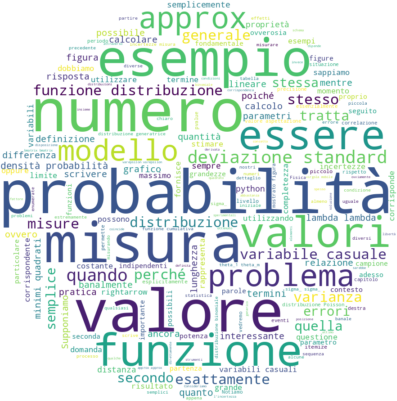
\includegraphics{figures/cover_word_cloud.png}
      \vspace{4\baselineskip}

      % Authors.
      \coauthor{Luca Baldini}{luca.baldini@pi.infn.it}
      \bigskip
      \coauthor{Niccol\`o Di Lalla}{niccolo.dilalla@pi.infn.it}
      \smallskip
      \coauthor{Massimiliano Razzano}{massimiliano.razzano@unipi.it}
      \smallskip
      \coauthor{Carmelo Sgr\`o}{carmelo.sgro@pi.infn.it}
      \vspace{0.1\textheight}

      % Document version.
      \versiontag{6.2.0
}{\today}

      \smallskip

      web: \url{https://github.com/unipi-physics-labs/lab1-notes}

      \smallskip

      \gitrevision{\input{.git/refs/heads/main}}

      \vspace{\baselineskip}
    \end{minipage}
  %}
  \cleardoublepage
  \endgroup}



\begin{document}

\frontmatter

\stattitle


\thispagestyle{empty}

\vspace*{0.4\textheight}

\begin{center}
  
\includegraphics{cc-by-sa}
\end{center}

\bigskip\noindent
This work is licensed under the Creative Commons Attribution-ShareAlike 4.0
International License. To view a copy of this license, visit
\url{http://creativecommons.org/licenses/by-sa/4.0/} or send a letter to
Creative Commons, PO Box 1866, Mountain View, CA 94042, USA.

\cleardoublepage


\dominitoc
\tableofcontents

\chapter*{Prefazione}

Queste dispense sono state compilate a supporto del corso di Laboratorio 1
per gli studenti del primo anno del corso di Laurea in Fisica presso
l'Università di Pisa durante l'anno accademico 2016--2017, e sono state modificate
ed integrate progressivamente negli anni successivi.
Anche se l'impostazione è in parte mutuata dalle dispense della Professoressa
Liana Martinelli (che per anni sono state utilizzate come testo di riferimento
per il corso, e sono adesso liberamente disponibili alla pagina web
\url{https://bitbucket.org/lbaldini/martinelli}) credo si possa dire
senza tema di smentita che i due manoscritti siano abbastanza diversi tra loro
da poterli considerare, a tutti gli effetti, indipendenti.

Il tema centrale delle dispense è quello della rappresentazione e dell'analisi
dei dati. Accanto agli argomenti \emph{classici} che si trovano virtualmente in
qualsiasi testo di carattere introduttivo (elementi di teoria delle probabilità
e di statistica, propagazione degli errori, metodi di \fit) si è cercato di dare
spazio ad elementi appena più avanzati ma indispensabili nel bagaglio di
conoscenze del Fisico (e.g., i metodi Monte Carlo), nella speranza che possano
suscitare interesse e rendere meno arido il materiale.

Il livello della trattazione è il più elementare possibile---compatibilmente
con la sofisticatezza di alcuni concetti che è pur necessario assimilare
in un corso di laboratorio del primo anno. Si dà per scontato che lo studente
sia familiare con il calcolo differenziale ed integrale, principalmente
per funzioni di una variabile, ma, a parte questo, le dispense hanno
l'obiettivo di essere per quanto possibile auto-contenute ed i concetti
necessari sono via via richiamati al momento opportuno.

I punti qualificanti di queste dispense, che derivano direttamente
dall'esperienza di insegnamento accumulata con gli studenti del primo anno,
sono tre:
\begin{itemize}
\item i calcoli sono svolti dall'inizio alla fine, cercando di non saltare
  nessun passaggio intermedio, ed ampiamente commentati---a costo di
  sacrificare a tratti la sintesi e la scorrevolezza del testo;
\item i concetti rilevanti sono illustrati da un gran numero di esempi
  concreti, sviluppati in modo dettagliato, a diversi livelli di
  difficoltà;
\item il testo è corredato da frammenti di codice (in \python) che illustrano
  come si possano implementare in pratica alcuni dei concetti descritti
  in astratto.
\end{itemize}

I frammenti di codice sono particolarmente importanti, perché il laboratorio
è materia che si impara sul campo---ed una comprensione solida della teoria
è utile solo nel limite in cui si riesce a tradurla ed applicarla in pratica.
Gli esempi di codice non sono pensati per essere particolarmente efficienti
o eleganti, ma sono, per la maggior parte, direttamente utilizzabili.
Lo studente ha accesso alla versione elettronica su web di ciascun frammento
di codice attraverso un \foreign{hyperlink} situato nella parte superiore della
cornice corrispondente, e l'\foreign{output} fornito dall'esecuzione è riportato
nella sua interezza in calce al frammento stesso, di modo che sia chiara
non solo l'intenzione, ma anche il risultato.

\begin{snippet}[htb!]
  \bigskip % This is ugly and should be taken care of automagically.
  \hstack[0.45]{\begin{Verbatim}[label=\makebox{\href{https://bitbucket.org/lbaldini/statnotes/src/master/snippets/hello\_world.py}{https://bitbucket.org/.../hello\_world.py}},commandchars=\\\{\}]
\PY{n+nb}{print}\PY{p}{(}\PY{l+s+s1}{\PYZsq{}}\PY{l+s+s1}{Hello world!}\PY{l+s+s1}{\PYZsq{}}\PY{p}{)}

[Output]
Hello world!
\end{Verbatim}}{
    \caption{Illustrazione del più semplice programma realizzabile in \python.
      Si notino l'\foreign{hyperlink} alla versione elettronica nella parte
      superiore della cornice e l'\foreign{output} completo dell'esecuzione
      nella parte inferiore.
    }
    \label{snip:hello_world}
  }
\end{snippet}

Nel corso degli anni il numero e l'importanza dei frammenti di codice nell'economia
delle dispense sono cresciuti progressivamente, fino ad arrivare ad un livello
di integrazione sostanziale tra testo e codice. I linguaggi di programmazione
sono notoriamente argomento che evolve in fretta, e non è banale assicurarsi che
quello che si scrive oggi rimanga rilevante nel tempo. Purtuttavia, l'ecosistema
scientifico di \python\ (\numpy, \scipy, e \matplotlib) è, in questo momento,
ampiamente utilizzato per il calcolo scientifico, da una comunità vasta e vibrante,
per cui speriamo che il materiale possa essere utile non solo didatticamente,
ma anche professionalmente.

\danger%
Di tanto in tanto troverete sezioni che differiscono dalla maggior parte del
resto del contenuto delle dispense---perché focalizzate su argomenti
specifici più avanzati o per il livello leggermente più sofisticato degli
strumenti matematici necessari. Queste sezioni sono indicate con il simbolo
di curva pericolosa e, in una prima lettura, possono essere ignorate senza
che questo pregiudichi la comprensione del resto. (Ma non fatelo
sistematicamente, perché gli argomenti sono interessanti.)

\bigskip

\noindent Che dire di più? Buona lettura!

\bigskip

{\flushright Luca Baldini\\ \flushright Pisa, 21 settembre 2021\\}

\chapter*{Ringraziamenti}

Queste dispense, ve ne accorgerete, sono ancora un lavoro in corso.
Per facilitare la segnalazioni di omissioni ed inesattezze e la raccolta di
suggerimenti abbiamo una pagina web dedicata
\begin{center}
  \url{https://bitbucket.org/lbaldini/statnotes/issues}
\end{center}
in cui chiunque, anche in forma anonima, può contribuire a migliorare il
manoscritto.

Quella che segue è una lista, potenzialmente incompleta, di tutte le persone
(principalmente studenti del corso) che, nel tempo, hanno fornito consigli e
suggerimenti, o più semplicemente hanno fatto domande che hanno generato
cambiamenti nel testo---si spera per il meglio:
Tiziano Andrea Amato,
Anonymous,
Davide Baiocco,
Alessandro Bartalena,
Elia Bianucci,
Edoardo Bogina,
Benedetta Bruno,
Andrea Canzio,
Davide Carducci,
Eva Castagna,
Matteo Chiappini,
Fabrizio Chicconi,
Alberto Cilli,
Alessandro Civolani,
Bruno Danti,
Gaia Da Prato,
Mario Di Luca,
Roberto Dionisio,
Davide Di Virgilio,
Francesco Forti,
Lucrezia Galieni,
Francesco Geroni,
Tommaso Giovannelli,
Filippo Girardi,
William Iania,
Kosimos,
Andrei Lipovanu,
Mattia Martucci,
Giovanni Megliola,
Antonio A.~Mele,
Francesco Mincioni,
Jacopo Omodei,
Luca Palumbo,
Marco Parrinello,
Francesco Pellegrini,
Davide Perrone,
Niccolò Picchiarelli,
Mariella Rinaldi,
Elisa Sabadini,
Gianluca Scardaci,
Nicola Sensi,
Giovanni Spanu,
Alessandro Tauro,
Niccolò Tiezzi,
Bernardo Tomelleri (lo ringrazio due volte, perché l'attenzione con cui ha
letto le dispense è niente meno che impressionante),
Bianca Turini,
Maria Paola Vaccaro,
Matteo Vilucchio.

\bigskip

(Se vi riconoscete in un alias, o banalmente siete stati dimenticati, e volete
che appaia il vostro nome completo non esitate a mandare un messaggio a
\href{mailto:luca.baldini@pi.infn.it}{luca.baldini@pi.infn.it}.)


\mainmatter


%
\chapter{Introduzione}

L'introduzione andrà qui.

%Questo è un esempio di codice.
%\texcode{hello_world}

\chapter{Primi passi: misure ed incertezze}
\label{sec:primi_passi}

Il concetto di \emph{incertezza} o \emph{errore} di misura gioca un ruolo centrale
nelle scienze sperimentali. Visto che non è possibile misurare una grandezza fisica
con accuratezza infinita, il risultato di una misura manca di una parte importante
del proprio contenuto quantitativo in assenza di una stima (implicita o esplicita)
dell'incertezza ad essa associata; quest'ultima è elemento imprescindibile per
poter confrontare una misura con una predizione teorica o con un'altra misura.

Nel linguaggio comune è piuttosto inusuale fare menzione esplicita delle
incertezze di misura: vi immaginate comperare mezzo kilogrammo di pane al
supermercato e chiedere all'inserviente
"potrebbe tagliarlo con una tolleranza di 10 grammi, per cortesia?".
Eppure il fatto che, a fronte di una richiesta di mezzo kilogrammo, 600~grammi
sarebbero probabilmente accettabili dalla maggior parte dei clienti, mentre
2~kilogrammi no, ci dice che in fondo la nozione di errore di misura deve
essere in qualche modo connaturata con il nostro senso comune.

In Fisica, e nelle scienze sperimentali in genere, si cerca tipicamente di
evitare ambiguità ed usare le parole in un modo per quanto possibile
quantitativo e ben definito. Ciò nonostante anche in letteratura scientifica
si trovano occasionalmente diciture in cui l'errore di misura è omesso---di
solito volontariamente e consapevolmente. Anche in questo caso, come vedremo,
è il bagaglio di conoscenze comuni (che cominceremo a sviluppare in questo
capitolo) a guidarci.

In questo primo capitolo introdurremo in parallelo due nozioni di incertezza:
quella \emph{massima} e quella \emph{statistica}---la prima perché non
richiede nessuna nozione pregressa ed è utile per introdurre alcuni concetti
fondamentali, e la seconda perché è quella \emph{corretta} e che
utilizzeremo sin dall'inizio (anche se la giustificheremo rigorosamente solo
nel capitolo~\ref{sec:teoria_dei_campioni}). Ove possibile utilizzeremo la prima
per giustificare intuitivamente, per analogia, alcune \emph{ricette} che daremo
inizialmente senza dimostrazione a proposito della seconda.


\section{Unità di misura e ordini di grandezza}
\label{sec:unita_di_misura}

L'accuratezza delle misure raggiunta in alcune aree della Fisica è niente di
meno che stupefacente. In elettrodinamica quantistica, una delle teorie fisiche
meglio verificate sperimentalmente, il momento magnetico dell'elettrone è
misurato a meglio di una parte su $10^{12}$~\cite{PhysRevA.83.052122}---e la
misura è in accordo con i calcoli teorici, che hanno a loro volta raggiunto un
livello di sofisticazione tale da consentire di avere incertezze dello stesso
ordine di grandezza~\cite{PhysRevLett.109.111807}. Tanto per fissare le idee:
sarebbe come misurare la distanza tra Londra e New York con una precisione di
$1~\mu$m (un millesimo di mm): non sfuggirà la portata dei problemi operativi
connessi con il raggiungimento di un tale livello di riproducibilità, che
costituiscono una delle aree di studio delle moderna metrologia.


\subsection{Il Sistema Internazionale di unità di misura}

Il primo sforzo sistematico dell'età moderna in direzione di un sistema
standard di unità di misura è costituito dalla definizione, nella Francia
della fine del XVIII secolo, del sistema metrico decimale---basato sulle
unità standard di \emph{metro} e \emph{kilogrammo}. Definiti inizialmente
come la decimilionesima parte della lunghezza del meridiano terrestre%
\footnote{La cosa ci porterebbe troppo lontano, ma il lettore curioso è
  incoraggiato a leggere la referenza~\cite{dagostini_metro} per una
  discussione interessante e non convenzionale sull'origine storica della
  definizione del metro.}
e come la massa di $1000$~cm$^3$ di acqua alla temperatura di fusione del
ghiaccio, il metro ed il kilogrammo sono stati ridefiniti circa un secolo più
tardi sulla base di due manufatti (il metro campione ed il kilogrammo campione)
realizzati in una lega di platino-iridio e conservati a Parigi, con un certo
numero di repliche \emph{identiche} distribuite ai principali istituti di
metrologia. \`E chiaro che l'utilizzo di manufatti fisici come unità
fondamentali costituisce di per sé un limite alla riproducibilità delle
misure fisiche. Tanto per fare un esempio, il kilogrammo campione, conservato
insieme a sei copie di riferimento presso il \foreign{Bureau International des Poids et Mesures},
è soggetto ad una contaminazione superficiale al livello di $\sim 1~\mu$g
all'anno. Questa contaminazione, largamente reversibile, rende periodicamente
necessarie sofisticate operazioni di pulizia. Nonostante tutti gli accorgimenti
del caso, tra 1889 al 1989 si è osservata una variazione relativa di massa del
kilogrammo campione rispetto alle sei copie al livello di alcune decine di
$\mu$g~\cite{si_unit_mass}.

Ormai adottato quasi universalmente (sia pure con importanti eccezioni), il
Sistema Internazionale (SI) di unità di misura costituisce ad oggi lo stato
dell'arte nella materia. Il SI include 7 unità di base~\cite{si_brochure}
per la misura di altrettante grandezze fisiche: lunghezza, massa, tempo,
corrente elettrica, temperatura termodinamica, quantità di sostanza ed intensità
luminosa---come mostrato nella tabella~\ref{tab:unita_si}.

\begin{table}[!htb]
  \tablehstack{
    \begin{tabular}{llll}
      \hline
      Quantità & Simbolo & Unità & Simbolo\\
      \hline
      \hline
      Lunghezza & $l$ & metro & m\\
      Massa & $m$ & kilogrammo & kg\\
      Tempo & $t$ & secondo & s\\
      Corrente elettrica & $I$, $i$ & ampere & A\\
      Temperatura & $T$ & kelvin & K\\
      Quantità di sostanza & $n$ & mole & mol \\
      Intensità luminosa & $I_\nu$ & candela & cd\\
      \hline
    \end{tabular}
  }{
    \caption{Tabella delle 7 grandezze fisiche di base, con relative unità di
      misura, su cui è fondato il Sistema Internazionale.
      (Adattato da~\cite{si_brochure}.)}
    \label{tab:unita_si}
  }
\end{table}

Storicamente, le unità fondamentali sono state definite in vario modo---utilizzando
manufatti come il metro ed il kilogrammo campione, stati specifici della
materia come il punto triplo dell'acqua, costanti fondamentali della natura come
la velocità della luce, o prescrizioni sperimentali idealizzate.
A partire dal 20 maggio 2019, \emph{il Sistema Internazionale è definito sulla
base del valore numerico di 7 costanti fondamentali della Natura, che si
assumono note esattamente}. In particolare, il SI è il sistema in cui:
\begin{itemize}
\item la frequenza della transizione iper-fine dello stato fondamentale non
  perturbato dell'atomo di $^{133}$Cs vale esattamente
  $\Delta\nu_{Cs} = 9\,192\,631\,770$~Hz;
\item la velocità della luce nel vuoto vale esattamente $c = 299\,792\,458$~m~s$^{-1}$;
\item la costante di Planck vale esattamente $h = 6.626\,070\,15 \times 10^{-34}$~J~s;
\item la carica elementare vale esattamente $e = 1.602\,176\,634 \times 10^{-19}$~C;
\item la costante di Boltzmann vale esattamente $k = 1.380\,649 \times 10^{-23}$~J~K$^{-1}$;
\item il numero di Avogadro vale esattamente $N_A = 6.022\,140\,76 \times 10^{23}$~mol$^{-1}$;
\item l'efficacia luminosa della radiazione monocromatica di frequenza
  $540 \times 10^{12}$~Hz vale esattamente $K_{cd} = 683$~lm~W$^{-1}$.
\end{itemize}
Così, ad esempio, il secondo corrisponde alla durata di $9\,192\,631\,770$
periodi della transizione tra i due livelli iper-fini dello stato fondamentale
dell'atomo di $^{133}$Cs, ed il metro è la lunghezza percorsa dalla luce nel
vuoto in un intervallo di tempo pari a $1/299\,792\,458$~s.

Arrivare ad un sistema in cui tutte le unità fondamentali sono definite in
termini di \emph{invarianti} della natura, affrancandosi dalla necessità di
ricorrere a manufatti, costituisce un traguardo fondamentale per la metrologia
moderna, che ha richiesto uno sforzo lungo più di un secolo.
Ed il Sistema Internazionale è in continua evoluzione, nel tentativo di rispondere
alle esigenze sempre più stringenti dalla scienza e della tecnologia moderna.


\subsection{Unità derivate ed unità riconosciute}

Alcune unità di misura derivate hanno, nel Sistema Internazionale, nomi speciali,
che corrispondono ad una forma convenientemente compatta di combinazioni specifiche
delle 7 unità di base. Una lista parziale di queste unità derivate è presentata nella
tabella~\ref{tab:unita_derivate_si}. (Notate che, ove l'unità di misura prenda il
nome da una persona---tipicamente un illustre scienziato---si scrive convenzionalmente
con la prima lettera minuscola.)

\begin{table}[!htb]
  \tablehstack{
    \begin{tabular}{llll}
      \hline
      Quantità & Unità & Simbolo & Espressione SI\\
      \hline
      \hline
      Angolo & radiante & rad & -\\
      Angolo solido & steradiante & sr & -\\
      Frequenza & hertz & Hz & s$^{-1}$ \\
      Forza & newton & N & m~kg~s$^{-2}$ \\
      Pressione & pascal & Pa & m$^{-1}$~kg~s$^{-2}$ \\
      Energia & joule & J & m$^2$~kg~s$^{-2}$ \\
      Potenza & watt & W & m$^2$~kg~s$^{-3}$ \\
      Temperatura Celsius & grado Celsius & $^\circ$C & K\\
      Carica elettrica & coulomb & C & s~A \\
      Potenziale elettrico & volt & V & m$^2$~kg~s$^{-3}$~A$^{-1}$\\
      Capacità & farad & F & m$^{-2}$~kg$^{-1}$~s$^{4}$~A$^{2}$ \\
      Resistenza & ohm & $\Omega$ & m$^{2}$~kg~s$^{-3}$~A$^{-2}$ \\
      Attività & becquerel & Bq & s$^{-1}$\\
      \hline
    \end{tabular}
  }{
    \caption{Lista (non esaustiva) delle unità derivate che hanno nomi
      speciali nel Sistema Internazionale. Le corrispondenti espressioni in
      termini delle 7 unità fondamentali del Sistema Internazionale sono
      mostrate esplicitamente nell'ultima colonna.
      (Adattato da~\cite{si_brochure}.)
      \label{tab:unita_derivate_si}}
  }
\end{table}

In generale l'espressione, in termini delle unità fondamentali del SI, per una
generica grandezza derivata si ricava, più o meno banalmente, da una
qualsiasi legge fisica che coinvolga l'unità derivata. Così, dalla legge di
Newton
\begin{align*}
  F = ma \quad \text{[m~kg~s$^{-2}$]}
\end{align*}
sappiamo che la forza è una massa (kg) per un'accelerazione (m~s$^{-2}$),
per cui il newton corrisponde a m~kg~s$^{-2}$; una pressione, d'altra parte,
è una forza per unità di superficie (m$^2$)
\begin{align*}
  p = \frac{F}{A} \quad \text{[m$^{-1}$~kg~s$^{-2}$]}
\end{align*}
per cui il pascal corrisponde a m$^{-1}$~kg~s$^{-2}$; l'energia (o il lavoro) è
il prodotto di una forza per uno spostamento (m),
\begin{align*}
L = F s \quad \text{[m$^2$~kg~s$^{-2}$]}
\end{align*}
per cui si misura in m$^2$~kg~s$^{-2}$, e così via.

Vi è infine un certo numero di unità di misura che, pur non facendo parte
del Sistema Internazionale, sono così comunemente usate (ad esempio il
litro per le misure di volume) o sono così profondamente radicate nella
nostra cultura (ad esempio le ore, i minuti ed i secondi per le misure di tempo)
da essere ufficialmente riconosciute ed accettate, come illustrato nella
tabella~\ref{tab:unita_non_si}.
(Per inciso: l'atmosfera, che corrisponde a $101325$~Pa, non fa parte delle
unità riconosciute.)

\begin{table}[!htb]
  \tablehstack{
    \begin{tabular}{llll}
      \hline
      Quantità & Unità & Simbolo & Conversione SI\\
      \hline
      \hline
      Tempo & minuto & min & $1~\text{min} = 60~\text{s}$\\
      & ora & h & $1~\text{h} = 3600~\text{s}$\\
      & giorno & d & $1~\text{d} = 86\,400~\text{s}$\\
      Volume & litro & l & $1~\text{l} = 1~\text{dm}^3$\\
      Massa & tonnellata & t & $1~\text{t} = 1000~\text{kg}$\\
      Energia & electronvolt & eV &
      $1~\text{eV} \approx 1.602 \times 10^{-19} ~\text{J}$ \\
      & erg & erg & $1~\text{erg} = 10^{-7}~\text{J}$ \\
      Pressione & bar & bar & $1~\text{bar} = 10^5~\text{Pa}$ \\
      & mm di Hg & mmHg & $1~\text{mmHg} \approx 133.3~\text{Pa}$ \\
      \hline
    \end{tabular}
  }{
    \caption{Lista (non esaustiva) delle unità che, pur non facendo parte
      del Sistema Internazionale, sono riconosciute in quanto culturalmente o
      storicamente rilevanti. (Adattato da~\cite{si_brochure}.)
      \label{tab:unita_non_si}}
  }
\end{table}


\subsection{Multipli, sottomultipli ed ordini di grandezza}

Le grandezze oggetto di studio in Fisica possono differire tra loro di
numerosi ordini di grandezza. Così, mentre il raggio di un protone è
dell'ordine di $10^{-15}$~m, le sorgenti astronomiche più lontane si
trovano a distanze di svariati Gpc (gigaparsec), cioè a distanze dell'ordine
di~$10^{26}$~m.
Analogamente, mentre la vita media dei bosoni $W$ e $Z_0$ è dell'ordine di
$10^{-25}$~s, l'età del nostro universo è dell'ordine di 10~miliardi di
anni, o $10^{17}$~s. In entrambi i casi la \emph{gamma dinamica} corrisponde a
più di $40$ ordini di grandezza.
A questo scopo il Sistema Internazionale definisce una serie di prefissi
per facilitare la scrittura di grandezze il cui valore sia molto più piccolo
o molto più grande della relativa unità di misura, come mostrato in
tabella~\ref{tab:prefissi_si}.

\begin{table}[!htb]
  \tablehstack{
    \begin{tabular}{llllll}
      \hline
      Fattore & Nome & Simbolo & Fattore & Nome & Simbolo\\
      \hline
      \hline
      $10^{1}$  & deca  & da & $10^{-1}$ & deci & d\\
      $10^{2}$  & hecto & h  & $10^{-2}$ & centi & c\\
      $10^{3}$  & kilo  & k  & $10^{-3}$ & milli & m\\
      $10^{6}$  & mega  & M  & $10^{-6}$ & micro & $\mu$\\
      $10^{9}$  & giga  & G  & $10^{-9}$ & nano & n\\
      $10^{12}$ & tera  & T  & $10^{-12}$ & pico & p\\
      $10^{15}$ & peta  & P  & $10^{-15}$ & femto & f\\
      $10^{18}$ & exa   & E  & $10^{-18}$ & atto & a\\
      $10^{21}$ & zetta & Z  & $10^{-21}$ & zepto & z\\
      $10^{24}$ & yotta & Y  & $10^{-24}$ & yocto & y\\
      \hline
    \end{tabular}
  }{
    \caption{Prefissi per i multipli e sottomultipli decimali delle unità di
      misura del Sistema Internazionale. Il kg si trova nella situazione
      peculiare di rappresentare una delle unità fondamentali pur essendo
      preceduto dal prefisso k. (Adattato da~\cite{si_brochure}.)
      \label{tab:prefissi_si}}
  }
\end{table}

\section{Cenni di analisi dimensionale}
\label{sec:calcolo_dimensionale}

Quando si ha a che fare con un sistema fisico descritto da grandezze non
adimensionali, le equazioni che lo descrivono debbono soddisfare il requisito
di base di essere \emph{dimensionalmente corrette}---cioè le dimensioni
fisiche dei due membri devono essere omogenee. In caso contrario l'equazione
è banalmente sbagliata. Controllare sistematicamente le dimensioni fisiche
in ogni passaggio di un calcolo permette spesso di evitare errori banali.

Nel seguito indicheremo le dimensioni fisiche di una generica grandezza
con il simbolo corrispondente in tabella~\ref{tab:unita_si} racchiuso in
parentesi quadre. Così, e.g.,  diremo che il raggio della Terra ha le
dimensioni di una lunghezza, che indicheremo con $[l]$. Le grandezze derivate
seguono le regole del prodotto, e le dimensioni fisiche di una velocità,
e.g., sono quelle di una lunghezza per l'inverso di un tempo, o $[l~t^{-1}]$.

Supponiamo allora di essere interessati alla relazione che lega il periodo
$T$ di un pendolo alla sua lunghezza $l$. Se qualcuno scrivesse
\begin{align*}
  T = 2\pi \frac{l}{g} \quad \text{(dimensionalmente non corretta)}
\end{align*}
potremmo smentire l'affermazione, anche ignorando le leggi fondamentali della
meccanica, sulla base del fatto che le dimensioni fisiche del membro di destra
dell'equazione sono quelle di un tempo al quadrato e non quelle di un tempo
\begin{align*}
  [t] \neq [l] \times [l~t^{-2}]^{-1} = [t^{2}]
\end{align*}

L'analisi dimensionale, se utilizzata opportunamente, può anche avere potere
predittivo. Nel caso specifico, se ipotizziamo che il periodo $T$ possa
dipendere dalla lunghezza $l$ del pendolo e dalla sua massa $m$, oltre che
dall'accelerazione di gravità $g$, ci troviamo con il problema di capire
quali siano le combinazioni funzionali di queste tre grandezze che forniscono
una quantità con le dimensioni fisiche giuste. Se partiamo dall'ipotesi di
lavoro (arbitraria, ma non irragionevole) che il periodo cercato si possa
scrivere nella forma
\begin{align*}
  T = l^{\alpha_1} m^{\alpha_2} g^{\alpha_3},
\end{align*}
allora da un punto di vista dimensionale possiamo scrivere
\begin{align*}
  [t] = [l]^{\alpha_1} \times [m]^{\alpha_2} \times [l~t^{-2}]^{\alpha_3} =
  [l]^{\alpha_1 + \alpha_3} \times [m]^{\alpha_2} \times [t]^{-2\alpha_3},
\end{align*}
che a sua volta può essere trasformato nel sistema di equazioni
\begin{align*}
  \begin{cases}
    \alpha_1 + \alpha_3 = 0\\
    \alpha_2 = 0\\
    -2\alpha_3 = 1
  \end{cases}
  \text{ossia} \quad
  \begin{cases}
    \alpha_1 = 1/2\\
    \alpha_2 = 0\\
    \alpha_3 = -1/2.
  \end{cases}
\end{align*}
In questo caso specifico l'analisi dimensionale da sola ci permette dunque di
concludere che il periodo del pendolo non può dipendere dalla massa (a meno
che non inseriamo nel problema dall'esterno un'ulteriore grandezza che abbia
la massa nelle sue dimensioni fisiche, ad esempio nella forma di un coefficiente
di attrito viscoso) e che l'equazione cercata deve essere nella forma
\begin{align*}
  T \propto \sqrt{\frac{l}{g}}.
\end{align*}
Come sappiamo la conclusione è corretta ed il fattore di proporzionalità
è, nel limite di piccole oscillazioni, $2\pi$. Per completezza, come
vedremo nella sezione~\ref{sec:piccole_oscillazioni}, nel caso di ampiezza
iniziale $\theta_0$ non nulla si ha un ulteriore fattore moltiplicativo
adimensionale, funzione di $\theta_0$ che non si può ovviamente ricavare per
via dimensionale.

In generale, se siamo interessati alla relazione funzionale che lega una
generica grandezza $y$ ad una serie di grandezze $x_1, x_2 \ldots x_n$
possiamo---anche se non vi è garanzia che questo funzioni---provare a
scrivere la grandezza cercata nella forma
\begin{align}
  y = x_1^{\alpha_1}x_2^{\alpha_2} \ldots x_n^{\alpha_n}.
\end{align}
Il requisito che l'equazione scritta sopra sia dimensionalmente corretta può
essere trasformato in un sistema di equazioni lineari per gli esponenti
$\alpha_1, \alpha_2 \ldots \alpha_n$ che a sua volta può fornire informazioni
non banali sul sistema che stiamo studiando, come illustrato
nell'esempio~\ref{exp:calcolo_dimensionale_keplero}.
Per completezza gli argomenti che abbiamo illustrato brevemente in questa
sezione si possono sviluppare in modo rigoroso e costituiscono il contenuto del
celebre teorema~$\pi$~\cite{teorema_pi}.


\begin{examplebox}[htb]
  \begin{example}[terza legge di Keplero]
    \label{exp:calcolo_dimensionale_keplero}
    Ci proponiamo di ricavare per via dimensionale la terza legge di Keplero,
    ossia la relazione che lega il periodo orbitale $T$ di un pianeta al
    semiasse maggiore $a$ della sua orbita. Assumeremo che gli ulteriori
    parametri che entrano nel problema siano la costante di gravitazione
    universale $G$ e la massa del Sole $m_\odot$ e che possiamo scrivere la
    relazione cercata come $T = G^{\alpha_1} m_\odot^{\alpha_2} a^{\alpha_3}$.
    (Se a questo punto vi state chiedendo perché non abbiamo incluso la
    massa del pianeta nella lista\ldots\ si tratta di un'ottima domanda, cui
    l'analisi dimensionale da sola non fornisce una risposta soddisfacente,
    ma procediamo ugualmente e vediamo dove ci porta il nostro ragionamento.)
    Le unità di misura di $G$ si possono ricavare, e.g. dalla legge di
    gravitazione universale
    \begin{align}
      F = G \frac{m_1 m_2}{r^2} \quad \text{da cui} \quad
      G = \frac{Fr^2}{m_1 m_2}
    \end{align}
    e sono, nel sistema internazionale m$^3$~kg$^{-1}$~s$^{-2}$. Ragionando come
    prima si ha allora
    \begin{align*}
      [t] = [l^3~m^{-1}~t^{-2}]^{\alpha_1} \times [m]^{\alpha_2} \times [l]^{\alpha_3} =
      [l]^{3\alpha_1 + \alpha_3} \times [m]^{\alpha_2 - \alpha_1} \times [t]^{-2\alpha1},
    \end{align*}
    da cui
     \begin{align}\label{eq:legge_di_keplero}
      \begin{cases}
        3\alpha_1 + \alpha_3 = 0\\
        \alpha_2 - \alpha_1 = 0\\
        -2\alpha_1 = 1
      \end{cases}
      \quad \text{ossia} \quad
      \begin{cases}
        \alpha_1 = -1/2\\
        \alpha_2 = -1/2\\
        \alpha_3 = 3/2.
      \end{cases}
      \quad \text{e infine} \quad
      T \propto \frac{a^{\frac{3}{2}}}{\sqrt{Gm_\odot}}.
     \end{align}
     La conclusione (tutt'altro che ovvia) è corretta ed il fattore di
     proporzionalità è di nuovo $2\pi$---ma, va da sé, si tratta di una
     semplice coincidenza.
  \end{example}
\end{examplebox}


\section{Il concetto di incertezza di misura}
\label{sec:errore_max}

Nella sua formulazione più elementare, il concetto di \emph{errore massimo}
è legato alla domanda: "qual è il più piccolo intervallo che contiene
con certezza il valore numerico della quantità che sto misurando?"
In altre parole, se scriviamo il risultato della misura di una generica
grandezza fisica $x$ come:
\begin{align}\label{eq:errore_max}
  x = \hat{x} \pm \Delta x~\text{[unità di misura]}
\end{align}
intendendo $\Delta x$ come errore massimo, allora in effetti stiamo dicendo che
l'intervallo $[\hat{x} - \Delta x, \hat{x} + \Delta x]$ è il più piccolo
intervallo possibile che ci dia la certezza di includere il valore (incognito)
di~$x$. Se scriviamo, ad esempio, $l = 12.4 \pm 0.2$~cm, stiamo dicendo di
essere certi che $l$ sia compreso tra $12.2$ e~$12.6$~cm, e che l'intervallo
$[12.2, 12.6]$~cm è il più piccolo che ci possa dare tale certezza.

Gli ingredienti della~\eqref{eq:errore_max} hanno ciascuno un significato ben
preciso che è bene fissare il prima possibile:
\begin{itemize}
\item $x$ è il valore, incognito, della grandezza che vogliamo misurare, che
  chiameremo \emph{misurando} (cercando deliberatamente di evitare l'espressione
  \emph{valore vero}, che pure si trova usata in letteratura);
\item $\hat{x}$ è la \emph{miglior stima} di $x$ che possiamo fornire a
  partire dai dati a nostra disposizione---che chiameremo anche
  \emph{valore centrale} o \emph{migliore stima} della misura;
\item $\Delta x$ è l'incertezza di misura---o più precisamente, in questo
  contesto, l'\emph{errore massimo}, nel senso che abbiamo
  precisato sopra. (Notiamo che, per definizione, $\Delta x$ rappresenta la
  lunghezza di un intervallo ed è perciò una grandezza definita positiva.)
\end{itemize}
Vale la pena sottolineare che il risultato di una misura non ha senso se non
sono indicate, ove necessario, le unità di misura.

Quando il risultato di una misura fluttua, la nozione di errore massimo porta
in sé una contraddizione logica dovuta al fatto che, da un punto di vista
operativo, non è possibile garantire a priori che una nuova misura della
stessa grandezza non fornisca un valore al di fuori dell'intervallo iniziale di
incertezza. Ove questo accada siamo costretti ad allargare tale intervallo---ci
troviamo, cioè, nella situazione assurda in cui acquisire nuova informazione
può solo peggiorare (o, al massimo, lasciare invariato) il nostro stato di
conoscenza, nella misura in cui esso è determinato dall'incertezza di misura.

Questo è il motivo per cui in pratica non useremo \emph{mai} il concetto
di errore massimo, ma utilizzeremo fin da subito quello che comunemente va
sotto il nome di errore statistico:
\begin{align}\label{eq:errore_stat}
  x = \hat{x} \pm \sigma_x~\text{[unità di misura]}.
\end{align}
La~\eqref{eq:errore_stat} ha un significato fondamentalmente diverso
dalla~\eqref{eq:errore_max}: come vedremo in dettaglio nel
capitolo~\ref{sec:teoria_dei_campioni} essa definisce un intervallo che non ci
dà la \emph{certezza}, ma solo una \emph{probabilità} ben definita di
contenere il valore del misurando. (Purtroppo introdurremo il concetto di
probabilità solo nel capitolo~\ref{sec:probabilita}.)
A questo livello potrebbe sembrare una mera questione di notazione (una
$\sigma$ al posto di una $\Delta$), ma si tratta in realtà di una differenza
profonda e carica di conseguenze.


\subsection{Errore assoluto ed errore relativo}
\label{sec:errore_assoluto_relativo}

Definiamo \emph{errore relativo} (detto anche \emph{errore percentuale}) il
rapporto tra l'incertezza della misura (detta anche \emph{errore assoluto}) ed
il suo valore centrale. In particolare, utilizzando la nostra notazione:
\begin{align}\label{eq:errore_max_relativo}
  \text{Errore relativo} := \frac{\sigma_x}{\abs{\hat{x}}}.
\end{align}
Poiché l'incertezza ha, per ovvie ragioni, le stesse dimensioni fisiche della
misura a cui si riferisce, l'errore relativo è una quantità adimensionale
(e definita positiva).

\begin{examplebox}
  \begin{example}
    Si misura una lunghezza $l$ ottenendo il risultato $l = 12.4 \pm 0.2$~cm.
    L'errore relativo è in questo caso $0.016$, vale a dire $1.6\%$.
  \end{example}
\end{examplebox}


\subsection{Precisione ed accuratezza}

In letteratura si trova la distinzione tra i concetti di \emph{accuratezza},
intesa come accordo tra il valore della misura e quello del misurando, e di
\emph{precisione}, intesa come consistenza tra risultati di successive misure
della stessa quantità nelle medesime condizioni.

Si tratta di una distinzione molto rilevante, poiché un dato strumento può
essere molto accurato ma poco preciso (se fornisce in media la risposta giusta,
ma con fluttuazioni rilevanti tra misurazioni successive) o---il che è
potenzialmente più pericoloso---molto preciso ma poco accurato (se fornisce
in modo estremamente riproducibile la risposta sbagliata). Avremo tempo di
tornare sull'argomento in seguito, ma diciamo fin da subito che cercheremo
scrupolosamente di usare questi due termini nell'accezione appena indicata.

\pgffigfour[!b]{precisione_accuratezza_1}{precisione_accuratezza_2}{precisione_accuratezza_3}{precisione_accuratezza_4}{
  Illustrazione grafica dei concetti di precisione ed accuratezza
  (adattato da \url{https://www.roma1.infn.it/~dagos/BMS/node116.html}).
  In tutte e quattro le figure la linea verticale rappresenta il misurando
  mentre la curva serve a dare un'idea, che a
  questo livello è puramente qualitativa, delle fluttuazioni delle misure
  attorno al misurando stesso. Va da sé che gli aggettivi "buono" e
  "scarso" debbono essere intesi in senso relativo, come metrica di
  confronto tra le varie situazioni.
}

Per completezza, la figura~\ref{fig:precisione_accuratezza_1_four} illustra
graficamente i concetti di precisione ed accuratezza che abbiamo appena
definito. In ciascuno dei quattro grafici la curva rappresenta in modo
qualitativo le fluttuazioni delle misure attorno al misurando (incognito), che
è a sua volta indicato dalla linea verticale. Con leggero abuso di
linguaggio potremmo dire che la precisione ha a che vedere con la larghezza
della curva, mentre l'accuratezza ha a che vedere con la vicinanza tra il
massimo della curva ed il misurando.


\section{Cifre significative e convenzioni di scrittura}
\label{sec:cifre_significative}

Prima ancora di capire come si stima in pratica l'incertezza massima di misura,
ci soffermiamo per un attimo su alcune questioni, semplici ma importanti, di
notazione. In un articolo scientifico non troverete mai scritto (sperabilmente)
che la massa di un oggetto è $74.562572 \pm 0.024894$~kg. Ed il motivo è
semplice: se l'errore di misura è dell'ordine di 25~g, è palesemente
assurdo scrivere il valore centrale fino al~$\mu$g (cioè fino al millesimo di
mg!). Le ultime tre cifre (almeno) sono irrilevanti---semplice rumore numerico.

Facciamo un passo indietro. La questione si può inquadrare quantitativamente
attraverso la nozione di \emph{cifra significativa}, che si definisce mediante
tre semplici regole, illustrate dall'esempio~\ref{exp:cifre_significative}.
Dato un valore generico:
\begin{itemize}
\item la cifra più significativa è quella più a sinistra diversa
  da zero;
\item la cifra meno significativa è quella più a destra (inclusi gli
  zeri a destra del separatore decimale, ma fatta eccezione per gli zeri che
  definiscono l'ordine di grandezza per i numeri interi);
\item tutte le cifre comprese tra la più significativa e la
  meno significativa sono significative.
\end{itemize}

\begin{examplebox}
  \hstack[0.8]{\begin{example}\label{exp:cifre_significative}
      Negli esempi qui di fianco indichiamo con una sottolineatura la cifra meno
      significativa, con una sopralineatura quella più significativa e tra
      parentesi quadre il numero di cifre significative, in una serie di
      situazioni tipiche. (Si tratta di una cosa di importanza basilare, per cui
      assicuratevi di dominare l'argomento prima di procedere.)
  \end{example}}{
    \vspace*{7pt}
    \rule{12pt}{0pt}%
    \begin{tabular}{ll}
      $\overline{3}11\underline{5}$ & [$4$]\\
      $\overline{3}212.\underline{5}$ & [$5$]\\
      $0.0\overline{3}2\underline{5}$ & [$3$]\\
      $0.0\overline{3}0\underline{0}$ & [$3$]\\
      $\overline{3}00.0\underline{0}$ & [$5$]
    \end{tabular}
  }
\end{examplebox}

Torniamo allora al nostro problema originale. La nozione di cifra significativa
è strettamente connessa con quella di arrotondamento del valore centrale
della misura ed il numero di cifre significative con cui si deve scrivere tale
valore è determinato dall'incertezza associata. Più precisamente:
\emph{si scrive l'incertezza di misura con una o al massimo due cifre
  significative (arrotondando opportunamente), e si arrotonda il valore
  centrale in modo da essere consistente, in termini di cifre decimali, con
  l'incertezza associata}.

Così $74.563 \pm 0.025$~kg e $74.56 \pm 0.02$~kg sono entrambe scritture
accettabili per la massa dell'oggetto con cui abbiamo aperto questa sezione.
(Va da sé che, quando i risultati di misure, dirette o indirette, vengono
usati per stimare grandezze derivate, è buona norma avere cura che gli
arrotondamenti effettuati nei passaggi intermedi non introducano errori
significativi nel risultato finale.) Il lettore è incoraggiato ad esaminare
scrupolosamente l'esempio~\ref{exp:errori_cifre_significative}, che rappresenta
un breve campionario di modi in cui \emph{non} scrivere il risultato della
misura.

\begin{examplebox}
  \begin{example}\label{exp:errori_cifre_significative}
    La seguente è una breve lista di errori tipici che si possono compiere;
    i valori tra parentesi quadre indicano la (o una) possibile versione
    corretta.

    \medskip
    \begin{tabular}{l@{\hskip 18pt}l@{\hskip 18pt}l}
      $3.436 \pm 0.542$ & incertezza con troppe (tre) cifre significative &
      [$3.44\pm0.54$]\\
      $3.4 \pm 0.54$ & incertezza con una cifra significativa di troppo &
      [$3.4 \pm 0.5$]\\
      & oppure valore centrale con una cifra significativa mancante &
      [$3.40 \pm 0.54$]\\
      $3.44 \pm 0.5$ & valore centrale con una cifra significativa di troppo &
      [$3.4 \pm 0.5$]\\
      & oppure incertezza con una cifra significativa mancante &
      [$3.44 \pm 0.50$]\\
      $3000 \pm 100$ & scrittura ambigua per gli zeri meno significativi &
      [$(3.0 \pm 0.1)\times 10^3$]
    \end{tabular}
  \end{example}
\end{examplebox}

La capacità di scrivere correttamente il risultato di una misura è di
fondamentale importanza e va acquisita il prima possibile. Troncare l'incertezza
di misura a una o due cifre significative può a prima vista apparire come una
genuina perdita di informazione, ma è importante realizzare subito che così
non è, perché le cifre che tronchiamo
\emph{non contengono nessuna informazione}.
Se misuriamo la lunghezza di un tavolo con un metro a nastro non c'è nessuna
informazione utile nella cifra corrispondente ad $1~\mu$m; quando ci pesiamo su
una bilancia pesapersone non c'è nessuna informazione utile nella cifra
corrispondente al decimo di grammo. Per cui, lo ripetiamo perché non vi
è rischio di enfatizzare troppo il concetto,
\emph{scrivere un'incertezza con più di due cifre significative non ha alcun
  senso}. Nella maggior parte dei casi una è sufficiente.

Per completezza notiamo che non è inconsueto in letteratura che l'incertezza
di misura venga (consapevolmente) omessa. In questi casi la precisione del
risultato sperimentale è, almeno parzialmente, implicita nel modo in cui il
risultato stesso è scritto, e si può assumere che l'errore sia da
considerarsi pari ad una unità della cifra meno significativa del valore
centrale. Così i valori $5.0$~m, e $5.00$~m hanno significati diversi:
il primo è da leggersi come $5.0 \pm 0.1$~m, mentre il secondo come
$5.00 \pm 0.01$~m. Inutile a dirsi, riportare esplicitamente l'errore di misura
è il modo migliore per evitare ambiguità di sorta.


\subsection{Alcune precisazioni sugli arrotondamenti}

Nella sezione precedente abbiamo accennato sommariamente al problema degli
arrotondamenti, ma ci sono un paio di dettagli che vale la pena sviscerare
prima di procedere.

Tecnicamente per \emph{arrotondamento} si intende il processo di riduzione
del numero di cifre significative con cui si rappresenta una quantità fisica.
L'arrotondamento può essere per difetto, se il valore arrotondato è minore
di quello originale, e per eccesso in caso contrario. Ove non si specifichi
altrimenti, si dà per inteso che gli arrotondamenti si eseguono in modo
che il valore arrotondato sia quello più vicino a quello originale. Così, se
vogliamo arrotondare a 2~cifre significative si ha
\begin{align*}
  3.21 & \rightarrow 3.2 \quad \text{(arrotondamento per difetto)} \\
  3.27 & \rightarrow 3.3 \quad \text{(arrotondamento per eccesso).}
\end{align*}

Tecnicamente questa prescrizione non è ben definita quando i valori
arrotondati per eccesso e per difetto sono equidistanti dal valore originale,
e.g.,
\begin{align*}
  3.25 \rightarrow\ ? \quad \text{(arrotondamento per difetto o per eccesso?).}
\end{align*}
In questi casi arrotondare sempre per difetto o sempre per eccesso porterebbe
ad una sottostima o una sovrastima sistematica (e potenzialmente pericolosa)
delle misure---che è per ovvie ragioni da evitare. Una prescrizione possibile
è allora arrotondare per difetto se la cifra a sinistra del $5$ è pari
(come è il $2$ in questo caso) ed arrotondare per eccesso se la cifra è
dispari%
\footnote{Tecnicamente l'idea funziona se la frequenza delle cifre pari è
  uguale a quella delle cifre dispari---cosa che, pur essendo apparentemente
  ragionevole, a rigore non è garantita, come vedremo nella
  sezione~\ref{sec:legge_di_benford}.
  Ma abbiamo discusso il problema a sufficienza ed è arrivato il momento di
  dichiararci soddisfatti e procedere.}%
:
\begin{align*}
  3.25 & \rightarrow 3.2 \quad \text{(arrotondamento per difetto)} \\
  3.35 & \rightarrow 3.4 \quad \text{(arrotondamento per eccesso).}
\end{align*}


\section{Digressione: \python\ come calcolatore tascabile}

Interrompiamo per un attimo il filo della discussione per introdurre \python,
il linguaggio di programmazione che ci accompagnerà lungo tutto il nostro
viaggio. Per poter essere utilizzati, gli esempi inclusi in questa sezione, e
quelli che seguiranno, presuppongono che abbiate un'installazione funzionante
di \python. Sottolineiamo che queste dispense non hanno la benché minima pretesa
di essere un corso auto-contenuto di \python, ed il lettore che non fosse già
familiare con la materia avrà bisogno senza dubbio di risorse aggiuntive per
mettersi in condizione di utilizzare gli esempi mostrati nel seguito---ma il
\foreign{web} è letteralmente stracolmo di istruzioni e \emph{tutorial} al
proposito, per cui non dovrebbe essere difficile trovare quello che fa più al
caso vostro.

Nella modalità di utilizzo più semplice, \python\ può essere usato in modo
\emph{interattivo}---ovvero lanciando l'interprete da linea di comando ed
inserendo comandi \python\ (validi) nell'interprete stesso. La cosa è
interessante perché in questa modalità l'interprete \emph{risponde} ad
ogni comando stampando sullo schermo il risultato del comando stesso ogni qual
volta si preme il tasto di invio, cosa che può risultare utile di tanto in
tanto---specialmente quando si sperimenta.

L'esempio che segue illustra l'utilizzo di \python\ come una sorta di calcolatore
tascabile. Notiamo in particolare:
\begin{itemize}
\item le quattro operazioni elementari sono implementate attraverso gli
  operatori \cchar{+}, \cchar{-}, \cchar{*} e \cchar{/}, con le consuete regole
  di precedenza;
\item l'operatore \cchar{**} (che ha precedenza sui quattro elencati sopra)
  corrisponde all'elevamento a potenza;
\item la funzione \code{round()} permette di arrotondare un numero reale
  all'intero più vicino.
\end{itemize}

\begin{Verbatim}
[lbaldini@nbbaldini ~]$ python
Python 3.7.4 (default, Jul  9 2019, 16:32:37)
[GCC 9.1.1 20190503 (Red Hat 9.1.1-1)] on linux
Type "help", "copyright", "credits" or "license" for more information.
>>> (3 + 3) / 2.2
2.727272727272727
>>> 2.4 * 15.3
36.72
>>> 3.**2.
9.0
>>> round(2.49)
2
>>> round(2.51)
3
>>>
\end{Verbatim}

Chi non avesse già familiarità con la cosa è vivamente incoraggiato ad
aprire un interprete \python\ e sperimentare. Non vi è rischio di rompere
niente ed è un buon modo per prepararsi al lavoro vero che arriverà a breve!

Nella stragrande maggioranza dei casi, tuttavia, non lavoreremo in modalità
interattiva; scriveremo viceversa la nostra serie di comandi in un \emph{file}
di testo nella forma di un \emph{programma} che l'interprete esegue
sequenzialmente. Questo ha il vantaggio che il lavoro che facciamo non va
perduto al termine della sessione interattiva, ma può essere salvato,
modificato, condiviso ed eseguito all'occorrenza. Essere capaci di scrivere ed
eseguire il nostro primo programma, per quanto semplice, è il secondo passo
fondamentale verso l'arte della programmazione. Da qui in poi la strada è in
discesa.

Come vedremo, gli strumenti che l'interprete \python\ mette a disposizione di
\emph{default} all'avvio non ci basteranno. Dovremo utilizzare una serie
di librerie, sia dalla libreria standard di \python\ che da pacchetti esterni,
che implementano funzionalità più avanzate, e che vedremo via via. La
libreria \code{math}, ad esempio, mette a disposizione una serie di costanti
(e.g., $\pi$) e di funzioni matematiche (esponenziale, logaritmi, funzioni
trigonometriche) che ci saranno utili in seguito.

\begin{snippet}[htb!]
  \bigskip % This is ugly and should be taken care of automagically.
  \hstack[0.45]{\begin{Verbatim}[label=\makebox{\href{https://bitbucket.org/lbaldini/statnotes/src/master/snippets/rounding.py}{https://bitbucket.org/.../rounding.py}},commandchars=\\\{\}]
\PY{k+kn}{import} \PY{n+nn}{math}

\PY{n}{a} \PY{o}{=} \PY{l+m+mf}{2.34}
\PY{c+c1}{\PYZsh{} Various roundings...}
\PY{n+nb}{print}\PY{p}{(}\PY{n+nb}{round}\PY{p}{(}\PY{n}{a}\PY{p}{)}\PY{p}{)}
\PY{n+nb}{print}\PY{p}{(}\PY{n}{math}\PY{o}{.}\PY{n}{floor}\PY{p}{(}\PY{n}{a}\PY{p}{)}\PY{p}{)}
\PY{n+nb}{print}\PY{p}{(}\PY{n}{math}\PY{o}{.}\PY{n}{ceil}\PY{p}{(}\PY{n}{a}\PY{p}{)}\PY{p}{)}
\PY{n+nb}{print}\PY{p}{(}\PY{n}{math}\PY{o}{.}\PY{n}{trunc}\PY{p}{(}\PY{n}{a}\PY{p}{)}\PY{p}{)}
\PY{c+c1}{\PYZsh{} ...and a bit of trigonometry.}
\PY{n+nb}{print}\PY{p}{(}\PY{n}{math}\PY{o}{.}\PY{n}{sin}\PY{p}{(}\PY{n}{math}\PY{o}{.}\PY{n}{pi} \PY{o}{/} \PY{l+m+mf}{4.0}\PY{p}{)}\PY{p}{)}
\PY{n+nb}{print}\PY{p}{(}\PY{l+m+mf}{1.0} \PY{o}{/} \PY{n}{math}\PY{o}{.}\PY{n}{sqrt}\PY{p}{(}\PY{l+m+mf}{2.0}\PY{p}{)}\PY{p}{)}

[Output]
2
2
3
2
0.7071067811865475
0.7071067811865475
\end{Verbatim}}{
    \caption{Illustrazione di un piccolo sottoinsieme delle funzioni che
      la libreria standard \code{math} di \python\ mette a disposizione.
      Per ciò che riguarda l'arrotondamento ad intero dei numeri in virgola
      mobile: \code{round()} arrotonda all'intero più vicino,
      \code{math.floor()} e \code{math.ceil()} arrotondano per difetto e per
      eccesso, rispettivamente, e \code{math.trunc()} tronca la parte decimale.
    }
    \label{snip:rounding}
  }
\end{snippet}


\section{Stima dell'incertezza in condizioni di ripetitività}
\label{sec:stima_errore_max}

Torniamo adesso alla discussione delle incertezze di misura che abbiamo
temporaneamente messo da parte dopo la sezione~\ref{sec:errore_max}.
Quando una misura è fatta più volte in condizioni di ripetitività si
hanno due casi tipici: (i) la dispersione delle misure è nulla---cioè
otteniamo sempre lo stesso risultato---oppure (ii) il valore ottenuto
fluttua---cioè misure successive forniscono risultati in generale diversi
tra loro.


\subsection{Misure in regime di dispersione nulla: la risoluzione strumentale}

La \emph{risoluzione} di uno strumento è la più piccola \emph{variazione}
della quantità da misurare che è possibile apprezzare con lo strumento
stesso%
\footnote{Notiamo, per completezza, che la risoluzione in generale non coincide
con la più piccola quantità che uno strumento può apprezzare (che
si dice \emph{sensibilità}). Notiamo anche che la risoluzione non coincide
necessariamente con l'unità di formato dello strumento (e.g., la divisione
più piccola di una scala graduata).}.
Così la risoluzione di un metro a nastro è $1$~mm, quella di un calibro
ventesimale $0.05$~mm e quella di un calibro Palmer $0.01$~mm, tanto
per fare alcuni esempi (vedi appendice~\ref{sec:strumenti}). In pratica capita
di frequente che la risoluzione dello strumento che utilizziamo non sia nota
a priori, e vedremo nel seguito alcuni modi comunemente usati per stimarla, ove
ciò fosse necessario.

\emph{Quando eseguiamo una misura in condizioni di dispersione nulla, cioè
  misure successive della stessa quantità forniscono sempre lo stesso
  risultato, almeno nei casi più semplici si può assumere la risoluzione
  strumentale (o metà della risoluzione strumentale) come errore di misura}.
(Avvertiamo fin da subito che torneremo sulla questione nella
sezione~\ref{sec:errore_campionamenti_singoli} e la risposta formalmente
corretta richiederà un fattore $\sqrt{12}$ al denominatore, ma per il momento
la cosa non ci interessa.)

\begin{examplebox}
  \begin{example}\label{exp:metro_a_nastro}
    Se misuriamo la lunghezza $l$ di un tavolo con un metro a nastro (con una
    risoluzione di $1$~mm) ottenendo il valore $189.4$~cm, scriveremo la nostra
    misura come $l = 189.4 \pm 0.1$~cm.
  \end{example}

  \begin{example}\label{exp:termometro_digitale}
    Misuriamo la temperatura $T$ dell'acqua in un recipiente con un termometro
    digitale ed il \emph{display} indica $34.5^\circ$C. In mancanza di
    informazioni aggiuntive (ad esempio fornite dal \emph{data sheet} dello
    strumento), dobbiamo assumere che tutte le cifre siano significative e che
    la risoluzione dello strumento sia $0.1^\circ$C. Scriveremo dunque il
    risultato della misura come $T = 34.5 \pm 0.1^\circ$C.
  \end{example}
\end{examplebox}

Per quanto apparentemente banali, gli esempi~\ref{exp:metro_a_nastro}
e~\ref{exp:termometro_digitale} non devono trarre in inganno: la vita è
spesso più complicata e a volte identificare l'accuratezza di una misura
(nel senso della distanza dal misurando) con la risoluzione dello strumento
utilizzato può portare ad errori apprezzabili.
In una determinata situazione potremmo avere difficoltà pratiche nella
lettura del metro a nastro o nella definizione stessa della lunghezza da
misurare (ad esempio per problemi di messa a fuoco nelle misure di ottica).
Oppure il nostro termometro potrebbe non essere correttamente calibrato (di un
fattore che non conosciamo) per cui, dato lo stesso oggetto, ci fornisce sempre
la stessa temperatura, ma quest'ultima è sistematicamente sbagliata.
(Torneremo brevemente sulla questione dei cosiddetti errori sistematici nella
sezione~\ref{sec:errori_sistematici}.)


\subsection{Un semplice esperimento: l'incertezza di misura con il metro a
  nastro}
\label{sec:interpolazione_metro_a_nastro}

A corredo della discussione sulla stima dell'incertezza di misura, in
figura~\ref{fig:interpolazione_metro_2} mostriamo i risultati di un semplice
esperimento in cui si è chiesto ad un gruppo di $33$ studenti di Fisica del
primo anno di misurare indipendentemente con un metro a nastro,
\emph{interpolando tra le divisioni al meglio delle loro capacità},
la lunghezza $l$ del lato di una lastrina di ottone.

La lunghezza stessa era stata preliminarmente (ed accuratamente) misurata con
un calibro cinquantesimale ottenendo il valore $l = 4.323 \pm 0.002$~cm.
Si tratta di una situazione interessante in cui, dal punto di vista della misura
con il metro a nastro, il misurando è noto a priori con precisione
\emph{infinita}---la risoluzione del calibro cinquantesimale è molto minore
di quella del metro a nastro, e la cosa può essere utilizzata per ricavare
una serie di conseguenze sulla misura stessa. Tenetelo a mente, perché l'idea
di \emph{calibrare} uno strumento relativamente poco preciso con uno molto
più preciso è utilizzata molto comunemente in Fisica sperimentale.

\pgffigone{interpolazione_metro_2}{
  Istogramma delle lunghezze $l$ del lato di una lastrina di ottone misurate
  indipendentemente da un gruppo di $33$ studenti, interpolando ad occhio tra le
  divisioni di un metro a nastro. La freccia indica il valore misurato con il
  calibro cinquantesimale, che per i nostri scopi coincide a tutti gli effetti
  con il misurando, mentre le due linee verticali tratteggiate indicano
  l'intervallo al di fuori del quale siamo di fronte ad un banale errore di
  lettura.
}

L'istogramma in figura~\ref{fig:interpolazione_metro_2} (chi non sapesse
cosa è un istogramma può saltare per un attimo alla
sezione~\ref{sec:barre_e_istogrammi}) è interessante sotto
diversi aspetti. Se non avessimo richiesto di interpolare tra le tacche del
metro a nastro ci aspetteremmo di essere in regime di dispersione nulla (cioè
tutti avrebbero dovuto leggere $l = 4.3$~cm, ovvero il valore corrispondente
alla divisione del metro più vicina al misurando), ma è chiaro che qui
il panorama è estremamente più complicato:
\begin{itemize}
\item il picco più alto è proprio in corrispondenza del valore misurato
  con il calibro cinquantesimale---una frazione significativa degli studenti
  (per la precisione $9$ su $33$) ha fornito una misura con una precisione
  di $0.1$~mm o meno, il che dimostra la possibilità di interpolare ben al
  di sotto della risoluzione strumentale (a patto che si facciano le cose con
  cura);
\item vi sono due picchi intermedi a $l = 4.3$~mm ($4$ studenti) e $l = 4.4$~mm
  (3 studenti)---in questo caso evidentemente gli studenti hanno deciso di non
  interpolare e di leggere direttamente il valore della misura come la divisione
  più vicina sul metro (e il primo gruppo ha letto giusto, mentre il secondo
  no);
\item $9$ studenti su $33$ hanno riportato un valore che dista più di mezza
  divisione ($0.5$~mm) dal misurando, e $3$ hanno sbagliato di più di una
  divisione ($1$~mm)---tutti questi casi, e sono circa il $25\%$ costituiscono
  banali errori di lettura.
\end{itemize}

Ora, è chiaro che se anche in una situazione apparentemente tanto semplice
il risultato è così variegato, la nostra ricetta iniziale di prendere
la risoluzione strumentale come stima dell'incertezza di misura va ponderata
con attenzione caso per caso. Sicuramente sarebbe sbagliata, per motivi diversi,
per la maggior parte degli studenti che hanno preso parte a questo
esperimento.


\subsection{Fluttuazioni casuali: stima a posteriori dell'incertezza}

Il caso in cui i valori misurati sono soggetti a fluttuazioni statistiche
è chiaramente, dal nostro punto di vista, più interessante---e quello in
cui la nozione di errore massimo diventa problematica. Le fluttuazioni possono
essere dovute alle caratteristiche dello strumento di misura (ad esempio il
rumore in un dispositivo elettronico), alle proprietà intrinseche del sistema
fisico sotto studio (ad esempio effetti quanto-meccanici), oppure ad una
combinazione dei due fattori.

In situazioni di questo tipo possiamo stimare a posteriori l'incertezza
in base alla dispersione attorno al valor medio di misure successive eseguite
in condizioni di ripetitività. Se eseguiamo, cioè, $n$ misure
$x_1, x_2 \ldots x_n$ della grandezza $x$ cui siamo interessati, a questo
livello potrebbe sembrare ragionevole prendere la media aritmetica delle misure
stesse come valore centrale e la semidispersione come errore massimo:
\begin{align}\label{eq:errore_max_fluttuazioni}
  \hat{x} = \frac{1}{n} \sum_{i = 1}^n x_i \quad \text{e} \quad
  \Delta x = \frac{x_{\max} - x_{\min}}{2}.
\end{align}

Per quanto apparentemente sensata, si tratta di nuovo di una ricetta che
possiamo utilizzare per avere un'idea dell'incertezza di misura in alcune
situazioni semplici, ma che è afflitta dai problemi insanabili descritti
alla fine della sezione~\ref{sec:errore_max}. Il primo è che, data una serie
finita di misure, nessuno ci assicura che misure successive non possano cadere
al di fuori della semidispersione iniziale---il che, a rigore, contraddice la
nostra definizione di errore massimo. Il secondo è che all'aumentare del
numero $n$ di misure la semidispersione non può che aumentare, il che ci
lascia nella situazione apparentemente assurda in cui eseguire nuove misure
(cioè aggiungere informazione) causa un incremento dell'incertezza.

Come abbiamo detto all'inizio, in pratica non utilizzeremo mai l'errore massimo,
ed è giunto dunque il momento di dare la prima ricetta priva di
dimostrazione. In presenza di fluttuazioni casuali stimeremo a posteriori
l'errore statistico con quella che prende il nome di
\emph{deviazione standard della media}
\begin{align}\label{eq:stdev_media_intro}
  \sigma_x = \sqrt{\frac{1}{n(n - 1)}\sum_{i = 1}^n (x_i - \hat{x})^2}.
\end{align}
Senza scendere nei dettagli, la~\eqref{eq:stdev_media_intro} costituisce una
sorta di valor medio degli scarti quadratici delle singole misure rispetto
al loro valor medio. Se vi state chiedendo il senso di utilizzare la media
quadratica anziché quella aritmetica, anticipiamo che quest'ultima sarebbe
identicamente nulla a causa del fatto che le fluttuazioni positive e quelle
negative tendono a compensarsi:
\begin{align*}
  \sum_{i = 1}^n (x_i - \hat{x}) = \sum_{i = 1}^n x_i - n \hat{x} =
  n \left( \frac{1}{n} \sum_{i = 1}^n x_i - \hat{x} \right) =
  n (\hat{x} - \hat{x}) = 0.
\end{align*}
Avremo occasione di tornare sull'argomento e sviscerarlo in dettaglio nella
sezione~\ref{sec:deviazione_standard_media}.

\begin{examplebox}
  \begin{example}\label{exp:pendolo_errore}
    Vogliamo misurare il periodo $T$ di un pendolo ed abbiamo a disposizione
    un cronometro digitale con risoluzione di $0.01$~s. Si tratta di un caso
    interessante, in cui l'apparato di misura è costituito, per così dire,
    dal combinato del cronometro e della persona che fisicamente lo utilizza.
    Non è banale quantificare a priori l'incertezza di misura, ma possiamo
    sospettare che le fluttuazioni del tempo di reazione umano rappresentino il
    contributo più rilevante.
    Eseguiamo dunque $5$ misurazioni del periodo ottenendo i valori:
    $2.12$~s, $2.22$~s, $2.16$~s, $2.10$~s e $2.15$~s. Seguendo
    la~\eqref{eq:errore_max_fluttuazioni}, avremmo $T = 2.15 \pm 0.06$~s.
    In realtà la risposta corretta è la~\eqref{eq:stdev_media_intro}, che
    fornisce $T = 2.15 \pm 0.02$~s, o anche $T = 2.15 \pm 0.02$~s.
    (Come atteso, l'errore statistico è più piccolo dell'errore massimo.)
  \end{example}
\end{examplebox}

\begin{snippet}[htb!]
  \bigskip % This is ugly and should be taken care of automagically.
  \hstack[0.47]{\begin{Verbatim}[label=\makebox{\href{https://bitbucket.org/lbaldini/statnotes/src/master/snippets/mean\_stdev.py}{https://bitbucket.org/.../mean\_stdev.py}},commandchars=\\\{\}]
\PY{k+kn}{import} \PY{n+nn}{numpy} \PY{k}{as} \PY{n+nn}{np}

\PY{c+c1}{\PYZsh{} Input data.}
\PY{n}{T} \PY{o}{=} \PY{p}{[}\PY{l+m+mf}{2.12}\PY{p}{,} \PY{l+m+mf}{2.22}\PY{p}{,} \PY{l+m+mf}{2.16}\PY{p}{,} \PY{l+m+mf}{2.10}\PY{p}{,} \PY{l+m+mf}{2.15}\PY{p}{]}
\PY{c+c1}{\PYZsh{} Calculation of basic metrics.}
\PY{n}{n} \PY{o}{=} \PY{n+nb}{len}\PY{p}{(}\PY{n}{T}\PY{p}{)}
\PY{n}{mean} \PY{o}{=} \PY{n}{np}\PY{o}{.}\PY{n}{mean}\PY{p}{(}\PY{n}{T}\PY{p}{)}
\PY{n}{stdevm} \PY{o}{=} \PY{n}{np}\PY{o}{.}\PY{n}{std}\PY{p}{(}\PY{n}{T}\PY{p}{,} \PY{n}{ddof}\PY{o}{=}\PY{l+m+mi}{1}\PY{p}{)} \PY{o}{/} \PY{n}{np}\PY{o}{.}\PY{n}{sqrt}\PY{p}{(}\PY{n}{n}\PY{p}{)}
\PY{n}{max\PYZus{}err} \PY{o}{=} \PY{p}{(}\PY{n+nb}{max}\PY{p}{(}\PY{n}{T}\PY{p}{)} \PY{o}{\PYZhy{}} \PY{n+nb}{min}\PY{p}{(}\PY{n}{T}\PY{p}{)}\PY{p}{)} \PY{o}{/} \PY{l+m+mf}{2.0}
\PY{c+c1}{\PYZsh{} Print out stuff...}
\PY{n+nb}{print}\PY{p}{(}\PY{l+s+sa}{f}\PY{l+s+s1}{\PYZsq{}}\PY{l+s+s1}{n = }\PY{l+s+si}{\PYZob{}}\PY{n}{n}\PY{l+s+si}{\PYZcb{}}\PY{l+s+s1}{\PYZsq{}}\PY{p}{)}
\PY{n+nb}{print}\PY{p}{(}\PY{l+s+sa}{f}\PY{l+s+s1}{\PYZsq{}}\PY{l+s+s1}{mean = }\PY{l+s+si}{\PYZob{}}\PY{n}{mean}\PY{l+s+si}{:}\PY{l+s+s1}{.2f}\PY{l+s+si}{\PYZcb{}}\PY{l+s+s1}{\PYZsq{}}\PY{p}{)}
\PY{n+nb}{print}\PY{p}{(}\PY{l+s+sa}{f}\PY{l+s+s1}{\PYZsq{}}\PY{l+s+s1}{sigma = }\PY{l+s+si}{\PYZob{}}\PY{n}{stdevm}\PY{l+s+si}{:}\PY{l+s+s1}{.2f}\PY{l+s+si}{\PYZcb{}}\PY{l+s+s1}{\PYZsq{}}\PY{p}{)}
\PY{n+nb}{print}\PY{p}{(}\PY{l+s+sa}{f}\PY{l+s+s1}{\PYZsq{}}\PY{l+s+s1}{max\PYZus{}err = }\PY{l+s+si}{\PYZob{}}\PY{n}{max\PYZus{}err}\PY{l+s+si}{:}\PY{l+s+s1}{.2f}\PY{l+s+si}{\PYZcb{}}\PY{l+s+s1}{\PYZsq{}}\PY{p}{)}

[Output]
n = 5
mean = 2.15
sigma = 0.02
max_err = 0.06
\end{Verbatim}}{
    \caption{Illustrazione del calcolo della media, della semidispersione e
      della deviazione standard della media per le misure di periodo
      nell'esempio~\ref{exp:pendolo_errore},
      utilizzando la libreria~\numpy\ di \python. (Potete confrontare
      direttamente i risultati ottenuti.)
      Il lettore è incoraggiato a consultare la documentazione online di
      \numpy\ per una spiegazione esaustiva delle funzioni che abbiamo
      utilizzato. Se la linea~8 (calcolo della deviazione standard della media)
      in particolare vi sembra criptica, non preoccupatevi, perché dopo
      aver letto la sezione~\ref{sec:deviazione_standard_media} vi sarà
      chiarissima. Infine: vi siete chiesti come mai la semidispersione
      calcolata non è \emph{esattamente} $0.06$?
    }
    \label{snip:mean_stdev}
  }
\end{snippet}


\subsection{Si può ridurre l'incertezza di misura al di sotto della
  risoluzione strumentale?}
\label{sec:misure_sotto_risoluzione}

Il titolo di questa sezione può sembrare provocatorio, ma la risposta,
in generale, è affermativa---ed in effetti abbiamo già visto con
l'esperimento descritto nella sezione~\ref{sec:interpolazione_metro_a_nastro}
che interpolare tra le tacche di un metro a nastro è una via possibile.
C'è un'altra situazione tipica in cui si può battere (per così dire) la
risoluzione strumentale, quella cioè in cui si ha a disposizione un certo
numero di copie \emph{identiche} (o abbastanza simili da poter essere
considerate tali) dell'oggetto o della grandezza che vogliamo misurare.
In tal caso si può fare una misura diretta della somma di queste copie
e \emph{spalmare} la risoluzione strumentale su di esse, dividendo il
valore centrale e l'errore per il loro numero, come illustrato negli
esempi~\ref{exp:misura_spessore_foglio} e~\ref{exp:misura_peso_spillo}.

\begin{examplebox}
  \begin{example}\label{exp:misura_spessore_foglio}
    Si vuole misurare lo spessore $s$ di un foglio di carta disponendo solo di
    un metro a nastro. A tale scopo si misura lo spessore $h$ di una risma di
    $500$ fogli, ottenendo il valore $h = 40 \pm 1$~mm. Dividendo tutto per
    $500$, possiamo scrivere $s = 0.080 \pm 0.002$~mm, con un errore massimo
    $500$ volte più piccolo della risoluzione del metro a nastro.
    (Notiamo che il risultato dipende dall'assunzione implicita che i 500~fogli
    abbiano lo stesso spessore nei limiti dell'incertezza sperimentale.)
  \end{example}

  \begin{example}\label{exp:misura_peso_spillo}
    Si vuole misurare il peso di uno spillo con una bilancia con risoluzione
    di $1$~g. Come prima, se si dispone di un gran numero di spilli uguali,
    possiamo pesarli tutti insieme e dividere il valore centrale e l'incertezza
    di misura sul peso complessivo per questo numero.
  \end{example}
\end{examplebox}

A complemento di questa sezione descriviamo il risultato di un semplice
esperimento in cui si è chiesto ad un gruppo di studenti di misurare
ripetutamente (per dieci volte) la durata di (i) un singolo periodo e (ii)
di $10$ periodi del moto armonico di un cerchietto colorato simulato su un
calcolatore portatile e proiettato su uno schermo. (Il vantaggio di utilizzare
una simulazione anziché un oggetto reale è la possibilità di controllare
il periodo con una precisione maggiore di tutte le incertezze in gioco
nell'esperimento---che nel nostro linguaggio significa essenzialmente conoscere
il valore del misurando). Va da sé che l'idea di base è che, dividendo
le misure di $10$ periodi per $10$, ci aspettiamo di ottenere una misura più
precisa che non misurando il periodo singolo direttamente.

\pgffigtwo[!b]{periodo_pendolo1}{periodo_pendolo10}{
  Distribuzione dei valori del periodo di un moto armonico di un cerchietto
  proiettato su uno schermo, ottenuti misurando direttamente un periodo singolo
  (a sinistra) e dividendo per $10$ la misura di $10$ periodi (a destra).
  Nel secondo caso l'effetto delle fluttuazioni del tempo di reazione umano
  è significativamente ridotto (e, incidentalmente, appare anche un piccolo
  picco secondario a $\nicefrac{9}{10}$ del valore vero, dovuto evidentemente
  ad un banale errore di conteggio).
}

In figura~\ref{fig:periodo_pendolo1_periodo_pendolo10} sono mostrate (sulla
stessa scala orizzontale per evidenziare la differenza) le distribuzioni
su un campione di $93$ studenti (per un totale di $930$ valori) delle misure
di $1$ e $10$~periodi---queste ultime ovviamente divise per $10$. Le prime
variano di qualche decimo di secondo (cioè qualche decina di volte la
risoluzione strumentale, a conferma che la misura è dominata dalle
fluttuazioni del tempo di reazione dello sperimentatore) e sono anche
sistematicamente sottostimate rispetto al valore \emph{vero}, che è
$1.76$~s come indicato dalla freccia verticale.
Le altre tendono, almeno per la maggior parte, a fluttuare significativamente
di meno (diciamo qualche centesimo di secondo) intorno al valore
vero---esattamente come ci aspettavamo.

Questo semplice esempio va estrapolato con un minimo di cura (e caso per caso)
a situazioni diverse da quella descritta. In particolare se dovessimo misurare
in questo modo il periodo di un pendolo, il cui moto non è armonico per
angoli sufficientemente grandi, dovremmo fare attenzione ai possibili
effetti dello smorzamento, che potrebbe provocare una diminuzione apprezzabile
del periodo su tempi abbastanza lunghi. Purtuttavia l'idea di base è buona
ed utilizzabile in pratica.

Concludiamo notando come, nell'istogramma di destra in
figura~\ref{fig:periodo_pendolo1_periodo_pendolo10}, appaia un piccolo picco
secondario, contenente poche decine di misurazioni, a sinistra di quello
principale. La posizione del picco è intorno a $1.58$~s, che corrisponde
con buona precisione a $\nicefrac{9}{10}$ del valore vero $1.76$~s.
Si tratta banalmente di un errore di conteggio (alcuni studenti hanno misurato
il periodo corrispondente a $9$ periodi anziché $10$), che ci ricorda come
sia sempre importante fare attenzione, perché di fronte agli errori
(non intesi come incertezze) tutta la nostra teoria crolla.


\section{Andamento asintotico dell'errore statistico}
\label{sec:andamento_asintotico_stat}

Torniamo per un attimo a guardare la~\eqref{eq:stdev_media_intro}. C'è una
domanda fondamentale che possiamo farci (e a cui possiamo già rispondere),
ovvero: \emph{come scala l'errore statistico al crescere del numero di
misure?} La cosa, come è facile immaginare, è di interesse non solo
accademico, perché è intimamente legata alla questione generale del progetto
degli esperimenti---una parte essenziale del quale è stimare quante misure
dobbiamo fare (ovverosia, per quanto tempo dobbiamo prendere dati) per
raggiungere il livello di precisione voluto.

Con un leggero abuso di notazione potremmo dire che siamo interessati a
studiare il comportamento del limite
\begin{align*}
  \lim_{n \rightarrow \infty} \sqrt{\frac{1}{n(n - 1)}\sum_{i = 1}^n (x_i - \hat{x})^2},
\end{align*}
ma è importante notare fin dall'inizio, per evitare confusione, che non
si tratta di un limite nel senso usuale del termine (come formalizzato,
e.g., nel corso di analisi matematica)%
\footnote{Vedremo più in dettaglio
nella sezione~\ref{sec:prop_definizione_freq} il concetto della convergenza
statistica, ma per questo dovremo prima acquisire i concetti di base della
teoria della probabilità.}, perché le fluttuazioni delle misure attorno
al misurando (o, per quel che conta, attorno al valor medio) hanno un carattere
squisitamente aleatorio e non sono predicibili a priori.

Osserviamo per prima cosa la sommatoria all'interno della radice quadrata. Come
abbiamo detto, il valore del termine $i$-esimo fluttuerà casualmente e non
è prevedibile a priori; tuttavia è ragionevole supporre che,
trattandosi di una somma di $n$ termini definiti positivi, essa tenda a
crescere linearmente con $n$, ovvero:
\begin{align*}
  \lim_{n \rightarrow \infty} \sum_{i = 1}^n (x_i - \hat{x})^2 \propto n.
\end{align*}
(In altre parole: più termini sommo, più è grande la somma.) Allora il
limite cercato è semplice da calcolare utilizzando le regole consuete:
\begin{align}\label{eq:errore_radice_n}
  \lim_{n \rightarrow \infty} \sqrt{\frac{1}{n(n - 1)}\sum_{i = 1}^n (x_i - \hat{x})^2}
  \propto \lim_{n \rightarrow \infty} \sqrt{\frac{n}{n(n - 1)}} =
  \lim_{n \rightarrow \infty} \frac{1}{\sqrt{n}}.
\end{align}
In altre parole:
\emph{l'errore statistico decresce come $\nicefrac{1}{\sqrt{n}}$} al
crescere del numero $n$ delle misure. Una formulazione equivalente, ed
altrettanto utile, di questo principio di base è la seguente:
\emph{per aumentare la precisione di un fattore $c$ è necessario aumentare
il numero di misure di un fattore $c^2$.} Tenetelo bene in mente perché si
tratta di un'affermazione di validità estremamente più generale di quanto
non possa apparire in questo momento.

\begin{examplebox}
  \begin{example}
    Si misura il periodo $T$ di un pendolo con un cronometro digitale e la
    distribuzione a posteriori di un certo numero di misure di prova indica che
    l'incertezza (statistica) dovuta alle fluttuazioni del tempo di reazione
    dello sperimentatore è $0.05$~s (5 centesimi di secondo). Qual è il
    numero $n$ di misure singole che dobbiamo eseguire per arrivare ad una
    precisione di $0.001$~s (1 millesimo di secondo) sul valor medio?

    La risposta è data banalmente da
    \begin{align*}
      \frac{0.05}{\sqrt{n}} = 0.001 \quad \text{ovvero} \quad
      n = \left(\frac{0.05}{0.001}\right)^2 = 2500.
    \end{align*}
    (Ovverosia: dobbiamo eseguire 2500 misure.)
  \end{example}

  \begin{example}
    Un esperimento per la misura della massa $m$ di una nuova particella
    raggiunge una precisione $\nicefrac{\sigma_{m}}{m} = 5\%$ in un anno di
    presa dati. Per quanto tempo ancora si deve continuare ad operare (nelle
    stesse condizioni) se si vuole raggiungere una precisione dell'$1\%$?

    La risposta è semplice: dato che l'errore statistico scala come
    $\nicefrac{1}{\sqrt{n}}$, per abbattere $\sigma_m$ di un fattore 5
    dobbiamo aumentare la statistica di un fattore $5^2 = 25$---quindi dobbiamo
    prendere dati per altri 24 anni.

    (Per inciso: questo è un caso in cui, probabilmente, avrebbe più senso
    pensare ad un \foreign{upgrade} dell'esperimento per accumulare statistica
    più velocemente.)
  \end{example}
\end{examplebox}

Notiamo esplicitamente che, benché la~\eqref{eq:errore_radice_n} sembri
suggerire che sia possibile raggiungere un'incertezza di misura arbitrariamente
piccola (e, almeno in linea di principio, anche nulla) semplicemente
accumulando più dati, questo non è in generale vero a causa
dell'impossibilità di controllare esattamente tutte le condizioni al contorno
che potenzialmente influenzano la nostra misura. Questa impossibilità causa
l'insorgenza di un nuovo tipo di incertezza, che è intrinsecamente diversa
da quella statistica e che non può essere mitigata semplicemente eseguendo un
numero maggiore di misure, come vedremo nella
sezione~\ref{sec:errori_sistematici}.


\subsection{L'andamento dell'errore statistico in un semplice esperimento}

Supponiamo di fare il seguente semplice esperimento: misuriamo per 10 volte
il periodo di un pendolo con un cronometro digitale e calcoliamo il valor medio
$\hat{T}$ delle misure e l'incertezza statistica associata $\sigma_T$ secondo
la~\eqref{eq:stdev_media_intro}. Poi eseguiamo altre 10 misure e ricalcoliamo
$\sigma_T$ utilizzando 20 misure. Poi eseguiamo altre 10 misure e così via
fin quando non ci annoiamo (e.g., dopo 150 misure), calcolando ogni volta
l'incertezza sulla base di tutte le $n$ misure a disposizione.
Come apparirà il grafico di $\sigma_T$ in funzione di $n$?

\pgffigone{errore_asintotico}{
  Incertezza statistica, stimata secondo la~\eqref{eq:stdev_media_intro},
  in funzione del numero di misure effettuate per due realizzazioni
  indipendenti del semplice esperimento (misura del periodo di un pendolo)
  descritto nel corpo del testo. La linea tratteggiata rappresenta
  l'andamento atteso in media, che è proporzionale a
  $\nicefrac{1}{\sqrt{n}}$.}

La risposta è in figura~\ref{fig:errore_asintotico}, in cui sono mostrate
due realizzazioni indipendenti dell'esperimento appena descritto.
Come vedete (e come era logico aspettarsi) le due realizzazioni sono diverse
tra di loro, e nessuna delle due coincide esattamente con l'andamento atteso
in media (rappresentato, quest'ultimo, dalla linea tratteggiata). Eppure
entrambe decrescono (come è giusto che sia) al crescere di $n$ ed entrambe
sembrano, almeno qualitativamente, avvicinarsi progressivamente all'andamento
asintotico atteso al crescere del numero di misure.

Torneremo a discutere più in dettaglio il concetto della convergenza statistica
nella sezione~\ref{sec:prop_definizione_freq}, ma per il momento cominciamo ad
abituarci a questo nuovo tipo di limite, e teniamolo a mente.


\section{Digressione: sviluppi in serie}
\label{sec:sviluppi_in_serie}

A costo di interrompere il flusso naturale del discorso, in questa sezione
ci soffermiamo per un attimo su un argomento intimamente connesso con il
concetto di approssimazione che utilizzeremo frequentemente in seguito.
Sotto ipotesi ragionevoli una generica funzione di una variabile reale $x$
può essere rappresentata come la somma infinita
\begin{align}\label{eq:sviluppo_taylor}
  f(x) = \sum_{k=0}^\infty \frac{1}{k!}\td[k]{f}{x}{x_0} (x - x_0)^k =
  f(x_0) + \td{f}{x}{x_0} (x - x_0) + \frac{1}{2}\td[2]{f}{x}{x_0} (x - x_0)^2 +
  \cdots,
\end{align}
che prende il nome di
\emph{sviluppo in serie di Taylor di $f$ intorno al punto $x_0$}. Non lasciatevi
ingannare dall'apparente complicatezza della~\eqref{eq:sviluppo_taylor}.
L'idea di fondo è che, se la quantità $(x - x_0)$ è abbastanza
piccola---cioè se $x$ è abbastanza vicino ad $x_0$, allora i termini della
serie sono via via più piccoli, e la funzione di partenza può essere
approssimata efficacemente con una somma finita di un numero piccolo di addendi.

\begin{examplebox}
  \begin{example}\label{exp:sviluppo_taylor_seno}
    Utilizziamo lo sviluppo in serie di $\sin(x)$ attorno al punto $x_0 = 0$
    per approssimare il valore della funzione stessa nel punto $x = 0.1$~rad.
    Si tratta di uno degli sviluppi in serie più semplici in assoluto,
    poiché tutte le derivate di ordine pari sono della forma $\pm \sin(x)$,
    per cui si annullano in $0$, e tutte le derivate di ordine dispari sono
    della forma $\pm \cos(x)$, e calcolate in $0$ danno $\pm 1$, per cui:
    \begin{align*}
      \sin(x) = \sum_{k=0}^\infty  \frac{(-1)^k}{(2k + 1)!} \, x^{2k + 1} =
      x - \frac{x^3}{6} + \frac{x^5}{120} -
      \frac{x^7}{5040} \cdots
    \end{align*}
    Potete verificare per calcolo diretto che per $x = 0.1$ il primo termine
    della serie fornisce un risultato che differisce di meno di due parti in
    $10^3$ da quello esatto. Il secondo temine della serie è dell'ordine di
    $10^{-4}$, il terzo di $10^{-8}$ ed il quarto di $10^{-11}$.
  \end{example}

  \begin{example}
    Un corpo si muove lungo una retta di moto uniformemente accelerato.
    Se sviluppiamo la legge oraria $x(t)$ in serie di Taylor attorno al
    punto $t = 0$ si ha
    \begin{align*}
      x(t) = x(0) + \td{x}{t}{0} t + \frac{1}{2}\td[2]{x}{t}{0} t^2 +
      \frac{1}{6}\td[3]{x}{t}{0} t^3 + \cdots =
      x(0) + \dot{x}(0) t + \frac{1}{2}\ddot{x}(0) t^2
      + \frac{1}{6}\dddot{x}(0)t^3 + \cdots
    \end{align*}
    (Abbiamo utilizzato la consueta notazione con i puntini per indicare le
    derivate rispetto al tempo.) Notiamo che se il moto è uniformemente
    accelerato, la derivata seconda è costante, e tutte le derivate di
    ordine superiore si annullano. Se allora, con ovvio significato dei
    termini, poniamo $x(0) = x_0$, $\dot{x}(0) = v_0$ e $\ddot{x}(0) = a$
    otteniamo la relazione (esatta, poiché, come appena detto, le derivate
    al di là della terza si annullano):
    \begin{align*}
      x(t) = x_0 + v_0t + \frac{1}{2}at^2.
    \end{align*}
  \end{example}
\end{examplebox}

L'esempio~\ref{exp:sviluppo_taylor_seno} illustra come il primo termine della
serie sia sufficiente in molti casi di interesse concreto. Lo
sviluppo in serie di Taylor troncato al primo ordine
\begin{align}\label{eq:sviluppo_taylor_lineare}
  f(x) \approx f(x_0) + \td{f}{x}{x_0} (x - x_0)
\end{align}
ha una semplice interpretazione geometrica, come mostrato in
figura~\ref{fig:sviluppo_taylor_lineare}: essenzialmente equivale ad
approssimare il valore della funzione in un generico punto $x$ con quello della
retta tangente alla funzione stessa nel punto $x_0$ attorno al quale si esegue
lo sviluppo. Chiaramente l'approssimazione è tanto migliore quanto più $x$
ed $x_0$ sono vicini.

\pgffigone{sviluppo_taylor_lineare}{
  Interpretazione geometrica dello sviluppo in serie di Taylor troncato al
  primo ordine per una funzione di variabile reale. La derivata della funzione
  calcolata nel punto $x_0$ coincide con il coefficiente angolare della retta
  tangente alla funzione in $x_0$---vale a dire la tangente dell'angolo che la
  retta stessa forma con l'asse delle $x$. L'approssimazione al prim'ordine
  diventa in generale tanto peggiore quanto più la quantità $(x - x_0)$ è
  grande.
}


\subsection{Gli sviluppi in serie come ausilio al calcolo}

Essere capaci di portare a termine con almeno un paio di cifre significative
calcoli non troppo complicati senza l'utilizzo di carta e penna---o, peggio
ancora, calcolatrice o \foreign{personal computer}---fa parte delle capacità che
un Fisico deve acquisire prima o poi nella sua carriera. Gli sviluppi in serie
di Taylor (tipicamente al primo ordine) possono costituire un ausilio pratico
notevole allo scopo.

A titolo di esempio sviluppiamo al primo ordine la funzione
$f(x) = (1 + x)^\alpha$ attorno al punto $x = 0$. Ci serve la derivata prima
valutata, appunto, in $x = 0$
\begin{align}
  \td{f}{x}{x} = \alpha (1 + x)^{\alpha - 1} \quad \text{da cui} \quad
  \td{f}{x}{0} = \alpha \quad \text{e} \quad
  f(x) \approx 1 + \alpha x.
\end{align}
Questo ci permette di derivare banalmente un certo numero di relazioni
\begin{align}
  \frac{1}{1 + x} \approx 1 - x, \quad
  \sqrt{1 + x} \approx 1 + \frac{1}{2}x \quad \text{e} \quad
  (1 + x)^2 \approx 1 + 2x
\end{align}
che sono utili in pratica poiché per le persone è più facile eseguire
\emph{a mente} addizioni e sottrazioni che non moltiplicazioni, divisioni,
estrazioni di radici ed elevamenti a potenza.

\begin{examplebox}
  \begin{example}[per ingannare il tempo al distributore]
    Un litro di gasolio costa $1.124$~\euro; quanti litri possiamo mettere nel
    serbatoio con $10$~euro? La risposta è semplice
    \begin{align*}
      \frac{10}{1.124} = \frac{10}{1 + 0.124}
      \approx 10 \times (1 - 0.124) = 10 \times 0.876 = 8.76.
    \end{align*}
    La risposta esatta è $8.90$, e l'errore relativo
    della nostra approssimazione è $1.5\%$. Non male.
  \end{example}
  \begin{example}
    Una lente ha potere diottrico nominale $\nicefrac{1}{f} = 12~$m$^{-1}$;
    quanto vale la distanza focale?
    \begin{align*}
      f = \frac{1}{12} = \frac{1}{10}\times\frac{1}{1.2} =
      \frac{1}{10}\times\frac{1}{1 + 0.2} \approx \frac{1}{10} \times 0.8 =
      0.08~\text{m} = 8~\text{cm}.
    \end{align*}
    Il risultato esatto è $f = 0.8\overline{3}$, ed il nostro errore
    relativo è del $4\%$.
  \end{example}
\end{examplebox}


\section{Primo approccio alla propagazione degli errori}
\label{sec:propagazione_errrore_max}

Riprendiamo il filo del discorso che avevamo momentaneamente interrotto.
Adesso che abbiamo nel nostro bagaglio di conoscenze il concetto di incertezza
di misura e sappiamo come stimarla---per lo meno nelle situazioni più
semplici---per le misure dirette, siamo pronti ad affrontare il problema
generale di come l'incertezza di misura si propaghi nelle misure indirette.

Pur consci della potenziale ambiguità di questo approccio svilupperemo
la maggior parte del formalismo nel contesto dell'errore massimo, che sappiamo
essere statisticamente scorretto, ma che allo stesso tempo non richiede alcuna
nozione di teoria (che ancora non avremmo) delle probabilità. Forniremo in
parallelo la ricetta corretta per la propagazione dell'errore
statistico, che utilizzeremo sin dall'inizio ma giustificheremo rigorosamente
solo nella sezione~\ref{sec:prop_errore_stat}.


\subsection{Problema generale della propagazione dell'errore massimo}

Dato un certo numero di grandezze \emph{indipendenti}%
\footnote{La richiesta dell'indipendenza delle grandezze, che in questo
  momento non siamo attrezzati per discutere in maniera quantitativa, è
  di fondamentale importanza per tutta la discussione sviluppata in questa
  sezione. Si tratta di un aspetto su cui torneremo in seguito ma che è bene
  tenere a mente sin dall'inizio.}
$x, y, z\ldots$ (con errori massimi $\Delta x, \Delta y, \Delta z\ldots$) ed
una funzione $f(x, y, z\ldots)$ delle grandezze stesse, vorremmo scrivere il
risultato della nostra misura indiretta come $f = \hat{f} \pm \Delta f$ in modo
da essere certi che l'intervallo $[\hat{f} - \Delta f, \hat{f} + \Delta f]$
contenga il misurando $f$---così come siamo certi che l'intervallo
$[\hat{x} - \Delta x, \hat{x} + \Delta x]$ contenga il valore di $x$ e così
via.
\`E ragionevole prendere come valore centrale della misura indiretta il valore
della funzione calcolata in corrispondenza dei valori centrali delle
grandezze di partenza
\begin{align*}
  \hat{f} = f(\hat{x}, \hat{y}, \hat{z}\ldots).
\end{align*}
Per stimare l'errore associato, invece, dovremmo calcolare i valori minimo e
massimo che la funzione $f(x, y, z\ldots)$ assume al variare di $x, y, z\ldots$
nei rispettivi intervalli di incertezza massima---e prenderne la
semidispersione. Nel caso generale si tratta di un problema niente affatto
banale. Fortunatamente, come vedremo tra un attimo, nella maggior parte dei
casi di interesse pratico la soluzione del corrispondente problema linearizzato
fornisce una risposta sufficientemente accurata.


\subsection{Propagazione dell'errore nella somma e nella differenza}

Cominciamo con il caso più semplice, ovvero la propagazione dell'errore
massimo sulla somma $S = x + y$. I casi estremi sono quelli in cui le
incertezze su $x$ e $y$ contribuiscono nello stesso verso:
\begin{align*}
  S_{\max} &= (\hat{x} + \Delta x) + (\hat{y} + \Delta y) =
  (\hat{x} + \hat{y}) + (\Delta x + \Delta y)\\
  S_{\min} &= (\hat{x} - \Delta x) + (\hat{y} - \Delta y) =
  (\hat{x} + \hat{y}) - (\Delta x + \Delta y).
\end{align*}
Ne segue banalmente che in una somma gli errori massimi si sommano, cioè
si ha:
\begin{align}\label{eq:errore_max_somma}
  \hat{S} = \frac{S_{\max} + S_{\min}}{2} = \hat{x} + \hat{y}
  \quad \text{e} \quad
  \Delta S = \frac{S_{\max} - S_{\min}}{2} = \Delta x + \Delta y.
\end{align}

Per analogia potremmo allora essere tentati di pensare che in una differenza gli
errori si sottraggano. Invece, se proviamo a fare lo stesso esercizio sulla
quantità $D = x - y$
\begin{align*}
  D_{\max} &= (\hat{x} + \Delta x) - (\hat{y} - \Delta y) =
  (\hat{x} - \hat{y}) + (\Delta x + \Delta y)\\
  D_{\min} &= (\hat{x} - \Delta x) - (\hat{y} + \Delta y) =
  (\hat{x} - \hat{y}) - (\Delta x + \Delta y)
\end{align*}
scopriamo che gli errori massimi si sommano anche in una differenza:
\begin{align}\label{eq:errore_max_differenza}
  \hat{D} = \frac{D_{\max} + D_{\min}}{2} = \hat{x} - \hat{y}
  \quad \text{e} \quad
  \Delta D = \frac{D_{\max} - D_{\min}}{2} = \Delta x + \Delta y.
\end{align}
(Se siete veramente tentati di scrivere $\Delta D = \Delta x - \Delta y$
pensate a cosa succederebbe nel caso $\Delta x = \Delta y$. Quando le grandezze
misurate sono indipendenti gli errori purtroppo non si sottraggono mai.)

Senza indugiare oltre, diciamo subito che la risposta giusta è simile a
quella appena ottenuta nel contesto dell'errore massimo, con l'accorgimento
di sostituire le somme nelle due formule delle incertezze con le corrispondenti
somme in quadratura:
\begin{align}\label{eq:errore_stat_somma_differenza}
  \sigma_S = \sigma_D = \sqrt{\sigma_x^2 + \sigma_y^2}.
\end{align}
Tenetelo bene a mente perché si tratta, come vedremo, di un principio del
tutto generale: \emph{per grandezze indipendenti gli errori si sommano
in quadratura.}


\begin{examplebox}
  \begin{example}\label{exp:errore_max_somma_differenza}
    Abbiamo misurato con un calibro ventesimale le due lunghezze
    $a = 2.50 \pm 0.05$~mm e $b = 2.35 \pm 0.05$~mm e vogliamo propagare
    l'errore sulla somma $S$ e sulla differenza $D$.
    Se applicassimo la~\eqref{eq:errore_max_somma} e
    la~\eqref{eq:errore_max_differenza} otterremmo $S = 4.85 \pm 0.10$~mm e
    $D = 0.15 \pm 0.10$~mm.
    In realtà sappiamo che se le misure sono indipendenti,
    la~\eqref{eq:errore_stat_somma_differenza} fornisce
    è $\sigma_S = \sigma_D = 0.07$~mm.

    Notiamo come l'errore relativo sulla differenza sia del $\sim 50\%$,
    nonostante le due grandezze di partenza siano misurate al $\sim 2\%$.
    Si tratta di un problema tipico quando si sottraggono misure vicine tra
    loro.
  \end{example}
\end{examplebox}


\subsection{Propagazione dell'errore nel prodotto e nel quoziente}

Il problema della propagazione dell'errore sulla somma e sulla differenza
è peculiare per il fatto che la soluzione esatta si può scrivere in
modo compatto.
Nel caso del prodotto $P = xy$ (assumendo, senza perdere in generalità che
$x$ ed $y$ siano positivi) i casi estremi si scrivono come
\begin{align*}
  P_{\max} &= (\hat{x} + \Delta x)(\hat{y} + \Delta y) =
  \hat{x}\hat{y} + (\hat{x}\Delta y + \hat{y}\Delta x + \Delta x\Delta y)\\
  P_{\min} &= (\hat{x} - \Delta x)(\hat{y} - \Delta y) =
  \hat{x}\hat{y} - (\hat{x}\Delta y + \hat{y}\Delta x - \Delta x\Delta y)
\end{align*}
e la novità rispetto al caso precedente è che adesso appaiono termini
contenenti il prodotto $\Delta x\Delta y$ degli errori sulle due
grandezze---che con un leggero abuso di notazione potremmo chiamare
infinitesimi del second'ordine. Questi nuovi termini rovinano tutto poiché
non si elidono nel calcolo del valore centrale
\begin{align*}
  \hat{P} = \frac{P_{\max} + P_{\min}}{2} = \hat{x}\hat{y} + \Delta x\Delta y
  \neq \hat{x}\hat{y}.
\end{align*}
Nella situazione (tipica, ma da verificare sempre caso per caso) in cui gli
errori relativi sono piccoli, cioè $\Delta x \ll \abs{\hat{x}}$ e
$\Delta y \ll \abs{\hat{y}}$, questi termini possono essere trascurati per
ottenere la relazione approssimata
\begin{align}\label{eq:errore_max_prodotto}
  \hat{P} = \frac{P_{\max} + P_{\min}}{2} \approx \hat{x}\hat{y}
  \quad \text{e} \quad
  \Delta P = \frac{P_{\max} - P_{\min}}{2} \approx
  \abs{\hat{x}}\Delta y + \abs{\hat{y}}\Delta x
\end{align}
(abbiamo ripristinato i valori assoluti che sono necessari per garantire che
$\Delta P$ sia positivo).
Va da sé che, in analogia con quanto visto per la somma e la differenza,
la risposta corretta è:
\begin{align}
  \sigma_P \approx \sqrt{\hat{x}^2 \sigma_y^2 + \hat{y}^2 \sigma_x^2}.
\end{align}

Vale la pena ricordare che $\Delta P$ (o $\sigma_P$) rappresenta un errore di
misura, e come tale non si scrive con più di due cifre significative---per
cui conoscerlo al livello di qualche \% è tipicamente più che sufficiente.
In molti casi i termini di tipo $\Delta x\Delta y$ (o $\sigma_x\sigma_y$) sono
molto più piccoli della prima cifra affetta da errore e costituiscono
essenzialmente rumore numerico.

\begin{examplebox}
  \begin{example}\label{exp:errore_max_prodotto}
    Vogliamo propagare l'errore sul prodotto $P = ab$ delle due grandezze
    dell'esempio~\ref{exp:errore_max_somma_differenza}. I due termini
    della~\eqref{eq:errore_max_prodotto} sono
    $\hat{a}\Delta b \approx 0.12$~mm$^2$
    e $\hat{b}\Delta a \approx 0.12$~mm$^2$; per confronto, il termine che
    abbiamo trascurato è $\Delta a\Delta b \approx 0.0025$~mm$^2$, ossia
    circa $50$ volte più piccolo. Possiamo dunque sommare le incertezze in
    quadratura e scrivere $P = 5.87 \pm 0.17$~mm$^2$.
    (Notiamo esplicitamente che il termine $\Delta a\Delta b$ non influisce
    sulle cifre significative con cui abbiamo scritto la misura.)
  \end{example}
\end{examplebox}

La propagazione dell'errore massimo sul quoziente $Q = x/y$ è del tutto
analoga, e ci limitiamo qui a fornire il risultato:
\begin{align}\label{eq:errore_max_quoziente}
  \hat{Q} = \frac{Q_{\max} + Q_{\min}}{2} \approx \frac{\hat{x}}{\hat{y}}
  \quad \text{e} \quad
  \Delta Q = \frac{Q_{\max} - Q_{\min}}{2} \approx
  \frac{\abs{\hat{x}}\Delta y + \abs{\hat{y}}\Delta x}{\hat{y}^2}
  \quad \text{e} \quad
  \sigma_Q \approx \frac{\sqrt{\hat{x}^2 \sigma_y^2 + \hat{y}^2 \sigma_x^2}}{\hat{y}^2}.
\end{align}

Una conseguenza interessante dell'espressione appena scritta è che,
\emph{Quando dividiamo una grandezza affetta da incertezza per un numero senza
  errore, si divide per il numero stesso sia il valore centrale che l'incertezza
  di partenza.}
Questo è il principio alla base della possibilità di fare misure (indirette)
con un errore massimo inferiore alla risoluzione strumentale, come già
illustrato nella sezione~\ref{sec:misure_sotto_risoluzione}.

Notiamo anche che, quando si propagano gli errori su un prodotto o un quoziente
è comodo lavorare con gli errori relativi, poiché, come è facile
dimostrare per calcolo diretto
\begin{align}
  \frac{\sigma_P}{\abs{\hat{P}}} = \frac{\sigma_Q}{\abs{\hat{Q}}} \approx
  \sqrt{\frac{\sigma_x^2}{\hat{x}^2} + \frac{\sigma_y^2}{\hat{y}^2}},
\end{align}
ovvero \emph{nei prodotti e nei quozienti gli errori massimi relativi si
 sommano (ovviamente in quadratura).}


\subsection{Propagazione dell'errore nel caso generale}

Generalizziamo quanto detto fino ad ora per le quattro operazioni elementari,
cominciando dal caso di una funzione generica $f(x)$ di una sola
grandezza $x$ (misurata), con errore massimo associato $\Delta x$. Possiamo
sviluppare $f$ in serie di Taylor al prim'ordine attorno al punto $\hat{x}$
\begin{align*}
  f(\hat{x} \pm \Delta x) \approx
  f(\hat{x}) \pm \td{f}{x}{\hat{x}}\,\Delta x
\end{align*}
da cui si ottiene banalmente
\begin{align}\label{eq:errore_max_generale_unidimensionale}
  \hat{f} = \frac{f_{\max} + f_{\min}}{2} \approx f(\hat{x})
  \quad \text{e} \quad
  \Delta f = \frac{f_{\max} - f_{\min}}{2} \approx
  \abs{\td{f}{x}{\hat{x}}}\Delta x
  \quad \text{da cui} \quad
  \sigma_f = \abs{\td{f}{x}{\hat{x}}}\sigma_x.
\end{align}
Il simbolo $\approx$ ci ricorda che
la~\eqref{eq:errore_max_generale_unidimensionale}
è una relazione che vale approssimativamente nell'ipotesi in cui i termini di
ordine superiore nello sviluppo di Taylor siano trascurabili. Geometricamente
questo equivale a richiedere, come mostrato in
figura~\ref{fig:linearizzazione_errore_max}, che la retta tangente ad $f$
nel punto $\hat{x}$ sia una buona approssimazione di $f$ nell'intervallo
$[\hat{x} - \Delta x, \hat{x} + \Delta x]$.

\pgffigone[!htb]{linearizzazione_errore_max}{
  Rappresentazione grafica della linearizzazione della propagazione dell'errore
  su una generica funzione di una
  variabile~\eqref{eq:errore_max_generale_unidimensionale}.
  La derivata della funzione $f(x)$ nel punto $\hat{x}$ coincide con
  il coefficiente angolare della retta tangente ad $f(x)$ e passante per il
  punto $P = (\hat{x}, f(\hat{x}))$ e l'approssimazione lineare è tanto più
  accurata quanto più la tangente è vicina alla funzione nell'intervallo
  $[\hat{x} - \Delta x, \hat{x} + \Delta x]$.
}

Come detto in precedenza questa assunzione, che dipende sia dall'incertezza
su $x$ che dalla forma della funzione $f(x)$ in un intorno di $\hat{x}$, va
verificata caso per caso---un caso banale in cui il nostro sviluppo in serie
troncato al prim'ordine non funziona è quello in cui $f'(\hat{x}) = 0$, come
illustrato nell'esempio~\ref{exp:errore_max_derivata_nulla}.

\begin{examplebox}
  \begin{example}
    Dato un angolo (misurato)
    $\theta = \hat{\theta} \pm \sigma_\theta = (30 \pm 1)^\circ$ si vuole
    propagare l'errore sulla funzione $\sin\theta$. Possiamo utilizzare
    direttamente la~\eqref{eq:errore_max_generale_unidimensionale}, che nel
    caso specifico fornisce:
    \begin{align*}
      \Delta(\sin\theta) \approx
      \abs{\td{\sin}{\theta}{\hat{\theta}}}\sigma_\theta =
      \abs{\cos\hat{\theta}}\sigma_\theta.
    \end{align*}
    Con l'accortezza necessaria di convertire $\sigma_\theta$ in radianti
    (le derivate delle funzioni trigonometriche sono quelle note solo se
    gli angoli sono misurati in radianti) possiamo scrivere
    $\sin\theta = 0.500 \pm  0.015$.
  \end{example}

  \begin{example}\label{exp:errore_max_derivata_nulla}
    Dato un angolo (misurato)
    $\theta = \hat{\theta} \pm \sigma_\theta = (90 \pm 5)^\circ$ si vuole
    propagare l'errore sulla funzione $\sin\theta$. In questo caso la derivata
    prima si annulla nel punto $\hat{\theta}$ per cui il nostro formalismo è
    inutilizzabile (si tratta di un caso in cui, per ovvie ragioni, i termini
    di ordine superiore nello sviluppo di Taylor non sono trascurabili).
    Allora possiamo stimare esplicitamente i casi estremi:
    \begin{align*}
      \sin(\hat\theta - \sigma_\theta) = \sin(\hat\theta + \sigma_\theta)
      \approx 0.996
      \quad \text{e} \quad \sin\theta = 1.000 \pm  0.004.
    \end{align*}
    Alternativamente possiamo estendere lo sviluppo in serie di Taylor
    all'ordine successivo
    \begin{align*}
      \sigma_{(\sin\theta)} \approx
      \frac{1}{2}\abs{\td[2]{\sin}{\theta}{\hat{\theta}}} \sigma_\theta^2
      = \frac{1}{2} \abs{\sin\hat{\theta}} \sigma_\theta^2 \approx 0.004
    \end{align*}
    (che è in accordo con il risultato ottenuto per calcolo diretto.)
    Notiamo anche che questo esempio è peculiare per un altro motivo:
    dato che $\sin\theta \leq 1$, ci troviamo in un caso in cui l'intervallo
    di incertezza sulla nostra grandezza derivata è asimmetrico. Più
    correttamente dovremmo allora scrivere $\sin\theta = 1.000^{+0.000}_{-0.004}$.
  \end{example}
\end{examplebox}

Siamo finalmente pronti per l'arma finale---ovverosia la formula generale di
propagazione delle incertezze nel caso multidimensionale.
I risultati precedenti si estendono più o meno banalmente (modulo uno
sviluppo di Taylor al prim'ordine per una funzione di più variabili) al caso
generale di una funzione $f(x, y, z\ldots)$ delle grandezze $x, y, z\ldots$
\begin{align}\label{eq:intro_err_stat_multidimensionale}
  \sigma^2_f \approx
  \left(\pd{f}{x}{\hat{x}, \hat{y}, \hat{z}\ldots}\right)^2 \sigma^2_x +
  \left(\pd{f}{y}{\hat{x}, \hat{y}, \hat{z}\ldots}\right)^2 \sigma^2_y +
  \left(\pd{f}{z}{\hat{x}, \hat{y}, \hat{z}\ldots}\right)^2 \sigma^2_z + \cdots
\end{align}

Il lettore può verificare facilmente che la
\eqref{eq:intro_err_stat_multidimensionale} permette di derivare le
formule che abbiamo ricavato mediante calcolo diretto per la propagazione
dell'errore massimo nelle quattro operazioni elementari.
Così per la somma si ha, nel nostro linguaggio:
\begin{align*}
  f(x) = x + y
  \quad
  \pd{f}{x}{\hat{x}, \hat{y}} = 1
  \quad
  \pd{f}{y}{\hat{x}, \hat{y}} = 1
  \quad
  \sigma^2_f = \sigma_x^2 + \sigma_y^2
  \quad \text{ovvero} \quad
  \sigma_f = \sqrt{\sigma_x^2 + \sigma_y^2},
\end{align*}
che è il risultato che avevamo già derivato. (In questo caso il risultato
è esatto perché la nostra funzione è lineare in entrambe le variabili, per
cui tutti i termini successivi dello sviluppo in serie di Taylor si annullano.)

La~\eqref{eq:intro_err_stat_multidimensionale} permette anche di ricavare una
formula compatta per la propagazione dell'errore relativo
su una grandezza del tipo $G(x, y, z\ldots) = x^\alpha y^\beta z^\gamma \cdots$
In questo caso le derivate parziali sono banali, e.g.
\begin{align*}
  \pd{G}{x}{\hat{x}, \hat{y}, \hat{z}\ldots} =
  \alpha \hat{x}^{\alpha - 1} \hat{y}^\beta \hat{z}^\gamma \cdots
\end{align*}
(ed espressioni equivalenti per le derivate rispetto alle altre grandezze), per
cui mettendo tutto insieme:
\begin{align}\label{eq:errore_relativo_generale}
  \frac{\sigma_G}{\abs{\hat{G}}} = \sqrt{
  \left(\alpha\frac{\sigma_x}{\abs{\hat{x}}}\right)^2 +
  \left(\beta\frac{\sigma_y}{\abs{\hat{y}}}\right)^2 +
  \left(\gamma\frac{\sigma_z}{\abs{\hat{z}}}\right)^2 + \cdots
  }
\end{align}
\emph{Quando cioè si ha a che fare con prodotti e quozienti di grandezze
  elevate ad un esponente generico, gli errori relativi si sommano pesati con
  il modulo del proprio esponente}, come illustrato
nell'esempio~\ref{exp:misura_g_pendolo}.

\begin{examplebox}

  \begin{example}\label{exp:misura_g_pendolo}
    Vogliamo misurare l'accelerazione di gravità $g$ al livello del suolo
    utilizzando un pendolo semplice e sfruttando la relazione che lega il
    periodo alla lunghezza del pendolo stesso in approssimazione di piccole
    oscillazioni
    \begin{align}\label{eq:periodo_pendolo}
      T = 2\pi\sqrt{\frac{l}{g}}.
    \end{align}
    Misuriamo dunque direttamente $l = 1.005 \pm 0.006$~m e
    $T = 2.02 \pm 0.01$~s. La relazione scritta sopra si può invertire per
    ottenere un'espressione per $g$ in funzione di $l$ e $T$
    \begin{align*}
      g(l, T) = 4\pi^2\frac{l}{T^2}
    \end{align*}
    da cui possiamo calcolare il valore centrale $\hat{g} = 9.72$~m~s$^{-2}$.
    Non ci rimane che propagare l'errore su $g$ utilizzando
    la~\eqref{eq:intro_err_stat_multidimensionale}---cosa che
    facciamo pedissequamente, calcolando le derivate
    \begin{align*}
      \pd{g}{l}{l, T} = \frac{4\pi^2}{T^2} \quad\text{e}\quad
      \pd{g}{T}{l, T} = -\frac{8\pi^2l}{T^3},
    \end{align*}
    e mettendo tutto insieme
    \begin{align*}
      \sigma_g = \frac{4\pi^2}{\hat{T}^2}\sqrt{
        \left(\sigma_l^2 + \frac{4\hat{l}^2}{\hat{T}^2}\sigma_T^2\right)
      } \approx 0.11~\text{m~s}^{-2}.
    \end{align*}
    Scriveremo dunque il risultato come $g = 9.72 \pm 0.11$~m~s$^{-2}$, che
    è compatibile con il valore noto di $9.81$~m~s$^{-2}$.
    Notiamo, per inciso, che saremmo arrivato allo stesso risultato più
    facilmente propagando l'errore relativo---cosa che è lasciata al lettore
    some esercizio.
  \end{example}
\end{examplebox}

A proposito dell'esempio~\ref{exp:misura_g_pendolo}, il lettore più attento
avrà notato che non abbiamo specificato le condizioni in cui il nostro modello
è applicabile---cioè non ci siamo chiesti esplicitamente che cosa
significhi lavorare in approssimazione di piccole oscillazioni. Ci torneremo
nella sezione~\ref{sec:piccole_oscillazioni}, ma anticipiamo che i termini
della questione dipendono dal contesto specifico in cui la misura è
effettuata, per cui affermazioni del tipo "siamo in regime di piccole
oscillazioni per $\theta_0 < 5^\circ$", che potete aver sentito alle scuole
superiori, non hanno alcun senso.


\section{Compatibilità e relazioni d'ordine tra misure sperimentali}
\label{sec:compatibilita_err_max}

Nel contesto dell'errore massimo due grandezze $x_1 = \hat{x_1} \pm \Delta x_1$
e $x_2 = \hat{x_2} \pm \Delta x_2$ si dicono \emph{compatibili} se
l'intersezione tra i rispettivi intervalli di incertezza è non nulla, come
mostrato graficamente in figura~\ref{fig:compatibilita}.

\begin{figure}[htb!]
  \autohstack{\begin{tikzpicture}
  \node at (0, 0) {};
  \pgfmathsetmacro{\xa}{3.}
  \pgfmathsetmacro{\xb}{5.}
  \pgfmathsetmacro{\ya}{-1.5}
  \pgfmathsetmacro{\yb}{-3.5}
  \pgfmathsetmacro{\dx}{0.2}
  \pgfmathsetmacro{\qx}{1.0}
  \pgfmathsetmacro{\dy}{1.2}
  \draw[very thick] (\xa, \ya+\dy) -- (\xa, \ya-\dy);
  \draw[very thick] (\xa-\dx, \ya+\dy) -- (\xa+\dx, \ya+\dy);
  \draw[very thick] (\xa-\dx, \ya-\dy) -- (\xa+\dx, \ya-\dy);
  \fill (\xa, \ya) circle [radius=3pt];
  \node[anchor=west] at (\xa + \dx, \ya) {$\hat{x_1}$};
  \draw[thick,{<[scale=1.5]}-{>[scale=1.5]}]
  (\xa - \qx, \ya+\dy) -- (\xa - \qx, \ya);
  \node[anchor=east] at (\xa - \qx, \ya+0.5*\dy) {$\Delta x_1$};
  
  \draw[very thick] (\xb, \yb+\dy) -- (\xb, \yb-\dy);
  \draw[very thick] (\xb-\dx, \yb+\dy) -- (\xb+\dx, \yb+\dy);
  \draw[very thick] (\xb-\dx, \yb-\dy) -- (\xb+\dx, \yb-\dy);
  \fill (\xb, \yb) circle [radius=3pt];
  \node[anchor=west] at (\xb + \dx, \yb) {$\hat{x_2}$};
  \draw[thick,{<[scale=1.5]}-{>[scale=1.5]}]
  (\xb + \qx, \yb+\dy) -- (\xb + \qx, \yb);
  \node[anchor=west] at (\xb + \qx, \yb+0.5*\dy) {$\Delta x_2$};

  \draw[style=dotted] (\xa, \ya-\dy) -- (\xb, \ya-\dy);
  \draw[style=dotted] (\xa, \yb+\dy) -- (\xb, \yb+\dy);
\end{tikzpicture}
}{
    \caption{Illustrazione grafica del significato geometrico della
      compatibilità (nel senso dell'errore massimo) tra due grandezze
      misurate. Gli intervalli di incertezza sono convenzionalmente
      rappresentati, come vedremo nel seguito, da barre d'errore. Due misure
      sono compatibili quando i rispettivi intervalli di incertezza hanno
      intersezione non nulla---ovvero, quando le barre d'errore
      \emph{si toccano}---come appunto in questa figura.}
    \label{fig:compatibilita}
  }
\end{figure}

Equivalentemente possiamo dire che due misure sono compatibili tra loro se la
loro differenza è compatibile con zero. Poiché l'incertezza su una
differenza è pari alla somma delle incertezze, questo si traduce nella
condizione
\begin{align}\label{eq:compat_err_max}
  \abs{\hat{x_2} - \hat{x_1}} \leq (\Delta x_1 + \Delta x_2)
  \quad \text{(errore massimo, i.e., sbagliato)}.
\end{align}

Nel linguaggio dell'errore statistico i contorni della nozione di
compatibilità sono in un certo senso più sfumati a causa della definizione
probabilistica del concetto di incertezza di misura. Formalmente
l'equivalente della~\eqref{eq:compat_err_max} è
\begin{align}\label{eq:compat_err_stat}
  \abs{\hat{x_2} - \hat{x_1}} \leq \sqrt{\sigma^2_{x_1} + \sigma^2_{x_2}}
  \quad \text{(errore statistico, i.e., corretto)},
\end{align}
ma in pratica la definizione di compatibilità è solitamente meno stringente
della~\eqref{eq:compat_err_stat}, e quando lavoriamo con l'errore statistico
non è inusuale dire che due misure sono compatibili anche se distano due barre
d'errore equivalenti. Avremo occasione di affrontare il discorso in modo
organico a tempo debito. (Va da sé che se la~\eqref{eq:compat_err_stat} è
verificata, allora due misure sono compatibili nel senso dell'errore
statistico.)

\begin{examplebox}
  \begin{example}
    Due gruppi sperimentali misurano l'accelerazione di gravità al livello del
    suolo ottenendo i valori $g_1 = 9.8 \pm 0.1$~m~s$^{-2}$ e
    $g_2 = 9.84 \pm 0.06$~m~s$^{-2}$. La differenza tra le due misure vale
    $g_2 - g_1 = 0.04 \pm 0.12$~m~s$^{-2}$, per cui i due valori sono
    compatibili.
  \end{example}
\end{examplebox}

Prima di andare avanti, vale la pena fare una breve carrellata di espressioni
da evitare accuratamente in quanto ambigue o, peggio ancora, prive di
significato quantitativo. Non dite o scrivete mai per nessuna ragione che:
\begin{itemize}
\item \emph{due misure sono confrontabili}: se due grandezze sono omogenee si
  possono sempre confrontare tra di loro, ma questo non ci dice niente sul fatto
  che esse siano compatibili o meno;
\item \emph{due misure sono vicine}: esattamente come non ha senso dire che
  una grandezza è piccola o grande in assoluto, così non ha senso dire
  che due grandezze misurate sono vicine o lontane in assoluto;
\item \emph{due misure molto sono vicine}: qui l'avverbio non fa che
  peggiorare le cose\ldots
\item \emph{due misure sono congruenti}: il concetto di congruenza è
  puramente geometrico e non ha nessun significato nel contesto dell'analisi
  dei dati;
\item \emph{due misure sono in buon accordo}: si tratta di un'espressione
  generica che si presta a diverse interpretazioni.
\end{itemize}
Detto più concisamente: quando confrontate due grandezze limitatevi a dire
che esse sono compatibili o incompatibili. Non è difficile da ricordare e non
serve altro.

Il concetto operativo di incertezza di misura che abbiamo sviluppato in questa
sezione, ed il legame indissolubile che abbiamo stabilito tra misure ed
incertezze, ci forniscono uno spunto di riflessione per inquadrare sotto una
luce nuova alcuni aggettivi di uso comune. Adesso che siamo in grado di dire
se due grandezze fisiche sono compatibili, possiamo anche stabilire una
relazione d'ordine tra grandezze---dire, cioè, se una è più grande
dell'altra. Ma la cosa fondamentale da sottolineare è che in Fisica non ha
senso dire che il valore numerico di una generica grandezza è piccolo o grande
\emph{in assoluto}. Ogni cosa può essere definita grande o piccola solo in
relazione ad un'altra grandezza ad essa omogenea. Questo vale sia per i valori
centrali che per le incertezze ad essi associate.

Cogliamo infine l'occasione per notare che in Fisica si usa dire che una
grandezza $x$ è \emph{molto più grande} o \emph{molto più piccola} di una
grandezza (omogenea) $y$, e si scrive
\begin{align}\label{eq:gg_ll}
  x \gg y \quad \text{oppure} \quad x \ll y,
\end{align}
se $x$ ed $y$ differiscono tra loro in valore numerico di più di un ordine di
grandezza, ovverosia che $x \geq 10y$ o $x \leq \nicefrac{y}{10}$.
(Va da sé che c'è un certo grado di arbitrarietà nel numero $10$.)
Ha sicuramente senso dire che $80 \gg 10$ anche se, a rigore,
la~\eqref{eq:gg_ll} non è verificata, ma non che $15 \gg 10$.) Questa
caratterizzazione ci sarà utile nella discussione che segue sulle
approssimazioni in Fisica.


\section{Il ruolo delle approssimazioni in Fisica}
\label{sec:approssimazioni}

Le approssimazioni sono onnipresenti in Fisica. Sono la chiave con cui problemi
intrattabili o eccessivamente complicati nella loro formulazione completa
possono essere semplificati per trovare soluzioni compatte sotto opportune
condizioni. In Fisica sperimentale le approssimazioni, se utilizzate in
modo opportuno, possono semplificare enormemente il processo di misura e
di interpretazione dei dati in quanto:
\begin{itemize}
\item permettono, ove giustificato, di trascurare i termini non importanti
  nella propagazione delle incertezze;
\item permettono, ove giustificato, di evitare misure, dirette o indirette, di
  una o più grandezze potenzialmente rilevanti per il problema, sulla base di
  semplici considerazioni sugli ordini di grandezza;
\item permettono, ove giustificato, di utilizzare modelli semplificati per
  l'interpretazione dei dati sperimentali.
\end{itemize}

Armati del bagaglio di conoscenze che abbiamo accumulato in questo primo
capitolo possiamo sviscerare la questione con alcuni esempi concreti. La cosa
fondamentale, che è ovvia ancora prima di iniziare la discussione, è che
\emph{qualsiasi approssimazione decidiamo di fare, sia essa nel processo di
  misura o di analisi dei dati, deve essere opportunamente verificata---a
  priori o a posteriori}.
In altre parole: dobbiamo essere capaci di tradurre in una formula matematica
le condizioni di validità dell'approssimazione stessa, e verificare
quest'ultima nel contesto del problema che stiamo studiando.
Aggiungiamo anche che, in generale, la validità o meno di un'approssimazione
data non può prescindere dalla precisione dell'apparato sperimentale che
utilizziamo per la misura. Il principio generale da cui ci faremo guidare
è che \emph{un effetto è trascurabile se non si può misurare}.


\subsection{Approssimazioni e propagazione delle incertezze}

Sappiamo già che la formula generale (linearizzata) di propagazione delle
incertezze~\eqref{eq:intro_err_stat_multidimensionale} è per sua natura
approssimata. Quando propaghiamo gli errori capita sovente di trovarsi nella
situazione in cui alcuni termini sono più piccoli di altri. Ove ciò accada
è chiaramente conveniente trascurarli \emph{ab initio}, per snellire i
calcoli.

Supponiamo di voler stimare il volume $V = l^2h$ di una lastrina quadrata di
lato~$l$ e spessore~$h$. Se l'errore relativo sullo spessore è molto più
grande di quello sul lato (ad esempio se misuriamo i due con lo stesso strumento
ma $h \ll l$), allora possiamo trascurare il secondo nella formula di
propagazione
\begin{align*}
  \frac{\sigma_V}{V} =
  \sqrt{4\frac{\sigma^2_l}{l^2} + \frac{\sigma^2_h}{h^2}} \approx
  \frac{\sigma_h}{h}.
\end{align*}

\begin{examplebox}
  \begin{example}
    Se le dimensioni misurate della lastrina in questione sono
    $l = 100.00 \pm 0.02$~mm e $h = 1.00 \pm 0.01$~mm, i.e., l'errore relativo
    sullo spessore $\nicefrac{\sigma_h}{h} = 1\%$ è molto (50 volte) più
    grande di quello sul lato $\nicefrac{\sigma_l}{l} = 0.02\%$. Possiamo
    dunque trascurare il secondo nella propagazione delle incertezze, e
    l'errore relativo sul volume sarà dell'$1\%$, i.e., scriveremo
    $V = 10.0 \pm 0.1$~cm$^3$. (Provate a fare il conto senza trascurare il
    primo termine e vi renderete conto che l'incertezza non cambia
    apprezzabilmente.)
  \end{example}
\end{examplebox}

Questa è una lezione importante:
\emph{padroneggiare gli ordini di grandezza nella propagazione degli errori
  ed essere capaci di trascurare i termini che possono essere trascurati
  è un'abilità estremamente utile da coltivare, che nella pratica di
  tutti i giorni semplifica enormemente la vita.}


\subsection{Volume di un solido irregolare}

Consideriamo di nuovo la lastrina della sezione precedente, ma supponiamo
che essa abbia al centro un foro di raggio~$r$. Intuitivamente se il foro è
\emph{abbastanza piccolo} possiamo pensare di poterlo trascurare nella
determinazione del volume---e risparmiarci dunque una misura. Ma come possiamo
scrivere rigorosamente la condizione che deve essere verificata perché la
nostra approssimazione sia lecita?

Potremmo essere tentati di dire che la condizione è che il volume del foro
sia molto più piccolo del volume totale del parallelepipedo a base
quadrata, ovvero
\begin{align}
  \pi r^2 h \ll l^2 h \quad \text{e quindi} \quad
  r \ll \frac{l}{\sqrt{\pi}} \quad \text{(sbagliato)}
\end{align}
Questo non può essere corretto: non importa quanto piccolo sia il foro---se
misuriamo il volume del parallelepipedo con una precisione abbastanza spinta
prima o poi ne apprezzeremo l'effetto.

\begin{examplebox}
  \begin{example}
    Se il raggio del foro centrale è $r \approx 10$~mm ed il lato della
    lastrina è, come prima, $l = 100.00 \pm 0.02$~mm siamo nella situazione
    in cui $r \ll l$ (o, per quel che conta, $r \ll \nicefrac{l}{\sqrt{\pi}}$),
    ma se andiamo a calcolare il volume che andremmo a sottrarre ai
    $10.0 \pm 0.1$~cm$^3$ calcolati prima, otterremo un valore di
    $0.314$~cm$^3$, che sposterebbe il valore centrale significativamente
    (più di $3$~volte la barra d'errore). \emph{Ergo}: il foro non è trascurabile.
  \end{example}
\end{examplebox}

Quello che dobbiamo richiedere, invece, è che il volume del foro sia molto
più piccolo dell'\emph{incertezza} sul volume del parallelepipedo, ovverosia
\begin{align}
  \pi r^2 h \ll l^2 h \sqrt{4\frac{\sigma^2_l}{l^2} + \frac{\sigma^2_h}{h^2}}
  \quad \text{e cioè} \quad
  r \ll \frac{l}{\sqrt{\pi}}
  \left( 4\frac{\sigma^2_l}{l^2} + \frac{\sigma^2_h}{h^2} \right)^\frac{1}{4}
  \approx \frac{l}{\sqrt{\pi}} \sqrt{\frac{\sigma_h}{h}}
  \quad \text{(corretto)}.
\end{align}
(Se l'errore relativo su $h$ è, come nel nostro esempio, l'1\%, la condizione
corretta è $10$ volte più stringente di quella sbagliata che abbiamo
scritto sopra.) Se possiamo assicurarci che questa condizione è verificata
sulla base di una stima, anche grossolana, degli ordini di grandezza, allora
possiamo tranquillamente ignorare il foro nella stima del volume
\emph{senza eseguire una misura diretta}. Il fatto che chiamiamo quest'ultima
una stima e non vi associamo un'incertezza di misura non è in contraddizione
con quanto abbiamo detto fino a questo momento perché, in questo contesto,
siamo interessati solamente a distinguere $5$~mm da mezzo~mm o $5$~cm, e non
ci interessano le sfumature intermedie.

\begin{examplebox}
  \begin{example}
    Nel caso in questione la condizione per cui il foro può essere trascurato
    ai fini della stima del volume si legge $r \ll 3$~mm (che è consistente
    con il fatto che, come detto prima, un foro di raggio $10$~mm non è
    trascurabile). Notiamo esplicitamente che la condizione non dipende solo da
    $r$ ed $l$, ma anche dalle incertezze di misura sui termini non
    trascurabili (in questo caso essenzialmente $h$).
  \end{example}
\end{examplebox}


\subsection{Misure di indice di rifrazione}

Si vuole stimare l'indice di rifrazione $n$ di un materiale trasparente,
immerso in aria, misurando l'angolo di incidenza e di rifrazione sulla
superficie del materiale stesso e sfruttando la legge di Snell
\begin{align*}
  n = \frac{\sin\theta_i}{\sin\theta_r} \; n_\text{aria}.
\end{align*}
Ora, il valore tabulato dell'indice di rifrazione dell'aria in condizioni
normali è $1,0002926$---ovvero, differisce da $1$ per circa $3 \times 10^{-4}$.
Allora possiamo semplicemente assumere $n_\text{aria} = 1$?

Prima ancora di rispondere ricordiamo, se ce ne fosse bisogno, che non c'è
niente di speciale nel valore numerico $3 \times 10^{-4}$. In assoluto, esso non
è né piccolo né grande, per cui la decisione di trascurarlo o meno può
essere presa solo in relazione a qualcos'altro.
In questo caso specifico la cosa è piuttosto semplice: l'errore relativo che
introduciamo su $n$ ponendo $n_\text{aria} = 1$ è proprio $3 \times 10^{-4}$,
per cui l'approssimazione è lecita se l'incertezza relativa su $n$
(determinata dalle incertezze di misura sugli angoli di incidenza e di
rifrazione) è molto più grande:
\begin{align*}
  n_\text{aria} - 1 \ll \frac{\sigma_n}{n}.
\end{align*}


\subsection{Focale di una lente convergente}

Supponiamo di voler misurare la lunghezza focale $f$ di una lente convergente
sfruttando la legge fondamentale delle lenti sottili
\begin{align}\label{eq:lenti_sottili}
  \frac{1}{p} + \frac{1}{q} = \frac{1}{f},
\end{align}
in cui $p$ è la distanza tra la sorgente e la lente, e $q$ è la distanza
tra la lente e l'immagine. In generale la~\eqref{eq:lenti_sottili} indica
che per stimare $f$ dobbiamo misurare sia $p$ che $q$, ma suggerisce anche
immediatamente che se la sorgente fosse all'infinito, la lunghezza focale
coinciderebbe con la distanza $q$ tra la lente e lo schermo, e noi potremmo
cavarcela con una misura anziché due. Esattamente come nel caso delle piccole
oscillazioni ci chiediamo allora quale sia la condizione che deve essere
verificata perché possiamo trascurare $p$
nella~\eqref{eq:lenti_sottili}.

Se siete tentati di rispondere $p \gg q$, fate lo sforzo di trattenervi e
rileggete con attenzione la sezione precedente: il fatto che $p$ sia molto
più grande di $q$ non basta a dire che $\nicefrac{1}{p}$ può essere
trascurato, se non diciamo niente sull'incertezza $\sigma_q$.

Supponiamo allora di disporre di una misura $q = \hat{q} \pm \sigma_q$ della
distanza lente-immagine e di una \emph{stima}, anche grossolana, $\hat{p}$
della distanza sorgente-lente---per fissare le idee possiamo immaginare
che la sorgente sia una plafoniera fissata al soffitto di una stanza e che noi
siamo seduti alla scrivania con la nostra lente in mano: in questa situazione
possiamo dire, e.g., che $p$ è circa $2$~m senza fare nessuna misura.
Guardando più da vicino la~\eqref{eq:lenti_sottili} è chiaro che $p$ può
essere trascurato se $\nicefrac{1}{p}$ è molto più piccolo dell'errore su
$\nicefrac{1}{q}$, ovvero
\begin{align}
  \frac{1}{\hat{p}} \ll \frac{\sigma_q}{\hat{q}^2}
  \quad \text{o, ancora} \quad
  \hat{p} \gg \frac{\hat{q}^2}{\sigma_q}.
\end{align}

\begin{examplebox}
  \begin{example}
    Se $q = 10.0 \pm 0.2$~cm, la sorgente deve essere ad una distanza molto
    maggiore di $5$~m dalla lente perché $p$ possa essere trascurato. Potete
    verificare direttamente che, in caso contrario, il termine $\nicefrac{1}{p}$
    dà un contributo alla stima della focale non trascurabile rispetto
    all'incertezza sulla focale stessa.
  \end{example}
\end{examplebox}


\subsection{Le piccole oscillazioni di un pendolo}
\label{sec:piccole_oscillazioni}

Consideriamo l'equazione del moto del pendolo semplice:
\begin{align}\label{eq:moto_pendolo}
  \ddot\theta(t) + \omega_0^2\sin\theta(t) = 0.
\end{align}
Vi sarà sicuramente capitato di sentir dire che per piccole oscillazioni è
lecito utilizzare lo sviluppo in serie del seno al prim'ordine
$\sin\theta \approx \theta$, col che l'equazione del moto viene linearizzata
e le oscillazioni diventano \emph{armoniche}---cioè il periodo di oscillazione
non dipende dall'ampiezza.  \`E probabile che abbiate anche sentito dire che
la condizione di piccole oscillazioni si scrive come
\begin{align*}
  \theta \ll 1 \quad
  \text{(condizione di piccole oscillazioni fisicamente insoddisfacente)}
\end{align*}
e, se siete stati particolarmente sfortunati, che in pratica sono \emph{piccoli}
tutti gli angolo sotto i $5^\circ$ (o al sotto di qualche altro numero
ugualmente arbitrario). Ora, le ultime due affermazioni sono ovviamente
insoddisfacenti---non esiste un valore \emph{magico} al di sotto del quale le
oscillazioni diventano improvvisamente piccole.

Torniamo dunque al nostro pendolo. La~\eqref{eq:moto_pendolo} non si può
risolvere in forma chiusa, ma è possibile ottenere una formula generale
per il periodo in funzione dell'ampiezza di oscillazione $\theta_0$ nella forma
di uno sviluppo di Taylor:
\begin{align}\label{eq:periodo_pendolo_theta}
  T(\theta_0) = T_0 \left( 1 + \frac{1}{16}\theta_0^2 +
  \frac{11}{3072}\theta_0^4 + \frac{173}{737\,280}\theta_0^6 +
  \frac{22\,931}{1\,321\,205\,760}\theta_0^8 +
  \cdots \right) \quad \text{con} \quad
  T_0 = 2\pi\sqrt{\frac{l}{g}}.
\end{align}

\pgffigone{piccole_oscillazioni}{
  Andamento del periodo di oscillazione di un pendolo (o meglio, del rapporto
  $T(\theta_0)/T$ tra il periodo ed il suo valore asintotico per piccole
  oscillazioni) in funzione dell'ampiezza $\theta_0$. La linea continua
  rappresenta la somma dei primi quattro termini dello
  sviluppo~\eqref{eq:periodo_pendolo_theta}---fino a quello in $\theta_0^6$
  incluso. Le tre linee tratteggiate indicano le somme parziali dei termini di
  ordine inferiore---quello costante (approssimazione di piccole oscillazioni),
  quello in $\theta_0^2$ e quello in $\theta_0^4$.
}

La domanda che ci facciamo è allora: dato un valore fissato di $\theta_0$,
posso considerare le oscillazioni piccole e trascurare tutti i termini dello
sviluppo di ordine superiore al primo? O, nel nostro nuovo linguaggio: dato
un valore fissato di $\theta_0$ posso misurare la variazione di periodo indotta
dal fatto che l'ampiezza di oscillazione non è nulla? (Ricordate: se non posso
misurare l'effetto, allora posso trascurarlo.) Posta in questi termini la
questione, la risposta è semplice: se voglio considerare le oscillazioni
piccole devo assicurarmi che i termini di correzione al periodo che
trascuro---ed in particolare il primo, che è il più grande---siano molto
più piccoli dell'incertezza di misura sul periodo stesso, vale a dire:
\begin{align}\label{eq:condizione_piccole_oscillazioni}
  \frac{T_0\theta_0^2}{16} \ll \sigma_T
  \quad \text{ovvero} \quad
  \frac{\theta_0^2}{16} \ll \frac{\sigma_T}{T_0}
  \quad \text{o, ancora} \quad
  \theta_0 \ll 4 \sqrt{\frac{\sigma_T}{T_0}}.
\end{align}
L'ultima relazione che abbiamo scritto ci dà una definizione operativa di
cosa significhi "piccole oscillazioni" nel contesto della nostra misura.
Come avevamo anticipato, la condizione non si scrive in astratto, ma dipende
dalla precisione dell'apparato sperimentale. L'angolo oltre il quale le
oscillazioni cessano di essere piccole dipende dalla risoluzione dello
strumento che uso. Se l'errore relativo di misura è dell'ordine dell'$1\%$
(che è un valore tipico se si usa un cronometro manuale), si cominciano ad
apprezzare i termini anarmonici per $\theta_0 \approx 20^\circ$; ma se è di
$10^{-5}$ (che non è impossibile da ottenere con un microcontrollore
relativamente poco sofisticato), allora $\theta_0 \approx 1^\circ$ non è
affatto piccolo.


\section{Errori sistematici}
\label{sec:errori_sistematici}

Nella sezione~\ref{sec:errore_max} abbiamo introdotto la distinzione tra le
nozioni di precisione ed accuratezza. Torniamo adesso su una domanda che
abbiamo toccato brevemente più volte, ovverosia: immaginando di poter
migliorare a piacimento la precisione di una misura, possiamo affermare che
siamo in grado di migliorare a piacimento anche la sua accuratezza? In altre
parole, possiamo avvicinarci arbitrariamente al valore del misurando
semplicemente facendo in modo di ridurre le fluttuazioni statistiche della
misura (dove possibile) e migliorando la risoluzione dello strumento?
La risposta, in generale, è no, ed il motivo di fondo è l'esistenza degli
\emph{errori sistematici}.

Gli errori sistematici possono essere causati da svariati fattori, tra cui:
problemi di calibrazione degli strumenti di misura o utilizzo improprio degli
strumenti stessi, condizioni ambientali o fattori esterni non completamente
sotto controllo, errori ed incertezze di modellizzazione nelle misure indirette.
Corrispondentemente, la zoologia degli errori sistematici è molto variegata e
in questa sezione ci limiteremo a fare alcune considerazioni generali
riesaminando criticamente alcuni degli esempi visti in precedenza.

\pgffigone{errore_stat_sys}{
  Illustrazione qualitativa dell'andamento asintotico delle incertezze
  statistiche e sistematiche in funzione del numero di misure $n$ (cfr. la
  sezione~\ref{sec:andamento_asintotico_stat}). Mentre l'incertezza statistica
  diminuisce come $\nicefrac{1}{\sqrt{n}}$, quella sistematica è costante,
  per cui esiste un regime in cui continuare ad eseguire misure non ha
  alcun beneficio in termini di accuratezza della misura.
  }

L'aspetto fondamentale e caratterizzante della questione è il fatto che le
incertezze sistematiche non si possono abbattere, come avviene invece per quelle
statistiche, semplicemente continuando a prendere dati. Mentre l'errore
statistico decresce in media come $\nicefrac{1}{\sqrt{n}}$, quello sistematico
è per definizione indipendente da $n$ e, quando i due divengono dello stesso
ordine di grandezza, è banalmente giunto il momento in cui continuare a
prendere dati non porta più alcun beneficio per quel che riguarda
l'accuratezza della misura.


\subsection{Errori sistematici strumentali}

Spesso gli errori sistematici hanno origine strumentale, ad esempio una non
perfetta calibrazione dell'apparato di misura. Questo è particolarmente vero
negli esperimenti di frontiera, in cui gli strumenti sono estremamente
complessi e sono utilizzati al limite delle proprie possibilità.

\pgffigone[!b]{risposta_strumento}{
  Esempio illustrativo della funzione di risposta di uno strumento generico.
  La diagonale indica la situazione in cui la lettura è identica al valore
  (incognito) del misurando su tutto l'intervallo operativo (cioè lo
  strumento è perfettamente calibrato). In pratica la risposta non è mai
  ideale, e si possono dare errori di zero, errori di scala o, più in generale
  deviazioni dalla diagonale di forma arbitraria. La funzione fondamentale
  della calibrazione di uno strumento è di fare in modo che queste deviazioni
  siano il più piccole possibili e sotto controllo.
}

Ogni strumento è caratterizzato da una \emph{funzione di risposta}, che
rappresenta essenzialmente il valore di lettura dello strumento stesso in
funzione del valore (incognito) del misurando
(figura~\ref{fig:risposta_strumento}).
Idealmente vorremmo che la risposta dello strumento fosse l'identità su tutto
l'intervallo operativo. In pratica essa non può essere misurata con
precisione infinita, ed il massimo che si può fare, attraverso la
calibrazione, è cercare di avvicinarsi il più possibile alla condizione
ideale e quantificare più o meno precisamente le deviazioni residue.
Si parla allora di \emph{errore di zero} quando la lettura di uno strumento è
traslata sistematicamente di una costante additiva (o \emph{offset}) rispetto
al valore del misurando. Si parla viceversa di un \emph{errore di scala}
quando il rapporto tra lettura e misurando è pari ad una costante
moltiplicativa diversa da $1$. Nel caso più generale la risposta di uno
strumento può essere affetta contemporaneamente da errori di zero ed errori
di scala, e questi ultimi possono variare in grandezza all'interno
dell'intervallo di misura dello strumento stesso.

Queste semplici considerazioni cambiano radicalmente le regole del gioco:
quando utilizziamo uno strumento non possiamo banalmente assumere che le
letture della grandezza fisica che esso misura siano accurate entro i limiti
della risoluzione strumentale. Uno dei compiti principali di un buon Fisico
sperimentale è proprio quello di valutare la presenza di possibili errori
sistematici nella misura e propagare l'effetto che essi hanno sulle conclusioni
che si vogliono trarre dalla misura stessa. La natura estremamente variegata
del problema rende complicata una discussione esaustiva in astratto, ma gli
esempi~\ref{exp:termometro_digitale_2} e~\ref{exp:dilatazione_termica}
dovrebbero servire da spunti di riflessione al proposito.

\begin{examplebox}
  \begin{example}\label{exp:termometro_digitale_2}
    Riesaminiamo brevemente l'esempio~\ref{exp:termometro_digitale} del
    nostro termometro digitale che, immerso in acqua, fornisce una lettura
    $T_1 = 34.5~^\circ$C (cui associamo un errore di $0.1~^\circ$C). Acquistiamo
    adesso un secondo termometro identico, lo immergiamo nello stesso
    contenitore, e notiamo che quest'ultimo segna $T_2 = 33.2^\circ$C. (Se
    l'esempio vi pare pretestuoso, comprate due termometri digitali a basso
    prezzo e provate voi stessi: non mancherete di rimanere sorpresi.)
    Aspettiamo qualche ora e notiamo che i due termometri segnano
    $T_1 = 26.5~^\circ$C e $T_2 = 25.2~^\circ$C---notate che la differenza è
    rimasta invariata ($1.3~^\circ$C), ed è molto più grande dell'incertezza
    di misura nominale.
    In queste condizioni è ragionevole concludere che i due termometri siano
    in grado di apprezzare variazioni di $0.1~^\circ$C (nel senso della
    risoluzione strumentale) ma che allo stesso tempo abbiano un errore di zero
    (incognito, perché a questo livello non possiamo dire quale dei due sia
    più vicino al misurando) dell'ordine $1.3~^\circ$C.
    (Se avessimo più termometri a disposizione potremmo costringere meglio
    l'entità di questo errore di zero.) Scriveremo allora l'ultima misura
    fornita (ad esempio) dal primo termometro come
    $T_1 = 26.5 \pm 0.1 \pm 1.3 (sys)~^\circ$C, indicando separatamente il
    contributo dell'errore sistematico di zero.
  \end{example}

  \begin{example}\label{exp:dilatazione_termica}
    Il coefficiente di dilatazione termica lineare dell'acciaio (materiale con
    cui sono tipicamente realizzati i metri a nastro metallici) è dell'ordine
    di $\lambda \approx 1.7 \times 10^{-5}~{}^\circ\text{C}^{-1}$. Questo significa
    che, passando da $T_1 = 0~^\circ$C a $T_2 = 30~^\circ$C, la lunghezza
    reale di un metro a nastro di lunghezza nominale $L = 2$~m aumenta
    di un fattore $\lambda L (T_2 - T_1) \approx 1$~mm---che è pari alla
    risoluzione del metro stesso. (Nel caso di un calibro cinquantesimale
    l'effetto può essere, in termini relativi, significativamente più
    importante.) Una contrazione o dilatazione di questo tipo introduce
    chiaramente un errore di scala.

    Questo dovrebbe darci alcuni spunti di riflessione: a che temperatura è
    stato calibrato il metro (o il calibro)? Qual è il coefficiente di
    dilatazione termica lineare dell'oggetto che stiamo misurando? E cosa
    significa misurare la lunghezza di un oggetto se essa non è una grandezza
    caratteristica dell'oggetto stesso, ma dipende dalla temperatura?
  \end{example}
\end{examplebox}


\subsection{Incertezze di modellizzazione}

Abbiamo già avuto modo di dire che l'utilizzo di un \emph{modello} inadeguato
può essere fonte di errori sistematici nella stima dei parametri del modello
stesso. Riesaminiamo per un attimo l'esempio~\ref{exp:misura_g_pendolo}---ossia
la stima del valore dell'accelerazione di gravità $g$ attraverso la misura
del periodo di un pendolo semplice.

Se misuriamo abbastanza accuratamente (nel senso dell'accuratezza, non solo
della precisione) $l$ e $T$ possiamo dire che misureremo altrettanto
accuratamente $g$? Sicuramente l'errore propagato secondo la prescrizione
dell'esempio~\ref{exp:misura_g_pendolo} sarà piccolo se $\sigma_l$ e
$\sigma_T$ sono piccoli, ma ad un certo punto entreremo nelle condizioni
in cui non sarà più lecito utilizzare la~\eqref{eq:periodo_pendolo}
per ricavare $g$ dalle misure di $l$ e $T$ (e, vale la pena ripeterlo ancora
una volta, non perché queste ultime non siano accurate).
Ci si aprono dunque due strade: (i) ci assicuriamo che il valore di
$\theta_0$ che scegliamo per eseguire la misura sia abbastanza piccolo da
garantire che i termini anarmonici dello sviluppo in serie del periodo siano
molto più piccoli dell'errore di misura; oppure (ii) si utilizzano a
posteriori tutti i termini della~\eqref{eq:periodo_pendolo_theta} che è
necessario usare per evitare errori sistematici%
\footnote{L'esempio appena fatto è in un certo senso fuorviante perché in
  una situazione in cui si ha a disposizione un modello arbitrariamente
  accurato~\eqref{eq:periodo_pendolo_theta}, utilizzare un modello inadeguato
  non costituisce un errore sistematico, ma semplicemente un
  \emph{errore}---non nel senso di incertezza, ma nel senso di sbaglio vero e
  proprio. Vi sono casi, tuttavia, in cui tale modello non è disponibile;
  ed in quei casi l'inadeguatezza del modello a disposizione costituisce il
  limite ultimo all'accuratezza della misura.}.

\begin{examplebox}
  \begin{example}
    Se misuriamo il periodo di un pendolo con una incertezza relativa
    dell'$1$\% (ad esempio $\nicefrac{1}{100}$~s su un periodo di $\sim 1$~s),
    allora seguendo la~\eqref{eq:condizione_piccole_oscillazioni}
    dobbiamo assicurarci che l'ampiezza massima di oscillazione
    soddisfi la condizione $\theta_0 \ll 0.4~\text{rad} \approx 23^\circ$
    per poter stimare correttamente l'accelerazione di gravità $g$ lavorando
    in approssimazione di piccole oscillazioni.
  \end{example}
\end{examplebox}


\subsection{Identificazione degli effetti sistematici}

Identificare e trattare opportunamente tutte le possibili sorgenti di errori
sistematici in una misura, specialmente in esperimenti complessi, è spesso
il compito più difficile con cui il Fisico sperimentale deve misurarsi.
Una trattazione esaustiva del problema a partire dai principi primi è
estremamente difficile, ma in linea generale alcune strategie possibili sono:
ripetere la misura con uno o più strumenti indipendenti---possibilmente
più accurati; verificare la calibrazione dello strumento utilizzato
attraverso la misura di una o più grandezze di riferimento note;
verificare la consistenza interna del proprio campione di dati (ad esempio
suddividendolo in sotto-campioni o intervalli temporali); verificare possibili
incongruenze con il modello utilizzato per interpretare i dati.

\begin{examplebox}
  \begin{example}
    Supponiamo di prendere i due termometri
    dell'esempio~\ref{exp:termometro_digitale_2} e di immergerli in un
    (abbondante) misto di acqua e ghiaccio---cioè in un bagno termico a
    $0^\circ$C. Il primo termometro segna $0.2^\circ$C ed il secondo $1.5^\circ$C.
    Data questa nuova informazione potremmo essere tentati di assumere che il
    primo termometro sia più accurato del secondo, in quanto si avvicina
    di più al nostro valore di riferimento. Potremmo addirittura essere
    tentati di usare questo procedimento per correggere lo zero
    di entrambi.
    (Prima di fare questo, dovremmo cercare di analizzare criticamente il
    nostro procedimento di taratura, però. Se immergiamo il termometro in
    un punto diverso del bagno termico, ad esempio, la lettura cambia? E in tal
    caso quali sono le implicazioni?)
  \end{example}

  \begin{example}
    Data una serie di oggetti dello stesso materiale, misuriamo il volume
    $V$ e la massa $m$ per ciascuno di essi. Mettiamo poi i valori
    ottenuti su di un grafico cartesiano (di $m$ in funzione di $V$) per
    stimare la densità $\rho$ del materiale dalla retta che meglio li
    approssima---secondo la relazione $m = \rho V$.
    Se non vincoliamo la nostra retta a passare per l'origine ci accorgiamo
    però che l'intercetta stimata è significativamente diversa da $0$.
    In questo caso abbiamo ottime ragioni fisiche per credere che (come
    previsto dal nostro modello) la massa tenda a $0$ quando il volume tende
    a $0$. Il fatto che i nostri dati non si dispongano su una retta passante
    per l'origine indica che, con ogni probabilità, siamo in presenza di
    un errore sistematico sulla misura delle masse o dei volumi---o tutti e due.
  \end{example}
\end{examplebox}


\subsection{Propagazione degli effetti sistematici}

Una caratteristica peculiare degli errori sistematici è costituita dal
fatto che, per loro natura, non seguono le regole di propagazione
dell'errore massimo (o statistico). La differenza di base è che gli errori
sistematici non sono indipendenti tra misura e misura: se un termometro, ad
esempio, ha un problema di zero, tutte le misure saranno troppo grandi o troppo
piccole della stessa quantità. Questo porta a situazioni interessanti---e a
volte sorprendenti---nella propagazione delle incertezze di questo tipo.

\begin{examplebox}
  \begin{example}
    Supponiamo di misurare le temperature $T_1$ e $T_2$ ai due estremi di una
    sbarretta conduttrice e di essere interessati \emph{solo} alla loro
    differenza---ad esempio per stimare la conducibilità termica del materiale
    di cui la sbarretta è costituita. Questo è un caso tipico in cui
    un possibile errore di zero del termometro (assumendo di utilizzare
    lo stesso termometro per le due misure) è rigorosamente ininfluente.
  \end{example}
\end{examplebox}


\summary

\begin{itemize}
\item Il risultato di una misura è composto da: (i) valore centrale; (ii)
  incertezza ad esso associata; (iii) unità di misura. Mai omettere alcuna
  delle tre per nessuna ragione.
\item L'incertezza di misura si scrive con 1 o, al massimo, 2 cifre
  significative. Il valore centrale si scrive, di conseguenza, con un numero di
  cifre decimali consistente con quelle dell'incertezza.
\item Controllate sempre le dimensioni fisiche delle equazioni che scrivete.
  Se i due membri di un'equazione non hanno le stesse dimensioni fisiche, allora
  l'equazione è sbagliata.
\item La propagazione delle incertezze per misure indipendenti si esegue in
  generale seguendo la~\eqref{eq:intro_err_stat_multidimensionale}:
  \begin{align*}
    \sigma^2_f \approx
    \left(\pd{f}{x}{\hat{x}, \hat{y}, \hat{z}\ldots}\right)^2 \sigma^2_x +
    \left(\pd{f}{y}{\hat{x}, \hat{y}, \hat{z}\ldots}\right)^2 \sigma^2_y +
    \left(\pd{f}{z}{\hat{x}, \hat{y}, \hat{z}\ldots}\right)^2 \sigma^2_z + \cdots
  \end{align*}
  Questo non vuol dire che dobbiate necessariamente riscoprire la ruota ogni
  volta che propagate l'errore su un'espressione: il fatto che nei prodotti e
  nei quozienti si sommino (in quadratura) gli errori relativi si può
  tenere a mente indipendentemente dalle derivate parziali.
\item Quando, per comodità o necessità, si fa un'approssimazione è
  strettamente necessario verificare che l'effetto che stiamo trascurando
  non sia misurabile con il nostro apparato. In caso contrario l'approssimazione
  non è lecita.
\item L'identificazione e la trattazione degli errori sistematici sono una
  parte fondamentale del processo di misura ed analisi dei dati.
\item Ricordate: sbagliare le cifre significative e/o le unità di misura sono
  gli \emph{errori di ortografia} del Laboratorio di Fisica!
\end{itemize}

\chapter{Rappresentazione dei dati}
\label{sec:rappresentazione_dati}

In Fisica si ha spesso a che fare con enormi quantità di dati che non sono
facilmente interpretabili nella loro forma \emph{grezza}. Rappresentare
opportunamente tali dati ed estrarre l'informazione rilevante in una forma
intelligibile è uno dei compiti fondamentali del Fisico sperimentale.
In questo capitolo illustriamo brevemente alcune idee fondamentali
sull'argomento che svilupperemo ulteriormente nel seguito.


\section{Tabelle}

Supponiamo di voler stimare la velocità di un oggetto---vincolato a muoversi
su una retta---attraverso la misura della sua posizione ad intervalli di tempo
regolari. Per fissare le idee possiamo pensare di fotografare l'oggetto
ad istanti di tempo prefissati e di determinarne poi la posizione analizzando le
immagini così acquisite. Notiamo esplicitamente che, in questo schema, gli
errori sui tempi di misura sono \emph{trascurabili}, in un senso che avremo
modo di precisare in seguito, e quindi non rappresentati esplicitamente.
Detto $n$ il numero di fotogrammi, il nostro insieme di dati consiste in $n$
coppie ordinate di numeri (con i rispettivi errori), che possono essere
efficacemente rappresentate in forma tabellare come mostrato
nella tabella~\ref{tab:moto_uniforme_dati}.

\begin{table}[htbp]
  \tablehstack{
    \centering\begin{tabular}{ll}
      \hline
      Tempo~[s] & Posizione~[cm]\\
      \hline
      \hline
      $1.000$ & $20.5 \pm 2.5$ \\
$2.000$ & $28.7 \pm 2.5$ \\
$3.000$ & $35.4 \pm 2.5$ \\
$4.000$ & $43.1 \pm 2.5$ \\
$5.000$ & $51.8 \pm 2.5$ \\
$6.000$ & $54.6 \pm 2.5$ \\
$7.000$ & $64.1 \pm 2.5$ \\
$8.000$ & $69.7 \pm 2.5$ \\
$9.000$ & $77.5 \pm 2.5$
\\
      \hline
    \end{tabular}
  }{
    \caption{Esempio di rappresentazione di una serie di dati in forma tabellare.
      L'intestazione (cioè la prima riga) contiene un nome descrittivo per ogni
      colonna, con le rispettive unità di misura, di modo che la tabella risulti
      auto-contenuta. (In questo caso, visto che l'incertezza sulle posizioni
      è la stessa per tutte le righe, avremmo potuto riportarla una volta
      sola nell'intestazione oppure nella didascalia. Notiamo anche che
      nella colonna dei tempi non sono indicate esplicitamente le incertezze,
      ma gli zeri dopo la virgola sono significativi, il che indica che gli
      errori relativi sono dell'ordine dello $0.1\%$.)}
    \label{tab:moto_uniforme_dati}
  }
\end{table}

L'efficacia della formattazione di una tabella dipende in modo cruciale dal
contenuto, ed è argomento difficile da discutere in astratto. \`E tuttavia
buona norma, in generale, dare nomi il più possibile descrittivi alle colonne
ed indicare sempre le unità di misura, di modo che la tabella sia per quanto
possibile auto-esplicativa, ed il suo contenuto possa essere compreso senza
la necessità di informazioni esterne. (Da un punto di vista tipografico
sconsigliamo vivamente l'utilizzo di linee verticali nella composizione delle
tabelle.)


\section{Grafici di dispersione}

Un \emph{grafico di dispersione}%
\footnote{Per la verità il nome italiano, traduzione letterale dell'inglese
  \foreign{scatter plot}, non è molto usato, ma si trova talvolta in
  letteratura, per cui lo usiamo anche noi nello spirito di evitare il più
  possibile anglicismi.}%
---o \emph{grafico $xy$}, o semplicemente \emph{grafico}---è un diagramma in
cui coppie ordinate di dati (ad esempio misure dirette) sono visualizzate come
punti, eventualmente con le rispettive barre d'errore, su un piano cartesiano.
Si tratta di una delle più semplici rappresentazioni possibili di una serie
di dati---eppure è spesso utile, in pratica, per mettere in evidenza
proprietà rilevanti dei dati stessi che non sono immediatamente riconoscibili
nella rappresentazione in forma tabellare.

\pgffigone{moto_uniforme_dati}{
  Esempio di rappresentazione attraverso un grafico di dispersione dei dati
  contenuti nella tabella~\ref{tab:moto_uniforme_dati}. Si notino: la
  suddivisione regolare degli assi cartesiani, le etichette di testo che
  identificano le variabili rappresentate e le loro unità di misura, e le
  barre di errore---ove rappresentabili.
  Non c'è bisogno di sottolineare esplicitamente come la relazione lineare
  tra la variabile dipendente e quella indipendente sia immediatamente
  evidente nel grafico (cosa che non si può dire per la tabella).
}

Il grafico mostrato in figura~\ref{fig:moto_uniforme_dati} corrisponde ai dati
nella tabella~\ref{tab:moto_uniforme_dati}, ed ha tutte le caratteristiche
di base di un grafico realizzato correttamente:
\begin{itemize}
\item gli assi cartesiani sono suddivisi ad intervalli regolari in modo che
  le coordinate dei punti possano essere lette agevolmente;
\item le grandezze rappresentate in ascissa ed ordinata sono
  chiaramente identificate con una etichetta di testo e le rispettive unità di
  misura (tra parentesi quadre);
\item i dati sono rappresentati come punti e le barre di errore (in questo caso
  solo sulle ordinate) indicano graficamente l'intervallo di incertezza della
  misura.
\end{itemize}

Il frammento~\ref{snip:scatter_plot} illustra un programma \python\ minimale
per realizzare un grafico di dispersione simile a quello mostrato in
figura~\ref{fig:moto_uniforme_dati}. Si tratta di un esempio molto semplice,
ma vale la pena studiarlo in dettaglio, perché con semplici variazioni sul
tema vi permetterà nel seguito di realizzare una frazione significativa
dei grafici di cui avrete bisogno. Studiatelo riga per riga aiutandovi con
la documentazione di \matplotlib~\cite{matplotlibdoc} ed assicuratevi di aver
capito il significato di ogni singolo comando prima di procedere oltre.

\begin{snippet}[htb!]
  \bigskip % This is ugly and should be taken care of automagically.
  \hstack[0.625]{\begin{Verbatim}[label=\makebox{\href{https://github.com/unipi-physics-labs/lab1-notes/tree/main/snippy/scatter_plot.py}{https://github.com/.../scatter\_plot.py}},commandchars=\\\{\}]
\PY{k+kn}{import}\PY{+w}{ }\PY{n+nn}{numpy}\PY{+w}{ }\PY{k}{as}\PY{+w}{ }\PY{n+nn}{np}
\PY{k+kn}{from}\PY{+w}{ }\PY{n+nn}{matplotlib}\PY{+w}{ }\PY{k+kn}{import} \PY{n}{pyplot} \PY{k}{as} \PY{n}{plt}

\PY{c+c1}{\PYZsh{} Set matplotlib in interactive mode, so that plots are}
\PY{c+c1}{\PYZsh{} displayed on the screen as they are created.}
\PY{n}{plt}\PY{o}{.}\PY{n}{ion}\PY{p}{(}\PY{p}{)}

\PY{c+c1}{\PYZsh{} Definition of the data points.}
\PY{n}{t} \PY{o}{=} \PY{p}{[}\PY{l+m+mf}{1.0}\PY{p}{,} \PY{l+m+mf}{2.0}\PY{p}{,} \PY{l+m+mf}{3.0}\PY{p}{,} \PY{l+m+mf}{4.0}\PY{p}{,} \PY{l+m+mf}{5.0}\PY{p}{,} \PY{l+m+mf}{6.0}\PY{p}{,} \PY{l+m+mf}{7.0}\PY{p}{,} \PY{l+m+mf}{8.0}\PY{p}{,} \PY{l+m+mf}{9.0}\PY{p}{]}
\PY{n}{s} \PY{o}{=} \PY{p}{[}\PY{l+m+mf}{20.5}\PY{p}{,} \PY{l+m+mf}{28.7}\PY{p}{,} \PY{l+m+mf}{35.4}\PY{p}{,} \PY{l+m+mf}{43.1}\PY{p}{,} \PY{l+m+mf}{51.8}\PY{p}{,} \PY{l+m+mf}{54.6}\PY{p}{,} \PY{l+m+mf}{64.1}\PY{p}{,} \PY{l+m+mf}{69.7}\PY{p}{,} \PY{l+m+mf}{77.5}\PY{p}{]}
\PY{n}{sigma\PYZus{}s} \PY{o}{=} \PY{p}{[}\PY{l+m+mf}{2.5}\PY{p}{,} \PY{l+m+mf}{2.5}\PY{p}{,} \PY{l+m+mf}{2.5}\PY{p}{,} \PY{l+m+mf}{2.5}\PY{p}{,} \PY{l+m+mf}{2.5}\PY{p}{,} \PY{l+m+mf}{2.5}\PY{p}{,} \PY{l+m+mf}{2.5}\PY{p}{,} \PY{l+m+mf}{2.5}\PY{p}{,} \PY{l+m+mf}{2.5}\PY{p}{]}
\PY{c+c1}{\PYZsh{} Make the actual plot.}
\PY{n}{plt}\PY{o}{.}\PY{n}{errorbar}\PY{p}{(}\PY{n}{t}\PY{p}{,} \PY{n}{s}\PY{p}{,} \PY{n}{sigma\PYZus{}s}\PY{p}{,} \PY{n}{fmt}\PY{o}{=}\PY{l+s+s1}{\PYZsq{}}\PY{l+s+s1}{o}\PY{l+s+s1}{\PYZsq{}}\PY{p}{)}
\PY{c+c1}{\PYZsh{} Setup the axes labels.}
\PY{n}{plt}\PY{o}{.}\PY{n}{xlabel}\PY{p}{(}\PY{l+s+s1}{\PYZsq{}}\PY{l+s+s1}{Tempo [s]}\PY{l+s+s1}{\PYZsq{}}\PY{p}{)}
\PY{n}{plt}\PY{o}{.}\PY{n}{ylabel}\PY{p}{(}\PY{l+s+s1}{\PYZsq{}}\PY{l+s+s1}{Posizione [cm]}\PY{l+s+s1}{\PYZsq{}}\PY{p}{)}
\PY{c+c1}{\PYZsh{} Adjust the axis ranges (None means autoscale).}
\PY{n}{plt}\PY{o}{.}\PY{n}{axis}\PY{p}{(}\PY{p}{[}\PY{l+m+mf}{0.0}\PY{p}{,} \PY{l+m+mf}{10.0}\PY{p}{,} \PY{l+m+mf}{0.0}\PY{p}{,} \PY{k+kc}{None}\PY{p}{]}\PY{p}{)}
\end{Verbatim}
}{
    \caption{Esempio di programma in \python\ per generare, a partire dai dati
      in tabella~\ref{tab:moto_uniforme_dati}, un grafico di dispersione simile
      quello mostrato in figura~\ref{fig:moto_uniforme_dati}. I commenti
      dovrebbero essere d'aiuto per la comprensione.
      In questo caso i dati sono scritti direttamente all'interno del
      programma, ma nella vita reale---specialmente quando il numero di
      punti è alto---è più comune che essi siano letti da file.
    }
    \label{snip:scatter_plot}
  }
\end{snippet}


\section{Digressione: di nuovo su \python}

Prima di andare avanti abbiamo bisogno di soffermarci per un attimo su un paio
di argomenti per ampliare il nostro vocabolario di \python\ ed approfondire
alcuni aspetti specifici del suo ecosistema scientifico.


\subsection{Riutilizzo del codice: le funzioni}

Quando dobbiamo eseguire ripetutamente la stessa operazione è comodo includere
la sequenza di istruzioni elementari in una \emph{funzione} in modo da evitare
duplicazioni di codice e rendere il nostro programma più leggibile e
mantenibile. Abbiamo già visto esempi di funzioni nei
frammenti~\ref{snip:rounding} e \ref{snip:mean_stdev} e, come ogni linguaggio di
programmazione che si rispetti, \python\ permette all'utente di definire
funzioni addizionali arbitrarie.

\begin{snippet}[htb!]
  \bigskip % This is ugly and should be taken care of automagically.
  \hstack[0.56]{\begin{Verbatim}[label=\makebox{\href{https://github.com/unipi-physics-labs/statnotes/tree/main/snippy/func_def.py}{https://github.com/.../func\_def.py}},commandchars=\\\{\}]
\PY{k+kn}{import}\PY{+w}{ }\PY{n+nn}{numpy}\PY{+w}{ }\PY{k}{as}\PY{+w}{ }\PY{n+nn}{np}

\PY{k}{def}\PY{+w}{ }\PY{n+nf}{sum\PYZus{}err\PYZus{}prop}\PY{p}{(}\PY{n}{x}\PY{p}{,} \PY{n}{sigma\PYZus{}x}\PY{p}{,} \PY{n}{y}\PY{p}{,} \PY{n}{sigma\PYZus{}y}\PY{p}{)}\PY{p}{:}
\PY{+w}{    }\PY{l+s+sd}{\PYZdq{}\PYZdq{}\PYZdq{}Error propagation on the addition operation.}
\PY{l+s+sd}{    \PYZdq{}\PYZdq{}\PYZdq{}}
    \PY{n}{s\PYZus{}hat} \PY{o}{=} \PY{n}{x} \PY{o}{+} \PY{n}{y}
    \PY{n}{sigma\PYZus{}s} \PY{o}{=} \PY{n}{np}\PY{o}{.}\PY{n}{sqrt}\PY{p}{(}\PY{n}{sigma\PYZus{}x}\PY{o}{*}\PY{o}{*}\PY{l+m+mf}{2.0} \PY{o}{+} \PY{n}{sigma\PYZus{}y}\PY{o}{*}\PY{o}{*}\PY{l+m+mf}{2.0}\PY{p}{)}
    \PY{k}{return} \PY{n}{s\PYZus{}hat}\PY{p}{,} \PY{n}{sigma\PYZus{}s}

\PY{n}{s\PYZus{}hat}\PY{p}{,} \PY{n}{sigma\PYZus{}s} \PY{o}{=} \PY{n}{sum\PYZus{}err\PYZus{}prop}\PY{p}{(}\PY{l+m+mf}{1.0}\PY{p}{,} \PY{l+m+mf}{0.01}\PY{p}{,} \PY{l+m+mf}{2.0}\PY{p}{,} \PY{l+m+mf}{0.02}\PY{p}{)}
\PY{n+nb}{print}\PY{p}{(}\PY{l+s+sa}{f}\PY{l+s+s1}{\PYZsq{}}\PY{l+s+s1}{s = }\PY{l+s+si}{\PYZob{}}\PY{n}{s\PYZus{}hat}\PY{l+s+si}{:}\PY{l+s+s1}{.3f}\PY{l+s+si}{\PYZcb{}}\PY{l+s+s1}{ +/\PYZhy{} }\PY{l+s+si}{\PYZob{}}\PY{n}{sigma\PYZus{}s}\PY{l+s+si}{:}\PY{l+s+s1}{.3f}\PY{l+s+si}{\PYZcb{}}\PY{l+s+s1}{\PYZsq{}}\PY{p}{)}
\PY{n}{s\PYZus{}hat}\PY{p}{,} \PY{n}{sigma\PYZus{}s} \PY{o}{=} \PY{n}{sum\PYZus{}err\PYZus{}prop}\PY{p}{(}\PY{l+m+mf}{1.0}\PY{p}{,} \PY{l+m+mf}{0.01}\PY{p}{,} \PY{l+m+mf}{14.0}\PY{p}{,} \PY{l+m+mf}{0.2}\PY{p}{)}
\PY{n+nb}{print}\PY{p}{(}\PY{l+s+sa}{f}\PY{l+s+s1}{\PYZsq{}}\PY{l+s+s1}{s = }\PY{l+s+si}{\PYZob{}}\PY{n}{s\PYZus{}hat}\PY{l+s+si}{:}\PY{l+s+s1}{.2f}\PY{l+s+si}{\PYZcb{}}\PY{l+s+s1}{ +/\PYZhy{} }\PY{l+s+si}{\PYZob{}}\PY{n}{sigma\PYZus{}s}\PY{l+s+si}{:}\PY{l+s+s1}{.2f}\PY{l+s+si}{\PYZcb{}}\PY{l+s+s1}{\PYZsq{}}\PY{p}{)}

[Output]
s = 3.000 +/- 0.022
s = 15.00 +/- 0.20
\end{Verbatim}
}{
    \caption{Definizione di una funzione \python\ per la propagazione
      dell'errore statistico sulla somma $s = x + y$ di sue grandezze misurate
      con errori $\sigma_x$ e $\sigma_y$. La funzione accetta (nell'ordine)
      $x$, $\sigma_x$, $y$ e $\sigma_y$ come argomenti e restituisce
      (nell'ordine) $s$ e $\sigma_s$. Una volta definita, la funzione può
      essere richiamata più volte con valori arbitrari degli argomenti.
      Il testo incluso tra i due gruppi di tre virgolette serve a documentare
      brevemente l'utilizzo della funzione---non è strettamente necessario,
      ma è utile in generale.
    }
    \label{snip:func_def}
  }
\end{snippet}

Come illustrato nel frammento~\ref{snip:func_def}, una funzione può accettare
\emph{argomenti} (ossia variabili da utilizzare nel corpo della funzione stessa)
in ingresso, e può restituire valori in uscita. La sintassi per la
definizione delle funzioni in \python\ è estremamente più ricca di quanto
questo semplice esempio possa suggerire, ma per il momento quanto detto è
sufficiente ai nostri scopi.


\subsection{Lavorare con gli \nparray}

Il pacchetto \numpy\ è la libreria numerica alla base dell'intero
ecosistema scientifico di \python---ed il nucleo fondamentale di \numpy\
è costituito da un sistema estremamente potente e flessibile di \foreign{array}
multidimensionali. All'ordine zero un \nparray\ è una sequenza di
dimensione fissata di valori (tipicamente numerici) omogenei. Nel seguito
utilizzeremo questo tipo di oggetti pesantemente---per fare grafici e per
manipolare dati in generale.

Il frammento~\ref{snip:numpy_arrays} illustra un certo numero di aspetti
relativi all'uso degli \nparray, a partire dalla loro inizializzazione:
\numpy\ fornisce, tra le altre cose, funzioni per creare \foreign{array}
inizializzati a zero (\npfunc{zeros}), ad uno (\npfunc{ones}) o
ad un valore prefissato (\npfunc{full}), oltre alla possibilità di
creare griglie equispaziate tra un massimo ed un minimo (\npfunc{linspace})
o \foreign{array} arbitrari partendo da una lista di valori.
Uno degli aspetti caratterizzanti di questo tipo di oggetti è che essi
supportano nativamente le operazioni aritmetiche di base---si possono sommare,
sottrarre, moltiplicare, dividere ed elevare a potenza membro a membro in modo
estremamente compatto ed efficiente. \`E proprio questo che permette poi di
implementare funzionalità più avanzate come le funzioni statistiche
(media e deviazione standard) che abbiamo già visto sommariamente nel
frammento~\ref{snip:mean_stdev}.

\begin{snippet}[htb!]
  \bigskip % This is ugly and should be taken care of automagically.
  \hstack[0.65]{\begin{Verbatim}[label=\makebox{\href{https://github.com/unipi-physics-labs/lab1-notes/tree/main/snippy/numpy_arrays.py}{https://github.com/.../numpy\_arrays.py}},commandchars=\\\{\}]
\PY{k+kn}{import}\PY{+w}{ }\PY{n+nn}{numpy}\PY{+w}{ }\PY{k}{as}\PY{+w}{ }\PY{n+nn}{np}

\PY{n}{a1} \PY{o}{=} \PY{n}{np}\PY{o}{.}\PY{n}{zeros}\PY{p}{(}\PY{l+m+mi}{10}\PY{p}{)}
\PY{n}{a2} \PY{o}{=} \PY{n}{np}\PY{o}{.}\PY{n}{full}\PY{p}{(}\PY{l+m+mi}{10}\PY{p}{,} \PY{l+m+mf}{2.5}\PY{p}{)}
\PY{n}{a3} \PY{o}{=} \PY{n}{np}\PY{o}{.}\PY{n}{linspace}\PY{p}{(}\PY{l+m+mf}{1.0}\PY{p}{,} \PY{l+m+mf}{10.0}\PY{p}{,} \PY{l+m+mi}{10}\PY{p}{)}
\PY{n}{a4} \PY{o}{=} \PY{n}{np}\PY{o}{.}\PY{n}{array}\PY{p}{(}\PY{p}{[}\PY{l+m+mf}{2.3}\PY{p}{,} \PY{l+m+mf}{4.76}\PY{p}{,} \PY{l+m+mf}{13.1}\PY{p}{]}\PY{p}{)}
\PY{n+nb}{print}\PY{p}{(}\PY{l+s+sa}{f}\PY{l+s+s1}{\PYZsq{}}\PY{l+s+s1}{a1 = }\PY{l+s+si}{\PYZob{}}\PY{n}{a1}\PY{l+s+si}{\PYZcb{}}\PY{l+s+s1}{\PYZsq{}}\PY{p}{)}
\PY{n+nb}{print}\PY{p}{(}\PY{l+s+sa}{f}\PY{l+s+s1}{\PYZsq{}}\PY{l+s+s1}{a2 = }\PY{l+s+si}{\PYZob{}}\PY{n}{a2}\PY{l+s+si}{\PYZcb{}}\PY{l+s+s1}{\PYZsq{}}\PY{p}{)}
\PY{n+nb}{print}\PY{p}{(}\PY{l+s+sa}{f}\PY{l+s+s1}{\PYZsq{}}\PY{l+s+s1}{a3 = }\PY{l+s+si}{\PYZob{}}\PY{n}{a3}\PY{l+s+si}{\PYZcb{}}\PY{l+s+s1}{\PYZsq{}}\PY{p}{)}
\PY{n+nb}{print}\PY{p}{(}\PY{l+s+sa}{f}\PY{l+s+s1}{\PYZsq{}}\PY{l+s+s1}{a4 = }\PY{l+s+si}{\PYZob{}}\PY{n}{a4}\PY{l+s+si}{\PYZcb{}}\PY{l+s+s1}{\PYZsq{}}\PY{p}{)}
\PY{n+nb}{print}\PY{p}{(}\PY{l+s+sa}{f}\PY{l+s+s1}{\PYZsq{}}\PY{l+s+s1}{a2 + a3 = }\PY{l+s+si}{\PYZob{}}\PY{n}{a2}\PY{+w}{ }\PY{o}{+}\PY{+w}{ }\PY{n}{a3}\PY{l+s+si}{\PYZcb{}}\PY{l+s+s1}{\PYZsq{}}\PY{p}{)}
\PY{n+nb}{print}\PY{p}{(}\PY{l+s+sa}{f}\PY{l+s+s1}{\PYZsq{}}\PY{l+s+s1}{a2 * a3 = }\PY{l+s+si}{\PYZob{}}\PY{n}{a2}\PY{+w}{ }\PY{o}{*}\PY{+w}{ }\PY{n}{a3}\PY{l+s+si}{\PYZcb{}}\PY{l+s+s1}{\PYZsq{}}\PY{p}{)}
\PY{n+nb}{print}\PY{p}{(}\PY{l+s+sa}{f}\PY{l+s+s1}{\PYZsq{}}\PY{l+s+s1}{sqrt(a5) = }\PY{l+s+si}{\PYZob{}}\PY{n}{np}\PY{o}{.}\PY{n}{sqrt}\PY{p}{(}\PY{n}{a4}\PY{p}{)}\PY{l+s+si}{\PYZcb{}}\PY{l+s+s1}{\PYZsq{}}\PY{p}{)}

[Output]
a1 = [0. 0. 0. 0. 0. 0. 0. 0. 0. 0.]
a2 = [2.5 2.5 2.5 2.5 2.5 2.5 2.5 2.5 2.5 2.5]
a3 = [ 1.  2.  3.  4.  5.  6.  7.  8.  9. 10.]
a4 = [ 2.3   4.76 13.1 ]
a2 + a3 = [ 3.5  4.5  5.5  6.5  7.5  8.5  9.5 10.5 11.5 12.5]
a2 * a3 = [ 2.5  5.   7.5 10.  12.5 15.  17.5 20.  22.5 25. ]
sqrt(a5) = [1.51657509 2.18174242 3.61939221]
\end{Verbatim}
}{
    \caption{Illustrazione di alcuni aspetti di base relativi all'utilizzo degli
      \nparray. Il frammento copre sommariamente l'inizializzazione (linee 3--10),
      l'aritmetica elementare (linee 11--12) le funzioni matematiche più avanzate
      (linea 13). L'appendice~\ref{sec:numpy} contiene un breve glossario delle
      funzioni di \numpy\ che utilizzeremo più di frequente.
    }
    \label{snip:numpy_arrays}
  }
\end{snippet}

In aggiunta, \numpy\ fornisce una serie estremamente comprensiva di
funzioni matematiche (esponenziale, logaritmo e funzioni trigonometriche, solo
per citarne alcune) disegnate in modo da inter-operare nativamente con gli
\nparray\ attraverso un meccanismo di \foreign{broadcast}---ovverosia pensate
per operare membro a membro, come illustrato nell'ultima parte del
frammento~\ref{snip:numpy_arrays}.


\section{Introduzione informale ai fit}

Torniamo alla nostra serie di dati. Una cosa che appare evidente dalla
figura~\ref{fig:moto_uniforme_dati} è che i nostri dati tendono a disporsi su
una retta. Avremo modo di precisare in seguito il contenuto quantitativo di
questa affermazione, ma se torniamo per un attimo alla Fisica del problema,
diremmo che il nostro oggetto si sta muovendo di moto rettilineo uniforme, e che
il coefficiente angolare della retta che meglio rappresenta i nostri punti
altro non è che una misura della velocità $v_0$ dell'oggetto stesso.
Ma come facciamo definire in modo non arbitrario questa retta? E, più precisamente,
come facciamo a scrivere un piccolo programma al calcolatore che produca un
grafico simile a quello mostrato in figura~\ref{fig:moto_uniforme_fit}?

\pgffigone[b]{moto_uniforme_fit}{
  Esempio di \fit\ lineare dei dati mostrati nella
  tabella~\ref{tab:moto_uniforme_dati} e nella
  figura~\ref{fig:moto_uniforme_dati}. Tra tutte le rette nel piano, la linea
  rappresenta quella che meglio si adatta ai nostri dati. Fisicamente,
  il coefficiente angolare della retta di \bestfit\ rappresenta
  una stima della velocità $v_0$ con cui si muove il corpo che stiamo
  studiando. (Come abbiamo già avuto modo di dire, questo è un buon
  esempio di riduzione dei dati---da $9$ punti sperimentali a due parametri.)
}

(Il lettore immaginerà da subito che si tratta di una domanda complessa cui non è
banale dare una risposta soddisfacente.) Cominciamo con un minimo di vocabolario:
data una serie di dati ed un \emph{modello}---ovvero una famiglia di funzioni
dipendente da uno o più parametri---il processo con cui si ricavano i valori dei
parametri per cui l'accordo del modello con i dati è il migliore possibile (in un
senso che preciseremo nel seguito) si chiama \fit\ o \fitting. Nel nostro caso
specifico il modello è la famiglia delle rette nel piano
\begin{align*}
  f(x; m, q) = mx + q,
\end{align*}
ed il problema consiste nel trovare i valori di $m$ e $q$ che definiscono la
retta che meglio si adatta ai nostri dati. Affronteremo la questione in modo
sistematico nel capitolo~\ref{sec:metodi_di_fit}, quando avremo gli strumenti
per farlo, mentre in questa sezione ci limitiamo ad anticipare la ricetta
per eseguire un \fit\ al calcolatore utilizzando la libreria
\scipy\ di \python, come mostrato nel frammento~\ref{snip:fit_linear}.
Si tratta senza dubbio del frammento più complesso che abbiamo avuto occasione di
vedere fino a questo momento (in un solo passo abbiamo messo insieme
le funzioni, il comando di \fit, lo spacchettamento di \nparray, la formattazione
dei numeri in virgola mobile e la rappresentazione grafica di funzioni matematiche),
ma se avete la pazienza di leggerlo attentamente e sforzarvi di capirlo riga per
riga potete senza dubbio dirvi pronti ad affrontare in tutta tranquillità il
resto di queste dispense. Non dimenticate che il \foreign{web} offre una serie
sconfinata di risorse per aiutarvi nell'impresa.

\begin{snippet}[htb!]
  \bigskip % This is ugly and should be taken care of automagically.
  \hstack[0.625]{\begin{Verbatim}[label=\makebox{\href{https://github.com/unipi-physics-labs/statnotes/tree/main/snippy/fit_linear.py}{https://github.com/.../fit\_linear.py}},commandchars=\\\{\}]
\PY{k+kn}{import}\PY{+w}{ }\PY{n+nn}{numpy}\PY{+w}{ }\PY{k}{as}\PY{+w}{ }\PY{n+nn}{np}
\PY{k+kn}{from}\PY{+w}{ }\PY{n+nn}{matplotlib}\PY{+w}{ }\PY{k+kn}{import} \PY{n}{pyplot} \PY{k}{as} \PY{n}{plt}
\PY{k+kn}{from}\PY{+w}{ }\PY{n+nn}{scipy}\PY{n+nn}{.}\PY{n+nn}{optimize}\PY{+w}{ }\PY{k+kn}{import} \PY{n}{curve\PYZus{}fit}

\PY{n}{plt}\PY{o}{.}\PY{n}{ion}\PY{p}{(}\PY{p}{)}

\PY{k}{def}\PY{+w}{ }\PY{n+nf}{fit\PYZus{}model}\PY{p}{(}\PY{n}{x}\PY{p}{,} \PY{n}{m}\PY{p}{,} \PY{n}{q}\PY{p}{)}\PY{p}{:}
    \PY{k}{return} \PY{n}{m} \PY{o}{*} \PY{n}{x} \PY{o}{+} \PY{n}{q}

\PY{n}{t} \PY{o}{=} \PY{p}{[}\PY{l+m+mf}{1.0}\PY{p}{,} \PY{l+m+mf}{2.0}\PY{p}{,} \PY{l+m+mf}{3.0}\PY{p}{,} \PY{l+m+mf}{4.0}\PY{p}{,} \PY{l+m+mf}{5.0}\PY{p}{,} \PY{l+m+mf}{6.0}\PY{p}{,} \PY{l+m+mf}{7.0}\PY{p}{,} \PY{l+m+mf}{8.0}\PY{p}{,} \PY{l+m+mf}{9.0}\PY{p}{]}
\PY{n}{s} \PY{o}{=} \PY{p}{[}\PY{l+m+mf}{20.5}\PY{p}{,} \PY{l+m+mf}{28.7}\PY{p}{,} \PY{l+m+mf}{35.4}\PY{p}{,} \PY{l+m+mf}{43.1}\PY{p}{,} \PY{l+m+mf}{51.8}\PY{p}{,} \PY{l+m+mf}{54.6}\PY{p}{,} \PY{l+m+mf}{64.1}\PY{p}{,} \PY{l+m+mf}{69.7}\PY{p}{,} \PY{l+m+mf}{77.5}\PY{p}{]}
\PY{n}{sigma\PYZus{}s} \PY{o}{=} \PY{n}{np}\PY{o}{.}\PY{n}{full}\PY{p}{(}\PY{n+nb}{len}\PY{p}{(}\PY{n}{s}\PY{p}{)}\PY{p}{,} \PY{l+m+mf}{2.5}\PY{p}{)}
\PY{n}{plt}\PY{o}{.}\PY{n}{errorbar}\PY{p}{(}\PY{n}{t}\PY{p}{,} \PY{n}{s}\PY{p}{,} \PY{n}{sigma\PYZus{}s}\PY{p}{,} \PY{n}{fmt}\PY{o}{=}\PY{l+s+s1}{\PYZsq{}}\PY{l+s+s1}{o}\PY{l+s+s1}{\PYZsq{}}\PY{p}{)}
\PY{n}{plt}\PY{o}{.}\PY{n}{xlabel}\PY{p}{(}\PY{l+s+s1}{\PYZsq{}}\PY{l+s+s1}{Tempo [s]}\PY{l+s+s1}{\PYZsq{}}\PY{p}{)}
\PY{n}{plt}\PY{o}{.}\PY{n}{ylabel}\PY{p}{(}\PY{l+s+s1}{\PYZsq{}}\PY{l+s+s1}{Posizione [cm]}\PY{l+s+s1}{\PYZsq{}}\PY{p}{)}
\PY{n}{plt}\PY{o}{.}\PY{n}{axis}\PY{p}{(}\PY{p}{[}\PY{l+m+mf}{0.0}\PY{p}{,} \PY{l+m+mf}{10.0}\PY{p}{,} \PY{l+m+mf}{0.0}\PY{p}{,} \PY{k+kc}{None}\PY{p}{]}\PY{p}{)}

\PY{c+c1}{\PYZsh{} Perform the actual fit and get the best\PYZhy{}fit parameters.}
\PY{n}{popt}\PY{p}{,} \PY{n}{pcov} \PY{o}{=} \PY{n}{curve\PYZus{}fit}\PY{p}{(}\PY{n}{fit\PYZus{}model}\PY{p}{,} \PY{n}{t}\PY{p}{,} \PY{n}{s}\PY{p}{,} \PY{n}{sigma}\PY{o}{=}\PY{n}{sigma\PYZus{}s}\PY{p}{)}
\PY{n}{m\PYZus{}hat}\PY{p}{,} \PY{n}{q\PYZus{}hat} \PY{o}{=} \PY{n}{popt}
\PY{n}{sigma\PYZus{}m}\PY{p}{,} \PY{n}{sigma\PYZus{}q} \PY{o}{=} \PY{n}{np}\PY{o}{.}\PY{n}{sqrt}\PY{p}{(}\PY{n}{pcov}\PY{o}{.}\PY{n}{diagonal}\PY{p}{(}\PY{p}{)}\PY{p}{)}
\PY{c+c1}{\PYZsh{} Note the string formatting for the significant digits.}
\PY{n+nb}{print}\PY{p}{(}\PY{l+s+sa}{f}\PY{l+s+s1}{\PYZsq{}}\PY{l+s+s1}{m = }\PY{l+s+si}{\PYZob{}}\PY{n}{m\PYZus{}hat}\PY{l+s+si}{:}\PY{l+s+s1}{.2f}\PY{l+s+si}{\PYZcb{}}\PY{l+s+s1}{ +\PYZhy{} }\PY{l+s+si}{\PYZob{}}\PY{n}{sigma\PYZus{}m}\PY{l+s+si}{:}\PY{l+s+s1}{.2f}\PY{l+s+si}{\PYZcb{}}\PY{l+s+s1}{\PYZsq{}}\PY{p}{)}
\PY{n+nb}{print}\PY{p}{(}\PY{l+s+sa}{f}\PY{l+s+s1}{\PYZsq{}}\PY{l+s+s1}{q = }\PY{l+s+si}{\PYZob{}}\PY{n}{q\PYZus{}hat}\PY{l+s+si}{:}\PY{l+s+s1}{.2f}\PY{l+s+si}{\PYZcb{}}\PY{l+s+s1}{ +\PYZhy{} }\PY{l+s+si}{\PYZob{}}\PY{n}{sigma\PYZus{}q}\PY{l+s+si}{:}\PY{l+s+s1}{.2f}\PY{l+s+si}{\PYZcb{}}\PY{l+s+s1}{\PYZsq{}}\PY{p}{)}
\PY{c+c1}{\PYZsh{} Overlay the best\PYZhy{}fit model.}
\PY{n}{x} \PY{o}{=} \PY{n}{np}\PY{o}{.}\PY{n}{linspace}\PY{p}{(}\PY{l+m+mf}{0.0}\PY{p}{,} \PY{l+m+mf}{10.0}\PY{p}{,} \PY{l+m+mi}{100}\PY{p}{)}
\PY{n}{plt}\PY{o}{.}\PY{n}{plot}\PY{p}{(}\PY{n}{x}\PY{p}{,} \PY{n}{fit\PYZus{}model}\PY{p}{(}\PY{n}{x}\PY{p}{,} \PY{n}{m\PYZus{}hat}\PY{p}{,} \PY{n}{q\PYZus{}hat}\PY{p}{)}\PY{p}{)}

[Output]
m = 7.00 +- 0.16
q = 14.50 +- 0.92
\end{Verbatim}
}{
    \caption{Esempio di programma in \python\ per eseguire un \fit\
      lineare dei dati in tabella~\ref{tab:moto_uniforme_dati}. Tra le varie cose
      da notare: (i) il modello di fit è implementato nella forma di una
      funzione di \python\ (linee 7--10) il cui primo argomento è la variabile
      indipendente, seguita dai parametri del modello stesso; (ii) la funzione
      \scipyfunc{optimize.curve_fit} alla linea 10 è quella che esegue il \fit\
      vero e proprio, restituendo due \nparray---il primo, che abbiamo chiamato
      \code{popt}, contiene i valori di \bestfit\ dei parametri, mentre il secondo,
      che abbiamo chiamato \code{pcov}, è una matrice i cui elementi diagonali
      rappresentano il quadrato delle incertezze sui parametri, da cui le linee
      22 e 23; (ii) le \foreign{f-string} di \python\ permettono di controllare la
      formattazione dei valori numerici, che per noi è estremamente utile
      per rappresentare in modo appropriato le cifre significative, come
      illustrato alle linee 25 e 26.
      Torneremo sui \fit\ numerici ad un livello estremamente più dettagliato
      nella sezione~\ref{sec:fit_numerici}.}
    \label{snip:fit_linear}
  }
\end{snippet}

A questo livello la cosa potrà sembrarvi misteriosa, ma la retta tracciata
dal nostro programma probabilmente non è molto diversa da quella che avreste
tracciato voi con un righello, se aveste avuto a disposizione il grafico di
dispersione sottostante su un foglio di carta millimetrata.
Osservate attentamente la figura~\ref{fig:moto_uniforme_fit} e cercate di
convincervi che questi valori sono ragionevoli, perché la capacità di
interpretare i grafici è una abilità fondamentale per un Fisico che dovete
cercare di acquisire il prima possibile.



\section{Grafici a barre ed istogrammi}
\label{sec:barre_e_istogrammi}

Non tutte le misure di laboratorio possono essere ridotte a situazioni in cui
si misura una variabile dipendente in funzione di una indipendente, come nel
caso illustrato nella sezione precedente. Supponiamo di avere a disposizione
i voti d'esame di una sessione in cui siano stati valutati 85 studenti.
Per rappresentare in una forma espressiva questa serie di dati possiamo
realizzare un \emph{grafico a barre}, come quello mostrato in
figura~\ref{fig:voti_appello_esame} in cui, per ogni voto d'esame, l'altezza
della barra corrispondente rappresenta il numero di studenti che hanno ottenuto
quel voto.
Va da sé che si tratta di un modo molto più immediato di rappresentare i
dati rispetto ad una tabella di 85 numeri: si vede immediatamente, ad esempio,
che il voto 29 non è mai stato assegnato. Sottolineiamo anche il fatto che,
nell'assunzione che l'ordine temporale degli esami non sia rilevante (il che, in
pratica, può verificarsi o meno), il grafico in
figura~\ref{fig:voti_appello_esame} contiene tutta l'informazione
originaria---non abbiamo operato, cioè, alcuna riduzione dei dati.

\pgffigone{voti_appello_esame}{
  Rappresentazione, nella forma di un grafico a barre, dei voti degli 85
  studenti in una determinata sessione di esame. (Ogni riferimento a persone o
  cose realmente esistite è puramente casuale.) Per ogni voto d'esame,
  l'altezza della barra corrispondente rappresenta il numero di studenti che
  hanno ottenuto quel voto. L'indicazione esplicita delle occorrenze in
  corrispondenza di ogni barra contribuisce ad aumentare la leggibilità del
  grafico.
}

Vi sono casi in cui i valori possibili della grandezza che stiamo misurando sono
troppi (o addirittura infiniti, se la grandezza può variare con
continuità) per essere rappresentati con un grafico a barre. In tal caso
si ricorre ad un \emph{istogramma}, cioè ad una rappresentazione
grafica in cui l'intervallo di variabilità della grandezza misurata è
suddiviso in un numero fissato di sotto-intervalli (che si dicono canali, o
\foreign{bin} dell'istogramma), e si conta il numero di misure che cadono in
ciascuno di questi sotto-intervalli.

\pgffigone[b]{cfsb}{
  Istogramma del peso (misurato) del contenuto di 10,000 scatole di cereali
  \foreign{Chocolate Frosted Sugar Bombs}, prodotte dalla
  \foreign{General Junkfoods Corporation}---a fronte di un peso nominale di
  $20$~oz. (1~oz, o oncia, equivale a $28.3$~g e, non essendo un'unità di
  misura del Sistema Internazionale, non dovrebbe essere utilizzata.)
  I dati, presi originariamente da \url{http://www2.stetson.edu/~jrasp/data.htm},
  non sono purtroppo più disponibili. Volatilità delle cose del \foreign{web}\ldots
}

In figura~\ref{fig:cfsb} è mostrato, a titolo di esempio, l'istogramma del
peso (misurato) del contenuto di 10,000 scatole di cereali---a fronte di un
peso nominale di $20$~oz. L'altezza di ciascun canale dell'istogramma
rappresenta il numero di scatole di cereali con un peso contenuto nel
sotto-intervallo corrispondente dell'asse delle ascisse.
Chiaramente questo istogramma è estremamente più espressivo di una lista di
10,000 numeri: possiamo dire immediatamente, ad esempio, che il peso medio è
attorno a $20.5$~oz e che solo qualche scatola su 1,000 ha un peso inferiore a
quello nominale. (Il che, a sua volta, ci dice che il processo produttivo è
evidentemente tarato, per motivi legali, per garantire una probabilità
ragionevolmente piccola che la quantità del prodotto nella scatola sia
inferiore a quello pubblicizzato).

Benché superficialmente (e, talvolta, anche graficamente) simili, il grafico
a barre e l'istogramma sono due rappresentazioni dei dati profondamente diverse
da un punto di vista concettuale. Il primo, come abbiamo avuto occasione di
notare poco fa, non presuppone nessuna riduzione dei dati (e quindi nessuna
perdita di informazione), mentre l'altro sì. L'istogramma in
figura~\ref{fig:cfsb} ha $50$ canali---di cui alcuni vuoti---per cui implica
una riduzione effettiva dell'informazione originale (10,000 numeri) di più di
un fattore~$200$. Se questa perdita di informazione sia rilevante o meno va
giudicato caso per caso. Certo è che, se avessimo scelto una suddivisione
in canali diversa, avremmo ottenuto un istogramma diverso da cui, potenzialmente
avremmo potuto trarre conclusioni diverse. (In altre parole: gli istogrammi
sono oggetti molto utilizzati ed estremamente utili in pratica, ma bisogna
sempre tenere in mente che essi implicano una compressione dell'informazione e
deve essere cura dello sperimentatore assicurarsi che essa non abbia
implicazioni rilevanti).


\section{Esponenziali e logaritmi}
\label{sec:esponenziali_logaritmi}

Sebbene sia presumibilmente argomento ben noto a tutti, ci soffermiamo un attimo
per riassumere---ed inquadrare meglio dal nostro punto di vista---le
proprietà fondamentali di esponenziali ed logaritmi.
Per prima cosa esponenziale e logaritmo sono uno
l'\emph{inverso} dell'altro, nel senso delle composizione delle funzioni, i.e.,
\begin{align*}
  \ln\left(e^x\right) = e^{\ln x} = x \quad \text{e} \quad
  \log\left(10^x\right) = 10^{\log x} = x.
\end{align*}
(Qui e nel seguito indicheremo con $\ln$ il logaritmo Neperiano, cioè in base
$e$, e con $\log$ il logaritmo in base 10, indicando esplicitamente la base in
tutti gli altri casi.)

\pgffigone{esponenziale_logaritmo}{
  Grafico delle funzioni esponenziale e logaritmo. Per confronto, la retta
  tratteggiata tra le due rappresenta la funzione $f(x) = x$.
  Il grafico illustra in maniera immediata la \emph{velocità} e la
  \emph{lentezza} con cui esponenziale e logaritmo crescono al crescere
  del loro argomento.
}

Sappiamo anche che la funzione esponenziale cresce molto velocemente al crescere
del suo argomento---tanto che l'aggettivo "esponenziale" e l'avverbio
"esponenzialmente" sono entrati nell'uso comune per indicare genericamente
(e, nella maggior parte dei casi, impropriamente) fenomeni che procedono con
una progressione molto rapida. Di converso il logaritmo, che è l'inverso
dell'esponenziale, cresce molto lentamente al crescere dell'argomento,
come illustrato in figura~\ref{fig:esponenziale_logaritmo}. Ma cosa intendiamo
esattamente per "velocemente" e "lentamente"?


\subsection{Un tipico processo esponenziale: la divisione cellulare}

Consideriamo il modello semplificato per la crescita di una popolazione
batterica in cui: (i) ogni batterio si divide in due su un tempo scala fissato
$t_\text{gen}$; e (ii) i due batteri figli hanno una probabilità pari ad $1$ di
sopravvivere e dare luogo a loro volta ad una divisione binaria, come
illustrato in figura~\ref{fig:popolazione_batteri}.
Sotto queste due ipotesi, la popolazione totale $N$ di batteri raddoppia ad
ogni generazione per cui all'$n$-esima generazione (cioè dopo un tempo pari
a $n$~volte $t_\text{gen}$) è data da
\begin{align}\label{eq:crescita_batteri}
  N(n) = 2^n.
\end{align}
Per fissare le idee: alla prima generazione abbiamo $2$ batteri; alla seconda
$4$; alla decima $1024$; alla ventesima più di un~milione.

\begin{figure}[!ht]
  \autohstack{\begin{tikzpicture}[node distance=15mm, main node/.style={circle,draw,minimum size=5mm}]%
  \node at (0, 0) {};
  \node[main node] (1) {};
  \node (l1)[right of=1,xshift=2cm,anchor=west] {Generazione 0 ($N=1$)};
  
  \node[main node] (11) [below of=1, xshift=-16mm] {};
  \node[main node] (12) [below of=1, xshift=16mm] {};
  \draw[] (1) -- (11);
  \draw[] (1) -- (12);
  \node (l2) [below of=l1] {Generazione 1 ($N=2$)};

  \node[main node] (111) [below of=11, xshift=-8mm] {};
  \node[main node] (112) [below of=11, xshift=8mm] {};
  \node[main node] (121) [below of=12, xshift=-8mm] {};
  \node[main node] (122) [below of=12, xshift=8mm] {};
  \draw[] (11) -- (111);
  \draw[] (11) -- (112);
  \draw[] (12) -- (121);
  \draw[] (12) -- (122);
  \node (l3) [below of=l2] {Generazione 2 ($N=4$)};

  \node[main node] (1111) [below of=111, xshift=-4mm] {};
  \node[main node] (1112) [below of=111, xshift=4mm] {};
  \node[main node] (1121) [below of=112, xshift=-4mm] {};
  \node[main node] (1122) [below of=112, xshift=4mm] {};
  \node[main node] (1211) [below of=121, xshift=-4mm] {};
  \node[main node] (1212) [below of=121, xshift=4mm] {};
  \node[main node] (1221) [below of=122, xshift=-4mm] {};
  \node[main node] (1222) [below of=122, xshift=4mm] {};
  \draw[] (111) -- (1111);
  \draw[] (111) -- (1112);
  \draw[] (112) -- (1121);
  \draw[] (112) -- (1122);
  \draw[] (121) -- (1211);
  \draw[] (121) -- (1212);
  \draw[] (122) -- (1221);
  \draw[] (122) -- (1222);
  \node (l4) [below of=l3] {Generazione 3 ($N=8$)};
\end{tikzpicture}

}{
    \caption{Schematizzazione del nostro modello semplificato per la crescita
      di una popolazione di batteri. Sotto le nostre ipotesi il numero totale
      $N$ di batteri cresce esponenzialmente con il numero di generazioni.}
    \label{fig:popolazione_batteri}
  }
\end{figure}

Possiamo anche farci la domanda opposta, ovverosia: quante generazioni
dobbiamo attendere per arrivare ad un numero fissato $N$ di batteri? La risposta
è ovvia:
\begin{align}\label{eq:crescita_batteri_inversa}
  n = \llog[2]N.
\end{align}

\begin{examplebox}
  \begin{example}\label{exp:popolazione_batteri}
    Nel nostro modellino di popolazione batterica, assumendo un tempo di
    generazione di $t_\text{gen} = 20$~min, quanto tempo (e quante generazioni)
    dobbiamo attendere perché il numero di batteri ecceda il numero
    di protoni nell'Universo (diciamo $10^{80}$)? La risposta segue direttamente
    dalla~\eqref{eq:crescita_batteri_inversa} ed è 266, per un tempo pari
    a meno di $4$~giorni.
  \end{example}

  \begin{example}[Il foglio e la Luna]\label{exp:carta_luna}
    Quante volte dobbiamo piegare un foglio di carta per arrivare fino alla
    Luna? Lo spessore del foglio raddoppia ad ogni piegatura, per cui segue
    l'analogo della legge~\eqref{eq:crescita_batteri}. Il rapporto tra la
    distanza Terra-Luna ($\sim 380\,000$~km) e lo spessore di un foglio di carta
    ($\sim 0.1$~mm) è dell'ordine di $\sim 3.8 \times 10^{12}$, e la risposta
    cercata è 42.
  \end{example}
\end{examplebox}

Gli esempi~\ref{exp:popolazione_batteri} e \ref{exp:carta_luna} illustrano
a dovere cosa intendiamo quando diciamo che l'esponenziale cresce
"velocemente". Per completezza dobbiamo notare anche come essi siano
completamente irrealistici. Il nostro modello per la popolazione batterica non
tiene in conto che le risorse per lo sviluppo cellulare non sono infinite per
cui in realtà la popolazione stessa, dopo una fase iniziale di sviluppo
esponenziale, tenderà necessariamente ad andare in equilibrio. D'altra parte
non è operativamente possibile piegare un foglio di carta $42$~volte
(potete fare la prova---quanto dovrebbe essere l'area di base del nostro
immaginario parallelepipedo finale?). In un certo senso potremmo dire che la
crescita esponenziale è così veloce che in natura non si può sostenere
a lungo.


\subsection{Digressione: logaritmi e ricerca binaria}

Inquadriamo il problema da un punto di vista differente. Supponiamo di avere
un elenco telefonico con $N$ elementi ordinati alfabeticamente e di essere
interessati al numero di telefono di una persona specifica---quale strategia
useremmo?

Potremmo partire dall'inizio, scorrere nome per nome l'elenco e fermarci quando
arriviamo alla persona desiderata---operare, cioè, una
\emph{ricerca sequenziale}. Così facendo dovremo controllare in media
$N/2$ numeri, ed $N$ nel caso più sfavorevole (quello cioè in cui la
persona cercata è l'ultima nell'elenco).

Oppure possiamo partire da metà dell'elenco e vedere se il nome cercato
è prima o dopo nella lista: in un passo eliminiamo metà dell'elenco, e
possiamo ripetere la procedura bisecando ogni volta la parte rimanente, che in
questo modo si dimezza ad ogni passo. Non è difficile convincersi che il
processo converge in un numero di passi minore o uguale a $\llog[2] N$.
(E per $N$ grande, $\llog[2] N$ o $N$ fa un'enorme differenza.) L'algoritmo
che abbiamo appena delineato si dice \emph{ricerca binaria} ed è ottimale
per la ricerca di un elemento in una lista ordinata.

\begin{figure}[htb!]
  \autohstack{
    \begin{tikzpicture}[node distance=9mm, main node/.style={rectangle,draw,minimum size=7mm}]%
  \node at (0, 0) {};
  {\small
    \node[main node] (BL) {BL};
    \node[main node] (BV) [right of=BL] {BV};
    \node[main node] (CG) [right of=BV] {CG};
    \node[main node] (DS) [right of=CG] {DS};
    \node[main node] (FF) [right of=DS] {FF};
    \node[main node] (GS) [right of=FF] {GS};
    \node[main node] (LC) [right of=GS] {LC};
    \node[main node] (MA) [right of=LC] {MA};
    \node[main node] (OS) [right of=MA] {OS};
    \node[main node] (RM) [right of=OS] {RM};
    \node[main node] (SC) [right of=RM] {SC};
  }
  \draw [out=90,in=90,distance=0.6cm] (BL.north) to (BV.north);
  \draw [out=90,in=90,distance=0.6cm] (BV.north) to (CG.north);
  \draw [out=90,in=90,distance=0.6cm] (CG.north) to (DS.north);
  \draw [out=90,in=90,distance=0.6cm] (DS.north) to (FF.north);
  \draw [out=90,in=90,distance=0.6cm] (FF.north) to (GS.north);
  \draw [out=90,in=90,distance=0.6cm] (GS.north) to (LC.north);
  \draw [out=90,in=90,distance=0.6cm] (LC.north) to (MA.north);

  \fill (BL.north) circle [radius=3pt];
  \fill (MA.north) circle [radius=3pt];
  
  {\small
    \node[main node] (BL) at (0, -2.5) {BL};
    \node[main node] (BV) [right of=BL] {BV};
    \node[main node] (CG) [right of=BV] {CG};
    \node[main node] (DS) [right of=CG] {DS};
    \node[main node] (FF) [right of=DS] {FF};
    \node[main node] (GS) [right of=FF] {GS};
    \node[main node] (LC) [right of=GS] {LC};
    \node[main node] (MA) [right of=LC] {MA};
    \node[main node] (OS) [right of=MA] {OS};
    \node[main node] (RM) [right of=OS] {RM};
    \node[main node] (SC) [right of=RM] {SC};
  }

  \draw [out=90,in=90,distance=1.5cm] (GS.north) to (OS.north);
  \draw [out=90,in=90,distance=1cm] (OS.north) to (LC.north);
  \draw [out=90,in=90,distance=0.5cm] (LC.north) to (MA.north);

  \fill (GS.north) circle [radius=3pt];
  \fill (MA.north) circle [radius=3pt];
\end{tikzpicture}


  }{
    \caption{Illustrazione di due strategie di ricerca delle iniziali
      "MA" in una lista di 11 iniziali (fittizie) ordinate alfabeticamente.
      La ricerca sequenziale termina in 8 passi, quella binaria in 4 (o
      3, a seconda di come definiamo l'algoritmo di bisezione). I cerchi
      neri indicano i punti di inizio e fine della ricerca.}
    \label{fig:ricerca_binaria}
  }
\end{figure}

\begin{examplebox}
  \begin{example}
    In un elenco telefonico con $11$ persone una ricerca sequenziale richiede
    al massimo $11$ passi ed una ricerca binaria $4$. (Un esempio specifico
    è mostrato in figura~\ref{fig:ricerca_binaria}, in cui per brevità
    si è usato iniziali fittizie al posto dei nomi completi.) In questo caso
    la differenza non è impressionante, ma con un elenco di $10\,000\,000$
    di persone una ricerca sequenziale richiede al massimo $10\,000\,000$ di
    passi, mentre una ricerca binaria ne richiede al massimo
    $\llog[2]{10\,000\,000} < 24$.
  \end{example}
\end{examplebox}


\subsection{Ancora sui logaritmi: il concetto di decade}
\label{sec:decadi}

Vi è un'altra proprietà dei logaritmi che utilizzeremo sovente in seguito:
quella di trasformare prodotti in somme e quozienti in differenze. In formule:
\begin{align*}
  \ln (x_1 x_2) = \ln x_1 + \ln x_2 \quad \text{e} \quad
  \ln \left(\frac{x_1}{x_2}\right) = \ln x_1 - \ln x_2.
\end{align*}
\`E in base alla seconda di queste identità che, come vedremo tra un attimo,
si dà una definizione operativa di decade---e, in contesti diversi, ottave,
toni e semitoni.

Tecnicamente una decade è un intervallo di valori numerici i cui estremi
stiano tra loro nel rapporto di 1 a 10. Dati allora due numeri $x_1$ ed $x_2$,
la loro distanza in decadi è data da
\begin{align}\label{eq:distanza_in_decadi}
  \text{dex}(x_1, x_2) = \log\left( \frac{x_2}{x_1} \right).
\end{align}

\begin{examplebox}
  \begin{example}
    Il numero di decadi comprese tra i valori $10^n$ e $10^{n + m}$ si calcola
    banalmente come
    \begin{align*}
      \text{dex}(10^n, 10^{n + m}) = \log\left(\frac{10^{n + m}}{10^n}\right) = \log(10^m) = m.
    \end{align*}
    Ci sono cioè 3 decadi tra, e.g., $10$ e $10000$ oppure $1$ e $1000$
    e due decadi, e.g., tra $0.1$ e $10$.
  \end{example}
\end{examplebox}


\section{Una breve digressione: il suono}

Il suono è essenzialmente un'onda meccanica che si propaga in un mezzo
(ad esempio l'aria) e che noi percepiamo come una
variazione di pressione sul timpano. Come tutte le onde, è caratterizzato
dalla sua \emph{frequenza} (e dalla lunghezza d'onda, ad essa legata dalla
velocità di propagazione) e dalla sua \emph{intensità}.
Il suono è profondamente legato ai logaritmi in almeno due modi diversi, per
cui approfittiamo del bagaglio di conoscenze che abbiamo appena acquisito per
una breve digressione.


\subsection{L'altezza del suono: l'ottava}

L'\emph{altezza} è ciò che distingue un suono acuto da un suono grave,
ed è determinato essenzialmente dalla frequenza del suono in questione.
L'orecchio umano è sensibile in un intervallo di frequenze
compreso tra circa $20$~Hz e circa $20$~kHz---e questo intervallo (di tre
decadi) si dice spettro udibile. Tanto per fissare le idee: il DO più grave
del pianoforte moderno è a $32.7032$~Hz e quello più acuto a $4186.01$~Hz;
il LA dell'ottava centrale è, per definizione, a $440$~Hz e corrisponde anche
all'altezza del diapason che si usa per accordare gli strumenti.

In modo del tutto analogo alla decade, l'\emph{ottava} è un intervallo di
frequenze i cui estremi stanno tra loro nel rapporto $1:2$. Nel linguaggio dei
logaritmi, il numero di ottave tra due frequenze $\nu_1$ e $\nu_2$ è
\begin{align}\label{eq:distanza_in_ottave}
  \text{ottave}(\nu_1, \nu_2) = \llog[2]\left( \frac{\nu_2}{\nu_1} \right).
\end{align}
Nel sistema musicale occidentale l'ottava è a sua volta divisa in $12$
semitoni, di solito equispaziati logaritmicamente secondo il cosiddetto
temperamento equabile. Nella nostra notazione il numero di semitoni tra due
frequenze è dato semplicemente da
\begin{align}\label{eq:distanza_in_semitoni}
  \text{semitoni}(\nu_1, \nu_2) = 12\llog[2]\left( \frac{\nu_2}{\nu_1} \right).
\end{align}

\begin{examplebox}
  \begin{example}
    Il DO più grave e quello più acuto del pianoforte distano tra loro
    esattamente $\llog[2](4186.01/32.7032) = 7$ ottave o, equivalentemente,
    $84$~semitoni.
  \end{example}
\end{examplebox}

La~\eqref{eq:distanza_in_semitoni} può essere banalmente invertita per
trovare la costante moltiplicativa che lega due frequenze che distino tra di
loro esattamente un semitono
\begin{align}
  \frac{\nu_2}{\nu_1} = 2^{\frac{1}{12}} =\sqrt[12]{2} \approx 1.0594630943592953.
\end{align}
Il numero irrazionale $\sqrt[12]{2}$ è cioè quello che definisce il rapporto
tra le frequenze che identificano il semitono temperato. A partire da esso
(e dai $440$~Hz del LA di centro) possiamo costruire, e.g., la mappa delle
frequenze corrispondenti ai testi del pianoforte.

Incidentalmente, la frequenza fondamentale di una corda vibrante può essere
espressa in funzione della lunghezza $\ell$, della tensione $\tau$ e della
densità lineare di massa $\mu$ della corda stessa attraverso la legge di Marsenne
\begin{align}\label{eq:legge_di_marsenne}
  \nu = \frac{1}{2\ell}\sqrt{\frac{\tau}{\mu}}
\end{align}
ed è inversamente proporzionale ad $\ell$. Le tastiere degli strumenti a corda
(e.g., la chitarra) saranno dunque costruite in modo che le distanze dal
ponticello di due tasti contigui seguano una legge simile
alla~\eqref{eq:distanza_in_semitoni}
\begin{align}\label{eq:distanza_tasti}
  \frac{\ell_2}{\ell_1} = \frac{\nu_1}{\nu_2} =
  2^{-\frac{1}{12}} \approx 0.9438743126816935.
\end{align}


\subsection{Il volume sonoro}

Il volume di un suono è determinato dalla pressione $P$ che l'onda sonora esercita
sul timpano, ed il volume percepito $L_p$ è misurato in decibel (dB) rispetto ad
una pressione di riferimento $P_0$:
\begin{align}\label{eq:decibel}
  L_p = 20\log\left( \frac{P}{P_0} \right)~\text{[dB]}.
\end{align}
La pressione di riferimento viene anche detta \emph{soglia di udibilità}, ed è
convenzionalmente posta a $20~\mu$Pa. Una pressione sonora di $20~\mu$Pa
corrisponde ad un livello di $0$~dB, che è, appunto, il volume sonoro più basso
che l'orecchio umano è in grado di percepire in aria.

Come è possibile che il nostro orecchio sia sensibile ad una pressione di $20~\mu$Pa
quando la pressione atmosferica media è di $101\,325$~Pa---cioè più grande di quasi
10~ordini di grandezza?
Il punto fondamentale è che la $P$ nella~\eqref{eq:decibel} si riferisce alla
componente \emph{variabile nel tempo} della pressione---e, più precisamente,
al suo scarto quadratico medio, ma per questo dovremo aspettare ancora un po'.
La pressione atmosferica è approssimativamente costante nel tempo, almeno sui
tempi scala delle frequenze acustiche, ed è applicata su entrambe le facce
della membrana del timpano; le variazioni di pressione sono quelle che fanno
vibrare la membrana stessa e ci danno la percezione del suono. (Detto questo,
la sensibilità dell'orecchio umano rimane niente meno che impressionante.
In termini circuitali l'orecchio è un condensatore perfetto che filtra la
componente continua della pressione.)

\begin{figure}[htb!]
  \autohstack{
    \begin{tikzpicture}[declare function={dbdist(\x)=\xscale*20*(10+\x-log10(1.97));}]%
  \node at (0, 0) {};
  \pgfmathsetmacro{\xscale}{0.0425}

  \pgfmathsetmacro{\y}{0.25}
  {\small
    \node[anchor=west,rotate=45] at (\xscale*0, \y) {Soglia di udibilit\`a};
    \node[anchor=west,rotate=45] at (\xscale*50, \y) {Conversazione a $1$~m};
    \node[anchor=west,rotate=45] at (\xscale*130, \y) {Soglia del dolore};
    \node[anchor=west,rotate=45] at (\xscale*172, \y) {Krakatoa a~100 miglia};
  }

  \pgfmathsetmacro{\y}{-0.1}
  \draw[thick] (0,\y) -- (\xscale*200,\y);
  \node[anchor=west] at (\xscale*205,\y) {dB};
  \foreach \x in {0.,20,...,200}
  \draw (\x*\xscale,\y+0.1) -- (\x*\xscale,\y) node[anchor=north]
        {$\pgfmathprintnumber{\x}$};

  \pgfmathsetmacro{\y}{-1.25}
  \draw[thick] (0,\y) -- (\xscale*200,\y);
  \node[anchor=west] at (\xscale*205,\y) {$P$~[atm]};
  \draw ({dbdist(-9)},\y+0.1) -- ({dbdist(-9)},\y) node[anchor=north] {$10^{-9}$};
  \draw ({dbdist(-8)},\y+0.1) -- ({dbdist(-8)},\y) node[anchor=north] {$10^{-8}$};
  \draw ({dbdist(-7)},\y+0.1) -- ({dbdist(-7)},\y) node[anchor=north] {$10^{-7}$};
  \draw ({dbdist(-6)},\y+0.1) -- ({dbdist(-6)},\y) node[anchor=north] {$10^{-6}$};
  \draw ({dbdist(-5)},\y+0.1) -- ({dbdist(-5)},\y) node[anchor=north] {$10^{-5}$};
  \draw ({dbdist(-4)},\y+0.1) -- ({dbdist(-4)},\y) node[anchor=north] {$10^{-4}$};
  \draw ({dbdist(-3)},\y+0.1) -- ({dbdist(-3)},\y) node[anchor=north] {$10^{-3}$};
  \draw ({dbdist(-2)},\y+0.1) -- ({dbdist(-2)},\y) node[anchor=north] {$10^{-2}$};
  \draw ({dbdist(-1)},\y+0.1) -- ({dbdist(-1)},\y) node[anchor=north] {$10^{-1}$};
  \draw ({dbdist(0)},\y+0.1) -- ({dbdist(0)},\y) node[anchor=north] {$1$};
\end{tikzpicture}

  }{
    \caption{Illustrazione della scala dei decibel e relazione con la pressione
      atmosferica. La soglia di udibilità ($20~\mu$Pa) corrisponde ad una
      variazione di pressione nel tempo di circa $2 \times 10^{-10}$~atm, una
      normale conversazione ($40$--$60$~dB) si attesta a $\sim 10^{-7}$~atm e la
      soglia del dolore ($130$~dB) è a circa $10^{-3}$~atm.}
    \label{fig:decibel}
  }
\end{figure}

Torniamo alla~\eqref{eq:decibel}. La scelta di questa unità di misura curiosa,
il decibel, riflette il fatto che la nostra percezione del suono non scala
in modo lineare ma, semmai, logaritmico con la pressione sonora, come
illustrato in figura~\ref{fig:decibel}. (Il nostro orecchio è in grado di
percepire la differenza di $100~\mu$Pa fra $100~\mu$Pa e $200~\mu$Pa, ma la
stessa differenza tra $10.0$ e $10.1$~mPa risulta del tutto impercettibile.)
Così, a fronte di una soglia di udibilità di $20~\mu$Pa
($\sim 2\times10^{-10}$~atm), una normale conversazione tra due persone ad
$1$~m di distanza corrisponde ad una pressione sonora di $40$--$60$~dB
($\sim 10^{-7}$~atm) e la soglia del dolore è convenzionalmente
fissata a $130$~dB, che è ancora più piccolo di un millesimo di~atm.
Vedremo nella sezione~\ref{sec:non_lin_scales} che la scala logaritmica è
quella più appropriata per rappresentare grandezze di questo tipo, ed in
effetti la figura~\ref{fig:decibel} ne è un primo esempio.

Vista in termini della pressione (statica) atmosferica, la variazione di
pressione corrispondente ad un qualsiasi fenomeno che classifichiamo come
\emph{suono} su scala umana è piccola. Se facessimo il grafico corrispondente
della pressione sul timpano in funzione del tempo, sarebbe un grafico
noioso---virtualmente indistinguibile da una linea orizzontale a $\sim 100$~kPa,
a meno di non sopprimere gli zeri.
Udito distintamente fino a $3000$~km di distanza, e con un livello sonoro
stimato di $172$~dB a $100$~km, l'esplosione del vulcano dell'isola di Krakatoa
(avvenuta il 27 agosto 1883) è considerato il suono più intenso (in aria)
registrato sulla Terra nella storia moderna. Ma persino $172$~dB corrispondono
ad una variazione di pressione di meno del $10\%$ della pressione atmosferica.
(Per completezza, i KISS detengono il record di livello sonoro ad un concerto
rock---un misero $136$~dB misurato ad Ottawa nel 2009.\footnote{\url{https://en.wikipedia.org/wiki/Loudest_band_in_the_world}})
$194$~dB è il limite fisico oltre il quale la componente variabile della
pressione è uguale alla pressione atmosferica, ed un'onda sonora non può propagarsi
in aria senza distorsioni.


\section{Scale non lineari}
\label{sec:non_lin_scales}

Riprendiamo il filo del nostro discorso. Per l'occhio umano è relativamente
semplice percepire deviazioni da un andamento lineare. Non è così semplice,
di contrasto, distinguere immediatamente i grafici cartesiani di funzioni i cui
andamenti siano qualitativamente simili---ad esempio $x^2$ e $x^4$.

\begin{table}[!htb]
  \tablehstack{
    \centering\begin{tabular}{lll}
        \hline
        Pianeta & $a$~[U.A.] & $T$~[anni] \\
        \hline
        \hline
        Mercurio & $0.3870993$ & $0.2408467$  \\
        Venere   & $0.723336$  & $0.61519726$ \\
        Terra    & $1.000003$  & $1.0000174$  \\
        Marte    & $1.52371$   & $1.8808158$  \\
        Giove    & $5.2029$    & $11.862615$  \\
        Saturno  & $9.537$     & $29.447498$  \\
        Urano    & $19.189$    & $84.016846$  \\
        Nettuno  & $30.0699$   & $164.79132$  \\
        \hline
      \end{tabular}
  }{
    \caption{Parametri orbitali (semiasse maggiore dell'orbita $a$ e periodo di
      rivoluzione $T$) dei pianeti del Sistema Solare, da
      \url{http://www.princeton.edu/~willman/planetary_systems/Sol/}.
      (Per completezza $1~\text{U.A.} = 149\,597\,870\,700$~m e
      $1~\text{anno Giuliano} = 365.25$~giorni).
      Assumeremo per semplicità che tutte le cifre siano significative, anche se
      non è banale associare incertezze ai dati, poiché i parametri
      orbitali sono soggetti a complicate variazioni secolari.}
    \label{tab:sistema_solare}
  }
\end{table}

A titolo illustrativo, la tabella~\ref{tab:sistema_solare} contiene alcuni dati
orbitali (semiasse maggiore dell'orbita $a$ e periodo di rivoluzione $T$) degli
8 pianeti del Sistema Solare (Plutone escluso). Un grafico $xy$ dei dati nella
tabella, come quello in figura~\ref{fig:sistema_solare_lin}, suggerisce che le
due quantità siano legate tra di loro da una qualche relazione funzionale---ma
chiaramente questa relazione non è di tipo lineare, per cui, arrivati a
questo punto, non sapremmo bene come procedere, dato il nostro bagaglio di
conoscenze. Quale tipo di legge potrebbe legare il periodo dell'orbita al
semiasse?
(Un ulteriore problema, per certi versi secondario, risiede nel fatto che i
nostri dati variano su diversi ordini di grandezza, per cui nel grafico i 4
pianeti più vicini al sole tendono ad essere schiacciati sull'origine
degli assi. Ci torneremo in seguito.)

\pgffigone{sistema_solare_lin}{
  Grafico $xy$ dei parametri orbitali (semiasse maggiore dell'orbita e periodo
  di rivoluzione) degli 8 pianeti del Sistema Solare, come mostrati nella
  tabella~\ref{tab:sistema_solare}. Per la terza legge di
  Keplero~\eqref{eq:legge_di_keplero}, che abbiamo derivato per via dimensionale
  nell'esempio~\ref{exp:calcolo_dimensionale_keplero}, ci aspettiamo che
  i punti si dispongano su una legge di potenza con esponente $3/2$, ma ovviamente
  la cosa non è banale da verificare quantitativamente guardando la figura.
  Notiamo esplicitamente che, in questa rappresentazione, i 4 pianeti più vicini
  al sole tendono ad essere schiacciati sull'origine e non sono facilmente
  distinguibili.
}

In alcune situazioni funzioni complesse possono essere \emph{linearizzate}
mediante opportuni cambiamenti di variabili. \`E possibile in tal modo
evidenziare caratteristiche che altrimenti sarebbero estremamente difficili da
cogliere dalla semplice rappresentazione grafica. In questa sezione ci
occuperemo di due classi di funzioni estremamente utili in Fisica---le leggi di
potenza e gli esponenziali. Vedremo che in entrambi i casi si può linearizzare
il problema usando scale logaritmiche.


\subsection{Di nuovo sulle decadi: la scala logaritmica}

Come abbiamo visto nel caso del suono, in natura esistono fenomeni che scalano
in modo intrinsecamente logaritmico. La definizione di decade~\eqref{eq:distanza_in_decadi}
che abbiamo dato nella sezione~\ref{sec:decadi} è importante perché ci permette di costruire
scale graduate non lineari in cui la distanza (misurata in~cm) tra due punti sia
proporzionale alla distanza in decadi tra i valori corrispondenti, come illustrato
in figura~\ref{fig:costruzione_asse_logaritmico}.
Una scala di questo tipo si dice \emph{scala logaritmica}, ed è spesso conveniente
per rappresentare fenomeni non lineari.

\begin{figure}[htb!]
  \autohstack{
    \begin{tikzpicture}[declare function={logdist(\x)=\xscale*log10(\x);}]%
  \node at (0, 0) {};
  \pgfmathsetmacro{\xscale}{8.5}
  \pgfmathsetmacro{\y}{-1.25}
  \draw[thick] (0,\y) -- (\xscale,\y);
  \foreach \x in {0.,0.1,...,1.1}
  \draw (\x*\xscale,\y+0.1) -- (\x*\xscale,\y) node[anchor=north]
        {$\pgfmathprintnumber{\x}$};
        
  \pgfmathsetmacro{\y}{-0.1}
  \draw[thick] (0,\y) -- (\xscale,\y);
  \foreach \x in {1,...,10}
  \draw ({logdist(\x)},\y+0.1) -- ({logdist(\x)},\y) node[anchor=north]
        {$\pgfmathprintnumber{\x}$};
\end{tikzpicture}

  }{
    \caption{Costruzione di un asse in scala logaritmica. Assumendo una
      lunghezza unitaria per la decade, la distanza tra. e.g.,  $1$ e $2$
      è pari a $\log(2/1) \approx 0.301$.}
    \label{fig:costruzione_asse_logaritmico}
  }
\end{figure}

Così in scala logaritmica la distanza fisica tra $1$ e $10$ è identica a
quella tra $10$ e $100$ o $0.01$ e $0.1$. Va da sé che lo $0$ non può
essere rappresentato su scala logaritmica in quanto la distanza da esso
di un qualsiasi valore positivo divergerebbe---che è sostanzialmente una
conseguenza del fatto che
\begin{align*}
  \lim_{x\rightarrow 0^+} \log(x) = -\infty.
\end{align*}


\subsection{Leggi di potenza e grafici bilogaritmici}
\label{subsec:bilog}

Si dice \emph{legge di potenza} una funzione di una variabile reale $x$,
la cui espressione analitica sia della forma
\begin{align}\label{eq:legge_di_potenza}
  y(x; C, \Gamma) = Cx^\Gamma.
\end{align}
I parametri $C$ e $\Gamma$ si dicono rispettivamente costante ed esponente della
legge di potenza; a seconda del contesto $\Gamma$ viene detto talvolta anche
indice spettrale o semplicemente indice. In Fisica gli esempi di legge di potenza
sono innumerevoli, come illustrato negli
esempi~\ref{exp:pl_moto_accelerato}--\ref{exp:pl_raggi_cosmici}.

\begin{examplebox}
  \begin{example}\label{exp:pl_moto_accelerato}
    La legge spazio tempo per un corpo in caduta libera sotto l'azione della gravità
    terrestre (con le opportune condizioni iniziali, ovvero nella forma
    $s(t) = \nicefrac{1}{2}gt^2$) è una legge di potenza con $C = \nicefrac{g}/{2}$
    ed esponente $\Gamma = 2$.
  \end{example}

  \begin{example}
    La relazione tra il periodo e la lunghezza di un pendolo in
    approssimazione di piccole oscillazioni è una legge di potenza con
    $C = \nicefrac{2\pi}{\sqrt{g}}$ e $\Gamma = \nicefrac{1}{2}$.
  \end{example}

  \begin{example}
    Una retta passante per l'origine $y(x) = Cx$ è una legge di potenza con
    esponente $\Gamma = 1$.
  \end{example}

  \begin{example}
    La terza legge di Keplero~\eqref{eq:legge_di_keplero} è una legge di
    potenza con esponente $\Gamma = \nicefrac{3}{2}$.
  \end{example}

  \begin{example}
    Il reddito pro-capite annuo è (approssimativamente) descritto da una
    distribuzione di probabilità a legge di potenza. (Come osservato da
    Pareto alla fine del XIX secolo, la maggior parte della ricchezza è
    posseduto da un piccolo numero di persone.)
  \end{example}

  \begin{example}\label{exp:pl_raggi_cosmici}
    Lo spettro in energia dei raggi cosmici può essere ragionevolmente
    descritto da una legge di potenza con indice $\Gamma \approx -2.75$ su quasi
    dieci ordini di grandezza in energia (si tratta di uno degli esempi più
    spettacolari in natura).
  \end{example}
\end{examplebox}

Calcolando il logaritmo in base $10$ di entrambi i membri della~\eqref{eq:legge_di_potenza},
ovverosia operando il cambio di variabile
\begin{align*}
  \begin{cases}
    x' = \log(x)\\
    y' = \log(y)
  \end{cases}
\end{align*}
essa può essere convenientemente riscritta come:
\begin{align}\label{eq:legge_di_potenza_newvar}
  y' = \log(y) = \log(Cx^\Gamma) = \log(C) + \Gamma\log(x) = \log(C) + \Gamma x'.
\end{align}
Nelle nuove variabili la ~\eqref{eq:legge_di_potenza} è una retta il cui
coefficiente angolare coincide con l'esponente della legge di potenza iniziale.
Questo ci suggerisce che, data una serie di punti sperimentali $(x_i, y_i)$, un
grafico dei valori di $\log(y_i)$ in funzione di $\log(x_i)$ sia un modo
immediato per verificare se i dati sono legati tra di loro da una relazione
funzionale di tipo legge di potenza. In realtà, in pratica, si preferisce
usare grafici con assi in scala logaritmica, come mostrato in
figura~\ref{fig:costruzione_asse_logaritmico}.

Un grafico in cui sia l'asse delle $x$ che quello delle $y$ sono in scala
logaritmica si dice \emph{grafico bilogaritmico}. Un foglio di carta
prestampato con una coppia di assi ortogonali graduati in scala logaritmica
(tipicamente corredati di griglie) si dice \emph{carta bilogaritmica}.
La carta bilogaritmica offre due ovvi vantaggi. Il primo è che in fase di
creazione del grafico non è necessario calcolare i logaritmi dei valori
sperimentali: è sufficiente usare gli assi graduati per mettere i punti sul
grafico (questo in effetti non fa necessariamente una grande differenza se si
utilizza un programma al calcolatore per realizzare il grafico).
Il secondo, più importante, è che in fase di lettura del grafico
è immediato ricavare i valori delle grandezze fisiche che i punti
rappresentano---senza bisogno di elevamenti a potenza per invertire la
trasformazione iniziale.

\pgffigone{sistema_solare_log}{
  Grafico $xy$ in scala bilogaritmica dei parametri orbitali (semiasse maggiore
  dell'orbita e periodo di rivoluzione) degli 8 pianeti del Sistema Solare,
  come mostrati nella tabella~\ref{tab:sistema_solare} e nella
  figura~\ref{fig:sistema_solare_lin} (su scala lineare).
  In questa rappresentazione i punti si dispongono su di una retta, il che
  indica che le due grandezze sono legate tra di loro da una relazione
  funzionale di tipo legge di potenza, in accordo con
  la~\eqref{eq:legge_di_keplero}. \`E evidente, inoltre, che risulta molto
  pi\`u semplice distinguere tra loro i pianeti pi\`u piccoli rispetto alla
  rappresentazione originale in scala lineare.
}

Torniamo allora al nostro esempio dei dati orbitali relativi ai pianeti del
Sistema Solare, che abbiamo già illustrato nella
tabella~\ref{tab:sistema_solare} e nella figura~\ref{fig:sistema_solare_lin}.
Il grafico corrispondente in scala bilogaritmica è mostrato in
figura~\ref{fig:sistema_solare_log}, da cui è evidente che i punti si
dispongono su di una retta. Questo ci permette di concludere che il legame
funzionale tra il periodo di rivoluzione ed il semiasse maggiore dell'orbita
è del tipo legge di potenza, come ci aspettavamo dalla terza legge di
Keplero (cosa che non era affatto ovvio né dalla rappresentazione in forma
tabellare, né dal grafico di dispersione in scala lineare).

I grafici in carta bilogaritmica permettono di stimare \emph{visivamente} i
parametri della legge di potenza che meglio descrive i dati. Presi due punti sulla
retta di \fit, il coefficiente angolare si ricava dalla~\eqref{eq:legge_di_potenza_newvar}
come
\begin{align}\label{eq:legge_di_potenza_fit_index}
  \Gamma = \frac{y'_2 - y'_1}{x'_2 - x'_1} =
  \frac{\log(y_2) - \log(y_1)}{\log(x_2) - \log(x_1)} =
  \frac{\log(y_2/y_1)}{\log(x_2/x_1)} =
  \frac{\text{dex}(y_1, y_2)}{\text{dex}(x_1, x_2)}.
\end{align}
\emph{L'esponente della legge di potenza è dunque una misura di quante decadi ci
spostiamo sull'asse delle $y$ quando ci spostiamo di una decade sull'asse delle
$x$.} Nel caso della figura~\ref{fig:sistema_solare_log} vediamo che dal punto
corrispondente alla Terra all'angolo in alto a destra del grafico ci spostiamo
di circa 2 decadi sulla $x$ e circa 3 decadi sulla $y$---ergo, l'indice della
legge di potenza \`e $\Gamma \approx \nicefrac{3}{2}$, come atteso
Se poi, nella~\eqref{eq:legge_di_potenza_newvar}, poniamo $x' = 0$, si ha
$y' = \log(C)$, ovvero $y = C$. Ma la condizione $x' = 0$ corrisponde, nelle
variabili non trasformate, a $x = 1$, per cui \emph{in scala bilogaritmica
l'intercetta non è l'intercetta con l'asse $x = 0$ (che per altro non esiste),
ma l'intercetta con l'asse $x = 1$.}


\subsection{Un'applicazione grafica interessante: l'inarmonicità del pendolo
  in scala bilogaritmica}

Nella sezione~\ref{sec:piccole_oscillazioni} abbiamo discusso in dettaglio il
significato dell'approssimazione di piccole oscillazioni nel caso del pendolo
semplice, e derivato la condizione esplicita~\eqref{eq:condizione_piccole_oscillazioni}
entro la quale una data ampiezza di oscillazione $\theta_0$ può essere considerata
piccola.
La figura~\ref{fig:piccole_oscillazioni} è utile perché dà un'idea immediata
della deviazione del periodo dal limite di piccole oscillazioni in funzione di $\theta_0$.
Da un punto di vista quantitativo è però estremamente difficile ricavarne
informazioni numeriche per $\theta_0 \leq 10^\circ$, poiché la curva è
graficamente indistinguibile dalla retta orizzontale $T/T_0 = 1$. Possiamo
dire che per $\theta_0 \leq 10^\circ$ la deviazione del periodo dal valore
asintotico è minore dell'$1\%$, ma non molto di pi\`u.

In situazioni come questa un uso \emph{creativo} delle scale logaritmiche
permette spesso di rappresentare graficamente l'informazione in un modo
più immediato ed efficace. Se vogliamo dare enfasi all'inarmonicità per
angoli piccoli, la prima cosa da fare è sottrarre il valore costante
$T/T_0 = 1$ che non influisce sulla forma della curva. Metteremo sul grafico,
cioè, la quantità
\begin{align}
  \delta(\theta_0) = \frac{T(\theta_0)}{T_0} - 1 = \frac{T(\theta_0) - T_0}{T_0}.
\end{align}
$\delta(\theta_0)$ rappresenta la \emph{deviazione relativa} del periodo del
pendolo dal valore asintotico per piccole oscillazioni. Il grafico in scala
bilogaritmica \`e mostrato in~figura~\ref{fig:piccole_oscillazioni_log}.

\pgffigone{piccole_oscillazioni_log}{
  Deviazione dall'armonicità del pendolo semplice in funzione dell'ampiezza
  di oscillazione $\theta_0$. La grandezza rappresentata sull'asse delle
  ordinate si può confrontare direttamente con l'errore relativo sulla
  misura del periodo per verificare il valore dell'ampiezza al di sotto del
  quale l'approssimazione di piccole oscillazioni può essere utilizzata.
  Notiamo esplicitamente che l'aggiunta delle griglie nel grafico facilita
  l'operazione.
}

Dobbiamo stupirci che, in questa rappresentazione, $\delta(\theta_0)$ abbia tutta
l'aria di una retta? La risposta è no, perché dalla~\eqref{eq:periodo_pendolo_theta}
segue che la nostra quantità può essere sviluppata in serie come
\begin{align*}
  \delta(\theta_0) = \frac{1}{16}\theta_0^2 +
  \frac{11}{3072}\theta_0^4 + \frac{173}{737\,280}\theta_0^6 +
  \frac{22\,931}{1\,321\,205\,760}\theta_0^8 +
  \cdots
\end{align*}
e siccome abbiamo visto che il primo termine (in $\theta_0^2$) è quello
dominante, allora $\delta(\theta_0)$ è \emph{quasi} una legge di potenza
(con indice $\Gamma \approx 2$). Ma la cosa più interessante è che la nostra
condizione di validità per l'approssimazione di piccole
oscillazioni~\eqref{eq:condizione_piccole_oscillazioni}, che possiamo
convenientemente riscrivere come
\begin{align*}
  \delta(\theta_0) \ll \frac{\sigma_T}{T_0},
\end{align*}
si legge direttamente sul grafico: dato l'errore relativo $\sigma_T/T_0$ sulla
misura del periodo è sufficiente tracciare la retta orizzontale di
equazione a $\delta(\theta_0) = \sigma_T/T_0$ e trovare l'angolo in
corrispondenza del quale questa retta interseca la funzione $\delta(\theta_0)$.
Così se misuriamo il periodo all'$1\%$ dalla figura vediamo che possiamo
utilizzare l'approssimazione di piccole oscillazioni per
$\theta_0 \ll 20$--$30^\circ$, ma se l'errore relativo è, e.g., $10^{-4}$,
allora la nostra ampiezza deve essere $\theta_0 \ll 2$--$3^\circ$.


\subsection{Funzioni esponenziali e grafici semilogaritmici}
\label{subsec:semilog}

Si dice \emph{esponenziale} una funzione di una variabile reale dipendente da
due parametri della forma
\begin{align}\label{eq:esponenziale}
  y(x; C, \lambda) = Ce^{-\lambda x},
\end{align}
in cui $C$ prende il nome di costante di normalizzazione e $\lambda$ si dice
semplicemente parametro. (In Fisica gli esponenziali sono per lo pi\`u decrescenti,
da cui il segno $-$ davanti a $\lambda$.)

\begin{examplebox}
  \begin{example}\label{exp:legge_di_newton}
    Si immerge un termometro in un misto di acqua e ghiaccio---per definizione a
    $0^\circ$. Assumendo la capacità termica del termometro trascurabile
    (cioè assumendo di avere abbastanza acqua e ghiaccio), ci aspettiamo che
    la temperatura $T$ di quest'ultimo, per la legge del raffreddamento di
    Newton, si porti esponenzialmente nel tempo dalla sua temperatura iniziale
    $T_0$ a quella ($0^\circ$) del bagno termico
    \begin{align*}
      T(t) = T_0 e^{-\lambda t}.
    \end{align*}
  \end{example}

  \begin{example}
    In un campione radioattivo il numero medio di nuclei che non sono ancora decaduti
    decade esponenzialmente nel tempo.
  \end{example}
\end{examplebox}

Nel caso, tipico, in cui la variabile indipendente rappresenti un tempo, il parametro
$\lambda$ prende il nome di tempo caratteristico o costante di decadimento; il suo
reciproco $\tau = \nicefrac{1}{\lambda}$ si dice vita media e si interpreta come
l'intervallo di tempo dopo il quale il valore della funzione si è ridotto ad un fattore
\begin{align}\label{eq:exp_decay_mean_lifetime}
  \frac{y(\tau)}{y(0)} = \frac{Ce^{-\lambda \tau}}{C} =
  \frac{Ce^{-\lambda/\lambda}}{C} = \frac{1}{e}
\end{align}
rispetto al valore iniziale. In questo caso una grandezza correlata alla vita media è il
tempo di dimezzamento, definito come il tempo dopo il quale l'ampiezza si è ridotta
ad $\nicefrac{1}{2}$ del valore iniziale, che si dimostra banalmente essere
\begin{align}\label{eq:exp_decay_half_life}
  T_{1/2} = \tau\ln2.
\end{align}

Esattamente come nel caso delle leggi di potenza, gli esponenziali si possono
linearizzare attraverso un opportuno cambio di variabili: come per le leggi di
potenza, calcoliamo il logaritmo in base dieci di entrambi i membri
della~\eqref{eq:esponenziale}:
\begin{align*}
  \log(y) = \log(Ce^{\lambda x}) = \log(C) + \lambda x\log(e).
\end{align*}
Con il cambiamento di variabile
\begin{align*}
  \begin{cases}
    x' = x \log(e)\\
    y' = \log(y)
  \end{cases}
\end{align*}
la~\eqref{eq:esponenziale} diviene
\begin{align}
  y' = \log(C) + \lambda x',
\end{align}
che \`e (di nuovo) l'equazione di una retta. A questo punto non stupirà il fatto
che esistono grafici \emph{semilogaritmici} e carte prestampate semilogaritmiche---e
gli esponenziali hanno la caratteristica di trasformarsi in rette in scala semilogaritmica,
come illustrato in figura~\ref{fig:temperatura_newton_lin_temperatura_newton_log}.
Osservatela attentamente, perché la cosa \`e istruttiva.

\pgffigtwo[hb!]{temperatura_newton_lin}{temperatura_newton_log}{
  Temperatura registrata da un termistore, di capacità termica trascurabile ed
  inizialmente a temperatura ambiente, immerso in un bagno termico a $0^\circ$C
  all'istante $t=0$ (vedi esempio~\ref{exp:legge_di_newton}).}

In scala lineare non è ovvio riconoscere un esponenziale---inoltre è difficile
leggere dal grafico i valori di temperatura per tempi grandi, che tendono ad essere
schiacciati nella parte inferiore del grafico. Nel grafico in scala semilogaritmica,
viceversa, è immediato vedere che il decadimento delle temperatura è approssimativamente
esponenziale, e si vede anche chiaramente una deviazione dall'andamento rettilineo,
che indica che il nostro modello non è perfetto. Cosa ancora pi\`u importante,
i grafici in scala semilogaritmica permettono di stimare facilmente i parametri
della funzione esponenziale che meglio descrive i dati.
Il coefficiente angolare si ricava dalla~\eqref{eq:esponenziale} come
\begin{align}\label{eq:fit_grafico_semilog}
  \lambda = \frac{y'_2 - y'_1}{x'_2 - x'_1} =
  \frac{\log(y_2) - \log(y_1)}{(x_2 - x_1)\log(e)} =
  \frac{\log(y_2/y_1)}{(x_2 - x_1)\log(e)} =
  \frac{\text{dex}(y_1, y_2)}{(x_2 - x_1)\log(e)}
\end{align}
e l'intercetta è questa volta l'intercetta con l'asse $x = 0$.

Notiamo esplicitamente che un metodo alternativo per stimare graficamente $\lambda$
è quello di utilizzare la~\eqref{eq:exp_decay_half_life}: si traccia la retta
orizzontale con ordinata pari ad $\nicefrac{1}{2}$ del valore iniziale ed il valore
delle ascisse per cui essa intercetta con la retta di \bestfit\ corrisponde al
tempo di dimezzamento.


\section{Invarianza di scala e legge di Benford}
\label{sec:legge_di_benford}

Il modulo~\scipymodule{constants} mette a disposizione una lista estensiva
di costanti fisiche---nella versione 1.4.1 di~\scipy\ sono 442 valori che spaziano
su 115~ordini di grandezza, dai $6.2353799905 \times 10^{-65}$~C$^4$~m$^4$~J$^{-3}$
dell'unità atomica della seconda iper-polarizzabilità ai $1.356392489 \times 10^{50}$~Hz
della relazione kilogrammo-hertz. Utilizzeremo questa lista per capire se c'è
qualcosa di interessante da imparare dalla distribuzione delle occorrenze della
prima cifra (la più significativa) dei valori numerici delle costanti nel
Sistema Internazionale---mostrata in un grafico a barre nella figura~\ref{fig:legge_di_benford}.

\pgffigone{legge_di_benford}{
  Distribuzione delle occorrenze della prima cifra decimale dei valori numerici
  delle 442 costanti fisiche incluse nel modulo~\scipymodule{constants}.
  Per chiarezza, i numeri in corrispondenza delle barre indicano i valori assoluti
  delle occorrenze e le frequenze relative corrispondenti. La linea tratteggiata
  rappresenta i valori attesi secondo la legge di~Benford~\ref{eq:legge_di_benford}.
}

Prima ancora di chiederci il motivo per cui dovremmo essere interessati ad una metrica
apparentemente così bizzarra, vi è una cosa ovvia che possiamo notare dal grafico:
vi sono comparativamente molti più valori che iniziano con cifre piccole (e.g., $1$~e $2$)
di quanto non siano quelli che cominciano con cifre grandi (e.g., $8$~e $9$).
Non si tratta di un fatto estremamente contro-intuitivo? In un insieme di valori
assemblato in modo casuale non dovremmo aspettarci che la distribuzione di
probabilità della prima cifra dovrebbe essere piatta---cioè che
i numeri da $1$ a $9$ dovrebbero essere approssimativamente equiprobabili?

L'osservazione di questa apparente anomalia, oggi nota come legge di Benford, è stata
pubblicata per la prima volta nel 1881 da Simon Newcomb~\cite{newcomb}, sulla base
del fatto curioso che le prime pagine delle tavole dei logaritmi tendevano ad
essere molto più consumate delle ultime, e poi riscoperta ed elaborata ulteriormente
da Frank Benford nel 1938~\cite{benford}. Nel nostro linguaggio, saremmo tentati
di dire che, quando una lista di valori tende ad essere distribuita su diversi
ordini di grandezza, il modo più naturale di rappresentarla è utilizzando una
scala logaritmica come quella mostrata in figura~\ref{fig:costruzione_asse_logaritmico}.
Ma se generiamo numeri distribuiti casualmente su una scala logaritmica, quelli
che iniziano con un~1 saranno comparativamente più frequenti di quelli che iniziano
con un~2, perché la distanza fisica tra 1 e 2 è maggiore di quella tra 2 e 3, e
così via. Di più: possiamo essere quantitativi e dire che, in queste ipotesi, la
frequenza relativa attesa della cifra~$n$ sarà pari alla distanza in decadi
tra $n$ ed $n + 1$:
\begin{align}\label{eq:legge_di_benford}
  F(n) = \text{dex}(n, n + 1) = \log \left(\frac{n + 1}{n}\right) =
  \log \left(1 + \frac{1}{n}\right).
\end{align}

La linea tratteggiata in figura~\ref{fig:legge_di_benford} rappresenta proprio
le frequenze relative attese dalla~\ref{eq:legge_di_benford} e, almeno a livello
qualitativo, il livello di accordo è niente meno che sorprendente.


\summary

\begin{itemize}
\item Tabelle e grafici sono fondamentali per ordinare e rendere comprensibili
  i vostri dati e devono essere il più possibile chiari ed auto-esplicativi.
\item Dare sempre nomi chiari alle colonne delle tabelle ed
  agli assi dei grafici, ed indicate sempre le unità di misura.
\item Le incertezze devono essere mostrate in modo chiaro ed esplicito; quando
  possibile, scegliete le scale degli assi in modo che le incertezze siano ben visibili.
\item \`E bene riportare le divisioni, regolari, degli assi dei grafici,
  in modo da poter leggere le coordinate di un qualunque punto in modo
  immediato. Non è necessario che gli assi partano sempre da zero.
\item Siate creativi e annotate i grafico con le informazioni che possono essere utili.
\item La scelta dei \foreign{bin} in un istogramma è sempre arbitraria, e
  bisogna cercare il giusto compromesso.
\item Il Fisico è capace di osservare e pensare in modo \emph{logaritmico}:
  la padronanza delle scale logaritmiche è di fondamentale importanza e deve
  essere acquisita il prima possibile. Siete in grado di stimare ad occhio l'indice
  di una legge di potenza a partire da un grafico?
\end{itemize}

\chapter{Elementi di teoria delle probabilità}
\label{sec:probabilita}

Cominciamo questo capitolo con una domanda e due problemi. La domanda è la
seguente: qual è la differenza (o le differenze) tra la
\emph{teoria delle probabilità} e la \emph{statistica}? Ed i due problemi,
connessi con la nostra domanda, sono:
\begin{itemize}\label{item:due problemi}
\item \emph{Problema~1}: abbiamo un'urna contenente $5$ palline, di cui $3$
  rosse e $2$ blu. Se estraiamo (bendati) una pallina qual è la probabilità
  che essa sia blu?
\item \emph{Problema~2}: abbiamo un'urna contenente $5$ palline---alcune rosse
  ed alcune blu (ma non conosciamo la proporzione tra i colori). Estraiamo una
  pallina, che risulta essere blu, e la mettiamo da parte. Estraiamo una
  seconda pallina, che stavolta è rossa. Qual è il numero di palline rosse
  nell'urna?
\end{itemize}

La prima domanda è facile, e la risposta è univocamente determinata dalle
condizioni del problema (e, per completezza, è $\nicefrac{2}{5}$). La seconda,
invece, sembra apparentemente senza speranza. Ma, a pensarci meglio, abbiamo
sicuramente informazione per dire \emph{qualcosa}; possiamo dire, ad esempio,
che le palline non sono tutte blu e non sono tutte rosse. E il fatto di aver
estratto una pallina rossa ed una pallina blu potrebbe farci pensare che
l'eventualità che il numero di palline blu sia $1$ o $4$ sia relativamente
poco probabile, anche se non impossibile.

Proviamo a riformulare il tutto. Il primo è un tipico problema di probabilità,
in cui abbiamo un sistema descritto da un modello ben preciso e possiamo trarre
conclusioni in modo deduttivo. Il secondo, che è più vicino al mestiere
del Fisico, è invece un problema di statistica, in cui a partire da un numero
finito di osservazioni, cerchiamo (induttivamente) di trarre conclusioni sul
modello che regola il nostro sistema. \`E chiaro che i due problemi sono legati
tra loro e, in un certo senso, il secondo è l'inverso del primo---in effetti
potremmo chiamarlo un problema di \emph{probabilità inversa}.

Benché non universalmente accettata (si veda~\cite{janes} come esempio di
uno schema logico alternativo in cui le due cose sono unificate), questa
distinzione di fondo tra teoria delle probabilità, come branca della
matematica pura, e statistica, come mezzo di indagine dei fenomeni fisici,
ci pare utile per inquadrare, almeno in una fase iniziale, i problemi che
incontreremo.


\section{Definizione assiomatica della probabilità}%
\label{sec:definizione_assiomtica_prob}

Si deve a Kolmogorov~\cite{kolmogorov} la prima costruzione rigorosa della
teoria della probabilità, in una struttura che sostanzialmente sopravvive
nei manuali moderni. Quella che segue non è una esposizione rigorosa della
teoria assiomatica della probabilità, ma solo un accenno superficiale ad
alcune idee di base ad essa connesse, in cui daremo per noti i concetti di
insieme ed operazioni tra insiemi.

La struttura di base su cui si fonda la teoria assiomatica della probabilità
\emph{a la} Kolmogorov è data dal cosiddetto \emph{spazio campionario}
$\Omega$, cioè l'insieme (che per semplicità assumeremo numerabile) di
tutte le possibili realizzazioni elementari di un dato fenomeno. Sulla base di
questo si definisce poi lo spazio degli eventi $\mathcal F$ come
\emph{l'insieme di tutti i sottoinsiemi} di $\Omega$, che si dice anche
l'insieme di potenza di $\Omega$. L'idea di base è che la probabilità è
definita proprio sullo spazio degli eventi---cioè si può assegnare una
probabilità non solo ad un qualsiasi elemento dello spazio campionario, ma
anche ad uno qualsiasi dei suoi sottoinsiemi. Siccome l'unione e l'intersezione
di sottoinsiemi dello spazio campionario fanno ancora parte dello spazio degli
eventi, avrà senso parlare anche della probabilità dell'unione e
dell'intersezione di eventi.
Anziché addentrarci troppo nei dettagli tecnici cercheremo di chiarire il
concetto con i due esempi~\ref{exp:spazio_eventi_moneta}
e~\ref{exp:spazio_eventi_dado}.

\begin{examplebox}
  \begin{example}\label{exp:spazio_eventi_moneta}
    Nel lancio di una moneta lo spazio campionario $\Omega$ è dato
    semplicemente dalle due possibili uscite $\{T,~C\}$ (testa o croce).
    L'insieme di potenza di $\Omega$ contiene, oltre all'insieme nullo
    $\emptyset$ ed allo spazio campionario stesso, i due sottoinsiemi propri di
    $\Omega$ $\{T\}$ e $\{C\}$. Le quattro domande che possiamo farci a
    proposito del lancio di una moneta sono dunque a proposito degli eventi
    \begin{align*}
      \{T\}:~& \text{qual è la probabilità che esca testa?}\\
      \{C\}:~& \text{qual è la probabilità che esca croce?}\\
      \{T,~C\}:~& \text{qual è la probabilità che esca testa oppure
        croce?}\\
      \{\}:~& \text{qual è la probabilità che non esca né testa né
        croce?}
    \end{align*}
  \end{example}

  \begin{example}\label{exp:spazio_eventi_dado}
    Nel lancio di un dado a sei facce lo spazio campionario $\Omega$ è dato
    dai sei valori possibili delle uscite $\{1,~2,~3,~4,~5,~6\}$.
    L'insieme di potenza di $\Omega$ contiene tutti gli eventi di cui sia
    lecito chiedersi quale sia la probabilità---ad esempio:
    \begin{align*}
      \{3\}:~& \text{qual è la probabilità che esca il numero 3?}\\
      \{2,~4,~6\}:~&  \text{qual è la probabilità che l'uscita sia pari?}\\
      \{1,~2,~3\}:~& \text{qual è la probabilità che l'uscita sia~$< 4$?}\\
      \{1,~2,~3,~4,~5,~6\}:~& \text{qual è la probabilità che esca una
        faccia qualsiasi?}\\
      \{\}:~& \text{qual è la probabilità che non esca nessuna faccia?}
    \end{align*}
    In entrambi gli esempi gli ultimi due casi corrispondono all'intero spazio
    campionario $\Omega$ ed all'insieme vuoto $\emptyset$, e le risposte alle
    domande corrispondenti sembrano semplici.
  \end{example}
\end{examplebox}

Si definisce probabilità una misura $P$ su $\mathcal F$ che associ
univocamente ad ogni elemento $E$ di $\mathcal F$ un numero reale $\prob{E}$
che soddisfa le seguenti tre proprietà (o assiomi di Kolmogorov):
\begin{enumerate}
\item $0 \leq \prob{E} \leq 1~\forall~E \in \mathcal F$;
\item $\prob{\Omega} = 1$;
\item $\prob{E_1 \cup E_2} = \prob{E_1} + \prob{E_2}~\text{se}~E_1 \cap E_2 =
  \emptyset$.
\end{enumerate}
Notiamo che il terzo assioma si estende all'unione numerabile di
eventi disgiunti. Per completezza, due eventi che abbiano intersezione nulla
si dicono disgiunti o \emph{incompatibili}---nel senso che la probabilità che
essi accadano contemporaneamente è nulla. Gli assiomi di Kolmogorov
costituiscono una sorta di \emph{grammatica} di base su cui sviluppare il
linguaggio delle probabilità.

\begin{examplebox}
  \begin{example}
    Nel caso del lancio di una moneta possiamo associare una probabilità allo
    spazio campionario definendo, ad esempio,
    $\prob{T} = \prob{C} = \nicefrac{1}{2}$ (con questa prescrizione la moneta
    è per definizione equa). Per gli assiomi di Kolmogorov la
    probabilità che non esca né testa né croce è $\prob{\emptyset} = 0$
    e la probabilità che esca testa oppure croce è $\prob{\Omega} = 1$.
  \end{example}

  \begin{example}\label{example:prob_die}
    Nel lancio di un dado a sei facce la misura che associa $\nicefrac{1}{6}$
    alle~$6$ possibili realizzazioni elementari $\{1\}$\ldots$\{6\}$ è una
    probabilità, come si può verificare banalmente. Si noti in particolare
    che
    $$
    \Omega = \{1\} \cup \{2\} \cup \{3\} \cup \{4\} \cup \{5\} \cup \{6\}
    $$
    e $\prob{\Omega} = 1$ per l'assioma 3. Va da sé che, con questa
    prescrizione, il dado è equo.
  \end{example}
\end{examplebox}


\subsection{Leggi elementari della probabilità}

Gli assiomi di Kolmogorov possono essere utilizzati per dimostrare un certo
numero di risultati elementari.

\begin{theorem}[della probabilità complementare]
  Dato un evento $E$, e detto $\overline{E}$ il suo complementare in $\Omega$,
  si ha
  \begin{align}\label{eq:probabilita_complementare}
    \prob{\overline{E}} = 1 - \prob{E}.
  \end{align}
\end{theorem}
\begin{proof}
  Segue banalmente dal fatto che $\overline{E} \cup E = \Omega$ e
  $\overline{E} \cap E = \emptyset$ per cui, utilizzando gli assiomi 2. e
  3. si ha
  \begin{align*}
    1 = \prob{\Omega} = \prob{E \cup \overline{E}} =
    \prob{E} + \prob{\overline{E}},
  \end{align*}
  da cui la tesi.
\end{proof}

\begin{examplebox}
  \begin{example}
    Nel lancio di un dado equo a sei facce la probabilità che l'uscita non
    sia un $3$, cioè dell'evento $\{1,~2,~4,~5,~6\}$, è data dalla somma
    $\prob{1} + \prob{2} + \prob{4} + \prob{5} + \prob{6} = \nicefrac{5}{6}$,
    che si può scrivere più facilmente come
    $$
    \prob{\overline{3}} = 1 - \prob{3} = \nicefrac{5}{6}.
    $$
    Per completezza, la sezione~\ref{sec:paradosso_compleanni} illustra
    un'applicazione più interessante del teorema della probabilità
    complementare.
  \end{example}
\end{examplebox}


\begin{corollary}
  $\prob{\emptyset} = 0$.
\end{corollary}

\begin{corollary}
  Se $E_1 \subset E_2$, allora $\prob{E_1} \leq \prob{E_2}$.
\end{corollary}

\begin{figure}[!htbp]
  \autohstack{\begin{venndiagram2sets}%
  [tikzoptions={xscale=1.55,yscale=1.15}, overlap=1.cm,
    labelA=$E_1$, labelB=$E_2$, labelAB=$E_1 \cap E_2$, labelNotAB=$\Omega$]
  \fillACapB
\end{venndiagram2sets}
}{
    \caption{Diagramma di Venn per il teorema di addizione delle
      probabilità~\ref{theorem:prob_addition}.
      Il diagramma rende intuitivo il contenuto dell'ultimo termine della
      formula: sommando semplicemente $\prob{E_1}$ e $\prob{E_2}$ conteremmo
      due volte l'intersezione. Il diagramma illustra anche i due fatti
      elementari utilizzati nella dimostrazione:
      $E_2 = (E_2 \cap E_1) \cup (E_2 \cap \overline{E_1})$ e
      $E_1 \cup E_2 = E_1 \cup (\overline{E_1} \cap E_2)$.}
    \label{fig:probabilita_venn}
  }
\end{figure}

\begin{theorem}[di addizione delle probabilità]\label{theorem:prob_addition}
  Dati due eventi $E_1$ ed $E_2$, si ha
   \begin{align}\label{eq:prob_addition}
     \prob{E_1 \cup E_2} = \prob{E_1} + \prob{E_2} - \prob{E_1 \cap E_2}.
  \end{align}
\end{theorem}
\begin{proof}
  Possiamo scrivere $E_2$ come la somma di due insiemi disgiunti
  notando semplicemente che, come illustrato nel diagramma in
  figura~\ref{fig:probabilita_venn}
  \begin{align*}
    E_2 = E_2 \cap \Omega = E_2 \cap (E_1 \cup \overline{E_1}) =
    (E_2 \cap E_1) \cup (E_2 \cap \overline{E_1}),
  \end{align*}
  che, nel nostro linguaggio, equivale a dire
  \begin{align*}
    \prob{E_2} = \prob{(E_2 \cap E_1) \cup (E_2 \cap \overline{E_1})} =
    \prob{E_2 \cap E_1} + \prob{E_2 \cap \overline{E_1}}.
  \end{align*}
  D'altra parte si ha anche
  \begin{align*}
    E_1 \cup E_2 & = (E_1 \cup E_2) \cap \Omega =
    (E_1 \cup E_2) \cap (E_1 \cup \overline{E_1}) =
    (E_1 \cap E_1) \cup (E_1 \cap \overline{E_1}) \cup
    (E_2 \cap E_1) \cup (E_2 \cap \overline{E_1}) =\\
    & = E_1 \cup \emptyset \cup (E_2 \cap E_1) \cup (E_2 \cap \overline{E_1}) =
    E_1 \cup (E_2 \cap \overline{E_1}),
  \end{align*}
  ovverosia
  \begin{align*}
    \prob{E_1 \cup E_2} = \prob{E_1} + \prob{E_2 \cap \overline{E_1}}.
  \end{align*}
  Mettendo insieme le due equazioni sopra si ottiene la tesi.
\end{proof}



Il diagramma di Venn in figura~\ref{fig:probabilita_venn} illustra in modo
intuitivo il contenuto della dimostrazione. Se gli eventi $E_1$ e $E_2$ sono
disgiunti (cioè $E_1 \cap E_2 = \emptyset$) allora la formula generale di
addizione delle probabilità~\eqref{eq:prob_addition} si riduce banalmente al
terzo assioma di Kolmogorov.

\begin{examplebox}
  \begin{example}
    Nel lancio di un dado equo a 6 facce la probabilità che esca il $2$
    oppure il $3$ è data da
    $\prob{2~\text{o}~3} = \prob{2} + \prob{3} =
    \nicefrac{1}{6} + \nicefrac{1}{6} = \nicefrac{1}{3}$.
  \end{example}

  \begin{example}
    La probabilità di estrarre un re oppure una carta di cuori da un mazzo
    di $52$ carte è data da
    $\prob{\text{K} \cup \heartsuit} =
    \prob{\text{K}} + \prob{\heartsuit} - \prob{\text{K} \cap \heartsuit} =
    \nicefrac{4}{52} + \nicefrac{13}{52} - \nicefrac{1}{52} = \nicefrac{16}{52}$
    (dove l'ultimo termine della somma serve a non contare due volte il
    re di cuori).
  \end{example}
\end{examplebox}


\section{Definizioni operative di probabilità}

Come vedremo nel seguito, la definizione assiomatica di probabilità che
abbiamo appena enunciato permette di derivare in modo rigoroso un certo
numero di proprietà praticamente rilevanti di cui la probabilità stessa
gode. Essa non dice niente, però, su come si possa \emph{calcolare} la
probabilità di un dato evento in casi concreti. (Non a caso,
nell'esempio~\ref{example:prob_die} abbiamo detto che la nostra misura era
\emph{una} probabilità.) In questa sezione esaminiamo brevemente alcune
definizioni \emph{operative} di probabilità che ci saranno utili nel seguito.


\subsection{Definizione combinatoriale}

Nella sua definizione \emph{combinatoriale} la probabilità di un evento $E$
coincide con il rapporto tra il numero di casi favorevoli $n$ ed il numero di
casi possibili $N$, a condizione che questi ultimi siano tutti ugualmente
probabili:
\begin{align}\label{eq:prob_comb}
  \prob{E} = \frac{n}{N}.
\end{align}

Notiamo che questa definizione soddisfa gli assiomi di Kolmogorov: il primo
assioma discende dalla ovvia condizione $0 \leq n \leq N$ ed il secondo dal
fatto che se $n = N$, allora $\prob{E} = 1$. Si ha inoltre che, se $E_1$ ed
$E_2$ sono due eventi disgiunti con un numero di casi favorevoli pari a
$n_1$ ed $n_2$, rispettivamente, si ha
\begin{align*}
  \prob{E_1 \cup E_2} = \frac{n_1 + n_2}{N} = \frac{n_1}{N} + \frac{n_2}{N} =
  \prob{E_1} + \prob{E_2}.
\end{align*}

Il lettore più attento si sarà accorto che si tratta di una definizione
circolare, nel senso che richiediamo l'equiprobabilità dei casi nella
definizione stessa di probabilità. \`E altresì chiaro che il campo
di applicabilità della~\eqref{eq:prob_comb} è limitato ai problemi più
elementari---ad una domanda come "qual è la probabilità che un certo
dispositivo elettronico subisca un guasto nel primo anno di funzionamento?"
è estremamente difficile rispondere nel quadro di questo schema logico
poiché non è affatto ovvio come si potrebbero definire i casi favorevoli
ed i casi possibili. E, purtuttavia, si tratta di una nozione utile che
utilizzeremo occasionalmente in seguito---negli
esempi~\ref{example:prob_comb_one_die}--\ref{example:prob_comb_two_dice} e,
soprattutto, nella derivazione della distribuzione binomiale
(sezione~\ref{sec:distribuzione_binomiale}).

\begin{examplebox}
  \begin{example}\label{example:prob_comb_one_die}
    Il lancio di un dado equo a sei facce ha sei possibili esiti
    (equiprobabili). La probabilità che esca un numero fissato, ad esempio
    il $3$, è dunque $\prob{3} = \nicefrac{1}{6}$.
  \end{example}

  \begin{example}
    Supponiamo di avere un mazzo di 52 carte. La probabilità di estrarre
    un re è $\prob{\text{K}} = \nicefrac{4}{52} = \nicefrac{1}{13}$;
    la probabilità di estrarre una carta di cuori è
    $\prob{\heartsuit} = \nicefrac{13}{52} = \nicefrac{1}{4}$.
  \end{example}

  \begin{example}\label{example:prob_comb_two_dice}
    Supponiamo di lanciare due dadi equi a sei facce ed essere interessati alla
    somma delle uscite. Gli esiti possibili sono in questo caso $11$ (i numeri
    interi da $2$ a $12$) ma essi non sono equiprobabili, per cui
    $\prob{3} \neq \nicefrac{1}{11}$.
    Il modo corretto di affrontare il problema dalla prospettiva della
    definizione combinatoriale di probabilità è il seguente: vi sono
    esattamente $6 \times 6 = 36$ configurazioni (equiprobabili) distinte in
    cui i dadi possono atterrare e, tra queste, esattamente due danno come
    somma $3$---per cui $\prob{3} = \nicefrac{2}{36} = \nicefrac{1}{18}$.
    Torneremo sulla questione nell'esempio~\ref{exp:pdf_somma_due_dadi}.
  \end{example}
\end{examplebox}


\subsection{Definizione frequentista}
\label{sec:prop_definizione_freq}

Quando è possibile ripetere un esperimento in condizioni controllate,
possiamo definire la probabilità di un evento $E$ come il limite
della frequenza relativa dell'evento stesso quando il numero di ripetizioni
dell'esperimento è molto grande. In altre parole possiamo pensare di
eseguire l'esperimento un numero (arbitrariamente grande) di volte $N$, contare
il numero di volte $n$ in cui $E$ si verifica, e definire $\prob{E}$ come
il limite del rapporto $\nicefrac{n}{N}$ per $N\rightarrow \infty$:
\begin{align}\label{eq:prob_freq}
  \prob{E} = \lim_{N \rightarrow \infty}\frac{n}{N}.
\end{align}
(Vale la pena sottolineare come, benché formalmente simili, la
\eqref{eq:prob_comb} e \eqref{eq:prob_freq} siano completamente diverse dal
punto di vista concettuale.)

La \eqref{eq:prob_freq} si dice generalmente definizione \emph{frequentista} di
probabilità e, seppure non particolarmente adatta ad una costruzione
matematica rigorosa della teoria della probabilità, può essere
operativamente utile---specialmente in Fisica, ove la ripetizione di un
esperimento controllato è tipica. In particolare lo schema frequentista è
alla base del metodo Monte Carlo che discuteremo (molto brevemente) in seguito.

Ovviamente non si ha nessuna garanzia che un numero fissato di ripetizioni sia
in generale sufficiente perché la frequenza relativa sia una stima
\emph{sufficientemente buona} della probabilità cercata. Il limite non è
cioè da intendersi nel senso usuale dell'analisi matematica
\begin{align*}
  \forall \epsilon > 0 \ \exists \ \tilde{N} > 0 : N \geq \tilde{N} \rightarrow
  \abs{\frac{n}{N} - \prob{E}} \leq \epsilon
\end{align*}
ma piuttosto in quello (più debole) della convergenza statistica, che possiamo
definire formalmente come
\begin{align*}
  \forall \epsilon, \delta > 0 \ \exists \ \tilde{N} > 0 :
  N > \tilde{N} \rightarrow
  \prob{\abs{\frac{n}{N} - \prob{E}} \geq \delta } \leq \epsilon.
\end{align*}
In pratica il punto (sottile) è che non esiste un numero $N$ di ripetizioni
del nostro esperimento che mi permetta di affermare con certezza che la
differenza tra la frequenza registrata $\nicefrac{n}{N}$ e la probabilità
$\prob{E}$ cui essa tende sia al di sotto di un valore prefissato $\epsilon$.
In generale, se eseguo due serie di $N$ ripetizioni dello stesso esperimento
otterrò frequenze relative $\nicefrac{n}{N}$ diverse anche se $\prob{E}$ è
la stessa, come illustrato in figura~\ref{fig:frequenza_dado}. Quello che posso
dire è che se $N$ è abbastanza grande, allora posso rendere piccola a
piacere la probabilità che $\nicefrac{n}{N}$ si discosti da $\prob{E}$ di
più di un valore prefissato $\delta$.

\begin{examplebox}
  \begin{example}\label{example:prob_freq_one_die}
    Se lanciamo $N$ volte un dado equo a sei facce e registriamo (al crescere
    di $N$) il numero $n$ di volte in cui esce, ad esempio, il numero $3$, per
    $N$ molto grande il rapporto $n/N$ tenderà a $\prob{3} = \nicefrac{1}{6}$
    (nel senso della convergenza statistica), come mostrato in
    figura~\ref{fig:frequenza_dado}.
  \end{example}
\end{examplebox}

\pgffigone{frequenza_dado}{
  $10$ diverse realizzazioni di $10\,000$ lanci di un dado equo a sei
  facce, in cui si registra, al variare del numero parziale $N$ di lanci,
  la frazione $\nicefrac{n}{N}$ delle volte in cui esce il numero $3$.
  La linea orizzontale tratteggiata indica la probabilità
  $p = \nicefrac{1}{6}$ dell'evento e, come si vede, la frequenza tende
  a questa probabilità per $N$ grande---nel senso che le fluttuazioni attorno
  a questo valore si riducono al crescere di $N$.
}


\subsection{Definizione soggettiva}

Nella sua definizione \emph{soggettiva} la probabilità di un evento $E$ si
identifica con la
\emph{misura del grado di fiducia che un individuo attribuisce al verificarsi
  di $E$, sulla base dell'informazione a sua disposizione}. (La seconda parte
della definizione è importante, perché persone diverse, con informazioni
diverse, in generale assoceranno una probabilità diversa allo stesso
evento---da cui il termine "soggettivo" nel titolo di questa sezione.)

Una volta superato lo sbigottimento iniziale---causato dall'attaccamento dei
Fisici al concetto di oggettività---questa definizione è tutto sommato
naturale e vicina al modo in cui operiamo nella vita di tutti i giorni. Ogni
volta che facciamo una scelta tra due o più possibilità diverse, di fatto
associamo implicitamente delle probabilità agli eventi che ne conseguono---e
persone diverse, in base alle informazioni a loro disposizione, fanno scelte
diverse. \`E altresì chiaro che la definizione soggettiva di probabilità ha
un campo di applicabilità estremamente più vasto di quelle combinatoriale o
frequentista: all'interno di questo schema concettuale possiamo parlare della
probabilità di qualsiasi evento o proposizione.

All'interno della scuola soggettivista vi sono diversi approcci distinti per
derivare le regole fondamentali della probabilità in un modo logicamente
consistente, il più popolare dei quali è probabilmente l'idea del principio
della scommessa coerente: \emph{una volta assegnata la probabilità ad un
  evento dovremmo essere disposti ad accettare scommesse sul verificarsi
  dell'evento stesso con un rapporto tra puntata e vincita determinato
  dalla probabilità stessa}. In altre parole, se diciamo che due eventi sono
equiprobabili, allora dobbiamo essere pronti ad accettare scommesse 1:1; in
caso contrario la nostra assegnazione di probabilità non è coerente.
(Riflettete: si tratta di una formulazione meno banale di quanto non possa
sembrare a prima vista.) La cosa interessante è che, una volta derivate,
le regole della probabilità soggettiva sono le stesse di quella combinatoriale
e frequentista---essenzialmente gli assiomi di Kolmogorov che abbiamo visto
nella sezione~\ref{sec:definizione_assiomtica_prob} (con la differenza che,
in questo, schema, esse non sono assiomi ma, appunto, regole che si derivano
formalmente da un principio più fondamentale).

La definizione soggettiva di probabilità ed il teorema di Bayes, che vedremo
nella sezione~\ref{sec:teorema_bayes}, sono alla base della cosiddetta scuola
Bayesiana, che tradizionalmente si contrappone (e spesso in modo veemente) alla
scuola classica o frequentista. Il livello della nostra esposizione sarà
abbastanza rudimentale da poter evitare quasi completamente questa
contrapposizione, ma vale la pena sottolineare come l'impostazione Bayesiana
permetta di derivare entro un quadro logico e coerente, e sotto condizioni ben
definite, tutte le applicazioni elementari della probabilità e della
statistica che deriveremo nel seguito. Per una introduzione pedagogica
all'argomento si rimanda a~\cite{dagostini_review}.


\subsection{Uno spunto di riflessione: esistono monete e dadi equi?}

Fino a questo momento abbiamo parlato disinvoltamente di monete eque e dadi
equi come se la probabilità di uscita di una data faccia (ad esempio, testa
per una moneta o il numero $3$ per un dado) fosse una proprietà intrinseca
dell'oggetto. A pensarci meglio si tratta di una assunzione non banale che
merita una riflessione più approfondita.

Trattandosi di sistemi fisici macroscopici, il lancio di una moneta o di un dado
sono fenomeni regolati da leggi deterministiche: se conoscessimo esattamente
le condizioni iniziali del lancio (posizione, velocità iniziale del centro
di massa, asse istantaneo di rotazione e momento angolare) e tutti i fattori che
determinano l'evoluzione temporale (forza di gravità, attrito dell'aria,
vincoli fisici) potremmo in linea di principio predire con esattezza l'esito di
ciascun lancio. Nella realtà quando lanciamo una moneta o un dado non
misuriamo nessuna di queste quantità---e anche se volessimo, sarebbe
estremamente complicato farlo con l'accuratezza necessaria. \`E proprio questo
il motivo per cui trattiamo con le leggi della probabilità un fenomeno che
è intrinsecamente deterministico.

Detto questo: che cosa vuol dire che una moneta è equa? Per definizione
vuol dire che $\prob{T} = \prob{C} = \nicefrac{1}{2}$. Ma su quale base
assumiamo che questa sia una proprietà della moneta e non dipenda, ad esempio,
da \emph{come} la lanciamo? Siamo sicuri che la stessa moneta, assumendo che
sia equa se lanciata da una certa persona, continui ad essere equa anche
quando lanciata da una persona diversa? Siamo sicuri che la stessa moneta,
assumendo che sia equa quando lasciata cadere da $1$~m di altezza, continui
ad essere equa se lasciata cadere (dalla stessa persona) da $10$~cm di altezza?

Se ci pensiamo per un secondo, la risposta più logica a tutte queste domande
è: no. \`E noto che esistono bari ai tavoli da gioco, per cui è chiaro che,
con un po' di pratica, si può imparare a lanciare un dado in modo che le
probabilità di uscita delle singole facce siano significativamente differenti
da~$\nicefrac{1}{6}$. Nel seguito, dunque, quando parleremo di monete e dadi
equi, avremo bene in mente che si tratta di astrazioni (sia pure non
irragionevoli) che facciamo a scopo illustrativo, ma che una definizione
operativa rigorosa di questi concetti richiederebbe un'analisi estremamente
più approfondita di quella che possiamo fare in questo contesto.


\section{Digressione: elementi di calcolo combinatorio}

Il calcolo combinatorio è quella branca della matematica che si occupa del
\emph{contare}. Si tratta di un argomento ovviamente connesso con la
definizione combinatoriale di probabilità e in questa sezione introdurremo
brevemente alcuni dei concetti fondamentali.


\subsection{Permutazioni e funzione fattoriale}

Dato un numero intero non negativo $n$ definiamo il suo fattoriale (che
scriveremo come $n!$) come il prodotto di tutti gli interi positivi minori o
uguali ad $n$
\begin{align}
  n! = \prod_{k=1}^{n} k = n (n - 1)\ldots 1,
\end{align}
con l'ulteriore convenzione che $0! = 1$. Equivalentemente, la funzione
fattoriale può essere definita per ricorrenza come
\begin{align}
  \begin{cases}
    0! = 1\\
    n! = n (n - 1)!.
  \end{cases}
\end{align}

Il fattoriale $n!$ rappresenta il numero di permutazioni di un insieme di
$n$ elementi, cioè il numero di modi in cui si possono disporre $n$
elementi. La convenzione $0! = 1$ è consistente con il fatto che vi è
un solo modo di permutare zero oggetti.

\begin{examplebox}
  \begin{example}
    In quanti modi diversi possiamo disporre $6$ cd in un caricatore a $6$ posti
    di un autoradio? Possiamo ragionare come segue: siamo liberi di mettere un
    cd qualsiasi tra i $6$ da caricare nella posizione $1$, dopodiché ci
    rimangono $5$ cd tra cui scegliere per la posizione $2$, $4$ per la
    posizione $3$ e così via. Giunti all'ultimo cd, non abbiamo più scelta
    perché l'unica posizione libera è la sesta.
    La risposta è dunque $6! = 720$.
  \end{example}
\end{examplebox}

\pgffigone{fattoriale}{
  Grafico della funzione $n!$ per $n = 0 \ldots 50$. Per confronto, la linea
  grigia tratteggiata rappresenta la funzione $y = e^n$, che in scala
  semilogaritmica è una retta. Come è ovvio, la funzione fattoriale cresce
  più che esponenzialmente al crescere di $n$.
}

La funzione fattoriale cresce molto velocemente al crescere di $n$---molto
più velocemente, e.g., di un esponenziale, come illustrato in
figura~\ref{fig:fattoriale}.
Tanto per fare un esempio, $50! \approx 3 \times 10^{64}$.
Per $n$ grande, il fattoriale può essere approssimato con la formula di
Stirling
\begin{align}\label{eq:formula_di_stirling}
  n! \approx \sqrt{2\pi n}\left( \frac{n}{e} \right)^n,
\end{align}
o, equivalentemente
\begin{align}\label{eq:formula_di_stirling_log}
  \ln n! \approx \frac{1}{2}\ln(2\pi n) + n\ln n - n.
\end{align}
Per fissare le idee, l'approssimazione~\eqref{eq:formula_di_stirling} è
accurata a meglio dell'$1\%$ per $n \geq 10$, e l'errore relativo diminuisce
al crescere di $n$.
Dato che il logaritmo è una funzione che per grandi valori del suo argomento
varia piuttosto lentamente, lo sviluppo del $\ln n!$ può, a seconda della
situazione, essere utilizzato trascurando il primo termine, visto che
$\ln n \ll n$---cioè
\begin{align}\label{eq:formula_di_stirling_log_troncata}
  \ln n! \approx n\ln n - n.
\end{align}
(Più precisamente: nello sviluppo di
$\ln n!$~\eqref{eq:formula_di_stirling_log} il primo termine è una
costante additiva che diventa irrilevante nel limite $n \rightarrow \infty$,
mentre nello sviluppo di $n!$~\eqref{eq:formula_di_stirling} esso corrisponde
alla costante moltiplicativa $\sqrt{2\pi n}$ che, ovviamente, non può
essere omessa.)

Il fattoriale è, come è noto, utilizzato nello sviluppo in serie di Taylor.
In particolare, sviluppando in serie la funzione $e^x$ si ottiene la
relazione interessante
\begin{align}
  e^x = \sum_{n=0}^{\infty} \frac{x^n}{n!}
\end{align}
da cui anche
\begin{align}
  e = \sum_{n=0}^{\infty} \frac{1}{n!} = 2 + \frac{1}{2} + \frac{1}{6} +
  \frac{1}{24} \ldots
\end{align}


\subsection{Coefficienti binomiali}

Il numero di modi possibili per scegliere $k$ elementi non ordinati da un
insieme di $n$ elementi è dato dal \emph{coefficiente binomiale $n$ su $k$}
\begin{align}
  \binom{n}{k} = \frac{n!}{k!(n - k)!} =
  \frac{n(n - 1)(n - 2)\ldots (n - k + 1)}{k(k - 1)(k - 2)\ldots 1}.
\end{align}
In breve, il ragionamento procede nel modo seguente: per la scelta del primo
dei $k$ elementi abbiamo $n$ possibilità, per il secondo $n - 1$, per il
terzo $n - 2$ e così via fino a $n - (k - 1)$; il $k!$ al denominatore
serve per non contare più di una volta scelte che differiscono solo per
l'ordine.

\begin{examplebox}
  \begin{example}
    Dato un insieme di tre elementi $\{A,~B,~C\}$, vi sono esattamente tre
    sottoinsiemi non ordinati di $2$ elementi: $\{A,~B\}$, $\{A,~C\}$ e
    $\{B,~C\}$ ($\{A,~B\}$ e $\{B,~A\}$ sono lo stesso insieme).
    La risposta si può scrivere anche come
    \begin{align*}
      \binom{3}{2} = \frac{3!}{2!1!} = \frac{6}{2} = 3.
    \end{align*}
  \end{example}

  \begin{example}
    Quanti \foreign{cin-cin} ci sono in un brindisi fra $10$ amici? Possiamo
    ragionare come segue: date $n$ persone, ognuna brinda con le altre
    $n - 1$, ma dobbiamo poi dividere per $2$ per non contare doppio ogni
    singolo \foreign{cin-cin}. La risposta è dunque $n(n - 1)/2$ o, nel nostro
    caso, $45$. In termini dei coefficienti binomiali, la risposta è
    semplicemente
    \begin{align*}
      \binom{10}{2} = \frac{10!}{2!8!} = \frac{10 \times 9}{2} = 45.
    \end{align*}
  \end{example}
\end{examplebox}

Il coefficiente binomiale è strettamente connesso al triangolo di Pascal e
può anche essere caratterizzato attraverso la formula della potenza di
binomio (o teorema binomiale), che utilizzeremo nel seguito:
\begin{align}\label{eq:potenza_binomio}
  (x_1 + x_2)^n = \sum_{k=0}^{n}\binom{n}{k} x_1^k x_2^{n-k}.
\end{align}
Nel caso in cui $x_1 = x_2 = 1$, la~\eqref{eq:potenza_binomio} si riduce alla
formula notevole
\begin{align}
  \sum_{k=0}^{n}\binom{n}{k} = 2^n
\end{align}
in cui, nel membro a sinistra, si riconosce il numero di elementi dell'insieme
di potenza di un generico insieme di $n$ elementi---scritto come la somma del
numero di sottoinsiemi di $0, 1\ldots n$ elementi. Così, come abbiamo visto
negli esempi~\ref{exp:spazio_eventi_moneta} e~\ref{exp:spazio_eventi_dado},
lo spazio degli eventi corrispondenti al lancio di una moneta ha $2^2 = 4$
elementi e quello corrispondente al lancio di un dado ha $2^6 = 64$ elementi.


\subsection{Una applicazione elementare: il gioco del lotto}
\label{sec:lotto_probabilita}

Come applicazione elementare dei coefficienti binomiali ci chiediamo quale
sia la probabilità di vincere giocando un ambo secco al lotto su una singola
ruota---ad esempio quella di Napoli.
Il calcolo è leggermente più complicato di quelli che abbiamo visto sino
ad ora, ma gli ingredienti sono essenzialmente due: il numero di ambi
(cioè di coppie non ordinate) possibili con $90$ numeri
\begin{align*}
  \binom{90}{2} = \frac{90 \times 89}{2} = 4005
\end{align*}
(che sono \emph{tutti} gli ambi possibili) ed il numero di ambi generato
dai $5$ numeri estratti
\begin{align*}
  \binom{5}{2} = \frac{5 \times 4}{2} = 10.
\end{align*}
La probabilità che il nostro ambo sia estratto è dunque data da
\begin{align*}
  \binom{5}{2}/\binom{90}{2} = \frac{10}{4005} \approx 0.25\%,
\end{align*}
a fronte della quale il lotto paga un ambo secco $250:1$, cioè poco più
della metà del valore $400.5:1$ che renderebbe il gioco equo.
Il calcolo si può generalizzare facilmente a terne, quaterne e
cinquine, come mostrato nella tabella che segue.

\begin{table}[htbp]
  \tablehstack{
    \begin{tabular}{lll}
      \hline
      Giocata & Probabilità di vincita & Premio \\
      \hline
      \hline
      Ambo & $1:401$ & $250:1$\\
      Terno & $1:11\,748$ & $4\,500:1$\\
      Quaterna & $1:511\,038$ & $120\,000:1$\\
      Cinquina & $1:43\,949\,268$& $6\,000\,000:1$\\
      \hline
  \end{tabular}}{
    \caption{Probabilità di vincita e premio corrisposto per alcune possibili
      giocate al lotto (da intendersi su una singola ruota). Come è ovvio,
      il rapporto tra questi due numeri è sempre sfavorevole per il
      giocatore.}
    \label{tab:lotto_probabilita}
  }
\end{table}

Il gioco è sempre sfavorevole per il giocatore, con un rapporto che va
da meno di $2$ per l'ambo a più di $7$ per la cinquina.


\subsection{Coefficienti multinomiali}
\label{sec:coefficienti_multinomiali}

\danger%
Il concetto di coefficiente binomiale si può generalizzare in modo naturale
all'idea della suddivisione di un insieme di $n$ elementi in $m$ sottoinsiemi
disgiunti, ciascuno con un numero $k_i$ di elementi, la cui unione
costituisca l'insieme di partenza. \`E ovvio che, sotto queste condizioni
i $k_i$ soddisfano la relazione
\begin{align*}
  \sum_{i = 1}^m k_i = n.
\end{align*}
Il numero di modi in cui si può effettuare tale suddivisione prende il nome
di \emph{coefficiente multinomiale} $n$ su $k_1, \ldots, k_m$ e non è
difficile da calcolare---essenzialmente si hanno $n$ su $k_1$ (binomiale) modi
per scegliere il primo sottoinsieme, dopo di che si hanno $n-k_1$ su $k_2$
(binomiale) modi di scegliere il secondo e così via fino all'ultimo
\begin{align}
  \binom{n}{k_1,\ldots,k_m} & =
  \binom{n}{k_1} \binom{n-k_1}{k_2} \ldots \binom{n-k_1-\ldots-k_{m-1}}{k_m} =
  \nonumber\\
  & = \frac{n!}{k_1!(n-k_1!)} \, \frac{(n-k_1)!}{k_2!(n-k_1-k_2)!} \cdots
  \frac{(n-k_1-\ldots-k_{m-1})!}{k_m!0!} = \frac{n!}{k_1!k_2! \cdots k_m!}.
\end{align}

\begin{examplebox}
  \begin{example}
    In quanti modi si possono disporre $20$ invitati ad un banchetto di
    matrimonio su tre tavoli, rispettivamente da $4$, $6$ e $10$ persone?
    La risposta è
    \begin{align*}
      \binom{20}{4,6,10} = \frac{20!}{4!6!10!} = 38798760
    \end{align*}
    ossia più di $38$ milioni di modi distinti.
  \end{example}
\end{examplebox}

Per inciso, notiamo che i coefficienti multinomiali permettono di scrivere in
modo compatto la formula per la potenza della somma di un numero arbitrario
di monomi attraverso il cosiddetto teorema multinomiale, che è la
generalizzazione del teorema binomiale~\eqref{eq:potenza_binomio}
\begin{align}
  (x_1 + x_2 + \cdots x_m)^n =
  \sum \binom{n}{k_1,\ldots,k_m} x_1^{k_1} x_2^{k_2} \cdots x_m^{k_m},
\end{align}
in cui la somma è estesa a tutte le sequenze $(k_1, k_1,\ldots,k_m)$ di interi
non negativi la cui somma sia $n$.


\section{Probabilità condizionata}

Dati due eventi $E_1$ ed $E_2$, con $\prob{E_2} \neq 0$, definiamo la
probabilità \emph{condizionata} $\prob{E_1 \cond E_2}$ di $E_1$ dato $E_2$
(cioè la probabilità che si verifichi l'evento $E_1$ nel caso in cui sappiamo
già che si è verificato l'evento $E_2$) come
\begin{align}\label{eq:cond_prob_definition}
  \prob{E_1 \cond E_2} = \frac{\prob{E_1 \cap E_2}}{\prob{E_2}}.
\end{align}
Intuitivamente, come si vede in figura~\ref{fig:probabilita_venn}, la
probabilità condizionata $\prob{E_1 \cond E_2}$ rappresenta la misura
dell'intersezione $E_1 \cap E_2$ \emph{relativamente} ad $E_2$. Si può
dimostrare banalmente che la probabilità condizionata soddisfa gli assiomi
della probabilità---e di fatto ogni probabilità $\prob{E}$ può essere
vista come una probabilità condizionata $\prob{E \cond \Omega}$.

\begin{examplebox}
  \begin{example}
    Qual è la probabilità che in un lancio di un dado equo a sei facce esca
    il numero $2$, condizionata al fatto che l'uscita sia pari? Intuitivamente
    risponderemmo $\nicefrac{1}{3}$, poiché ci sono tre numeri pari tra
    $1$ e $6$---ossia $\{2,~4,~6\}$. Formalmente dobbiamo applicare
    la~\eqref{eq:cond_prob_definition}; $\{2\} \cap \{2,~4,~6\} = \{2\}$ per
    cui il numeratore è $\nicefrac{1}{6}$, mentre il denominatore è
    $\prob{\text{pari}} = \nicefrac{1}{2}$, da cui segue che la nostra
    probabilità condizionata è effettivamente $\nicefrac{1}{3}$.
  \end{example}

  \begin{example}
    In un mazzo da $52$ carte la probabilità di estrarre un re condizionata
    ad aver estratto una carta di cuori è
    $\prob{\text{K} \cond \heartsuit} = \nicefrac{1}{13}$. Di
    converso la probabilità di estrarre una carta di cuori condizionata
    all'aver estratto un re è
    $\prob{\heartsuit \cond \text{K}} = \nicefrac{1}{4}$.
  \end{example}
\end{examplebox}

Il concetto di probabilità condizionata è utile, operativamente, per
calcolare la probabilità che due eventi si verifichino contemporaneamente
(cioè per calcolare la misura della loro intersezione):
la~\eqref{eq:cond_prob_definition} si riscrive banalmente come
\begin{align}\label{eq:prob_intersection}
  \prob{E_1 \cap E_2} = \prob{E_1 \cond E_2}\prob{E_2} =
  \prob{E_2 \cond E_1}\prob{E_1}
\end{align}
(dove la doppia uguaglianza deriva banalmente dal fatto che
$E_1 \cap E_2 = E_2 \cap E_1$.)


\subsection{Eventi indipendenti: un esempio elementare}

Si dice che due eventi $E_1$ ed $E_2$ sono \emph{indipendenti} se il fatto
che si sia verificato $E_2$ non influenza la probabilità che si verifichi
$E_1$ (e viceversa), cioè se
\begin{align}\label{eq:indipendenza_eventi}
  \prob{E_1 \cond E_2} = \prob{E_1} \quad \text{e} \quad
  \prob{E_2 \cond E_1} = \prob{E_2}.
\end{align}
Per la definizione di probabilità condizionata~\eqref{eq:prob_intersection}
la condizione di indipendenza tra eventi si può riscrivere nella forma
più espressiva
\begin{align}\label{eq:prob_mult_ind}
  \prob{E_1 \cap E_2} = \prob{E_1}\prob{E_2}.
\end{align}
(Notiamo, per inciso, che il lettore non deve confondere la nozione di eventi
indipendenti con quella di eventi disgiunti---eventi, cioè, che hanno
intersezione nulla in $\Omega$. In quel caso gli eventi si dicono, come abbiamo
già avuto modo di dire, incompatibili.)

Il concetto di indipendenza di eventi è più sottile di quanto non possa
sembrare in apparenza---cosa che illustriamo con un semplice esempio.
Consideriamo il nostro solito mazzo di 52 carte. Come sappiamo la probabilità
di estrarre un re è $\prob{\text{K}} = \nicefrac{1}{13}$ e la probabilità
di estrarre una carta di cuori è $\prob{\heartsuit} = \nicefrac{1}{4}$.
Qual è la probabilità di estrarre il re di cuori? Sappiamo già la
risposta, perché esiste un solo re di cuori nel mazzo per cui la probabilità
di estrarlo è $\prob{\text{K} \cap \heartsuit} = \nicefrac{1}{52}$. Il fatto
che
\begin{align*}
  \prob{\text{K}} \prob{\heartsuit} =
  \frac{1}{13}\times\frac{1}{4} =
  \frac{1}{52} = \prob{\text{K} \cap \heartsuit}
\end{align*}
dimostra che i due eventi ("la carta estratta è un re" e "la carta
estratta è di cuori") sono indipendenti.

Proviamo adesso a complicare appena il nostro problema ed aggiungiamo un jolly
al nostro mazzo (che diventa così di 53 carte). La probabilità di estrarre
un re diviene $\prob{\text{K}} = \nicefrac{4}{53}$ mentre quella di estrarre
una carta di cuori è adesso $\prob{\heartsuit} = \nicefrac{13}{53}$. La
probabilità di estrarre il re di cuori è banalmente
$\prob{\text{K} \cap \heartsuit} = \nicefrac{1}{53}$ per cui
\begin{align*}
  \prob{\text{K}} \prob{\heartsuit} =
  \frac{4}{53}\times\frac{13}{53} =
  \frac{52}{2809} \neq \prob{\text{K} \cap \heartsuit},
\end{align*}
cioè i nostri due eventi non sono più indipendenti!

\begin{figure}
  \begin{venndiagram2sets}%
  [tikzoptions={xscale=1.55,yscale=1.15}, overlap=1.2cm,
    labelA=$\text{K}~(4)$,
    labelB=$\heartsuit~(13)$,
    labelAB=$\text{K} \cap \heartsuit~(1)$,
    labelNotAB=$\Omega~(52)$]
  \fillACapB
\end{venndiagram2sets}\hfill
\begin{venndiagram2sets}%
  [tikzoptions={xscale=1.55,yscale=1.15}, overlap=1.2cm,
    labelA=$\text{K}~(4)$,
    labelB=$\heartsuit~(13)$,
    labelAB=$\text{K} \cap \heartsuit~(1)$,
    labelNotAB=$\Omega~(53)$]
  \fillACapB
\end{venndiagram2sets}

  \caption{Diagrammi di Venn relativi agli esempi che illustrano l'indipendenza
    tra eventi. I numeri tra parentesi indicano il numero di elementi che
    compongono gli insiemi corrispondenti e consentono di calcolare in modo
    immediato le probabilità condizionate necessarie.
    I diagrammi illustrano come la vera differenza causata dall'aggiunta del
    jolly sia l'aumentare il numero di elementi dello spazio campionario da
    $52$ a $53$.}
  \label{fig:probabilita_cond_carte_venn}
\end{figure}

Che cosa è successo? Se analizziamo i due eventi più da vicino notiamo
che nel primo caso: se estraiamo una carta di cuori la probabilità che
essa sia un re è~$\nicefrac{1}{13}$; se la carta estratta \emph{non} è
di cuori, allora la probabilità che essa sia un re è~$\nicefrac{3}{39}$
(ci sono $13 \times 3 = 39$ carte non di cuori e tra queste $3$ sono re),
cioè di nuovo~$\nicefrac{1}{13}$---i due eventi sono indipendenti.
Nel secondo caso: se estraiamo una carta di cuori la probabilità che
essa sia un re è, come prima, $\nicefrac{1}{13}$; se però la carta
estratta \emph{non} è di cuori, allora la probabilità che essa sia un re
è~$\nicefrac{3}{40} \neq \nicefrac{1}{13}$. In altre parole, se sappiamo che
la carta estratta è di fiori, allora sappiamo che non può essere un jolly,
e questo cambia la probabilità che essa sia un re---i due eventi non sono
indipendenti. Ma se riesaminiamo brevemente l'esempio del mazzo di $53$ carte
alla luce di quanto sappiamo sulla probabilità condizionata, tutto diventa
perfettamente consistente:
\begin{align*}
  \prob{\text{K} \cap \heartsuit} = \left \{ \begin{array}{ll}
    \prob{\text{K} \cond \heartsuit} \prob{\heartsuit} =
    \frac{1}{13}\times\frac{13}{53} = \frac{1}{53}\\[7pt]
    \prob{\heartsuit \cond \text{K}} \prob{\text{K}} =
    \frac{1}{4}\times\frac{4}{53} = \frac{1}{53}\end{array}\right.
\end{align*}


\section{Il teorema di Bayes}
\label{sec:teorema_bayes}

La~\eqref{eq:prob_intersection} ha come conseguenza immediata e banale il
cosiddetto teorema di Bayes, che lega tra loro le probabilità condizionate
$\prob{E_1 \cond E_2}$ e $\prob{E_2 \cond E_1}$
\begin{align}\label{eq:teorema_bayes}
  \prob{E_1 \cond E_2} = \frac{\prob{E_2 \cond E_1}\prob{E_1}}{\prob{E_2}}.
\end{align}
Sfruttando il fatto che $E_1 \cup \overline{E_1} = \Omega$,
la~\eqref{eq:teorema_bayes} si può scrivere anche nella forma esplicita
(ma leggermente meno compatta)
\begin{align}
  \prob{E_1 \cond E_2} =
  \frac{\prob{E_2 \cond E_1}\prob{E_1}}{\prob{E_2 \cond E_1}\prob{E_1} +
  \prob{E_2 \cond \overline{E_1}}\prob{\overline{E_1}}}.
\end{align}
Più in generale, se si dispone di una partizione dello spazio campionario
in un insieme $\{E_i\}$ di insiemi disgiunti ($E_i \cap E_j = \emptyset$) la cui
unione coincida con lo spazio stesso ($\cup_i E_i = \Omega$), allora il teorema
di Bayes si può anche esprimere nella forma
\begin{align}
  \prob{E_1 \cond E_2} =
  \frac{\prob{E_2 \cond E_1}\prob{E_1}}{\sum_i \prob{E_2 \cond E_i}\prob{E_i}}.
\end{align}

La~\eqref{eq:teorema_bayes} è di fondamentale importanza perché collega un
problema di probabilità diretta al problema corrispondente di probabilità
inversa. Torniamo per un attimo alla nostra moneta ideale. Se sappiamo
esattamente la probabilità $p$ che esca testa (ad esempio $p = 0.5$) in un
singolo lancio è facile calcolare la probabilità di ottenere esattamente
$n$ teste in $N$ lanci---si tratta della distribuzione binomiale che vedremo
nella sezione~\ref{sec:distribuzione_binomiale}. Ma non è questo che fa il
Fisico, nella sua professione. Tutto il contrario: il Fisico lancia la
moneta $N$ volte e, a partire dal numero di volte $n$ in cui esce testa,
cerca di inferire la probabilità (incognita) $p$. \`E chiaro che i due
problemi sono legati tra di loro, ed in questa sezione cominceremo a sviscerare
questo collegamento.


\subsection{Un semplice problema di probabilità inversa}
\label{sec:rilevatore_banconote}

A questo punto in un qualsiasi articolo o libro di statistica trovereste
il famoso problema del test per l'HIV~\cite{dagostini_review}. Noi preferiamo
invece una variante meno cruenta---quella del rilevatore automatico di
banconote false. Le specifiche fornite dalla casa produttrice dicono che
l'oggetto ha un'efficienza del $100\%$ nel segnalare banconote contraffatte
ma, allo stesso tempo, ha un tasso di falsi positivi del $5\%$---cioè nel
$5\%$ dei casi segnala come contraffatta una banconota che invece è
autentica. (In fondo non esistono dispositivi perfetti.) Prendiamo dunque una
banconota e la passiamo dal rilevatore, che la segnala come contraffatta.
Qual è la probabilità che la banconota sia effettivamente falsa?

Prima di rispondere $95\%$ (come uno potrebbe ingenuamente essere tentato di
fare), fermiamoci per un attimo a pensare e convinciamoci che la domanda,
così come è scritta, è mal posta. Manca un ingrediente fondamentale,
ossia la probabilità \emph{a priori} che, presa una banconota a caso, essa
sia contraffatta. Dopo tutto in un mondo ideale in cui la contraffazione non
esistesse (e quindi non esistessero banconote false) se il nostro dispositivo
scattasse non potremmo far altro che imputare il fatto al $5\%$ dei falsi
positivi, non vi pare? (E in quel caso la probabilità che cerchiamo sarebbe
identicamente nulla.)

Torniamo dunque un attimo indietro e cerchiamo di formalizzare meglio il
problema. Per snellire la notazione definiamo i seguenti eventi:
\begin{align*}
A & {\text{: la banconota è autentica}}\\
C & {\text{: la banconota è contraffatta}}\\
\cmark & {\text{: il rilevatore segnala la banconota come autentica}}\\
\xmark & {\text{: il rilevatore segnala la banconota come contraffatta}}
\end{align*}
Notiamo che questi eventi sono a due a due disgiunti e partizionano in due modi
diversi il nostro spazio degli eventi $\mathcal{F}$, che possiamo vedere come il
prodotto cartesiano dei due insiemi $\{A,~C\}$ e
$\{\cmark,~\xmark\}$
\begin{align*}
  \mathcal{F} = \{(A,~\cmark),~(A,~\xmark),~(C,~\cmark),~(C,~\xmark)\}.
\end{align*}
Le specifiche del costruttore si possono allora riscrivere (e precisare) come
\begin{align*}
  \prob{\xmark \cond C} &= 1\\
  \prob{\xmark \cond A} &= 0.05
\end{align*}
Assumeremo inoltre che la probabilità a priori che una banconota sia
contraffatta sia $\prob{C} = 10^{-3}$ (cioè che una banconota su mille
in circolazione sia, in media, falsa).

Torniamo dunque al nostro problema iniziale, cioè la stima della
probabilità che una banconota segnalata come contraffatta dal nostro
rilevatore sia effettivamente contraffatta. Per la~\eqref{eq:teorema_bayes}
possiamo scrivere
\begin{align*}
  \prob{C \cond \xmark} =
  \frac{\prob{\xmark \cond C}\prob{C}}{\prob{\xmark}}.
\end{align*}
L'unica cosa che ci manca per calcolare la probabilità cercata è
$\prob{\xmark}$, che non abbiamo direttamente, ma che possiamo calcolare
sfruttando il fatto che $A \cup C = \mathcal{F}$
\begin{align*}
  \prob{\xmark} =
  \prob{\xmark \cap A} + \prob{\xmark \cap C} =
  \prob{\xmark \cond A}\prob{A} +
  \prob{\xmark \cond C}\prob{C}.
\end{align*}
Questo ci permette di scrivere la risposta cercata nella forma meno compatta
ma esplicita (che è anche la forma in cui si trova spesso espresso in
letteratura il teorema di Bayes)
\begin{align*}
  \prob{C \cond \xmark} =
  \frac{\prob{\xmark \cond C}\prob{C}}%
       {\prob{\xmark \cond A}\prob{A} +
  \prob{\xmark \cond C}\prob{C}} =
  \frac{1 \times 0.001}{0.05 \times 0.999 + 1 \times 0.001} \approx 2\%
\end{align*}
Sorprendentemente (?) la probabilità cercata è dell'ordine del $2\%$,
nonostante l'efficienza del nostro rilevatore sia il $100\%$ ed il tasso di
falsi positivi sia solo del $5\%$. Il commento sopra a proposito del mondo
ideale (senza contraffazione) può essere qui precisato notando che se
$\prob{C} = 0$, allora $\prob{C \cond \xmark} = 0$
come anticipato (vedi figura~\ref{fig:rilevatore_banconote}).

\pgffigone{rilevatore_banconote}{
  Probabilità condizionata $\prob{C \cond \xmark}$ che la
  banconota segnalata dal nostro rilevatore sia effettivamente contraffatta
  in funzione della probabilità a priori che una banconota scelta a caso tra
  quelle in circolazione sia contraffatta $\prob{C}$, dati
  $\prob{\xmark \cond C} = 1$ e
  $\prob{\xmark \cond A} = 0.05$. Per $\prob{C} = 10^{-3}$
  si ha il $\approx 2\%$ calcolato sopra.
}

(Pensate un attimo alla vostra esperienza di tutti i giorni: perché il
cassiere del supermercato non chiama immediatamente la sicurezza ogni volta
che una banconota viene segnalata come contraffatta dal rilevatore? Quante
volte vi è capitato di vedere la stessa banconota segnalata come autentica
al secondo o terzo passaggio?)


\subsection{Ancora sul teorema di Bayes: un po' di nomenclatura}
\label{sec:bayes_nomenclatura}

Torniamo per un attimo sul teorema di Bayes in un contesto più vicino al
mestiere del Fisico. Supponiamo di aver raccolto un campione di dati $d$
e di avere un modello del nostro sistema fisico dipendente da un parametro
$\theta$, che vogliamo stimare a partire dai dati stessi. Possiamo riscrivere
la~\eqref{eq:teorema_bayes} come
\begin{align}\label{eq:teorema_bayes_alt}
  \prob{\theta \cond d} = \frac{\prob{d \cond \theta} \prob{\theta}}{\prob{d}}.
\end{align}
Il primo termine dell'equazione $\prob{\theta \cond d}$ è detto
\emph{probabilità a posteriori}, o \foreign{posterior}, ed è esattamente ciò
a cui siamo interessati da Fisici: la probabilità (inversa) che il parametro
del nostro modello assuma un certo valore, date le nostre misure.
$\prob{d \cond \theta}$, che si dice \emph{verosimiglianza} o \foreign{likelihood},
è invece la probabilità (diretta) di misurare $d$, dato un generico valore
di $\theta$, ed in pratica è specificata completamente dal nostro modello.
$\prob{\theta}$ prende il nome di \emph{probabilità a priori}, o \foreign{prior},
ed è il termine del teorema di Bayes su cui le diverse scuole statistiche
discutono più veementemente.

E $\prob{d}$? A prima vista potrebbe sembrare assurdo parlare della
probabilità che le nostre misure $d$ assumano una serie di valori dati---in
fondo una volta che le abbiamo fatte le misure sono fissate, no?
(Ma ricordatevi: nello schema soggettivista possiamo assegnare una probabilità
a qualsiasi evento o proposizione, per cui questa non è una difficoltà
insuperabile.) Ma se guardiamo meglio la~\eqref{eq:teorema_bayes_alt} la cosa
fondamentale è che stiamo facendo una affermazione (probabilistica) su
$\theta$, mentre il denominatore del membro di destra dell'equazione dipende
solo da $d$ per cui, dal nostro punto di vista, esso è solo una costante
di normalizzazione. Allora la~\eqref{eq:teorema_bayes_alt} può essere
riscritta in modo espressivo nella forma
\begin{align}
  \text{probabilità a posteriori} \propto
  \text{verosimiglianza} \times \text{probabilità a priori},
\end{align}
che si trova frequentemente in letteratura e che utilizzeremo, sia pure solo
occasionalmente, nel seguito.


\section{Variabili casuali e funzioni di distribuzione}

Si dice \emph{variabile casuale} o \emph{variabile aleatoria} una variabile
che rappresenta la realizzazione numerica di un processo casuale, per cui
il suo valore è soggetto a fluttuazioni casuali e non è noto a priori.
Esistono casi di variabili casuali discrete, cioè variabili che possono
assumere un numero finito o numerabile di valori, e casi di variabili
continue, ed entrambe possono essere definite su intervalli finiti o infiniti.

\begin{examplebox}
  \begin{example}
    L'uscita del lancio di un dado a sei facce (ossia la faccia del dado
    rivolta verso l'alto) è una variabile casuale discreta che può assumere
    esattamente sei valori: $1 \ldots 6$.
  \end{example}

  \begin{example}
    Il tempo necessario per arrivare da casa al luogo di lavoro è un esempio
    di variabile casuale continua.
  \end{example}
\end{examplebox}


\subsection{Variabili casuali discrete}

Consideriamo una variabile discreta $x$ che può assumere $n$ valori distinti
possibili $x_1 \ldots x_n$. Indicando con $\prob{x_k}$ la probabilità che
$x$ assuma il valore $x_k$, definiamo \emph{funzione di distribuzione}%
\footnote{Il termine "funzione di distribuzione" è talvolta usato in
  letteratura per indicare la funzione cumulativa di una distribuzione, di cui
  ci occuperemo nella sezione~\ref{sec:funzione_cumulativa}. Un altro termine
  molto usato per indicare quello che noi chiamiamo funzione di distribuzione
  nel caso continuo è l'inglese \foreign{probability density function},
  che si trova anche abbreviato come \foreign{pdf}.}
di $x$ (o semplicemente \emph{distribuzione} di $x$) la funzione che associa ad
ogni valore $x_k$ della variabile $x$ la sua probabilità $\prob{x_k}$.
La funzione di distribuzione per una variabile discreta può essere
rappresentata in forma tabellare o, più efficacemente, con un grafico a barre,
come mostrato in figura~\ref{fig:pdf_un_dado_pdf_somma_due_dadi}.

\begin{examplebox}
  \begin{example}\label{exp:pdf_un_dado}
    Sia $x$ l'uscita del lancio di un dado a sei facce. Se il dado è equo,
    ciascuno dei valori $x_k = 1\ldots6$ ha probabilità $1/6$ di uscire.
    La funzione di distribuzione corrispondente è mostrata in
    figura~\ref{fig:pdf_un_dado_pdf_somma_due_dadi} (a sinistra).
  \end{example}

  \begin{example}\label{exp:pdf_somma_due_dadi}
    Consideriamo il lancio di due dadi e sia $x$ la somma delle due uscite.
    $x$ può assumere tutti i valori interi tra $2$ e $12$, ma stavolta gli
    $x_k$ non sono equiprobabili anche se i dadi sono equi. I casi possibili
    sono in totale $6 \times 6 = 36$ ed ognuno può essere univocamente
    identificato con la coppia $(u_1, u_2)$, in cui $u_1$ è l'uscita del primo
    dado e $u_2$ quella del secondo. Mentre il $2$ ha solamente un modo per
    realizzarsi, $(1, 1)$, il $4$, ad esempio, può realizzarsi in tre modi
    diversi: $(1, 3)$, $(2, 2)$ o $(3, 1)$, come illustrato nella
    tabella~\ref{tab:pdf_due_dadi}. La probabilità di uscita può allora
    essere calcolata come rapporto tra il numero di casi favorevoli ed il
    numero totale di casi possibili, ed ha la forma triangolare mostrata in
    figura~\ref{fig:pdf_un_dado_pdf_somma_due_dadi} (a destra).
  \end{example}
\end{examplebox}


\begin{table}[!hbt]
  \tablehstack{
    \begin{tabular}{lll}
      \hline
      $x$ & Combinazioni possibili & $\prob{x}$\\
      \hline
      \hline
      $2$ & $(1,~1)$ & $\nicefrac{1}{36}$\\
      $3$ & $(1,~2),~(2,~1)$ & $\nicefrac{2}{36}$\\
      $4$ & $(1,~3),~(3,~1),~(2,~2)$ & $\nicefrac{3}{36}$\\
      $5$ & $(1,~4),~(4,~1),~(2,~3),~(3,~2)$ & $\nicefrac{4}{36}$\\
      $6$ & $(1,~5),~(5,~1),~(2,~4),~(4,~2),~(3,~3)$ & $\nicefrac{5}{36}$\\
      $7$ & $(1,~6),~(6,~1),~(2,~5),~(5,~2),~(4,~3),~(3,~4)$ &
      $\nicefrac{6}{36}$\\
      $8$ & $(2,~6),~(6,~2),~(3,~5),~(5,~3),~(4,~4)$ & $\nicefrac{5}{36}$\\
      $9$ & $(3,~6),~(6,~3),~(4,~5),~(5,~4)$ & $\nicefrac{4}{36}$\\
      $10$ & $(4,~6),~(6,~4),~(5,~5)$ & $\nicefrac{3}{36}$\\
      $11$ & $(5,~6),~(6,~5)$ & $\nicefrac{2}{36}$\\
      $12$ & $(6,~6)$ & $\nicefrac{1}{36}$\\
      \hline
    \end{tabular}
  }{
    \caption{Funzione di distribuzione per la somme delle uscite di due dadi
      equi. Per completezza tutte le combinazioni di uscite che danno luogo
      ad un dato valore della somma sono elencate esplicitamente.}
    \label{tab:pdf_due_dadi}
  }
\end{table}


\pgffigtwo{pdf_un_dado}{pdf_somma_due_dadi}{
  Funzione di distribuzione per l'uscita di un dado equo a sei facce (a
  sinistra) e per la somma delle uscite di due dadi equi a sei facce
  (a destra)---vedi gli esempi~\ref{exp:pdf_un_dado} e
  \ref{exp:pdf_somma_due_dadi}.
}

In questo contesto il secondo assioma di Kolmogorov si scrive nella forma di
una \emph{condizione di normalizzazione}, che tutte le funzioni di
distribuzione debbono soddisfare
\begin{align}
  \sum_k \prob{x_k} = 1
\end{align}
(la sommatoria è estesa a tutti i valori $x_k$ che la variabile $x$ può
assumere). \`E banale verificare direttamente che le funzioni di distribuzione
illustrate negli esempi~\ref{exp:pdf_un_dado} e \ref{exp:pdf_somma_due_dadi}
ed in figura~\ref{fig:pdf_un_dado_pdf_somma_due_dadi} sono normalizzate.


\subsection{Variabili casuali continue}

Nel caso di una variabile continua la definizione di funzione di distribuzione
data per una variabile discreta non è più applicabile poiché la
probabilità che la variabile $x$ assuma un valore \emph{esattamente} definito
è identicamente zero (vedremo tra un attimo che si tratta essenzialmente
di un integrale su un dominio di misura nulla).
\`E invece sensato chiedersi quale sia la probabilità che la $x$ assuma
un valore compreso in un generico intervallo compreso tra $x_0$ ed $x_0 + dx$
\begin{align*}
  \prob{x_0, dx} = \prob{x_0 \leq x < x_0 + dx}.
\end{align*}
A questo punto, se dividiamo per la larghezza dell'intervallo e prendiamo il
limite per $dx \rightarrow 0$, otteniamo una sorta di probabilità
specifica o probabilità per unità di intervallo che chiamiamo
\emph{densità di probabilità}
\begin{align}\label{eq:definizione_densita_prob}
  p(x_0) = \lim_{dx \rightarrow 0} \frac{\prob{x_0, dx}}{dx}
\end{align}
La~\eqref{eq:definizione_densita_prob} è una sorta di rapporto incrementale,
per cui la densità di probabilità è, in un certo senso, la derivata
della funzione probabilità. La probabilità (infinitesima) che la variabile
casuale assuma un valore compreso nell'intervallo $dx$ centrato attorno al
valore $x_0$ si scrive come
\begin{align*}
  \prob{x_0, dx} = p(x_0) dx
\end{align*}
e, corrispondentemente, la probabilità che essa assuma un valore compreso
nell'intervallo \emph{finito} $[x_1,~x_2]$ è data da:
\begin{align}
  \prob{x_1 \leq x \leq x_2} = \int_{x_1}^{x_2} p(x)dx.
\end{align}
(Ne segue, per inciso, che la densità di probabilità di una variabile
casuale continua $x$ ha le dimensioni fisiche dell'inverso di $x$.)
La condizione di normalizzazione per una funzione di distribuzione di
variabile continua si scrive allora come
\begin{align}\label{eq:normalizzazione_pdf}
  \int_{-\infty}^{\infty} p(x)dx = 1.
\end{align}
(Formalmente l'integrale andrebbe calcolato sul supporto della funzione di
distribuzione ma, se assumiamo che la funzione di distribuzione sia
identicamente nulla al di fuori del supporto stesso, possiamo integrare su
tutta la retta reale senza perdere di generalità.)

\begin{examplebox}
  \begin{example}
    Il più semplice esempio di funzione di distribuzione di variabile
    continua è quello in cui la densità di probabilità è costante
    su un dato intervallo $[a,~b]$ (vedi figura~\ref{fig:pdf_esempio_uniforme} e
    sezione~\ref{sec:distribuzione_uniforme}). La normalizzazione è fissata
    dalla~\eqref{eq:normalizzazione_pdf} e vale $1/(b - a)$.
  \end{example}
\end{examplebox}

\pgffigone{pdf_esempio_uniforme}{
  Esempio di funzione di distribuzione di variabile continua, in cui la densità
  di probabilità è costante tra $0$ e $1$. (Per ovvi motivi questa
  distribuzione prende il nome di distribuzione uniforme.) La distribuzione
  è correttamente normalizzata e la regione ombreggiata illustra il concetto
  di probabilità come integrale della densità di probabilità su un
  intervallo finito.
}


\section{Valore di aspettazione}

Sia data una funzione $f(x)$ di una variabile casuale $x$ (continua o discreta).
Definiamo il \emph{valore di aspettazione}, o \emph{speranza matematica},
o semplicemente \emph{speranza} di $f(x)$ come
\begin{align}
  \dccases[.]{\expect{f(x)}}%
          {\sum_k f(x_k)\prob{x_k}}%
          {\intinf f(x)p(x)\diff}
\end{align}
Notiamo esplicitamente che il valore di aspettazione trasforma una funzione
di $x$ in un \emph{numero}. Si tratta di una sorta di procedura di media in
cui i valori di $f(x)$ sono pesati con il valore della funzione di distribuzione
di $x$. \`E uno strumento fondamentale che, come vedremo in seguito, permette
di definire molte delle proprietà di base comuni alle distribuzioni.

\begin{examplebox}
  \begin{example}
    Torniamo per un attimo alla sezione~\ref{sec:lotto_probabilita} e supponiamo
    di giocare 1~euro su un ambo secco sulla ruota di Napoli. Consideriamo
    la nostra vincita come una variabile casuale e calcoliamo il suo valore di
    aspettazione. La probabilità di vincere è $10/4005$, ed in tal caso
    il guadagno netto è $250 - 1 = 249$~euro. In caso contrario semplicemente
    perdiamo 1~euro (che possiamo considerare una vincita negativa di
    $-1$~euro). Il valore di aspettazione cercato è dunque
    \begin{align*}
      249 \times \frac{10}{4005} - 1 \times \frac{3995}{4005} \approx
      -0.38~\text{euro},
    \end{align*}
    che è come dire che in media perdiamo circa 38~centesimi per ogni
    euro giocato. (Come è ovvio dalla tabella nella
    sezione~\ref{sec:lotto_probabilita} la situazione è anche peggio
    per il terno, la quaterna e la cinquina.)
  \end{example}
\end{examplebox}

Per la linearità di integrale e sommatoria, il valore di aspettazione è un
\emph{operatore lineare}, nel senso che
\begin{align}
  \expect{c_1 f(x) + c_2 g(x)} = c_1 \expect{f(x)} + c_2 \expect{g(x)},
\end{align}
come si verifica facilmente per sostituzione. Notiamo anche che, per la
condizione di normalizzazione, il valore di aspettazione di una \emph{costante}
(cioè di una espressione che non dipende dalla variabile casuale $x$)
è uguale alla costante stessa
\begin{align}
  \expect{c} = c.
\end{align}


\section{Tendenza centrale e dispersione intorno alla media}

Nelle applicazioni pratiche è comune condensare l'informazione
contenuta nella funzione di distribuzione di una variabile casuale in pochi
parametri significativi. Tipicamente siamo interessati a sapere quale valore
ci aspettiamo che la variabile assuma \emph{in media} e quanto la variabile
stessa si discosti \emph{in media} da questo valore.


\subsection{Media, mediana e moda}

Definiamo il \emph{valor medio} (o semplicemente la \emph{media}) di una
variabile casuale $x$ (continua o discreta) come il valore di aspettazione
di $x$
\begin{align}\label{eq:mean}
  \dccases[.]{\mu = \expect{x}}%
          {\sum_k x_k\prob{x_k}}%
          {\intinf xp(x)\diff}
\end{align}
Nel seguito indicheremo il valor medio di $x$ con $\mu$, $\mu_x$ o
$\expect{x}$ a seconda del contesto, cercando di conciliare sintesi e
chiarezza. Notiamo esplicitamente che se $c$ è una costante
\begin{align}
  \expect{cx} = c\expect{x}.
\end{align}

\begin{examplebox}
  \begin{example}\label{exp:media_dado}
    Sia la variabile casuale $x$ l'uscita di un dado equo a sei facce. La media
    vale
    \begin{align*}
      \mu = \sum_{k=1}^{6} x_k \prob{x_k} =
      \frac{1}{6} \sum_{k = 1}^{6} k =
      \frac{1}{6} (1 + 2 + 3 + 4 + 5 + 6) = \frac{7}{2}.
    \end{align*}
    Notiamo esplicitamente che in questo caso il valor medio non coincide con
    nessuno dei valori che $x$ può assumere.
  \end{example}

  \begin{example}\label{exp:media_due_dadi}
    Ripetiamo l'esercizio precedente nel caso in cui $x$ sia la somma delle
    uscite nel lancio di due dadi.
    \begin{eqnarray*}
      \mu &=& \displaystyle \sum_{k=2}^{12} x_k \prob{x_k} =
      2 \times \frac{1}{36} + 3 \times \frac{2}{36} +
      4 \times \frac{3}{36} + 5 \times \frac{4}{36} + 6 \times \frac{5}{36} +\\
      &+& \displaystyle 7 \times \frac{6}{36} + 8 \times \frac{5}{36} +
      9 \times \frac{4}{36} + 10 \times \frac{3}{36} + 11 \times \frac{2}{36} +
      12 \times \frac{1}{36} = \frac{252}{36} = 7
    \end{eqnarray*}
    che è esattamente il doppio di quanto calcolato poco fa per un
    singolo dado. (Vedremo nel seguito che non si tratta di un caso.)
  \end{example}

  \begin{example}\label{exp:media_dist_uniforme}
  Sia $x$ una variabile casuale continua distribuita uniformemente tra $0$ ed
  $1$ (cioè $p(x) = 1$ in $[0,~1]$ e $p(x) = 0$ fuori). La media vale:
  \begin{align*}
    \mu = \intinf x p(x)\diff = \int_{0}^{1} x \diff =
    \eval{\frac{x^2}{2}}{0}{1} = \frac{1}{2} - 0 = \frac{1}{2},
  \end{align*}
  che coincide con il punto medio dell'intervallo $[0,~1]$.
  \end{example}
\end{examplebox}

Nel caso particolare di una variabile casuale e discreta per cui si abbiano
$n$ uscite possibili $x_k$ equiprobabili (cioè
$\prob{x_1} = \cdots = \prob{x_n} = 1/n$) si ha
\begin{align*}
  \mu = \sum_{k=1}^n x_k\prob{x_k} = \frac{1}{n}\sum_{k=1}^n x_k,
\end{align*}
cioè la nostra definizione \eqref{eq:mean} di media coincide con la
media aritmetica delle uscite possibili, come è ragionevole aspettarsi.
Nel caso generale in cui i  valori $x_k$ non siano equiprobabili,
essi vengono correttamente \emph{pesati} a seconda della probabilità
corrispondente in modo che la media si sposti verso i valori più probabili.

Il valor medio non è l'unica stima possibile di tendenza centrale. Definiamo
{\itshape mediana} di una distribuzione quel valore $\median$ della variabile
casuale tale che
\begin{align}\label{eq:median}
  \prob{x \le \median} = \prob{x \ge \median}.
\end{align}
Per una variabile casuale continua la mediana è dunque definita dalla
condizione
\begin{align*}
  \int_{-\infty}^{\median} p(x) \diff =
  \int_{\median}^{\infty} p(x) \diff = \frac{1}{2}.
\end{align*}
Per una variabile discreta non è detto che questo valore esista e sia
univocamente determinato (motivo per il quale la mediana è rilevante
soprattutto per distribuzioni continue). Se una funzione di distribuzione è
simmetrica rispetto al valor medio, media e mediana coincidono.

%\begin{examplebox}
%  \begin{example}\label{example:die_median}
%    Nel caso del dado a sei facce qualsiasi numero nell'intervallo
%    aperto $]3,4[$ soddisfa la~\eqref{eq:median}, per cui è necessario
%    fissare una convenzione per definire la mediana (possiamo ad esempio
%    prendere il valore centrale $\nicefrac{7}{2}$ di tale intervallo).
%  \end{example}
%\end{examplebox}

La \emph{moda} (o \emph{valore più probabile}) è semplicemente il valore
della variabile casuale (se esiste ed è unico) in corrispondenza del quale la
funzione di distribuzione ha un massimo.


\subsection{Varianza e deviazione standard}

Caratterizzare la \emph{dispersione} attorno alla media di una variabile
casuale significa definire una funzione il cui valore di aspettazione sia una
misura di quanto la variabile $x$ tenda a discostarsi dal proprio valor medio.
Potremmo essere tentati di utilizzare la funzione $f(x) = x - \mu$, ma è
facile verificare che
\begin{align*}
  \expect{x - \mu} = \expect{x} - \mu = \mu - \mu = 0.
\end{align*}
Questo valore di aspettazione non fornisce alcuna informazione utile in quanto
fluttuazioni per eccesso e fluttuazione per difetto tendono, statisticamente,
a compensarsi. Per ovviare a questo inconveniente si usa $f(x) = \sq{x - \mu}$
e si definisce la \emph{varianza} come%
\footnote{La quantità $f(x) = \abs{x - \mu}$ potrebbe servire altrettanto
  bene allo scopo, ma come vedremo tra breve, $\sq{x - \mu}$ ha alcune
  proprietà che la rendono più comoda da utilizzare nella pratica.}
\begin{align}\label{eq:variance}
  \dccases{\sigma^2 = \expect{\sq{x - \mu}}}%
          {\sum_k \sq{x_k - \mu}\prob{x_k}}%
          {\intinf \sq{x - \mu}p(x)\diff}
\end{align}
(nel seguito indicheremo la varianza di $x$ con $\sigma^2$, $\sigma^2_x$ o
$\var{x}$ a seconda del contesto). Definiamo inoltre la
\emph{deviazione standard} come radice quadrata della varianza
\begin{align}\label{eq:sigma}
  \sigma = \sqrt{\sigma^2}.
\end{align}
\`E proprio la deviazione standard (che, al contrario della varianza, ha le
stesse dimensioni fisiche della variabile casuale di partenza) a rappresentare
la misura della dispersione attorno alla media cercata. Esamineremo
dettagliatamente in seguito la connessione con l'errore statistico.
Notiamo, per inciso, che se $c$ è una costante
\begin{align}\label{eq:varianza_cost_molt}
  \var{cx} & = \expect{\left(cx - \expect{cx}\right)^2} =
  \expect{(cx - c\mu)^2} =
  \expect{c^2(x - \mu)^2} = c^2\expect{(x - \mu)^2} = c^2\var{x}.
\end{align}
Questa è una relazione molto importante: una costante passa fuori
dall'operatore varianza \emph{al quadrato}---da cui, se facciamo la radice
quadrata di entrambi i membri, si vede che la deviazione standard di $cx$
è, come uno si aspetterebbe, $c$~volte la deviazione standard di $x$.

\begin{examplebox}
  \begin{example}\label{exp:varianza_dado}
    Torniamo al nostro dado a sei facce. Utilizzando il valor medio calcolato
    nell'esempio~\ref{exp:media_dado} la varianza si scrive come
    \begin{align*}
      \sigma^2 & = \sum_{k = 1}^6(x_k - \mu)^2 \prob{x_k} =
      \frac{1}{6}\sum_{k = 1}^6\left( k - \frac{7}{2} \right)^2 =
      \frac{1}{6} \left(\frac{25}{4} + \frac{9}{4} + \frac{1}{4} +
      \frac{1}{4} + \frac{9}{4} + \frac{25}{4} \right) = \frac{35}{12},
    \end{align*}
    e la deviazione standard è banalmente $\sigma = \sqrt{\nicefrac{35}{12}}$.
  \end{example}

  \begin{example}\label{exp:varianza_due_dadi}
    Calcoliamo adesso la varianza per la somma delle uscite di due dadi
    equi
    \begin{eqnarray*}
      \sigma^2 &=& \sum_{k = 2}^{12}(x_k - \mu)^2 \prob{x_k}  =
      \sum_{k = 2}^{12} (x_k - 7)^2 \prob{x_k} =
      25 \times \frac{1}{36} + 16 \times \frac{2}{36} +
      9 \times \frac{3}{36} + 4 \times \frac{4}{36} + 1 \times \frac{5}{36} +\\
      &+& 0 \times \frac{6}{36} + 1 \times \frac{5}{36} +
      4 \times \frac{4}{36} + 9 \times \frac{3}{36} + 16 \times \frac{2}{36} +
      25 \times \frac{1}{36} = \frac{210}{36} = \frac{35}{6}.
    \end{eqnarray*}
    (Che è esattamente il doppio della varianza per l'uscita di un dado a sei
    facce calcolata nell'esercizio precedente.)
  \end{example}

  \begin{example}\label{exp:varianza_dist_uniforme}
    Consideriamo la variabile casuale $x$ distribuita uniformemente tra $0$ ed
    $1$ introdotta nell'esempio~\ref{exp:media_dist_uniforme}. La varianza
    si calcola come
    \begin{align*}
      \sigma^2 & = \intinf (x - \mu)^2p(x)\diff =
      \int_{0}^{1} \left(x - \frac{1}{2}\right)^2 \diff =
      \int_{0}^{1} \left(x^2 - x + \frac{1}{4}\right) \diff =
      \eval{\left(\frac{x^3}{3} - \frac{x^2}{2} + \frac{x}{4}\right)}{0}{1} =\\
      &= \frac{1}{3} - \frac{1}{2} + \frac{1}{4} = \frac{1}{12},
    \end{align*}
    e la deviazione standard è $\sigma = \sqrt{\nicefrac{1}{12}}$.
    Vedremo nel seguito che questo esempio non è solo di interesse accademico.
  \end{example}
\end{examplebox}

Partendo dalla definizione di varianza~\eqref{eq:variance}, attraverso una
semplice manipolazione algebrica
\begin{align*}
  \sigma^2 & = \expect{(x - \mu)^2} = \expect{(x^2 - 2x\mu + \mu^2)} =
  \expect{x^2} - \expect{2x\mu} + \expect{\mu^2} =\\
  & =\expect{x^2} - 2\mu \expect{x} + \mu^2 =
  \expect{x^2} - 2\mu^2 + \mu^2
\end{align*}
si arriva alla relazione utile che utilizzeremo spesso nel seguito
\begin{align}\label{eq:variance_alt}
  \sigma^2 =  \expect{x^2} - \mu^2.
\end{align}


\subsection{La larghezza a metà altezza}

Un concetto utile che si applica alle funzioni di distribuzione di variabile
continua è quello di \emph{semilarghezza a metà altezza}, illustrato in
figura~\ref{fig:hwhm}. Se assumiamo che la distribuzione sia unimodale---cioè
che abbia un solo massimo---la retta orizzontale che interseca l'asse delle
ordinate in corrispondenza della metà del valore del punto di massimo della
distribuzione intersecherà la distribuzione stessa esattamente in due punti
$x_a$ ed $x_b$. Definiamo allora la larghezza a metà altezza $\fwhm$
(\foreign{full width at half maximum} in inglese) come
\begin{align}
  \fwhm = \abs{x_b - x_a},
\end{align}
e la semilarghezza a metà altezza $\hwhm$ (\foreign{half width at half maximum}
in inglese) come
\begin{align}
  \hwhm = \frac{\abs{x_b - x_a}}{2}.
\end{align}

\pgffigone{hwhm}{
  Significato geometrico della larghezza a metà altezza. Notiamo
  esplicitamente che, come in questo caso, non è necessario che la
  distribuzione sia simmetrica rispetto al valor medio.
}

Nella maggior parte delle distribuzioni continue di interesse pratico la
semilarghezza a metà altezza è una stima ragionevole della deviazione
standard, nel senso che
\begin{align}
  \hwhm = c\sigma
\end{align}
con $c$ dell'ordine dell'unità---e ne vedremo molti esempi concreti nel
seguito. Questo offre un'ulteriore interpretazione geometrica del concetto di
deviazione standard come \emph{larghezza} di una distribuzione
(vedi figura~\ref{fig:hwhm}).


\subsection{La disuguaglianza di Chebyshev ed il significato della deviazione
  standard}

Il significato profondo della deviazione standard è sostanzialmente che,
se misuriamo le deviazioni dal valor medio in unità di $\sigma$, è
\emph{poco probabile} che esse siano molto grandi. Si tratta di una
affermazione piuttosto generica che si può precisare in un certo numero
di modi alternativi, uno dei quali è il teorema di Chebyshev.

\begin{theorem}[di Chebyshev]
  Sia $x$ una variabile casuale tale che esistano finiti la media $\mu$
  e la varianza $\sigma^2$; preso un numero reale positivo $c > 0$ si ha:
  \begin{align}\label{eq:teorema_chebyshev}
    \prob{\abs{x - \mu} \ge c\sigma} \le \frac{1}{c^2}
  \end{align}
\end{theorem}
\begin{proof}
  Per comodità illustriamo la dimostrazione nel caso di una variabile
  continua (il caso discreto è del tutto analogo):
  \begin{align*}
    \sigma^2 & = \intinf(x - \mu)^2p(x)\diff \ge
    \int_{\abs{x - \mu} \ge c\sigma} \!\!\!\!\!\!\!\!\!\!\!\!\!\!\!\!\!\!\!\!\!
    (x - \mu)^2p(x) \diff \ge
    \int_{\abs{x - \mu} \ge c\sigma} \!\!\!\!\!\!\!\!\!\!\!\!\!\!\!\!\!\!\!\!\!
    c^2\sigma^2 p(x) \diff =
    c^2\sigma^2 \int_{\abs{x - \mu} \ge c\sigma}
    \!\!\!\!\!\!\!\!\!\!\!\!\!\!\!\!\!\!\!\!\! p(x) \diff =
    c^2\sigma^2 \prob{\abs{x - \mu} \ge c\sigma},
  \end{align*}
  da cui segue banalmente la tesi.
\end{proof}

Il teorema di Chebyshev vale sotto ipotesi molto generali (il che è la
ragione principale della sua importanza), per cui il limite
superiore fornito è tipicamente piuttosto blando. In tutti i casi di
interesse pratico, se conosciamo la forma della distribuzione, o anche solo
alcune delle sue proprietà, la probabilità in~\eqref{eq:teorema_chebyshev}
si può calcolare esplicitamente oppure limitare in modo significativamente
più stringente.

\begin{examplebox}
  \begin{example}
    Nel caso di una variabile casuale $x$ distribuita uniformemente tra $0$ ed
    $1$ i punti a $\mu - 2\sigma$ e $\mu + 2\sigma$ cadono al di fuori
    dell'intervallo di variabilità di $x$ per cui
    $\prob{\abs{x-\mu} \ge 2\sigma} = 0$. Il teorema di Chebyshev fornisce il
    limite $\prob{\abs{x-\mu} \ge 2\sigma} \le \nicefrac{1}{4}$.
  \end{example}
\end{examplebox}

Se poniamo $c = 1$ nella~\eqref{eq:teorema_chebyshev}, il teorema di Chebyshev
che abbiamo appena dimostrato si traduce nella condizione banale
\begin{align*}
  \prob{\abs{x - \mu} \ge \sigma} \le 1 \quad \text{ovvero} \quad
  \prob{\abs{x - \mu} \le \sigma} \ge 0.
\end{align*}
Cioè la probabilità che la variabile casuale assuma un valore
nell'intervallo $[\mu-\sigma,~\mu+\sigma]$ è maggiore di zero. Il che è
come non dire niente. Se però ci fermiamo un attimo a guardare i pochi
esempi di distribuzione che abbiamo incontrato sino a questo momento ci
rendiamo conto che in realtà la probabilità
$\prob{\abs{x - \mu} \le \sigma}$ è sostanziale---tipicamente più grande
del $60\%$, come mostrato in tabella~\ref{tab:prob_media_stdev} e come
vedremo più in dettaglio nel seguito.

\begin{table}[htbp]
  \tablehstack{
    \centering\begin{tabular}{lll}
      \hline
      Distribuzione & Esempi & $\prob{\abs{x - \mu} \le \sigma}$\\
      \hline
      \hline
      Un dado & \ref{exp:varianza_dado} &
      $\nicefrac{4}{6} \approx 67\%$\\
      Somma di due dadi & \ref{exp:varianza_due_dadi} &
      $\nicefrac{24}{36} \approx 67\%$ \\
      Distribuzione uniforme & \ref{exp:varianza_dist_uniforme} &
      $\nicefrac{2}{\sqrt{12}} \approx 58\%$\\
      \hline
    \end{tabular}
  }{
    \caption{Valore della probabilità $\prob{\abs{x - \mu} \le \sigma}$
      che una variabile casuale disti di meno di una deviazione standard
      dalla media per tre distribuzioni particolari.}
    \label{tab:prob_media_stdev}
  }
\end{table}

In un certo senso potremmo dire che, nella maggior parte dei casi di interesse
pratico, e a meno di non scegliere distribuzioni multi-modali a scopo di
controesempio, l'intervallo $[\mu-\sigma,~\mu+\sigma]$ \emph{racchiude} la
maggior parte della distribuzione, nel senso che
$\prob{\abs{x - \mu} \le \sigma}$ è dell'ordine del $60$--$70\%$.


\section{Momenti di una distribuzione}

Definiamo il \emph{momento di ordine $n$} di una variabile casuale $x$ attorno
ad un punto $x_0$ come:
\begin{align}
  \dccases[.]{\mom[x_0]{n} = \expect{\power[n]{x - x_0}}}%
          {\sum_k \power[n]{x_k - x_0}\prob{x_k}}%
          {\intinf \power[n]{x - x_0}p(x)\diff}
\end{align}
Hanno particolare rilevanza i \emph{momenti algebrici} $\momalg{n}$, ossia i
momenti di ordine generico attorno al punto $x_0 = 0$
\begin{align}
  \momalg{n} = \mom[0]{n}
\end{align}
ed i \emph{momenti centrali} $\momcen{n}$, ossia i momenti di ordine generico
attorno al valor medio $\mu$ di $x$:
\begin{align}
  \momcen{n} = \mom[\mu]{n}
\end{align}
In particolare la media è il momento algebrico di ordine $1$ e la varianza
è il momento centrale di ordine $2$ (e, cosa meno interessante, tutti i
momenti di ordine $0$ valgono $1$ per la condizione di normalizzazione).

Quello di ordine tre è il primo momento centrale di ordine dispari che
non si annulla ed è importante perché, pesando con il segno le code a destra
e sinistra della media, misura l'eventuale asimmetria della funzione di
distribuzione. Sfruttando la linearità del valore di aspettazione, il
momento centrale di ordine tre si può scrivere come
\begin{align*}
  \momcen{3} & = \expect{(x - \mu)^3} =
  \expect{x^3 - 3\mu x^2 + 3\mu^2 x - \mu^3} =
  \expect{x^3} - 3\mu\expect{x^2} + 3\mu^2\expect{x} -
  \expect{\mu^3} =\\\nonumber
  & = \expect{x^3} - 3\mu(\sigma^2 + \mu^2) + 3\mu^3 - \mu^3.
\end{align*}
(Nell'ultimo passaggio abbiamo sfruttato il fatto che
$\sigma^2 = \expect{x^2} - \mu^2$.) Si ha dunque la relazione notevole
\begin{align}\label{eq:momcen3}
  \momcen{3} = \expect{x^3} - 3\mu\sigma^2 - \mu^3,
\end{align}
che è in un qualche senso l'equivalente della~\eqref{eq:variance_alt}.
A partire dal momento centrale di ordine tre si può definire il
\emph{coefficiente di asimmetria} o \foreign{skewness} $\skewness$
\begin{align}
  \skewness = \frac{\momcen{3}}{\sigma^3}.
\end{align}
La \foreign{skewness} è una quantità adimensionale che vale zero per le
distribuzioni simmetriche rispetto al valor medio (non è in generale vero
il viceversa) e che è diversa da zero se la funzione di distribuzione
presenta una coda più \emph{lunga} dell'altra---nel qual caso una
\foreign{skewness} positiva (negativa) indica che la coda a destra (sinistra)
è più lunga.


\section{La funzione cumulativa}
\label{sec:funzione_cumulativa}

Data una variabile casuale $x$ la \emph{funzione cumulativa} o
\foreign{cumulative density function} (cdf) è definita come
\begin{align}
  F(x') = \prob{x \leq x'}.
\end{align}
Dato che la funzione cumulativa ha lo stesso dominio della funzione di
distribuzione, il suo argomento si indica generalmente con lo stesso nome
della variabile casuale. Operativamente:
\begin{align}
  \dccases{F(x)}{\sum_{x_k \leq x}\prob{x_k}}{\int_{-\infty}^x p(t) dt}
\end{align}

Poiché la probabilità (o la densità di probabilità) è non negativa,
la funzione cumulativa è monotona crescente, e, per la condizione di
normalizzazione, assume valori nell'intervallo $[0, 1]$:
\begin{align}
  \lim_{x \rightarrow -\infty}F(x) = 0 \quad \text{e} \quad
  \lim_{x \rightarrow +\infty}F(x) = 1
\end{align}
(nel caso la densità di probabilità abbia supporto finito, la condizione
implica che la funzione cumulativa assume i valori $0$ e $1$ negli estremi del
supporto stesso). Si ha inoltre l'uguaglianza ovvia
\begin{align}
  \prob{x_1 < x \leq x_2} = F(x_2) - F(x_1).
\end{align}

Se la funzione cumulativa è strettamente crescente e continua, allora
per ogni numero reale $0 \leq q \leq 1$ esiste uno ed un solo valore di
$x$ per cui $F(x) = q$. L'inverso della funzione cumulativa nel senso della
composizione delle funzioni
\begin{align}
  F^{-1}(q)
\end{align}
si dice \emph{funzione di distribuzione inversa} o
\foreign{percent point function}.

\begin{examplebox}
  \begin{example}
    Nel caso della variabile casuale $x$ distribuita uniformemente tra $0$ ed
    $1$ introdotta nell'esempio~\ref{exp:media_dist_uniforme} la distribuzione
    cumulativa è semplicemente
    \begin{align*}
      F(x) = \int_0^x p(t) dt = \eval{t\rule{0pt}{10pt}}{0}{x} = (x - 0) = x.
    \end{align*}
    Notiamo che $F(0) = 0$ e $F(1) = 1$, come deve essere. La funzione di
    distribuzione inversa e` invece
    \begin{align*}
      F^{-1}(q) = q.
    \end{align*}
  \end{example}
\end{examplebox}


\section{Breve riepilogo: un semplice problema di calcolo delle probabilità}

Fermiamoci per un attimo e passiamo in rassegna alcune delle cose che abbiamo
visto in questa sezione nel contesto di un (semplice) problema concreto.
Supponiamo di avere due variabili casuali continue indipendenti $x_1$ ed $x_2$,
entrambe distribuite uniformemente tra $0$ ed $1$. Vogliamo calcolare la
funzione di distribuzione della variabile
\begin{align*}
  x = \max(x_1, x_2)
\end{align*}
e stimare i parametri fondamentali (e.g., media e deviazione standard)
caratteristici della distribuzione stessa.
(Prima di proseguire intendiamoci sulle regole del gioco: la realizzazione
elementare del nostro ipotetico esperimento consiste nel campionare due volte
una distribuzione uniforme e prendere il massimo tra i due campionamenti.
Un possibile equivalente discreto sarebbe lanciare due dadi e considerare
l'uscita più alta come variabile causale.)


\subsection{Calcolo della funzione di distribuzione}

Cominciamo dal calcolo della funzione di distribuzione di $x$. La prima cosa che
possiamo dire senza alcun dubbio è che, se $x_1$ ed $x_2$ sono comprese tra
$0$ e $1$, allora anche $x = \max(x_1, x_2)$ sarà compresa tra $0$ ed $1$.
Intuitivamente ci aspettiamo anche che, se prendiamo il massimo tra due
campionamenti di una variabile distribuita uniformemente tra $0$ ed $1$, valori
relativamente più grandi (cioè vicino ad $1$) saranno più probabili
di valori relativamente più piccoli (cioè vicino a $0$).

La figura~\ref{fig:max_pdf_uniforme_pdf_max_pdf_uniforme} mostra una possibile
costruzione geometrica utile per il calcolo della funzione di distribuzione che
stiamo cercando. Se $x_1$ ed $x_2$ sono indipendenti, allora la realizzazione
elementare del nostro esperimento consiste essenzialmente nello scegliere un
punto distribuito uniformemente nel piano $x_1$-$x_2$. Prendere il massimo tra
$x_1$ ed $x_2$ è come dire che scegliamo $x_1$ se il punto scelto è sotto la
diagonale, mentre scegliamo $x_2$ se il punto è sopra la diagonale.
\`E chiaro allora che il luogo geometrico dei punti, nel piano $x_1$-$x_2$,
che corrisponde ad un valore fissato di $x = \max(x_1, x_2)$ è una linea
costituita da due segmenti di uguale lunghezza, paralleli agli assi cartesiani,
che si incontrano sulla diagonale, come mostrato in
figura~\ref{fig:max_pdf_uniforme_pdf_max_pdf_uniforme}.

\pgffigtwo{max_pdf_uniforme}{pdf_max_pdf_uniforme}{
  Costruzione geometrica per il calcolo della funzione di distribuzione del
  massimo $x = \max(x_1, x_2)$ di due variabili casuali continue distribuite
  uniformemente tra $0$ e $1$ (a sinistra). Il luogo geometrico dei punti che
  corrisponde ad un valore fissato di $x = \max(x_1, x_2)$ è dato da due
  segmenti di uguale lunghezza, paralleli agli assi cartesiani, che si
  incontrano sulla diagonale. Corrispondentemente, il valore della densità di
  probabilità $p(x)$ è proporzionale alla lunghezza di tali segmenti, e
  cresce linearmente da $0$ ad $1$, come mostrato a destra.
}

Tornando alla funzione di distribuzione, possiamo dire che la densità di
probabilità $p(x)$ in un generico punto $0 \leq x \leq 1$ sarà proporzionale
alla lunghezza del segmento corrispondente nella nostra costruzione
geometrica. Essa sarà nulla in $x = 0$ (dove i due segmenti degenerano in un
punto) e aumenterà linearmente con $x$ fino a raggiungere il massimo in
$x = 1$. La forma analitica sarà cioè $p(x) = cx$---con la
costante moltiplicativa $c$ fissata a $2$ dalla condizione di normalizzazione
\begin{align}\label{eq:pdf_triangolare_max}
  p(x) = 2x,
\end{align}
come si può verificare facilmente per calcolo diretto. Adesso che abbiamo
la forma analitica delle funzione di distribuzione possiamo calcolare
facilmente tutte le proprietà derivate.


\subsection{Media, mediana e moda}

Cominciamo dunque dalle stime di tendenza centrale. La media si calcola al
solito secondo la definizione
\begin{align*}
  \mu = \expect{x} = \int_{-\infty}^{\infty} xp(x)dx = \int_{0}^{1}2x^2dx =
  \eval{\frac{2x^3}{3}}{0}{1} = \frac{2}{3}.
\end{align*}
Non dovrebbe sorprendere che $\mu > \nicefrac{1}{2}$, poiché la densità di
probabilità è più alta nella parte destra dell'intervallo di definizione
della variabile rispetto alla parte sinistra. La mediana è definita
dall'uguaglianza
\begin{align*}
  \frac{1}{2} = \int_{0}^{\median}p(x)dx = \int_{0}^{\median}2xdx =
  \eval{x^2}{0}{\median} \;\;\;\; = \median^2,
\end{align*}
da cui $\median = \nicefrac{1}{\sqrt{2}} \approx 0.707$. La moda, infine,
coincide con il massimo della funzione di distribuzione $x = 1$. Il fatto che
media, mediana e moda non coincidano, come illustrato in
figura~\ref{fig:pdf_max_pdf_uniforme_media}, non dovrebbe sorprendere poiché
la funzione di distribuzione non è simmetrica.

\pgffigone{pdf_max_pdf_uniforme_media}{
  Illustrazione delle posizioni della media ($\mu = \nicefrac{2}{3}$),
  della mediana ($\median = \nicefrac{1}{\sqrt{2}}$) e della moda ($1$) per la
  funzione di distribuzione triangolare~\eqref{eq:pdf_triangolare_max}.
  Non essendo la distribuzione simmetrica, non sorprende il fatto che
  media, mediana e moda non coincidano. (Incidentalmente, questo è anche
  un esempio di distribuzione per la quale, a causa della peculiarità della
  forma, il valore più probabile non è molto interessante come stima di
  tendenza centrale.)
}


\subsection{Varianza, deviazione standard e larghezza a metà altezza}

Procediamo con il calcolo delle metriche di dispersione attorno alla media per
la nostra distribuzione. La varianza vale
\begin{align*}
  \sigma^2 = \expect{(x - \mu)^2} = \expect{x^2} - \mu^2 =
  \int_{-\infty}^{\infty}x^2p(x)dx - \mu^2 =
  \int_{0}^{1} 2x^3dx - \frac{4}{9} = \eval{\frac{x^4}{2}}{0}{1} - \frac{4}{9} =
  \frac{1}{2} - \frac{4}{9} = \frac{1}{18},
\end{align*}
da cui $\sigma = \nicefrac{1}{\sqrt{18}} \approx 0.236$. La retta $p(x) = 1$
interseca il grafico della funzione di distribuzione nei punti
$x = \nicefrac{1}{2}$ e $x = 1$, come mostrato in
figura~\ref{fig:pdf_max_pdf_uniforme_stdev}. La larghezza intera a metà
altezza è dunque $\fwhm = \nicefrac{1}{2}$ e la semilarghezza a metà
altezza $\hwhm = \nicefrac{1}{4}$. Il rapporto tra semilarghezza a metà
altezza e deviazione standard vale dunque
\begin{align*}
  \frac{\hwhm}{\sigma} = \frac{\sqrt{18}}{4} \approx 1.061
\end{align*}
che, come ci aspettiamo, è dell'ordine dell'unità. La frazione della
funzione di distribuzione contenuta entro una deviazione standard della media
è infine
\begin{align*}
  \prob{\abs{x - \mu} \leq \sigma} = \int_{\mu - \sigma}^{\mu + \sigma} p(x)dx =
  \int_{\mu - \sigma}^{\mu + \sigma} 2x dx = \eval{x^2}{\mu - \sigma}{\mu + \sigma}
  \;\;\;\; = (\mu + \sigma)^2 - (\mu - \sigma)^2 = 4\mu\sigma =
  \frac{8}{9\sqrt{2}} \approx 0.629,
\end{align*}
in linea con i valori riportati nella tabella~\ref{tab:prob_media_stdev}.

\pgffigone{pdf_max_pdf_uniforme_stdev}{
  Illustrazione della deviazione standard $\sigma = \nicefrac{1}{\sqrt{18}}$ e
  della larghezza a metà altezza $\fwhm = \nicefrac{1}{2}$ per la funzione di
  distribuzione triangolare~\eqref{eq:pdf_triangolare_max}. Come abbiamo avuto
  occasione di dire la deviazione standard e la semilarghezza a metà altezza
  sono vicine tra loro (nel senso che il loro rapporto è dell'ordine di $1$.
  Inoltre l'intervallo $[\mu - \sigma,~\mu + \sigma]$ racchiude una frazione
  sostanziale (circa il $63\%$) della funzione di distribuzione.)
}


\subsection{Coefficiente di asimmetria}

La funzione di distribuzione~\eqref{eq:pdf_triangolare_max} non è simmetrica
rispetto al valor medio, per cui ci aspettiamo che il momento centrale di
ordine tre $\momcen{3}$ e, di conseguenza, il coefficiente di asimmetria
$\skewness$ siano non nulli. Per la precisione, dato che la coda più
pronunciata è quella a sinistra della media, ci aspettiamo che la
\foreign{skewness} sia negativa. Procediamo allora per gradi e calcoliamo il
momento terzo utilizzando la~\eqref{eq:momcen3}
\begin{align*}
  \momcen{3} = \expect{x^3} - 3\mu\sigma^2 - \mu^3 =
  \int_{-\infty}^{\infty}x^3 p(x) dx - \frac{1}{9} - \frac{8}{27} =
  \int_{0}^{1}2x^4dx - \frac{11}{27} =
  \eval{\frac{2x^5}{5}}{0}{1} - \frac{11}{27} = \frac{2}{5} - \frac{11}{27} =
  -\frac{1}{135},
\end{align*}
da cui, come ci aspettavamo qualitativamente
\begin{align*}
  \skewness = -\frac{\sqrt{18^3}}{135} = -\frac{2\sqrt{2}}{5} \approx -0.566.
\end{align*}


\subsection{Distribuzione cumulativa e distribuzione inversa}

Completiamo la nostra panoramica con il calcolo esplicito della distribuzione
cumulativa
\begin{align*}
  F(x) = \int_{-\infty}^x p(t)dt = \int_0^x 2t dt = \eval{t^2}{0}{x} \;\; = x^2,
\end{align*}
da cui, tra le altre cose, possiamo derivare in modo leggermente più semplice
il risultato trovato prima
\begin{align*}
  \prob{\abs{x - \mu} \leq \sigma} = F(\mu + \sigma) - F(\mu - \sigma) =
  (\mu + \sigma)^2 - (\mu - \sigma)^2.
\end{align*}
La funzione di distribuzione inversa si scrive infine come
\begin{align*}
  F^{-1}(q) = \sqrt{q}.
\end{align*}


\section{Digressione: alcuni paradossi probabilistici}

Per \emph{paradosso} si intende letteralmente una proposizione logicamente
corretta ma in apparente contraddizione con l'esperienza comune. Se inserite
in un motore di ricerca le due parole chiave "paradosso" e "probabilità"
(in qualsiasi lingua) non rimarrete delusi dalla quantità di informazione
sull'argomento disponibile su web. Non c'è che l'imbarazzo della scelta.

I paradossi probabilistici si possono rozzamente suddividere in due
macro-categorie: (i) conseguenze dirette (e logicamente corrette) delle leggi
della probabilità che, applicate ad una specifica situazione, sono
sorprendenti perché anti-intuitive e (ii) problemi in cui il paradosso in
effetti ha origine da una formulazione incompleta o volutamente ambigua del
problema. Questi ultimi hanno spesso più a che vedere con la semantica che
con la probabilità, per cui non sono molto interessanti in questo contesto
(ma se siete interessati potete dare un'occhiata, tra le altre cose,
a~\cite{dagostini_bertrand} e~\cite{dagostini_boy_girl}). I veri
paradossi, invece, possono essere utili ad illustrare i fondamenti del
ragionamento probabilistico, per cui ne esamineremo alcuni tra i più famosi.


\subsection{Quanti compleanni lo stesso giorno?}
\label{sec:paradosso_compleanni}

Dato un insieme di $n$ persone scelte casualmente, qual è la probabilità che
almeno due di esse abbiano lo stesso compleanno? (Per semplicità trascureremo
gli anni bisestili ed assumeremo che le nascite siano uniformemente
distribuite sui 365 giorni dell'anno---escluso il 29~febbraio. Assumeremo anche
che nel gruppo di persone non vi siano gemelli.)

Una breve nota a margine: ogni volta che la parola \emph{almeno} compare in un
problema di probabilità dovete riflettere attentamente su come essa si traduca
effettivamente in termini quantitativi. In questo caso il nostro evento
si può realizzare con una singola coppia di persone con lo stesso compleanno,
oppure due coppie, oppure con 3 o 4 persone nate lo stesso giorno e così
via---addirittura con la (improbabile) situazione in cui tutte le $n$ persone
sono nate lo stesso giorno. Al crescere di $n$ il numero di possibilità
(che si dice anche genericamente il \emph{combinatoriale} del problema) cresce
rapidamente e spesso è più semplice calcolare la probabilità dell'evento
complementare all'evento di partenza ed usare il teorema della probabilità
complementare~\eqref{eq:probabilita_complementare}.

Attacchiamo allora il nostro paradosso chiedendoci quale sia la probabilità
che i compleanni delle $n$ persone che abbiamo scelto siano tutti diversi.
La prima persona avrà il compleanno in un determinato giorno dell'anno (tra i
$365$). Per la seconda persona rimangono $364/365$ disponibili diversi dal
compleanno della prima, per cui la probabilità che il compleanno non cada lo
stesso giorno è proprio $364/365$. Per la terza persona la probabilità che
il compleanno cada in un giorno diverso dalle prime due è $363/365$ e così
via---fino all'ultima, per cui questa probabilità è $(365 - n + 1)/365$.
Visto che le date di nascita sono tutte indipendenti tra loro, la probabilità
che esse siano \emph{tutte} diverse sarà
\begin{align}
  \prob{\text{compleanni tutti diversi}} =
  1 \times \frac{364}{365} \times \frac{363}{365} \times \cdots \times
  \frac{365 - (n - 1)}{365} = \frac{365!}{365^n(365 - n)!}
\end{align}
e la probabilità che almeno due persone abbiano il compleanno lo stesso giorno
è, per il teorema~\eqref{eq:probabilita_complementare}
\begin{align}\label{eq:paradosso_compleanni}
  \prob{\text{almeno due compleanni nello stesso giorno}} =
  1 - \frac{365!}{365^n(365 - n)!}.
\end{align}

\pgffigone{paradosso_compleanni}{
  Andamento della~\eqref{eq:paradosso_compleanni} per $n \leq 100$.
  La probabilità che in un gruppo di $n$ persone almeno due festeggino il
  compleanno lo stesso giorno supera il $50\%$ per $n = 23$.
}

La~\eqref{eq:paradosso_compleanni} non è molto espressiva, ma la
figura~\ref{fig:paradosso_compleanni} illustra l'andamento
della~\eqref{eq:paradosso_compleanni} per $n \leq 100$. \`E interessante notare
come la funzione superi il $50\%$ per $n = 23$ ed il $99\%$ per $n = 60$.
In un gruppo di $23$ persone, dunque, la probabilità che ve ne siano
almeno due che festeggino il compleanno lo stesso giorno è maggiore del
$50\%$---che è proprio il contenuto del nostro paradosso.
(Cosa suggeriva il vostro senso comune prima di fare il conto?)


\subsection{Breve digressione: somma della serie geometrica}

Dato un generico numero reale $r$, con $\abs{r} < 1$ si dice serie geometrica
la somma (infinita)
\begin{align}\label{eq:serie_geometrica}
  \sum_{k = 0}^{\infty} r^k
\end{align}
(è ovvio che per $\abs{r} \geq 1$ i termini della serie crescono o al più
rimangono costanti al crescere di $k$ per cui la serie diverge---il caso
$r = -1$ è interessante, e di nuovo la~\eqref{eq:serie_geometrica} non ha
somma definita).

Si tratta di uno dei casi in cui la somma parziale dei primi $n$ termini
si può scrivere esplicitamente in forma chiusa
\begin{align*}
  & \sum_{k = 0}^n r^k = 1 + r + r^2 + \cdots + r^n =
  (1 + r + r^2 + \cdots + r^n) \times \frac{1 - r}{1 - r} =\\
  & = \frac{1 + r + r^2 + \cdots + r^n - r + -r^2 - r^3 - \cdots - r^{n+1}}{1 - r}
  = \frac{1 - r^{n+1}}{1-r}
\end{align*}
a partire dalla quale la somma della serie si calcola banalmente come
limite per $n\rightarrow\infty$
\begin{align}\label{eq:somma_serie_geometrica}
  \sum_{k = 0}^{\infty} r^k = \lim_{n\rightarrow\infty} \frac{1 - r^{n+1}}{1 - r} =
  \frac{1}{1 - r}.
\end{align}

Con lo stesso metodo si può calcolare anche la somma parziale
(che è diversa, ma correlata alla precedente)
\begin{align*}
  & \sum_{k = 0}^{n} kr^k = 0 + r + 2r^2 + \cdots + nr^n =
  (r + 2r^2 + \cdots + nr^n) \times \frac{1 - r}{1 - r} =\\
  & = \frac{r + 2r^2 + \cdots + nr^n - r^2 - 2r^3 - (n -1)r^n - nr^{n+1}}{1 - r} =
  \frac{r + r^2 + \cdots r^n - nr^{n+1}}{1 - r} =\\
  & = \frac{\sum_{k = 1}^n r^k - nr^{n+1}}{1 - r} =
  \frac{\sum_{k = 0}^n r^k - 1 - nr^{n+1}}{1 - r} =
  \frac{(1 - r^{n+1})/(1 - r) - 1 - nr^{n+1}}{1 - r} =\\
  & = \frac{1 - r^{n+1} - 1 - nr^{n+1} + r + nr^{n+2}}{(1 - r)^2} =
  \frac{r - (n + 1)r^{n+1} + nr^{n+2}}{(1 - r)^2},
\end{align*}
da cui, prendendo come prima il limite per $n\rightarrow\infty$ si ottiene
\begin{align}
  \sum_{k = 0}^{\infty} kr^k =
  \lim_{n\rightarrow\infty} \frac{r - (n + 1)r^{n+1} + nr^{n+2}}{(1 - r)^2} =
  \frac{r}{(1 - r)^2}.
\end{align}
Cogliamo l'occasione per notare che lo stesso risultato si poteva ottenere,
più semplicemente, derivando la~\eqref{eq:somma_serie_geometrica} rispetto ad
$r$
\begin{align*}
  \sum_{k = 0}^{\infty} kr^k = r\td{}{r}{} \left[ \sum_{k = 0}^{\infty} r^k \right] =
  \frac{r}{(1 - r)^2},
\end{align*}
che illustra come spesso, con un minimo di creatività, lo stesso calcolo può
diventare da laborioso a banale.


\subsection{Maschio o femmina?}

Riprendiamo il filo della nostra discussione sui paradossi della probabilità.
Una coppia di genitori decide di avere figli fino alla nascita della prima
femmina---avvenuta la quale semplicemente smetterà di procreare. Quanti
maschi (e quanti figli in totale) avrà \emph{in media} la coppia?

Assumeremo per semplicità che la probabilità che un figlio sia maschio
(o femmina) sia esattamente il $50\%$---il che è notoriamente non vero, ma
è di fatto irrilevante per la nostra discussione. Si tratta banalmente di un
processo binomiale in cui, detti $F$ ed $M$ la nascita di un maschio e di una
femmina, rispettivamente, siamo interessati alle sequenze $F$, $MF$, $MMF$,
$MMMF$ e così via. La probabilità di avere $k$ figli, cioè $n_M = (k - 1)$
maschi seguite da $n_F = 1$ femmina, è ovviamente $\nicefrac{1}{2^k}$, come
illustrato nella tabella~\ref{tab:paradosso_maschi_femmine}.

\begin{table}[htbp]
  \tablehstack{
    \centering\begin{tabular}{lllll}
      \hline
      Sequenza & $n$ & $n_F$ & $n_M$ & Probabilità\\
      \hline
      \hline
      $F$ & $1$ & $1$ & $0$ & $\nicefrac{1}{2}$\\
      $MF$ & $2$ & $1$ & $1$ & $\nicefrac{1}{4}$\\
      $MMF$ & $3$ & $1$ & $2$ & $\nicefrac{1}{8}$\\
      $MMMF$ & $4$ & $1$ & $3$ & $\nicefrac{1}{16}$\\
      \multicolumn{5}{c}{\ldots}\\
      $(k - 1)MF$ & $k$ & $1$ & $k - 1$ & $\nicefrac{1}{2^k}$\\
      $kMF$ & $k + 1$ & $1$ & $k$ & $\nicefrac{1}{2^{k+1}}$\\
      \multicolumn{5}{c}{\ldots}\\
      \hline
    \end{tabular}
  }{
    \caption{Illustrazioni delle sequenze possibili e delle probabilità
      corrispondenti per il paradosso delle nascite (maschio o femmina?).}
    \label{tab:paradosso_maschi_femmine}
  }
\end{table}

Nelle nostre ipotesi il numero di femmine è fisso a $1$---anche se, in
effetti, può essere considerato come una variabile casuale che può assumere
un solo valore ($1$, appunto) la cui probabilità di uscita è correttamente
normalizzata
\begin{align*}
  \prob{n_F = 1} = \sum_{k = 0}^{\infty} \frac{1}{2^{k+1}} =
  \frac{1}{2}\sum_{k = 0}^{\infty} \frac{1}{2^k} = \frac{1}{2} \times 2 = 1,
\end{align*}
ed il cui valore di aspettazione è, ovviamente, $1$. Il valore di
aspettazione per il numero di maschi $n_M$ si scrive invece come
\begin{align}
  \expect{n_M} = \sum_{k = 0}^{\infty} \frac{k}{2^{k+1}} =
  \frac{1}{2} \sum_{k = 0}^{\infty} \frac{k}{2^k} = \frac{1}{2} \times 2 = 1
\end{align}
ed è anch'esso pari ad $1$, nonostante $n_M$ possa essere arbitrariamente
grande. In altre parole il numero medio (totale) atteso di figli è
esattamente due---un maschio ed una femmina.

\`E interessante chiedersi come cambi il tutto se introduciamo un limite
$n_\text{max}$ al numero totale di figli---cioè se diciamo che, nell'ipotesi
che una femmina non sia nata nei primi $n_\text{max}$ tentativi, la coppia decida
di darsi pace e non riprovare.
In questo nuovo schema la tabella~\ref{tab:paradosso_maschi_femmine} cessa di
essere di lunghezza infinita e termina con la sequenza $n_\text{max}M$, per la
quale $n = n_\text{max}$, $n_F = 0$ e $n_M = n_\text{max}$, con probabilità
$1/2^{n_\text{max}}$. (Notate che le ultime due righe di questa tabella
\emph{finita} sono equiprobabili, perché corrispondono a due sequenze di
lunghezza identica in cui l'unica differenza è l'ultimo elemento---$M$ o $F$.)

\begin{table}[htbp]
  \tablehstack{
    \centering\begin{tabular}{lllll}
      \hline
      Sequenza & $n$ & $n_F$ & $n_M$ & Probabilità\\
      \hline
      \hline
      $F$ & $1$ & $1$ & $0$ & $\nicefrac{1}{2}$\\
      $MF$ & $2$ & $1$ & $1$ & $\nicefrac{1}{4}$\\
      $MMF$ & $3$ & $1$ & $2$ & $\nicefrac{1}{8}$\\
      $MMMF$ & $4$ & $1$ & $3$ & $\nicefrac{1}{16}$\\
      $MMMM$ & $4$ & $0$ & $4$ & $\nicefrac{1}{16}$\\
      \hline
    \end{tabular}
  }{
    \caption{Illustrazioni delle sequenze possibili e delle probabilità
      corrispondenti per il paradosso delle nascite modificato, nel caso
      particolare $n_\text{max} = 4$.}
    \label{tab:paradosso_maschi_femmine_finita}
  }
\end{table}

La prima conseguenza è che il numero di femmine $n_F$ è adesso a tutti gli
effetti una variabile casuale (che può assumere più di un valore), il cui
valore di aspettazione è
\begin{align*}
  \expect{n_F} = 1 \times \left(1 - \frac{1}{2^{n_\text{max}}} \right) +
  0 \times \frac{1}{2^{n_\text{max}}} = 1 - \frac{1}{2^{n_\text{max}}},
\end{align*}
mentre il valore di aspettazione del numero di maschi è questa volta
\begin{align}
  \expect{n_M} = \sum_{k = 0}^{n_\text{max} - 1} \frac{k}{2^{k+1}} +
  \frac{n_\text{max}}{2^{n_\text{max}}} =
  \frac{1}{2} \sum_{k = 0}^{n_\text{max} - 1} \frac{k}{2^k} +
  \frac{n_\text{max}}{2^{n_\text{max}}} =
  \frac{1}{2} \times \frac{\frac{1}{2} -
    \frac{n_\text{max}}{2^{n_\text{max}}} +
    \frac{(n_\text{max} - 1)}{2^{n_\text{max} + 1}}}{\frac{1}{4}} +
  \frac{n_\text{max}}{2^{n_\text{max}}} = 1 - \frac{1}{2^{n_\text{max}}}.
\end{align}
Quindi, indipendentemente dal numero massimo di figli $n_\text{max}$, i valori
di aspettazione per il numero di femmine e di maschi sono esattamente uguali
(e $\leq 1$). Per completezza, nel caso $n_\text{max} = 4$ illustrato in
tabella~\ref{tab:paradosso_maschi_femmine_finita} questi valori di aspettazione
sono $\nicefrac{15}{16}$.


\subsection{Una strategia di gioco interessante}

Un casinò offre un tavolo di gioco di testa ($T$) o croce ($C$) con una moneta
equa, in cui banalmente si riceve il doppio della puntata in caso di vittoria
(e, ovviamente, si perde la posta in caso contrario).
Un giocatore decide di adottare la seguente strategia di gioco. Inizialmente
scommette una certa somma $s$ su $T$; se vince si ritira con il corrispettivo
$2s$ (ed una vincita netta pari ad $s$), mentre se perde continua raddoppiando
la puntata ogni volta fino alla prima uscita di $T$---momento nel quale
interrompe il gioco.

La prima cosa che ci chiediamo è la somma netta vinta (o perduta) al termine
del gioco. Se $T$ esce per la prima volta al secondo lancio la somma totale
giocata è $\mathcal{S}_2 = s + 2s = 3s$ ed il corrispettivo pagato dal
casinò è $4s$, per una vincita netta di $s$. Se $T$ esce per la prima volta
al terzo lancio la somma giocata è $\mathcal{S}_3 = s + 2s + 4s = 7s$ ed il
corrispettivo è $8s$, per una vincita netta che è di nuovo $s$. \`E allora
facile convincersi che se $T$ esce per la prima volta dopo $n$ lanci la somma
totale giocata è
\begin{align*}
  \mathcal{S}_n = \sum_{k = 0}^{n - 1} s 2^k = s(2^n - 1).
\end{align*}
e, come detto, la vincita netta è sempre la puntata iniziale $s$---sembrerebbe
una strategia perfetta, in cui si vince sempre.

La seconda domanda interessante a cui rispondere è: quale somma di denaro
ci aspettiamo di dover giocare, in media, prima di poter abbandonare il tavolo
con la nostra vincita netta $s$? O, in altre parole, quanto è il valore di
aspettazione $\expect{\mathcal{S}}$? Per rispondere dobbiamo calcolare la
probabilità che $T$ esca per la prima volta dopo esattamente $n$ lanci,
il che è banale, perché si tratta di $n$ eventi indipendenti con
probabilità di successo (e fallimento) pari ad $\nicefrac{1}{2}$
\begin{align*}
  \prob{\overbrace{CC\ldots CC}^{n - 1~{\mathrm volte}} T} = \frac{1}{2^n}.
\end{align*}
A questo punto abbiamo tutti gli ingredienti per rispondere alla nostra domanda,
e banalmente
\begin{align}
  \expect{\mathcal{S}} = \sum_{n = 1}^\infty \frac{s(2^n - 1)}{2^n} =
  \sum_{n = 1}^\infty \left( s - \frac{s}{2^n} \right),
\end{align}
che chiaramente diverge perché il primo termine della serie è costante.
Fisicamente questo significa che, benché la strategia, in astratto,
garantisca una vincita netta, la somma media necessaria per lasciare il tavolo
ed incassare la vincita diverge---la strategia funziona solo se si ha a
disposizione una quantità infinita di denaro.

Il punto della questione sta ovviamente nel fatto che la nostra strategia di
incremento della puntata è esponenziale---e se non siete convinti ripensate a
cosa abbiamo detto a proposito nella sezione~\ref{sec:esponenziali_logaritmi}.
Per fissare le idee, la probabilità che occorrano $30$ lanci per vincere
è estremamente piccola: $1/2^{30} \approx 9.3 \times 10^{-10}$---se giocassimo
senza interruzione al ritmo di un lancio al secondo vedremmo in media
una occorrenza di questo evento ogni $34$ anni circa. Ma nel momento in cui
ciò accadesse, assumendo una puntata iniziale di $s = 1$~euro, dovremmo avere
$2^{31} - 1 \approx 2.15$~miliardi (!) di euro per poter proseguire al lancio
successivo.


\section{Cenni alle variabili multi-variate: indipendenza, covarianza e correlazione}
\label{sec:covarianza}

La nostra discussione, fino a questo momento, è stata largamente incentrata
su variabili casuali \emph{singole}. Abbiamo definito l'indipendenza tra eventi,
ma non abbiamo dedicato molta attenzione alle relazioni tra variabili casuali
diverse, ed in particolare al concetto di indipendenza tra variabili casuali,
per cui completiamo il capitolo colmando questa lacuna.

Quando si ha a che vedere con un insieme di variabili casuali $x_1 \ldots x_n$,
il problema è completamente specificato dalla loro funzione di distribuzione
congiunta, vale a dire dalla probabilità (o densità di probabilità) che
ciascuna delle variabili assuma un valore specifico
\begin{align*}
  \dccases[.]{}{\prob{x_1, \ldots, x_n}}{p(x_1,\ldots, x_n)}
\end{align*}


\subsection{Densità di probabilità bi-variate: concetti di base}

Consideriamo per semplicità il caso di due variabili casuali continue
$x_1$ ed $x_2$, descritte dalla densità di probabilità congiunta $p(x_1, x_2)$.
Analogamente a quanto abbiamo fatto nel caso di una variabile, richiederemo che
la densità di probabilità sia positiva e propriamente
\begin{align*}
  p(x_1, x_2) \geq 0 \quad \text{e} \quad
  \int_{-\infty}^{\infty}\int_{-\infty}^{\infty}  p(x_1, x_2) \diff[x_1]\diff[x_2] = 1.
\end{align*}
Possiamo calcolare la probabilità che la coppia ordinata $(x_1, x_2)$
sia contenuta in una generica regione $A$ del piano come
\begin{align*}
  \prob{(x_1, x_2) \in A} = \int \int_A  p(x_1, x_2) \diff[x_1]\diff[x_2],
\end{align*}
e definire il valore di aspettazione di una generica funzione $f(x_1, x_2)$
come
\begin{align*}
  \expect{f(x_1, x_2)} = \int_{-\infty}^{\infty}\int_{-\infty}^{\infty}
  f(x_1, x_2) p(x_1, x_2) \diff[x_1]\diff[x_2].
\end{align*}


\begin{examplebox}
  \begin{example}\label{exp:variabili_indipendenti_pdf}
    La funzione $p(x_1, x_2) = 4x_1x_2$, nel quadrato unitario
    $0 \leq x_1 \leq 1$ e $0 \leq x_2 \leq 1$, è una funzione di distribuzione,
    in quanto è semi-definita positiva ed è correttamente normalizzata
    \begin{align*}
      \int_0^1 \int_0^1 4x_1x_2 \diff[x_1]\diff[x_2] =
      4 \int_0^1 x_1\diff[x_1] \int_0^1 x_2\diff[x_2] =
      4 \eval{\frac{x_1^2}{2}}{0}{1} \times
      \eval{\frac{x_2^2}{2}}{0}{1} = 1.
    \end{align*}
  \end{example}

  \begin{example}\label{exp:variabili_dipendenti_pdf}
      La funzione $p(x_1, x_2) = \frac{3}{2}(x_1^2 + x_2^2)$, nel quadrato
      unitario $0 \leq x_1 \leq 1$ e $0 \leq x_2 \leq 1$, è pure una funzione
      di distribuzione"
      \begin{align*}
        \int_0^1 \int_0^1 \frac{3}{2}(x_1^2 + x_2^2) \diff[x_1]\diff[x_2] =
        \frac{3}{2} \int_0^1 \diff[x_1] \int_0^1 (x_1^2 + x_2^2) \diff[x_2] =
        \frac{3}{2} \int_0^1 \left( \frac{1}{3} + x_1^2 \right)\diff[x_1] =
        \frac{3}{2} \left( \frac{1}{3} + \frac{1}{3} \right)= 1.
      \end{align*}
  \end{example}
\end{examplebox}

\pgffigtwo{pdf_2d_indipendenti}{pdf_2d_dipendenti}{
  Rappresentazione grafica delle funzioni di distribuzione di due variabili
  degli esempi~\ref{exp:variabili_indipendenti_pdf} e~\ref{exp:variabili_dipendenti_pdf}:
  $p(x_1, x_2) = 4x_1x_2$ (sinistra) e $p(x_1, x_2) = \frac{3}{2}(x_1^2 + x_2^2)$
  (destra). Entrambe rappresentano densità di probabilità correttamente
  normalizzate nel quadrato unitario $0 \leq x_1 \leq 1$ e $0 \leq x_2 \leq 1$
  (i.e., il volume sotto la superficie rappresentata dalla griglia nera è pari
  a $1$).
}


\subsection{Probabilità condizionata ed indipendenza statistica}

Con due o più variabili in gioco la situazione diventa immediatamente
interessante---e questo ci permette di rivisitare in una chiave più concreta
alcune delle cose che abbiamo visto nella parte iniziale del capitolo.
La cosa più ovvia che possiamo chiederci è: come faccio a capire se $x_1$
ed $x_2$ sono \emph{indipendenti}? La risposta si deve poter desumere dalla
densità di probabilità congiunta, ma come?

Sappiamo che $x_1$ ed $x_2$ sono indipendenti se la probabilità che $x_1$
assuma un valore compreso in un intervallo fissato non dipende dal valore assunto
da $x_2$ (e viceversa). Ovverosia, vogliamo che la densità di probabilità di
$x_1$, condizionata al fatto che $x_2$ assuma un valore specifico, non dipenda
da $x_2$ (e viceversa):
\begin{align*}
  p(x_1 \cond x_2~\text{fissato}) = p_1(x_1) \quad \text{e} \quad
  p(x_2 \cond x_1~\text{fissato}) = p_2(x_2).
\end{align*}
Il punto sottile della questione è capire come scriviamo questa probabilità
condizionata.

Ad un primo sguardo potremmo essere tentati di dire che la densità di probabilità
di $x_1$ condizionata ad $x_2$ si ottenga semplicemente fissando il valore
di $x_2$ nella densità di probabilità congiunta
\begin{align*}
  p(x_1 \cond x_2) = p(x_1, x_2).
\end{align*}
(\`E più difficile a dirsi che a farsi, ma questo è essenzialmente come dire
che, se $p(x_1, x_2) = 4x_1x_2$, la densità di probabilità di $x_1$ quando
$x_2 = 1$ è semplicemente $p_1(x_1) = 4x_1$.) Non serve molto, però, per capire
che questa prescrizione, in generale, non garantisce che la densità di
probabilità unidimensionale così ottenuta sia propriamente normalizzata.
Ovverosia, come illustrato in figura~\ref{fig:pdf_2d_indipendenti_1d_pdf_2d_dipendenti_1d},
\emph{la densità di probabilità di $x_1$ condizionata ad $x_2$ non
è semplicemente la fetta della densità di probabilità congiunta
calcolata al valore appropriato di $x_2$.}

\pgffigtwo{pdf_2d_indipendenti_1d}{pdf_2d_dipendenti_1d}{
  Proiezioni delle densità di probabilità di due variabili
  degli esempi~\ref{exp:variabili_indipendenti_pdf} e~\ref{exp:variabili_dipendenti_pdf}
  lungo alcune rette orizzontali di esempio, nel piano $x_1$--$x_2$, a
  $x_2$ fissato. Come è ovvio, queste funzioni non sono in generale
  propriamente normalizzate nell'intervallo $[0, 1]$, per cui non possono
  rappresentare densità di probabilità.
}

Siamo però sulla strada giusta---la nostra prima risposta era sostanzialmente
corretta a meno di una costante di normalizzazione:
\begin{align}\label{eq:prob_cond_variabili}
  p(x_1 \cond x_2) =
  \frac{p(x_1, x_2)}{\int_{-\infty}^{\infty} p(x_1, x_2) \diff[x_1]}.
\end{align}
(Non dovrebbe essere difficile dimostrare che, questa volta, la risposta
è correttamente normalizzata, ma fermatevi un attimo per assicurarvi di aver
capito.) Il denominatore, dopo l'integrazione su $x_1$, è solamente
funzione di $x_2$ (lo stesso avviene a variabili scambiate), e prende
generalmente il nome di densità di probabilità marginale
\begin{align}
  p_1(x_1) = \int_{-\infty}^{\infty} p(x_1, x_2) \diff[x_2] \quad \text{e} \quad
  p_2(x_2) = \int_{-\infty}^{\infty} p(x_1, x_2) \diff[x_1].
\end{align}
Siamo pronti per chiudere il cerchio: due variabili casuali si dicono indipendenti se
la densità di probabilità congiunta può essere fattorizzata nel prodotto
delle due densità di probabilità marginali, ovverosia
\begin{align}\label{eq:indipendenza_variabili}
  p(x_1, x_2) = p_1(x_1) p_2(x_2).
\end{align}
La definizione non è sorprendente, poiché in questo caso la probabilità
condizionata da cui siamo partiti diviene
\begin{align*}
  p(x_1 \cond x_2) = \frac{p_1(x_1) p_2(x_2)}{p_2(x_2)} = p_1(x_1)
  \quad \text{e} \quad
  p(x_2 \cond x_1) = \frac{p_1(x_1) p_2(x_2)}{p_1(x_1)} = p_2(x_2),
\end{align*}
cioè la funzione di distribuzione unidimensionale di ciascuna delle due
variabili non dipende dal particolare valore assunto dall'altra---esattamente
ciò che intendiamo per indipendenza. Le due relazioni appena viste sono
la riscrittura in questo contesto delle~\eqref{eq:indipendenza_eventi}.
Geometricamente questo equivale a dire che due variabili $x_1$ ed $x_2$ sono
indipendenti se le proiezioni della densità di probabilità congiunta
$p(x_1, x_2)$ ad $x_2$ fissato sono uguali tra loro, a meno di una costante
moltiplicativa di normalizzazione, per tutti i valori di $x_2$ (e viceversa).

\begin{examplebox}
  \begin{example}\label{exp:variabili_indipendenti_marg}
    Consideriamo di nuovo la funzione di distribuzione congiunta
    dell'esempio~\ref{exp:variabili_indipendenti_pdf}. Le due densità di
    probabilità marginali sono
    \begin{align*}
      p_1(x_1) = \int_0^1 p(x_1, x_2)\diff[x_2] =
      \int_0^1 4x_1x_2\diff[x_2] = 2 x_1 \quad \text{e analogamente} \quad
      p_2(x_2) = 2 x_2.
    \end{align*}
    Le due variabili sono dunque indipendenti in quanto vale
    la~\eqref{eq:indipendenza_variabili}. Corrispondentemente, le proiezioni di
    $p(x_1, x_2)$ ad $x_2$ fissato sono tutte uguali tra loro a meno di una
    costante moltiplicativa di normalizzazione, come illustrato nel pannello a
    sinistra della figura~\ref{fig:pdf_2d_indipendenti_1d_pdf_2d_dipendenti_1d}.
  \end{example}

  \begin{example}
    Nel caso dell'esempio~\ref{exp:variabili_dipendenti_pdf} la cosa è più
    diversa---la densità di probabilità congiunta non si può fattorizzare
    come prima nel prodotto delle due densità di probabilità marginali
    \begin{align*}
      p_1(x_1) = \int_0^1 p(x_1, x_2)\diff[x_2] =
      \frac{3}{2}\int_0^1 (x_1^2 + x_2^2)\diff[x_2] =
      \frac{3}{2}\left( x_1^2 + \frac{1}{3} \right) =
      \frac{1}{2} + \frac{3}{2}x_1^2
      \quad \text{e} \quad
      p_2(x_2) = \frac{1}{2} + \frac{3}{2}x_2^2,
    \end{align*}
    per cui le variabili non sono indipendenti. Corrispondentemente, le proiezioni di
    $p(x_1, x_2)$ ad $x_2$ fissato nel pannello a destra della
    figura~\ref{fig:pdf_2d_indipendenti_1d_pdf_2d_dipendenti_1d} hanno forme
    diverse per valori diversi di $x_2$.
  \end{example}
\end{examplebox}

Se $x_1$ ed $x_2$ sono indipendenti, allora si dimostra banalmente che il valore
di aspettazione del loro prodotto è uguale al prodotto dei valori di
aspettazione
\begin{align}\label{eq:aspettazione_indipendenza}
  \expect{x_1x_2} =
  \int_{-\infty}^{\infty}\int_{-\infty}^{\infty} x_1x_2p(x_1, x_2)\diff[x_1]\diff[x_2] =
  \int_{-\infty}^{\infty} x_1 p_1(x_1)\diff[x_1]
  \int_{-\infty}^{\infty} x_2 p_2(x_2)\diff[x_2] =
  \expect{x_1}\expect{x_2}.
\end{align}
Notiamo, per completezza, che tutto ciò che abbiamo detto in questa
sezione vale anche, modulo la sostituzione degli integrali con sommatorie,
per variabili casuali discrete, e si estende banalmente ad un numero arbitrario
di variabili.


\subsection{Covarianza e correlazione}

Date due variabili casuali $x_1$ ed $x_2$, e dette $\mu_1 = \expect{x_1}$ e
$\mu_2 = \expect{x_2}$ le rispettive medie, definiamo la loro covarianza, che
chiameremo $\cov{x_1}{x_2}$ o $\sigma_{x_1x_2}$, come
il valore di aspettazione delle rispettive fluttuazioni attorno al valor medio
\begin{align}\label{eq:covarianza}
  \cov{x_1}{x_2} = \sigma_{x_1x_2} = \expect{(x_1 - \mu_1)(x_2 - \mu_2)}.
\end{align}
Si dimostra banalmente che
\begin{align*}
  \cov{x_1}{x_2} =
  \expect{x_1x_2} - \mu_2\expect{x_1} - \mu_1\expect{x_2} + \mu_1\mu_2 =
  \expect{x_1x_2} - \mu_1\mu_2 = \expect{x_1x_2} - \expect{x_1}\expect{x_2},
\end{align*}
che ci permette di riscrivere la~\eqref{eq:aspettazione_indipendenza} nella
forma equivalente
\begin{align*}
  \expect{x_1x_2} = \expect{x_1}\expect{x_2} \iff \cov{x_1}{x_2} = 0,
\end{align*}

Il concetto di covarianza è dunque legato a quello di indipendenza, nel senso
che \emph{se due variabili sono indipendenti, la loro covarianza è nulla}.
Questo non dovrebbe stupire, poiché se $x_1$ ed $x_2$ sono indipendenti,
allora non c'è nessun motivo per cui valori di $x_1$ al di sotto (o al di
sopra) della media debbano essere associati preferenzialmente a valori di $x_2$
al di sotto (o al di sopra della media), per cui valori positivi e negativi dei
due fattori della~\eqref{eq:covarianza} tendono cancellarsi tra di loro.

\`E interessante notare come l'implicazione inversa non valga in generale,
cioè \emph{il fatto che la covarianza tra due variabili sia nulla non
  implica necessariamente che le due variabili siano indipendenti}, come
illustrato nell'esempio~\ref{exp:covarianza_x_x2}. Il motivo è che la
covarianza è sensibile solo ad un tipo specifico di mutua dipendenza, ovvero
quello lineare.

\begin{examplebox}
  \begin{example}\label{exp:covarianza_x_x2}
    Consideriamo una variabile casuale continua $x$ con funzione di
    distribuzione $p(x)$ simmetrica rispetto a $0$---il che implica che tutti
    i momenti algebrici di ordine dispari sono nulli. Si ha banalmente
    \begin{align*}
      \cov{x}{x^2} = \expect{x^3} - \expect{x}\expect{x^2} = 0
    \end{align*}
    poiché sia $\expect{x^3}$ che $\expect{x}$ sono nulli. Dunque la
    covarianza tra $x$ ed $x^2$ è nulla, eppure è ovvio che le due
    variabili non sono indipendenti, in quanto la seconda è univocamente
    determinata dalla prima.
  \end{example}
\end{examplebox}

Da un punto di vista matematico, la covarianza è una forma bilineare
simmetrica, nel senso che gode delle seguenti proprietà elementari
\begin{align}
  \cov{x_1}{x_2} & = \cov{x_2}{x_1}\\
  \cov{c_1x_1 + c_2x_2}{x_3} & = c_1\cov{x_1}{x_3} + c_2 \cov{x_2}{x_3}\\
  \cov{x_1}{c_2x_2 + c_3x_3} & = c_2\cov{x_1}{x_2} + c_3 \cov{x_1}{x_3}
\end{align}
Si dimostra anche banalmente che la covarianza di una variabile casuale con
una costante è identicamente nulla e che la covarianza di una variabile
casuale con se stessa non è altro che la varianza della variabile stessa
\begin{align}
  \cov{x}{c} & = 0 \\
  \cov{x}{x} & = \var{x}.
\end{align}

Le covarianze \cov{x_i}{x_j} di $n$ variabili casuali si possono organizzare in
modo naturale in una matrice simmetrica $n \times n$ che prende il nome di
\emph{matrice di covarianza} e che, nel caso $n = 2$, si scrive esplicitamente
come
\begin{align}
  \Sigma =
  \begin{bmatrix}
    \cov{x_1}{x_1} & \cov{x_1}{x_2}\\
    \cov{x_2}{x_1} & \cov{x_2}{x_2}
  \end{bmatrix} =
  \begin{bmatrix}
    \sigma^2_1 & \cov{x_1}{x_2}\\
    \cov{x_2}{x_1} & \sigma^2_2
  \end{bmatrix} =
  \begin{bmatrix}
    \sigma^2_1 & \cov{x_1}{x_2}\\
    \cov{x_1}{x_2} & \sigma^2_2
  \end{bmatrix}.
\end{align}
(La generalizzazione al caso generale dovrebbe essere ovvia.)

A partire dalla covarianza si definisce una sua versione \emph{riscalata}
che prende il nome di correlazione $\corr{x_1}{x_2}$ o $\varrho_{x_1x_2}$
\begin{align}
  \corr{x_1}{x_2} = \varrho_{x_1x_2} = \frac{\cov{x_1}{x_2}}{\sigma_1 \sigma_2},
\end{align}
in cui $\sigma_1$ e $\sigma_2$ sono le deviazioni standard di $x_1$ ed $x_2$,
rispettivamente. La correlazione possiede banalmente tutte le proprietà della
covarianza---in particolare è nulla se le variabili $x_1$ ed $x_2$ sono
indipendenti (ma, di nuovo, l'implicazione inversa non è vera in generale).

La correlazione è una quantità adimensionale che assume valori compresi
tra $-1$ ed $1$ (non lo dimostreremo formalmente, ma la covarianza è una
sorta di prodotto scalare, mentre la deviazione standard ha il significato di
una norma, per cui questa proprietà segue essenzialmente dalla disuguaglianza
di Cauchy-Schwarz). Se la correlazione tra due variabili è nulla, esse si
dicono \emph{scorrelate}. Se la correlazione è maggiore (minore) di $0$, esse
si dicono \emph{positivamente (negativamente) correlate}. Nel caso particolare
in cui una variabile casuale dipenda linearmente da un'altra
\begin{align}
  x_2 = mx_1 + q \quad \text{(per cui $\sigma_2 = \abs{m}\sigma_1$)}
\end{align}
allora si ha
\begin{align}
  \corr{x_1}{x_2} = \frac{\cov{x_1}{x_2}}{\sigma_1\sigma_2} =
  \frac{\cov{x_1}{mx_1 + q}}{\sigma_1\sigma_2} =
  \frac{m\cov{x_1}{x_1}}{\abs{m}\sigma_1^2} = \frac{m}{\abs{m}} = \pm 1
\end{align}
ovverosia la correlazione è $\pm 1$ a seconda che il segno di $m$ sia
positivo o negativo. Si può anche dimostrare il contrario, ovverosia la
correlazione tra due variabili è (in modulo) unitaria se e solo se esse
sono legate tra loro da una relazione lineare. Ne segue banalmente che la
correlazione di una variabile con se stessa è pari all'unità
\begin{align}
  \corr{x}{x} = 1.
\end{align}

In analogia alla matrice di covarianza si definisce la \emph{matrice di
  correlazione} come
\begin{align}
  R =
  \begin{bmatrix}
    \corr{x_1}{x_1} & \corr{x_1}{x_2}\\
    \corr{x_2}{x_1} & \corr{x_2}{x_2}
  \end{bmatrix} =
  \begin{bmatrix}
    1 & \corr{x_1}{x_2}\\
    \corr{x_2}{x_1} & 1
  \end{bmatrix} =
  \begin{bmatrix}
    1 & \corr{x_1}{x_2}\\
    \corr{x_1}{x_2} & 1
  \end{bmatrix}.
\end{align}


\summary

\begin{itemize}
\item La probabilità è una misura che associa ad ogni elemento dello spazio
  degli eventi un numero reale che soddisfa gli assiomi di Kolmogorov.
\item La probabilità condizionata $\prob{E_1 \cond E_2}$ è la probabilità
  che si verifichi $E_1$, subordinata al fatto che si sia verificato $E_2$.
  I due eventi $E_1$ ed $E_2$ si dicono indipendenti se
  $\prob{E_1 \cond E_2} = \prob{E_1}$ e $\prob{E_2 \cond E_1} = \prob{E_2}$.
  La probabilità che due eventi indipendenti si verifichino insieme è
  uguale al prodotto delle probabilità.
\item Il teorema di Bayes~\eqref{eq:teorema_bayes} lega tra di loro le
  probabilità condizionate $\prob{E_1 \cond E_2}$ e $\prob{E_2 \cond E_1}$ ed
  è di fondamentale importanza nei problemi di probabilità inversa.
\item Data una variabile casuale $x$, la funzione di distribuzione è una
  funzione che associa ad ogni valore di $x$ la sua probabilità (nel caso
  discreto) o la sua densità di probabilità (nel caso continuo).
\item A partire dal concetto di valore di aspettazione di una funzione di
  variabile casuale si definiscono tutte le proprietà rilevanti delle
  distribuzioni, tra cui
  \begin{align*}
    \mu & = \expect{x} & \text{(la media)}\\
    \sigma^2 & = \expect{(x - \mu)^2} = \expect{x^2} - \mu^2 &
    \text{(la varianza)}\\
    \sigma & = \sqrt{\sigma^2} & \text{(la deviazione standard)}\\
    \mom[x_0]{n} & = \expect{(x - x_0)^n} &
    \text{(i momenti di ordine generico)}.
  \end{align*}
\end{itemize}

\chapter{Variabili campione e propagazione dell'errore statistico}
\label{sec:teoria_dei_campioni}

\`E giunto adesso il momento di fare tesoro dei concetti che abbiamo
introdotto nel capitolo precedente per rivedere criticamente la nozione di
errore di misura. Quando misuriamo una grandezza fisica---e specialmente quando
il valore della misura fluttua---possiamo pensare che il valore stesso sia
una variabile casuale con una certa distribuzione (tipicamente incognita a
priori) che chiamiamo \emph{distribuzione generatrice}. In questo schema
concettuale fare $n$ misure di una stessa grandezza fisica in condizioni di
ripetitività (che era il problema da cui eravamo partiti nel
capitolo~\ref{sec:primi_passi}) equivale a \emph{campionare} $n$ volte la
distribuzione generatrice corrispondente. \`E ovvio, allora, che in generale
non potremo conoscere mai perfettamente la forma della distribuzione
generatrice, né le sue caratteristiche (e.g., la media o la deviazione
standard); ma è altresì ovvio che, in questo processo di campionamento,
acquisiamo progressivamente informazioni sulla distribuzione stessa.
Se facciamo, ad esempio, un istogramma dei valori delle misure ottenute, ci
aspettiamo che per $n \rightarrow \infty$ la forma del nostro istogramma tenda
alla forma della distribuzione generatrice, e che, a partire dal nostro
campione, possiamo fornire stime via via più accurate delle sue
caratteristiche.

Se torniamo allora al problema iniziale di scrivere il risultato di una misura
come il dato di un valore centrale e di un'incertezza di misura ad esso
associata, cominciamo ad intravedere una possibilità operativa nel linguaggio
della teoria della probabilità che abbiamo imparato. Se è vero che il nostro
processo di misura equivale al campionamento ripetuto di una distribuzione,
allora potremo prendere come miglior stima della grandezza cui siamo
interessati una delle misure di tendenza centrale (tipicamente la media) della
distribuzione e come incertezza associata la sua deviazione standard---che,
come abbiamo visto, rappresenta l'entità delle fluttuazioni attorno al valor
medio e fornisce una misura conveniente delle fluttuazioni stesse.

Ripartiamo dunque dalla~\eqref{eq:errore_stat}, che costituisce il modo standard
in cui scriviamo il risultato di una misura%
\footnote{La scelta, onnipresente in letteratura, di utilizzare la lettera
  $\sigma$ per indicare sia la deviazione standard di una distribuzione che
  l'errore statistico è largamente infelice, perché le due cose sono
  concettualmente diverse. La prima è una proprietà matematica che si
  calcola dai principi primi, mentre il secondo, pur rappresentando una stima
  di una deviazione standard è, nella maggior parte dei casi, una quantità
  che si stima sperimentalmente. Purtuttavia ci adegueremo, sperando che il
  contesto sia sufficiente ad evitare ambiguità.}
\begin{align*}
  x = \hat{x} \pm \sigma_x~\text{[unità di misura]}.
\end{align*}
Come abbiamo avuto modo di dire, questa equazione definisce un intervallo
corrispondente ad una probabilità ben definita (che chiameremo
\emph{livello di confidenza}, o CL, dall'inglese \foreign{confidence level})
di contenere il valore del misurando.
Nella nostra prescrizione il livello di confidenza corrisponde all'integrale
della distribuzione generatrice entro una deviazione standard dalla media, e si
può stimare esplicitamente a partire della distribuzione generatrice stessa.
Il valore sarà in generale diverso caso per caso, ma sappiamo già che, nei
casi tipici, sarà grossolanamente dell'ordine del $60$--$70\%$.
Per completezza, e per evitare qualsiasi possibile ambiguità, uno può
(e dovrebbe) specificare esplicitamente il livello di confidenza, e.g.
\begin{align}\label{eq:errore_stat_cl}
  x = \hat{x} \pm \sigma_x~\text{[unità di misura]}~(68\%~\text{CL})
\end{align}
(o qualunque sia il livello di confidenza scelto.)


\section{Campionamenti singoli}
\label{sec:errore_campionamenti_singoli}

Se conosciamo a priori la deviazione standard $\sigma$ della distribuzione
generatrice del misurando cui siamo interessati, oppure ne abbiamo una stima,
allora una singola misura (cioè un singolo campionamento) è sufficiente per
definire tutte le componenti della~\eqref{eq:errore_stat}---prenderemo il (singolo)
valore misurato come valore centrale e $\sigma$ come incertezza associata.

Se conosciamo (esattamente o approssimativamente) la forma della
distribuzione generatrice, allora possiamo anche calcolare il livello di
confidenza associato ad una deviazione standard, oppure utilizzare come stima
dell'incertezza di misura un multiplo o sottomultiplo della deviazione standard
per ottenere un livello confidenza fissato a priori. Torneremo su questo
problema specifico nel seguito, e vedremo che utilizzare una deviazione
standard come incertezza (con un livello di confidenza che, di conseguenza,
dipende dai dettagli della distribuzione generatrice) è comodo in pratica.

\begin{examplebox}
  \begin{example}
    Supponiamo di misurare il peso $m$ di un oggetto con una bilancia digitale
    con una risoluzione di $1$~g. Se il valore indicato dal display è $58$~g
    possiamo assumere che, in assenza di errori sistematici, la distribuzione
    generatrice del misurando sia uniforme tra $57.5$~g e $58.5$~g, e possiamo
    utilizzare la deviazione standard di questa distribuzione (che
    dall'esercizio~\ref{exp:varianza_dist_uniforme} sappiamo essere
    $\sqrt{\nicefrac{1}{12}} \approx 0.29$~g) come incertezza di misura.
    Sappiamo inoltre che per una distribuzione uniforme la probabilità che
    la variabile disti meno di una deviazione standard dalla media è pari
    a circa il $58\%$, per cui possiamo scrivere
    \begin{align*}
      m = 58.00 \pm 0.29~g~(58\%~\text{CL}).
    \end{align*}
  \end{example}

  \begin{example}
    Il ragionamento dell'esempio precedente si applica banalmente alla misura di
    una lunghezza con un metro a nastro e, più in generale, a tutti gli
    strumenti digitali---nel caso in cui decidiamo di non interpolare tra le
    divisioni e assumendo di non commettere errori di lettura.
  \end{example}

  \begin{example}
    In generale gli strumenti si possono \emph{calibrare} attraverso misure
    ripetute di grandezze di riferimento (ad esempio misurate preliminarmente
    con uno strumento di misura più accurato o con un metodo indipendente).
    Questo permette, nel nostro linguaggio, di stimare la deviazione standard
    della distribuzione generatrice (e magari anche la sua forma), che può poi
    essere utilizzata come incertezza sulla singola misura.
  \end{example}
\end{examplebox}

Se la deviazione standard della distribuzione generatrice non è nota a priori,
possiamo stimarla a posteriori in base ad una serie di misure ripetute.
Sappiamo che, in presenza di fluttuazioni statistiche, ripetere la misura più
volte è anche un modo per aumentarne la precisione. Da un punto di vista
operativo il nostro problema fondamentale diventa: data una serie di $n$ misure
di una stessa grandezza fatte in condizioni di ripetitività, quali sono le
migliori stime che possiamo dare della media e della deviazione standard della
distribuzione generatrice? Si tratta di un problema che risolveremo in questo
capitolo ma, per cominciare, abbiamo bisogno di sapere come si "sommano" le
distribuzioni.


\section{Somma di variabili casuali indipendenti}
\label{sec:somma_variabili_indipendenti}

Date due variabili casuali indipendenti $x_1$ ed $x_2$ (continue o discrete)
caratterizzate dalle rispettive funzioni di distribuzione (in generale diverse),
la loro somma $x = x_1 + x_2$ è ovviamente ancora una variabile
casuale---ricordate l'esempio~\ref{exp:pdf_somma_due_dadi} del lancio di due
dadi. Allora è lecito chiedersi quale sia la funzione di distribuzione di
$x$ e come essa si possa calcolare a partire dalle funzioni di distribuzione
di $x_1$ ed $x_2$.

In generale si tratta di una domanda non banale, che richiede di identificare
e \emph{pesare} opportunamente le diverse configurazioni di $x_1$ ed $x_2$ che
danno origine allo stesso valore della somma $x$. Anche nel caso più semplice
possibile, quello in cui $x_1$ ed $x_2$ sono variabili casuali continue
distribuite entrambe uniformemente tra $0$ ed $1$, la risposta non è scontata.
Possiamo sicuramente dire che $x$ sarà compresa tra $0$ e $2$; ma cosa altro?
La densità di probabilità di $x$ sarà uniforme in questo intervallo?

\pgffigtwo{somma_pdf_uniforme}{pdf_somma_pdf_uniforme}{
  Rappresentazione geometrica della convoluzione di due funzioni di
  distribuzione uniformi (a sinistra). Se $x_1$ ed $x_2$ sono uniformemente
  distribuite tra $0$ ed $1$, allora le regioni del piano cartesiano a somma
  costante sono segmenti di retta con coefficiente angolare~$-1$ e se $x_1$ ed
  $x_2$ sono indipendenti, la probabilità che $x_1 + x_2$ assuma un valore
  fissato è proporzionale alla lunghezza del segmento corrispondente.
  I segmenti si riducono a punti per i casi limite $x_1 + x_2 = 0$ e
  $x_1 + x_2 = 2$, ove la densità di probabilità della somma (mostrata a
  destra) deve tendere a $0$.
}
In questo caso l'intuizione ci viene in aiuto nella forma del grafico mostrato
in~figura~\ref{fig:somma_pdf_uniforme_pdf_somma_pdf_uniforme}: le
configurazioni nel piano $x_1$--$x_2$ che danno origine ad un valore della somma
$x$ fissato sono linee diagonali con pendenza $-1$, e la probabilità
corrispondente sarà dunque proporzionale alla lunghezza delle linee
stesse---identicamente nulla in $x = 0$ ed $x = 2$ (ove le linee si riducono a
punti), massima in $x = 1$ e linearmente crescente/decrescente nelle due metà
dell'intervallo $[0,~2]$. La densità di probabilità cercata è dunque
triangolare
\begin{align*}
  p(x) =
  \begin{cases}
    x & \text{se}~x \leq 1\\
    (2 - x) &  \text{se}~x > 1,
  \end{cases}
\end{align*}
come mostrato in figura~\ref{fig:somma_pdf_uniforme_pdf_somma_pdf_uniforme}.
(Se questo vi sorprende, tornate per un attimo indietro a guardare la
figura~\ref{fig:pdf_un_dado_pdf_somma_due_dadi} e gli
esempi~\ref{exp:pdf_un_dado} e \ref{exp:pdf_somma_due_dadi}---si tratta
sostanzialmente dello stesso fenomeno, visto questa volta per una variabile
casuale continua.)


\subsection{Media e varianza della somma di variabili casuali indipendenti}
\label{sec:media_varianza_somma}

Torniamo al nostro problema iniziale, ovvero le proprietà della funzione
di distribuzione della somma $x = x_1 + x_2$ di due variabili casuali
indipendenti. Abbiamo visto che calcolare esplicitamente la funzione di
distribuzione, nel caso generale, non è banale. Fortunatamente il calcolo
della media e della varianza di $x$ sono problemi più facilmente
trattabili. La prima si scrive banalmente come
\begin{align}\label{eq:media_somma_ind}
  \mu = \expect{x} = \expect{x_1 + x_2} = \expect{x_1} + \expect{x_2} =
  \mu_1 + \mu_2.
\end{align}
E la varianza $\sigma^2$ è leggermente più complicata
\begin{align*}
  \sigma^2 & = \var{x} = \expect{(x - \mu)^2} = \expect{x^2} - \mu^2 =
  \expect{(x_1 + x_2)^2} - (\mu_1 + \mu_2)^2 =\\
  & = \expect{x_1^2} + \expect{x_2^2} + 2\expect{x_1x_2} -
  \mu_1^2 - \mu_2^2 - 2\mu_1\mu_2 =
  \sigma_1^2 + \sigma_2^2 + 2\expect{x_1x_2} - 2\mu_1\mu_2.
\end{align*}
(Nell'ultimo passaggio $\sigma_1^2$ e $\sigma_2^2$ sono le varianze di $x_1$ ed
$x_2$, rispettivamente.) Nell'espressione che abbiamo ottenuto riconosciamo
la covarianza delle due variabili di partenza, per cui nel caso generale
possiamo scrivere
\begin{align}\label{eq:varianza_somma}
  \sigma^2 =  \sigma_1^2 + \sigma_2^2 + 2\cov{x_1}{x_2}
\end{align}
e, nel caso in cui $x_1$ ed $x_2$ siano indipendenti, la loro covarianza è
per definizione nulla e la~\eqref{eq:varianza_somma} si semplifica in
\begin{align}\label{eq:varianza_somma_ind}
  \sigma^2 = \sigma_1^2 + \sigma_2^2 \quad \text{da cui} \quad
  \sigma = \sqrt{\sigma_1^2 + \sigma_2^2}
\end{align}
La scrittura nell'ultimo passaggio della~\eqref{eq:varianza_somma_ind} prende
generalmente il nome di \emph{somma in quadratura}. Notiamo che la somma in
quadratura è in generale più piccola della somma propriamente detta
\begin{align*}
  \sqrt{\sigma_1^2 + \sigma_2^2} \leq (\sigma_1 + \sigma_2),
\end{align*}
come si può dimostrare banalmente per via geometrica (pensate al teorema di
Pitagora).

A posteriori questo risultato non deve sorprendere---nel
capitolo~\ref{sec:probabilita} abbiamo visto, e.g., che la media della somma
delle uscite di due dadi equi è il doppio della media dell'uscita di un dado
equo (esempi~\ref{exp:media_dado} e~\ref{exp:media_due_dadi}) e che la varianza
della somma delle uscite di due dadi equi è il doppio della varianza
dell'uscita di un dado equo (esempi~\ref{exp:varianza_dado}
e~\ref{exp:varianza_due_dadi}).
L'esempio~\ref{exp:media_varianza_pdf_triangolare} mostra che la stessa cosa
è vera per la distribuzione triangolare in
figura~\ref{fig:somma_pdf_uniforme_pdf_somma_pdf_uniforme}.

\begin{examplebox}
  \begin{example}\label{exp:media_varianza_pdf_triangolare}
    Consideriamo la distribuzione triangolare in
    figura~\ref{fig:somma_pdf_uniforme_pdf_somma_pdf_uniforme}. Poiché essa
    è simmetrica rispetto a $x = 1$, la media sarà proprio $\mu = 1$.
    Per la varianza possiamo al solito utilizzare la~\eqref{eq:variance_alt}
    \begin{align*}
      \expect{x^2} & = \int_0^2 x^2 p(x) dx =
      \int_0^1 x^3 dx + \int_1^2 x^2(2 - x) dx =
      \eval{\frac{x^4}{4}}{0}{1} +
      \eval{\frac{2x^3}{3}}{1}{2} -
      \eval{\frac{x^4}{4}}{1}{2} =\\
      & = \left( \frac{1}{4} - 0 \right) +
      \left( \frac{16}{3} - \frac{2}{3} \right) -
      \left( \frac{16}{4} - \frac{1}{4} \right) =
      \frac{3 - 0 + 64 - 8 - 48 + 3}{12} = \frac{14}{12},
    \end{align*}
    da cui
    \begin{align*}
      \sigma^2 = \expect{x^2} - \mu^2 = \frac{14}{12} - 1 = \frac{2}{12} =
      \frac{1}{6}.
    \end{align*}
    La distribuzione in questione è la "somma" di due distribuzioni
    uniformi tra $0$ ed $1$ identiche, con media
    $\mu_1 = \mu_2 = \nicefrac{1}{2}$ e varianza
    $\sigma_1^2 = \sigma_2^2 = \nicefrac{1}{12}$, come illustrato negli
    esempi~\ref{exp:media_dist_uniforme} e~\ref{exp:varianza_dist_uniforme}.
  \end{example}
\end{examplebox}

La~\eqref{eq:media_somma_ind} e la~\eqref{eq:varianza_somma_ind} si
generalizzano banalmente alla somma di un numero arbitrario di variabili
casuali indipendenti $x = \sum_{i = 1}^{n} x_i$ con medie $\expect{x_i} = \mu_i$
e varianze $\var{x_i} = \sigma_i^2$. Dette $\mu = \expect{x}$ e
$\sigma^2 = \var{x}$ si ha
\begin{align}\label{eq:media_varianza_somma_ind}
  \mu = \sum_{i = 1}^{n} \mu_i \quad \text{e} \quad
  \sigma^2 = \sum_{i = 1}^{n} \sigma_i^2 \quad \text{ovvero} \quad
  \sigma  = \sqrt{\sum_{i = 1}^{n} \sigma_i^2}
\end{align}
In altre parole abbiamo il risultato fondamentale che
\emph{date $n$ variabili casuali indipendenti: la media della somma è uguale
  alla somma delle medie e la varianza della somma è uguale alla somma delle
  varianze---da cui la deviazione standard della somma è uguale alla somma
  in quadratura delle deviazioni standard.}
(Notiamo, per inciso, come quest'ultima proprietà sia uno dei motivi
fondamentali per definire la varianza come abbiamo fatto
nella~\eqref{eq:variance}. Se avessimo usato, ad esempio, il modulo al posto
del quadrato, non esisterebbe un equivalente altrettanto semplice di questa
legge di somma.)


\subsection{Una applicazione interessante: il \foreign{random walk} uni-dimensionale}
\label{sec:random_walk}

\danger%
Consideriamo un punto materiale vincolato a muoversi su una retta (per fissare
le idee consideriamo un sistema di coordinate diretto lungo la retta e la cui
origine coincida con la posizione del punto all'istante iniziale). Supponiamo
inoltre che il moto del nostro punto avvenga nella forma di una successione
(arbitrariamente lunga) di passi elementari di lunghezza prefissata
$\ell$, nella direzione delle coordinate positive o negative con uguale
probabilità. Siamo interessati a studiare la posizione $x_n$ del punto dopo
$n$ passi---che, va da sé, è una variabile casuale.

La variabile casuale $s$ che descrive il singolo passo può assumere i valori
$+\ell$ e $-\ell$ con funzione di distribuzione
\begin{align}
  \prob{s = +\ell} = \prob{s = -\ell} = \frac{1}{2},
\end{align}
ed è facile calcolarne media e varianza:
\begin{align*}
  \expect{s} = \ell \times \frac{1}{2} - \ell \times \frac{1}{2} = 0
  \quad \text{e} \quad
  \var{s} = \expect{s^2} - \mu_s^2 = \expect{s^2} =
  \ell^2 \times \frac{1}{2} + \ell^2 \times \frac{1}{2} = \ell^2.
\end{align*}
La variabile casuale $x_n$ (cioè la posizione cercata) sarà data dunque
dalla somma di $n$ variabili casuali identiche distribuite come $s$. Ma allora
sappiamo immediatamente che
\begin{align}\label{eq:media_varianza_random_walk}
  \expect{x_n} = n \expect{s} = 0 \quad \text{e} \quad
  \var{x_n} = \expect{x_n^2} - \mu_{x_n}^2 = \expect{x_n^2} =
  n \expect{s^2} = n\ell^2,
\end{align}
cioè la posizione media del punto dopo un numero arbitrario di passi $n$ è
$0$ (il che non dovrebbe sorprendere, dato che, ad ogni passo, ci muoviamo con
uguale probabilità verso destra o verso sinistra) e la varianza di $x_n$ è
pari ad $n\ell^2$---per cui la sua deviazione standard è proporzionale
a~$\sqrt{n}\ell$.

Il processo che abbiamo appena descritto prende generalmente il nome di
\foreign{random walk} uni-dimensionale. La figura~\ref{fig:random_walk} mostra, a
scopo illustrativo, 15 realizzazioni indipendenti dei primi $500$ passi di un
\foreign{random walk} uni-dimensionale con lunghezza unitaria $\ell = 1$.

\pgffigone{random_walk}{
  15 realizzazioni indipendenti dei primi $500$ passi di un \foreign{random walk}
  uni-dimensionale con lunghezza unitaria $\ell = 1$ (in unità di misura
  arbitrarie). La posizione $x_n$ è mostrata in funzione del numero di
  passo $n$. Le linee indicano i contorni ad $1$ e $2$ deviazioni standard,
  cioè $x_n = \pm \sqrt{n}$ e $x_n = \pm 2\sqrt{n}$.
}

La cosa interessante del \foreign{random walk} è che la distanza media $d_n$
dall'origine al passo $n$-esimo, che sarà proporzionale alla deviazione
standard di $x_n$, scala con la radice quadrata di $n$ per
la~\eqref{eq:media_varianza_random_walk}
\begin{align}\label{eq:distanza_random_walk}
  d_n \propto \ell\sqrt{n},
\end{align}
(mentre se uno viaggiasse in linea retta si avrebbe banalmente $d_n = \ell n$).
La differenza non è da poco, e produce spesso situazioni sorprendenti, come
quella descritta nell'esempio~\ref{exp:random_walk_ubriaco}

\begin{examplebox}
  \begin{example}\label{exp:random_walk_ubriaco}
    Un ubriaco esce dal bar e compie un \foreign{random walk} fino al suo hotel,
    che si trova sullo stesso viale a distanza $d = 1$~km. Assumendo che faccia
    un passo al secondo (verso destra o verso sinistra con probabilità
    $\nicefrac{1}{2}$) e che la lunghezza (fissa) di ciascun
    passo  sia $l = 1$~m, quanto tempo impiega (in media) per arrivare a
    destinazione? Trascurando il fattore di proporzionalità
    nella~\eqref{eq:distanza_random_walk}
    \begin{align*}
      n \sim (d/l)^2 = 10^6
    \end{align*}
    e dunque $t \sim 10^6$~s (ossia quasi due settimane). Per confronto, ad un
    sobrio servirebbero $n \sim d/l = 10^3$ passi, ossia circa un quarto
    d'ora.
  \end{example}
\end{examplebox}


\section{Misure ripetute: media e varianza campione}
\label{sec:media_varianza_campione}

Riprendiamo il filo della discussione. Abbiamo iniziato questo capitolo con la
domanda: data una serie di misure $x_i$ ($i = 1\ldots n$) indipendenti di una
stessa grandezza $x$ fatte in condizioni di ripetitività, quali sono le
migliori stime che possiamo dare della media $\mu$ e della varianza $\sigma^2$
della distribuzione generatrice?

Come stima $m$ della media possiamo prendere la media aritmetica delle misure,
che viene generalmente chiamata \emph{media campione}
\begin{align}\label{eq:media_campione}
  m = \frac{1}{n}\sum_{i = 1}^n x_i.
\end{align}
La media campione ha la buona proprietà che il suo valore di aspettazione
è uguale alla media della distribuzione generatrice
\begin{align*}
  \expect{m} = \expect{\frac{1}{n}\sum_{i = 1}^n x_i} =
  \frac{1}{n}\sum_{i = 1}^n \expect{x_i} = \frac{1}{n}\sum_{i = 1}^n \mu =
  \frac{n\mu}{n} = \mu.
\end{align*}
Per completezza, un estimatore che soddisfa questa proprietà (cioè il
cui valore di aspettazione coincida con la grandezza da stimare) si dice
\emph{imparziale}.

La questione della varianza è leggermente più complicata. Formalmente, se
conoscessimo a priori il valore $\mu$ della media della distribuzione
generatrice, l'analogo della~\eqref{eq:media_campione} sarebbe
\begin{align*}
  s^2 = \frac{1}{n}\sum_{i = 1}^n (x_i - \mu)^2,
\end{align*}
il cui valore di aspettazione, come prima, coincide con la quantità che
vogliamo stimare ($s$ così scritto sarebbe, cioè, imparziale):
\begin{align*}
  \expect{s^2} = \expect{\frac{1}{n}\sum_{i = 1}^n (x_i - \mu)^2} =
  \frac{1}{n}\sum_{i = 1}^n\expect{(x_i - \mu)^2} =
  \frac{1}{n}\sum_{i = 1}^n \sigma^2 = \frac{1}{n} \times n\sigma^2 = \sigma^2.
\end{align*}
Il problema è che in generale non conosciamo $\mu$---abbiamo solo la stima
$m$ data dalla~\eqref{eq:media_campione}. Come miglior stima della varianza
della distribuzione generatrice potremmo allora essere tentati di prendere
\begin{align}\label{eq:varianza_campione}
  s_n^2 = \frac{1}{n}\sum_{i = 1}^n (x_i - m)^2
\end{align}
E qui arriva la parte più interessante. La prima cosa che possiamo chiederci
è se il valore di aspettazione della~\eqref{eq:varianza_campione} sia ancora
pari a $\sigma^2$. Come vedremo tra un attimo la risposta è no, ed un modo
immediato per rendersene conto è che, detta $\xi$ una generica stima della
media, la derivata
\begin{align*}
  \td{s_n^2}{\xi}{} =
  \td{}{\xi}{} \left[\frac{1}{n}\sum_{i = 1}^n (x_i - \xi)^2\right] =
  -\frac{2}{n}\sum_{i = 1}^n (x_i - \xi) =
  -2 \left[ \frac{1}{n} \sum_{i = 1}^n x_i - \frac{1}{n} \times n\xi\right] =
  -2 (m - \xi)
\end{align*}
si annulla per $\xi = m$---cioè la~\eqref{eq:media_campione} è la stima
della media che \emph{minimizza} la stima della varianza
campione~\eqref{eq:varianza_campione}. Questo ci dice che, in media,
$s_n^2$ è una sottostima di $\sigma^2$.
Il valore di aspettazione di $s^2_n$ si calcola esplicitamente come
\begin{align*}
  \expect{s^2_n} = \expect{\frac{1}{n}\sum_{i = 1}^n (x_i - m)^2} =
  \frac{1}{n}\sum_{i = 1}^n \expect{x_i^2 + m^2 - 2mx_i}
\end{align*}
e, dato che i valori di aspettazione all'interno dell'ultima sommatoria sono
identici poiché gli $x_i$ hanno tutti la stessa distribuzione generatrice,
basta in effetti calcolarne uno solo.
Consideriamo dunque i pezzi uno alla volta; il primo si calcola facilmente come
\begin{align*}
  \expect{x_i^2} = \sigma^2 + \mu^2.
\end{align*}
Il secondo è più complicato
\begin{align*}
  \expect{m^2} & =
  \expect{\frac{1}{n^2}\sum_{j = 1}^n x_j\sum_{k = 1}^n x_k} =
  \frac{1}{n^2}\expect{\sum_{j,k = 1}^n x_jx_k} =
  \frac{1}{n^2}\expect{\sum_{j = 1}^nx_j^2 + \sum_{j = 1}^n\sum_{k \neq j}x_jx_k} =\\
  & = \frac{1}{n^2}\left( \sum_{j = 1}^n\expect{x_j^2} +
  \sum_{j = 1}^n\sum_{k \neq j} \expect{x_jx_k} \right) =
  \frac{1}{n^2}\left(n(\sigma^2 + \mu^2) +
  \sum_{j = 1}^n\sum_{k \neq j}\expect{x_j}\expect{x_k} \right) =\\
  & = \frac{1}{n^2}\left[ n(\sigma^2 + \mu^2) + n(n - 1)\mu^2 \right] =
  \frac{1}{n}\sigma^2 + \mu^2.
\end{align*}
(Abbiamo spezzato la somma doppia in due termini, a seconda del fatto che gli
indici $j$ e $k$ siano uguali o diversi. Nel primo caso si ha sostanzialmente
il valore di aspettazione di $x_j^2$, mentre nel secondo, essendo le misure
indipendenti, il valore di aspettazione di $x_jx_k$ si può fattorizzare come
prodotto di valori di aspettazione delle singole variabili.) L'ultimo pezzo
vale
\begin{align*}
  \expect{mx_i} = \expect{\frac{1}{n}\sum_{j = 1}^nx_jx_i} =
  \frac{1}{n} \expect{x_i^2 + \sum_{j \neq i} x_ix_j} =
  \frac{1}{n} \left( \sigma^2 + \mu^2 + (n - 1)\mu^2 \right) =
  \frac{1}{n}\sigma^2 + \mu^2.
\end{align*}
Vale la pena notare come nessuno dei tre valori di aspettazione che abbiamo
appena calcolato dipenda dall'indice $i$, per cui in effetti siamo di fronte
ad una sommatoria di $n$ termini identici---in altre parole: il segno di
sommatoria si elide con il termine moltiplicativo $\nicefrac{1}{n}$ e mettendo
tutto insieme si ottiene il risultato
\begin{align*}
  \expect{s^2_n} = \sigma^2 + \mu^2 + \frac{1}{n}\sigma^2 + \mu^2
  - \frac{2}{n}\sigma^2 - 2\mu^2 = \sigma^2 - \frac{1}{n}\sigma^2 =
  \frac{(n - 1)}{n}\sigma^2.
\end{align*}
La varianza campione, scritta come la~\eqref{eq:varianza_campione}, non
è imparziale se non asintoticamente, nel senso che il suo valore di
aspettazione, in generale, non è uguale alla varianza della distribuzione
generatrice se non per $n \rightarrow \infty$. Fisicamente questo dipende dal
fatto che le $n$ quantità nella somma~\eqref{eq:varianza_campione} non sono
tutte indipendenti---sono legate dalla stima della media $m$ e, se conosco
i primi $n - 1$ termini ed $m$, posso banalmente calcolare il termine
$n$-esimo. (Tecnicamente si dice che il fatto di utilizzare $m$ al posto di
$\mu$ causa la perdita di un grado di libertà.)

Si può ottenere una stima imparziale della varianza della distribuzione
generatrice semplicemente moltiplicando per il fattore correttivo
$\nicefrac{n}{(n - 1)}$
\begin{align}\label{eq:varianza_campione_imparziale}
  s^2_{n - 1} = \frac{1}{(n - 1)}\sum_{i = 1}^n (x_i - m)^2
  \quad \text{che soddisfa banalmente} \quad
  \expect{s^2_{n - 1}} = \sigma^2.
\end{align}
Per $n$ grande le due definizioni coincidono, ma in alcuni testi la proprietà
di imparzialità è considerata così importante che la varianza del campione
è \emph{definita} secondo la~\eqref{eq:varianza_campione_imparziale}. Noi
utilizzeremo questa definizione, ma mantenendo una posizione pragmatica e non
ideologica, come discusso brevemente nella prossima sezione.


\subsection{Digressione: l'imparzialità è davvero irrinunciabile?}
\label{sec:imparzialita_var_campione}

\danger%
A questo punto la domanda è d'obbligo: è più "giusta"
la~\eqref{eq:varianza_campione} o la~\eqref{eq:varianza_campione_imparziale}?
Nella maggioranza dei casi si tratta di un problema più formale che
sostanziale---il rapporto tra le due tende a $1$ per $n$ grande
\begin{align*}
  \lim_{n \rightarrow \infty} \frac{s_n^2}{s_{n-1}^2} =
  \lim_{n \rightarrow \infty} \frac{(n - 1)}{n} = 1
\end{align*}
e la differenza numerica tra $s_n^2$ e $s_{n-1}^2$ è entro il $10\%$ per
$n > 10$. Per piccoli campioni, però, la domanda è rilevante, e la
diversa distribuzione delle due stime è mostrata in
figura~\ref{fig:bias_varianza_campione} per $100\,000$ campioni di prova con
$n = 8$ elementi estratti da una distribuzione generatrice di varianza (nota)
$\sigma^2 = 1$.

\pgffigone{bias_varianza_campione}{
  Varianza campione, calcolata secondo le~\eqref{eq:varianza_campione}
  e~\eqref{eq:varianza_campione_imparziale} per $100\,000$ campioni di $n = 8$
  elementi estratti da una distribuzione generatrice di varianza $\sigma^2 = 1$
  (indicata della linea verticale tratteggiata).
  La stima imparziale è mostrata in grigio, mentre quella "non corretta"
  è in nero. Entrambe le distribuzioni sono evidentemente asimmetriche;
  la media di $s_{n-1}^2$ coincide con la varianza $\sigma^2$ della distribuzione
  generatrice, ma allo stesso tempo la coda a destra è pi\'u pronunciata.
}

Notiamo innanzitutto che le due distribuzioni sono asimmetriche ed in entrambi i
casi la moda (cioè il valore più probabile) è significativamente diversa
dal valore vero di $\sigma^2$ indicato dalla linea verticale tratteggiata.
La stima imparziale $s_{n-1}^2$ ha (come abbiamo visto) media $\sigma^2$, ma il
fattore correttivo che garantisce l'imparzialità ha l'effetto collaterale di
enfatizzare la coda a destra della distribuzione---cioè di aumentare la
frequenza relativa dei valori più distanti da $\sigma^2$. Il risultato è
che, in questo caso particolare, tra le $100\,000$ realizzazioni
mostrate in figura~\ref{fig:bias_varianza_campione} la stima non corretta
$s_n^2$ della varianza è più vicina al valore vero $\sigma^2$ rispetto
alla stima imparziale $s_{n-1}^2$ in circa il $62\%$ dei casi. Siamo cioè nella
situazione interessante in cui una stima è \emph{giusta in media} e
l'altra è più vicina al valore vero nella maggior parte dei casi.
(Aggiungiamo, per completezza, che il fatto che $s_{n-1}^2$ sia una stima
imparziale di $\sigma^2$ non implica di per sé che la sua radice $s_{n-1}$ sia
una stima imparziale di $\sigma$.)

\`E tempo di passare oltre---abbiamo discusso il problema abbastanza a lungo e,
come detto, si tratta tutto sommato di una questione inessenziale. Utilizziamo
pure la~\eqref{eq:varianza_campione_imparziale} ma teniamo a mente il fatto
che essa non ha niente di fondamentalmente più giusto
della~\eqref{eq:varianza_campione}.


\subsection{La deviazione standard della media}
\label{sec:deviazione_standard_media}

Ricapitoliamo ciò che abbiamo imparato fino a questo momento. Abbiamo
modellizzato il problema della misura di una grandezza fisica in condizioni di
ripetitività come il campionamento di una variabile casuale caratterizzata da
una funzione di distribuzione (in generale ignota) che chiamiamo distribuzione
generatrice, e abbiamo derivato le relazioni fondamentali per la migliore stima
della media e della varianza di questa distribuzione generatrice a partire da
un campione finito $x_1 \ldots x_n$ di misure. La domanda ovvia adesso è:
qual è la relazione tra queste stime ed il modo in cui scriviamo il risultato
di una misura?

La media campione~\eqref{eq:media_campione} è il candidato ovvio per il
valore centrale della misura---questa è la parte semplice. Per l'incertezza
associata potremmo essere tentati di prendere la varianza
campione~\eqref{eq:varianza_campione_imparziale}, ma qui le cose si fanno più
complicate, perché la varianza campione è rappresentativa delle fluttuazioni
della \emph{singola misura}, mentre ciò a cui siamo interessati sono le
fluttuazioni del valore centrale, cioè della media. E, intuitivamente, è
lecito aspettarsi che le fluttuazioni della media di $n$ misure siano più
piccole di quelle sulla singola misura---e tanto più piccole quanto più
grande è $n$. (In fondo, se così non fosse, perché le persone si
affannerebbero a prendere dati il più a lungo possibile?)

Torniamo dunque per un attimo alla media campione~\eqref{eq:media_campione}.
Essendo una media di variabili casuali, $m$ è essa stessa una variabile
casuale. Se siamo interessati alle fluttuazioni di $m$, la domanda giusta, nel
nostro linguaggio, è il valore della deviazione standard di $m$:
\begin{align}
  \var{m} = \var{\frac{1}{n}\sum_{i = 1}^n x_i} =
  \frac{1}{n^2}\sum_{i = 1}^n \var{x_i} = \frac{n\sigma^2}{n^2} =
  \frac{\sigma^2}{n},
\end{align}
da cui la deviazione standard della media $\sigma_m$ è banalmente
\begin{align}\label{eq:stdev_media}
  \sigma_m = \sqrt{\var{m}} = \frac{\sigma}{\sqrt{n}}.
\end{align}

La~\eqref{eq:stdev_media} è un risultato di fondamentale importanza, che ci
dice nel dettaglio come le fluttuazioni della media di $n$ misure si riducono,
al variare di $n$, rispetto alle fluttuazioni sulla singola misura.
Possiamo utilizzare questo risultato, insieme alla stima della varianza
campione, per la stima della varianza e della deviazione standard della media
$s_m$:
\begin{align}\label{eq:std_media_imparziale}
  s^2_m = \frac{1}{n(n - 1)}\sum_{i = 1}^n (x_i - m)^2 \quad \text{e} \quad
  s_m = \sqrt{\frac{1}{n(n - 1)}\sum_{i = 1}^n (x_i - m)^2}.
\end{align}
Questo risponde alla nostra domanda iniziale, e con il nostro nuovo bagaglio di
conoscenze~\eqref{eq:media_campione} e \eqref{eq:varianza_campione_imparziale}
possiamo riscrivere la~\eqref{eq:errore_stat} nella forma che utilizzeremo in
pratica
\begin{align}
  x = m \pm s_m~\text{[unità di misura].}
\end{align}
Vedremo più avanti che per $n$ abbastanza grande il teorema centrale del limite
ci garantisce anche la possibilità di calcolare il livello di confidenza
corrispondente.


\subsection{Un esempio concreto: la statura dei coscritti}

Illustriamo la differenza tra la deviazione standard del campione e la
deviazione standard della media con un esempio concreto.
La tabella~\ref{tab:statura_leva} riporta alcuni dati (anno di nascita, numero
di iscritti, media campione e suddivisione in classi) relativi alla statura
degli iscritti di leva nati negli anni 1972--1980, che l'Istituto Nazionale di
Statistica mette a disposizione insieme a decine di altre serie storiche
interessanti.

\begin{table}[htb!]
  \begin{center}
  \begin{tabular}{lllllllllllll}
    \hline
    Anno di & Iscritti & Statura &
    \multicolumn{8}{c}{Ripartizione percentuale per classi di statura}\\
    \cline{4-11}%\\[0pt]
    nascita & & media & \small$<150$ & \small$150$--$154$ &
    \small$155$--$159$ & \small$160$--$164$ & \small$165$--$169$ &
    \small$170$--$174$ & \small$175$--$179$ & \small$\geq 180$\\
    \hline
    \hline
    1972&$445451$&$173.96$&$0.0$&$0.1$&$1.6$&$6.8$&$18.6$&$29.1$&$25.2$&$18.6$\\
    1973&$440115$&$174.12$&$0.1$&$0.2$&$1.2$&$6.5$&$18.1$&$29.3$&$25.8$&$18.8$\\
    1974&$429159$&$174.18$&$0.1$&$0.2$&$1.1$&$6.1$&$17.8$&$29.1$&$26.0$&$19.6$\\
    1975&$382065$&$174.29$&$0.1$&$0.2$&$1.1$&$6.0$&$17.4$&$29.5$&$26.0$&$19.7$\\
    1976&$366357$&$174.42$&$0.1$&$0.4$&$1.1$&$6.2$&$17.8$&$28.4$&$26.0$&$20.0$\\
    1977&$324080$&$174.44$&$0.1$&$0.3$&$1.0$&$6.3$&$17.9$&$28.4$&$26.0$&$20.0$\\
    1978&$366804$&$174.45$&$0.1$&$0.3$&$1.0$&$6.1$&$18.0$&$28.5$&$26.0$&$20.0$\\
    1979&$368336$&$174.49$&$0.1$&$0.3$&$1.0$&$6.1$&$18.0$&$28.3$&$26.1$&$20.1$\\
    1980&$369310$&$174.58$&$0.1$&$0.3$&$1.0$&$6.1$&$18.0$&$28.3$&$26.1$&$20.1$\\
    \hline
  \end{tabular}
  \end{center}
  \caption{Statura media e ripartizione percentuale per classi di statura
    degli iscritti di leva nati negli anni 1972--1980 (adattato dalle
    \href{http://seriestoriche.istat.it/}{serie storiche} dell'Istituto
    Nazionale di Statistica). Tutte le stature sono misurate in~cm.}
  \label{tab:statura_leva}
\end{table}

\pgffigone{stature_leva_classi_1980}{
  Ripartizione percentuale per classi di statura dei nati nel 1980, in base ai
  dati della tabella~\ref{tab:statura_leva}. La classe più a destra include
  tutti i coscritti più alti di $180$~cm, il che rende difficile stimare
  la varianza del campione. La linea grigia tratteggiata rappresenta, a scopo
  puramente illustrativo, una possibile distribuzione generatrice.
}

La ripartizione percentuale è interessante perché ci dà un'idea diretta
della forma della distribuzione generatrice delle stature. Purtroppo la
definizione degli intervalli per la ripartizione in classi è rimasta
invariata dal 1854 e, a causa dell'aumento della statura media avvenuta
negli ultimi $120$~anni, non permette di campionare adeguatamente per anni
recenti la distribuzione generatrice al di sopra di $180$~cm (ove abbiamo
una sola classe). Questo rende difficile valutarne con precisione la
deviazione standard, ma sulla base del fatto che la maggior parte delle
misure cadono entro quattro intervalli (di $5$~cm) attorno al valor medio
possiamo dire rozzamente che essa sarà dell'ordine di $\sim 10$~cm.
\emph{Questo è il numero rappresentativo delle fluttuazioni intorno
  al valor medio per la singola misura.} Se prendiamo una persona a caso
nata negli anni settanta ci aspettiamo che la sua statura sia $174 \pm 10$~cm
(a patto che la nostra stima ad occhio della deviazione standard possa essere
considerata affidabile).

Tutt'altro discorso vale per la media delle stature su un campione di
persone. La terza colonna della tabella indica che le stature medie
fluttuano negli anni molto meno di questi $10$~cm. Con circa $400\,000$
misure ci aspettiamo che la deviazione standard della media sia circa
$630$~volte più piccola di quella del campione---nel nostro caso
specifico dell'ordine di $\sim 0.2$~mm.
\emph{Questo è il numero rappresentativo delle fluttuazioni intorno al
  valor medio per la media di circa $400\,000$ misure.}
In effetti, a guardare bene la tabella, la media del campione cresce
sistematicamente con il tempo---e di circa $1$~mm l'anno, come mostrato in
figura~\ref{fig:stature_leva_trend}. Il fatto che questa crescita si veda così
chiaramente implica che le fluttuazioni statistiche sul singolo punto
debbono essere $\ll 1$~mm, che è compatibile con la nostra stima grossolana
di $0.2$~mm.

\pgffigone{stature_leva_trend}{
  Andamento temporale della statura media dei coscritti in funzione dell'anno
  di nascita, in base ai dati della tabella~\ref{tab:statura_leva}. Le barre
  d'errore corrispondono alla deviazione standard della media per un campione
  di $400\,000$ unità, che abbiamo stimato rozzamente essere dell'ordine di
  $0.2$~mm. Si vede chiaramente un aumento significativo della statura in
  funzione del tempo dell'ordine di $\sim 1$~mm l'anno, il che implica che le
  fluttuazioni statistiche dei singoli punto debbono essere $\ll 1$~mm.
}


\section{Calcolo della media e varianza campione in pratica}

Nella vita reale, ogni volta che vi trovate a dover calcolare la media e la
deviazione standard di un campione (o la deviazione standard della media),
tenete a mente questa semplice regola: non cedete alla tentazione di re-inventare
la ruota, ed usate invece quello che il vostro \foreign{software} di analisi
preferito mette a disposizione---ad esempio le funzioni \npfunc{mean} e
\npfunc{std} di \numpy\ descritte in appendice~\ref{sec:numpy}.
Il frammento di codice~\ref{snip:sample_stat_numpy} mostra un semplice esempio
di calcolo della statistica di base di un piccolo campione, che potete usare
come ispirazione ed adattare alle vostre esigenze nei casi più semplici.

\snip{sample_stat_numpy}{
  Calcolo della media e della deviazione standard campione utilizzando le
  funzioni di \numpy\ descritte in appendice~\ref{sec:numpy}. Si noti l'uso
  dell'argomento \texttt{ddof=1} per ottenere l'estimatore imparziale $s_{n-1}$,
  in assenza del quale la funzione restituirebbe $s_n$.}

Un aspetto interessante delle funzioni statistiche di \numpy, su cui non
insisteremo troppo, ma che illustriamo brevemente data la sua rilevanza pratica,
è il supporto che esse offrono alla \emph{vettorizzazione} dei problemi.
Spesso, in laboratorio, ci troviamo a dover eseguire un certo numero di serie di
misure prese in condizioni diverse---ad esempio misure ripetute del periodo di
un pendolo in corrispondenza di diversi valori della lunghezza---e dover calcolare
media e deviazione standard separatamente per ciascuna serie. In situazioni di
questo tipo processare le serie di misure una alla volta utilizzando l'approccio
illustrato nel frammento~\ref{snip:sample_stat_numpy} diventa macchinoso molto
velocemente, ed è invece più comodo e naturale organizzare i nostri dati in
forma matriciale, utilizzando \numpy\ per calcolare le grandezze statistiche
desiderate per righe o per colonne, come illustrato nel
frammento~\ref{snip:sample_stat_numpy_vec}

\snip{sample_stat_numpy_vec}{
  Calcolo della media e della deviazione standard campione per quattro serie
  di misure distinte---che potrebbero rappresentare, ad esempio, misure ripetute
  del periodo di un pendolo per 4~valori diversi della lunghezza del pendolo
  stesso. Organizzando i dati in modo opportuno, ovverosia come una matrice
  $4 \times 8$ in cui ciascuna riga corrisponde ad un valore specifico di lunghezza,
  si possono calcolare le medie e le deviazioni standard riga per riga utilizzando
  l'argomento \texttt{axis=1} delle funzioni statistiche di \numpy.}


\subsection{Algoritmi di calcolo a ciclo singolo}

\danger%
Il modo più immediato per calcolare la media e la deviazione standard di un
campione di dati è quello di eseguire due cicli separati sui dati stessi---il
primo per calcolare la media campione $m$ secondo la~\eqref{eq:media_campione}
ed il secondo per calcolare la varianza campione $s_{n-1}^2$, una volta nota $m$.
Anche nei due frammenti~\ref{snip:sample_stat_numpy} e \ref{snip:sample_stat_numpy_vec}
che abbiamo appena visto, sebbene i cicli siano \emph{nascosti} dentro le funzioni
di \numpy\, la chiamata a \npfunc{std} richiede internamente il calcolo della media
campione, da utilizzare nella~\eqref{eq:varianza_campione_imparziale}---in
pratica stiamo calcolando la media campione due volte!

Anche se, in situazioni semplici come quelle che abbiamo analizzato, la ripetizione
del calcolo della media campione non ha tipicamente conseguenze pratiche misurabili,
esiste una classe di algoritmi che permette di calcolare media e deviazione
standard di un campione all'interno dello stesso ciclo---cioè in un passo.
Questi algoritmi sono utili non solo perché computazionalmente più efficienti,
ma anche (e soprattutto) perché si prestano naturalmente ad aggiornare la stima
delle nostre statistiche ogni volta che aggiungiamo un elemento al campione, senza
dovere riprocessare tutti i valori precedenti, e senza dover conservare in
memoria il campione intero---cosa che è chiaramente desiderabile, e.g., nelle
applicazioni in tempo reale.

Con qualche semplice manipolazione algebrica la formula per la varianza
campione~\eqref{eq:varianza_campione_imparziale} può essere trasformata in
\begin{align*}
  s_{n - 1}^2 & = \frac{1}{(n - 1)}\sum_{i = 1}^n (x_i - m)^2 =
  \frac{1}{(n - 1)}\sum_{i = 1}^n(x_i^2 + m^2 - 2mx_i) =
  \frac{1}{(n - 1)}\left( \sum_{i = 1}^nx_i^2 + nm^2 - 2m\sum_{i = 1}^nx_i\right)=\\
  & = \frac{1}{(n - 1)}\left( \sum_{i = 1}^nx_i^2 + nm^2 - 2nm^2 \right) =
  \frac{1}{(n - 1)}\left( \sum_{i = 1}^nx_i^2 - nm^2 \right) =
  \frac{1}{(n - 1)}\sum_{i = 1}^nx_i^2 - \frac{n}{(n - 1)}m^2,
\end{align*}
che è l'equivalente della~\eqref{eq:variance_alt} nel contesto della teoria
dei campioni. Questa formulazione alternativa ci permette, come abbiamo detto,
di eseguire il calcolo della media e della deviazione standard con un solo
ciclo in cui accumuliamo in parallelo le somme parziali di $x_i$ e $x_i^2$.

\snip{sample_stat_single}{
  Calcolo della media e della deviazione standard del campione con un ciclo
  singlo, in cui accumuliamo le somme di $x_i$ e $x_i^2$. Se applicata sullo
  stesso campione del frammento~\ref{snip:sample_stat_numpy}, la funzione
  \pyfunc{sample_stats} resitusce lo stesso risultato, entro l'accuratezza
  intrinseca dell'aritmetica in virgola mobile. Se però la media del campione
  in ingresso è molto più grande della sua deviazione standard, in generale
  questo algoritmo richiede la sottrazione di numeri potenzialmente molto grandi
  e vicini tra loro e diventa numericamente instabile---quando gli $x_i$ sono
  molto grandi l'accumulazione di $x_i^2$ è problematica.}

Il frammento~\ref{snip:sample_stat_single} mostra la più semplice implementazione
possibile di questa idea, nella forma di un semplice ciclo \emph{for} in \python,
ed effettivamente fornisce la risposta corretta se applicato sul campione
di test utilizzato nel frammento~\ref{snip:sample_stat_numpy}. Se però adesso
aggiungiamo a tutti gli elementi del nostro campione un numero grande ($10^9$
nel caso in questione) succede una cosa inattesa e sorprendente: la deviazione
standard, che dovrebbe rimanere rigorosamente invariata, diventa molto più
grande---e dunque, chiaramente, il risultato è sbagliato.
Come è possibile? Il problema è una combinazione dei due fatti: (i) poiché gli
$x_i$ sono grandi, la somma parziale $\sum x_i^2$ tende a crescere velocemente;
e (ii) poiché la deviazione standard del campione è piccola, $\sum x_i^2$ e $(\sum x_i)^2$
non sono molto diversi tra di loro---e quando sottraiamo due numeri molto grandi
vicini tra loro, l'errore numerico può diventare arbitrariamente grande.
Questa fenomeno mette in luce come questo tipo di algoritmi sia potenzialmente
suscettibile a instabilità numerica, e richieda una certa attenzione in fase di
implementazione. (In altre parole abbiamo imparato che, a causa della natura
intrinsecamente inesatta dell'aritmetica in virgola mobile, due espressioni
esattamente equivalenti sulla carta, possono fornire risultati diversi se calcolate
su un computer. Il lettore interessato è incoraggiato a procedere con la lettura dell'appendice~\ref{sec:sistema_binario}.)

\snip{sample_stat_welford}{
  Calcolo della media e della deviazione standard campione secondo l'algoritmo
  di Welford~\cite{welford}, che permette di utilizzare un ciclo singolo e,
  allo stesso tempo, è numericamente stabile.}

A questo punto possiamo chiederci se ci sia una soluzione al problema che abbiamo
appena incontrato. La risposta è in un algoritmo dovuto a Welford~\cite{welford}
e descritto in dettaglio in~\cite{taocp2}, di cui mostriamo una semplice implementazione nel
frammento~\ref{snip:sample_stat_welford}. (Si tratta di un'idea tanto semplice
quanto ingegnosa, ed il lettore è senz'altro incoraggiato a consultare l'articolo
originale.)
Rimandiamo il lettore alle referenze~\cite{welford,taocp2} per una dimostrazione
formale della correttezza dell'algoritmo e ci limitiamo a notare come
esso funzioni (a parte l'usuale rumore numerico) anche nel caso in cui
quello mostrato nel frammento~\ref{snip:sample_stat_single} fallisce miseramente.


\section{Covarianza e correlazione campione}
\label{sec:covarianza_campione}

Supponiamo di avere una serie di campionamenti $x_i$ ed $y_i$, con
$i = 1\ldots n$ di due variabili casuali $x$ ed $y$, ovverosia una serie di
$n$ coppie ordinate $(x_i, y_i)$. Se diciamo $m_x$ ed $m_y$ le rispettive
medie campione
\begin{align*}
  m_x = \frac{1}{n}\sum_{i = 1}^n x_i \quad \text{e} \quad
  m_y = \frac{1}{n}\sum_{i = 1}^n y_i
\end{align*}
possiamo, analogamente a quanto abbiamo fatto in precedenza con la varianza,
stimare la covarianza $\cov{x}{y}$ delle variabili di partenza attraverso la
covarianza del campione
\begin{align}\label{eq:covarianza_campione}
  q_{xy} = \frac{1}{(n - 1)} \sum_{i = 1}^n (x_i - m_x)(y_i - m_y).
\end{align}
Abbiamo sviscerato ampiamente la questione del $(n - 1)$ nella
sezione~\ref{sec:imparzialita_var_campione} e non insisteremo oltre, così come
non insisteremo oltre sull'efficienza e la stabilità degli algoritmi
a disposizione per il calcolo della~\eqref{eq:covarianza_campione} in pratica.

La stima della correlazione $r_{xy}$ (o semplicemente $r$) del campione si
scrive banalmente in termini delle stime $s_x$ ed $s_y$ delle deviazioni
standard di $x$ ed $y$
\begin{align*}
  s^2_x = \frac{1}{(n - 1)}\sum_{i = 1}^n (x_i - m_x)^2 \quad \text{e} \quad
  s^2_y = \frac{1}{(n - 1)}\sum_{i = 1}^n (y_i - m_y)^2
\end{align*}
come
\begin{align}\label{eq:coeff_correlazione}
  r_{xy} = \frac{q_{xy}}{s_x s_y} =
  \frac{\sum_{i = 1}^n (x_i - m_x)(y_i - m_y)}%
  {\sqrt{\sum_{i = 1}^n (x_i - m_x)^2 \sum_{i = 1}^n (y_i - m_y)^2}}
\end{align}
che è talvolta chiamato anche \emph{coefficiente di correlazione lineare} o
\emph{indice di correlazione di Pearson} ed è molto utilizzato in pratica.

\pgffigone{chiodini_scatter}{
  Grafico di dispersione della massa $m$ in funzione della lunghezza $l$ per un
  campione di $70$ chiodini (le misure sono state realmente effettuate il $5$
  agosto 2005 da uno degli autori). Le misure di lunghezza sono state effettuate
  con un calibro Palmer (risoluzione $0.01$~mm) e quelle di massa con una
  bilancia di precisione (risoluzione $1$~mg), per cui le incertezze di
  misura sono molto più piccole della dispersione delle due quantità.
  \`E chiaro che a valori piccoli (grandi) della lunghezza tendono ad essere
  associati valori piccoli (grandi) della massa, per cui le due quantità sono
  correlate. L'indice di correlazione di Pearson, calcolato secondo
  la~\eqref{eq:coeff_correlazione}, è $0.85$.
}

Uno dei modi più semplici per individuare una possibile correlazione tra due
variabili in un campione è quello di realizzare un grafico di dispersione,
come mostrato in figura~\ref{fig:chiodini_scatter}. Se valori piccoli di una
variabile tendono ad essere associati a valori piccoli (o grandi) dell'altra, e
viceversa, questo è indice di una correlazione positiva (o negativa). Se le
fluttuazioni attorno al valor medio delle due quantità appaiono indipendenti,
cioè la distribuzione dei punti nel diagramma di dispersione non è elongata
in una direzione privilegiata, allora le quantità sono \emph{scorrelate}.
L'indice di Pearson indica l'entità della correlazione ed è $\pm1$ se e solo
se le due grandezze nel grafico di dispersione stanno esattamente su una retta.


\subsection{Correlazioni e rapporti di causa effetto}

Per quanto la tentazione di fare il collegamento possa essere forte, non si
può sottolineare abbastanza il fatto che \emph{una correlazione tra due
  grandezze non implica necessariamente un rapporto di causa-effetto tra le
  grandezze stesse.} In altre parole, se $x$ ed $y$ sono correlate non è
detto che $x$ causi $y$ o $y$ causi $x$. Lo abbiamo visto in concreto nel caso
dei chiodini di figura~\ref{fig:chiodini_scatter}, in cui non diremmo
che la massa causa la lunghezza o viceversa, e la correlazione, più
prosaicamente, è determinata da un fattore fisico (il fatto che i chiodi siano
fatti tutti dello stesso materiale) che influenza entrambe le grandezze sotto
studio. Negli studi clinici e sociologici, tanto per fare un esempio, spesso
non è semplice fattorizzare l'effetto che determinate concause ambientali
possono avere sulle grandezze oggetto di studio, e questo costituisce una delle
difficoltà maggiori nel passaggio delicato dall'osservazione di una
correlazione allo stabilire una relazione di causa ed effetto.

\pgffigone{miss_america}{
  Grafico di dispersione del numero di omicidi per anno commessi negli Stati
  Uniti utilizzando vapore o oggetti caldi in funzione dell'età di Miss
  America (nello stesso anno)---per gli anni 1999--2009 (adattato da
  \url{http://tylervigen.com/spurious-correlations}). L'indice di correlazione
  di Pearson è $0.87$ ma in questo caso è ovvio che la correlazione è
  puramente casuale e nessuno direbbe che l'età di Miss America sia
  legata causalmente con il numero di omicidi.
}

La materia è complessa e non abbiamo il tempo di sviscerarla in dettaglio.
La figura~\ref{fig:miss_america} è un buon modo per convincersi del punto
principale di questa sezione---correlazione e causalità non sono la stessa
cosa---e che, a cercare bene è sorprendentemente facile trovare
correlazioni tra cose che non hanno niente a che vedere l'una con l'altra.
Se non sapevate che il numero di persone morte per affogamento in piscina per
anno negli Stati Uniti è positivamente correlato con il numero di film
(dello stesso anno) in cui Nicolas Cage appare,provate a dare un'occhiata a
\url{http://tylervigen.com/spurious-correlations}.


\section{Media e varianza di una funzione di variabili casuali}
\label{sec:media_var_funzioni}

Riprendiamo adesso il filo del discorso. Nella sezione~\ref{sec:somma_variabili_indipendenti}
abbiamo imparato a \emph{sommare} le distribuzioni. Prima di tornare di nuovo
sulla propagazione degli errori ci rimane ancora un ulteriore piccolo passo da
fare. La domanda che ci facciamo in questa sezione è la seguente: come possiamo
stimare, anche approssimativamente, la media e la varianza di una funzione generica
di variabili casuali?


\subsection{Il caso uni-dimensionale}

Consideriamo dunque una variabile casuale $x$, di cui assumiamo di sapere la
funzione di distribuzione---e sia $\mu$ il valor medio di $x$ e $\sigma$ la
sua deviazione standard. Come detto all'inizio della sezione, il nostro scopo
è quello di stimare la media $\mu_f$ e la varianza $\sigma^2_f$ di una
generica funzione $f(x)$.
Poiché sappiamo che i valori di $x$ tendono a \emph{concentrarsi} attorno al
valor medio, possiamo partire dallo sviluppo in serie di Taylor di $f(x)$
attorno a~$\mu$ troncato al prim'ordine:
\begin{align*}
  f(x) \approx f(\mu) + \td{f}{x}{\mu}(x - \mu)
  \quad \text{ovvero} \quad
  f(x) - f(\mu) \approx \td{f}{x}{\mu}(x - \mu).
\end{align*}

La media si calcola formalmente come il valore di aspettazione $\expect{f(x)}$,
che sviluppato al prim'ordine diviene
\begin{align*}
  \mu_f = \expect{f(x)} \approx \expect{f(\mu) +
    \td{f}{x}{\mu}(x - \mu)} =
  \expect{f(\mu)} + \td{f}{x}{\mu}\expect{x - \mu}.
\end{align*}
(Ricordate: $f(\mu)$ è una costante che può essere portata fuori dal
valore di aspettazione, e così pure la derivata---sono entrambe calcolate in
un punto e dunque non dipendono da $x$.) A questo punto, notando che
$\expect{x - \mu}$ si annulla banalmente per la linearità del valore di
aspettazione, si ottiene
\begin{align}\label{eq:media_f_unidim}
  \mu_f \approx f(\mu).
\end{align}
Il valor medio di $f(x)$, cioè, può essere approssimato con il valore della
funzione $f(x)$ calcolata nel valor medio di $x$, a meno di termini del
second'ordine in $(x - \mu)$. Che il termine al prim'ordine dello sviluppo si
annulli è un fatto importante, che ci dice che la~\eqref{eq:media_f_unidim}
vale \emph{esattamente} se $f(x)$ è una funzione lineare di $x$.

Per la varianza possiamo procedere analogamente, utilizzando il nostro
sviluppo in serie di $f(x)$ ed il risultato che abbiamo appena ottenuto per la
media
\begin{align*}
  \sigma^2_f = \expect{\left(f(x) - \mu_f\right)^2} \approx
  \expect{\left(f(x) - f(\mu)\right)^2} \approx
  \expect{\left(\td{f}{x}{\mu}(x - \mu)\right)^2} =
  \left(\td{f}{x}{\mu}\right)^2\expect{(x - \mu)^2},
\end{align*}
da cui
\begin{align}\label{eq:sigma_f_unidim}
  \sigma^2_f \approx \left(\td{f}{x}{\mu}\right)^2\sigma^2.
\end{align}


\subsection{Il caso generale}

Nel caso multidimensionale (quando, cioè, si ha una funzione
$f(x_1, x_2, x_3\ldots)$ di un certo numero di variabili casuali $x_1$,  $x_2$,
$x_3$\ldots con medie $\mu_1$, $\mu_2$, $\mu_3$\dots e varianze
$\sigma^2_1$, $\sigma^2_2$, $\sigma^2_3$\dots)
il linguaggio rimane sostanzialmente lo stesso, ma la situazione diventa più
interessante---e rientra in gioco la questione dell'indipendenza statistica tra
le variabili che abbiamo già affrontato nella
sezione~\ref{sec:somma_variabili_indipendenti} a proposito della somma.

Andiamo per gradi e cominciamo dal caso relativamente semplice di una funzione
$f(x_1, x_2)$ di due variabili casuali. Lo sviluppo in serie di Taylor al
prim'ordine è in questo caso
\begin{align*}
  f(x_1, x_2) \approx f(\mu_1, \mu_2) +
  \pd{f}{x_1}{\mu_1, \mu_2}(x_1 - \mu_1) +
  \pd{f}{x_2}{\mu_1, \mu_2}(x_2 - \mu_2).
\end{align*}
La media di $f$ (sviluppata al prim'ordine) sarà, esattamente come prima
\begin{align}\label{eq:media_f2}
  \mu_f = \expect{f(x_1, x_2)} \approx
  f(\mu_1, \mu_2) +
  \pd{f}{x_1}{\mu_1, \mu_2}\expect{x_1 - \mu_1} +
  \pd{f}{x_2}{\mu_1, \mu_2}\expect{x_2 - \mu_2} = f(\mu_1, \mu_2).
\end{align}
Per la varianza il calcolo è leggermente più complicato. Partendo dalla
definizione si ha, ricordando che come nel caso uni-dimensionale le derivate
sono valutate nei valori medi, per cui sono \emph{numeri} che passano al di
fuori dei valori di aspettazione
\begin{align*}
  \sigma^2_f & =
  \expect{\left(f(x_1, x_2) - f(\mu_1, \mu_2)\right)^2} \approx
  \expect{\left(
    \pd{f}{x_1}{\mu_1, \mu_2}(x_1 - \mu_1) +
    \pd{f}{x_2}{\mu_1, \mu_2}(x_2 - \mu_2)
    \right)^2} =\\
  %& =
  %\left(\pd{f}{x_1}{\mu_1, \mu_2}\right)^2 \expect{(x_1 - \mu_1)^2} +
  %\left(\pd{f}{x_2}{\mu_1, \mu_2}\right)^2 \expect{(x_2 - \mu_2)^2} +\\
  %& + 2\pd{f}{x_1}{\mu_1, \mu_2}\pd{f}{x_2}{\mu_1, \mu_2}
  %\expect{(x_1 - \mu_1)(x_2 - \mu_2)} = \\
  & =
  \left(\pd{f}{x_1}{\mu_1, \mu_2}\right)^2 \sigma^2_1 +
  \left(\pd{f}{x_2}{\mu_1, \mu_2}\right)^2 \sigma^2_2 +
  2\pd{f}{x_1}{\mu_1, \mu_2}\pd{f}{x_2}{\mu_1, \mu_2}\,\cov{x_1}{x_2}.
\end{align*}
L'espressione che abbiamo appena ricavato si può riscrivere più
convenientemente utilizzando la definizione di coefficiente di correlazione
lineare come
\begin{align}\label{eq:varianza_f2}
  \sigma^2_f & \approx
  \left(\pd{f}{x_1}{\mu_1, \mu_2}\right)^2 \sigma^2_1 +
  \left(\pd{f}{x_2}{\mu_1, \mu_2}\right)^2 \sigma^2_2 +
  2\pd{f}{x_1}{\mu_1, \mu_2}\pd{f}{x_2}{\mu_1, \mu_2}\,
  \corr{x_1}{x_2} \sigma_1 \sigma_2.
\end{align}

Le~\eqref{eq:media_f2} e~\eqref{eq:varianza_f2} si possono generalizzare al
caso di un numero arbitrario di variabili nella forma compatta
\begin{align}\label{eq:media_varianza_func}
  \mu_f \approx f(\mu_1,\ldots,\mu_n) \quad \text{e} \quad
  \sigma^2_f \approx \sum_{i = 1}^n \sum_{j = 1}^n
  \pd{f}{x_i}{\mu_1, \ldots, \mu_n}\pd{f}{x_j}{\mu_1, \ldots, \mu_n}
  \,\corr{x_i}{x_j} \sigma_i \sigma_j,
\end{align}
che costituisce la formula generale linearizzata per il calcolo della
varianza di una funzione di variabili casuali.

La cosa interessante è che se le variabili casuali sono mutuamente
indipendenti, tutte le correlazioni $\corr{x_i}{x_j}$ con $i \neq j$ si
annullano e la formula per la varianza si semplifica notevolmente: ricordando
che $\corr{x_i}{x_i} = 1$
\begin{align}\label{eq:varianza_func_indipendente}
  \sigma^2_f \approx
  \sum_{i = 1}^{n} \left(\pd{f}{x_i}{\mu_1,\ldots,\mu_n}\right)^2 \sigma^2_i.
\end{align}

Vale la pena sottolineare come tutte le relazioni che abbiamo ricavato in
questa sezione valgono approssimativamente quando i termini di ordine
superiore al primo sono trascurabili ed esattamente nel caso lineare, come
illustrato nell'esempio~\ref{exp:varianza_somma}.

\begin{examplebox}
  \begin{example}\label{exp:varianza_somma}
    Possiamo utilizzare il formalismo sviluppato in questa sezione per ricavare
    le formule per la media e la deviazione standard della somme di due
    variabili casuali indipendenti $x_1$ ed $x_2$---che abbiamo calcolato
    direttamente nella sezione~\ref{sec:media_varianza_somma}.
    Sia dunque $f(x_1, x_2) = x_1 + x_2$. La funzione è lineare in entrambe
    le variabili, nel senso che le derivate parziali di ordine superiore al
    primo rispetto ad entrambe le variabili si annullano---ragion per cui
    la~\eqref{eq:media_varianza_func} è in questo caso esatta. Abbiamo
    \begin{align*}
      \pd{f}{x_1}{x_1, x_2} = \pd{f}{x_2}{x_1, x_2} = 1,
    \end{align*}
    da cui segue direttamente
    \begin{align*}
      \mu_f = f(\mu_1, \mu_2)
      \quad \text{e} \quad
      \sigma_f = \sqrt{\sigma_1^2 + \sigma_2^2},
    \end{align*}
    che sono gli stessi risultati della~\eqref{eq:media_somma_ind} e
    \eqref{eq:varianza_somma_ind}.
  \end{example}
\end{examplebox}


\section{La propagazione dell'errore statistico}
\label{sec:prop_errore_stat}

Siamo pronti per chiudere il cerchio---riprendiamo il filo della nostra
discussione e riesaminiamo, nel linguaggio della probabilità e delle funzioni
di distribuzione, la propagazione dell'errore che abbiamo discusso, in un
contesto diverso, nella sezione~\ref{sec:propagazione_errrore_max}.
Abbiamo visto che, nella teoria dei campioni, l'incertezza di misura ha il
significato di una stima della deviazione standard della distribuzione
generatrice. Visto che sappiamo calcolare, almeno approssimativamente, la
deviazione standard di una funzione arbitraria di variabili casuali, date le
deviazioni standard delle variabili stesse, di fatto abbiamo tutti gli
ingredienti per propagare gli errori in modo statisticamente corretto.

Supponiamo dunque di avere una serie di $n$ grandezze misurate
$x_i = \hat{x}_i \pm \sigma_i$ ed una generica funzione $f(x_1, \ldots, x_n)$,
e partiamo dal caso più semplice---quello cioè in cui le grandezze di
partenza sono tutte indipendenti. Come già sappiamo, la formula generale di
propagazione dell'errore è:
\begin{align}\label{eq:propagazione_errore_stat_ind}
  \sigma^2_f \approx
  \sum_{i = 1}^n
  \left(\pd{f}{x_i}{\hat{x}_1,\ldots,\hat{x}_n}\right)^2 \sigma^2_i
  \quad \text{ovvero} \quad
  \sigma_f \approx \sqrt{\sum_{i = 1}^n
    \left(\pd{f}{x_i}{\hat{x}_1,\ldots,\hat{x}_n}\right)^2 \sigma^2_i.
  }
\end{align}
La~\eqref{eq:propagazione_errore_stat_ind} è formalmente identica alla
\eqref{eq:varianza_func_indipendente} ma le due scritture sono logicamente
diverse, perché in questo contesto i $\sigma_i$ rappresentano in generale le
nostre miglior stime delle deviazioni standard delle distribuzioni generatrici e
non i valori calcolati a partire dalla forma analitica delle funzioni di
distribuzioni stesse. La differenza è sottile ma importante. Il contenuto
fisico fondamentale della~\eqref{eq:propagazione_errore_stat_ind} è che nel
caso di grandezze indipendenti (che è tipico in laboratorio) \emph{gli errori
  statistici non si sommano linearmente come gli errori massimi, ma in
  quadratura}.

Possiamo andare oltre. Se le grandezze non sono indipendenti ed abbiamo delle
stime $r_{ij}$ dei coefficienti di correlazione $\corr{x_i}{x_j}$,
la~\ref{eq:propagazione_errore_stat_ind} si generalizza come
\begin{align}\label{eq:propagazione_errore_stat}
  \sigma^2_f \approx
  \sum_{i = 1}^n \sum_{j = 1}^n
  \pd{f}{x_i}{\hat{x}_1,\ldots,\hat{x}_n}
  \pd{f}{x_j}{\hat{x}_1,\ldots,\hat{x}_n} \, r_{ij}\sigma_i\sigma_j.
\end{align}

\begin{examplebox}
  \begin{example}\label{eq:prop_errore_densita}
    Si misura la massa $m = \hat{m} \pm \sigma_m$ il volume
    $V = \hat{V} \pm \sigma_V$ di un oggetto e si vuole stimare la densità
    $\rho$ dell'oggetto stesso. La propagazione dell'errore nel caso generale si
    scrive come
    \begin{align*}
      \sigma^2_\rho & =
      \left( \pd{\rho}{m}{\hat{m}, \hat{V}} \right)^2 \sigma_m^2 +
      \left( \pd{\rho}{V}{\hat{m}, \hat{V}} \right)^2 \sigma_V^2 +
      2r_{mV} \pd{\rho}{m}{\hat{m}, \hat{V}}
      \pd{\rho}{V}{\hat{m}, \hat{V}}\sigma_m \sigma_V =\\
      & = \frac{\hat{m}^2 \sigma_V^2 + \hat{V}^2 \sigma_m^2 -
        2r_{mV}\hat{m}\hat{V}\sigma_m \sigma_V}{\hat{V}^4}
    \end{align*}
    Se le due misure sono indipendenti $r_{mV}$ è nullo e la formula si
    semplifica in
    \begin{align*}
      \sigma^2_\rho =
      \frac{\hat{m}^2 \sigma_V^2 + \hat{V}^2 \sigma_m^2}{\hat{V}^4}.
    \end{align*}
  \end{example}
\end{examplebox}


\subsection{Un esempio di propagazione degli errori per variabili correlate}

Concludiamo il capitolo con un esempio di propagazione degli errori nel caso di
variabili non indipendenti---e a questo scopo ripartiamo dall'esempio dei chiodini
illustrato in figura~\ref{fig:chiodini_scatter}. La figura~\ref{fig:chiodini_scatter_hist} è
una rappresentazione alternativa del grafico di dispersione che comprende le
proiezioni sui due assi ortogonali---ovvero gli istogrammi uni-dimensionali delle
due variabili in gioco. Questo tipo di rappresentazione riassume tutte le informazioni
su una data coppia di quantità e si trova spesso utilizzata in pratica.

\begin{figure}[!htb]
  \centering%% Creator: Matplotlib, PGF backend
%%
%% To include the figure in your LaTeX document, write
%%   \input{<filename>.pgf}
%%
%% Make sure the required packages are loaded in your preamble
%%   \usepackage{pgf}
%%
%% Also ensure that all the required font packages are loaded; for instance,
%% the lmodern package is sometimes necessary when using math font.
%%   \usepackage{lmodern}
%%
%% Figures using additional raster images can only be included by \input if
%% they are in the same directory as the main LaTeX file. For loading figures
%% from other directories you can use the `import` package
%%   \usepackage{import}
%%
%% and then include the figures with
%%   \import{<path to file>}{<filename>.pgf}
%%
%% Matplotlib used the following preamble
%%   \usepackage[nice]{nicefrac}
%%   \usepackage{amsmath}
%%   \usepackage[utf8]{inputenc}
%%   \DeclareUnicodeCharacter{2212}{\ensuremath{-}}
%%
\begingroup%
\makeatletter%
\begin{pgfpicture}%
\pgfpathrectangle{\pgfpointorigin}{\pgfqpoint{5.104000in}{4.240000in}}%
\pgfusepath{use as bounding box, clip}%
\begin{pgfscope}%
\pgfsetbuttcap%
\pgfsetmiterjoin%
\definecolor{currentfill}{rgb}{1.000000,1.000000,1.000000}%
\pgfsetfillcolor{currentfill}%
\pgfsetlinewidth{0.000000pt}%
\definecolor{currentstroke}{rgb}{1.000000,1.000000,1.000000}%
\pgfsetstrokecolor{currentstroke}%
\pgfsetdash{}{0pt}%
\pgfpathmoveto{\pgfqpoint{0.000000in}{0.000000in}}%
\pgfpathlineto{\pgfqpoint{5.104000in}{0.000000in}}%
\pgfpathlineto{\pgfqpoint{5.104000in}{4.240000in}}%
\pgfpathlineto{\pgfqpoint{0.000000in}{4.240000in}}%
\pgfpathlineto{\pgfqpoint{0.000000in}{0.000000in}}%
\pgfpathclose%
\pgfusepath{fill}%
\end{pgfscope}%
\begin{pgfscope}%
\pgfsetbuttcap%
\pgfsetmiterjoin%
\definecolor{currentfill}{rgb}{1.000000,1.000000,1.000000}%
\pgfsetfillcolor{currentfill}%
\pgfsetlinewidth{0.000000pt}%
\definecolor{currentstroke}{rgb}{0.000000,0.000000,0.000000}%
\pgfsetstrokecolor{currentstroke}%
\pgfsetstrokeopacity{0.000000}%
\pgfsetdash{}{0pt}%
\pgfpathmoveto{\pgfqpoint{0.622050in}{0.424000in}}%
\pgfpathlineto{\pgfqpoint{3.030500in}{0.424000in}}%
\pgfpathlineto{\pgfqpoint{3.030500in}{2.544000in}}%
\pgfpathlineto{\pgfqpoint{0.622050in}{2.544000in}}%
\pgfpathlineto{\pgfqpoint{0.622050in}{0.424000in}}%
\pgfpathclose%
\pgfusepath{fill}%
\end{pgfscope}%
\begin{pgfscope}%
\pgfsetbuttcap%
\pgfsetroundjoin%
\definecolor{currentfill}{rgb}{0.000000,0.000000,0.000000}%
\pgfsetfillcolor{currentfill}%
\pgfsetlinewidth{0.803000pt}%
\definecolor{currentstroke}{rgb}{0.000000,0.000000,0.000000}%
\pgfsetstrokecolor{currentstroke}%
\pgfsetdash{}{0pt}%
\pgfsys@defobject{currentmarker}{\pgfqpoint{0.000000in}{-0.048611in}}{\pgfqpoint{0.000000in}{0.000000in}}{%
\pgfpathmoveto{\pgfqpoint{0.000000in}{0.000000in}}%
\pgfpathlineto{\pgfqpoint{0.000000in}{-0.048611in}}%
\pgfusepath{stroke,fill}%
}%
\begin{pgfscope}%
\pgfsys@transformshift{1.073634in}{0.424000in}%
\pgfsys@useobject{currentmarker}{}%
\end{pgfscope}%
\end{pgfscope}%
\begin{pgfscope}%
\definecolor{textcolor}{rgb}{0.000000,0.000000,0.000000}%
\pgfsetstrokecolor{textcolor}%
\pgfsetfillcolor{textcolor}%
\pgftext[x=1.073634in,y=0.326778in,,top]{\color{textcolor}\rmfamily\fontsize{9.000000}{10.800000}\selectfont \(\displaystyle {16.5}\)}%
\end{pgfscope}%
\begin{pgfscope}%
\pgfsetbuttcap%
\pgfsetroundjoin%
\definecolor{currentfill}{rgb}{0.000000,0.000000,0.000000}%
\pgfsetfillcolor{currentfill}%
\pgfsetlinewidth{0.803000pt}%
\definecolor{currentstroke}{rgb}{0.000000,0.000000,0.000000}%
\pgfsetstrokecolor{currentstroke}%
\pgfsetdash{}{0pt}%
\pgfsys@defobject{currentmarker}{\pgfqpoint{0.000000in}{-0.048611in}}{\pgfqpoint{0.000000in}{0.000000in}}{%
\pgfpathmoveto{\pgfqpoint{0.000000in}{0.000000in}}%
\pgfpathlineto{\pgfqpoint{0.000000in}{-0.048611in}}%
\pgfusepath{stroke,fill}%
}%
\begin{pgfscope}%
\pgfsys@transformshift{1.826275in}{0.424000in}%
\pgfsys@useobject{currentmarker}{}%
\end{pgfscope}%
\end{pgfscope}%
\begin{pgfscope}%
\definecolor{textcolor}{rgb}{0.000000,0.000000,0.000000}%
\pgfsetstrokecolor{textcolor}%
\pgfsetfillcolor{textcolor}%
\pgftext[x=1.826275in,y=0.326778in,,top]{\color{textcolor}\rmfamily\fontsize{9.000000}{10.800000}\selectfont \(\displaystyle {17.0}\)}%
\end{pgfscope}%
\begin{pgfscope}%
\pgfsetbuttcap%
\pgfsetroundjoin%
\definecolor{currentfill}{rgb}{0.000000,0.000000,0.000000}%
\pgfsetfillcolor{currentfill}%
\pgfsetlinewidth{0.803000pt}%
\definecolor{currentstroke}{rgb}{0.000000,0.000000,0.000000}%
\pgfsetstrokecolor{currentstroke}%
\pgfsetdash{}{0pt}%
\pgfsys@defobject{currentmarker}{\pgfqpoint{0.000000in}{-0.048611in}}{\pgfqpoint{0.000000in}{0.000000in}}{%
\pgfpathmoveto{\pgfqpoint{0.000000in}{0.000000in}}%
\pgfpathlineto{\pgfqpoint{0.000000in}{-0.048611in}}%
\pgfusepath{stroke,fill}%
}%
\begin{pgfscope}%
\pgfsys@transformshift{2.578916in}{0.424000in}%
\pgfsys@useobject{currentmarker}{}%
\end{pgfscope}%
\end{pgfscope}%
\begin{pgfscope}%
\definecolor{textcolor}{rgb}{0.000000,0.000000,0.000000}%
\pgfsetstrokecolor{textcolor}%
\pgfsetfillcolor{textcolor}%
\pgftext[x=2.578916in,y=0.326778in,,top]{\color{textcolor}\rmfamily\fontsize{9.000000}{10.800000}\selectfont \(\displaystyle {17.5}\)}%
\end{pgfscope}%
\begin{pgfscope}%
\definecolor{textcolor}{rgb}{0.000000,0.000000,0.000000}%
\pgfsetstrokecolor{textcolor}%
\pgfsetfillcolor{textcolor}%
\pgftext[x=1.826275in,y=0.160111in,,top]{\color{textcolor}\rmfamily\fontsize{9.000000}{10.800000}\selectfont \(\displaystyle l\)~[mm]}%
\end{pgfscope}%
\begin{pgfscope}%
\pgfsetbuttcap%
\pgfsetroundjoin%
\definecolor{currentfill}{rgb}{0.000000,0.000000,0.000000}%
\pgfsetfillcolor{currentfill}%
\pgfsetlinewidth{0.803000pt}%
\definecolor{currentstroke}{rgb}{0.000000,0.000000,0.000000}%
\pgfsetstrokecolor{currentstroke}%
\pgfsetdash{}{0pt}%
\pgfsys@defobject{currentmarker}{\pgfqpoint{-0.048611in}{0.000000in}}{\pgfqpoint{-0.000000in}{0.000000in}}{%
\pgfpathmoveto{\pgfqpoint{-0.000000in}{0.000000in}}%
\pgfpathlineto{\pgfqpoint{-0.048611in}{0.000000in}}%
\pgfusepath{stroke,fill}%
}%
\begin{pgfscope}%
\pgfsys@transformshift{0.622050in}{0.424000in}%
\pgfsys@useobject{currentmarker}{}%
\end{pgfscope}%
\end{pgfscope}%
\begin{pgfscope}%
\definecolor{textcolor}{rgb}{0.000000,0.000000,0.000000}%
\pgfsetstrokecolor{textcolor}%
\pgfsetfillcolor{textcolor}%
\pgftext[x=0.332121in, y=0.380597in, left, base]{\color{textcolor}\rmfamily\fontsize{9.000000}{10.800000}\selectfont \(\displaystyle {260}\)}%
\end{pgfscope}%
\begin{pgfscope}%
\pgfsetbuttcap%
\pgfsetroundjoin%
\definecolor{currentfill}{rgb}{0.000000,0.000000,0.000000}%
\pgfsetfillcolor{currentfill}%
\pgfsetlinewidth{0.803000pt}%
\definecolor{currentstroke}{rgb}{0.000000,0.000000,0.000000}%
\pgfsetstrokecolor{currentstroke}%
\pgfsetdash{}{0pt}%
\pgfsys@defobject{currentmarker}{\pgfqpoint{-0.048611in}{0.000000in}}{\pgfqpoint{-0.000000in}{0.000000in}}{%
\pgfpathmoveto{\pgfqpoint{-0.000000in}{0.000000in}}%
\pgfpathlineto{\pgfqpoint{-0.048611in}{0.000000in}}%
\pgfusepath{stroke,fill}%
}%
\begin{pgfscope}%
\pgfsys@transformshift{0.622050in}{1.130667in}%
\pgfsys@useobject{currentmarker}{}%
\end{pgfscope}%
\end{pgfscope}%
\begin{pgfscope}%
\definecolor{textcolor}{rgb}{0.000000,0.000000,0.000000}%
\pgfsetstrokecolor{textcolor}%
\pgfsetfillcolor{textcolor}%
\pgftext[x=0.332121in, y=1.087264in, left, base]{\color{textcolor}\rmfamily\fontsize{9.000000}{10.800000}\selectfont \(\displaystyle {270}\)}%
\end{pgfscope}%
\begin{pgfscope}%
\pgfsetbuttcap%
\pgfsetroundjoin%
\definecolor{currentfill}{rgb}{0.000000,0.000000,0.000000}%
\pgfsetfillcolor{currentfill}%
\pgfsetlinewidth{0.803000pt}%
\definecolor{currentstroke}{rgb}{0.000000,0.000000,0.000000}%
\pgfsetstrokecolor{currentstroke}%
\pgfsetdash{}{0pt}%
\pgfsys@defobject{currentmarker}{\pgfqpoint{-0.048611in}{0.000000in}}{\pgfqpoint{-0.000000in}{0.000000in}}{%
\pgfpathmoveto{\pgfqpoint{-0.000000in}{0.000000in}}%
\pgfpathlineto{\pgfqpoint{-0.048611in}{0.000000in}}%
\pgfusepath{stroke,fill}%
}%
\begin{pgfscope}%
\pgfsys@transformshift{0.622050in}{1.837333in}%
\pgfsys@useobject{currentmarker}{}%
\end{pgfscope}%
\end{pgfscope}%
\begin{pgfscope}%
\definecolor{textcolor}{rgb}{0.000000,0.000000,0.000000}%
\pgfsetstrokecolor{textcolor}%
\pgfsetfillcolor{textcolor}%
\pgftext[x=0.332121in, y=1.793931in, left, base]{\color{textcolor}\rmfamily\fontsize{9.000000}{10.800000}\selectfont \(\displaystyle {280}\)}%
\end{pgfscope}%
\begin{pgfscope}%
\pgfsetbuttcap%
\pgfsetroundjoin%
\definecolor{currentfill}{rgb}{0.000000,0.000000,0.000000}%
\pgfsetfillcolor{currentfill}%
\pgfsetlinewidth{0.803000pt}%
\definecolor{currentstroke}{rgb}{0.000000,0.000000,0.000000}%
\pgfsetstrokecolor{currentstroke}%
\pgfsetdash{}{0pt}%
\pgfsys@defobject{currentmarker}{\pgfqpoint{-0.048611in}{0.000000in}}{\pgfqpoint{-0.000000in}{0.000000in}}{%
\pgfpathmoveto{\pgfqpoint{-0.000000in}{0.000000in}}%
\pgfpathlineto{\pgfqpoint{-0.048611in}{0.000000in}}%
\pgfusepath{stroke,fill}%
}%
\begin{pgfscope}%
\pgfsys@transformshift{0.622050in}{2.544000in}%
\pgfsys@useobject{currentmarker}{}%
\end{pgfscope}%
\end{pgfscope}%
\begin{pgfscope}%
\definecolor{textcolor}{rgb}{0.000000,0.000000,0.000000}%
\pgfsetstrokecolor{textcolor}%
\pgfsetfillcolor{textcolor}%
\pgftext[x=0.332121in, y=2.500597in, left, base]{\color{textcolor}\rmfamily\fontsize{9.000000}{10.800000}\selectfont \(\displaystyle {290}\)}%
\end{pgfscope}%
\begin{pgfscope}%
\definecolor{textcolor}{rgb}{0.000000,0.000000,0.000000}%
\pgfsetstrokecolor{textcolor}%
\pgfsetfillcolor{textcolor}%
\pgftext[x=0.276565in,y=1.484000in,,bottom,rotate=90.000000]{\color{textcolor}\rmfamily\fontsize{9.000000}{10.800000}\selectfont \(\displaystyle m\)~[mg]}%
\end{pgfscope}%
\begin{pgfscope}%
\pgfpathrectangle{\pgfqpoint{0.622050in}{0.424000in}}{\pgfqpoint{2.408450in}{2.120000in}}%
\pgfusepath{clip}%
\pgfsetbuttcap%
\pgfsetroundjoin%
\pgfsetlinewidth{1.254687pt}%
\definecolor{currentstroke}{rgb}{0.000000,0.000000,0.000000}%
\pgfsetstrokecolor{currentstroke}%
\pgfsetdash{{3.750000pt}{3.750000pt}}{0.000000pt}%
\pgfpathmoveto{\pgfqpoint{0.622050in}{1.577886in}}%
\pgfpathlineto{\pgfqpoint{3.030500in}{1.577886in}}%
\pgfusepath{stroke}%
\end{pgfscope}%
\begin{pgfscope}%
\pgfpathrectangle{\pgfqpoint{0.622050in}{0.424000in}}{\pgfqpoint{2.408450in}{2.120000in}}%
\pgfusepath{clip}%
\pgfsetbuttcap%
\pgfsetroundjoin%
\pgfsetlinewidth{1.254687pt}%
\definecolor{currentstroke}{rgb}{0.000000,0.000000,0.000000}%
\pgfsetstrokecolor{currentstroke}%
\pgfsetdash{{3.750000pt}{3.750000pt}}{0.000000pt}%
\pgfpathmoveto{\pgfqpoint{1.993361in}{0.424000in}}%
\pgfpathlineto{\pgfqpoint{1.993361in}{2.544000in}}%
\pgfusepath{stroke}%
\end{pgfscope}%
\begin{pgfscope}%
\pgfpathrectangle{\pgfqpoint{0.622050in}{0.424000in}}{\pgfqpoint{2.408450in}{2.120000in}}%
\pgfusepath{clip}%
\pgfsetbuttcap%
\pgfsetroundjoin%
\definecolor{currentfill}{rgb}{0.000000,0.000000,0.000000}%
\pgfsetfillcolor{currentfill}%
\pgfsetlinewidth{1.003750pt}%
\definecolor{currentstroke}{rgb}{0.000000,0.000000,0.000000}%
\pgfsetstrokecolor{currentstroke}%
\pgfsetdash{}{0pt}%
\pgfsys@defobject{currentmarker}{\pgfqpoint{-0.027778in}{-0.027778in}}{\pgfqpoint{0.027778in}{0.027778in}}{%
\pgfpathmoveto{\pgfqpoint{0.000000in}{-0.027778in}}%
\pgfpathcurveto{\pgfqpoint{0.007367in}{-0.027778in}}{\pgfqpoint{0.014433in}{-0.024851in}}{\pgfqpoint{0.019642in}{-0.019642in}}%
\pgfpathcurveto{\pgfqpoint{0.024851in}{-0.014433in}}{\pgfqpoint{0.027778in}{-0.007367in}}{\pgfqpoint{0.027778in}{0.000000in}}%
\pgfpathcurveto{\pgfqpoint{0.027778in}{0.007367in}}{\pgfqpoint{0.024851in}{0.014433in}}{\pgfqpoint{0.019642in}{0.019642in}}%
\pgfpathcurveto{\pgfqpoint{0.014433in}{0.024851in}}{\pgfqpoint{0.007367in}{0.027778in}}{\pgfqpoint{0.000000in}{0.027778in}}%
\pgfpathcurveto{\pgfqpoint{-0.007367in}{0.027778in}}{\pgfqpoint{-0.014433in}{0.024851in}}{\pgfqpoint{-0.019642in}{0.019642in}}%
\pgfpathcurveto{\pgfqpoint{-0.024851in}{0.014433in}}{\pgfqpoint{-0.027778in}{0.007367in}}{\pgfqpoint{-0.027778in}{0.000000in}}%
\pgfpathcurveto{\pgfqpoint{-0.027778in}{-0.007367in}}{\pgfqpoint{-0.024851in}{-0.014433in}}{\pgfqpoint{-0.019642in}{-0.019642in}}%
\pgfpathcurveto{\pgfqpoint{-0.014433in}{-0.024851in}}{\pgfqpoint{-0.007367in}{-0.027778in}}{\pgfqpoint{0.000000in}{-0.027778in}}%
\pgfpathlineto{\pgfqpoint{0.000000in}{-0.027778in}}%
\pgfpathclose%
\pgfusepath{stroke,fill}%
}%
\begin{pgfscope}%
\pgfsys@transformshift{2.292912in}{1.554667in}%
\pgfsys@useobject{currentmarker}{}%
\end{pgfscope}%
\begin{pgfscope}%
\pgfsys@transformshift{2.247754in}{1.908000in}%
\pgfsys@useobject{currentmarker}{}%
\end{pgfscope}%
\begin{pgfscope}%
\pgfsys@transformshift{2.187542in}{1.625333in}%
\pgfsys@useobject{currentmarker}{}%
\end{pgfscope}%
\begin{pgfscope}%
\pgfsys@transformshift{1.510166in}{1.413333in}%
\pgfsys@useobject{currentmarker}{}%
\end{pgfscope}%
\begin{pgfscope}%
\pgfsys@transformshift{2.458493in}{1.696000in}%
\pgfsys@useobject{currentmarker}{}%
\end{pgfscope}%
\begin{pgfscope}%
\pgfsys@transformshift{1.540272in}{1.413333in}%
\pgfsys@useobject{currentmarker}{}%
\end{pgfscope}%
\begin{pgfscope}%
\pgfsys@transformshift{2.383229in}{1.837333in}%
\pgfsys@useobject{currentmarker}{}%
\end{pgfscope}%
\begin{pgfscope}%
\pgfsys@transformshift{2.187542in}{1.766667in}%
\pgfsys@useobject{currentmarker}{}%
\end{pgfscope}%
\begin{pgfscope}%
\pgfsys@transformshift{2.006909in}{1.413333in}%
\pgfsys@useobject{currentmarker}{}%
\end{pgfscope}%
\begin{pgfscope}%
\pgfsys@transformshift{1.239215in}{0.848000in}%
\pgfsys@useobject{currentmarker}{}%
\end{pgfscope}%
\begin{pgfscope}%
\pgfsys@transformshift{1.901539in}{1.413333in}%
\pgfsys@useobject{currentmarker}{}%
\end{pgfscope}%
\begin{pgfscope}%
\pgfsys@transformshift{2.157437in}{1.837333in}%
\pgfsys@useobject{currentmarker}{}%
\end{pgfscope}%
\begin{pgfscope}%
\pgfsys@transformshift{1.931645in}{1.413333in}%
\pgfsys@useobject{currentmarker}{}%
\end{pgfscope}%
\begin{pgfscope}%
\pgfsys@transformshift{1.916592in}{1.484000in}%
\pgfsys@useobject{currentmarker}{}%
\end{pgfscope}%
\begin{pgfscope}%
\pgfsys@transformshift{2.413335in}{1.908000in}%
\pgfsys@useobject{currentmarker}{}%
\end{pgfscope}%
\begin{pgfscope}%
\pgfsys@transformshift{1.766064in}{1.484000in}%
\pgfsys@useobject{currentmarker}{}%
\end{pgfscope}%
\begin{pgfscope}%
\pgfsys@transformshift{2.262807in}{1.766667in}%
\pgfsys@useobject{currentmarker}{}%
\end{pgfscope}%
\begin{pgfscope}%
\pgfsys@transformshift{2.669232in}{1.978667in}%
\pgfsys@useobject{currentmarker}{}%
\end{pgfscope}%
\begin{pgfscope}%
\pgfsys@transformshift{2.172490in}{1.978667in}%
\pgfsys@useobject{currentmarker}{}%
\end{pgfscope}%
\begin{pgfscope}%
\pgfsys@transformshift{1.179004in}{0.918667in}%
\pgfsys@useobject{currentmarker}{}%
\end{pgfscope}%
\begin{pgfscope}%
\pgfsys@transformshift{2.082173in}{1.696000in}%
\pgfsys@useobject{currentmarker}{}%
\end{pgfscope}%
\begin{pgfscope}%
\pgfsys@transformshift{1.916592in}{1.554667in}%
\pgfsys@useobject{currentmarker}{}%
\end{pgfscope}%
\begin{pgfscope}%
\pgfsys@transformshift{2.292912in}{1.837333in}%
\pgfsys@useobject{currentmarker}{}%
\end{pgfscope}%
\begin{pgfscope}%
\pgfsys@transformshift{1.600483in}{1.413333in}%
\pgfsys@useobject{currentmarker}{}%
\end{pgfscope}%
\begin{pgfscope}%
\pgfsys@transformshift{2.277859in}{1.696000in}%
\pgfsys@useobject{currentmarker}{}%
\end{pgfscope}%
\begin{pgfscope}%
\pgfsys@transformshift{2.187542in}{1.554667in}%
\pgfsys@useobject{currentmarker}{}%
\end{pgfscope}%
\begin{pgfscope}%
\pgfsys@transformshift{2.021962in}{1.696000in}%
\pgfsys@useobject{currentmarker}{}%
\end{pgfscope}%
\begin{pgfscope}%
\pgfsys@transformshift{2.217648in}{1.766667in}%
\pgfsys@useobject{currentmarker}{}%
\end{pgfscope}%
\begin{pgfscope}%
\pgfsys@transformshift{1.796169in}{1.484000in}%
\pgfsys@useobject{currentmarker}{}%
\end{pgfscope}%
\begin{pgfscope}%
\pgfsys@transformshift{2.037014in}{1.484000in}%
\pgfsys@useobject{currentmarker}{}%
\end{pgfscope}%
\begin{pgfscope}%
\pgfsys@transformshift{2.518704in}{2.120000in}%
\pgfsys@useobject{currentmarker}{}%
\end{pgfscope}%
\begin{pgfscope}%
\pgfsys@transformshift{1.660694in}{1.342667in}%
\pgfsys@useobject{currentmarker}{}%
\end{pgfscope}%
\begin{pgfscope}%
\pgfsys@transformshift{2.006909in}{1.837333in}%
\pgfsys@useobject{currentmarker}{}%
\end{pgfscope}%
\begin{pgfscope}%
\pgfsys@transformshift{1.269321in}{0.848000in}%
\pgfsys@useobject{currentmarker}{}%
\end{pgfscope}%
\begin{pgfscope}%
\pgfsys@transformshift{2.368176in}{1.837333in}%
\pgfsys@useobject{currentmarker}{}%
\end{pgfscope}%
\begin{pgfscope}%
\pgfsys@transformshift{1.811222in}{1.484000in}%
\pgfsys@useobject{currentmarker}{}%
\end{pgfscope}%
\begin{pgfscope}%
\pgfsys@transformshift{2.262807in}{1.484000in}%
\pgfsys@useobject{currentmarker}{}%
\end{pgfscope}%
\begin{pgfscope}%
\pgfsys@transformshift{1.751011in}{1.272000in}%
\pgfsys@useobject{currentmarker}{}%
\end{pgfscope}%
\begin{pgfscope}%
\pgfsys@transformshift{2.172490in}{1.696000in}%
\pgfsys@useobject{currentmarker}{}%
\end{pgfscope}%
\begin{pgfscope}%
\pgfsys@transformshift{2.262807in}{1.908000in}%
\pgfsys@useobject{currentmarker}{}%
\end{pgfscope}%
\begin{pgfscope}%
\pgfsys@transformshift{2.157437in}{1.908000in}%
\pgfsys@useobject{currentmarker}{}%
\end{pgfscope}%
\begin{pgfscope}%
\pgfsys@transformshift{2.307965in}{1.766667in}%
\pgfsys@useobject{currentmarker}{}%
\end{pgfscope}%
\begin{pgfscope}%
\pgfsys@transformshift{1.826275in}{1.625333in}%
\pgfsys@useobject{currentmarker}{}%
\end{pgfscope}%
\begin{pgfscope}%
\pgfsys@transformshift{1.781117in}{1.484000in}%
\pgfsys@useobject{currentmarker}{}%
\end{pgfscope}%
\begin{pgfscope}%
\pgfsys@transformshift{1.871433in}{1.696000in}%
\pgfsys@useobject{currentmarker}{}%
\end{pgfscope}%
\begin{pgfscope}%
\pgfsys@transformshift{2.473546in}{1.696000in}%
\pgfsys@useobject{currentmarker}{}%
\end{pgfscope}%
\begin{pgfscope}%
\pgfsys@transformshift{2.262807in}{1.837333in}%
\pgfsys@useobject{currentmarker}{}%
\end{pgfscope}%
\begin{pgfscope}%
\pgfsys@transformshift{1.735958in}{1.272000in}%
\pgfsys@useobject{currentmarker}{}%
\end{pgfscope}%
\begin{pgfscope}%
\pgfsys@transformshift{1.961750in}{1.554667in}%
\pgfsys@useobject{currentmarker}{}%
\end{pgfscope}%
\begin{pgfscope}%
\pgfsys@transformshift{1.841328in}{1.625333in}%
\pgfsys@useobject{currentmarker}{}%
\end{pgfscope}%
\begin{pgfscope}%
\pgfsys@transformshift{1.871433in}{1.554667in}%
\pgfsys@useobject{currentmarker}{}%
\end{pgfscope}%
\begin{pgfscope}%
\pgfsys@transformshift{1.871433in}{1.908000in}%
\pgfsys@useobject{currentmarker}{}%
\end{pgfscope}%
\begin{pgfscope}%
\pgfsys@transformshift{2.067120in}{1.554667in}%
\pgfsys@useobject{currentmarker}{}%
\end{pgfscope}%
\begin{pgfscope}%
\pgfsys@transformshift{1.751011in}{1.554667in}%
\pgfsys@useobject{currentmarker}{}%
\end{pgfscope}%
\begin{pgfscope}%
\pgfsys@transformshift{1.751011in}{1.625333in}%
\pgfsys@useobject{currentmarker}{}%
\end{pgfscope}%
\begin{pgfscope}%
\pgfsys@transformshift{1.871433in}{1.484000in}%
\pgfsys@useobject{currentmarker}{}%
\end{pgfscope}%
\begin{pgfscope}%
\pgfsys@transformshift{1.781117in}{1.272000in}%
\pgfsys@useobject{currentmarker}{}%
\end{pgfscope}%
\begin{pgfscope}%
\pgfsys@transformshift{1.781117in}{1.413333in}%
\pgfsys@useobject{currentmarker}{}%
\end{pgfscope}%
\begin{pgfscope}%
\pgfsys@transformshift{1.766064in}{1.413333in}%
\pgfsys@useobject{currentmarker}{}%
\end{pgfscope}%
\begin{pgfscope}%
\pgfsys@transformshift{2.533757in}{1.837333in}%
\pgfsys@useobject{currentmarker}{}%
\end{pgfscope}%
\begin{pgfscope}%
\pgfsys@transformshift{2.413335in}{1.625333in}%
\pgfsys@useobject{currentmarker}{}%
\end{pgfscope}%
\begin{pgfscope}%
\pgfsys@transformshift{1.720905in}{1.272000in}%
\pgfsys@useobject{currentmarker}{}%
\end{pgfscope}%
\begin{pgfscope}%
\pgfsys@transformshift{1.901539in}{1.413333in}%
\pgfsys@useobject{currentmarker}{}%
\end{pgfscope}%
\begin{pgfscope}%
\pgfsys@transformshift{1.946698in}{1.625333in}%
\pgfsys@useobject{currentmarker}{}%
\end{pgfscope}%
\begin{pgfscope}%
\pgfsys@transformshift{1.796169in}{1.413333in}%
\pgfsys@useobject{currentmarker}{}%
\end{pgfscope}%
\begin{pgfscope}%
\pgfsys@transformshift{2.428387in}{1.837333in}%
\pgfsys@useobject{currentmarker}{}%
\end{pgfscope}%
\begin{pgfscope}%
\pgfsys@transformshift{1.991856in}{1.554667in}%
\pgfsys@useobject{currentmarker}{}%
\end{pgfscope}%
\begin{pgfscope}%
\pgfsys@transformshift{2.142384in}{1.625333in}%
\pgfsys@useobject{currentmarker}{}%
\end{pgfscope}%
\begin{pgfscope}%
\pgfsys@transformshift{1.058582in}{0.706667in}%
\pgfsys@useobject{currentmarker}{}%
\end{pgfscope}%
\begin{pgfscope}%
\pgfsys@transformshift{1.931645in}{1.625333in}%
\pgfsys@useobject{currentmarker}{}%
\end{pgfscope}%
\end{pgfscope}%
\begin{pgfscope}%
\pgfsetrectcap%
\pgfsetmiterjoin%
\pgfsetlinewidth{0.803000pt}%
\definecolor{currentstroke}{rgb}{0.000000,0.000000,0.000000}%
\pgfsetstrokecolor{currentstroke}%
\pgfsetdash{}{0pt}%
\pgfpathmoveto{\pgfqpoint{0.622050in}{0.424000in}}%
\pgfpathlineto{\pgfqpoint{0.622050in}{2.544000in}}%
\pgfusepath{stroke}%
\end{pgfscope}%
\begin{pgfscope}%
\pgfsetrectcap%
\pgfsetmiterjoin%
\pgfsetlinewidth{0.803000pt}%
\definecolor{currentstroke}{rgb}{0.000000,0.000000,0.000000}%
\pgfsetstrokecolor{currentstroke}%
\pgfsetdash{}{0pt}%
\pgfpathmoveto{\pgfqpoint{3.030500in}{0.424000in}}%
\pgfpathlineto{\pgfqpoint{3.030500in}{2.544000in}}%
\pgfusepath{stroke}%
\end{pgfscope}%
\begin{pgfscope}%
\pgfsetrectcap%
\pgfsetmiterjoin%
\pgfsetlinewidth{0.803000pt}%
\definecolor{currentstroke}{rgb}{0.000000,0.000000,0.000000}%
\pgfsetstrokecolor{currentstroke}%
\pgfsetdash{}{0pt}%
\pgfpathmoveto{\pgfqpoint{0.622050in}{0.424000in}}%
\pgfpathlineto{\pgfqpoint{3.030500in}{0.424000in}}%
\pgfusepath{stroke}%
\end{pgfscope}%
\begin{pgfscope}%
\pgfsetrectcap%
\pgfsetmiterjoin%
\pgfsetlinewidth{0.803000pt}%
\definecolor{currentstroke}{rgb}{0.000000,0.000000,0.000000}%
\pgfsetstrokecolor{currentstroke}%
\pgfsetdash{}{0pt}%
\pgfpathmoveto{\pgfqpoint{0.622050in}{2.544000in}}%
\pgfpathlineto{\pgfqpoint{3.030500in}{2.544000in}}%
\pgfusepath{stroke}%
\end{pgfscope}%
\begin{pgfscope}%
\definecolor{textcolor}{rgb}{0.000000,0.000000,0.000000}%
\pgfsetstrokecolor{textcolor}%
\pgfsetfillcolor{textcolor}%
\pgftext[x=0.862895in,y=2.226000in,left,base]{\color{textcolor}\rmfamily\fontsize{9.000000}{10.800000}\selectfont \(\displaystyle r = 0.85\)}%
\end{pgfscope}%
\begin{pgfscope}%
\pgfsetbuttcap%
\pgfsetmiterjoin%
\definecolor{currentfill}{rgb}{1.000000,1.000000,1.000000}%
\pgfsetfillcolor{currentfill}%
\pgfsetlinewidth{0.000000pt}%
\definecolor{currentstroke}{rgb}{0.000000,0.000000,0.000000}%
\pgfsetstrokecolor{currentstroke}%
\pgfsetstrokeopacity{0.000000}%
\pgfsetdash{}{0pt}%
\pgfpathmoveto{\pgfqpoint{0.622050in}{2.654240in}}%
\pgfpathlineto{\pgfqpoint{3.030500in}{2.654240in}}%
\pgfpathlineto{\pgfqpoint{3.030500in}{4.134000in}}%
\pgfpathlineto{\pgfqpoint{0.622050in}{4.134000in}}%
\pgfpathlineto{\pgfqpoint{0.622050in}{2.654240in}}%
\pgfpathclose%
\pgfusepath{fill}%
\end{pgfscope}%
\begin{pgfscope}%
\pgfsetbuttcap%
\pgfsetroundjoin%
\definecolor{currentfill}{rgb}{0.000000,0.000000,0.000000}%
\pgfsetfillcolor{currentfill}%
\pgfsetlinewidth{0.803000pt}%
\definecolor{currentstroke}{rgb}{0.000000,0.000000,0.000000}%
\pgfsetstrokecolor{currentstroke}%
\pgfsetdash{}{0pt}%
\pgfsys@defobject{currentmarker}{\pgfqpoint{0.000000in}{-0.048611in}}{\pgfqpoint{0.000000in}{0.000000in}}{%
\pgfpathmoveto{\pgfqpoint{0.000000in}{0.000000in}}%
\pgfpathlineto{\pgfqpoint{0.000000in}{-0.048611in}}%
\pgfusepath{stroke,fill}%
}%
\begin{pgfscope}%
\pgfsys@transformshift{1.073634in}{2.654240in}%
\pgfsys@useobject{currentmarker}{}%
\end{pgfscope}%
\end{pgfscope}%
\begin{pgfscope}%
\pgfsetbuttcap%
\pgfsetroundjoin%
\definecolor{currentfill}{rgb}{0.000000,0.000000,0.000000}%
\pgfsetfillcolor{currentfill}%
\pgfsetlinewidth{0.803000pt}%
\definecolor{currentstroke}{rgb}{0.000000,0.000000,0.000000}%
\pgfsetstrokecolor{currentstroke}%
\pgfsetdash{}{0pt}%
\pgfsys@defobject{currentmarker}{\pgfqpoint{0.000000in}{-0.048611in}}{\pgfqpoint{0.000000in}{0.000000in}}{%
\pgfpathmoveto{\pgfqpoint{0.000000in}{0.000000in}}%
\pgfpathlineto{\pgfqpoint{0.000000in}{-0.048611in}}%
\pgfusepath{stroke,fill}%
}%
\begin{pgfscope}%
\pgfsys@transformshift{1.826275in}{2.654240in}%
\pgfsys@useobject{currentmarker}{}%
\end{pgfscope}%
\end{pgfscope}%
\begin{pgfscope}%
\pgfsetbuttcap%
\pgfsetroundjoin%
\definecolor{currentfill}{rgb}{0.000000,0.000000,0.000000}%
\pgfsetfillcolor{currentfill}%
\pgfsetlinewidth{0.803000pt}%
\definecolor{currentstroke}{rgb}{0.000000,0.000000,0.000000}%
\pgfsetstrokecolor{currentstroke}%
\pgfsetdash{}{0pt}%
\pgfsys@defobject{currentmarker}{\pgfqpoint{0.000000in}{-0.048611in}}{\pgfqpoint{0.000000in}{0.000000in}}{%
\pgfpathmoveto{\pgfqpoint{0.000000in}{0.000000in}}%
\pgfpathlineto{\pgfqpoint{0.000000in}{-0.048611in}}%
\pgfusepath{stroke,fill}%
}%
\begin{pgfscope}%
\pgfsys@transformshift{2.578916in}{2.654240in}%
\pgfsys@useobject{currentmarker}{}%
\end{pgfscope}%
\end{pgfscope}%
\begin{pgfscope}%
\pgfsetbuttcap%
\pgfsetroundjoin%
\definecolor{currentfill}{rgb}{0.000000,0.000000,0.000000}%
\pgfsetfillcolor{currentfill}%
\pgfsetlinewidth{0.803000pt}%
\definecolor{currentstroke}{rgb}{0.000000,0.000000,0.000000}%
\pgfsetstrokecolor{currentstroke}%
\pgfsetdash{}{0pt}%
\pgfsys@defobject{currentmarker}{\pgfqpoint{-0.048611in}{0.000000in}}{\pgfqpoint{-0.000000in}{0.000000in}}{%
\pgfpathmoveto{\pgfqpoint{-0.000000in}{0.000000in}}%
\pgfpathlineto{\pgfqpoint{-0.048611in}{0.000000in}}%
\pgfusepath{stroke,fill}%
}%
\begin{pgfscope}%
\pgfsys@transformshift{0.622050in}{2.654240in}%
\pgfsys@useobject{currentmarker}{}%
\end{pgfscope}%
\end{pgfscope}%
\begin{pgfscope}%
\definecolor{textcolor}{rgb}{0.000000,0.000000,0.000000}%
\pgfsetstrokecolor{textcolor}%
\pgfsetfillcolor{textcolor}%
\pgftext[x=0.460592in, y=2.610837in, left, base]{\color{textcolor}\rmfamily\fontsize{9.000000}{10.800000}\selectfont \(\displaystyle {0}\)}%
\end{pgfscope}%
\begin{pgfscope}%
\pgfsetbuttcap%
\pgfsetroundjoin%
\definecolor{currentfill}{rgb}{0.000000,0.000000,0.000000}%
\pgfsetfillcolor{currentfill}%
\pgfsetlinewidth{0.803000pt}%
\definecolor{currentstroke}{rgb}{0.000000,0.000000,0.000000}%
\pgfsetstrokecolor{currentstroke}%
\pgfsetdash{}{0pt}%
\pgfsys@defobject{currentmarker}{\pgfqpoint{-0.048611in}{0.000000in}}{\pgfqpoint{-0.000000in}{0.000000in}}{%
\pgfpathmoveto{\pgfqpoint{-0.000000in}{0.000000in}}%
\pgfpathlineto{\pgfqpoint{-0.048611in}{0.000000in}}%
\pgfusepath{stroke,fill}%
}%
\begin{pgfscope}%
\pgfsys@transformshift{0.622050in}{3.147493in}%
\pgfsys@useobject{currentmarker}{}%
\end{pgfscope}%
\end{pgfscope}%
\begin{pgfscope}%
\definecolor{textcolor}{rgb}{0.000000,0.000000,0.000000}%
\pgfsetstrokecolor{textcolor}%
\pgfsetfillcolor{textcolor}%
\pgftext[x=0.460592in, y=3.104091in, left, base]{\color{textcolor}\rmfamily\fontsize{9.000000}{10.800000}\selectfont \(\displaystyle {5}\)}%
\end{pgfscope}%
\begin{pgfscope}%
\pgfsetbuttcap%
\pgfsetroundjoin%
\definecolor{currentfill}{rgb}{0.000000,0.000000,0.000000}%
\pgfsetfillcolor{currentfill}%
\pgfsetlinewidth{0.803000pt}%
\definecolor{currentstroke}{rgb}{0.000000,0.000000,0.000000}%
\pgfsetstrokecolor{currentstroke}%
\pgfsetdash{}{0pt}%
\pgfsys@defobject{currentmarker}{\pgfqpoint{-0.048611in}{0.000000in}}{\pgfqpoint{-0.000000in}{0.000000in}}{%
\pgfpathmoveto{\pgfqpoint{-0.000000in}{0.000000in}}%
\pgfpathlineto{\pgfqpoint{-0.048611in}{0.000000in}}%
\pgfusepath{stroke,fill}%
}%
\begin{pgfscope}%
\pgfsys@transformshift{0.622050in}{3.640747in}%
\pgfsys@useobject{currentmarker}{}%
\end{pgfscope}%
\end{pgfscope}%
\begin{pgfscope}%
\definecolor{textcolor}{rgb}{0.000000,0.000000,0.000000}%
\pgfsetstrokecolor{textcolor}%
\pgfsetfillcolor{textcolor}%
\pgftext[x=0.396356in, y=3.597344in, left, base]{\color{textcolor}\rmfamily\fontsize{9.000000}{10.800000}\selectfont \(\displaystyle {10}\)}%
\end{pgfscope}%
\begin{pgfscope}%
\pgfsetbuttcap%
\pgfsetroundjoin%
\definecolor{currentfill}{rgb}{0.000000,0.000000,0.000000}%
\pgfsetfillcolor{currentfill}%
\pgfsetlinewidth{0.803000pt}%
\definecolor{currentstroke}{rgb}{0.000000,0.000000,0.000000}%
\pgfsetstrokecolor{currentstroke}%
\pgfsetdash{}{0pt}%
\pgfsys@defobject{currentmarker}{\pgfqpoint{-0.048611in}{0.000000in}}{\pgfqpoint{-0.000000in}{0.000000in}}{%
\pgfpathmoveto{\pgfqpoint{-0.000000in}{0.000000in}}%
\pgfpathlineto{\pgfqpoint{-0.048611in}{0.000000in}}%
\pgfusepath{stroke,fill}%
}%
\begin{pgfscope}%
\pgfsys@transformshift{0.622050in}{4.134000in}%
\pgfsys@useobject{currentmarker}{}%
\end{pgfscope}%
\end{pgfscope}%
\begin{pgfscope}%
\definecolor{textcolor}{rgb}{0.000000,0.000000,0.000000}%
\pgfsetstrokecolor{textcolor}%
\pgfsetfillcolor{textcolor}%
\pgftext[x=0.396356in, y=4.090597in, left, base]{\color{textcolor}\rmfamily\fontsize{9.000000}{10.800000}\selectfont \(\displaystyle {15}\)}%
\end{pgfscope}%
\begin{pgfscope}%
\pgfpathrectangle{\pgfqpoint{0.622050in}{2.654240in}}{\pgfqpoint{2.408450in}{1.479760in}}%
\pgfusepath{clip}%
\pgfsetbuttcap%
\pgfsetmiterjoin%
\pgfsetlinewidth{0.752812pt}%
\definecolor{currentstroke}{rgb}{0.000000,0.000000,0.000000}%
\pgfsetstrokecolor{currentstroke}%
\pgfsetdash{}{0pt}%
\pgfpathmoveto{\pgfqpoint{1.058582in}{2.654240in}}%
\pgfpathlineto{\pgfqpoint{1.058582in}{2.752891in}}%
\pgfpathlineto{\pgfqpoint{1.143353in}{2.752891in}}%
\pgfpathlineto{\pgfqpoint{1.143353in}{2.752891in}}%
\pgfpathlineto{\pgfqpoint{1.228124in}{2.752891in}}%
\pgfpathlineto{\pgfqpoint{1.228124in}{2.851541in}}%
\pgfpathlineto{\pgfqpoint{1.312895in}{2.851541in}}%
\pgfpathlineto{\pgfqpoint{1.312895in}{2.654240in}}%
\pgfpathlineto{\pgfqpoint{1.397666in}{2.654240in}}%
\pgfpathlineto{\pgfqpoint{1.397666in}{2.654240in}}%
\pgfpathlineto{\pgfqpoint{1.482437in}{2.654240in}}%
\pgfpathlineto{\pgfqpoint{1.482437in}{2.851541in}}%
\pgfpathlineto{\pgfqpoint{1.567208in}{2.851541in}}%
\pgfpathlineto{\pgfqpoint{1.567208in}{2.752891in}}%
\pgfpathlineto{\pgfqpoint{1.651979in}{2.752891in}}%
\pgfpathlineto{\pgfqpoint{1.651979in}{2.950192in}}%
\pgfpathlineto{\pgfqpoint{1.736750in}{2.950192in}}%
\pgfpathlineto{\pgfqpoint{1.736750in}{3.739397in}}%
\pgfpathlineto{\pgfqpoint{1.821521in}{3.739397in}}%
\pgfpathlineto{\pgfqpoint{1.821521in}{3.443445in}}%
\pgfpathlineto{\pgfqpoint{1.906293in}{3.443445in}}%
\pgfpathlineto{\pgfqpoint{1.906293in}{3.246144in}}%
\pgfpathlineto{\pgfqpoint{1.991064in}{3.246144in}}%
\pgfpathlineto{\pgfqpoint{1.991064in}{3.246144in}}%
\pgfpathlineto{\pgfqpoint{2.075835in}{3.246144in}}%
\pgfpathlineto{\pgfqpoint{2.075835in}{3.048843in}}%
\pgfpathlineto{\pgfqpoint{2.160606in}{3.048843in}}%
\pgfpathlineto{\pgfqpoint{2.160606in}{3.246144in}}%
\pgfpathlineto{\pgfqpoint{2.245377in}{3.246144in}}%
\pgfpathlineto{\pgfqpoint{2.245377in}{3.542096in}}%
\pgfpathlineto{\pgfqpoint{2.330148in}{3.542096in}}%
\pgfpathlineto{\pgfqpoint{2.330148in}{3.048843in}}%
\pgfpathlineto{\pgfqpoint{2.414919in}{3.048843in}}%
\pgfpathlineto{\pgfqpoint{2.414919in}{2.950192in}}%
\pgfpathlineto{\pgfqpoint{2.499690in}{2.950192in}}%
\pgfpathlineto{\pgfqpoint{2.499690in}{2.851541in}}%
\pgfpathlineto{\pgfqpoint{2.584461in}{2.851541in}}%
\pgfpathlineto{\pgfqpoint{2.584461in}{2.752891in}}%
\pgfpathlineto{\pgfqpoint{2.669232in}{2.752891in}}%
\pgfpathlineto{\pgfqpoint{2.669232in}{2.654240in}}%
\pgfusepath{stroke}%
\end{pgfscope}%
\begin{pgfscope}%
\pgfpathrectangle{\pgfqpoint{0.622050in}{2.654240in}}{\pgfqpoint{2.408450in}{1.479760in}}%
\pgfusepath{clip}%
\pgfsetbuttcap%
\pgfsetroundjoin%
\pgfsetlinewidth{1.254687pt}%
\definecolor{currentstroke}{rgb}{0.000000,0.000000,0.000000}%
\pgfsetstrokecolor{currentstroke}%
\pgfsetdash{{3.750000pt}{3.750000pt}}{0.000000pt}%
\pgfpathmoveto{\pgfqpoint{1.993361in}{2.654240in}}%
\pgfpathlineto{\pgfqpoint{1.993361in}{4.134000in}}%
\pgfusepath{stroke}%
\end{pgfscope}%
\begin{pgfscope}%
\pgfsetrectcap%
\pgfsetmiterjoin%
\pgfsetlinewidth{0.803000pt}%
\definecolor{currentstroke}{rgb}{0.000000,0.000000,0.000000}%
\pgfsetstrokecolor{currentstroke}%
\pgfsetdash{}{0pt}%
\pgfpathmoveto{\pgfqpoint{0.622050in}{2.654240in}}%
\pgfpathlineto{\pgfqpoint{0.622050in}{4.134000in}}%
\pgfusepath{stroke}%
\end{pgfscope}%
\begin{pgfscope}%
\pgfsetrectcap%
\pgfsetmiterjoin%
\pgfsetlinewidth{0.803000pt}%
\definecolor{currentstroke}{rgb}{0.000000,0.000000,0.000000}%
\pgfsetstrokecolor{currentstroke}%
\pgfsetdash{}{0pt}%
\pgfpathmoveto{\pgfqpoint{3.030500in}{2.654240in}}%
\pgfpathlineto{\pgfqpoint{3.030500in}{4.134000in}}%
\pgfusepath{stroke}%
\end{pgfscope}%
\begin{pgfscope}%
\pgfsetrectcap%
\pgfsetmiterjoin%
\pgfsetlinewidth{0.803000pt}%
\definecolor{currentstroke}{rgb}{0.000000,0.000000,0.000000}%
\pgfsetstrokecolor{currentstroke}%
\pgfsetdash{}{0pt}%
\pgfpathmoveto{\pgfqpoint{0.622050in}{2.654240in}}%
\pgfpathlineto{\pgfqpoint{3.030500in}{2.654240in}}%
\pgfusepath{stroke}%
\end{pgfscope}%
\begin{pgfscope}%
\pgfsetrectcap%
\pgfsetmiterjoin%
\pgfsetlinewidth{0.803000pt}%
\definecolor{currentstroke}{rgb}{0.000000,0.000000,0.000000}%
\pgfsetstrokecolor{currentstroke}%
\pgfsetdash{}{0pt}%
\pgfpathmoveto{\pgfqpoint{0.622050in}{4.134000in}}%
\pgfpathlineto{\pgfqpoint{3.030500in}{4.134000in}}%
\pgfusepath{stroke}%
\end{pgfscope}%
\begin{pgfscope}%
\definecolor{textcolor}{rgb}{0.000000,0.000000,0.000000}%
\pgfsetstrokecolor{textcolor}%
\pgfsetfillcolor{textcolor}%
\pgftext[x=0.790642in,y=3.912036in,left,base]{\color{textcolor}\rmfamily\fontsize{9.000000}{10.800000}\selectfont \(\displaystyle m = 17.1f\)~mm}%
\end{pgfscope}%
\begin{pgfscope}%
\definecolor{textcolor}{rgb}{0.000000,0.000000,0.000000}%
\pgfsetstrokecolor{textcolor}%
\pgfsetfillcolor{textcolor}%
\pgftext[x=0.790642in,y=3.764060in,left,base]{\color{textcolor}\rmfamily\fontsize{9.000000}{10.800000}\selectfont \(\displaystyle s_{n-1} = 0.219\)~mm}%
\end{pgfscope}%
\begin{pgfscope}%
\pgfsetbuttcap%
\pgfsetmiterjoin%
\definecolor{currentfill}{rgb}{1.000000,1.000000,1.000000}%
\pgfsetfillcolor{currentfill}%
\pgfsetlinewidth{0.000000pt}%
\definecolor{currentstroke}{rgb}{0.000000,0.000000,0.000000}%
\pgfsetstrokecolor{currentstroke}%
\pgfsetstrokeopacity{0.000000}%
\pgfsetdash{}{0pt}%
\pgfpathmoveto{\pgfqpoint{3.195104in}{0.424000in}}%
\pgfpathlineto{\pgfqpoint{4.944500in}{0.424000in}}%
\pgfpathlineto{\pgfqpoint{4.944500in}{2.544000in}}%
\pgfpathlineto{\pgfqpoint{3.195104in}{2.544000in}}%
\pgfpathlineto{\pgfqpoint{3.195104in}{0.424000in}}%
\pgfpathclose%
\pgfusepath{fill}%
\end{pgfscope}%
\begin{pgfscope}%
\pgfsetbuttcap%
\pgfsetroundjoin%
\definecolor{currentfill}{rgb}{0.000000,0.000000,0.000000}%
\pgfsetfillcolor{currentfill}%
\pgfsetlinewidth{0.803000pt}%
\definecolor{currentstroke}{rgb}{0.000000,0.000000,0.000000}%
\pgfsetstrokecolor{currentstroke}%
\pgfsetdash{}{0pt}%
\pgfsys@defobject{currentmarker}{\pgfqpoint{0.000000in}{-0.048611in}}{\pgfqpoint{0.000000in}{0.000000in}}{%
\pgfpathmoveto{\pgfqpoint{0.000000in}{0.000000in}}%
\pgfpathlineto{\pgfqpoint{0.000000in}{-0.048611in}}%
\pgfusepath{stroke,fill}%
}%
\begin{pgfscope}%
\pgfsys@transformshift{3.195104in}{0.424000in}%
\pgfsys@useobject{currentmarker}{}%
\end{pgfscope}%
\end{pgfscope}%
\begin{pgfscope}%
\definecolor{textcolor}{rgb}{0.000000,0.000000,0.000000}%
\pgfsetstrokecolor{textcolor}%
\pgfsetfillcolor{textcolor}%
\pgftext[x=3.195104in,y=0.326778in,,top]{\color{textcolor}\rmfamily\fontsize{9.000000}{10.800000}\selectfont \(\displaystyle {0}\)}%
\end{pgfscope}%
\begin{pgfscope}%
\pgfsetbuttcap%
\pgfsetroundjoin%
\definecolor{currentfill}{rgb}{0.000000,0.000000,0.000000}%
\pgfsetfillcolor{currentfill}%
\pgfsetlinewidth{0.803000pt}%
\definecolor{currentstroke}{rgb}{0.000000,0.000000,0.000000}%
\pgfsetstrokecolor{currentstroke}%
\pgfsetdash{}{0pt}%
\pgfsys@defobject{currentmarker}{\pgfqpoint{0.000000in}{-0.048611in}}{\pgfqpoint{0.000000in}{0.000000in}}{%
\pgfpathmoveto{\pgfqpoint{0.000000in}{0.000000in}}%
\pgfpathlineto{\pgfqpoint{0.000000in}{-0.048611in}}%
\pgfusepath{stroke,fill}%
}%
\begin{pgfscope}%
\pgfsys@transformshift{3.778236in}{0.424000in}%
\pgfsys@useobject{currentmarker}{}%
\end{pgfscope}%
\end{pgfscope}%
\begin{pgfscope}%
\definecolor{textcolor}{rgb}{0.000000,0.000000,0.000000}%
\pgfsetstrokecolor{textcolor}%
\pgfsetfillcolor{textcolor}%
\pgftext[x=3.778236in,y=0.326778in,,top]{\color{textcolor}\rmfamily\fontsize{9.000000}{10.800000}\selectfont \(\displaystyle {5}\)}%
\end{pgfscope}%
\begin{pgfscope}%
\pgfsetbuttcap%
\pgfsetroundjoin%
\definecolor{currentfill}{rgb}{0.000000,0.000000,0.000000}%
\pgfsetfillcolor{currentfill}%
\pgfsetlinewidth{0.803000pt}%
\definecolor{currentstroke}{rgb}{0.000000,0.000000,0.000000}%
\pgfsetstrokecolor{currentstroke}%
\pgfsetdash{}{0pt}%
\pgfsys@defobject{currentmarker}{\pgfqpoint{0.000000in}{-0.048611in}}{\pgfqpoint{0.000000in}{0.000000in}}{%
\pgfpathmoveto{\pgfqpoint{0.000000in}{0.000000in}}%
\pgfpathlineto{\pgfqpoint{0.000000in}{-0.048611in}}%
\pgfusepath{stroke,fill}%
}%
\begin{pgfscope}%
\pgfsys@transformshift{4.361368in}{0.424000in}%
\pgfsys@useobject{currentmarker}{}%
\end{pgfscope}%
\end{pgfscope}%
\begin{pgfscope}%
\definecolor{textcolor}{rgb}{0.000000,0.000000,0.000000}%
\pgfsetstrokecolor{textcolor}%
\pgfsetfillcolor{textcolor}%
\pgftext[x=4.361368in,y=0.326778in,,top]{\color{textcolor}\rmfamily\fontsize{9.000000}{10.800000}\selectfont \(\displaystyle {10}\)}%
\end{pgfscope}%
\begin{pgfscope}%
\pgfsetbuttcap%
\pgfsetroundjoin%
\definecolor{currentfill}{rgb}{0.000000,0.000000,0.000000}%
\pgfsetfillcolor{currentfill}%
\pgfsetlinewidth{0.803000pt}%
\definecolor{currentstroke}{rgb}{0.000000,0.000000,0.000000}%
\pgfsetstrokecolor{currentstroke}%
\pgfsetdash{}{0pt}%
\pgfsys@defobject{currentmarker}{\pgfqpoint{0.000000in}{-0.048611in}}{\pgfqpoint{0.000000in}{0.000000in}}{%
\pgfpathmoveto{\pgfqpoint{0.000000in}{0.000000in}}%
\pgfpathlineto{\pgfqpoint{0.000000in}{-0.048611in}}%
\pgfusepath{stroke,fill}%
}%
\begin{pgfscope}%
\pgfsys@transformshift{4.944500in}{0.424000in}%
\pgfsys@useobject{currentmarker}{}%
\end{pgfscope}%
\end{pgfscope}%
\begin{pgfscope}%
\definecolor{textcolor}{rgb}{0.000000,0.000000,0.000000}%
\pgfsetstrokecolor{textcolor}%
\pgfsetfillcolor{textcolor}%
\pgftext[x=4.944500in,y=0.326778in,,top]{\color{textcolor}\rmfamily\fontsize{9.000000}{10.800000}\selectfont \(\displaystyle {15}\)}%
\end{pgfscope}%
\begin{pgfscope}%
\pgfsetbuttcap%
\pgfsetroundjoin%
\definecolor{currentfill}{rgb}{0.000000,0.000000,0.000000}%
\pgfsetfillcolor{currentfill}%
\pgfsetlinewidth{0.803000pt}%
\definecolor{currentstroke}{rgb}{0.000000,0.000000,0.000000}%
\pgfsetstrokecolor{currentstroke}%
\pgfsetdash{}{0pt}%
\pgfsys@defobject{currentmarker}{\pgfqpoint{-0.048611in}{0.000000in}}{\pgfqpoint{-0.000000in}{0.000000in}}{%
\pgfpathmoveto{\pgfqpoint{-0.000000in}{0.000000in}}%
\pgfpathlineto{\pgfqpoint{-0.048611in}{0.000000in}}%
\pgfusepath{stroke,fill}%
}%
\begin{pgfscope}%
\pgfsys@transformshift{3.195104in}{0.424000in}%
\pgfsys@useobject{currentmarker}{}%
\end{pgfscope}%
\end{pgfscope}%
\begin{pgfscope}%
\pgfsetbuttcap%
\pgfsetroundjoin%
\definecolor{currentfill}{rgb}{0.000000,0.000000,0.000000}%
\pgfsetfillcolor{currentfill}%
\pgfsetlinewidth{0.803000pt}%
\definecolor{currentstroke}{rgb}{0.000000,0.000000,0.000000}%
\pgfsetstrokecolor{currentstroke}%
\pgfsetdash{}{0pt}%
\pgfsys@defobject{currentmarker}{\pgfqpoint{-0.048611in}{0.000000in}}{\pgfqpoint{-0.000000in}{0.000000in}}{%
\pgfpathmoveto{\pgfqpoint{-0.000000in}{0.000000in}}%
\pgfpathlineto{\pgfqpoint{-0.048611in}{0.000000in}}%
\pgfusepath{stroke,fill}%
}%
\begin{pgfscope}%
\pgfsys@transformshift{3.195104in}{1.130667in}%
\pgfsys@useobject{currentmarker}{}%
\end{pgfscope}%
\end{pgfscope}%
\begin{pgfscope}%
\pgfsetbuttcap%
\pgfsetroundjoin%
\definecolor{currentfill}{rgb}{0.000000,0.000000,0.000000}%
\pgfsetfillcolor{currentfill}%
\pgfsetlinewidth{0.803000pt}%
\definecolor{currentstroke}{rgb}{0.000000,0.000000,0.000000}%
\pgfsetstrokecolor{currentstroke}%
\pgfsetdash{}{0pt}%
\pgfsys@defobject{currentmarker}{\pgfqpoint{-0.048611in}{0.000000in}}{\pgfqpoint{-0.000000in}{0.000000in}}{%
\pgfpathmoveto{\pgfqpoint{-0.000000in}{0.000000in}}%
\pgfpathlineto{\pgfqpoint{-0.048611in}{0.000000in}}%
\pgfusepath{stroke,fill}%
}%
\begin{pgfscope}%
\pgfsys@transformshift{3.195104in}{1.837333in}%
\pgfsys@useobject{currentmarker}{}%
\end{pgfscope}%
\end{pgfscope}%
\begin{pgfscope}%
\pgfsetbuttcap%
\pgfsetroundjoin%
\definecolor{currentfill}{rgb}{0.000000,0.000000,0.000000}%
\pgfsetfillcolor{currentfill}%
\pgfsetlinewidth{0.803000pt}%
\definecolor{currentstroke}{rgb}{0.000000,0.000000,0.000000}%
\pgfsetstrokecolor{currentstroke}%
\pgfsetdash{}{0pt}%
\pgfsys@defobject{currentmarker}{\pgfqpoint{-0.048611in}{0.000000in}}{\pgfqpoint{-0.000000in}{0.000000in}}{%
\pgfpathmoveto{\pgfqpoint{-0.000000in}{0.000000in}}%
\pgfpathlineto{\pgfqpoint{-0.048611in}{0.000000in}}%
\pgfusepath{stroke,fill}%
}%
\begin{pgfscope}%
\pgfsys@transformshift{3.195104in}{2.544000in}%
\pgfsys@useobject{currentmarker}{}%
\end{pgfscope}%
\end{pgfscope}%
\begin{pgfscope}%
\pgfpathrectangle{\pgfqpoint{3.195104in}{0.424000in}}{\pgfqpoint{1.749396in}{2.120000in}}%
\pgfusepath{clip}%
\pgfsetbuttcap%
\pgfsetmiterjoin%
\pgfsetlinewidth{0.752812pt}%
\definecolor{currentstroke}{rgb}{0.000000,0.000000,0.000000}%
\pgfsetstrokecolor{currentstroke}%
\pgfsetdash{}{0pt}%
\pgfpathmoveto{\pgfqpoint{3.195104in}{0.706667in}}%
\pgfpathlineto{\pgfqpoint{3.311730in}{0.706667in}}%
\pgfpathlineto{\pgfqpoint{3.311730in}{0.781053in}}%
\pgfpathlineto{\pgfqpoint{3.428357in}{0.781053in}}%
\pgfpathlineto{\pgfqpoint{3.428357in}{0.855439in}}%
\pgfpathlineto{\pgfqpoint{3.311730in}{0.855439in}}%
\pgfpathlineto{\pgfqpoint{3.311730in}{0.929825in}}%
\pgfpathlineto{\pgfqpoint{3.195104in}{0.929825in}}%
\pgfpathlineto{\pgfqpoint{3.195104in}{1.004211in}}%
\pgfpathlineto{\pgfqpoint{3.195104in}{1.004211in}}%
\pgfpathlineto{\pgfqpoint{3.195104in}{1.078596in}}%
\pgfpathlineto{\pgfqpoint{3.195104in}{1.078596in}}%
\pgfpathlineto{\pgfqpoint{3.195104in}{1.152982in}}%
\pgfpathlineto{\pgfqpoint{3.195104in}{1.152982in}}%
\pgfpathlineto{\pgfqpoint{3.195104in}{1.227368in}}%
\pgfpathlineto{\pgfqpoint{3.661610in}{1.227368in}}%
\pgfpathlineto{\pgfqpoint{3.661610in}{1.301754in}}%
\pgfpathlineto{\pgfqpoint{3.311730in}{1.301754in}}%
\pgfpathlineto{\pgfqpoint{3.311730in}{1.376140in}}%
\pgfpathlineto{\pgfqpoint{4.361368in}{1.376140in}}%
\pgfpathlineto{\pgfqpoint{4.361368in}{1.450526in}}%
\pgfpathlineto{\pgfqpoint{4.128115in}{1.450526in}}%
\pgfpathlineto{\pgfqpoint{4.128115in}{1.524912in}}%
\pgfpathlineto{\pgfqpoint{4.128115in}{1.524912in}}%
\pgfpathlineto{\pgfqpoint{4.128115in}{1.599298in}}%
\pgfpathlineto{\pgfqpoint{4.128115in}{1.599298in}}%
\pgfpathlineto{\pgfqpoint{4.128115in}{1.673684in}}%
\pgfpathlineto{\pgfqpoint{4.011489in}{1.673684in}}%
\pgfpathlineto{\pgfqpoint{4.011489in}{1.748070in}}%
\pgfpathlineto{\pgfqpoint{3.661610in}{1.748070in}}%
\pgfpathlineto{\pgfqpoint{3.661610in}{1.822456in}}%
\pgfpathlineto{\pgfqpoint{4.128115in}{1.822456in}}%
\pgfpathlineto{\pgfqpoint{4.128115in}{1.896842in}}%
\pgfpathlineto{\pgfqpoint{3.778236in}{1.896842in}}%
\pgfpathlineto{\pgfqpoint{3.778236in}{1.971228in}}%
\pgfpathlineto{\pgfqpoint{3.428357in}{1.971228in}}%
\pgfpathlineto{\pgfqpoint{3.428357in}{2.045614in}}%
\pgfpathlineto{\pgfqpoint{3.311730in}{2.045614in}}%
\pgfpathlineto{\pgfqpoint{3.311730in}{2.120000in}}%
\pgfpathlineto{\pgfqpoint{3.195104in}{2.120000in}}%
\pgfusepath{stroke}%
\end{pgfscope}%
\begin{pgfscope}%
\pgfpathrectangle{\pgfqpoint{3.195104in}{0.424000in}}{\pgfqpoint{1.749396in}{2.120000in}}%
\pgfusepath{clip}%
\pgfsetbuttcap%
\pgfsetroundjoin%
\pgfsetlinewidth{1.254687pt}%
\definecolor{currentstroke}{rgb}{0.000000,0.000000,0.000000}%
\pgfsetstrokecolor{currentstroke}%
\pgfsetdash{{3.750000pt}{3.750000pt}}{0.000000pt}%
\pgfpathmoveto{\pgfqpoint{3.195104in}{1.577886in}}%
\pgfpathlineto{\pgfqpoint{4.944500in}{1.577886in}}%
\pgfusepath{stroke}%
\end{pgfscope}%
\begin{pgfscope}%
\pgfsetrectcap%
\pgfsetmiterjoin%
\pgfsetlinewidth{0.803000pt}%
\definecolor{currentstroke}{rgb}{0.000000,0.000000,0.000000}%
\pgfsetstrokecolor{currentstroke}%
\pgfsetdash{}{0pt}%
\pgfpathmoveto{\pgfqpoint{3.195104in}{0.424000in}}%
\pgfpathlineto{\pgfqpoint{3.195104in}{2.544000in}}%
\pgfusepath{stroke}%
\end{pgfscope}%
\begin{pgfscope}%
\pgfsetrectcap%
\pgfsetmiterjoin%
\pgfsetlinewidth{0.803000pt}%
\definecolor{currentstroke}{rgb}{0.000000,0.000000,0.000000}%
\pgfsetstrokecolor{currentstroke}%
\pgfsetdash{}{0pt}%
\pgfpathmoveto{\pgfqpoint{4.944500in}{0.424000in}}%
\pgfpathlineto{\pgfqpoint{4.944500in}{2.544000in}}%
\pgfusepath{stroke}%
\end{pgfscope}%
\begin{pgfscope}%
\pgfsetrectcap%
\pgfsetmiterjoin%
\pgfsetlinewidth{0.803000pt}%
\definecolor{currentstroke}{rgb}{0.000000,0.000000,0.000000}%
\pgfsetstrokecolor{currentstroke}%
\pgfsetdash{}{0pt}%
\pgfpathmoveto{\pgfqpoint{3.195104in}{0.424000in}}%
\pgfpathlineto{\pgfqpoint{4.944500in}{0.424000in}}%
\pgfusepath{stroke}%
\end{pgfscope}%
\begin{pgfscope}%
\pgfsetrectcap%
\pgfsetmiterjoin%
\pgfsetlinewidth{0.803000pt}%
\definecolor{currentstroke}{rgb}{0.000000,0.000000,0.000000}%
\pgfsetstrokecolor{currentstroke}%
\pgfsetdash{}{0pt}%
\pgfpathmoveto{\pgfqpoint{3.195104in}{2.544000in}}%
\pgfpathlineto{\pgfqpoint{4.944500in}{2.544000in}}%
\pgfusepath{stroke}%
\end{pgfscope}%
\begin{pgfscope}%
\definecolor{textcolor}{rgb}{0.000000,0.000000,0.000000}%
\pgfsetstrokecolor{textcolor}%
\pgfsetfillcolor{textcolor}%
\pgftext[x=4.706396in, y=2.484758in, left, base,rotate=270.000000]{\color{textcolor}\rmfamily\fontsize{9.000000}{10.800000}\selectfont \(\displaystyle m = 276.33\)~mg}%
\end{pgfscope}%
\begin{pgfscope}%
\definecolor{textcolor}{rgb}{0.000000,0.000000,0.000000}%
\pgfsetstrokecolor{textcolor}%
\pgfsetfillcolor{textcolor}%
\pgftext[x=4.558854in, y=2.504047in, left, base,rotate=270.000000]{\color{textcolor}\rmfamily\fontsize{9.000000}{10.800000}\selectfont \(\displaystyle s_{n-1} = 3.81\)~mg}%
\end{pgfscope}%
\end{pgfpicture}%
\makeatother%
\endgroup%

  \caption{Grafico di dispersione dei dati mostrati in
    figura~\ref{fig:chiodini_scatter} con l'aggiunta dei due istogrammi
    uni-dimensionali delle due quantità in gioco. Le linee tratteggiate
    indicano le medie campione delle due variabili e, per completezza, i
    valori numerici delle medie stesse sono riportate nei due istogrammi insieme
    a quelli delle stime imparziali delle rispettive deviazioni standard.}
  \label{fig:chiodini_scatter_hist}
\end{figure}

Supponiamo adesso di voler stimare, a partire dai dati a nostra disposizione,
la densità lineare dei nostri chiodini
\begin{align*}
  \lambda = \frac{m}{l}.
\end{align*}
(Se avessimo misurato il diametro dei chiodini, e assumendo i chiodini stessi
perfettamente simmetrici, avremmo potuto anche stimare la densità del
materiale propriamente detta, ma per i nostri fini si tratta di un dettaglio.)
Al solito prenderemo la media campione e la stima della deviazione
standard della media come valore centrale ed incertezza associata alla misura
delle due grandezze di partenza e, in base alle informazioni in
figura~\ref{fig:chiodini_scatter_hist}, scriveremo
\begin{align*}
  m = \hat{m} \pm s_m = 276.33 \pm 0.45~\text{mg} \quad \text{e} \quad
  l = \hat{l} \pm s_l = 17.111 \pm 0.026~\text{mm}
\end{align*}
(abbiamo diviso le stime delle deviazioni standard del campione per
$\sqrt{70}$ per passare alla deviazione standard della media). Ora, se
utilizzassimo acriticamente le formule per la propagazione degli errori per
variabili indipendenti scriveremmo
\begin{align*}
  \hat\lambda = \frac{\hat{m}}{\hat{l}}
  \quad \text{e} \quad
  \sigma^2_\lambda = \frac{\hat{m}^2\sigma_l^2 + \hat{l}^2\sigma_m^2}{\hat{l}^4}
  \quad \text{ovverosia} \quad
  \lambda = 16.149 \pm 0.036~\text{g~m}^{-1}.
\end{align*}
Se invece dividiamo, chiodino per chiodino, il valore della massa per il
valore corrispondente della lunghezza, la deviazione standard della media
per il campione risultante, che è rappresentato nell'istogramma in
figura~\ref{fig:chiodini_lambda} è
\begin{align*}
  s_\lambda = 0.014,
\end{align*}
vale a dire circa due volte e mezzo più piccolo dell'errore propagato. Da
dove viene, allora, la discrepanza?

\pgffigone{chiodini_lambda}{
  Istogramma dei valori di densità lineare $\lambda_i = \nicefrac{m_i}{l_i}$
  ottenuti dividendo, chiodino per chiodino, i valori misurata di massa e
  lunghezza---per l'intero campione mostrato nel diagramma di dispersione in
  figura~\ref{fig:chiodini_scatter_hist}. Per completezza i valori della media
  campione e della stima imparziale della deviazione standard sono
  riportate esplicitamente.
}

La risposta è semplice: $m$ e $l$ hanno un coefficiente di correlazione
diverso da zero, per cui non sono indipendenti, e
la~\eqref{eq:propagazione_errore_stat_ind} non si applica. Dobbiamo invece
utilizzare la formula completa~\eqref{eq:propagazione_errore_stat}
\begin{align*}
  \sigma^2_\lambda =
  %\left( \pd{\lambda}{m}{\hat{m}, \hat{l}} \right)^2 \sigma_m^2 +
  %\left( \pd{\lambda}{l}{\hat{m}, \hat{l}} \right)^2 \sigma_l^2 +
  %2r_{ml} \pd{\lambda}{m}{\hat{m}, \hat{l}}
  %\pd{\lambda}{l}{\hat{m}, \hat{l}} \sigma_m \sigma_l =
  \frac{\hat{m}^2 \sigma_l^2 + \hat{l}^2 \sigma_m^2 -
    2r_{ml}\hat{m}\hat{l}\sigma_m \sigma_l}{\hat{l}^4}
\end{align*}
che, non per caso, fornisce un valore
\begin{align*}
  \sigma_\lambda = 0.014
\end{align*}
consistente con la stima $s_\lambda$ fatta direttamente sul campione.


\section{Il disegno degli esperimenti}

Una delle applicazioni naturali della propagazione degli errori è la
progettazione di esperimenti, che introduciamo qui in modo informale.


\subsection{Un esempio storico}

Nei suoi \emph{"Discorsi e dimostrazioni matematiche intorno a due nuove scienze
attenenti alla meccanica e i movimenti locali"}, pubblicato nel 1638, Galileo
propone uno schema di esperimento per la misura della velocità della luce:

\begin{quotation}
  La poca concludenza di queste e di altre simili osservazioni mi fece
  una volta pensare a qualche modo di poterci senza errore accertar, se
  l'illuminazione, cioè se l'espansion del lume, fusse veramente instantanea;
  poiché il moto assai veloce del suono ci assicura, quella della luce
  non poter esser se non velocissima: e l'esperienza che mi sovvenne, fu tale.
  Voglio che due piglino un lume per uno, il quale, tenendolo dentro lanterna
  o altro ricetto, possino andar coprendo e scoprendo, con l'interposizion
  della mano, alla vista del compagno, e che, ponendosi l'uno incontro
  all'altro in distanza di poche braccia, vadano addestrandosi nello scoprire
  ed occultare il lor lume alla vista del compagno, sì che quando l'uno
  vede il lume dell'altro, immediatamente scuopra il suo; la qual corrispondenza,
  dopo alcune risposte fattesi scambievolmente, verrà loro talmente aggiustata,
  che, senza sensibile svario, alla scoperta dell'uno risponderà immediatamente
  la scoperta dell'altro, sì che quando l'uno scuopre il suo lume, vedrà
  nell'istesso tempo comparire alla sua vista il lume dell'altro. Aggiustata cotal
  pratica in questa piccolissima distanza, pongansi i due medesimi compagni con due simili
  lumi in lontananza di due o tre miglia, e tornando di notte a far l'istessa esperienza,
  vadano osservando attentamente se le risposte delle loro scoperte ed
  occultazioni seguono secondo l'istesso tenore che facevano da vicino; che
  seguendo, si potrà assai sicuramente concludere, l'espansion del lume essere
  instantanea: ché quando ella ricercasse tempo, in una lontananza di tre
  miglia, che importano sei per l'andata d'un lume e venuta dell'altro,
  la dimora dovrebbe esser assai osservabile. E quando si volesse far tal osservazione
  in distanze maggiori, cioè di otto o dieci miglia, potremmo servirci del telescopio,
  aggiustandone un per uno gli osservatori al luogo dove la notte si hanno a mettere
  in pratica i lumi; li quali, ancor che non molto grandi, e per ciò
  invisibili in tanta lontananza all'occhio libero, ma ben facili a coprirsi
  e scoprirsi, con l'aiuto de i telescopii già aggiustati e fermati potranno
  esser commodamente veduti.
\end{quotation}

Sebbene questo passaggio sia lontano dagli standard moderni, è interessante
notare come siano presenti, spiegati chiaramente ed in modo sintetico, tutti gli
elementi qualificanti del metodo scientifico: le motivazioni ed il principio della
misura, la \emph{calibrazione} dell'apparato, e, soprattutto, la verifica della
consistenza interna---non basta fare la misura una volta, ma è necessario
ripeterla ad una seconda distanza, più lunga, per assicurarsi che l'effetto
scali correttamente.

Parafrasando in notazione moderna il capoverso di Galileo, la proposta è
essenzialmente quella di misurare (manualmente) il tempo di transito $\tau$
che la luce impiega a percorrere (avanti e indietro) una distanza nota $d$
\begin{align*}
  c = \frac{2d}{\tau}.
\end{align*}
A posteriori sappiamo che, essendo la velocità della luce $c \approx 300000$~km/s,
il tempo di transito sul doppio di una distanza di $5$~km sarebbe dell'ordine di
$\tau \sim 3~\mu$s---Galileo non aveva alcuna speranza di misurare l'effetto con
gli strumenti a sua disposizione. (Oggi la misura si potrebbe fare comodamente
su un tavolo, con poca elettronica a basso costo, ma questo è un altro discorso.)

Se esaminiamo la situazione dal punto di vista di Galileo---ovvero di chi
deve pianificare la misura di una grandezza fisica di cui non si conosce il valore,
nemmeno approssimativamente---il discorso è completamente diverso. Ed è qui che
entra in gioco la propagazione degli errori. Assumendo che l'incertezza relativa
sulla misura di $d$ sia molto più piccola di quella su $\tau$ (che è più o
meno garantito in questo caso), la situazione è molto semplice:
\begin{align}\label{eq:c_err}
  \frac{\sigma^2_c}{\hat{c}^2} =
  \frac{\sigma^2_d}{\hat{d}^2} + \frac{\sigma^2_\tau}{\hat{\tau}^2}
  \approx \frac{\sigma^2_\tau}{\hat{\tau}^2} \quad \text{ovvero} \quad
  \frac{\sigma_c}{\hat{c}} \approx \frac{\sigma_\tau}{\hat{\tau}} =
  \frac{\hat{c}}{2\hat{d}} \sigma_\tau.
\end{align}
Parafrasando: l'errore relativo su $c$ è direttamente proporzionale all'incertezza
su $\tau$ ed alla velocità (incognita) della luce, ed inversamente proporzionale
alla distanza $d$. (Siccome su $c$ non abbiamo nessun controllo, quello che
possiamo cercare di fare è di massimizzare la precisione nella misura dei tempi
e la lunghezza di propagazione---ma questo lo sapevamo anche senza scrivere
equazioni.)

\pgffigone{misura_c}{Dipendenza dell'errore relativo sulla misura della
velocità della luce $c$ dall'incertezza di misura su $\tau$, nell'esperimento
di Galileo, per diversi valori ipotetici di $c$ e per una distanza $d=5$~km.
La linea grigia tratteggiata rappresenta il valore esatto della velocità della
luce $c = 299792458$~m~s$^{-1}$, che ovviamente Galileo non poteva sapere.
L'estremo superiore dell'intervallo dinamico sull'asse $y$ è fissato a $1$
(corrispondente ad un'incertezza relativa del $100\%$) perché oltre questo
valore la misura è sostanzialmente impossibile.}

Con un minimo di fantasia si può rappresentare questa informazione in un
grafico come quello mostrato in figura~\ref{fig:misura_c}, in cui abbiamo
l'incertezza assoluta sulle misure di tempo $\sigma_\tau$ sull'asse delle $x$,
e l'incertezza relativa sulla misura di $c$ su quello delle $y$. Fissata la
distanza $d$ (in questo caso $5$~km), per ogni valore di $c$ le due grandezze
sono legate da una relazione di proporzionalità diretta, secondo
la~\eqref{eq:c_err}. Un modo ovvio di leggere questo grafico (che è sostanzialmente
il modo in cui lo presenteremmo ad un'agenzia finanziatrice) è quello di
tracciare una linea verticale in corrispondenza della risoluzione temporale del
nostro apparato di misura, e vedere come questa interseca le linee a $c$ fissata.
Assumendo (ottimisticamente) che con il metodo di Galileo si possa raggiungere
una precisione di un decimo di secondo ($\sigma_\tau = 0.1$~s), potremmo
riformulare la sua proposta in termini moderni dicendo che l'esperimento
permette di misurare $c$ all'$1\%$ se $c \sim 1000$~m~s$^{-1}$; nel caso
$c \sim 10000$~m~s$^{-1}$ probabilmente possiamo ancora fare una misura
ragionevole, ma per $c \gg 10000$~m~s$^{-1}$ la nostra risoluzione temporale
semplicemente non è sufficiente. In quel caso, se non misuriamo niente,
possiamo mettere un \emph{limite inferiore} su $c$.


\subsection{Un esempio più interessante}

Supponiamo di avere un apparato sperimentale, come quello illustrato in
figura~\ref{fig:tracciatore}, composto da una sorgente infinitamente sottile
centrata nell'origine del nostro sistema di coordinate e due piani di rivelazione
posti a distanza $x_1$ ed $x_2$. La sorgente emette particelle cariche---che, per
semplicità, assumeremo viaggiare su una linea retta---ed i piani di
rivelazione misurano le coordinate di passaggio $y_1$ ed $y_2$ con incertezza
di misura $\sigma_{y_1}$ e $\sigma_{y_2}$. Lo scopo è quello di ricostruire la coordinata
di partenza $y_0$ in cui è stata emessa la particella.

\begin{figure}[!htbp]
  \center\begin{tikzpicture}[main node/.style={rectangle,draw,inner sep=0.,outer sep=0.}]%
  \draw (0., -0.75)--(0., 0.75);
  \draw (2., -2.)--(2., 2.);
  \draw (12., -2.)--(12., 2.);
  \draw[->] (-1., 0.)--(15., 0.);
  \node[anchor=north west] at (0., 0.) {$0$};
  \node[anchor=north west] at (2., 0.) {$x_1$};
  \node[anchor=north west] at (12., 0.) {$x_2$};
  \draw[dashed] (0., 0.25)--(15., 1.5);
  \node at (0., 2.5) {Sorgente};
  \node at (2., 2.5) {Piano 1};
  \node at (12., 2.5) {Piano 2};
  \node[anchor=south east] at (0., 0.25) {$(0, y_0)$};
  \node[anchor=south east] at (2., 0.5) {$(x_1, y_1)$};
  \node[anchor=south east] at (12., 1.25) {$(x_2, y_2)$};
\end{tikzpicture}

  \caption{Illustrazione schematica di un \emph{tracciatore} di particelle a due
  piani per la determinazione della coordinata $y_0$ di partenza della particella.}
  \label{fig:tracciatore}
\end{figure}

Non dovrebbe essere difficile convincersi che l'intercetta della retta passante
per i due punti misurati, che coincide con coordinata cercata, si scrive come
\begin{align*}
  y_0 = y_1 - x_1 \frac{y_2 - y_1}{x_2 - x_1} = \frac{y_1x_2 - y_2x_1}{x_2 - x_1},
\end{align*}
e l'incertezza associata è
\begin{align}\label{eq:errore_tracciatore}
  \sigma^2_{y_0} = \left( \pd{y_0}{y_1}{\hat{y}_1, \hat{y}_2}\right)^2 \sigma^2_{y_1} +
  \left( \pd{y_0}{y_2}{\hat{y}_1, \hat{y}_2}\right)^2 \sigma^2_{y_2} =
  %\left( \frac{x_2}{x_2 - x_1} \right)^2 \sigma^2_{y_1} +
  %\left( \frac{x_1}{x_2 - x_1} \right)^2 \sigma^2_{y_2} =
  \frac{\hat{x}_2^2 \sigma^2_{y_1} + \hat{x}_1^2 \sigma^2_{y_2}}{(\hat{x}_2 - \hat{x}_1)^2}.
\end{align}
La~\eqref{eq:errore_tracciatore} è \emph{rivelatrice}: non solo ci permette
di stimare l'incertezza sulla quantità misurata, data una generica configurazione
sperimentale---ci dice esattamente come questa incertezza dipende dalle grandezze
in gioco, e ci guida nella progettazione dell'apparato. Si tratta, formalmente,
di una funzione di 4 variabili ($x_1$, $x_2$, $\sigma_{y_1}$ e $\sigma_{y_2}$),
che non è banale da visualizzare in tutta la sua ricchezza. Vi è, tuttavia,
un certo numero di cose che possiamo dire immediatamente, senza fare ulteriori assunzioni:
\begin{itemize}
  \item dato che $x_2 > x_1$, la risoluzione spaziale del piano più vicino alla
  sorgente $\sigma_{y_1}$ è più critica di quella del rivelatore lontano e
  al limite, quando $x_2 \gg x_1$, quest'ultima diviene irrilevante
  \begin{align*}
    \lim_{x_2 \gg x_1} \sigma_{y_0} = \sigma_{y_1}
  \end{align*}
  (in altre parole: \emph{il rivelatore vicino alla sorgente deve essere più preciso
  di quello lontano}---e molto più preciso se quello lontano è molto più
  lontano);
  \item la~\eqref{eq:errore_tracciatore} è una funzione monotona crescente di
  $\hat{x}_1$, come si può verificare calcolando la derivata
  \begin{align*}
    \pd{\sigma^2_{y_0}}{x_1}{} =
    2\hat{x}_2 \frac{\left( \hat{x}_1\sigma^2_{y_2} + \hat{x}_2\sigma^2_{y_1} \right)}%
    {(\hat{x}_2 - \hat{x}_1)^3} > 0,
  \end{align*}
  per cui \emph{il rivelatore vicino alla sorgente deve essere il più vicino
  possibile alla sorgente};
  \item analogamente, la~\eqref{eq:errore_tracciatore} è una funzione monotona
  decrescente di $\hat{x}_2$
  \begin{align*}
    \pd{\sigma^2_{y_0}}{x_2}{} =
    - 2\hat{x}_1 \frac{\left( \hat{x}_1\sigma^2_{y_2} + \hat{x}_2\sigma^2_{y_1} \right)}%
    {(\hat{x}_2 - \hat{x}_1)^3} < 0,
  \end{align*}
  ovvero \emph{il rivelatore lontano dalla sorgente deve essere il più lontano
  possibile dalla sorgente}.
\end{itemize}
Ovviamente, nella vita reale, queste considerazioni generali si scontrano
con i problemi pratici del caso: migliorare la risoluzione dei piani di rivelazione
è potenzialmente costoso, ha un impatto in termini di massa e di potenza assorbita e,
oltre un certo livello, è tecnologicamente impossibile; e le distanze minime e
massime dei piani dalla sorgente sono soggette ai vincoli logistici del resto
dell'apparato sperimentale. \`E proprio questo che rende la progettazione di
esperimenti una materia complessa e stimolante.


\summary

\begin{itemize}
\item Possiamo modellizzare il processo di misura di una grandezza fisica in
  condizioni di ripetitività come il campionamento di una distribuzione
  di probabilità---che chiamiamo distribuzione generatrice. In questo schema
  il valore centrale e l'incertezza di misura coincidono con la nostra miglior
  stima della media e della deviazione standard della distribuzione generatrice.
  Ne segue che l'intervallo determinato dall'incertezza di misura non è
  garantito contenere il misurando, ma ha una probabilità data di contenerlo.
\item Nella somma di variabili casuali indipendenti la media della somma è
  uguale alla somma delle medie e la varianza della somma è uguale alla somma
  delle varianze. Ne segue che le deviazioni standard si sommano in
  quadratura.
\item Nel caso di $n$ misure ripetute di una stessa grandezza in condizioni di
  dispersione non nulle la media e la varianza campione
  \begin{align*}
    m = \frac{1}{n}\sum_{i = 1}^n x_i
    \quad\text{e}\quad
    s^2_{n - 1} = \frac{1}{(n - 1)}\sum_{i = 1}^n (x_i - m)^2
  \end{align*}
  sono le nostre migliori stime della media e della varianza della distribuzione
  generatrice.
\item La deviazione standard della media di $n$ campionamenti di una
  distribuzione generatrice data è $\sqrt{n}$ volte più piccola della
  deviazione standard della distribuzione stessa. Questa è la legge
  fondamentale con cui scalano gli errori statistici in funzione della
  dimensione del campione.
\item Gli errori statistici su grandezze indipendenti si sommano in
  quadratura---e non linearmente come gli errori massimi
  \begin{align*}
    s_f = \sqrt{\sum_{i = 1}^n
      \left(\pd{f}{x_i}{\hat{x}_1,\ldots,\hat{x}_n}\right)^2 s^2_i
    }.
  \end{align*}
  Questo deriva essenzialmente dal fatto che se le grandezze sono indipendenti
  le fluttuazioni statistiche tendono in media a compensarsi ed è
  relativamente poco probabile che esse tendano a contribuire nello stesso
  verso per generare configurazioni estreme. Ne segue che l'errore massimo
  tende sistematicamente ad essere una sovrastima dell'incertezza di misura.
\end{itemize}

\chapter{Distribuzioni uni-variate di uso comune}

\section{La distribuzione binomiale}
\label{sec:distribuzione_binomiale}

Consideriamo un esperimento che abbia esattamente due esiti distinti possibili,
$E_1$ ed $E_2$, con probabilità $\prob{E_1} = p$ e $\prob{E_2} = 1 - p$.
Se ripetiamo $n$ volte l'esperimento, assumendo che le realizzazioni siano
indipendenti, qual è la probabilità di ottenere esattamente $k$ volte
(con $0 \leq k \leq n$) l'esito $E_1$?

Cominciamo dal calcolare la probabilità di ottenere $k$ volte $E_1$ (e, di
conseguenza, $n - k$ volte $E_2$) \emph{in un ordine particolare}---ad esempio
$E_1$ nelle prime $k$ realizzazioni ed $E_2$ nelle successive. Non è
difficile convincersi, sfruttando la legge di moltiplicazione delle
probabilità per eventi indipendenti~\eqref{eq:prob_mult_ind}, che
\begin{align*}
  \prob{\overbrace{E_1 E_1 E_1 E_1 E_1 E_1\ldots}^{k~{\mathrm volte}}
    \overbrace{E_2 E_2 E_2 E_2 E_2 E_2\ldots}^{n - k~{\mathrm volte}}} =
  p^k (1 - p)^{n - k}.
\end{align*}
Ma questa è solo una delle possibili configurazioni in cui si può ottenere
$k$ volte l'esito $E_1$; ce ne sono altre (ad esempio quella in cui otteniamo
$E_2$ nelle prime $n - k$ realizzazioni ed $E_1$ nelle successive e molte altre
\emph{miste}), tutte con la stessa probabilità $p^k (1 - p)^{n - k}$.
Il numero totale di combinazioni possibili coincide con il numero di
sottoinsiemi di $k$ elementi di un insieme di $n$ elementi, ossia con il
coefficiente binomiale $n$ su $k$. Possiamo allora sfruttare il fatto che le
probabilità per eventi disgiunti si sommano (e qui stiamo sommando più
volte lo stesso numero) e scrivere la probabilità cercata come
\begin{align}\label{eq:binomial_pdf}
  \binomialpdf[n, p]{k} = \binom{n}{k}p^k (1 - p)^{n-k}
\end{align}
La~\eqref{eq:binomial_pdf} prende il nome di distribuzione binomiale, ed è
mostrata per quattro combinazioni distinte di $n$ e $p$ in
figura~\ref{fig:pdf_binomiale_1_four}.

\begin{examplebox}
  \begin{example}
    Lanciamo una moneta per $4$ volte. Le sequenze possibili sono
    complessivamente $2^4 = 16$ e sono qui di seguito elencate:
    $TTTT$, $CTTT$, $TCTT$, $CCTT$, $TTCT$, $CTCT$, $TCCT$, $CCCT$,
    $TTTC$, $CTTC$, $TCTC$, $CCTC$, $TTCC$, $CTCC$, $TCCC$, $CCCC$.
    Se la moneta non è truccata ognuna di queste combinazioni ha la stessa
    probabilità $P = \nicefrac{1}{16}$ di uscire.  Le combinazioni in cui $T$
    (testa) figura esattamente due volte sono $6$---per l'esattezza le
    combinazioni $4$, $6$, $7$, $10$, $11$ e $13$, numerate nell'ordine in cui
    esse sono riportate sopra. Notiamo esplicitamente che $6$ è proprio
    il coefficiente binomiale $4$ su $2$
    \begin{align*}
      \binom{4}{2} = \frac{4!}{2! (4 - 2)!} = \frac{24}{2 \times 2} = 6.
    \end{align*}
    La probabilità di avere esattamente due teste in quattro lanci è dunque
    $\nicefrac{6}{16} = \nicefrac{3}{8}$ che, come è facile verificare,
    coincide con $\binomialpdf[4, \nicefrac{1}{2}]{2}$ definita
    in~\eqref{eq:binomial_pdf}.
  \end{example}
\end{examplebox}

Visto che questo è il primo caso di funzione di distribuzione dipendente da
parametri che esaminiamo, una questione veloce di notazione:
nella~\eqref{eq:binomial_pdf} $k$ è la variabile aleatoria, mentre $n$ e
$p$ sono due parametri esterni completamente specificati dal problema che stiamo
studiando. Nel seguito scriveremo sempre gli argomenti delle funzioni di
distribuzione in quest'ordine (prima la variabile casuale e poi i parametri)
ed avremo cura di separare la variabile da quest'ultimi utilizzando un punto
e virgola.

\pgffigfour{pdf_binomiale_1}{pdf_binomiale_2}{pdf_binomiale_3}{pdf_binomiale_4}{
  Esempi di distribuzione binomiale~\eqref{eq:binomial_pdf} per quattro
  diversi valori di $n$ e $p$. Come discuteremo estensivamente nel seguito,
  all'aumentare della media $\mu = np$, la distribuzione tende
  progressivamente ad assumere una caratteristica forma a campana.
}


\subsection{Normalizzazione, media e varianza}

Sfruttando la formula per la potenza di un binomio si può verificare
facilmente che, così come è scritta nella~\eqref{eq:binomial_pdf}, la
distribuzione binomiale è correttamente normalizzata:
\begin{align*}
  \sum_{k=0}^n \binomialpdf[n, p]{k} = \sum_{k=0}^n \binom{n}{k}p^k (1 - p)^{n-k} =
  \left(p + (1 - p)\right)^n = 1^n = 1.
\end{align*}
La media si calcola secondo la definizione~\eqref{eq:mean}:
\begin{align*}
  \mu = \expect{k} = \sum_{k=0}^n k\,\binomialpdf[n, p]{k} =
  \sum_{k=0}^n k\,\binom{n}{k}p^k (1 - p)^{n-k} =
  \sum_{k=0}^n k\, \binomexpr{n}{k} \, p^k (1 - p)^{n-k}
\end{align*}
Il termine con $k = 0$ non contribuisce alla somma a causa del $k$
a moltiplicare, per cui possiamo riscrivere l'espressione precedente
facendo partire la somma da $1$:
\begin{align*}
  \mu = \sum_{k=1}^n k\,\binomexpr{n}{k} \, p^k (1 - p)^{n-k} =
  \sum_{k=1}^n k\,\frac{np(n -1)!}{k(k - 1)!(n - k)!} p^{k-1} (1 - p)^{n - k}.
\end{align*}
A questo punto possiamo portare fuori dal segno di sommatoria il termine $np$ a
moltiplicare, dato che non dipende dall'indice $k$ su cui si somma, e
semplificare il $k$ che è sia al numeratore che al denominatore:
\begin{align*}
  \mu & =
  np \sum_{k=1}^n \frac{(n - 1)!}{(k - 1)!(n - k)!} p^{k - 1} (1 - p)^{n - k} =
  np \sum_{h=0}^m \frac{m!}{h!(m - h)!} p^h (1 - p)^{m - h} =\\
  & = np \sum_{h=0}^m \binom{m}{h} p^h (1 - p)^{m - h}
\end{align*}
(abbiamo posto $h = k - 1$ e $m = n - 1$). Nell'ultimo passaggio riconosciamo
la condizione di normalizzazione, per cui
\begin{align}\label{eq:binomial_mean}
  \mu = np.
\end{align}
(La media è uguale al prodotto del numero di realizzazioni per la
probabilità di successo in una realizzazione singola. Quello che uno si
aspetterebbe intuitivamente, no?)

Ok, procediamo oltre.
Per stimare la varianza utilizziamo la~\eqref{eq:variance_alt} ed il valore di
aspettazione di $k^2$ si calcola come:
\begin{align*}
  \expect{k^2} = \sum_{k=0}^n k^2\,\binomialpdf[n, p]{k} =
  \sum_{k=0}^n k^2\,\binom{n}{k} p^k (1 - p)^{n-k} =
  \sum_{k=0}^n k^2\,\binomexpr{n}{k}\,p^k (1 - p)^{n-k}.
\end{align*}
Esattamente come prima possiamo far partire la somma da $1$, dato che
il primo termine è nullo:
\begin{align*}
  \expect{k^2} =
  \sum_{k=1}^n k^2\,\frac{np(n -1)!}{k(k - 1)!(n - k)!} p^{k-1} (1 - p)^{n - k} =
  np \sum_{k=1}^n k\,\frac{(n -1)!}{(k - 1)!(n - k)!} p^{k-1} (1 - p)^{n - k}
\end{align*}
e ponendo, come prima, $h = k - 1$ e $m = n - 1$ si ottiene:
\begin{align*}
  \expect{k^2} = np\sum_{h=0}^m (h + 1) \binomialpdf[m, p]{h} =
  np\sum_{h=0}^m \left[h\,\binomialpdf[m, p]{h} + \binomialpdf[m, p]{h}\right] =
  np(mp + 1) = np(np - p +1),
\end{align*}
da cui è banale calcolare, utilizzando la~\eqref{eq:variance_alt}
\begin{align}\label{eq:binomial_variance}
  \sigma^2 = np(1 - p).
\end{align}

\begin{examplebox}
  \begin{example}
    Supponiamo di tirare un dado a sei facce per $100$~volte e di osservare
    che la faccia numero $1$ esce $3$ volte. Possiamo concludere che il dado
    non è equo? Il numero $k$ di uscite della faccia $1$ in $100$~lanci è
    una variabile aleatoria che segue una distribuzione binomiale con $n = 100$
    e $p = \nicefrac{1}{6}$. La media della distribuzione è $np \approx 16.67$
    e la deviazione standard è $\sqrt{np(1 - p)} \approx 3.73$, per cui il
    nostro $3$ dista $\approx 3.7$ deviazioni standard dalla media.
    Il modo corretto di inquadrare il problema è calcolare la probabilità
    che $k \leq 3$ nell'ipotesi che il dado sia equo. La disuguaglianza di
    Chebyshev fornisce un limite superiore (molto generoso) a
    $1/3.7^2 \approx 7.3\%$. Il calcolo diretto fornisce
    \begin{align*}
      \prob{k \leq 3} =
      \prob{k = 0} + \prob{k = 1} + \prob{k = 2} + \prob{k = 3}
      \approx 1.8 \times 10^{-5}.
    \end{align*}
    Quindi è estremamente poco probabile che con $100$ lanci di un dado equo
    la faccia $1$ esca solo $3$ volte (o meno).
  \end{example}
\end{examplebox}


\filbreak\subsection{Momenti di ordine superiore}

\danger%
Per calcolare i momenti di ordine superiore al secondo potremmo, in linea di
principio, procedere come sopra, ma non ci vuole molto per accorgersi che il
calcolo diviene tedioso molto velocemente. Fortunatamente non è difficile
ricavare una formula per ricorrenza che rende il calcolo più agevole.
Notiamo infatti che
\begin{align*}
  \td{}{p}{}\expect{k^m} & =
  \td{}{p}{}\sum_{k=0}^n k^m\binomialpdf[n, p]{k} =
  \sum_{k=0}^n  k^m\,\binom{n}{k} \td{}{p}{}\left[ p^k (1 - p)^{n-k} \right] =\\
  & = \sum_{k=0}^n  k^m\,\binom{n}{k}
  \left[ k p^{k-1}(1 - p)^{n-k} - (n-k)p^k(1 - p)^{n-k-1} \right] =\\
  & = \frac{1}{p} \sum_{k=0}^n k^{m + 1}\binom{n}{k} p^k (1 - p)^{n-k}
  - \frac{n}{1 -p} \sum_{k=0}^n k^m \binom{n}{k} p^k (1 - p)^{n-k} +\\
  & + \frac{1}{1 -p} \sum_{k=0}^n k^{m+1} \binom{n}{k} p^k (1 - p)^{n-k} =
  \left[\frac{1}{p} + \frac{1}{1-p} \right]\expect{k^{m+1}} -
  \frac{n}{1-p} \expect{k^m},
\end{align*}
da cui
\begin{align}\label{eq:momenti_binomiale}
  \expect{k^{m+1}} = p(1 - p)\td{}{p}{}\expect{k^m} + np\expect{k^m}.
\end{align}
Utilizzando la~\eqref{eq:momenti_binomiale} e partendo dal momento di ordine $1$
possiamo allora calcolare tutti i momenti di ordine superiore---ad esempio:
\begin{align*}
  \expect{k^2} = p(1 - p)\td{}{p}{}\expect{k} + np\expect{k} =
  p(1 - p)\td{(np)}{p}{} + (np)^2 = np(1 - p) + (np)^2 = np(np - p + 1),
\end{align*}
che sapevamo già, e
\begin{align*}
  \expect{k^3} & = p(1 - p)\td{}{p}{}\expect{k^2} + np\expect{k^2} =
  p(1 - p) (2n^2p - 2np + n) + n^2p^2(np - p + 1) =\\
  & = 3n^2p^2 - 3np^2 + np -3n^2p^3 + 2np^3 + n^3p^3 =
  np(1 - p)(1 - 2p) + 3n^2p^2(1 - p) + n^3p^3.
\end{align*}
Il momento centrale di ordine $3$ ed il coefficiente di asimmetria della
distribuzione binomiale sono dunque rispettivamente
\begin{align*}
  \momcen{3} & = \expect{k^3} - 3\mu\sigma^2 - \mu^3 =
  np(1 - p)(1 - 2p) + 3n^2p^2(1 - p) + n^3p^3 - 3n^2p^2(1 - p) - n^3p^3 =\\
  & = np(1 - p)(1 - 2p)
\end{align*}
e
\begin{align}
  \skewness = \frac{\momcen{3}}{\sigma^3} = \frac{(1 - 2p)}{\sqrt{np(1 - p)}}.
\end{align}


\section{Digressione: distribuzione binomiale e misure di efficienza}
\label{sec:misure_efficienza}

Da un punto di vista pratico, la distribuzione binomiale è rilevante in
Fisica perché regola la statistica delle misure di \emph{efficienza}, che è
un concetto fondamentale in molti contesti diversi. Facciamo un esempio per
fissare le idee: un rivelatore di particelle è un dispositivo progettato per
produrre un impulso elettrico quando è attraversato, appunto, da una
particella (ad esempio un protone o un elettrone). In pratica non esiste un
rivelatore \emph{perfetto}, nel senso che, per quanto raro, si dà sempre il
caso che una particella possa attraversare un rivelatore senza produrre un
segnale. In questo caso l'efficienza $\varepsilon$ è per definizione la
probabilità che, dato il passaggio della particella, il segnale sia
effettivamente emesso.

L'efficienza di un rivelatore si misura tipicamente facendo passare dal
rivelatore un numero fissato (e noto) $N$ di particelle e contando il numero
di volte $n \leq N$ in cui è effettivamente prodotto un segnale elettrico in
uscita. \`E chiaro che $n$ è una variabile distribuita come una binomiale
$\binomialpdf[N, \varepsilon]{n}$ in cui l'efficienza ha il significato della
probabilità elementare di successo $p$. La cosa interessante è che,
tipicamente, $\varepsilon$ è l'incognita che noi vogliamo \emph{stimare} da
un singolo campionamento della variabile $n$ (dato $N$). Si tratta del tipico
problema di probabilità inversa come quelli che abbiamo discusso nella
sezione~\ref{sec:teorema_bayes}.


\subsection{La soluzione classica}

Il problema si può attaccare nella forma più semplice, armati solo della
nostra intuizione, dicendo che la nostra miglior stima $\hat{\varepsilon}$ di
$\varepsilon$ sarà
\begin{align}\label{eq:stima_efficienza}
  \hat{\varepsilon} = \frac{n}{N},
\end{align}
che ha la buona proprietà di valere $\varepsilon$ in media---nel senso del
valore di aspettazione---come si dimostra banalmente:
\begin{align*}
  \expect{\hat\varepsilon} = \expect{\frac{n}{N}} = \frac{1}{N}\expect{n} =
  \frac{1}{N} N\varepsilon = \varepsilon.
\end{align*}
Ma quale incertezza associamo a $\hat\varepsilon$? Ciò che sappiamo dal
problema di probabilità diretto è che la varianza di $n$, fissati
$\varepsilon$ ed $N$, è data da $\var{n} = N\varepsilon(1 - \varepsilon)$,
che (non conoscendo $\varepsilon$) possiamo stimare utilizzando
$\hat\varepsilon = \nicefrac{n}{N}$.
Scriveremo allora
\begin{align*}
  \var{\hat\varepsilon} = \var{\frac{n}{N}} = \frac{1}{N^2}\var{n} =
  \frac{\varepsilon(1 - \varepsilon)}{N} \approx
  \frac{\hat\varepsilon(1 - \hat\varepsilon)}{N} = \frac{n(N - n)}{N^3},
\end{align*}
da cui l'errore $\sigma_{\hat\varepsilon}$ su $\hat\varepsilon$
\begin{align}\label{eq:stima_errore_efficienza}
  \sigma_{\hat\varepsilon} = \sqrt{\frac{n(N - n)}{N^3}}.
\end{align}

\begin{examplebox}
  \begin{example}
    Per misurare l'efficienza di un rivelatore si fanno passare $N = 1000$
    particelle dalla sua area attiva e si registra un segnale in
    $n = 962$ casi. Utilizzando la~\eqref{eq:stima_efficienza} e
    la~\eqref{eq:stima_errore_efficienza} scriveremo
    $\varepsilon = 0.962 \pm 0.006$.
  \end{example}
\end{examplebox}

Le~\eqref{eq:stima_efficienza} e~\eqref{eq:stima_errore_efficienza} si trovano
su tutti i libri di testo e sono ampiamente usate in pratica. Notiamo che la
formula~\eqref{eq:stima_errore_efficienza} per la stima dell'errore ha un
problema patologico per $n = 0$ e $n = N$---ove è identicamente nulla.
Questo generalmente non è un problema, ma nella prossima sezione vedremo
una formulazione più corretta che funziona anche nei casi limite.


\subsection{Una soluzione basata sul teorema di Bayes}

\danger%
Il problema delle misure di efficienza è anche un'ottima palestra per
approfondire il ruolo e l'utilizzo del teorema di Bayes nei problemi di
probabilità inversa, che abbiamo cominciato a discutere nella
sezione~\ref{sec:bayes_nomenclatura}.
Cominciamo da riscrivere la~\ref{eq:teorema_bayes_alt} nella forma appropriata
per il nostro problema:
\begin{align}
  \prob{\varepsilon \cond n} =
  \frac{\prob{n \cond \varepsilon} \prob{\varepsilon}}{\prob{n}} \propto
  \prob{n \cond \varepsilon} \prob{\varepsilon}.
\end{align}
(Breve riepilogo: la probabilità a posteriori è proporzionale al prodotto
della verosimiglianza per la probabilità a priori, ed il denominatore
$\prob{n}$, che non dipende da $\varepsilon$ è una semplice costante di
normalizzazione che, come vedremo, possiamo calcolare facilmente).
$\prob{n \cond \varepsilon}$, come sappiamo, non è che
$\binomialpdf[N, \varepsilon]{n}$, e l'unica cosa che rimane da fissare è
la probabilità a priori $\prob{\varepsilon}$. Come abbiamo avuto occasione di
dire, la scelta della \foreign{prior} è un punto delicato, ed argomento di
discussione serrata tra le diverse scuole di statistica. Nel contesto di questo
esercizio, assumeremo semplicemente che, non avendo nessuna informazione
sull'efficienza $\varepsilon$ che vogliamo misurare, possiamo assumere
una probabilità a priori costante, per cui
\begin{align*}
  \prob{\varepsilon \cond n} \propto
  \binom{N}{n}\varepsilon^n (1 - \varepsilon)^{N - n} \propto
  \varepsilon^n (1 - \varepsilon)^{N - n}
\end{align*}
(L'ultimo passaggio è giustificato dal fatto che il coefficiente binomiale
non dipende da $\varepsilon$.)
Ok, fermiamoci un attimo a riprendere fiato. L'equazione che abbiamo scritto
è notevole perché di fatto abbiamo trasformato una funzione di
distribuzione propriamente normalizzata nella variabile casuale (discreta) $n$
in una densità di probabilità (in generale non normalizzata) per la
variabile casuale (continua) $\varepsilon$. La costante di normalizzazione $c$
si calcola banalmente integrando per parti la verosimiglianza
\begin{align*}
\int_0^1 \varepsilon^n (1 - \varepsilon)^{N-n} d\varepsilon & =
\frac{1}{n+1} \left[
  \left. \varepsilon^{n+1} (1 - \varepsilon)^{N-n}\right|_0^1 + (N-n)
  \int_0^1 \varepsilon^{n+1} (1 - \varepsilon)^{N-n-1} d\varepsilon
  \right] =\\
& = \frac{N-n}{n+1}
\int_0^1 \varepsilon^{n+1} (1 - \varepsilon)^{N-n-1} d\varepsilon
\end{align*}
e, iterando $(N - n)$ volte
\begin{align*}
  \int_0^1 \varepsilon^n (1 - \varepsilon)^{N-n} d\varepsilon =
  \frac{(N-n)!\;n!}{N!} \int_0^1 \varepsilon^N  d\varepsilon =
  \frac{(N-n)!\;n!}{(N+1)!}.
\end{align*}
Si ha dunque in conclusione
\begin{align}\label{eq:efficienza_posterior}
  \prob{\varepsilon \cond n} =
  \frac{(N + 1)!}{(N - n)!\;n!}\varepsilon^n (1 - \varepsilon)^{N-n}.
\end{align}

La~\eqref{eq:efficienza_posterior} è molto di più di quello che abbiamo
calcolato nella sezione precedente---essa è la densità di probabilità
normalizzata per la nostra efficienza $\varepsilon$, data una misura $n$ ed
assumendo una \foreign{prior} non informativa. Con questo in mano possiamo
calcolare un certo numero di cose, tra cui la media e la deviazione standard,
che possiamo considerare come miglior stima di $\varepsilon$ ed incertezza
associata
\begin{align}
  \hat\varepsilon & = \expect{\varepsilon} = \frac{n + 1}{N + 2}\\
  \sigma^2_{\hat\varepsilon} & = \var{\varepsilon} =
  \frac{(n + 1)(N - n + 1)}{(N + 3)(N + 2)^2},
\end{align}
che curano i casi patologici e si riducono alle espressioni ricavate in
precedenza per $n \gg 1$ e $N \gg 1$.


\section{La distribuzione multinomiale}%
\label{sec:distribuzione_multinomiale}

\danger%
La distribuzione multinomiale è una generalizzazione della distribuzione
binomiale in cui lo schema è ancora quello delle $n$ ripetizioni indipendenti
di uno stesso esperimento, ma stavolta l'esperimento in questione può avere
$m$ (anziché $2$) esiti distinti e mutuamente esclusivi $E_1,\ldots,E_m$ con
probabilità associate $p_1, \ldots, p_m$, soggette ai vincoli usuali
\begin{align}
  p_i \geq 0 \quad \text{e} \quad \sum_{i = 1}^m p_k = 1.
\end{align}
In questa sezione non ricaveremo in modo deduttivo le proprietà della
distribuzione multinomiale---ci limiteremo ad elencarle, sottolineando
le analogie con la distribuzione binomiale. (Per molti versi il passaggio tra
le due ha una corrispondenza uno ad uno con la generalizzazione dei coefficienti
binomiali ai coefficienti multinomiali che abbiamo visto nella
sezione~\ref{sec:coefficienti_multinomiali}.

\begin{examplebox}
  \begin{example}
    La ripetizione di $n$ lanci di un dado a equo a sei facce è un esempio
    tipico in cui i numeri di volte $k_1, \ldots, k_6$ in cui escono le facce
    $1, \ldots, 6$ sono distribuite secondo una multinomiale con
    $p_i = \nicefrac{1}{6}$.
  \end{example}
\end{examplebox}

Cominciamo. La probabilità che in $n$ ripetizioni del nostro esperimento
si verifichi $k_1$~volte l'evento~$E_1$ \emph{e} $k_2$~volte l'evento~$E_2$
\ldots \emph{e} $k_m$~volte l'evento~$E_m$ è data da
\begin{align}\label{eq:pdf_multinomiale}
  \multinomialpdf[n, p_1,\ldots, p_m]{k_1, \ldots, k_m} =
  \binom{n}{k_1, \ldots, k_m}p_1^{k_1}p_2^{k_2}\cdots p_m^{k_m} =
  \frac{n!}{k_1!k_2!\cdots k_m!}p_1^{k_1}p_2^{k_2}\cdots p_m^{k_m}.
\end{align}
Notiamo esplicitamente che la~\eqref{eq:pdf_multinomiale} è la funzione
di distribuzione congiunta delle $m$ variabili casuali $k_1,\ldots,k_m$ ed
è dipendente dagli $m$ parametri $p_1, \ldots, p_m$. Notiamo anche che
la~\eqref{eq:pdf_multinomiale} vale solamente sotto l'assunzione implicita
che $\sum_{i = 1}^m k_i = n$, nel senso che sequenze di $k_i$ la cui somma
non corrisponda al numero totale di ripetizioni dell'esperimento non sono
ovviamente ammesse.

\begin{examplebox}
  \begin{example}
    La probabilità che in $6$ lanci di un dado equo a sei facce esca
    esattamente una volta ciascuna singola faccia (cioè esattamente un uno,
    esattamente un due e così via fino al sei) è data dal valore della
    distribuzione multinomiale per $n = 6$, $k_1 = \cdots = k_6 = 1$ e
     $p_1 = \cdots = p_6 = \nicefrac{1}{6}$, ovvero
    \begin{align}
      P = \frac{6!}{6^6} \approx 0.0154,
    \end{align}
    ovverosia poco più dell'$1\%$.
  \end{example}
\end{examplebox}

Non dimostreremo esplicitamente che la~\eqref{eq:pdf_multinomiale}, così come
è scritta, è correttamente normalizzata, e non calcoleremo esplicitamente
la media e la varianza dei $k_i$---che, in perfetta analogia con i risultati che
abbiamo ricavato per la distribuzione binomiale, sono
\begin{align}
  \expect{k_i} = np_i \quad \text{e} \quad \var{k_i} = np_i(1 - p_i).
\end{align}

Una cosa che possiamo chiederci a questo punto è se i $k_i$, visti come
variabili casuali, siano tra loro indipendenti. Non sorprendentemente, la
risposta è no, perché, come abbiamo detto prima, essi sono legati dalla
relazione
\begin{align*}
  \sum_{i = 1}^m k_i = n.
\end{align*}
Fisicamente questo corrisponde a dire che se lanciamo $100$ volte un dado e
si osserva, ad esempio, un numero di uscite della faccia $2$ superiore alla
media, questo dovrà essere bilanciato da un numero di uscite delle altre
facce (alcune o tutte) \emph{inferiore alla media}. (Per inciso, questo
semplice argomento ci dice che la correlazione tra facce diverse deve essere
negativa.) In effetti si può dimostrare che
\begin{align}
  \cov{k_i}{k_j} = -np_ip_j \quad \text{da cui} \quad
  \corr{k_i}{k_j} = -\sqrt{\frac{p_ip_j}{(1 - p_i)(1 - p_j)}}.
\end{align}


\section{La distribuzione di Poisson}%
\label{sec:poisson_pdf}

Consideriamo un processo \emph{stazionario} nel dominio del tempo che produce
il verificarsi di eventi indipendenti l'uno dall'altro---l'evento elementare
potrebbe essere, ad esempio, il passaggio di una macchina da una strada
trafficata, o l'arrivo di un cliente in un ufficio postale, o l'incontro di un
conoscente in un luogo affollato. Le due domande con cui apriamo questa sezione
sono: (i) cosa possiamo dire sulla probabilità che, in un dato intervallo di
tempo, si verifichino $k$ eventi quando in media se ne verificano $\mu$? e
(ii) tutto questo ha qualcosa a che vedere con la distribuzione binomiale che
abbiamo appena analizzato in dettaglio? (Vedremo che la risposta alla seconda
domanda è sì, ma dobbiamo precisare alcuni concetti prima di andare avanti.)


\subsection{Processi Poissoniani}

Procediamo con ordine e cominciamo con il chiarire la terminologia. Quando
parliamo di \emph{processo Poissoniano} (e, per fissare le idee, di processo
Poissoniano nel dominio del tempo) intendiamo essenzialmente tre cose:
\begin{itemize}
\item (indipendenza) gli eventi elementari sono indipendenti, ovverosia il
  verificarsi di un evento ad un determinato istante di tempo non influenza la
  probabilità che un altro evento si verifichi (o non si verifichi) ad un
  istante successivo;
\item (stazionarietà) la frequenza temporale media degli eventi è
  indipendente dal tempo, cioè il numero medio di eventi per unità di tempo
  $\lambda$ è lo stesso in qualsiasi intervallo;
\item (non simultaneità) non si possono verificare due o più eventi
  elementari nello stesso istante.
\end{itemize}

Fermiamoci per un secondo e cerchiamo di confrontare queste assunzioni (e
specialmente le prime due) con gli esempi che abbiamo fatto all'inizio della
sezione. Nel caso degli arrivi in ufficio postale possiamo veramente dire che
l'ingresso di un cliente è indipendente da quelli dei clienti precedenti?
Probabilmente no, perché se la fila nell'ufficio è troppo lunga potremmo
essere scoraggiati e rinunciare ad entrare. E possiamo dire che la frequenza
media degli ingressi è indipendente dal tempo? Sicuramente no, perché è
ovvio che ci saranno momenti nella giornata (e nella settimana o nel mese) in
cui l'afflusso medio sarà relativamente più alto (senza contare che
l'ufficio, presumibilmente, sarà chiuso la notte). Se ci pensiamo bene, questo
genere di dubbi varrà anche per gli altri due esempi che abbiamo fatto---e
allora perché li abbiamo fatti? La risposta è semplice: mentre è molto
difficile trovare una situazione reale in cui le nostre assunzioni siano
verificate esattamente, vi sono molte situazioni in cui il modello Poissoniano
fornisce una descrizione adeguata in intervalli di tempo abbastanza piccoli.
Così la statistica dei conteggi per un rivelatore di raggi cosmici sarà con
ottima approssimazione Poissoniana su tempi scala di minuti o di ore, anche se
il flusso di raggi cosmici sulla superficie terrestre subisce variazioni su
tempi scala più lunghi (e.g., per le variazioni della pressione atmosferica
e per le variazioni delle caratteristiche dell'Eliosfera durante il ciclo
Solare) per cui in effetti il processo non è strettamente Poissoniano.
Vedremo altri esempi più in dettaglio nel seguito.

\begin{figure}[htb!]
  \begin{center}
    \begin{tikzpicture}[main node/.style={rectangle,draw,minimum size=4mm}]%
  \pgfmathsetmacro{\xscale}{0.4}
  \pgfmathsetmacro{\yscale}{1.25}
  \foreach \x in {1,...,39}
  \node[main node] at (\x*\xscale, 0) {};
  \foreach \e[count=\xi from 1] in {2,6,15,29,37} {
    \fill (\e*\xscale, 0) circle [radius=3pt];
    \node at (\e*\xscale, \yscale) {$t_\xi$};
    \draw [out=-90,in=90,-{>[scale=1.8]}] (\e*\xscale, \yscale-0.5*\xscale) to (\e*\xscale, 0.5*\xscale);
  }
  \draw [out=0,in=180,{<[scale=1.8]}-{>[scale=1.8]}] (0.5*\xscale,1.9*\yscale) to (39.5*\xscale,1.9*\yscale);
  \node at (19*\xscale,2.2*\yscale) {$\Delta t$};
  \node at (19*\xscale,1.6*\yscale) {Numero medio di eventi: $\mu = \lambda \Delta t$};

  \node at (19*\xscale,-1.25*\yscale) {$dt = \displaystyle\frac{\Delta t}{n}$ ($p = \lambda dt$)};
  \draw [out=90,in=-90,-{>[scale=1.8]}] (19*\xscale, -1.25*\yscale+0.5*\xscale) to (19*\xscale, -0.5*\xscale);
\end{tikzpicture}

  \end{center}
  \caption{Rappresentazione schematica di un processo Poissoniano nel dominio
    del tempo con frequenza caratteristica $\lambda$ (il numero medio di
    eventi in un intervallo di tempo $\Delta t$ è dato da
    $\mu = \lambda \Delta t$). Se dividiamo il nostro intervallo finito di
    lunghezza $\Delta t$ in $n$ intervallini di lunghezza
    $dt = \nicefrac{\Delta t}{n}$, nel limite in cui $n \rightarrow \infty$
    (per cui possiamo assumere l'ipotesi di non simultaneità) la
    probabilità di registrare un evento in uno qualsiasi degli intervallini
    è $p = \lambda dt$.
  }
  \label{fig:processo_poissoniano}
\end{figure}

Consideriamo dunque un intervallo di tempo $\Delta t$, che dividiamo in $n$
intervalli più piccoli di lunghezza~$dt = \nicefrac{\Delta t}{n}$ come
mostrato in figura~\ref{fig:processo_poissoniano}---con l'idea che alla fine
faremo tendere $n \rightarrow \infty$. Il numero medio $\lambda$ di
eventi per unità di tempo (che si misura in s$^{-1}$) è il parametro che
determina il numero medio $\mu = \lambda \Delta t$ di eventi nell'intero
intervallo ed il numero medio di eventi $\lambda dt = \nicefrac{\mu}{n}$ in
uno qualsiasi degli $n$ sotto-intervalli---che per l'ipotesi di stazionarietà
sono tutti equivalenti da questo punto di vista. Questo ci porta ad un punto
interessante: se $n$ è abbastanza grande (o, il che è lo stesso, $dt$ è
abbastanza piccolo) l'ipotesi di non simultaneità ci dice che in ogni
sotto-intervallino si possono verificare esattamente $0$ o $1$ evento/i---ma non
più di $1$. Allora, se chiamiamo $p$ la probabilità che in un generico
sotto-intervallo si verifichi un evento, la probabilità che se ne verifichino
$0$ sarà $(1 - p)$ ed il numero medio di eventi, che sappiamo essere
$\lambda dt$ si scrive come
\begin{align*}
  \lambda dt = \frac{\mu}{n} = 0 \times (1 - p) + 1 \times p = p.
\end{align*}
Cioè \emph{$\lambda dt$ è non solo il numero medio di eventi per
  sotto-intervallo, ma anche la probabilità che si verifichi esattamente un
  evento in uno qualsiasi dei sotto-intervalli.}

Questo ci offre la possibilità di calcolare immediatamente un certo numero
di cose interessanti. Ad esempio: qual è la probabilità $\prob{0}$ di
osservare $0$ eventi nell'intero intervallo $t$ quando, come abbiamo visto,
in media ne osserviamo $\mu$? Beh, visto che per ipotesi gli eventi sono
indipendenti, le probabilità corrispondenti si moltiplicano e nel limite
$n \rightarrow \infty$ la risposta è
\begin{align*}
  \prob{0; \mu} =
  \lim_{n \rightarrow \infty} (1 - p)^{n} =
  \lim_{n \rightarrow \infty} \left(1 - \frac{\mu}{n} \right)^{n} \!\! = e^{-\mu}.
\end{align*}
E se invece ci chiedessimo qual è la probabilità di osservare esattamente
$1$ evento nell'intero intervallo $t$? Il ragionamento procede essenzialmente
come prima, salvo il fatto che nel prodotto dobbiamo sostituire con $p$ uno
degli $n$ termini $(1 - p)$ (stiamo richiedendo che non si verifichino eventi
in $n - 1$ intervallini e che si verifichi un evento nell'intervallino
rimanente) e dobbiamo moltiplicare per $n$, per tenere conto del fatto che
siamo liberi di scegliere a caso tra gli $n$ disponibili
\begin{align*}
  \prob{1; \mu} = \lim_{n \rightarrow \infty} np(1 - p)^{n - 1} =
  \lim_{n \rightarrow \infty}
  \frac{n\mu}{n} \left(1 - \frac{\mu}{n} \right)^{n - 1} \!\!\!\!\!\!\!\! =
  \mu e^{-\mu}.
\end{align*}

Fermiamoci un attimo. Il lettore più accorto avrà capito che stiamo di
fatto ri-derivando la distribuzione binomiale nel limite in cui la probabilità
del singolo evento $p = \lambda dt = \nicefrac{\mu}{n}$ è piccola ed il
numero di ripetizioni $n$ è grande. Ma allora abbiamo tutti gli strumenti
per calcolare la forma esplicita della funzione di distribuzione---che
chiameremo distribuzione di Poisson. Lo faremo esplicitamente nella prossima
sezione.


\subsection{La distribuzione di Poisson come limite della binomiale}

Abbiamo visto che formalmente la distribuzione di Poisson si ottiene come
limite della distribuzione binomiale quando $n \rightarrow \infty$ e
$p \rightarrow 0$ in modo che la media $\mu = np$ si mantenga costante.
(Notiamo, per inciso, che se $p \rightarrow 0$ allora $(1 - p) \rightarrow 1$ e
la varianza della distribuzione limite tenderà a
$\sigma^2 = np(1 - p) \rightarrow np = \mu$. Lo verificheremo direttamente.)
Per il momento scriviamo la seconda condizione come $p = \nicefrac{\mu}{n}$,
per cui si ha
\begin{align*}
  \lim_{n \rightarrow \infty} \binomialpdf[n, p]{k} =
  \lim_{n \rightarrow \infty} \binomexpr{n}{k}\left(\frac{\mu}{n}\right)^k
  \left(1 - \frac{\mu}{n}\right)^{n - k} \!\!\!\!\!\! =
  \lim_{n \rightarrow \infty} \frac{n(n-1)\cdots(n-k+1)}{n^k}\,\frac{\mu^k}{k!}\,
  \left(1 - \frac{\mu}{n}\right)^{n - k}.
\end{align*}
Fermiamoci per un attimo ad osservare questa espressione, perché ne troveremo
di simili nel seguito. Non si tratta di un limite nel senso usuale del termine
poiché $k$ non è un numero, ma una variabile casuale---che, per di più,
può assumere tutti i valori da $0$ ad $n$. Non è ovvio, allora, che cosa
voglia dire far tendere $n \rightarrow \infty$ se non abbiamo una qualche sorta
di prescrizione per $k$. Introduciamo la variabile (casuale) \emph{ridotta}
\begin{align*}
  \xi = \frac{k - np}{n}.
\end{align*}
Il numeratore misura, in un qualche senso, le fluttuazioni della variabile
casuale $k$ attorno al suo valor medio, per cui sarà dell'ordine della
deviazione standard della distribuzione $\sigma = \sqrt{np(1 - p)}$. (Più
precisamente, sarà poco probabile, e.g., per il teorema di Chebyshev, che
$\xi$ si discosti da $0$ di una quantità molto più grande di $\sigma$.)
Se questo è vero, allora $\xi \rightarrow 0$ come $\nicefrac{1}{\sqrt{n}}$
per $n \rightarrow \infty$. Per la definizione di $\xi$ si ha $k = n(p + \xi)$,
il che ci permette di riscrivere il nostro limite come
\begin{align*}
  \lim_{n \rightarrow \infty} \binomialpdf[n, p]{k} =
  \lim_{n \rightarrow \infty}
  \frac{n^k(1 - \nicefrac{1}{n})\cdots
    (1 - p -\xi + \nicefrac{1}{n})}{n^k}\,\frac{\mu^k}{k!}\,
  \left(1 - \frac{\mu}{n}\right)^{n(1 - p - \xi)} =
  \lim_{n\rightarrow\infty} \frac{\mu^k}{k!}\,\left(1 - \frac{\mu}{n}\right)^n
\end{align*}
(nel penultimo passaggio abbiamo sfruttato il fatto che $p \rightarrow 0$ e
$\xi \rightarrow 0$). Mettendo tutto insieme otteniamo l'espressione chiusa per
la distribuzione di Poisson, che è illustrata in
figura~\ref{fig:pdf_poisson_1_four} per diversi valori di $\mu$.
\begin{align}\label{eq:poisson_pdf}
  \poissonpdf[\mu]{k} = \frac{\mu^k}{k!}\,e^{-\mu}.
\end{align}

\pgffigfour{pdf_poisson_1}{pdf_poisson_2}{pdf_poisson_3}{pdf_poisson_4}{
  Esempi di distribuzione di Poisson~\eqref{eq:poisson_pdf} per
  diversi valori di $\mu$. Come discuteremo estensivamente nel seguito,
  all'aumentare di $\mu$, la distribuzione tende progressivamente ad assumere
  una caratteristica forma a campana.
}

\begin{examplebox}
  \begin{example}\label{exp:binomiale_poisson}
    Supponiamo di lanciare tre dadi per $500$ volte e di registrare, ad ogni
    lancio, la somma $s$ delle uscite dei tre dadi in questione. Ci chiediamo
    la probabilità che il valore $s = 4$ esca per $10$ volte.

    Il modo formalmente corretto di impostare il problema è quello di
    utilizzare la statistica binomiale. Con tre dadi a sei facce si hanno
    $6^3 = 216$ possibili combinazioni in totale; quelle che danno come somma
    $4$ sono esattamente $3$: $(1,~1,~2)$, $(1,~2,~1)$ e $(2,~1,~1)$.
    La probabilità che la somma delle uscite in un lancio di tre dadi sia
    $4$ è dunque $p = \nicefrac{3}{216}$. A questo punto è facile calcolare
    la probabilità che questo accada $10$ volte in $500$ lanci:
    \begin{align*}
      P = \binomialpdf[500, \nicefrac{3}{216}]{10} =
      \binom{500}{10} \times \left(\nicefrac{3}{216} \right)^{10}
      \times \left(\nicefrac{213}{216} \right)^{490} \simeq 0.06933.
    \end{align*}

    Alla luce di quanto detto in questo paragrafo possiamo anche
    applicare la statistica Poissoniana ($n$ è {\itshape grande}
    e $p$ è {\itshape piccolo}). Su $500$ lanci $s$ ammonterà a $4$,
    in media, un numero di volte pari a:
    \begin{align*}
      \mu = 500 \times \frac{3}{216} = \frac{125}{18} \simeq 6.944
    \end{align*}
    e la probabilità di avere $10$ volte il valore $4$ sarà dunque:
    \begin{align*}
      P = \poissonpdf[\nicefrac{125}{18}]{10} =
      \frac{6.944^{10}}{10!} \times e^{-6.944} \simeq 0.06928.
    \end{align*}
  \end{example}
\end{examplebox}

Prima di andare avanti ci soffermiamo per un attimo sulle differenze
tra la distribuzione binomiale e quella di Poisson---adesso che sappiamo che
la seconda è un caso limite della prima. La distribuzione binomiale dipende
da due parametri, $n$ e $p$, che concorrono entrambi a determinare il valor
medio e la varianza; la distribuzione di Poisson dipende da un solo
parametro---la media, che incidentalmente coincide anche con la varianza.

Ma la cosa più importante è che, nello schema binomiale, la variabile
casuale $k$ è limitata superiormente ($k \leq n$), mentre in quello di Poisson
$k$ può assumere qualsiasi valore intero da $0$ a $\infty$---anche se in
pratica la probabilità corrispondente decresce velocemente al crescere di $k$.
Quando vi chiedete se un certo fenomeno segua la statistica binomiale o
Poissoniana, questo è un buon indicatore: il valore massimo di occorrenze
è fissato oppure no? (E, in pratica, vi sono molte situazioni in cui la vita
non è né perfettamente binomiale, né perfettamente Poissoniana.)


\subsection{Due esempi di interesse storico ed alcune considerazioni}

Prima di andare avanti ci soffermiamo brevemente su due esempi celebri di
applicazione della distribuzione di Poisson, che dal nostro punto di
vista sono utili per illustrare e sottolineare alcuni concetti fondamentali.

Apparentemente uno degli esempi classici (e quello che ha attratto l'attenzione
iniziale sulla distribuzione stessa) si deve a Vladislav Iosifovi\v{c}
Von~Bortkevi\v{c} e risale al 1898. Esaminando i registri storici della
cavalleria Prussiana Von~Bortkevi\v{c} dimostrò in un celebre
saggio~\cite{bortkiewicz} come il numero di soldati uccisi da un incidente a
cavallo in un anno in un generico reparto della cavalleria stessa seguisse
la distribuzione di Poisson.

\begin{table}[!htb]
  \tablehstack{
    \begin{tabular}{lrrr}%
      \hline
      $k$ & $o_k$ & $\poissonpdf[\nicefrac{122}{200}]{k}$ & $e_k$\\
      \hline
      \hline
      $0$      & $109$ & $0.5434$ & $108.67$\\
      $1$      &  $65$ & $0.3314$ &  $66.29$\\
      $2$      &  $22$ & $0.1011$ &  $20.22$\\
      $3$      &   $3$ & $0.0206$ &   $4.11$\\
      $\geq 4$ &   $1$ & $0.0035$ &   $0.71$\\
      \hline
               & $200$ & $1.0000$ & $200.00$\\
      \hline
    \end{tabular}
  }{
    \caption{Distribuzione del numero $k$ di decessi per anno dovuti ad
      incidenti a cavallo per $10$ reparti della cavalleria
      Prussiana~\cite{bortkiewicz}. I dati corrispondono ad un arco di tempo
      di $20$ anni, per un totale di $10 \times 20 = 200$ osservazioni e
      $122$ decessi---con una media di $\nicefrac{122}{200} = 0.61$ decessi
      l'anno.
      La tabella riporta le occorrenze osservate $o_k$ e quelle attese $e_k$
      da una distribuzione di Poisson con media $\mu = 0.61$.}
    \label{tab:cavalleria_prussiana}
  }
\end{table}

Il campione di dati in~\cite{bortkiewicz}, riportato in
tabella~\ref{tab:cavalleria_prussiana} si riferisce a $10$ reparti osservati
in un arco di tempo di $20$ anni, per un totale di $200$ osservazioni, con un
numero complessivo di decessi pari a
\begin{align*}
  \sum_{k = 0}^4 ko_k =
  0 \times 109 + 1 \times 65 + 2 \times 22 + 3 \times 3 + 1 \times 4 = 122
\end{align*}
ed un numero medio di decessi per reparto per anno di
$\nicefrac{122}{200} \approx 0.61$. Nella tabella~\ref{tab:cavalleria_prussiana}
$o_k$ sono le occorrenze osservate per ciascun valore di $k$ (e assommano
a $200$) ed $e_k = 200 \times \poissonpdf[\nicefrac{122}{200}]{k}$ sono le
occorrenze attese nel caso in cui il processo sia effettivamente Poissoniano,
con la media $\mu = \nicefrac{122}{200} = 0.61$ stimata dai dati. Non abbiamo
ancora gli strumenti per precisare il senso di questa affermazione,
ma l'accordo tra $o_k$ ed $e_k$ è senza dubbio degno di nota.

Questo primo esempio è interessante perché apparentemente non ha molto a che
vedere con lo schema binomiale. Dato l'oggetto della discussione (incidenti a
cavallo) non abbiamo un vero e proprio processo elementare con una probabilità
definita $p$ di successo (se così vogliamo chiamarlo)---a meno che non
pensiamo di registrare ogni volta che un soldato sale a cavallo e consideriamo
un incidente come ad un evento che avviene in una certa frazione dei casi.
Si tratterebbe di uno schema di difficile applicazione, ma sopratutto inutile:
non abbiamo bisogno di inquadrare il problema in termini di tentativi e
probabilità. La media del numero di incidenti mortali è sufficiente per
avere un modello completo che fornisce una descrizione ragionevole della
realtà. Allora la domanda che possiamo farci è: qual è l'implicazione
fisica più rilevante del fatto che i nostri dati sono ben descritti da una
distribuzione di Poisson? Evidentemente il fatto che il fenomeno è
sostanzialmente riproducibile su $10$ divisioni distinte e stazionario su
$20$~anni---se ci pensiamo per un attimo non è una cosa che lascia
indifferenti, no?

Il secondo esempio non è meno interessante. Per sottoporre a verifica il
livello di precisione dell'artiglieria aerea Tedesca, in un articolo che ha
tuttora un certo interesse storico, R.~D.~Clarke~\cite{clarke} ha diviso la
zona sud di Londra in una griglia di $24 \times 24 = 576$ regioni quadrate di
eguale area ed ha contato il numero $k$ di ordigni caduti entro ciascuna regione
durante i bombardamenti Tedeschi di Londra nella seconda guerra mondiale.
Le occorrenze di ciascun valore di $k$ (per un totale di $537$ ordigni
nell'intervallo di tempo considerato) sono riportate in
tabella~\ref{tab:bombe_su_londra}.

\begin{table}[!htb]
  \tablehstack{
    \begin{tabular}{lrrrr}%
      \hline
      $k$ & $o_k$ & $\binomialpdf[537,\nicefrac{1}{576}]{k}$ &
      $\poissonpdf[\nicefrac{537}{576}]{k}$ & $e_k$\\
      \hline
      \hline
      $0$      & $229$ & $0.3933$ & $0.3937$ & $226.74$ \\
      $1$      & $211$ & $0.3673$ & $0.3667$ & $211.39$ \\
      $2$      &  $93$ & $0.1712$ & $0.1711$ &  $98.54$ \\
      $3$      &  $35$ & $0.0531$ & $0.0532$ &  $30.62$ \\
      $4$      &   $7$ & $0.0123$ & $0.0124$ &   $7.14$ \\
      $\geq 5$ &   $1$ & $0.0027$ & $0.0027$ &   $1.57$ \\
      \hline
               & $576$ & $1.0000$ & $1.0000$ & $576.00$ \\
      \hline
    \end{tabular}
  }{
    \caption{Distribuzione delle occorrenze $o_k$ della caduta di $k$ ordigni
      su una griglia di $576$ regioni di uguale area durante i bombardamenti
      Tedeschi di Londra della seconda guerra mondiale. Nell'ipotesi che la
      distribuzione delle bombe sia uniforme, il processo segue una legge
      binomiale nelle condizioni in cui vale l'approssimazione Poissoniana.
      %(I valori attesi sono calcolati utilizzando le probabilità Poissoniane,
      %ma come mostra un confronto tra le colonne $3$ e $4$ esse sono
      %virtualmente indistinguibili da quelle binomiali.)
    }
    \label{tab:bombe_su_londra}
  }
\end{table}

Nell'ipotesi in cui le bombe siano sganciate in modo uniforme nella regione
considerata, ci aspettiamo che il numero $k$ di bombe per regione sia
descritto da una distribuzione binomiale con $p = \nicefrac{1}{576}$ (la
probabilità di scegliere a caso una delle $576$ regioni) ed $n = 537$ (il
numero totale di ordigni). Ora, siamo proprio nel caso limite ($p$ piccolo ed
$n$ grande) in cui la distribuzione binomiale tende a quella di Poisson, per
cui, nelle nostre ipotesi, le occorrenze dovrebbero essere descritte
altrettanto bene da una Poissoniana con media
$\mu = \nicefrac{537}{576} \approx 0.932$. In effetti entrambi i modelli
forniscono una descrizione adeguata della realtà, come mostrato in
tabella~\ref{tab:bombe_su_londra}.

Questo esempio ha una ovvia interpretazione binomiale e costituisce una
buona illustrazione della distribuzione di Poisson come limite della
distribuzione binomiale. Si tratta anche di un esempio di processo Poissoniano
che non avviene nel dominio del tempo---in questo caso la nostra variabile
\emph{dinamica} è una posizione nello spazio bidimensionale ed i nostri
\emph{intervalli} sono superfici. Da un punto di vista fisico il fatto che
il processo segua una distribuzione di Poisson ci dice che esso è omogeneo
nello spazio, che in questo contesto è l'equivalente della stazionarietà
nel dominio del tempo.


\subsection{Normalizzazione, media e varianza}

Sappiamo già che, come limite di una binomiale, la distribuzione di Poisson
nella forma~\eqref{eq:poisson_pdf} ha media $np \rightarrow \mu$ e
varianza $np(1 - p) \rightarrow \mu$, ma per completezza in questa sezione
svolgiamo il calcolo esplicitamente. Per prima cosa si verifica banalmente che
la distribuzione è correttamente normalizzata:
\begin{align*}
  \sum_{k=0}^\infty \poissonpdf[\mu]{k} =
  \sum_{k=0}^\infty \frac{\mu^k}{k!} \, e^{-\mu} =
  e^{-\mu} \sum_{k=0}^\infty \frac{\mu^k}{k!} = e^{-\mu} e^\mu = 1.
\end{align*}

La media della distribuzione, come di consueto, si calcola formalmente secondo
la~\eqref{eq:mean}
\begin{align*}
  \expect{k} = \sum_{k=0}^\infty k\,\poissonpdf[\mu]{k} =
  \sum_{k=0}^\infty k\,\frac{\mu^k}{k!}\,e^{-\mu} =
  e^{-\mu} \sum_{k=0}^\infty k\,\frac{\mu^k}{k!}.
\end{align*}
Al solito il termine con $k = 0$ non contribuisce alla somma, per cui
possiamo far iniziare la somma stessa da $k = 1$:
\begin{align*}
  \expect{k} = e^{-\mu} \sum_{k=1}^\infty k\,\frac{\mu^k}{k!} =
  e^{-\mu} \sum_{k=1}^\infty \frac{\mu^k}{(k - 1)!}
\end{align*}
e, ponendo $h = k - 1$,
\begin{align*}
  \expect{k} = e^{-\mu} \sum_{h=0}^\infty \frac{\mu^{h + 1}}{h!} =
  \mu e^{-\mu} \sum_{h=0}^\infty \frac{\mu^{h}}{h!} =
  \mu e^{-\mu} e^{\mu} = \mu.
\end{align*}
Come avevamo anticipato, il parametro $\mu$ ha proprio il significato della
media nel senso della definizione~\eqref{eq:mean}.

Per il calcolo della varianza partiamo, esattamente come abbiamo fatto nel
caso della distribuzione binomiale, dal valore di aspettazione di $k^2$:
\begin{align*}
  \expect{k^2} = \sum_{k=0}^\infty k^2\,\poissonpdf[\mu]{k} =
  \sum_{k=0}^\infty k^2\,\frac{\mu^k}{k!}\,e^{-\mu}.
\end{align*}
Al solito eliminiamo il termine con $k = 0$ e operiamo il cambiamento
di variabile $h = k - 1$:
\begin{align*}
  \expect{k^2} & = \sum_{k=1}^\infty k^2\;\frac{\mu^k}{k!}\,e^{-\mu} =
  \mu \sum_{h=0}^\infty (h + 1)\frac{\mu^{h}}{h!}\,e^{-\mu} =
  \mu \left[ \sum_{h=0}^\infty h\frac{\mu^{h}}{h!}\,e^{-\mu}
    + \sum_{h=0}^\infty \frac{\mu^{h}}{h!}\,e^{-\mu} \right] = \mu^2 + \mu,
\end{align*}
da cui, sfruttando la~\eqref{eq:variance_alt}
\begin{align}\label{eq:poisson_variance}
  \sigma^2 = \mu.
\end{align}
Per la distribuzione di Poisson la varianza è uguale alla media e, di
conseguenza, la deviazione standard è $\sigma = \sqrt{\mu}$. Facile da
ricordare.


\subsection{Momenti di ordine superiore}

\danger%
Esattamente come abbiamo visto per la distribuzione binomiale, anche per la
distribuzione di Poisson è possibile ricavare una relazione ricorsiva
che consente di calcolare i momenti algebrici di ordine generico a partire
da quelli di ordine più basso. Il ragionamento procede in modo analogo,
partendo da
\begin{align*}
  \td{}{\mu}{}\expect{k^m} & =
  \td{}{\mu}{} \sum_{k = 0}^\infty k^m \frac{\mu^k}{k!}\,e^{-\mu} =
  \sum_{k = 0}^\infty \frac{k^m}{k!} \td{}{\mu}{} \left[ \mu^k e^{-\mu} \right] =
  \sum_{k = 0}^\infty \frac{k^m}{k!}\left[ k\mu^{k-1}e^{-\mu} -
    \mu^k e^{-\mu}\right] = \\
  & = \sum_{k = 0}^\infty  k^{m+1} \frac{\mu^{k-1}}{k!}\,e^{-\mu} -
  \sum_{k = 0}^\infty k^m \frac{\mu^k}{k!}\,e^{-\mu} =
  \frac{1}{\mu}\expect{k^{m+1}} - \expect{k^m},
\end{align*}
da cui
\begin{align}
  \expect{k^{m+1}} = \mu\left( \td{}{\mu}{}\expect{k^m} + \expect{k^m} \right).
\end{align}
Così, esattamente come prima
\begin{align*}
  \expect{k^2} = \mu\left( \td{}{\mu}{}\expect{k} + \expect{k} \right) =
  \mu(1 + \mu) = \mu^2 + \mu,
\end{align*}
come già sapevamo, e
\begin{align*}
  \expect{k^3} = \mu\left( \td{}{\mu}{}\expect{k^2} + \expect{k^2} \right) =
  \mu(2\mu + 1 + \mu^2 + \mu) = \mu^3 + 3\mu^2 + \mu.
\end{align*}
Il momento centrale di ordine $3$ ed il coefficiente di asimmetria sono
rispettivamente
\begin{align*}
  \momcen{3} = \expect{k^3} - 3\mu\sigma^2 - \mu^3 =
  \mu^3 + 3\mu^2 + \mu - 3\mu^2 - \mu^3 = \mu
\end{align*}
e
\begin{align}\label{eq:poisson_asimmetria}
  \skewness = \frac{\momcen{3}}{\sigma^3} = \frac{1}{\sqrt{\mu}}.
\end{align}
(che si può ottenere direttamente come limite per $p \rightarrow 0$
dell'espressione corrispondente per la binomiale ricordando che $\mu = np$.)


\subsection{Distribuzione di Poisson e distanza tra eventi successivi}
\label{sec:distanza_eventi_poisson}

Torniamo per un attimo allo schema del nostro processo Poissoniano nel dominio
del tempo mostrato in figura~\ref{fig:processo_poissoniano}. Sappiamo che
il numero di eventi $k$ che si verificano in un intervallo di tempo fissato
$\Delta t$ segue la distribuzione~\eqref{eq:poisson_pdf}. Cosa possiamo dire
sulla distribuzione del tempo $t$ che intercorre tra due eventi successivi?

\begin{figure}[htb!]
  \begin{center}
    \begin{tikzpicture}[main node/.style={rectangle,draw,minimum size=4mm}]%
  \pgfmathsetmacro{\xscale}{0.4}
  \pgfmathsetmacro{\yscale}{1.25}
  \foreach \x in {1,...,39}
  \node[main node] at (\x*\xscale, 0) {};
  \foreach \e[count=\xi from 1] in {2,6,15,29,37} {
    \fill (\e*\xscale, 0) circle [radius=3pt];
    \node (e) at (\e*\xscale, \yscale) {$t_\xi$};
    \draw [out=-90,in=90,-{>[scale=1.8]}] (\e*\xscale, \yscale-0.5*\xscale) to (\e*\xscale, 0.5*\xscale);
  }
  \draw [out=0,in=180,{<[scale=1.8]}-{>[scale=1.8]}] (0.5*\xscale,1.9*\yscale) to (39.5*\xscale,1.9*\yscale);
  \node at (19*\xscale,2.2*\yscale) {$\Delta t$};
  \node at (19*\xscale,1.6*\yscale) {Numero medio di eventi: $\mu = \lambda \Delta t$};
  
  \node[inner sep=0pt] (e) at (2*\xscale, -1*\yscale) {};
  \foreach \e[count=\xi from 1] in {6,15,29,37} {
    \draw [out=0,in=180,{<[scale=1.8]}-{>[scale=1.8]}] (e) to (\e*\xscale, -1*\yscale);
    \node[inner sep=0pt] (e) at (\e*\xscale, -1*\yscale) {};
  }
  \node at (4*\xscale,-0.75*\yscale) {$t_2 - t_1$};
  \node at (10.5*\xscale,-0.75*\yscale) {$t_3 - t_2$};
  \node at (22*\xscale,-0.75*\yscale) {$t_4 - t_3$};
  \node at (33*\xscale,-0.75*\yscale) {$t_5 - t_4$};
\end{tikzpicture}

  \end{center}
  \caption{Rappresentazione schematica di un processo Poissoniano nel dominio
    del tempo con frequenza caratteristica $\lambda$
    (cfr. figura~\ref{fig:processo_poissoniano}). La distanza temporale media
    tra due eventi successivi è $\lambda^{-1}$ ma, data la natura aleatoria
    del processo, gli eventi, ovviamente, non sono equispaziati.
  }
  \label{fig:processo_poissoniano_exp}
\end{figure}

Per prima cosa $t$ è una variabile aleatoria: è ovvio che gli eventi
in un processo Poissoniano non sono temporalmente equispaziati---perché se
così fosse il numero di eventi in un intervallo di tempo fissato non
fluttuerebbe, ma sarebbe determinato a priori. Calcolare la media di $t$ non
è difficile: abbiamo in media $\mu = \lambda \Delta t$ eventi in un intervallo
di lunghezza $\Delta t$ per cui il tempo medio tra due eventi successivi
è
\begin{align*}
  \expect{t} = \frac{\Delta t}{\mu} = \frac{\Delta t}{\lambda \Delta t} =
  \frac{1}{\lambda},
\end{align*}
ovvero l'inverso della frequenza caratteristica del processo $\lambda$.
(Notiamo che $\lambda$ ha le dimensioni fisiche di $[t]^{-1}$, per cui la
nostra equazione è, come deve essere, dimensionalmente corretta. Se
$\lambda$ è $10$~s$^{-1}$, cioè $10$~Hz, allora la distanza media tra
due eventi successivi è $0.1$~s.)

Ma possiamo fare molto di più. Possiamo calcolare l'espressione esplicita per
la funzione di distribuzione di $t$ notando che, dato il fatto che un evento
si sia verificato ad un certo istante $t_0$, la probabilità (infinitesima) che
l'evento successivo si verifichi entro un intervallino (infinitesimo) di
durata $dt$ ad una distanza temporale $t$ è data dal prodotto
\begin{align*}
  dP(t, dt) = e^{-\lambda t} \times \lambda dt,
\end{align*}
in cui il primo termine rappresenta la probabilità che non si verifichi nessun
evento tra i tempi $t_0$ e $t_0 + t$ ed il secondo la probabilità che si
verifichi esattamente un evento tra i tempi $t_0 + t$ e $t_0 + t + dt$.
Dividendo entrambi i membri per $dt$ possiamo calcolare la probabilità
specifica per unità di tempo---vale a dire la nostra densità di
probabilità
\begin{align}\label{eq:distanza_eventi_poisson}
  p(t;\lambda) = \lambda e^{-\lambda t}.
\end{align}
Le distanze tra eventi successivi in un processo Poissoniano sono distribuite
esponenzialmente. Studieremo in dettaglio le proprietà
della~\eqref{eq:distanza_eventi_poisson} nella
sezione~\ref{sec:distribuzione_esponenziale}, ma anticipiamo che, come abbiamo
già detto, la media di $t$ è $\expect{t} = \lambda^{-1}$.


%\subsection{Istogrammi: statistica binomiale o Poissoniana?}
%
%Abbiamo incontrato i grafici a barre e gli istrogrammi per la prima volta nella
%sezione~\ref{sec:barre_e_istogrammi}. Questo è il momento giusto per
%tornare sull'argomento alla luce di ciò che di nuovo abbiamo imparato nel
%frattempo.


\subsection{Somma di variabili Poissoniane}

Consideriamo due variabili Poissoniane (indipendenti) $l$ ed $m$ con medie
$\mu_l$ e $\mu_m$ rispettivamente. Ci proponiamo di capire come è distribuita
la loro somma $k = l + m$. Formalmente dobbiamo sommare, per un dato valore di
$k$, su tutte le coppie di numeri positivi che danno come somma $k$; ad
esempio possiamo ottenere $k = 2$ con $l = 0$ e $m = 2$ oppure
$l = 1$ e $m = 1$ o ancora $l = 2$ e $m = 0$. In generale:
\begin{align}
  \prob{k} = \sum_{l=0}^{k} \poissonpdf[\mu_l]{l}\; \poissonpdf[\mu_m]{k-l}
\end{align}
(abbiamo utilizzato la moltiplicazione delle probabilità per eventi
indipendenti). Esplicitamente:
\begin{align*}
  \prob{k} = \sum_{l=0}^{k} \frac{\mu_l^l}{l!}e^{-\mu_l} \cdot
  \frac{\mu_m^{k-l}}{(k-l)!}e^{-\mu_m} =
  e^{-(\mu_l+\mu_m)} \sum_{l=0}^{k} \frac{\mu_l^l\mu_m^{k-l}}{l!(k-l)!} =
  \frac{e^{-(\mu_l+\mu_m)}}{k!} \sum_{l=0}^{k} \binom{k}{l} \mu_l^l\mu_m^{k-l}.
\end{align*}
Ma nella sommatoria finale riconosciamo la potenza di
binomio~\eqref{eq:potenza_binomio}, per cui:
\begin{align}
  \prob{k} = \frac{\power[k]{\mu_l+\mu_m}}{k!}e^{-(\mu_l+\mu_m)} =
  \poissonpdf[\mu_l+\mu_m]{k},
\end{align}
cioè la somma di due variabili Poissoniane è ancora una variabile
Poissoniana la cui media è la somma delle medie. (Va da sé che questo
risultato si può estendere alla somma di un numero arbitrario di variabili
Poissoniane.)

\begin{examplebox}
  \begin{example}[ma il postino viene veramente tutti i giorni?]%
    \label{example:postino_poisson}
    Supponiamo di ricevere in media $75$ lettere l'anno. Un giorno arriviamo
    a casa e troviamo nella cassetta della posta $5$ lettere (nessuna delle
    quali era presente il giorno precedente). Possiamo concludere che il
    postino non consegna la posta tutti i giorni?

    Per la discussione che segue assumeremo che la consegna della posta avvenga
    (di norma) anche la domenica e che il flusso di missive ad un certo
    indirizzo sia un fenomeno stazionario. La prima è un'assunzione
    \emph{innocua} (che facciamo solo per evitare complicazioni inessenziali),
    mentre la seconda è un'assunzione \emph{forte}---ma non del tutto
    irragionevole, o almeno non così irragionevole da rendere la
    discussione irrilevante.
    Sotto queste ipotesi il numero $k$ di lettere che, giorno per giorno,
    troviamo nella cassetta della posta è una variabile Poissoniana, la cui
    media può essere stimata come $m = 75/365 \approx 0.2$. Possiamo allora
    riformulare in termini quantitativi la domanda iniziale chiedendoci
    quale sia  la probabilità di trovare $5$ o più lettere quando in media
    ce ne attendiamo $0.2$:
    \begin{align*}
      \prob{k \geq 5} = \sum_{k=5}^{\infty} \poissonpdf[m]{k}.
    \end{align*}
    Si tratta del tipico caso in cui il teorema della probabilità totale
    permette di aggirare la serie infinita:
    \begin{align*}
      \prob{k \geq 5} = 1 - \prob{k < 5} = 1 - \sum_{k=0}^{4} \poissonpdf[m]{k} =
      1 - \sum_{k=0}^{4} \frac{m^k}{k!}e^{-m} \approx 2.6 \times 10^{-6}.
    \end{align*}
    La probabilità è abbastanza piccola (almeno sotto le ipotesi iniziali)
    da legittimarci ad un reclamo ufficiale.

    Chiediamoci adesso quale sia la probabilità di trovare nella cassetta
    della posta $5$ lettere nell'ipotesi in cui il postino consegni la
    corrispondenza solo una volta alla settimana.
    La somma di $7$ variabili Poissoniane con media $m$ è una variabile
    Poissoniana con media $m_s = 7m = 525/365 \approx 1.44$, e adesso:
    \begin{align*}
      \prob{k \geq 5} = 1 - \prob{k < 5} =
      1 - \sum_{k=0}^{4} \poissonpdf[m_s]{k} =
      \sum_{k=0}^{4} \frac{m_s^k}{k!}e^{-m_s} \approx 1.6\%,
    \end{align*}
    che è piccola ma decisamente non piccola come prima.
  \end{example}
\end{examplebox}



%\subsection{La distribuzione di Poisson composta}


\section{La distribuzione uniforme}
\label{sec:distribuzione_uniforme}

La distribuzione uniforme è l'esempio più semplice di funzione di
distribuzione di variabile casuale continua---la densità di probabilità
è costante entro un intervallo finito e nulla fuori:
\begin{align}\label{eq:uniform_pdf}
  \uniformpdf[a, b]{x} = \left \{ \begin{array}{ll}
    \frac{\displaystyle 1}{\displaystyle (b - a)} & a \leq x \leq b\\
    0 & x < a ; ~ x > b
  \end{array} \right.
\end{align}
Un esempio particolare della densità di probabilità per una distribuzione
uniforme (con $a = 0$ e $b = 1$) è mostrato in figura~\ref{fig:pdf_uniforme}.

\pgffigone{pdf_uniforme}{
  Esempio di distribuzione uniforme per $a = 0$ e $b = 1$.
}


\subsection{Normalizzazione, media, varianza e coefficiente di asimmetria}

Si dimostra banalmente che la distribuzione, così come è scritta
nella~\eqref{eq:uniform_pdf}, è correttamente normalizzata:
\begin{align*}
  \intinf \uniformpdf[a,b]{x} \diff =
  \int_a^b \frac{1}{(b - a)} \diff =
  \frac{1}{(b - a)} \int_a^b \diff =
  \frac{1}{(b - a)}\, (b - a) = 1
\end{align*}
(Abbiamo calcolato esplicitamente l'integrale, ma di fatto si tratta
semplicemente dell'area di un rettangolo di base $(b - a)$ e di altezza
$\nicefrac{1}{(b - a)}$---$1$, appunto.)

La media è data, per definizione, dal valore di aspettazione della
variabile casuale
\begin{align}\label{eq:media_uniforme}
  \mu = \expect{x} = \intinf x \uniformpdf[a,b]{x} \diff =
  \frac{1}{(b - a)} \int_a^b x \diff =
  \frac{1}{(b - a)} \eval{\frac{x^2}{2}}{a}{b} =
  \frac{1}{(b - a)} \, \frac{(b^2 - a^2)}{2} = \frac{(b + a)}{2}
\end{align}
e coincide con il valor medio dell'intervallo su cui la densità di
probabilità è non nulla---il che non dovrebbe sorprendere perché la
funzione di distribuzione è simmetrica rispetto all'asse
$x = \nicefrac{(b + a)}{2}$. Per lo stesso motivo la mediana coincide con la
media, mentre la moda non è definita poiché la densità di probabilità
non ha un massimo.

Procediamo con il calcolo della varianza. Al solito partiamo
dalla~\eqref{eq:variance_alt} e calcoliamo prima il valore di aspettazione di
$x^2$:
\begin{align*}
  \expect{x^2} & =
  \intinf x^2 \uniformpdf[a,b]{x} \diff =
  \frac{1}{(b - a)} \int_a^b x^2 \diff =
  \frac{1}{(b - a)} \eval{\frac{x^3}{3}}{a}{b} =
  \frac{1}{(b - a)} \, \frac{(b^3 - a^3)}{3} = \\
  & = \frac{1}{(b - a)} \, \frac{(b-a)(b^2 + ab + a^2)}{3} =
  \frac{(b^2 + ab + a^2)}{3}
\end{align*}
da cui
\begin{align}\label{eq:varianza_uniforme}
  \sigma^2 & = \expect{x^2} - \mu^2 =
  \frac{(b^2 + ab + a^2)}{3} -\frac{(b + a)^2}{4} =
  \frac{(4b^2 + 4ab + 4a^2 - 3b^2 -6ab - 3 a^2)}{12} = \nonumber\\
  & = \frac{(b^2 - 2ab + a^2)}{12} = \frac{(b - a)^2}{12}
\end{align}
e
\begin{align}\label{eq:stdev_uniforme}
  \sigma = \frac{(b - a)}{\sqrt{12}}.
\end{align}
Questa $\sqrt{12}$ al denominatore della deviazione standard è un numero
importante da tenere a memoria, perché è quello che determina l'incertezza
di misura (nel senso statistico) di tutti gli strumenti digitali---cioè
di quegli strumenti che forniscono in uscita valori discreti (spaziati tra
di loro di una quantità pari alla risoluzione strumentale) non affetti da
fluttuazioni statistiche.

Per completezza la semilarghezza a metà altezza è pari alla semilarghezza
dell'intervallo su cui la densità di probabilità è non nulla:
\begin{align}
  \hwhm = \frac{(b - a)}{2} = \sqrt{3} \sigma \approx 1.73 \sigma.
\end{align}

Poiché la distribuzione è simmetrica rispetto al valor medio, il
coefficiente di asimmetria $\skewness$---e, più in generale, tutti i
momenti centrali di ordine dispari---è banalmente nullo.


\begin{examplebox}
  \begin{example}
    Supponiamo di misurare la massa di un oggetto con una bilancia digitale con
    la risoluzione di un grammo; sia $m = 58$~g il valore indicato
    dal display. Se possiamo escludere la presenza di effetti sistematici è
    ragionevole ammettere che il misurando sia compreso, con densità di
    probabilità uniforme, tra $57.5$ e $58.5$~g. La media della distribuzione
    sarà $58$~g e la deviazione standard $\nicefrac{1}{\sqrt{12}} = 0.289$~g.
    Se vogliamo attribuire un errore statisticamente corretto alla nostra misura
    scriveremo, al livello di una deviazione standard:
    \begin{align*}
      m = 58.0 \pm 0.3~\text{g}
    \end{align*}
  \end{example}
\end{examplebox}


\subsection{Funzione cumulativa e quantili}

La funzione cumulativa della distribuzione uniforme si calcola banalmente come
\begin{align}
  F(x) = \int_a^x \frac{1}{(b - a)} \diff[t] = \frac{(x - a)}{b - a}
  \quad a \leq x \leq b,
\end{align}
da cui la funzione di distribuzione inversa è
\begin{align}
  F^{-1}(q) = q(b - a) + a.
\end{align}


\section{La distribuzione esponenziale}
\label{sec:distribuzione_esponenziale}

Abbiamo già incontrato la distribuzione esponenziale nella
sezione~\ref{sec:distanza_eventi_poisson}, a proposito della distanza tra
due eventi successivi in un processo
Poissoniano~\eqref{eq:distanza_eventi_poisson}. In generale, dato un numero
positivo $\lambda > 0$ una distribuzione della forma
\begin{align}\label{eq:exponential_pdf}
  \exponentialpdf[\lambda]{x} = \left \{ \begin{array}{ll}
    \lambda e^{-\lambda x} & 0 \leq x \leq \infty\\
    0 & x < 0
  \end{array} \right.
\end{align}
si dice esponenziale con parametro $\lambda$. Vedremo tra un attimo che
$\lambda$ (che per ragioni dimensionali ha le dimensioni di $x^{-1}$) ha il
significato fisico dell'inverso della media della distribuzione, per cui
a volte la~\eqref{eq:exponential_pdf} si trova anche scritta in funzione
di $\lambda^{-1}$---che prende il nome di \emph{vita media} nel caso di processi
Poissoniani nel dominio del tempo e \emph{cammino libero medio} nel caso di
processi Poissoniani nel dominio dello spazio. Due esempi di distribuzione
esponenziale, per due diversi valori di $\lambda$, sono mostrati in
figura~\ref{fig:pdf_esponenziale_1_pdf_esponenziale_2}.

\pgffigtwo{pdf_esponenziale_1}{pdf_esponenziale_2}{
  Esempi di distribuzione esponenziale~\eqref{eq:exponential_pdf} per
  due diversi valori di $\lambda$ ($1$ e $2$). Entrambe le distribuzioni
  sono correttamente normalizzate.
}


\subsection{Normalizzazione, media, varianza e coefficiente di asimmetria}

La distribuzione esponenziale, così come scritta
nella~\eqref{eq:exponential_pdf}, è correttamente normalizzata:
\begin{align*}
\int_0^\infty \exponentialpdf[\lambda]{x} \diff =
\int_0^\infty \lambda e^{-\lambda x} \diff =
\eval{-e^{-\lambda x}}{0}{\infty} = 1.
\end{align*}

La media della distribuzione si calcola al solito secondo la
definizione~\ref{eq:mean} e vale
\begin{align}
  \mu & = \expect{x} =
  \int_{-\infty}^\infty x \exponentialpdf[\lambda]{x} \diff =
  \int_0^\infty x \lambda e^{-\lambda x} \diff =
  \frac{1}{\lambda} \int_0^\infty r e^{-r}\diff[r] =
  \frac{1}{\lambda} \left(
  \eval{-r e^{-r}}{0}{\infty} \;\;\; +
  \int_0^\infty e^{-r}\diff[r]
  \right) = \nonumber\\
  & = \eval{-\frac{1}{\lambda}e^{-r}}{0}{\infty} \;\;\; = \frac{1}{\lambda}.
\end{align}
(in cui abbiamo operato il cambiamento di variabile $\lambda x = r$, ed
abbiamo calcolato l'integrale risultante per parti).

Per la varianza, al solito, si parte dal valore di aspettazione di $x^2$,
che si calcola con lo stesso cambiamento di variabile $\lambda x = r$ ed
integrando per parti due volte
\begin{align*}
  \expect{x^2} =
  \int_0^\infty x^2 \exponentialpdf[\lambda]{x} \diff =
  \int_0^\infty x^2 \lambda e^{-\lambda x} \diff =
  \frac{1}{\lambda^2} \int_0^\infty r^2 e^{-r}\diff[r] =
  \frac{1}{\lambda^2}\left(
  \eval{-r^2 e^{-r}}{0}{\infty} +
  2\int_0^\infty t e^{-t}\diff[t]
  \right) = \frac{2}{\lambda^2}.
\end{align*}
Si ha dunque
\begin{align}
  \sigma^2 = \expect{x^2} - \mu^2 = \frac{2}{\lambda^2} - \frac{1}{\lambda^2} =
  \frac{1}{\lambda^2}
\end{align}
e
\begin{align}
  \sigma = \frac{1}{\lambda}.
\end{align}

La distribuzione esponenziale vale $\lambda$ per $x = 0$ e la retta orizzontale
$y = \nicefrac{\lambda}{2}$ interseca la funzione densità di probabilità
in $x = 0$ ed in corrispondenza della radice dell'equazione
\begin{align*}
  \frac{\lambda}{2} = \lambda e^{-\lambda x} \quad \text{ovvero} \quad
  x = \frac{\ln 2}{\lambda}.
\end{align*}
Ne deriva immediatamente che la semilarghezza a metà altezza è data da
\begin{align}
  \hwhm = \frac{\ln 2}{2\lambda} = \frac{\ln 2}{2}\sigma \approx 0.347\sigma.
\end{align}

Integrando per parti come abbiamo fatto per il calcolo della media e della
varianza è semplice ricavare per ricorrenza i momenti algebrici di
ordine superiore
\begin{align*}
  \expect{x^n} = \int_0^\infty x^n \lambda e^{-\lambda x}\diff =
  \eval{- x^n e^{-\lambda x}}{0}{\infty} \:\: +
  \frac{n}{\lambda} \int_0^\infty x^{n-1} \lambda e^{-\lambda x}\diff =
  \frac{n}{\lambda}\expect{x^{n-1}}.
\end{align*}
Il momento algebrico di ordine $3$, ad esempio, vale
\begin{align*}
  \expect{x^3} = \frac{3}{\lambda}\expect{x^2} = \frac{6}{\lambda^3},
\end{align*}
da cui
\begin{align}
  \momcen{3} = \expect{x^3} - 3\mu\sigma^2 - \mu^3 = \frac{2}{\lambda^3}
  \quad \text{e} \quad
  \skewness = 2.
\end{align}
(Che il coefficiente di asimmetria sia sempre positivo è cosa che non dovrebbe
stupire perché la distribuzione ha una coda pronunciata per valori di $x$
a destra delle media.)


\subsection{Funzione cumulativa e quantili}

La funzione cumulativa della distribuzione esponenziale ha una espressione
analitica semplice
\begin{align}
  F(x) = \int_0^{x} \lambda e^{-\lambda t} \diff[t] =
  \eval{-e^{-\lambda t}}{0}{x} \:\: =
  1 - e^{-\lambda x},
\end{align}
che altrettanto semplicemente si può invertire per ricavare la funzione di
distribuzione inversa
\begin{align}
  F^{-1}(q) = -\frac{\ln(1 - q)}{\lambda}.
\end{align}
la funzione cumulativa e la funzione di distribuzione inversa sono mostrate
in figura~\ref{fig:cdf_esponenziale_ppf_esponenziale} per una distribuzione
esponenziale con parametro $\lambda = 1$.

\pgffigtwo{cdf_esponenziale}{ppf_esponenziale}{
  Funzione cumulativa e funzione di distribuzione inversa per una distribuzione
  esponenziale con parametro $\lambda = 1$.
}


\subsection{Assenza di memoria}

Una proprietà interessante della distribuzione esponenziale è costituita
dal fatto che
\begin{align*}
  \prob{x \geq x_1 + x_2} =
  \int_{x_1 + x_2}^\infty\!\!\!\!\!\!\exponentialpdf[\lambda]{x}\diff =
  \lambda \int_{x_1 + x_2}^\infty\!\!\!\!\!\!e^{-\lambda x}\diff =
  e^{-\lambda (x_1 + x_2)},
\end{align*}
da cui segue banalmente che
\begin{align}\label{eq:esponenziale_cumul_compl}
  \prob{x \geq x_1 + x_2} = \prob{x \geq x_1}\prob{x \geq x_2}.
\end{align}
Ora, per definizione di probabilità condizionata, si ha anche che
\begin{align*}
  \prob{x \geq x_1 + x_2} =
  \prob{x \geq x_1 + x_2 \cond x \geq x_1}\prob{x \geq x_1},
\end{align*}
per cui la~\eqref{eq:esponenziale_cumul_compl} si può anche scrivere come
\begin{align}\label{eq:esponenziale_assenza_memoria}
  \prob{x \geq x_1 + x_2 | \, x \geq x_1} = \prob{x \geq x_2}.
\end{align}
Una variabile casuale che goda di questa proprietà si dice una variabile
\emph{senza memoria} (o anche \foreign{memory-less}).


\begin{examplebox}
  \begin{example}
    Supponiamo che il cammino libero medio $l_0$ di una particella in un
    certo mezzo (omogeneo) sia $1$~mm. Quando la particella penetra nel mezzo,
    in generale percorrerà una certa distanza $x$ (che, a parità di
    condizioni iniziali, varia in modo casuale di volta in volta) prima di
    interagire; come detto prima, questa distanza è descritta da una
    densità di probabilità di tipo esponenziale con parametro
    $\lambda = \nicefrac{1}{l_0}$:
    \begin{align*}
      p(x) = \frac{1}{l_0}e^{-\frac{x}{l_0}}.
    \end{align*}
    Il valore di aspettazione della variabile $x$ è $l_0$. Il che
    significa, in altre parole, che la nostra particella percorre in media
    una distanza $l_0$ prima di interagire (da cui il nome di cammino
    libero medio). Ci chiediamo quale sia la probabilità che la particella
    percorra un distanza $l = 10l_0$ prima di interagire.

    La risposta è, banalmente
    \begin{align*}
      \prob{x \geq 10l_0} = e^{-10} \approx 4.54 \times 10^{-5},
    \end{align*}
    cioè è estremamente poco probabile che una particella percorra una
    distanza maggiore a 10 volte il cammino libero medio prima di interagire.
  \end{example}

  \begin{example}
    Supponiamo di {\itshape osservare}, a partire da un istante $t_0$, un
    nucleo radioattivo con vita media (inverso del parametro $\lambda$) di
    $1$~s. La probabilità che, dopo un secondo, il nucleo non sia decaduto
    è:
    \begin{align*}
      \prob{x \geq 1} = e^{-1} \approx 37\%
    \end{align*}
    Supponiamo adesso che il nucleo non sia ancora decaduto dopo $10$~s, il che
    è estremamente improbabile ma possibile (a proposito: quanto vale la
    probabilità di questo evento?). Ebbene: la probabilità che il nucleo
    non decada tra $t_0 + 10$~s e $t_0 + 11$~s è di nuovo il $37\%$.

    Tanto per fissare le idee: se la stessa cosa valesse per un'automobile,
    ad ogni istante una vettura appena uscita dal concessionario ed una con
    $200000$~km alle spalle avrebbero la stessa probabilità di rompersi
    entro il giorno successivo. Purtroppo, al contrario dei nuclei
    radioattivi le auto hanno memoria della propria storia!
  \end{example}
\end{examplebox}


\section{La distribuzione di Gauss}
\label{sec:distribuzione_gauss}

\foreign{"Everyone believes in it: experimentalists believing that it is a
  mathematical theorem, mathematicians believing that it is an empirical
  fact."}
Questa osservazione, generalmente attribuita a Henri Poincaré, riassume
efficacemente la rilevanza che la più \emph{celebre} funzione di
distribuzione---quella di Gauss, appunto---riveste nella teoria della
probabilità e nella statistica. Come vedremo nel seguito, la distribuzione di
Gauss può essere vista come il limite di una distribuzione di Poisson per
$\mu \rightarrow \infty$ o di una distribuzione binomiale nel limite
$n \rightarrow \infty$ (questa volta senza nessuna ipotesi aggiuntiva su $p$).
Inoltre, per il teorema centrale del limite, la distribuzione della media di
un numero abbastanza grande di campionamenti di una variabile casuale,
indipendentemente dalla sua distribuzione, è distribuita Gaussianamente.
Questi sono solo alcuni dei motivi per cui questa distribuzione si trova
così spesso in pratica.


\subsection{La distribuzione di Gauss come limite della Poissoniana}
\label{sec:gauss_limite_poisson}

Consideriamo una variabile casuale Poissoniana $k$ e calcoliamo il
logaritmo naturale della sua funzione di distribuzione
\begin{align*}
  \ln\poissonpdf[\mu]{k} = \ln\left( \frac{\mu^k}{k!}\,e^{-\mu} \right) =
  k\ln\mu -\ln(k!) - \mu.
\end{align*}
Il termine più problematico è chiaramente quello con il fattoriale, ma
se $\mu$ è molto grande (e quindi anche $k$ è tendenzialmente molto grande,
visto che $\mu = \expect{k}$) possiamo utilizzare la formula di
Stirling~\eqref{eq:formula_di_stirling_log} e riscrivere la nostra espressione
(questa volta in forma approssimata) come
\begin{align*}
  \ln\poissonpdf[\mu]{k} \approx
  k\ln\mu - \frac{1}{2}\ln(2\pi k) - k\ln k + k - \mu.
\end{align*}
L'idea è adesso quella di sviluppare in qualche modo questa espressione in
serie di Taylor, ma il problema di fondo è lo stesso che abbiamo incontrato
nel derivare la distribuzione di Poisson come limite della binomiale: possiamo
fare il limite per $\mu \rightarrow \infty$, ma allo stesso tempo abbiamo
bisogno di una prescrizione per $k$, che è una variabile casuale e, come tale,
non è univocamente determinata da $\mu$. Introduciamo dunque la variabile
casuale \emph{ridotta}
\begin{align*}
  \delta = \frac{k - \mu}{\mu} \quad \text{ovvero} \quad k = \mu(1 + \delta).
\end{align*}
Le fluttuazioni di $k$ attorno al valor medio (e quindi il valore del
numeratore dell'espressione appena scritta) saranno dell'ordine di
$\sigma = \sqrt{\mu}$ e, per $\mu \rightarrow \infty$, $\delta \rightarrow 0$
come $\nicefrac{1}{\sqrt{\mu}}$. Possiamo dunque scrivere
\begin{align*}
  \ln\poissonpdf[\mu]{\delta} \approx
  \mu(1 + \delta)\ln\mu - \frac{1}{2}\ln\left(2\pi \mu(1 + \delta)\right) -
  \mu(1 + \delta)\ln\left(\mu(1 + \delta)\right) + \mu(1 + \delta) - \mu.
\end{align*}
A questo punto possiamo sviluppare in serie attorno al valore $\delta = 0$---e
vedremo tra un secondo che sviluppare al prim'ordine non basta ed avremo
bisogno del termine con la derivata seconda. Il calcolo è un po' tedioso, ma
le derivate rilevanti sono
\begin{align*}
  \td{\ln\poissonpdf[\mu]{0}}{\delta}{} & =
  \at{- \mu \ln(1 + \delta) - \frac{1}{2(1 + \delta)}}{\delta = 0} =
  -\frac{1}{2} \quad \text{e} \quad
  \td[2]{\ln\poissonpdf[\mu]{0}}{\delta}{} & =
  \at{-\frac{\mu}{(1 + \delta)} + \frac{1}{2(1 + \delta)^2}}{\delta = 0} =
  -\mu + \frac{1}{2},
\end{align*}
da cui
\begin{align*}
  \ln\poissonpdf[\mu]{\delta} \approx \ln\poissonpdf[\mu]{0} +
  \td{\ln\poissonpdf[\mu]{0}}{\delta}{} \delta +
  \frac{1}{2}\td[2]{\ln\poissonpdf[\mu]{0}}{\delta}{}
  \delta^2 = -\frac{1}{2}\ln\left(2\pi \mu\right) - \frac{1}{2}\delta -
  \frac{1}{2}\mu\delta^2 + \frac{1}{4} \delta^2.
\end{align*}
Guardiamo più attentamente la relazione che abbiamo appena ottenuto. Per
$\delta \rightarrow 0$ il secondo ed il quarto termine si annullano (che è il
motivo per cui non abbiamo troncato lo sviluppo al prim'ordine) ed il terzo è
quello rilevante---nel valutare la forma indeterminata $\mu\delta^2$ ricordiamo
che $\delta \rightarrow 0$ come $\nicefrac{1}{\sqrt{\mu}}$. Possiamo adesso
ripristinare il $k$ che avevamo momentaneamente \emph{nascosto}, col che
otteniamo
\begin{align}\label{eq:poisson_gauss}
  \ln\poissonpdf[\mu]{k} \approx
  -\frac{1}{2}\ln\left(2\pi \mu\right) - \frac{1}{2}\frac{(k - \mu)^2}{\mu}
  \quad \text{ovvero} \quad
  \poissonpdf[\mu]{k} \approx
  \frac{1}{\sqrt{2\pi\mu}}\,e^{-\frac{1}{2}\frac{(k - \mu)^2}{\mu}}.
\end{align}

\begin{table}[!hbt]
  \tablehstack{
    \begin{tabular}{lrrr}%
      \hline
      $k$ & $\poissonpdf[100]{k}$ & Equazione~\eqref{eq:poisson_gauss}
      & Errore relativo\\
      \hline
      \hline
      %$80$&$5.198\times 10^{-3}$&$5.399\times 10^{-3}$&$3.87\times 10^{-2}$\\
      %$85$&$1.321\times 10^{-2}$&$1.295\times 10^{-2}$&$1.92\times 10^{-2}$\\
      $90$&$2.504\times 10^{-2}$&$2.420\times 10^{-2}$&$3.36\times 10^{-2}$\\
      $95$&$3.601\times 10^{-2}$&$3.521\times 10^{-2}$&$2.24\times 10^{-2}$\\
      $100$&$3.986\times 10^{-2}$&$3.989\times 10^{-2}$&$8.34\times 10^{-4}$\\
      $105$&$3.440\times 10^{-2}$&$3.521\times 10^{-2}$&$2.34\times 10^{-2}$\\
      $110$&$2.342\times 10^{-2}$&$2.420\times 10^{-2}$&$3.31\times 10^{-2}$\\
      $115$&$1.272\times 10^{-2}$&$1.295\times 10^{-2}$&$1.84\times 10^{-2}$\\
      %$120$&$5.561\times 10^{-3}$&$5.399\times 10^{-3}$&$2.91\times 10^{-2}$\\
      \hline
    \end{tabular}
  }{
    \caption{Illustrazione della validità della~\eqref{eq:poisson_gauss} come
      approssimazione della distribuzione di Poisson, per alcuni valori
      rappresentativi di $k$ e $\mu = 100$. L'errore relativo è di qualche
      \% al massimo, e l'approssimazione migliora al crescere di $\mu$.}
    \label{tab:poisson_gauss}
  }
\end{table}

\pgffigtwo{poisson_gauss1}{poisson_gauss2}{
  Approssimazione Gaussiana della distribuzione di Poisson per due diversi
  valori della media---$\mu = 5$ e $\mu = 100$.
}


A questo livello la~\eqref{eq:poisson_gauss} è un'espressione approssimata per
la~\eqref{eq:poisson_pdf} che può essere utilizzata quando $\mu$ è grande,
come illustrato in figura~\ref{fig:poisson_gauss1_poisson_gauss2} ed in
tabella~\ref{tab:poisson_gauss}. Ma fermiamoci per un attimo ad osservare meglio
la relazione che abbiamo appena ricavato.
Per prima cosa la~\eqref{eq:poisson_gauss} è simmetrica rispetto al valor
medio della distribuzione $k =\mu$. Questo non dovrebbe sorprendere, poiché
sappiamo già che il coefficiente di asimmetria della distribuzione di Poisson
vale $\skewness = \nicefrac{1}{\sqrt{\mu}}$, che tende a $0$ per
$\mu \rightarrow \infty$. (In altre parole sapevamo già
dalla~\eqref{eq:poisson_asimmetria} che la distribuzione di Poisson tende a
diventare simmetrica per valori grandi della media.) La seconda osservazione è
che, dato che la varianza $\sigma^2$ della distribuzione di Poisson è uguale
al valor medio $\mu$, possiamo in effetti riscrivere la~\eqref{eq:poisson_gauss}
nella forma alternativa
\begin{align*}
  \poissonpdf[\mu]{k} \approx
  \frac{1}{\sigma\sqrt{2\pi}}\,e^{-\frac{1}{2}\left(\frac{k - \mu}{\sigma}\right)^2}.
\end{align*}

Se adesso sostituiamo la variabile casuale discreta $k$ con una variabile
continua $x$, e lasciamo la deviazione standard $\sigma$ libera di variare
indipendentemente dalla media, abbiamo ottenuto la distribuzione di Gauss che
studieremo in dettaglio nelle prossime sottosezioni. Torneremo più in
dettaglio sul passaggio dal discreto al continuo nel seguito.


\subsection{Normalizzazione, media e varianza}

La funzione di distribuzione di Gauss (o distribuzione normale) si scrive dunque
nella forma
\begin{equation}\label{eq:gauss_pdf}
  \gausspdf[\mu, \sigma]{x} =
  \frac{1}{\sigma\sqrt{2\pi}} \, e^{-\frac{1}{2}\left(\frac{x-\mu}{\sigma}\right)^2}
\end{equation}
dove $\mu$ e $\sigma^2$, come vedremo tra un attimo, sono proprio la media e
la varianza della distribuzione nel senso delle~\eqref{eq:mean}
e~\eqref{eq:variance}---e sono indipendenti tra di loro (cioè non sono più
necessariamente coincidenti come nel caso Poissoniano). Una variabile casuale
Gaussiana $z$ con media $0$ e varianza $1$, che ha funzione di distribuzione
(completamente fissata)
\begin{equation}\label{eq:gauss_pdf_std}
  \gausspdf{z} = \frac{1}{\sqrt{2\pi}} \, e^{-\frac{1}{2}z^2},
\end{equation}
si dice variabile Gaussiana \emph{in forma standard}. Una variabile Gaussiana
generica $x$ può essere trasformata nella corrispondente variabile in forma
standard attraverso il cambio di variabile
\begin{align}\label{eq:gauss_variabile_standard}
  z = \frac{x - \mu}{\sigma} \quad \text{ovvero} \quad
  x = \sigma z + \mu.
\end{align}
Si tratta di una trasformazione importante, che utilizzeremo spesso nel seguito,
e, per completezza, verifichiamo esplicitamente che tutto funzioni come deve:
\begin{align*}
  \expect{z} = \expect{\frac{x - \mu}{\sigma}} =
  \frac{1}{\sigma}\left(\expect{x} - \expect{\mu}\right) = 0
  \quad \text{e} \quad
  \var{z} = \expect{z^2} = \expect{\frac{(x - \mu)^2}{\sigma^2}} =
  \frac{1}{\sigma^2}\expect{(x - \mu)^2} = 1.
\end{align*}

\pgffigtwo{pdf_gauss_1}{pdf_gauss_2}{
  Esempi di distribuzione di Gauss~\eqref{eq:gauss_pdf} per $\mu = 0$
  e due diversi valori di $\sigma$ ($1$ e $2$). Si noti che l'altezza della
  distribuzione (cioè il valore in $x = 0$) è inversamente proporzionale
  alla deviazione standard, per cui essa dimezza quando $\sigma$ raddoppia.
}

La distribuzione di Gauss è mostrata in
figura~\ref{fig:pdf_gauss_1_pdf_gauss_2} per due valori diversi di $\sigma$.
Notiamo esplicitamente che il valore massimo della funzione (che si ha per
$x = \mu$) è inversamente proporzionale a $\sigma$, per cui se raddoppiamo
la deviazione standard della distribuzione, stiamo effettivamente
raddoppiando la larghezza e dimezzando l'altezza. (L'integrale sotto la curva
rimane costante per la condizione di normalizzazione.)

Verifichiamo che la distribuzione di Gauss, scritta nella
forma~\eqref{eq:gauss_pdf}, è correttamente normalizzata, e che---come
accennato poco fa---$\mu$ e $\sigma$ rappresentano la media e la deviazione
standard della distribuzione. Scriviamo, al solito
\begin{align*}
  \int_{-\infty}^\infty \gausspdf[\mu, \sigma]{x} \diff =
  \int_{-\infty}^\infty \frac{1}{\sigma\sqrt{2\pi}} \,
  e^{-\frac{1}{2}\left(\frac{x-\mu}{\sigma}\right)^2} \diff =
  \frac{1}{\sqrt{2\pi}}\int_{-\infty}^\infty e^{-\frac{1}{2}z^2} \diff[z] :=
  \frac{1}{\sqrt{2\pi}}\,I_0.
\end{align*}
Sfortunatamente questo integrale non ha espressione analitica, nel senso che non
esiste una primitiva dell'integrando esprimibile in forma chiusa in termini di
funzioni elementari%
\footnote{La questione è, almeno in parte, semantica, poiché l'integrale
  definito di $e^{-\frac{1}{2}z^2}$ tra due estremi arbitrari può essere
  calcolato numericamente (e tabulato, come vedremo) con il grado di accuratezza
  desiderato.}.
Un modo semplice per calcolare l'integrale definito $I_0$ è quello di
scrivere il suo quadrato come prodotto di due integrali indipendenti, utilizzare
il teorema di Fubini e passare in coordinate polari (facendo attenzione a come
trasforma l'elemento di superficie $dxdy \rightarrow rdrd\phi$)
\begin{align*}
  I_0^2 & =
  \left(\int_{-\infty}^\infty e^{-\frac{1}{2}x^2} \diff[x]\right) \times
  \left(\int_{-\infty}^\infty e^{-\frac{1}{2}y^2} \diff[y]\right) =
  \int_{-\infty}^\infty\int_{-\infty}^\infty e^{-\frac{1}{2}(x^2 + y^2)} \diff[x]\diff[y] =
  \int_0^{2\pi}\int_0^\infty e^{-\frac{1}{2}r^2}r\diff[r]\diff[\phi] =\\
  & = 2\pi \int_0^\infty e^{-\frac{1}{2}r^2} \diff[\left(\frac{r^2}{2}\right)] =
  -2\pi \eval{e^{-\frac{1}{2}r^2}}{0}{\infty} \;\;\;\; = 2\pi
  \quad \text{da cui} \quad
  I_0 = \sqrt{2\pi},
\end{align*}
che dimostra effettivamente che la distribuzione di partenza è correttamente
normalizzata.

Prima di andare avanti vale la pena spendere un istante su una classe di
integrali definiti (di cui il precedente è un caso particolare) che ci sarà
utile nel seguito, ovvero
\begin{align*}
  I_n = \int_{-\infty}^\infty x^n e^{-\frac{1}{2}x^2} \diff[x] =
  - \int_{-\infty}^\infty x^{n-1} \diff[\left(e^{-\frac{1}{2}x^2}\right)] =
  - \eval{x^{n-1} e^{-\frac{1}{2}x^2}}{-\infty}{\infty}\;\;\;\; +
  (n - 1) \int_{-\infty}^\infty x^{n-2} e^{-\frac{1}{2}x^2} \diff[x].
\end{align*}
Per ragioni di simmetria $I_n$ è nullo per $n$ dispari (l'integrando è
dispari ed il dominio, sia pure infinito, è simmetrico rispetto allo zero).
Per $n$ pari, integrando per parti, si ottiene come abbiamo appena visto
l'interessante relazione per ricorrenza
\begin{align}\label{eq:gauss_momenti}
  \begin{cases}
    I_0 & = \sqrt{2\pi}\\
    I_1 & = 0\\
    I_n & = (n - 1)\, I_{n - 2},
  \end{cases}
\end{align}
da cui $I_2 = \sqrt{2\pi}$, $I_3 = 0$, $I_4 = 3\sqrt{2\pi}$ e così via.

La media della distribuzione, formalmente, si può allora scrivere, operando
lo stesso cambiamento di variabile di prima, come
\begin{align*}
  \expect{x} = \int_{-\infty}^\infty \frac{1}{\sigma\sqrt{2\pi}}
  x e^{-\frac{1}{2}\left(\frac{x-\mu}{\sigma}\right)^2} \diff =
  \frac{1}{\sqrt{2\pi}}\int_{-\infty}^\infty
  (\sigma z + \mu) e^{-\frac{1}{2}z^2} \diff[z] =
  \frac{1}{\sqrt{2\pi}} \, (\sigma I_1 + \mu I_0) = \mu,
\end{align*}
cosa che sapevamo già poiché la distribuzione è simmetrica rispetto al
punto $x = \mu$. (Di più: questo implica anche che la mediana e la moda
coincidono e valgono anch'esse $\mu$.) La varianza sarà, come anticipato
\begin{align*}
  \expect{(x - \mu)^2} = \int_{-\infty}^\infty \frac{1}{\sigma\sqrt{2\pi}}
  (x - \mu)^2 e^{-\frac{1}{2}\left(\frac{x-\mu}{\sigma}\right)^2} \diff =
  \frac{1}{\sqrt{2\pi}}\int_{-\infty}^\infty \sigma^2z^2e^{-\frac{1}{2}z^2} \diff[z] =
  \frac{1}{\sqrt{2\pi}} \, \sigma^2 I_2 = \sigma^2.
\end{align*}
A questo punto la~\eqref{eq:gauss_momenti} ci permette di calcolare banalmente
tutti i momenti centrali di ordine superiore, ma dal nostro punto di vista
questo non è terribilmente interessante in quanto il coefficiente di
asimmetria $\skewness$ si annulla per ragioni di simmetria ed i momenti
centrali di ordine pari non ci dicono molto altro sulla distribuzione.

\`E invece interessante, come abbiamo fatto con tutte le distribuzioni
incontrate sino ad ora, calcolare il coefficiente di proporzionalità tra la
semilarghezza a metà altezza e la deviazione standard---il che si fa
risolvendo l'equazione
\begin{align*}
  \frac{1}{2} \frac{1}{\sigma\sqrt{2\pi}} =
  \frac{1}{\sigma\sqrt{2\pi}} \, e^{-\frac{1}{2}\left(\frac{x-\mu}{\sigma}\right)^2}
  \quad \text{da cui} \quad
  \frac{1}{2}\left(\frac{x-\mu}{\sigma}\right)^2 = \ln 2
  \quad \text{e} \quad
  x = \mu \pm \sqrt{2\ln 2} \, \sigma.
\end{align*}
Il valore della semilarghezza a metà altezza è dunque
\begin{align}
  \hwhm = \sqrt{2\ln 2}\, \sigma \approx 1.178 \sigma.
\end{align}


\subsection{L'integrale normale degli errori}

Torniamo al problema dell'integrazione della distribuzione di Gauss. Nella
sezione precedente abbiamo visto come calcolare un certo numero di integrali
definiti (su tutta la retta reale), ma rimane il fatto che non esiste
un'espressione analitica per la primitiva della densità di probabilità. Come
facciamo, allora, a calcolare la probabilità che una generica variabile
normale $x$ sia contenuta in un dato intervallo finito? Il modo più naturale
è passare attraverso la funzione cumulativa $F(x)$ che abbiamo definito
nel caso generale nella sezione~\ref{sec:funzione_cumulativa}:
\begin{align*}
  \prob{x_1 \leq x \leq x_2} = F(x_2) - F(x_1).
\end{align*}

\pgffigtwo{cdf_gauss}{regola_68_95_99}{
  Grafico della funzione cumulativa per una variabile Gaussiana $z$ in forma
  standard (cioè con media nulla e varianza unitaria) ed illustrazione della
  regola $68$-$95$-$99.7$. La funzione cumulativa per una distribuzione di
  Gauss arbitraria si può ricondurre a questa tramite il cambiamento di
  variabile~\eqref{eq:gauss_variabile_standard}.
}

Ora, data una variabile Gaussiana arbitraria, il calcolo del valore della
funzione cumulativa in un punto generico si può sempre ricondurre all'integrale di una distribuzione di Gauss in forma standard mediante il
cambiamento di variabile~\eqref{eq:gauss_variabile_standard}
\begin{align}\label{eq:gauss_funzione_cumulativa}
  F(x) = \int_{-\infty}^x \frac{1}{\sigma\sqrt{2\pi}} \,
  e^{-\frac{1}{2}\left(\frac{t-\mu}{\sigma}\right)^2} dt =
  \int_{-\infty}^{\frac{x - \mu}{\sigma}} \frac{1}{\sqrt{2\pi}}\,
  e^{-\frac{1}{2}z^2} dz,
\end{align}
per cui in effetti l'unica cosa di cui abbiamo bisogno è una forma tabulata
della funzione cumulativa per una variabile Gaussiana in forma standard---il
cui grafico è mostrato per completezza in
figura~\ref{fig:cdf_gauss_regola_68_95_99}.
Anticipiamo che l'integrale di una distribuzione di Gauss entro $1$, $2$ e
$3$ deviazione standard dalla media vale rispettivamente
\begin{align}\label{eq:65-95-99rule}
  \begin{cases}
    \prob{\mu - 1\sigma \leq x \leq \mu + 1\sigma} & =
    F(\mu + 1\sigma) - F(\mu - 1\sigma) \approx 0.6827\\
    \prob{\mu - 2\sigma \leq x \leq \mu + 2\sigma} & =
    F(\mu + 2\sigma) - F(\mu - 2\sigma) \approx 0.9545\\
    \prob{\mu - 3\sigma \leq x \leq \mu + 3\sigma} & =
    F(\mu + 3\sigma) - F(\mu - 3\sigma) \approx 0.9973,
  \end{cases}
\end{align}
il che va talvolta sotto il nome di regola $68$-$95$-$99.7$ (il 68\% è un
numero famoso ed indica appunto la probabilità che il valore di una variabile
casuale Gaussiana disti meno di una deviazione standard dalla media.)

\pgffigone[!b]{erf}{
  Grafico della \errorfunc\ $\erf{x}$ definita dalla~\eqref{eq:erf}.
  La funzione $\erf{x}$ si trova diffusamente tabulata e la maggior parte
  dei linguaggi di programmazione e dei programmi di analisi dati ne
  offrono una implementazione numerica. La libreria standard di \python, ad
  esempio, la include nel modulo \pymodule{math} come \pyfunc{math.erf}, ed il
  pacchetto \scipy\ ne offre una versione più sofisticata, che può essere
  applicata direttamente ad \nparray, come \scipyfunc{special.erf}.
  Alcune quantità legate alla \errorfunc\ sono tabulate nelle
  appendici~\ref{sec:tavola_erf3} e \ref{sec:tavola_erf5}.
}

Sfortunatamente, per motivi storici, l'integrale che si trova più
frequentemente tabulato (ed implementato numericamente nella maggior parte dei
linguaggi di programmazione e dei programmi di analisi dati) non è la
funzione cumulativa mostrata in figura~\ref{fig:cdf_gauss_regola_68_95_99}, ma
la \errorfunc, o \emph{funzione degli errori} definita come
\begin{align}\label{eq:erf}
  \erf{x} = \frac{1}{\sqrt{\pi}}\int_{-x}^{x} e^{-t^2}dt =
  \frac{2}{\sqrt{\pi}}\int_{0}^{x} e^{-t^2}dt,
\end{align}
e mostrata in figura~\ref{fig:erf}.

\`E chiaro che le due cose sono legate tra di loro, ma non coincidono
esattamente. Fisicamente (e anche curiosamente, diremmo) la funzione degli
errori rappresenta la probabilità che una variabile casuale con media $0$ e
varianza $\nicefrac{1}{2}$ cada nell'intervallo $[-x,~x]$. Confrontando la
\eqref{eq:gauss_funzione_cumulativa} e la~\eqref{eq:erf} si ottiene
immediatamente
\begin{align}
  F(x) = \int_{-\infty}^{\frac{x - \mu}{\sigma}} \frac{1}{\sqrt{2\pi}}\,
  e^{-\frac{1}{2}z^2} dz =
  \int_{-\infty}^{0} \frac{1}{\sqrt{2\pi}}\, e^{-\frac{1}{2}z^2} dz +
  \int_{0}^{\frac{x - \mu}{\sigma}} \frac{1}{\sqrt{2\pi}}\, e^{-\frac{1}{2}z^2} dz =
  \frac{1}{2} + \frac{1}{2}\, \erf{\frac{x - \mu}{\sqrt{2}\sigma}},
\end{align}
che permette di passare dalla \errorfunc\ alla funzione cumulativa
della gaussiana. Per una variabile Gaussiana in forma standard $z$ la funzione
cumulativa è così importante da meritare un nome tutto per sé
(solitamente $\Phi$) e la relazione precedente diviene
\begin{align}
  \Phi(z) = \frac{1}{2} + \frac{1}{2}\, \erf{\frac{z}{\sqrt{2}}}.
\end{align}

\begin{snippet}[htb!]
  \bigskip % This is ugly and should be taken care of automagically.
  \hstack[0.58]{\begin{Verbatim}[label=\makebox{\href{https://github.com/unipi-physics-labs/statnotes/tree/main/snippy/erf.py}{https://github.com/.../erf.py}},commandchars=\\\{\}]
\PY{k+kn}{import}\PY{+w}{ }\PY{n+nn}{numpy}\PY{+w}{ }\PY{k}{as}\PY{+w}{ }\PY{n+nn}{np}

\PY{k}{def}\PY{+w}{ }\PY{n+nf}{Phi}\PY{p}{(}\PY{n}{z}\PY{p}{)}\PY{p}{:}
\PY{+w}{    }\PY{l+s+sd}{\PYZdq{}\PYZdq{}\PYZdq{} Gaussian cumulative function.}
\PY{l+s+sd}{    \PYZdq{}\PYZdq{}\PYZdq{}}
    \PY{k}{return} \PY{l+m+mf}{0.5} \PY{o}{+} \PY{l+m+mf}{0.5} \PY{o}{*} \PY{n}{np}\PY{o}{.}\PY{n}{math}\PY{o}{.}\PY{n}{erf}\PY{p}{(}\PY{n}{z} \PY{o}{/} \PY{n}{np}\PY{o}{.}\PY{n}{sqrt}\PY{p}{(}\PY{l+m+mf}{2.0}\PY{p}{)}\PY{p}{)}

\PY{k}{def}\PY{+w}{ }\PY{n+nf}{integrate\PYZus{}gauss}\PY{p}{(}\PY{n}{x1}\PY{p}{,} \PY{n}{x2}\PY{p}{,} \PY{n}{mu}\PY{o}{=}\PY{l+m+mf}{0.0}\PY{p}{,} \PY{n}{sigma}\PY{o}{=}\PY{l+m+mf}{1.0}\PY{p}{)}\PY{p}{:}
\PY{+w}{    }\PY{l+s+sd}{\PYZdq{}\PYZdq{}\PYZdq{}Integrate a generic gaussian between x1 and x2.}
\PY{l+s+sd}{    \PYZdq{}\PYZdq{}\PYZdq{}}
    \PY{n}{z1} \PY{o}{=} \PY{p}{(}\PY{n}{x1} \PY{o}{\PYZhy{}} \PY{n}{mu}\PY{p}{)} \PY{o}{/} \PY{n}{sigma}
    \PY{n}{z2} \PY{o}{=} \PY{p}{(}\PY{n}{x2} \PY{o}{\PYZhy{}} \PY{n}{mu}\PY{p}{)} \PY{o}{/} \PY{n}{sigma}
    \PY{k}{return} \PY{n}{Phi}\PY{p}{(}\PY{n}{z2}\PY{p}{)} \PY{o}{\PYZhy{}} \PY{n}{Phi}\PY{p}{(}\PY{n}{z1}\PY{p}{)}

\PY{n+nb}{print}\PY{p}{(}\PY{n}{integrate\PYZus{}gauss}\PY{p}{(}\PY{o}{\PYZhy{}}\PY{l+m+mf}{1.0}\PY{p}{,} \PY{l+m+mf}{1.0}\PY{p}{)}\PY{p}{)}
\PY{n+nb}{print}\PY{p}{(}\PY{n}{integrate\PYZus{}gauss}\PY{p}{(}\PY{l+m+mf}{22.0}\PY{p}{,} \PY{l+m+mf}{24.0}\PY{p}{,} \PY{l+m+mf}{20.0}\PY{p}{,} \PY{l+m+mf}{4.0}\PY{p}{)}\PY{p}{)}

[Output]
0.6826894921370859
0.1498822847945298
\end{Verbatim}
}{
    \caption{Frammento di codice per il calcolo della funzione cumulativa di
      una distribuzione di Gauss in forma standard, a partire dalla funzione
      \pyfunc{erf} del modulo \pymodule{math} di \python. (Per completezza, il
      modulo \scipymodule{special} offre un'implementazione
      alternativa della funzione degli errori che può operare direttamente
      su \nparray.) Si confrontino i valori forniti in \emph{output} dal
      programma con quelli riportati nella~\eqref{eq:65-95-99rule}, oppure nella
      tabella in appendice~\ref{sec:tavola_erf3}.
    }
    \label{snip:erf}
  }
\end{snippet}

Il frammento di codice~\ref{snip:erf} illustra in modo sintetico una possibile
applicazione pratica di quanto visto in questa sezione---il calcolo dei
valori di probabilità corrispondenti alla regola 68-95-99.7
nella~\eqref{eq:65-95-99rule}.
Le appendici~\ref{sec:tavola_erf3} e \ref{sec:tavola_erf5} contengono i valori
tabulati di varie quantità legate alla funzione cumulativa di una
distribuzione di Gauss in forma standard, e possono essere utili quando non si
ha a disposizione un calcolatore.

\begin{examplebox}
  \begin{example}
    Supponiamo di avere una variabile casuale $x$ distribuita Gaussianamente
    con media $\mu = 20$ e deviazione standard $\sigma = 4$. Qual è la
    probabilità che $x$ sia compresa tra $x_1 = 22$ e $x_2 = 24$?
    La prima cosa da fare è trasformare gli estremi di integrazione nei
    valori corrispondenti per una variabile standard
    \begin{align*}
      z_1 = \frac{x_1 - \mu}{\sigma} = 0.5 \quad \text{e} \quad
      z_2 = \frac{x_2 - \mu}{\sigma} = 1.
    \end{align*}
    A questo punto la probabilità cercata si scrive in termini della
    funzione cumulativa $\Phi$ di una gaussiana in forma standard come
    \begin{align*}
      \prob{x_1 \leq x \leq x_2} = \Phi(1) - \Phi(0.5) =
      0.8413 - 0.6915 = 0.1498.
    \end{align*}
    (I valori si possono leggere sulle tavole in appendice~\ref{sec:tavola_erf3}
    o calcolare con un semplice programma come quello mostrato nel
    frammento~\ref{snip:erf}.)
  \end{example}
\end{examplebox}


\subsection{Alcuni commenti sul passaggio al continuo}

Nella sezione~\ref{sec:gauss_limite_poisson} abbiamo derivato la forma analitica
della distribuzione di Gauss come limite di una distribuzione di Poisson per
$\mu \rightarrow \infty$, ma non abbiamo discusso in dettaglio le implicazioni
del fatto che la distribuzione di Gauss è una distribuzione di variabile
continua, mentre quella di Poisson una distribuzione di variabile discreta.

Torniamo per un attimo ad osservare con attenzione la
figura~\ref{fig:poisson_gauss1_poisson_gauss2}. La prima cosa interessante da
notare è che la bontà dell'approssimazione Gaussiana della distribuzione
di Poisson migliora, per lo meno per quel che possiamo dire a livello
qualitativo, al crescere della media; questo ce lo aspettavamo e non dovrebbe
sorprenderci. L'altra, più sottile ma non meno importante, è che la
\emph{densità} delle barre che nel grafico rappresentano la distribuzione
di Poisson tende pure ad aumentare al crescere della media. Ora, sappiamo che
in generale, per lo meno per le distribuzioni unimodali che abbiamo incontrato
fino a questo momento, i valori della probabilità (o della densità di
probabilità nel caso continuo) sono significativamente diversi da zero solo
entro alcune deviazioni standard dalla media. Per la distribuzione di Poisson,
dato che $\sigma = \sqrt{\mu}$, questo significa che il numero di valori di $k$
per cui la probabilità è apprezzabile cresce come $\sqrt{\mu}$ al crescere
di $\mu$, e che la differenza tra i valori di $\prob{k}$ tra $k$ contigui
diviene via via più piccola. Nel nostro caso specifico questo significa che
l'approssimazione Gaussiana può essere utilizzata non solo per stimare
puntualmente il valore di $\poissonpdf[\mu]{k}$, ma anche per calcolare
la probabilità che una variabile Poissoniana sia compresa in un intervallo
fissato, attraverso la relazione
\begin{align}
  \poissonpdf[\mu]{k} \approx
  \int_{k - \frac{1}{2}}^{k + \frac{1}{2}} \gausspdf[\mu, \sqrt{\mu}]{x} dx
  \quad \text{ovvero} \quad
  \prob{k_1 \leq k \leq k_2} = \sum_{k = k_1}^{k_2} \poissonpdf[\mu]{k} \approx
  \int_{k_1 - \frac{1}{2}}^{k_2 + \frac{1}{2}} \gausspdf[\mu, \sqrt{\mu}]{x} dx.
\end{align}
Questa relazione può essere molto utile in pratica, perché permette di
trasformare una somma (potenzialmente con un gran numero di addendi) in un
integrale che è molto più agevole valutare numericamente.

\begin{examplebox}
  \begin{example}
    Sia data una variabile casuale $k$ distribuita Poissonianamente con
    media $\mu = 1000$. Qual è la probabilità $\prob{950 \leq k \leq 1022}$?
    Il modo formalmente corretto di risolvere il problema è quello di
    calcolare
    \begin{align*}
      \prob{950 \leq k \leq 1022} = \sum_{k = 950}^{1022} \poissonpdf[1000]{k}
      \approx 0.70822.
    \end{align*}
    (Sono $73$ termini. Senza un calcolatore sotto mano può essere tedioso.)
    L'alternativa è utilizzare l'approssimazione Gaussiana, trasformare gli
    estremi nei corrispondenti valori di una variabile in forma standard
    \begin{align*}
      z_1 = \frac{(950 - \nicefrac{1}{2} - 1000)}{\sqrt{1000}} \approx -1.59695
      \quad \text{e} \quad
      z_2 = \frac{(1022 + \nicefrac{1}{2} - 1000)}{\sqrt{1000}} \approx 0.71151
    \end{align*}
    e procedere utilizzando le tabelle della funzione cumulativa $\Phi(z)$ o
    della \errorfunc
    \begin{align*}
      \prob{z_1 \leq z \leq z_2} = \Phi(z_2) - \Phi(z_1) \approx 0.70648.
    \end{align*}
    La precisione dell'approssimazione Gaussiana è in questo caso al livello
    di $2$ parti su $1000$.
  \end{example}
\end{examplebox}


\subsection{Una derivazione alternativa della distribuzione di Gauss}

Prima di passare oltre ci soffermiamo un attimo su una derivazione alternativa
della forma analitica della distribuzione di Gauss, particolarmente
significativa per il suo carattere essenzialmente geometrico, dovuta ad
Herschel~\cite{herschel}.

Supponiamo di essere interessati alla distribuzione degli errori nelle misure
della posizione di una stella ed immaginiamo di fissare un riferimento
cartesiano $(x,y)$ centrato sulla posizione \emph{vera} della stella stessa.
L'argomentazione di Herschel si basa su due semplici postulati che sembrano
essere conseguenze banali dell'omogeneità dello spazio. Il primo è che
gli errori su $x$ e su $y$ siano indipendenti e seguano la stessa funzione di
distribuzione, cioè che la densità di probabilità della posizione
\emph{misurata} nello spazio bidimensionale si possa fattorizzare come
\begin{align}
  p(x,y) \diff[x] \diff[y] = \varphi(x)\varphi(y)\diff[x]\diff[y].
\end{align}
Possiamo allora scrivere la stessa densità di probabilità in coordinate
polari nel piano (ricordate che l'elemento infinitesimo di superficie
$\diff[x] \diff[y]$ diviene $r\diff[r]\diff[\phi]$)
\begin{align*}
  p(x,y) \diff[x] \diff[y] = \psi(r, \phi)\,r\diff[r]\diff[\phi]
\end{align*}
e, a questo punto, richiediamo il secondo postulato, ovverosia che
la funzione di distribuzione sia indipendente dall'angolo $\phi$
\begin{align}\label{eq:herschel_2}
  \varphi(x)\varphi(y) = \psi\left(\sqrt{x^2 + y^2}\right).
\end{align}
Ponendo $y = 0$ nell'equazione precedente otteniamo
$\varphi(x)\varphi(0) = \psi(x)$, che ci permette di eliminare $\psi$ dal
tavolo. Più precisamente possiamo riscrivere la~\eqref{eq:herschel_2} come
\begin{align*}
  \varphi(x)\varphi(y) = \varphi\left(\sqrt{x^2 + y^2}\right) \varphi(0),
\end{align*}
da cui, dividendo entrambi i membri per il quadrato di $\varphi(0)$ e prendendo
i logaritmi del risultato si ha
\begin{align}
  \ln\left(\frac{\varphi(x)}{\varphi(0)}\right) +
  \ln\left(\frac{\varphi(y)}{\varphi(0)}\right) =
  \ln\left(\frac{\varphi\left(\sqrt{x^2 + y^2}\right)}{\varphi(0)}\right).
\end{align}
Ora, è chiaro che questa relazione è soddisfatta (provate per sostituzione
diretta) se e solo se
\begin{align*}
  \ln\left(\frac{\varphi(x)}{\varphi(0)}\right) = c x^2,
\end{align*}
ovvero
\begin{align}
  \varphi(x) = \varphi(0)\,e^{c x^2},
\end{align}
ma perché la funzione di distribuzione sia normalizzabile $c$ deve essere
negativo, per cui di fatto l'espressione che abbiamo ricavato non è altro
che una distribuzione di Gauss con media nulla.

Questa derivazione è particolarmente significativa per l'economia concettuale
delle premesse: due condizioni puramente geometriche, in generale incompatibili
tra di loro, diventano compatibili per una forma funzionale ben definita della
distribuzione di probabilità di partenza---quella di Gauss.


\section{Il teorema centrale del limite}
\label{sec:tcl}

\begin{figure}[htp!]
  %% Creator: Matplotlib, PGF backend
%%
%% To include the figure in your LaTeX document, write
%%   \input{<filename>.pgf}
%%
%% Make sure the required packages are loaded in your preamble
%%   \usepackage{pgf}
%%
%% Also ensure that all the required font packages are loaded; for instance,
%% the lmodern package is sometimes necessary when using math font.
%%   \usepackage{lmodern}
%%
%% Figures using additional raster images can only be included by \input if
%% they are in the same directory as the main LaTeX file. For loading figures
%% from other directories you can use the `import` package
%%   \usepackage{import}
%%
%% and then include the figures with
%%   \import{<path to file>}{<filename>.pgf}
%%
%% Matplotlib used the following preamble
%%   \usepackage[nice]{nicefrac}
%%   \usepackage{amsmath}
%%   \usepackage[utf8]{inputenc}
%%   \DeclareUnicodeCharacter{2212}{\ensuremath{-}}
%%
\begingroup%
\makeatletter%
\begin{pgfpicture}%
\pgfpathrectangle{\pgfpointorigin}{\pgfqpoint{3.190000in}{2.650000in}}%
\pgfusepath{use as bounding box, clip}%
\begin{pgfscope}%
\pgfsetbuttcap%
\pgfsetmiterjoin%
\definecolor{currentfill}{rgb}{1.000000,1.000000,1.000000}%
\pgfsetfillcolor{currentfill}%
\pgfsetlinewidth{0.000000pt}%
\definecolor{currentstroke}{rgb}{1.000000,1.000000,1.000000}%
\pgfsetstrokecolor{currentstroke}%
\pgfsetdash{}{0pt}%
\pgfpathmoveto{\pgfqpoint{0.000000in}{0.000000in}}%
\pgfpathlineto{\pgfqpoint{3.190000in}{0.000000in}}%
\pgfpathlineto{\pgfqpoint{3.190000in}{2.650000in}}%
\pgfpathlineto{\pgfqpoint{0.000000in}{2.650000in}}%
\pgfpathlineto{\pgfqpoint{0.000000in}{0.000000in}}%
\pgfpathclose%
\pgfusepath{fill}%
\end{pgfscope}%
\begin{pgfscope}%
\pgfsetbuttcap%
\pgfsetmiterjoin%
\definecolor{currentfill}{rgb}{1.000000,1.000000,1.000000}%
\pgfsetfillcolor{currentfill}%
\pgfsetlinewidth{0.000000pt}%
\definecolor{currentstroke}{rgb}{0.000000,0.000000,0.000000}%
\pgfsetstrokecolor{currentstroke}%
\pgfsetstrokeopacity{0.000000}%
\pgfsetdash{}{0pt}%
\pgfpathmoveto{\pgfqpoint{0.622050in}{0.424000in}}%
\pgfpathlineto{\pgfqpoint{3.030500in}{0.424000in}}%
\pgfpathlineto{\pgfqpoint{3.030500in}{2.544000in}}%
\pgfpathlineto{\pgfqpoint{0.622050in}{2.544000in}}%
\pgfpathlineto{\pgfqpoint{0.622050in}{0.424000in}}%
\pgfpathclose%
\pgfusepath{fill}%
\end{pgfscope}%
\begin{pgfscope}%
\pgfsetbuttcap%
\pgfsetroundjoin%
\definecolor{currentfill}{rgb}{0.000000,0.000000,0.000000}%
\pgfsetfillcolor{currentfill}%
\pgfsetlinewidth{0.803000pt}%
\definecolor{currentstroke}{rgb}{0.000000,0.000000,0.000000}%
\pgfsetstrokecolor{currentstroke}%
\pgfsetdash{}{0pt}%
\pgfsys@defobject{currentmarker}{\pgfqpoint{0.000000in}{-0.048611in}}{\pgfqpoint{0.000000in}{0.000000in}}{%
\pgfpathmoveto{\pgfqpoint{0.000000in}{0.000000in}}%
\pgfpathlineto{\pgfqpoint{0.000000in}{-0.048611in}}%
\pgfusepath{stroke,fill}%
}%
\begin{pgfscope}%
\pgfsys@transformshift{0.622050in}{0.424000in}%
\pgfsys@useobject{currentmarker}{}%
\end{pgfscope}%
\end{pgfscope}%
\begin{pgfscope}%
\definecolor{textcolor}{rgb}{0.000000,0.000000,0.000000}%
\pgfsetstrokecolor{textcolor}%
\pgfsetfillcolor{textcolor}%
\pgftext[x=0.622050in,y=0.326778in,,top]{\color{textcolor}\rmfamily\fontsize{9.000000}{10.800000}\selectfont \(\displaystyle {\ensuremath{-}1.0}\)}%
\end{pgfscope}%
\begin{pgfscope}%
\pgfsetbuttcap%
\pgfsetroundjoin%
\definecolor{currentfill}{rgb}{0.000000,0.000000,0.000000}%
\pgfsetfillcolor{currentfill}%
\pgfsetlinewidth{0.803000pt}%
\definecolor{currentstroke}{rgb}{0.000000,0.000000,0.000000}%
\pgfsetstrokecolor{currentstroke}%
\pgfsetdash{}{0pt}%
\pgfsys@defobject{currentmarker}{\pgfqpoint{0.000000in}{-0.048611in}}{\pgfqpoint{0.000000in}{0.000000in}}{%
\pgfpathmoveto{\pgfqpoint{0.000000in}{0.000000in}}%
\pgfpathlineto{\pgfqpoint{0.000000in}{-0.048611in}}%
\pgfusepath{stroke,fill}%
}%
\begin{pgfscope}%
\pgfsys@transformshift{1.224163in}{0.424000in}%
\pgfsys@useobject{currentmarker}{}%
\end{pgfscope}%
\end{pgfscope}%
\begin{pgfscope}%
\definecolor{textcolor}{rgb}{0.000000,0.000000,0.000000}%
\pgfsetstrokecolor{textcolor}%
\pgfsetfillcolor{textcolor}%
\pgftext[x=1.224162in,y=0.326778in,,top]{\color{textcolor}\rmfamily\fontsize{9.000000}{10.800000}\selectfont \(\displaystyle {\ensuremath{-}0.5}\)}%
\end{pgfscope}%
\begin{pgfscope}%
\pgfsetbuttcap%
\pgfsetroundjoin%
\definecolor{currentfill}{rgb}{0.000000,0.000000,0.000000}%
\pgfsetfillcolor{currentfill}%
\pgfsetlinewidth{0.803000pt}%
\definecolor{currentstroke}{rgb}{0.000000,0.000000,0.000000}%
\pgfsetstrokecolor{currentstroke}%
\pgfsetdash{}{0pt}%
\pgfsys@defobject{currentmarker}{\pgfqpoint{0.000000in}{-0.048611in}}{\pgfqpoint{0.000000in}{0.000000in}}{%
\pgfpathmoveto{\pgfqpoint{0.000000in}{0.000000in}}%
\pgfpathlineto{\pgfqpoint{0.000000in}{-0.048611in}}%
\pgfusepath{stroke,fill}%
}%
\begin{pgfscope}%
\pgfsys@transformshift{1.826275in}{0.424000in}%
\pgfsys@useobject{currentmarker}{}%
\end{pgfscope}%
\end{pgfscope}%
\begin{pgfscope}%
\definecolor{textcolor}{rgb}{0.000000,0.000000,0.000000}%
\pgfsetstrokecolor{textcolor}%
\pgfsetfillcolor{textcolor}%
\pgftext[x=1.826275in,y=0.326778in,,top]{\color{textcolor}\rmfamily\fontsize{9.000000}{10.800000}\selectfont \(\displaystyle {0.0}\)}%
\end{pgfscope}%
\begin{pgfscope}%
\pgfsetbuttcap%
\pgfsetroundjoin%
\definecolor{currentfill}{rgb}{0.000000,0.000000,0.000000}%
\pgfsetfillcolor{currentfill}%
\pgfsetlinewidth{0.803000pt}%
\definecolor{currentstroke}{rgb}{0.000000,0.000000,0.000000}%
\pgfsetstrokecolor{currentstroke}%
\pgfsetdash{}{0pt}%
\pgfsys@defobject{currentmarker}{\pgfqpoint{0.000000in}{-0.048611in}}{\pgfqpoint{0.000000in}{0.000000in}}{%
\pgfpathmoveto{\pgfqpoint{0.000000in}{0.000000in}}%
\pgfpathlineto{\pgfqpoint{0.000000in}{-0.048611in}}%
\pgfusepath{stroke,fill}%
}%
\begin{pgfscope}%
\pgfsys@transformshift{2.428387in}{0.424000in}%
\pgfsys@useobject{currentmarker}{}%
\end{pgfscope}%
\end{pgfscope}%
\begin{pgfscope}%
\definecolor{textcolor}{rgb}{0.000000,0.000000,0.000000}%
\pgfsetstrokecolor{textcolor}%
\pgfsetfillcolor{textcolor}%
\pgftext[x=2.428387in,y=0.326778in,,top]{\color{textcolor}\rmfamily\fontsize{9.000000}{10.800000}\selectfont \(\displaystyle {0.5}\)}%
\end{pgfscope}%
\begin{pgfscope}%
\pgfsetbuttcap%
\pgfsetroundjoin%
\definecolor{currentfill}{rgb}{0.000000,0.000000,0.000000}%
\pgfsetfillcolor{currentfill}%
\pgfsetlinewidth{0.803000pt}%
\definecolor{currentstroke}{rgb}{0.000000,0.000000,0.000000}%
\pgfsetstrokecolor{currentstroke}%
\pgfsetdash{}{0pt}%
\pgfsys@defobject{currentmarker}{\pgfqpoint{0.000000in}{-0.048611in}}{\pgfqpoint{0.000000in}{0.000000in}}{%
\pgfpathmoveto{\pgfqpoint{0.000000in}{0.000000in}}%
\pgfpathlineto{\pgfqpoint{0.000000in}{-0.048611in}}%
\pgfusepath{stroke,fill}%
}%
\begin{pgfscope}%
\pgfsys@transformshift{3.030500in}{0.424000in}%
\pgfsys@useobject{currentmarker}{}%
\end{pgfscope}%
\end{pgfscope}%
\begin{pgfscope}%
\definecolor{textcolor}{rgb}{0.000000,0.000000,0.000000}%
\pgfsetstrokecolor{textcolor}%
\pgfsetfillcolor{textcolor}%
\pgftext[x=3.030500in,y=0.326778in,,top]{\color{textcolor}\rmfamily\fontsize{9.000000}{10.800000}\selectfont \(\displaystyle {1.0}\)}%
\end{pgfscope}%
\begin{pgfscope}%
\definecolor{textcolor}{rgb}{0.000000,0.000000,0.000000}%
\pgfsetstrokecolor{textcolor}%
\pgfsetfillcolor{textcolor}%
\pgftext[x=1.826275in,y=0.160111in,,top]{\color{textcolor}\rmfamily\fontsize{9.000000}{10.800000}\selectfont \(\displaystyle x\)}%
\end{pgfscope}%
\begin{pgfscope}%
\pgfsetbuttcap%
\pgfsetroundjoin%
\definecolor{currentfill}{rgb}{0.000000,0.000000,0.000000}%
\pgfsetfillcolor{currentfill}%
\pgfsetlinewidth{0.803000pt}%
\definecolor{currentstroke}{rgb}{0.000000,0.000000,0.000000}%
\pgfsetstrokecolor{currentstroke}%
\pgfsetdash{}{0pt}%
\pgfsys@defobject{currentmarker}{\pgfqpoint{-0.048611in}{0.000000in}}{\pgfqpoint{-0.000000in}{0.000000in}}{%
\pgfpathmoveto{\pgfqpoint{-0.000000in}{0.000000in}}%
\pgfpathlineto{\pgfqpoint{-0.048611in}{0.000000in}}%
\pgfusepath{stroke,fill}%
}%
\begin{pgfscope}%
\pgfsys@transformshift{0.622050in}{0.424000in}%
\pgfsys@useobject{currentmarker}{}%
\end{pgfscope}%
\end{pgfscope}%
\begin{pgfscope}%
\definecolor{textcolor}{rgb}{0.000000,0.000000,0.000000}%
\pgfsetstrokecolor{textcolor}%
\pgfsetfillcolor{textcolor}%
\pgftext[x=0.460592in, y=0.380597in, left, base]{\color{textcolor}\rmfamily\fontsize{9.000000}{10.800000}\selectfont \(\displaystyle {0}\)}%
\end{pgfscope}%
\begin{pgfscope}%
\pgfsetbuttcap%
\pgfsetroundjoin%
\definecolor{currentfill}{rgb}{0.000000,0.000000,0.000000}%
\pgfsetfillcolor{currentfill}%
\pgfsetlinewidth{0.803000pt}%
\definecolor{currentstroke}{rgb}{0.000000,0.000000,0.000000}%
\pgfsetstrokecolor{currentstroke}%
\pgfsetdash{}{0pt}%
\pgfsys@defobject{currentmarker}{\pgfqpoint{-0.048611in}{0.000000in}}{\pgfqpoint{-0.000000in}{0.000000in}}{%
\pgfpathmoveto{\pgfqpoint{-0.000000in}{0.000000in}}%
\pgfpathlineto{\pgfqpoint{-0.048611in}{0.000000in}}%
\pgfusepath{stroke,fill}%
}%
\begin{pgfscope}%
\pgfsys@transformshift{0.622050in}{0.720031in}%
\pgfsys@useobject{currentmarker}{}%
\end{pgfscope}%
\end{pgfscope}%
\begin{pgfscope}%
\definecolor{textcolor}{rgb}{0.000000,0.000000,0.000000}%
\pgfsetstrokecolor{textcolor}%
\pgfsetfillcolor{textcolor}%
\pgftext[x=0.267885in, y=0.676628in, left, base]{\color{textcolor}\rmfamily\fontsize{9.000000}{10.800000}\selectfont \(\displaystyle {5000}\)}%
\end{pgfscope}%
\begin{pgfscope}%
\pgfsetbuttcap%
\pgfsetroundjoin%
\definecolor{currentfill}{rgb}{0.000000,0.000000,0.000000}%
\pgfsetfillcolor{currentfill}%
\pgfsetlinewidth{0.803000pt}%
\definecolor{currentstroke}{rgb}{0.000000,0.000000,0.000000}%
\pgfsetstrokecolor{currentstroke}%
\pgfsetdash{}{0pt}%
\pgfsys@defobject{currentmarker}{\pgfqpoint{-0.048611in}{0.000000in}}{\pgfqpoint{-0.000000in}{0.000000in}}{%
\pgfpathmoveto{\pgfqpoint{-0.000000in}{0.000000in}}%
\pgfpathlineto{\pgfqpoint{-0.048611in}{0.000000in}}%
\pgfusepath{stroke,fill}%
}%
\begin{pgfscope}%
\pgfsys@transformshift{0.622050in}{1.016061in}%
\pgfsys@useobject{currentmarker}{}%
\end{pgfscope}%
\end{pgfscope}%
\begin{pgfscope}%
\definecolor{textcolor}{rgb}{0.000000,0.000000,0.000000}%
\pgfsetstrokecolor{textcolor}%
\pgfsetfillcolor{textcolor}%
\pgftext[x=0.203649in, y=0.972659in, left, base]{\color{textcolor}\rmfamily\fontsize{9.000000}{10.800000}\selectfont \(\displaystyle {10000}\)}%
\end{pgfscope}%
\begin{pgfscope}%
\pgfsetbuttcap%
\pgfsetroundjoin%
\definecolor{currentfill}{rgb}{0.000000,0.000000,0.000000}%
\pgfsetfillcolor{currentfill}%
\pgfsetlinewidth{0.803000pt}%
\definecolor{currentstroke}{rgb}{0.000000,0.000000,0.000000}%
\pgfsetstrokecolor{currentstroke}%
\pgfsetdash{}{0pt}%
\pgfsys@defobject{currentmarker}{\pgfqpoint{-0.048611in}{0.000000in}}{\pgfqpoint{-0.000000in}{0.000000in}}{%
\pgfpathmoveto{\pgfqpoint{-0.000000in}{0.000000in}}%
\pgfpathlineto{\pgfqpoint{-0.048611in}{0.000000in}}%
\pgfusepath{stroke,fill}%
}%
\begin{pgfscope}%
\pgfsys@transformshift{0.622050in}{1.312092in}%
\pgfsys@useobject{currentmarker}{}%
\end{pgfscope}%
\end{pgfscope}%
\begin{pgfscope}%
\definecolor{textcolor}{rgb}{0.000000,0.000000,0.000000}%
\pgfsetstrokecolor{textcolor}%
\pgfsetfillcolor{textcolor}%
\pgftext[x=0.203649in, y=1.268689in, left, base]{\color{textcolor}\rmfamily\fontsize{9.000000}{10.800000}\selectfont \(\displaystyle {15000}\)}%
\end{pgfscope}%
\begin{pgfscope}%
\pgfsetbuttcap%
\pgfsetroundjoin%
\definecolor{currentfill}{rgb}{0.000000,0.000000,0.000000}%
\pgfsetfillcolor{currentfill}%
\pgfsetlinewidth{0.803000pt}%
\definecolor{currentstroke}{rgb}{0.000000,0.000000,0.000000}%
\pgfsetstrokecolor{currentstroke}%
\pgfsetdash{}{0pt}%
\pgfsys@defobject{currentmarker}{\pgfqpoint{-0.048611in}{0.000000in}}{\pgfqpoint{-0.000000in}{0.000000in}}{%
\pgfpathmoveto{\pgfqpoint{-0.000000in}{0.000000in}}%
\pgfpathlineto{\pgfqpoint{-0.048611in}{0.000000in}}%
\pgfusepath{stroke,fill}%
}%
\begin{pgfscope}%
\pgfsys@transformshift{0.622050in}{1.608123in}%
\pgfsys@useobject{currentmarker}{}%
\end{pgfscope}%
\end{pgfscope}%
\begin{pgfscope}%
\definecolor{textcolor}{rgb}{0.000000,0.000000,0.000000}%
\pgfsetstrokecolor{textcolor}%
\pgfsetfillcolor{textcolor}%
\pgftext[x=0.203649in, y=1.564720in, left, base]{\color{textcolor}\rmfamily\fontsize{9.000000}{10.800000}\selectfont \(\displaystyle {20000}\)}%
\end{pgfscope}%
\begin{pgfscope}%
\pgfsetbuttcap%
\pgfsetroundjoin%
\definecolor{currentfill}{rgb}{0.000000,0.000000,0.000000}%
\pgfsetfillcolor{currentfill}%
\pgfsetlinewidth{0.803000pt}%
\definecolor{currentstroke}{rgb}{0.000000,0.000000,0.000000}%
\pgfsetstrokecolor{currentstroke}%
\pgfsetdash{}{0pt}%
\pgfsys@defobject{currentmarker}{\pgfqpoint{-0.048611in}{0.000000in}}{\pgfqpoint{-0.000000in}{0.000000in}}{%
\pgfpathmoveto{\pgfqpoint{-0.000000in}{0.000000in}}%
\pgfpathlineto{\pgfqpoint{-0.048611in}{0.000000in}}%
\pgfusepath{stroke,fill}%
}%
\begin{pgfscope}%
\pgfsys@transformshift{0.622050in}{1.904154in}%
\pgfsys@useobject{currentmarker}{}%
\end{pgfscope}%
\end{pgfscope}%
\begin{pgfscope}%
\definecolor{textcolor}{rgb}{0.000000,0.000000,0.000000}%
\pgfsetstrokecolor{textcolor}%
\pgfsetfillcolor{textcolor}%
\pgftext[x=0.203649in, y=1.860751in, left, base]{\color{textcolor}\rmfamily\fontsize{9.000000}{10.800000}\selectfont \(\displaystyle {25000}\)}%
\end{pgfscope}%
\begin{pgfscope}%
\pgfsetbuttcap%
\pgfsetroundjoin%
\definecolor{currentfill}{rgb}{0.000000,0.000000,0.000000}%
\pgfsetfillcolor{currentfill}%
\pgfsetlinewidth{0.803000pt}%
\definecolor{currentstroke}{rgb}{0.000000,0.000000,0.000000}%
\pgfsetstrokecolor{currentstroke}%
\pgfsetdash{}{0pt}%
\pgfsys@defobject{currentmarker}{\pgfqpoint{-0.048611in}{0.000000in}}{\pgfqpoint{-0.000000in}{0.000000in}}{%
\pgfpathmoveto{\pgfqpoint{-0.000000in}{0.000000in}}%
\pgfpathlineto{\pgfqpoint{-0.048611in}{0.000000in}}%
\pgfusepath{stroke,fill}%
}%
\begin{pgfscope}%
\pgfsys@transformshift{0.622050in}{2.200184in}%
\pgfsys@useobject{currentmarker}{}%
\end{pgfscope}%
\end{pgfscope}%
\begin{pgfscope}%
\definecolor{textcolor}{rgb}{0.000000,0.000000,0.000000}%
\pgfsetstrokecolor{textcolor}%
\pgfsetfillcolor{textcolor}%
\pgftext[x=0.203649in, y=2.156781in, left, base]{\color{textcolor}\rmfamily\fontsize{9.000000}{10.800000}\selectfont \(\displaystyle {30000}\)}%
\end{pgfscope}%
\begin{pgfscope}%
\pgfsetbuttcap%
\pgfsetroundjoin%
\definecolor{currentfill}{rgb}{0.000000,0.000000,0.000000}%
\pgfsetfillcolor{currentfill}%
\pgfsetlinewidth{0.803000pt}%
\definecolor{currentstroke}{rgb}{0.000000,0.000000,0.000000}%
\pgfsetstrokecolor{currentstroke}%
\pgfsetdash{}{0pt}%
\pgfsys@defobject{currentmarker}{\pgfqpoint{-0.048611in}{0.000000in}}{\pgfqpoint{-0.000000in}{0.000000in}}{%
\pgfpathmoveto{\pgfqpoint{-0.000000in}{0.000000in}}%
\pgfpathlineto{\pgfqpoint{-0.048611in}{0.000000in}}%
\pgfusepath{stroke,fill}%
}%
\begin{pgfscope}%
\pgfsys@transformshift{0.622050in}{2.496215in}%
\pgfsys@useobject{currentmarker}{}%
\end{pgfscope}%
\end{pgfscope}%
\begin{pgfscope}%
\definecolor{textcolor}{rgb}{0.000000,0.000000,0.000000}%
\pgfsetstrokecolor{textcolor}%
\pgfsetfillcolor{textcolor}%
\pgftext[x=0.203649in, y=2.452812in, left, base]{\color{textcolor}\rmfamily\fontsize{9.000000}{10.800000}\selectfont \(\displaystyle {35000}\)}%
\end{pgfscope}%
\begin{pgfscope}%
\definecolor{textcolor}{rgb}{0.000000,0.000000,0.000000}%
\pgfsetstrokecolor{textcolor}%
\pgfsetfillcolor{textcolor}%
\pgftext[x=0.148094in,y=1.484000in,,bottom,rotate=90.000000]{\color{textcolor}\rmfamily\fontsize{9.000000}{10.800000}\selectfont Occorrenze}%
\end{pgfscope}%
\begin{pgfscope}%
\pgfpathrectangle{\pgfqpoint{0.622050in}{0.424000in}}{\pgfqpoint{2.408450in}{2.120000in}}%
\pgfusepath{clip}%
\pgfsetbuttcap%
\pgfsetmiterjoin%
\pgfsetlinewidth{0.752812pt}%
\definecolor{currentstroke}{rgb}{0.000000,0.000000,0.000000}%
\pgfsetstrokecolor{currentstroke}%
\pgfsetdash{}{0pt}%
\pgfpathmoveto{\pgfqpoint{0.622050in}{0.424000in}}%
\pgfpathlineto{\pgfqpoint{1.224163in}{0.424000in}}%
\pgfpathlineto{\pgfqpoint{1.224163in}{1.894977in}}%
\pgfpathlineto{\pgfqpoint{1.284374in}{1.895687in}}%
\pgfpathlineto{\pgfqpoint{1.284374in}{1.909601in}}%
\pgfpathlineto{\pgfqpoint{1.314479in}{1.909601in}}%
\pgfpathlineto{\pgfqpoint{1.314479in}{1.917712in}}%
\pgfpathlineto{\pgfqpoint{1.344585in}{1.917712in}}%
\pgfpathlineto{\pgfqpoint{1.344585in}{1.903502in}}%
\pgfpathlineto{\pgfqpoint{1.374691in}{1.903502in}}%
\pgfpathlineto{\pgfqpoint{1.374691in}{1.908120in}}%
\pgfpathlineto{\pgfqpoint{1.404796in}{1.908120in}}%
\pgfpathlineto{\pgfqpoint{1.404796in}{1.920139in}}%
\pgfpathlineto{\pgfqpoint{1.434902in}{1.920139in}}%
\pgfpathlineto{\pgfqpoint{1.434902in}{1.903976in}}%
\pgfpathlineto{\pgfqpoint{1.465008in}{1.903976in}}%
\pgfpathlineto{\pgfqpoint{1.465008in}{1.906522in}}%
\pgfpathlineto{\pgfqpoint{1.495113in}{1.906522in}}%
\pgfpathlineto{\pgfqpoint{1.495113in}{1.896338in}}%
\pgfpathlineto{\pgfqpoint{1.525219in}{1.896338in}}%
\pgfpathlineto{\pgfqpoint{1.525219in}{1.894503in}}%
\pgfpathlineto{\pgfqpoint{1.555324in}{1.894503in}}%
\pgfpathlineto{\pgfqpoint{1.555324in}{1.903917in}}%
\pgfpathlineto{\pgfqpoint{1.585430in}{1.903917in}}%
\pgfpathlineto{\pgfqpoint{1.585430in}{1.916883in}}%
\pgfpathlineto{\pgfqpoint{1.615536in}{1.916883in}}%
\pgfpathlineto{\pgfqpoint{1.615536in}{1.896042in}}%
\pgfpathlineto{\pgfqpoint{1.675747in}{1.895924in}}%
\pgfpathlineto{\pgfqpoint{1.675747in}{1.903443in}}%
\pgfpathlineto{\pgfqpoint{1.705852in}{1.903443in}}%
\pgfpathlineto{\pgfqpoint{1.705852in}{1.922330in}}%
\pgfpathlineto{\pgfqpoint{1.735958in}{1.922330in}}%
\pgfpathlineto{\pgfqpoint{1.735958in}{1.902673in}}%
\pgfpathlineto{\pgfqpoint{1.766064in}{1.902673in}}%
\pgfpathlineto{\pgfqpoint{1.766064in}{1.909245in}}%
\pgfpathlineto{\pgfqpoint{1.796169in}{1.909245in}}%
\pgfpathlineto{\pgfqpoint{1.796169in}{1.896102in}}%
\pgfpathlineto{\pgfqpoint{1.826275in}{1.896102in}}%
\pgfpathlineto{\pgfqpoint{1.826275in}{1.904805in}}%
\pgfpathlineto{\pgfqpoint{1.856381in}{1.904805in}}%
\pgfpathlineto{\pgfqpoint{1.856381in}{1.908594in}}%
\pgfpathlineto{\pgfqpoint{1.886486in}{1.908594in}}%
\pgfpathlineto{\pgfqpoint{1.886486in}{1.898825in}}%
\pgfpathlineto{\pgfqpoint{1.916592in}{1.898825in}}%
\pgfpathlineto{\pgfqpoint{1.916592in}{1.919666in}}%
\pgfpathlineto{\pgfqpoint{1.946698in}{1.919666in}}%
\pgfpathlineto{\pgfqpoint{1.946698in}{1.901252in}}%
\pgfpathlineto{\pgfqpoint{1.976803in}{1.901252in}}%
\pgfpathlineto{\pgfqpoint{1.976803in}{1.906344in}}%
\pgfpathlineto{\pgfqpoint{2.006909in}{1.906344in}}%
\pgfpathlineto{\pgfqpoint{2.006909in}{1.883787in}}%
\pgfpathlineto{\pgfqpoint{2.037014in}{1.883787in}}%
\pgfpathlineto{\pgfqpoint{2.037014in}{1.909068in}}%
\pgfpathlineto{\pgfqpoint{2.067120in}{1.909068in}}%
\pgfpathlineto{\pgfqpoint{2.067120in}{1.907943in}}%
\pgfpathlineto{\pgfqpoint{2.097226in}{1.907943in}}%
\pgfpathlineto{\pgfqpoint{2.097226in}{1.897226in}}%
\pgfpathlineto{\pgfqpoint{2.127331in}{1.897226in}}%
\pgfpathlineto{\pgfqpoint{2.127331in}{1.906285in}}%
\pgfpathlineto{\pgfqpoint{2.157437in}{1.906285in}}%
\pgfpathlineto{\pgfqpoint{2.157437in}{1.889174in}}%
\pgfpathlineto{\pgfqpoint{2.187543in}{1.889174in}}%
\pgfpathlineto{\pgfqpoint{2.187543in}{1.929316in}}%
\pgfpathlineto{\pgfqpoint{2.217648in}{1.929316in}}%
\pgfpathlineto{\pgfqpoint{2.217648in}{1.921442in}}%
\pgfpathlineto{\pgfqpoint{2.247754in}{1.921442in}}%
\pgfpathlineto{\pgfqpoint{2.247754in}{1.905278in}}%
\pgfpathlineto{\pgfqpoint{2.277859in}{1.905278in}}%
\pgfpathlineto{\pgfqpoint{2.277859in}{1.911554in}}%
\pgfpathlineto{\pgfqpoint{2.307965in}{1.911554in}}%
\pgfpathlineto{\pgfqpoint{2.307965in}{1.881241in}}%
\pgfpathlineto{\pgfqpoint{2.338071in}{1.881241in}}%
\pgfpathlineto{\pgfqpoint{2.338071in}{1.903680in}}%
\pgfpathlineto{\pgfqpoint{2.368176in}{1.903680in}}%
\pgfpathlineto{\pgfqpoint{2.368176in}{1.886510in}}%
\pgfpathlineto{\pgfqpoint{2.398282in}{1.886510in}}%
\pgfpathlineto{\pgfqpoint{2.398282in}{1.896516in}}%
\pgfpathlineto{\pgfqpoint{2.428387in}{1.896516in}}%
\pgfpathlineto{\pgfqpoint{2.428387in}{0.424000in}}%
\pgfpathlineto{\pgfqpoint{3.030500in}{0.424000in}}%
\pgfpathlineto{\pgfqpoint{3.030500in}{0.424000in}}%
\pgfusepath{stroke}%
\end{pgfscope}%
\begin{pgfscope}%
\pgfpathrectangle{\pgfqpoint{0.622050in}{0.424000in}}{\pgfqpoint{2.408450in}{2.120000in}}%
\pgfusepath{clip}%
\pgfsetbuttcap%
\pgfsetroundjoin%
\pgfsetlinewidth{1.254687pt}%
\definecolor{currentstroke}{rgb}{0.501961,0.501961,0.501961}%
\pgfsetstrokecolor{currentstroke}%
\pgfsetdash{{1.250000pt}{2.062500pt}}{0.000000pt}%
\pgfpathmoveto{\pgfqpoint{0.622050in}{0.429008in}}%
\pgfpathlineto{\pgfqpoint{0.646378in}{0.430366in}}%
\pgfpathlineto{\pgfqpoint{0.670706in}{0.432053in}}%
\pgfpathlineto{\pgfqpoint{0.695033in}{0.434137in}}%
\pgfpathlineto{\pgfqpoint{0.719361in}{0.436699in}}%
\pgfpathlineto{\pgfqpoint{0.743689in}{0.439830in}}%
\pgfpathlineto{\pgfqpoint{0.768017in}{0.443636in}}%
\pgfpathlineto{\pgfqpoint{0.792344in}{0.448239in}}%
\pgfpathlineto{\pgfqpoint{0.816672in}{0.453775in}}%
\pgfpathlineto{\pgfqpoint{0.841000in}{0.460396in}}%
\pgfpathlineto{\pgfqpoint{0.865328in}{0.468272in}}%
\pgfpathlineto{\pgfqpoint{0.889656in}{0.477590in}}%
\pgfpathlineto{\pgfqpoint{0.913983in}{0.488552in}}%
\pgfpathlineto{\pgfqpoint{0.938311in}{0.501376in}}%
\pgfpathlineto{\pgfqpoint{0.962639in}{0.516294in}}%
\pgfpathlineto{\pgfqpoint{0.986967in}{0.533551in}}%
\pgfpathlineto{\pgfqpoint{1.011294in}{0.553400in}}%
\pgfpathlineto{\pgfqpoint{1.035622in}{0.576098in}}%
\pgfpathlineto{\pgfqpoint{1.059950in}{0.601904in}}%
\pgfpathlineto{\pgfqpoint{1.084278in}{0.631071in}}%
\pgfpathlineto{\pgfqpoint{1.108606in}{0.663843in}}%
\pgfpathlineto{\pgfqpoint{1.132933in}{0.700445in}}%
\pgfpathlineto{\pgfqpoint{1.157261in}{0.741076in}}%
\pgfpathlineto{\pgfqpoint{1.181589in}{0.785902in}}%
\pgfpathlineto{\pgfqpoint{1.205917in}{0.835047in}}%
\pgfpathlineto{\pgfqpoint{1.230244in}{0.888584in}}%
\pgfpathlineto{\pgfqpoint{1.254572in}{0.946530in}}%
\pgfpathlineto{\pgfqpoint{1.278900in}{1.008832in}}%
\pgfpathlineto{\pgfqpoint{1.303228in}{1.075364in}}%
\pgfpathlineto{\pgfqpoint{1.327556in}{1.145920in}}%
\pgfpathlineto{\pgfqpoint{1.351883in}{1.220211in}}%
\pgfpathlineto{\pgfqpoint{1.376211in}{1.297856in}}%
\pgfpathlineto{\pgfqpoint{1.400539in}{1.378388in}}%
\pgfpathlineto{\pgfqpoint{1.424867in}{1.461248in}}%
\pgfpathlineto{\pgfqpoint{1.449194in}{1.545796in}}%
\pgfpathlineto{\pgfqpoint{1.473522in}{1.631308in}}%
\pgfpathlineto{\pgfqpoint{1.497850in}{1.716990in}}%
\pgfpathlineto{\pgfqpoint{1.522178in}{1.801987in}}%
\pgfpathlineto{\pgfqpoint{1.546506in}{1.885398in}}%
\pgfpathlineto{\pgfqpoint{1.570833in}{1.966286in}}%
\pgfpathlineto{\pgfqpoint{1.595161in}{2.043699in}}%
\pgfpathlineto{\pgfqpoint{1.619489in}{2.116687in}}%
\pgfpathlineto{\pgfqpoint{1.643817in}{2.184323in}}%
\pgfpathlineto{\pgfqpoint{1.668144in}{2.245717in}}%
\pgfpathlineto{\pgfqpoint{1.692472in}{2.300042in}}%
\pgfpathlineto{\pgfqpoint{1.716800in}{2.346548in}}%
\pgfpathlineto{\pgfqpoint{1.741128in}{2.384582in}}%
\pgfpathlineto{\pgfqpoint{1.765456in}{2.413600in}}%
\pgfpathlineto{\pgfqpoint{1.789783in}{2.433184in}}%
\pgfpathlineto{\pgfqpoint{1.814111in}{2.443048in}}%
\pgfpathlineto{\pgfqpoint{1.838439in}{2.443048in}}%
\pgfpathlineto{\pgfqpoint{1.862767in}{2.433184in}}%
\pgfpathlineto{\pgfqpoint{1.887094in}{2.413600in}}%
\pgfpathlineto{\pgfqpoint{1.911422in}{2.384582in}}%
\pgfpathlineto{\pgfqpoint{1.935750in}{2.346548in}}%
\pgfpathlineto{\pgfqpoint{1.960078in}{2.300042in}}%
\pgfpathlineto{\pgfqpoint{1.984406in}{2.245717in}}%
\pgfpathlineto{\pgfqpoint{2.008733in}{2.184323in}}%
\pgfpathlineto{\pgfqpoint{2.033061in}{2.116687in}}%
\pgfpathlineto{\pgfqpoint{2.057389in}{2.043699in}}%
\pgfpathlineto{\pgfqpoint{2.081717in}{1.966286in}}%
\pgfpathlineto{\pgfqpoint{2.106044in}{1.885398in}}%
\pgfpathlineto{\pgfqpoint{2.130372in}{1.801987in}}%
\pgfpathlineto{\pgfqpoint{2.154700in}{1.716990in}}%
\pgfpathlineto{\pgfqpoint{2.179028in}{1.631308in}}%
\pgfpathlineto{\pgfqpoint{2.203356in}{1.545796in}}%
\pgfpathlineto{\pgfqpoint{2.227683in}{1.461248in}}%
\pgfpathlineto{\pgfqpoint{2.252011in}{1.378388in}}%
\pgfpathlineto{\pgfqpoint{2.276339in}{1.297856in}}%
\pgfpathlineto{\pgfqpoint{2.300667in}{1.220211in}}%
\pgfpathlineto{\pgfqpoint{2.324994in}{1.145920in}}%
\pgfpathlineto{\pgfqpoint{2.349322in}{1.075364in}}%
\pgfpathlineto{\pgfqpoint{2.373650in}{1.008832in}}%
\pgfpathlineto{\pgfqpoint{2.397978in}{0.946530in}}%
\pgfpathlineto{\pgfqpoint{2.422306in}{0.888584in}}%
\pgfpathlineto{\pgfqpoint{2.446633in}{0.835047in}}%
\pgfpathlineto{\pgfqpoint{2.470961in}{0.785902in}}%
\pgfpathlineto{\pgfqpoint{2.495289in}{0.741076in}}%
\pgfpathlineto{\pgfqpoint{2.519617in}{0.700445in}}%
\pgfpathlineto{\pgfqpoint{2.543944in}{0.663843in}}%
\pgfpathlineto{\pgfqpoint{2.568272in}{0.631071in}}%
\pgfpathlineto{\pgfqpoint{2.592600in}{0.601904in}}%
\pgfpathlineto{\pgfqpoint{2.616928in}{0.576098in}}%
\pgfpathlineto{\pgfqpoint{2.641256in}{0.553400in}}%
\pgfpathlineto{\pgfqpoint{2.665583in}{0.533551in}}%
\pgfpathlineto{\pgfqpoint{2.689911in}{0.516294in}}%
\pgfpathlineto{\pgfqpoint{2.714239in}{0.501376in}}%
\pgfpathlineto{\pgfqpoint{2.738567in}{0.488552in}}%
\pgfpathlineto{\pgfqpoint{2.762894in}{0.477590in}}%
\pgfpathlineto{\pgfqpoint{2.787222in}{0.468272in}}%
\pgfpathlineto{\pgfqpoint{2.811550in}{0.460396in}}%
\pgfpathlineto{\pgfqpoint{2.835878in}{0.453775in}}%
\pgfpathlineto{\pgfqpoint{2.860206in}{0.448239in}}%
\pgfpathlineto{\pgfqpoint{2.884533in}{0.443636in}}%
\pgfpathlineto{\pgfqpoint{2.908861in}{0.439830in}}%
\pgfpathlineto{\pgfqpoint{2.933189in}{0.436699in}}%
\pgfpathlineto{\pgfqpoint{2.957517in}{0.434137in}}%
\pgfpathlineto{\pgfqpoint{2.981844in}{0.432053in}}%
\pgfpathlineto{\pgfqpoint{3.006172in}{0.430366in}}%
\pgfpathlineto{\pgfqpoint{3.030500in}{0.429008in}}%
\pgfusepath{stroke}%
\end{pgfscope}%
\begin{pgfscope}%
\pgfsetrectcap%
\pgfsetmiterjoin%
\pgfsetlinewidth{0.803000pt}%
\definecolor{currentstroke}{rgb}{0.000000,0.000000,0.000000}%
\pgfsetstrokecolor{currentstroke}%
\pgfsetdash{}{0pt}%
\pgfpathmoveto{\pgfqpoint{0.622050in}{0.424000in}}%
\pgfpathlineto{\pgfqpoint{0.622050in}{2.544000in}}%
\pgfusepath{stroke}%
\end{pgfscope}%
\begin{pgfscope}%
\pgfsetrectcap%
\pgfsetmiterjoin%
\pgfsetlinewidth{0.803000pt}%
\definecolor{currentstroke}{rgb}{0.000000,0.000000,0.000000}%
\pgfsetstrokecolor{currentstroke}%
\pgfsetdash{}{0pt}%
\pgfpathmoveto{\pgfqpoint{3.030500in}{0.424000in}}%
\pgfpathlineto{\pgfqpoint{3.030500in}{2.544000in}}%
\pgfusepath{stroke}%
\end{pgfscope}%
\begin{pgfscope}%
\pgfsetrectcap%
\pgfsetmiterjoin%
\pgfsetlinewidth{0.803000pt}%
\definecolor{currentstroke}{rgb}{0.000000,0.000000,0.000000}%
\pgfsetstrokecolor{currentstroke}%
\pgfsetdash{}{0pt}%
\pgfpathmoveto{\pgfqpoint{0.622050in}{0.424000in}}%
\pgfpathlineto{\pgfqpoint{3.030500in}{0.424000in}}%
\pgfusepath{stroke}%
\end{pgfscope}%
\begin{pgfscope}%
\pgfsetrectcap%
\pgfsetmiterjoin%
\pgfsetlinewidth{0.803000pt}%
\definecolor{currentstroke}{rgb}{0.000000,0.000000,0.000000}%
\pgfsetstrokecolor{currentstroke}%
\pgfsetdash{}{0pt}%
\pgfpathmoveto{\pgfqpoint{0.622050in}{2.544000in}}%
\pgfpathlineto{\pgfqpoint{3.030500in}{2.544000in}}%
\pgfusepath{stroke}%
\end{pgfscope}%
\begin{pgfscope}%
\definecolor{textcolor}{rgb}{0.000000,0.000000,0.000000}%
\pgfsetstrokecolor{textcolor}%
\pgfsetfillcolor{textcolor}%
\pgftext[x=2.428387in,y=2.226000in,left,base]{\color{textcolor}\rmfamily\fontsize{9.000000}{10.800000}\selectfont \(\displaystyle n = 1\)}%
\end{pgfscope}%
\end{pgfpicture}%
\makeatother%
\endgroup%
\hfill%
  %% Creator: Matplotlib, PGF backend
%%
%% To include the figure in your LaTeX document, write
%%   \input{<filename>.pgf}
%%
%% Make sure the required packages are loaded in your preamble
%%   \usepackage{pgf}
%%
%% Also ensure that all the required font packages are loaded; for instance,
%% the lmodern package is sometimes necessary when using math font.
%%   \usepackage{lmodern}
%%
%% Figures using additional raster images can only be included by \input if
%% they are in the same directory as the main LaTeX file. For loading figures
%% from other directories you can use the `import` package
%%   \usepackage{import}
%%
%% and then include the figures with
%%   \import{<path to file>}{<filename>.pgf}
%%
%% Matplotlib used the following preamble
%%   \usepackage[nice]{nicefrac}
%%   \usepackage{amsmath}
%%   \usepackage[utf8]{inputenc}
%%   \DeclareUnicodeCharacter{2212}{\ensuremath{-}}
%%
\begingroup%
\makeatletter%
\begin{pgfpicture}%
\pgfpathrectangle{\pgfpointorigin}{\pgfqpoint{3.190000in}{2.650000in}}%
\pgfusepath{use as bounding box, clip}%
\begin{pgfscope}%
\pgfsetbuttcap%
\pgfsetmiterjoin%
\definecolor{currentfill}{rgb}{1.000000,1.000000,1.000000}%
\pgfsetfillcolor{currentfill}%
\pgfsetlinewidth{0.000000pt}%
\definecolor{currentstroke}{rgb}{1.000000,1.000000,1.000000}%
\pgfsetstrokecolor{currentstroke}%
\pgfsetdash{}{0pt}%
\pgfpathmoveto{\pgfqpoint{0.000000in}{0.000000in}}%
\pgfpathlineto{\pgfqpoint{3.190000in}{0.000000in}}%
\pgfpathlineto{\pgfqpoint{3.190000in}{2.650000in}}%
\pgfpathlineto{\pgfqpoint{0.000000in}{2.650000in}}%
\pgfpathlineto{\pgfqpoint{0.000000in}{0.000000in}}%
\pgfpathclose%
\pgfusepath{fill}%
\end{pgfscope}%
\begin{pgfscope}%
\pgfsetbuttcap%
\pgfsetmiterjoin%
\definecolor{currentfill}{rgb}{1.000000,1.000000,1.000000}%
\pgfsetfillcolor{currentfill}%
\pgfsetlinewidth{0.000000pt}%
\definecolor{currentstroke}{rgb}{0.000000,0.000000,0.000000}%
\pgfsetstrokecolor{currentstroke}%
\pgfsetstrokeopacity{0.000000}%
\pgfsetdash{}{0pt}%
\pgfpathmoveto{\pgfqpoint{0.622050in}{0.424000in}}%
\pgfpathlineto{\pgfqpoint{3.030500in}{0.424000in}}%
\pgfpathlineto{\pgfqpoint{3.030500in}{2.544000in}}%
\pgfpathlineto{\pgfqpoint{0.622050in}{2.544000in}}%
\pgfpathlineto{\pgfqpoint{0.622050in}{0.424000in}}%
\pgfpathclose%
\pgfusepath{fill}%
\end{pgfscope}%
\begin{pgfscope}%
\pgfsetbuttcap%
\pgfsetroundjoin%
\definecolor{currentfill}{rgb}{0.000000,0.000000,0.000000}%
\pgfsetfillcolor{currentfill}%
\pgfsetlinewidth{0.803000pt}%
\definecolor{currentstroke}{rgb}{0.000000,0.000000,0.000000}%
\pgfsetstrokecolor{currentstroke}%
\pgfsetdash{}{0pt}%
\pgfsys@defobject{currentmarker}{\pgfqpoint{0.000000in}{-0.048611in}}{\pgfqpoint{0.000000in}{0.000000in}}{%
\pgfpathmoveto{\pgfqpoint{0.000000in}{0.000000in}}%
\pgfpathlineto{\pgfqpoint{0.000000in}{-0.048611in}}%
\pgfusepath{stroke,fill}%
}%
\begin{pgfscope}%
\pgfsys@transformshift{1.088841in}{0.424000in}%
\pgfsys@useobject{currentmarker}{}%
\end{pgfscope}%
\end{pgfscope}%
\begin{pgfscope}%
\definecolor{textcolor}{rgb}{0.000000,0.000000,0.000000}%
\pgfsetstrokecolor{textcolor}%
\pgfsetfillcolor{textcolor}%
\pgftext[x=1.088841in,y=0.326778in,,top]{\color{textcolor}\rmfamily\fontsize{9.000000}{10.800000}\selectfont \(\displaystyle {\ensuremath{-}1}\)}%
\end{pgfscope}%
\begin{pgfscope}%
\pgfsetbuttcap%
\pgfsetroundjoin%
\definecolor{currentfill}{rgb}{0.000000,0.000000,0.000000}%
\pgfsetfillcolor{currentfill}%
\pgfsetlinewidth{0.803000pt}%
\definecolor{currentstroke}{rgb}{0.000000,0.000000,0.000000}%
\pgfsetstrokecolor{currentstroke}%
\pgfsetdash{}{0pt}%
\pgfsys@defobject{currentmarker}{\pgfqpoint{0.000000in}{-0.048611in}}{\pgfqpoint{0.000000in}{0.000000in}}{%
\pgfpathmoveto{\pgfqpoint{0.000000in}{0.000000in}}%
\pgfpathlineto{\pgfqpoint{0.000000in}{-0.048611in}}%
\pgfusepath{stroke,fill}%
}%
\begin{pgfscope}%
\pgfsys@transformshift{1.826275in}{0.424000in}%
\pgfsys@useobject{currentmarker}{}%
\end{pgfscope}%
\end{pgfscope}%
\begin{pgfscope}%
\definecolor{textcolor}{rgb}{0.000000,0.000000,0.000000}%
\pgfsetstrokecolor{textcolor}%
\pgfsetfillcolor{textcolor}%
\pgftext[x=1.826275in,y=0.326778in,,top]{\color{textcolor}\rmfamily\fontsize{9.000000}{10.800000}\selectfont \(\displaystyle {0}\)}%
\end{pgfscope}%
\begin{pgfscope}%
\pgfsetbuttcap%
\pgfsetroundjoin%
\definecolor{currentfill}{rgb}{0.000000,0.000000,0.000000}%
\pgfsetfillcolor{currentfill}%
\pgfsetlinewidth{0.803000pt}%
\definecolor{currentstroke}{rgb}{0.000000,0.000000,0.000000}%
\pgfsetstrokecolor{currentstroke}%
\pgfsetdash{}{0pt}%
\pgfsys@defobject{currentmarker}{\pgfqpoint{0.000000in}{-0.048611in}}{\pgfqpoint{0.000000in}{0.000000in}}{%
\pgfpathmoveto{\pgfqpoint{0.000000in}{0.000000in}}%
\pgfpathlineto{\pgfqpoint{0.000000in}{-0.048611in}}%
\pgfusepath{stroke,fill}%
}%
\begin{pgfscope}%
\pgfsys@transformshift{2.563709in}{0.424000in}%
\pgfsys@useobject{currentmarker}{}%
\end{pgfscope}%
\end{pgfscope}%
\begin{pgfscope}%
\definecolor{textcolor}{rgb}{0.000000,0.000000,0.000000}%
\pgfsetstrokecolor{textcolor}%
\pgfsetfillcolor{textcolor}%
\pgftext[x=2.563709in,y=0.326778in,,top]{\color{textcolor}\rmfamily\fontsize{9.000000}{10.800000}\selectfont \(\displaystyle {1}\)}%
\end{pgfscope}%
\begin{pgfscope}%
\definecolor{textcolor}{rgb}{0.000000,0.000000,0.000000}%
\pgfsetstrokecolor{textcolor}%
\pgfsetfillcolor{textcolor}%
\pgftext[x=1.826275in,y=0.160111in,,top]{\color{textcolor}\rmfamily\fontsize{9.000000}{10.800000}\selectfont \(\displaystyle x\)}%
\end{pgfscope}%
\begin{pgfscope}%
\pgfsetbuttcap%
\pgfsetroundjoin%
\definecolor{currentfill}{rgb}{0.000000,0.000000,0.000000}%
\pgfsetfillcolor{currentfill}%
\pgfsetlinewidth{0.803000pt}%
\definecolor{currentstroke}{rgb}{0.000000,0.000000,0.000000}%
\pgfsetstrokecolor{currentstroke}%
\pgfsetdash{}{0pt}%
\pgfsys@defobject{currentmarker}{\pgfqpoint{-0.048611in}{0.000000in}}{\pgfqpoint{-0.000000in}{0.000000in}}{%
\pgfpathmoveto{\pgfqpoint{-0.000000in}{0.000000in}}%
\pgfpathlineto{\pgfqpoint{-0.048611in}{0.000000in}}%
\pgfusepath{stroke,fill}%
}%
\begin{pgfscope}%
\pgfsys@transformshift{0.622050in}{0.424000in}%
\pgfsys@useobject{currentmarker}{}%
\end{pgfscope}%
\end{pgfscope}%
\begin{pgfscope}%
\definecolor{textcolor}{rgb}{0.000000,0.000000,0.000000}%
\pgfsetstrokecolor{textcolor}%
\pgfsetfillcolor{textcolor}%
\pgftext[x=0.460592in, y=0.380597in, left, base]{\color{textcolor}\rmfamily\fontsize{9.000000}{10.800000}\selectfont \(\displaystyle {0}\)}%
\end{pgfscope}%
\begin{pgfscope}%
\pgfsetbuttcap%
\pgfsetroundjoin%
\definecolor{currentfill}{rgb}{0.000000,0.000000,0.000000}%
\pgfsetfillcolor{currentfill}%
\pgfsetlinewidth{0.803000pt}%
\definecolor{currentstroke}{rgb}{0.000000,0.000000,0.000000}%
\pgfsetstrokecolor{currentstroke}%
\pgfsetdash{}{0pt}%
\pgfsys@defobject{currentmarker}{\pgfqpoint{-0.048611in}{0.000000in}}{\pgfqpoint{-0.000000in}{0.000000in}}{%
\pgfpathmoveto{\pgfqpoint{-0.000000in}{0.000000in}}%
\pgfpathlineto{\pgfqpoint{-0.048611in}{0.000000in}}%
\pgfusepath{stroke,fill}%
}%
\begin{pgfscope}%
\pgfsys@transformshift{0.622050in}{0.927679in}%
\pgfsys@useobject{currentmarker}{}%
\end{pgfscope}%
\end{pgfscope}%
\begin{pgfscope}%
\definecolor{textcolor}{rgb}{0.000000,0.000000,0.000000}%
\pgfsetstrokecolor{textcolor}%
\pgfsetfillcolor{textcolor}%
\pgftext[x=0.203649in, y=0.884276in, left, base]{\color{textcolor}\rmfamily\fontsize{9.000000}{10.800000}\selectfont \(\displaystyle {10000}\)}%
\end{pgfscope}%
\begin{pgfscope}%
\pgfsetbuttcap%
\pgfsetroundjoin%
\definecolor{currentfill}{rgb}{0.000000,0.000000,0.000000}%
\pgfsetfillcolor{currentfill}%
\pgfsetlinewidth{0.803000pt}%
\definecolor{currentstroke}{rgb}{0.000000,0.000000,0.000000}%
\pgfsetstrokecolor{currentstroke}%
\pgfsetdash{}{0pt}%
\pgfsys@defobject{currentmarker}{\pgfqpoint{-0.048611in}{0.000000in}}{\pgfqpoint{-0.000000in}{0.000000in}}{%
\pgfpathmoveto{\pgfqpoint{-0.000000in}{0.000000in}}%
\pgfpathlineto{\pgfqpoint{-0.048611in}{0.000000in}}%
\pgfusepath{stroke,fill}%
}%
\begin{pgfscope}%
\pgfsys@transformshift{0.622050in}{1.431358in}%
\pgfsys@useobject{currentmarker}{}%
\end{pgfscope}%
\end{pgfscope}%
\begin{pgfscope}%
\definecolor{textcolor}{rgb}{0.000000,0.000000,0.000000}%
\pgfsetstrokecolor{textcolor}%
\pgfsetfillcolor{textcolor}%
\pgftext[x=0.203649in, y=1.387955in, left, base]{\color{textcolor}\rmfamily\fontsize{9.000000}{10.800000}\selectfont \(\displaystyle {20000}\)}%
\end{pgfscope}%
\begin{pgfscope}%
\pgfsetbuttcap%
\pgfsetroundjoin%
\definecolor{currentfill}{rgb}{0.000000,0.000000,0.000000}%
\pgfsetfillcolor{currentfill}%
\pgfsetlinewidth{0.803000pt}%
\definecolor{currentstroke}{rgb}{0.000000,0.000000,0.000000}%
\pgfsetstrokecolor{currentstroke}%
\pgfsetdash{}{0pt}%
\pgfsys@defobject{currentmarker}{\pgfqpoint{-0.048611in}{0.000000in}}{\pgfqpoint{-0.000000in}{0.000000in}}{%
\pgfpathmoveto{\pgfqpoint{-0.000000in}{0.000000in}}%
\pgfpathlineto{\pgfqpoint{-0.048611in}{0.000000in}}%
\pgfusepath{stroke,fill}%
}%
\begin{pgfscope}%
\pgfsys@transformshift{0.622050in}{1.935037in}%
\pgfsys@useobject{currentmarker}{}%
\end{pgfscope}%
\end{pgfscope}%
\begin{pgfscope}%
\definecolor{textcolor}{rgb}{0.000000,0.000000,0.000000}%
\pgfsetstrokecolor{textcolor}%
\pgfsetfillcolor{textcolor}%
\pgftext[x=0.203649in, y=1.891634in, left, base]{\color{textcolor}\rmfamily\fontsize{9.000000}{10.800000}\selectfont \(\displaystyle {30000}\)}%
\end{pgfscope}%
\begin{pgfscope}%
\pgfsetbuttcap%
\pgfsetroundjoin%
\definecolor{currentfill}{rgb}{0.000000,0.000000,0.000000}%
\pgfsetfillcolor{currentfill}%
\pgfsetlinewidth{0.803000pt}%
\definecolor{currentstroke}{rgb}{0.000000,0.000000,0.000000}%
\pgfsetstrokecolor{currentstroke}%
\pgfsetdash{}{0pt}%
\pgfsys@defobject{currentmarker}{\pgfqpoint{-0.048611in}{0.000000in}}{\pgfqpoint{-0.000000in}{0.000000in}}{%
\pgfpathmoveto{\pgfqpoint{-0.000000in}{0.000000in}}%
\pgfpathlineto{\pgfqpoint{-0.048611in}{0.000000in}}%
\pgfusepath{stroke,fill}%
}%
\begin{pgfscope}%
\pgfsys@transformshift{0.622050in}{2.438716in}%
\pgfsys@useobject{currentmarker}{}%
\end{pgfscope}%
\end{pgfscope}%
\begin{pgfscope}%
\definecolor{textcolor}{rgb}{0.000000,0.000000,0.000000}%
\pgfsetstrokecolor{textcolor}%
\pgfsetfillcolor{textcolor}%
\pgftext[x=0.203649in, y=2.395313in, left, base]{\color{textcolor}\rmfamily\fontsize{9.000000}{10.800000}\selectfont \(\displaystyle {40000}\)}%
\end{pgfscope}%
\begin{pgfscope}%
\definecolor{textcolor}{rgb}{0.000000,0.000000,0.000000}%
\pgfsetstrokecolor{textcolor}%
\pgfsetfillcolor{textcolor}%
\pgftext[x=0.148094in,y=1.484000in,,bottom,rotate=90.000000]{\color{textcolor}\rmfamily\fontsize{9.000000}{10.800000}\selectfont Occorrenze}%
\end{pgfscope}%
\begin{pgfscope}%
\pgfpathrectangle{\pgfqpoint{0.622050in}{0.424000in}}{\pgfqpoint{2.408450in}{2.120000in}}%
\pgfusepath{clip}%
\pgfsetbuttcap%
\pgfsetmiterjoin%
\pgfsetlinewidth{0.752812pt}%
\definecolor{currentstroke}{rgb}{0.000000,0.000000,0.000000}%
\pgfsetstrokecolor{currentstroke}%
\pgfsetdash{}{0pt}%
\pgfpathmoveto{\pgfqpoint{0.622050in}{0.424000in}}%
\pgfpathlineto{\pgfqpoint{1.073634in}{0.424000in}}%
\pgfpathlineto{\pgfqpoint{1.073634in}{0.434275in}}%
\pgfpathlineto{\pgfqpoint{1.103740in}{0.434275in}}%
\pgfpathlineto{\pgfqpoint{1.103740in}{0.505949in}}%
\pgfpathlineto{\pgfqpoint{1.133846in}{0.505949in}}%
\pgfpathlineto{\pgfqpoint{1.133846in}{0.589459in}}%
\pgfpathlineto{\pgfqpoint{1.163951in}{0.589459in}}%
\pgfpathlineto{\pgfqpoint{1.163951in}{0.672969in}}%
\pgfpathlineto{\pgfqpoint{1.194057in}{0.672969in}}%
\pgfpathlineto{\pgfqpoint{1.194057in}{0.756277in}}%
\pgfpathlineto{\pgfqpoint{1.224163in}{0.756277in}}%
\pgfpathlineto{\pgfqpoint{1.224163in}{0.838729in}}%
\pgfpathlineto{\pgfqpoint{1.254268in}{0.838729in}}%
\pgfpathlineto{\pgfqpoint{1.254268in}{0.921534in}}%
\pgfpathlineto{\pgfqpoint{1.284374in}{0.921534in}}%
\pgfpathlineto{\pgfqpoint{1.284374in}{1.009678in}}%
\pgfpathlineto{\pgfqpoint{1.314479in}{1.009678in}}%
\pgfpathlineto{\pgfqpoint{1.314479in}{1.089864in}}%
\pgfpathlineto{\pgfqpoint{1.344585in}{1.089864in}}%
\pgfpathlineto{\pgfqpoint{1.344585in}{1.174935in}}%
\pgfpathlineto{\pgfqpoint{1.374691in}{1.174935in}}%
\pgfpathlineto{\pgfqpoint{1.374691in}{1.262374in}}%
\pgfpathlineto{\pgfqpoint{1.404796in}{1.262374in}}%
\pgfpathlineto{\pgfqpoint{1.404796in}{1.345833in}}%
\pgfpathlineto{\pgfqpoint{1.434902in}{1.345833in}}%
\pgfpathlineto{\pgfqpoint{1.434902in}{1.443295in}}%
\pgfpathlineto{\pgfqpoint{1.465008in}{1.443295in}}%
\pgfpathlineto{\pgfqpoint{1.465008in}{1.525395in}}%
\pgfpathlineto{\pgfqpoint{1.495113in}{1.525395in}}%
\pgfpathlineto{\pgfqpoint{1.495113in}{1.610416in}}%
\pgfpathlineto{\pgfqpoint{1.525219in}{1.610416in}}%
\pgfpathlineto{\pgfqpoint{1.525219in}{1.675390in}}%
\pgfpathlineto{\pgfqpoint{1.555324in}{1.675390in}}%
\pgfpathlineto{\pgfqpoint{1.555324in}{1.788063in}}%
\pgfpathlineto{\pgfqpoint{1.585430in}{1.788063in}}%
\pgfpathlineto{\pgfqpoint{1.585430in}{1.853441in}}%
\pgfpathlineto{\pgfqpoint{1.615536in}{1.853441in}}%
\pgfpathlineto{\pgfqpoint{1.615536in}{1.928439in}}%
\pgfpathlineto{\pgfqpoint{1.645641in}{1.928439in}}%
\pgfpathlineto{\pgfqpoint{1.645641in}{2.023130in}}%
\pgfpathlineto{\pgfqpoint{1.675747in}{2.023130in}}%
\pgfpathlineto{\pgfqpoint{1.675747in}{2.090573in}}%
\pgfpathlineto{\pgfqpoint{1.705852in}{2.090573in}}%
\pgfpathlineto{\pgfqpoint{1.705852in}{2.172673in}}%
\pgfpathlineto{\pgfqpoint{1.735958in}{2.172673in}}%
\pgfpathlineto{\pgfqpoint{1.735958in}{2.273761in}}%
\pgfpathlineto{\pgfqpoint{1.766064in}{2.273761in}}%
\pgfpathlineto{\pgfqpoint{1.766064in}{2.356415in}}%
\pgfpathlineto{\pgfqpoint{1.796169in}{2.356415in}}%
\pgfpathlineto{\pgfqpoint{1.796169in}{2.443048in}}%
\pgfpathlineto{\pgfqpoint{1.826275in}{2.443048in}}%
\pgfpathlineto{\pgfqpoint{1.826275in}{2.436550in}}%
\pgfpathlineto{\pgfqpoint{1.856381in}{2.436550in}}%
\pgfpathlineto{\pgfqpoint{1.856381in}{2.361703in}}%
\pgfpathlineto{\pgfqpoint{1.886486in}{2.361703in}}%
\pgfpathlineto{\pgfqpoint{1.886486in}{2.279050in}}%
\pgfpathlineto{\pgfqpoint{1.916592in}{2.279050in}}%
\pgfpathlineto{\pgfqpoint{1.916592in}{2.185718in}}%
\pgfpathlineto{\pgfqpoint{1.946698in}{2.185718in}}%
\pgfpathlineto{\pgfqpoint{1.946698in}{2.109763in}}%
\pgfpathlineto{\pgfqpoint{1.976803in}{2.109763in}}%
\pgfpathlineto{\pgfqpoint{1.976803in}{2.013913in}}%
\pgfpathlineto{\pgfqpoint{2.006909in}{2.013913in}}%
\pgfpathlineto{\pgfqpoint{2.006909in}{1.937001in}}%
\pgfpathlineto{\pgfqpoint{2.037014in}{1.937001in}}%
\pgfpathlineto{\pgfqpoint{2.037014in}{1.841353in}}%
\pgfpathlineto{\pgfqpoint{2.067120in}{1.841353in}}%
\pgfpathlineto{\pgfqpoint{2.067120in}{1.771795in}}%
\pgfpathlineto{\pgfqpoint{2.097226in}{1.771795in}}%
\pgfpathlineto{\pgfqpoint{2.097226in}{1.683701in}}%
\pgfpathlineto{\pgfqpoint{2.127331in}{1.683701in}}%
\pgfpathlineto{\pgfqpoint{2.127331in}{1.595708in}}%
\pgfpathlineto{\pgfqpoint{2.157437in}{1.595708in}}%
\pgfpathlineto{\pgfqpoint{2.157437in}{1.518847in}}%
\pgfpathlineto{\pgfqpoint{2.187543in}{1.518847in}}%
\pgfpathlineto{\pgfqpoint{2.187543in}{1.425263in}}%
\pgfpathlineto{\pgfqpoint{2.217648in}{1.425263in}}%
\pgfpathlineto{\pgfqpoint{2.217648in}{1.341149in}}%
\pgfpathlineto{\pgfqpoint{2.247754in}{1.341149in}}%
\pgfpathlineto{\pgfqpoint{2.247754in}{1.267159in}}%
\pgfpathlineto{\pgfqpoint{2.277859in}{1.267159in}}%
\pgfpathlineto{\pgfqpoint{2.277859in}{1.180022in}}%
\pgfpathlineto{\pgfqpoint{2.307965in}{1.180022in}}%
\pgfpathlineto{\pgfqpoint{2.307965in}{1.096915in}}%
\pgfpathlineto{\pgfqpoint{2.338071in}{1.096915in}}%
\pgfpathlineto{\pgfqpoint{2.338071in}{1.013254in}}%
\pgfpathlineto{\pgfqpoint{2.368176in}{1.013254in}}%
\pgfpathlineto{\pgfqpoint{2.368176in}{0.926772in}}%
\pgfpathlineto{\pgfqpoint{2.398282in}{0.926772in}}%
\pgfpathlineto{\pgfqpoint{2.398282in}{0.841449in}}%
\pgfpathlineto{\pgfqpoint{2.428387in}{0.841449in}}%
\pgfpathlineto{\pgfqpoint{2.428387in}{0.752701in}}%
\pgfpathlineto{\pgfqpoint{2.458493in}{0.752701in}}%
\pgfpathlineto{\pgfqpoint{2.458493in}{0.673472in}}%
\pgfpathlineto{\pgfqpoint{2.488599in}{0.673472in}}%
\pgfpathlineto{\pgfqpoint{2.488599in}{0.590315in}}%
\pgfpathlineto{\pgfqpoint{2.518704in}{0.590315in}}%
\pgfpathlineto{\pgfqpoint{2.518704in}{0.504639in}}%
\pgfpathlineto{\pgfqpoint{2.548810in}{0.504639in}}%
\pgfpathlineto{\pgfqpoint{2.548810in}{0.433771in}}%
\pgfpathlineto{\pgfqpoint{2.578916in}{0.433771in}}%
\pgfpathlineto{\pgfqpoint{2.578916in}{0.424000in}}%
\pgfpathlineto{\pgfqpoint{3.030500in}{0.424000in}}%
\pgfpathlineto{\pgfqpoint{3.030500in}{0.424000in}}%
\pgfusepath{stroke}%
\end{pgfscope}%
\begin{pgfscope}%
\pgfpathrectangle{\pgfqpoint{0.622050in}{0.424000in}}{\pgfqpoint{2.408450in}{2.120000in}}%
\pgfusepath{clip}%
\pgfsetbuttcap%
\pgfsetroundjoin%
\pgfsetlinewidth{1.254687pt}%
\definecolor{currentstroke}{rgb}{0.501961,0.501961,0.501961}%
\pgfsetstrokecolor{currentstroke}%
\pgfsetdash{{1.250000pt}{2.062500pt}}{0.000000pt}%
\pgfpathmoveto{\pgfqpoint{0.622050in}{0.424666in}}%
\pgfpathlineto{\pgfqpoint{0.646378in}{0.424917in}}%
\pgfpathlineto{\pgfqpoint{0.670706in}{0.425254in}}%
\pgfpathlineto{\pgfqpoint{0.695033in}{0.425705in}}%
\pgfpathlineto{\pgfqpoint{0.719361in}{0.426302in}}%
\pgfpathlineto{\pgfqpoint{0.743689in}{0.427089in}}%
\pgfpathlineto{\pgfqpoint{0.768017in}{0.428117in}}%
\pgfpathlineto{\pgfqpoint{0.792344in}{0.429451in}}%
\pgfpathlineto{\pgfqpoint{0.816672in}{0.431171in}}%
\pgfpathlineto{\pgfqpoint{0.841000in}{0.433373in}}%
\pgfpathlineto{\pgfqpoint{0.865328in}{0.436170in}}%
\pgfpathlineto{\pgfqpoint{0.889656in}{0.439700in}}%
\pgfpathlineto{\pgfqpoint{0.913983in}{0.444122in}}%
\pgfpathlineto{\pgfqpoint{0.938311in}{0.449621in}}%
\pgfpathlineto{\pgfqpoint{0.962639in}{0.456410in}}%
\pgfpathlineto{\pgfqpoint{0.986967in}{0.464733in}}%
\pgfpathlineto{\pgfqpoint{1.011294in}{0.474859in}}%
\pgfpathlineto{\pgfqpoint{1.035622in}{0.487088in}}%
\pgfpathlineto{\pgfqpoint{1.059950in}{0.501750in}}%
\pgfpathlineto{\pgfqpoint{1.084278in}{0.519194in}}%
\pgfpathlineto{\pgfqpoint{1.108606in}{0.539795in}}%
\pgfpathlineto{\pgfqpoint{1.132933in}{0.563937in}}%
\pgfpathlineto{\pgfqpoint{1.157261in}{0.592011in}}%
\pgfpathlineto{\pgfqpoint{1.181589in}{0.624404in}}%
\pgfpathlineto{\pgfqpoint{1.205917in}{0.661487in}}%
\pgfpathlineto{\pgfqpoint{1.230244in}{0.703601in}}%
\pgfpathlineto{\pgfqpoint{1.254572in}{0.751040in}}%
\pgfpathlineto{\pgfqpoint{1.278900in}{0.804038in}}%
\pgfpathlineto{\pgfqpoint{1.303228in}{0.862750in}}%
\pgfpathlineto{\pgfqpoint{1.327556in}{0.927236in}}%
\pgfpathlineto{\pgfqpoint{1.351883in}{0.997442in}}%
\pgfpathlineto{\pgfqpoint{1.376211in}{1.073190in}}%
\pgfpathlineto{\pgfqpoint{1.400539in}{1.154161in}}%
\pgfpathlineto{\pgfqpoint{1.424867in}{1.239886in}}%
\pgfpathlineto{\pgfqpoint{1.449194in}{1.329741in}}%
\pgfpathlineto{\pgfqpoint{1.473522in}{1.422948in}}%
\pgfpathlineto{\pgfqpoint{1.497850in}{1.518575in}}%
\pgfpathlineto{\pgfqpoint{1.522178in}{1.615551in}}%
\pgfpathlineto{\pgfqpoint{1.546506in}{1.712676in}}%
\pgfpathlineto{\pgfqpoint{1.570833in}{1.808646in}}%
\pgfpathlineto{\pgfqpoint{1.595161in}{1.902080in}}%
\pgfpathlineto{\pgfqpoint{1.619489in}{1.991550in}}%
\pgfpathlineto{\pgfqpoint{1.643817in}{2.075614in}}%
\pgfpathlineto{\pgfqpoint{1.668144in}{2.152861in}}%
\pgfpathlineto{\pgfqpoint{1.692472in}{2.221942in}}%
\pgfpathlineto{\pgfqpoint{1.716800in}{2.281613in}}%
\pgfpathlineto{\pgfqpoint{1.741128in}{2.330772in}}%
\pgfpathlineto{\pgfqpoint{1.765456in}{2.368494in}}%
\pgfpathlineto{\pgfqpoint{1.789783in}{2.394056in}}%
\pgfpathlineto{\pgfqpoint{1.814111in}{2.406962in}}%
\pgfpathlineto{\pgfqpoint{1.838439in}{2.406962in}}%
\pgfpathlineto{\pgfqpoint{1.862767in}{2.394056in}}%
\pgfpathlineto{\pgfqpoint{1.887094in}{2.368494in}}%
\pgfpathlineto{\pgfqpoint{1.911422in}{2.330772in}}%
\pgfpathlineto{\pgfqpoint{1.935750in}{2.281613in}}%
\pgfpathlineto{\pgfqpoint{1.960078in}{2.221942in}}%
\pgfpathlineto{\pgfqpoint{1.984406in}{2.152861in}}%
\pgfpathlineto{\pgfqpoint{2.008733in}{2.075614in}}%
\pgfpathlineto{\pgfqpoint{2.033061in}{1.991550in}}%
\pgfpathlineto{\pgfqpoint{2.057389in}{1.902080in}}%
\pgfpathlineto{\pgfqpoint{2.081717in}{1.808646in}}%
\pgfpathlineto{\pgfqpoint{2.106044in}{1.712676in}}%
\pgfpathlineto{\pgfqpoint{2.130372in}{1.615551in}}%
\pgfpathlineto{\pgfqpoint{2.154700in}{1.518575in}}%
\pgfpathlineto{\pgfqpoint{2.179028in}{1.422948in}}%
\pgfpathlineto{\pgfqpoint{2.203356in}{1.329741in}}%
\pgfpathlineto{\pgfqpoint{2.227683in}{1.239886in}}%
\pgfpathlineto{\pgfqpoint{2.252011in}{1.154161in}}%
\pgfpathlineto{\pgfqpoint{2.276339in}{1.073190in}}%
\pgfpathlineto{\pgfqpoint{2.300667in}{0.997442in}}%
\pgfpathlineto{\pgfqpoint{2.324994in}{0.927236in}}%
\pgfpathlineto{\pgfqpoint{2.349322in}{0.862750in}}%
\pgfpathlineto{\pgfqpoint{2.373650in}{0.804038in}}%
\pgfpathlineto{\pgfqpoint{2.397978in}{0.751040in}}%
\pgfpathlineto{\pgfqpoint{2.422306in}{0.703601in}}%
\pgfpathlineto{\pgfqpoint{2.446633in}{0.661487in}}%
\pgfpathlineto{\pgfqpoint{2.470961in}{0.624404in}}%
\pgfpathlineto{\pgfqpoint{2.495289in}{0.592011in}}%
\pgfpathlineto{\pgfqpoint{2.519617in}{0.563937in}}%
\pgfpathlineto{\pgfqpoint{2.543944in}{0.539795in}}%
\pgfpathlineto{\pgfqpoint{2.568272in}{0.519194in}}%
\pgfpathlineto{\pgfqpoint{2.592600in}{0.501750in}}%
\pgfpathlineto{\pgfqpoint{2.616928in}{0.487088in}}%
\pgfpathlineto{\pgfqpoint{2.641256in}{0.474859in}}%
\pgfpathlineto{\pgfqpoint{2.665583in}{0.464733in}}%
\pgfpathlineto{\pgfqpoint{2.689911in}{0.456410in}}%
\pgfpathlineto{\pgfqpoint{2.714239in}{0.449621in}}%
\pgfpathlineto{\pgfqpoint{2.738567in}{0.444122in}}%
\pgfpathlineto{\pgfqpoint{2.762894in}{0.439700in}}%
\pgfpathlineto{\pgfqpoint{2.787222in}{0.436170in}}%
\pgfpathlineto{\pgfqpoint{2.811550in}{0.433373in}}%
\pgfpathlineto{\pgfqpoint{2.835878in}{0.431171in}}%
\pgfpathlineto{\pgfqpoint{2.860206in}{0.429451in}}%
\pgfpathlineto{\pgfqpoint{2.884533in}{0.428117in}}%
\pgfpathlineto{\pgfqpoint{2.908861in}{0.427089in}}%
\pgfpathlineto{\pgfqpoint{2.933189in}{0.426302in}}%
\pgfpathlineto{\pgfqpoint{2.957517in}{0.425705in}}%
\pgfpathlineto{\pgfqpoint{2.981844in}{0.425254in}}%
\pgfpathlineto{\pgfqpoint{3.006172in}{0.424917in}}%
\pgfpathlineto{\pgfqpoint{3.030500in}{0.424666in}}%
\pgfusepath{stroke}%
\end{pgfscope}%
\begin{pgfscope}%
\pgfsetrectcap%
\pgfsetmiterjoin%
\pgfsetlinewidth{0.803000pt}%
\definecolor{currentstroke}{rgb}{0.000000,0.000000,0.000000}%
\pgfsetstrokecolor{currentstroke}%
\pgfsetdash{}{0pt}%
\pgfpathmoveto{\pgfqpoint{0.622050in}{0.424000in}}%
\pgfpathlineto{\pgfqpoint{0.622050in}{2.544000in}}%
\pgfusepath{stroke}%
\end{pgfscope}%
\begin{pgfscope}%
\pgfsetrectcap%
\pgfsetmiterjoin%
\pgfsetlinewidth{0.803000pt}%
\definecolor{currentstroke}{rgb}{0.000000,0.000000,0.000000}%
\pgfsetstrokecolor{currentstroke}%
\pgfsetdash{}{0pt}%
\pgfpathmoveto{\pgfqpoint{3.030500in}{0.424000in}}%
\pgfpathlineto{\pgfqpoint{3.030500in}{2.544000in}}%
\pgfusepath{stroke}%
\end{pgfscope}%
\begin{pgfscope}%
\pgfsetrectcap%
\pgfsetmiterjoin%
\pgfsetlinewidth{0.803000pt}%
\definecolor{currentstroke}{rgb}{0.000000,0.000000,0.000000}%
\pgfsetstrokecolor{currentstroke}%
\pgfsetdash{}{0pt}%
\pgfpathmoveto{\pgfqpoint{0.622050in}{0.424000in}}%
\pgfpathlineto{\pgfqpoint{3.030500in}{0.424000in}}%
\pgfusepath{stroke}%
\end{pgfscope}%
\begin{pgfscope}%
\pgfsetrectcap%
\pgfsetmiterjoin%
\pgfsetlinewidth{0.803000pt}%
\definecolor{currentstroke}{rgb}{0.000000,0.000000,0.000000}%
\pgfsetstrokecolor{currentstroke}%
\pgfsetdash{}{0pt}%
\pgfpathmoveto{\pgfqpoint{0.622050in}{2.544000in}}%
\pgfpathlineto{\pgfqpoint{3.030500in}{2.544000in}}%
\pgfusepath{stroke}%
\end{pgfscope}%
\begin{pgfscope}%
\definecolor{textcolor}{rgb}{0.000000,0.000000,0.000000}%
\pgfsetstrokecolor{textcolor}%
\pgfsetfillcolor{textcolor}%
\pgftext[x=2.428387in,y=2.226000in,left,base]{\color{textcolor}\rmfamily\fontsize{9.000000}{10.800000}\selectfont \(\displaystyle n = 2\)}%
\end{pgfscope}%
\end{pgfpicture}%
\makeatother%
\endgroup%
\\
  %% Creator: Matplotlib, PGF backend
%%
%% To include the figure in your LaTeX document, write
%%   \input{<filename>.pgf}
%%
%% Make sure the required packages are loaded in your preamble
%%   \usepackage{pgf}
%%
%% Also ensure that all the required font packages are loaded; for instance,
%% the lmodern package is sometimes necessary when using math font.
%%   \usepackage{lmodern}
%%
%% Figures using additional raster images can only be included by \input if
%% they are in the same directory as the main LaTeX file. For loading figures
%% from other directories you can use the `import` package
%%   \usepackage{import}
%%
%% and then include the figures with
%%   \import{<path to file>}{<filename>.pgf}
%%
%% Matplotlib used the following preamble
%%   \usepackage[nice]{nicefrac}
%%   \usepackage{amsmath}
%%   \usepackage[utf8]{inputenc}
%%   \DeclareUnicodeCharacter{2212}{\ensuremath{-}}
%%
\begingroup%
\makeatletter%
\begin{pgfpicture}%
\pgfpathrectangle{\pgfpointorigin}{\pgfqpoint{3.190000in}{2.650000in}}%
\pgfusepath{use as bounding box, clip}%
\begin{pgfscope}%
\pgfsetbuttcap%
\pgfsetmiterjoin%
\definecolor{currentfill}{rgb}{1.000000,1.000000,1.000000}%
\pgfsetfillcolor{currentfill}%
\pgfsetlinewidth{0.000000pt}%
\definecolor{currentstroke}{rgb}{1.000000,1.000000,1.000000}%
\pgfsetstrokecolor{currentstroke}%
\pgfsetdash{}{0pt}%
\pgfpathmoveto{\pgfqpoint{0.000000in}{0.000000in}}%
\pgfpathlineto{\pgfqpoint{3.190000in}{0.000000in}}%
\pgfpathlineto{\pgfqpoint{3.190000in}{2.650000in}}%
\pgfpathlineto{\pgfqpoint{0.000000in}{2.650000in}}%
\pgfpathlineto{\pgfqpoint{0.000000in}{0.000000in}}%
\pgfpathclose%
\pgfusepath{fill}%
\end{pgfscope}%
\begin{pgfscope}%
\pgfsetbuttcap%
\pgfsetmiterjoin%
\definecolor{currentfill}{rgb}{1.000000,1.000000,1.000000}%
\pgfsetfillcolor{currentfill}%
\pgfsetlinewidth{0.000000pt}%
\definecolor{currentstroke}{rgb}{0.000000,0.000000,0.000000}%
\pgfsetstrokecolor{currentstroke}%
\pgfsetstrokeopacity{0.000000}%
\pgfsetdash{}{0pt}%
\pgfpathmoveto{\pgfqpoint{0.622050in}{0.424000in}}%
\pgfpathlineto{\pgfqpoint{3.030500in}{0.424000in}}%
\pgfpathlineto{\pgfqpoint{3.030500in}{2.544000in}}%
\pgfpathlineto{\pgfqpoint{0.622050in}{2.544000in}}%
\pgfpathlineto{\pgfqpoint{0.622050in}{0.424000in}}%
\pgfpathclose%
\pgfusepath{fill}%
\end{pgfscope}%
\begin{pgfscope}%
\pgfsetbuttcap%
\pgfsetroundjoin%
\definecolor{currentfill}{rgb}{0.000000,0.000000,0.000000}%
\pgfsetfillcolor{currentfill}%
\pgfsetlinewidth{0.803000pt}%
\definecolor{currentstroke}{rgb}{0.000000,0.000000,0.000000}%
\pgfsetstrokecolor{currentstroke}%
\pgfsetdash{}{0pt}%
\pgfsys@defobject{currentmarker}{\pgfqpoint{0.000000in}{-0.048611in}}{\pgfqpoint{0.000000in}{0.000000in}}{%
\pgfpathmoveto{\pgfqpoint{0.000000in}{0.000000in}}%
\pgfpathlineto{\pgfqpoint{0.000000in}{-0.048611in}}%
\pgfusepath{stroke,fill}%
}%
\begin{pgfscope}%
\pgfsys@transformshift{0.622050in}{0.424000in}%
\pgfsys@useobject{currentmarker}{}%
\end{pgfscope}%
\end{pgfscope}%
\begin{pgfscope}%
\definecolor{textcolor}{rgb}{0.000000,0.000000,0.000000}%
\pgfsetstrokecolor{textcolor}%
\pgfsetfillcolor{textcolor}%
\pgftext[x=0.622050in,y=0.326778in,,top]{\color{textcolor}\rmfamily\fontsize{9.000000}{10.800000}\selectfont \(\displaystyle {\ensuremath{-}2}\)}%
\end{pgfscope}%
\begin{pgfscope}%
\pgfsetbuttcap%
\pgfsetroundjoin%
\definecolor{currentfill}{rgb}{0.000000,0.000000,0.000000}%
\pgfsetfillcolor{currentfill}%
\pgfsetlinewidth{0.803000pt}%
\definecolor{currentstroke}{rgb}{0.000000,0.000000,0.000000}%
\pgfsetstrokecolor{currentstroke}%
\pgfsetdash{}{0pt}%
\pgfsys@defobject{currentmarker}{\pgfqpoint{0.000000in}{-0.048611in}}{\pgfqpoint{0.000000in}{0.000000in}}{%
\pgfpathmoveto{\pgfqpoint{0.000000in}{0.000000in}}%
\pgfpathlineto{\pgfqpoint{0.000000in}{-0.048611in}}%
\pgfusepath{stroke,fill}%
}%
\begin{pgfscope}%
\pgfsys@transformshift{1.224163in}{0.424000in}%
\pgfsys@useobject{currentmarker}{}%
\end{pgfscope}%
\end{pgfscope}%
\begin{pgfscope}%
\definecolor{textcolor}{rgb}{0.000000,0.000000,0.000000}%
\pgfsetstrokecolor{textcolor}%
\pgfsetfillcolor{textcolor}%
\pgftext[x=1.224162in,y=0.326778in,,top]{\color{textcolor}\rmfamily\fontsize{9.000000}{10.800000}\selectfont \(\displaystyle {\ensuremath{-}1}\)}%
\end{pgfscope}%
\begin{pgfscope}%
\pgfsetbuttcap%
\pgfsetroundjoin%
\definecolor{currentfill}{rgb}{0.000000,0.000000,0.000000}%
\pgfsetfillcolor{currentfill}%
\pgfsetlinewidth{0.803000pt}%
\definecolor{currentstroke}{rgb}{0.000000,0.000000,0.000000}%
\pgfsetstrokecolor{currentstroke}%
\pgfsetdash{}{0pt}%
\pgfsys@defobject{currentmarker}{\pgfqpoint{0.000000in}{-0.048611in}}{\pgfqpoint{0.000000in}{0.000000in}}{%
\pgfpathmoveto{\pgfqpoint{0.000000in}{0.000000in}}%
\pgfpathlineto{\pgfqpoint{0.000000in}{-0.048611in}}%
\pgfusepath{stroke,fill}%
}%
\begin{pgfscope}%
\pgfsys@transformshift{1.826275in}{0.424000in}%
\pgfsys@useobject{currentmarker}{}%
\end{pgfscope}%
\end{pgfscope}%
\begin{pgfscope}%
\definecolor{textcolor}{rgb}{0.000000,0.000000,0.000000}%
\pgfsetstrokecolor{textcolor}%
\pgfsetfillcolor{textcolor}%
\pgftext[x=1.826275in,y=0.326778in,,top]{\color{textcolor}\rmfamily\fontsize{9.000000}{10.800000}\selectfont \(\displaystyle {0}\)}%
\end{pgfscope}%
\begin{pgfscope}%
\pgfsetbuttcap%
\pgfsetroundjoin%
\definecolor{currentfill}{rgb}{0.000000,0.000000,0.000000}%
\pgfsetfillcolor{currentfill}%
\pgfsetlinewidth{0.803000pt}%
\definecolor{currentstroke}{rgb}{0.000000,0.000000,0.000000}%
\pgfsetstrokecolor{currentstroke}%
\pgfsetdash{}{0pt}%
\pgfsys@defobject{currentmarker}{\pgfqpoint{0.000000in}{-0.048611in}}{\pgfqpoint{0.000000in}{0.000000in}}{%
\pgfpathmoveto{\pgfqpoint{0.000000in}{0.000000in}}%
\pgfpathlineto{\pgfqpoint{0.000000in}{-0.048611in}}%
\pgfusepath{stroke,fill}%
}%
\begin{pgfscope}%
\pgfsys@transformshift{2.428387in}{0.424000in}%
\pgfsys@useobject{currentmarker}{}%
\end{pgfscope}%
\end{pgfscope}%
\begin{pgfscope}%
\definecolor{textcolor}{rgb}{0.000000,0.000000,0.000000}%
\pgfsetstrokecolor{textcolor}%
\pgfsetfillcolor{textcolor}%
\pgftext[x=2.428387in,y=0.326778in,,top]{\color{textcolor}\rmfamily\fontsize{9.000000}{10.800000}\selectfont \(\displaystyle {1}\)}%
\end{pgfscope}%
\begin{pgfscope}%
\pgfsetbuttcap%
\pgfsetroundjoin%
\definecolor{currentfill}{rgb}{0.000000,0.000000,0.000000}%
\pgfsetfillcolor{currentfill}%
\pgfsetlinewidth{0.803000pt}%
\definecolor{currentstroke}{rgb}{0.000000,0.000000,0.000000}%
\pgfsetstrokecolor{currentstroke}%
\pgfsetdash{}{0pt}%
\pgfsys@defobject{currentmarker}{\pgfqpoint{0.000000in}{-0.048611in}}{\pgfqpoint{0.000000in}{0.000000in}}{%
\pgfpathmoveto{\pgfqpoint{0.000000in}{0.000000in}}%
\pgfpathlineto{\pgfqpoint{0.000000in}{-0.048611in}}%
\pgfusepath{stroke,fill}%
}%
\begin{pgfscope}%
\pgfsys@transformshift{3.030500in}{0.424000in}%
\pgfsys@useobject{currentmarker}{}%
\end{pgfscope}%
\end{pgfscope}%
\begin{pgfscope}%
\definecolor{textcolor}{rgb}{0.000000,0.000000,0.000000}%
\pgfsetstrokecolor{textcolor}%
\pgfsetfillcolor{textcolor}%
\pgftext[x=3.030500in,y=0.326778in,,top]{\color{textcolor}\rmfamily\fontsize{9.000000}{10.800000}\selectfont \(\displaystyle {2}\)}%
\end{pgfscope}%
\begin{pgfscope}%
\definecolor{textcolor}{rgb}{0.000000,0.000000,0.000000}%
\pgfsetstrokecolor{textcolor}%
\pgfsetfillcolor{textcolor}%
\pgftext[x=1.826275in,y=0.160111in,,top]{\color{textcolor}\rmfamily\fontsize{9.000000}{10.800000}\selectfont \(\displaystyle x\)}%
\end{pgfscope}%
\begin{pgfscope}%
\pgfsetbuttcap%
\pgfsetroundjoin%
\definecolor{currentfill}{rgb}{0.000000,0.000000,0.000000}%
\pgfsetfillcolor{currentfill}%
\pgfsetlinewidth{0.803000pt}%
\definecolor{currentstroke}{rgb}{0.000000,0.000000,0.000000}%
\pgfsetstrokecolor{currentstroke}%
\pgfsetdash{}{0pt}%
\pgfsys@defobject{currentmarker}{\pgfqpoint{-0.048611in}{0.000000in}}{\pgfqpoint{-0.000000in}{0.000000in}}{%
\pgfpathmoveto{\pgfqpoint{-0.000000in}{0.000000in}}%
\pgfpathlineto{\pgfqpoint{-0.048611in}{0.000000in}}%
\pgfusepath{stroke,fill}%
}%
\begin{pgfscope}%
\pgfsys@transformshift{0.622050in}{0.424000in}%
\pgfsys@useobject{currentmarker}{}%
\end{pgfscope}%
\end{pgfscope}%
\begin{pgfscope}%
\definecolor{textcolor}{rgb}{0.000000,0.000000,0.000000}%
\pgfsetstrokecolor{textcolor}%
\pgfsetfillcolor{textcolor}%
\pgftext[x=0.460592in, y=0.380597in, left, base]{\color{textcolor}\rmfamily\fontsize{9.000000}{10.800000}\selectfont \(\displaystyle {0}\)}%
\end{pgfscope}%
\begin{pgfscope}%
\pgfsetbuttcap%
\pgfsetroundjoin%
\definecolor{currentfill}{rgb}{0.000000,0.000000,0.000000}%
\pgfsetfillcolor{currentfill}%
\pgfsetlinewidth{0.803000pt}%
\definecolor{currentstroke}{rgb}{0.000000,0.000000,0.000000}%
\pgfsetstrokecolor{currentstroke}%
\pgfsetdash{}{0pt}%
\pgfsys@defobject{currentmarker}{\pgfqpoint{-0.048611in}{0.000000in}}{\pgfqpoint{-0.000000in}{0.000000in}}{%
\pgfpathmoveto{\pgfqpoint{-0.000000in}{0.000000in}}%
\pgfpathlineto{\pgfqpoint{-0.048611in}{0.000000in}}%
\pgfusepath{stroke,fill}%
}%
\begin{pgfscope}%
\pgfsys@transformshift{0.622050in}{0.936845in}%
\pgfsys@useobject{currentmarker}{}%
\end{pgfscope}%
\end{pgfscope}%
\begin{pgfscope}%
\definecolor{textcolor}{rgb}{0.000000,0.000000,0.000000}%
\pgfsetstrokecolor{textcolor}%
\pgfsetfillcolor{textcolor}%
\pgftext[x=0.203649in, y=0.893442in, left, base]{\color{textcolor}\rmfamily\fontsize{9.000000}{10.800000}\selectfont \(\displaystyle {10000}\)}%
\end{pgfscope}%
\begin{pgfscope}%
\pgfsetbuttcap%
\pgfsetroundjoin%
\definecolor{currentfill}{rgb}{0.000000,0.000000,0.000000}%
\pgfsetfillcolor{currentfill}%
\pgfsetlinewidth{0.803000pt}%
\definecolor{currentstroke}{rgb}{0.000000,0.000000,0.000000}%
\pgfsetstrokecolor{currentstroke}%
\pgfsetdash{}{0pt}%
\pgfsys@defobject{currentmarker}{\pgfqpoint{-0.048611in}{0.000000in}}{\pgfqpoint{-0.000000in}{0.000000in}}{%
\pgfpathmoveto{\pgfqpoint{-0.000000in}{0.000000in}}%
\pgfpathlineto{\pgfqpoint{-0.048611in}{0.000000in}}%
\pgfusepath{stroke,fill}%
}%
\begin{pgfscope}%
\pgfsys@transformshift{0.622050in}{1.449690in}%
\pgfsys@useobject{currentmarker}{}%
\end{pgfscope}%
\end{pgfscope}%
\begin{pgfscope}%
\definecolor{textcolor}{rgb}{0.000000,0.000000,0.000000}%
\pgfsetstrokecolor{textcolor}%
\pgfsetfillcolor{textcolor}%
\pgftext[x=0.203649in, y=1.406287in, left, base]{\color{textcolor}\rmfamily\fontsize{9.000000}{10.800000}\selectfont \(\displaystyle {20000}\)}%
\end{pgfscope}%
\begin{pgfscope}%
\pgfsetbuttcap%
\pgfsetroundjoin%
\definecolor{currentfill}{rgb}{0.000000,0.000000,0.000000}%
\pgfsetfillcolor{currentfill}%
\pgfsetlinewidth{0.803000pt}%
\definecolor{currentstroke}{rgb}{0.000000,0.000000,0.000000}%
\pgfsetstrokecolor{currentstroke}%
\pgfsetdash{}{0pt}%
\pgfsys@defobject{currentmarker}{\pgfqpoint{-0.048611in}{0.000000in}}{\pgfqpoint{-0.000000in}{0.000000in}}{%
\pgfpathmoveto{\pgfqpoint{-0.000000in}{0.000000in}}%
\pgfpathlineto{\pgfqpoint{-0.048611in}{0.000000in}}%
\pgfusepath{stroke,fill}%
}%
\begin{pgfscope}%
\pgfsys@transformshift{0.622050in}{1.962535in}%
\pgfsys@useobject{currentmarker}{}%
\end{pgfscope}%
\end{pgfscope}%
\begin{pgfscope}%
\definecolor{textcolor}{rgb}{0.000000,0.000000,0.000000}%
\pgfsetstrokecolor{textcolor}%
\pgfsetfillcolor{textcolor}%
\pgftext[x=0.203649in, y=1.919132in, left, base]{\color{textcolor}\rmfamily\fontsize{9.000000}{10.800000}\selectfont \(\displaystyle {30000}\)}%
\end{pgfscope}%
\begin{pgfscope}%
\pgfsetbuttcap%
\pgfsetroundjoin%
\definecolor{currentfill}{rgb}{0.000000,0.000000,0.000000}%
\pgfsetfillcolor{currentfill}%
\pgfsetlinewidth{0.803000pt}%
\definecolor{currentstroke}{rgb}{0.000000,0.000000,0.000000}%
\pgfsetstrokecolor{currentstroke}%
\pgfsetdash{}{0pt}%
\pgfsys@defobject{currentmarker}{\pgfqpoint{-0.048611in}{0.000000in}}{\pgfqpoint{-0.000000in}{0.000000in}}{%
\pgfpathmoveto{\pgfqpoint{-0.000000in}{0.000000in}}%
\pgfpathlineto{\pgfqpoint{-0.048611in}{0.000000in}}%
\pgfusepath{stroke,fill}%
}%
\begin{pgfscope}%
\pgfsys@transformshift{0.622050in}{2.475379in}%
\pgfsys@useobject{currentmarker}{}%
\end{pgfscope}%
\end{pgfscope}%
\begin{pgfscope}%
\definecolor{textcolor}{rgb}{0.000000,0.000000,0.000000}%
\pgfsetstrokecolor{textcolor}%
\pgfsetfillcolor{textcolor}%
\pgftext[x=0.203649in, y=2.431977in, left, base]{\color{textcolor}\rmfamily\fontsize{9.000000}{10.800000}\selectfont \(\displaystyle {40000}\)}%
\end{pgfscope}%
\begin{pgfscope}%
\definecolor{textcolor}{rgb}{0.000000,0.000000,0.000000}%
\pgfsetstrokecolor{textcolor}%
\pgfsetfillcolor{textcolor}%
\pgftext[x=0.148094in,y=1.484000in,,bottom,rotate=90.000000]{\color{textcolor}\rmfamily\fontsize{9.000000}{10.800000}\selectfont Occorrenze}%
\end{pgfscope}%
\begin{pgfscope}%
\pgfpathrectangle{\pgfqpoint{0.622050in}{0.424000in}}{\pgfqpoint{2.408450in}{2.120000in}}%
\pgfusepath{clip}%
\pgfsetbuttcap%
\pgfsetmiterjoin%
\pgfsetlinewidth{0.752812pt}%
\definecolor{currentstroke}{rgb}{0.000000,0.000000,0.000000}%
\pgfsetstrokecolor{currentstroke}%
\pgfsetdash{}{0pt}%
\pgfpathmoveto{\pgfqpoint{0.622050in}{0.424000in}}%
\pgfpathlineto{\pgfqpoint{0.923106in}{0.424000in}}%
\pgfpathlineto{\pgfqpoint{0.923106in}{0.425231in}}%
\pgfpathlineto{\pgfqpoint{0.953212in}{0.425231in}}%
\pgfpathlineto{\pgfqpoint{0.953212in}{0.431129in}}%
\pgfpathlineto{\pgfqpoint{0.983318in}{0.431129in}}%
\pgfpathlineto{\pgfqpoint{0.983318in}{0.444822in}}%
\pgfpathlineto{\pgfqpoint{1.013423in}{0.444822in}}%
\pgfpathlineto{\pgfqpoint{1.013423in}{0.462925in}}%
\pgfpathlineto{\pgfqpoint{1.043529in}{0.462925in}}%
\pgfpathlineto{\pgfqpoint{1.043529in}{0.489285in}}%
\pgfpathlineto{\pgfqpoint{1.073634in}{0.489285in}}%
\pgfpathlineto{\pgfqpoint{1.073634in}{0.520620in}}%
\pgfpathlineto{\pgfqpoint{1.103740in}{0.520620in}}%
\pgfpathlineto{\pgfqpoint{1.103740in}{0.557494in}}%
\pgfpathlineto{\pgfqpoint{1.133846in}{0.557494in}}%
\pgfpathlineto{\pgfqpoint{1.133846in}{0.605752in}}%
\pgfpathlineto{\pgfqpoint{1.163951in}{0.605752in}}%
\pgfpathlineto{\pgfqpoint{1.163951in}{0.652524in}}%
\pgfpathlineto{\pgfqpoint{1.194057in}{0.652524in}}%
\pgfpathlineto{\pgfqpoint{1.194057in}{0.718117in}}%
\pgfpathlineto{\pgfqpoint{1.224163in}{0.718117in}}%
\pgfpathlineto{\pgfqpoint{1.224163in}{0.780889in}}%
\pgfpathlineto{\pgfqpoint{1.254268in}{0.780889in}}%
\pgfpathlineto{\pgfqpoint{1.254268in}{0.849405in}}%
\pgfpathlineto{\pgfqpoint{1.284374in}{0.849405in}}%
\pgfpathlineto{\pgfqpoint{1.284374in}{0.931255in}}%
\pgfpathlineto{\pgfqpoint{1.314479in}{0.931255in}}%
\pgfpathlineto{\pgfqpoint{1.314479in}{1.008079in}}%
\pgfpathlineto{\pgfqpoint{1.344585in}{1.008079in}}%
\pgfpathlineto{\pgfqpoint{1.344585in}{1.094340in}}%
\pgfpathlineto{\pgfqpoint{1.374691in}{1.094340in}}%
\pgfpathlineto{\pgfqpoint{1.374691in}{1.195370in}}%
\pgfpathlineto{\pgfqpoint{1.404796in}{1.195370in}}%
\pgfpathlineto{\pgfqpoint{1.404796in}{1.292503in}}%
\pgfpathlineto{\pgfqpoint{1.434902in}{1.292503in}}%
\pgfpathlineto{\pgfqpoint{1.434902in}{1.405329in}}%
\pgfpathlineto{\pgfqpoint{1.465008in}{1.405329in}}%
\pgfpathlineto{\pgfqpoint{1.465008in}{1.507539in}}%
\pgfpathlineto{\pgfqpoint{1.495113in}{1.507539in}}%
\pgfpathlineto{\pgfqpoint{1.495113in}{1.644263in}}%
\pgfpathlineto{\pgfqpoint{1.525219in}{1.644263in}}%
\pgfpathlineto{\pgfqpoint{1.525219in}{1.755294in}}%
\pgfpathlineto{\pgfqpoint{1.555324in}{1.755294in}}%
\pgfpathlineto{\pgfqpoint{1.555324in}{1.883146in}}%
\pgfpathlineto{\pgfqpoint{1.585430in}{1.883146in}}%
\pgfpathlineto{\pgfqpoint{1.585430in}{1.996639in}}%
\pgfpathlineto{\pgfqpoint{1.615536in}{1.996639in}}%
\pgfpathlineto{\pgfqpoint{1.615536in}{2.065822in}}%
\pgfpathlineto{\pgfqpoint{1.645641in}{2.065822in}}%
\pgfpathlineto{\pgfqpoint{1.645641in}{2.145723in}}%
\pgfpathlineto{\pgfqpoint{1.675747in}{2.145723in}}%
\pgfpathlineto{\pgfqpoint{1.675747in}{2.222342in}}%
\pgfpathlineto{\pgfqpoint{1.705852in}{2.222342in}}%
\pgfpathlineto{\pgfqpoint{1.705852in}{2.273113in}}%
\pgfpathlineto{\pgfqpoint{1.735958in}{2.273113in}}%
\pgfpathlineto{\pgfqpoint{1.735958in}{2.317372in}}%
\pgfpathlineto{\pgfqpoint{1.766064in}{2.317372in}}%
\pgfpathlineto{\pgfqpoint{1.766064in}{2.327578in}}%
\pgfpathlineto{\pgfqpoint{1.796169in}{2.327578in}}%
\pgfpathlineto{\pgfqpoint{1.796169in}{2.319629in}}%
\pgfpathlineto{\pgfqpoint{1.826275in}{2.319629in}}%
\pgfpathlineto{\pgfqpoint{1.826275in}{2.358707in}}%
\pgfpathlineto{\pgfqpoint{1.856381in}{2.358707in}}%
\pgfpathlineto{\pgfqpoint{1.856381in}{2.321577in}}%
\pgfpathlineto{\pgfqpoint{1.886486in}{2.321577in}}%
\pgfpathlineto{\pgfqpoint{1.886486in}{2.319372in}}%
\pgfpathlineto{\pgfqpoint{1.916592in}{2.319372in}}%
\pgfpathlineto{\pgfqpoint{1.916592in}{2.265677in}}%
\pgfpathlineto{\pgfqpoint{1.946698in}{2.265677in}}%
\pgfpathlineto{\pgfqpoint{1.946698in}{2.202341in}}%
\pgfpathlineto{\pgfqpoint{1.976803in}{2.202341in}}%
\pgfpathlineto{\pgfqpoint{1.976803in}{2.159570in}}%
\pgfpathlineto{\pgfqpoint{2.006909in}{2.159570in}}%
\pgfpathlineto{\pgfqpoint{2.006909in}{2.071565in}}%
\pgfpathlineto{\pgfqpoint{2.037014in}{2.071565in}}%
\pgfpathlineto{\pgfqpoint{2.037014in}{1.981664in}}%
\pgfpathlineto{\pgfqpoint{2.067120in}{1.981664in}}%
\pgfpathlineto{\pgfqpoint{2.067120in}{1.875659in}}%
\pgfpathlineto{\pgfqpoint{2.097226in}{1.875659in}}%
\pgfpathlineto{\pgfqpoint{2.097226in}{1.770525in}}%
\pgfpathlineto{\pgfqpoint{2.127331in}{1.770525in}}%
\pgfpathlineto{\pgfqpoint{2.127331in}{1.644109in}}%
\pgfpathlineto{\pgfqpoint{2.157437in}{1.644109in}}%
\pgfpathlineto{\pgfqpoint{2.157437in}{1.534104in}}%
\pgfpathlineto{\pgfqpoint{2.187543in}{1.534104in}}%
\pgfpathlineto{\pgfqpoint{2.187543in}{1.408457in}}%
\pgfpathlineto{\pgfqpoint{2.217648in}{1.408457in}}%
\pgfpathlineto{\pgfqpoint{2.217648in}{1.298965in}}%
\pgfpathlineto{\pgfqpoint{2.247754in}{1.298965in}}%
\pgfpathlineto{\pgfqpoint{2.247754in}{1.210960in}}%
\pgfpathlineto{\pgfqpoint{2.277859in}{1.210960in}}%
\pgfpathlineto{\pgfqpoint{2.277859in}{1.094545in}}%
\pgfpathlineto{\pgfqpoint{2.307965in}{1.094545in}}%
\pgfpathlineto{\pgfqpoint{2.307965in}{1.017926in}}%
\pgfpathlineto{\pgfqpoint{2.338071in}{1.017926in}}%
\pgfpathlineto{\pgfqpoint{2.338071in}{0.928383in}}%
\pgfpathlineto{\pgfqpoint{2.368176in}{0.928383in}}%
\pgfpathlineto{\pgfqpoint{2.368176in}{0.852790in}}%
\pgfpathlineto{\pgfqpoint{2.398282in}{0.852790in}}%
\pgfpathlineto{\pgfqpoint{2.398282in}{0.773709in}}%
\pgfpathlineto{\pgfqpoint{2.428387in}{0.773709in}}%
\pgfpathlineto{\pgfqpoint{2.428387in}{0.711450in}}%
\pgfpathlineto{\pgfqpoint{2.458493in}{0.711450in}}%
\pgfpathlineto{\pgfqpoint{2.458493in}{0.657088in}}%
\pgfpathlineto{\pgfqpoint{2.488599in}{0.657088in}}%
\pgfpathlineto{\pgfqpoint{2.488599in}{0.604368in}}%
\pgfpathlineto{\pgfqpoint{2.518704in}{0.604368in}}%
\pgfpathlineto{\pgfqpoint{2.518704in}{0.556622in}}%
\pgfpathlineto{\pgfqpoint{2.548810in}{0.556622in}}%
\pgfpathlineto{\pgfqpoint{2.548810in}{0.523902in}}%
\pgfpathlineto{\pgfqpoint{2.578916in}{0.523902in}}%
\pgfpathlineto{\pgfqpoint{2.578916in}{0.490619in}}%
\pgfpathlineto{\pgfqpoint{2.609021in}{0.490619in}}%
\pgfpathlineto{\pgfqpoint{2.609021in}{0.463951in}}%
\pgfpathlineto{\pgfqpoint{2.639127in}{0.463951in}}%
\pgfpathlineto{\pgfqpoint{2.639127in}{0.445232in}}%
\pgfpathlineto{\pgfqpoint{2.669233in}{0.445232in}}%
\pgfpathlineto{\pgfqpoint{2.669233in}{0.431641in}}%
\pgfpathlineto{\pgfqpoint{2.699338in}{0.431641in}}%
\pgfpathlineto{\pgfqpoint{2.699338in}{0.425487in}}%
\pgfpathlineto{\pgfqpoint{2.729444in}{0.425487in}}%
\pgfpathlineto{\pgfqpoint{2.729444in}{0.424000in}}%
\pgfpathlineto{\pgfqpoint{3.030500in}{0.424000in}}%
\pgfpathlineto{\pgfqpoint{3.030500in}{0.424000in}}%
\pgfusepath{stroke}%
\end{pgfscope}%
\begin{pgfscope}%
\pgfpathrectangle{\pgfqpoint{0.622050in}{0.424000in}}{\pgfqpoint{2.408450in}{2.120000in}}%
\pgfusepath{clip}%
\pgfsetbuttcap%
\pgfsetroundjoin%
\pgfsetlinewidth{1.254687pt}%
\definecolor{currentstroke}{rgb}{0.501961,0.501961,0.501961}%
\pgfsetstrokecolor{currentstroke}%
\pgfsetdash{{1.250000pt}{2.062500pt}}{0.000000pt}%
\pgfpathmoveto{\pgfqpoint{0.622050in}{0.424678in}}%
\pgfpathlineto{\pgfqpoint{0.646378in}{0.424933in}}%
\pgfpathlineto{\pgfqpoint{0.670706in}{0.425277in}}%
\pgfpathlineto{\pgfqpoint{0.695033in}{0.425736in}}%
\pgfpathlineto{\pgfqpoint{0.719361in}{0.426344in}}%
\pgfpathlineto{\pgfqpoint{0.743689in}{0.427145in}}%
\pgfpathlineto{\pgfqpoint{0.768017in}{0.428191in}}%
\pgfpathlineto{\pgfqpoint{0.792344in}{0.429550in}}%
\pgfpathlineto{\pgfqpoint{0.816672in}{0.431302in}}%
\pgfpathlineto{\pgfqpoint{0.841000in}{0.433543in}}%
\pgfpathlineto{\pgfqpoint{0.865328in}{0.436392in}}%
\pgfpathlineto{\pgfqpoint{0.889656in}{0.439986in}}%
\pgfpathlineto{\pgfqpoint{0.913983in}{0.444488in}}%
\pgfpathlineto{\pgfqpoint{0.938311in}{0.450087in}}%
\pgfpathlineto{\pgfqpoint{0.962639in}{0.457000in}}%
\pgfpathlineto{\pgfqpoint{0.986967in}{0.465474in}}%
\pgfpathlineto{\pgfqpoint{1.011294in}{0.475784in}}%
\pgfpathlineto{\pgfqpoint{1.035622in}{0.488236in}}%
\pgfpathlineto{\pgfqpoint{1.059950in}{0.503165in}}%
\pgfpathlineto{\pgfqpoint{1.084278in}{0.520927in}}%
\pgfpathlineto{\pgfqpoint{1.108606in}{0.541902in}}%
\pgfpathlineto{\pgfqpoint{1.132933in}{0.566483in}}%
\pgfpathlineto{\pgfqpoint{1.157261in}{0.595068in}}%
\pgfpathlineto{\pgfqpoint{1.181589in}{0.628051in}}%
\pgfpathlineto{\pgfqpoint{1.205917in}{0.665809in}}%
\pgfpathlineto{\pgfqpoint{1.230244in}{0.708689in}}%
\pgfpathlineto{\pgfqpoint{1.254572in}{0.756991in}}%
\pgfpathlineto{\pgfqpoint{1.278900in}{0.810954in}}%
\pgfpathlineto{\pgfqpoint{1.303228in}{0.870734in}}%
\pgfpathlineto{\pgfqpoint{1.327556in}{0.936393in}}%
\pgfpathlineto{\pgfqpoint{1.351883in}{1.007878in}}%
\pgfpathlineto{\pgfqpoint{1.376211in}{1.085004in}}%
\pgfpathlineto{\pgfqpoint{1.400539in}{1.167448in}}%
\pgfpathlineto{\pgfqpoint{1.424867in}{1.254733in}}%
\pgfpathlineto{\pgfqpoint{1.449194in}{1.346224in}}%
\pgfpathlineto{\pgfqpoint{1.473522in}{1.441127in}}%
\pgfpathlineto{\pgfqpoint{1.497850in}{1.538494in}}%
\pgfpathlineto{\pgfqpoint{1.522178in}{1.637235in}}%
\pgfpathlineto{\pgfqpoint{1.546506in}{1.736127in}}%
\pgfpathlineto{\pgfqpoint{1.570833in}{1.833844in}}%
\pgfpathlineto{\pgfqpoint{1.595161in}{1.928978in}}%
\pgfpathlineto{\pgfqpoint{1.619489in}{2.020076in}}%
\pgfpathlineto{\pgfqpoint{1.643817in}{2.105670in}}%
\pgfpathlineto{\pgfqpoint{1.668144in}{2.184323in}}%
\pgfpathlineto{\pgfqpoint{1.692472in}{2.254660in}}%
\pgfpathlineto{\pgfqpoint{1.716800in}{2.315417in}}%
\pgfpathlineto{\pgfqpoint{1.741128in}{2.365472in}}%
\pgfpathlineto{\pgfqpoint{1.765456in}{2.403880in}}%
\pgfpathlineto{\pgfqpoint{1.789783in}{2.429906in}}%
\pgfpathlineto{\pgfqpoint{1.814111in}{2.443048in}}%
\pgfpathlineto{\pgfqpoint{1.838439in}{2.443048in}}%
\pgfpathlineto{\pgfqpoint{1.862767in}{2.429906in}}%
\pgfpathlineto{\pgfqpoint{1.887094in}{2.403880in}}%
\pgfpathlineto{\pgfqpoint{1.911422in}{2.365472in}}%
\pgfpathlineto{\pgfqpoint{1.935750in}{2.315417in}}%
\pgfpathlineto{\pgfqpoint{1.960078in}{2.254660in}}%
\pgfpathlineto{\pgfqpoint{1.984406in}{2.184323in}}%
\pgfpathlineto{\pgfqpoint{2.008733in}{2.105670in}}%
\pgfpathlineto{\pgfqpoint{2.033061in}{2.020076in}}%
\pgfpathlineto{\pgfqpoint{2.057389in}{1.928978in}}%
\pgfpathlineto{\pgfqpoint{2.081717in}{1.833844in}}%
\pgfpathlineto{\pgfqpoint{2.106044in}{1.736127in}}%
\pgfpathlineto{\pgfqpoint{2.130372in}{1.637235in}}%
\pgfpathlineto{\pgfqpoint{2.154700in}{1.538494in}}%
\pgfpathlineto{\pgfqpoint{2.179028in}{1.441127in}}%
\pgfpathlineto{\pgfqpoint{2.203356in}{1.346224in}}%
\pgfpathlineto{\pgfqpoint{2.227683in}{1.254733in}}%
\pgfpathlineto{\pgfqpoint{2.252011in}{1.167448in}}%
\pgfpathlineto{\pgfqpoint{2.276339in}{1.085004in}}%
\pgfpathlineto{\pgfqpoint{2.300667in}{1.007878in}}%
\pgfpathlineto{\pgfqpoint{2.324994in}{0.936393in}}%
\pgfpathlineto{\pgfqpoint{2.349322in}{0.870734in}}%
\pgfpathlineto{\pgfqpoint{2.373650in}{0.810954in}}%
\pgfpathlineto{\pgfqpoint{2.397978in}{0.756991in}}%
\pgfpathlineto{\pgfqpoint{2.422306in}{0.708689in}}%
\pgfpathlineto{\pgfqpoint{2.446633in}{0.665809in}}%
\pgfpathlineto{\pgfqpoint{2.470961in}{0.628051in}}%
\pgfpathlineto{\pgfqpoint{2.495289in}{0.595068in}}%
\pgfpathlineto{\pgfqpoint{2.519617in}{0.566483in}}%
\pgfpathlineto{\pgfqpoint{2.543944in}{0.541902in}}%
\pgfpathlineto{\pgfqpoint{2.568272in}{0.520927in}}%
\pgfpathlineto{\pgfqpoint{2.592600in}{0.503165in}}%
\pgfpathlineto{\pgfqpoint{2.616928in}{0.488236in}}%
\pgfpathlineto{\pgfqpoint{2.641256in}{0.475784in}}%
\pgfpathlineto{\pgfqpoint{2.665583in}{0.465474in}}%
\pgfpathlineto{\pgfqpoint{2.689911in}{0.457000in}}%
\pgfpathlineto{\pgfqpoint{2.714239in}{0.450087in}}%
\pgfpathlineto{\pgfqpoint{2.738567in}{0.444488in}}%
\pgfpathlineto{\pgfqpoint{2.762894in}{0.439986in}}%
\pgfpathlineto{\pgfqpoint{2.787222in}{0.436392in}}%
\pgfpathlineto{\pgfqpoint{2.811550in}{0.433543in}}%
\pgfpathlineto{\pgfqpoint{2.835878in}{0.431302in}}%
\pgfpathlineto{\pgfqpoint{2.860206in}{0.429550in}}%
\pgfpathlineto{\pgfqpoint{2.884533in}{0.428191in}}%
\pgfpathlineto{\pgfqpoint{2.908861in}{0.427145in}}%
\pgfpathlineto{\pgfqpoint{2.933189in}{0.426344in}}%
\pgfpathlineto{\pgfqpoint{2.957517in}{0.425736in}}%
\pgfpathlineto{\pgfqpoint{2.981844in}{0.425277in}}%
\pgfpathlineto{\pgfqpoint{3.006172in}{0.424933in}}%
\pgfpathlineto{\pgfqpoint{3.030500in}{0.424678in}}%
\pgfusepath{stroke}%
\end{pgfscope}%
\begin{pgfscope}%
\pgfsetrectcap%
\pgfsetmiterjoin%
\pgfsetlinewidth{0.803000pt}%
\definecolor{currentstroke}{rgb}{0.000000,0.000000,0.000000}%
\pgfsetstrokecolor{currentstroke}%
\pgfsetdash{}{0pt}%
\pgfpathmoveto{\pgfqpoint{0.622050in}{0.424000in}}%
\pgfpathlineto{\pgfqpoint{0.622050in}{2.544000in}}%
\pgfusepath{stroke}%
\end{pgfscope}%
\begin{pgfscope}%
\pgfsetrectcap%
\pgfsetmiterjoin%
\pgfsetlinewidth{0.803000pt}%
\definecolor{currentstroke}{rgb}{0.000000,0.000000,0.000000}%
\pgfsetstrokecolor{currentstroke}%
\pgfsetdash{}{0pt}%
\pgfpathmoveto{\pgfqpoint{3.030500in}{0.424000in}}%
\pgfpathlineto{\pgfqpoint{3.030500in}{2.544000in}}%
\pgfusepath{stroke}%
\end{pgfscope}%
\begin{pgfscope}%
\pgfsetrectcap%
\pgfsetmiterjoin%
\pgfsetlinewidth{0.803000pt}%
\definecolor{currentstroke}{rgb}{0.000000,0.000000,0.000000}%
\pgfsetstrokecolor{currentstroke}%
\pgfsetdash{}{0pt}%
\pgfpathmoveto{\pgfqpoint{0.622050in}{0.424000in}}%
\pgfpathlineto{\pgfqpoint{3.030500in}{0.424000in}}%
\pgfusepath{stroke}%
\end{pgfscope}%
\begin{pgfscope}%
\pgfsetrectcap%
\pgfsetmiterjoin%
\pgfsetlinewidth{0.803000pt}%
\definecolor{currentstroke}{rgb}{0.000000,0.000000,0.000000}%
\pgfsetstrokecolor{currentstroke}%
\pgfsetdash{}{0pt}%
\pgfpathmoveto{\pgfqpoint{0.622050in}{2.544000in}}%
\pgfpathlineto{\pgfqpoint{3.030500in}{2.544000in}}%
\pgfusepath{stroke}%
\end{pgfscope}%
\begin{pgfscope}%
\definecolor{textcolor}{rgb}{0.000000,0.000000,0.000000}%
\pgfsetstrokecolor{textcolor}%
\pgfsetfillcolor{textcolor}%
\pgftext[x=2.428387in,y=2.226000in,left,base]{\color{textcolor}\rmfamily\fontsize{9.000000}{10.800000}\selectfont \(\displaystyle n = 3\)}%
\end{pgfscope}%
\end{pgfpicture}%
\makeatother%
\endgroup%
\hfill%
  %% Creator: Matplotlib, PGF backend
%%
%% To include the figure in your LaTeX document, write
%%   \input{<filename>.pgf}
%%
%% Make sure the required packages are loaded in your preamble
%%   \usepackage{pgf}
%%
%% Also ensure that all the required font packages are loaded; for instance,
%% the lmodern package is sometimes necessary when using math font.
%%   \usepackage{lmodern}
%%
%% Figures using additional raster images can only be included by \input if
%% they are in the same directory as the main LaTeX file. For loading figures
%% from other directories you can use the `import` package
%%   \usepackage{import}
%%
%% and then include the figures with
%%   \import{<path to file>}{<filename>.pgf}
%%
%% Matplotlib used the following preamble
%%   \usepackage[nice]{nicefrac}
%%   \usepackage{amsmath}
%%   \usepackage[utf8]{inputenc}
%%   \DeclareUnicodeCharacter{2212}{\ensuremath{-}}
%%
\begingroup%
\makeatletter%
\begin{pgfpicture}%
\pgfpathrectangle{\pgfpointorigin}{\pgfqpoint{3.190000in}{2.650000in}}%
\pgfusepath{use as bounding box, clip}%
\begin{pgfscope}%
\pgfsetbuttcap%
\pgfsetmiterjoin%
\definecolor{currentfill}{rgb}{1.000000,1.000000,1.000000}%
\pgfsetfillcolor{currentfill}%
\pgfsetlinewidth{0.000000pt}%
\definecolor{currentstroke}{rgb}{1.000000,1.000000,1.000000}%
\pgfsetstrokecolor{currentstroke}%
\pgfsetdash{}{0pt}%
\pgfpathmoveto{\pgfqpoint{0.000000in}{0.000000in}}%
\pgfpathlineto{\pgfqpoint{3.190000in}{0.000000in}}%
\pgfpathlineto{\pgfqpoint{3.190000in}{2.650000in}}%
\pgfpathlineto{\pgfqpoint{0.000000in}{2.650000in}}%
\pgfpathlineto{\pgfqpoint{0.000000in}{0.000000in}}%
\pgfpathclose%
\pgfusepath{fill}%
\end{pgfscope}%
\begin{pgfscope}%
\pgfsetbuttcap%
\pgfsetmiterjoin%
\definecolor{currentfill}{rgb}{1.000000,1.000000,1.000000}%
\pgfsetfillcolor{currentfill}%
\pgfsetlinewidth{0.000000pt}%
\definecolor{currentstroke}{rgb}{0.000000,0.000000,0.000000}%
\pgfsetstrokecolor{currentstroke}%
\pgfsetstrokeopacity{0.000000}%
\pgfsetdash{}{0pt}%
\pgfpathmoveto{\pgfqpoint{0.622050in}{0.424000in}}%
\pgfpathlineto{\pgfqpoint{3.030500in}{0.424000in}}%
\pgfpathlineto{\pgfqpoint{3.030500in}{2.544000in}}%
\pgfpathlineto{\pgfqpoint{0.622050in}{2.544000in}}%
\pgfpathlineto{\pgfqpoint{0.622050in}{0.424000in}}%
\pgfpathclose%
\pgfusepath{fill}%
\end{pgfscope}%
\begin{pgfscope}%
\pgfsetbuttcap%
\pgfsetroundjoin%
\definecolor{currentfill}{rgb}{0.000000,0.000000,0.000000}%
\pgfsetfillcolor{currentfill}%
\pgfsetlinewidth{0.803000pt}%
\definecolor{currentstroke}{rgb}{0.000000,0.000000,0.000000}%
\pgfsetstrokecolor{currentstroke}%
\pgfsetdash{}{0pt}%
\pgfsys@defobject{currentmarker}{\pgfqpoint{0.000000in}{-0.048611in}}{\pgfqpoint{0.000000in}{0.000000in}}{%
\pgfpathmoveto{\pgfqpoint{0.000000in}{0.000000in}}%
\pgfpathlineto{\pgfqpoint{0.000000in}{-0.048611in}}%
\pgfusepath{stroke,fill}%
}%
\begin{pgfscope}%
\pgfsys@transformshift{0.893486in}{0.424000in}%
\pgfsys@useobject{currentmarker}{}%
\end{pgfscope}%
\end{pgfscope}%
\begin{pgfscope}%
\definecolor{textcolor}{rgb}{0.000000,0.000000,0.000000}%
\pgfsetstrokecolor{textcolor}%
\pgfsetfillcolor{textcolor}%
\pgftext[x=0.893486in,y=0.326778in,,top]{\color{textcolor}\rmfamily\fontsize{9.000000}{10.800000}\selectfont \(\displaystyle {\ensuremath{-}2}\)}%
\end{pgfscope}%
\begin{pgfscope}%
\pgfsetbuttcap%
\pgfsetroundjoin%
\definecolor{currentfill}{rgb}{0.000000,0.000000,0.000000}%
\pgfsetfillcolor{currentfill}%
\pgfsetlinewidth{0.803000pt}%
\definecolor{currentstroke}{rgb}{0.000000,0.000000,0.000000}%
\pgfsetstrokecolor{currentstroke}%
\pgfsetdash{}{0pt}%
\pgfsys@defobject{currentmarker}{\pgfqpoint{0.000000in}{-0.048611in}}{\pgfqpoint{0.000000in}{0.000000in}}{%
\pgfpathmoveto{\pgfqpoint{0.000000in}{0.000000in}}%
\pgfpathlineto{\pgfqpoint{0.000000in}{-0.048611in}}%
\pgfusepath{stroke,fill}%
}%
\begin{pgfscope}%
\pgfsys@transformshift{1.359881in}{0.424000in}%
\pgfsys@useobject{currentmarker}{}%
\end{pgfscope}%
\end{pgfscope}%
\begin{pgfscope}%
\definecolor{textcolor}{rgb}{0.000000,0.000000,0.000000}%
\pgfsetstrokecolor{textcolor}%
\pgfsetfillcolor{textcolor}%
\pgftext[x=1.359881in,y=0.326778in,,top]{\color{textcolor}\rmfamily\fontsize{9.000000}{10.800000}\selectfont \(\displaystyle {\ensuremath{-}1}\)}%
\end{pgfscope}%
\begin{pgfscope}%
\pgfsetbuttcap%
\pgfsetroundjoin%
\definecolor{currentfill}{rgb}{0.000000,0.000000,0.000000}%
\pgfsetfillcolor{currentfill}%
\pgfsetlinewidth{0.803000pt}%
\definecolor{currentstroke}{rgb}{0.000000,0.000000,0.000000}%
\pgfsetstrokecolor{currentstroke}%
\pgfsetdash{}{0pt}%
\pgfsys@defobject{currentmarker}{\pgfqpoint{0.000000in}{-0.048611in}}{\pgfqpoint{0.000000in}{0.000000in}}{%
\pgfpathmoveto{\pgfqpoint{0.000000in}{0.000000in}}%
\pgfpathlineto{\pgfqpoint{0.000000in}{-0.048611in}}%
\pgfusepath{stroke,fill}%
}%
\begin{pgfscope}%
\pgfsys@transformshift{1.826275in}{0.424000in}%
\pgfsys@useobject{currentmarker}{}%
\end{pgfscope}%
\end{pgfscope}%
\begin{pgfscope}%
\definecolor{textcolor}{rgb}{0.000000,0.000000,0.000000}%
\pgfsetstrokecolor{textcolor}%
\pgfsetfillcolor{textcolor}%
\pgftext[x=1.826275in,y=0.326778in,,top]{\color{textcolor}\rmfamily\fontsize{9.000000}{10.800000}\selectfont \(\displaystyle {0}\)}%
\end{pgfscope}%
\begin{pgfscope}%
\pgfsetbuttcap%
\pgfsetroundjoin%
\definecolor{currentfill}{rgb}{0.000000,0.000000,0.000000}%
\pgfsetfillcolor{currentfill}%
\pgfsetlinewidth{0.803000pt}%
\definecolor{currentstroke}{rgb}{0.000000,0.000000,0.000000}%
\pgfsetstrokecolor{currentstroke}%
\pgfsetdash{}{0pt}%
\pgfsys@defobject{currentmarker}{\pgfqpoint{0.000000in}{-0.048611in}}{\pgfqpoint{0.000000in}{0.000000in}}{%
\pgfpathmoveto{\pgfqpoint{0.000000in}{0.000000in}}%
\pgfpathlineto{\pgfqpoint{0.000000in}{-0.048611in}}%
\pgfusepath{stroke,fill}%
}%
\begin{pgfscope}%
\pgfsys@transformshift{2.292669in}{0.424000in}%
\pgfsys@useobject{currentmarker}{}%
\end{pgfscope}%
\end{pgfscope}%
\begin{pgfscope}%
\definecolor{textcolor}{rgb}{0.000000,0.000000,0.000000}%
\pgfsetstrokecolor{textcolor}%
\pgfsetfillcolor{textcolor}%
\pgftext[x=2.292669in,y=0.326778in,,top]{\color{textcolor}\rmfamily\fontsize{9.000000}{10.800000}\selectfont \(\displaystyle {1}\)}%
\end{pgfscope}%
\begin{pgfscope}%
\pgfsetbuttcap%
\pgfsetroundjoin%
\definecolor{currentfill}{rgb}{0.000000,0.000000,0.000000}%
\pgfsetfillcolor{currentfill}%
\pgfsetlinewidth{0.803000pt}%
\definecolor{currentstroke}{rgb}{0.000000,0.000000,0.000000}%
\pgfsetstrokecolor{currentstroke}%
\pgfsetdash{}{0pt}%
\pgfsys@defobject{currentmarker}{\pgfqpoint{0.000000in}{-0.048611in}}{\pgfqpoint{0.000000in}{0.000000in}}{%
\pgfpathmoveto{\pgfqpoint{0.000000in}{0.000000in}}%
\pgfpathlineto{\pgfqpoint{0.000000in}{-0.048611in}}%
\pgfusepath{stroke,fill}%
}%
\begin{pgfscope}%
\pgfsys@transformshift{2.759064in}{0.424000in}%
\pgfsys@useobject{currentmarker}{}%
\end{pgfscope}%
\end{pgfscope}%
\begin{pgfscope}%
\definecolor{textcolor}{rgb}{0.000000,0.000000,0.000000}%
\pgfsetstrokecolor{textcolor}%
\pgfsetfillcolor{textcolor}%
\pgftext[x=2.759064in,y=0.326778in,,top]{\color{textcolor}\rmfamily\fontsize{9.000000}{10.800000}\selectfont \(\displaystyle {2}\)}%
\end{pgfscope}%
\begin{pgfscope}%
\definecolor{textcolor}{rgb}{0.000000,0.000000,0.000000}%
\pgfsetstrokecolor{textcolor}%
\pgfsetfillcolor{textcolor}%
\pgftext[x=1.826275in,y=0.160111in,,top]{\color{textcolor}\rmfamily\fontsize{9.000000}{10.800000}\selectfont \(\displaystyle x\)}%
\end{pgfscope}%
\begin{pgfscope}%
\pgfsetbuttcap%
\pgfsetroundjoin%
\definecolor{currentfill}{rgb}{0.000000,0.000000,0.000000}%
\pgfsetfillcolor{currentfill}%
\pgfsetlinewidth{0.803000pt}%
\definecolor{currentstroke}{rgb}{0.000000,0.000000,0.000000}%
\pgfsetstrokecolor{currentstroke}%
\pgfsetdash{}{0pt}%
\pgfsys@defobject{currentmarker}{\pgfqpoint{-0.048611in}{0.000000in}}{\pgfqpoint{-0.000000in}{0.000000in}}{%
\pgfpathmoveto{\pgfqpoint{-0.000000in}{0.000000in}}%
\pgfpathlineto{\pgfqpoint{-0.048611in}{0.000000in}}%
\pgfusepath{stroke,fill}%
}%
\begin{pgfscope}%
\pgfsys@transformshift{0.622050in}{0.424000in}%
\pgfsys@useobject{currentmarker}{}%
\end{pgfscope}%
\end{pgfscope}%
\begin{pgfscope}%
\definecolor{textcolor}{rgb}{0.000000,0.000000,0.000000}%
\pgfsetstrokecolor{textcolor}%
\pgfsetfillcolor{textcolor}%
\pgftext[x=0.460592in, y=0.380597in, left, base]{\color{textcolor}\rmfamily\fontsize{9.000000}{10.800000}\selectfont \(\displaystyle {0}\)}%
\end{pgfscope}%
\begin{pgfscope}%
\pgfsetbuttcap%
\pgfsetroundjoin%
\definecolor{currentfill}{rgb}{0.000000,0.000000,0.000000}%
\pgfsetfillcolor{currentfill}%
\pgfsetlinewidth{0.803000pt}%
\definecolor{currentstroke}{rgb}{0.000000,0.000000,0.000000}%
\pgfsetstrokecolor{currentstroke}%
\pgfsetdash{}{0pt}%
\pgfsys@defobject{currentmarker}{\pgfqpoint{-0.048611in}{0.000000in}}{\pgfqpoint{-0.000000in}{0.000000in}}{%
\pgfpathmoveto{\pgfqpoint{-0.000000in}{0.000000in}}%
\pgfpathlineto{\pgfqpoint{-0.048611in}{0.000000in}}%
\pgfusepath{stroke,fill}%
}%
\begin{pgfscope}%
\pgfsys@transformshift{0.622050in}{0.936845in}%
\pgfsys@useobject{currentmarker}{}%
\end{pgfscope}%
\end{pgfscope}%
\begin{pgfscope}%
\definecolor{textcolor}{rgb}{0.000000,0.000000,0.000000}%
\pgfsetstrokecolor{textcolor}%
\pgfsetfillcolor{textcolor}%
\pgftext[x=0.203649in, y=0.893442in, left, base]{\color{textcolor}\rmfamily\fontsize{9.000000}{10.800000}\selectfont \(\displaystyle {10000}\)}%
\end{pgfscope}%
\begin{pgfscope}%
\pgfsetbuttcap%
\pgfsetroundjoin%
\definecolor{currentfill}{rgb}{0.000000,0.000000,0.000000}%
\pgfsetfillcolor{currentfill}%
\pgfsetlinewidth{0.803000pt}%
\definecolor{currentstroke}{rgb}{0.000000,0.000000,0.000000}%
\pgfsetstrokecolor{currentstroke}%
\pgfsetdash{}{0pt}%
\pgfsys@defobject{currentmarker}{\pgfqpoint{-0.048611in}{0.000000in}}{\pgfqpoint{-0.000000in}{0.000000in}}{%
\pgfpathmoveto{\pgfqpoint{-0.000000in}{0.000000in}}%
\pgfpathlineto{\pgfqpoint{-0.048611in}{0.000000in}}%
\pgfusepath{stroke,fill}%
}%
\begin{pgfscope}%
\pgfsys@transformshift{0.622050in}{1.449690in}%
\pgfsys@useobject{currentmarker}{}%
\end{pgfscope}%
\end{pgfscope}%
\begin{pgfscope}%
\definecolor{textcolor}{rgb}{0.000000,0.000000,0.000000}%
\pgfsetstrokecolor{textcolor}%
\pgfsetfillcolor{textcolor}%
\pgftext[x=0.203649in, y=1.406287in, left, base]{\color{textcolor}\rmfamily\fontsize{9.000000}{10.800000}\selectfont \(\displaystyle {20000}\)}%
\end{pgfscope}%
\begin{pgfscope}%
\pgfsetbuttcap%
\pgfsetroundjoin%
\definecolor{currentfill}{rgb}{0.000000,0.000000,0.000000}%
\pgfsetfillcolor{currentfill}%
\pgfsetlinewidth{0.803000pt}%
\definecolor{currentstroke}{rgb}{0.000000,0.000000,0.000000}%
\pgfsetstrokecolor{currentstroke}%
\pgfsetdash{}{0pt}%
\pgfsys@defobject{currentmarker}{\pgfqpoint{-0.048611in}{0.000000in}}{\pgfqpoint{-0.000000in}{0.000000in}}{%
\pgfpathmoveto{\pgfqpoint{-0.000000in}{0.000000in}}%
\pgfpathlineto{\pgfqpoint{-0.048611in}{0.000000in}}%
\pgfusepath{stroke,fill}%
}%
\begin{pgfscope}%
\pgfsys@transformshift{0.622050in}{1.962535in}%
\pgfsys@useobject{currentmarker}{}%
\end{pgfscope}%
\end{pgfscope}%
\begin{pgfscope}%
\definecolor{textcolor}{rgb}{0.000000,0.000000,0.000000}%
\pgfsetstrokecolor{textcolor}%
\pgfsetfillcolor{textcolor}%
\pgftext[x=0.203649in, y=1.919132in, left, base]{\color{textcolor}\rmfamily\fontsize{9.000000}{10.800000}\selectfont \(\displaystyle {30000}\)}%
\end{pgfscope}%
\begin{pgfscope}%
\pgfsetbuttcap%
\pgfsetroundjoin%
\definecolor{currentfill}{rgb}{0.000000,0.000000,0.000000}%
\pgfsetfillcolor{currentfill}%
\pgfsetlinewidth{0.803000pt}%
\definecolor{currentstroke}{rgb}{0.000000,0.000000,0.000000}%
\pgfsetstrokecolor{currentstroke}%
\pgfsetdash{}{0pt}%
\pgfsys@defobject{currentmarker}{\pgfqpoint{-0.048611in}{0.000000in}}{\pgfqpoint{-0.000000in}{0.000000in}}{%
\pgfpathmoveto{\pgfqpoint{-0.000000in}{0.000000in}}%
\pgfpathlineto{\pgfqpoint{-0.048611in}{0.000000in}}%
\pgfusepath{stroke,fill}%
}%
\begin{pgfscope}%
\pgfsys@transformshift{0.622050in}{2.475379in}%
\pgfsys@useobject{currentmarker}{}%
\end{pgfscope}%
\end{pgfscope}%
\begin{pgfscope}%
\definecolor{textcolor}{rgb}{0.000000,0.000000,0.000000}%
\pgfsetstrokecolor{textcolor}%
\pgfsetfillcolor{textcolor}%
\pgftext[x=0.203649in, y=2.431977in, left, base]{\color{textcolor}\rmfamily\fontsize{9.000000}{10.800000}\selectfont \(\displaystyle {40000}\)}%
\end{pgfscope}%
\begin{pgfscope}%
\definecolor{textcolor}{rgb}{0.000000,0.000000,0.000000}%
\pgfsetstrokecolor{textcolor}%
\pgfsetfillcolor{textcolor}%
\pgftext[x=0.148094in,y=1.484000in,,bottom,rotate=90.000000]{\color{textcolor}\rmfamily\fontsize{9.000000}{10.800000}\selectfont Occorrenze}%
\end{pgfscope}%
\begin{pgfscope}%
\pgfpathrectangle{\pgfqpoint{0.622050in}{0.424000in}}{\pgfqpoint{2.408450in}{2.120000in}}%
\pgfusepath{clip}%
\pgfsetbuttcap%
\pgfsetmiterjoin%
\pgfsetlinewidth{0.752812pt}%
\definecolor{currentstroke}{rgb}{0.000000,0.000000,0.000000}%
\pgfsetstrokecolor{currentstroke}%
\pgfsetdash{}{0pt}%
\pgfpathmoveto{\pgfqpoint{0.622050in}{0.424000in}}%
\pgfpathlineto{\pgfqpoint{0.772578in}{0.424154in}}%
\pgfpathlineto{\pgfqpoint{0.772578in}{0.425231in}}%
\pgfpathlineto{\pgfqpoint{0.832789in}{0.425590in}}%
\pgfpathlineto{\pgfqpoint{0.832789in}{0.428051in}}%
\pgfpathlineto{\pgfqpoint{0.862895in}{0.428051in}}%
\pgfpathlineto{\pgfqpoint{0.862895in}{0.431436in}}%
\pgfpathlineto{\pgfqpoint{0.893001in}{0.431436in}}%
\pgfpathlineto{\pgfqpoint{0.893001in}{0.434462in}}%
\pgfpathlineto{\pgfqpoint{0.923106in}{0.434462in}}%
\pgfpathlineto{\pgfqpoint{0.923106in}{0.441385in}}%
\pgfpathlineto{\pgfqpoint{0.953212in}{0.441385in}}%
\pgfpathlineto{\pgfqpoint{0.953212in}{0.452514in}}%
\pgfpathlineto{\pgfqpoint{0.983318in}{0.452514in}}%
\pgfpathlineto{\pgfqpoint{0.983318in}{0.462002in}}%
\pgfpathlineto{\pgfqpoint{1.013423in}{0.462002in}}%
\pgfpathlineto{\pgfqpoint{1.013423in}{0.476977in}}%
\pgfpathlineto{\pgfqpoint{1.043529in}{0.476977in}}%
\pgfpathlineto{\pgfqpoint{1.043529in}{0.496003in}}%
\pgfpathlineto{\pgfqpoint{1.073634in}{0.496003in}}%
\pgfpathlineto{\pgfqpoint{1.073634in}{0.521441in}}%
\pgfpathlineto{\pgfqpoint{1.103740in}{0.521441in}}%
\pgfpathlineto{\pgfqpoint{1.103740in}{0.551801in}}%
\pgfpathlineto{\pgfqpoint{1.133846in}{0.551801in}}%
\pgfpathlineto{\pgfqpoint{1.133846in}{0.590418in}}%
\pgfpathlineto{\pgfqpoint{1.163951in}{0.590418in}}%
\pgfpathlineto{\pgfqpoint{1.163951in}{0.634779in}}%
\pgfpathlineto{\pgfqpoint{1.194057in}{0.634779in}}%
\pgfpathlineto{\pgfqpoint{1.194057in}{0.688064in}}%
\pgfpathlineto{\pgfqpoint{1.224163in}{0.688064in}}%
\pgfpathlineto{\pgfqpoint{1.224163in}{0.751451in}}%
\pgfpathlineto{\pgfqpoint{1.254268in}{0.751451in}}%
\pgfpathlineto{\pgfqpoint{1.254268in}{0.818634in}}%
\pgfpathlineto{\pgfqpoint{1.284374in}{0.818634in}}%
\pgfpathlineto{\pgfqpoint{1.284374in}{0.893458in}}%
\pgfpathlineto{\pgfqpoint{1.314479in}{0.893458in}}%
\pgfpathlineto{\pgfqpoint{1.314479in}{0.979155in}}%
\pgfpathlineto{\pgfqpoint{1.344585in}{0.979155in}}%
\pgfpathlineto{\pgfqpoint{1.344585in}{1.080288in}}%
\pgfpathlineto{\pgfqpoint{1.374691in}{1.080288in}}%
\pgfpathlineto{\pgfqpoint{1.374691in}{1.175369in}}%
\pgfpathlineto{\pgfqpoint{1.404796in}{1.175369in}}%
\pgfpathlineto{\pgfqpoint{1.404796in}{1.283733in}}%
\pgfpathlineto{\pgfqpoint{1.434902in}{1.283733in}}%
\pgfpathlineto{\pgfqpoint{1.434902in}{1.399995in}}%
\pgfpathlineto{\pgfqpoint{1.465007in}{1.399995in}}%
\pgfpathlineto{\pgfqpoint{1.465007in}{1.513642in}}%
\pgfpathlineto{\pgfqpoint{1.495113in}{1.513642in}}%
\pgfpathlineto{\pgfqpoint{1.495113in}{1.637750in}}%
\pgfpathlineto{\pgfqpoint{1.525219in}{1.637750in}}%
\pgfpathlineto{\pgfqpoint{1.525219in}{1.746268in}}%
\pgfpathlineto{\pgfqpoint{1.555324in}{1.746268in}}%
\pgfpathlineto{\pgfqpoint{1.555324in}{1.844632in}}%
\pgfpathlineto{\pgfqpoint{1.585430in}{1.844632in}}%
\pgfpathlineto{\pgfqpoint{1.585430in}{1.969099in}}%
\pgfpathlineto{\pgfqpoint{1.615536in}{1.969099in}}%
\pgfpathlineto{\pgfqpoint{1.615536in}{2.064847in}}%
\pgfpathlineto{\pgfqpoint{1.645641in}{2.064847in}}%
\pgfpathlineto{\pgfqpoint{1.645641in}{2.165980in}}%
\pgfpathlineto{\pgfqpoint{1.675747in}{2.165980in}}%
\pgfpathlineto{\pgfqpoint{1.675747in}{2.251728in}}%
\pgfpathlineto{\pgfqpoint{1.705852in}{2.251728in}}%
\pgfpathlineto{\pgfqpoint{1.705852in}{2.306654in}}%
\pgfpathlineto{\pgfqpoint{1.735958in}{2.306654in}}%
\pgfpathlineto{\pgfqpoint{1.735958in}{2.351476in}}%
\pgfpathlineto{\pgfqpoint{1.766064in}{2.351476in}}%
\pgfpathlineto{\pgfqpoint{1.766064in}{2.367733in}}%
\pgfpathlineto{\pgfqpoint{1.796169in}{2.367733in}}%
\pgfpathlineto{\pgfqpoint{1.796169in}{2.413992in}}%
\pgfpathlineto{\pgfqpoint{1.826275in}{2.413992in}}%
\pgfpathlineto{\pgfqpoint{1.826275in}{2.391427in}}%
\pgfpathlineto{\pgfqpoint{1.856381in}{2.391427in}}%
\pgfpathlineto{\pgfqpoint{1.856381in}{2.386042in}}%
\pgfpathlineto{\pgfqpoint{1.886486in}{2.386042in}}%
\pgfpathlineto{\pgfqpoint{1.886486in}{2.362707in}}%
\pgfpathlineto{\pgfqpoint{1.916592in}{2.362707in}}%
\pgfpathlineto{\pgfqpoint{1.916592in}{2.322706in}}%
\pgfpathlineto{\pgfqpoint{1.946697in}{2.322706in}}%
\pgfpathlineto{\pgfqpoint{1.946697in}{2.233830in}}%
\pgfpathlineto{\pgfqpoint{1.976803in}{2.233830in}}%
\pgfpathlineto{\pgfqpoint{1.976803in}{2.148697in}}%
\pgfpathlineto{\pgfqpoint{2.006909in}{2.148697in}}%
\pgfpathlineto{\pgfqpoint{2.006909in}{2.072489in}}%
\pgfpathlineto{\pgfqpoint{2.037014in}{2.072489in}}%
\pgfpathlineto{\pgfqpoint{2.037014in}{1.970484in}}%
\pgfpathlineto{\pgfqpoint{2.067120in}{1.970484in}}%
\pgfpathlineto{\pgfqpoint{2.067120in}{1.860735in}}%
\pgfpathlineto{\pgfqpoint{2.097226in}{1.860735in}}%
\pgfpathlineto{\pgfqpoint{2.097226in}{1.759192in}}%
\pgfpathlineto{\pgfqpoint{2.127331in}{1.759192in}}%
\pgfpathlineto{\pgfqpoint{2.127331in}{1.625390in}}%
\pgfpathlineto{\pgfqpoint{2.157437in}{1.625390in}}%
\pgfpathlineto{\pgfqpoint{2.157437in}{1.503179in}}%
\pgfpathlineto{\pgfqpoint{2.187542in}{1.503179in}}%
\pgfpathlineto{\pgfqpoint{2.187542in}{1.385379in}}%
\pgfpathlineto{\pgfqpoint{2.217648in}{1.385379in}}%
\pgfpathlineto{\pgfqpoint{2.217648in}{1.299118in}}%
\pgfpathlineto{\pgfqpoint{2.247754in}{1.299118in}}%
\pgfpathlineto{\pgfqpoint{2.247754in}{1.178754in}}%
\pgfpathlineto{\pgfqpoint{2.277859in}{1.178754in}}%
\pgfpathlineto{\pgfqpoint{2.277859in}{1.072851in}}%
\pgfpathlineto{\pgfqpoint{2.307965in}{1.072851in}}%
\pgfpathlineto{\pgfqpoint{2.307965in}{0.991719in}}%
\pgfpathlineto{\pgfqpoint{2.338071in}{0.991719in}}%
\pgfpathlineto{\pgfqpoint{2.338071in}{0.898074in}}%
\pgfpathlineto{\pgfqpoint{2.368176in}{0.898074in}}%
\pgfpathlineto{\pgfqpoint{2.368176in}{0.817249in}}%
\pgfpathlineto{\pgfqpoint{2.398282in}{0.817249in}}%
\pgfpathlineto{\pgfqpoint{2.398282in}{0.744631in}}%
\pgfpathlineto{\pgfqpoint{2.428387in}{0.744631in}}%
\pgfpathlineto{\pgfqpoint{2.428387in}{0.694680in}}%
\pgfpathlineto{\pgfqpoint{2.458493in}{0.694680in}}%
\pgfpathlineto{\pgfqpoint{2.458493in}{0.631189in}}%
\pgfpathlineto{\pgfqpoint{2.488599in}{0.631189in}}%
\pgfpathlineto{\pgfqpoint{2.488599in}{0.593957in}}%
\pgfpathlineto{\pgfqpoint{2.518704in}{0.593957in}}%
\pgfpathlineto{\pgfqpoint{2.518704in}{0.550468in}}%
\pgfpathlineto{\pgfqpoint{2.548810in}{0.550468in}}%
\pgfpathlineto{\pgfqpoint{2.548810in}{0.524825in}}%
\pgfpathlineto{\pgfqpoint{2.578916in}{0.524825in}}%
\pgfpathlineto{\pgfqpoint{2.578916in}{0.494619in}}%
\pgfpathlineto{\pgfqpoint{2.609021in}{0.494619in}}%
\pgfpathlineto{\pgfqpoint{2.609021in}{0.475592in}}%
\pgfpathlineto{\pgfqpoint{2.639127in}{0.475592in}}%
\pgfpathlineto{\pgfqpoint{2.639127in}{0.462361in}}%
\pgfpathlineto{\pgfqpoint{2.669233in}{0.462361in}}%
\pgfpathlineto{\pgfqpoint{2.669233in}{0.451847in}}%
\pgfpathlineto{\pgfqpoint{2.699338in}{0.451847in}}%
\pgfpathlineto{\pgfqpoint{2.699338in}{0.441026in}}%
\pgfpathlineto{\pgfqpoint{2.729444in}{0.441026in}}%
\pgfpathlineto{\pgfqpoint{2.729444in}{0.434257in}}%
\pgfpathlineto{\pgfqpoint{2.759549in}{0.434257in}}%
\pgfpathlineto{\pgfqpoint{2.759549in}{0.429846in}}%
\pgfpathlineto{\pgfqpoint{2.789655in}{0.429846in}}%
\pgfpathlineto{\pgfqpoint{2.789655in}{0.428000in}}%
\pgfpathlineto{\pgfqpoint{2.819761in}{0.428000in}}%
\pgfpathlineto{\pgfqpoint{2.819761in}{0.425692in}}%
\pgfpathlineto{\pgfqpoint{2.879972in}{0.424769in}}%
\pgfpathlineto{\pgfqpoint{2.879972in}{0.424359in}}%
\pgfpathlineto{\pgfqpoint{3.030500in}{0.424000in}}%
\pgfpathlineto{\pgfqpoint{3.030500in}{0.424000in}}%
\pgfusepath{stroke}%
\end{pgfscope}%
\begin{pgfscope}%
\pgfpathrectangle{\pgfqpoint{0.622050in}{0.424000in}}{\pgfqpoint{2.408450in}{2.120000in}}%
\pgfusepath{clip}%
\pgfsetbuttcap%
\pgfsetroundjoin%
\pgfsetlinewidth{1.254687pt}%
\definecolor{currentstroke}{rgb}{0.501961,0.501961,0.501961}%
\pgfsetstrokecolor{currentstroke}%
\pgfsetdash{{1.250000pt}{2.062500pt}}{0.000000pt}%
\pgfpathmoveto{\pgfqpoint{0.622050in}{0.424678in}}%
\pgfpathlineto{\pgfqpoint{0.646378in}{0.424933in}}%
\pgfpathlineto{\pgfqpoint{0.670706in}{0.425277in}}%
\pgfpathlineto{\pgfqpoint{0.695033in}{0.425736in}}%
\pgfpathlineto{\pgfqpoint{0.719361in}{0.426344in}}%
\pgfpathlineto{\pgfqpoint{0.743689in}{0.427145in}}%
\pgfpathlineto{\pgfqpoint{0.768017in}{0.428191in}}%
\pgfpathlineto{\pgfqpoint{0.792344in}{0.429550in}}%
\pgfpathlineto{\pgfqpoint{0.816672in}{0.431302in}}%
\pgfpathlineto{\pgfqpoint{0.841000in}{0.433543in}}%
\pgfpathlineto{\pgfqpoint{0.865328in}{0.436392in}}%
\pgfpathlineto{\pgfqpoint{0.889656in}{0.439986in}}%
\pgfpathlineto{\pgfqpoint{0.913983in}{0.444488in}}%
\pgfpathlineto{\pgfqpoint{0.938311in}{0.450087in}}%
\pgfpathlineto{\pgfqpoint{0.962639in}{0.457000in}}%
\pgfpathlineto{\pgfqpoint{0.986967in}{0.465474in}}%
\pgfpathlineto{\pgfqpoint{1.011294in}{0.475784in}}%
\pgfpathlineto{\pgfqpoint{1.035622in}{0.488236in}}%
\pgfpathlineto{\pgfqpoint{1.059950in}{0.503165in}}%
\pgfpathlineto{\pgfqpoint{1.084278in}{0.520927in}}%
\pgfpathlineto{\pgfqpoint{1.108606in}{0.541902in}}%
\pgfpathlineto{\pgfqpoint{1.132933in}{0.566483in}}%
\pgfpathlineto{\pgfqpoint{1.157261in}{0.595068in}}%
\pgfpathlineto{\pgfqpoint{1.181589in}{0.628051in}}%
\pgfpathlineto{\pgfqpoint{1.205917in}{0.665809in}}%
\pgfpathlineto{\pgfqpoint{1.230244in}{0.708689in}}%
\pgfpathlineto{\pgfqpoint{1.254572in}{0.756991in}}%
\pgfpathlineto{\pgfqpoint{1.278900in}{0.810954in}}%
\pgfpathlineto{\pgfqpoint{1.303228in}{0.870734in}}%
\pgfpathlineto{\pgfqpoint{1.327556in}{0.936393in}}%
\pgfpathlineto{\pgfqpoint{1.351883in}{1.007878in}}%
\pgfpathlineto{\pgfqpoint{1.376211in}{1.085004in}}%
\pgfpathlineto{\pgfqpoint{1.400539in}{1.167448in}}%
\pgfpathlineto{\pgfqpoint{1.424867in}{1.254733in}}%
\pgfpathlineto{\pgfqpoint{1.449194in}{1.346224in}}%
\pgfpathlineto{\pgfqpoint{1.473522in}{1.441127in}}%
\pgfpathlineto{\pgfqpoint{1.497850in}{1.538494in}}%
\pgfpathlineto{\pgfqpoint{1.522178in}{1.637235in}}%
\pgfpathlineto{\pgfqpoint{1.546506in}{1.736127in}}%
\pgfpathlineto{\pgfqpoint{1.570833in}{1.833844in}}%
\pgfpathlineto{\pgfqpoint{1.595161in}{1.928978in}}%
\pgfpathlineto{\pgfqpoint{1.619489in}{2.020076in}}%
\pgfpathlineto{\pgfqpoint{1.643817in}{2.105670in}}%
\pgfpathlineto{\pgfqpoint{1.668144in}{2.184323in}}%
\pgfpathlineto{\pgfqpoint{1.692472in}{2.254660in}}%
\pgfpathlineto{\pgfqpoint{1.716800in}{2.315417in}}%
\pgfpathlineto{\pgfqpoint{1.741128in}{2.365472in}}%
\pgfpathlineto{\pgfqpoint{1.765456in}{2.403880in}}%
\pgfpathlineto{\pgfqpoint{1.789783in}{2.429906in}}%
\pgfpathlineto{\pgfqpoint{1.814111in}{2.443048in}}%
\pgfpathlineto{\pgfqpoint{1.838439in}{2.443048in}}%
\pgfpathlineto{\pgfqpoint{1.862767in}{2.429906in}}%
\pgfpathlineto{\pgfqpoint{1.887094in}{2.403880in}}%
\pgfpathlineto{\pgfqpoint{1.911422in}{2.365472in}}%
\pgfpathlineto{\pgfqpoint{1.935750in}{2.315417in}}%
\pgfpathlineto{\pgfqpoint{1.960078in}{2.254660in}}%
\pgfpathlineto{\pgfqpoint{1.984406in}{2.184323in}}%
\pgfpathlineto{\pgfqpoint{2.008733in}{2.105670in}}%
\pgfpathlineto{\pgfqpoint{2.033061in}{2.020076in}}%
\pgfpathlineto{\pgfqpoint{2.057389in}{1.928978in}}%
\pgfpathlineto{\pgfqpoint{2.081717in}{1.833844in}}%
\pgfpathlineto{\pgfqpoint{2.106044in}{1.736127in}}%
\pgfpathlineto{\pgfqpoint{2.130372in}{1.637235in}}%
\pgfpathlineto{\pgfqpoint{2.154700in}{1.538494in}}%
\pgfpathlineto{\pgfqpoint{2.179028in}{1.441127in}}%
\pgfpathlineto{\pgfqpoint{2.203356in}{1.346224in}}%
\pgfpathlineto{\pgfqpoint{2.227683in}{1.254733in}}%
\pgfpathlineto{\pgfqpoint{2.252011in}{1.167448in}}%
\pgfpathlineto{\pgfqpoint{2.276339in}{1.085004in}}%
\pgfpathlineto{\pgfqpoint{2.300667in}{1.007878in}}%
\pgfpathlineto{\pgfqpoint{2.324994in}{0.936393in}}%
\pgfpathlineto{\pgfqpoint{2.349322in}{0.870734in}}%
\pgfpathlineto{\pgfqpoint{2.373650in}{0.810954in}}%
\pgfpathlineto{\pgfqpoint{2.397978in}{0.756991in}}%
\pgfpathlineto{\pgfqpoint{2.422306in}{0.708689in}}%
\pgfpathlineto{\pgfqpoint{2.446633in}{0.665809in}}%
\pgfpathlineto{\pgfqpoint{2.470961in}{0.628051in}}%
\pgfpathlineto{\pgfqpoint{2.495289in}{0.595068in}}%
\pgfpathlineto{\pgfqpoint{2.519617in}{0.566483in}}%
\pgfpathlineto{\pgfqpoint{2.543944in}{0.541902in}}%
\pgfpathlineto{\pgfqpoint{2.568272in}{0.520927in}}%
\pgfpathlineto{\pgfqpoint{2.592600in}{0.503165in}}%
\pgfpathlineto{\pgfqpoint{2.616928in}{0.488236in}}%
\pgfpathlineto{\pgfqpoint{2.641256in}{0.475784in}}%
\pgfpathlineto{\pgfqpoint{2.665583in}{0.465474in}}%
\pgfpathlineto{\pgfqpoint{2.689911in}{0.457000in}}%
\pgfpathlineto{\pgfqpoint{2.714239in}{0.450087in}}%
\pgfpathlineto{\pgfqpoint{2.738567in}{0.444488in}}%
\pgfpathlineto{\pgfqpoint{2.762894in}{0.439986in}}%
\pgfpathlineto{\pgfqpoint{2.787222in}{0.436392in}}%
\pgfpathlineto{\pgfqpoint{2.811550in}{0.433543in}}%
\pgfpathlineto{\pgfqpoint{2.835878in}{0.431302in}}%
\pgfpathlineto{\pgfqpoint{2.860206in}{0.429550in}}%
\pgfpathlineto{\pgfqpoint{2.884533in}{0.428191in}}%
\pgfpathlineto{\pgfqpoint{2.908861in}{0.427145in}}%
\pgfpathlineto{\pgfqpoint{2.933189in}{0.426344in}}%
\pgfpathlineto{\pgfqpoint{2.957517in}{0.425736in}}%
\pgfpathlineto{\pgfqpoint{2.981844in}{0.425277in}}%
\pgfpathlineto{\pgfqpoint{3.006172in}{0.424933in}}%
\pgfpathlineto{\pgfqpoint{3.030500in}{0.424678in}}%
\pgfusepath{stroke}%
\end{pgfscope}%
\begin{pgfscope}%
\pgfsetrectcap%
\pgfsetmiterjoin%
\pgfsetlinewidth{0.803000pt}%
\definecolor{currentstroke}{rgb}{0.000000,0.000000,0.000000}%
\pgfsetstrokecolor{currentstroke}%
\pgfsetdash{}{0pt}%
\pgfpathmoveto{\pgfqpoint{0.622050in}{0.424000in}}%
\pgfpathlineto{\pgfqpoint{0.622050in}{2.544000in}}%
\pgfusepath{stroke}%
\end{pgfscope}%
\begin{pgfscope}%
\pgfsetrectcap%
\pgfsetmiterjoin%
\pgfsetlinewidth{0.803000pt}%
\definecolor{currentstroke}{rgb}{0.000000,0.000000,0.000000}%
\pgfsetstrokecolor{currentstroke}%
\pgfsetdash{}{0pt}%
\pgfpathmoveto{\pgfqpoint{3.030500in}{0.424000in}}%
\pgfpathlineto{\pgfqpoint{3.030500in}{2.544000in}}%
\pgfusepath{stroke}%
\end{pgfscope}%
\begin{pgfscope}%
\pgfsetrectcap%
\pgfsetmiterjoin%
\pgfsetlinewidth{0.803000pt}%
\definecolor{currentstroke}{rgb}{0.000000,0.000000,0.000000}%
\pgfsetstrokecolor{currentstroke}%
\pgfsetdash{}{0pt}%
\pgfpathmoveto{\pgfqpoint{0.622050in}{0.424000in}}%
\pgfpathlineto{\pgfqpoint{3.030500in}{0.424000in}}%
\pgfusepath{stroke}%
\end{pgfscope}%
\begin{pgfscope}%
\pgfsetrectcap%
\pgfsetmiterjoin%
\pgfsetlinewidth{0.803000pt}%
\definecolor{currentstroke}{rgb}{0.000000,0.000000,0.000000}%
\pgfsetstrokecolor{currentstroke}%
\pgfsetdash{}{0pt}%
\pgfpathmoveto{\pgfqpoint{0.622050in}{2.544000in}}%
\pgfpathlineto{\pgfqpoint{3.030500in}{2.544000in}}%
\pgfusepath{stroke}%
\end{pgfscope}%
\begin{pgfscope}%
\definecolor{textcolor}{rgb}{0.000000,0.000000,0.000000}%
\pgfsetstrokecolor{textcolor}%
\pgfsetfillcolor{textcolor}%
\pgftext[x=2.428387in,y=2.226000in,left,base]{\color{textcolor}\rmfamily\fontsize{9.000000}{10.800000}\selectfont \(\displaystyle n = 5\)}%
\end{pgfscope}%
\end{pgfpicture}%
\makeatother%
\endgroup%
\\
  %% Creator: Matplotlib, PGF backend
%%
%% To include the figure in your LaTeX document, write
%%   \input{<filename>.pgf}
%%
%% Make sure the required packages are loaded in your preamble
%%   \usepackage{pgf}
%%
%% Also ensure that all the required font packages are loaded; for instance,
%% the lmodern package is sometimes necessary when using math font.
%%   \usepackage{lmodern}
%%
%% Figures using additional raster images can only be included by \input if
%% they are in the same directory as the main LaTeX file. For loading figures
%% from other directories you can use the `import` package
%%   \usepackage{import}
%%
%% and then include the figures with
%%   \import{<path to file>}{<filename>.pgf}
%%
%% Matplotlib used the following preamble
%%   \usepackage[nice]{nicefrac}
%%   \usepackage{amsmath}
%%   \usepackage[utf8]{inputenc}
%%   \DeclareUnicodeCharacter{2212}{\ensuremath{-}}
%%
\begingroup%
\makeatletter%
\begin{pgfpicture}%
\pgfpathrectangle{\pgfpointorigin}{\pgfqpoint{3.190000in}{2.650000in}}%
\pgfusepath{use as bounding box, clip}%
\begin{pgfscope}%
\pgfsetbuttcap%
\pgfsetmiterjoin%
\definecolor{currentfill}{rgb}{1.000000,1.000000,1.000000}%
\pgfsetfillcolor{currentfill}%
\pgfsetlinewidth{0.000000pt}%
\definecolor{currentstroke}{rgb}{1.000000,1.000000,1.000000}%
\pgfsetstrokecolor{currentstroke}%
\pgfsetdash{}{0pt}%
\pgfpathmoveto{\pgfqpoint{0.000000in}{0.000000in}}%
\pgfpathlineto{\pgfqpoint{3.190000in}{0.000000in}}%
\pgfpathlineto{\pgfqpoint{3.190000in}{2.650000in}}%
\pgfpathlineto{\pgfqpoint{0.000000in}{2.650000in}}%
\pgfpathlineto{\pgfqpoint{0.000000in}{0.000000in}}%
\pgfpathclose%
\pgfusepath{fill}%
\end{pgfscope}%
\begin{pgfscope}%
\pgfsetbuttcap%
\pgfsetmiterjoin%
\definecolor{currentfill}{rgb}{1.000000,1.000000,1.000000}%
\pgfsetfillcolor{currentfill}%
\pgfsetlinewidth{0.000000pt}%
\definecolor{currentstroke}{rgb}{0.000000,0.000000,0.000000}%
\pgfsetstrokecolor{currentstroke}%
\pgfsetstrokeopacity{0.000000}%
\pgfsetdash{}{0pt}%
\pgfpathmoveto{\pgfqpoint{0.622050in}{0.424000in}}%
\pgfpathlineto{\pgfqpoint{3.030500in}{0.424000in}}%
\pgfpathlineto{\pgfqpoint{3.030500in}{2.544000in}}%
\pgfpathlineto{\pgfqpoint{0.622050in}{2.544000in}}%
\pgfpathlineto{\pgfqpoint{0.622050in}{0.424000in}}%
\pgfpathclose%
\pgfusepath{fill}%
\end{pgfscope}%
\begin{pgfscope}%
\pgfsetbuttcap%
\pgfsetroundjoin%
\definecolor{currentfill}{rgb}{0.000000,0.000000,0.000000}%
\pgfsetfillcolor{currentfill}%
\pgfsetlinewidth{0.803000pt}%
\definecolor{currentstroke}{rgb}{0.000000,0.000000,0.000000}%
\pgfsetstrokecolor{currentstroke}%
\pgfsetdash{}{0pt}%
\pgfsys@defobject{currentmarker}{\pgfqpoint{0.000000in}{-0.048611in}}{\pgfqpoint{0.000000in}{0.000000in}}{%
\pgfpathmoveto{\pgfqpoint{0.000000in}{0.000000in}}%
\pgfpathlineto{\pgfqpoint{0.000000in}{-0.048611in}}%
\pgfusepath{stroke,fill}%
}%
\begin{pgfscope}%
\pgfsys@transformshift{1.166694in}{0.424000in}%
\pgfsys@useobject{currentmarker}{}%
\end{pgfscope}%
\end{pgfscope}%
\begin{pgfscope}%
\definecolor{textcolor}{rgb}{0.000000,0.000000,0.000000}%
\pgfsetstrokecolor{textcolor}%
\pgfsetfillcolor{textcolor}%
\pgftext[x=1.166694in,y=0.326778in,,top]{\color{textcolor}\rmfamily\fontsize{9.000000}{10.800000}\selectfont \(\displaystyle {\ensuremath{-}2}\)}%
\end{pgfscope}%
\begin{pgfscope}%
\pgfsetbuttcap%
\pgfsetroundjoin%
\definecolor{currentfill}{rgb}{0.000000,0.000000,0.000000}%
\pgfsetfillcolor{currentfill}%
\pgfsetlinewidth{0.803000pt}%
\definecolor{currentstroke}{rgb}{0.000000,0.000000,0.000000}%
\pgfsetstrokecolor{currentstroke}%
\pgfsetdash{}{0pt}%
\pgfsys@defobject{currentmarker}{\pgfqpoint{0.000000in}{-0.048611in}}{\pgfqpoint{0.000000in}{0.000000in}}{%
\pgfpathmoveto{\pgfqpoint{0.000000in}{0.000000in}}%
\pgfpathlineto{\pgfqpoint{0.000000in}{-0.048611in}}%
\pgfusepath{stroke,fill}%
}%
\begin{pgfscope}%
\pgfsys@transformshift{1.826275in}{0.424000in}%
\pgfsys@useobject{currentmarker}{}%
\end{pgfscope}%
\end{pgfscope}%
\begin{pgfscope}%
\definecolor{textcolor}{rgb}{0.000000,0.000000,0.000000}%
\pgfsetstrokecolor{textcolor}%
\pgfsetfillcolor{textcolor}%
\pgftext[x=1.826275in,y=0.326778in,,top]{\color{textcolor}\rmfamily\fontsize{9.000000}{10.800000}\selectfont \(\displaystyle {0}\)}%
\end{pgfscope}%
\begin{pgfscope}%
\pgfsetbuttcap%
\pgfsetroundjoin%
\definecolor{currentfill}{rgb}{0.000000,0.000000,0.000000}%
\pgfsetfillcolor{currentfill}%
\pgfsetlinewidth{0.803000pt}%
\definecolor{currentstroke}{rgb}{0.000000,0.000000,0.000000}%
\pgfsetstrokecolor{currentstroke}%
\pgfsetdash{}{0pt}%
\pgfsys@defobject{currentmarker}{\pgfqpoint{0.000000in}{-0.048611in}}{\pgfqpoint{0.000000in}{0.000000in}}{%
\pgfpathmoveto{\pgfqpoint{0.000000in}{0.000000in}}%
\pgfpathlineto{\pgfqpoint{0.000000in}{-0.048611in}}%
\pgfusepath{stroke,fill}%
}%
\begin{pgfscope}%
\pgfsys@transformshift{2.485856in}{0.424000in}%
\pgfsys@useobject{currentmarker}{}%
\end{pgfscope}%
\end{pgfscope}%
\begin{pgfscope}%
\definecolor{textcolor}{rgb}{0.000000,0.000000,0.000000}%
\pgfsetstrokecolor{textcolor}%
\pgfsetfillcolor{textcolor}%
\pgftext[x=2.485856in,y=0.326778in,,top]{\color{textcolor}\rmfamily\fontsize{9.000000}{10.800000}\selectfont \(\displaystyle {2}\)}%
\end{pgfscope}%
\begin{pgfscope}%
\definecolor{textcolor}{rgb}{0.000000,0.000000,0.000000}%
\pgfsetstrokecolor{textcolor}%
\pgfsetfillcolor{textcolor}%
\pgftext[x=1.826275in,y=0.160111in,,top]{\color{textcolor}\rmfamily\fontsize{9.000000}{10.800000}\selectfont \(\displaystyle x\)}%
\end{pgfscope}%
\begin{pgfscope}%
\pgfsetbuttcap%
\pgfsetroundjoin%
\definecolor{currentfill}{rgb}{0.000000,0.000000,0.000000}%
\pgfsetfillcolor{currentfill}%
\pgfsetlinewidth{0.803000pt}%
\definecolor{currentstroke}{rgb}{0.000000,0.000000,0.000000}%
\pgfsetstrokecolor{currentstroke}%
\pgfsetdash{}{0pt}%
\pgfsys@defobject{currentmarker}{\pgfqpoint{-0.048611in}{0.000000in}}{\pgfqpoint{-0.000000in}{0.000000in}}{%
\pgfpathmoveto{\pgfqpoint{-0.000000in}{0.000000in}}%
\pgfpathlineto{\pgfqpoint{-0.048611in}{0.000000in}}%
\pgfusepath{stroke,fill}%
}%
\begin{pgfscope}%
\pgfsys@transformshift{0.622050in}{0.424000in}%
\pgfsys@useobject{currentmarker}{}%
\end{pgfscope}%
\end{pgfscope}%
\begin{pgfscope}%
\definecolor{textcolor}{rgb}{0.000000,0.000000,0.000000}%
\pgfsetstrokecolor{textcolor}%
\pgfsetfillcolor{textcolor}%
\pgftext[x=0.460592in, y=0.380597in, left, base]{\color{textcolor}\rmfamily\fontsize{9.000000}{10.800000}\selectfont \(\displaystyle {0}\)}%
\end{pgfscope}%
\begin{pgfscope}%
\pgfsetbuttcap%
\pgfsetroundjoin%
\definecolor{currentfill}{rgb}{0.000000,0.000000,0.000000}%
\pgfsetfillcolor{currentfill}%
\pgfsetlinewidth{0.803000pt}%
\definecolor{currentstroke}{rgb}{0.000000,0.000000,0.000000}%
\pgfsetstrokecolor{currentstroke}%
\pgfsetdash{}{0pt}%
\pgfsys@defobject{currentmarker}{\pgfqpoint{-0.048611in}{0.000000in}}{\pgfqpoint{-0.000000in}{0.000000in}}{%
\pgfpathmoveto{\pgfqpoint{-0.000000in}{0.000000in}}%
\pgfpathlineto{\pgfqpoint{-0.048611in}{0.000000in}}%
\pgfusepath{stroke,fill}%
}%
\begin{pgfscope}%
\pgfsys@transformshift{0.622050in}{0.936845in}%
\pgfsys@useobject{currentmarker}{}%
\end{pgfscope}%
\end{pgfscope}%
\begin{pgfscope}%
\definecolor{textcolor}{rgb}{0.000000,0.000000,0.000000}%
\pgfsetstrokecolor{textcolor}%
\pgfsetfillcolor{textcolor}%
\pgftext[x=0.203649in, y=0.893442in, left, base]{\color{textcolor}\rmfamily\fontsize{9.000000}{10.800000}\selectfont \(\displaystyle {10000}\)}%
\end{pgfscope}%
\begin{pgfscope}%
\pgfsetbuttcap%
\pgfsetroundjoin%
\definecolor{currentfill}{rgb}{0.000000,0.000000,0.000000}%
\pgfsetfillcolor{currentfill}%
\pgfsetlinewidth{0.803000pt}%
\definecolor{currentstroke}{rgb}{0.000000,0.000000,0.000000}%
\pgfsetstrokecolor{currentstroke}%
\pgfsetdash{}{0pt}%
\pgfsys@defobject{currentmarker}{\pgfqpoint{-0.048611in}{0.000000in}}{\pgfqpoint{-0.000000in}{0.000000in}}{%
\pgfpathmoveto{\pgfqpoint{-0.000000in}{0.000000in}}%
\pgfpathlineto{\pgfqpoint{-0.048611in}{0.000000in}}%
\pgfusepath{stroke,fill}%
}%
\begin{pgfscope}%
\pgfsys@transformshift{0.622050in}{1.449690in}%
\pgfsys@useobject{currentmarker}{}%
\end{pgfscope}%
\end{pgfscope}%
\begin{pgfscope}%
\definecolor{textcolor}{rgb}{0.000000,0.000000,0.000000}%
\pgfsetstrokecolor{textcolor}%
\pgfsetfillcolor{textcolor}%
\pgftext[x=0.203649in, y=1.406287in, left, base]{\color{textcolor}\rmfamily\fontsize{9.000000}{10.800000}\selectfont \(\displaystyle {20000}\)}%
\end{pgfscope}%
\begin{pgfscope}%
\pgfsetbuttcap%
\pgfsetroundjoin%
\definecolor{currentfill}{rgb}{0.000000,0.000000,0.000000}%
\pgfsetfillcolor{currentfill}%
\pgfsetlinewidth{0.803000pt}%
\definecolor{currentstroke}{rgb}{0.000000,0.000000,0.000000}%
\pgfsetstrokecolor{currentstroke}%
\pgfsetdash{}{0pt}%
\pgfsys@defobject{currentmarker}{\pgfqpoint{-0.048611in}{0.000000in}}{\pgfqpoint{-0.000000in}{0.000000in}}{%
\pgfpathmoveto{\pgfqpoint{-0.000000in}{0.000000in}}%
\pgfpathlineto{\pgfqpoint{-0.048611in}{0.000000in}}%
\pgfusepath{stroke,fill}%
}%
\begin{pgfscope}%
\pgfsys@transformshift{0.622050in}{1.962535in}%
\pgfsys@useobject{currentmarker}{}%
\end{pgfscope}%
\end{pgfscope}%
\begin{pgfscope}%
\definecolor{textcolor}{rgb}{0.000000,0.000000,0.000000}%
\pgfsetstrokecolor{textcolor}%
\pgfsetfillcolor{textcolor}%
\pgftext[x=0.203649in, y=1.919132in, left, base]{\color{textcolor}\rmfamily\fontsize{9.000000}{10.800000}\selectfont \(\displaystyle {30000}\)}%
\end{pgfscope}%
\begin{pgfscope}%
\pgfsetbuttcap%
\pgfsetroundjoin%
\definecolor{currentfill}{rgb}{0.000000,0.000000,0.000000}%
\pgfsetfillcolor{currentfill}%
\pgfsetlinewidth{0.803000pt}%
\definecolor{currentstroke}{rgb}{0.000000,0.000000,0.000000}%
\pgfsetstrokecolor{currentstroke}%
\pgfsetdash{}{0pt}%
\pgfsys@defobject{currentmarker}{\pgfqpoint{-0.048611in}{0.000000in}}{\pgfqpoint{-0.000000in}{0.000000in}}{%
\pgfpathmoveto{\pgfqpoint{-0.000000in}{0.000000in}}%
\pgfpathlineto{\pgfqpoint{-0.048611in}{0.000000in}}%
\pgfusepath{stroke,fill}%
}%
\begin{pgfscope}%
\pgfsys@transformshift{0.622050in}{2.475379in}%
\pgfsys@useobject{currentmarker}{}%
\end{pgfscope}%
\end{pgfscope}%
\begin{pgfscope}%
\definecolor{textcolor}{rgb}{0.000000,0.000000,0.000000}%
\pgfsetstrokecolor{textcolor}%
\pgfsetfillcolor{textcolor}%
\pgftext[x=0.203649in, y=2.431977in, left, base]{\color{textcolor}\rmfamily\fontsize{9.000000}{10.800000}\selectfont \(\displaystyle {40000}\)}%
\end{pgfscope}%
\begin{pgfscope}%
\definecolor{textcolor}{rgb}{0.000000,0.000000,0.000000}%
\pgfsetstrokecolor{textcolor}%
\pgfsetfillcolor{textcolor}%
\pgftext[x=0.148094in,y=1.484000in,,bottom,rotate=90.000000]{\color{textcolor}\rmfamily\fontsize{9.000000}{10.800000}\selectfont Occorrenze}%
\end{pgfscope}%
\begin{pgfscope}%
\pgfpathrectangle{\pgfqpoint{0.622050in}{0.424000in}}{\pgfqpoint{2.408450in}{2.120000in}}%
\pgfusepath{clip}%
\pgfsetbuttcap%
\pgfsetmiterjoin%
\pgfsetlinewidth{0.752812pt}%
\definecolor{currentstroke}{rgb}{0.000000,0.000000,0.000000}%
\pgfsetstrokecolor{currentstroke}%
\pgfsetdash{}{0pt}%
\pgfpathmoveto{\pgfqpoint{0.622050in}{0.424000in}}%
\pgfpathlineto{\pgfqpoint{0.622050in}{0.424205in}}%
\pgfpathlineto{\pgfqpoint{0.712367in}{0.424718in}}%
\pgfpathlineto{\pgfqpoint{0.712367in}{0.425590in}}%
\pgfpathlineto{\pgfqpoint{0.772578in}{0.426205in}}%
\pgfpathlineto{\pgfqpoint{0.772578in}{0.427333in}}%
\pgfpathlineto{\pgfqpoint{0.802684in}{0.427333in}}%
\pgfpathlineto{\pgfqpoint{0.802684in}{0.428513in}}%
\pgfpathlineto{\pgfqpoint{0.832789in}{0.428513in}}%
\pgfpathlineto{\pgfqpoint{0.832789in}{0.430667in}}%
\pgfpathlineto{\pgfqpoint{0.862895in}{0.430667in}}%
\pgfpathlineto{\pgfqpoint{0.862895in}{0.434924in}}%
\pgfpathlineto{\pgfqpoint{0.893001in}{0.434924in}}%
\pgfpathlineto{\pgfqpoint{0.893001in}{0.440719in}}%
\pgfpathlineto{\pgfqpoint{0.923106in}{0.440719in}}%
\pgfpathlineto{\pgfqpoint{0.923106in}{0.445950in}}%
\pgfpathlineto{\pgfqpoint{0.953212in}{0.445950in}}%
\pgfpathlineto{\pgfqpoint{0.953212in}{0.454617in}}%
\pgfpathlineto{\pgfqpoint{0.983318in}{0.454617in}}%
\pgfpathlineto{\pgfqpoint{0.983318in}{0.469182in}}%
\pgfpathlineto{\pgfqpoint{1.013423in}{0.469182in}}%
\pgfpathlineto{\pgfqpoint{1.013423in}{0.479798in}}%
\pgfpathlineto{\pgfqpoint{1.043529in}{0.479798in}}%
\pgfpathlineto{\pgfqpoint{1.043529in}{0.502517in}}%
\pgfpathlineto{\pgfqpoint{1.073634in}{0.502517in}}%
\pgfpathlineto{\pgfqpoint{1.073634in}{0.522620in}}%
\pgfpathlineto{\pgfqpoint{1.103740in}{0.522620in}}%
\pgfpathlineto{\pgfqpoint{1.103740in}{0.554827in}}%
\pgfpathlineto{\pgfqpoint{1.133846in}{0.554827in}}%
\pgfpathlineto{\pgfqpoint{1.133846in}{0.589905in}}%
\pgfpathlineto{\pgfqpoint{1.163951in}{0.589905in}}%
\pgfpathlineto{\pgfqpoint{1.163951in}{0.626317in}}%
\pgfpathlineto{\pgfqpoint{1.194057in}{0.626317in}}%
\pgfpathlineto{\pgfqpoint{1.194057in}{0.675704in}}%
\pgfpathlineto{\pgfqpoint{1.224163in}{0.675704in}}%
\pgfpathlineto{\pgfqpoint{1.224163in}{0.740169in}}%
\pgfpathlineto{\pgfqpoint{1.254268in}{0.740169in}}%
\pgfpathlineto{\pgfqpoint{1.254268in}{0.796274in}}%
\pgfpathlineto{\pgfqpoint{1.284374in}{0.796274in}}%
\pgfpathlineto{\pgfqpoint{1.284374in}{0.886791in}}%
\pgfpathlineto{\pgfqpoint{1.314479in}{0.886791in}}%
\pgfpathlineto{\pgfqpoint{1.314479in}{0.958384in}}%
\pgfpathlineto{\pgfqpoint{1.344585in}{0.958384in}}%
\pgfpathlineto{\pgfqpoint{1.344585in}{1.048850in}}%
\pgfpathlineto{\pgfqpoint{1.374691in}{1.048850in}}%
\pgfpathlineto{\pgfqpoint{1.374691in}{1.138085in}}%
\pgfpathlineto{\pgfqpoint{1.404796in}{1.138085in}}%
\pgfpathlineto{\pgfqpoint{1.404796in}{1.271322in}}%
\pgfpathlineto{\pgfqpoint{1.434902in}{1.271322in}}%
\pgfpathlineto{\pgfqpoint{1.434902in}{1.369019in}}%
\pgfpathlineto{\pgfqpoint{1.465008in}{1.369019in}}%
\pgfpathlineto{\pgfqpoint{1.465008in}{1.490051in}}%
\pgfpathlineto{\pgfqpoint{1.495113in}{1.490051in}}%
\pgfpathlineto{\pgfqpoint{1.495113in}{1.620929in}}%
\pgfpathlineto{\pgfqpoint{1.525219in}{1.620929in}}%
\pgfpathlineto{\pgfqpoint{1.525219in}{1.745499in}}%
\pgfpathlineto{\pgfqpoint{1.555324in}{1.745499in}}%
\pgfpathlineto{\pgfqpoint{1.555324in}{1.853812in}}%
\pgfpathlineto{\pgfqpoint{1.585430in}{1.853812in}}%
\pgfpathlineto{\pgfqpoint{1.585430in}{1.970945in}}%
\pgfpathlineto{\pgfqpoint{1.615536in}{1.970945in}}%
\pgfpathlineto{\pgfqpoint{1.615536in}{2.076284in}}%
\pgfpathlineto{\pgfqpoint{1.645641in}{2.076284in}}%
\pgfpathlineto{\pgfqpoint{1.645641in}{2.179314in}}%
\pgfpathlineto{\pgfqpoint{1.675747in}{2.179314in}}%
\pgfpathlineto{\pgfqpoint{1.675747in}{2.251061in}}%
\pgfpathlineto{\pgfqpoint{1.705852in}{2.251061in}}%
\pgfpathlineto{\pgfqpoint{1.705852in}{2.327065in}}%
\pgfpathlineto{\pgfqpoint{1.735958in}{2.327065in}}%
\pgfpathlineto{\pgfqpoint{1.735958in}{2.370913in}}%
\pgfpathlineto{\pgfqpoint{1.766064in}{2.370913in}}%
\pgfpathlineto{\pgfqpoint{1.766064in}{2.437275in}}%
\pgfpathlineto{\pgfqpoint{1.826275in}{2.436352in}}%
\pgfpathlineto{\pgfqpoint{1.826275in}{2.433121in}}%
\pgfpathlineto{\pgfqpoint{1.856381in}{2.433121in}}%
\pgfpathlineto{\pgfqpoint{1.856381in}{2.412761in}}%
\pgfpathlineto{\pgfqpoint{1.886486in}{2.412761in}}%
\pgfpathlineto{\pgfqpoint{1.886486in}{2.376811in}}%
\pgfpathlineto{\pgfqpoint{1.916592in}{2.376811in}}%
\pgfpathlineto{\pgfqpoint{1.916592in}{2.328193in}}%
\pgfpathlineto{\pgfqpoint{1.946697in}{2.328193in}}%
\pgfpathlineto{\pgfqpoint{1.946697in}{2.259626in}}%
\pgfpathlineto{\pgfqpoint{1.976803in}{2.259626in}}%
\pgfpathlineto{\pgfqpoint{1.976803in}{2.179417in}}%
\pgfpathlineto{\pgfqpoint{2.006909in}{2.179417in}}%
\pgfpathlineto{\pgfqpoint{2.006909in}{2.077361in}}%
\pgfpathlineto{\pgfqpoint{2.037014in}{2.077361in}}%
\pgfpathlineto{\pgfqpoint{2.037014in}{1.988844in}}%
\pgfpathlineto{\pgfqpoint{2.067120in}{1.988844in}}%
\pgfpathlineto{\pgfqpoint{2.067120in}{1.859043in}}%
\pgfpathlineto{\pgfqpoint{2.097226in}{1.859043in}}%
\pgfpathlineto{\pgfqpoint{2.097226in}{1.733190in}}%
\pgfpathlineto{\pgfqpoint{2.127331in}{1.733190in}}%
\pgfpathlineto{\pgfqpoint{2.127331in}{1.607749in}}%
\pgfpathlineto{\pgfqpoint{2.157437in}{1.607749in}}%
\pgfpathlineto{\pgfqpoint{2.157437in}{1.502051in}}%
\pgfpathlineto{\pgfqpoint{2.187542in}{1.502051in}}%
\pgfpathlineto{\pgfqpoint{2.187542in}{1.373532in}}%
\pgfpathlineto{\pgfqpoint{2.217648in}{1.373532in}}%
\pgfpathlineto{\pgfqpoint{2.217648in}{1.271425in}}%
\pgfpathlineto{\pgfqpoint{2.247754in}{1.271425in}}%
\pgfpathlineto{\pgfqpoint{2.247754in}{1.149265in}}%
\pgfpathlineto{\pgfqpoint{2.277859in}{1.149265in}}%
\pgfpathlineto{\pgfqpoint{2.277859in}{1.065005in}}%
\pgfpathlineto{\pgfqpoint{2.307965in}{1.065005in}}%
\pgfpathlineto{\pgfqpoint{2.307965in}{0.969000in}}%
\pgfpathlineto{\pgfqpoint{2.338071in}{0.969000in}}%
\pgfpathlineto{\pgfqpoint{2.338071in}{0.882483in}}%
\pgfpathlineto{\pgfqpoint{2.368176in}{0.882483in}}%
\pgfpathlineto{\pgfqpoint{2.368176in}{0.803146in}}%
\pgfpathlineto{\pgfqpoint{2.398282in}{0.803146in}}%
\pgfpathlineto{\pgfqpoint{2.398282in}{0.737605in}}%
\pgfpathlineto{\pgfqpoint{2.428387in}{0.737605in}}%
\pgfpathlineto{\pgfqpoint{2.428387in}{0.677397in}}%
\pgfpathlineto{\pgfqpoint{2.458493in}{0.677397in}}%
\pgfpathlineto{\pgfqpoint{2.458493in}{0.626112in}}%
\pgfpathlineto{\pgfqpoint{2.488599in}{0.626112in}}%
\pgfpathlineto{\pgfqpoint{2.488599in}{0.586315in}}%
\pgfpathlineto{\pgfqpoint{2.518704in}{0.586315in}}%
\pgfpathlineto{\pgfqpoint{2.518704in}{0.557135in}}%
\pgfpathlineto{\pgfqpoint{2.548810in}{0.557135in}}%
\pgfpathlineto{\pgfqpoint{2.548810in}{0.526928in}}%
\pgfpathlineto{\pgfqpoint{2.578916in}{0.526928in}}%
\pgfpathlineto{\pgfqpoint{2.578916in}{0.498260in}}%
\pgfpathlineto{\pgfqpoint{2.609021in}{0.498260in}}%
\pgfpathlineto{\pgfqpoint{2.609021in}{0.483234in}}%
\pgfpathlineto{\pgfqpoint{2.639127in}{0.483234in}}%
\pgfpathlineto{\pgfqpoint{2.639127in}{0.471489in}}%
\pgfpathlineto{\pgfqpoint{2.669233in}{0.471489in}}%
\pgfpathlineto{\pgfqpoint{2.669233in}{0.456207in}}%
\pgfpathlineto{\pgfqpoint{2.699338in}{0.456207in}}%
\pgfpathlineto{\pgfqpoint{2.699338in}{0.446975in}}%
\pgfpathlineto{\pgfqpoint{2.729444in}{0.446975in}}%
\pgfpathlineto{\pgfqpoint{2.729444in}{0.439898in}}%
\pgfpathlineto{\pgfqpoint{2.759549in}{0.439898in}}%
\pgfpathlineto{\pgfqpoint{2.759549in}{0.433590in}}%
\pgfpathlineto{\pgfqpoint{2.819761in}{0.432872in}}%
\pgfpathlineto{\pgfqpoint{2.819761in}{0.428564in}}%
\pgfpathlineto{\pgfqpoint{2.879972in}{0.427641in}}%
\pgfpathlineto{\pgfqpoint{2.879972in}{0.426205in}}%
\pgfpathlineto{\pgfqpoint{2.940183in}{0.425333in}}%
\pgfpathlineto{\pgfqpoint{2.940183in}{0.424615in}}%
\pgfpathlineto{\pgfqpoint{3.030500in}{0.424256in}}%
\pgfpathlineto{\pgfqpoint{3.030500in}{0.424000in}}%
\pgfusepath{stroke}%
\end{pgfscope}%
\begin{pgfscope}%
\pgfpathrectangle{\pgfqpoint{0.622050in}{0.424000in}}{\pgfqpoint{2.408450in}{2.120000in}}%
\pgfusepath{clip}%
\pgfsetbuttcap%
\pgfsetroundjoin%
\pgfsetlinewidth{1.254687pt}%
\definecolor{currentstroke}{rgb}{0.501961,0.501961,0.501961}%
\pgfsetstrokecolor{currentstroke}%
\pgfsetdash{{1.250000pt}{2.062500pt}}{0.000000pt}%
\pgfpathmoveto{\pgfqpoint{0.622050in}{0.424678in}}%
\pgfpathlineto{\pgfqpoint{0.646378in}{0.424933in}}%
\pgfpathlineto{\pgfqpoint{0.670706in}{0.425277in}}%
\pgfpathlineto{\pgfqpoint{0.695033in}{0.425736in}}%
\pgfpathlineto{\pgfqpoint{0.719361in}{0.426344in}}%
\pgfpathlineto{\pgfqpoint{0.743689in}{0.427145in}}%
\pgfpathlineto{\pgfqpoint{0.768017in}{0.428191in}}%
\pgfpathlineto{\pgfqpoint{0.792344in}{0.429550in}}%
\pgfpathlineto{\pgfqpoint{0.816672in}{0.431302in}}%
\pgfpathlineto{\pgfqpoint{0.841000in}{0.433543in}}%
\pgfpathlineto{\pgfqpoint{0.865328in}{0.436392in}}%
\pgfpathlineto{\pgfqpoint{0.889656in}{0.439986in}}%
\pgfpathlineto{\pgfqpoint{0.913983in}{0.444488in}}%
\pgfpathlineto{\pgfqpoint{0.938311in}{0.450087in}}%
\pgfpathlineto{\pgfqpoint{0.962639in}{0.457000in}}%
\pgfpathlineto{\pgfqpoint{0.986967in}{0.465474in}}%
\pgfpathlineto{\pgfqpoint{1.011294in}{0.475784in}}%
\pgfpathlineto{\pgfqpoint{1.035622in}{0.488236in}}%
\pgfpathlineto{\pgfqpoint{1.059950in}{0.503165in}}%
\pgfpathlineto{\pgfqpoint{1.084278in}{0.520927in}}%
\pgfpathlineto{\pgfqpoint{1.108606in}{0.541902in}}%
\pgfpathlineto{\pgfqpoint{1.132933in}{0.566483in}}%
\pgfpathlineto{\pgfqpoint{1.157261in}{0.595068in}}%
\pgfpathlineto{\pgfqpoint{1.181589in}{0.628051in}}%
\pgfpathlineto{\pgfqpoint{1.205917in}{0.665809in}}%
\pgfpathlineto{\pgfqpoint{1.230244in}{0.708689in}}%
\pgfpathlineto{\pgfqpoint{1.254572in}{0.756991in}}%
\pgfpathlineto{\pgfqpoint{1.278900in}{0.810954in}}%
\pgfpathlineto{\pgfqpoint{1.303228in}{0.870734in}}%
\pgfpathlineto{\pgfqpoint{1.327556in}{0.936393in}}%
\pgfpathlineto{\pgfqpoint{1.351883in}{1.007878in}}%
\pgfpathlineto{\pgfqpoint{1.376211in}{1.085004in}}%
\pgfpathlineto{\pgfqpoint{1.400539in}{1.167448in}}%
\pgfpathlineto{\pgfqpoint{1.424867in}{1.254733in}}%
\pgfpathlineto{\pgfqpoint{1.449194in}{1.346224in}}%
\pgfpathlineto{\pgfqpoint{1.473522in}{1.441127in}}%
\pgfpathlineto{\pgfqpoint{1.497850in}{1.538494in}}%
\pgfpathlineto{\pgfqpoint{1.522178in}{1.637235in}}%
\pgfpathlineto{\pgfqpoint{1.546506in}{1.736127in}}%
\pgfpathlineto{\pgfqpoint{1.570833in}{1.833844in}}%
\pgfpathlineto{\pgfqpoint{1.595161in}{1.928978in}}%
\pgfpathlineto{\pgfqpoint{1.619489in}{2.020076in}}%
\pgfpathlineto{\pgfqpoint{1.643817in}{2.105670in}}%
\pgfpathlineto{\pgfqpoint{1.668144in}{2.184323in}}%
\pgfpathlineto{\pgfqpoint{1.692472in}{2.254660in}}%
\pgfpathlineto{\pgfqpoint{1.716800in}{2.315417in}}%
\pgfpathlineto{\pgfqpoint{1.741128in}{2.365472in}}%
\pgfpathlineto{\pgfqpoint{1.765456in}{2.403880in}}%
\pgfpathlineto{\pgfqpoint{1.789783in}{2.429906in}}%
\pgfpathlineto{\pgfqpoint{1.814111in}{2.443048in}}%
\pgfpathlineto{\pgfqpoint{1.838439in}{2.443048in}}%
\pgfpathlineto{\pgfqpoint{1.862767in}{2.429906in}}%
\pgfpathlineto{\pgfqpoint{1.887094in}{2.403880in}}%
\pgfpathlineto{\pgfqpoint{1.911422in}{2.365472in}}%
\pgfpathlineto{\pgfqpoint{1.935750in}{2.315417in}}%
\pgfpathlineto{\pgfqpoint{1.960078in}{2.254660in}}%
\pgfpathlineto{\pgfqpoint{1.984406in}{2.184323in}}%
\pgfpathlineto{\pgfqpoint{2.008733in}{2.105670in}}%
\pgfpathlineto{\pgfqpoint{2.033061in}{2.020076in}}%
\pgfpathlineto{\pgfqpoint{2.057389in}{1.928978in}}%
\pgfpathlineto{\pgfqpoint{2.081717in}{1.833844in}}%
\pgfpathlineto{\pgfqpoint{2.106044in}{1.736127in}}%
\pgfpathlineto{\pgfqpoint{2.130372in}{1.637235in}}%
\pgfpathlineto{\pgfqpoint{2.154700in}{1.538494in}}%
\pgfpathlineto{\pgfqpoint{2.179028in}{1.441127in}}%
\pgfpathlineto{\pgfqpoint{2.203356in}{1.346224in}}%
\pgfpathlineto{\pgfqpoint{2.227683in}{1.254733in}}%
\pgfpathlineto{\pgfqpoint{2.252011in}{1.167448in}}%
\pgfpathlineto{\pgfqpoint{2.276339in}{1.085004in}}%
\pgfpathlineto{\pgfqpoint{2.300667in}{1.007878in}}%
\pgfpathlineto{\pgfqpoint{2.324994in}{0.936393in}}%
\pgfpathlineto{\pgfqpoint{2.349322in}{0.870734in}}%
\pgfpathlineto{\pgfqpoint{2.373650in}{0.810954in}}%
\pgfpathlineto{\pgfqpoint{2.397978in}{0.756991in}}%
\pgfpathlineto{\pgfqpoint{2.422306in}{0.708689in}}%
\pgfpathlineto{\pgfqpoint{2.446633in}{0.665809in}}%
\pgfpathlineto{\pgfqpoint{2.470961in}{0.628051in}}%
\pgfpathlineto{\pgfqpoint{2.495289in}{0.595068in}}%
\pgfpathlineto{\pgfqpoint{2.519617in}{0.566483in}}%
\pgfpathlineto{\pgfqpoint{2.543944in}{0.541902in}}%
\pgfpathlineto{\pgfqpoint{2.568272in}{0.520927in}}%
\pgfpathlineto{\pgfqpoint{2.592600in}{0.503165in}}%
\pgfpathlineto{\pgfqpoint{2.616928in}{0.488236in}}%
\pgfpathlineto{\pgfqpoint{2.641256in}{0.475784in}}%
\pgfpathlineto{\pgfqpoint{2.665583in}{0.465474in}}%
\pgfpathlineto{\pgfqpoint{2.689911in}{0.457000in}}%
\pgfpathlineto{\pgfqpoint{2.714239in}{0.450087in}}%
\pgfpathlineto{\pgfqpoint{2.738567in}{0.444488in}}%
\pgfpathlineto{\pgfqpoint{2.762894in}{0.439986in}}%
\pgfpathlineto{\pgfqpoint{2.787222in}{0.436392in}}%
\pgfpathlineto{\pgfqpoint{2.811550in}{0.433543in}}%
\pgfpathlineto{\pgfqpoint{2.835878in}{0.431302in}}%
\pgfpathlineto{\pgfqpoint{2.860206in}{0.429550in}}%
\pgfpathlineto{\pgfqpoint{2.884533in}{0.428191in}}%
\pgfpathlineto{\pgfqpoint{2.908861in}{0.427145in}}%
\pgfpathlineto{\pgfqpoint{2.933189in}{0.426344in}}%
\pgfpathlineto{\pgfqpoint{2.957517in}{0.425736in}}%
\pgfpathlineto{\pgfqpoint{2.981844in}{0.425277in}}%
\pgfpathlineto{\pgfqpoint{3.006172in}{0.424933in}}%
\pgfpathlineto{\pgfqpoint{3.030500in}{0.424678in}}%
\pgfusepath{stroke}%
\end{pgfscope}%
\begin{pgfscope}%
\pgfsetrectcap%
\pgfsetmiterjoin%
\pgfsetlinewidth{0.803000pt}%
\definecolor{currentstroke}{rgb}{0.000000,0.000000,0.000000}%
\pgfsetstrokecolor{currentstroke}%
\pgfsetdash{}{0pt}%
\pgfpathmoveto{\pgfqpoint{0.622050in}{0.424000in}}%
\pgfpathlineto{\pgfqpoint{0.622050in}{2.544000in}}%
\pgfusepath{stroke}%
\end{pgfscope}%
\begin{pgfscope}%
\pgfsetrectcap%
\pgfsetmiterjoin%
\pgfsetlinewidth{0.803000pt}%
\definecolor{currentstroke}{rgb}{0.000000,0.000000,0.000000}%
\pgfsetstrokecolor{currentstroke}%
\pgfsetdash{}{0pt}%
\pgfpathmoveto{\pgfqpoint{3.030500in}{0.424000in}}%
\pgfpathlineto{\pgfqpoint{3.030500in}{2.544000in}}%
\pgfusepath{stroke}%
\end{pgfscope}%
\begin{pgfscope}%
\pgfsetrectcap%
\pgfsetmiterjoin%
\pgfsetlinewidth{0.803000pt}%
\definecolor{currentstroke}{rgb}{0.000000,0.000000,0.000000}%
\pgfsetstrokecolor{currentstroke}%
\pgfsetdash{}{0pt}%
\pgfpathmoveto{\pgfqpoint{0.622050in}{0.424000in}}%
\pgfpathlineto{\pgfqpoint{3.030500in}{0.424000in}}%
\pgfusepath{stroke}%
\end{pgfscope}%
\begin{pgfscope}%
\pgfsetrectcap%
\pgfsetmiterjoin%
\pgfsetlinewidth{0.803000pt}%
\definecolor{currentstroke}{rgb}{0.000000,0.000000,0.000000}%
\pgfsetstrokecolor{currentstroke}%
\pgfsetdash{}{0pt}%
\pgfpathmoveto{\pgfqpoint{0.622050in}{2.544000in}}%
\pgfpathlineto{\pgfqpoint{3.030500in}{2.544000in}}%
\pgfusepath{stroke}%
\end{pgfscope}%
\begin{pgfscope}%
\definecolor{textcolor}{rgb}{0.000000,0.000000,0.000000}%
\pgfsetstrokecolor{textcolor}%
\pgfsetfillcolor{textcolor}%
\pgftext[x=2.428387in,y=2.226000in,left,base]{\color{textcolor}\rmfamily\fontsize{9.000000}{10.800000}\selectfont \(\displaystyle n = 10\)}%
\end{pgfscope}%
\end{pgfpicture}%
\makeatother%
\endgroup%
\hfill%
  %% Creator: Matplotlib, PGF backend
%%
%% To include the figure in your LaTeX document, write
%%   \input{<filename>.pgf}
%%
%% Make sure the required packages are loaded in your preamble
%%   \usepackage{pgf}
%%
%% Also ensure that all the required font packages are loaded; for instance,
%% the lmodern package is sometimes necessary when using math font.
%%   \usepackage{lmodern}
%%
%% Figures using additional raster images can only be included by \input if
%% they are in the same directory as the main LaTeX file. For loading figures
%% from other directories you can use the `import` package
%%   \usepackage{import}
%%
%% and then include the figures with
%%   \import{<path to file>}{<filename>.pgf}
%%
%% Matplotlib used the following preamble
%%   \usepackage[nice]{nicefrac}
%%   \usepackage{amsmath}
%%   \usepackage[utf8]{inputenc}
%%   \DeclareUnicodeCharacter{2212}{\ensuremath{-}}
%%
\begingroup%
\makeatletter%
\begin{pgfpicture}%
\pgfpathrectangle{\pgfpointorigin}{\pgfqpoint{3.190000in}{2.650000in}}%
\pgfusepath{use as bounding box, clip}%
\begin{pgfscope}%
\pgfsetbuttcap%
\pgfsetmiterjoin%
\definecolor{currentfill}{rgb}{1.000000,1.000000,1.000000}%
\pgfsetfillcolor{currentfill}%
\pgfsetlinewidth{0.000000pt}%
\definecolor{currentstroke}{rgb}{1.000000,1.000000,1.000000}%
\pgfsetstrokecolor{currentstroke}%
\pgfsetdash{}{0pt}%
\pgfpathmoveto{\pgfqpoint{0.000000in}{0.000000in}}%
\pgfpathlineto{\pgfqpoint{3.190000in}{0.000000in}}%
\pgfpathlineto{\pgfqpoint{3.190000in}{2.650000in}}%
\pgfpathlineto{\pgfqpoint{0.000000in}{2.650000in}}%
\pgfpathlineto{\pgfqpoint{0.000000in}{0.000000in}}%
\pgfpathclose%
\pgfusepath{fill}%
\end{pgfscope}%
\begin{pgfscope}%
\pgfsetbuttcap%
\pgfsetmiterjoin%
\definecolor{currentfill}{rgb}{1.000000,1.000000,1.000000}%
\pgfsetfillcolor{currentfill}%
\pgfsetlinewidth{0.000000pt}%
\definecolor{currentstroke}{rgb}{0.000000,0.000000,0.000000}%
\pgfsetstrokecolor{currentstroke}%
\pgfsetstrokeopacity{0.000000}%
\pgfsetdash{}{0pt}%
\pgfpathmoveto{\pgfqpoint{0.622050in}{0.424000in}}%
\pgfpathlineto{\pgfqpoint{3.030500in}{0.424000in}}%
\pgfpathlineto{\pgfqpoint{3.030500in}{2.544000in}}%
\pgfpathlineto{\pgfqpoint{0.622050in}{2.544000in}}%
\pgfpathlineto{\pgfqpoint{0.622050in}{0.424000in}}%
\pgfpathclose%
\pgfusepath{fill}%
\end{pgfscope}%
\begin{pgfscope}%
\pgfsetbuttcap%
\pgfsetroundjoin%
\definecolor{currentfill}{rgb}{0.000000,0.000000,0.000000}%
\pgfsetfillcolor{currentfill}%
\pgfsetlinewidth{0.803000pt}%
\definecolor{currentstroke}{rgb}{0.000000,0.000000,0.000000}%
\pgfsetstrokecolor{currentstroke}%
\pgfsetdash{}{0pt}%
\pgfsys@defobject{currentmarker}{\pgfqpoint{0.000000in}{-0.048611in}}{\pgfqpoint{0.000000in}{0.000000in}}{%
\pgfpathmoveto{\pgfqpoint{0.000000in}{0.000000in}}%
\pgfpathlineto{\pgfqpoint{0.000000in}{-0.048611in}}%
\pgfusepath{stroke,fill}%
}%
\begin{pgfscope}%
\pgfsys@transformshift{0.783386in}{0.424000in}%
\pgfsys@useobject{currentmarker}{}%
\end{pgfscope}%
\end{pgfscope}%
\begin{pgfscope}%
\definecolor{textcolor}{rgb}{0.000000,0.000000,0.000000}%
\pgfsetstrokecolor{textcolor}%
\pgfsetfillcolor{textcolor}%
\pgftext[x=0.783386in,y=0.326778in,,top]{\color{textcolor}\rmfamily\fontsize{9.000000}{10.800000}\selectfont \(\displaystyle {\ensuremath{-}10}\)}%
\end{pgfscope}%
\begin{pgfscope}%
\pgfsetbuttcap%
\pgfsetroundjoin%
\definecolor{currentfill}{rgb}{0.000000,0.000000,0.000000}%
\pgfsetfillcolor{currentfill}%
\pgfsetlinewidth{0.803000pt}%
\definecolor{currentstroke}{rgb}{0.000000,0.000000,0.000000}%
\pgfsetstrokecolor{currentstroke}%
\pgfsetdash{}{0pt}%
\pgfsys@defobject{currentmarker}{\pgfqpoint{0.000000in}{-0.048611in}}{\pgfqpoint{0.000000in}{0.000000in}}{%
\pgfpathmoveto{\pgfqpoint{0.000000in}{0.000000in}}%
\pgfpathlineto{\pgfqpoint{0.000000in}{-0.048611in}}%
\pgfusepath{stroke,fill}%
}%
\begin{pgfscope}%
\pgfsys@transformshift{1.304830in}{0.424000in}%
\pgfsys@useobject{currentmarker}{}%
\end{pgfscope}%
\end{pgfscope}%
\begin{pgfscope}%
\definecolor{textcolor}{rgb}{0.000000,0.000000,0.000000}%
\pgfsetstrokecolor{textcolor}%
\pgfsetfillcolor{textcolor}%
\pgftext[x=1.304830in,y=0.326778in,,top]{\color{textcolor}\rmfamily\fontsize{9.000000}{10.800000}\selectfont \(\displaystyle {\ensuremath{-}5}\)}%
\end{pgfscope}%
\begin{pgfscope}%
\pgfsetbuttcap%
\pgfsetroundjoin%
\definecolor{currentfill}{rgb}{0.000000,0.000000,0.000000}%
\pgfsetfillcolor{currentfill}%
\pgfsetlinewidth{0.803000pt}%
\definecolor{currentstroke}{rgb}{0.000000,0.000000,0.000000}%
\pgfsetstrokecolor{currentstroke}%
\pgfsetdash{}{0pt}%
\pgfsys@defobject{currentmarker}{\pgfqpoint{0.000000in}{-0.048611in}}{\pgfqpoint{0.000000in}{0.000000in}}{%
\pgfpathmoveto{\pgfqpoint{0.000000in}{0.000000in}}%
\pgfpathlineto{\pgfqpoint{0.000000in}{-0.048611in}}%
\pgfusepath{stroke,fill}%
}%
\begin{pgfscope}%
\pgfsys@transformshift{1.826275in}{0.424000in}%
\pgfsys@useobject{currentmarker}{}%
\end{pgfscope}%
\end{pgfscope}%
\begin{pgfscope}%
\definecolor{textcolor}{rgb}{0.000000,0.000000,0.000000}%
\pgfsetstrokecolor{textcolor}%
\pgfsetfillcolor{textcolor}%
\pgftext[x=1.826275in,y=0.326778in,,top]{\color{textcolor}\rmfamily\fontsize{9.000000}{10.800000}\selectfont \(\displaystyle {0}\)}%
\end{pgfscope}%
\begin{pgfscope}%
\pgfsetbuttcap%
\pgfsetroundjoin%
\definecolor{currentfill}{rgb}{0.000000,0.000000,0.000000}%
\pgfsetfillcolor{currentfill}%
\pgfsetlinewidth{0.803000pt}%
\definecolor{currentstroke}{rgb}{0.000000,0.000000,0.000000}%
\pgfsetstrokecolor{currentstroke}%
\pgfsetdash{}{0pt}%
\pgfsys@defobject{currentmarker}{\pgfqpoint{0.000000in}{-0.048611in}}{\pgfqpoint{0.000000in}{0.000000in}}{%
\pgfpathmoveto{\pgfqpoint{0.000000in}{0.000000in}}%
\pgfpathlineto{\pgfqpoint{0.000000in}{-0.048611in}}%
\pgfusepath{stroke,fill}%
}%
\begin{pgfscope}%
\pgfsys@transformshift{2.347720in}{0.424000in}%
\pgfsys@useobject{currentmarker}{}%
\end{pgfscope}%
\end{pgfscope}%
\begin{pgfscope}%
\definecolor{textcolor}{rgb}{0.000000,0.000000,0.000000}%
\pgfsetstrokecolor{textcolor}%
\pgfsetfillcolor{textcolor}%
\pgftext[x=2.347720in,y=0.326778in,,top]{\color{textcolor}\rmfamily\fontsize{9.000000}{10.800000}\selectfont \(\displaystyle {5}\)}%
\end{pgfscope}%
\begin{pgfscope}%
\pgfsetbuttcap%
\pgfsetroundjoin%
\definecolor{currentfill}{rgb}{0.000000,0.000000,0.000000}%
\pgfsetfillcolor{currentfill}%
\pgfsetlinewidth{0.803000pt}%
\definecolor{currentstroke}{rgb}{0.000000,0.000000,0.000000}%
\pgfsetstrokecolor{currentstroke}%
\pgfsetdash{}{0pt}%
\pgfsys@defobject{currentmarker}{\pgfqpoint{0.000000in}{-0.048611in}}{\pgfqpoint{0.000000in}{0.000000in}}{%
\pgfpathmoveto{\pgfqpoint{0.000000in}{0.000000in}}%
\pgfpathlineto{\pgfqpoint{0.000000in}{-0.048611in}}%
\pgfusepath{stroke,fill}%
}%
\begin{pgfscope}%
\pgfsys@transformshift{2.869164in}{0.424000in}%
\pgfsys@useobject{currentmarker}{}%
\end{pgfscope}%
\end{pgfscope}%
\begin{pgfscope}%
\definecolor{textcolor}{rgb}{0.000000,0.000000,0.000000}%
\pgfsetstrokecolor{textcolor}%
\pgfsetfillcolor{textcolor}%
\pgftext[x=2.869164in,y=0.326778in,,top]{\color{textcolor}\rmfamily\fontsize{9.000000}{10.800000}\selectfont \(\displaystyle {10}\)}%
\end{pgfscope}%
\begin{pgfscope}%
\definecolor{textcolor}{rgb}{0.000000,0.000000,0.000000}%
\pgfsetstrokecolor{textcolor}%
\pgfsetfillcolor{textcolor}%
\pgftext[x=1.826275in,y=0.160111in,,top]{\color{textcolor}\rmfamily\fontsize{9.000000}{10.800000}\selectfont \(\displaystyle x\)}%
\end{pgfscope}%
\begin{pgfscope}%
\pgfsetbuttcap%
\pgfsetroundjoin%
\definecolor{currentfill}{rgb}{0.000000,0.000000,0.000000}%
\pgfsetfillcolor{currentfill}%
\pgfsetlinewidth{0.803000pt}%
\definecolor{currentstroke}{rgb}{0.000000,0.000000,0.000000}%
\pgfsetstrokecolor{currentstroke}%
\pgfsetdash{}{0pt}%
\pgfsys@defobject{currentmarker}{\pgfqpoint{-0.048611in}{0.000000in}}{\pgfqpoint{-0.000000in}{0.000000in}}{%
\pgfpathmoveto{\pgfqpoint{-0.000000in}{0.000000in}}%
\pgfpathlineto{\pgfqpoint{-0.048611in}{0.000000in}}%
\pgfusepath{stroke,fill}%
}%
\begin{pgfscope}%
\pgfsys@transformshift{0.622050in}{0.424000in}%
\pgfsys@useobject{currentmarker}{}%
\end{pgfscope}%
\end{pgfscope}%
\begin{pgfscope}%
\definecolor{textcolor}{rgb}{0.000000,0.000000,0.000000}%
\pgfsetstrokecolor{textcolor}%
\pgfsetfillcolor{textcolor}%
\pgftext[x=0.460592in, y=0.380597in, left, base]{\color{textcolor}\rmfamily\fontsize{9.000000}{10.800000}\selectfont \(\displaystyle {0}\)}%
\end{pgfscope}%
\begin{pgfscope}%
\pgfsetbuttcap%
\pgfsetroundjoin%
\definecolor{currentfill}{rgb}{0.000000,0.000000,0.000000}%
\pgfsetfillcolor{currentfill}%
\pgfsetlinewidth{0.803000pt}%
\definecolor{currentstroke}{rgb}{0.000000,0.000000,0.000000}%
\pgfsetstrokecolor{currentstroke}%
\pgfsetdash{}{0pt}%
\pgfsys@defobject{currentmarker}{\pgfqpoint{-0.048611in}{0.000000in}}{\pgfqpoint{-0.000000in}{0.000000in}}{%
\pgfpathmoveto{\pgfqpoint{-0.000000in}{0.000000in}}%
\pgfpathlineto{\pgfqpoint{-0.048611in}{0.000000in}}%
\pgfusepath{stroke,fill}%
}%
\begin{pgfscope}%
\pgfsys@transformshift{0.622050in}{0.928144in}%
\pgfsys@useobject{currentmarker}{}%
\end{pgfscope}%
\end{pgfscope}%
\begin{pgfscope}%
\definecolor{textcolor}{rgb}{0.000000,0.000000,0.000000}%
\pgfsetstrokecolor{textcolor}%
\pgfsetfillcolor{textcolor}%
\pgftext[x=0.203649in, y=0.884742in, left, base]{\color{textcolor}\rmfamily\fontsize{9.000000}{10.800000}\selectfont \(\displaystyle {10000}\)}%
\end{pgfscope}%
\begin{pgfscope}%
\pgfsetbuttcap%
\pgfsetroundjoin%
\definecolor{currentfill}{rgb}{0.000000,0.000000,0.000000}%
\pgfsetfillcolor{currentfill}%
\pgfsetlinewidth{0.803000pt}%
\definecolor{currentstroke}{rgb}{0.000000,0.000000,0.000000}%
\pgfsetstrokecolor{currentstroke}%
\pgfsetdash{}{0pt}%
\pgfsys@defobject{currentmarker}{\pgfqpoint{-0.048611in}{0.000000in}}{\pgfqpoint{-0.000000in}{0.000000in}}{%
\pgfpathmoveto{\pgfqpoint{-0.000000in}{0.000000in}}%
\pgfpathlineto{\pgfqpoint{-0.048611in}{0.000000in}}%
\pgfusepath{stroke,fill}%
}%
\begin{pgfscope}%
\pgfsys@transformshift{0.622050in}{1.432289in}%
\pgfsys@useobject{currentmarker}{}%
\end{pgfscope}%
\end{pgfscope}%
\begin{pgfscope}%
\definecolor{textcolor}{rgb}{0.000000,0.000000,0.000000}%
\pgfsetstrokecolor{textcolor}%
\pgfsetfillcolor{textcolor}%
\pgftext[x=0.203649in, y=1.388886in, left, base]{\color{textcolor}\rmfamily\fontsize{9.000000}{10.800000}\selectfont \(\displaystyle {20000}\)}%
\end{pgfscope}%
\begin{pgfscope}%
\pgfsetbuttcap%
\pgfsetroundjoin%
\definecolor{currentfill}{rgb}{0.000000,0.000000,0.000000}%
\pgfsetfillcolor{currentfill}%
\pgfsetlinewidth{0.803000pt}%
\definecolor{currentstroke}{rgb}{0.000000,0.000000,0.000000}%
\pgfsetstrokecolor{currentstroke}%
\pgfsetdash{}{0pt}%
\pgfsys@defobject{currentmarker}{\pgfqpoint{-0.048611in}{0.000000in}}{\pgfqpoint{-0.000000in}{0.000000in}}{%
\pgfpathmoveto{\pgfqpoint{-0.000000in}{0.000000in}}%
\pgfpathlineto{\pgfqpoint{-0.048611in}{0.000000in}}%
\pgfusepath{stroke,fill}%
}%
\begin{pgfscope}%
\pgfsys@transformshift{0.622050in}{1.936433in}%
\pgfsys@useobject{currentmarker}{}%
\end{pgfscope}%
\end{pgfscope}%
\begin{pgfscope}%
\definecolor{textcolor}{rgb}{0.000000,0.000000,0.000000}%
\pgfsetstrokecolor{textcolor}%
\pgfsetfillcolor{textcolor}%
\pgftext[x=0.203649in, y=1.893030in, left, base]{\color{textcolor}\rmfamily\fontsize{9.000000}{10.800000}\selectfont \(\displaystyle {30000}\)}%
\end{pgfscope}%
\begin{pgfscope}%
\pgfsetbuttcap%
\pgfsetroundjoin%
\definecolor{currentfill}{rgb}{0.000000,0.000000,0.000000}%
\pgfsetfillcolor{currentfill}%
\pgfsetlinewidth{0.803000pt}%
\definecolor{currentstroke}{rgb}{0.000000,0.000000,0.000000}%
\pgfsetstrokecolor{currentstroke}%
\pgfsetdash{}{0pt}%
\pgfsys@defobject{currentmarker}{\pgfqpoint{-0.048611in}{0.000000in}}{\pgfqpoint{-0.000000in}{0.000000in}}{%
\pgfpathmoveto{\pgfqpoint{-0.000000in}{0.000000in}}%
\pgfpathlineto{\pgfqpoint{-0.048611in}{0.000000in}}%
\pgfusepath{stroke,fill}%
}%
\begin{pgfscope}%
\pgfsys@transformshift{0.622050in}{2.440577in}%
\pgfsys@useobject{currentmarker}{}%
\end{pgfscope}%
\end{pgfscope}%
\begin{pgfscope}%
\definecolor{textcolor}{rgb}{0.000000,0.000000,0.000000}%
\pgfsetstrokecolor{textcolor}%
\pgfsetfillcolor{textcolor}%
\pgftext[x=0.203649in, y=2.397175in, left, base]{\color{textcolor}\rmfamily\fontsize{9.000000}{10.800000}\selectfont \(\displaystyle {40000}\)}%
\end{pgfscope}%
\begin{pgfscope}%
\definecolor{textcolor}{rgb}{0.000000,0.000000,0.000000}%
\pgfsetstrokecolor{textcolor}%
\pgfsetfillcolor{textcolor}%
\pgftext[x=0.148094in,y=1.484000in,,bottom,rotate=90.000000]{\color{textcolor}\rmfamily\fontsize{9.000000}{10.800000}\selectfont Occorrenze}%
\end{pgfscope}%
\begin{pgfscope}%
\pgfpathrectangle{\pgfqpoint{0.622050in}{0.424000in}}{\pgfqpoint{2.408450in}{2.120000in}}%
\pgfusepath{clip}%
\pgfsetbuttcap%
\pgfsetmiterjoin%
\pgfsetlinewidth{0.752812pt}%
\definecolor{currentstroke}{rgb}{0.000000,0.000000,0.000000}%
\pgfsetstrokecolor{currentstroke}%
\pgfsetdash{}{0pt}%
\pgfpathmoveto{\pgfqpoint{0.622050in}{0.424000in}}%
\pgfpathlineto{\pgfqpoint{0.622050in}{0.424706in}}%
\pgfpathlineto{\pgfqpoint{0.712367in}{0.425613in}}%
\pgfpathlineto{\pgfqpoint{0.712367in}{0.426521in}}%
\pgfpathlineto{\pgfqpoint{0.772578in}{0.427277in}}%
\pgfpathlineto{\pgfqpoint{0.772578in}{0.429394in}}%
\pgfpathlineto{\pgfqpoint{0.802684in}{0.429394in}}%
\pgfpathlineto{\pgfqpoint{0.802684in}{0.431814in}}%
\pgfpathlineto{\pgfqpoint{0.832789in}{0.431814in}}%
\pgfpathlineto{\pgfqpoint{0.832789in}{0.434486in}}%
\pgfpathlineto{\pgfqpoint{0.862895in}{0.434486in}}%
\pgfpathlineto{\pgfqpoint{0.862895in}{0.437511in}}%
\pgfpathlineto{\pgfqpoint{0.893001in}{0.437511in}}%
\pgfpathlineto{\pgfqpoint{0.893001in}{0.443662in}}%
\pgfpathlineto{\pgfqpoint{0.923106in}{0.443662in}}%
\pgfpathlineto{\pgfqpoint{0.923106in}{0.449711in}}%
\pgfpathlineto{\pgfqpoint{0.953212in}{0.449711in}}%
\pgfpathlineto{\pgfqpoint{0.953212in}{0.459945in}}%
\pgfpathlineto{\pgfqpoint{0.983318in}{0.459945in}}%
\pgfpathlineto{\pgfqpoint{0.983318in}{0.468264in}}%
\pgfpathlineto{\pgfqpoint{1.013423in}{0.468264in}}%
\pgfpathlineto{\pgfqpoint{1.013423in}{0.486161in}}%
\pgfpathlineto{\pgfqpoint{1.043529in}{0.486161in}}%
\pgfpathlineto{\pgfqpoint{1.043529in}{0.499420in}}%
\pgfpathlineto{\pgfqpoint{1.073634in}{0.499420in}}%
\pgfpathlineto{\pgfqpoint{1.073634in}{0.524526in}}%
\pgfpathlineto{\pgfqpoint{1.103740in}{0.524526in}}%
\pgfpathlineto{\pgfqpoint{1.103740in}{0.550641in}}%
\pgfpathlineto{\pgfqpoint{1.133846in}{0.550641in}}%
\pgfpathlineto{\pgfqpoint{1.133846in}{0.586032in}}%
\pgfpathlineto{\pgfqpoint{1.163951in}{0.586032in}}%
\pgfpathlineto{\pgfqpoint{1.163951in}{0.627573in}}%
\pgfpathlineto{\pgfqpoint{1.194057in}{0.627573in}}%
\pgfpathlineto{\pgfqpoint{1.194057in}{0.672039in}}%
\pgfpathlineto{\pgfqpoint{1.224163in}{0.672039in}}%
\pgfpathlineto{\pgfqpoint{1.224163in}{0.727243in}}%
\pgfpathlineto{\pgfqpoint{1.254268in}{0.727243in}}%
\pgfpathlineto{\pgfqpoint{1.254268in}{0.789555in}}%
\pgfpathlineto{\pgfqpoint{1.284374in}{0.789555in}}%
\pgfpathlineto{\pgfqpoint{1.284374in}{0.859984in}}%
\pgfpathlineto{\pgfqpoint{1.314479in}{0.859984in}}%
\pgfpathlineto{\pgfqpoint{1.314479in}{0.949621in}}%
\pgfpathlineto{\pgfqpoint{1.344585in}{0.949621in}}%
\pgfpathlineto{\pgfqpoint{1.344585in}{1.023781in}}%
\pgfpathlineto{\pgfqpoint{1.374691in}{1.023781in}}%
\pgfpathlineto{\pgfqpoint{1.374691in}{1.125567in}}%
\pgfpathlineto{\pgfqpoint{1.404796in}{1.125567in}}%
\pgfpathlineto{\pgfqpoint{1.404796in}{1.233757in}}%
\pgfpathlineto{\pgfqpoint{1.434902in}{1.233757in}}%
\pgfpathlineto{\pgfqpoint{1.434902in}{1.343358in}}%
\pgfpathlineto{\pgfqpoint{1.465007in}{1.343358in}}%
\pgfpathlineto{\pgfqpoint{1.465007in}{1.467428in}}%
\pgfpathlineto{\pgfqpoint{1.495113in}{1.467428in}}%
\pgfpathlineto{\pgfqpoint{1.495113in}{1.583330in}}%
\pgfpathlineto{\pgfqpoint{1.525219in}{1.583330in}}%
\pgfpathlineto{\pgfqpoint{1.525219in}{1.707400in}}%
\pgfpathlineto{\pgfqpoint{1.555324in}{1.707400in}}%
\pgfpathlineto{\pgfqpoint{1.555324in}{1.814480in}}%
\pgfpathlineto{\pgfqpoint{1.585430in}{1.814480in}}%
\pgfpathlineto{\pgfqpoint{1.585430in}{1.942231in}}%
\pgfpathlineto{\pgfqpoint{1.615536in}{1.942231in}}%
\pgfpathlineto{\pgfqpoint{1.615536in}{2.048303in}}%
\pgfpathlineto{\pgfqpoint{1.645641in}{2.048303in}}%
\pgfpathlineto{\pgfqpoint{1.645641in}{2.137536in}}%
\pgfpathlineto{\pgfqpoint{1.675747in}{2.137536in}}%
\pgfpathlineto{\pgfqpoint{1.675747in}{2.235693in}}%
\pgfpathlineto{\pgfqpoint{1.705852in}{2.235693in}}%
\pgfpathlineto{\pgfqpoint{1.705852in}{2.307634in}}%
\pgfpathlineto{\pgfqpoint{1.735958in}{2.307634in}}%
\pgfpathlineto{\pgfqpoint{1.735958in}{2.389104in}}%
\pgfpathlineto{\pgfqpoint{1.766064in}{2.389104in}}%
\pgfpathlineto{\pgfqpoint{1.766064in}{2.400649in}}%
\pgfpathlineto{\pgfqpoint{1.796169in}{2.400649in}}%
\pgfpathlineto{\pgfqpoint{1.796169in}{2.438107in}}%
\pgfpathlineto{\pgfqpoint{1.826275in}{2.438107in}}%
\pgfpathlineto{\pgfqpoint{1.826275in}{2.443048in}}%
\pgfpathlineto{\pgfqpoint{1.856381in}{2.443048in}}%
\pgfpathlineto{\pgfqpoint{1.856381in}{2.407102in}}%
\pgfpathlineto{\pgfqpoint{1.886486in}{2.407102in}}%
\pgfpathlineto{\pgfqpoint{1.886486in}{2.373425in}}%
\pgfpathlineto{\pgfqpoint{1.916592in}{2.373425in}}%
\pgfpathlineto{\pgfqpoint{1.916592in}{2.306979in}}%
\pgfpathlineto{\pgfqpoint{1.946697in}{2.306979in}}%
\pgfpathlineto{\pgfqpoint{1.946697in}{2.257170in}}%
\pgfpathlineto{\pgfqpoint{1.976803in}{2.257170in}}%
\pgfpathlineto{\pgfqpoint{1.976803in}{2.160273in}}%
\pgfpathlineto{\pgfqpoint{2.006909in}{2.160273in}}%
\pgfpathlineto{\pgfqpoint{2.006909in}{2.047294in}}%
\pgfpathlineto{\pgfqpoint{2.037014in}{2.047294in}}%
\pgfpathlineto{\pgfqpoint{2.037014in}{1.939256in}}%
\pgfpathlineto{\pgfqpoint{2.067120in}{1.939256in}}%
\pgfpathlineto{\pgfqpoint{2.067120in}{1.829454in}}%
\pgfpathlineto{\pgfqpoint{2.097226in}{1.829454in}}%
\pgfpathlineto{\pgfqpoint{2.097226in}{1.711938in}}%
\pgfpathlineto{\pgfqpoint{2.127331in}{1.711938in}}%
\pgfpathlineto{\pgfqpoint{2.127331in}{1.581465in}}%
\pgfpathlineto{\pgfqpoint{2.157437in}{1.581465in}}%
\pgfpathlineto{\pgfqpoint{2.157437in}{1.457950in}}%
\pgfpathlineto{\pgfqpoint{2.187543in}{1.457950in}}%
\pgfpathlineto{\pgfqpoint{2.187543in}{1.347088in}}%
\pgfpathlineto{\pgfqpoint{2.217648in}{1.347088in}}%
\pgfpathlineto{\pgfqpoint{2.217648in}{1.223472in}}%
\pgfpathlineto{\pgfqpoint{2.247754in}{1.223472in}}%
\pgfpathlineto{\pgfqpoint{2.247754in}{1.123702in}}%
\pgfpathlineto{\pgfqpoint{2.277859in}{1.123702in}}%
\pgfpathlineto{\pgfqpoint{2.277859in}{1.025595in}}%
\pgfpathlineto{\pgfqpoint{2.307965in}{1.025595in}}%
\pgfpathlineto{\pgfqpoint{2.307965in}{0.937824in}}%
\pgfpathlineto{\pgfqpoint{2.338071in}{0.937824in}}%
\pgfpathlineto{\pgfqpoint{2.338071in}{0.860992in}}%
\pgfpathlineto{\pgfqpoint{2.368176in}{0.860992in}}%
\pgfpathlineto{\pgfqpoint{2.368176in}{0.791067in}}%
\pgfpathlineto{\pgfqpoint{2.398282in}{0.791067in}}%
\pgfpathlineto{\pgfqpoint{2.398282in}{0.723109in}}%
\pgfpathlineto{\pgfqpoint{2.428387in}{0.723109in}}%
\pgfpathlineto{\pgfqpoint{2.428387in}{0.667955in}}%
\pgfpathlineto{\pgfqpoint{2.458493in}{0.667955in}}%
\pgfpathlineto{\pgfqpoint{2.458493in}{0.622532in}}%
\pgfpathlineto{\pgfqpoint{2.488599in}{0.622532in}}%
\pgfpathlineto{\pgfqpoint{2.488599in}{0.590216in}}%
\pgfpathlineto{\pgfqpoint{2.518704in}{0.590216in}}%
\pgfpathlineto{\pgfqpoint{2.518704in}{0.553263in}}%
\pgfpathlineto{\pgfqpoint{2.548810in}{0.553263in}}%
\pgfpathlineto{\pgfqpoint{2.548810in}{0.523821in}}%
\pgfpathlineto{\pgfqpoint{2.578916in}{0.523821in}}%
\pgfpathlineto{\pgfqpoint{2.578916in}{0.504361in}}%
\pgfpathlineto{\pgfqpoint{2.609021in}{0.504361in}}%
\pgfpathlineto{\pgfqpoint{2.609021in}{0.486211in}}%
\pgfpathlineto{\pgfqpoint{2.639127in}{0.486211in}}%
\pgfpathlineto{\pgfqpoint{2.639127in}{0.469272in}}%
\pgfpathlineto{\pgfqpoint{2.669233in}{0.469272in}}%
\pgfpathlineto{\pgfqpoint{2.669233in}{0.457122in}}%
\pgfpathlineto{\pgfqpoint{2.699338in}{0.457122in}}%
\pgfpathlineto{\pgfqpoint{2.699338in}{0.449207in}}%
\pgfpathlineto{\pgfqpoint{2.729444in}{0.449207in}}%
\pgfpathlineto{\pgfqpoint{2.729444in}{0.443107in}}%
\pgfpathlineto{\pgfqpoint{2.759549in}{0.443107in}}%
\pgfpathlineto{\pgfqpoint{2.759549in}{0.437007in}}%
\pgfpathlineto{\pgfqpoint{2.789655in}{0.437007in}}%
\pgfpathlineto{\pgfqpoint{2.789655in}{0.434133in}}%
\pgfpathlineto{\pgfqpoint{2.819761in}{0.434133in}}%
\pgfpathlineto{\pgfqpoint{2.819761in}{0.430453in}}%
\pgfpathlineto{\pgfqpoint{2.879972in}{0.429495in}}%
\pgfpathlineto{\pgfqpoint{2.879972in}{0.427731in}}%
\pgfpathlineto{\pgfqpoint{2.940183in}{0.426874in}}%
\pgfpathlineto{\pgfqpoint{2.940183in}{0.425462in}}%
\pgfpathlineto{\pgfqpoint{3.030500in}{0.424605in}}%
\pgfpathlineto{\pgfqpoint{3.030500in}{0.424000in}}%
\pgfpathlineto{\pgfqpoint{3.030500in}{0.424000in}}%
\pgfusepath{stroke}%
\end{pgfscope}%
\begin{pgfscope}%
\pgfpathrectangle{\pgfqpoint{0.622050in}{0.424000in}}{\pgfqpoint{2.408450in}{2.120000in}}%
\pgfusepath{clip}%
\pgfsetbuttcap%
\pgfsetroundjoin%
\pgfsetlinewidth{1.254687pt}%
\definecolor{currentstroke}{rgb}{0.501961,0.501961,0.501961}%
\pgfsetstrokecolor{currentstroke}%
\pgfsetdash{{1.250000pt}{2.062500pt}}{0.000000pt}%
\pgfpathmoveto{\pgfqpoint{0.622050in}{0.424666in}}%
\pgfpathlineto{\pgfqpoint{0.646378in}{0.424918in}}%
\pgfpathlineto{\pgfqpoint{0.670706in}{0.425255in}}%
\pgfpathlineto{\pgfqpoint{0.695033in}{0.425706in}}%
\pgfpathlineto{\pgfqpoint{0.719361in}{0.426304in}}%
\pgfpathlineto{\pgfqpoint{0.743689in}{0.427091in}}%
\pgfpathlineto{\pgfqpoint{0.768017in}{0.428120in}}%
\pgfpathlineto{\pgfqpoint{0.792344in}{0.429456in}}%
\pgfpathlineto{\pgfqpoint{0.816672in}{0.431178in}}%
\pgfpathlineto{\pgfqpoint{0.841000in}{0.433381in}}%
\pgfpathlineto{\pgfqpoint{0.865328in}{0.436181in}}%
\pgfpathlineto{\pgfqpoint{0.889656in}{0.439714in}}%
\pgfpathlineto{\pgfqpoint{0.913983in}{0.444140in}}%
\pgfpathlineto{\pgfqpoint{0.938311in}{0.449644in}}%
\pgfpathlineto{\pgfqpoint{0.962639in}{0.456440in}}%
\pgfpathlineto{\pgfqpoint{0.986967in}{0.464770in}}%
\pgfpathlineto{\pgfqpoint{1.011294in}{0.474905in}}%
\pgfpathlineto{\pgfqpoint{1.035622in}{0.487147in}}%
\pgfpathlineto{\pgfqpoint{1.059950in}{0.501821in}}%
\pgfpathlineto{\pgfqpoint{1.084278in}{0.519282in}}%
\pgfpathlineto{\pgfqpoint{1.108606in}{0.539902in}}%
\pgfpathlineto{\pgfqpoint{1.132933in}{0.564066in}}%
\pgfpathlineto{\pgfqpoint{1.157261in}{0.592166in}}%
\pgfpathlineto{\pgfqpoint{1.181589in}{0.624589in}}%
\pgfpathlineto{\pgfqpoint{1.205917in}{0.661707in}}%
\pgfpathlineto{\pgfqpoint{1.230244in}{0.703859in}}%
\pgfpathlineto{\pgfqpoint{1.254572in}{0.751342in}}%
\pgfpathlineto{\pgfqpoint{1.278900in}{0.804389in}}%
\pgfpathlineto{\pgfqpoint{1.303228in}{0.863155in}}%
\pgfpathlineto{\pgfqpoint{1.327556in}{0.927700in}}%
\pgfpathlineto{\pgfqpoint{1.351883in}{0.997972in}}%
\pgfpathlineto{\pgfqpoint{1.376211in}{1.073790in}}%
\pgfpathlineto{\pgfqpoint{1.400539in}{1.154836in}}%
\pgfpathlineto{\pgfqpoint{1.424867in}{1.240639in}}%
\pgfpathlineto{\pgfqpoint{1.449194in}{1.330578in}}%
\pgfpathlineto{\pgfqpoint{1.473522in}{1.423871in}}%
\pgfpathlineto{\pgfqpoint{1.497850in}{1.519587in}}%
\pgfpathlineto{\pgfqpoint{1.522178in}{1.616652in}}%
\pgfpathlineto{\pgfqpoint{1.546506in}{1.713866in}}%
\pgfpathlineto{\pgfqpoint{1.570833in}{1.809925in}}%
\pgfpathlineto{\pgfqpoint{1.595161in}{1.903446in}}%
\pgfpathlineto{\pgfqpoint{1.619489in}{1.992998in}}%
\pgfpathlineto{\pgfqpoint{1.643817in}{2.077140in}}%
\pgfpathlineto{\pgfqpoint{1.668144in}{2.154458in}}%
\pgfpathlineto{\pgfqpoint{1.692472in}{2.223603in}}%
\pgfpathlineto{\pgfqpoint{1.716800in}{2.283329in}}%
\pgfpathlineto{\pgfqpoint{1.741128in}{2.332534in}}%
\pgfpathlineto{\pgfqpoint{1.765456in}{2.370291in}}%
\pgfpathlineto{\pgfqpoint{1.789783in}{2.395876in}}%
\pgfpathlineto{\pgfqpoint{1.814111in}{2.408794in}}%
\pgfpathlineto{\pgfqpoint{1.838439in}{2.408794in}}%
\pgfpathlineto{\pgfqpoint{1.862767in}{2.395876in}}%
\pgfpathlineto{\pgfqpoint{1.887094in}{2.370291in}}%
\pgfpathlineto{\pgfqpoint{1.911422in}{2.332534in}}%
\pgfpathlineto{\pgfqpoint{1.935750in}{2.283329in}}%
\pgfpathlineto{\pgfqpoint{1.960078in}{2.223603in}}%
\pgfpathlineto{\pgfqpoint{1.984406in}{2.154458in}}%
\pgfpathlineto{\pgfqpoint{2.008733in}{2.077140in}}%
\pgfpathlineto{\pgfqpoint{2.033061in}{1.992998in}}%
\pgfpathlineto{\pgfqpoint{2.057389in}{1.903446in}}%
\pgfpathlineto{\pgfqpoint{2.081717in}{1.809925in}}%
\pgfpathlineto{\pgfqpoint{2.106044in}{1.713866in}}%
\pgfpathlineto{\pgfqpoint{2.130372in}{1.616652in}}%
\pgfpathlineto{\pgfqpoint{2.154700in}{1.519587in}}%
\pgfpathlineto{\pgfqpoint{2.179028in}{1.423871in}}%
\pgfpathlineto{\pgfqpoint{2.203356in}{1.330578in}}%
\pgfpathlineto{\pgfqpoint{2.227683in}{1.240639in}}%
\pgfpathlineto{\pgfqpoint{2.252011in}{1.154836in}}%
\pgfpathlineto{\pgfqpoint{2.276339in}{1.073790in}}%
\pgfpathlineto{\pgfqpoint{2.300667in}{0.997972in}}%
\pgfpathlineto{\pgfqpoint{2.324994in}{0.927700in}}%
\pgfpathlineto{\pgfqpoint{2.349322in}{0.863155in}}%
\pgfpathlineto{\pgfqpoint{2.373650in}{0.804389in}}%
\pgfpathlineto{\pgfqpoint{2.397978in}{0.751342in}}%
\pgfpathlineto{\pgfqpoint{2.422306in}{0.703859in}}%
\pgfpathlineto{\pgfqpoint{2.446633in}{0.661707in}}%
\pgfpathlineto{\pgfqpoint{2.470961in}{0.624589in}}%
\pgfpathlineto{\pgfqpoint{2.495289in}{0.592166in}}%
\pgfpathlineto{\pgfqpoint{2.519617in}{0.564066in}}%
\pgfpathlineto{\pgfqpoint{2.543944in}{0.539902in}}%
\pgfpathlineto{\pgfqpoint{2.568272in}{0.519282in}}%
\pgfpathlineto{\pgfqpoint{2.592600in}{0.501821in}}%
\pgfpathlineto{\pgfqpoint{2.616928in}{0.487147in}}%
\pgfpathlineto{\pgfqpoint{2.641256in}{0.474905in}}%
\pgfpathlineto{\pgfqpoint{2.665583in}{0.464770in}}%
\pgfpathlineto{\pgfqpoint{2.689911in}{0.456440in}}%
\pgfpathlineto{\pgfqpoint{2.714239in}{0.449644in}}%
\pgfpathlineto{\pgfqpoint{2.738567in}{0.444140in}}%
\pgfpathlineto{\pgfqpoint{2.762894in}{0.439714in}}%
\pgfpathlineto{\pgfqpoint{2.787222in}{0.436181in}}%
\pgfpathlineto{\pgfqpoint{2.811550in}{0.433381in}}%
\pgfpathlineto{\pgfqpoint{2.835878in}{0.431178in}}%
\pgfpathlineto{\pgfqpoint{2.860206in}{0.429456in}}%
\pgfpathlineto{\pgfqpoint{2.884533in}{0.428120in}}%
\pgfpathlineto{\pgfqpoint{2.908861in}{0.427091in}}%
\pgfpathlineto{\pgfqpoint{2.933189in}{0.426304in}}%
\pgfpathlineto{\pgfqpoint{2.957517in}{0.425706in}}%
\pgfpathlineto{\pgfqpoint{2.981844in}{0.425255in}}%
\pgfpathlineto{\pgfqpoint{3.006172in}{0.424918in}}%
\pgfpathlineto{\pgfqpoint{3.030500in}{0.424666in}}%
\pgfusepath{stroke}%
\end{pgfscope}%
\begin{pgfscope}%
\pgfsetrectcap%
\pgfsetmiterjoin%
\pgfsetlinewidth{0.803000pt}%
\definecolor{currentstroke}{rgb}{0.000000,0.000000,0.000000}%
\pgfsetstrokecolor{currentstroke}%
\pgfsetdash{}{0pt}%
\pgfpathmoveto{\pgfqpoint{0.622050in}{0.424000in}}%
\pgfpathlineto{\pgfqpoint{0.622050in}{2.544000in}}%
\pgfusepath{stroke}%
\end{pgfscope}%
\begin{pgfscope}%
\pgfsetrectcap%
\pgfsetmiterjoin%
\pgfsetlinewidth{0.803000pt}%
\definecolor{currentstroke}{rgb}{0.000000,0.000000,0.000000}%
\pgfsetstrokecolor{currentstroke}%
\pgfsetdash{}{0pt}%
\pgfpathmoveto{\pgfqpoint{3.030500in}{0.424000in}}%
\pgfpathlineto{\pgfqpoint{3.030500in}{2.544000in}}%
\pgfusepath{stroke}%
\end{pgfscope}%
\begin{pgfscope}%
\pgfsetrectcap%
\pgfsetmiterjoin%
\pgfsetlinewidth{0.803000pt}%
\definecolor{currentstroke}{rgb}{0.000000,0.000000,0.000000}%
\pgfsetstrokecolor{currentstroke}%
\pgfsetdash{}{0pt}%
\pgfpathmoveto{\pgfqpoint{0.622050in}{0.424000in}}%
\pgfpathlineto{\pgfqpoint{3.030500in}{0.424000in}}%
\pgfusepath{stroke}%
\end{pgfscope}%
\begin{pgfscope}%
\pgfsetrectcap%
\pgfsetmiterjoin%
\pgfsetlinewidth{0.803000pt}%
\definecolor{currentstroke}{rgb}{0.000000,0.000000,0.000000}%
\pgfsetstrokecolor{currentstroke}%
\pgfsetdash{}{0pt}%
\pgfpathmoveto{\pgfqpoint{0.622050in}{2.544000in}}%
\pgfpathlineto{\pgfqpoint{3.030500in}{2.544000in}}%
\pgfusepath{stroke}%
\end{pgfscope}%
\begin{pgfscope}%
\definecolor{textcolor}{rgb}{0.000000,0.000000,0.000000}%
\pgfsetstrokecolor{textcolor}%
\pgfsetfillcolor{textcolor}%
\pgftext[x=2.428387in,y=2.226000in,left,base]{\color{textcolor}\rmfamily\fontsize{9.000000}{10.800000}\selectfont \(\displaystyle n = 100\)}%
\end{pgfscope}%
\end{pgfpicture}%
\makeatother%
\endgroup%

  \caption{Illustrazione del teorema centrale del limite nel caso della somma
    di $n$ variabili casuali distribuite uniformemente tra $-\nicefrac{1}{2}$
    ed $\nicefrac{1}{2}$. In ciascun grafico gli istogrammi si riferiscono ad
    un milione di campionamenti indipendenti della somma in questione, mentre
    la linea grigia tratteggiata rappresenta una distribuzione di Gauss con
    media $0$ e varianza $\nicefrac{n}{12}$. La convergenza è relativamente
    veloce e per $n = 10$ le due sono virtualmente indistinguibili.}
  \label{fig:tcl_uniforme}
\end{figure}

\begin{figure}[htp!]
  %% Creator: Matplotlib, PGF backend
%%
%% To include the figure in your LaTeX document, write
%%   \input{<filename>.pgf}
%%
%% Make sure the required packages are loaded in your preamble
%%   \usepackage{pgf}
%%
%% Also ensure that all the required font packages are loaded; for instance,
%% the lmodern package is sometimes necessary when using math font.
%%   \usepackage{lmodern}
%%
%% Figures using additional raster images can only be included by \input if
%% they are in the same directory as the main LaTeX file. For loading figures
%% from other directories you can use the `import` package
%%   \usepackage{import}
%%
%% and then include the figures with
%%   \import{<path to file>}{<filename>.pgf}
%%
%% Matplotlib used the following preamble
%%   \usepackage[nice]{nicefrac}
%%   \usepackage{amsmath}
%%   \usepackage[utf8]{inputenc}
%%   \DeclareUnicodeCharacter{2212}{\ensuremath{-}}
%%
\begingroup%
\makeatletter%
\begin{pgfpicture}%
\pgfpathrectangle{\pgfpointorigin}{\pgfqpoint{3.190000in}{2.650000in}}%
\pgfusepath{use as bounding box, clip}%
\begin{pgfscope}%
\pgfsetbuttcap%
\pgfsetmiterjoin%
\definecolor{currentfill}{rgb}{1.000000,1.000000,1.000000}%
\pgfsetfillcolor{currentfill}%
\pgfsetlinewidth{0.000000pt}%
\definecolor{currentstroke}{rgb}{1.000000,1.000000,1.000000}%
\pgfsetstrokecolor{currentstroke}%
\pgfsetdash{}{0pt}%
\pgfpathmoveto{\pgfqpoint{0.000000in}{0.000000in}}%
\pgfpathlineto{\pgfqpoint{3.190000in}{0.000000in}}%
\pgfpathlineto{\pgfqpoint{3.190000in}{2.650000in}}%
\pgfpathlineto{\pgfqpoint{0.000000in}{2.650000in}}%
\pgfpathlineto{\pgfqpoint{0.000000in}{0.000000in}}%
\pgfpathclose%
\pgfusepath{fill}%
\end{pgfscope}%
\begin{pgfscope}%
\pgfsetbuttcap%
\pgfsetmiterjoin%
\definecolor{currentfill}{rgb}{1.000000,1.000000,1.000000}%
\pgfsetfillcolor{currentfill}%
\pgfsetlinewidth{0.000000pt}%
\definecolor{currentstroke}{rgb}{0.000000,0.000000,0.000000}%
\pgfsetstrokecolor{currentstroke}%
\pgfsetstrokeopacity{0.000000}%
\pgfsetdash{}{0pt}%
\pgfpathmoveto{\pgfqpoint{0.622050in}{0.424000in}}%
\pgfpathlineto{\pgfqpoint{3.030500in}{0.424000in}}%
\pgfpathlineto{\pgfqpoint{3.030500in}{2.544000in}}%
\pgfpathlineto{\pgfqpoint{0.622050in}{2.544000in}}%
\pgfpathlineto{\pgfqpoint{0.622050in}{0.424000in}}%
\pgfpathclose%
\pgfusepath{fill}%
\end{pgfscope}%
\begin{pgfscope}%
\pgfsetbuttcap%
\pgfsetroundjoin%
\definecolor{currentfill}{rgb}{0.000000,0.000000,0.000000}%
\pgfsetfillcolor{currentfill}%
\pgfsetlinewidth{0.803000pt}%
\definecolor{currentstroke}{rgb}{0.000000,0.000000,0.000000}%
\pgfsetstrokecolor{currentstroke}%
\pgfsetdash{}{0pt}%
\pgfsys@defobject{currentmarker}{\pgfqpoint{0.000000in}{-0.048611in}}{\pgfqpoint{0.000000in}{0.000000in}}{%
\pgfpathmoveto{\pgfqpoint{0.000000in}{0.000000in}}%
\pgfpathlineto{\pgfqpoint{0.000000in}{-0.048611in}}%
\pgfusepath{stroke,fill}%
}%
\begin{pgfscope}%
\pgfsys@transformshift{0.622050in}{0.424000in}%
\pgfsys@useobject{currentmarker}{}%
\end{pgfscope}%
\end{pgfscope}%
\begin{pgfscope}%
\definecolor{textcolor}{rgb}{0.000000,0.000000,0.000000}%
\pgfsetstrokecolor{textcolor}%
\pgfsetfillcolor{textcolor}%
\pgftext[x=0.622050in,y=0.326778in,,top]{\color{textcolor}\rmfamily\fontsize{9.000000}{10.800000}\selectfont \(\displaystyle {0}\)}%
\end{pgfscope}%
\begin{pgfscope}%
\pgfsetbuttcap%
\pgfsetroundjoin%
\definecolor{currentfill}{rgb}{0.000000,0.000000,0.000000}%
\pgfsetfillcolor{currentfill}%
\pgfsetlinewidth{0.803000pt}%
\definecolor{currentstroke}{rgb}{0.000000,0.000000,0.000000}%
\pgfsetstrokecolor{currentstroke}%
\pgfsetdash{}{0pt}%
\pgfsys@defobject{currentmarker}{\pgfqpoint{0.000000in}{-0.048611in}}{\pgfqpoint{0.000000in}{0.000000in}}{%
\pgfpathmoveto{\pgfqpoint{0.000000in}{0.000000in}}%
\pgfpathlineto{\pgfqpoint{0.000000in}{-0.048611in}}%
\pgfusepath{stroke,fill}%
}%
\begin{pgfscope}%
\pgfsys@transformshift{1.103740in}{0.424000in}%
\pgfsys@useobject{currentmarker}{}%
\end{pgfscope}%
\end{pgfscope}%
\begin{pgfscope}%
\definecolor{textcolor}{rgb}{0.000000,0.000000,0.000000}%
\pgfsetstrokecolor{textcolor}%
\pgfsetfillcolor{textcolor}%
\pgftext[x=1.103740in,y=0.326778in,,top]{\color{textcolor}\rmfamily\fontsize{9.000000}{10.800000}\selectfont \(\displaystyle {1}\)}%
\end{pgfscope}%
\begin{pgfscope}%
\pgfsetbuttcap%
\pgfsetroundjoin%
\definecolor{currentfill}{rgb}{0.000000,0.000000,0.000000}%
\pgfsetfillcolor{currentfill}%
\pgfsetlinewidth{0.803000pt}%
\definecolor{currentstroke}{rgb}{0.000000,0.000000,0.000000}%
\pgfsetstrokecolor{currentstroke}%
\pgfsetdash{}{0pt}%
\pgfsys@defobject{currentmarker}{\pgfqpoint{0.000000in}{-0.048611in}}{\pgfqpoint{0.000000in}{0.000000in}}{%
\pgfpathmoveto{\pgfqpoint{0.000000in}{0.000000in}}%
\pgfpathlineto{\pgfqpoint{0.000000in}{-0.048611in}}%
\pgfusepath{stroke,fill}%
}%
\begin{pgfscope}%
\pgfsys@transformshift{1.585430in}{0.424000in}%
\pgfsys@useobject{currentmarker}{}%
\end{pgfscope}%
\end{pgfscope}%
\begin{pgfscope}%
\definecolor{textcolor}{rgb}{0.000000,0.000000,0.000000}%
\pgfsetstrokecolor{textcolor}%
\pgfsetfillcolor{textcolor}%
\pgftext[x=1.585430in,y=0.326778in,,top]{\color{textcolor}\rmfamily\fontsize{9.000000}{10.800000}\selectfont \(\displaystyle {2}\)}%
\end{pgfscope}%
\begin{pgfscope}%
\pgfsetbuttcap%
\pgfsetroundjoin%
\definecolor{currentfill}{rgb}{0.000000,0.000000,0.000000}%
\pgfsetfillcolor{currentfill}%
\pgfsetlinewidth{0.803000pt}%
\definecolor{currentstroke}{rgb}{0.000000,0.000000,0.000000}%
\pgfsetstrokecolor{currentstroke}%
\pgfsetdash{}{0pt}%
\pgfsys@defobject{currentmarker}{\pgfqpoint{0.000000in}{-0.048611in}}{\pgfqpoint{0.000000in}{0.000000in}}{%
\pgfpathmoveto{\pgfqpoint{0.000000in}{0.000000in}}%
\pgfpathlineto{\pgfqpoint{0.000000in}{-0.048611in}}%
\pgfusepath{stroke,fill}%
}%
\begin{pgfscope}%
\pgfsys@transformshift{2.067120in}{0.424000in}%
\pgfsys@useobject{currentmarker}{}%
\end{pgfscope}%
\end{pgfscope}%
\begin{pgfscope}%
\definecolor{textcolor}{rgb}{0.000000,0.000000,0.000000}%
\pgfsetstrokecolor{textcolor}%
\pgfsetfillcolor{textcolor}%
\pgftext[x=2.067120in,y=0.326778in,,top]{\color{textcolor}\rmfamily\fontsize{9.000000}{10.800000}\selectfont \(\displaystyle {3}\)}%
\end{pgfscope}%
\begin{pgfscope}%
\pgfsetbuttcap%
\pgfsetroundjoin%
\definecolor{currentfill}{rgb}{0.000000,0.000000,0.000000}%
\pgfsetfillcolor{currentfill}%
\pgfsetlinewidth{0.803000pt}%
\definecolor{currentstroke}{rgb}{0.000000,0.000000,0.000000}%
\pgfsetstrokecolor{currentstroke}%
\pgfsetdash{}{0pt}%
\pgfsys@defobject{currentmarker}{\pgfqpoint{0.000000in}{-0.048611in}}{\pgfqpoint{0.000000in}{0.000000in}}{%
\pgfpathmoveto{\pgfqpoint{0.000000in}{0.000000in}}%
\pgfpathlineto{\pgfqpoint{0.000000in}{-0.048611in}}%
\pgfusepath{stroke,fill}%
}%
\begin{pgfscope}%
\pgfsys@transformshift{2.548810in}{0.424000in}%
\pgfsys@useobject{currentmarker}{}%
\end{pgfscope}%
\end{pgfscope}%
\begin{pgfscope}%
\definecolor{textcolor}{rgb}{0.000000,0.000000,0.000000}%
\pgfsetstrokecolor{textcolor}%
\pgfsetfillcolor{textcolor}%
\pgftext[x=2.548810in,y=0.326778in,,top]{\color{textcolor}\rmfamily\fontsize{9.000000}{10.800000}\selectfont \(\displaystyle {4}\)}%
\end{pgfscope}%
\begin{pgfscope}%
\pgfsetbuttcap%
\pgfsetroundjoin%
\definecolor{currentfill}{rgb}{0.000000,0.000000,0.000000}%
\pgfsetfillcolor{currentfill}%
\pgfsetlinewidth{0.803000pt}%
\definecolor{currentstroke}{rgb}{0.000000,0.000000,0.000000}%
\pgfsetstrokecolor{currentstroke}%
\pgfsetdash{}{0pt}%
\pgfsys@defobject{currentmarker}{\pgfqpoint{0.000000in}{-0.048611in}}{\pgfqpoint{0.000000in}{0.000000in}}{%
\pgfpathmoveto{\pgfqpoint{0.000000in}{0.000000in}}%
\pgfpathlineto{\pgfqpoint{0.000000in}{-0.048611in}}%
\pgfusepath{stroke,fill}%
}%
\begin{pgfscope}%
\pgfsys@transformshift{3.030500in}{0.424000in}%
\pgfsys@useobject{currentmarker}{}%
\end{pgfscope}%
\end{pgfscope}%
\begin{pgfscope}%
\definecolor{textcolor}{rgb}{0.000000,0.000000,0.000000}%
\pgfsetstrokecolor{textcolor}%
\pgfsetfillcolor{textcolor}%
\pgftext[x=3.030500in,y=0.326778in,,top]{\color{textcolor}\rmfamily\fontsize{9.000000}{10.800000}\selectfont \(\displaystyle {5}\)}%
\end{pgfscope}%
\begin{pgfscope}%
\definecolor{textcolor}{rgb}{0.000000,0.000000,0.000000}%
\pgfsetstrokecolor{textcolor}%
\pgfsetfillcolor{textcolor}%
\pgftext[x=1.826275in,y=0.160111in,,top]{\color{textcolor}\rmfamily\fontsize{9.000000}{10.800000}\selectfont \(\displaystyle x\)}%
\end{pgfscope}%
\begin{pgfscope}%
\pgfsetbuttcap%
\pgfsetroundjoin%
\definecolor{currentfill}{rgb}{0.000000,0.000000,0.000000}%
\pgfsetfillcolor{currentfill}%
\pgfsetlinewidth{0.803000pt}%
\definecolor{currentstroke}{rgb}{0.000000,0.000000,0.000000}%
\pgfsetstrokecolor{currentstroke}%
\pgfsetdash{}{0pt}%
\pgfsys@defobject{currentmarker}{\pgfqpoint{-0.048611in}{0.000000in}}{\pgfqpoint{-0.000000in}{0.000000in}}{%
\pgfpathmoveto{\pgfqpoint{-0.000000in}{0.000000in}}%
\pgfpathlineto{\pgfqpoint{-0.048611in}{0.000000in}}%
\pgfusepath{stroke,fill}%
}%
\begin{pgfscope}%
\pgfsys@transformshift{0.622050in}{0.424000in}%
\pgfsys@useobject{currentmarker}{}%
\end{pgfscope}%
\end{pgfscope}%
\begin{pgfscope}%
\definecolor{textcolor}{rgb}{0.000000,0.000000,0.000000}%
\pgfsetstrokecolor{textcolor}%
\pgfsetfillcolor{textcolor}%
\pgftext[x=0.460592in, y=0.380597in, left, base]{\color{textcolor}\rmfamily\fontsize{9.000000}{10.800000}\selectfont \(\displaystyle {0}\)}%
\end{pgfscope}%
\begin{pgfscope}%
\pgfsetbuttcap%
\pgfsetroundjoin%
\definecolor{currentfill}{rgb}{0.000000,0.000000,0.000000}%
\pgfsetfillcolor{currentfill}%
\pgfsetlinewidth{0.803000pt}%
\definecolor{currentstroke}{rgb}{0.000000,0.000000,0.000000}%
\pgfsetstrokecolor{currentstroke}%
\pgfsetdash{}{0pt}%
\pgfsys@defobject{currentmarker}{\pgfqpoint{-0.048611in}{0.000000in}}{\pgfqpoint{-0.000000in}{0.000000in}}{%
\pgfpathmoveto{\pgfqpoint{-0.000000in}{0.000000in}}%
\pgfpathlineto{\pgfqpoint{-0.048611in}{0.000000in}}%
\pgfusepath{stroke,fill}%
}%
\begin{pgfscope}%
\pgfsys@transformshift{0.622050in}{0.757072in}%
\pgfsys@useobject{currentmarker}{}%
\end{pgfscope}%
\end{pgfscope}%
\begin{pgfscope}%
\definecolor{textcolor}{rgb}{0.000000,0.000000,0.000000}%
\pgfsetstrokecolor{textcolor}%
\pgfsetfillcolor{textcolor}%
\pgftext[x=0.203649in, y=0.713669in, left, base]{\color{textcolor}\rmfamily\fontsize{9.000000}{10.800000}\selectfont \(\displaystyle {10000}\)}%
\end{pgfscope}%
\begin{pgfscope}%
\pgfsetbuttcap%
\pgfsetroundjoin%
\definecolor{currentfill}{rgb}{0.000000,0.000000,0.000000}%
\pgfsetfillcolor{currentfill}%
\pgfsetlinewidth{0.803000pt}%
\definecolor{currentstroke}{rgb}{0.000000,0.000000,0.000000}%
\pgfsetstrokecolor{currentstroke}%
\pgfsetdash{}{0pt}%
\pgfsys@defobject{currentmarker}{\pgfqpoint{-0.048611in}{0.000000in}}{\pgfqpoint{-0.000000in}{0.000000in}}{%
\pgfpathmoveto{\pgfqpoint{-0.000000in}{0.000000in}}%
\pgfpathlineto{\pgfqpoint{-0.048611in}{0.000000in}}%
\pgfusepath{stroke,fill}%
}%
\begin{pgfscope}%
\pgfsys@transformshift{0.622050in}{1.090143in}%
\pgfsys@useobject{currentmarker}{}%
\end{pgfscope}%
\end{pgfscope}%
\begin{pgfscope}%
\definecolor{textcolor}{rgb}{0.000000,0.000000,0.000000}%
\pgfsetstrokecolor{textcolor}%
\pgfsetfillcolor{textcolor}%
\pgftext[x=0.203649in, y=1.046741in, left, base]{\color{textcolor}\rmfamily\fontsize{9.000000}{10.800000}\selectfont \(\displaystyle {20000}\)}%
\end{pgfscope}%
\begin{pgfscope}%
\pgfsetbuttcap%
\pgfsetroundjoin%
\definecolor{currentfill}{rgb}{0.000000,0.000000,0.000000}%
\pgfsetfillcolor{currentfill}%
\pgfsetlinewidth{0.803000pt}%
\definecolor{currentstroke}{rgb}{0.000000,0.000000,0.000000}%
\pgfsetstrokecolor{currentstroke}%
\pgfsetdash{}{0pt}%
\pgfsys@defobject{currentmarker}{\pgfqpoint{-0.048611in}{0.000000in}}{\pgfqpoint{-0.000000in}{0.000000in}}{%
\pgfpathmoveto{\pgfqpoint{-0.000000in}{0.000000in}}%
\pgfpathlineto{\pgfqpoint{-0.048611in}{0.000000in}}%
\pgfusepath{stroke,fill}%
}%
\begin{pgfscope}%
\pgfsys@transformshift{0.622050in}{1.423215in}%
\pgfsys@useobject{currentmarker}{}%
\end{pgfscope}%
\end{pgfscope}%
\begin{pgfscope}%
\definecolor{textcolor}{rgb}{0.000000,0.000000,0.000000}%
\pgfsetstrokecolor{textcolor}%
\pgfsetfillcolor{textcolor}%
\pgftext[x=0.203649in, y=1.379812in, left, base]{\color{textcolor}\rmfamily\fontsize{9.000000}{10.800000}\selectfont \(\displaystyle {30000}\)}%
\end{pgfscope}%
\begin{pgfscope}%
\pgfsetbuttcap%
\pgfsetroundjoin%
\definecolor{currentfill}{rgb}{0.000000,0.000000,0.000000}%
\pgfsetfillcolor{currentfill}%
\pgfsetlinewidth{0.803000pt}%
\definecolor{currentstroke}{rgb}{0.000000,0.000000,0.000000}%
\pgfsetstrokecolor{currentstroke}%
\pgfsetdash{}{0pt}%
\pgfsys@defobject{currentmarker}{\pgfqpoint{-0.048611in}{0.000000in}}{\pgfqpoint{-0.000000in}{0.000000in}}{%
\pgfpathmoveto{\pgfqpoint{-0.000000in}{0.000000in}}%
\pgfpathlineto{\pgfqpoint{-0.048611in}{0.000000in}}%
\pgfusepath{stroke,fill}%
}%
\begin{pgfscope}%
\pgfsys@transformshift{0.622050in}{1.756287in}%
\pgfsys@useobject{currentmarker}{}%
\end{pgfscope}%
\end{pgfscope}%
\begin{pgfscope}%
\definecolor{textcolor}{rgb}{0.000000,0.000000,0.000000}%
\pgfsetstrokecolor{textcolor}%
\pgfsetfillcolor{textcolor}%
\pgftext[x=0.203649in, y=1.712884in, left, base]{\color{textcolor}\rmfamily\fontsize{9.000000}{10.800000}\selectfont \(\displaystyle {40000}\)}%
\end{pgfscope}%
\begin{pgfscope}%
\pgfsetbuttcap%
\pgfsetroundjoin%
\definecolor{currentfill}{rgb}{0.000000,0.000000,0.000000}%
\pgfsetfillcolor{currentfill}%
\pgfsetlinewidth{0.803000pt}%
\definecolor{currentstroke}{rgb}{0.000000,0.000000,0.000000}%
\pgfsetstrokecolor{currentstroke}%
\pgfsetdash{}{0pt}%
\pgfsys@defobject{currentmarker}{\pgfqpoint{-0.048611in}{0.000000in}}{\pgfqpoint{-0.000000in}{0.000000in}}{%
\pgfpathmoveto{\pgfqpoint{-0.000000in}{0.000000in}}%
\pgfpathlineto{\pgfqpoint{-0.048611in}{0.000000in}}%
\pgfusepath{stroke,fill}%
}%
\begin{pgfscope}%
\pgfsys@transformshift{0.622050in}{2.089359in}%
\pgfsys@useobject{currentmarker}{}%
\end{pgfscope}%
\end{pgfscope}%
\begin{pgfscope}%
\definecolor{textcolor}{rgb}{0.000000,0.000000,0.000000}%
\pgfsetstrokecolor{textcolor}%
\pgfsetfillcolor{textcolor}%
\pgftext[x=0.203649in, y=2.045956in, left, base]{\color{textcolor}\rmfamily\fontsize{9.000000}{10.800000}\selectfont \(\displaystyle {50000}\)}%
\end{pgfscope}%
\begin{pgfscope}%
\pgfsetbuttcap%
\pgfsetroundjoin%
\definecolor{currentfill}{rgb}{0.000000,0.000000,0.000000}%
\pgfsetfillcolor{currentfill}%
\pgfsetlinewidth{0.803000pt}%
\definecolor{currentstroke}{rgb}{0.000000,0.000000,0.000000}%
\pgfsetstrokecolor{currentstroke}%
\pgfsetdash{}{0pt}%
\pgfsys@defobject{currentmarker}{\pgfqpoint{-0.048611in}{0.000000in}}{\pgfqpoint{-0.000000in}{0.000000in}}{%
\pgfpathmoveto{\pgfqpoint{-0.000000in}{0.000000in}}%
\pgfpathlineto{\pgfqpoint{-0.048611in}{0.000000in}}%
\pgfusepath{stroke,fill}%
}%
\begin{pgfscope}%
\pgfsys@transformshift{0.622050in}{2.422430in}%
\pgfsys@useobject{currentmarker}{}%
\end{pgfscope}%
\end{pgfscope}%
\begin{pgfscope}%
\definecolor{textcolor}{rgb}{0.000000,0.000000,0.000000}%
\pgfsetstrokecolor{textcolor}%
\pgfsetfillcolor{textcolor}%
\pgftext[x=0.203649in, y=2.379028in, left, base]{\color{textcolor}\rmfamily\fontsize{9.000000}{10.800000}\selectfont \(\displaystyle {60000}\)}%
\end{pgfscope}%
\begin{pgfscope}%
\definecolor{textcolor}{rgb}{0.000000,0.000000,0.000000}%
\pgfsetstrokecolor{textcolor}%
\pgfsetfillcolor{textcolor}%
\pgftext[x=0.148094in,y=1.484000in,,bottom,rotate=90.000000]{\color{textcolor}\rmfamily\fontsize{9.000000}{10.800000}\selectfont Occorrenze}%
\end{pgfscope}%
\begin{pgfscope}%
\pgfpathrectangle{\pgfqpoint{0.622050in}{0.424000in}}{\pgfqpoint{2.408450in}{2.120000in}}%
\pgfusepath{clip}%
\pgfsetbuttcap%
\pgfsetmiterjoin%
\pgfsetlinewidth{0.752812pt}%
\definecolor{currentstroke}{rgb}{0.000000,0.000000,0.000000}%
\pgfsetstrokecolor{currentstroke}%
\pgfsetdash{}{0pt}%
\pgfpathmoveto{\pgfqpoint{0.622050in}{0.424000in}}%
\pgfpathlineto{\pgfqpoint{0.622050in}{2.443048in}}%
\pgfpathlineto{\pgfqpoint{0.652156in}{2.443048in}}%
\pgfpathlineto{\pgfqpoint{0.652156in}{2.319012in}}%
\pgfpathlineto{\pgfqpoint{0.682261in}{2.319012in}}%
\pgfpathlineto{\pgfqpoint{0.682261in}{2.198306in}}%
\pgfpathlineto{\pgfqpoint{0.712367in}{2.198306in}}%
\pgfpathlineto{\pgfqpoint{0.712367in}{2.097752in}}%
\pgfpathlineto{\pgfqpoint{0.742473in}{2.097752in}}%
\pgfpathlineto{\pgfqpoint{0.742473in}{2.003160in}}%
\pgfpathlineto{\pgfqpoint{0.772578in}{2.003160in}}%
\pgfpathlineto{\pgfqpoint{0.772578in}{1.902039in}}%
\pgfpathlineto{\pgfqpoint{0.802684in}{1.902039in}}%
\pgfpathlineto{\pgfqpoint{0.802684in}{1.810877in}}%
\pgfpathlineto{\pgfqpoint{0.832789in}{1.810877in}}%
\pgfpathlineto{\pgfqpoint{0.832789in}{1.730274in}}%
\pgfpathlineto{\pgfqpoint{0.862895in}{1.730274in}}%
\pgfpathlineto{\pgfqpoint{0.862895in}{1.642510in}}%
\pgfpathlineto{\pgfqpoint{0.893001in}{1.642510in}}%
\pgfpathlineto{\pgfqpoint{0.893001in}{1.564404in}}%
\pgfpathlineto{\pgfqpoint{0.923106in}{1.564404in}}%
\pgfpathlineto{\pgfqpoint{0.923106in}{1.495259in}}%
\pgfpathlineto{\pgfqpoint{0.953212in}{1.495259in}}%
\pgfpathlineto{\pgfqpoint{0.953212in}{1.431442in}}%
\pgfpathlineto{\pgfqpoint{0.983318in}{1.431442in}}%
\pgfpathlineto{\pgfqpoint{0.983318in}{1.381714in}}%
\pgfpathlineto{\pgfqpoint{1.013423in}{1.381714in}}%
\pgfpathlineto{\pgfqpoint{1.013423in}{1.311603in}}%
\pgfpathlineto{\pgfqpoint{1.043529in}{1.311603in}}%
\pgfpathlineto{\pgfqpoint{1.043529in}{1.272700in}}%
\pgfpathlineto{\pgfqpoint{1.073634in}{1.272700in}}%
\pgfpathlineto{\pgfqpoint{1.073634in}{1.211182in}}%
\pgfpathlineto{\pgfqpoint{1.103740in}{1.211182in}}%
\pgfpathlineto{\pgfqpoint{1.103740in}{1.162120in}}%
\pgfpathlineto{\pgfqpoint{1.133846in}{1.162120in}}%
\pgfpathlineto{\pgfqpoint{1.133846in}{1.129546in}}%
\pgfpathlineto{\pgfqpoint{1.163951in}{1.129546in}}%
\pgfpathlineto{\pgfqpoint{1.163951in}{1.084648in}}%
\pgfpathlineto{\pgfqpoint{1.194057in}{1.084648in}}%
\pgfpathlineto{\pgfqpoint{1.194057in}{1.046844in}}%
\pgfpathlineto{\pgfqpoint{1.224163in}{1.046844in}}%
\pgfpathlineto{\pgfqpoint{1.224163in}{1.005010in}}%
\pgfpathlineto{\pgfqpoint{1.254268in}{1.005010in}}%
\pgfpathlineto{\pgfqpoint{1.254268in}{0.962644in}}%
\pgfpathlineto{\pgfqpoint{1.284374in}{0.962644in}}%
\pgfpathlineto{\pgfqpoint{1.284374in}{0.938529in}}%
\pgfpathlineto{\pgfqpoint{1.314479in}{0.938529in}}%
\pgfpathlineto{\pgfqpoint{1.314479in}{0.900059in}}%
\pgfpathlineto{\pgfqpoint{1.344585in}{0.900059in}}%
\pgfpathlineto{\pgfqpoint{1.344585in}{0.873813in}}%
\pgfpathlineto{\pgfqpoint{1.374691in}{0.873813in}}%
\pgfpathlineto{\pgfqpoint{1.374691in}{0.846601in}}%
\pgfpathlineto{\pgfqpoint{1.404796in}{0.846601in}}%
\pgfpathlineto{\pgfqpoint{1.404796in}{0.824452in}}%
\pgfpathlineto{\pgfqpoint{1.434902in}{0.824452in}}%
\pgfpathlineto{\pgfqpoint{1.434902in}{0.799105in}}%
\pgfpathlineto{\pgfqpoint{1.465008in}{0.799105in}}%
\pgfpathlineto{\pgfqpoint{1.465008in}{0.768163in}}%
\pgfpathlineto{\pgfqpoint{1.495113in}{0.768163in}}%
\pgfpathlineto{\pgfqpoint{1.495113in}{0.751343in}}%
\pgfpathlineto{\pgfqpoint{1.525219in}{0.751343in}}%
\pgfpathlineto{\pgfqpoint{1.525219in}{0.732258in}}%
\pgfpathlineto{\pgfqpoint{1.555324in}{0.732258in}}%
\pgfpathlineto{\pgfqpoint{1.555324in}{0.716004in}}%
\pgfpathlineto{\pgfqpoint{1.585430in}{0.716004in}}%
\pgfpathlineto{\pgfqpoint{1.585430in}{0.697419in}}%
\pgfpathlineto{\pgfqpoint{1.615536in}{0.697419in}}%
\pgfpathlineto{\pgfqpoint{1.615536in}{0.678867in}}%
\pgfpathlineto{\pgfqpoint{1.645641in}{0.678867in}}%
\pgfpathlineto{\pgfqpoint{1.645641in}{0.664611in}}%
\pgfpathlineto{\pgfqpoint{1.675747in}{0.664611in}}%
\pgfpathlineto{\pgfqpoint{1.675747in}{0.648724in}}%
\pgfpathlineto{\pgfqpoint{1.705852in}{0.648724in}}%
\pgfpathlineto{\pgfqpoint{1.705852in}{0.634068in}}%
\pgfpathlineto{\pgfqpoint{1.735958in}{0.634068in}}%
\pgfpathlineto{\pgfqpoint{1.735958in}{0.626707in}}%
\pgfpathlineto{\pgfqpoint{1.766064in}{0.626707in}}%
\pgfpathlineto{\pgfqpoint{1.766064in}{0.613318in}}%
\pgfpathlineto{\pgfqpoint{1.796169in}{0.613318in}}%
\pgfpathlineto{\pgfqpoint{1.796169in}{0.602227in}}%
\pgfpathlineto{\pgfqpoint{1.826275in}{0.602227in}}%
\pgfpathlineto{\pgfqpoint{1.826275in}{0.589903in}}%
\pgfpathlineto{\pgfqpoint{1.856381in}{0.589903in}}%
\pgfpathlineto{\pgfqpoint{1.856381in}{0.576747in}}%
\pgfpathlineto{\pgfqpoint{1.886486in}{0.576747in}}%
\pgfpathlineto{\pgfqpoint{1.886486in}{0.568553in}}%
\pgfpathlineto{\pgfqpoint{1.916592in}{0.568553in}}%
\pgfpathlineto{\pgfqpoint{1.916592in}{0.560260in}}%
\pgfpathlineto{\pgfqpoint{1.946698in}{0.560260in}}%
\pgfpathlineto{\pgfqpoint{1.946698in}{0.554298in}}%
\pgfpathlineto{\pgfqpoint{1.976803in}{0.554298in}}%
\pgfpathlineto{\pgfqpoint{1.976803in}{0.545172in}}%
\pgfpathlineto{\pgfqpoint{2.006909in}{0.545172in}}%
\pgfpathlineto{\pgfqpoint{2.006909in}{0.538610in}}%
\pgfpathlineto{\pgfqpoint{2.037014in}{0.538610in}}%
\pgfpathlineto{\pgfqpoint{2.037014in}{0.532881in}}%
\pgfpathlineto{\pgfqpoint{2.067120in}{0.532881in}}%
\pgfpathlineto{\pgfqpoint{2.067120in}{0.524188in}}%
\pgfpathlineto{\pgfqpoint{2.097226in}{0.524188in}}%
\pgfpathlineto{\pgfqpoint{2.097226in}{0.519325in}}%
\pgfpathlineto{\pgfqpoint{2.127331in}{0.519325in}}%
\pgfpathlineto{\pgfqpoint{2.127331in}{0.515462in}}%
\pgfpathlineto{\pgfqpoint{2.157437in}{0.515462in}}%
\pgfpathlineto{\pgfqpoint{2.157437in}{0.507201in}}%
\pgfpathlineto{\pgfqpoint{2.187543in}{0.507201in}}%
\pgfpathlineto{\pgfqpoint{2.187543in}{0.502472in}}%
\pgfpathlineto{\pgfqpoint{2.217648in}{0.502472in}}%
\pgfpathlineto{\pgfqpoint{2.217648in}{0.497642in}}%
\pgfpathlineto{\pgfqpoint{2.247754in}{0.497642in}}%
\pgfpathlineto{\pgfqpoint{2.247754in}{0.491147in}}%
\pgfpathlineto{\pgfqpoint{2.307965in}{0.491514in}}%
\pgfpathlineto{\pgfqpoint{2.307965in}{0.483686in}}%
\pgfpathlineto{\pgfqpoint{2.368176in}{0.482654in}}%
\pgfpathlineto{\pgfqpoint{2.368176in}{0.479290in}}%
\pgfpathlineto{\pgfqpoint{2.398282in}{0.479290in}}%
\pgfpathlineto{\pgfqpoint{2.398282in}{0.475460in}}%
\pgfpathlineto{\pgfqpoint{2.428388in}{0.475460in}}%
\pgfpathlineto{\pgfqpoint{2.428388in}{0.472129in}}%
\pgfpathlineto{\pgfqpoint{2.458493in}{0.472129in}}%
\pgfpathlineto{\pgfqpoint{2.458493in}{0.470763in}}%
\pgfpathlineto{\pgfqpoint{2.488599in}{0.470763in}}%
\pgfpathlineto{\pgfqpoint{2.488599in}{0.464868in}}%
\pgfpathlineto{\pgfqpoint{2.548810in}{0.463802in}}%
\pgfpathlineto{\pgfqpoint{2.548810in}{0.460205in}}%
\pgfpathlineto{\pgfqpoint{2.609021in}{0.460338in}}%
\pgfpathlineto{\pgfqpoint{2.609021in}{0.458306in}}%
\pgfpathlineto{\pgfqpoint{2.639127in}{0.458306in}}%
\pgfpathlineto{\pgfqpoint{2.639127in}{0.454876in}}%
\pgfpathlineto{\pgfqpoint{2.669233in}{0.454876in}}%
\pgfpathlineto{\pgfqpoint{2.669233in}{0.452178in}}%
\pgfpathlineto{\pgfqpoint{2.729444in}{0.451745in}}%
\pgfpathlineto{\pgfqpoint{2.729444in}{0.450779in}}%
\pgfpathlineto{\pgfqpoint{2.759549in}{0.450779in}}%
\pgfpathlineto{\pgfqpoint{2.759549in}{0.449014in}}%
\pgfpathlineto{\pgfqpoint{2.789655in}{0.449014in}}%
\pgfpathlineto{\pgfqpoint{2.789655in}{0.445483in}}%
\pgfpathlineto{\pgfqpoint{2.819761in}{0.445483in}}%
\pgfpathlineto{\pgfqpoint{2.819761in}{0.443651in}}%
\pgfpathlineto{\pgfqpoint{2.910078in}{0.442752in}}%
\pgfpathlineto{\pgfqpoint{2.910078in}{0.441353in}}%
\pgfpathlineto{\pgfqpoint{2.970289in}{0.440487in}}%
\pgfpathlineto{\pgfqpoint{2.970289in}{0.438888in}}%
\pgfpathlineto{\pgfqpoint{3.030500in}{0.439088in}}%
\pgfpathlineto{\pgfqpoint{3.030500in}{0.424000in}}%
\pgfpathlineto{\pgfqpoint{3.030500in}{0.424000in}}%
\pgfusepath{stroke}%
\end{pgfscope}%
\begin{pgfscope}%
\pgfpathrectangle{\pgfqpoint{0.622050in}{0.424000in}}{\pgfqpoint{2.408450in}{2.120000in}}%
\pgfusepath{clip}%
\pgfsetbuttcap%
\pgfsetroundjoin%
\pgfsetlinewidth{1.254687pt}%
\definecolor{currentstroke}{rgb}{0.501961,0.501961,0.501961}%
\pgfsetstrokecolor{currentstroke}%
\pgfsetdash{{1.250000pt}{2.062500pt}}{0.000000pt}%
\pgfpathmoveto{\pgfqpoint{0.622050in}{0.921491in}}%
\pgfpathlineto{\pgfqpoint{0.646378in}{0.946596in}}%
\pgfpathlineto{\pgfqpoint{0.670706in}{0.971568in}}%
\pgfpathlineto{\pgfqpoint{0.695033in}{0.996272in}}%
\pgfpathlineto{\pgfqpoint{0.719361in}{1.020568in}}%
\pgfpathlineto{\pgfqpoint{0.743689in}{1.044310in}}%
\pgfpathlineto{\pgfqpoint{0.768017in}{1.067354in}}%
\pgfpathlineto{\pgfqpoint{0.792344in}{1.089554in}}%
\pgfpathlineto{\pgfqpoint{0.816672in}{1.110767in}}%
\pgfpathlineto{\pgfqpoint{0.841000in}{1.130850in}}%
\pgfpathlineto{\pgfqpoint{0.865328in}{1.149667in}}%
\pgfpathlineto{\pgfqpoint{0.889656in}{1.167087in}}%
\pgfpathlineto{\pgfqpoint{0.913983in}{1.182987in}}%
\pgfpathlineto{\pgfqpoint{0.938311in}{1.197252in}}%
\pgfpathlineto{\pgfqpoint{0.962639in}{1.209778in}}%
\pgfpathlineto{\pgfqpoint{0.986967in}{1.220473in}}%
\pgfpathlineto{\pgfqpoint{1.011294in}{1.229257in}}%
\pgfpathlineto{\pgfqpoint{1.035622in}{1.236064in}}%
\pgfpathlineto{\pgfqpoint{1.059950in}{1.240842in}}%
\pgfpathlineto{\pgfqpoint{1.084278in}{1.243555in}}%
\pgfpathlineto{\pgfqpoint{1.108606in}{1.244183in}}%
\pgfpathlineto{\pgfqpoint{1.132933in}{1.242720in}}%
\pgfpathlineto{\pgfqpoint{1.157261in}{1.239177in}}%
\pgfpathlineto{\pgfqpoint{1.181589in}{1.233582in}}%
\pgfpathlineto{\pgfqpoint{1.205917in}{1.225978in}}%
\pgfpathlineto{\pgfqpoint{1.230244in}{1.216420in}}%
\pgfpathlineto{\pgfqpoint{1.254572in}{1.204982in}}%
\pgfpathlineto{\pgfqpoint{1.278900in}{1.191749in}}%
\pgfpathlineto{\pgfqpoint{1.303228in}{1.176817in}}%
\pgfpathlineto{\pgfqpoint{1.327556in}{1.160294in}}%
\pgfpathlineto{\pgfqpoint{1.351883in}{1.142300in}}%
\pgfpathlineto{\pgfqpoint{1.376211in}{1.122961in}}%
\pgfpathlineto{\pgfqpoint{1.400539in}{1.102409in}}%
\pgfpathlineto{\pgfqpoint{1.424867in}{1.080785in}}%
\pgfpathlineto{\pgfqpoint{1.449194in}{1.058229in}}%
\pgfpathlineto{\pgfqpoint{1.473522in}{1.034889in}}%
\pgfpathlineto{\pgfqpoint{1.497850in}{1.010908in}}%
\pgfpathlineto{\pgfqpoint{1.522178in}{0.986432in}}%
\pgfpathlineto{\pgfqpoint{1.546506in}{0.961604in}}%
\pgfpathlineto{\pgfqpoint{1.570833in}{0.936562in}}%
\pgfpathlineto{\pgfqpoint{1.595161in}{0.911442in}}%
\pgfpathlineto{\pgfqpoint{1.619489in}{0.886373in}}%
\pgfpathlineto{\pgfqpoint{1.643817in}{0.861475in}}%
\pgfpathlineto{\pgfqpoint{1.668144in}{0.836864in}}%
\pgfpathlineto{\pgfqpoint{1.692472in}{0.812644in}}%
\pgfpathlineto{\pgfqpoint{1.716800in}{0.788914in}}%
\pgfpathlineto{\pgfqpoint{1.741128in}{0.765759in}}%
\pgfpathlineto{\pgfqpoint{1.765456in}{0.743259in}}%
\pgfpathlineto{\pgfqpoint{1.789783in}{0.721479in}}%
\pgfpathlineto{\pgfqpoint{1.814111in}{0.700480in}}%
\pgfpathlineto{\pgfqpoint{1.838439in}{0.680308in}}%
\pgfpathlineto{\pgfqpoint{1.862767in}{0.661003in}}%
\pgfpathlineto{\pgfqpoint{1.887094in}{0.642593in}}%
\pgfpathlineto{\pgfqpoint{1.911422in}{0.625100in}}%
\pgfpathlineto{\pgfqpoint{1.935750in}{0.608536in}}%
\pgfpathlineto{\pgfqpoint{1.960078in}{0.592904in}}%
\pgfpathlineto{\pgfqpoint{1.984406in}{0.578203in}}%
\pgfpathlineto{\pgfqpoint{2.008733in}{0.564423in}}%
\pgfpathlineto{\pgfqpoint{2.033061in}{0.551548in}}%
\pgfpathlineto{\pgfqpoint{2.057389in}{0.539559in}}%
\pgfpathlineto{\pgfqpoint{2.081717in}{0.528430in}}%
\pgfpathlineto{\pgfqpoint{2.106044in}{0.518132in}}%
\pgfpathlineto{\pgfqpoint{2.130372in}{0.508634in}}%
\pgfpathlineto{\pgfqpoint{2.154700in}{0.499900in}}%
\pgfpathlineto{\pgfqpoint{2.179028in}{0.491894in}}%
\pgfpathlineto{\pgfqpoint{2.203356in}{0.484578in}}%
\pgfpathlineto{\pgfqpoint{2.227683in}{0.477912in}}%
\pgfpathlineto{\pgfqpoint{2.252011in}{0.471858in}}%
\pgfpathlineto{\pgfqpoint{2.276339in}{0.466375in}}%
\pgfpathlineto{\pgfqpoint{2.300667in}{0.461425in}}%
\pgfpathlineto{\pgfqpoint{2.324994in}{0.456969in}}%
\pgfpathlineto{\pgfqpoint{2.349322in}{0.452970in}}%
\pgfpathlineto{\pgfqpoint{2.373650in}{0.449390in}}%
\pgfpathlineto{\pgfqpoint{2.397978in}{0.446197in}}%
\pgfpathlineto{\pgfqpoint{2.422306in}{0.443355in}}%
\pgfpathlineto{\pgfqpoint{2.446633in}{0.440835in}}%
\pgfpathlineto{\pgfqpoint{2.470961in}{0.438605in}}%
\pgfpathlineto{\pgfqpoint{2.495289in}{0.436638in}}%
\pgfpathlineto{\pgfqpoint{2.519617in}{0.434909in}}%
\pgfpathlineto{\pgfqpoint{2.543944in}{0.433392in}}%
\pgfpathlineto{\pgfqpoint{2.568272in}{0.432065in}}%
\pgfpathlineto{\pgfqpoint{2.592600in}{0.430908in}}%
\pgfpathlineto{\pgfqpoint{2.616928in}{0.429902in}}%
\pgfpathlineto{\pgfqpoint{2.641256in}{0.429030in}}%
\pgfpathlineto{\pgfqpoint{2.665583in}{0.428276in}}%
\pgfpathlineto{\pgfqpoint{2.689911in}{0.427625in}}%
\pgfpathlineto{\pgfqpoint{2.714239in}{0.427066in}}%
\pgfpathlineto{\pgfqpoint{2.738567in}{0.426586in}}%
\pgfpathlineto{\pgfqpoint{2.762894in}{0.426176in}}%
\pgfpathlineto{\pgfqpoint{2.787222in}{0.425826in}}%
\pgfpathlineto{\pgfqpoint{2.811550in}{0.425529in}}%
\pgfpathlineto{\pgfqpoint{2.835878in}{0.425276in}}%
\pgfpathlineto{\pgfqpoint{2.860206in}{0.425063in}}%
\pgfpathlineto{\pgfqpoint{2.884533in}{0.424883in}}%
\pgfpathlineto{\pgfqpoint{2.908861in}{0.424732in}}%
\pgfpathlineto{\pgfqpoint{2.933189in}{0.424605in}}%
\pgfpathlineto{\pgfqpoint{2.957517in}{0.424499in}}%
\pgfpathlineto{\pgfqpoint{2.981844in}{0.424410in}}%
\pgfpathlineto{\pgfqpoint{3.006172in}{0.424336in}}%
\pgfpathlineto{\pgfqpoint{3.030500in}{0.424275in}}%
\pgfusepath{stroke}%
\end{pgfscope}%
\begin{pgfscope}%
\pgfsetrectcap%
\pgfsetmiterjoin%
\pgfsetlinewidth{0.803000pt}%
\definecolor{currentstroke}{rgb}{0.000000,0.000000,0.000000}%
\pgfsetstrokecolor{currentstroke}%
\pgfsetdash{}{0pt}%
\pgfpathmoveto{\pgfqpoint{0.622050in}{0.424000in}}%
\pgfpathlineto{\pgfqpoint{0.622050in}{2.544000in}}%
\pgfusepath{stroke}%
\end{pgfscope}%
\begin{pgfscope}%
\pgfsetrectcap%
\pgfsetmiterjoin%
\pgfsetlinewidth{0.803000pt}%
\definecolor{currentstroke}{rgb}{0.000000,0.000000,0.000000}%
\pgfsetstrokecolor{currentstroke}%
\pgfsetdash{}{0pt}%
\pgfpathmoveto{\pgfqpoint{3.030500in}{0.424000in}}%
\pgfpathlineto{\pgfqpoint{3.030500in}{2.544000in}}%
\pgfusepath{stroke}%
\end{pgfscope}%
\begin{pgfscope}%
\pgfsetrectcap%
\pgfsetmiterjoin%
\pgfsetlinewidth{0.803000pt}%
\definecolor{currentstroke}{rgb}{0.000000,0.000000,0.000000}%
\pgfsetstrokecolor{currentstroke}%
\pgfsetdash{}{0pt}%
\pgfpathmoveto{\pgfqpoint{0.622050in}{0.424000in}}%
\pgfpathlineto{\pgfqpoint{3.030500in}{0.424000in}}%
\pgfusepath{stroke}%
\end{pgfscope}%
\begin{pgfscope}%
\pgfsetrectcap%
\pgfsetmiterjoin%
\pgfsetlinewidth{0.803000pt}%
\definecolor{currentstroke}{rgb}{0.000000,0.000000,0.000000}%
\pgfsetstrokecolor{currentstroke}%
\pgfsetdash{}{0pt}%
\pgfpathmoveto{\pgfqpoint{0.622050in}{2.544000in}}%
\pgfpathlineto{\pgfqpoint{3.030500in}{2.544000in}}%
\pgfusepath{stroke}%
\end{pgfscope}%
\begin{pgfscope}%
\definecolor{textcolor}{rgb}{0.000000,0.000000,0.000000}%
\pgfsetstrokecolor{textcolor}%
\pgfsetfillcolor{textcolor}%
\pgftext[x=2.428387in,y=2.226000in,left,base]{\color{textcolor}\rmfamily\fontsize{9.000000}{10.800000}\selectfont \(\displaystyle n = 1\)}%
\end{pgfscope}%
\end{pgfpicture}%
\makeatother%
\endgroup%
\hfill%
  %% Creator: Matplotlib, PGF backend
%%
%% To include the figure in your LaTeX document, write
%%   \input{<filename>.pgf}
%%
%% Make sure the required packages are loaded in your preamble
%%   \usepackage{pgf}
%%
%% Also ensure that all the required font packages are loaded; for instance,
%% the lmodern package is sometimes necessary when using math font.
%%   \usepackage{lmodern}
%%
%% Figures using additional raster images can only be included by \input if
%% they are in the same directory as the main LaTeX file. For loading figures
%% from other directories you can use the `import` package
%%   \usepackage{import}
%%
%% and then include the figures with
%%   \import{<path to file>}{<filename>.pgf}
%%
%% Matplotlib used the following preamble
%%   \usepackage[nice]{nicefrac}
%%   \usepackage{amsmath}
%%   \usepackage[utf8]{inputenc}
%%   \DeclareUnicodeCharacter{2212}{\ensuremath{-}}
%%
\begingroup%
\makeatletter%
\begin{pgfpicture}%
\pgfpathrectangle{\pgfpointorigin}{\pgfqpoint{3.190000in}{2.650000in}}%
\pgfusepath{use as bounding box, clip}%
\begin{pgfscope}%
\pgfsetbuttcap%
\pgfsetmiterjoin%
\definecolor{currentfill}{rgb}{1.000000,1.000000,1.000000}%
\pgfsetfillcolor{currentfill}%
\pgfsetlinewidth{0.000000pt}%
\definecolor{currentstroke}{rgb}{1.000000,1.000000,1.000000}%
\pgfsetstrokecolor{currentstroke}%
\pgfsetdash{}{0pt}%
\pgfpathmoveto{\pgfqpoint{0.000000in}{0.000000in}}%
\pgfpathlineto{\pgfqpoint{3.190000in}{0.000000in}}%
\pgfpathlineto{\pgfqpoint{3.190000in}{2.650000in}}%
\pgfpathlineto{\pgfqpoint{0.000000in}{2.650000in}}%
\pgfpathlineto{\pgfqpoint{0.000000in}{0.000000in}}%
\pgfpathclose%
\pgfusepath{fill}%
\end{pgfscope}%
\begin{pgfscope}%
\pgfsetbuttcap%
\pgfsetmiterjoin%
\definecolor{currentfill}{rgb}{1.000000,1.000000,1.000000}%
\pgfsetfillcolor{currentfill}%
\pgfsetlinewidth{0.000000pt}%
\definecolor{currentstroke}{rgb}{0.000000,0.000000,0.000000}%
\pgfsetstrokecolor{currentstroke}%
\pgfsetstrokeopacity{0.000000}%
\pgfsetdash{}{0pt}%
\pgfpathmoveto{\pgfqpoint{0.622050in}{0.424000in}}%
\pgfpathlineto{\pgfqpoint{3.030500in}{0.424000in}}%
\pgfpathlineto{\pgfqpoint{3.030500in}{2.544000in}}%
\pgfpathlineto{\pgfqpoint{0.622050in}{2.544000in}}%
\pgfpathlineto{\pgfqpoint{0.622050in}{0.424000in}}%
\pgfpathclose%
\pgfusepath{fill}%
\end{pgfscope}%
\begin{pgfscope}%
\pgfsetbuttcap%
\pgfsetroundjoin%
\definecolor{currentfill}{rgb}{0.000000,0.000000,0.000000}%
\pgfsetfillcolor{currentfill}%
\pgfsetlinewidth{0.803000pt}%
\definecolor{currentstroke}{rgb}{0.000000,0.000000,0.000000}%
\pgfsetstrokecolor{currentstroke}%
\pgfsetdash{}{0pt}%
\pgfsys@defobject{currentmarker}{\pgfqpoint{0.000000in}{-0.048611in}}{\pgfqpoint{0.000000in}{0.000000in}}{%
\pgfpathmoveto{\pgfqpoint{0.000000in}{0.000000in}}%
\pgfpathlineto{\pgfqpoint{0.000000in}{-0.048611in}}%
\pgfusepath{stroke,fill}%
}%
\begin{pgfscope}%
\pgfsys@transformshift{0.622050in}{0.424000in}%
\pgfsys@useobject{currentmarker}{}%
\end{pgfscope}%
\end{pgfscope}%
\begin{pgfscope}%
\definecolor{textcolor}{rgb}{0.000000,0.000000,0.000000}%
\pgfsetstrokecolor{textcolor}%
\pgfsetfillcolor{textcolor}%
\pgftext[x=0.622050in,y=0.326778in,,top]{\color{textcolor}\rmfamily\fontsize{9.000000}{10.800000}\selectfont \(\displaystyle {0}\)}%
\end{pgfscope}%
\begin{pgfscope}%
\pgfsetbuttcap%
\pgfsetroundjoin%
\definecolor{currentfill}{rgb}{0.000000,0.000000,0.000000}%
\pgfsetfillcolor{currentfill}%
\pgfsetlinewidth{0.803000pt}%
\definecolor{currentstroke}{rgb}{0.000000,0.000000,0.000000}%
\pgfsetstrokecolor{currentstroke}%
\pgfsetdash{}{0pt}%
\pgfsys@defobject{currentmarker}{\pgfqpoint{0.000000in}{-0.048611in}}{\pgfqpoint{0.000000in}{0.000000in}}{%
\pgfpathmoveto{\pgfqpoint{0.000000in}{0.000000in}}%
\pgfpathlineto{\pgfqpoint{0.000000in}{-0.048611in}}%
\pgfusepath{stroke,fill}%
}%
\begin{pgfscope}%
\pgfsys@transformshift{1.251146in}{0.424000in}%
\pgfsys@useobject{currentmarker}{}%
\end{pgfscope}%
\end{pgfscope}%
\begin{pgfscope}%
\definecolor{textcolor}{rgb}{0.000000,0.000000,0.000000}%
\pgfsetstrokecolor{textcolor}%
\pgfsetfillcolor{textcolor}%
\pgftext[x=1.251146in,y=0.326778in,,top]{\color{textcolor}\rmfamily\fontsize{9.000000}{10.800000}\selectfont \(\displaystyle {2}\)}%
\end{pgfscope}%
\begin{pgfscope}%
\pgfsetbuttcap%
\pgfsetroundjoin%
\definecolor{currentfill}{rgb}{0.000000,0.000000,0.000000}%
\pgfsetfillcolor{currentfill}%
\pgfsetlinewidth{0.803000pt}%
\definecolor{currentstroke}{rgb}{0.000000,0.000000,0.000000}%
\pgfsetstrokecolor{currentstroke}%
\pgfsetdash{}{0pt}%
\pgfsys@defobject{currentmarker}{\pgfqpoint{0.000000in}{-0.048611in}}{\pgfqpoint{0.000000in}{0.000000in}}{%
\pgfpathmoveto{\pgfqpoint{0.000000in}{0.000000in}}%
\pgfpathlineto{\pgfqpoint{0.000000in}{-0.048611in}}%
\pgfusepath{stroke,fill}%
}%
\begin{pgfscope}%
\pgfsys@transformshift{1.880243in}{0.424000in}%
\pgfsys@useobject{currentmarker}{}%
\end{pgfscope}%
\end{pgfscope}%
\begin{pgfscope}%
\definecolor{textcolor}{rgb}{0.000000,0.000000,0.000000}%
\pgfsetstrokecolor{textcolor}%
\pgfsetfillcolor{textcolor}%
\pgftext[x=1.880243in,y=0.326778in,,top]{\color{textcolor}\rmfamily\fontsize{9.000000}{10.800000}\selectfont \(\displaystyle {4}\)}%
\end{pgfscope}%
\begin{pgfscope}%
\pgfsetbuttcap%
\pgfsetroundjoin%
\definecolor{currentfill}{rgb}{0.000000,0.000000,0.000000}%
\pgfsetfillcolor{currentfill}%
\pgfsetlinewidth{0.803000pt}%
\definecolor{currentstroke}{rgb}{0.000000,0.000000,0.000000}%
\pgfsetstrokecolor{currentstroke}%
\pgfsetdash{}{0pt}%
\pgfsys@defobject{currentmarker}{\pgfqpoint{0.000000in}{-0.048611in}}{\pgfqpoint{0.000000in}{0.000000in}}{%
\pgfpathmoveto{\pgfqpoint{0.000000in}{0.000000in}}%
\pgfpathlineto{\pgfqpoint{0.000000in}{-0.048611in}}%
\pgfusepath{stroke,fill}%
}%
\begin{pgfscope}%
\pgfsys@transformshift{2.509339in}{0.424000in}%
\pgfsys@useobject{currentmarker}{}%
\end{pgfscope}%
\end{pgfscope}%
\begin{pgfscope}%
\definecolor{textcolor}{rgb}{0.000000,0.000000,0.000000}%
\pgfsetstrokecolor{textcolor}%
\pgfsetfillcolor{textcolor}%
\pgftext[x=2.509339in,y=0.326778in,,top]{\color{textcolor}\rmfamily\fontsize{9.000000}{10.800000}\selectfont \(\displaystyle {6}\)}%
\end{pgfscope}%
\begin{pgfscope}%
\definecolor{textcolor}{rgb}{0.000000,0.000000,0.000000}%
\pgfsetstrokecolor{textcolor}%
\pgfsetfillcolor{textcolor}%
\pgftext[x=1.826275in,y=0.160111in,,top]{\color{textcolor}\rmfamily\fontsize{9.000000}{10.800000}\selectfont \(\displaystyle x\)}%
\end{pgfscope}%
\begin{pgfscope}%
\pgfsetbuttcap%
\pgfsetroundjoin%
\definecolor{currentfill}{rgb}{0.000000,0.000000,0.000000}%
\pgfsetfillcolor{currentfill}%
\pgfsetlinewidth{0.803000pt}%
\definecolor{currentstroke}{rgb}{0.000000,0.000000,0.000000}%
\pgfsetstrokecolor{currentstroke}%
\pgfsetdash{}{0pt}%
\pgfsys@defobject{currentmarker}{\pgfqpoint{-0.048611in}{0.000000in}}{\pgfqpoint{-0.000000in}{0.000000in}}{%
\pgfpathmoveto{\pgfqpoint{-0.000000in}{0.000000in}}%
\pgfpathlineto{\pgfqpoint{-0.048611in}{0.000000in}}%
\pgfusepath{stroke,fill}%
}%
\begin{pgfscope}%
\pgfsys@transformshift{0.622050in}{0.424000in}%
\pgfsys@useobject{currentmarker}{}%
\end{pgfscope}%
\end{pgfscope}%
\begin{pgfscope}%
\definecolor{textcolor}{rgb}{0.000000,0.000000,0.000000}%
\pgfsetstrokecolor{textcolor}%
\pgfsetfillcolor{textcolor}%
\pgftext[x=0.460592in, y=0.380597in, left, base]{\color{textcolor}\rmfamily\fontsize{9.000000}{10.800000}\selectfont \(\displaystyle {0}\)}%
\end{pgfscope}%
\begin{pgfscope}%
\pgfsetbuttcap%
\pgfsetroundjoin%
\definecolor{currentfill}{rgb}{0.000000,0.000000,0.000000}%
\pgfsetfillcolor{currentfill}%
\pgfsetlinewidth{0.803000pt}%
\definecolor{currentstroke}{rgb}{0.000000,0.000000,0.000000}%
\pgfsetstrokecolor{currentstroke}%
\pgfsetdash{}{0pt}%
\pgfsys@defobject{currentmarker}{\pgfqpoint{-0.048611in}{0.000000in}}{\pgfqpoint{-0.000000in}{0.000000in}}{%
\pgfpathmoveto{\pgfqpoint{-0.000000in}{0.000000in}}%
\pgfpathlineto{\pgfqpoint{-0.048611in}{0.000000in}}%
\pgfusepath{stroke,fill}%
}%
\begin{pgfscope}%
\pgfsys@transformshift{0.622050in}{0.709208in}%
\pgfsys@useobject{currentmarker}{}%
\end{pgfscope}%
\end{pgfscope}%
\begin{pgfscope}%
\definecolor{textcolor}{rgb}{0.000000,0.000000,0.000000}%
\pgfsetstrokecolor{textcolor}%
\pgfsetfillcolor{textcolor}%
\pgftext[x=0.267885in, y=0.665806in, left, base]{\color{textcolor}\rmfamily\fontsize{9.000000}{10.800000}\selectfont \(\displaystyle {5000}\)}%
\end{pgfscope}%
\begin{pgfscope}%
\pgfsetbuttcap%
\pgfsetroundjoin%
\definecolor{currentfill}{rgb}{0.000000,0.000000,0.000000}%
\pgfsetfillcolor{currentfill}%
\pgfsetlinewidth{0.803000pt}%
\definecolor{currentstroke}{rgb}{0.000000,0.000000,0.000000}%
\pgfsetstrokecolor{currentstroke}%
\pgfsetdash{}{0pt}%
\pgfsys@defobject{currentmarker}{\pgfqpoint{-0.048611in}{0.000000in}}{\pgfqpoint{-0.000000in}{0.000000in}}{%
\pgfpathmoveto{\pgfqpoint{-0.000000in}{0.000000in}}%
\pgfpathlineto{\pgfqpoint{-0.048611in}{0.000000in}}%
\pgfusepath{stroke,fill}%
}%
\begin{pgfscope}%
\pgfsys@transformshift{0.622050in}{0.994417in}%
\pgfsys@useobject{currentmarker}{}%
\end{pgfscope}%
\end{pgfscope}%
\begin{pgfscope}%
\definecolor{textcolor}{rgb}{0.000000,0.000000,0.000000}%
\pgfsetstrokecolor{textcolor}%
\pgfsetfillcolor{textcolor}%
\pgftext[x=0.203649in, y=0.951014in, left, base]{\color{textcolor}\rmfamily\fontsize{9.000000}{10.800000}\selectfont \(\displaystyle {10000}\)}%
\end{pgfscope}%
\begin{pgfscope}%
\pgfsetbuttcap%
\pgfsetroundjoin%
\definecolor{currentfill}{rgb}{0.000000,0.000000,0.000000}%
\pgfsetfillcolor{currentfill}%
\pgfsetlinewidth{0.803000pt}%
\definecolor{currentstroke}{rgb}{0.000000,0.000000,0.000000}%
\pgfsetstrokecolor{currentstroke}%
\pgfsetdash{}{0pt}%
\pgfsys@defobject{currentmarker}{\pgfqpoint{-0.048611in}{0.000000in}}{\pgfqpoint{-0.000000in}{0.000000in}}{%
\pgfpathmoveto{\pgfqpoint{-0.000000in}{0.000000in}}%
\pgfpathlineto{\pgfqpoint{-0.048611in}{0.000000in}}%
\pgfusepath{stroke,fill}%
}%
\begin{pgfscope}%
\pgfsys@transformshift{0.622050in}{1.279625in}%
\pgfsys@useobject{currentmarker}{}%
\end{pgfscope}%
\end{pgfscope}%
\begin{pgfscope}%
\definecolor{textcolor}{rgb}{0.000000,0.000000,0.000000}%
\pgfsetstrokecolor{textcolor}%
\pgfsetfillcolor{textcolor}%
\pgftext[x=0.203649in, y=1.236223in, left, base]{\color{textcolor}\rmfamily\fontsize{9.000000}{10.800000}\selectfont \(\displaystyle {15000}\)}%
\end{pgfscope}%
\begin{pgfscope}%
\pgfsetbuttcap%
\pgfsetroundjoin%
\definecolor{currentfill}{rgb}{0.000000,0.000000,0.000000}%
\pgfsetfillcolor{currentfill}%
\pgfsetlinewidth{0.803000pt}%
\definecolor{currentstroke}{rgb}{0.000000,0.000000,0.000000}%
\pgfsetstrokecolor{currentstroke}%
\pgfsetdash{}{0pt}%
\pgfsys@defobject{currentmarker}{\pgfqpoint{-0.048611in}{0.000000in}}{\pgfqpoint{-0.000000in}{0.000000in}}{%
\pgfpathmoveto{\pgfqpoint{-0.000000in}{0.000000in}}%
\pgfpathlineto{\pgfqpoint{-0.048611in}{0.000000in}}%
\pgfusepath{stroke,fill}%
}%
\begin{pgfscope}%
\pgfsys@transformshift{0.622050in}{1.564834in}%
\pgfsys@useobject{currentmarker}{}%
\end{pgfscope}%
\end{pgfscope}%
\begin{pgfscope}%
\definecolor{textcolor}{rgb}{0.000000,0.000000,0.000000}%
\pgfsetstrokecolor{textcolor}%
\pgfsetfillcolor{textcolor}%
\pgftext[x=0.203649in, y=1.521431in, left, base]{\color{textcolor}\rmfamily\fontsize{9.000000}{10.800000}\selectfont \(\displaystyle {20000}\)}%
\end{pgfscope}%
\begin{pgfscope}%
\pgfsetbuttcap%
\pgfsetroundjoin%
\definecolor{currentfill}{rgb}{0.000000,0.000000,0.000000}%
\pgfsetfillcolor{currentfill}%
\pgfsetlinewidth{0.803000pt}%
\definecolor{currentstroke}{rgb}{0.000000,0.000000,0.000000}%
\pgfsetstrokecolor{currentstroke}%
\pgfsetdash{}{0pt}%
\pgfsys@defobject{currentmarker}{\pgfqpoint{-0.048611in}{0.000000in}}{\pgfqpoint{-0.000000in}{0.000000in}}{%
\pgfpathmoveto{\pgfqpoint{-0.000000in}{0.000000in}}%
\pgfpathlineto{\pgfqpoint{-0.048611in}{0.000000in}}%
\pgfusepath{stroke,fill}%
}%
\begin{pgfscope}%
\pgfsys@transformshift{0.622050in}{1.850042in}%
\pgfsys@useobject{currentmarker}{}%
\end{pgfscope}%
\end{pgfscope}%
\begin{pgfscope}%
\definecolor{textcolor}{rgb}{0.000000,0.000000,0.000000}%
\pgfsetstrokecolor{textcolor}%
\pgfsetfillcolor{textcolor}%
\pgftext[x=0.203649in, y=1.806639in, left, base]{\color{textcolor}\rmfamily\fontsize{9.000000}{10.800000}\selectfont \(\displaystyle {25000}\)}%
\end{pgfscope}%
\begin{pgfscope}%
\pgfsetbuttcap%
\pgfsetroundjoin%
\definecolor{currentfill}{rgb}{0.000000,0.000000,0.000000}%
\pgfsetfillcolor{currentfill}%
\pgfsetlinewidth{0.803000pt}%
\definecolor{currentstroke}{rgb}{0.000000,0.000000,0.000000}%
\pgfsetstrokecolor{currentstroke}%
\pgfsetdash{}{0pt}%
\pgfsys@defobject{currentmarker}{\pgfqpoint{-0.048611in}{0.000000in}}{\pgfqpoint{-0.000000in}{0.000000in}}{%
\pgfpathmoveto{\pgfqpoint{-0.000000in}{0.000000in}}%
\pgfpathlineto{\pgfqpoint{-0.048611in}{0.000000in}}%
\pgfusepath{stroke,fill}%
}%
\begin{pgfscope}%
\pgfsys@transformshift{0.622050in}{2.135251in}%
\pgfsys@useobject{currentmarker}{}%
\end{pgfscope}%
\end{pgfscope}%
\begin{pgfscope}%
\definecolor{textcolor}{rgb}{0.000000,0.000000,0.000000}%
\pgfsetstrokecolor{textcolor}%
\pgfsetfillcolor{textcolor}%
\pgftext[x=0.203649in, y=2.091848in, left, base]{\color{textcolor}\rmfamily\fontsize{9.000000}{10.800000}\selectfont \(\displaystyle {30000}\)}%
\end{pgfscope}%
\begin{pgfscope}%
\pgfsetbuttcap%
\pgfsetroundjoin%
\definecolor{currentfill}{rgb}{0.000000,0.000000,0.000000}%
\pgfsetfillcolor{currentfill}%
\pgfsetlinewidth{0.803000pt}%
\definecolor{currentstroke}{rgb}{0.000000,0.000000,0.000000}%
\pgfsetstrokecolor{currentstroke}%
\pgfsetdash{}{0pt}%
\pgfsys@defobject{currentmarker}{\pgfqpoint{-0.048611in}{0.000000in}}{\pgfqpoint{-0.000000in}{0.000000in}}{%
\pgfpathmoveto{\pgfqpoint{-0.000000in}{0.000000in}}%
\pgfpathlineto{\pgfqpoint{-0.048611in}{0.000000in}}%
\pgfusepath{stroke,fill}%
}%
\begin{pgfscope}%
\pgfsys@transformshift{0.622050in}{2.420459in}%
\pgfsys@useobject{currentmarker}{}%
\end{pgfscope}%
\end{pgfscope}%
\begin{pgfscope}%
\definecolor{textcolor}{rgb}{0.000000,0.000000,0.000000}%
\pgfsetstrokecolor{textcolor}%
\pgfsetfillcolor{textcolor}%
\pgftext[x=0.203649in, y=2.377056in, left, base]{\color{textcolor}\rmfamily\fontsize{9.000000}{10.800000}\selectfont \(\displaystyle {35000}\)}%
\end{pgfscope}%
\begin{pgfscope}%
\definecolor{textcolor}{rgb}{0.000000,0.000000,0.000000}%
\pgfsetstrokecolor{textcolor}%
\pgfsetfillcolor{textcolor}%
\pgftext[x=0.148094in,y=1.484000in,,bottom,rotate=90.000000]{\color{textcolor}\rmfamily\fontsize{9.000000}{10.800000}\selectfont Occorrenze}%
\end{pgfscope}%
\begin{pgfscope}%
\pgfpathrectangle{\pgfqpoint{0.622050in}{0.424000in}}{\pgfqpoint{2.408450in}{2.120000in}}%
\pgfusepath{clip}%
\pgfsetbuttcap%
\pgfsetmiterjoin%
\pgfsetlinewidth{0.752812pt}%
\definecolor{currentstroke}{rgb}{0.000000,0.000000,0.000000}%
\pgfsetstrokecolor{currentstroke}%
\pgfsetdash{}{0pt}%
\pgfpathmoveto{\pgfqpoint{0.622050in}{0.424000in}}%
\pgfpathlineto{\pgfqpoint{0.622050in}{0.666370in}}%
\pgfpathlineto{\pgfqpoint{0.652156in}{0.666370in}}%
\pgfpathlineto{\pgfqpoint{0.652156in}{1.098290in}}%
\pgfpathlineto{\pgfqpoint{0.682261in}{1.098290in}}%
\pgfpathlineto{\pgfqpoint{0.682261in}{1.459421in}}%
\pgfpathlineto{\pgfqpoint{0.712367in}{1.459421in}}%
\pgfpathlineto{\pgfqpoint{0.712367in}{1.732308in}}%
\pgfpathlineto{\pgfqpoint{0.742473in}{1.732308in}}%
\pgfpathlineto{\pgfqpoint{0.742473in}{1.944560in}}%
\pgfpathlineto{\pgfqpoint{0.772578in}{1.944560in}}%
\pgfpathlineto{\pgfqpoint{0.772578in}{2.116142in}}%
\pgfpathlineto{\pgfqpoint{0.802684in}{2.116142in}}%
\pgfpathlineto{\pgfqpoint{0.802684in}{2.237127in}}%
\pgfpathlineto{\pgfqpoint{0.832789in}{2.237127in}}%
\pgfpathlineto{\pgfqpoint{0.832789in}{2.342027in}}%
\pgfpathlineto{\pgfqpoint{0.862895in}{2.342027in}}%
\pgfpathlineto{\pgfqpoint{0.862895in}{2.398384in}}%
\pgfpathlineto{\pgfqpoint{0.893001in}{2.398384in}}%
\pgfpathlineto{\pgfqpoint{0.893001in}{2.416808in}}%
\pgfpathlineto{\pgfqpoint{0.923106in}{2.416808in}}%
\pgfpathlineto{\pgfqpoint{0.923106in}{2.443048in}}%
\pgfpathlineto{\pgfqpoint{0.953212in}{2.443048in}}%
\pgfpathlineto{\pgfqpoint{0.953212in}{2.421828in}}%
\pgfpathlineto{\pgfqpoint{0.983318in}{2.421828in}}%
\pgfpathlineto{\pgfqpoint{0.983318in}{2.399297in}}%
\pgfpathlineto{\pgfqpoint{1.013423in}{2.399297in}}%
\pgfpathlineto{\pgfqpoint{1.013423in}{2.350640in}}%
\pgfpathlineto{\pgfqpoint{1.043529in}{2.350640in}}%
\pgfpathlineto{\pgfqpoint{1.043529in}{2.311567in}}%
\pgfpathlineto{\pgfqpoint{1.073634in}{2.311567in}}%
\pgfpathlineto{\pgfqpoint{1.073634in}{2.269698in}}%
\pgfpathlineto{\pgfqpoint{1.103740in}{2.269698in}}%
\pgfpathlineto{\pgfqpoint{1.103740in}{2.191437in}}%
\pgfpathlineto{\pgfqpoint{1.133846in}{2.191437in}}%
\pgfpathlineto{\pgfqpoint{1.133846in}{2.139757in}}%
\pgfpathlineto{\pgfqpoint{1.163951in}{2.139757in}}%
\pgfpathlineto{\pgfqpoint{1.163951in}{2.070394in}}%
\pgfpathlineto{\pgfqpoint{1.194057in}{2.070394in}}%
\pgfpathlineto{\pgfqpoint{1.194057in}{2.011242in}}%
\pgfpathlineto{\pgfqpoint{1.224163in}{2.011242in}}%
\pgfpathlineto{\pgfqpoint{1.224163in}{1.907711in}}%
\pgfpathlineto{\pgfqpoint{1.254268in}{1.907711in}}%
\pgfpathlineto{\pgfqpoint{1.254268in}{1.857857in}}%
\pgfpathlineto{\pgfqpoint{1.284374in}{1.857857in}}%
\pgfpathlineto{\pgfqpoint{1.284374in}{1.790148in}}%
\pgfpathlineto{\pgfqpoint{1.314479in}{1.790148in}}%
\pgfpathlineto{\pgfqpoint{1.314479in}{1.719075in}}%
\pgfpathlineto{\pgfqpoint{1.344585in}{1.719075in}}%
\pgfpathlineto{\pgfqpoint{1.344585in}{1.642582in}}%
\pgfpathlineto{\pgfqpoint{1.374691in}{1.642582in}}%
\pgfpathlineto{\pgfqpoint{1.374691in}{1.590674in}}%
\pgfpathlineto{\pgfqpoint{1.404796in}{1.590674in}}%
\pgfpathlineto{\pgfqpoint{1.404796in}{1.523136in}}%
\pgfpathlineto{\pgfqpoint{1.434902in}{1.523136in}}%
\pgfpathlineto{\pgfqpoint{1.434902in}{1.457424in}}%
\pgfpathlineto{\pgfqpoint{1.465008in}{1.457424in}}%
\pgfpathlineto{\pgfqpoint{1.465008in}{1.397245in}}%
\pgfpathlineto{\pgfqpoint{1.495113in}{1.397245in}}%
\pgfpathlineto{\pgfqpoint{1.495113in}{1.336724in}}%
\pgfpathlineto{\pgfqpoint{1.525219in}{1.336724in}}%
\pgfpathlineto{\pgfqpoint{1.525219in}{1.283105in}}%
\pgfpathlineto{\pgfqpoint{1.555324in}{1.283105in}}%
\pgfpathlineto{\pgfqpoint{1.555324in}{1.228060in}}%
\pgfpathlineto{\pgfqpoint{1.585430in}{1.228060in}}%
\pgfpathlineto{\pgfqpoint{1.585430in}{1.176152in}}%
\pgfpathlineto{\pgfqpoint{1.615536in}{1.176152in}}%
\pgfpathlineto{\pgfqpoint{1.615536in}{1.146718in}}%
\pgfpathlineto{\pgfqpoint{1.645641in}{1.146718in}}%
\pgfpathlineto{\pgfqpoint{1.645641in}{1.088479in}}%
\pgfpathlineto{\pgfqpoint{1.675747in}{1.088479in}}%
\pgfpathlineto{\pgfqpoint{1.675747in}{1.038225in}}%
\pgfpathlineto{\pgfqpoint{1.705852in}{1.038225in}}%
\pgfpathlineto{\pgfqpoint{1.705852in}{1.013982in}}%
\pgfpathlineto{\pgfqpoint{1.735958in}{1.013982in}}%
\pgfpathlineto{\pgfqpoint{1.735958in}{0.967721in}}%
\pgfpathlineto{\pgfqpoint{1.766064in}{0.967721in}}%
\pgfpathlineto{\pgfqpoint{1.766064in}{0.928534in}}%
\pgfpathlineto{\pgfqpoint{1.796169in}{0.928534in}}%
\pgfpathlineto{\pgfqpoint{1.796169in}{0.888776in}}%
\pgfpathlineto{\pgfqpoint{1.826275in}{0.888776in}}%
\pgfpathlineto{\pgfqpoint{1.826275in}{0.854380in}}%
\pgfpathlineto{\pgfqpoint{1.856381in}{0.854380in}}%
\pgfpathlineto{\pgfqpoint{1.856381in}{0.835784in}}%
\pgfpathlineto{\pgfqpoint{1.886486in}{0.835784in}}%
\pgfpathlineto{\pgfqpoint{1.886486in}{0.804240in}}%
\pgfpathlineto{\pgfqpoint{1.916592in}{0.804240in}}%
\pgfpathlineto{\pgfqpoint{1.916592in}{0.780168in}}%
\pgfpathlineto{\pgfqpoint{1.946698in}{0.780168in}}%
\pgfpathlineto{\pgfqpoint{1.946698in}{0.760660in}}%
\pgfpathlineto{\pgfqpoint{1.976803in}{0.760660in}}%
\pgfpathlineto{\pgfqpoint{1.976803in}{0.732367in}}%
\pgfpathlineto{\pgfqpoint{2.006909in}{0.732367in}}%
\pgfpathlineto{\pgfqpoint{2.006909in}{0.702820in}}%
\pgfpathlineto{\pgfqpoint{2.037014in}{0.702820in}}%
\pgfpathlineto{\pgfqpoint{2.037014in}{0.690784in}}%
\pgfpathlineto{\pgfqpoint{2.067120in}{0.690784in}}%
\pgfpathlineto{\pgfqpoint{2.067120in}{0.664773in}}%
\pgfpathlineto{\pgfqpoint{2.097226in}{0.664773in}}%
\pgfpathlineto{\pgfqpoint{2.097226in}{0.651882in}}%
\pgfpathlineto{\pgfqpoint{2.127331in}{0.651882in}}%
\pgfpathlineto{\pgfqpoint{2.127331in}{0.632944in}}%
\pgfpathlineto{\pgfqpoint{2.157437in}{0.632944in}}%
\pgfpathlineto{\pgfqpoint{2.157437in}{0.619710in}}%
\pgfpathlineto{\pgfqpoint{2.187543in}{0.619710in}}%
\pgfpathlineto{\pgfqpoint{2.187543in}{0.602483in}}%
\pgfpathlineto{\pgfqpoint{2.217648in}{0.602483in}}%
\pgfpathlineto{\pgfqpoint{2.217648in}{0.590619in}}%
\pgfpathlineto{\pgfqpoint{2.247754in}{0.590619in}}%
\pgfpathlineto{\pgfqpoint{2.247754in}{0.578583in}}%
\pgfpathlineto{\pgfqpoint{2.277859in}{0.578583in}}%
\pgfpathlineto{\pgfqpoint{2.277859in}{0.566319in}}%
\pgfpathlineto{\pgfqpoint{2.307965in}{0.566319in}}%
\pgfpathlineto{\pgfqpoint{2.307965in}{0.556280in}}%
\pgfpathlineto{\pgfqpoint{2.338071in}{0.556280in}}%
\pgfpathlineto{\pgfqpoint{2.338071in}{0.544358in}}%
\pgfpathlineto{\pgfqpoint{2.368176in}{0.544358in}}%
\pgfpathlineto{\pgfqpoint{2.368176in}{0.540251in}}%
\pgfpathlineto{\pgfqpoint{2.398282in}{0.540251in}}%
\pgfpathlineto{\pgfqpoint{2.398282in}{0.532379in}}%
\pgfpathlineto{\pgfqpoint{2.428388in}{0.532379in}}%
\pgfpathlineto{\pgfqpoint{2.428388in}{0.514867in}}%
\pgfpathlineto{\pgfqpoint{2.488599in}{0.514810in}}%
\pgfpathlineto{\pgfqpoint{2.488599in}{0.506539in}}%
\pgfpathlineto{\pgfqpoint{2.518704in}{0.506539in}}%
\pgfpathlineto{\pgfqpoint{2.518704in}{0.499010in}}%
\pgfpathlineto{\pgfqpoint{2.578916in}{0.499238in}}%
\pgfpathlineto{\pgfqpoint{2.578916in}{0.488571in}}%
\pgfpathlineto{\pgfqpoint{2.609021in}{0.488571in}}%
\pgfpathlineto{\pgfqpoint{2.609021in}{0.484179in}}%
\pgfpathlineto{\pgfqpoint{2.639127in}{0.484179in}}%
\pgfpathlineto{\pgfqpoint{2.639127in}{0.482354in}}%
\pgfpathlineto{\pgfqpoint{2.669233in}{0.482354in}}%
\pgfpathlineto{\pgfqpoint{2.669233in}{0.475566in}}%
\pgfpathlineto{\pgfqpoint{2.699338in}{0.475566in}}%
\pgfpathlineto{\pgfqpoint{2.699338in}{0.474254in}}%
\pgfpathlineto{\pgfqpoint{2.729444in}{0.474254in}}%
\pgfpathlineto{\pgfqpoint{2.729444in}{0.466268in}}%
\pgfpathlineto{\pgfqpoint{2.759549in}{0.466268in}}%
\pgfpathlineto{\pgfqpoint{2.759549in}{0.463473in}}%
\pgfpathlineto{\pgfqpoint{2.789655in}{0.463473in}}%
\pgfpathlineto{\pgfqpoint{2.789655in}{0.458396in}}%
\pgfpathlineto{\pgfqpoint{2.849866in}{0.457426in}}%
\pgfpathlineto{\pgfqpoint{2.849866in}{0.455544in}}%
\pgfpathlineto{\pgfqpoint{2.879972in}{0.455544in}}%
\pgfpathlineto{\pgfqpoint{2.879972in}{0.452065in}}%
\pgfpathlineto{\pgfqpoint{2.910077in}{0.452065in}}%
\pgfpathlineto{\pgfqpoint{2.910077in}{0.449612in}}%
\pgfpathlineto{\pgfqpoint{2.940183in}{0.449612in}}%
\pgfpathlineto{\pgfqpoint{2.940183in}{0.448357in}}%
\pgfpathlineto{\pgfqpoint{2.970289in}{0.448357in}}%
\pgfpathlineto{\pgfqpoint{2.970289in}{0.446189in}}%
\pgfpathlineto{\pgfqpoint{3.000394in}{0.446189in}}%
\pgfpathlineto{\pgfqpoint{3.000394in}{0.443622in}}%
\pgfpathlineto{\pgfqpoint{3.030500in}{0.443622in}}%
\pgfpathlineto{\pgfqpoint{3.030500in}{0.424000in}}%
\pgfpathlineto{\pgfqpoint{3.030500in}{0.424000in}}%
\pgfusepath{stroke}%
\end{pgfscope}%
\begin{pgfscope}%
\pgfpathrectangle{\pgfqpoint{0.622050in}{0.424000in}}{\pgfqpoint{2.408450in}{2.120000in}}%
\pgfusepath{clip}%
\pgfsetbuttcap%
\pgfsetroundjoin%
\pgfsetlinewidth{1.254687pt}%
\definecolor{currentstroke}{rgb}{0.501961,0.501961,0.501961}%
\pgfsetstrokecolor{currentstroke}%
\pgfsetdash{{1.250000pt}{2.062500pt}}{0.000000pt}%
\pgfpathmoveto{\pgfqpoint{0.622050in}{0.983575in}}%
\pgfpathlineto{\pgfqpoint{0.646378in}{1.027668in}}%
\pgfpathlineto{\pgfqpoint{0.670706in}{1.073290in}}%
\pgfpathlineto{\pgfqpoint{0.695033in}{1.120275in}}%
\pgfpathlineto{\pgfqpoint{0.719361in}{1.168430in}}%
\pgfpathlineto{\pgfqpoint{0.743689in}{1.217538in}}%
\pgfpathlineto{\pgfqpoint{0.768017in}{1.267360in}}%
\pgfpathlineto{\pgfqpoint{0.792344in}{1.317632in}}%
\pgfpathlineto{\pgfqpoint{0.816672in}{1.368074in}}%
\pgfpathlineto{\pgfqpoint{0.841000in}{1.418385in}}%
\pgfpathlineto{\pgfqpoint{0.865328in}{1.468248in}}%
\pgfpathlineto{\pgfqpoint{0.889656in}{1.517338in}}%
\pgfpathlineto{\pgfqpoint{0.913983in}{1.565316in}}%
\pgfpathlineto{\pgfqpoint{0.938311in}{1.611841in}}%
\pgfpathlineto{\pgfqpoint{0.962639in}{1.656571in}}%
\pgfpathlineto{\pgfqpoint{0.986967in}{1.699166in}}%
\pgfpathlineto{\pgfqpoint{1.011294in}{1.739294in}}%
\pgfpathlineto{\pgfqpoint{1.035622in}{1.776632in}}%
\pgfpathlineto{\pgfqpoint{1.059950in}{1.810876in}}%
\pgfpathlineto{\pgfqpoint{1.084278in}{1.841740in}}%
\pgfpathlineto{\pgfqpoint{1.108606in}{1.868963in}}%
\pgfpathlineto{\pgfqpoint{1.132933in}{1.892310in}}%
\pgfpathlineto{\pgfqpoint{1.157261in}{1.911579in}}%
\pgfpathlineto{\pgfqpoint{1.181589in}{1.926600in}}%
\pgfpathlineto{\pgfqpoint{1.205917in}{1.937240in}}%
\pgfpathlineto{\pgfqpoint{1.230244in}{1.943404in}}%
\pgfpathlineto{\pgfqpoint{1.254572in}{1.945038in}}%
\pgfpathlineto{\pgfqpoint{1.278900in}{1.942125in}}%
\pgfpathlineto{\pgfqpoint{1.303228in}{1.934693in}}%
\pgfpathlineto{\pgfqpoint{1.327556in}{1.922808in}}%
\pgfpathlineto{\pgfqpoint{1.351883in}{1.906576in}}%
\pgfpathlineto{\pgfqpoint{1.376211in}{1.886139in}}%
\pgfpathlineto{\pgfqpoint{1.400539in}{1.861679in}}%
\pgfpathlineto{\pgfqpoint{1.424867in}{1.833405in}}%
\pgfpathlineto{\pgfqpoint{1.449194in}{1.801561in}}%
\pgfpathlineto{\pgfqpoint{1.473522in}{1.766416in}}%
\pgfpathlineto{\pgfqpoint{1.497850in}{1.728261in}}%
\pgfpathlineto{\pgfqpoint{1.522178in}{1.687406in}}%
\pgfpathlineto{\pgfqpoint{1.546506in}{1.644175in}}%
\pgfpathlineto{\pgfqpoint{1.570833in}{1.598905in}}%
\pgfpathlineto{\pgfqpoint{1.595161in}{1.551936in}}%
\pgfpathlineto{\pgfqpoint{1.619489in}{1.503610in}}%
\pgfpathlineto{\pgfqpoint{1.643817in}{1.454269in}}%
\pgfpathlineto{\pgfqpoint{1.668144in}{1.404247in}}%
\pgfpathlineto{\pgfqpoint{1.692472in}{1.353868in}}%
\pgfpathlineto{\pgfqpoint{1.716800in}{1.303444in}}%
\pgfpathlineto{\pgfqpoint{1.741128in}{1.253271in}}%
\pgfpathlineto{\pgfqpoint{1.765456in}{1.203624in}}%
\pgfpathlineto{\pgfqpoint{1.789783in}{1.154761in}}%
\pgfpathlineto{\pgfqpoint{1.814111in}{1.106915in}}%
\pgfpathlineto{\pgfqpoint{1.838439in}{1.060296in}}%
\pgfpathlineto{\pgfqpoint{1.862767in}{1.015089in}}%
\pgfpathlineto{\pgfqpoint{1.887094in}{0.971453in}}%
\pgfpathlineto{\pgfqpoint{1.911422in}{0.929525in}}%
\pgfpathlineto{\pgfqpoint{1.935750in}{0.889414in}}%
\pgfpathlineto{\pgfqpoint{1.960078in}{0.851205in}}%
\pgfpathlineto{\pgfqpoint{1.984406in}{0.814963in}}%
\pgfpathlineto{\pgfqpoint{2.008733in}{0.780726in}}%
\pgfpathlineto{\pgfqpoint{2.033061in}{0.748516in}}%
\pgfpathlineto{\pgfqpoint{2.057389in}{0.718333in}}%
\pgfpathlineto{\pgfqpoint{2.081717in}{0.690159in}}%
\pgfpathlineto{\pgfqpoint{2.106044in}{0.663964in}}%
\pgfpathlineto{\pgfqpoint{2.130372in}{0.639700in}}%
\pgfpathlineto{\pgfqpoint{2.154700in}{0.617311in}}%
\pgfpathlineto{\pgfqpoint{2.179028in}{0.596729in}}%
\pgfpathlineto{\pgfqpoint{2.203356in}{0.577877in}}%
\pgfpathlineto{\pgfqpoint{2.227683in}{0.560673in}}%
\pgfpathlineto{\pgfqpoint{2.252011in}{0.545030in}}%
\pgfpathlineto{\pgfqpoint{2.276339in}{0.530857in}}%
\pgfpathlineto{\pgfqpoint{2.300667in}{0.518063in}}%
\pgfpathlineto{\pgfqpoint{2.324994in}{0.506553in}}%
\pgfpathlineto{\pgfqpoint{2.349322in}{0.496235in}}%
\pgfpathlineto{\pgfqpoint{2.373650in}{0.487018in}}%
\pgfpathlineto{\pgfqpoint{2.397978in}{0.478812in}}%
\pgfpathlineto{\pgfqpoint{2.422306in}{0.471533in}}%
\pgfpathlineto{\pgfqpoint{2.446633in}{0.465098in}}%
\pgfpathlineto{\pgfqpoint{2.470961in}{0.459427in}}%
\pgfpathlineto{\pgfqpoint{2.495289in}{0.454448in}}%
\pgfpathlineto{\pgfqpoint{2.519617in}{0.450090in}}%
\pgfpathlineto{\pgfqpoint{2.543944in}{0.446290in}}%
\pgfpathlineto{\pgfqpoint{2.568272in}{0.442986in}}%
\pgfpathlineto{\pgfqpoint{2.592600in}{0.440123in}}%
\pgfpathlineto{\pgfqpoint{2.616928in}{0.437651in}}%
\pgfpathlineto{\pgfqpoint{2.641256in}{0.435524in}}%
\pgfpathlineto{\pgfqpoint{2.665583in}{0.433699in}}%
\pgfpathlineto{\pgfqpoint{2.689911in}{0.432139in}}%
\pgfpathlineto{\pgfqpoint{2.714239in}{0.430809in}}%
\pgfpathlineto{\pgfqpoint{2.738567in}{0.429680in}}%
\pgfpathlineto{\pgfqpoint{2.762894in}{0.428723in}}%
\pgfpathlineto{\pgfqpoint{2.787222in}{0.427916in}}%
\pgfpathlineto{\pgfqpoint{2.811550in}{0.427238in}}%
\pgfpathlineto{\pgfqpoint{2.835878in}{0.426669in}}%
\pgfpathlineto{\pgfqpoint{2.860206in}{0.426193in}}%
\pgfpathlineto{\pgfqpoint{2.884533in}{0.425797in}}%
\pgfpathlineto{\pgfqpoint{2.908861in}{0.425468in}}%
\pgfpathlineto{\pgfqpoint{2.933189in}{0.425195in}}%
\pgfpathlineto{\pgfqpoint{2.957517in}{0.424970in}}%
\pgfpathlineto{\pgfqpoint{2.981844in}{0.424786in}}%
\pgfpathlineto{\pgfqpoint{3.006172in}{0.424634in}}%
\pgfpathlineto{\pgfqpoint{3.030500in}{0.424510in}}%
\pgfusepath{stroke}%
\end{pgfscope}%
\begin{pgfscope}%
\pgfsetrectcap%
\pgfsetmiterjoin%
\pgfsetlinewidth{0.803000pt}%
\definecolor{currentstroke}{rgb}{0.000000,0.000000,0.000000}%
\pgfsetstrokecolor{currentstroke}%
\pgfsetdash{}{0pt}%
\pgfpathmoveto{\pgfqpoint{0.622050in}{0.424000in}}%
\pgfpathlineto{\pgfqpoint{0.622050in}{2.544000in}}%
\pgfusepath{stroke}%
\end{pgfscope}%
\begin{pgfscope}%
\pgfsetrectcap%
\pgfsetmiterjoin%
\pgfsetlinewidth{0.803000pt}%
\definecolor{currentstroke}{rgb}{0.000000,0.000000,0.000000}%
\pgfsetstrokecolor{currentstroke}%
\pgfsetdash{}{0pt}%
\pgfpathmoveto{\pgfqpoint{3.030500in}{0.424000in}}%
\pgfpathlineto{\pgfqpoint{3.030500in}{2.544000in}}%
\pgfusepath{stroke}%
\end{pgfscope}%
\begin{pgfscope}%
\pgfsetrectcap%
\pgfsetmiterjoin%
\pgfsetlinewidth{0.803000pt}%
\definecolor{currentstroke}{rgb}{0.000000,0.000000,0.000000}%
\pgfsetstrokecolor{currentstroke}%
\pgfsetdash{}{0pt}%
\pgfpathmoveto{\pgfqpoint{0.622050in}{0.424000in}}%
\pgfpathlineto{\pgfqpoint{3.030500in}{0.424000in}}%
\pgfusepath{stroke}%
\end{pgfscope}%
\begin{pgfscope}%
\pgfsetrectcap%
\pgfsetmiterjoin%
\pgfsetlinewidth{0.803000pt}%
\definecolor{currentstroke}{rgb}{0.000000,0.000000,0.000000}%
\pgfsetstrokecolor{currentstroke}%
\pgfsetdash{}{0pt}%
\pgfpathmoveto{\pgfqpoint{0.622050in}{2.544000in}}%
\pgfpathlineto{\pgfqpoint{3.030500in}{2.544000in}}%
\pgfusepath{stroke}%
\end{pgfscope}%
\begin{pgfscope}%
\definecolor{textcolor}{rgb}{0.000000,0.000000,0.000000}%
\pgfsetstrokecolor{textcolor}%
\pgfsetfillcolor{textcolor}%
\pgftext[x=2.428387in,y=2.226000in,left,base]{\color{textcolor}\rmfamily\fontsize{9.000000}{10.800000}\selectfont \(\displaystyle n = 2\)}%
\end{pgfscope}%
\end{pgfpicture}%
\makeatother%
\endgroup%
\\
  %% Creator: Matplotlib, PGF backend
%%
%% To include the figure in your LaTeX document, write
%%   \input{<filename>.pgf}
%%
%% Make sure the required packages are loaded in your preamble
%%   \usepackage{pgf}
%%
%% Also ensure that all the required font packages are loaded; for instance,
%% the lmodern package is sometimes necessary when using math font.
%%   \usepackage{lmodern}
%%
%% Figures using additional raster images can only be included by \input if
%% they are in the same directory as the main LaTeX file. For loading figures
%% from other directories you can use the `import` package
%%   \usepackage{import}
%%
%% and then include the figures with
%%   \import{<path to file>}{<filename>.pgf}
%%
%% Matplotlib used the following preamble
%%   \usepackage[nice]{nicefrac}
%%   \usepackage{amsmath}
%%   \usepackage[utf8]{inputenc}
%%   \DeclareUnicodeCharacter{2212}{\ensuremath{-}}
%%
\begingroup%
\makeatletter%
\begin{pgfpicture}%
\pgfpathrectangle{\pgfpointorigin}{\pgfqpoint{3.190000in}{2.650000in}}%
\pgfusepath{use as bounding box, clip}%
\begin{pgfscope}%
\pgfsetbuttcap%
\pgfsetmiterjoin%
\definecolor{currentfill}{rgb}{1.000000,1.000000,1.000000}%
\pgfsetfillcolor{currentfill}%
\pgfsetlinewidth{0.000000pt}%
\definecolor{currentstroke}{rgb}{1.000000,1.000000,1.000000}%
\pgfsetstrokecolor{currentstroke}%
\pgfsetdash{}{0pt}%
\pgfpathmoveto{\pgfqpoint{0.000000in}{0.000000in}}%
\pgfpathlineto{\pgfqpoint{3.190000in}{0.000000in}}%
\pgfpathlineto{\pgfqpoint{3.190000in}{2.650000in}}%
\pgfpathlineto{\pgfqpoint{0.000000in}{2.650000in}}%
\pgfpathlineto{\pgfqpoint{0.000000in}{0.000000in}}%
\pgfpathclose%
\pgfusepath{fill}%
\end{pgfscope}%
\begin{pgfscope}%
\pgfsetbuttcap%
\pgfsetmiterjoin%
\definecolor{currentfill}{rgb}{1.000000,1.000000,1.000000}%
\pgfsetfillcolor{currentfill}%
\pgfsetlinewidth{0.000000pt}%
\definecolor{currentstroke}{rgb}{0.000000,0.000000,0.000000}%
\pgfsetstrokecolor{currentstroke}%
\pgfsetstrokeopacity{0.000000}%
\pgfsetdash{}{0pt}%
\pgfpathmoveto{\pgfqpoint{0.622050in}{0.424000in}}%
\pgfpathlineto{\pgfqpoint{3.030500in}{0.424000in}}%
\pgfpathlineto{\pgfqpoint{3.030500in}{2.544000in}}%
\pgfpathlineto{\pgfqpoint{0.622050in}{2.544000in}}%
\pgfpathlineto{\pgfqpoint{0.622050in}{0.424000in}}%
\pgfpathclose%
\pgfusepath{fill}%
\end{pgfscope}%
\begin{pgfscope}%
\pgfsetbuttcap%
\pgfsetroundjoin%
\definecolor{currentfill}{rgb}{0.000000,0.000000,0.000000}%
\pgfsetfillcolor{currentfill}%
\pgfsetlinewidth{0.803000pt}%
\definecolor{currentstroke}{rgb}{0.000000,0.000000,0.000000}%
\pgfsetstrokecolor{currentstroke}%
\pgfsetdash{}{0pt}%
\pgfsys@defobject{currentmarker}{\pgfqpoint{0.000000in}{-0.048611in}}{\pgfqpoint{0.000000in}{0.000000in}}{%
\pgfpathmoveto{\pgfqpoint{0.000000in}{0.000000in}}%
\pgfpathlineto{\pgfqpoint{0.000000in}{-0.048611in}}%
\pgfusepath{stroke,fill}%
}%
\begin{pgfscope}%
\pgfsys@transformshift{0.622050in}{0.424000in}%
\pgfsys@useobject{currentmarker}{}%
\end{pgfscope}%
\end{pgfscope}%
\begin{pgfscope}%
\definecolor{textcolor}{rgb}{0.000000,0.000000,0.000000}%
\pgfsetstrokecolor{textcolor}%
\pgfsetfillcolor{textcolor}%
\pgftext[x=0.622050in,y=0.326778in,,top]{\color{textcolor}\rmfamily\fontsize{9.000000}{10.800000}\selectfont \(\displaystyle {0}\)}%
\end{pgfscope}%
\begin{pgfscope}%
\pgfsetbuttcap%
\pgfsetroundjoin%
\definecolor{currentfill}{rgb}{0.000000,0.000000,0.000000}%
\pgfsetfillcolor{currentfill}%
\pgfsetlinewidth{0.803000pt}%
\definecolor{currentstroke}{rgb}{0.000000,0.000000,0.000000}%
\pgfsetstrokecolor{currentstroke}%
\pgfsetdash{}{0pt}%
\pgfsys@defobject{currentmarker}{\pgfqpoint{0.000000in}{-0.048611in}}{\pgfqpoint{0.000000in}{0.000000in}}{%
\pgfpathmoveto{\pgfqpoint{0.000000in}{0.000000in}}%
\pgfpathlineto{\pgfqpoint{0.000000in}{-0.048611in}}%
\pgfusepath{stroke,fill}%
}%
\begin{pgfscope}%
\pgfsys@transformshift{1.107223in}{0.424000in}%
\pgfsys@useobject{currentmarker}{}%
\end{pgfscope}%
\end{pgfscope}%
\begin{pgfscope}%
\definecolor{textcolor}{rgb}{0.000000,0.000000,0.000000}%
\pgfsetstrokecolor{textcolor}%
\pgfsetfillcolor{textcolor}%
\pgftext[x=1.107223in,y=0.326778in,,top]{\color{textcolor}\rmfamily\fontsize{9.000000}{10.800000}\selectfont \(\displaystyle {2}\)}%
\end{pgfscope}%
\begin{pgfscope}%
\pgfsetbuttcap%
\pgfsetroundjoin%
\definecolor{currentfill}{rgb}{0.000000,0.000000,0.000000}%
\pgfsetfillcolor{currentfill}%
\pgfsetlinewidth{0.803000pt}%
\definecolor{currentstroke}{rgb}{0.000000,0.000000,0.000000}%
\pgfsetstrokecolor{currentstroke}%
\pgfsetdash{}{0pt}%
\pgfsys@defobject{currentmarker}{\pgfqpoint{0.000000in}{-0.048611in}}{\pgfqpoint{0.000000in}{0.000000in}}{%
\pgfpathmoveto{\pgfqpoint{0.000000in}{0.000000in}}%
\pgfpathlineto{\pgfqpoint{0.000000in}{-0.048611in}}%
\pgfusepath{stroke,fill}%
}%
\begin{pgfscope}%
\pgfsys@transformshift{1.592397in}{0.424000in}%
\pgfsys@useobject{currentmarker}{}%
\end{pgfscope}%
\end{pgfscope}%
\begin{pgfscope}%
\definecolor{textcolor}{rgb}{0.000000,0.000000,0.000000}%
\pgfsetstrokecolor{textcolor}%
\pgfsetfillcolor{textcolor}%
\pgftext[x=1.592397in,y=0.326778in,,top]{\color{textcolor}\rmfamily\fontsize{9.000000}{10.800000}\selectfont \(\displaystyle {4}\)}%
\end{pgfscope}%
\begin{pgfscope}%
\pgfsetbuttcap%
\pgfsetroundjoin%
\definecolor{currentfill}{rgb}{0.000000,0.000000,0.000000}%
\pgfsetfillcolor{currentfill}%
\pgfsetlinewidth{0.803000pt}%
\definecolor{currentstroke}{rgb}{0.000000,0.000000,0.000000}%
\pgfsetstrokecolor{currentstroke}%
\pgfsetdash{}{0pt}%
\pgfsys@defobject{currentmarker}{\pgfqpoint{0.000000in}{-0.048611in}}{\pgfqpoint{0.000000in}{0.000000in}}{%
\pgfpathmoveto{\pgfqpoint{0.000000in}{0.000000in}}%
\pgfpathlineto{\pgfqpoint{0.000000in}{-0.048611in}}%
\pgfusepath{stroke,fill}%
}%
\begin{pgfscope}%
\pgfsys@transformshift{2.077570in}{0.424000in}%
\pgfsys@useobject{currentmarker}{}%
\end{pgfscope}%
\end{pgfscope}%
\begin{pgfscope}%
\definecolor{textcolor}{rgb}{0.000000,0.000000,0.000000}%
\pgfsetstrokecolor{textcolor}%
\pgfsetfillcolor{textcolor}%
\pgftext[x=2.077570in,y=0.326778in,,top]{\color{textcolor}\rmfamily\fontsize{9.000000}{10.800000}\selectfont \(\displaystyle {6}\)}%
\end{pgfscope}%
\begin{pgfscope}%
\pgfsetbuttcap%
\pgfsetroundjoin%
\definecolor{currentfill}{rgb}{0.000000,0.000000,0.000000}%
\pgfsetfillcolor{currentfill}%
\pgfsetlinewidth{0.803000pt}%
\definecolor{currentstroke}{rgb}{0.000000,0.000000,0.000000}%
\pgfsetstrokecolor{currentstroke}%
\pgfsetdash{}{0pt}%
\pgfsys@defobject{currentmarker}{\pgfqpoint{0.000000in}{-0.048611in}}{\pgfqpoint{0.000000in}{0.000000in}}{%
\pgfpathmoveto{\pgfqpoint{0.000000in}{0.000000in}}%
\pgfpathlineto{\pgfqpoint{0.000000in}{-0.048611in}}%
\pgfusepath{stroke,fill}%
}%
\begin{pgfscope}%
\pgfsys@transformshift{2.562744in}{0.424000in}%
\pgfsys@useobject{currentmarker}{}%
\end{pgfscope}%
\end{pgfscope}%
\begin{pgfscope}%
\definecolor{textcolor}{rgb}{0.000000,0.000000,0.000000}%
\pgfsetstrokecolor{textcolor}%
\pgfsetfillcolor{textcolor}%
\pgftext[x=2.562744in,y=0.326778in,,top]{\color{textcolor}\rmfamily\fontsize{9.000000}{10.800000}\selectfont \(\displaystyle {8}\)}%
\end{pgfscope}%
\begin{pgfscope}%
\definecolor{textcolor}{rgb}{0.000000,0.000000,0.000000}%
\pgfsetstrokecolor{textcolor}%
\pgfsetfillcolor{textcolor}%
\pgftext[x=1.826275in,y=0.160111in,,top]{\color{textcolor}\rmfamily\fontsize{9.000000}{10.800000}\selectfont \(\displaystyle x\)}%
\end{pgfscope}%
\begin{pgfscope}%
\pgfsetbuttcap%
\pgfsetroundjoin%
\definecolor{currentfill}{rgb}{0.000000,0.000000,0.000000}%
\pgfsetfillcolor{currentfill}%
\pgfsetlinewidth{0.803000pt}%
\definecolor{currentstroke}{rgb}{0.000000,0.000000,0.000000}%
\pgfsetstrokecolor{currentstroke}%
\pgfsetdash{}{0pt}%
\pgfsys@defobject{currentmarker}{\pgfqpoint{-0.048611in}{0.000000in}}{\pgfqpoint{-0.000000in}{0.000000in}}{%
\pgfpathmoveto{\pgfqpoint{-0.000000in}{0.000000in}}%
\pgfpathlineto{\pgfqpoint{-0.048611in}{0.000000in}}%
\pgfusepath{stroke,fill}%
}%
\begin{pgfscope}%
\pgfsys@transformshift{0.622050in}{0.424000in}%
\pgfsys@useobject{currentmarker}{}%
\end{pgfscope}%
\end{pgfscope}%
\begin{pgfscope}%
\definecolor{textcolor}{rgb}{0.000000,0.000000,0.000000}%
\pgfsetstrokecolor{textcolor}%
\pgfsetfillcolor{textcolor}%
\pgftext[x=0.460592in, y=0.380597in, left, base]{\color{textcolor}\rmfamily\fontsize{9.000000}{10.800000}\selectfont \(\displaystyle {0}\)}%
\end{pgfscope}%
\begin{pgfscope}%
\pgfsetbuttcap%
\pgfsetroundjoin%
\definecolor{currentfill}{rgb}{0.000000,0.000000,0.000000}%
\pgfsetfillcolor{currentfill}%
\pgfsetlinewidth{0.803000pt}%
\definecolor{currentstroke}{rgb}{0.000000,0.000000,0.000000}%
\pgfsetstrokecolor{currentstroke}%
\pgfsetdash{}{0pt}%
\pgfsys@defobject{currentmarker}{\pgfqpoint{-0.048611in}{0.000000in}}{\pgfqpoint{-0.000000in}{0.000000in}}{%
\pgfpathmoveto{\pgfqpoint{-0.000000in}{0.000000in}}%
\pgfpathlineto{\pgfqpoint{-0.048611in}{0.000000in}}%
\pgfusepath{stroke,fill}%
}%
\begin{pgfscope}%
\pgfsys@transformshift{0.622050in}{0.725081in}%
\pgfsys@useobject{currentmarker}{}%
\end{pgfscope}%
\end{pgfscope}%
\begin{pgfscope}%
\definecolor{textcolor}{rgb}{0.000000,0.000000,0.000000}%
\pgfsetstrokecolor{textcolor}%
\pgfsetfillcolor{textcolor}%
\pgftext[x=0.267885in, y=0.681678in, left, base]{\color{textcolor}\rmfamily\fontsize{9.000000}{10.800000}\selectfont \(\displaystyle {5000}\)}%
\end{pgfscope}%
\begin{pgfscope}%
\pgfsetbuttcap%
\pgfsetroundjoin%
\definecolor{currentfill}{rgb}{0.000000,0.000000,0.000000}%
\pgfsetfillcolor{currentfill}%
\pgfsetlinewidth{0.803000pt}%
\definecolor{currentstroke}{rgb}{0.000000,0.000000,0.000000}%
\pgfsetstrokecolor{currentstroke}%
\pgfsetdash{}{0pt}%
\pgfsys@defobject{currentmarker}{\pgfqpoint{-0.048611in}{0.000000in}}{\pgfqpoint{-0.000000in}{0.000000in}}{%
\pgfpathmoveto{\pgfqpoint{-0.000000in}{0.000000in}}%
\pgfpathlineto{\pgfqpoint{-0.048611in}{0.000000in}}%
\pgfusepath{stroke,fill}%
}%
\begin{pgfscope}%
\pgfsys@transformshift{0.622050in}{1.026162in}%
\pgfsys@useobject{currentmarker}{}%
\end{pgfscope}%
\end{pgfscope}%
\begin{pgfscope}%
\definecolor{textcolor}{rgb}{0.000000,0.000000,0.000000}%
\pgfsetstrokecolor{textcolor}%
\pgfsetfillcolor{textcolor}%
\pgftext[x=0.203649in, y=0.982759in, left, base]{\color{textcolor}\rmfamily\fontsize{9.000000}{10.800000}\selectfont \(\displaystyle {10000}\)}%
\end{pgfscope}%
\begin{pgfscope}%
\pgfsetbuttcap%
\pgfsetroundjoin%
\definecolor{currentfill}{rgb}{0.000000,0.000000,0.000000}%
\pgfsetfillcolor{currentfill}%
\pgfsetlinewidth{0.803000pt}%
\definecolor{currentstroke}{rgb}{0.000000,0.000000,0.000000}%
\pgfsetstrokecolor{currentstroke}%
\pgfsetdash{}{0pt}%
\pgfsys@defobject{currentmarker}{\pgfqpoint{-0.048611in}{0.000000in}}{\pgfqpoint{-0.000000in}{0.000000in}}{%
\pgfpathmoveto{\pgfqpoint{-0.000000in}{0.000000in}}%
\pgfpathlineto{\pgfqpoint{-0.048611in}{0.000000in}}%
\pgfusepath{stroke,fill}%
}%
\begin{pgfscope}%
\pgfsys@transformshift{0.622050in}{1.327242in}%
\pgfsys@useobject{currentmarker}{}%
\end{pgfscope}%
\end{pgfscope}%
\begin{pgfscope}%
\definecolor{textcolor}{rgb}{0.000000,0.000000,0.000000}%
\pgfsetstrokecolor{textcolor}%
\pgfsetfillcolor{textcolor}%
\pgftext[x=0.203649in, y=1.283840in, left, base]{\color{textcolor}\rmfamily\fontsize{9.000000}{10.800000}\selectfont \(\displaystyle {15000}\)}%
\end{pgfscope}%
\begin{pgfscope}%
\pgfsetbuttcap%
\pgfsetroundjoin%
\definecolor{currentfill}{rgb}{0.000000,0.000000,0.000000}%
\pgfsetfillcolor{currentfill}%
\pgfsetlinewidth{0.803000pt}%
\definecolor{currentstroke}{rgb}{0.000000,0.000000,0.000000}%
\pgfsetstrokecolor{currentstroke}%
\pgfsetdash{}{0pt}%
\pgfsys@defobject{currentmarker}{\pgfqpoint{-0.048611in}{0.000000in}}{\pgfqpoint{-0.000000in}{0.000000in}}{%
\pgfpathmoveto{\pgfqpoint{-0.000000in}{0.000000in}}%
\pgfpathlineto{\pgfqpoint{-0.048611in}{0.000000in}}%
\pgfusepath{stroke,fill}%
}%
\begin{pgfscope}%
\pgfsys@transformshift{0.622050in}{1.628323in}%
\pgfsys@useobject{currentmarker}{}%
\end{pgfscope}%
\end{pgfscope}%
\begin{pgfscope}%
\definecolor{textcolor}{rgb}{0.000000,0.000000,0.000000}%
\pgfsetstrokecolor{textcolor}%
\pgfsetfillcolor{textcolor}%
\pgftext[x=0.203649in, y=1.584920in, left, base]{\color{textcolor}\rmfamily\fontsize{9.000000}{10.800000}\selectfont \(\displaystyle {20000}\)}%
\end{pgfscope}%
\begin{pgfscope}%
\pgfsetbuttcap%
\pgfsetroundjoin%
\definecolor{currentfill}{rgb}{0.000000,0.000000,0.000000}%
\pgfsetfillcolor{currentfill}%
\pgfsetlinewidth{0.803000pt}%
\definecolor{currentstroke}{rgb}{0.000000,0.000000,0.000000}%
\pgfsetstrokecolor{currentstroke}%
\pgfsetdash{}{0pt}%
\pgfsys@defobject{currentmarker}{\pgfqpoint{-0.048611in}{0.000000in}}{\pgfqpoint{-0.000000in}{0.000000in}}{%
\pgfpathmoveto{\pgfqpoint{-0.000000in}{0.000000in}}%
\pgfpathlineto{\pgfqpoint{-0.048611in}{0.000000in}}%
\pgfusepath{stroke,fill}%
}%
\begin{pgfscope}%
\pgfsys@transformshift{0.622050in}{1.929404in}%
\pgfsys@useobject{currentmarker}{}%
\end{pgfscope}%
\end{pgfscope}%
\begin{pgfscope}%
\definecolor{textcolor}{rgb}{0.000000,0.000000,0.000000}%
\pgfsetstrokecolor{textcolor}%
\pgfsetfillcolor{textcolor}%
\pgftext[x=0.203649in, y=1.886001in, left, base]{\color{textcolor}\rmfamily\fontsize{9.000000}{10.800000}\selectfont \(\displaystyle {25000}\)}%
\end{pgfscope}%
\begin{pgfscope}%
\pgfsetbuttcap%
\pgfsetroundjoin%
\definecolor{currentfill}{rgb}{0.000000,0.000000,0.000000}%
\pgfsetfillcolor{currentfill}%
\pgfsetlinewidth{0.803000pt}%
\definecolor{currentstroke}{rgb}{0.000000,0.000000,0.000000}%
\pgfsetstrokecolor{currentstroke}%
\pgfsetdash{}{0pt}%
\pgfsys@defobject{currentmarker}{\pgfqpoint{-0.048611in}{0.000000in}}{\pgfqpoint{-0.000000in}{0.000000in}}{%
\pgfpathmoveto{\pgfqpoint{-0.000000in}{0.000000in}}%
\pgfpathlineto{\pgfqpoint{-0.048611in}{0.000000in}}%
\pgfusepath{stroke,fill}%
}%
\begin{pgfscope}%
\pgfsys@transformshift{0.622050in}{2.230485in}%
\pgfsys@useobject{currentmarker}{}%
\end{pgfscope}%
\end{pgfscope}%
\begin{pgfscope}%
\definecolor{textcolor}{rgb}{0.000000,0.000000,0.000000}%
\pgfsetstrokecolor{textcolor}%
\pgfsetfillcolor{textcolor}%
\pgftext[x=0.203649in, y=2.187082in, left, base]{\color{textcolor}\rmfamily\fontsize{9.000000}{10.800000}\selectfont \(\displaystyle {30000}\)}%
\end{pgfscope}%
\begin{pgfscope}%
\pgfsetbuttcap%
\pgfsetroundjoin%
\definecolor{currentfill}{rgb}{0.000000,0.000000,0.000000}%
\pgfsetfillcolor{currentfill}%
\pgfsetlinewidth{0.803000pt}%
\definecolor{currentstroke}{rgb}{0.000000,0.000000,0.000000}%
\pgfsetstrokecolor{currentstroke}%
\pgfsetdash{}{0pt}%
\pgfsys@defobject{currentmarker}{\pgfqpoint{-0.048611in}{0.000000in}}{\pgfqpoint{-0.000000in}{0.000000in}}{%
\pgfpathmoveto{\pgfqpoint{-0.000000in}{0.000000in}}%
\pgfpathlineto{\pgfqpoint{-0.048611in}{0.000000in}}%
\pgfusepath{stroke,fill}%
}%
\begin{pgfscope}%
\pgfsys@transformshift{0.622050in}{2.531565in}%
\pgfsys@useobject{currentmarker}{}%
\end{pgfscope}%
\end{pgfscope}%
\begin{pgfscope}%
\definecolor{textcolor}{rgb}{0.000000,0.000000,0.000000}%
\pgfsetstrokecolor{textcolor}%
\pgfsetfillcolor{textcolor}%
\pgftext[x=0.203649in, y=2.488163in, left, base]{\color{textcolor}\rmfamily\fontsize{9.000000}{10.800000}\selectfont \(\displaystyle {35000}\)}%
\end{pgfscope}%
\begin{pgfscope}%
\definecolor{textcolor}{rgb}{0.000000,0.000000,0.000000}%
\pgfsetstrokecolor{textcolor}%
\pgfsetfillcolor{textcolor}%
\pgftext[x=0.148094in,y=1.484000in,,bottom,rotate=90.000000]{\color{textcolor}\rmfamily\fontsize{9.000000}{10.800000}\selectfont Occorrenze}%
\end{pgfscope}%
\begin{pgfscope}%
\pgfpathrectangle{\pgfqpoint{0.622050in}{0.424000in}}{\pgfqpoint{2.408450in}{2.120000in}}%
\pgfusepath{clip}%
\pgfsetbuttcap%
\pgfsetmiterjoin%
\pgfsetlinewidth{0.752812pt}%
\definecolor{currentstroke}{rgb}{0.000000,0.000000,0.000000}%
\pgfsetstrokecolor{currentstroke}%
\pgfsetdash{}{0pt}%
\pgfpathmoveto{\pgfqpoint{0.622050in}{0.424000in}}%
\pgfpathlineto{\pgfqpoint{0.622050in}{0.440439in}}%
\pgfpathlineto{\pgfqpoint{0.652156in}{0.440439in}}%
\pgfpathlineto{\pgfqpoint{0.652156in}{0.537929in}}%
\pgfpathlineto{\pgfqpoint{0.682261in}{0.537929in}}%
\pgfpathlineto{\pgfqpoint{0.682261in}{0.684375in}}%
\pgfpathlineto{\pgfqpoint{0.712367in}{0.684375in}}%
\pgfpathlineto{\pgfqpoint{0.712367in}{0.879355in}}%
\pgfpathlineto{\pgfqpoint{0.742473in}{0.879355in}}%
\pgfpathlineto{\pgfqpoint{0.742473in}{1.090352in}}%
\pgfpathlineto{\pgfqpoint{0.772578in}{1.090352in}}%
\pgfpathlineto{\pgfqpoint{0.772578in}{1.317487in}}%
\pgfpathlineto{\pgfqpoint{0.802684in}{1.317487in}}%
\pgfpathlineto{\pgfqpoint{0.802684in}{1.493800in}}%
\pgfpathlineto{\pgfqpoint{0.832789in}{1.493800in}}%
\pgfpathlineto{\pgfqpoint{0.832789in}{1.695404in}}%
\pgfpathlineto{\pgfqpoint{0.862895in}{1.695404in}}%
\pgfpathlineto{\pgfqpoint{0.862895in}{1.869850in}}%
\pgfpathlineto{\pgfqpoint{0.893001in}{1.869850in}}%
\pgfpathlineto{\pgfqpoint{0.893001in}{2.024786in}}%
\pgfpathlineto{\pgfqpoint{0.923106in}{2.024786in}}%
\pgfpathlineto{\pgfqpoint{0.923106in}{2.143532in}}%
\pgfpathlineto{\pgfqpoint{0.953212in}{2.143532in}}%
\pgfpathlineto{\pgfqpoint{0.953212in}{2.273961in}}%
\pgfpathlineto{\pgfqpoint{0.983318in}{2.273961in}}%
\pgfpathlineto{\pgfqpoint{0.983318in}{2.330383in}}%
\pgfpathlineto{\pgfqpoint{1.013423in}{2.330383in}}%
\pgfpathlineto{\pgfqpoint{1.013423in}{2.404509in}}%
\pgfpathlineto{\pgfqpoint{1.043529in}{2.404509in}}%
\pgfpathlineto{\pgfqpoint{1.043529in}{2.421731in}}%
\pgfpathlineto{\pgfqpoint{1.073634in}{2.421731in}}%
\pgfpathlineto{\pgfqpoint{1.073634in}{2.436243in}}%
\pgfpathlineto{\pgfqpoint{1.133846in}{2.435159in}}%
\pgfpathlineto{\pgfqpoint{1.133846in}{2.443048in}}%
\pgfpathlineto{\pgfqpoint{1.163951in}{2.443048in}}%
\pgfpathlineto{\pgfqpoint{1.163951in}{2.393851in}}%
\pgfpathlineto{\pgfqpoint{1.194057in}{2.393851in}}%
\pgfpathlineto{\pgfqpoint{1.194057in}{2.361515in}}%
\pgfpathlineto{\pgfqpoint{1.224163in}{2.361515in}}%
\pgfpathlineto{\pgfqpoint{1.224163in}{2.306598in}}%
\pgfpathlineto{\pgfqpoint{1.254268in}{2.306598in}}%
\pgfpathlineto{\pgfqpoint{1.254268in}{2.272034in}}%
\pgfpathlineto{\pgfqpoint{1.284374in}{2.272034in}}%
\pgfpathlineto{\pgfqpoint{1.284374in}{2.200256in}}%
\pgfpathlineto{\pgfqpoint{1.314479in}{2.200256in}}%
\pgfpathlineto{\pgfqpoint{1.314479in}{2.135403in}}%
\pgfpathlineto{\pgfqpoint{1.344585in}{2.135403in}}%
\pgfpathlineto{\pgfqpoint{1.344585in}{2.088194in}}%
\pgfpathlineto{\pgfqpoint{1.374691in}{2.088194in}}%
\pgfpathlineto{\pgfqpoint{1.374691in}{2.001001in}}%
\pgfpathlineto{\pgfqpoint{1.404796in}{2.001001in}}%
\pgfpathlineto{\pgfqpoint{1.404796in}{1.931150in}}%
\pgfpathlineto{\pgfqpoint{1.434902in}{1.931150in}}%
\pgfpathlineto{\pgfqpoint{1.434902in}{1.859192in}}%
\pgfpathlineto{\pgfqpoint{1.465008in}{1.859192in}}%
\pgfpathlineto{\pgfqpoint{1.465008in}{1.787896in}}%
\pgfpathlineto{\pgfqpoint{1.495113in}{1.787896in}}%
\pgfpathlineto{\pgfqpoint{1.495113in}{1.722983in}}%
\pgfpathlineto{\pgfqpoint{1.525219in}{1.722983in}}%
\pgfpathlineto{\pgfqpoint{1.525219in}{1.645244in}}%
\pgfpathlineto{\pgfqpoint{1.555324in}{1.645244in}}%
\pgfpathlineto{\pgfqpoint{1.555324in}{1.565277in}}%
\pgfpathlineto{\pgfqpoint{1.585430in}{1.565277in}}%
\pgfpathlineto{\pgfqpoint{1.585430in}{1.508553in}}%
\pgfpathlineto{\pgfqpoint{1.615536in}{1.508553in}}%
\pgfpathlineto{\pgfqpoint{1.615536in}{1.436655in}}%
\pgfpathlineto{\pgfqpoint{1.645641in}{1.436655in}}%
\pgfpathlineto{\pgfqpoint{1.645641in}{1.379811in}}%
\pgfpathlineto{\pgfqpoint{1.675747in}{1.379811in}}%
\pgfpathlineto{\pgfqpoint{1.675747in}{1.306829in}}%
\pgfpathlineto{\pgfqpoint{1.705852in}{1.306829in}}%
\pgfpathlineto{\pgfqpoint{1.705852in}{1.249563in}}%
\pgfpathlineto{\pgfqpoint{1.735958in}{1.249563in}}%
\pgfpathlineto{\pgfqpoint{1.735958in}{1.202896in}}%
\pgfpathlineto{\pgfqpoint{1.766064in}{1.202896in}}%
\pgfpathlineto{\pgfqpoint{1.766064in}{1.148701in}}%
\pgfpathlineto{\pgfqpoint{1.796169in}{1.148701in}}%
\pgfpathlineto{\pgfqpoint{1.796169in}{1.084993in}}%
\pgfpathlineto{\pgfqpoint{1.826275in}{1.084993in}}%
\pgfpathlineto{\pgfqpoint{1.826275in}{1.053560in}}%
\pgfpathlineto{\pgfqpoint{1.856381in}{1.053560in}}%
\pgfpathlineto{\pgfqpoint{1.856381in}{0.995873in}}%
\pgfpathlineto{\pgfqpoint{1.886486in}{0.995873in}}%
\pgfpathlineto{\pgfqpoint{1.886486in}{0.955468in}}%
\pgfpathlineto{\pgfqpoint{1.916592in}{0.955468in}}%
\pgfpathlineto{\pgfqpoint{1.916592in}{0.907777in}}%
\pgfpathlineto{\pgfqpoint{1.946698in}{0.907777in}}%
\pgfpathlineto{\pgfqpoint{1.946698in}{0.877789in}}%
\pgfpathlineto{\pgfqpoint{1.976803in}{0.877789in}}%
\pgfpathlineto{\pgfqpoint{1.976803in}{0.841479in}}%
\pgfpathlineto{\pgfqpoint{2.006909in}{0.841479in}}%
\pgfpathlineto{\pgfqpoint{2.006909in}{0.804747in}}%
\pgfpathlineto{\pgfqpoint{2.037014in}{0.804747in}}%
\pgfpathlineto{\pgfqpoint{2.037014in}{0.777649in}}%
\pgfpathlineto{\pgfqpoint{2.067120in}{0.777649in}}%
\pgfpathlineto{\pgfqpoint{2.067120in}{0.754948in}}%
\pgfpathlineto{\pgfqpoint{2.097226in}{0.754948in}}%
\pgfpathlineto{\pgfqpoint{2.097226in}{0.736100in}}%
\pgfpathlineto{\pgfqpoint{2.127331in}{0.736100in}}%
\pgfpathlineto{\pgfqpoint{2.127331in}{0.698827in}}%
\pgfpathlineto{\pgfqpoint{2.157437in}{0.698827in}}%
\pgfpathlineto{\pgfqpoint{2.157437in}{0.677992in}}%
\pgfpathlineto{\pgfqpoint{2.187543in}{0.677992in}}%
\pgfpathlineto{\pgfqpoint{2.187543in}{0.657578in}}%
\pgfpathlineto{\pgfqpoint{2.217648in}{0.657578in}}%
\pgfpathlineto{\pgfqpoint{2.217648in}{0.641320in}}%
\pgfpathlineto{\pgfqpoint{2.247754in}{0.641320in}}%
\pgfpathlineto{\pgfqpoint{2.247754in}{0.616451in}}%
\pgfpathlineto{\pgfqpoint{2.277859in}{0.616451in}}%
\pgfpathlineto{\pgfqpoint{2.277859in}{0.597423in}}%
\pgfpathlineto{\pgfqpoint{2.307965in}{0.597423in}}%
\pgfpathlineto{\pgfqpoint{2.307965in}{0.595736in}}%
\pgfpathlineto{\pgfqpoint{2.338071in}{0.595736in}}%
\pgfpathlineto{\pgfqpoint{2.338071in}{0.579177in}}%
\pgfpathlineto{\pgfqpoint{2.368176in}{0.579177in}}%
\pgfpathlineto{\pgfqpoint{2.368176in}{0.565327in}}%
\pgfpathlineto{\pgfqpoint{2.398282in}{0.565327in}}%
\pgfpathlineto{\pgfqpoint{2.398282in}{0.545215in}}%
\pgfpathlineto{\pgfqpoint{2.428387in}{0.545215in}}%
\pgfpathlineto{\pgfqpoint{2.428387in}{0.539254in}}%
\pgfpathlineto{\pgfqpoint{2.458493in}{0.539254in}}%
\pgfpathlineto{\pgfqpoint{2.458493in}{0.527090in}}%
\pgfpathlineto{\pgfqpoint{2.488599in}{0.527090in}}%
\pgfpathlineto{\pgfqpoint{2.488599in}{0.519503in}}%
\pgfpathlineto{\pgfqpoint{2.518704in}{0.519503in}}%
\pgfpathlineto{\pgfqpoint{2.518704in}{0.513240in}}%
\pgfpathlineto{\pgfqpoint{2.548810in}{0.513240in}}%
\pgfpathlineto{\pgfqpoint{2.548810in}{0.503124in}}%
\pgfpathlineto{\pgfqpoint{2.578916in}{0.503124in}}%
\pgfpathlineto{\pgfqpoint{2.578916in}{0.497042in}}%
\pgfpathlineto{\pgfqpoint{2.609021in}{0.497042in}}%
\pgfpathlineto{\pgfqpoint{2.609021in}{0.487648in}}%
\pgfpathlineto{\pgfqpoint{2.639127in}{0.487648in}}%
\pgfpathlineto{\pgfqpoint{2.639127in}{0.486023in}}%
\pgfpathlineto{\pgfqpoint{2.669233in}{0.486023in}}%
\pgfpathlineto{\pgfqpoint{2.669233in}{0.478556in}}%
\pgfpathlineto{\pgfqpoint{2.699338in}{0.478556in}}%
\pgfpathlineto{\pgfqpoint{2.699338in}{0.472896in}}%
\pgfpathlineto{\pgfqpoint{2.729444in}{0.472896in}}%
\pgfpathlineto{\pgfqpoint{2.729444in}{0.470065in}}%
\pgfpathlineto{\pgfqpoint{2.759549in}{0.470065in}}%
\pgfpathlineto{\pgfqpoint{2.759549in}{0.465248in}}%
\pgfpathlineto{\pgfqpoint{2.789655in}{0.465248in}}%
\pgfpathlineto{\pgfqpoint{2.789655in}{0.461515in}}%
\pgfpathlineto{\pgfqpoint{2.819761in}{0.461515in}}%
\pgfpathlineto{\pgfqpoint{2.819761in}{0.457119in}}%
\pgfpathlineto{\pgfqpoint{2.849866in}{0.457119in}}%
\pgfpathlineto{\pgfqpoint{2.849866in}{0.454590in}}%
\pgfpathlineto{\pgfqpoint{2.879972in}{0.454590in}}%
\pgfpathlineto{\pgfqpoint{2.879972in}{0.450194in}}%
\pgfpathlineto{\pgfqpoint{2.940183in}{0.449833in}}%
\pgfpathlineto{\pgfqpoint{2.940183in}{0.445618in}}%
\pgfpathlineto{\pgfqpoint{2.970289in}{0.445618in}}%
\pgfpathlineto{\pgfqpoint{2.970289in}{0.444293in}}%
\pgfpathlineto{\pgfqpoint{3.000394in}{0.444293in}}%
\pgfpathlineto{\pgfqpoint{3.000394in}{0.442185in}}%
\pgfpathlineto{\pgfqpoint{3.030500in}{0.442185in}}%
\pgfpathlineto{\pgfqpoint{3.030500in}{0.424000in}}%
\pgfpathlineto{\pgfqpoint{3.030500in}{0.424000in}}%
\pgfusepath{stroke}%
\end{pgfscope}%
\begin{pgfscope}%
\pgfpathrectangle{\pgfqpoint{0.622050in}{0.424000in}}{\pgfqpoint{2.408450in}{2.120000in}}%
\pgfusepath{clip}%
\pgfsetbuttcap%
\pgfsetroundjoin%
\pgfsetlinewidth{1.254687pt}%
\definecolor{currentstroke}{rgb}{0.501961,0.501961,0.501961}%
\pgfsetstrokecolor{currentstroke}%
\pgfsetdash{{1.250000pt}{2.062500pt}}{0.000000pt}%
\pgfpathmoveto{\pgfqpoint{0.622050in}{0.803321in}}%
\pgfpathlineto{\pgfqpoint{0.646378in}{0.842631in}}%
\pgfpathlineto{\pgfqpoint{0.670706in}{0.884470in}}%
\pgfpathlineto{\pgfqpoint{0.695033in}{0.928794in}}%
\pgfpathlineto{\pgfqpoint{0.719361in}{0.975533in}}%
\pgfpathlineto{\pgfqpoint{0.743689in}{1.024583in}}%
\pgfpathlineto{\pgfqpoint{0.768017in}{1.075807in}}%
\pgfpathlineto{\pgfqpoint{0.792344in}{1.129032in}}%
\pgfpathlineto{\pgfqpoint{0.816672in}{1.184051in}}%
\pgfpathlineto{\pgfqpoint{0.841000in}{1.240621in}}%
\pgfpathlineto{\pgfqpoint{0.865328in}{1.298465in}}%
\pgfpathlineto{\pgfqpoint{0.889656in}{1.357273in}}%
\pgfpathlineto{\pgfqpoint{0.913983in}{1.416702in}}%
\pgfpathlineto{\pgfqpoint{0.938311in}{1.476382in}}%
\pgfpathlineto{\pgfqpoint{0.962639in}{1.535915in}}%
\pgfpathlineto{\pgfqpoint{0.986967in}{1.594885in}}%
\pgfpathlineto{\pgfqpoint{1.011294in}{1.652856in}}%
\pgfpathlineto{\pgfqpoint{1.035622in}{1.709380in}}%
\pgfpathlineto{\pgfqpoint{1.059950in}{1.764005in}}%
\pgfpathlineto{\pgfqpoint{1.084278in}{1.816275in}}%
\pgfpathlineto{\pgfqpoint{1.108606in}{1.865744in}}%
\pgfpathlineto{\pgfqpoint{1.132933in}{1.911973in}}%
\pgfpathlineto{\pgfqpoint{1.157261in}{1.954546in}}%
\pgfpathlineto{\pgfqpoint{1.181589in}{1.993067in}}%
\pgfpathlineto{\pgfqpoint{1.205917in}{2.027175in}}%
\pgfpathlineto{\pgfqpoint{1.230244in}{2.056542in}}%
\pgfpathlineto{\pgfqpoint{1.254572in}{2.080883in}}%
\pgfpathlineto{\pgfqpoint{1.278900in}{2.099959in}}%
\pgfpathlineto{\pgfqpoint{1.303228in}{2.113581in}}%
\pgfpathlineto{\pgfqpoint{1.327556in}{2.121614in}}%
\pgfpathlineto{\pgfqpoint{1.351883in}{2.123976in}}%
\pgfpathlineto{\pgfqpoint{1.376211in}{2.120644in}}%
\pgfpathlineto{\pgfqpoint{1.400539in}{2.111652in}}%
\pgfpathlineto{\pgfqpoint{1.424867in}{2.097089in}}%
\pgfpathlineto{\pgfqpoint{1.449194in}{2.077100in}}%
\pgfpathlineto{\pgfqpoint{1.473522in}{2.051884in}}%
\pgfpathlineto{\pgfqpoint{1.497850in}{2.021688in}}%
\pgfpathlineto{\pgfqpoint{1.522178in}{1.986804in}}%
\pgfpathlineto{\pgfqpoint{1.546506in}{1.947566in}}%
\pgfpathlineto{\pgfqpoint{1.570833in}{1.904341in}}%
\pgfpathlineto{\pgfqpoint{1.595161in}{1.857530in}}%
\pgfpathlineto{\pgfqpoint{1.619489in}{1.807552in}}%
\pgfpathlineto{\pgfqpoint{1.643817in}{1.754848in}}%
\pgfpathlineto{\pgfqpoint{1.668144in}{1.699868in}}%
\pgfpathlineto{\pgfqpoint{1.692472in}{1.643065in}}%
\pgfpathlineto{\pgfqpoint{1.716800in}{1.584893in}}%
\pgfpathlineto{\pgfqpoint{1.741128in}{1.525796in}}%
\pgfpathlineto{\pgfqpoint{1.765456in}{1.466209in}}%
\pgfpathlineto{\pgfqpoint{1.789783in}{1.406545in}}%
\pgfpathlineto{\pgfqpoint{1.814111in}{1.347196in}}%
\pgfpathlineto{\pgfqpoint{1.838439in}{1.288529in}}%
\pgfpathlineto{\pgfqpoint{1.862767in}{1.230881in}}%
\pgfpathlineto{\pgfqpoint{1.887094in}{1.174556in}}%
\pgfpathlineto{\pgfqpoint{1.911422in}{1.119827in}}%
\pgfpathlineto{\pgfqpoint{1.935750in}{1.066930in}}%
\pgfpathlineto{\pgfqpoint{1.960078in}{1.016065in}}%
\pgfpathlineto{\pgfqpoint{1.984406in}{0.967400in}}%
\pgfpathlineto{\pgfqpoint{2.008733in}{0.921066in}}%
\pgfpathlineto{\pgfqpoint{2.033061in}{0.877161in}}%
\pgfpathlineto{\pgfqpoint{2.057389in}{0.835752in}}%
\pgfpathlineto{\pgfqpoint{2.081717in}{0.796874in}}%
\pgfpathlineto{\pgfqpoint{2.106044in}{0.760537in}}%
\pgfpathlineto{\pgfqpoint{2.130372in}{0.726724in}}%
\pgfpathlineto{\pgfqpoint{2.154700in}{0.695398in}}%
\pgfpathlineto{\pgfqpoint{2.179028in}{0.666499in}}%
\pgfpathlineto{\pgfqpoint{2.203356in}{0.639952in}}%
\pgfpathlineto{\pgfqpoint{2.227683in}{0.615667in}}%
\pgfpathlineto{\pgfqpoint{2.252011in}{0.593544in}}%
\pgfpathlineto{\pgfqpoint{2.276339in}{0.573473in}}%
\pgfpathlineto{\pgfqpoint{2.300667in}{0.555337in}}%
\pgfpathlineto{\pgfqpoint{2.324994in}{0.539015in}}%
\pgfpathlineto{\pgfqpoint{2.349322in}{0.524384in}}%
\pgfpathlineto{\pgfqpoint{2.373650in}{0.511321in}}%
\pgfpathlineto{\pgfqpoint{2.397978in}{0.499704in}}%
\pgfpathlineto{\pgfqpoint{2.422306in}{0.489413in}}%
\pgfpathlineto{\pgfqpoint{2.446633in}{0.480332in}}%
\pgfpathlineto{\pgfqpoint{2.470961in}{0.472349in}}%
\pgfpathlineto{\pgfqpoint{2.495289in}{0.465358in}}%
\pgfpathlineto{\pgfqpoint{2.519617in}{0.459260in}}%
\pgfpathlineto{\pgfqpoint{2.543944in}{0.453960in}}%
\pgfpathlineto{\pgfqpoint{2.568272in}{0.449372in}}%
\pgfpathlineto{\pgfqpoint{2.592600in}{0.445414in}}%
\pgfpathlineto{\pgfqpoint{2.616928in}{0.442014in}}%
\pgfpathlineto{\pgfqpoint{2.641256in}{0.439102in}}%
\pgfpathlineto{\pgfqpoint{2.665583in}{0.436619in}}%
\pgfpathlineto{\pgfqpoint{2.689911in}{0.434509in}}%
\pgfpathlineto{\pgfqpoint{2.714239in}{0.432722in}}%
\pgfpathlineto{\pgfqpoint{2.738567in}{0.431215in}}%
\pgfpathlineto{\pgfqpoint{2.762894in}{0.429949in}}%
\pgfpathlineto{\pgfqpoint{2.787222in}{0.428888in}}%
\pgfpathlineto{\pgfqpoint{2.811550in}{0.428003in}}%
\pgfpathlineto{\pgfqpoint{2.835878in}{0.427267in}}%
\pgfpathlineto{\pgfqpoint{2.860206in}{0.426658in}}%
\pgfpathlineto{\pgfqpoint{2.884533in}{0.426155in}}%
\pgfpathlineto{\pgfqpoint{2.908861in}{0.425741in}}%
\pgfpathlineto{\pgfqpoint{2.933189in}{0.425402in}}%
\pgfpathlineto{\pgfqpoint{2.957517in}{0.425125in}}%
\pgfpathlineto{\pgfqpoint{2.981844in}{0.424900in}}%
\pgfpathlineto{\pgfqpoint{3.006172in}{0.424718in}}%
\pgfpathlineto{\pgfqpoint{3.030500in}{0.424570in}}%
\pgfusepath{stroke}%
\end{pgfscope}%
\begin{pgfscope}%
\pgfsetrectcap%
\pgfsetmiterjoin%
\pgfsetlinewidth{0.803000pt}%
\definecolor{currentstroke}{rgb}{0.000000,0.000000,0.000000}%
\pgfsetstrokecolor{currentstroke}%
\pgfsetdash{}{0pt}%
\pgfpathmoveto{\pgfqpoint{0.622050in}{0.424000in}}%
\pgfpathlineto{\pgfqpoint{0.622050in}{2.544000in}}%
\pgfusepath{stroke}%
\end{pgfscope}%
\begin{pgfscope}%
\pgfsetrectcap%
\pgfsetmiterjoin%
\pgfsetlinewidth{0.803000pt}%
\definecolor{currentstroke}{rgb}{0.000000,0.000000,0.000000}%
\pgfsetstrokecolor{currentstroke}%
\pgfsetdash{}{0pt}%
\pgfpathmoveto{\pgfqpoint{3.030500in}{0.424000in}}%
\pgfpathlineto{\pgfqpoint{3.030500in}{2.544000in}}%
\pgfusepath{stroke}%
\end{pgfscope}%
\begin{pgfscope}%
\pgfsetrectcap%
\pgfsetmiterjoin%
\pgfsetlinewidth{0.803000pt}%
\definecolor{currentstroke}{rgb}{0.000000,0.000000,0.000000}%
\pgfsetstrokecolor{currentstroke}%
\pgfsetdash{}{0pt}%
\pgfpathmoveto{\pgfqpoint{0.622050in}{0.424000in}}%
\pgfpathlineto{\pgfqpoint{3.030500in}{0.424000in}}%
\pgfusepath{stroke}%
\end{pgfscope}%
\begin{pgfscope}%
\pgfsetrectcap%
\pgfsetmiterjoin%
\pgfsetlinewidth{0.803000pt}%
\definecolor{currentstroke}{rgb}{0.000000,0.000000,0.000000}%
\pgfsetstrokecolor{currentstroke}%
\pgfsetdash{}{0pt}%
\pgfpathmoveto{\pgfqpoint{0.622050in}{2.544000in}}%
\pgfpathlineto{\pgfqpoint{3.030500in}{2.544000in}}%
\pgfusepath{stroke}%
\end{pgfscope}%
\begin{pgfscope}%
\definecolor{textcolor}{rgb}{0.000000,0.000000,0.000000}%
\pgfsetstrokecolor{textcolor}%
\pgfsetfillcolor{textcolor}%
\pgftext[x=2.428387in,y=2.226000in,left,base]{\color{textcolor}\rmfamily\fontsize{9.000000}{10.800000}\selectfont \(\displaystyle n = 3\)}%
\end{pgfscope}%
\end{pgfpicture}%
\makeatother%
\endgroup%
\hfill%
  %% Creator: Matplotlib, PGF backend
%%
%% To include the figure in your LaTeX document, write
%%   \input{<filename>.pgf}
%%
%% Make sure the required packages are loaded in your preamble
%%   \usepackage{pgf}
%%
%% Also ensure that all the required font packages are loaded; for instance,
%% the lmodern package is sometimes necessary when using math font.
%%   \usepackage{lmodern}
%%
%% Figures using additional raster images can only be included by \input if
%% they are in the same directory as the main LaTeX file. For loading figures
%% from other directories you can use the `import` package
%%   \usepackage{import}
%%
%% and then include the figures with
%%   \import{<path to file>}{<filename>.pgf}
%%
%% Matplotlib used the following preamble
%%   \usepackage[nice]{nicefrac}
%%   \usepackage{amsmath}
%%   \usepackage[utf8]{inputenc}
%%   \DeclareUnicodeCharacter{2212}{\ensuremath{-}}
%%
\begingroup%
\makeatletter%
\begin{pgfpicture}%
\pgfpathrectangle{\pgfpointorigin}{\pgfqpoint{3.190000in}{2.650000in}}%
\pgfusepath{use as bounding box, clip}%
\begin{pgfscope}%
\pgfsetbuttcap%
\pgfsetmiterjoin%
\definecolor{currentfill}{rgb}{1.000000,1.000000,1.000000}%
\pgfsetfillcolor{currentfill}%
\pgfsetlinewidth{0.000000pt}%
\definecolor{currentstroke}{rgb}{1.000000,1.000000,1.000000}%
\pgfsetstrokecolor{currentstroke}%
\pgfsetdash{}{0pt}%
\pgfpathmoveto{\pgfqpoint{0.000000in}{0.000000in}}%
\pgfpathlineto{\pgfqpoint{3.190000in}{0.000000in}}%
\pgfpathlineto{\pgfqpoint{3.190000in}{2.650000in}}%
\pgfpathlineto{\pgfqpoint{0.000000in}{2.650000in}}%
\pgfpathlineto{\pgfqpoint{0.000000in}{0.000000in}}%
\pgfpathclose%
\pgfusepath{fill}%
\end{pgfscope}%
\begin{pgfscope}%
\pgfsetbuttcap%
\pgfsetmiterjoin%
\definecolor{currentfill}{rgb}{1.000000,1.000000,1.000000}%
\pgfsetfillcolor{currentfill}%
\pgfsetlinewidth{0.000000pt}%
\definecolor{currentstroke}{rgb}{0.000000,0.000000,0.000000}%
\pgfsetstrokecolor{currentstroke}%
\pgfsetstrokeopacity{0.000000}%
\pgfsetdash{}{0pt}%
\pgfpathmoveto{\pgfqpoint{0.622050in}{0.424000in}}%
\pgfpathlineto{\pgfqpoint{3.030500in}{0.424000in}}%
\pgfpathlineto{\pgfqpoint{3.030500in}{2.544000in}}%
\pgfpathlineto{\pgfqpoint{0.622050in}{2.544000in}}%
\pgfpathlineto{\pgfqpoint{0.622050in}{0.424000in}}%
\pgfpathclose%
\pgfusepath{fill}%
\end{pgfscope}%
\begin{pgfscope}%
\pgfsetbuttcap%
\pgfsetroundjoin%
\definecolor{currentfill}{rgb}{0.000000,0.000000,0.000000}%
\pgfsetfillcolor{currentfill}%
\pgfsetlinewidth{0.803000pt}%
\definecolor{currentstroke}{rgb}{0.000000,0.000000,0.000000}%
\pgfsetstrokecolor{currentstroke}%
\pgfsetdash{}{0pt}%
\pgfsys@defobject{currentmarker}{\pgfqpoint{0.000000in}{-0.048611in}}{\pgfqpoint{0.000000in}{0.000000in}}{%
\pgfpathmoveto{\pgfqpoint{0.000000in}{0.000000in}}%
\pgfpathlineto{\pgfqpoint{0.000000in}{-0.048611in}}%
\pgfusepath{stroke,fill}%
}%
\begin{pgfscope}%
\pgfsys@transformshift{0.622050in}{0.424000in}%
\pgfsys@useobject{currentmarker}{}%
\end{pgfscope}%
\end{pgfscope}%
\begin{pgfscope}%
\definecolor{textcolor}{rgb}{0.000000,0.000000,0.000000}%
\pgfsetstrokecolor{textcolor}%
\pgfsetfillcolor{textcolor}%
\pgftext[x=0.622050in,y=0.326778in,,top]{\color{textcolor}\rmfamily\fontsize{9.000000}{10.800000}\selectfont \(\displaystyle {0.0}\)}%
\end{pgfscope}%
\begin{pgfscope}%
\pgfsetbuttcap%
\pgfsetroundjoin%
\definecolor{currentfill}{rgb}{0.000000,0.000000,0.000000}%
\pgfsetfillcolor{currentfill}%
\pgfsetlinewidth{0.803000pt}%
\definecolor{currentstroke}{rgb}{0.000000,0.000000,0.000000}%
\pgfsetstrokecolor{currentstroke}%
\pgfsetdash{}{0pt}%
\pgfsys@defobject{currentmarker}{\pgfqpoint{0.000000in}{-0.048611in}}{\pgfqpoint{0.000000in}{0.000000in}}{%
\pgfpathmoveto{\pgfqpoint{0.000000in}{0.000000in}}%
\pgfpathlineto{\pgfqpoint{0.000000in}{-0.048611in}}%
\pgfusepath{stroke,fill}%
}%
\begin{pgfscope}%
\pgfsys@transformshift{1.053849in}{0.424000in}%
\pgfsys@useobject{currentmarker}{}%
\end{pgfscope}%
\end{pgfscope}%
\begin{pgfscope}%
\definecolor{textcolor}{rgb}{0.000000,0.000000,0.000000}%
\pgfsetstrokecolor{textcolor}%
\pgfsetfillcolor{textcolor}%
\pgftext[x=1.053849in,y=0.326778in,,top]{\color{textcolor}\rmfamily\fontsize{9.000000}{10.800000}\selectfont \(\displaystyle {2.5}\)}%
\end{pgfscope}%
\begin{pgfscope}%
\pgfsetbuttcap%
\pgfsetroundjoin%
\definecolor{currentfill}{rgb}{0.000000,0.000000,0.000000}%
\pgfsetfillcolor{currentfill}%
\pgfsetlinewidth{0.803000pt}%
\definecolor{currentstroke}{rgb}{0.000000,0.000000,0.000000}%
\pgfsetstrokecolor{currentstroke}%
\pgfsetdash{}{0pt}%
\pgfsys@defobject{currentmarker}{\pgfqpoint{0.000000in}{-0.048611in}}{\pgfqpoint{0.000000in}{0.000000in}}{%
\pgfpathmoveto{\pgfqpoint{0.000000in}{0.000000in}}%
\pgfpathlineto{\pgfqpoint{0.000000in}{-0.048611in}}%
\pgfusepath{stroke,fill}%
}%
\begin{pgfscope}%
\pgfsys@transformshift{1.485648in}{0.424000in}%
\pgfsys@useobject{currentmarker}{}%
\end{pgfscope}%
\end{pgfscope}%
\begin{pgfscope}%
\definecolor{textcolor}{rgb}{0.000000,0.000000,0.000000}%
\pgfsetstrokecolor{textcolor}%
\pgfsetfillcolor{textcolor}%
\pgftext[x=1.485648in,y=0.326778in,,top]{\color{textcolor}\rmfamily\fontsize{9.000000}{10.800000}\selectfont \(\displaystyle {5.0}\)}%
\end{pgfscope}%
\begin{pgfscope}%
\pgfsetbuttcap%
\pgfsetroundjoin%
\definecolor{currentfill}{rgb}{0.000000,0.000000,0.000000}%
\pgfsetfillcolor{currentfill}%
\pgfsetlinewidth{0.803000pt}%
\definecolor{currentstroke}{rgb}{0.000000,0.000000,0.000000}%
\pgfsetstrokecolor{currentstroke}%
\pgfsetdash{}{0pt}%
\pgfsys@defobject{currentmarker}{\pgfqpoint{0.000000in}{-0.048611in}}{\pgfqpoint{0.000000in}{0.000000in}}{%
\pgfpathmoveto{\pgfqpoint{0.000000in}{0.000000in}}%
\pgfpathlineto{\pgfqpoint{0.000000in}{-0.048611in}}%
\pgfusepath{stroke,fill}%
}%
\begin{pgfscope}%
\pgfsys@transformshift{1.917448in}{0.424000in}%
\pgfsys@useobject{currentmarker}{}%
\end{pgfscope}%
\end{pgfscope}%
\begin{pgfscope}%
\definecolor{textcolor}{rgb}{0.000000,0.000000,0.000000}%
\pgfsetstrokecolor{textcolor}%
\pgfsetfillcolor{textcolor}%
\pgftext[x=1.917448in,y=0.326778in,,top]{\color{textcolor}\rmfamily\fontsize{9.000000}{10.800000}\selectfont \(\displaystyle {7.5}\)}%
\end{pgfscope}%
\begin{pgfscope}%
\pgfsetbuttcap%
\pgfsetroundjoin%
\definecolor{currentfill}{rgb}{0.000000,0.000000,0.000000}%
\pgfsetfillcolor{currentfill}%
\pgfsetlinewidth{0.803000pt}%
\definecolor{currentstroke}{rgb}{0.000000,0.000000,0.000000}%
\pgfsetstrokecolor{currentstroke}%
\pgfsetdash{}{0pt}%
\pgfsys@defobject{currentmarker}{\pgfqpoint{0.000000in}{-0.048611in}}{\pgfqpoint{0.000000in}{0.000000in}}{%
\pgfpathmoveto{\pgfqpoint{0.000000in}{0.000000in}}%
\pgfpathlineto{\pgfqpoint{0.000000in}{-0.048611in}}%
\pgfusepath{stroke,fill}%
}%
\begin{pgfscope}%
\pgfsys@transformshift{2.349247in}{0.424000in}%
\pgfsys@useobject{currentmarker}{}%
\end{pgfscope}%
\end{pgfscope}%
\begin{pgfscope}%
\definecolor{textcolor}{rgb}{0.000000,0.000000,0.000000}%
\pgfsetstrokecolor{textcolor}%
\pgfsetfillcolor{textcolor}%
\pgftext[x=2.349247in,y=0.326778in,,top]{\color{textcolor}\rmfamily\fontsize{9.000000}{10.800000}\selectfont \(\displaystyle {10.0}\)}%
\end{pgfscope}%
\begin{pgfscope}%
\pgfsetbuttcap%
\pgfsetroundjoin%
\definecolor{currentfill}{rgb}{0.000000,0.000000,0.000000}%
\pgfsetfillcolor{currentfill}%
\pgfsetlinewidth{0.803000pt}%
\definecolor{currentstroke}{rgb}{0.000000,0.000000,0.000000}%
\pgfsetstrokecolor{currentstroke}%
\pgfsetdash{}{0pt}%
\pgfsys@defobject{currentmarker}{\pgfqpoint{0.000000in}{-0.048611in}}{\pgfqpoint{0.000000in}{0.000000in}}{%
\pgfpathmoveto{\pgfqpoint{0.000000in}{0.000000in}}%
\pgfpathlineto{\pgfqpoint{0.000000in}{-0.048611in}}%
\pgfusepath{stroke,fill}%
}%
\begin{pgfscope}%
\pgfsys@transformshift{2.781046in}{0.424000in}%
\pgfsys@useobject{currentmarker}{}%
\end{pgfscope}%
\end{pgfscope}%
\begin{pgfscope}%
\definecolor{textcolor}{rgb}{0.000000,0.000000,0.000000}%
\pgfsetstrokecolor{textcolor}%
\pgfsetfillcolor{textcolor}%
\pgftext[x=2.781046in,y=0.326778in,,top]{\color{textcolor}\rmfamily\fontsize{9.000000}{10.800000}\selectfont \(\displaystyle {12.5}\)}%
\end{pgfscope}%
\begin{pgfscope}%
\definecolor{textcolor}{rgb}{0.000000,0.000000,0.000000}%
\pgfsetstrokecolor{textcolor}%
\pgfsetfillcolor{textcolor}%
\pgftext[x=1.826275in,y=0.160111in,,top]{\color{textcolor}\rmfamily\fontsize{9.000000}{10.800000}\selectfont \(\displaystyle x\)}%
\end{pgfscope}%
\begin{pgfscope}%
\pgfsetbuttcap%
\pgfsetroundjoin%
\definecolor{currentfill}{rgb}{0.000000,0.000000,0.000000}%
\pgfsetfillcolor{currentfill}%
\pgfsetlinewidth{0.803000pt}%
\definecolor{currentstroke}{rgb}{0.000000,0.000000,0.000000}%
\pgfsetstrokecolor{currentstroke}%
\pgfsetdash{}{0pt}%
\pgfsys@defobject{currentmarker}{\pgfqpoint{-0.048611in}{0.000000in}}{\pgfqpoint{-0.000000in}{0.000000in}}{%
\pgfpathmoveto{\pgfqpoint{-0.000000in}{0.000000in}}%
\pgfpathlineto{\pgfqpoint{-0.048611in}{0.000000in}}%
\pgfusepath{stroke,fill}%
}%
\begin{pgfscope}%
\pgfsys@transformshift{0.622050in}{0.424000in}%
\pgfsys@useobject{currentmarker}{}%
\end{pgfscope}%
\end{pgfscope}%
\begin{pgfscope}%
\definecolor{textcolor}{rgb}{0.000000,0.000000,0.000000}%
\pgfsetstrokecolor{textcolor}%
\pgfsetfillcolor{textcolor}%
\pgftext[x=0.460592in, y=0.380597in, left, base]{\color{textcolor}\rmfamily\fontsize{9.000000}{10.800000}\selectfont \(\displaystyle {0}\)}%
\end{pgfscope}%
\begin{pgfscope}%
\pgfsetbuttcap%
\pgfsetroundjoin%
\definecolor{currentfill}{rgb}{0.000000,0.000000,0.000000}%
\pgfsetfillcolor{currentfill}%
\pgfsetlinewidth{0.803000pt}%
\definecolor{currentstroke}{rgb}{0.000000,0.000000,0.000000}%
\pgfsetstrokecolor{currentstroke}%
\pgfsetdash{}{0pt}%
\pgfsys@defobject{currentmarker}{\pgfqpoint{-0.048611in}{0.000000in}}{\pgfqpoint{-0.000000in}{0.000000in}}{%
\pgfpathmoveto{\pgfqpoint{-0.000000in}{0.000000in}}%
\pgfpathlineto{\pgfqpoint{-0.048611in}{0.000000in}}%
\pgfusepath{stroke,fill}%
}%
\begin{pgfscope}%
\pgfsys@transformshift{0.622050in}{0.721672in}%
\pgfsys@useobject{currentmarker}{}%
\end{pgfscope}%
\end{pgfscope}%
\begin{pgfscope}%
\definecolor{textcolor}{rgb}{0.000000,0.000000,0.000000}%
\pgfsetstrokecolor{textcolor}%
\pgfsetfillcolor{textcolor}%
\pgftext[x=0.267885in, y=0.678269in, left, base]{\color{textcolor}\rmfamily\fontsize{9.000000}{10.800000}\selectfont \(\displaystyle {5000}\)}%
\end{pgfscope}%
\begin{pgfscope}%
\pgfsetbuttcap%
\pgfsetroundjoin%
\definecolor{currentfill}{rgb}{0.000000,0.000000,0.000000}%
\pgfsetfillcolor{currentfill}%
\pgfsetlinewidth{0.803000pt}%
\definecolor{currentstroke}{rgb}{0.000000,0.000000,0.000000}%
\pgfsetstrokecolor{currentstroke}%
\pgfsetdash{}{0pt}%
\pgfsys@defobject{currentmarker}{\pgfqpoint{-0.048611in}{0.000000in}}{\pgfqpoint{-0.000000in}{0.000000in}}{%
\pgfpathmoveto{\pgfqpoint{-0.000000in}{0.000000in}}%
\pgfpathlineto{\pgfqpoint{-0.048611in}{0.000000in}}%
\pgfusepath{stroke,fill}%
}%
\begin{pgfscope}%
\pgfsys@transformshift{0.622050in}{1.019343in}%
\pgfsys@useobject{currentmarker}{}%
\end{pgfscope}%
\end{pgfscope}%
\begin{pgfscope}%
\definecolor{textcolor}{rgb}{0.000000,0.000000,0.000000}%
\pgfsetstrokecolor{textcolor}%
\pgfsetfillcolor{textcolor}%
\pgftext[x=0.203649in, y=0.975941in, left, base]{\color{textcolor}\rmfamily\fontsize{9.000000}{10.800000}\selectfont \(\displaystyle {10000}\)}%
\end{pgfscope}%
\begin{pgfscope}%
\pgfsetbuttcap%
\pgfsetroundjoin%
\definecolor{currentfill}{rgb}{0.000000,0.000000,0.000000}%
\pgfsetfillcolor{currentfill}%
\pgfsetlinewidth{0.803000pt}%
\definecolor{currentstroke}{rgb}{0.000000,0.000000,0.000000}%
\pgfsetstrokecolor{currentstroke}%
\pgfsetdash{}{0pt}%
\pgfsys@defobject{currentmarker}{\pgfqpoint{-0.048611in}{0.000000in}}{\pgfqpoint{-0.000000in}{0.000000in}}{%
\pgfpathmoveto{\pgfqpoint{-0.000000in}{0.000000in}}%
\pgfpathlineto{\pgfqpoint{-0.048611in}{0.000000in}}%
\pgfusepath{stroke,fill}%
}%
\begin{pgfscope}%
\pgfsys@transformshift{0.622050in}{1.317015in}%
\pgfsys@useobject{currentmarker}{}%
\end{pgfscope}%
\end{pgfscope}%
\begin{pgfscope}%
\definecolor{textcolor}{rgb}{0.000000,0.000000,0.000000}%
\pgfsetstrokecolor{textcolor}%
\pgfsetfillcolor{textcolor}%
\pgftext[x=0.203649in, y=1.273612in, left, base]{\color{textcolor}\rmfamily\fontsize{9.000000}{10.800000}\selectfont \(\displaystyle {15000}\)}%
\end{pgfscope}%
\begin{pgfscope}%
\pgfsetbuttcap%
\pgfsetroundjoin%
\definecolor{currentfill}{rgb}{0.000000,0.000000,0.000000}%
\pgfsetfillcolor{currentfill}%
\pgfsetlinewidth{0.803000pt}%
\definecolor{currentstroke}{rgb}{0.000000,0.000000,0.000000}%
\pgfsetstrokecolor{currentstroke}%
\pgfsetdash{}{0pt}%
\pgfsys@defobject{currentmarker}{\pgfqpoint{-0.048611in}{0.000000in}}{\pgfqpoint{-0.000000in}{0.000000in}}{%
\pgfpathmoveto{\pgfqpoint{-0.000000in}{0.000000in}}%
\pgfpathlineto{\pgfqpoint{-0.048611in}{0.000000in}}%
\pgfusepath{stroke,fill}%
}%
\begin{pgfscope}%
\pgfsys@transformshift{0.622050in}{1.614687in}%
\pgfsys@useobject{currentmarker}{}%
\end{pgfscope}%
\end{pgfscope}%
\begin{pgfscope}%
\definecolor{textcolor}{rgb}{0.000000,0.000000,0.000000}%
\pgfsetstrokecolor{textcolor}%
\pgfsetfillcolor{textcolor}%
\pgftext[x=0.203649in, y=1.571284in, left, base]{\color{textcolor}\rmfamily\fontsize{9.000000}{10.800000}\selectfont \(\displaystyle {20000}\)}%
\end{pgfscope}%
\begin{pgfscope}%
\pgfsetbuttcap%
\pgfsetroundjoin%
\definecolor{currentfill}{rgb}{0.000000,0.000000,0.000000}%
\pgfsetfillcolor{currentfill}%
\pgfsetlinewidth{0.803000pt}%
\definecolor{currentstroke}{rgb}{0.000000,0.000000,0.000000}%
\pgfsetstrokecolor{currentstroke}%
\pgfsetdash{}{0pt}%
\pgfsys@defobject{currentmarker}{\pgfqpoint{-0.048611in}{0.000000in}}{\pgfqpoint{-0.000000in}{0.000000in}}{%
\pgfpathmoveto{\pgfqpoint{-0.000000in}{0.000000in}}%
\pgfpathlineto{\pgfqpoint{-0.048611in}{0.000000in}}%
\pgfusepath{stroke,fill}%
}%
\begin{pgfscope}%
\pgfsys@transformshift{0.622050in}{1.912359in}%
\pgfsys@useobject{currentmarker}{}%
\end{pgfscope}%
\end{pgfscope}%
\begin{pgfscope}%
\definecolor{textcolor}{rgb}{0.000000,0.000000,0.000000}%
\pgfsetstrokecolor{textcolor}%
\pgfsetfillcolor{textcolor}%
\pgftext[x=0.203649in, y=1.868956in, left, base]{\color{textcolor}\rmfamily\fontsize{9.000000}{10.800000}\selectfont \(\displaystyle {25000}\)}%
\end{pgfscope}%
\begin{pgfscope}%
\pgfsetbuttcap%
\pgfsetroundjoin%
\definecolor{currentfill}{rgb}{0.000000,0.000000,0.000000}%
\pgfsetfillcolor{currentfill}%
\pgfsetlinewidth{0.803000pt}%
\definecolor{currentstroke}{rgb}{0.000000,0.000000,0.000000}%
\pgfsetstrokecolor{currentstroke}%
\pgfsetdash{}{0pt}%
\pgfsys@defobject{currentmarker}{\pgfqpoint{-0.048611in}{0.000000in}}{\pgfqpoint{-0.000000in}{0.000000in}}{%
\pgfpathmoveto{\pgfqpoint{-0.000000in}{0.000000in}}%
\pgfpathlineto{\pgfqpoint{-0.048611in}{0.000000in}}%
\pgfusepath{stroke,fill}%
}%
\begin{pgfscope}%
\pgfsys@transformshift{0.622050in}{2.210030in}%
\pgfsys@useobject{currentmarker}{}%
\end{pgfscope}%
\end{pgfscope}%
\begin{pgfscope}%
\definecolor{textcolor}{rgb}{0.000000,0.000000,0.000000}%
\pgfsetstrokecolor{textcolor}%
\pgfsetfillcolor{textcolor}%
\pgftext[x=0.203649in, y=2.166627in, left, base]{\color{textcolor}\rmfamily\fontsize{9.000000}{10.800000}\selectfont \(\displaystyle {30000}\)}%
\end{pgfscope}%
\begin{pgfscope}%
\pgfsetbuttcap%
\pgfsetroundjoin%
\definecolor{currentfill}{rgb}{0.000000,0.000000,0.000000}%
\pgfsetfillcolor{currentfill}%
\pgfsetlinewidth{0.803000pt}%
\definecolor{currentstroke}{rgb}{0.000000,0.000000,0.000000}%
\pgfsetstrokecolor{currentstroke}%
\pgfsetdash{}{0pt}%
\pgfsys@defobject{currentmarker}{\pgfqpoint{-0.048611in}{0.000000in}}{\pgfqpoint{-0.000000in}{0.000000in}}{%
\pgfpathmoveto{\pgfqpoint{-0.000000in}{0.000000in}}%
\pgfpathlineto{\pgfqpoint{-0.048611in}{0.000000in}}%
\pgfusepath{stroke,fill}%
}%
\begin{pgfscope}%
\pgfsys@transformshift{0.622050in}{2.507702in}%
\pgfsys@useobject{currentmarker}{}%
\end{pgfscope}%
\end{pgfscope}%
\begin{pgfscope}%
\definecolor{textcolor}{rgb}{0.000000,0.000000,0.000000}%
\pgfsetstrokecolor{textcolor}%
\pgfsetfillcolor{textcolor}%
\pgftext[x=0.203649in, y=2.464299in, left, base]{\color{textcolor}\rmfamily\fontsize{9.000000}{10.800000}\selectfont \(\displaystyle {35000}\)}%
\end{pgfscope}%
\begin{pgfscope}%
\definecolor{textcolor}{rgb}{0.000000,0.000000,0.000000}%
\pgfsetstrokecolor{textcolor}%
\pgfsetfillcolor{textcolor}%
\pgftext[x=0.148094in,y=1.484000in,,bottom,rotate=90.000000]{\color{textcolor}\rmfamily\fontsize{9.000000}{10.800000}\selectfont Occorrenze}%
\end{pgfscope}%
\begin{pgfscope}%
\pgfpathrectangle{\pgfqpoint{0.622050in}{0.424000in}}{\pgfqpoint{2.408450in}{2.120000in}}%
\pgfusepath{clip}%
\pgfsetbuttcap%
\pgfsetmiterjoin%
\pgfsetlinewidth{0.752812pt}%
\definecolor{currentstroke}{rgb}{0.000000,0.000000,0.000000}%
\pgfsetstrokecolor{currentstroke}%
\pgfsetdash{}{0pt}%
\pgfpathmoveto{\pgfqpoint{0.622050in}{0.424000in}}%
\pgfpathlineto{\pgfqpoint{0.622050in}{0.424060in}}%
\pgfpathlineto{\pgfqpoint{0.652156in}{0.424060in}}%
\pgfpathlineto{\pgfqpoint{0.652156in}{0.425369in}}%
\pgfpathlineto{\pgfqpoint{0.682261in}{0.425369in}}%
\pgfpathlineto{\pgfqpoint{0.682261in}{0.434419in}}%
\pgfpathlineto{\pgfqpoint{0.712367in}{0.434419in}}%
\pgfpathlineto{\pgfqpoint{0.712367in}{0.459066in}}%
\pgfpathlineto{\pgfqpoint{0.742473in}{0.459066in}}%
\pgfpathlineto{\pgfqpoint{0.742473in}{0.504729in}}%
\pgfpathlineto{\pgfqpoint{0.772578in}{0.504729in}}%
\pgfpathlineto{\pgfqpoint{0.772578in}{0.566823in}}%
\pgfpathlineto{\pgfqpoint{0.802684in}{0.566823in}}%
\pgfpathlineto{\pgfqpoint{0.802684in}{0.651124in}}%
\pgfpathlineto{\pgfqpoint{0.832789in}{0.651124in}}%
\pgfpathlineto{\pgfqpoint{0.832789in}{0.767394in}}%
\pgfpathlineto{\pgfqpoint{0.862895in}{0.767394in}}%
\pgfpathlineto{\pgfqpoint{0.862895in}{0.893607in}}%
\pgfpathlineto{\pgfqpoint{0.893001in}{0.893607in}}%
\pgfpathlineto{\pgfqpoint{0.893001in}{1.041252in}}%
\pgfpathlineto{\pgfqpoint{0.923106in}{1.041252in}}%
\pgfpathlineto{\pgfqpoint{0.923106in}{1.201697in}}%
\pgfpathlineto{\pgfqpoint{0.953212in}{1.201697in}}%
\pgfpathlineto{\pgfqpoint{0.953212in}{1.362440in}}%
\pgfpathlineto{\pgfqpoint{0.983318in}{1.362440in}}%
\pgfpathlineto{\pgfqpoint{0.983318in}{1.524909in}}%
\pgfpathlineto{\pgfqpoint{1.013423in}{1.524909in}}%
\pgfpathlineto{\pgfqpoint{1.013423in}{1.700476in}}%
\pgfpathlineto{\pgfqpoint{1.043529in}{1.700476in}}%
\pgfpathlineto{\pgfqpoint{1.043529in}{1.840858in}}%
\pgfpathlineto{\pgfqpoint{1.073634in}{1.840858in}}%
\pgfpathlineto{\pgfqpoint{1.073634in}{1.986717in}}%
\pgfpathlineto{\pgfqpoint{1.103740in}{1.986717in}}%
\pgfpathlineto{\pgfqpoint{1.103740in}{2.093641in}}%
\pgfpathlineto{\pgfqpoint{1.133846in}{2.093641in}}%
\pgfpathlineto{\pgfqpoint{1.133846in}{2.174369in}}%
\pgfpathlineto{\pgfqpoint{1.163951in}{2.174369in}}%
\pgfpathlineto{\pgfqpoint{1.163951in}{2.284865in}}%
\pgfpathlineto{\pgfqpoint{1.194057in}{2.284865in}}%
\pgfpathlineto{\pgfqpoint{1.194057in}{2.352079in}}%
\pgfpathlineto{\pgfqpoint{1.224163in}{2.352079in}}%
\pgfpathlineto{\pgfqpoint{1.224163in}{2.400302in}}%
\pgfpathlineto{\pgfqpoint{1.254268in}{2.400302in}}%
\pgfpathlineto{\pgfqpoint{1.254268in}{2.422925in}}%
\pgfpathlineto{\pgfqpoint{1.284374in}{2.422925in}}%
\pgfpathlineto{\pgfqpoint{1.284374in}{2.440488in}}%
\pgfpathlineto{\pgfqpoint{1.314479in}{2.440488in}}%
\pgfpathlineto{\pgfqpoint{1.314479in}{2.443048in}}%
\pgfpathlineto{\pgfqpoint{1.344585in}{2.443048in}}%
\pgfpathlineto{\pgfqpoint{1.344585in}{2.439595in}}%
\pgfpathlineto{\pgfqpoint{1.374691in}{2.439595in}}%
\pgfpathlineto{\pgfqpoint{1.374691in}{2.418639in}}%
\pgfpathlineto{\pgfqpoint{1.404796in}{2.418639in}}%
\pgfpathlineto{\pgfqpoint{1.404796in}{2.347257in}}%
\pgfpathlineto{\pgfqpoint{1.434902in}{2.347257in}}%
\pgfpathlineto{\pgfqpoint{1.434902in}{2.328087in}}%
\pgfpathlineto{\pgfqpoint{1.465008in}{2.328087in}}%
\pgfpathlineto{\pgfqpoint{1.465008in}{2.270279in}}%
\pgfpathlineto{\pgfqpoint{1.495113in}{2.270279in}}%
\pgfpathlineto{\pgfqpoint{1.495113in}{2.190979in}}%
\pgfpathlineto{\pgfqpoint{1.525219in}{2.190979in}}%
\pgfpathlineto{\pgfqpoint{1.525219in}{2.122634in}}%
\pgfpathlineto{\pgfqpoint{1.555324in}{2.122634in}}%
\pgfpathlineto{\pgfqpoint{1.555324in}{2.056491in}}%
\pgfpathlineto{\pgfqpoint{1.585430in}{2.056491in}}%
\pgfpathlineto{\pgfqpoint{1.585430in}{1.968083in}}%
\pgfpathlineto{\pgfqpoint{1.615536in}{1.968083in}}%
\pgfpathlineto{\pgfqpoint{1.615536in}{1.886402in}}%
\pgfpathlineto{\pgfqpoint{1.645641in}{1.886402in}}%
\pgfpathlineto{\pgfqpoint{1.645641in}{1.783943in}}%
\pgfpathlineto{\pgfqpoint{1.675747in}{1.783943in}}%
\pgfpathlineto{\pgfqpoint{1.675747in}{1.712680in}}%
\pgfpathlineto{\pgfqpoint{1.705853in}{1.712680in}}%
\pgfpathlineto{\pgfqpoint{1.705853in}{1.635881in}}%
\pgfpathlineto{\pgfqpoint{1.735958in}{1.635881in}}%
\pgfpathlineto{\pgfqpoint{1.735958in}{1.554974in}}%
\pgfpathlineto{\pgfqpoint{1.766064in}{1.554974in}}%
\pgfpathlineto{\pgfqpoint{1.766064in}{1.504608in}}%
\pgfpathlineto{\pgfqpoint{1.796169in}{1.504608in}}%
\pgfpathlineto{\pgfqpoint{1.796169in}{1.422153in}}%
\pgfpathlineto{\pgfqpoint{1.826275in}{1.422153in}}%
\pgfpathlineto{\pgfqpoint{1.826275in}{1.353450in}}%
\pgfpathlineto{\pgfqpoint{1.856381in}{1.353450in}}%
\pgfpathlineto{\pgfqpoint{1.856381in}{1.287486in}}%
\pgfpathlineto{\pgfqpoint{1.886486in}{1.287486in}}%
\pgfpathlineto{\pgfqpoint{1.886486in}{1.211758in}}%
\pgfpathlineto{\pgfqpoint{1.916592in}{1.211758in}}%
\pgfpathlineto{\pgfqpoint{1.916592in}{1.152581in}}%
\pgfpathlineto{\pgfqpoint{1.946698in}{1.152581in}}%
\pgfpathlineto{\pgfqpoint{1.946698in}{1.094773in}}%
\pgfpathlineto{\pgfqpoint{1.976803in}{1.094773in}}%
\pgfpathlineto{\pgfqpoint{1.976803in}{1.049706in}}%
\pgfpathlineto{\pgfqpoint{2.006909in}{1.049706in}}%
\pgfpathlineto{\pgfqpoint{2.006909in}{0.985111in}}%
\pgfpathlineto{\pgfqpoint{2.037014in}{0.985111in}}%
\pgfpathlineto{\pgfqpoint{2.037014in}{0.932245in}}%
\pgfpathlineto{\pgfqpoint{2.067120in}{0.932245in}}%
\pgfpathlineto{\pgfqpoint{2.067120in}{0.898548in}}%
\pgfpathlineto{\pgfqpoint{2.097226in}{0.898548in}}%
\pgfpathlineto{\pgfqpoint{2.097226in}{0.847230in}}%
\pgfpathlineto{\pgfqpoint{2.127331in}{0.847230in}}%
\pgfpathlineto{\pgfqpoint{2.127331in}{0.812640in}}%
\pgfpathlineto{\pgfqpoint{2.157437in}{0.812640in}}%
\pgfpathlineto{\pgfqpoint{2.157437in}{0.785552in}}%
\pgfpathlineto{\pgfqpoint{2.187543in}{0.785552in}}%
\pgfpathlineto{\pgfqpoint{2.187543in}{0.743342in}}%
\pgfpathlineto{\pgfqpoint{2.217648in}{0.743342in}}%
\pgfpathlineto{\pgfqpoint{2.217648in}{0.713515in}}%
\pgfpathlineto{\pgfqpoint{2.247754in}{0.713515in}}%
\pgfpathlineto{\pgfqpoint{2.247754in}{0.684463in}}%
\pgfpathlineto{\pgfqpoint{2.277859in}{0.684463in}}%
\pgfpathlineto{\pgfqpoint{2.277859in}{0.666722in}}%
\pgfpathlineto{\pgfqpoint{2.307965in}{0.666722in}}%
\pgfpathlineto{\pgfqpoint{2.307965in}{0.642908in}}%
\pgfpathlineto{\pgfqpoint{2.338071in}{0.642908in}}%
\pgfpathlineto{\pgfqpoint{2.338071in}{0.623738in}}%
\pgfpathlineto{\pgfqpoint{2.368176in}{0.623738in}}%
\pgfpathlineto{\pgfqpoint{2.368176in}{0.595697in}}%
\pgfpathlineto{\pgfqpoint{2.398282in}{0.595697in}}%
\pgfpathlineto{\pgfqpoint{2.398282in}{0.579385in}}%
\pgfpathlineto{\pgfqpoint{2.428387in}{0.579385in}}%
\pgfpathlineto{\pgfqpoint{2.428387in}{0.561346in}}%
\pgfpathlineto{\pgfqpoint{2.458493in}{0.561346in}}%
\pgfpathlineto{\pgfqpoint{2.458493in}{0.550213in}}%
\pgfpathlineto{\pgfqpoint{2.488599in}{0.550213in}}%
\pgfpathlineto{\pgfqpoint{2.488599in}{0.536282in}}%
\pgfpathlineto{\pgfqpoint{2.518704in}{0.536282in}}%
\pgfpathlineto{\pgfqpoint{2.518704in}{0.523541in}}%
\pgfpathlineto{\pgfqpoint{2.548810in}{0.523541in}}%
\pgfpathlineto{\pgfqpoint{2.548810in}{0.513897in}}%
\pgfpathlineto{\pgfqpoint{2.578916in}{0.513897in}}%
\pgfpathlineto{\pgfqpoint{2.578916in}{0.504490in}}%
\pgfpathlineto{\pgfqpoint{2.609021in}{0.504490in}}%
\pgfpathlineto{\pgfqpoint{2.609021in}{0.492107in}}%
\pgfpathlineto{\pgfqpoint{2.639127in}{0.492107in}}%
\pgfpathlineto{\pgfqpoint{2.639127in}{0.487642in}}%
\pgfpathlineto{\pgfqpoint{2.669233in}{0.487642in}}%
\pgfpathlineto{\pgfqpoint{2.669233in}{0.480439in}}%
\pgfpathlineto{\pgfqpoint{2.699338in}{0.480439in}}%
\pgfpathlineto{\pgfqpoint{2.699338in}{0.473354in}}%
\pgfpathlineto{\pgfqpoint{2.729444in}{0.473354in}}%
\pgfpathlineto{\pgfqpoint{2.729444in}{0.469425in}}%
\pgfpathlineto{\pgfqpoint{2.759549in}{0.469425in}}%
\pgfpathlineto{\pgfqpoint{2.759549in}{0.462281in}}%
\pgfpathlineto{\pgfqpoint{2.789655in}{0.462281in}}%
\pgfpathlineto{\pgfqpoint{2.789655in}{0.458530in}}%
\pgfpathlineto{\pgfqpoint{2.849866in}{0.458113in}}%
\pgfpathlineto{\pgfqpoint{2.849866in}{0.451267in}}%
\pgfpathlineto{\pgfqpoint{2.879972in}{0.451267in}}%
\pgfpathlineto{\pgfqpoint{2.879972in}{0.449957in}}%
\pgfpathlineto{\pgfqpoint{2.910077in}{0.449957in}}%
\pgfpathlineto{\pgfqpoint{2.910077in}{0.444539in}}%
\pgfpathlineto{\pgfqpoint{2.940183in}{0.444539in}}%
\pgfpathlineto{\pgfqpoint{2.940183in}{0.440848in}}%
\pgfpathlineto{\pgfqpoint{3.000394in}{0.440372in}}%
\pgfpathlineto{\pgfqpoint{3.000394in}{0.439241in}}%
\pgfpathlineto{\pgfqpoint{3.030500in}{0.439241in}}%
\pgfpathlineto{\pgfqpoint{3.030500in}{0.424000in}}%
\pgfpathlineto{\pgfqpoint{3.030500in}{0.424000in}}%
\pgfusepath{stroke}%
\end{pgfscope}%
\begin{pgfscope}%
\pgfpathrectangle{\pgfqpoint{0.622050in}{0.424000in}}{\pgfqpoint{2.408450in}{2.120000in}}%
\pgfusepath{clip}%
\pgfsetbuttcap%
\pgfsetroundjoin%
\pgfsetlinewidth{1.254687pt}%
\definecolor{currentstroke}{rgb}{0.501961,0.501961,0.501961}%
\pgfsetstrokecolor{currentstroke}%
\pgfsetdash{{1.250000pt}{2.062500pt}}{0.000000pt}%
\pgfpathmoveto{\pgfqpoint{0.622050in}{0.574095in}}%
\pgfpathlineto{\pgfqpoint{0.646378in}{0.596455in}}%
\pgfpathlineto{\pgfqpoint{0.670706in}{0.621362in}}%
\pgfpathlineto{\pgfqpoint{0.695033in}{0.648970in}}%
\pgfpathlineto{\pgfqpoint{0.719361in}{0.679426in}}%
\pgfpathlineto{\pgfqpoint{0.743689in}{0.712856in}}%
\pgfpathlineto{\pgfqpoint{0.768017in}{0.749368in}}%
\pgfpathlineto{\pgfqpoint{0.792344in}{0.789044in}}%
\pgfpathlineto{\pgfqpoint{0.816672in}{0.831936in}}%
\pgfpathlineto{\pgfqpoint{0.841000in}{0.878063in}}%
\pgfpathlineto{\pgfqpoint{0.865328in}{0.927404in}}%
\pgfpathlineto{\pgfqpoint{0.889656in}{0.979896in}}%
\pgfpathlineto{\pgfqpoint{0.913983in}{1.035431in}}%
\pgfpathlineto{\pgfqpoint{0.938311in}{1.093852in}}%
\pgfpathlineto{\pgfqpoint{0.962639in}{1.154948in}}%
\pgfpathlineto{\pgfqpoint{0.986967in}{1.218458in}}%
\pgfpathlineto{\pgfqpoint{1.011294in}{1.284067in}}%
\pgfpathlineto{\pgfqpoint{1.035622in}{1.351407in}}%
\pgfpathlineto{\pgfqpoint{1.059950in}{1.420060in}}%
\pgfpathlineto{\pgfqpoint{1.084278in}{1.489558in}}%
\pgfpathlineto{\pgfqpoint{1.108606in}{1.559391in}}%
\pgfpathlineto{\pgfqpoint{1.132933in}{1.629011in}}%
\pgfpathlineto{\pgfqpoint{1.157261in}{1.697834in}}%
\pgfpathlineto{\pgfqpoint{1.181589in}{1.765257in}}%
\pgfpathlineto{\pgfqpoint{1.205917in}{1.830655in}}%
\pgfpathlineto{\pgfqpoint{1.230244in}{1.893400in}}%
\pgfpathlineto{\pgfqpoint{1.254572in}{1.952866in}}%
\pgfpathlineto{\pgfqpoint{1.278900in}{2.008439in}}%
\pgfpathlineto{\pgfqpoint{1.303228in}{2.059530in}}%
\pgfpathlineto{\pgfqpoint{1.327556in}{2.105583in}}%
\pgfpathlineto{\pgfqpoint{1.351883in}{2.146086in}}%
\pgfpathlineto{\pgfqpoint{1.376211in}{2.180581in}}%
\pgfpathlineto{\pgfqpoint{1.400539in}{2.208671in}}%
\pgfpathlineto{\pgfqpoint{1.424867in}{2.230031in}}%
\pgfpathlineto{\pgfqpoint{1.449194in}{2.244408in}}%
\pgfpathlineto{\pgfqpoint{1.473522in}{2.251635in}}%
\pgfpathlineto{\pgfqpoint{1.497850in}{2.251623in}}%
\pgfpathlineto{\pgfqpoint{1.522178in}{2.244375in}}%
\pgfpathlineto{\pgfqpoint{1.546506in}{2.229975in}}%
\pgfpathlineto{\pgfqpoint{1.570833in}{2.208594in}}%
\pgfpathlineto{\pgfqpoint{1.595161in}{2.180483in}}%
\pgfpathlineto{\pgfqpoint{1.619489in}{2.145969in}}%
\pgfpathlineto{\pgfqpoint{1.643817in}{2.105448in}}%
\pgfpathlineto{\pgfqpoint{1.668144in}{2.059379in}}%
\pgfpathlineto{\pgfqpoint{1.692472in}{2.008273in}}%
\pgfpathlineto{\pgfqpoint{1.716800in}{1.952687in}}%
\pgfpathlineto{\pgfqpoint{1.741128in}{1.893210in}}%
\pgfpathlineto{\pgfqpoint{1.765456in}{1.830456in}}%
\pgfpathlineto{\pgfqpoint{1.789783in}{1.765050in}}%
\pgfpathlineto{\pgfqpoint{1.814111in}{1.697623in}}%
\pgfpathlineto{\pgfqpoint{1.838439in}{1.628795in}}%
\pgfpathlineto{\pgfqpoint{1.862767in}{1.559174in}}%
\pgfpathlineto{\pgfqpoint{1.887094in}{1.489341in}}%
\pgfpathlineto{\pgfqpoint{1.911422in}{1.419845in}}%
\pgfpathlineto{\pgfqpoint{1.935750in}{1.351196in}}%
\pgfpathlineto{\pgfqpoint{1.960078in}{1.283860in}}%
\pgfpathlineto{\pgfqpoint{1.984406in}{1.218257in}}%
\pgfpathlineto{\pgfqpoint{2.008733in}{1.154754in}}%
\pgfpathlineto{\pgfqpoint{2.033061in}{1.093666in}}%
\pgfpathlineto{\pgfqpoint{2.057389in}{1.035254in}}%
\pgfpathlineto{\pgfqpoint{2.081717in}{0.979728in}}%
\pgfpathlineto{\pgfqpoint{2.106044in}{0.927246in}}%
\pgfpathlineto{\pgfqpoint{2.130372in}{0.877914in}}%
\pgfpathlineto{\pgfqpoint{2.154700in}{0.831798in}}%
\pgfpathlineto{\pgfqpoint{2.179028in}{0.788916in}}%
\pgfpathlineto{\pgfqpoint{2.203356in}{0.749250in}}%
\pgfpathlineto{\pgfqpoint{2.227683in}{0.712748in}}%
\pgfpathlineto{\pgfqpoint{2.252011in}{0.679327in}}%
\pgfpathlineto{\pgfqpoint{2.276339in}{0.648880in}}%
\pgfpathlineto{\pgfqpoint{2.300667in}{0.621280in}}%
\pgfpathlineto{\pgfqpoint{2.324994in}{0.596382in}}%
\pgfpathlineto{\pgfqpoint{2.349322in}{0.574030in}}%
\pgfpathlineto{\pgfqpoint{2.373650in}{0.554059in}}%
\pgfpathlineto{\pgfqpoint{2.397978in}{0.536300in}}%
\pgfpathlineto{\pgfqpoint{2.422306in}{0.520582in}}%
\pgfpathlineto{\pgfqpoint{2.446633in}{0.506734in}}%
\pgfpathlineto{\pgfqpoint{2.470961in}{0.494592in}}%
\pgfpathlineto{\pgfqpoint{2.495289in}{0.483993in}}%
\pgfpathlineto{\pgfqpoint{2.519617in}{0.474784in}}%
\pgfpathlineto{\pgfqpoint{2.543944in}{0.466818in}}%
\pgfpathlineto{\pgfqpoint{2.568272in}{0.459958in}}%
\pgfpathlineto{\pgfqpoint{2.592600in}{0.454078in}}%
\pgfpathlineto{\pgfqpoint{2.616928in}{0.449060in}}%
\pgfpathlineto{\pgfqpoint{2.641256in}{0.444797in}}%
\pgfpathlineto{\pgfqpoint{2.665583in}{0.441190in}}%
\pgfpathlineto{\pgfqpoint{2.689911in}{0.438153in}}%
\pgfpathlineto{\pgfqpoint{2.714239in}{0.435606in}}%
\pgfpathlineto{\pgfqpoint{2.738567in}{0.433480in}}%
\pgfpathlineto{\pgfqpoint{2.762894in}{0.431712in}}%
\pgfpathlineto{\pgfqpoint{2.787222in}{0.430250in}}%
\pgfpathlineto{\pgfqpoint{2.811550in}{0.429044in}}%
\pgfpathlineto{\pgfqpoint{2.835878in}{0.428055in}}%
\pgfpathlineto{\pgfqpoint{2.860206in}{0.427247in}}%
\pgfpathlineto{\pgfqpoint{2.884533in}{0.426590in}}%
\pgfpathlineto{\pgfqpoint{2.908861in}{0.426057in}}%
\pgfpathlineto{\pgfqpoint{2.933189in}{0.425628in}}%
\pgfpathlineto{\pgfqpoint{2.957517in}{0.425283in}}%
\pgfpathlineto{\pgfqpoint{2.981844in}{0.425007in}}%
\pgfpathlineto{\pgfqpoint{3.006172in}{0.424788in}}%
\pgfpathlineto{\pgfqpoint{3.030500in}{0.424613in}}%
\pgfusepath{stroke}%
\end{pgfscope}%
\begin{pgfscope}%
\pgfsetrectcap%
\pgfsetmiterjoin%
\pgfsetlinewidth{0.803000pt}%
\definecolor{currentstroke}{rgb}{0.000000,0.000000,0.000000}%
\pgfsetstrokecolor{currentstroke}%
\pgfsetdash{}{0pt}%
\pgfpathmoveto{\pgfqpoint{0.622050in}{0.424000in}}%
\pgfpathlineto{\pgfqpoint{0.622050in}{2.544000in}}%
\pgfusepath{stroke}%
\end{pgfscope}%
\begin{pgfscope}%
\pgfsetrectcap%
\pgfsetmiterjoin%
\pgfsetlinewidth{0.803000pt}%
\definecolor{currentstroke}{rgb}{0.000000,0.000000,0.000000}%
\pgfsetstrokecolor{currentstroke}%
\pgfsetdash{}{0pt}%
\pgfpathmoveto{\pgfqpoint{3.030500in}{0.424000in}}%
\pgfpathlineto{\pgfqpoint{3.030500in}{2.544000in}}%
\pgfusepath{stroke}%
\end{pgfscope}%
\begin{pgfscope}%
\pgfsetrectcap%
\pgfsetmiterjoin%
\pgfsetlinewidth{0.803000pt}%
\definecolor{currentstroke}{rgb}{0.000000,0.000000,0.000000}%
\pgfsetstrokecolor{currentstroke}%
\pgfsetdash{}{0pt}%
\pgfpathmoveto{\pgfqpoint{0.622050in}{0.424000in}}%
\pgfpathlineto{\pgfqpoint{3.030500in}{0.424000in}}%
\pgfusepath{stroke}%
\end{pgfscope}%
\begin{pgfscope}%
\pgfsetrectcap%
\pgfsetmiterjoin%
\pgfsetlinewidth{0.803000pt}%
\definecolor{currentstroke}{rgb}{0.000000,0.000000,0.000000}%
\pgfsetstrokecolor{currentstroke}%
\pgfsetdash{}{0pt}%
\pgfpathmoveto{\pgfqpoint{0.622050in}{2.544000in}}%
\pgfpathlineto{\pgfqpoint{3.030500in}{2.544000in}}%
\pgfusepath{stroke}%
\end{pgfscope}%
\begin{pgfscope}%
\definecolor{textcolor}{rgb}{0.000000,0.000000,0.000000}%
\pgfsetstrokecolor{textcolor}%
\pgfsetfillcolor{textcolor}%
\pgftext[x=2.428387in,y=2.226000in,left,base]{\color{textcolor}\rmfamily\fontsize{9.000000}{10.800000}\selectfont \(\displaystyle n = 5\)}%
\end{pgfscope}%
\end{pgfpicture}%
\makeatother%
\endgroup%
\\
  %% Creator: Matplotlib, PGF backend
%%
%% To include the figure in your LaTeX document, write
%%   \input{<filename>.pgf}
%%
%% Make sure the required packages are loaded in your preamble
%%   \usepackage{pgf}
%%
%% Also ensure that all the required font packages are loaded; for instance,
%% the lmodern package is sometimes necessary when using math font.
%%   \usepackage{lmodern}
%%
%% Figures using additional raster images can only be included by \input if
%% they are in the same directory as the main LaTeX file. For loading figures
%% from other directories you can use the `import` package
%%   \usepackage{import}
%%
%% and then include the figures with
%%   \import{<path to file>}{<filename>.pgf}
%%
%% Matplotlib used the following preamble
%%   \usepackage[nice]{nicefrac}
%%   \usepackage{amsmath}
%%   \usepackage[utf8]{inputenc}
%%   \DeclareUnicodeCharacter{2212}{\ensuremath{-}}
%%
\begingroup%
\makeatletter%
\begin{pgfpicture}%
\pgfpathrectangle{\pgfpointorigin}{\pgfqpoint{3.190000in}{2.650000in}}%
\pgfusepath{use as bounding box, clip}%
\begin{pgfscope}%
\pgfsetbuttcap%
\pgfsetmiterjoin%
\definecolor{currentfill}{rgb}{1.000000,1.000000,1.000000}%
\pgfsetfillcolor{currentfill}%
\pgfsetlinewidth{0.000000pt}%
\definecolor{currentstroke}{rgb}{1.000000,1.000000,1.000000}%
\pgfsetstrokecolor{currentstroke}%
\pgfsetdash{}{0pt}%
\pgfpathmoveto{\pgfqpoint{0.000000in}{0.000000in}}%
\pgfpathlineto{\pgfqpoint{3.190000in}{0.000000in}}%
\pgfpathlineto{\pgfqpoint{3.190000in}{2.650000in}}%
\pgfpathlineto{\pgfqpoint{0.000000in}{2.650000in}}%
\pgfpathlineto{\pgfqpoint{0.000000in}{0.000000in}}%
\pgfpathclose%
\pgfusepath{fill}%
\end{pgfscope}%
\begin{pgfscope}%
\pgfsetbuttcap%
\pgfsetmiterjoin%
\definecolor{currentfill}{rgb}{1.000000,1.000000,1.000000}%
\pgfsetfillcolor{currentfill}%
\pgfsetlinewidth{0.000000pt}%
\definecolor{currentstroke}{rgb}{0.000000,0.000000,0.000000}%
\pgfsetstrokecolor{currentstroke}%
\pgfsetstrokeopacity{0.000000}%
\pgfsetdash{}{0pt}%
\pgfpathmoveto{\pgfqpoint{0.622050in}{0.424000in}}%
\pgfpathlineto{\pgfqpoint{3.030500in}{0.424000in}}%
\pgfpathlineto{\pgfqpoint{3.030500in}{2.544000in}}%
\pgfpathlineto{\pgfqpoint{0.622050in}{2.544000in}}%
\pgfpathlineto{\pgfqpoint{0.622050in}{0.424000in}}%
\pgfpathclose%
\pgfusepath{fill}%
\end{pgfscope}%
\begin{pgfscope}%
\pgfsetbuttcap%
\pgfsetroundjoin%
\definecolor{currentfill}{rgb}{0.000000,0.000000,0.000000}%
\pgfsetfillcolor{currentfill}%
\pgfsetlinewidth{0.803000pt}%
\definecolor{currentstroke}{rgb}{0.000000,0.000000,0.000000}%
\pgfsetstrokecolor{currentstroke}%
\pgfsetdash{}{0pt}%
\pgfsys@defobject{currentmarker}{\pgfqpoint{0.000000in}{-0.048611in}}{\pgfqpoint{0.000000in}{0.000000in}}{%
\pgfpathmoveto{\pgfqpoint{0.000000in}{0.000000in}}%
\pgfpathlineto{\pgfqpoint{0.000000in}{-0.048611in}}%
\pgfusepath{stroke,fill}%
}%
\begin{pgfscope}%
\pgfsys@transformshift{0.622050in}{0.424000in}%
\pgfsys@useobject{currentmarker}{}%
\end{pgfscope}%
\end{pgfscope}%
\begin{pgfscope}%
\definecolor{textcolor}{rgb}{0.000000,0.000000,0.000000}%
\pgfsetstrokecolor{textcolor}%
\pgfsetfillcolor{textcolor}%
\pgftext[x=0.622050in,y=0.326778in,,top]{\color{textcolor}\rmfamily\fontsize{9.000000}{10.800000}\selectfont \(\displaystyle {0}\)}%
\end{pgfscope}%
\begin{pgfscope}%
\pgfsetbuttcap%
\pgfsetroundjoin%
\definecolor{currentfill}{rgb}{0.000000,0.000000,0.000000}%
\pgfsetfillcolor{currentfill}%
\pgfsetlinewidth{0.803000pt}%
\definecolor{currentstroke}{rgb}{0.000000,0.000000,0.000000}%
\pgfsetstrokecolor{currentstroke}%
\pgfsetdash{}{0pt}%
\pgfsys@defobject{currentmarker}{\pgfqpoint{0.000000in}{-0.048611in}}{\pgfqpoint{0.000000in}{0.000000in}}{%
\pgfpathmoveto{\pgfqpoint{0.000000in}{0.000000in}}%
\pgfpathlineto{\pgfqpoint{0.000000in}{-0.048611in}}%
\pgfusepath{stroke,fill}%
}%
\begin{pgfscope}%
\pgfsys@transformshift{1.153738in}{0.424000in}%
\pgfsys@useobject{currentmarker}{}%
\end{pgfscope}%
\end{pgfscope}%
\begin{pgfscope}%
\definecolor{textcolor}{rgb}{0.000000,0.000000,0.000000}%
\pgfsetstrokecolor{textcolor}%
\pgfsetfillcolor{textcolor}%
\pgftext[x=1.153738in,y=0.326778in,,top]{\color{textcolor}\rmfamily\fontsize{9.000000}{10.800000}\selectfont \(\displaystyle {5}\)}%
\end{pgfscope}%
\begin{pgfscope}%
\pgfsetbuttcap%
\pgfsetroundjoin%
\definecolor{currentfill}{rgb}{0.000000,0.000000,0.000000}%
\pgfsetfillcolor{currentfill}%
\pgfsetlinewidth{0.803000pt}%
\definecolor{currentstroke}{rgb}{0.000000,0.000000,0.000000}%
\pgfsetstrokecolor{currentstroke}%
\pgfsetdash{}{0pt}%
\pgfsys@defobject{currentmarker}{\pgfqpoint{0.000000in}{-0.048611in}}{\pgfqpoint{0.000000in}{0.000000in}}{%
\pgfpathmoveto{\pgfqpoint{0.000000in}{0.000000in}}%
\pgfpathlineto{\pgfqpoint{0.000000in}{-0.048611in}}%
\pgfusepath{stroke,fill}%
}%
\begin{pgfscope}%
\pgfsys@transformshift{1.685425in}{0.424000in}%
\pgfsys@useobject{currentmarker}{}%
\end{pgfscope}%
\end{pgfscope}%
\begin{pgfscope}%
\definecolor{textcolor}{rgb}{0.000000,0.000000,0.000000}%
\pgfsetstrokecolor{textcolor}%
\pgfsetfillcolor{textcolor}%
\pgftext[x=1.685425in,y=0.326778in,,top]{\color{textcolor}\rmfamily\fontsize{9.000000}{10.800000}\selectfont \(\displaystyle {10}\)}%
\end{pgfscope}%
\begin{pgfscope}%
\pgfsetbuttcap%
\pgfsetroundjoin%
\definecolor{currentfill}{rgb}{0.000000,0.000000,0.000000}%
\pgfsetfillcolor{currentfill}%
\pgfsetlinewidth{0.803000pt}%
\definecolor{currentstroke}{rgb}{0.000000,0.000000,0.000000}%
\pgfsetstrokecolor{currentstroke}%
\pgfsetdash{}{0pt}%
\pgfsys@defobject{currentmarker}{\pgfqpoint{0.000000in}{-0.048611in}}{\pgfqpoint{0.000000in}{0.000000in}}{%
\pgfpathmoveto{\pgfqpoint{0.000000in}{0.000000in}}%
\pgfpathlineto{\pgfqpoint{0.000000in}{-0.048611in}}%
\pgfusepath{stroke,fill}%
}%
\begin{pgfscope}%
\pgfsys@transformshift{2.217113in}{0.424000in}%
\pgfsys@useobject{currentmarker}{}%
\end{pgfscope}%
\end{pgfscope}%
\begin{pgfscope}%
\definecolor{textcolor}{rgb}{0.000000,0.000000,0.000000}%
\pgfsetstrokecolor{textcolor}%
\pgfsetfillcolor{textcolor}%
\pgftext[x=2.217113in,y=0.326778in,,top]{\color{textcolor}\rmfamily\fontsize{9.000000}{10.800000}\selectfont \(\displaystyle {15}\)}%
\end{pgfscope}%
\begin{pgfscope}%
\pgfsetbuttcap%
\pgfsetroundjoin%
\definecolor{currentfill}{rgb}{0.000000,0.000000,0.000000}%
\pgfsetfillcolor{currentfill}%
\pgfsetlinewidth{0.803000pt}%
\definecolor{currentstroke}{rgb}{0.000000,0.000000,0.000000}%
\pgfsetstrokecolor{currentstroke}%
\pgfsetdash{}{0pt}%
\pgfsys@defobject{currentmarker}{\pgfqpoint{0.000000in}{-0.048611in}}{\pgfqpoint{0.000000in}{0.000000in}}{%
\pgfpathmoveto{\pgfqpoint{0.000000in}{0.000000in}}%
\pgfpathlineto{\pgfqpoint{0.000000in}{-0.048611in}}%
\pgfusepath{stroke,fill}%
}%
\begin{pgfscope}%
\pgfsys@transformshift{2.748800in}{0.424000in}%
\pgfsys@useobject{currentmarker}{}%
\end{pgfscope}%
\end{pgfscope}%
\begin{pgfscope}%
\definecolor{textcolor}{rgb}{0.000000,0.000000,0.000000}%
\pgfsetstrokecolor{textcolor}%
\pgfsetfillcolor{textcolor}%
\pgftext[x=2.748800in,y=0.326778in,,top]{\color{textcolor}\rmfamily\fontsize{9.000000}{10.800000}\selectfont \(\displaystyle {20}\)}%
\end{pgfscope}%
\begin{pgfscope}%
\definecolor{textcolor}{rgb}{0.000000,0.000000,0.000000}%
\pgfsetstrokecolor{textcolor}%
\pgfsetfillcolor{textcolor}%
\pgftext[x=1.826275in,y=0.160111in,,top]{\color{textcolor}\rmfamily\fontsize{9.000000}{10.800000}\selectfont \(\displaystyle x\)}%
\end{pgfscope}%
\begin{pgfscope}%
\pgfsetbuttcap%
\pgfsetroundjoin%
\definecolor{currentfill}{rgb}{0.000000,0.000000,0.000000}%
\pgfsetfillcolor{currentfill}%
\pgfsetlinewidth{0.803000pt}%
\definecolor{currentstroke}{rgb}{0.000000,0.000000,0.000000}%
\pgfsetstrokecolor{currentstroke}%
\pgfsetdash{}{0pt}%
\pgfsys@defobject{currentmarker}{\pgfqpoint{-0.048611in}{0.000000in}}{\pgfqpoint{-0.000000in}{0.000000in}}{%
\pgfpathmoveto{\pgfqpoint{-0.000000in}{0.000000in}}%
\pgfpathlineto{\pgfqpoint{-0.048611in}{0.000000in}}%
\pgfusepath{stroke,fill}%
}%
\begin{pgfscope}%
\pgfsys@transformshift{0.622050in}{0.424000in}%
\pgfsys@useobject{currentmarker}{}%
\end{pgfscope}%
\end{pgfscope}%
\begin{pgfscope}%
\definecolor{textcolor}{rgb}{0.000000,0.000000,0.000000}%
\pgfsetstrokecolor{textcolor}%
\pgfsetfillcolor{textcolor}%
\pgftext[x=0.460592in, y=0.380597in, left, base]{\color{textcolor}\rmfamily\fontsize{9.000000}{10.800000}\selectfont \(\displaystyle {0}\)}%
\end{pgfscope}%
\begin{pgfscope}%
\pgfsetbuttcap%
\pgfsetroundjoin%
\definecolor{currentfill}{rgb}{0.000000,0.000000,0.000000}%
\pgfsetfillcolor{currentfill}%
\pgfsetlinewidth{0.803000pt}%
\definecolor{currentstroke}{rgb}{0.000000,0.000000,0.000000}%
\pgfsetstrokecolor{currentstroke}%
\pgfsetdash{}{0pt}%
\pgfsys@defobject{currentmarker}{\pgfqpoint{-0.048611in}{0.000000in}}{\pgfqpoint{-0.000000in}{0.000000in}}{%
\pgfpathmoveto{\pgfqpoint{-0.000000in}{0.000000in}}%
\pgfpathlineto{\pgfqpoint{-0.048611in}{0.000000in}}%
\pgfusepath{stroke,fill}%
}%
\begin{pgfscope}%
\pgfsys@transformshift{0.622050in}{0.692605in}%
\pgfsys@useobject{currentmarker}{}%
\end{pgfscope}%
\end{pgfscope}%
\begin{pgfscope}%
\definecolor{textcolor}{rgb}{0.000000,0.000000,0.000000}%
\pgfsetstrokecolor{textcolor}%
\pgfsetfillcolor{textcolor}%
\pgftext[x=0.267885in, y=0.649202in, left, base]{\color{textcolor}\rmfamily\fontsize{9.000000}{10.800000}\selectfont \(\displaystyle {5000}\)}%
\end{pgfscope}%
\begin{pgfscope}%
\pgfsetbuttcap%
\pgfsetroundjoin%
\definecolor{currentfill}{rgb}{0.000000,0.000000,0.000000}%
\pgfsetfillcolor{currentfill}%
\pgfsetlinewidth{0.803000pt}%
\definecolor{currentstroke}{rgb}{0.000000,0.000000,0.000000}%
\pgfsetstrokecolor{currentstroke}%
\pgfsetdash{}{0pt}%
\pgfsys@defobject{currentmarker}{\pgfqpoint{-0.048611in}{0.000000in}}{\pgfqpoint{-0.000000in}{0.000000in}}{%
\pgfpathmoveto{\pgfqpoint{-0.000000in}{0.000000in}}%
\pgfpathlineto{\pgfqpoint{-0.048611in}{0.000000in}}%
\pgfusepath{stroke,fill}%
}%
\begin{pgfscope}%
\pgfsys@transformshift{0.622050in}{0.961209in}%
\pgfsys@useobject{currentmarker}{}%
\end{pgfscope}%
\end{pgfscope}%
\begin{pgfscope}%
\definecolor{textcolor}{rgb}{0.000000,0.000000,0.000000}%
\pgfsetstrokecolor{textcolor}%
\pgfsetfillcolor{textcolor}%
\pgftext[x=0.203649in, y=0.917807in, left, base]{\color{textcolor}\rmfamily\fontsize{9.000000}{10.800000}\selectfont \(\displaystyle {10000}\)}%
\end{pgfscope}%
\begin{pgfscope}%
\pgfsetbuttcap%
\pgfsetroundjoin%
\definecolor{currentfill}{rgb}{0.000000,0.000000,0.000000}%
\pgfsetfillcolor{currentfill}%
\pgfsetlinewidth{0.803000pt}%
\definecolor{currentstroke}{rgb}{0.000000,0.000000,0.000000}%
\pgfsetstrokecolor{currentstroke}%
\pgfsetdash{}{0pt}%
\pgfsys@defobject{currentmarker}{\pgfqpoint{-0.048611in}{0.000000in}}{\pgfqpoint{-0.000000in}{0.000000in}}{%
\pgfpathmoveto{\pgfqpoint{-0.000000in}{0.000000in}}%
\pgfpathlineto{\pgfqpoint{-0.048611in}{0.000000in}}%
\pgfusepath{stroke,fill}%
}%
\begin{pgfscope}%
\pgfsys@transformshift{0.622050in}{1.229814in}%
\pgfsys@useobject{currentmarker}{}%
\end{pgfscope}%
\end{pgfscope}%
\begin{pgfscope}%
\definecolor{textcolor}{rgb}{0.000000,0.000000,0.000000}%
\pgfsetstrokecolor{textcolor}%
\pgfsetfillcolor{textcolor}%
\pgftext[x=0.203649in, y=1.186411in, left, base]{\color{textcolor}\rmfamily\fontsize{9.000000}{10.800000}\selectfont \(\displaystyle {15000}\)}%
\end{pgfscope}%
\begin{pgfscope}%
\pgfsetbuttcap%
\pgfsetroundjoin%
\definecolor{currentfill}{rgb}{0.000000,0.000000,0.000000}%
\pgfsetfillcolor{currentfill}%
\pgfsetlinewidth{0.803000pt}%
\definecolor{currentstroke}{rgb}{0.000000,0.000000,0.000000}%
\pgfsetstrokecolor{currentstroke}%
\pgfsetdash{}{0pt}%
\pgfsys@defobject{currentmarker}{\pgfqpoint{-0.048611in}{0.000000in}}{\pgfqpoint{-0.000000in}{0.000000in}}{%
\pgfpathmoveto{\pgfqpoint{-0.000000in}{0.000000in}}%
\pgfpathlineto{\pgfqpoint{-0.048611in}{0.000000in}}%
\pgfusepath{stroke,fill}%
}%
\begin{pgfscope}%
\pgfsys@transformshift{0.622050in}{1.498419in}%
\pgfsys@useobject{currentmarker}{}%
\end{pgfscope}%
\end{pgfscope}%
\begin{pgfscope}%
\definecolor{textcolor}{rgb}{0.000000,0.000000,0.000000}%
\pgfsetstrokecolor{textcolor}%
\pgfsetfillcolor{textcolor}%
\pgftext[x=0.203649in, y=1.455016in, left, base]{\color{textcolor}\rmfamily\fontsize{9.000000}{10.800000}\selectfont \(\displaystyle {20000}\)}%
\end{pgfscope}%
\begin{pgfscope}%
\pgfsetbuttcap%
\pgfsetroundjoin%
\definecolor{currentfill}{rgb}{0.000000,0.000000,0.000000}%
\pgfsetfillcolor{currentfill}%
\pgfsetlinewidth{0.803000pt}%
\definecolor{currentstroke}{rgb}{0.000000,0.000000,0.000000}%
\pgfsetstrokecolor{currentstroke}%
\pgfsetdash{}{0pt}%
\pgfsys@defobject{currentmarker}{\pgfqpoint{-0.048611in}{0.000000in}}{\pgfqpoint{-0.000000in}{0.000000in}}{%
\pgfpathmoveto{\pgfqpoint{-0.000000in}{0.000000in}}%
\pgfpathlineto{\pgfqpoint{-0.048611in}{0.000000in}}%
\pgfusepath{stroke,fill}%
}%
\begin{pgfscope}%
\pgfsys@transformshift{0.622050in}{1.767023in}%
\pgfsys@useobject{currentmarker}{}%
\end{pgfscope}%
\end{pgfscope}%
\begin{pgfscope}%
\definecolor{textcolor}{rgb}{0.000000,0.000000,0.000000}%
\pgfsetstrokecolor{textcolor}%
\pgfsetfillcolor{textcolor}%
\pgftext[x=0.203649in, y=1.723621in, left, base]{\color{textcolor}\rmfamily\fontsize{9.000000}{10.800000}\selectfont \(\displaystyle {25000}\)}%
\end{pgfscope}%
\begin{pgfscope}%
\pgfsetbuttcap%
\pgfsetroundjoin%
\definecolor{currentfill}{rgb}{0.000000,0.000000,0.000000}%
\pgfsetfillcolor{currentfill}%
\pgfsetlinewidth{0.803000pt}%
\definecolor{currentstroke}{rgb}{0.000000,0.000000,0.000000}%
\pgfsetstrokecolor{currentstroke}%
\pgfsetdash{}{0pt}%
\pgfsys@defobject{currentmarker}{\pgfqpoint{-0.048611in}{0.000000in}}{\pgfqpoint{-0.000000in}{0.000000in}}{%
\pgfpathmoveto{\pgfqpoint{-0.000000in}{0.000000in}}%
\pgfpathlineto{\pgfqpoint{-0.048611in}{0.000000in}}%
\pgfusepath{stroke,fill}%
}%
\begin{pgfscope}%
\pgfsys@transformshift{0.622050in}{2.035628in}%
\pgfsys@useobject{currentmarker}{}%
\end{pgfscope}%
\end{pgfscope}%
\begin{pgfscope}%
\definecolor{textcolor}{rgb}{0.000000,0.000000,0.000000}%
\pgfsetstrokecolor{textcolor}%
\pgfsetfillcolor{textcolor}%
\pgftext[x=0.203649in, y=1.992225in, left, base]{\color{textcolor}\rmfamily\fontsize{9.000000}{10.800000}\selectfont \(\displaystyle {30000}\)}%
\end{pgfscope}%
\begin{pgfscope}%
\pgfsetbuttcap%
\pgfsetroundjoin%
\definecolor{currentfill}{rgb}{0.000000,0.000000,0.000000}%
\pgfsetfillcolor{currentfill}%
\pgfsetlinewidth{0.803000pt}%
\definecolor{currentstroke}{rgb}{0.000000,0.000000,0.000000}%
\pgfsetstrokecolor{currentstroke}%
\pgfsetdash{}{0pt}%
\pgfsys@defobject{currentmarker}{\pgfqpoint{-0.048611in}{0.000000in}}{\pgfqpoint{-0.000000in}{0.000000in}}{%
\pgfpathmoveto{\pgfqpoint{-0.000000in}{0.000000in}}%
\pgfpathlineto{\pgfqpoint{-0.048611in}{0.000000in}}%
\pgfusepath{stroke,fill}%
}%
\begin{pgfscope}%
\pgfsys@transformshift{0.622050in}{2.304233in}%
\pgfsys@useobject{currentmarker}{}%
\end{pgfscope}%
\end{pgfscope}%
\begin{pgfscope}%
\definecolor{textcolor}{rgb}{0.000000,0.000000,0.000000}%
\pgfsetstrokecolor{textcolor}%
\pgfsetfillcolor{textcolor}%
\pgftext[x=0.203649in, y=2.260830in, left, base]{\color{textcolor}\rmfamily\fontsize{9.000000}{10.800000}\selectfont \(\displaystyle {35000}\)}%
\end{pgfscope}%
\begin{pgfscope}%
\definecolor{textcolor}{rgb}{0.000000,0.000000,0.000000}%
\pgfsetstrokecolor{textcolor}%
\pgfsetfillcolor{textcolor}%
\pgftext[x=0.148094in,y=1.484000in,,bottom,rotate=90.000000]{\color{textcolor}\rmfamily\fontsize{9.000000}{10.800000}\selectfont Occorrenze}%
\end{pgfscope}%
\begin{pgfscope}%
\pgfpathrectangle{\pgfqpoint{0.622050in}{0.424000in}}{\pgfqpoint{2.408450in}{2.120000in}}%
\pgfusepath{clip}%
\pgfsetbuttcap%
\pgfsetmiterjoin%
\pgfsetlinewidth{0.752812pt}%
\definecolor{currentstroke}{rgb}{0.000000,0.000000,0.000000}%
\pgfsetstrokecolor{currentstroke}%
\pgfsetdash{}{0pt}%
\pgfpathmoveto{\pgfqpoint{0.622050in}{0.424000in}}%
\pgfpathlineto{\pgfqpoint{0.802684in}{0.424645in}}%
\pgfpathlineto{\pgfqpoint{0.802684in}{0.425719in}}%
\pgfpathlineto{\pgfqpoint{0.832789in}{0.425719in}}%
\pgfpathlineto{\pgfqpoint{0.832789in}{0.428029in}}%
\pgfpathlineto{\pgfqpoint{0.862895in}{0.428029in}}%
\pgfpathlineto{\pgfqpoint{0.862895in}{0.435281in}}%
\pgfpathlineto{\pgfqpoint{0.893001in}{0.435281in}}%
\pgfpathlineto{\pgfqpoint{0.893001in}{0.444951in}}%
\pgfpathlineto{\pgfqpoint{0.923106in}{0.444951in}}%
\pgfpathlineto{\pgfqpoint{0.923106in}{0.461497in}}%
\pgfpathlineto{\pgfqpoint{0.953212in}{0.461497in}}%
\pgfpathlineto{\pgfqpoint{0.953212in}{0.492333in}}%
\pgfpathlineto{\pgfqpoint{0.983318in}{0.492333in}}%
\pgfpathlineto{\pgfqpoint{0.983318in}{0.532839in}}%
\pgfpathlineto{\pgfqpoint{1.013423in}{0.532839in}}%
\pgfpathlineto{\pgfqpoint{1.013423in}{0.579898in}}%
\pgfpathlineto{\pgfqpoint{1.043529in}{0.579898in}}%
\pgfpathlineto{\pgfqpoint{1.043529in}{0.656450in}}%
\pgfpathlineto{\pgfqpoint{1.073634in}{0.656450in}}%
\pgfpathlineto{\pgfqpoint{1.073634in}{0.739825in}}%
\pgfpathlineto{\pgfqpoint{1.103740in}{0.739825in}}%
\pgfpathlineto{\pgfqpoint{1.103740in}{0.849147in}}%
\pgfpathlineto{\pgfqpoint{1.133846in}{0.849147in}}%
\pgfpathlineto{\pgfqpoint{1.133846in}{0.957503in}}%
\pgfpathlineto{\pgfqpoint{1.163951in}{0.957503in}}%
\pgfpathlineto{\pgfqpoint{1.163951in}{1.085788in}}%
\pgfpathlineto{\pgfqpoint{1.194057in}{1.085788in}}%
\pgfpathlineto{\pgfqpoint{1.194057in}{1.223153in}}%
\pgfpathlineto{\pgfqpoint{1.224163in}{1.223153in}}%
\pgfpathlineto{\pgfqpoint{1.224163in}{1.373625in}}%
\pgfpathlineto{\pgfqpoint{1.254268in}{1.373625in}}%
\pgfpathlineto{\pgfqpoint{1.254268in}{1.518940in}}%
\pgfpathlineto{\pgfqpoint{1.284374in}{1.518940in}}%
\pgfpathlineto{\pgfqpoint{1.284374in}{1.655123in}}%
\pgfpathlineto{\pgfqpoint{1.314479in}{1.655123in}}%
\pgfpathlineto{\pgfqpoint{1.314479in}{1.801405in}}%
\pgfpathlineto{\pgfqpoint{1.344585in}{1.801405in}}%
\pgfpathlineto{\pgfqpoint{1.344585in}{1.939844in}}%
\pgfpathlineto{\pgfqpoint{1.374691in}{1.939844in}}%
\pgfpathlineto{\pgfqpoint{1.374691in}{2.066840in}}%
\pgfpathlineto{\pgfqpoint{1.404796in}{2.066840in}}%
\pgfpathlineto{\pgfqpoint{1.404796in}{2.152740in}}%
\pgfpathlineto{\pgfqpoint{1.434902in}{2.152740in}}%
\pgfpathlineto{\pgfqpoint{1.434902in}{2.261847in}}%
\pgfpathlineto{\pgfqpoint{1.465008in}{2.261847in}}%
\pgfpathlineto{\pgfqpoint{1.465008in}{2.340548in}}%
\pgfpathlineto{\pgfqpoint{1.495113in}{2.340548in}}%
\pgfpathlineto{\pgfqpoint{1.495113in}{2.376702in}}%
\pgfpathlineto{\pgfqpoint{1.525219in}{2.376702in}}%
\pgfpathlineto{\pgfqpoint{1.525219in}{2.409902in}}%
\pgfpathlineto{\pgfqpoint{1.555324in}{2.409902in}}%
\pgfpathlineto{\pgfqpoint{1.555324in}{2.417369in}}%
\pgfpathlineto{\pgfqpoint{1.585430in}{2.417369in}}%
\pgfpathlineto{\pgfqpoint{1.585430in}{2.443048in}}%
\pgfpathlineto{\pgfqpoint{1.615536in}{2.443048in}}%
\pgfpathlineto{\pgfqpoint{1.615536in}{2.394484in}}%
\pgfpathlineto{\pgfqpoint{1.645641in}{2.394484in}}%
\pgfpathlineto{\pgfqpoint{1.645641in}{2.365206in}}%
\pgfpathlineto{\pgfqpoint{1.675747in}{2.365206in}}%
\pgfpathlineto{\pgfqpoint{1.675747in}{2.333403in}}%
\pgfpathlineto{\pgfqpoint{1.705853in}{2.333403in}}%
\pgfpathlineto{\pgfqpoint{1.705853in}{2.251532in}}%
\pgfpathlineto{\pgfqpoint{1.735958in}{2.251532in}}%
\pgfpathlineto{\pgfqpoint{1.735958in}{2.174765in}}%
\pgfpathlineto{\pgfqpoint{1.766064in}{2.174765in}}%
\pgfpathlineto{\pgfqpoint{1.766064in}{2.109065in}}%
\pgfpathlineto{\pgfqpoint{1.796169in}{2.109065in}}%
\pgfpathlineto{\pgfqpoint{1.796169in}{2.004416in}}%
\pgfpathlineto{\pgfqpoint{1.826275in}{2.004416in}}%
\pgfpathlineto{\pgfqpoint{1.826275in}{1.927434in}}%
\pgfpathlineto{\pgfqpoint{1.856381in}{1.927434in}}%
\pgfpathlineto{\pgfqpoint{1.856381in}{1.837183in}}%
\pgfpathlineto{\pgfqpoint{1.886486in}{1.837183in}}%
\pgfpathlineto{\pgfqpoint{1.886486in}{1.749242in}}%
\pgfpathlineto{\pgfqpoint{1.916592in}{1.749242in}}%
\pgfpathlineto{\pgfqpoint{1.916592in}{1.642337in}}%
\pgfpathlineto{\pgfqpoint{1.946698in}{1.642337in}}%
\pgfpathlineto{\pgfqpoint{1.946698in}{1.559016in}}%
\pgfpathlineto{\pgfqpoint{1.976803in}{1.559016in}}%
\pgfpathlineto{\pgfqpoint{1.976803in}{1.458450in}}%
\pgfpathlineto{\pgfqpoint{2.006909in}{1.458450in}}%
\pgfpathlineto{\pgfqpoint{2.006909in}{1.379910in}}%
\pgfpathlineto{\pgfqpoint{2.037014in}{1.379910in}}%
\pgfpathlineto{\pgfqpoint{2.037014in}{1.283051in}}%
\pgfpathlineto{\pgfqpoint{2.067120in}{1.283051in}}%
\pgfpathlineto{\pgfqpoint{2.067120in}{1.219876in}}%
\pgfpathlineto{\pgfqpoint{2.097226in}{1.219876in}}%
\pgfpathlineto{\pgfqpoint{2.097226in}{1.142571in}}%
\pgfpathlineto{\pgfqpoint{2.127331in}{1.142571in}}%
\pgfpathlineto{\pgfqpoint{2.127331in}{1.073486in}}%
\pgfpathlineto{\pgfqpoint{2.157437in}{1.073486in}}%
\pgfpathlineto{\pgfqpoint{2.157437in}{1.003703in}}%
\pgfpathlineto{\pgfqpoint{2.187543in}{1.003703in}}%
\pgfpathlineto{\pgfqpoint{2.187543in}{0.944824in}}%
\pgfpathlineto{\pgfqpoint{2.217648in}{0.944824in}}%
\pgfpathlineto{\pgfqpoint{2.217648in}{0.889223in}}%
\pgfpathlineto{\pgfqpoint{2.247754in}{0.889223in}}%
\pgfpathlineto{\pgfqpoint{2.247754in}{0.843023in}}%
\pgfpathlineto{\pgfqpoint{2.277859in}{0.843023in}}%
\pgfpathlineto{\pgfqpoint{2.277859in}{0.791827in}}%
\pgfpathlineto{\pgfqpoint{2.307965in}{0.791827in}}%
\pgfpathlineto{\pgfqpoint{2.307965in}{0.745735in}}%
\pgfpathlineto{\pgfqpoint{2.338071in}{0.745735in}}%
\pgfpathlineto{\pgfqpoint{2.338071in}{0.706948in}}%
\pgfpathlineto{\pgfqpoint{2.368176in}{0.706948in}}%
\pgfpathlineto{\pgfqpoint{2.368176in}{0.675736in}}%
\pgfpathlineto{\pgfqpoint{2.398282in}{0.675736in}}%
\pgfpathlineto{\pgfqpoint{2.398282in}{0.644041in}}%
\pgfpathlineto{\pgfqpoint{2.428388in}{0.644041in}}%
\pgfpathlineto{\pgfqpoint{2.428388in}{0.611970in}}%
\pgfpathlineto{\pgfqpoint{2.458493in}{0.611970in}}%
\pgfpathlineto{\pgfqpoint{2.458493in}{0.591717in}}%
\pgfpathlineto{\pgfqpoint{2.488599in}{0.591717in}}%
\pgfpathlineto{\pgfqpoint{2.488599in}{0.568348in}}%
\pgfpathlineto{\pgfqpoint{2.518704in}{0.568348in}}%
\pgfpathlineto{\pgfqpoint{2.518704in}{0.552554in}}%
\pgfpathlineto{\pgfqpoint{2.548810in}{0.552554in}}%
\pgfpathlineto{\pgfqpoint{2.548810in}{0.534397in}}%
\pgfpathlineto{\pgfqpoint{2.578916in}{0.534397in}}%
\pgfpathlineto{\pgfqpoint{2.578916in}{0.519784in}}%
\pgfpathlineto{\pgfqpoint{2.609021in}{0.519784in}}%
\pgfpathlineto{\pgfqpoint{2.609021in}{0.508879in}}%
\pgfpathlineto{\pgfqpoint{2.639127in}{0.508879in}}%
\pgfpathlineto{\pgfqpoint{2.639127in}{0.493354in}}%
\pgfpathlineto{\pgfqpoint{2.669233in}{0.493354in}}%
\pgfpathlineto{\pgfqpoint{2.669233in}{0.484758in}}%
\pgfpathlineto{\pgfqpoint{2.699338in}{0.484758in}}%
\pgfpathlineto{\pgfqpoint{2.699338in}{0.476700in}}%
\pgfpathlineto{\pgfqpoint{2.729444in}{0.476700in}}%
\pgfpathlineto{\pgfqpoint{2.729444in}{0.467890in}}%
\pgfpathlineto{\pgfqpoint{2.759549in}{0.467890in}}%
\pgfpathlineto{\pgfqpoint{2.759549in}{0.462357in}}%
\pgfpathlineto{\pgfqpoint{2.789655in}{0.462357in}}%
\pgfpathlineto{\pgfqpoint{2.789655in}{0.456609in}}%
\pgfpathlineto{\pgfqpoint{2.819761in}{0.456609in}}%
\pgfpathlineto{\pgfqpoint{2.819761in}{0.451505in}}%
\pgfpathlineto{\pgfqpoint{2.849866in}{0.451505in}}%
\pgfpathlineto{\pgfqpoint{2.849866in}{0.448604in}}%
\pgfpathlineto{\pgfqpoint{2.879972in}{0.448604in}}%
\pgfpathlineto{\pgfqpoint{2.879972in}{0.443071in}}%
\pgfpathlineto{\pgfqpoint{2.910078in}{0.443071in}}%
\pgfpathlineto{\pgfqpoint{2.910078in}{0.439848in}}%
\pgfpathlineto{\pgfqpoint{2.940183in}{0.439848in}}%
\pgfpathlineto{\pgfqpoint{2.940183in}{0.437484in}}%
\pgfpathlineto{\pgfqpoint{3.000394in}{0.438075in}}%
\pgfpathlineto{\pgfqpoint{3.000394in}{0.433938in}}%
\pgfpathlineto{\pgfqpoint{3.030500in}{0.433938in}}%
\pgfpathlineto{\pgfqpoint{3.030500in}{0.424000in}}%
\pgfpathlineto{\pgfqpoint{3.030500in}{0.424000in}}%
\pgfusepath{stroke}%
\end{pgfscope}%
\begin{pgfscope}%
\pgfpathrectangle{\pgfqpoint{0.622050in}{0.424000in}}{\pgfqpoint{2.408450in}{2.120000in}}%
\pgfusepath{clip}%
\pgfsetbuttcap%
\pgfsetroundjoin%
\pgfsetlinewidth{1.254687pt}%
\definecolor{currentstroke}{rgb}{0.501961,0.501961,0.501961}%
\pgfsetstrokecolor{currentstroke}%
\pgfsetdash{{1.250000pt}{2.062500pt}}{0.000000pt}%
\pgfpathmoveto{\pgfqpoint{0.622050in}{0.436769in}}%
\pgfpathlineto{\pgfqpoint{0.646378in}{0.440009in}}%
\pgfpathlineto{\pgfqpoint{0.670706in}{0.443967in}}%
\pgfpathlineto{\pgfqpoint{0.695033in}{0.448774in}}%
\pgfpathlineto{\pgfqpoint{0.719361in}{0.454577in}}%
\pgfpathlineto{\pgfqpoint{0.743689in}{0.461542in}}%
\pgfpathlineto{\pgfqpoint{0.768017in}{0.469854in}}%
\pgfpathlineto{\pgfqpoint{0.792344in}{0.479713in}}%
\pgfpathlineto{\pgfqpoint{0.816672in}{0.491339in}}%
\pgfpathlineto{\pgfqpoint{0.841000in}{0.504966in}}%
\pgfpathlineto{\pgfqpoint{0.865328in}{0.520843in}}%
\pgfpathlineto{\pgfqpoint{0.889656in}{0.539228in}}%
\pgfpathlineto{\pgfqpoint{0.913983in}{0.560387in}}%
\pgfpathlineto{\pgfqpoint{0.938311in}{0.584590in}}%
\pgfpathlineto{\pgfqpoint{0.962639in}{0.612100in}}%
\pgfpathlineto{\pgfqpoint{0.986967in}{0.643173in}}%
\pgfpathlineto{\pgfqpoint{1.011294in}{0.678045in}}%
\pgfpathlineto{\pgfqpoint{1.035622in}{0.716929in}}%
\pgfpathlineto{\pgfqpoint{1.059950in}{0.760001in}}%
\pgfpathlineto{\pgfqpoint{1.084278in}{0.807394in}}%
\pgfpathlineto{\pgfqpoint{1.108606in}{0.859189in}}%
\pgfpathlineto{\pgfqpoint{1.132933in}{0.915402in}}%
\pgfpathlineto{\pgfqpoint{1.157261in}{0.975980in}}%
\pgfpathlineto{\pgfqpoint{1.181589in}{1.040788in}}%
\pgfpathlineto{\pgfqpoint{1.205917in}{1.109608in}}%
\pgfpathlineto{\pgfqpoint{1.230244in}{1.182128in}}%
\pgfpathlineto{\pgfqpoint{1.254572in}{1.257943in}}%
\pgfpathlineto{\pgfqpoint{1.278900in}{1.336551in}}%
\pgfpathlineto{\pgfqpoint{1.303228in}{1.417355in}}%
\pgfpathlineto{\pgfqpoint{1.327556in}{1.499669in}}%
\pgfpathlineto{\pgfqpoint{1.351883in}{1.582724in}}%
\pgfpathlineto{\pgfqpoint{1.376211in}{1.665676in}}%
\pgfpathlineto{\pgfqpoint{1.400539in}{1.747621in}}%
\pgfpathlineto{\pgfqpoint{1.424867in}{1.827607in}}%
\pgfpathlineto{\pgfqpoint{1.449194in}{1.904657in}}%
\pgfpathlineto{\pgfqpoint{1.473522in}{1.977783in}}%
\pgfpathlineto{\pgfqpoint{1.497850in}{2.046009in}}%
\pgfpathlineto{\pgfqpoint{1.522178in}{2.108391in}}%
\pgfpathlineto{\pgfqpoint{1.546506in}{2.164041in}}%
\pgfpathlineto{\pgfqpoint{1.570833in}{2.212146in}}%
\pgfpathlineto{\pgfqpoint{1.595161in}{2.251989in}}%
\pgfpathlineto{\pgfqpoint{1.619489in}{2.282964in}}%
\pgfpathlineto{\pgfqpoint{1.643817in}{2.304594in}}%
\pgfpathlineto{\pgfqpoint{1.668144in}{2.316545in}}%
\pgfpathlineto{\pgfqpoint{1.692472in}{2.318630in}}%
\pgfpathlineto{\pgfqpoint{1.716800in}{2.310815in}}%
\pgfpathlineto{\pgfqpoint{1.741128in}{2.293224in}}%
\pgfpathlineto{\pgfqpoint{1.765456in}{2.266129in}}%
\pgfpathlineto{\pgfqpoint{1.789783in}{2.229951in}}%
\pgfpathlineto{\pgfqpoint{1.814111in}{2.185240in}}%
\pgfpathlineto{\pgfqpoint{1.838439in}{2.132670in}}%
\pgfpathlineto{\pgfqpoint{1.862767in}{2.073015in}}%
\pgfpathlineto{\pgfqpoint{1.887094in}{2.007135in}}%
\pgfpathlineto{\pgfqpoint{1.911422in}{1.935953in}}%
\pgfpathlineto{\pgfqpoint{1.935750in}{1.860433in}}%
\pgfpathlineto{\pgfqpoint{1.960078in}{1.781562in}}%
\pgfpathlineto{\pgfqpoint{1.984406in}{1.700323in}}%
\pgfpathlineto{\pgfqpoint{2.008733in}{1.617682in}}%
\pgfpathlineto{\pgfqpoint{2.033061in}{1.534564in}}%
\pgfpathlineto{\pgfqpoint{2.057389in}{1.451839in}}%
\pgfpathlineto{\pgfqpoint{2.081717in}{1.370311in}}%
\pgfpathlineto{\pgfqpoint{2.106044in}{1.290701in}}%
\pgfpathlineto{\pgfqpoint{2.130372in}{1.213645in}}%
\pgfpathlineto{\pgfqpoint{2.154700in}{1.139684in}}%
\pgfpathlineto{\pgfqpoint{2.179028in}{1.069264in}}%
\pgfpathlineto{\pgfqpoint{2.203356in}{1.002737in}}%
\pgfpathlineto{\pgfqpoint{2.227683in}{0.940358in}}%
\pgfpathlineto{\pgfqpoint{2.252011in}{0.882298in}}%
\pgfpathlineto{\pgfqpoint{2.276339in}{0.828643in}}%
\pgfpathlineto{\pgfqpoint{2.300667in}{0.779405in}}%
\pgfpathlineto{\pgfqpoint{2.324994in}{0.734528in}}%
\pgfpathlineto{\pgfqpoint{2.349322in}{0.693902in}}%
\pgfpathlineto{\pgfqpoint{2.373650in}{0.657366in}}%
\pgfpathlineto{\pgfqpoint{2.397978in}{0.624722in}}%
\pgfpathlineto{\pgfqpoint{2.422306in}{0.595744in}}%
\pgfpathlineto{\pgfqpoint{2.446633in}{0.570182in}}%
\pgfpathlineto{\pgfqpoint{2.470961in}{0.547775in}}%
\pgfpathlineto{\pgfqpoint{2.495289in}{0.528256in}}%
\pgfpathlineto{\pgfqpoint{2.519617in}{0.511356in}}%
\pgfpathlineto{\pgfqpoint{2.543944in}{0.496814in}}%
\pgfpathlineto{\pgfqpoint{2.568272in}{0.484375in}}%
\pgfpathlineto{\pgfqpoint{2.592600in}{0.473800in}}%
\pgfpathlineto{\pgfqpoint{2.616928in}{0.464863in}}%
\pgfpathlineto{\pgfqpoint{2.641256in}{0.457355in}}%
\pgfpathlineto{\pgfqpoint{2.665583in}{0.451084in}}%
\pgfpathlineto{\pgfqpoint{2.689911in}{0.445877in}}%
\pgfpathlineto{\pgfqpoint{2.714239in}{0.441579in}}%
\pgfpathlineto{\pgfqpoint{2.738567in}{0.438052in}}%
\pgfpathlineto{\pgfqpoint{2.762894in}{0.435174in}}%
\pgfpathlineto{\pgfqpoint{2.787222in}{0.432839in}}%
\pgfpathlineto{\pgfqpoint{2.811550in}{0.430955in}}%
\pgfpathlineto{\pgfqpoint{2.835878in}{0.429444in}}%
\pgfpathlineto{\pgfqpoint{2.860206in}{0.428240in}}%
\pgfpathlineto{\pgfqpoint{2.884533in}{0.427284in}}%
\pgfpathlineto{\pgfqpoint{2.908861in}{0.426531in}}%
\pgfpathlineto{\pgfqpoint{2.933189in}{0.425940in}}%
\pgfpathlineto{\pgfqpoint{2.957517in}{0.425479in}}%
\pgfpathlineto{\pgfqpoint{2.981844in}{0.425122in}}%
\pgfpathlineto{\pgfqpoint{3.006172in}{0.424847in}}%
\pgfpathlineto{\pgfqpoint{3.030500in}{0.424636in}}%
\pgfusepath{stroke}%
\end{pgfscope}%
\begin{pgfscope}%
\pgfsetrectcap%
\pgfsetmiterjoin%
\pgfsetlinewidth{0.803000pt}%
\definecolor{currentstroke}{rgb}{0.000000,0.000000,0.000000}%
\pgfsetstrokecolor{currentstroke}%
\pgfsetdash{}{0pt}%
\pgfpathmoveto{\pgfqpoint{0.622050in}{0.424000in}}%
\pgfpathlineto{\pgfqpoint{0.622050in}{2.544000in}}%
\pgfusepath{stroke}%
\end{pgfscope}%
\begin{pgfscope}%
\pgfsetrectcap%
\pgfsetmiterjoin%
\pgfsetlinewidth{0.803000pt}%
\definecolor{currentstroke}{rgb}{0.000000,0.000000,0.000000}%
\pgfsetstrokecolor{currentstroke}%
\pgfsetdash{}{0pt}%
\pgfpathmoveto{\pgfqpoint{3.030500in}{0.424000in}}%
\pgfpathlineto{\pgfqpoint{3.030500in}{2.544000in}}%
\pgfusepath{stroke}%
\end{pgfscope}%
\begin{pgfscope}%
\pgfsetrectcap%
\pgfsetmiterjoin%
\pgfsetlinewidth{0.803000pt}%
\definecolor{currentstroke}{rgb}{0.000000,0.000000,0.000000}%
\pgfsetstrokecolor{currentstroke}%
\pgfsetdash{}{0pt}%
\pgfpathmoveto{\pgfqpoint{0.622050in}{0.424000in}}%
\pgfpathlineto{\pgfqpoint{3.030500in}{0.424000in}}%
\pgfusepath{stroke}%
\end{pgfscope}%
\begin{pgfscope}%
\pgfsetrectcap%
\pgfsetmiterjoin%
\pgfsetlinewidth{0.803000pt}%
\definecolor{currentstroke}{rgb}{0.000000,0.000000,0.000000}%
\pgfsetstrokecolor{currentstroke}%
\pgfsetdash{}{0pt}%
\pgfpathmoveto{\pgfqpoint{0.622050in}{2.544000in}}%
\pgfpathlineto{\pgfqpoint{3.030500in}{2.544000in}}%
\pgfusepath{stroke}%
\end{pgfscope}%
\begin{pgfscope}%
\definecolor{textcolor}{rgb}{0.000000,0.000000,0.000000}%
\pgfsetstrokecolor{textcolor}%
\pgfsetfillcolor{textcolor}%
\pgftext[x=2.428387in,y=2.226000in,left,base]{\color{textcolor}\rmfamily\fontsize{9.000000}{10.800000}\selectfont \(\displaystyle n = 10\)}%
\end{pgfscope}%
\end{pgfpicture}%
\makeatother%
\endgroup%
%
  \hfill%% Creator: Matplotlib, PGF backend
%%
%% To include the figure in your LaTeX document, write
%%   \input{<filename>.pgf}
%%
%% Make sure the required packages are loaded in your preamble
%%   \usepackage{pgf}
%%
%% Also ensure that all the required font packages are loaded; for instance,
%% the lmodern package is sometimes necessary when using math font.
%%   \usepackage{lmodern}
%%
%% Figures using additional raster images can only be included by \input if
%% they are in the same directory as the main LaTeX file. For loading figures
%% from other directories you can use the `import` package
%%   \usepackage{import}
%%
%% and then include the figures with
%%   \import{<path to file>}{<filename>.pgf}
%%
%% Matplotlib used the following preamble
%%   \usepackage[nice]{nicefrac}
%%   \usepackage{amsmath}
%%   \usepackage[utf8]{inputenc}
%%   \DeclareUnicodeCharacter{2212}{\ensuremath{-}}
%%
\begingroup%
\makeatletter%
\begin{pgfpicture}%
\pgfpathrectangle{\pgfpointorigin}{\pgfqpoint{3.190000in}{2.650000in}}%
\pgfusepath{use as bounding box, clip}%
\begin{pgfscope}%
\pgfsetbuttcap%
\pgfsetmiterjoin%
\definecolor{currentfill}{rgb}{1.000000,1.000000,1.000000}%
\pgfsetfillcolor{currentfill}%
\pgfsetlinewidth{0.000000pt}%
\definecolor{currentstroke}{rgb}{1.000000,1.000000,1.000000}%
\pgfsetstrokecolor{currentstroke}%
\pgfsetdash{}{0pt}%
\pgfpathmoveto{\pgfqpoint{0.000000in}{0.000000in}}%
\pgfpathlineto{\pgfqpoint{3.190000in}{0.000000in}}%
\pgfpathlineto{\pgfqpoint{3.190000in}{2.650000in}}%
\pgfpathlineto{\pgfqpoint{0.000000in}{2.650000in}}%
\pgfpathlineto{\pgfqpoint{0.000000in}{0.000000in}}%
\pgfpathclose%
\pgfusepath{fill}%
\end{pgfscope}%
\begin{pgfscope}%
\pgfsetbuttcap%
\pgfsetmiterjoin%
\definecolor{currentfill}{rgb}{1.000000,1.000000,1.000000}%
\pgfsetfillcolor{currentfill}%
\pgfsetlinewidth{0.000000pt}%
\definecolor{currentstroke}{rgb}{0.000000,0.000000,0.000000}%
\pgfsetstrokecolor{currentstroke}%
\pgfsetstrokeopacity{0.000000}%
\pgfsetdash{}{0pt}%
\pgfpathmoveto{\pgfqpoint{0.622050in}{0.424000in}}%
\pgfpathlineto{\pgfqpoint{3.030500in}{0.424000in}}%
\pgfpathlineto{\pgfqpoint{3.030500in}{2.544000in}}%
\pgfpathlineto{\pgfqpoint{0.622050in}{2.544000in}}%
\pgfpathlineto{\pgfqpoint{0.622050in}{0.424000in}}%
\pgfpathclose%
\pgfusepath{fill}%
\end{pgfscope}%
\begin{pgfscope}%
\pgfsetbuttcap%
\pgfsetroundjoin%
\definecolor{currentfill}{rgb}{0.000000,0.000000,0.000000}%
\pgfsetfillcolor{currentfill}%
\pgfsetlinewidth{0.803000pt}%
\definecolor{currentstroke}{rgb}{0.000000,0.000000,0.000000}%
\pgfsetstrokecolor{currentstroke}%
\pgfsetdash{}{0pt}%
\pgfsys@defobject{currentmarker}{\pgfqpoint{0.000000in}{-0.048611in}}{\pgfqpoint{0.000000in}{0.000000in}}{%
\pgfpathmoveto{\pgfqpoint{0.000000in}{0.000000in}}%
\pgfpathlineto{\pgfqpoint{0.000000in}{-0.048611in}}%
\pgfusepath{stroke,fill}%
}%
\begin{pgfscope}%
\pgfsys@transformshift{0.622050in}{0.424000in}%
\pgfsys@useobject{currentmarker}{}%
\end{pgfscope}%
\end{pgfscope}%
\begin{pgfscope}%
\definecolor{textcolor}{rgb}{0.000000,0.000000,0.000000}%
\pgfsetstrokecolor{textcolor}%
\pgfsetfillcolor{textcolor}%
\pgftext[x=0.622050in,y=0.326778in,,top]{\color{textcolor}\rmfamily\fontsize{9.000000}{10.800000}\selectfont \(\displaystyle {60}\)}%
\end{pgfscope}%
\begin{pgfscope}%
\pgfsetbuttcap%
\pgfsetroundjoin%
\definecolor{currentfill}{rgb}{0.000000,0.000000,0.000000}%
\pgfsetfillcolor{currentfill}%
\pgfsetlinewidth{0.803000pt}%
\definecolor{currentstroke}{rgb}{0.000000,0.000000,0.000000}%
\pgfsetstrokecolor{currentstroke}%
\pgfsetdash{}{0pt}%
\pgfsys@defobject{currentmarker}{\pgfqpoint{0.000000in}{-0.048611in}}{\pgfqpoint{0.000000in}{0.000000in}}{%
\pgfpathmoveto{\pgfqpoint{0.000000in}{0.000000in}}%
\pgfpathlineto{\pgfqpoint{0.000000in}{-0.048611in}}%
\pgfusepath{stroke,fill}%
}%
\begin{pgfscope}%
\pgfsys@transformshift{1.224163in}{0.424000in}%
\pgfsys@useobject{currentmarker}{}%
\end{pgfscope}%
\end{pgfscope}%
\begin{pgfscope}%
\definecolor{textcolor}{rgb}{0.000000,0.000000,0.000000}%
\pgfsetstrokecolor{textcolor}%
\pgfsetfillcolor{textcolor}%
\pgftext[x=1.224163in,y=0.326778in,,top]{\color{textcolor}\rmfamily\fontsize{9.000000}{10.800000}\selectfont \(\displaystyle {80}\)}%
\end{pgfscope}%
\begin{pgfscope}%
\pgfsetbuttcap%
\pgfsetroundjoin%
\definecolor{currentfill}{rgb}{0.000000,0.000000,0.000000}%
\pgfsetfillcolor{currentfill}%
\pgfsetlinewidth{0.803000pt}%
\definecolor{currentstroke}{rgb}{0.000000,0.000000,0.000000}%
\pgfsetstrokecolor{currentstroke}%
\pgfsetdash{}{0pt}%
\pgfsys@defobject{currentmarker}{\pgfqpoint{0.000000in}{-0.048611in}}{\pgfqpoint{0.000000in}{0.000000in}}{%
\pgfpathmoveto{\pgfqpoint{0.000000in}{0.000000in}}%
\pgfpathlineto{\pgfqpoint{0.000000in}{-0.048611in}}%
\pgfusepath{stroke,fill}%
}%
\begin{pgfscope}%
\pgfsys@transformshift{1.826275in}{0.424000in}%
\pgfsys@useobject{currentmarker}{}%
\end{pgfscope}%
\end{pgfscope}%
\begin{pgfscope}%
\definecolor{textcolor}{rgb}{0.000000,0.000000,0.000000}%
\pgfsetstrokecolor{textcolor}%
\pgfsetfillcolor{textcolor}%
\pgftext[x=1.826275in,y=0.326778in,,top]{\color{textcolor}\rmfamily\fontsize{9.000000}{10.800000}\selectfont \(\displaystyle {100}\)}%
\end{pgfscope}%
\begin{pgfscope}%
\pgfsetbuttcap%
\pgfsetroundjoin%
\definecolor{currentfill}{rgb}{0.000000,0.000000,0.000000}%
\pgfsetfillcolor{currentfill}%
\pgfsetlinewidth{0.803000pt}%
\definecolor{currentstroke}{rgb}{0.000000,0.000000,0.000000}%
\pgfsetstrokecolor{currentstroke}%
\pgfsetdash{}{0pt}%
\pgfsys@defobject{currentmarker}{\pgfqpoint{0.000000in}{-0.048611in}}{\pgfqpoint{0.000000in}{0.000000in}}{%
\pgfpathmoveto{\pgfqpoint{0.000000in}{0.000000in}}%
\pgfpathlineto{\pgfqpoint{0.000000in}{-0.048611in}}%
\pgfusepath{stroke,fill}%
}%
\begin{pgfscope}%
\pgfsys@transformshift{2.428388in}{0.424000in}%
\pgfsys@useobject{currentmarker}{}%
\end{pgfscope}%
\end{pgfscope}%
\begin{pgfscope}%
\definecolor{textcolor}{rgb}{0.000000,0.000000,0.000000}%
\pgfsetstrokecolor{textcolor}%
\pgfsetfillcolor{textcolor}%
\pgftext[x=2.428388in,y=0.326778in,,top]{\color{textcolor}\rmfamily\fontsize{9.000000}{10.800000}\selectfont \(\displaystyle {120}\)}%
\end{pgfscope}%
\begin{pgfscope}%
\pgfsetbuttcap%
\pgfsetroundjoin%
\definecolor{currentfill}{rgb}{0.000000,0.000000,0.000000}%
\pgfsetfillcolor{currentfill}%
\pgfsetlinewidth{0.803000pt}%
\definecolor{currentstroke}{rgb}{0.000000,0.000000,0.000000}%
\pgfsetstrokecolor{currentstroke}%
\pgfsetdash{}{0pt}%
\pgfsys@defobject{currentmarker}{\pgfqpoint{0.000000in}{-0.048611in}}{\pgfqpoint{0.000000in}{0.000000in}}{%
\pgfpathmoveto{\pgfqpoint{0.000000in}{0.000000in}}%
\pgfpathlineto{\pgfqpoint{0.000000in}{-0.048611in}}%
\pgfusepath{stroke,fill}%
}%
\begin{pgfscope}%
\pgfsys@transformshift{3.030500in}{0.424000in}%
\pgfsys@useobject{currentmarker}{}%
\end{pgfscope}%
\end{pgfscope}%
\begin{pgfscope}%
\definecolor{textcolor}{rgb}{0.000000,0.000000,0.000000}%
\pgfsetstrokecolor{textcolor}%
\pgfsetfillcolor{textcolor}%
\pgftext[x=3.030500in,y=0.326778in,,top]{\color{textcolor}\rmfamily\fontsize{9.000000}{10.800000}\selectfont \(\displaystyle {140}\)}%
\end{pgfscope}%
\begin{pgfscope}%
\definecolor{textcolor}{rgb}{0.000000,0.000000,0.000000}%
\pgfsetstrokecolor{textcolor}%
\pgfsetfillcolor{textcolor}%
\pgftext[x=1.826275in,y=0.160111in,,top]{\color{textcolor}\rmfamily\fontsize{9.000000}{10.800000}\selectfont \(\displaystyle x\)}%
\end{pgfscope}%
\begin{pgfscope}%
\pgfsetbuttcap%
\pgfsetroundjoin%
\definecolor{currentfill}{rgb}{0.000000,0.000000,0.000000}%
\pgfsetfillcolor{currentfill}%
\pgfsetlinewidth{0.803000pt}%
\definecolor{currentstroke}{rgb}{0.000000,0.000000,0.000000}%
\pgfsetstrokecolor{currentstroke}%
\pgfsetdash{}{0pt}%
\pgfsys@defobject{currentmarker}{\pgfqpoint{-0.048611in}{0.000000in}}{\pgfqpoint{-0.000000in}{0.000000in}}{%
\pgfpathmoveto{\pgfqpoint{-0.000000in}{0.000000in}}%
\pgfpathlineto{\pgfqpoint{-0.048611in}{0.000000in}}%
\pgfusepath{stroke,fill}%
}%
\begin{pgfscope}%
\pgfsys@transformshift{0.622050in}{0.424000in}%
\pgfsys@useobject{currentmarker}{}%
\end{pgfscope}%
\end{pgfscope}%
\begin{pgfscope}%
\definecolor{textcolor}{rgb}{0.000000,0.000000,0.000000}%
\pgfsetstrokecolor{textcolor}%
\pgfsetfillcolor{textcolor}%
\pgftext[x=0.460592in, y=0.380597in, left, base]{\color{textcolor}\rmfamily\fontsize{9.000000}{10.800000}\selectfont \(\displaystyle {0}\)}%
\end{pgfscope}%
\begin{pgfscope}%
\pgfsetbuttcap%
\pgfsetroundjoin%
\definecolor{currentfill}{rgb}{0.000000,0.000000,0.000000}%
\pgfsetfillcolor{currentfill}%
\pgfsetlinewidth{0.803000pt}%
\definecolor{currentstroke}{rgb}{0.000000,0.000000,0.000000}%
\pgfsetstrokecolor{currentstroke}%
\pgfsetdash{}{0pt}%
\pgfsys@defobject{currentmarker}{\pgfqpoint{-0.048611in}{0.000000in}}{\pgfqpoint{-0.000000in}{0.000000in}}{%
\pgfpathmoveto{\pgfqpoint{-0.000000in}{0.000000in}}%
\pgfpathlineto{\pgfqpoint{-0.048611in}{0.000000in}}%
\pgfusepath{stroke,fill}%
}%
\begin{pgfscope}%
\pgfsys@transformshift{0.622050in}{0.929103in}%
\pgfsys@useobject{currentmarker}{}%
\end{pgfscope}%
\end{pgfscope}%
\begin{pgfscope}%
\definecolor{textcolor}{rgb}{0.000000,0.000000,0.000000}%
\pgfsetstrokecolor{textcolor}%
\pgfsetfillcolor{textcolor}%
\pgftext[x=0.203649in, y=0.885700in, left, base]{\color{textcolor}\rmfamily\fontsize{9.000000}{10.800000}\selectfont \(\displaystyle {10000}\)}%
\end{pgfscope}%
\begin{pgfscope}%
\pgfsetbuttcap%
\pgfsetroundjoin%
\definecolor{currentfill}{rgb}{0.000000,0.000000,0.000000}%
\pgfsetfillcolor{currentfill}%
\pgfsetlinewidth{0.803000pt}%
\definecolor{currentstroke}{rgb}{0.000000,0.000000,0.000000}%
\pgfsetstrokecolor{currentstroke}%
\pgfsetdash{}{0pt}%
\pgfsys@defobject{currentmarker}{\pgfqpoint{-0.048611in}{0.000000in}}{\pgfqpoint{-0.000000in}{0.000000in}}{%
\pgfpathmoveto{\pgfqpoint{-0.000000in}{0.000000in}}%
\pgfpathlineto{\pgfqpoint{-0.048611in}{0.000000in}}%
\pgfusepath{stroke,fill}%
}%
\begin{pgfscope}%
\pgfsys@transformshift{0.622050in}{1.434206in}%
\pgfsys@useobject{currentmarker}{}%
\end{pgfscope}%
\end{pgfscope}%
\begin{pgfscope}%
\definecolor{textcolor}{rgb}{0.000000,0.000000,0.000000}%
\pgfsetstrokecolor{textcolor}%
\pgfsetfillcolor{textcolor}%
\pgftext[x=0.203649in, y=1.390803in, left, base]{\color{textcolor}\rmfamily\fontsize{9.000000}{10.800000}\selectfont \(\displaystyle {20000}\)}%
\end{pgfscope}%
\begin{pgfscope}%
\pgfsetbuttcap%
\pgfsetroundjoin%
\definecolor{currentfill}{rgb}{0.000000,0.000000,0.000000}%
\pgfsetfillcolor{currentfill}%
\pgfsetlinewidth{0.803000pt}%
\definecolor{currentstroke}{rgb}{0.000000,0.000000,0.000000}%
\pgfsetstrokecolor{currentstroke}%
\pgfsetdash{}{0pt}%
\pgfsys@defobject{currentmarker}{\pgfqpoint{-0.048611in}{0.000000in}}{\pgfqpoint{-0.000000in}{0.000000in}}{%
\pgfpathmoveto{\pgfqpoint{-0.000000in}{0.000000in}}%
\pgfpathlineto{\pgfqpoint{-0.048611in}{0.000000in}}%
\pgfusepath{stroke,fill}%
}%
\begin{pgfscope}%
\pgfsys@transformshift{0.622050in}{1.939309in}%
\pgfsys@useobject{currentmarker}{}%
\end{pgfscope}%
\end{pgfscope}%
\begin{pgfscope}%
\definecolor{textcolor}{rgb}{0.000000,0.000000,0.000000}%
\pgfsetstrokecolor{textcolor}%
\pgfsetfillcolor{textcolor}%
\pgftext[x=0.203649in, y=1.895906in, left, base]{\color{textcolor}\rmfamily\fontsize{9.000000}{10.800000}\selectfont \(\displaystyle {30000}\)}%
\end{pgfscope}%
\begin{pgfscope}%
\pgfsetbuttcap%
\pgfsetroundjoin%
\definecolor{currentfill}{rgb}{0.000000,0.000000,0.000000}%
\pgfsetfillcolor{currentfill}%
\pgfsetlinewidth{0.803000pt}%
\definecolor{currentstroke}{rgb}{0.000000,0.000000,0.000000}%
\pgfsetstrokecolor{currentstroke}%
\pgfsetdash{}{0pt}%
\pgfsys@defobject{currentmarker}{\pgfqpoint{-0.048611in}{0.000000in}}{\pgfqpoint{-0.000000in}{0.000000in}}{%
\pgfpathmoveto{\pgfqpoint{-0.000000in}{0.000000in}}%
\pgfpathlineto{\pgfqpoint{-0.048611in}{0.000000in}}%
\pgfusepath{stroke,fill}%
}%
\begin{pgfscope}%
\pgfsys@transformshift{0.622050in}{2.444411in}%
\pgfsys@useobject{currentmarker}{}%
\end{pgfscope}%
\end{pgfscope}%
\begin{pgfscope}%
\definecolor{textcolor}{rgb}{0.000000,0.000000,0.000000}%
\pgfsetstrokecolor{textcolor}%
\pgfsetfillcolor{textcolor}%
\pgftext[x=0.203649in, y=2.401009in, left, base]{\color{textcolor}\rmfamily\fontsize{9.000000}{10.800000}\selectfont \(\displaystyle {40000}\)}%
\end{pgfscope}%
\begin{pgfscope}%
\definecolor{textcolor}{rgb}{0.000000,0.000000,0.000000}%
\pgfsetstrokecolor{textcolor}%
\pgfsetfillcolor{textcolor}%
\pgftext[x=0.148094in,y=1.484000in,,bottom,rotate=90.000000]{\color{textcolor}\rmfamily\fontsize{9.000000}{10.800000}\selectfont Occorrenze}%
\end{pgfscope}%
\begin{pgfscope}%
\pgfpathrectangle{\pgfqpoint{0.622050in}{0.424000in}}{\pgfqpoint{2.408450in}{2.120000in}}%
\pgfusepath{clip}%
\pgfsetbuttcap%
\pgfsetmiterjoin%
\pgfsetlinewidth{0.752812pt}%
\definecolor{currentstroke}{rgb}{0.000000,0.000000,0.000000}%
\pgfsetstrokecolor{currentstroke}%
\pgfsetdash{}{0pt}%
\pgfpathmoveto{\pgfqpoint{0.622050in}{0.424000in}}%
\pgfpathlineto{\pgfqpoint{0.622050in}{0.424051in}}%
\pgfpathlineto{\pgfqpoint{0.772578in}{0.424556in}}%
\pgfpathlineto{\pgfqpoint{0.772578in}{0.425414in}}%
\pgfpathlineto{\pgfqpoint{0.802684in}{0.425414in}}%
\pgfpathlineto{\pgfqpoint{0.802684in}{0.426677in}}%
\pgfpathlineto{\pgfqpoint{0.862895in}{0.427435in}}%
\pgfpathlineto{\pgfqpoint{0.862895in}{0.430112in}}%
\pgfpathlineto{\pgfqpoint{0.893001in}{0.430112in}}%
\pgfpathlineto{\pgfqpoint{0.893001in}{0.431880in}}%
\pgfpathlineto{\pgfqpoint{0.923106in}{0.431880in}}%
\pgfpathlineto{\pgfqpoint{0.923106in}{0.436931in}}%
\pgfpathlineto{\pgfqpoint{0.953212in}{0.436931in}}%
\pgfpathlineto{\pgfqpoint{0.953212in}{0.441477in}}%
\pgfpathlineto{\pgfqpoint{0.983318in}{0.441477in}}%
\pgfpathlineto{\pgfqpoint{0.983318in}{0.450770in}}%
\pgfpathlineto{\pgfqpoint{1.013423in}{0.450770in}}%
\pgfpathlineto{\pgfqpoint{1.013423in}{0.463853in}}%
\pgfpathlineto{\pgfqpoint{1.043529in}{0.463853in}}%
\pgfpathlineto{\pgfqpoint{1.043529in}{0.475470in}}%
\pgfpathlineto{\pgfqpoint{1.073634in}{0.475470in}}%
\pgfpathlineto{\pgfqpoint{1.073634in}{0.497290in}}%
\pgfpathlineto{\pgfqpoint{1.103740in}{0.497290in}}%
\pgfpathlineto{\pgfqpoint{1.103740in}{0.524768in}}%
\pgfpathlineto{\pgfqpoint{1.133846in}{0.524768in}}%
\pgfpathlineto{\pgfqpoint{1.133846in}{0.553054in}}%
\pgfpathlineto{\pgfqpoint{1.163951in}{0.553054in}}%
\pgfpathlineto{\pgfqpoint{1.163951in}{0.595634in}}%
\pgfpathlineto{\pgfqpoint{1.194057in}{0.595634in}}%
\pgfpathlineto{\pgfqpoint{1.194057in}{0.640790in}}%
\pgfpathlineto{\pgfqpoint{1.224163in}{0.640790in}}%
\pgfpathlineto{\pgfqpoint{1.224163in}{0.704332in}}%
\pgfpathlineto{\pgfqpoint{1.254268in}{0.704332in}}%
\pgfpathlineto{\pgfqpoint{1.254268in}{0.772167in}}%
\pgfpathlineto{\pgfqpoint{1.284374in}{0.772167in}}%
\pgfpathlineto{\pgfqpoint{1.284374in}{0.852075in}}%
\pgfpathlineto{\pgfqpoint{1.314479in}{0.852075in}}%
\pgfpathlineto{\pgfqpoint{1.314479in}{0.945064in}}%
\pgfpathlineto{\pgfqpoint{1.344585in}{0.945064in}}%
\pgfpathlineto{\pgfqpoint{1.344585in}{1.048913in}}%
\pgfpathlineto{\pgfqpoint{1.374691in}{1.048913in}}%
\pgfpathlineto{\pgfqpoint{1.374691in}{1.151752in}}%
\pgfpathlineto{\pgfqpoint{1.404796in}{1.151752in}}%
\pgfpathlineto{\pgfqpoint{1.404796in}{1.289191in}}%
\pgfpathlineto{\pgfqpoint{1.434902in}{1.289191in}}%
\pgfpathlineto{\pgfqpoint{1.434902in}{1.407486in}}%
\pgfpathlineto{\pgfqpoint{1.465008in}{1.407486in}}%
\pgfpathlineto{\pgfqpoint{1.465008in}{1.536337in}}%
\pgfpathlineto{\pgfqpoint{1.495113in}{1.536337in}}%
\pgfpathlineto{\pgfqpoint{1.495113in}{1.669634in}}%
\pgfpathlineto{\pgfqpoint{1.525219in}{1.669634in}}%
\pgfpathlineto{\pgfqpoint{1.525219in}{1.809497in}}%
\pgfpathlineto{\pgfqpoint{1.555324in}{1.809497in}}%
\pgfpathlineto{\pgfqpoint{1.555324in}{1.910821in}}%
\pgfpathlineto{\pgfqpoint{1.585430in}{1.910821in}}%
\pgfpathlineto{\pgfqpoint{1.585430in}{2.031439in}}%
\pgfpathlineto{\pgfqpoint{1.615536in}{2.031439in}}%
\pgfpathlineto{\pgfqpoint{1.615536in}{2.133167in}}%
\pgfpathlineto{\pgfqpoint{1.645641in}{2.133167in}}%
\pgfpathlineto{\pgfqpoint{1.645641in}{2.241916in}}%
\pgfpathlineto{\pgfqpoint{1.675747in}{2.241916in}}%
\pgfpathlineto{\pgfqpoint{1.675747in}{2.330612in}}%
\pgfpathlineto{\pgfqpoint{1.705853in}{2.330612in}}%
\pgfpathlineto{\pgfqpoint{1.705853in}{2.381829in}}%
\pgfpathlineto{\pgfqpoint{1.735958in}{2.381829in}}%
\pgfpathlineto{\pgfqpoint{1.735958in}{2.417944in}}%
\pgfpathlineto{\pgfqpoint{1.766064in}{2.417944in}}%
\pgfpathlineto{\pgfqpoint{1.766064in}{2.432592in}}%
\pgfpathlineto{\pgfqpoint{1.796169in}{2.432592in}}%
\pgfpathlineto{\pgfqpoint{1.796169in}{2.443048in}}%
\pgfpathlineto{\pgfqpoint{1.826275in}{2.443048in}}%
\pgfpathlineto{\pgfqpoint{1.826275in}{2.430572in}}%
\pgfpathlineto{\pgfqpoint{1.856381in}{2.430572in}}%
\pgfpathlineto{\pgfqpoint{1.856381in}{2.379001in}}%
\pgfpathlineto{\pgfqpoint{1.886486in}{2.379001in}}%
\pgfpathlineto{\pgfqpoint{1.886486in}{2.335915in}}%
\pgfpathlineto{\pgfqpoint{1.916592in}{2.335915in}}%
\pgfpathlineto{\pgfqpoint{1.916592in}{2.252523in}}%
\pgfpathlineto{\pgfqpoint{1.946698in}{2.252523in}}%
\pgfpathlineto{\pgfqpoint{1.946698in}{2.178222in}}%
\pgfpathlineto{\pgfqpoint{1.976803in}{2.178222in}}%
\pgfpathlineto{\pgfqpoint{1.976803in}{2.075434in}}%
\pgfpathlineto{\pgfqpoint{2.006909in}{2.075434in}}%
\pgfpathlineto{\pgfqpoint{2.006909in}{1.962190in}}%
\pgfpathlineto{\pgfqpoint{2.037014in}{1.962190in}}%
\pgfpathlineto{\pgfqpoint{2.037014in}{1.863089in}}%
\pgfpathlineto{\pgfqpoint{2.067120in}{1.863089in}}%
\pgfpathlineto{\pgfqpoint{2.067120in}{1.734641in}}%
\pgfpathlineto{\pgfqpoint{2.097226in}{1.734641in}}%
\pgfpathlineto{\pgfqpoint{2.097226in}{1.637964in}}%
\pgfpathlineto{\pgfqpoint{2.127331in}{1.637964in}}%
\pgfpathlineto{\pgfqpoint{2.127331in}{1.506031in}}%
\pgfpathlineto{\pgfqpoint{2.157437in}{1.506031in}}%
\pgfpathlineto{\pgfqpoint{2.157437in}{1.414608in}}%
\pgfpathlineto{\pgfqpoint{2.187543in}{1.414608in}}%
\pgfpathlineto{\pgfqpoint{2.187543in}{1.292423in}}%
\pgfpathlineto{\pgfqpoint{2.217648in}{1.292423in}}%
\pgfpathlineto{\pgfqpoint{2.217648in}{1.192716in}}%
\pgfpathlineto{\pgfqpoint{2.247754in}{1.192716in}}%
\pgfpathlineto{\pgfqpoint{2.247754in}{1.105535in}}%
\pgfpathlineto{\pgfqpoint{2.277859in}{1.105535in}}%
\pgfpathlineto{\pgfqpoint{2.277859in}{1.019264in}}%
\pgfpathlineto{\pgfqpoint{2.307965in}{1.019264in}}%
\pgfpathlineto{\pgfqpoint{2.307965in}{0.927133in}}%
\pgfpathlineto{\pgfqpoint{2.338071in}{0.927133in}}%
\pgfpathlineto{\pgfqpoint{2.338071in}{0.853843in}}%
\pgfpathlineto{\pgfqpoint{2.368176in}{0.853843in}}%
\pgfpathlineto{\pgfqpoint{2.368176in}{0.793685in}}%
\pgfpathlineto{\pgfqpoint{2.398282in}{0.793685in}}%
\pgfpathlineto{\pgfqpoint{2.398282in}{0.735295in}}%
\pgfpathlineto{\pgfqpoint{2.428388in}{0.735295in}}%
\pgfpathlineto{\pgfqpoint{2.428388in}{0.685088in}}%
\pgfpathlineto{\pgfqpoint{2.458493in}{0.685088in}}%
\pgfpathlineto{\pgfqpoint{2.458493in}{0.643164in}}%
\pgfpathlineto{\pgfqpoint{2.488599in}{0.643164in}}%
\pgfpathlineto{\pgfqpoint{2.488599in}{0.605736in}}%
\pgfpathlineto{\pgfqpoint{2.518704in}{0.605736in}}%
\pgfpathlineto{\pgfqpoint{2.518704in}{0.572147in}}%
\pgfpathlineto{\pgfqpoint{2.548810in}{0.572147in}}%
\pgfpathlineto{\pgfqpoint{2.548810in}{0.548861in}}%
\pgfpathlineto{\pgfqpoint{2.578916in}{0.548861in}}%
\pgfpathlineto{\pgfqpoint{2.578916in}{0.521788in}}%
\pgfpathlineto{\pgfqpoint{2.609021in}{0.521788in}}%
\pgfpathlineto{\pgfqpoint{2.609021in}{0.502442in}}%
\pgfpathlineto{\pgfqpoint{2.639127in}{0.502442in}}%
\pgfpathlineto{\pgfqpoint{2.639127in}{0.485168in}}%
\pgfpathlineto{\pgfqpoint{2.669233in}{0.485168in}}%
\pgfpathlineto{\pgfqpoint{2.669233in}{0.475217in}}%
\pgfpathlineto{\pgfqpoint{2.699338in}{0.475217in}}%
\pgfpathlineto{\pgfqpoint{2.699338in}{0.467085in}}%
\pgfpathlineto{\pgfqpoint{2.729444in}{0.467085in}}%
\pgfpathlineto{\pgfqpoint{2.729444in}{0.458650in}}%
\pgfpathlineto{\pgfqpoint{2.759549in}{0.458650in}}%
\pgfpathlineto{\pgfqpoint{2.759549in}{0.449104in}}%
\pgfpathlineto{\pgfqpoint{2.789655in}{0.449104in}}%
\pgfpathlineto{\pgfqpoint{2.789655in}{0.442588in}}%
\pgfpathlineto{\pgfqpoint{2.819761in}{0.442588in}}%
\pgfpathlineto{\pgfqpoint{2.819761in}{0.440062in}}%
\pgfpathlineto{\pgfqpoint{2.849866in}{0.440062in}}%
\pgfpathlineto{\pgfqpoint{2.849866in}{0.435365in}}%
\pgfpathlineto{\pgfqpoint{2.879972in}{0.435365in}}%
\pgfpathlineto{\pgfqpoint{2.879972in}{0.433546in}}%
\pgfpathlineto{\pgfqpoint{2.910078in}{0.433546in}}%
\pgfpathlineto{\pgfqpoint{2.910078in}{0.430617in}}%
\pgfpathlineto{\pgfqpoint{2.940183in}{0.430617in}}%
\pgfpathlineto{\pgfqpoint{2.940183in}{0.429001in}}%
\pgfpathlineto{\pgfqpoint{2.970289in}{0.429001in}}%
\pgfpathlineto{\pgfqpoint{2.970289in}{0.427435in}}%
\pgfpathlineto{\pgfqpoint{3.030500in}{0.426778in}}%
\pgfpathlineto{\pgfqpoint{3.030500in}{0.424000in}}%
\pgfpathlineto{\pgfqpoint{3.030500in}{0.424000in}}%
\pgfusepath{stroke}%
\end{pgfscope}%
\begin{pgfscope}%
\pgfpathrectangle{\pgfqpoint{0.622050in}{0.424000in}}{\pgfqpoint{2.408450in}{2.120000in}}%
\pgfusepath{clip}%
\pgfsetbuttcap%
\pgfsetroundjoin%
\pgfsetlinewidth{1.254687pt}%
\definecolor{currentstroke}{rgb}{0.501961,0.501961,0.501961}%
\pgfsetstrokecolor{currentstroke}%
\pgfsetdash{{1.250000pt}{2.062500pt}}{0.000000pt}%
\pgfpathmoveto{\pgfqpoint{0.622050in}{0.424668in}}%
\pgfpathlineto{\pgfqpoint{0.646378in}{0.424919in}}%
\pgfpathlineto{\pgfqpoint{0.670706in}{0.425258in}}%
\pgfpathlineto{\pgfqpoint{0.695033in}{0.425710in}}%
\pgfpathlineto{\pgfqpoint{0.719361in}{0.426309in}}%
\pgfpathlineto{\pgfqpoint{0.743689in}{0.427097in}}%
\pgfpathlineto{\pgfqpoint{0.768017in}{0.428128in}}%
\pgfpathlineto{\pgfqpoint{0.792344in}{0.429466in}}%
\pgfpathlineto{\pgfqpoint{0.816672in}{0.431191in}}%
\pgfpathlineto{\pgfqpoint{0.841000in}{0.433399in}}%
\pgfpathlineto{\pgfqpoint{0.865328in}{0.436205in}}%
\pgfpathlineto{\pgfqpoint{0.889656in}{0.439744in}}%
\pgfpathlineto{\pgfqpoint{0.913983in}{0.444179in}}%
\pgfpathlineto{\pgfqpoint{0.938311in}{0.449693in}}%
\pgfpathlineto{\pgfqpoint{0.962639in}{0.456502in}}%
\pgfpathlineto{\pgfqpoint{0.986967in}{0.464848in}}%
\pgfpathlineto{\pgfqpoint{1.011294in}{0.475002in}}%
\pgfpathlineto{\pgfqpoint{1.035622in}{0.487267in}}%
\pgfpathlineto{\pgfqpoint{1.059950in}{0.501969in}}%
\pgfpathlineto{\pgfqpoint{1.084278in}{0.519464in}}%
\pgfpathlineto{\pgfqpoint{1.108606in}{0.540122in}}%
\pgfpathlineto{\pgfqpoint{1.132933in}{0.564332in}}%
\pgfpathlineto{\pgfqpoint{1.157261in}{0.592486in}}%
\pgfpathlineto{\pgfqpoint{1.181589in}{0.624971in}}%
\pgfpathlineto{\pgfqpoint{1.205917in}{0.662159in}}%
\pgfpathlineto{\pgfqpoint{1.230244in}{0.704391in}}%
\pgfpathlineto{\pgfqpoint{1.254572in}{0.751964in}}%
\pgfpathlineto{\pgfqpoint{1.278900in}{0.805112in}}%
\pgfpathlineto{\pgfqpoint{1.303228in}{0.863990in}}%
\pgfpathlineto{\pgfqpoint{1.327556in}{0.928658in}}%
\pgfpathlineto{\pgfqpoint{1.351883in}{0.999063in}}%
\pgfpathlineto{\pgfqpoint{1.376211in}{1.075026in}}%
\pgfpathlineto{\pgfqpoint{1.400539in}{1.156225in}}%
\pgfpathlineto{\pgfqpoint{1.424867in}{1.242192in}}%
\pgfpathlineto{\pgfqpoint{1.449194in}{1.332301in}}%
\pgfpathlineto{\pgfqpoint{1.473522in}{1.425772in}}%
\pgfpathlineto{\pgfqpoint{1.497850in}{1.521670in}}%
\pgfpathlineto{\pgfqpoint{1.522178in}{1.618919in}}%
\pgfpathlineto{\pgfqpoint{1.546506in}{1.716319in}}%
\pgfpathlineto{\pgfqpoint{1.570833in}{1.812560in}}%
\pgfpathlineto{\pgfqpoint{1.595161in}{1.906259in}}%
\pgfpathlineto{\pgfqpoint{1.619489in}{1.995981in}}%
\pgfpathlineto{\pgfqpoint{1.643817in}{2.080283in}}%
\pgfpathlineto{\pgfqpoint{1.668144in}{2.157748in}}%
\pgfpathlineto{\pgfqpoint{1.692472in}{2.227024in}}%
\pgfpathlineto{\pgfqpoint{1.716800in}{2.286864in}}%
\pgfpathlineto{\pgfqpoint{1.741128in}{2.336163in}}%
\pgfpathlineto{\pgfqpoint{1.765456in}{2.373991in}}%
\pgfpathlineto{\pgfqpoint{1.789783in}{2.399625in}}%
\pgfpathlineto{\pgfqpoint{1.814111in}{2.412568in}}%
\pgfpathlineto{\pgfqpoint{1.838439in}{2.412568in}}%
\pgfpathlineto{\pgfqpoint{1.862767in}{2.399625in}}%
\pgfpathlineto{\pgfqpoint{1.887094in}{2.373991in}}%
\pgfpathlineto{\pgfqpoint{1.911422in}{2.336163in}}%
\pgfpathlineto{\pgfqpoint{1.935750in}{2.286864in}}%
\pgfpathlineto{\pgfqpoint{1.960078in}{2.227024in}}%
\pgfpathlineto{\pgfqpoint{1.984406in}{2.157748in}}%
\pgfpathlineto{\pgfqpoint{2.008733in}{2.080283in}}%
\pgfpathlineto{\pgfqpoint{2.033061in}{1.995981in}}%
\pgfpathlineto{\pgfqpoint{2.057389in}{1.906259in}}%
\pgfpathlineto{\pgfqpoint{2.081717in}{1.812560in}}%
\pgfpathlineto{\pgfqpoint{2.106044in}{1.716319in}}%
\pgfpathlineto{\pgfqpoint{2.130372in}{1.618919in}}%
\pgfpathlineto{\pgfqpoint{2.154700in}{1.521670in}}%
\pgfpathlineto{\pgfqpoint{2.179028in}{1.425772in}}%
\pgfpathlineto{\pgfqpoint{2.203356in}{1.332301in}}%
\pgfpathlineto{\pgfqpoint{2.227683in}{1.242192in}}%
\pgfpathlineto{\pgfqpoint{2.252011in}{1.156225in}}%
\pgfpathlineto{\pgfqpoint{2.276339in}{1.075026in}}%
\pgfpathlineto{\pgfqpoint{2.300667in}{0.999063in}}%
\pgfpathlineto{\pgfqpoint{2.324994in}{0.928658in}}%
\pgfpathlineto{\pgfqpoint{2.349322in}{0.863990in}}%
\pgfpathlineto{\pgfqpoint{2.373650in}{0.805112in}}%
\pgfpathlineto{\pgfqpoint{2.397978in}{0.751964in}}%
\pgfpathlineto{\pgfqpoint{2.422306in}{0.704391in}}%
\pgfpathlineto{\pgfqpoint{2.446633in}{0.662159in}}%
\pgfpathlineto{\pgfqpoint{2.470961in}{0.624971in}}%
\pgfpathlineto{\pgfqpoint{2.495289in}{0.592486in}}%
\pgfpathlineto{\pgfqpoint{2.519617in}{0.564332in}}%
\pgfpathlineto{\pgfqpoint{2.543944in}{0.540122in}}%
\pgfpathlineto{\pgfqpoint{2.568272in}{0.519464in}}%
\pgfpathlineto{\pgfqpoint{2.592600in}{0.501969in}}%
\pgfpathlineto{\pgfqpoint{2.616928in}{0.487267in}}%
\pgfpathlineto{\pgfqpoint{2.641256in}{0.475002in}}%
\pgfpathlineto{\pgfqpoint{2.665583in}{0.464848in}}%
\pgfpathlineto{\pgfqpoint{2.689911in}{0.456502in}}%
\pgfpathlineto{\pgfqpoint{2.714239in}{0.449693in}}%
\pgfpathlineto{\pgfqpoint{2.738567in}{0.444179in}}%
\pgfpathlineto{\pgfqpoint{2.762894in}{0.439744in}}%
\pgfpathlineto{\pgfqpoint{2.787222in}{0.436205in}}%
\pgfpathlineto{\pgfqpoint{2.811550in}{0.433399in}}%
\pgfpathlineto{\pgfqpoint{2.835878in}{0.431191in}}%
\pgfpathlineto{\pgfqpoint{2.860206in}{0.429466in}}%
\pgfpathlineto{\pgfqpoint{2.884533in}{0.428128in}}%
\pgfpathlineto{\pgfqpoint{2.908861in}{0.427097in}}%
\pgfpathlineto{\pgfqpoint{2.933189in}{0.426309in}}%
\pgfpathlineto{\pgfqpoint{2.957517in}{0.425710in}}%
\pgfpathlineto{\pgfqpoint{2.981844in}{0.425258in}}%
\pgfpathlineto{\pgfqpoint{3.006172in}{0.424919in}}%
\pgfpathlineto{\pgfqpoint{3.030500in}{0.424668in}}%
\pgfusepath{stroke}%
\end{pgfscope}%
\begin{pgfscope}%
\pgfsetrectcap%
\pgfsetmiterjoin%
\pgfsetlinewidth{0.803000pt}%
\definecolor{currentstroke}{rgb}{0.000000,0.000000,0.000000}%
\pgfsetstrokecolor{currentstroke}%
\pgfsetdash{}{0pt}%
\pgfpathmoveto{\pgfqpoint{0.622050in}{0.424000in}}%
\pgfpathlineto{\pgfqpoint{0.622050in}{2.544000in}}%
\pgfusepath{stroke}%
\end{pgfscope}%
\begin{pgfscope}%
\pgfsetrectcap%
\pgfsetmiterjoin%
\pgfsetlinewidth{0.803000pt}%
\definecolor{currentstroke}{rgb}{0.000000,0.000000,0.000000}%
\pgfsetstrokecolor{currentstroke}%
\pgfsetdash{}{0pt}%
\pgfpathmoveto{\pgfqpoint{3.030500in}{0.424000in}}%
\pgfpathlineto{\pgfqpoint{3.030500in}{2.544000in}}%
\pgfusepath{stroke}%
\end{pgfscope}%
\begin{pgfscope}%
\pgfsetrectcap%
\pgfsetmiterjoin%
\pgfsetlinewidth{0.803000pt}%
\definecolor{currentstroke}{rgb}{0.000000,0.000000,0.000000}%
\pgfsetstrokecolor{currentstroke}%
\pgfsetdash{}{0pt}%
\pgfpathmoveto{\pgfqpoint{0.622050in}{0.424000in}}%
\pgfpathlineto{\pgfqpoint{3.030500in}{0.424000in}}%
\pgfusepath{stroke}%
\end{pgfscope}%
\begin{pgfscope}%
\pgfsetrectcap%
\pgfsetmiterjoin%
\pgfsetlinewidth{0.803000pt}%
\definecolor{currentstroke}{rgb}{0.000000,0.000000,0.000000}%
\pgfsetstrokecolor{currentstroke}%
\pgfsetdash{}{0pt}%
\pgfpathmoveto{\pgfqpoint{0.622050in}{2.544000in}}%
\pgfpathlineto{\pgfqpoint{3.030500in}{2.544000in}}%
\pgfusepath{stroke}%
\end{pgfscope}%
\begin{pgfscope}%
\definecolor{textcolor}{rgb}{0.000000,0.000000,0.000000}%
\pgfsetstrokecolor{textcolor}%
\pgfsetfillcolor{textcolor}%
\pgftext[x=2.428387in,y=2.226000in,left,base]{\color{textcolor}\rmfamily\fontsize{9.000000}{10.800000}\selectfont \(\displaystyle n = 100\)}%
\end{pgfscope}%
\end{pgfpicture}%
\makeatother%
\endgroup%

  \caption{Illustrazione del teorema centrale del limite nel caso della somma
    di $n$ variabili casuali distribuite esponenzialmente con parametro
    $\lambda = 1$. In ciascun grafico gli istogrammi si riferiscono ad
    un milione di campionamenti indipendenti della somma in questione, mentre
    la linea grigia tratteggiata rappresenta una distribuzione di Gauss con
    media $n$ e varianza $n$. La convergenza è molto più lenta che non nel
    caso della somma di variabili uniformi.}
  \label{fig:tcl_esponenziale}
\end{figure}

Abbiamo visto che la distribuzione di Gauss è il limite per
$\mu \rightarrow \infty$ della distribuzione di Poisson---e, di conseguenza,
anche della distribuzione binomiale. Vedremo nel proseguo che altre
distribuzioni (e.g., quella del $\chisq$ e la $t$ di Student) tendono ad
una Gaussiana nei limiti opportuni. Adesso è il momento di enunciare uno
dei risultati più importanti del calcolo delle probabilità---il teorema
centrale del limite.

\begin{theorem}[centrale del limite]
  Siano date $n$ variabili casuali indipendenti $x_i$, ciascuna con media
  $\mu_i$ e varianza $\sigma^2_i$ finite (non necessariamente uguali).
  Indipendentemente dalla forma particolare delle funzioni di distribuzione
  delle singole $x_i$, la somma $S = \sum_{i = 1}^n x_i$ è asintoticamente
  normale nel limite $n \rightarrow \infty$---nel senso che per $n$ grande la
  funzione di distribuzione di $S$ tende ad una distribuzione di Gauss come
  media e varianza date da
  \begin{align*}
    \expect{S} = \sum_{i = 1}^n \mu_i \quad \text{e} \quad
    \var{S} = \sum_{i = 1}^n \sigma^2_i.
  \end{align*}
\end{theorem}

Ci limitiamo ad enunciare il teorema senza dimostrarlo. La legge di somma per
i valor medi e le varianze la conoscevamo già (vedi
sezione~\ref{sec:media_varianza_somma}); il risultato nuovo---ed è un
risultato di un'importanza che non può essere sopravvalutata---è che se
sommiamo abbastanza variabili la distribuzione risultante è
approssimativamente Gaussiana indipendentemente da come sono distribuite le
variabili di partenza.

Se ci pensiamo per un attimo, in realtà, di conseguenze del teorema centrale
del limite ne abbiamo già incontrate alcune lungo la strada. Il fatto che la
somma di un numero arbitrario di variabili binomiali (Poissoniane) sia
distribuita ancora come una binomiale (Poissoniana), ci dice immediatamente,
per il teorema centrale del limite, che sia la distribuzione binomiale che
quella di Poisson debbono tendere ad una Gaussiana nel limite di media infinita.


\subsection{Il teorema centrale del limite e la media campione}

Il teorema centrale del limite ci garantisce anche che la media (che, a parte
un fattore costante di normalizzazione $\nicefrac{1}{n}$ non è nient'altro
che una somma) di un numero abbastanza grande di variabili casuali è
distribuita approssimativamente come una Gaussiana. Questo implica che, quando
scriviamo il risultato di una misura utilizzando la media e la deviazione
standard della media, come nella sezione~\ref{sec:deviazione_standard_media},
di fatto il livello di confidenza è fissato al $68\%$
\begin{align}
  x = m \pm s_m~\text{[unità di misura].}~(68\%~\text{CL})
\end{align}
(a patto ovviamente che il numero di misure nel campione sia abbastanza grande).


\summary

\begin{table}[ht]
  \begin{tabular*}{\textwidth}{@{ \extracolsep{\fill}}lllll}
    \hline
    Distribuzione & Espressione & Media & Varianza & \foreign{Skewness}\\
    \hline
    \hline
    Binomiale &
    $\displaystyle \binomialpdf[n, p]{k} = \binom{n}{k}p^k (1 - p)^{n-k}$ &
    $np$ &
    $np(1 - p)$ &
    $\displaystyle \frac{1 - 2p}{\sqrt{np(1 - p)}}$\\
    \\
    Poissoniana &
    $\displaystyle \poissonpdf[\mu]{k} = \frac{\mu^k}{k!} e^{-\mu}$ &
    $\mu$ &
    $\mu$ &
    $\displaystyle \frac{1}{\sqrt{\mu}}$\\
    \\
    Uniforme &
    $\displaystyle \uniformpdf[a, b]{x} =
    \left \{ \begin{array}{ll} \frac{1}{(b - a)}
      & a \leq x \leq b\\ 0 & x < a; ~ x > b \end{array} \right.$ &
    $\displaystyle \frac{a + b}{2}$ &
    $\displaystyle \frac{(b - a)^2}{12}$ &
    $0$\\
    \\
    Esponenziale &
    $\displaystyle \exponentialpdf[\lambda]{x} =
    \left \{ \begin{array}{ll} \lambda e^{-\lambda x} &
      0 \leq x \leq \infty\\ 0 & x < 0 \end{array} \right.$ &
    $\displaystyle \frac{1}{\lambda}$ &
    $\displaystyle \frac{1}{\lambda^2}$ &
    $2$\\
    \\
    Gaussiana &
    $\displaystyle \gausspdf[\mu, \sigma]{x} =
    \frac{1}{\sigma\sqrt{2\pi}}e^{-\frac{1}{2}\left(\frac{x-\mu}{\sigma}\right)^2}$ &
    $\mu$ &
    $\sigma^2$ &
    $0$\\
    \\
    $\chi^2$ &
    $\displaystyle \chisquarepdf[\nu]{x} =
    \frac{1}{2^{\frac{\nu}{2}}\Gamma
      \left( \frac{\nu}{2} \right)} x^{\frac{\nu-2}{2}}e^{-\frac{x}{2}}$ &
    $\nu$ &
    $2\nu$ &
    $\displaystyle \sqrt{\frac{8}{\nu}}$\\
    \hline
  \end{tabular*}
  \caption{Caratteristiche principali di alcune delle distribuzioni uni-variate
    di uso comune.}
\end{table}


\begin{itemize}
\item In una situazione con due soli esiti possibili, la distribuzione
  binomiale descrive la probabilità di avere $k$ successi in $n$ tentativi,
  data la probabilità $p$ di successo nell'evento elementare.
\item La distribuzione di Poisson è, formalmente, il limite della binomiale
  per $p \rightarrow 0$ e $n \rightarrow \infty$, con $\mu = np$ costante.
  Essa descrive, cosa più importante, una larga classe di fenomeni---i
  fenomeni stazionari, e permette di rispondere alla domanda: "qual è la
  probabilità che si verifichino $k$ eventi quando in media se ne verificano
  $\mu$?"
\item La distribuzione costante è un buon modello per gli errori quando lo
  strumento di misura è digitale. (Tenete a mente il numero $\sqrt{12}$
  perché lo ri-incontrerete nella vostra carriera di Fisici.)
\item La distribuzione esponenziale, tra le altre cose, descrive la
  distribuzione delle differenze di tempi tra eventi successivi in un processo
  stazionario (cioè quando la statistica dei conteggi è Poissoniana).
  Essa ha anche l'interessante proprietà dell'assenza di memoria.
\item La distribuzione di Gauss può essere ricavata come limite della
  distribuzione di Poisson per $\mu \rightarrow \infty$, ma è in realtà
  un \emph{attrattore} (cioè un limite sotto condizioni opportune) per molte
  distribuzioni, come mostrato in figura~\ref{fig:relazioni_distribuzioni}.
  L'integrale indefinito della Gaussiana non ha espressione analitica, per
  cui richiede di essere tabulato (vedi
  appendici~\ref{sec:tavola_erf3} e \ref{sec:tavola_erf5}).
\item La somma (e di conseguenza la media) di un numero abbastanza grande di
  variabili casuali tende, sotto ipotesi molto deboli, ad assumere una
  distribuzione Gaussiana indipendentemente dalla forma delle distribuzioni di
  partenza (teorema centrale del limite). Questo fissa il livello di confidenza
  (al $68\%$) quando scriviamo il risultato di una misura come $m \pm s_m$.
\end{itemize}

\begin{figure}
  \begin{center}
    \begin{tikzpicture}[rounded corners,
  main node/.style={rectangle,draw,minimum size=7mm}]%
  %\node at (0, 0) {};
  \pgfmathsetmacro{\dx}{42}
  \pgfmathsetmacro{\dy}{25}
  \node[main node] (gauss) {Gaussiana};
  \node[main node] (t) [right=\dx mm of gauss] {$t$~di Student};
  \node[main node] (multinomiale) [left=\dx mm of gauss] {Multinomiale};
  \node[main node] (binomiale) [above left=\dy mm and 0.5*\dx mm of gauss] {Binomiale};
  \node[main node] (poisson) [above right=\dy mm and 0.5*\dx mm of gauss] {Poissoniana};
  \node[main node] (chi2) [below left=\dy mm and 0.5*\dx mm of gauss] {$\chisq$};

  \draw [out=0,in=180,-{>[scale=1.8]}] (binomiale.east) to (poisson.west);
  \draw [out=-90,in=90,-{>[scale=1.8]}] (binomiale.south) to (gauss.north);
  \draw [out=-90,in=90,-{>[scale=1.8]}] (poisson.south) to (gauss.north);
  \draw [out=180,in=0,-{>[scale=1.8]}] (t.west) to (gauss.east);
  \draw [out=0,in=180,-{>[scale=1.8]}] (multinomiale.east) to (gauss.west);
  \draw [out=90,in=180,-{>[scale=1.8]}] (multinomiale.north) to (binomiale.west);
  \draw [out=90,in=-90,-{>[scale=1.8]}] (chi2.north) to (gauss.south);

  \node[yshift=\dy mm] at (gauss.north) {$p \rightarrow 0$, $np = \mu$};
  \node[xshift=-0.5*\dx mm, yshift=0.5*\dy mm] at (gauss) {$n \rightarrow \infty$};
  \node[xshift=0.5*\dx mm, yshift=0.5*\dy mm] at (gauss) {$\mu \rightarrow \infty$};
  \node[xshift=0.5*\dx mm, yshift=0] at (gauss.south east) {$n \rightarrow \infty$};
  \node[xshift=-0.5*\dx mm, yshift=0] at (gauss.south west) {$n \rightarrow \infty$};
  \node[xshift=-0.5*\dx mm, yshift=0] at (gauss.south west) {$n \rightarrow \infty$};
  \node[xshift=-0*\dx mm, yshift=-0.5*\dy mm] at (gauss.south) {$\nu \rightarrow \infty$};
\end{tikzpicture}

  \end{center}
  \caption{Rappresentazione grafica delle relazioni asintotiche tra le varie
    distribuzioni e dei limiti dei parametri in corrispondenza dei quali
    queste relazioni sono valide.}
  \label{fig:relazioni_distribuzioni}
\end{figure}

\chapter{Funzioni di variabili casuali}
\label{sec:cambiamenti_variabile}

\`E giunto il momento di affrontare, almeno nel caso unidimensionale, un
problema che abbiamo toccato in superficie nella
sezione~\ref{sec:media_var_funzioni}---ovverosia quello del calcolo esplicito
della funzione di distribuzione di una \emph{funzione di variabile casuale}
$y = f(x)$, nota la funzione di distribuzione della variabile casuale $x$.

Può sembrare un argomento tecnico e, tutto sommato, di scarso interesse, ma
in questo capitolo vedremo che si tratta di un argomento fecondo di conseguenze,
ed alcuni dei risultati ci serviranno per inquadrare quantitativamente i
problemi di fit.


\section{Variabili discrete}

Cominciamo con il caso (relativamente semplice) di una variabile casuale
discreta. Uno potrebbe essere tentato di scrivere semplicemente
\begin{align}\label{eq:cambiamento_variabile_discr_biuniv}
  \prob{y = f(x_i)} = \prob{x = x_i}
\end{align}
ed in effetti questo è ciò che succede nel caso più elementare---quello
cioè in cui la funzione $f$ è biunivoca nell'intervallo di variabilità di
$x$ (vale a dire che per ogni valore $y_i$ di $y$ esiste uno ed un solo valore
$x_i$ di $x$ tale che $y_i$ è il trasformato di $x_i$ attraverso la nostra
funzione).

\begin{examplebox}
  \begin{example}
    Sia $x$ l'uscita di un dado equo a sei facce. La funzione di distribuzione
    della variabile casuale $y = x^2$ si può scrivere in forma tabellare come
    \begin{center}
      \begin{tabular}{lcccccc}
        \hline
        $x_i$ & $1$ & $4$ & $9$ & $16$ & $25$ & $36$\\
        \hline
        \hline
        $\prob{x_i}$ & \nicefrac{1}{6} & \nicefrac{1}{6} & \nicefrac{1}{6} &
        \nicefrac{1}{6} & \nicefrac{1}{6} & \nicefrac{1}{6}\\
        \hline
      \end{tabular}
    \end{center}
  \end{example}
\end{examplebox}

La situazione è leggermente più complicata se lasciamo cadere l'ipotesi di
biunivocità. \`E facile convincersi che in questo caso, preso un valore
(ammesso) della variabile $y$:
\begin{align}\label{eq:cambiamento_variabile_discr}
  \prob{y = f(x_i)} = \sum_{i=1}^{m} \prob{x = x_i}
\end{align}
dove la somma è estesa a tutti i valori (che qui supponiamo genericamente
essere $m$) di $x$ per cui $f(x_i) = \tilde y$. \`E più difficile a dirsi
che a farsi, e chiariamo il punto con l'esempio~\ref{exp:cambiamento_var_discr}.

\begin{examplebox}
  \begin{example}\label{exp:cambiamento_var_discr}
    Immaginiamo di avere un ipotetico dado simmetrico equo a sette facce---un
    oggetto cioè, la cui uscita $x$ sia descritta dalla funzione di
    distribuzione
    \begin{center}
      \begin{tabular}{lccccccc}
        \hline
        $x_i$ & $-3$ & $-2$ & $-1$ & $0$ & $1$ & $2$ & $3$\\
        \hline
        \hline
        $\prob{x_i}$ & \nicefrac{1}{7} & \nicefrac{1}{7} & \nicefrac{1}{7} &
        \nicefrac{1}{7} & \nicefrac{1}{7} & \nicefrac{1}{7} & \nicefrac{1}{7}\\
        \hline
      \end{tabular}
    \end{center}
    \`E chiaro che qui le cose non possono funzionare esattamente come prima.
    Per prima cosa la variabile casuale $y = x^2$ potrà assumere solo i
    4~valori $0,~1,~4,~9$ poiché, ad esempio, il valore $x_i = -2$ è
    trasformato in $y = 4$ dalla funzione $f(x)$ esattamente come $x_i = 2$.
    Allora avremo
    \begin{align*}
      \prob{y = 1} = \prob{x = -1} + \prob{x = 1} =
      \frac{1}{7} + \frac{1}{7} = \frac{2}{7},
    \end{align*}
    e la funzione di distribuzione di $y$ si scrive esplicitamente come:
    \begin{center}
      \begin{tabular}{lcccc}
        \hline
        $y_i$ & $0$ & $1$ & $4$ & $9$\\
        \hline
        \hline
        $\prob{y_i}$ & \nicefrac{1}{7} & \nicefrac{2}{7} & \nicefrac{2}{7} &
        \nicefrac{2}{7}\\
        \hline
      \end{tabular}
    \end{center}
  \end{example}
\end{examplebox}


\section{Variabili continue}

Il caso di una variabile casuale continua è quello di gran lunga più
interessante dal nostro punto di vista. Vedremo che le considerazioni che
abbiamo fatto a proposito delle variabili discrete nella sezione precedente
si applicano anche qui---e vedremo che, non a caso, calcolare la funzione
di distribuzione di una funzione di variabile casuale nel caso continuo
corrisponde essenzialmente a fare un cambiamento di variabile in un integrale.

Partiamo dunque, come prima, dal caso più semplice---quello in cui la funzione
$f(x)$ è biunivoca nell'intervallo di variabilità di $x$. (Per semplicità
assumeremo anche che $f(x)$ sia derivabile nell'intervallo di interesse.)
La biunivocità della corrispondenza tra le due variabili assicura che se
$x$ è compresa in un intervallo (infinitesimo) centrato su un generico valore
$x_0$:
\begin{align*}
  x \in \cinterval{x_0 - dx}{x_0 + dx}
\end{align*}
allora (e solo allora) $y$ è compresa in un intervallo (infinitesimo)
\begin{align*}
  y \in \cinterval{y_0 - dy}{y_0 + dy} \quad \text{con} \quad
  y_0 = f(x_0) \quad \text{e} \quad
  dy = \abs{\td{f}{x}{x_0}} dx.
\end{align*}
(Se siete incerti su questo punto, tornate a leggere la
sezione~\ref{sec:propagazione_errrore_max} ed osservate con attenzione la
figura~\ref{fig:linearizzazione_errore_max}. Non abbiamo fatto niente di nuovo.)
Se la nostra funzione $f$ è biunivoca, possiamo anche invertirla per ottenere
un'espressione per la vecchia variabile in funzione della nuova, sia
puntualmente che in termini di differenziali
\begin{align*}
  x = f^{-1}(y) \quad \text{e} \quad
  dx = \abs{\td{f^{-1}}{y}{y}} dy.
\end{align*}
Ma questo è tutto quello che ci serve. Se indichiamo con $p_x(x)$ la densità
di probabilità della nostra variabile originaria e con $p_y(y)$ la
densità di probabilità della variabile trasformata (che è esattamente
quello che cerchiamo) allora l'unica cosa che dobbiamo garantire è che
la probabilità associata in intervalli infinitesimi corrispondenti sia
preservata
\begin{align*}
  p_y(y) dy = p_x(x) dx =
  p_x\left(f^{-1}(y)\right)\abs{\td{f^{-1}}{y}{y}} dy,
\end{align*}
che deve valere per qualsiasi $x$. In definitiva, la nostra legge di
trasformazione si legge
\begin{align}
  p_y(y) = p_x\left(f^{-1}(y)\right)\abs{\td{f^{-1}}{y}{y}}.
\end{align}
La prescrizione per il cambio di variabile si può dunque esprimere a parole
mediante il seguente processo a tre passi:
\begin{enumerate}
\item invertire la $f(x)$ per ricavare un'espressione
  $x = f^{-1}(y)$ per $x$ in funzione di $y$;
\item derivare rispetto a $y$ l'espressione ottenuta al punto 1;
\item la funzione di distribuzione cercata è uguale al prodotto della
  funzione di distribuzione $p_x(x)$ di $x$, espressa in funzione della nuova
  variabile $y$, moltiplicata per la derivata calcolata al punto 2.
\end{enumerate}

Se adesso rilasciamo la richiesta che $f(x)$ sia biunivoca, il ragionamento
procede sostanzialmente invariato, con l'unica differenza che adesso
dobbiamo fare una somma sulla molteplicità delle radici dell'equazione
$x = f^{-1}(y)$
\begin{align}
  p_y(y) = \sum_{i = 1}^m p_x\left(f^{-1}_i(y)\right)\abs{\td{f^{-1}_i}{y}{y}}.
\end{align}


\section{Un esempio significativo: il quadrato di una variabile casuale}
\label{sec:pdf_quadrato}

Anziché procedere discutendo la materia in termini astratti, preferiamo
illustrare quanto imparato fino a questo momento con due esempi concreti che ci
saranno utili nel seguito: il calcolo della funzione di distribuzione
del quadrato di una variabile casuale $x$ con media $\mu = 0$ e varianza
$\sigma^2 = 1$ distribuita uniformemente o Gaussianamente.

(Notiamo, per inciso, che si tratta di una situazione in cui le relazioni
approssimate per la media e la varianza di una funzione di variabile casuale
che abbiamo ricavato nella sezione~\ref{sec:media_var_funzioni} falliscono
miseramente, poiché la derivata di $f(x) = x^2$ si annulla nel valor medio
della variabile casuale, ed il nostro sviluppo al prim'ordine è per
definizione privo di significato.)


\subsection{Il quadrato di una distribuzione uniforme}
\label{sec:pdf_quadrato_uniforme}

Consideriamo dunque una variabile casuale $x$ distribuita uniformemente tra
$-\sqrt{3}$ e $\sqrt{3}$---cioè con densità di probabilità
\begin{align*}
  p_x(x) = \left \{ \begin{array}{ll}
    \frac{\displaystyle 1}{\displaystyle 2\sqrt{3}} &
    -\sqrt{3} \leq x \leq \sqrt{3}\\
    0 & x < -\sqrt{3} ; ~ x > \sqrt{3}
  \end{array} \right.
\end{align*}
(se vi state chiedendo il motivo della scelta apparentemente curiosa
dell'intervallo, è semplice: questa è la distribuzione uniforme con media
$\mu = 0$ e deviazione standard $\sigma = 1$, come si può verificare
facilmente utilizzando i risultati che abbiamo ricavato nella
sezione~\ref{sec:distribuzione_uniforme}). Siamo interessati alla densità di
probabilità $p_y$ della variabile trasformata
\begin{align*}
  y = f(x) = x^2.
\end{align*}

Prima ancora di cominciare, notiamo che il valor medio di $y$ è banale da
calcolare grazie al fatto che la media di $x$ è nulla
\begin{align*}
  \expect{y} = \expect{x^2} = \sigma^2 + \mu^2 = \sigma^2 = 1.
\end{align*}
La nuova variabile $y$ è definita positiva, ed il supporto della densità di
probabilità che stiamo cercando sarà $\cinterval{0}{3}$. La distribuzione
di partenza è simmetrica rispetto ad $x = 0$, per cui per ogni $y > 0$ vi
sono esattamente due valori $x = \pm \sqrt{y}$ per cui $f(x) = y$---ed i valori
della funzione di distribuzione e del modulo della derivata di $f^{-1}$ sono
identici in questi due punti. Ne segue che la nostra somma si semplifica in
\begin{align*}
  p_y(y) = 2 p_x\left(f^{-1}(y)\right)\abs{\td{f^{-1}}{y}{y}},
\end{align*}
dove per $f^{-1}(y)$ intendiamo la radice positiva. I due ingredienti che ci
servono per calcolare $p_y$ sono dunque
\begin{align}
  x = f^{-1}(y) = \sqrt{y} \quad \text{e} \quad
  \td{f^{-1}}{y}{y} = \frac{1}{2\sqrt{y}} \quad \text{da cui} \quad
  p_y(y) = \frac{1}{2\sqrt{3y}}.
\end{align}

\pgffigone{quadrato_uniforme}{
  Grafico della funzione densità di probabilità del quadrato di una
  variabile casuale $x$ distribuita uniformemente tra $-\sqrt{3}$ e $\sqrt{3}$.
  (Per completezza la linea tratteggiata rappresenta la funzione di
  distribuzione della variabile di partenza.) \`E interessante notare come la
  densità di probabilità della variabile trasformata diverga in $x = 0$.
}

La densità di probabilità appena calcolata è mostrata in
figura~\ref{fig:quadrato_uniforme}. \`E facile verificare che la distribuzione,
così scritta, è correttamente normalizzata.
\begin{align*}
  \int_0^3 \frac{1}{2\sqrt{3y}} dy =
  \frac{1}{2\sqrt{3}} \int_0^3 \frac{1}{\sqrt{y}} \, dy =
  \eval{\left( \frac{y}{3} \right)^\frac{1}{2}}{0}{3} = 1.
\end{align*}
Per completezza calcoliamo esplicitamente media e varianza---anche se di fatto
la media la conosciamo già:
\begin{align}
  \expect{y} & = \int_0^3 yp_y(y) dy =
  \int_0^3 \frac{y}{2\sqrt{3y}} dy =
  \eval{\left(\frac{y}{3}\right)^{\frac{3}{2}}}{0}{3} = 1 \\
  \expect{y^2} & = \int_0^3 y^2p_y(y) dy =
  \int_0^3 \frac{y^2}{2\sqrt{3y}} dy =
  \eval{\frac{y^\frac{5}{2}}{5\sqrt{3}}}{0}{3} = \frac{9}{5}
  \quad \text{da cui} \quad \var{y} = \frac{9}{5} - 1 = \frac{4}{5}.
\end{align}


\subsection{Il quadrato di una Gaussiana}
\label{sec:pdf_quadrato_gaussiana}

Passiamo ora ad un caso più interessante, ovvero il calcolo della funzione
di distribuzione del quadrato di una variabile Gaussiana $z$ in forma standard.
Avremo modo di vedere nel capitolo~\ref{sec:metodi_di_fit} come la questione
è collegata ai metodi di \fit.

La quasi totalità delle cose che abbiamo detto nella sezione precedente
sono ancora valide. \`E ancora vero che il valore di aspettazione di $y$ è
$1$, ed è ancora vero che per ogni $y > 0$ vi sono esattamente due valori
$x = \pm \sqrt{y}$ tali che $f(x) = y$, per cui si ha di nuovo
\begin{align*}
  p_y(y) = 2 p_x\left(f^{-1}(y)\right)\abs{\td{f^{-1}}{y}{y}}.
\end{align*}
(Una differenza notevole, se vogliamo, è che adesso il supporto della
densità di probabilità di $p_y(y)$ è l'intera semiretta $y \geq 0$.)
In effetti abbiamo già tutti gli ingredienti che ci servono, e dobbiamo
semplicemente sostituire $y = z^2$ a $z$ nella densità di probabilità della
Gaussiana e moltiplicare per la derivata della funzione di trasformazione
inversa
\begin{align}\label{eq:pdf_quadrato_gauss}
  p_y(y) = \frac{2}{\sqrt{2\pi}}\, e^{-\frac{y}{2}} \, \frac{1}{2\sqrt{y}} =
  \frac{e^{-\frac{y}{2}}}{\sqrt{2\pi y}}.
\end{align}

\pgffigone{quadrato_gaussiana}{
  Grafico della funzione densità di probabilità del quadrato di una
  variabile casuale $z$ Gaussiana in forma standard. (Per completezza la linea
  tratteggiata rappresenta la funzione di distribuzione della variabile di
  partenza.) Notiamo che anche qui la densità di probabilità della
  variabile trasformata diverge in $x = 0$.
}

Questa volta non (ri-)dimostriamo esplicitamente che l'espressione ottenuta è
correttamente normalizzata e che la media della distribuzione è
$\expect{y} = 1$, ma il calcolo della varianza è istruttivo e ci servirà nel
seguito. Integrando per parti si ottiene
\begin{align*}
  \expect{y^2} = \int_0^\infty \frac{y^2 e^{-\frac{y}{2}}}{\sqrt{2\pi y}} dy =
  \frac{1}{\sqrt{2\pi}} \int_0^\infty y^\frac{3}{2}\, e^{-\frac{y}{2}} dy =
  -\eval{\frac{2}{\sqrt{2\pi}} y^\frac{3}{2}\, e^{-\frac{y}{2}}}{0}{\infty} +
  \frac{3}{\sqrt{2\pi}} \int_0^\infty y^\frac{1}{2}\, e^{-\frac{y}{2}} dy.
\end{align*}
Ora, il primo termine si annulla, mentre nel secondo riconosciamo essenzialmente
la definizione del valor medio, che conosciamo già, per cui
\begin{align}
  \expect{y^2} = 3 \expect{y} = 3 \quad \text{e} \quad \var{y} = 3 - 1 = 2.
\end{align}
Il quadrato di una variabile casuale Gaussiana in forma standard ha media $1$
e varianza $2$---teniamolo a mente perché ci sarà utile tra un attimo.


\section{La distribuzione del \texorpdfstring{$\chisq$}{chi2}}
\label{sec:pdf_chi2}

Il risultato ottenuto nella sezione~\ref{sec:pdf_quadrato_gaussiana} ci offre
lo spunto per introdurre una distribuzione che, pur non essendo strettamente
legata al tema principale di questo capitolo, ci sarà utile nel seguito.
Consideriamo la somma $x$ di $n$ variabili Gaussiane standard indipendenti
\emph{al quadrato}---che si indica solitamente, per ragioni che vedremo meglio
in seguito, con il nome di $\chisq$ a $n$ gradi di libertà
\begin{align}\label{eq:chi2}
  x = \sum_{i = 1}^n z_i^2.
\end{align}
Come si scrive la funzione di distribuzione di $x$? (Il problema non è proprio
banale, ed abbiamo detto che la pertinenza con il filo conduttore di questo
capitolo è limitata perché non si tratta di una funzione di una singola
variabile casuale, ma della somma di variabili casuali diverse ed indipendenti.)

Prima ancora di esaminare il problema in dettaglio, grazie al fatto che
sappiamo tutto sulla funzione di distribuzione di ciascuna delle $z_i^2$,
possiamo dire un certo numero di cose su $x$. In particolare nella
sezione~\ref{sec:media_varianza_somma} abbiamo ricavato le regole di somma
delle medie e delle varianze per variabili casuali indipendenti, che ci
permettono di scrivere banalmente
\begin{align}
  \label{eq:media_chi2}
  \expect{x} & = \sum_{i = 1}^n \expect{z_i^2} = \sum_{i = 1}^n 1 = n\\
  \label{eq:varianza_chi2}
  \var{x} & = \sum_{i = 1}^n \var{z_i^2} = \sum_{i = 1}^n 2 = 2n.
\end{align}
Inoltre sappiamo che, per il teorema centrale del limite, la funzione di
distribuzione di $x$ tende ad una gaussiana---con media e varianza date
dalle~\eqref{eq:media_chi2} e~\eqref{eq:varianza_chi2}---per
$n \rightarrow \infty$.

\pgffigsix[p]{pdf_chi2_1}{pdf_chi2_2}{pdf_chi2_3}{pdf_chi2_5}{pdf_chi2_10}{pdf_chi2_50}{
  Esempi di distribuzione del $\chisq$. Al variare del numero di gradi di
  libertà $n$ la~\eqref{eq:pdf_chi2} genera una varietà notevole di forme
  differenti. Per $n = 1$ essa coincide con la densità di probabilità di
  una variabile Gaussiana in forma standard al
  quadrato~\eqref{eq:pdf_quadrato_gauss} e per $n = 2$ con una distribuzione
  esponenziale~\eqref{eq:exponential_pdf} con media $\mu = 2$. Quando $n$ è
  molto grande la distribuzione del $\chisq$ tende ad una Gaussiana per il
  teorema centrale del limite.
}


Per completezza forniamo, senza dimostrazione, la soluzione completa del
problema, nella forma della distribuzione del $\chisq$
\begin{align}\label{eq:pdf_chi2}
  \chisquarepdf[n]{x} =
  \frac{1}{2^\frac{n}{2}\Gamma(\nicefrac{n}{2})}\, x^{\frac{n}{2} - 1} e^{-\frac{x}{2}}.
\end{align}
\`E facile verificare per sostituzione diretta che la funzione di distribuzione
di una variabile Gaussiana in forma standard al quadrato che abbiamo ricavato
nella sezione~\ref{sec:pdf_quadrato_gaussiana} non è altro che un $\chisq$
ad $1$ grado di libertà. Per $2$ gradi di libertà, viceversa, la
distribuzione del $\chisq$ si riduce alla distribuzione
esponenziale~\eqref{eq:exponential_pdf} con media $\mu = 2$.
Vari esempi di distribuzione del $\chisq$, per valori diversi del numero di
gradi di libertà, sono mostrati in figura~\ref{fig:pdf_chi2_1_six}.
Anticipiamo che la funzione cumulativa per una variabile $\chisq$ è
tabulata in appendice~\ref{sec:tavola_chisq1}.


\section{Un caso peculiare: la distribuzione di Cauchy}

Consideriamo una variabile casuale continua $\phi$ distribuita uniformemente
nell'intervallo $\cinterval{-\nicefrac{\pi}{2}}{\nicefrac{\pi}{2}}$
\begin{align*}
  p_\phi(\phi) = \left \{ \begin{array}{ll}
    \displaystyle \frac{1}{\pi} &
    \displaystyle -\frac{\pi}{2} \leq \phi \leq \frac{\pi}{2}\\
    \displaystyle 0 & \displaystyle \phi < -\frac{\pi}{2};~\phi > \frac{\pi}{2}
  \end{array} \right.
\end{align*}
Siamo interessati a calcolare la forma esplicita della densità di
probabilità della variabile trasformata $x$ definita da
\begin{align}\label{eq:trasformazione_cauchy}
  x = f(\phi) = \gamma \tan \phi + x_0.
\end{align}

Prima di andare avanti con il calcolo, notiamo che questo problema ha
un'interessante interpretazione geometrica, mostrata in
figura~\ref{fig:geometria_cauchy}: se abbiamo una sorgente luminosa
posta a distanza $\gamma$ da uno schermo infinito (in corrispondenza di un
punto fissato $x_0$) che emette uniformemente in tutte le direzioni, allora
$x$ rappresenta la distribuzione dei punti di intersezione dei raggi con lo
schermo stesso.

\begin{figure}[htb!]
  \autohstack{\begin{tikzpicture}
  \pgfmathsetmacro{\d}{0.25}
  \pgfmathsetmacro{\w}{7.5}
  \pgfmathsetmacro{\h}{3.}
  \pgfmathsetmacro{\p}{15.}
  \node at (0, \h + 0.1) {};
  \node at (0, -\h - 0.1) {};
  \fill (\d, 0) circle [radius=3pt];
  \draw[thick,-{>[scale=1.5]}] (\w, -\h - 0.25) -- (\w, \h + 0.25);
  \node[anchor=west] at (\w, 0) {$x_0$};
  \node[anchor=west] at (\w, {(\w - \d)*tan(\p)} ) {$x$};

  \clip (0, -\h) rectangle (\w + 0.5, \h);
  \foreach \phi in {-87.5, -85,...,87.5}
  \draw[style=dotted] (\d, 0) -- (\w, {(\w - \d)*tan(\phi)} );

  \draw[style=dotted] (\d, -2*\h) -- (\d, 2*\h);
  \draw[thick] (\d, 0) -- (\w, 0);
  \draw[thick] (\d, 0) -- (\w, {(\w - \d)*tan(\p)} );

  \node[anchor=north] at ({0.5*(\d + \w)}, 0) {$\gamma$};
  \draw[thick] (\d + 1, 0) arc (0:\p:1.05cm);
  \node at (1.75 + \d,0.25) {$\phi$};
  \node[anchor=south east] at (\d, 0) {$L$};
\end{tikzpicture}
}{
    \caption{Interpretazione geometrica della
      trasformazione~\eqref{eq:trasformazione_cauchy}. Se la sorgente luminosa
      $L$ è posta a distanza $\gamma$ dallo schermo in corrispondenza del
      punto $x_0$, $x$ rappresenta l'intersezione con lo schermo stesso del
      generico raggio di luce emesso ad un angolo $\phi$.}
    \label{fig:geometria_cauchy}
  }
\end{figure}

Cominciamo, al solito, scrivendo la trasformazione inversa e derivando la
relazione ottenuta rispetto alla variabile trasformata $x$:
\begin{align*}
  \phi = f^{-1}(x) = \arctan\left(\frac{x - x_0}{\gamma}\right),
  \quad \text{da cui} \quad
  \td{f^{-1}}{x}{x} = \frac{\gamma}{(x - x_0)^2 + \gamma^2}.
\end{align*}
A questo punto è banale trovare la densità di probabilità di $x$---si
tratta essenzialmente di moltiplicare per $\nicefrac{1}{\pi}$. La funzione di
distribuzione di $x$ di dice distribuzione di Cauchy (o, a seconda del contesto,
distribuzione di Lorentz, Lorentziana o distribuzione di Breit-Wigner) e si
scrive come
\begin{align}\label{eq:pdf_cauchy}
  \cauchypdf[x_0, \gamma]{x} =
  \frac{1}{\pi} \left[\frac{\gamma}{(x - x_0)^2 + \gamma^2} \right].
\end{align}
Notiamo esplicitamente che la distribuzione di Cauchy dipende da due parametri:
il \emph{parametro di posizione} $x_0$ ed il \emph{parametro di scala} $\gamma$.
Nel caso particolare $x_0 = 0$ e $\gamma = 1$, analogamente a quanto si fa per
la distribuzione di Gauss, si parla di distribuzione di Cauchy in forma
standard
\begin{align}\label{eq:pdf_cauchy_std}
  \cauchypdf[0, 1]{x} = \frac{1}{\pi(1 + x^2)}.
\end{align}
Le densità di probabilità corrispondenti sono confrontate in
figura~\ref{fig:pdf_cauchy}.

\pgffigone{pdf_cauchy}{
  Grafico della distribuzione di Cauchy in forma standard (cioè con
  parametro di posizione $x_0 = 0$ e parametro di scala $\gamma = 1$).
  Per confronto, la linea tratteggiata rappresenta una distribuzione di
  Gauss in forma standard. La differenza più rilevante tra le due sta
  nel fatto che le code della distribuzione di Cauchy sono significativamente
  più pronunciate.
}


\subsection{Alcune proprietà della distribuzione di Cauchy}

La distribuzione di Cauchy, così come è scritta nella~\eqref{eq:pdf_cauchy},
è correttamente normalizzata---e l'integrale è banale in quanto, avendo
ottenuto la densità di probabilità derivando la trasformazione inversa
(modulo una costante), abbiamo di fatto l'espressione esplicita per la
primitiva della densità di probabilità stessa
\begin{align*}
  \int_{-\infty}^\infty \cauchypdf[x_0, \gamma]{x} \diff =
  \int_{-\infty}^\infty \frac{1}{\pi}
  \left[\frac{\gamma}{(x - x_0)^2 + \gamma^2} \right] \diff =
  \frac{1}{\pi}
  \eval{\arctan\left(\frac{x - x_0}{\gamma}\right)}{-\infty}{\infty} \;\; =
  \frac{1}{\pi}\left(\frac{\pi}{2} + \frac{\pi}{2}\right) = 1.
\end{align*}
Per inciso, questo ci permette immediatamente di calcolare la funzione
cumulativa e la funzione di distribuzione inversa per la distribuzione in
questione---ovvero
\begin{align}
  F(x) = \frac{1}{2} + \frac{1}{\pi}\arctan\left(\frac{x - x_0}{\gamma}\right)
  \quad \text{e} \quad
  F^{-1}(q) = x_0 + \gamma\tan\left( \pi q - \frac{\pi}{2} \right).
\end{align}

Veniamo alle cose interessanti, e concentriamoci un attimo per semplicità
(ma senza perdere in generalità) sulla distribuzione in forma
standard~\eqref{eq:pdf_cauchy_std}. La nostra solita espressione per la media
\begin{align*}
  \expect{x} = \int_{-\infty}^\infty x\,\cauchypdf[0, 1]{x} \diff =
  \int_{-\infty}^\infty \frac{x}{\pi(1 + x^2)} \diff =
  \eval{\frac{1}{2\pi} \log(1 + x^2)}{-\infty}{\infty}
\end{align*}
porta in questo caso ad una forma indeterminata di tipo $\infty - \infty$%
\footnote{Non abbiamo gli strumenti per sviscerare l'argomento in tutti i suoi
  dettagli, ma vale la pena notare che la \emph{parte} principale dell'integrale
  che esprime la media
  \begin{align*}
    \lim_{c \rightarrow \infty} \int_{-c}^c x\,\cauchypdf[0, 1]{x}
  \end{align*}
  esiste ed è $0$, come uno si aspetterebbe intuitivamente sulla base che
  la distribuzione è pari. Purtroppo prescrizioni diverse sul limite
  portano a valori diversi dell'integrale per cui, come abbiamo detto,
  l'integrale stesso non è definito.
}
per cui siamo costretti ad ammettere che la distribuzione di Cauchy non ha
media definita. Questo è un problema---e non da poco---perché se la media
non è definita non possiamo definire i momenti centrali di ordine superiore,
primo tra tutti la varianza. Notiamo che se, in virtù del fatto che la
funzione di distribuzione è pari, volessimo ignorare che la media non esiste
e provassimo a calcolare una sorta di pseudo-varianza come momento centrale
di ordine due, non andremmo molto lontano, poiché
\begin{align*}
  \expect{x^2} = \int_{-\infty}^\infty x^2\,\cauchypdf[0, 1]{x} \diff =
  \int_{-\infty}^\infty \frac{x^2}{\pi(1 + x^2)} \diff \rightarrow \infty.
\end{align*}
(In questo caso, banalmente, l'integrando non tende a zero per
$x \rightarrow \pm \infty$.) Il fatto che questo integrale diverga, fisicamente,
è dovuto alle code della distribuzione, che sono molto più accentuate
rispetto al caso, e.g., della Gaussiana. Più in generale possiamo dire che
tutti i momenti algebrici di ordine dispari della distribuzione di Cauchy
sono indefiniti e tutti i momenti algebrici di ordine pari divergono; questo
vale in generale---non solo per la distribuzione in forma standard.

Notiamo anche, per completezza, che la mediana e la moda
della~\eqref{eq:pdf_cauchy_std} sono entrambi pari al parametro di posizione
$x_0$. La semilarghezza a metà altezza è data dalla soluzione (per la
quantità $x - x_0$) dell'equazione
\begin{align*}
  \frac{1}{\pi} \left[\frac{\gamma}{(x - x_0)^2 + \gamma^2} \right] =
  \frac{1}{2\pi\gamma} \quad \text{ovvero} \quad
  \hwhm = \gamma,
\end{align*}
cioè è pari al parametro di scala. In assenza di una media e di una
deviazione standard definite, la mediana e la semilarghezza a metà altezza
sono in questo caso le misure più utili di tendenza centrale e dispersione
intorno alla media.


\subsection{La distribuzione di Cauchy ed il teorema centrale del limite}

Se vi ricordate una delle ipotesi necessarie per la validità del teorema
centrale del limite è il fatto che le distribuzioni di partenza avessero
media e varianza finite. Ebbene, la figura~\ref{fig:tcl_cauchy_1_six}
illustra il fallimento spettacolare del teorema centrale del limite nel caso
della distribuzione di Cauchy (confrontatela con le
figure~\ref{fig:tcl_uniforme} e~\ref{fig:tcl_esponenziale}).
Osserviamo la situazione in dettaglio. Il primo problema è che, a parte la
scala sull'asse delle $x$, gli istogrammi in figura~\ref{fig:tcl_cauchy_1_six}
sono essenzialmente identici l'uno all'altro, indipendentemente dal valore di
$n$---cioè la loro forma non si avvicina, al crescere di $n$, ad una
distribuzione di Gauss. Il secondo problema è che la larghezza relativa degli
istogrammi cresce come $n$, anziché come $\sqrt{n}$, al crescere di $n$.
(Va da sé che nessuno dei due è un reale problema: la distribuzione di
Cauchy non ha media e varianza finite per cui semplicemente il teorema centrale
del limite non vale per la somma di distribuzioni di Cauchy.)

\pgffigsix{tcl_cauchy_1}{tcl_cauchy_2}{tcl_cauchy_3}{tcl_cauchy_5}{tcl_cauchy_10}{tcl_cauchy_100}{
  Illustrazione del fallimento del teorema centrale del limite nel caso della
  somma di $n$ distribuzioni di Cauchy in forma standard. In ciascun grafico
  gli istogrammi si riferiscono ad un milione di campionamenti indipendenti
  della somma in questione, mentre la linea grigia tratteggiata rappresenta una
  distribuzione di Gauss con media $0$ e varianza $n$. Si noti come, a parte
  la scala sull'asse delle ascisse, gli istogrammi siano essenzialmente
  identici l'uno all'altro, indipendentemente dal valore di $n$, al contrario
  di ciò che accade nelle figure~\ref{fig:tcl_uniforme}
  e~\ref{fig:tcl_esponenziale}.
}

Possiamo andare oltre. Si può dimostrare (cosa che non faremo) che la somma
di due distribuzioni di Cauchy indipendenti è ancora una distribuzione di
Cauchy con parametro di posizione uguale alla somma dei parametri di posizione
e parametro di scala pari alla somma dei parametri di scala
\begin{align}
  x_1 \sim \text{Cauchy}(x_{01}, \gamma_1) \quad \text{e} \quad
  x_2 \sim \text{Cauchy}(x_{02}, \gamma_2) \rightarrow
  x_1 + x_2 \sim \text{Cauchy}(x_{01} + x_{02}, \gamma_1 + \gamma_2).
\end{align}
Può sembrare una proprietà banale, simile a quella che abbiamo già visto,
ad esempio, per la distribuzione di Poisson, ma c'è una differenza
fondamentale: dato che il parametro di scala coincide con la semilarghezza a
metà altezza, stiamo dicendo che qui \emph{le larghezze delle distribuzioni
  si sommano linearmente e non in quadratura}. Nel linguaggio delle
distribuzioni ordinarie sarebbe come dire che nella somma di due variabili
casuali indipendenti non si sommano le varianze, ma le deviazioni standard.
\`E esattamente ciò che vediamo in figura~\ref{fig:tcl_cauchy_1_six}: la
somma di $n$ distribuzioni di Cauchy in forma standard è una distribuzione
di Cauchy con parametro di posizione $x_0 = 0$ e parametro di scala
$\gamma = n$---mentre la deviazione standard della distribuzione di Gauss che
sarebbe predetta dal teorema centrale del limite cresce solo come $\sqrt{n}$.

Una conseguenza immediata (e per molti sorprendente) di questa proprietà
è che la media di un numero arbitrario di campionamenti di una distribuzione
di Cauchy è distribuita secondo una distribuzione di Cauchy identica a quella
della variabile di partenza (e.g., la media di un numero arbitrario di
campionamenti di una variabile di Cauchy in forma standard è distribuita
ancora come una variabile di Cauchy in forma standard). Detto in altre parole
la formula per la deviazione standard della media che abbiamo usato diffusamente
fino a questo momento non vale (cosa che in fondo non sorprende poiché in
questo contesto la deviazione standard non è definita) e se prendiamo
il parametro di scala $\gamma$ come incertezza di misura siamo costretti ad
ammettere che l'errore sul singolo campionamento e l'errore sulla media sono
la stessa cosa.

La distribuzione di Cauchy è spesso utilizzata come esempio di distribuzione
patologica, ed ha un certo numero di altre proprietà interessanti, ma è
arrivato il momento di andare avanti e cambiare argomento.


\section{Ancora sul \foreign{random walk}}

Nella sezione~\ref{sec:random_walk} abbiamo descritto sommariamente le
peculiarità di base del problema del \foreign{random walk}. Ci torniamo sopra
brevemente alla luce di ciò che abbiamo imparato nel frattempo: il teorema
centrale del limite e i cambiamenti di variabile per variabili casuali.

Nelle nostra ipotesi (ovverosia passi elementari di lunghezza $\ell$ con
probabilità $\nicefrac{1}{2}$ di muoversi verso destra o verso sinistra)
avevamo ottenuto un'espressione esplicita per la media e la varianza della
variabile casuale che rappresenta la coordinata $x_n$ in cui si trova il nostro
punto dopo $n$ passi:
\begin{align*}
  \expect{x_n} = 0 \quad \text{e} \quad \var{x_n} = n\ell^2.
\end{align*}
Ora, il teorema centrale del limite ci garantisce che per $n$ abbastanza
grande la funzione di distribuzione di $x_n$ è una Gaussiana con media e
varianza date dalle espressioni che abbiamo appena scritto
\begin{align*}
  p_{x_n}(x_n; \ell) = \frac{1}{\ell\sqrt{2\pi n}} \, e^{-\frac{x_n^2}{2n\ell^2}}.
\end{align*}
ed il problema che dobbiamo affrontare è il calcolo esplicito della
funzione di distribuzione della \emph{distanza}
\begin{align}\label{eq:trasformazione_modulo}
  d_n = f(x_n) = \abs{x_n}
\end{align}
del punto dall'origine dopo il passo $n$-esimo.

Procediamo con ordine. Esattamente come nel caso della trasformazione
$f(x) = x^2$ che abbiamo visto nella sezione~\ref{sec:pdf_quadrato} il supporto
della variabile trasformata $d_n$ sarà la semiretta reale positiva e per
ogni valore di $d_n$ ci saranno esattamente due valori di $x_n$ (per la
precisione $-d_n$ e $d_n$) che vengono trasformati in $d_n$
dalla~\eqref{eq:trasformazione_modulo}. Se ci restringiamo alla semiretta reale
positiva abbiamo banalmente
\begin{align*}
  x_n = f^{-1}(d_n) = d_n \quad \text{da cui} \quad
  \td{f^{-1}}{d_n}{d_n} = 1.
\end{align*}
La densità di probabilità cercata sarà dunque---a meno di un fattore $2$
dovuto a quanto detto sopra---uguale alla densità di probabilità della
variabile di partenza, espressa in funzione della variabile trasformata e
ristretta al dominio opportuno
\begin{align}
  p_{d_n}(d_n; \ell) = \sqrt{\frac{2}{\pi n\ell^2}} \, e^{-\frac{d_n^2}{2n\ell^2}}
  \quad \text{con} \quad d_n \geq 0.
\end{align}

A questo punto il valor medio di $d_n$ si calcola con i nostri strumenti
consueti, vale a dire
\begin{align}
  \expect{d_n} = \int_0^\infty d_n p_{d_n}(d_n; \ell) \diff[d_n] =
  \sqrt{\frac{2}{\pi n\ell^2}} \int_0^\infty d_ne^{-\frac{d_n^2}{2n\ell^2}} \diff[d_n] =
  \sqrt{\frac{2}{\pi n\ell^2}} \times n\ell^2 \int_0^\infty e^{-t} \diff[t] =
  \sqrt{\frac{2}{\pi}} \ell \sqrt{n}
\end{align}
che fissa finalmente il coefficiente di proporzionalità
($\sqrt{\nicefrac{2}{\pi}}$) che avevamo lasciato indefinito
nella~\eqref{eq:distanza_random_walk}.


\summary

\begin{itemize}
  \item Una funzione di una variabile casuale è ancora una variabile casuale,
  ed esiste un formalismo rigoroso per calcolarne la funzione di distribuzione e
  tutte le proprietà ad essa collegate.
\end{itemize}

\chapter{Introduzione ai metodi Monte Carlo}
\label{sec:monte_carlo}

Avrete sentito tutti in vita vostra la parola \emph{simulazione}---le
simulazioni sono una parte rilevante del lavoro del Fisico, ma cosa
vuol dire esattamente eseguire una simulazione di un sistema fisico su un
calcolatore? In questo capitolo cercheremo di rispondere, sia pur parzialmente,
a questa domanda e di sviluppare i concetti di base rilevanti.


\section{Introduzione: due semplici esempi}

Cominciamo con il primo esempio. Supponiamo di voler stimare numericamente il
valore di $\pi$ con un numero fissato di cifre significative. Storicamente i
primi algoritmi per la stima di $\pi$ erano di tipo puramente geometrico, basati
sul calcolo del perimetro di poligoni, iscritti e circoscritti ad un cerchio di
raggio unitario, con un numero sempre maggiore di lati---si deve ad Archimede
la dimostrazione che $\nicefrac{223}{71} \leq \pi \leq \nicefrac{22}{7}$,
completata utilizzando due poligoni regolari di $96$ lati. Con la nascita del
calcolo infinitesimale, il XVII e XVIII secolo hanno visto un fiorire di
serie e prodotti infiniti che convergono a $\pi$, e che possono essere
utilizzati in modo efficiente per calcolarne il valore con una precisione in
linea di principio arbitraria. Noi utilizzeremo un terzo tipo di approccio,
che è illustrato in figura~\ref{fig:monte_carlo_pi} e che è interessante
perché ha un equivalente \emph{meccanico} che si può realizzare con un
esperimento reale.

\pgffigone{monte_carlo_pi}{
  Rappresentazione grafica di $N = 500$ punti casuali generati uniformemente
  entro un quadrato di lato unitario. In questa particolare realizzazione i
  punti che finiscono all'interno del cerchio inscritto sono esattamente
  $n_c = 396$, il che dà una stima di $\pi \approx 4 \times 396/500 = 3.168$.
  La precisione della nostra stima non è sconvolgente---essa è corretta
  fino alla prima cifra decimale, con un errore relativo di circa $8$~parti su
  $1000$---ma può essere incrementata a piacere (almeno in linea di principio)
  aumentando il numero di punti.
}

Consideriamo dunque un quadrato di lato $\ell$ (che avrà area $A_Q = \ell^2$)
ed il cerchio in esso iscritto---che avrà area
$A_C = \nicefrac{\pi\ell^2}{4}$. Si ha ovviamente
\begin{align*}
  \pi = \frac{4A_C}{A_Q},
\end{align*}
che, data una stima di $A_C$ ed $A_Q$, ci permette di stimare il valore di
$\pi$. Procediamo dunque a disegnare il nostro quadrato sul pavimento e
lanciamo in aria una manciata di coriandoli---facendo in modo che essi lo
ricoprano in modo uniforme. Il numero di coriandoli $n_Q$ ($n_C$) che cadono
entro il quadrato (il cerchio) sarà in media proporzionale alla sua area
$A_Q$ ($A_C$), per cui potremo scrivere
\begin{align*}
  \pi \approx \frac{4n_C}{n_Q}.
\end{align*}
L'approssimazione sarà tanto migliore quanto più alto è il numero di
coriandoli che lanciamo e quanto più uniforme è la loro distribuzione.

Fermiamoci per un attimo a riflettere. Non sarebbe bello se potessimo fare tutto
questo utilizzando un calcolatore, anziché imbrattare il pavimento? Non
sarebbe, cioè, bello se il calcolatore permettesse di generare
\emph{numeri casuali} (o \foreign{random}, come si dice spesso)?
Nel nostro caso un generatore di numeri casuali distribuiti uniformemente tra
$0$ ed $1$ sarebbe tutto ciò di cui avremmo bisogno: con due estrazioni
successive avremmo un punto $(x, y)$ distribuito uniformemente nel quadrato
unitario e procedendo così potremmo stimare $\pi$ con precisione arbitraria,
come mostrato in figura~\ref{fig:monte_carlo_pi}. La buona notizia è che
tutto questo è possibile e qualsiasi linguaggio di programmazione fornisce
strumenti per la generazione di numeri casuali---o meglio, come vedremo tra un
attimo, pseudo-casuali. Il frammento di codice~\ref{snip:mc_pi} costituisce
un'implementazione funzionante e riutilizzabile (sebbene non particolarmente
efficiente) dell'algoritmo per la stima di $\pi$ illustrato in
figura~\ref{fig:monte_carlo_pi}.

\snip[0.55]{mc_pi}{%
  Codice per la stima di $\pi$ utilizzando il generatore di
  numeri pseudo-casuali della libreria \pymodule{random} di \python, secondo
  l'algoritmo illustrato nel testo e nella figura~\ref{fig:monte_carlo_pi}.
  Sebbene la convergenza di questo algoritmo non sia particolarmente
  veloce, con $1000000$ di punti si raggiunge un errore tipico di una
  parte su $1000$ o meglio.
}

L'esempio della stima di $\pi$ che abbiamo appena visto è importante e
rappresentativo perché illustra l'idea che sta alla base dell'utilizzo di
sequenze di numeri casuali come metodo per il calcolo di integrali---non
dovrebbe essere troppo difficile, ad esempio, generalizzare il
frammento~\ref{fig:monte_carlo_pi} per calcolare numericamente l'integrale
definito di una generica funzione di una variabile reale. Ma c'è un altro
aspetto del problema, che è diverso ma altrettanto importante per il
mestiere del Fisico, e che illustriamo con un altro esempio.

La macchina di Galton è un dispositivo ideato per semplici esperimenti di
statistica, che permette tra le altre cose di illustrare in modo immediato la
distribuzione binomiale ed il teorema centrale del limite---argomenti che
abbiamo visto in dettaglio nei capitoli precedenti. Si tratta essenzialmente di
una tavola su cui sono piantati dei chiodi in una matrice regolare come quella
mostrata in figura~\ref{fig:galton_box}. Quando la tavola è posta su un piano
verticale, una pallina delle dimensioni opportune, lasciata cadere dalla
sommità, può attraversarla fino al punto più basso urtando sui chiodi
e deviando a destra o a sinistra (tipicamente con probabilità uguali) ad
ogni livello. La posizione orizzontale di arrivo nella pallina tende ad
assumere una caratteristica forma a campana quando il numero di livelli della
macchina è abbastanza grande.

\begin{figure}[htb]
  \autohstack{\begin{tikzpicture}%
  \pgfmathsetseed{1}
  \pgfmathsetmacro{\scale}{0.6}
  \pgfmathsetmacro{\x}{0.5*\scale}
  \newcounter{count}\setcounter{count}{0}
  \foreach \row in {2,...,15} {
    \foreach \col in {1,...,\row} {
      \coordinate (pos) at (-\row/2*\scale+\col*\scale,-\row*\scale);
      \node[circle,draw,minimum size=1mm,inner sep=0,fill] at (pos) {};
    }
    \coordinate (a) at (0.5*\value{count}*\scale+0.5*\scale, -\row*\scale);
    \pgfmathparse{rnd}
    \ifdim\pgfmathresult pt > 0.5 pt
    \addtocounter{count}{1}
    \else
    \addtocounter{count}{-1}
    \fi;
    \coordinate (b) at
    (0.5*\value{count}*\scale+0.5*\scale, -\row*\scale-\scale);
    \ifnum\row < 15\draw[color=gray,dotted,line width=1.25pt] (a)--(b)\else\fi;
  }
\end{tikzpicture}
}{
    \caption{Rappresentazione schematica di una macchina di Galton con
      $14$ livelli. La linea spezzata rappresenta una delle possibili
      traiettorie di una pallina lasciata cadere dalla sommità, sotto
      l'ipotesi che ad ogni livello la probabilità di deviare verso destra
      e quella di deviare verso sinistra siano entrambe $\nicefrac{1}{2}$.}
    \label{fig:galton_box}
  }
\end{figure}

A questo punto vi starete chiedendo cosa c'entra tutto questo con i calcolatori
e le sequenze di numeri casuali. Beh\ldots si tratta di un altro esempio di un
sistema che può essere simulato e studiato nel dettaglio con un calcolatore
attraverso l'ausilio di un generatore di numeri casuali. E, a pensarci meglio,
la simulazione si può fare utilizzando lo stesso generatore casuale di
numeri distribuiti uniformemente tra $0$ ed $1$ che abbiamo utilizzato prima:
ad ogni livello possiamo estrarre un numero $r$ tra $0$ e $1$ e dire che se
$r \leq \nicefrac{1}{2}$ ci spostiamo verso sinistra, mentre se
$r > \nicefrac{1}{2}$, allora ci spostiamo a destra. La cosa interessante è
che, nella nostra simulazione, possiamo seguire la pallina dall'inizio alla
fine, proprio come faremmo nella realtà. Possiamo registrare, per ogni
realizzazione del nostro esperimento, non solo il punto di arrivo, ma anche
tutte le posizioni intermedie, che forniscono un quadro dettagliato del nostro
\emph{evento} elementare. In altre parole, ad una qualsiasi domanda che
possiamo pensare di porci a proposito di una macchina di Galton reale, possiamo
dare una risposta con un semplice programma al calcolatore. Il passo da questo
semplice problema di carattere ricreativo alla modellizzazione del moto di
una molecola in un gas o di una particella carica nella materia non è poi
così lungo\footnote{Se volete un esempio più vicino alla vita di tutti
  i giorni pensate al vostro videogioco preferito. Come pensate che faccia
  il calcolatore a generare la varietà imprevedibile di situazioni che lo
  rende interessante?}.

\begin{snippet}[htb!]
  \bigskip % This is ugly and should be taken care of automagically.
  \hstack[0.65]{\begin{Verbatim}[label=\makebox{\href{https://github.com/unipi-physics-labs/lab1-notes/tree/main/snippy/galton_box.py}{https://github.com/.../galton\_box.py}},commandchars=\\\{\}]
\PY{k+kn}{import}\PY{+w}{ }\PY{n+nn}{random}
\PY{n}{random}\PY{o}{.}\PY{n}{seed}\PY{p}{(}\PY{l+m+mi}{1}\PY{p}{)}

\PY{c+c1}{\PYZsh{} Setup the simulation.}
\PY{n}{pos} \PY{o}{=} \PY{l+m+mf}{0.0}
\PY{n}{step} \PY{o}{=} \PY{l+m+mf}{1.0}
\PY{n}{path} \PY{o}{=} \PY{p}{[}\PY{n}{pos}\PY{p}{]}
\PY{c+c1}{\PYZsh{} Loop through the Galton box.}
\PY{k}{for} \PY{n}{i} \PY{o+ow}{in} \PY{n+nb}{range}\PY{p}{(}\PY{l+m+mi}{10}\PY{p}{)}\PY{p}{:}
    \PY{n}{r} \PY{o}{=} \PY{n}{random}\PY{o}{.}\PY{n}{uniform}\PY{p}{(}\PY{l+m+mf}{0.0}\PY{p}{,} \PY{l+m+mf}{1.0}\PY{p}{)}
    \PY{k}{if} \PY{n}{r} \PY{o}{\PYZlt{}}\PY{o}{=} \PY{l+m+mf}{0.5}\PY{p}{:}
        \PY{n}{pos} \PY{o}{=} \PY{n}{pos} \PY{o}{\PYZhy{}} \PY{n}{step}
    \PY{k}{else}\PY{p}{:}
        \PY{n}{pos} \PY{o}{=} \PY{n}{pos} \PY{o}{+} \PY{n}{step}
    \PY{n}{path}\PY{o}{.}\PY{n}{append}\PY{p}{(}\PY{n}{pos}\PY{p}{)}
\PY{c+c1}{\PYZsh{} Print the actual path.}
\PY{n+nb}{print}\PY{p}{(}\PY{n}{path}\PY{p}{)}

[Output]
[0.0, -1.0, 0.0, 1.0, 0.0, -1.0, -2.0, -1.0, 0.0, -1.0, -2.0]
\end{Verbatim}
}{
    \caption{Codice per la simulazione di una semplice macchina di Galton
      (in questo caso a $10$ livelli) che utilizza internamente un generatore
      casuale di numeri reali distribuiti uniformemente tra $0$ ed $1$.
    }
    \label{snip:galton_box}
  }
\end{snippet}


\section{Che cosa è un "numero casuale"?}

Abbiamo visto attraverso due esempi concreti che un generatore di numeri
casuali, se usato opportunamente, può essere uno strumento utile per la
modellizzazione e lo studio di sistemi reali in cui le fluttuazioni casuali
giocano un qualche ruolo. (E, a questo punto, dovrebbe essere chiaro anche il
collegamento tra il "Monte Carlo" nel titolo di questo capitolo e l'argomento
del capitolo stesso.) Adesso si tratta di fare un passo indietro e chiedersi
cosa sia un numero casuale e come si possano generare numeri casuali utilizzando
un calcolatore.

\`E un numero casuale il $3$? Ed il $5$? \`E ovvio che entrambe queste domande
sono prive di senso. Un numero è solo un numero e, di per sé, non è né
casuale né non-casuale. Quello di casualità (o \emph{randomicità}, per
usare un orrendo neologismo che va di moda di questi tempi) è un concetto non
banale da definire con precisione, ma la prima cosa importante da dire è che
esso si applica solo alle \emph{sequenze} di numeri---e non ai numeri singoli.
E allora: cosa possiamo dire della sequenza di cifre decimali
\begin{align*}
  S_1 = 6,~9,~0,~7,~6,~2,~1,~4,~6,~2,~2,~3,~1,~0,~2,~8,~8,~8,~2,~0,~8,~6,~4,~
  8,~5,~9,~9,~2,~8,~3?
\end{align*}
\`E sufficientemente casuale oppure no? E ancora: vi è qualche differenza di
carattere fondamentale (e se sì quale) tra $S_1$ e le due sequenze alternative
\begin{align*}
  S_2 &= 0,~0,~0,~0,~0,~0,~0,~0,~0,~0,~0,~0,~0,~0,~0,~0,~0,~0,~0,~0,~0,~0,~0,~
  0,~0,~0,~0,~0,~0,~0\\
  S_3 &= 0,~1,~2,~3,~4,~5,~6,~7,~8,~9,~0,~1,~2,~3,~4,~5,~6,~7,~8,~9,~0,~1,~2,~
  3,~4,~5,~6,~7,~8,~9?
\end{align*}
Non abbiamo ancora risposto alla domanda con cui abbiamo aperto questa sezione,
ma le sequenze $S_2$ ed $S_3$ non hanno proprio l'apparenza di essere casuali.
$S_2$ contiene solo al cifra $0$ e $S_3$ è la mera ripetizione delle $10$
cifre di partenza, in ordine crescente. $S_1$, invece, non sembra avere niente
che non vada---ed è chiaro che ci serve qualche strumento più sofisticato
per prendere una decisione a proposito del suo livello di casualità.
Eppure, se ci pensiamo meglio, non dovremmo assumere che, in una situazione
veramente casuale, tutte le sequenze di cifre decimali di lunghezza $30$
dovrebbero essere in un qualche senso equiprobabili? Se scegliamo una sequenza
a caso, non dovremmo avere la stessa probabilità di estrarre $S_1$, $S_2$ ed
$S_3$? E allora qual è la differenza fondamentale tra $S_1$ da una parte e
$S_2$ ed $S_3$ dall'altra? Cosa è che ci fa percepire la prima come
potenzialmente casuale e le altre due come decisamente non casuali?
Se un generatore di numeri \foreign{random} ci fornisse $S_3$ come prima
sequenza, saremmo tentati di mettere in dubbio la sua bontà? E, se sì,
perché?

Tutte queste domande sono perfettamente lecite, e mettono in luce alcune
proprietà contro-intuitive del concetto di randomicità---che sono anche
quelle che rendono difficoltosa la sua definizione. La cosa che rende $S_2$ ed
$S_3$ diverse da $S_1$ ai nostri occhi, è il fatto che esse sono
caratterizzate da una struttura ben definita (un \foreign{pattern}) che è
facile da identificare a prima vista. Possiamo descrivere $S_2$ come
"una sequenza di $30$ zeri" e $S_2$ come "tre ripetizioni della sequenza
$0,~1,~2,~3,~4,~5,~6,~7,~8,~9$", mentre è difficile trovare una descrizione
altrettanto concisa di $S_1$. E allora: è vero che, in una situazione
realmente casuale $S_1$, $S_2$ ed $S_3$ sono equiprobabili, ma è anche vero
che ci sono relativamente poche sequenze con \foreign{pattern} così chiari come
in $S_2$ ed $S_3$, immerse in un oceano di sequenze \emph{anonime} come $S_1$.
\`E proprio questo che rende in un qualche senso $S_2$ ed $S_3$ speciali ai
nostri occhi.

Il concetto di \foreign{pattern} è fondamentale in questo contesto, ma dobbiamo
stare attenti a non enfatizzarlo eccessivamente come unico criterio per
decidere se una data sequenza ha buone proprietà di randomicità oppure no.
L'occhio umano è estremamente efficace nell'identificare strutture e
ripetizioni nelle cose, e lasciando libero sfogo a questa nostra capacità si
corre il rischio di eccedere. Guardiamo per un attimo $S_1$ con attenzione, ad
esempio. Ci sono due coppie di cifre che si ripetono ($2,~2$ e $9,~9$) e
addirittura una tripletta ($8,~8,~8$)! Questo vuol dire che in fondo nemmeno
$S_1$ è una sequenza casuale? Beh, se ci pensiamo un attimo la probabilità
di avere una coppia di cifre decimali identiche in successione, assumendo
che esse siano scelte a caso, è $\nicefrac{1}{10}$ e la probabilità di avere
una tripletta è $\nicefrac{1}{100}$, per cui trovare due coppie ed una
tripletta in una sequenza di $30$~cifre non deve sorprenderci. Anzi: se
avessimo una sequenza di $1000$ cifre senza nemmeno una ripetizione potremmo
dire con buona probabilità che essa non è casuale!

Abbiamo insistito abbastanza sul tema ed è tempo di passare oltre. Abbiamo
capito che ci sono alcune proprietà che una sequenza di numeri deve
possedere per poter essere definita casuale. La più ovvia è
l'equidistribuzione (cioè il fatto che le diverse cifre debbono apparire
in media con la stessa frequenza), ma chiaramente essa non è
sufficiente---$S_3$ è equidistribuita ma chiaramente non casuale.
Corrispondentemente esistono svariati test specifici ideati per verificare
la casualità di una sequenza, basati ad esempio sulla distribuzione delle
ripetizioni di cifre (e.g., coppie o triplette) o sulla distanza tra due
occorrenze consecutive della stessa cifra. Si rimanda il lettore a~\cite{taocp2}
per una trattazione approfondita della materia. Per quel che ci riguarda
adotteremo un approccio puramente empirico e diremo che una sequenza è casuale
se, indipendentemente da come essa è stata ottenuta, ha le buone proprietà
cui abbiamo sommariamente accennato (o, equivalentemente, supera tutti i test
rilevanti).


\subsection{Generatori casuali e pseudo-casuali}

Esistono due approcci fondamentalmente diversi per la generazione di
sequenze casuali. Il primo, che è per molti versi il più naturale (ed è
anche il primo in senso storico) si basa sull'idea di utilizzare fenomeni
naturali intrinsecamente casuali---come ad esempio il rumore termico su una
resistenza elettrica o il decadimento di un campione radioattivo. Un generatore
di questo tipo si dice \foreign{true random number generator} (TRNG), ed il
servizio offerto da \url{https://www.random.org/} è un esempio moderno
interessante in cui l'elemento di casualità è il rumore atmosferico.
Vale sicuramente il tempo di un'occhiata veloce.

Dall'altra parte esistono generatori \emph{pseudo-casuali}---che in inglese si
dicono \foreign{pseudo-random number generator} o PRNG---che utilizzano algoritmi
basati su formule matematiche oppure tabelle precompilate per produrre sequenze
di numeri completamente predeterminate che si comportano come se fossero
casuali. Questo può sembrare sorprendente a prima vista: come è possibile
che una sequenza predeterminata sia casuale? Beh, dobbiamo semplicemente
ricordare cosa abbiamo detto alla fine della sezione precedente, e cioè che
giudichiamo una sequenza dalla sue proprietà e non da come è stata
generata. Se una sequenza supera i test di randomicità, allora è casuale
per definizione. Vedremo alcuni esempi concreti nella prossima sezione.

Se dovessimo confrontare sommariamente le proprietà generali dei generatori
casuali e pseudo-casuali diremmo essenzialmente tre cose:
\begin{itemize}
\item I generatori pseudo-casuali sono deterministici, mentre quelli casuali
  sono non deterministici. Nel primo caso la sequenza è univocamente
  determinata dal valore iniziale---e dunque prevedibile e \emph{riproducibile}.
  In pratica la riproducibilità è una proprietà utile perché, come
  vedremo, ci permette di realizzare simulazioni in condizioni controllate.
\item I generatori pseudo-casuali sono periodici, mentre quelli casuali sono
  aperiodici. La periodicità non è un problema in pratica a patto che il
  periodo sia abbastanza lungo. (Per completezza: il generatore pseudo-casuale
  della libreria standard di \python\ ha un periodo $2^{19937} - 1 > 10^{6000}$
  e ci sono meno di $10^{27}$ nanosecondi nell'età dell'Universo, per cui
  la possibilità di esaurire la sequenza è abbastanza remota.)
\item I generatori pseudo-casuali possono essere molto efficienti (in termini
  di numero di cifre prodotte nell'unità di tempo), mentre quelli casuali
  tendono ad essere comparativamente più lenti.
\end{itemize}

Non sorprenderà allora se i generatori pseudo-casuali sono quelli di gran
lunga più utilizzati per applicazioni di modellizzazione e simulazione.
Ma se avete bisogno di generare un numero casuale per l'estrazione di una
lotteria e volete assicurarvi che nessuno possa barare, allora è consigliabile
utilizzare un vero generatore casuale!


\section{La meccanica dei numeri casuali: la ruota della fortuna}

Una delle prime descrizioni dell'utilizzo di dadi per la generazione di numeri
casuali a scopo scientifico risale al 1890 ed è dovuta a Galton~\cite{galton_dice}.
Tra i vari dispositivi meccanici storicamente utilizzati allo scopo, però, in
questa sezione ci soffermiamo su uno che ha una somiglianza sorprendente con
i moderni generatori di numeri pseudo-casuali: la \emph{ruota della fortuna}.

\begin{figure}[htb!]
  \autohstack{\begin{tikzpicture}
  \usetikzlibrary{shapes.geometric}
  \node at (0, 0) {};

  \pgfmathsetmacro{\radius}{3.}
  \pgfmathsetmacro{\innerradius}{0.5}
  \pgfmathsetmacro{\labelradius}{2.45}
  % adding a subtle gray tone to add a bit of "personality"
  \shade[shading=radial, inner color=white, outer color=gray!15] (0,0) circle (\radius);
  \draw (0,0) circle (\radius);
  \draw (0,0) circle (\innerradius);
  % main lines
  \foreach \x in {0, 36,...,359} \draw (\x:\innerradius) -- (\x:\radius);
  % labels and longer lines at every 10 degrees
  \foreach \x in {0,...,9}
  {
    \node[scale=1.4, rotate=\x*-36] at (360-\x*36+90:\labelradius) {{\small\x}};
    %\draw (\x:\tendegrad) -- (\x:\radius);
  };
  \node[isosceles triangle, draw, fill=black, minimum size=0.5cm, rotate=270] (T) at (0,\radius+0.25){};
\end{tikzpicture}
}{
    \caption{Semplice schema della ruota della fortuna come generatore di numeri
      casuali da $0$ a $9$. Se la velocità iniziale $\omega_0$ è abbastanza grande,
      l'incertezza su $\omega_0$ si accumula ad ogni giro e la posizione finale
      è essenzialmente indeterminata.}
    \label{fig:ruota_fortuna}
  }
\end{figure}

Il nostro modello meccanico della ruota della fortuna è semplicissimo: un
disco messo in rotazione con velocità angolare iniziale $\omega_0$ che rallenta
con un'accelerazione angolare $\alpha$ (che per semplicità consideriamo
nota con precisione infinita, indipendente dalla velocità e costante nel tempo):
\begin{align*}
  \omega(t) = \omega_0 - \alpha t.
\end{align*}
Il tempo $t_0$ a cui la ruota si arresta e l'angolo totale percorso (assumendo che
il disco fosse inizialmente nella posizione $\theta = 0$) si calcolano
facilmente come
\begin{align*}
  t_f = \frac{\omega_0}{\alpha} \quad \text{e dunque} \quad
  \theta_f = \theta(t_f) = \omega_0 t_f - \frac{1}{2}\alpha t_f^2 =
  \frac{\omega_0^2}{2\alpha}.
\end{align*}

Se adesso assumiamo, come è naturale, di non controllare perfettamente la
velocità iniziale---se cioè, nel nostro linguaggio, $\omega_0$ è affetto
da un'incertezza $\sigma_{\omega_0}$---calcolare come questo si ripercuota
sull'angolo totale percorso è un banale esercizio di propagazione dell'errore:
\begin{align*}
  \sigma_{\theta_f} = \frac{\omega_0 \sigma_{\omega_0}}{\alpha} \quad \text{ovvero} \quad
  \frac{\sigma_{\theta_f}}{\theta_f} = 2\frac{\sigma_{\omega_0}}{\omega_0}.
\end{align*}
In altre parole, e giusto per fissare le idee, se controlliamo $\omega_0$ al
$5\%$ (che non è male, visto che azioniamo la ruota manualmente), controlliamo
$\theta_f$ al $10\%$. Ora: il punto fondamentale è che, al termine di ogni giro,
la ruota torna al punto di partenza---a noi non interessa $\theta_f$, ma
$\theta_f~\text{mod}~2\pi$. Equivalentemente, il numero totale di giri percorsi e
l'incertezza associata si scrivono come
\begin{align}\label{eq:ruota_fortuna}
  n = \frac{\theta_f}{2\pi} \quad \text{da cui} \quad
  \frac{\sigma_n}{n} = \frac{\sigma_{\theta_f}}{\theta_f} = 2\frac{\sigma_{\omega_0}}{\omega_0}
  \quad \text{e ancora} \quad \sigma_n = 2n \frac{\sigma_{\omega_0}}{\omega_0}.
\end{align}
Ma quando $\sigma_n \geq 1$ (cioè quando l'incertezza sul numero totale di giri
diventa dell'ordine dell'unità) l'esito diventa essenzialmente indeterminato;
e se $\omega_0$ è noto al $5\%$, $10$ giri sono sufficienti perché ciò accada.
Non c'è molto da aggiungere: la~\eqref{eq:ruota_fortuna} descrive il funzionamento
della ruota della fortuna come generatore di numeri casuali, ed il segreto è
l'aritmetica modulare che vedremo più in dettaglio nella prossima sezione.


\section{Digressione: l'aritmetica modulare}

L'operazione \emph{modulo} non è altro che il resto della divisione intera
tra due numeri---una cosa semplicissima ed apparentemente innocua. Ad esempio
\begin{align*}
  29~\text{mod}~7 = 1 \quad \text{poiché} \quad 29 = 7 \times 4 + 1.
\end{align*}
Eppure l'aritmetica modulare è materia estremamente interessante, e rilevante
(tra le altre cose) per l'argomento di questo capitolo. Vediamo un esempio
concreto: fissati due numeri interi positivi $m$ e $p$, con $p < m$, per
qualsiasi numero intero $k$ sappiamo calcolare banalmente la quantità
\begin{align*}
  0 \leq g = k^p~\text{mod}~m \leq (m - 1)
\end{align*}
Ora, se proviamo a farlo, come mostrato nel frammento~\ref{snip:modulo},
vediamo subito che i risultati sono potenzialmente interessanti. Mentre
$k$ assume tutti i valori da $0$ a $m - 1$ (in quest'ordine), la lista
dei risultati esaurisce la lista degli $m$ valori di $k$, ma in un ordine che
pare aver poco a che vedere con quello di partenza. In un qualche senso abbiamo
riordinato la lista dei primi $m - 1$ interi positivi in modo che appare
casuale. Quello che accade è abbastanza chiaro: al crescere di $k$ si tende
ad avere $k^p \gg m$ ed il risultato del modulo tende ad essere una funzione
discontinua di $k$. L'equivalente meccanico del processo è, per certi
aspetti, la lancetta di un orologio che noi facciamo avanzare a scatti sempre
più grandi. Quando uno scatto corrisponde a molti giri completi, allora la
posizione in cui essa si ferma diviene essenzialmente indeterminata---un po'
come in certi giochi da tavolo (avete presente il gioco della bottiglia?).

\begin{snippet}[htb!]
  \bigskip % This is ugly and should be taken care of automagically.
  \hstack[0.52]{\begin{Verbatim}[label=\makebox{\href{https://github.com/unipi-physics-labs/statnotes/tree/main/snippy/modulo.py}{https://github.com/.../modulo.py}},commandchars=\\\{\}]
\PY{c+c1}{\PYZsh{} Define m and p, and initialize an empty list.}
\PY{n}{m} \PY{o}{=} \PY{l+m+mi}{11}
\PY{n}{p} \PY{o}{=} \PY{l+m+mi}{7}
\PY{n}{sequence} \PY{o}{=} \PY{p}{[}\PY{p}{]}
\PY{c+c1}{\PYZsh{} Calculate k\PYZca{}p mod m for all positive k \PYZlt{} m.}
\PY{c+c1}{\PYZsh{} Note ** is the power and \PYZpc{} the modulo operator.}
\PY{k}{for} \PY{n}{k} \PY{o+ow}{in} \PY{n+nb}{range}\PY{p}{(}\PY{n}{m}\PY{p}{)}\PY{p}{:}
    \PY{n}{sequence}\PY{o}{.}\PY{n}{append}\PY{p}{(}\PY{n}{k}\PY{o}{*}\PY{o}{*}\PY{n}{p} \PY{o}{\PYZpc{}} \PY{n}{m}\PY{p}{)}
\PY{c+c1}{\PYZsh{} Print the sequence.}
\PY{n+nb}{print}\PY{p}{(}\PY{n}{sequence}\PY{p}{)}

[Output]
[0, 1, 7, 9, 5, 3, 8, 6, 2, 4, 10]
\end{Verbatim}
}{
    \caption{Esempio di calcolo di $k^p~\text{mod}~m$ per $m = 11$, $p = 7$
      e $0 \leq k < m$. Si sarebbe tentati di dire che l'effetto è quello di
      riordinare la lista di partenza $[0\ldots m- 1]$ in modo
      apparentemente casuale. (L'effetto qui non è eclatante, ma divertitevi
      a modificare il programma e ripetere l'esercizio con due numeri primi $m$
      e $p$ ragionevolmente grandi).
    }
    \label{snip:modulo}
  }
\end{snippet}


\subsection{Il logaritmo discreto}

Il problema è anche più interessante di così. Adesso possiamo porci una
domanda leggermente diversa, ovverosia: dato un intero positivo $m$ e due interi
$0 \leq p,~g < m$, come possiamo calcolare il valore di $k$ per cui
\begin{align}\label{eq:logaritmo_discreto}
  p^k~\text{mod}~m = g?
\end{align}
Il lettore non avrà mancato di notare l'analogia con il logaritmo ordinario
nel campo dei numeri reali, ed in effetti la soluzione $k$
della~\eqref{eq:logaritmo_discreto} si dice solitamente logaritmo discreto di
$g$ in base $b$ (modulo $m$).

\pgffigone{logaritmo_discreto}{
  Illustrazione del problema del logaritmo discreto per $m = 71$ e $p = 11$.
  Al variare di $k = 0\ldots m - 1$ i valori di $p^k~\text{mod}~m$ variano
  in modo estremamente irregolare, il che rende difficile calcolare la
  soluzione di $p^k~\text{mod}~m = g$, se non provando tutti i $k$.
}

Il problema del logaritmo discreto è importante in crittografia
perché è considerato di difficile soluzione---almeno quando si tratta di
numeri grandi. La figura~\ref{fig:logaritmo_discreto} illustra quanto
$p^k~\text{mod}~m$ vari in modo irregolare al variare di $k$, per cui è
estremamente difficile immaginare una strategia generale per calcolare il
logaritmo discreto che non sia la forza bruta (cioè provare tutti i valori
di $k$ uno dopo l'altro fino a quando non troviamo la soluzione).


\section{Sequenze pseudo-casuali}

Uno dei primi schemi per la generazione di sequenze pseudo-casuali con un
calcolatore è dovuta a John Von Neumann e risale alla metà degli
anni '40 del '900. L'algoritmo di base è molto semplice: partiamo da un
numero intero $X_0$ di $m$ cifre (che chiamiamo \emph{seme} o \foreign{seed}), e
definiamo una successione per ricorrenza con la prescrizione che ad ogni passo
prendiamo le $m$ cifre centrali del quadrato dell'elemento
precedente---ovverosia, in rappresentazione decimale:
\begin{align}\label{eq:middle_square}
  X_{n + 1} = (X_n^2 / 10^{\frac{m}{2}})~\text{mod}~10^m.
\end{align}
Il metodo di Von Neumann è generalmente noto con il nome di \foreign{middle square},
ed è più complicato a spiegarsi in maniera descrittiva che non con un esempio---cosa
che facciamo prontamente nella tabella~\ref{tab:middle_square}.

\begin{table}[htb]
  \tablehstack{
    \begin{tabular}{lllll}
      \hline
      $n$ & $X_n$ & $X_n^2$ & $X_n^2 / 10^{\frac{m}{2}}$ & $X_{n + 1}$\\
      \hline
      \hline
      $0$ & $3333$ & $11\underline{1088}89$ & $111088$ & $1088$\\
      $1$ & $1088$ & $01\underline{1837}44$ & $011837$ & $1837$\\
      $2$ & $1837$ & $03\underline{3745}69$ & $033745$ & $3745$\\
      $3$ & $3745$ & $14\underline{0250}25$ & $140250$ & $0250$\\
      $4$ & $0250$ & $00\underline{0625}00$ & $000625$ & $0625$\\
      $5$ & $0625$ & $00\underline{3906}25$ & $003906$ & $3906$\\
      $6$ & $3906$ & $15\underline{2568}36$ & $152568$ & $2568$\\
      $7$ & $2568$ & $06\underline{5946}24$ & $065946$ & $5946$\\
      $8$ & $5946$ & $35\underline{3549}16$ & $353549$ & $3549$\\
      $9$ & $3549$ & $12\underline{5954}01$ & $125954$ & $5954$\\
      \hline
    \end{tabular}
  }{
    \caption{Illustrazione del metodo \foreign{middle square} per la generazione
      di sequenze pseudo-casuali con $m = 4$ cifre decimali e seme
      iniziale $X_0 = 3333$. (Va da sé che in un calcolatore l'algoritmo
      sarebbe più efficiente se implementato in logica binaria anziché
      decimale.) Nella terza colonna sono sottolineate le $4$
      cifre centrali tra le $8$ che costituiscono il quadrato dell'$n$-simo
      numero nella sequenza, ma per completezza la quarta e la quinta colonna
      mostrano i singoli passi della~\eqref{eq:middle_square}
      separatamente.
    }
    \label{tab:middle_square}
  }
\end{table}

L'idea di base è che le cifre centrali del risultato dell'elevamento al
quadrato dipendono in modo complicato dal numero di partenza e possono essere
considerate come un numero di $m$ cifre essenzialmente scorrelate da esso.
Retrospettivamente possiamo dire che il metodo \foreign{middle square} non
è soddisfacente secondo gli standard moderni, ed il suo interesse è ormai
di carattere prevalentemente storico. Una delle limitazioni maggiori consiste
nella tendenza dell'algoritmo di rimanere intrappolato in cicli di lunghezza
molto breve. Potete verificare, ad esempio, che se scegliamo $2500$ come seme
per il nostro generatore a $4$ cifre, la~\eqref{eq:middle_square} trasforma
$X_0$ in se stesso indefinitamente. Purtuttavia forniamo un'implementazione
utilizzabile del metodo nel frammento~\ref{snip:middle_square}.

\begin{snippet}[htb!]
  \bigskip % This is ugly and should be taken care of automagically.
  \hstack[0.675]{\begin{Verbatim}[label=\makebox{\href{https://github.com/unipi-physics-labs/statnotes/tree/main/snippy/middle_square.py}{https://github.com/.../middle\_square.py}},commandchars=\\\{\}]
\PY{c+c1}{\PYZsh{} Middle\PYZhy{}square random number generator with m = 4.}
\PY{c+c1}{\PYZsh{} Define the seed and print it out.}
\PY{n}{x} \PY{o}{=} \PY{l+m+mi}{3333}
\PY{n}{sequence} \PY{o}{=} \PY{p}{[}\PY{n}{x}\PY{p}{]}
\PY{c+c1}{\PYZsh{} Generate 10 numbers\PYZhy{}\PYZhy{}\PYZhy{}note 10\PYZca{}\PYZob{}m/2\PYZcb{} = 100 and 10\PYZca{}m = 10000.}
\PY{k}{for} \PY{n}{n} \PY{o+ow}{in} \PY{n+nb}{range}\PY{p}{(}\PY{l+m+mi}{10}\PY{p}{)}\PY{p}{:}
    \PY{n}{x} \PY{o}{=} \PY{p}{(}\PY{n}{x}\PY{o}{*}\PY{o}{*}\PY{l+m+mi}{2} \PY{o}{/}\PY{o}{/} \PY{l+m+mi}{100}\PY{p}{)} \PY{o}{\PYZpc{}} \PY{l+m+mi}{10000}
    \PY{n}{sequence}\PY{o}{.}\PY{n}{append}\PY{p}{(}\PY{n}{x}\PY{p}{)}
\PY{c+c1}{\PYZsh{} Print the sequence.}
\PY{n+nb}{print}\PY{p}{(}\PY{n}{sequence}\PY{p}{)}

[Output]
[3333, 1088, 1837, 3745, 250, 625, 3906, 2568, 5946, 3549, 5954]
\end{Verbatim}
}{
    \caption{Possibile implementazione dell'algoritmo \foreign{middle square}
      per la generazione della sequenze di $10$ elementi illustrata in
      tabella~\ref{tab:middle_square}.}
    \label{snip:middle_square}
  }
\end{snippet}


\subsection{Aspetti generali dei generatori pseudo-casuali}

L'algoritmo \foreign{middle square} descritto nella sezione precedente, benché
ormai di scarsa rilevanza pratica per i motivi che abbiamo visto, è
importante perché esemplifica almeno due aspetti fondamentali di molti
generatori pseudo-casuali utilizzati in pratica. Il primo è l'idea
di base di generare ricorsivamente gli elementi (interi) della sequenza
\begin{align}\label{eq:generatore_iterativo}
  X_{n + 1} = f(X_n)
\end{align}
a partire da un seme (o \foreign{seed}) $X_0$ ed utilizzando una funzione
$f: [0,~X_\text{max}] \rightarrow [0,~X_\text{max}]$. (Questa funzione può
essere applicata all'elemento precedente della sequenza o, più in generale
ad una $n$-tupla di elementi.) Il secondo è quello di sfruttare
l'aritmetica modulare per far sì che la sequenza si comporti
\emph{come se fosse casuale}. Torneremo sull'argomento tra un attimo.

Prima di andare avanti soffermiamoci un momento sui due esempi con cui abbiamo
aperto questo capitolo: il calcolo di $\pi$ e la macchina di Galton---in
entrambi i casi abbiamo utilizzato un generatore casuale di numeri reali
compresi tra $0$ ed $1$. Qual è, allora la connessione con
la~\eqref{eq:generatore_iterativo}?
Molto semplicemente, detto $X_\text{max}$ il valore massimo restituito da $f(X)$,
che per esempio è $10^m - 1$ nel generatore~\eqref{eq:middle_square},
possiamo semplicemente dividere $X_n$ per $X_\text{max} + 1$
\begin{align}
  U_n = \frac{X_n}{X_\text{max} + 1}
\end{align}
per ottenere una sequenza $U_n$ di numeri reali tra $0$ ed $1$---o, più
precisamente, nell'intervallo $[0,~1)$. Va da sé che la granularità non
sarà infinita (tecnicamente avremo numeri razionali con precisione
$\nicefrac{1}{X_\text{max}}$), ma questo è irrilevante, perché
l'aritmetica in virgola mobile su un calcolatore è comunque inesatta (come
discusso sommariamente in appendice~\ref{sec:sistema_binario}).

Torniamo alla nostra definizione per ricorrenza. Una conseguenza immediata
della~\eqref{eq:generatore_iterativo} è che il \emph{periodo} della sequenza
sarà necessariamente limitato: avendo a disposizione un numero finito di
interi, ad un certo punto la nostra funzione $f$ trasformerà l'elemento
$n$-esimo in un numero che abbiamo già ottenuto in precedenza e, da quel
punto in poi, la sequenza si ripeterà in un ciclo infinito. Quando questo
accade, la sequenza cessa di comportarsi come se fosse casuale, per cui il
periodo costituisce un limite superiore al numero di elementi che si possono
estrarre utilmente. Tutto ciò non è un problema in pratica se il periodo
è abbastanza lungo, per cui è chiaro che questa è una delle considerazioni
fondamentali nel disegno di un generatore.


\subsection{Lo schema lineare congruenziale}

Lo schema lineare congruenziale (\foreign{linear congruential method}),
proposto all fine degli anni '40 del secolo scorso, è ancora oggi
abbastanza popolare, e lo discutiamo brevemente. La definizione di base è
\begin{align}
  X_{n + 1} = (a X_n + c)~\text{mod}~m
\end{align}
in cui il moltiplicatore $a$, l'incremento $c$ ed il modulo $m$ sono
tre numeri fissi opportunamente scelti. (Ovviamente abbiamo anche bisogno di
un seme $X_0$ per definire univocamente la sequenza---e diversi valori del
seme danno origine a diverse sequenze.) Il fatto di prendere il risultato
dell'operazione tra parentesi modulo $m$ implica che il massimo numero
ottenibile $X_\text{max} = m - 1$ e che il periodo massimo ottenibile è
esattamente $m$. In generale non è garantito che, per una terna arbitraria
di valori $a$, $c$ ed $m$, la sequenza abbia periodo massimo, ma esistono
condizioni ben definite perché questo accada~\cite{taocp2}.

\begin{snippet}[htb!]
  \bigskip % This is ugly and should be taken care of automagically.
  \hstack[0.6]{\begin{Verbatim}[label=\makebox{\href{https://github.com/unipi-physics-labs/statnotes/tree/main/snippy/lcg1.py}{https://github.com/.../lcg1.py}},commandchars=\\\{\}]
\PY{c+c1}{\PYZsh{} Toy two\PYZhy{}digit (0\PYZhy{}\PYZhy{}99) linear congruential generator.}
\PY{n}{a} \PY{o}{=} \PY{l+m+mi}{11}
\PY{n}{c} \PY{o}{=} \PY{l+m+mi}{3}
\PY{n}{m} \PY{o}{=} \PY{l+m+mi}{73}
\PY{n}{x} \PY{o}{=} \PY{l+m+mi}{81}

\PY{c+c1}{\PYZsh{} Generate 10 numbers.}
\PY{n}{sequence} \PY{o}{=} \PY{p}{[}\PY{p}{]}
\PY{k}{for} \PY{n}{i} \PY{o+ow}{in} \PY{n+nb}{range}\PY{p}{(}\PY{l+m+mi}{10}\PY{p}{)}\PY{p}{:}
    \PY{n}{x} \PY{o}{=} \PY{p}{(}\PY{n}{a} \PY{o}{*} \PY{n}{x} \PY{o}{+} \PY{n}{c}\PY{p}{)} \PY{o}{\PYZpc{}} \PY{n}{m}
    \PY{n}{sequence}\PY{o}{.}\PY{n}{append}\PY{p}{(}\PY{n}{x}\PY{p}{)}

\PY{n+nb}{print}\PY{p}{(}\PY{n}{sequence}\PY{p}{)}

[Output]
[18, 55, 24, 48, 20, 4, 47, 9, 29, 30]
\end{Verbatim}
}{
    \caption{Esempio di implementazione di un generatore lineare congruenziale
      giocattolo di numeri interi a due cifre decimali con periodo massimo
      ($100$).}
    \label{snip:lcg1}
  }
\end{snippet}

Per completezza, il frammento~\ref{snip:lcg1} implementa un generatore
\emph{giocattolo} di numeri interi a due cifre decimali utilizzando lo schema
lineare congruenziale. Notiamo, per inciso, che il suo periodo è il massimo
possibile ($100$) per un generatore a due cifre decimali.

\begin{snippet}[htb!]
  \bigskip % This is ugly and should be taken care of automagically.
  \hstack[0.6]{\begin{Verbatim}[label=\makebox{\href{https://github.com/unipi-physics-labs/statnotes/tree/main/snippy/lcg2.py}{https://github.com/.../lcg2.py}},commandchars=\\\{\}]
\PY{c+c1}{\PYZsh{} Real (i.e., usable) linear congruential generator.}
\PY{n}{a} \PY{o}{=} \PY{l+m+mi}{6364136223846793005}
\PY{n}{c} \PY{o}{=} \PY{l+m+mi}{1442695040888963407}
\PY{n}{m} \PY{o}{=} \PY{l+m+mi}{2}\PY{o}{*}\PY{o}{*}\PY{l+m+mi}{64}
\PY{n}{x} \PY{o}{=} \PY{l+m+mi}{1}

\PY{c+c1}{\PYZsh{} Generate 10 number between 0 and 1.}
\PY{k}{for} \PY{n}{i} \PY{o+ow}{in} \PY{n+nb}{range}\PY{p}{(}\PY{l+m+mi}{10}\PY{p}{)}\PY{p}{:}
    \PY{n}{x} \PY{o}{=} \PY{p}{(}\PY{n}{a} \PY{o}{*} \PY{n}{x} \PY{o}{+} \PY{n}{c}\PY{p}{)} \PY{o}{\PYZpc{}} \PY{n}{m}
    \PY{n}{u} \PY{o}{=} \PY{n+nb}{float}\PY{p}{(}\PY{n}{x}\PY{p}{)} \PY{o}{/} \PY{p}{(}\PY{n}{m} \PY{o}{\PYZhy{}} \PY{l+m+mi}{1}\PY{p}{)}
    \PY{n+nb}{print}\PY{p}{(}\PY{n}{u}\PY{p}{)}

[Output]
0.42320917087271326
0.5094074428837206
0.6483593939634306
0.38286339050826024
0.795447749253532
0.5005112827950045
0.5539353613127292
0.0654193119742375
0.8397261096476889
0.19844004278856292
\end{Verbatim}
}{
    \caption{Esempio di implementazione di un generatore lineare congruenziale
      di numeri in virgola mobile (equidistribuiti tra $0$ ed $1$) utilizzabile
      in pratica, con periodo $2^{64}$.}
    \label{snip:lcg2}
  }
\end{snippet}

Il frammento~\ref{snip:lcg2}, viceversa, illustra un generatore realistico,
dotato di un periodo di $2^{64} \approx 1.8 \times 10^{19}$. Non è niente in
confronto al generatore di tipo \emph{Mersenne-Twister}~\cite{mersenne_twister}
implementato nella libreria standard di \python\ (che, come abbiamo detto, ha un
periodo di $2^{19937} - 1$) ma potrebbe sicuramente essere utilizzato in
situazioni non estremamente complesse. (Al solito: se volete utilizzare
numeri pseudo-casuali professionalmente, evitate di re-inventare la ruota ed
utilizzate direttamente \numpy, come illustrato nella sezione che segue.)


%\section{Generazione di numeri pseudo-casuali con distribuzione non uniforme}

%A questo punto abbiamo un'idea abbastanza precisa di come si possano generare
%numeri pseudo-casuali distribuiti tra $0$ ed $1$. Il prossimo passo ovvio
%è chiedersi come si possano generare numeri pseudo-casuali con
%distribuzioni diverse.


\summary


\begin{itemize}
  \item I metodi Monte Carlo sono basati sulla generazione di sequenze
  pseudo-casuali di numeri, e costituiscono una delle tecniche fondamentali per
  la simulazione di processi fisici.
  \item Tutti i linguaggi di programmazione---e \python\ non fa eccezione---forniscono
  librerie per la generazione di numeri pseudo-casuali distribuiti secondo
  le più comuni distribuizioni di probabilità.
\end{itemize}

\chapter{Metodi di fit}
\label{sec:metodi_di_fit}

In questo capitolo riprendiamo, alla luce di quanto imparato fino a questo
momento, il problema del fit di dati sperimentali, che abbiamo già incontrato
nella sua variante grafica, e per modelli lineari o linearizzabili, nel
capitolo~\ref{sec:rappresentazione_dati}.


\section{Descrizione generale del problema}

Come abbiamo già detto, dato un insieme di dati sperimentali, il problema di
\fit\ o \bestfit\ o \fitting\ consiste nel cercare una funzione (o \emph{modello}),
possibilmente semplice, che descriva in modo soddisfacente i dati stessi.
Vi sono due aspetti, diversi e ugualmente importanti, di questo problema.
Il primo è---data una famiglia di modelli, ad esempio dipendente da uno o più
parametri---trovare il modello specifico che meglio si adatta ai nostri dati
secondo una qualche metrica ragionevole.
Il secondo è valutare a posteriori il livello di accordo (o la bontà del
fit) per capire se il nostro modello specifico è un buon modello oppure no.
In questo capitolo cercheremo di sviscerare per quanto possibile entrambi
questi aspetti.

Cominciamo con l'inquadrare in modo un po' più rigoroso gli ingredienti del
problema. Data una serie di $n$ coppie ordinate di misure di due generiche
grandezze $x$ ed $y$, con le rispettive incertezze
\begin{align*}
  (x_i \pm \sigma_{x_i},~y_i \pm \sigma_{y_i}) \qquad i = 1 \ldots n
\end{align*}
ed una famiglia di funzioni, dipendente da un numero $m$~di parametri
$\theta_1 \ldots \theta_m$, che pensiamo possa rappresentare la dipendenza di
$y$ da $x$
\begin{align*}
  y = f(x; \theta_1 \ldots \theta_m)
\end{align*}
il nostro primo compito è dunque quello di trovare i valori
$\hat{\theta}_1 \ldots \hat{\theta}_m$ dei parametri in modo da massimizzare
(in un senso che preciseremo tra un attimo) l'accordo tra modello e dati.

\begin{examplebox}
  \begin{example}
    La famiglia di funzioni $y = mx + q$ (che al variare di $m$ e $q$ genera
    tutte le rette del piano) è un modello a due parametri---che si dice
    \emph{modello lineare}. \`E uno dei più semplici ad avere rilevanza
    pratica e ci torneremo in dettaglio nel seguito.
  \end{example}
\end{examplebox}

Vale la pena sottolineare subito che la scelta del modello (cioè della
funzione di fit) è un passo essenziale del processo. In generale, dati $n$
punti sperimentali, è banalmente possibile trovare un polinomio di grado
$n - 1$ che passi esattamente per tutti i punti, ma ciò non significa che
questa sia una strategia di fit sensata. Anzi, esattamente il contrario. Per
prima cosa, così facendo, ignoreremmo completamente le incertezze di misura,
che sappiamo invece essere un ingrediente fondamentale di tutta la nostra
costruzione. Inoltre il nostro fit ci restituirebbe un numero di valori pari a
quello dei nostri punti sperimentali---senza riduzione di informazione e senza
nessuna ovvia interpretazione fisica dei parametri. (In altre parole, è
importante capire fin da subito che i problemi di fit sono concettualmente
diversi dai problemi di interpolazione---qui stiamo cercando di fare qualcosa
di leggermente più sofisticato che non il semplice far passare una curva da
una serie di punti.) \`E chiaro allora che il modello va scelto in base a
considerazioni di carattere fisico (ad esempio previsioni della teoria, o
analogia con situazioni simili) che ci fanno preferire una famiglia di funzioni
rispetto ad un'altra, e che per quanto possibile è bene che i parametri del
modello siano riconducibili alla Fisica del sistema che stiamo studiando.

\begin{examplebox}
  \begin{example}
    Supponiamo di aver misurato la posizione di un punto materiale vincolato a
    muoversi su una retta in corrispondenza di un certo numero di istanti di
    tempo fissati e di essere interessati a determinare la legge oraria del
    punto stesso. Se abbiamo ragioni per pensare che il nostro oggetto si muova
    di moto uniforme possiamo usare un modello lineare. E se il modello lineare
    fornisce un buon fit, l'interpretazione fisica dei parametri di
    \bestfit\ è immediata: l'intercetta corrisponde alla posizione
    al tempo $t = 0$ ed il coefficiente angolare alla velocità.
  \end{example}
\end{examplebox}


\section{Introduzione informale al fit dei minimi quadrati}
\label{sec:fit_minimi_quadrati}

Continuiamo la nostra discussione attaccando un problema leggermente più
semplice di quello generale appena descritto, ma purtuttavia di grande
rilevanza pratica. Faremo le tre ipotesi di lavoro seguenti:
\begin{enumerate}
\item le $n$ misure sono tra loro indipendenti;
\item i valori $y_i$ sono misurati in corrispondenza di $x_i$ noti, ovverosia
  le incertezze di misura sugli $x_i$ sono trascurabili;
\item gli errori di misura sulla variabile dipendente sono Gaussiani---cioè
  gli $y_i$ tendono a fluttuare attorno al misurando con una distribuzione
  Gaussiana con deviazione standard $\sigma_{y_i}$ nota a priori.
\end{enumerate}

Prima ancora di cominciare la seconda delle assunzioni richiede un chiarimento.
Che cosa vuol dire che gli errori sulla $x$ sono trascurabili e come possiamo
scrivere questa condizione? Evidentemente \emph{non} come
$\sigma_{x_i} \ll \sigma_{y_i}$---che in generale non è corretta nemmeno
dimensionalmente, poiché $x$ ed $y$ non sono necessariamente grandezze
omogenee. Ma nemmeno come $\sigma_{x_i}/x_i \ll \sigma_{y_i}/y_i$ poiché una
differenza relativa piccola sulla $x$ può trasformarsi in una differenza
sostanziale sulla $y$, se la derivata della funzione che lega tra loro la $x$ e
la $y$ in un certo punto è abbastanza grande. Dobbiamo richiedere invece che
per ciascuno dei punti misurati l'errore $\sigma_{x_i}$, propagato attraverso la
funzione $f(x)$ sulla variabile dipendente $y$ sia molto più piccolo
dell'errore di misura $\sigma_{y_i}$ corrispondente o, in formule,
\begin{align}\label{eq:condizione_dxdy}
  \abs{\td{f}{x}{x_i; \hat{\theta}_1 \ldots \hat{\theta}_m}}\,
  \sigma_{x_i} \ll \sigma_{y_i}
  \quad i = 1 \ldots n.
\end{align}
(Se siete incerti su questo punto, tornate di nuovo a leggere la
sezione~\ref{sec:propagazione_errrore_max} ed osservate con attenzione la
figura~\ref{fig:linearizzazione_errore_max}.)
Vedremo tra un attimo che questa condizione semplifica significativamente le
cose, poiché nel confronto tra dati e modello ci permette di calcolare
quest'ultimo in una serie punti ben definiti senza preoccuparci dell'errore
sulla variabile indipendente.

\begin{figure}[htb!]
  \autohstack{\begin{tikzpicture}
  \node at (0, 0) {};
  \pgfmathsetmacro{\x}{3.}
  \pgfmathsetmacro{\dx}{0.2}
  \pgfmathsetmacro{\qx}{2.0}
  \pgfmathsetmacro{\dy}{1.5}
  \draw[very thick] (\x, 0) -- (\x, -2*\dy);
  \draw[very thick] (\x-\dx, 0) -- (\x+\dx, 0);
  \draw[very thick] (\x-\dx, -2*\dy) -- (\x+\dx, -2*\dy);
  \fill (\x, -\dy) circle [radius=3pt];
  \node[anchor=south west] at (\x, -\dy) {$(x_i, y_i)$};
  \draw[style=dotted] (\x, -\dy) -- (\x + \qx, -\dy);
  \draw[style=dotted] (\x, -2*\dy) -- (\x + \qx, -2*\dy);
  \draw[thick,{<[scale=1.5]}-{>[scale=1.5]}]
  (\x + \qx, -\dy) -- (\x + \qx, -2*\dy);
  \node[anchor=west] at (\x + \qx, -1.5*\dy) {$\sigma_{y_i}$};
  \draw[very thick] (-0.75*\x, -3*\dy) parabola (2*\x,-2*\dy);
  \fill (\x, -2.6*\dy) circle [radius=3pt];
  \draw[style=dotted] (\x, -2*\dy) -- (\x, -2.6*\dy);
  \draw[style=dotted] (\x, -\dy) -- (\x - \qx, -\dy);
  \draw[style=dotted] (\x, -2.6*\dy) -- (\x - \qx, -2.6*\dy);
  \draw[thick,{<[scale=1.5]}-{>[scale=1.5]}]
  (\x - \qx, -\dy) -- (\x - \qx, -2.6*\dy);
  \node[anchor=east] at (\x - \qx, -1.8*\dy)
       {$y_i - f(x_i; \theta_1,\ldots,\theta_m)$};
  \node at (1.75*\x, -2.5*\dy) {modello};
\end{tikzpicture}
}{
    \caption{Significato geometrico dell'$i$-esimo termine della
      somma~\eqref{eq:somma_chiquadro_fit}: il quadrato della distanza
      tra dati e modello (per un insieme di valori dei parametri) misurate in
      barre d'errore.}
    \label{fig:termine_chi2}
  }
\end{figure}

Cominciamo dunque con il costruire la somma, che per motivi che saranno chiari
tra un attimo chiameremo \emph{chi quadro}
\begin{align}\label{eq:somma_chiquadro_fit}
  \chisquare{\theta_1,\ldots,\theta_m} = \sum_{i = 1}^{n}\left(
  \frac{y_i - f(x_i; \theta_1,\ldots,\theta_m)}{\sigma_{y_i}}
  \right)^2.
\end{align}
A questo livello il $\chisq$ non è altro che la \emph{somma dei quadrati
  delle differenze tra dati e modello, misurate in unità di barre d'errore}.
(Non sarete sorpresi del fatto che abbiamo elevato al quadrato le distanze---al
solito è per evitare che fluttuazioni positive e fluttuazioni negative si
cancellino a vicenda.) \`E chiaro allora che questa quantità misura, in un
qualche senso, la distanza complessiva tra una serie di dati ed un modello, in
funzione del valore dei parametri da cui il modello dipende: più piccolo è
il $\chisq$, migliore l'accordo tra dati e modello---e viceversa.

Ora che abbiamo una misura oggettiva dell'accordo tra dati e modello, possiamo
trovare la funzione di \bestfit\ semplicemente minimizzando il nostro
$\chisq$ rispetto agli $m$ parametri del modello:
\begin{align}\label{eq:minimizzazione_chi_quadro}
  \begin{cases}
    \pd{\chisq}{\theta_1}{\hat{\theta}_1,\ldots,\hat{\theta}_m} = 0\\
    \hspace*{30pt}\vdots \\
    \pd{\chisq}{\theta_m}{\hat{\theta}_1,\ldots,\hat{\theta}_m} = 0.\\
   \end{cases}
\end{align}
La~\eqref{eq:minimizzazione_chi_quadro} fornisce un insieme di $m$ equazioni
che, almeno in linea di principio, ci permettono di ricavare gli $m$ valori
di \bestfit\ $\hat{\theta}_1,\ldots,\hat{\theta}_m$ per i parametri.


\subsection{Fit dei minimi quadrati nel caso costante: la media pesata}
\label{sec:media_pesata}

L'esempio più semplice di fit ad un parametro (che chiameremo, per fissare
le idee, $q$) è quello con una funzione costante---cioè indipendente dalla
variabile $x$:
\begin{align*}
  f(x; q) = q \quad \text{(costante)}.
\end{align*}
Illustreremo questo primo caso pedissequamente in ogni passaggio. Il $\chisq$
si scrive come
\begin{align*}
  \chisquare{q} = \sum_{i = 1}^{n}\left(\frac{y_i - q}{\sigma_{y_i}}\right)^2.
\end{align*}
(Notiamo esplicitamente che in questo caso le nostre $n$ misure sperimentali non
saranno coppie ordinate $(x_i$, $y_i$) ma singoli valori $y_i$, poiché nel
modello la variabile indipendente non gioca alcun ruolo.) La condizione di
minimo si scrive ponendo uguale a zero la derivata totale del $\chisq$ rispetto
all'unico parametro
\begin{align}\label{eq:min_chisq_const}
  \td{\chisq}{q}{\hat{q}} =
  -2 \sum_{i = 1}^{n} \left(\frac{y_i - \hat{q}}{\sigma^2_{y_i}}\right) = 0.
\end{align}
Si tratta di un'equazione lineare in $\hat{q}$ che si risolve banalmente, con
poche manipolazioni algebriche, nella forma
\begin{align}\label{eq:media_pesata}
  \hat{q} = \frac{\sum_{i = 1}^{n}\frac{y_i}{\sigma^2_{y_i}}}%
      {\sum_{i = 1}^{n}\frac{1}{\sigma^2_{y_i}}}.
\end{align}
L'espressione~\eqref{eq:media_pesata} si chiama \emph{media pesata} delle $y_i$
e costituisce la procedura statisticamente corretta con cui si combinano misure
indipendenti della stessa quantità---ad esempio risultati di esperimenti
diversi che misurano la stessa grandezza. Il motivo del nome sta nel fatto che
se introduciamo le quantità (che chiameremo \emph{pesi})
\begin{align*}
  w_i = \frac{1}{\sigma^2_{y_i}},
\end{align*}
allora la~\eqref{eq:media_pesata} può essere riscritta nella forma
equivalente, ma più compatta
\begin{align}\label{eq:media_pesata_2}
  \hat{q} = \frac{\sum_{i = 1}^{n} w_iy_i}{\sum_{i = 1}^{n}w_i},
\end{align}
in cui la struttura della media pesata è più facilmente riconoscibile.
Impariamo, come corollario, che i pesi statisticamente corretti da assegnare
alle misure sono dunque gli inversi dei quadrati delle rispettive
incertezze---che, almeno a livello qualitativo, ha senso in quanto le misure
con le incertezze più grandi debbono contare meno nella media.

A questo punto ci rimane da stimare l'incertezza da associare alla nostra stima
$\hat{q}$ di $q$. Formalmente dobbiamo, cioè, calcolare la varianza di
$\hat{q}$
\begin{align}\label{eq:media_pesata_err}
  \sigma^2_q & = \var{\frac{\sum_{i = 1}^{n} w_iy_i}{\sum_{i = 1}^{n}w_i}} =
  \frac{\var{\sum_{i = 1}^{n} w_iy_i}}{\left(\sum_{i = 1}^{n}w_i\right)^2} =
  \frac{\sum_{i = 1}^{n} \var{w_iy_i}}{\left(\sum_{i = 1}^{n}w_i\right)^2} =
  \frac{\sum_{i = 1}^{n} w_i^2\var{y_i}}{\left(\sum_{i = 1}^{n}w_i\right)^2} =
  \nonumber\\
  & = \frac{\sum_{i = 1}^{n} w_i}{\left(\sum_{i = 1}^{n}w_i\right)^2} =
  \frac{1}{\sum_{i = 1}^{n} w_i} =
  \frac{1}{\sum_{i = 1}^n \frac{1}{\sigma^2_i}}.
\end{align}
Il calcolo non è esattamente banale, ma la cosa fondamentale da ricordare
è che, in questo contesto, le $y_i$ sono le variabili casuali mentre
i $\sigma_{y_i}$, e di conseguenza i $w_i$, sono per ipotesi costanti note a
priori, per cui passano fuori (elevate al quadrato, naturalmente) dall'operatore
varianza. Detto questo motiviamo brevemente (ed in ordine) ciascun singolo
passaggio:
\begin{enumerate}
\item abbiamo sfruttato il fatto che $\var{cx} = c^2 \var{x}$,
  cfr.~\eqref{eq:varianza_cost_molt};
\item la varianza della somma è pari alla somma delle varianze
  poiché le $y_i$ sono indipendenti, cfr.~\eqref{eq:media_varianza_somma_ind};
\item abbiamo sfruttato di nuovo il fatto che $\var{cx} = c^2 \var{x}$,
  cfr.~\eqref{eq:varianza_cost_molt};
\item semplice sostituzione: $\var{y_i} = \sigma^2_{y_i} = \nicefrac{1}{w_i}$.
\end{enumerate}
In altre parole il quadrato dell'incertezza su $\hat{q}$ è l'inverso della
somma degli inversi delle incertezze (al quadrato) sulle misure di partenza.
Non è difficile convincersi che $\sigma_q$ è strettamente minore di ciascun
$\sigma_{y_i}$---come è lecito aspettarsi sulla base del fatto che tutte le
misure, più o meno a seconda dell'incertezza associata, contribuiscono
all'informazione.

\begin{examplebox}
  \begin{example}\label{exp:media_pesata}
    Cinque gruppi sperimentali (che chiameremo A\ldots E) misurano
    indipendentemente l'indice di rifrazione dell'acqua ottenendo i valori:
    $n_A = 1.325 \pm 0.012$,
    $n_B = 1.36 \pm 0.05$,
    $n_C = 1.32 \pm 0.01$,
    $n_D = 1.338 \pm 0.005$,
    $n_E = 1.335 \pm 0.006$.
    Se si vogliono combinare le misure per fornire una stima $\hat{n}$ del
    misurando che includa in modo consistente tutta l'informazione disponibile
    il modo corretto di procedere è quello di eseguire una media pesata
    \begin{align*}
      \hat{n} = 1.3339 \pm 0.0034 \quad \text{oppure} \quad
      \hat{n} = 1.334 \pm 0.003.
    \end{align*}
    Il calcolo è implementato nel frammento~\ref{snip:weighted_average} ed
    il risultato è illustrato graficamente nella
    figura~\ref{fig:media_pesata}.
  \end{example}
\end{examplebox}

\pgffigone{media_pesata}{
  Illustrazione del calcolo della media pesata dei valori dell'indice di
  rifrazione nell'esempio~\ref{exp:media_pesata}. La linea continua rappresenta
  il valore della media pesata in questione e le due linee tratteggiate indicano
  l'incertezza (a $1\sigma$) associata. Notiamo esplicitamente che la larghezza
  della banda di incertezza è più piccola della più piccola tra le
  incertezze di misura (quella del gruppo D).
}

\snip{weighted_average}{%
  Frammento di codice per il calcolo della media pesata delle misure dell'indice
  di rifrazione dell'acqua dell'esempio~\ref{exp:media_pesata}. La funzione
  prende in ingresso le liste dei valori delle misure e degli errori
  associati e restituisce la media pesata e l'incertezza associata. Il
  risultato è illustrato graficamente nella figura~\ref{fig:media_pesata}.
  Notiamo, per completezza, che l'incertezza $\sigma_q$ sulla media pesata
  è più piccola del più piccolo tra gli errori di misura.
}


\subsection{Fit dei minimi quadrati nel caso lineare}
\label{sec:min_chisq_lineare}

Il fit dei minimi quadrati nel caso lineare non è solo un esercizio di
notevole importanza pratica; essendo uno degli esempi più semplici di fit a
più di un parametro permette di discutere alcuni aspetti del problema
generale della stima dei parametri che non emergono nella media pesata.
Il nostro modello è in questo caso
\begin{align*}
  f(x; q, m) = mx + q
\end{align*}
da cui
\begin{align*}
  \chisquare{q, m} =
  \sum_{i = 1}^{n}\left(\frac{y_i - mx_i - q}{\sigma_{y_i}}\right)^2.
\end{align*}
Come anticipato, questa volta abbiamo due condizioni di minimo per ricavare
i valori dei due parametri
\begin{align}\label{eq:min_chisq_lineare}
  \begin{cases}
    \displaystyle
    \pd{\chisq}{q}{\hat{q}, \hat{m}} = - 2\sum_{i = 1}^{n}\left(
    \frac{y_i - \hat{m}x_i - \hat{q}}{\sigma_{y_i}^2}\right) = 0\\
    \displaystyle
    \pd{\chisq}{m}{\hat{q}, \hat{m}} = - 2\sum_{i = 1}^{n}\left(
    \frac{y_i - \hat{m}x_i - \hat{q}}{\sigma_{y_i}^2}\right)x_i = 0
  \end{cases}
\end{align}
Allo scopo di semplificare la notazione per il calcolo esplicito della
soluzione, introduciamo alcune quantità---che dipendono solamente dalle misure
sperimentali e \emph{non} dai valori dei parametri del modello, ed i cui valori
numerici possono essere calcolati banalmente una volta che abbiamo a
disposizione le misure stesse:
\begin{align}
  S_x^0 = \sum_{i = 1}^{n} \frac{1}{\sigma_{y_i}^2} \quad
  S_x^1 = \sum_{i = 1}^{n} \frac{x_i}{\sigma_{y_i}^2} \quad
  S_x^2 = \sum_{i = 1}^{n} \frac{x_i^2}{\sigma_{y_i}^2} \quad
  S_{xy}^0 = \sum_{i = 1}^{n} \frac{y_i}{\sigma_{y_i}^2} \quad
  S_{xy}^1 = \sum_{i = 1}^{n} \frac{x_iy_i}{\sigma_{y_i}^2},
\end{align}
col che possiamo allora riscrivere le condizioni di minimo come
\begin{align*}
  \begin{cases}
    \hat{q}S_x^0 + \hat{m}S_x^1 = S_{xy}^0\\
    \hat{q}S_x^1  + \hat{m}S_x^2 = S_{xy}^1
  \end{cases} \quad \text{ovvero, in forma matriciale} \quad
  \begin{bmatrix}
    S_x^0 & S_x^1\\
    S_x^1 & S_x^2
  \end{bmatrix}
  \begin{bmatrix}
    \hat{q}\\
    \hat{m}
  \end{bmatrix} =
  \begin{bmatrix}
    S_{xy}^0\\
    S_{xy}^1
  \end{bmatrix}.
\end{align*}
L'algebra è tediosa, ma concettualmente il calcolo procede esattamente come
per la media pesata nella sezione precedente per cui forniamo direttamente i
risultati. Detta $D$ la quantità
\begin{align*}
  D = S_x^0S_x^2 - (S_x^1)^2
\end{align*}
(che non è altro che il determinante della matrice $2 \times 2$
corrispondente al nostro sistema lineare) si ha:
\begin{align}\label{eq:fit_mq_lineare}
  \begin{cases}
    \displaystyle \hat{q} = \frac{S_{xy}^0 S_x^2 - S_{xy}^1 S_x^1}{D}\\
    \displaystyle \hat{m} = \frac{S_{xy}^1 S_x^0 - S_{xy}^0 S_x^1}{D}
  \end{cases}
  \quad \text{con errori associati} \quad
  \begin{cases}
    \displaystyle \sigma_q^2 = \frac{S_x^2}{D}\\
    \displaystyle \sigma_m^2 = \frac{S_x^0}{D}.
  \end{cases}
\end{align}
Notiamo esplicitamente che, ai fini del calcolo delle incertezze, le uniche
somme che dipendono dalle nostre variabili casuali $y_i$ sono $S_{xy}^0$ ed
$S_{xy}^1$---le altre tre sono semplici \emph{costanti} e possono essere
trattate come tali nel calcolo delle varianze. Per completezza le
quantità rilevanti sono
\begin{align}
  \var{S_{xy}^0} & = \var{\sum_{i = 1}^{n} \frac{y_i}{\sigma_{y_i}^2}} =
  \sum_{i = 1}^{n} \var{\frac{y_i}{\sigma_{y_i}^2}} =
  \sum_{i = 1}^{n} \frac{\var{y_i}}{\sigma_{y_i}^4} =
  \sum_{i = 1}^{n} \frac{1}{\sigma_{y_i}^2} = S_x^0\\
  \var{S_{xy}^1} & =  \var{\sum_{i = 1}^{n} \frac{x_iy_i}{\sigma_{y_i}^2}} =
  \sum_{i = 1}^{n} \var{\frac{x_iy_i}{\sigma_{y_i}^2}} =
  \sum_{i = 1}^{n} \frac{x^2_i\var{y_i}}{\sigma_{y_i}^4} =
  \sum_{i = 1}^{n} \frac{x^2_i}{\sigma_{y_i}^2} = S_x^2 \\
  \cov{S_{xy}^0}{S_{xy}^1} & =
  \cov{\sum_{i = 1}^{n}\frac{y_i}{\sigma_{y_i}^2}}%
      {\sum_{j = 1}^{n}\frac{x_jy_j}{\sigma_{y_j}^2}} =
  \sum_{i, j = 1}^n \frac{x_j}{\sigma^2_{y_i} \sigma^2_{y_j}}\,\cov{y_i}{y_j} =
  \sum_{i = 1}^{n} \frac{x_i}{\sigma_{y_i}^2} = S_x^1,
\end{align}
(nell'ultima relazione abbiamo utilizzato il fatto che $\cov{y_i}{y_j}$ si
annulla per $i \neq j$ ed è uguale a $\sigma^2_{y_i}$ per $i = j$.
Per completezza calcoliamo esplicitamente l'incertezza su $\hat{q}$, lasciando
quella su $\hat{m}$ per esercizio
\begin{align*}
  \sigma^2_q & = \frac{1}{D^2} \left[
    (S_x^2)^2\var{S_{xy}^0} + (S_x^1)^2\var{S_{xy}^1} -
    2S_x^2S_x^1\cov{S_{xy}^0}{S_{xy}^1}
    \right] =\\
  & = \frac{1}{D^2} \left[
    (S_x^2)^2S_x^0 + (S_x^1)^2S_x^2 -
    2S_x^2(S_x^1)^2
    \right] =
  \frac{1}{D^2} \left[ (S_x^2)^2S_x^0 - (S_x^1)^2S_x^2 \right] =
  \frac{S_x^2}{D^2} \left[ S_x^2S_x^0 - (S_x^1)^2 \right] = \frac{S_x^2}{D}.
\end{align*}
(L'unica cosa da ricordare qui è che
$\var{x_1 - x_2} = \var{x_1} + \var{x_2} - 2\cov{x_1}{x_2}$.)
Il frammento di codice~\ref{snip:linear_least_squares} mostra una
implementazione, elementare ma funzionante, dell'algoritmo.

\snip{linear_least_squares}{%
  Esempio di implementazione (funzionante) di un fit dei
  minimi quadrati con un modello lineare. Per chiarezza, i nomi delle variabili
  utilizzate ricalcano da vicino quelli usati nel testo.
}


\subsection{La covarianza tra i parametri nel fit lineare}

A questo punto possiamo chiederci se le quantità $\hat{q}$ e $\hat{m}$ che
abbiamo appena calcolato siano \emph{indipendenti} o meno---e la risposta è
no: anche se le misure $y_i$ da cui partiamo sono, per ipotesi, indipendenti
l'intercetta ed il coefficiente angolare di \bestfit\ sono (negativamente)
correlati. (Non stupirà il fatto che questa non è una peculiarità del
fit dei minimi quadrati lineare ma è una proprietà che vale in generale, a
meno che non si utilizzino tecniche specifiche per evitare la correlazione tra
i parametri di \bestfit.)

In effetti abbiamo già in mano tutti gli ingredienti che ci servono per
calcolare la covarianza cercata, ovverosia
\begin{align}
  \cov{\hat{q}}{\hat{m}} & =
  \cov{\frac{S_{xy}^0 S_x^2 - S_{xy}^1 S_x^1}{D}}%
      {\frac{S_{xy}^1 S_x^0 - S_{xy}^0 S_x^1}{D}} =
      \frac{1}{D^2} \left[
        S_x^0S_x^2\cov{S_{xy}^0}{S_{xy}^1} + \right.\nonumber\\
       & \left. - S_x^1S_x^2\cov{S_{xy}^0}{S_{xy}^0} -
        S_x^0S_x^1\cov{S_{xy}^1}{S_{xy}^1} +
        (S_x^1)^2 \cov{S_{xy}^1}{S_{xy}^0}\right] = \nonumber\\
      & = \frac{1}{D^2} \left[
        S_x^0S_x^1S_x^2 - S_x^0S_x^1S_x^2 - S_x^0S_x^1S_x^2 + (S_x^1)^3
        \right]
      = -\frac{S_x^1\left(S_x^0S_x^2 - (S_x^1)^2 \right)}{D^2} =
      -\frac{S_x^1}{D}.
\end{align}
Ne segue banalmente che le matrici di covarianza e di correlazione tra i
parametri del fit si scrivono come
\begin{align}
  \Sigma = \frac{1}{D}
  \begin{bmatrix}
    S_x^2 & -S_x^1\\
    -S_x^1 & S_x^0
  \end{bmatrix}
  \quad \text{e} \quad
  R =
  \begin{bmatrix}
    1 & -\frac{S_x^1}{\sqrt{S_x^0S_x^2}}\\
    -\frac{S_x^1}{\sqrt{S_x^0S_x^2}} & 1
  \end{bmatrix}
\end{align}

Che la correlazione tra intercetta e coefficiente angolare in un fit sia
diversa da zero (e di segno negativo) non dovrebbe stupire---lo abbiamo già
visto implicitamente parlando della propagazione dell'errore massimo ed è
illustrato nuovamente in figura~\ref{fig:correlazione_inter_coeff}. Il livello
di correlazione tra i parametri aumenta all'aumentare del braccio di leva del
fit e nel limite in cui la dispersione tra i valori $x_i$ è molto più
piccola (in modulo) dei valori numerici degli $x_i$ stessi---cioè quando nella
variabile indipendente i punti sono molto più distanti dall'origine di quanto
non lo siano tra loro stessi---si ha la situazione interessante:
\begin{align}
  x_i \approx \tilde{x} \quad i=1 \ldots n
  \quad \text{da cui} \quad
  S_x^1 \approx \tilde{x} S_x^0, \quad
  S_x^2 \approx \tilde{x}^2 S_x^0
  \quad \text{e infine} \quad
  \corr{\hat{q}}{\hat{m}} = -\frac{S_x^1}{\sqrt{S_x^0S_x^2}} \rightarrow -1.
\end{align}

\pgffigone{correlazione_inter_coeff}{
  Illustrazione grafica della correlazione negativa tra intercetta e
  coefficiente angolare in un fit dei minimi quadrati con un modello lineare.
  La linea continua rappresenta la retta di \bestfit. Le linee
  tratteggiate $r_1$ ed $r_2$ mostrano che se incrementiamo (diminuiamo) il
  valore del coefficiente angolare, per far sì che la retta corrispondente
  continui ad essere un fit accettabile, siamo costretti a diminuire
  (incrementare) il valore dell'intercetta. La barra verticale al
  centro rappresenta l'incertezza (chiaramente assurda) sul valore del modello
  nel punto $x = 5.5$ ottenuta propagando gli errori senza considerare la
  correlazione tra $\hat{q}$ ed $\hat{m}$.
}

Dal punto di vista pratico la cosa è rilevante. Se vogliamo semplicemente
riportare gli errori sui parametri le~\eqref{eq:fit_mq_lineare} sono
sufficienti, ma se vogliamo propagare l'errore su una funzione dei
parametri (ad esempio sull'interpolazione o l'estrapolazione della retta di
\bestfit), allora il fatto che gli elementi fuori dalla diagonale della
matrice di covarianza siano non nulli ci dice che
la~\eqref{eq:propagazione_errore_stat_ind} non vale e siamo costretti ad
utilizzare la~\eqref{eq:propagazione_errore_stat}, come illustrato
nell'esempio~\ref{exp:propagazione_errori_corr}.

\begin{examplebox}
  \begin{example}\label{exp:propagazione_errori_corr}
    Con riferimento al fit lineare in figura~\ref{fig:correlazione_inter_coeff}
    (che include i valori numerici dei parametri e delle incertezze associate)
    supponiamo di voler utilizzare il nostro modello di \bestfit\ per
    stimare l'incertezza di misura associata al valore della variabile
    indipendente $f(x_0)$ in $x_0 = 5.5$. Se propagassimo banalmente gli errori
    come se $\hat{q}$ ed $\hat{m}$ fossero scorrelate avremmo
    \begin{align}
      \sigma^2_f = x_0^2 \sigma_m^2 + \sigma_q^2 \quad \text{ovvero} \quad
      \sigma_f = 0.90
    \end{align}
    che è chiaramente assurdo, come illustrato dalla barra di errore grigia
    in corrispondenza di $x_0$ nella figura~\ref{fig:correlazione_inter_coeff}.
    Il problema è che in questo caso il coefficiente di correlazione tra i
    parametri è prossimo a~$-1$ ed il risultato corretto è
    \begin{align}
      \sigma^2_f = x_0^2 \sigma_m^2 + \sigma_q^2 -
      2x_0\corr{\hat{q}}{\hat{m}}\sigma_q\sigma_m
      \quad \text{ovvero} \quad
      \sigma_f = 0.030
    \end{align}
    che è molto più ragionevole. La differenza tra i due numeri è un
    fattore $20$---non stiamo parlando di una cosa da poco.
  \end{example}
\end{examplebox}


\subsection{Fit dei minimi quadrati con un polinomio di grado arbitrario}

\danger La discussione che abbiamo fatto nelle due sezioni precedenti può
essere generalizzata senza enormi difficoltà (anche se i calcoli tendono a
diventare complicati piuttosto rapidamente) al caso praticamente rilevante del
fit dei minimi quadrati con un polinomio di grado $k$ arbitrario---cioè
del modello
\begin{align}
  f(x; a_0, a_1 \ldots a_k) = a_0 + a_1 x + \cdots + a_k x^k.
\end{align}
L'espressione per il $\chisq$ da minimizzare si scrive in questo caso come
\begin{align*}
  \chisq(a_0, a_1 \ldots a_k) = \sum_{i = 1}^n
  \left( \frac{y_i - (a_0 + a_1 x_i + \cdots + a_k x_i^k)}{\sigma_{y_i}} \right)^2
\end{align*}
e la sua derivata rispetto al generico parametro $a_l$ è banalmente
\begin{align*}
  \td{\chisq}{a_l}{a_0, a_1 \ldots a_k} = -2 \sum_{i = 1}^n
  \left( \frac{y_i - (a_0 + a_1 x_i + \cdots + a_k x_i^k)}{\sigma^2_{y_i}} \right)
  x_i^l.
\end{align*}
Le $k + 1$ condizioni di minimo~\eqref{eq:minimizzazione_chi_quadro} portano
ad un sistema di $k + 1$ equazioni lineari nei parametri
\begin{align}
  \begin{cases}
    \hat{a}_0 \sum_{i = 1}^n \frac{1}{\sigma^2_{y_i}} +
    \hat{a}_1 \sum_{i = 1}^n \frac{x_i}{\sigma^2_{y_i}} + \cdots  +
    \hat{a}_k \sum_{i = 1}^n \frac{x_i^k}{\sigma^2_{y_i}} =
    \sum_{i = 1}^n \frac{y_i}{\sigma^2_{y_i}} \\[8pt]
    \hat{a}_0 \sum_{i = 1}^n \frac{x_i}{\sigma^2_{y_i}} +
    \hat{a}_1 \sum_{i = 1}^n \frac{x_i^2}{\sigma^2_{y_i}} + \cdots  +
    \hat{a}_k \sum_{i = 1}^n \frac{x_i^{k + 1}}{\sigma^2_{y_i}} =
    \sum_{i = 1}^n \frac{x_i y_i}{\sigma^2_{y_i}} \\
    \hspace*{30pt}\vdots \\
    \hat{a}_0 \sum_{i = 1}^n \frac{x_i^k}{\sigma^2_{y_i}} +
    \hat{a}_1 \sum_{i = 1}^n \frac{x_i^{k + 1}}{\sigma^2_{y_i}} + \cdots  +
    \hat{a}_k \sum_{i = 1}^n \frac{x_i^{2k}}{\sigma^2_{y_i}} =
    \sum_{i = 1}^n \frac{x_i^k y_i}{\sigma^2_{y_i}}
   \end{cases}
\end{align}
Definiamo allora, sul modello di ciò che abbiamo fatto nel caso del fit dei
minimi quadrati lineare, le quantità
\begin{align*}
  S_x^l = \sum_{i = 1}^n \frac{x_i^l}{\sigma^2_{y_i}} \quad \text{e} \quad
  S_{xy}^l = \sum_{i = 1}^n \frac{x_i^l y_i}{\sigma^2_{y_i}},
\end{align*}
che, come prima, dipendono solamente dai dati e non dal modello---in altre
parole, una volta che abbiamo le nostre misure, sono delle semplici somme
il cui valore numerico può essere banalmente calcolato.
Il nostro sistema di equazioni può allora essere riscritto in forma matriciale
come
\begin{align}
  \begin{bmatrix}
    S_x^0 & S_x^1 & \cdots & S_x^k\\
    S_x^1 & S_x^2 & \cdots & S_x^{k+1}\\
    \vdots & \vdots & \ddots & \vdots\\
    S_x^k & S_x^{k+1} & \cdots & S_x^{2k}
  \end{bmatrix}
  \begin{bmatrix}
    \hat{a}_0\\
    \hat{a}_1\\
    \vdots\\
    \hat{a}_k
  \end{bmatrix} =
  \begin{bmatrix}
    S_{xy}^0\\
    S_{xy}^1\\
    \vdots\\
    S_{xy}^k
  \end{bmatrix}
\end{align}
a la soluzione passa attraverso una inversione di matrice
\begin{align}
  \begin{bmatrix}
    \hat{a}_0\\
    \hat{a}_1\\
    \vdots\\
    \hat{a}_k
  \end{bmatrix} =
  \begin{bmatrix}
    S_x^0 & S_x^1 & \cdots & S_x^k\\
    S_x^1 & S_x^2 & \cdots & S_x^{k+1}\\
    \vdots & \vdots & \ddots & \vdots\\
    S_x^k & S_x^{k+1} & \cdots & S_x^{2k}
  \end{bmatrix}^{-1}
  \begin{bmatrix}
    S_{xy}^0\\
    S_{xy}^1\\
    \vdots\\
    S_{xy}^k
  \end{bmatrix}
\end{align}
che può essere eseguita utilizzando i metodi ordinari dell'algebra lineare.
(Al di là della soluzione esplicita, la cosa essenziale da ricordare
è che il fit dei minimi quadrati con un polinomio generico porta ad
un insieme di equazioni lineari nei parametri che possono essere risolte
in forma chiusa.)


\subsection{Fit dei minimi quadrati non pesato}

Quando le incertezze di misura $\sigma_{y_i}$ non dipendono dall'indice $i$
(cioè hanno lo stesso valore $\sigma_y$ per tutti i punti sperimentali)
possono passare fuori dal segno di sommatoria e si può utilizzare
l'espressione
\begin{align*}
  \sum_{i = 1}^n (y_i - f(x_i; \theta_1, \ldots, \theta_m))^2
\end{align*}
come quantità da minimizzare nel fit. Va da sé che i $\sigma_{y_i}$ sono
ancora necessari per stimare le incertezze da associare ai parametri e per
calcolare il $\chisq$ del fit, ma le nostre formule si semplificano
sensibilmente. In questo caso si parla di fit dei minimi quadrati
\emph{non pesato}.

Così, per fissare le idee, i risultati che abbiamo ricavato per la media
pesata nella sezione~\ref{sec:media_pesata} divengono, nel caso non pesato
\begin{align}
  \hat{q} = \frac{1}{n}\sum_{i = 1}^n y_i \quad \text{e} \quad
  \sigma_q = \frac{\sigma_y}{\sqrt{n}},
\end{align}
cioè la miglior stima della nostra costante di fit $q$ è data dalla media
aritmetica delle misure $y_i$ (il che non è sorprendente) e per quanto
riguarda l'incertezza associata non abbiamo fatto altro che riscoprire per una
via diversa la formula~\eqref{eq:stdev_media} per la deviazione standard della
media.


\section{Il test del \texorpdfstring{$\chisq$}{chi2}}
\label{sec:test_chi2}

Ora che abbiamo inquadrato il problema generale di \bestfit, e lo abbiamo
risolto nei casi più semplici, è tempo di tornare alla seconda domanda
con cui abbiamo aperto questo capitolo, ovvero: come si fa a decidere se un
fit è soddisfacente o meno? \`E chiaro che, mentre il processo di
minimizzazione del $\chisq$ ci fornisce i valori ottimali dei parametri, la
risposta a questa altra domanda deve essere in qualche modo contenuta nel
valore numerico del $\chisq$ stesso
\begin{align*}
  \chisquare{\hat{\theta}_1,\ldots,\hat{\theta}_m} = \sum_{i = 1}^{n}\left(
  \frac{y_i - f(x_i; \hat{\theta}_1,\ldots,\hat{\theta}_m)}{\sigma_{y_i}}
  \right)^2
\end{align*}
che il fit restituisce in corrispondenza del minimo---ed in questa sezione
cercheremo di capire come.


\subsection{Il contenuto fisico del \texorpdfstring{$\chisq$}{chi2}:
  quanti gradi di libertà?}

Se assumiamo per un attimo che il nostro modello costituisca una descrizione
accurata della realtà e che le incertezze di misura siano stimate
correttamente, allora ogni singolo termine della somma (almeno nel caso in cui
immaginiamo che esso sia calcolato in corrispondenza dei valori veri
$\overline{\theta}_1 \ldots \overline{\theta}_m$ dei parametri)
\begin{align*}
  \zeta_i = \frac{y_i -
    f(x_i; \overline{\theta}_1,\ldots,\overline{\theta}_m)}{\sigma_{y_i}},
\end{align*}
sarà distribuito per definizione come una variabile Gaussiana. Di più: come
una Gaussiana in forma standard, nel senso che
\begin{align*}
  \expect{\zeta_i} &= \expect{\frac{y_i -
      f(x_i; \overline{\theta}_1,\ldots,\overline{\theta}_m)}{\sigma_{y_i}}} =
  \frac{1}{\sigma_{y_i}}\expect{y_i -
    f(x_i; \overline{\theta}_1 \ldots \overline{\theta}_m)} = 0\\
  \var{\zeta_i} &= \expect{\zeta^2} = \frac{1}{\sigma^2_{y_i}}\expect{\left(y_i -
    f(x_i; \overline{\theta}_1 \ldots \overline{\theta}_m)\right)^2} = 1.
\end{align*}
Ora, dato che nella~\eqref{eq:somma_chiquadro_fit} ogni $\zeta_i$ è elevato
al quadrato, la nostra somma è, formalmente, una somma di $n$ variabili
Gaussiane in forma standard al quadrato, e noi abbiamo calcolato esplicitamente
nella sezione~\ref{sec:pdf_chi2} la sua funzione di distribuzione: una
distribuzione del $\chisq$ ad $n$ gradi di libertà. Sappiamo in particolare
che
\begin{align}
  \expect{\chisq(\overline{\theta}_1 \ldots \overline{\theta}_m)} = n
  \quad \text{e} \quad
  \var{\chisq(\overline{\theta}_1 \ldots \overline{\theta}_m)} = 2n.
\end{align}

Possiamo chiederci se tutto questo valga anche se calcoliamo la nostra somma
in corrispondenza dei valori di \bestfit\ dei parametri anziché nei
valori (che peraltro non conosciamo) veri. Ebbene, sotto ipotesi relativamente
deboli la quantità $\chisq(\hat{\theta}_1 \ldots \hat{\theta}_n)$ è
ancora distribuita come un $\chisq$ (cosa che non dimostreremo), ma il numero
rilevante di gradi di libertà non è, in generale, pari al numero $n$ di
misure. Cerchiamo di capire perché.

Supponiamo di fittare la stessa serie di dati con un modello costante $y = q$
ed un modello lineare $y = mx + q$. Ora, è ovvio che, poiché il modello
lineare contiene al suo interno quello costante come caso particolare, esso è
in grado di generare, tra le altre, tutte le funzioni costanti che il primo
modello è in grado di generare. In altre parole il minimo $\chisq$ restituito
da un fit lineare sarà per definizione più piccolo (o al massimo uguale) a
quello restituito da un fit con una costante. Si tratta di una prima
realizzazione importante: il numero di gradi di libertà del nostro problema
non può dipendere solo dal numero di punti che fittiamo---in qualche modo
deve dipendere anche dal numero di parametri liberi che utilizziamo nel fit.
D'altra parte, se torniamo per un attimo al caso limite del fit con un
polinomio di grado $n - 1$, che per definizione passa per tutti i punti, è
chiaro che in quel caso il $\chisq$ del fit è identicamente nullo ed
il nostro numero di gradi di libertà deve essere $0$.

Cambiamo per un attimo prospettiva. Da un punto di vista dei principi primi,
il numero di gradi di libertà del nostro problema è, per definizione, pari
al numero di termini indipendenti nella somma~\eqref{eq:somma_chiquadro_fit}.
Allora è chiaro che per ogni parametro che fittiamo dai nostri dati
introduciamo un vincolo---cioè una relazione tra i dati stessi---che porta
alla diminuzione di un'unità nel numero di gradi di libertà%
\footnote{Ad essere precisi, questo è tecnicamente vero solo nel caso in cui
  il vincolo sia di tipo lineare, ma si tratta di un dettaglio che è
  rilevante solo raramente, in pratica.}.
(Se avete l'impressione che questo vi ricordi qualcosa che abbiamo già visto,
è buon segno---rileggete con attenzione quello che abbiamo detto a proposito
della stima imparziale della varianza campione nella
sezione~\ref{sec:media_varianza_campione}, perché il parallelo con il fatto
che la sostituzione di $\mu$ con $m$ nel numeratore della formula per la
varianza stessa richiedesse la sostituzione di $n$ con $n-1$ al denominatore è
perfettamente calzante).
In definitiva \emph{il numero di gradi di libertà è pari al numero dei punti
  sperimentali $n$ meno il numero di parametri $m$ che stimiamo dal fit}
\begin{align}\label{eq:ndof_fit_punti}
  \nu = n - m.
\end{align}
Vedremo nella sezione~\ref{sec:test_chi2_distribuzione} che nel caso del test
del $\chisq$ per una distribuzione ci sarà un altro piccolo colpo di scena,
ma per il momento questo ci basta.

\begin{examplebox}
  \begin{example}
    Supponiamo di avere una serie di $n$ misure $y_i$, con relative incertezze,
    e di voler verificare con un test del $\chisq$ l'ipotesi che esse siano
    compatibili con una costante $q$. Se questa costante è nota a priori (ad
    esempio dalla teoria), allora il numero di gradi di libertà del problema
    è $\nu = n$. Se, viceversa, abbiamo stimato $q$ a partire dai dati,
    ad esempio mediante un fit dei minimi quadrati, allora
    la~\eqref{eq:media_pesata} ci permette di calcolare il valore di uno
    qualsiasi degli $y_i$, una volta noti i valori di tutti gli altri (oltre
    ovviamente a $\hat{q}$). A questo punto gli $n$ termini della
    somma~\eqref{eq:somma_chiquadro_fit} non sono più tutti indipendenti
    l'uno dall'altro, ed il numero di gradi di libertà è $\nu = n - 1$.
  \end{example}
\end{examplebox}

In pratica, nel prosieguo, indicheremo semplicemente con $\chisq$ la quantità $\chisquare{\hat{\theta}_1,\ldots,\hat{\theta}_m}$, e ci riferiremo ad essa come
\emph{il $\chisq$ del \fit}, con l'intendimento che
\begin{align*}
  \expect{\chisq} = \nu \quad \text{e} \quad \var{\chisq} = 2\nu.
\end{align*}
Ne approfittiamo per introdurre una quantità che si trova spesso usata in
pratica, ovvero il $\chisq$~\emph{ridotto} o $\chisq$~\emph{per grado di libertà}
\begin{align}
  \chisq_\nu = \frac{\chisq}{\nu},
\end{align}
che, banalmente, gode delle proprietà
\begin{align*}
  \expect{\chisq_\nu} = 1 \quad \text{e} \quad \var{\chisq_\nu} = \frac{2}{\nu}.
\end{align*}
(La prima in particolare è semplice da ricordare: il $\chisq$ ridotto del
fit è in media $1$.)



\subsection{Il test del \texorpdfstring{$\chisq$}{chi2} per una serie di dati}
\label{sec:test_chi2_serie}

Siamo finalmente pronti per cominciare. In figura~\ref{fig:chi2_test_ok} è
mostrato un fit ad una serie di $16$ punti sperimentali con un modello
quadratico $f(x) = lx^2 + mx + q$. Il modello ha $3$ parametri per cui sappiamo
che il numero di gradi di libertà del problema è $\nu = 16 - 3 = 13$.

\pgffigone{chi2_test_ok}{
  Esempio di fit ad una serie di dati con un modello quadratico
  $f(x) = lx^2 + mx + q$. Il modello ha $3$ parametri e la serie $16$ punti
  per cui il numero di gradi di libertà è $\nu = 16 - 3 = 13$.
  Il valore del $\chisq$ restituito dal fit è $8.7$. Per completezza
  i contributi di ciascun punto alla somma~\eqref{eq:somma_chiquadro_fit} sono
  riportati sul grafico accanto ai punti stessi---e si tratta di un esercizio
  che è bene abituarsi a fare "ad occhio", perché spesso è utile
  saper stimare approssimativamente il $\chisq$ di un fit senza un calcolatore
  a disposizione.
}

Se osserviamo attentamente la figura, non vi è niente che ci possa indurre a
pensare che questo sia un cattivo fit: i punti sembrano oscillare attorno al
modello di \bestfit\ con differenze dell'ordine delle barre d'errore;
$7$~punti stanno sotto al modello e $9$ sopra, dove in media ce ne aspetteremmo
$8$ e $8$, e non si notano regioni in cui il modello sovrastima o sottostima
sistematicamente i dati; vi sono esattamente $3$ punti che distano
più di una barra d'errore dal modello, quando in media ce ne aspettiamo il
$32\%$ (ovverosia $1$ meno il $68\%$), cioè circa $5$. Insomma, niente che
non vada. Ma cosa ci dice in questo caso il valore del $\chisq$ restituito dal
fit---che, come indicato in figura, è $8.7$?

Ricordiamo ancora una volta le regole del gioco: stiamo dicendo che se noi
eseguissimo molte volte lo stesso esperimento in condizioni di ripetitività,
i punti sperimentali sarebbero diversi ogni volta, così come i valori di
\bestfit\ dei parametri del modello ed il valore del $\chisq$ riportato
dal fit stesso. Se però (i) il modello è appropriato per il sistema fisico
che stiamo studiando e (ii) le incertezze di misura sono stimate in modo
statisticamente corretto (e sono Gaussiane), allora il $\chisq$ del fit
è una variabile casuale distribuita come un chi quadro (appunto) con il numero
appropriato di gradi di libertà.

E nel nostro caso specifico? Beh, $\nu = 13$, per cui ci aspettiamo che il
$\chisq$ valga in media $\mu = \nu = 13$, con una deviazione standard di
$\sigma = \sqrt{2\nu} \approx 5.10$. Il valore $8.7$ che abbiamo ottenuto è
entro una deviazione standard dalla media, per cui non abbiamo niente di cui
preoccuparci. Possiamo fare di più: possiamo consultare le tavole in
appendice~\ref{sec:tavola_chisq1}, da cui leggiamo che per un $\chisq$ a
$13$ gradi di libertà
\begin{align*}
  \prob{\chisq_{13} \leq 8.7} \approx 20\%
\end{align*}
(abbiamo interpolato più o meno ad occhio tra i valori $7.04$ e $9.30$ che si
trovano in tabella): se ripetessimo molte volte l'esperimento nel $20\%$ dei
casi otterremo un $\chisq$ minore e nell'$80\%$ dei casi un $\chisq$ maggiore,
ma il punto è che nessuno di questi due numeri è \emph{troppo vicino} a $0$,
per cui possiamo concludere che il nostro fit è un buon fit. Ora, questa è
materia scivolosa che si presta facilmente a fraintendimenti per cui è bene
chiarire le cose via via che si presentano.
\emph{Dire che un fit è un buon fit non equivale a dire che il modello è
  corretto.} (Per inciso, non si può mai dire che un modello è
corretto perché in futuro misure più precise potrebbero dimostrare che non
lo è. Può sembrare triste, ma l'unica cosa che si può veramente concludere
in Fisica è che un modello è sbagliato.)
Invece: \emph{Dire che un fit è un buon fit equivale a dire che non abbiamo
ragioni per rigettare il nostro modello.} Teniamolo ben in mente, perché non
si tratta di semplice semantica, e ne parleremo più diffusamente nella
sezione~\ref{sec:pvalue}.

Abbiamo sviscerato in modo esaustivo il caso (relativamente semplice) in cui
tutto va bene, ed è ora giunto il momento di esaminare in dettaglio l'ampia
zoologia dei \emph{fit cattivi}. Iniziamo con i due casi in cui il $\chisq$ è
troppo alto mostrati
in figura~\ref{fig:chi2_test_modello_cattivo_chi2_test_errori_sottostimati},
che rappresentano un fit lineare degli stessi dati di
figura~\ref{fig:chi2_test_ok} ed un fit quadratico ove però le barre d'errore
sono state deliberatamente rimpicciolite.

\pgffigtwo{chi2_test_modello_cattivo}{chi2_test_errori_sottostimati}{
  Esempi di fit lineare (a sinistra) e quadratico (a destra) degli stessi punti
  sperimentali di figura~\ref{fig:chi2_test_ok}---nel secondo caso le barre
  d'errore sono state volutamente ridotte. In entrambi i casi il valore del
  $\chisq$ è troppo alto, ed indica un cattivo fit. (Notiamo
  esplicitamente che il fit lineare ha $2$ parametri anziché $3$, per cui il
  numero di gradi di libertà passa da $13$ a $14$.)
}

Per prima cosa: con $14$ gradi di libertà ci aspettiamo un $\chisq$ di
$14$ con una deviazione standard di $\sqrt{28} \approx 5.29$, mentre con $13$
gradi di libertà, come già sappiamo, ci aspettiamo un $\chisq$ di $13$
con una deviazione standard di $\sqrt{26} \approx 5.10$. In entrambi i casi
mostrati in
figura~\ref{fig:chi2_test_modello_cattivo_chi2_test_errori_sottostimati} il
valore del $\chisq$ restituito dal fit dista qualcosa dell'ordine di $7$--$8$
deviazioni standard dalla media---cioè è troppo grande. (Ora, visto che
abbiamo detto che il $\chisq$ è una sorta di misura della distanza
complessiva del modello dai dati, il fatto che sia troppo grande deve essere
male, non vi pare?) Possiamo di nuovo consultare le tavole in
appendice~\ref{sec:tavola_chisq1}, che in questo caso ci dicono
\begin{align*}
  \prob{\chisq_{14} \leq 51.2} > 99.99\% \quad \text{e} \quad
  \prob{\chisq_{13} \leq 54.2} > 99.99\%.
\end{align*}
Fermiamoci un secondo: stiamo dicendo che se ripetessimo l'esperimento e se (i)
il modello fosse corretto e (ii) gli errori stimati correttamente, allora la
probabilità di ottenere un $\chisq$ minore di quello che abbiamo ottenuto
sarebbe maggiore del $99.99\%$. Cioè che, nelle nostre due ipotesi, otterremo
un $\chisq$ pari o maggiore a quello che abbiamo ottenuto in meno (e
probabilmente molto meno) di un caso su $10000$. A questo punto siamo costretti
a scegliere tra due possibilità: o siamo stati incredibilmente sfortunati,
oppure una delle nostre due assunzioni (o entrambe) non è verificata.
Da Fisici, optiamo per la seconda---ed anticipiamo che la soglia per decidere
in un verso o nell'altro è completamente arbitraria, ma ci torneremo più in
dettaglio nella sezione~\ref{sec:pvalue}.

Allora, se il $\chisq$ è troppo grande si hanno due casi, che sono legati uno
ad uno alle nostre due ipotesi di lavoro: o il numeratore della
somma~\eqref{eq:somma_chiquadro_fit} è troppo grande (cioè il nostro
modello non è adeguato a fittare i dati) oppure il denominatore è troppo
piccolo (cioè gli errori sono sottostimati). La differenza è, anche
visualmente, ovvia nei due grafici in
figura~\ref{fig:chi2_test_modello_cattivo_chi2_test_errori_sottostimati}: in
quello a sinistra si vede chiaramente che i punti sperimentali hanno una certa
concavità che il modello lineare non è in grado di catturare (nella parte
centrale ci sono $8$ punti consecutivi che stanno sotto al modello); in quello
a destra gli errori sono semplicemente troppo piccoli. Nella realtà le due
cose possono presentarsi insieme in modo difficilmente fattorizzabile, ma è
ugualmente importante allenare l'occhio ad identificare questo tipo di
situazioni.

Non abbiamo ancora finito. Ci rimane da trattare il caso in cui il $\chisq$
è troppo piccolo. (Se siete tentati di dire che un $\chisq$ piccolo non è
un problema perché implica che il modello è molto vicino ai dati, non
smettete di leggere perché vi sbagliate---e di grosso).

\pgffigtwo{chi2_test_overfitting}{chi2_test_errori_sovrastimati}{
  Esempi di fit con un polinomio di grado $4$ (a sinistra) e quadratico (a
  destra) degli stessi punti sperimentali in figura~\ref{fig:chi2_test_ok}---nel
  secondo caso le barre d'errore sono state volutamente allargate. In entrambi
  i casi il valore del $\chisq$ è troppo basso, ed indica un cattivo
  fit.
}

La figura~\ref{fig:chi2_test_overfitting_chi2_test_errori_sovrastimati} mostra
un esempio di fit dei dati in figura~\ref{fig:chi2_test_ok} con un
polinomio di grado $4$ ed un fit quadratico in cui gli errori sono stati
volutamente aumentati. Dalle tabelle in appendice~\ref{sec:tavola_chisq1}
leggiamo
\begin{align*}
  \prob{\chisq_{11} \leq 4.1} \approx 2\% \quad \text{e} \quad
  \prob{\chisq_{13} \leq 1.4} < 0.5\%.
\end{align*}
Cioè: se ripetessimo l'esperimento e se (i) il modello fosse corretto e (ii)
gli errori stimati correttamente, la probabilità di ottenere un $\chisq$ pari
a quello ottenuto o più piccolo sarebbe molto piccola---otterremmo quasi
sempre un $\chisq$ più grande. Da Fisici, allora, dobbiamo accettare di nuovo
che evidentemente una delle nostre ipotesi di lavoro (o entrambe) non è
verificata. Il ragionamento procede esattamente come prima, e una delle
possibilità è che abbiamo banalmente sovrastimato gli errori, come mostrato
nel pannello di destra della
figura~\ref{fig:chi2_test_overfitting_chi2_test_errori_sovrastimati}.
Ma ce n'è un'altra, e cioè che il nostro modello sia troppo
\emph{flessibile}; quando ciò accade, esso tende ad adattarsi alle
fluttuazioni statistiche dei dati, ed il fit diviene artificialmente troppo
buono, con un $\chisq$ corrispondentemente troppo piccolo---ma se ripetessimo
l'esperimento su campione di dati diverso, il nostro modello di \bestfit\
sarebbe con ogni probabilità pessimo. Per completezza, questo fenomeno è
noto come \foreign{over-fitting}, e l'esempio estremo è di nuovo l'interpolazione
con un polinomio di grado $n - 1$ che abbiamo tirato in ballo più volte
dall'inizio del capitolo.


\subsection{Il grafico dei residui}
\label{sec:grafico_residui}

Una rappresentazione utile del fit che si trova spesso usata in pratica
è il cosiddetto \emph{grafico dei residui}, in cui si mostra, in funzione
della variabile indipendente, la differenza tra i punti misurati ed il modello,
calcolato in corrispondenza dei valori di \bestfit\ dei parametri (e
dunque senza incertezze associate):
\begin{align*}
  r_i = y_i - f(x_i; \hat{\theta}_1, \ldots, \hat{\theta}_m)
  \quad \text{e} \quad
  \sigma_{r_i} = \sigma_{y_i}.
\end{align*}
Il modello di \bestfit\ coincide dunque con l'asse $y = 0$ e le
differenze tra dati e modello sono visualizzate in modo più efficace che non
in un grafico semplice in cui dati e modello sono banalmente sovrapposti.
Spesso il grafico dei residui è combinato con il grafico ordinario nella
forma di due pannelli sovrapposti, come mostrato in
figura~\ref{fig:chi2_test_residui}.

\pgffigone{chi2_test_residui}{
  Esempio di grafico dei residui corrispondente al grafico di sinistra della
  figura~\ref{fig:chi2_test_modello_cattivo_chi2_test_errori_sottostimati}
  Il pannello inferiore (dei residui, appunto) mostra direttamente le
  deviazioni dei punti misurati rispetto al modello, e rende più facile
  valutare qualitativamente la bontà del fit. Notiamo esplicitamente che,
  poiché il modello è calcolato in un punto fissato, i valori numerici delle
  incertezze associate ai residui sono identiche alle incertezze di misura
  di partenza $\sigma_{y_i}$.
}


\subsection{Fit dei minimi quadrati e test del \texorpdfstring{$\chisq$}{chi2}
  per una distribuzione}
\label{sec:test_chi2_distribuzione}

Supponiamo adesso di voler fare un fit dei minimi quadrati o un test del
$\chisq$ nel caso di una distribuzione---ad esempio, potremmo lanciare un dado
a sei facce per $100$ volte e vedere se l'ipotesi che il dado sia equo può
essere rigettata. Oppure potremmo voler confrontare in senso statistico un
istogramma con una distribuzione di variabile continua (e.g., una Gaussiana).
\`E chiaro che questo problema è legato a quanto abbiamo detto fino a questo
momento nella prima parte del capitolo. Ma come possiamo costruire una grandezza
che sia l'equivalente della~\eqref{eq:somma_chiquadro_fit} in questo nuovo
contesto?

La differenza fondamentale è che qui non abbiamo a che vedere con misure
sperimentali, ma con \emph{conteggi}. Cominciamo con l'indicare con $o_i$ le
occorrenze osservate in corrispondenza dell'$i$-esimo valore della nostra
variabile discreta o dell'$i$-esimo canale del nostro istogramma. Il modello,
d'altra parte, ci permetterà in generale (eventualmente in funzione dei
suoi parametri) di calcolare le occorrenze attese $e_i$ nella forma
\begin{align}
  e_i(\theta_1, \ldots, \theta_m) =
  \begin{cases}
    \displaystyle N \prob{x_i; \theta_1, \ldots, \theta_m} &
    \text{per una distribuzione di variabile discreta}\\
    \displaystyle N \int_{x_i}^{x_{i+1}} p(x; \theta_1, \ldots, \theta_m)dx
    & \text{per un istogramma}
  \end{cases}
\end{align}
dove l'ultimo integrale è inteso tra gli estremi dell'$i$-esimo canale
dell'istogramma ed $N$ è il numero totale $N = \sum_i o_i$ di occorrenze
osservate.

\begin{examplebox}
  \begin{example}
    Nel caso dei nostri $100$ lanci di un dado le occorrenze osservate $o_i$
    sono banalmente il numero di volte in cui ogni faccia è uscita.
    (Notiamo che si ha il vincolo $\sum_{i=1}^6 o_i = 100$.) Se ipotizziamo che
    il dado sia equo, il nostro modello prevede che le occorrenze attese siano
    identiche tra loro e pari a $e_i = \nicefrac{100}{6}$.
  \end{example}
\end{examplebox}

Con questi ingredienti possiamo scrivere quella che anticipiamo essere la
risposta corretta alla nostra domanda iniziale, ovvero:
\begin{align}\label{eq:somma_chiquadro_dist}
  \chisq = \sum_{i = 1}^n
  \frac{(o_i - e_i(\theta_1, \ldots, \theta_m))^2}
       {e_i(\theta_1, \ldots, \theta_m)}
       \quad \text{o più semplicemente} \quad
       \chisq = \sum_{i = 1}^n\frac{(o_i - e_i)^2}{e_i}.
\end{align}
Fermiamoci per un secondo. Non vi è dubbio che
la~\eqref{eq:somma_chiquadro_dist} ricordi, almeno superficialmente,
la~\eqref{eq:somma_chiquadro_fit}.
Il numeratore $(o_i - e_i(\theta_1, \ldots, \theta_m))^2$ è banalmente la
riscrittura di $(y_i - f(x_i; \theta_1, \ldots, \theta_m))^2$,
a patto di identificare $o_i \rightarrow y_i$---ciò che abbiamo misurato---ed
$e_i(\theta_1,\ldots,\theta_m) \rightarrow f(x_i;\theta_1,\ldots,\theta_m)$---%
ovvero ciò che prevede il modello.
Al denominatore abbiamo bisogno di una stima dell'errore di misura, che in
questo caso coinciderà con la deviazione standard della distribuzione dei
conteggi attesi $e_i$. Ma noi siamo abituati (lo abbiamo visto per le
distribuzioni binomiale e Poissoniana) al fatto che gli errori sui conteggi
scalano con la radice dei conteggi stessi $\sigma_{e_i} \approx \sqrt{e_i}$
ovvero $\sigma^2_{e_i} \approx e_i$. La~\eqref{eq:somma_chiquadro_dist} è
dunque perfettamente ragionevole, sulla base di tutto quello che abbiamo
imparato fino a questo momento.

C'è ancora un punto, sottile ma estremamente importante, da discutere.
Nei casi in cui il numero totale $N$ di eventi (o conteggi) è
\emph{fissato}---ad esempio perché abbiamo deciso a priori di lanciare la
nostra moneta o il nostro dado $100$~volte---gli $n$ elementi della
somma~\eqref{eq:somma_chiquadro_dist} non sono più tutti indipendenti tra di
loro, perché non sono più indipendenti tra di loro le grandezze $o_i$.
Se conosciamo il valore di $n-1$ occorrenze possiamo calcolare banalmente la
rimanente attraverso
\begin{align*}
  o_k = N - \sum_{i \neq k} o_i, \quad \text{ad esempio} \quad
  o_n = N - \sum_{i = 0}^{n - 1} o_i.
\end{align*}
Ma si tratta di una cosa cui siamo ormai avvezzi: abbiamo un vincolo ulteriore
che riduce di una unità il numero di gradi di libertà, per cui nel contesto
del test del $\chisq$ per una distribuzione la~\eqref{eq:ndof_fit_punti} diviene
\begin{align}\label{eq:ndof_fit_dist}
  \nu = n - m - 1.
\end{align}
Ovvero: quando si ha a che fare con una variabile casuale discreta o un
istogramma ed il numero totale di conteggi è fissato, \emph{il numero di
  gradi di libertà è pari al numero dei dati sperimentali $n$ meno il
  numero di parametri $m$ che stimiamo dal fit meno $1$}.


\subsection{Poissoniana o binomiale? Un semplice esempio}

\`E arrivato il momento di osservare più da vicino
la~\eqref{eq:somma_chiquadro_dist}. Molti di voi saranno saltati sulla sedia
gridando: certo! La statistica dei conteggi è Poissoniana, e dato un numero
di conteggi medio $e_i$ la deviazione standard corrispondente è $\sqrt{e_i}$,
per cui il denominatore della~\eqref{eq:somma_chiquadro_dist} rappresenta
esattamente l'equivalente del quadrato dell'errore di misura. Di più:
poiché se gli $e_i$ sono abbastanza grandi la distribuzione di Poisson può
essere approssimata con una Gaussiana, la~\eqref{eq:somma_chiquadro_dist} tende
in questo limite alla somma di $n$ variabili Gaussiane in forma standard
indipendenti, per cui ha proprio il significato di un $\chisq$.

Tutto questo è vero quando il numero totale di conteggi non è fissato, ma
nel caso tipico in cui decidiamo a priori quante volte vogliamo ripetere un
esperimento (e.g., i nostri soliti $100$ lanci di un dado) le cose sono più
complicate---anche se la~\eqref{eq:somma_chiquadro_dist}, come vedremo tra un
attimo, costituisce ancora la risposta corretta. In questo caso, se consideriamo
l'$i$-esimo valore della variabile casuale in questione (o l'$i$-esimo canale
dell'istogramma) \emph{contro tutti gli altri}, non è difficile rendersi conto
che il problema è in realtà binomiale. Per chiarire le idee con un
esempio, se (con la consueta fantasia) lanciamo un dado a $6$ facce per $100$
volte, il numero di volte $o_2$ in cui esce la faccia $2$ sarà una
variabile casuale distribuita secondo una binomiale
$\binomialpdf[100, \nicefrac{1}{6}]{o_2}$. In generale, detta $p_i = \prob{x_i}$
la probabilità elementare che l'esito del nostro esperimento coincida con il
valore $i$-esimo $x_i$ della variabile casuale in questione o cada nel canale
$i$-esimo del nostro istogramma, le occorrenze corrispondenti $o_i$ saranno
distribuite come una binomiale $\binomialpdf[N, p_i]{o_i}$, con
\begin{align}
  \expect{o_i} = N p_i = e_i \quad \text{e} \quad
  \var{o_i} = N p_i(1 - p_i) \neq e_i.
\end{align}
Il problema sta proprio nel fatto che in questo caso la varianza delle
occorrenze attese è diversa dal valore di aspettazione delle occorrenze
stesse, ed uno può legittimamente chiedersi dove sia finito il fattore
$(1 - p_i)$ che, ingenuamente, ci aspetteremmo di vedere al denominatore
della~\eqref{eq:somma_chiquadro_dist}. Lo vediamo in pratica con un esempio
elementare.

Supponiamo dunque di lanciare una moneta $N$ volte e di ottenere un numero di
teste $o_t$ ed un numero di croci $o_c$. A costo di essere pedanti ripetiamo che
la somma $o_t + o_c = N$ è fissata per cui $o_c$ ed $o_t$ non sono
indipendenti---e.g., il numero di croci è fissato dal numero di teste nella
forma di $o_c = N - o_t$. Indichiamo con $p$ la probabilità che l'uscita sia
testa, e fissiamo $p = \nicefrac{1}{2}$ a priori perché vogliamo verificare
l'ipotesi che la moneta sia equa. In queste condizioni il modello, che è
completamente specificato e non ha parametri liberi se non la normalizzazione,
prevede
\begin{align*}
  e_t = N p \quad \text{e} \quad
  e_c = N(1 - p),
\end{align*}
per cui il nostro conteggio del numero di gradi di libertà è
$\nu = n - m - 1 = 2 - 0 - 1 = 1$. Proviamo a mettere tutto insieme e scrivere
la~\eqref{eq:somma_chiquadro_dist} nel nostro caso specifico
\begin{align*}
  \chisq & = \frac{(o_t - e_t)^2}{e_t} + \frac{(o_c - e_c)^2}{e_c} =
  \frac{(o_t - N p)^2}{N p} + \frac{(o_c - N(1 - p))^2}{N(1 - p)} = \\
  & = \frac{(1 - p)(o_t - N p)^2 + p(o_c - N(1 - p))^2}{N p(1 - p)} =
  \frac{(1 - p)(o_t - N p)^2 + p(o_t - N p)^2}{N p(1 - p)} =
  \frac{(o_t - N p)^2}{N p(1 - p)} =\\
  & = \frac{(o_t - e_t)^2}{e_t(1 - p)}.
\end{align*}
(Nel terzultimo passaggio abbiamo eliminato $o_c$ sfruttando la condizione di
normalizzazione.) La nostra semplice manipolazione algebrica ha sortito due
effetti distinti. Il primo è che, una volta scritta in funzione delle sole
variabili indipendenti, la~\eqref{eq:somma_chiquadro_dist} ha un solo termine
(e quindi, come avevamo anticipato) un solo grado di libertà anziché due.
La seconda è che adesso al denominatore riconosciamo la varianza del numero
atteso di teste $e_t$ nell'ipotesi (corretta) che essa sia distribuita come una
binomiale.

Il gioco funziona anche per $n > 2$ e, con un leggero abuso di
termini, potremmo dire che la~\eqref{eq:somma_chiquadro_dist} è corretta
perché \emph{maschera} da somma di $n$ variabili Poissoniane indipendenti---in
una forma elegante e simmetrica---quella che in realtà è la somma di
$n - 1$ variabili binomiali.

Ora, quando i valori medi attesi $e_i$ sono abbastanza grandi%
\footnote{Non esiste un limite netto a cosa significhi \emph{abbastanza grande},
  anche se in alcuni testi si trova $e_i \geq 5$. Se il numero di occorrenze
  per un determinato termine della somma è però inferiore ad $1$ o $2$
  conviene sicuramente aggregare il termine stesso con uno (o più) dei vicini
  prima di calcolare il $\chisq$.}
la distribuzione (binomiale) di ciascun termine della somma tende ad una
Gaussiana in forma standard ed il cerchio si chiude, poiché
la~\eqref{eq:somma_chiquadro_dist} acquista, sia pure solo approssimativamente,
il significato di una variabile $\chisq$ e tutto quello che abbiamo discusso
nella sezione precedente, \emph{mutatis mutandis}, vale anche qui. (Per inciso,
abbiamo discusso il caso di una distribuzione nel contesto del test del
$\chisq$, ma va da sé che il tutto si applica anche alla stima di parametri
mediante fit dei minimi quadrati.)

\begin{examplebox}
  \begin{example}\label{exp:chi2_dado_1}
    Si lancia un dado a sei facce per $100$ volte, ottenendo per le facce
    $1 \ldots 6$ le seguenti occorrenze: $13$, $12$, $14$, $20$, $22$, $19$.
    Possiamo concludere che il dado non è equo?
    \begin{minipage}{0.65\textwidth}
      Si tratta di una semplice applicazione del test del $\chisq$, in cui
      il numero atteso di occorrenze per ciascuna faccia è \nicefrac{100}{6}.
      Possiamo usare la tabella qui di fianco per costruire la
      somma~\eqref{eq:somma_chiquadro_dist}. Abbiamo $n = 6$ punti e, poiché
      il modello è completamente specificato (non abbiamo stimato nessun
      parametro dai dati) il numero di gradi di libertà del problema è
      $\nu = 6 - 0 - 1 = 5$. Il valore del $\chisq$ che abbiamo ottenuto è
      $5.24$, che è abbondantemente entro una deviazione standard dalla media
      attesa per $5$ gradi di libertà, per cui non abbiamo ragione di pensare
      che il dado sia truccato.
    \end{minipage}\hfill\begin{minipage}[c]{0.3\textwidth}
    \begin{tabular}{lll}
        \hline
        $o_i$ & $e_i$ & $\nicefrac{(o_i - e_i)^2}{e_i}$\\
        \hline
        \hline
        $13$ & $16.67$ & $0.808$\\
        $12$ & $16.67$ & $1.308$\\
        $14$ & $16.67$ & $0.428$\\
        $20$ & $16.67$ & $0.665$\\
        $22$ & $16.67$ & $1.704$\\
        $19$ & $16.67$ & $0.326$\\
        \hline
        $100$ & $100$ & $5.24$\\
        \hline
      \end{tabular}
    \end{minipage}
  \end{example}

  \begin{example}\label{exp:chi2_dado_2}
    Si lancia un dado a sei facce per $10000$ volte, ottenendo per le facce
    $1 \ldots 6$ le seguenti occorrenze: $1300$, $1200$, $1400$, $2000$, $2200$,
    $1900$ (si tratta dell'esempio precedente in cui abbiamo moltiplicato tutti
    i numeri per un fattore $100$). Cambiano le conclusioni?
    Anche senza costruire esplicitamente la tabella possiamo notare che in
    questo caso stiamo moltiplicando tutti i numeratori della somma per $100^2$
    ed i denominatori per $100$, per cui l'effetto netto sarà che il $\chisq$
    in questo caso è $100$ volte più grande. Il numero di gradi di
    libertà è ancora $5$ e con un $\chisq$ di $524$ per $5$ gradi di
    libertà possiamo affermare senza ombra di dubbio che il dado è
    truccato.
  \end{example}
\end{examplebox}


\subsection{Il concetto di \emph{\texorpdfstring{$p$}{p}-value}}
\label{sec:pvalue}

Possiamo riassumere sommariamente quanto visto nelle sezioni precedenti dicendo
che, quando facciamo un test del $\chisq$ per un fit con $\nu$ gradi di
libertà, ci aspettiamo il valore numerico del $\chisq$ stesso sia in media
$\nu$, con una deviazione standard di $\sqrt{2\nu}$. Se il risultato è entro
$2$--$3$ deviazioni standard dalla media, non abbiamo ragione di rigettare il
modello. Se il $\chisq$ è troppo grande, questo significa che il modello è
inadeguato oppure gli errori sono sottostimati---o una combinazione delle due
cose. Se il $\chisq$ è troppo piccolo, ciò significa che il modello ha
troppi parametri oppure gli errori sono sovrastimati---o, di nuovo, una
combinazione delle due. Ora, il test del $\chisq$ è il primo esempio di
\emph{verifica delle ipotesi} che incontriamo nel nostro percorso. Fino a
questo momento ci siamo concentrati sulla sua applicazione al problema della
bontà di un fit, ma più in generale, il $\chisq$ è una \emph{statistica}
(o \foreign{test statistics} in inglese) che può essere utilizzato anche quando
non è esplicitamente in gioco un fit.

In effetti gli esempi~\ref{exp:chi2_dado_1} e~\ref{exp:chi2_dado_2} sono
rappresentativi della situazione in cui il modello che utilizziamo per il test
è completamente specificato indipendentemente dalle osservazioni, e noi siamo
semplicemente interessati a verificare la presenza o meno di un effetto fisico
("il dado è truccato?"). Possiamo anche riformulare il problema ribaltando
la logica e chiederci se abbiamo elementi per rigettare l'ipotesi che l'effetto
fisico che cerchiamo \emph{non} sia all'opera ("il dado è equo?"").
Quest'ultima si chiama tipicamente \emph{ipotesi nulla} e si denota con $H_0$,
e nel contesto della verifica delle ipotesi si definisce \pvalue\ la
\emph{probabilità di ottenere un risultato (e.g., un valore di $\chisq$)
  uguale o più estremo di quello che abbiamo ottenuto, assumendo che
  l'ipotesi nulla sia verificata}. Si tratta di una definizione piuttosto
involuta, ma intuitivamente possiamo dire che il \pvalue\ misura il livello
di incompatibilità di un particolare insieme di dati con un modello
statistico---e più è piccolo il \pvalue, più è grande questa
incompatibilità. Un valore troppo piccolo di \pvalue\ può allora essere
interpretato come un'evidenza a sfavore dell'ipotesi nulla---sempre che tutte
le assunzioni che vanno nel calcolo del \pvalue\ stesso siano verificate.

Quello di \pvalue\ è uno dei concetti più controversi nella statistica
moderna~\cite{dagostini_pvalues,asa_pvalues}, tanto che il suo uso è stato
recentemente bandito, non senza che questo destasse scalpore, da una nota
rivista scientifica Statunitense: \foreign{Basic and Applied Social Psychology}.
E il motivo di fondo della controversia è il fatto che la letteratura---sia
quella specialistica che quella divulgativa---è costellata di cattivi esempi
in cui il concetto di \pvalue, usato in modo fondamentalmente scorretto, ha
generato confusione e disinformazione (per non parlare dei casi in cui il
\pvalue\ è stato usato in modo deliberatamente fraudolento per supportare
conclusioni non corroborate dai dati). Questo è dunque un buon momento per
chiarire cosa \emph{non è} il \pvalue.

\begin{itemize}
\item \emph{Il \pvalue\ non è la probabilità che l'ipotesi nulla sia
  corretta}. La differenza può sembrare sottile, ma tornate per un attimo a
  rileggere la nostra definizione iniziale: essa è un'affermazione
  probabilistica a proposito dei dati (in relazione ad una certa ipotesi $H_0$)
  e non a proposito dell'ipotesi. In altre parole, a questo punto dovremmo
  avere gli strumenti per capire al volo che le probabilità condizionate
  $\prob{\text{dati} \cond H_0}$ e $\prob{H_0 \cond \text{dati}}$ non sono la
  stessa cosa. Così come non diremmo mai che la probabilità che un senatore
  sia donna è uguale alla probabilità che una donna sia senatore, allo
  stesso modo non dobbiamo farci ingannare da questo.
\item A maggior ragione \emph{il \pvalue\ non è la probabilità che
  l'ipotesi alternativa ad $H_0$ sia errata}---ovverosia $(1 - \text{\pvalue})$
  non è la probabilità che l'ipotesi alternativa ad $H_0$ sia corretta.
\item \emph{Il \pvalue\ non è la probabilità che quello che abbiamo
  osservato sia semplicemente l'effetto di una fluttuazione statistica}.
  Il calcolo del~\pvalue\ è basato esattamente sull'assunzione che
  la nostra osservazione sia il prodotto del caso (sotto l'ipotesi nulla) per
  cui è chiaro che non può essere utilizzato per stimare la probabilità
  di questa assunzione.
\item \emph{Il \pvalue\ non è la probabilità di rigettare per sbaglio
  l'ipotesi nulla}. Di nuovo: la nostra definizione di \pvalue\ è
  un'affermazione a proposito dei dati, non dell'ipotesi nulla.
\end{itemize}

\begin{examplebox}
  \begin{example}
    Supponiamo di aver lanciato un dado a sei facce per $100000$ volte e di
    aver fatto un test del $\chisq$, come negli esempi~\ref{exp:chi2_dado_1}
    e~\ref{exp:chi2_dado_2}, che ha fornito questa volta un valore di $35.5$.
    La nostra ipotesi nulla $H_0$ è il fatto che il dado sia equo.
    Si tratta di un'ipotesi completamente specificata, che costituisce una
    descrizione completa del nostro problema e ci permette di calcolare le
    occorrenze attese da utilizzare nel test del $\chisq$.
    Il \pvalue\ coincide con la probabilità che un $\chisq$ a $5$ gradi di
    libertà sia maggiore o uguale a $35.5$ e può essere calcolato facilmente
    con un \foreign{computer}
    \begin{align*}
      \text{\pvalue} = \prob{\chisq_5 \geq 35.5} \approx 1.2 \times 10^{-6}.
    \end{align*}
    Ora, quello che in sostanza il \pvalue\ ci dice in questo caso è che
    se il dado fosse equo e noi ripetessimo il nostro esperimento (cioè i
    nostri $100000$ lanci) molte volte, allora otterremmo un $\chisq$ maggiore
    o uguale a quello che abbiamo ottenuto in questo primo tentativo ($35.5$)
    circa una volta su un milione.
    In questo caso il valore basso di \pvalue\ può essere interpretato come
    un'evidenza a sfavore dell'ipotesi nulla---cioè siamo costretti ad
    accettare che il dado non sia equo. Detto questo:
    \begin{itemize}
    \item $1.2 \times 10^{-6}$ non è la probabilità che il dado sia equo;
    \item $(1 - 1.2 \times 10^{-6})$ non è la probabilità che il dado non
      sia equo;
    \item $1.2 \times 10^{-6}$ non è la probabilità di aver osservato una
      fluttuazione statistica;
    \item $1.2 \times 10^{-6}$ non è la probabilità di commettere un errore
      dicendo che il dado non è equo.
    \end{itemize}
  \end{example}

    \begin{example}
    Un test del $\chisq$ sui dati relativi ai decessi per incidenti nella
    cavalleria Prussiana riportati nella tabella~\ref{tab:cavalleria_prussiana}
    fornisce un valore di $0.60$ per $5 - 1 - 1 = 3$ gradi di libertà,
    corrispondente ad un \pvalue\ di circa il $10\%$, per cui non abbiamo motivi
    per rigettare l'ipotesi che la distribuzione che regola il fenomeno sia
    Poissoniana.
  \end{example}

  \begin{example}
    Un test del $\chisq$ sui dati relativi ai bombardamenti di Londra riportati
    nella tabella~\ref{tab:bombe_su_londra} fornisce un valore di $1.17$ per
    $6 - 1 - 1 = 4$ gradi di libertà, con un \pvalue\ del $12\%$, per cui, di
    nuovo, non abbiamo motivi per rigettare l'ipotesi che la distribuzione
    sottostante sia Poissoniana.
  \end{example}
\end{examplebox}

Parte della confusione nasce in pratica dal fatto che tutte le cose che il
\pvalue\ \emph{non è} che abbiamo appena elencato sono grandezze
interessanti---per molti aspetti più del \pvalue\ stesso. Sarebbe bello avere
una risposta generale alla domanda: "qual è la probabilità che l'ipotesi
nulla sia corretta?" ma il fatto è che, purtroppo, questa è una domanda
intrinsecamente più complicata di quella (purtroppo più involuta) cui il
\pvalue\ risponde. Da un punto di vista operativo la situazione è aggravata
dall'usanza inveterata (propria soprattutto delle Scienze \foreign{soft}) di
utilizzare una soglia fissata (tipicamente $p = 0.05$) sul \pvalue\ per decidere
se una determinata ipotesi può essere rigettata sulla base di una misura o un
esperimento. Noi adotteremo il punto di vista (sobrio) che l'utilizzo
appropriato del \pvalue\ può essere utile ricordando che esso non è, di
per sé, una buona misura della correttezza di un modello o di un ipotesi.

Concludiamo questa sezione menzionando il fatto che in Fisica la soglia
standard che si usa per annunciare una scoperta è molto più stringente
del $p = 0.05$ di cui sopra---si usa invece la regola delle $5\sigma$ di cui
forse avere sentito parlare. In questo contesto $5\sigma$ si riferisce ad
una distribuzione Gaussiana e si può tradurre facilmente nel \pvalue\
corrispondente leggendo la tabella in appendice~\ref{sec:tavola_erf5}
\begin{align*}
  \text{\pvalue} = \prob{z \geq 5} \approx 2.87 \times 10^{-7}.
\end{align*}
Tanto per fissare le idee: la probabilità di ottenere $22$ teste di seguito
lanciando una moneta equa è
$p = \nicefrac{1}{2^{22}} \approx 2.38 \times 10^{-7}$, simile al \pvalue\
corrispondente alle famose $5\sigma$---per cui in effetti stiamo dicendo che
un Fisico ha bisogno di vedere con in suoi occhi $22$ teste di seguito prima
di dichiarare che una moneta non è equa.

\snip{p_value}{%
  Frammento di codice per il calcolo del \pvalue\ corrispondente ad un test del
  $\chi^2$ ad un numero arbitrario di gradi di libertà. (Il programma utilizza
  la funzione cumulativa della distribuzione del $\chi^2$ fornita dal modulo
  \scipymodule{stats}.) Si confrontino i valori stampati con la
  quelli che si possono leggere nella tabella in appendice~\ref{sec:tavola_chisq1}.
}



\subsection{Fit dei minimi quadrati e  test del \texorpdfstring{$\chisq$}{chi2}
  con errori non Gaussiani}

Nonostante il formalismo che abbiamo sviluppato presupponga che le incertezze
di misura siano Gaussiane, non tarderete ad accorgervi che in genere questo è
un punto cui non viene prestata troppa attenzione, e sia il fit dei minimi
quadrati che il test del $\chisq$ sono largamente utilizzati, in pratica,
indipendentemente dal modello specifico di incertezze. Va da sé che il
problema può essere risolto completamente caso per caso---analiticamente o
con metodi Monte Carlo---ma in questa sezione ci limitiamo ad alcune
considerazioni di carattere generale, rivisitando passo per passo quello che
abbiamo detto e cercando di capire cosa resta valido e cosa cambia se lasciamo
cadere l'assunzione che gli errori siano Gaussiani.

Per prima cosa la~\eqref{eq:somma_chiquadro_fit} rimane una misura ragionevole
della distanza complessiva tra dati e modello nella maggior parte dei casi, per
cui i valori dei parametri che si ottengono dalla sua minimizzazione sono per lo
più ragionevoli anche se le incertezze di misura non sono Gaussiane. Fanno
potenzialmente eccezione i casi in cui gli errori di misura sono notevolmente
asimmetrici---che è un caso che si presenta, ad esempio, quando si ha a che
fare con una distribuzione con pochi conteggi.

Il calcolo delle incertezze di misura, sul modello
delle~\eqref{eq:media_pesata_err} e~\eqref{eq:fit_mq_lineare}, si basa
essenzialmente sul fatto che per variabili casuali indipendenti la varianza
della somma è uguale alla somma delle varianze---che è vero
indifferentemente dalla distribuzione generatrice. Dunque se abbiamo stimato
gli errori come la deviazione standard della distribuzione generatrice
corrispondente, le incertezze sui valori di \bestfit\ dei parametri
restituite dal fit saranno tendenzialmente ragionevoli
anche nel caso non Gaussiano. (Avrete anche notato che, per lo meno nei casi
più semplici, la stima dei parametri coinvolge delle somme quindi, per il
teorema centrale del limite, è plausibile che la distribuzione a posteriori
dei parametri sia Gaussiana anche se gli errori sulle grandezze misurate non lo
sono.)

Il test del $\chisq$ è il punto in cui sorgono i veri problemi---nel senso che
se gli errori non sono Gaussiani, allora per definizione
la~\eqref{eq:somma_chiquadro_fit} non è distribuita come una variabile
$\chisq$ e la maggior parte delle cose che abbiamo detto non è più vera.
In pratica, se abbiamo stimato gli errori come la deviazione standard della
distribuzione generatrice, allora il singolo termine della somma è ancora
il quadrato di una variabile casuale $\zeta$ con media $0$ e varianza $1$, per
cui è ancora vero che
\begin{align*}
  \expect{\zeta^2} = 1 \quad \text{e} \quad
  \expect{\chisq(\hat{\theta}_1, \ldots \hat{\theta}_m)} = \nu
\end{align*}
Se il numero di gradi di libertà del problema è abbastanza grande, il
teorema centrale del limite ci viene di nuovo in aiuto garantendo che la
distribuzione della nostra somma sia asintoticamente Gaussiana, ma la sua
varianza non sarà più, in generale, $2\nu$.

Di fatto noi sappiamo la risposta esatta almeno per un caso praticamente
rilevante---ovvero quello di errori uniformi (per esempio se utilizziamo uno
strumento digitale ed assumiamo come incertezza la risoluzione strumentale
diviso la $\sqrt{12}$). Nella sezione~\ref{sec:pdf_quadrato_uniforme} abbiamo
visto che la varianza del quadrato di una distribuzione uniforme con varianza
$1$ è $\nicefrac{4}{5}$, per cui in questa situazione avremo
\begin{align*}
  \var{\chisq(\hat{\theta}_1, \ldots \hat{\theta}_m)} = \frac{4}{5}\nu.
\end{align*}
Meno della metà della varianza della corrispondente distribuzione del
$\chisq$: se convertiamo in probabilità il valore del $\chisq$ ottenuto con
errori non Gaussiani utilizzando le tavole in appendice~\ref{sec:tavola_chisq1}
possiamo sbagliare di grosso. In questo caso se $\nu$ è abbastanza grande
possiamo utilizzare l'approssimazione Gaussiana (con la deviazione standard
opportuna). Nel caso generale è necessario calcolare la densità di
probabilità rilevante---analiticamente oppure attraverso una simulazione
Monte Carlo.


\section{Il fit in pratica: metodi numerici}

Riprendiamo il filo della discussione e torniamo a parlare del problema
generale dei fit. Nel contesto dei minimi quadrati il sistema di
equazioni~\eqref{eq:minimizzazione_chi_quadro} ci fornisce una strategia
generale per ricavare i valori di \bestfit\ dei parametri del modello e
le incertezze di misura associate, e abbiamo visto che
le~\eqref{eq:minimizzazione_chi_quadro} si possono risolvere in forma chiusa
per lo meno nei casi più semplici. Possiamo ritenerci soddisfatti?

La risposta alla domanda è senza dubbio no, perché non è troppo difficile
trovare un esempio di modello in cui le cose non vanno così lisce.
Consideriamo ad esempio la famiglia di funzioni
\begin{align}\label{eq:modello_seno}
  f(x; \omega) = \sin(\omega x).
\end{align}
In questo caso se, come abbiamo fatto nel caso costante o lineare, scriviamo il
$\chisq$ e minimizziamo rispetto ad $\omega$ otteniamo l'equazione
\begin{align}\label{eq:min_chisq_sin}
  \td{\chisq}{\omega}{\hat{\omega}} =
  -2\sum_{i = 1}^n \left( \frac{y_i - \sin(\hat\omega x_i)}{\sigma^2_{y_i}} \right)
  x_i \cos(\hat\omega x_i) = 0
\end{align}
che non c'è alcuna speranza di risolvere analiticamente in forma chiusa.
Notiamo esplicitamente che si tratta di un problema ad un solo parametro, e
nemmeno particolarmente esotico, per cui se non siamo in grado di risolvere
questo tutta la teoria che abbiamo sviluppato non sarà di grande utilità
pratica.

La differenza fondamentale tra la~\eqref{eq:min_chisq_sin}
la~\eqref{eq:min_chisq_const} e la~\eqref{eq:min_chisq_lineare} è che
la prima equazione è non lineare nei parametri. Si parla in questo caso
di fit dei minimi quadrati non lineare%
\footnote{Vale la pena di sottolineare che il termine \emph{lineare} in questo
  contesto, non si riferisce al modello, ma al sistema di
  equazioni~\eqref{eq:minimizzazione_chi_quadro} che permettono di ricavare
  i valori di \bestfit\ minimizzando il $\chisq$.}
e, come vedremo tra un attimo,
la tecnica standard per affrontare il problema è quello dell'utilizzo di
metodi numerici iterativi.


\subsection{Digressione: il metodo di Newton in una dimensione}

Supponiamo di essere interessati a trovare il valore numerico della radice
(o delle radici, nel caso ce ne fossero più di una) di una generica equazione
$f(x) = 0$ e supponiamo che l'equazione non si possa risolvere analiticamente
in forma chiusa. Tanto per fissare le idee, il problema in questione potrebbe
essere
\begin{align*}
  \cos x - x = 0 \quad \text{ovvero} \quad \cos x = x
\end{align*}
(in questo caso la radice è unica e si trova nell'intervallo
$\cinterval{0}{1}$). Il metodo di Newton è uno dei metodi numerici più
semplici per attaccare questo tipo di problema e lo discutiamo brevemente a
scopo esemplificativo.

\pgffigone{metodo_newton}{
  Illustrazione dei primi due passi del metodo di Newton per la stima delle
  radici dell'equazione $\cos x - x = 0$ con la scelta del valore iniziale
  $x_0 = 9$. I valori numerici per i primi $6$ passi dell'algoritmo sono
  elencati nella tabella~\ref{tab:metodo_newton}.
}

Supponiamo dunque di partire da un generico punto $x_0$ e sviluppare la
nostra funzione in serie di Taylor al prim'ordine attorno al punto stesso
\begin{align*}
  f(x) \approx f(x_0) + \td{f}{x}{x_0} (x - x_0).
\end{align*}
Ora, se vogliamo trovare i valori di $x$ per cui $f(x) = 0$, che è il nostro
problema di partenza, la condizione precedente si può riscrivere come
\begin{align*}
  x \approx x_0 - \frac{f(x_0)}{\td{f}{x}{x_0}}.
\end{align*}
Apparentemente non siamo andati molto avanti, perché: (i) la nostra equazione
è approssimata e (ii) non è più semplice di quella da cui siamo partiti.
Eppure la relazione che abbiamo ricavato ci fornisce l'idea per una strategia
iterativa che potrebbe funzionare in pratica: data una stima $x_n$ della
soluzione, possiamo procedere per ricorrenza e ricavare una stima
(sperabilmente) più accurata della nostra radice come
\begin{align}\label{eq:metodo_newton}
  x_{n+1} = x_n - \frac{f(x_n)}{\td{f}{x}{x_n}}.
\end{align}
Geometricamente $x_{n + 1}$ non è nient'altro che la coordinata di intersezione
della retta tangente ad $f$ nel punto $x_n$ con l'asse delle $x$, e quello che
stiamo dicendo è che questa intersezione è, sotto opportune condizioni, una
stima più accurata della radice dell'equazione di quanto non fosse il punto di
partenza. Una discussione dettagliata delle limitazioni del metodo di Newton
esula dai nostri scopi---è ovvio, ad esempio, che se ad una data iterazione
incontriamo un massimo di $f(x)$, la~\eqref{eq:metodo_newton} diverge poiché
il denominatore della frazione si annulla. Purtuttavia si tratta di un buon
esempio per illustrare i tratti salienti di un tipico metodo numerico iterativo,
in cui si parte da una stima (anche grossolana) del parametro che vogliamo
stimare e questa stima viene aggiornata mediante un algoritmo che converge (se
tutto va bene) al valore cercato.

Il procedimento è illustrato in figura~\ref{fig:metodo_newton} (per i primi
due passi, ed una scelta del valore iniziale $x_0 = 9$) nel caso
$f(x) = \cos x - x$ menzionato prima---in cui la nostra relazione per
ricorrenza~\eqref{eq:metodo_newton} si legge
\begin{align*}
  x_{n+1} = x_n + \frac{(\cos x_n - x_n)}{(\sin x_n + 1)}.
\end{align*}
I valori numerici forniti dai primi $6$ passi dell'algoritmo sono elencati
nella tabella~\ref{tab:metodo_newton} che, insieme alla figura, illustra
chiaramente come il metodo di Newton possegga, almeno in questo caso, tutte le
proprietà desiderabili di un algoritmo iterativo:
\begin{enumerate}
\item il valore fornito dal passo $n$ è più vicino alla soluzione
  di quello fornito dal passo $n - 1$, cioè l'algoritmo converge alla
  radice cercata in modo monotono;
\item la convergenza è rapida, nel senso che sono necessari pochi passi
  per ottenere una stima accurata della radice cercata;
\item le differenze $\delta = x_n - x_{n-1}$ tra due valori forniti da passi
  successivi dell'algoritmo tendono a decrescere rapidamente al crescere di
  $n$---tipicamente dopo pochi passi una nuova iterazione non modifica
  il valore restituito dal passo precedente.
\end{enumerate}
L'ultima proprietà è particolarmente significativa, poiché, in condizioni
ordinarie, il cambiamento relativo nel valore numerico della stima della radice
è un buon indice di quanto siamo vicini alla soluzione corretta e può essere
utilizzato come criterio per interrompere il processo iterativo---in altre
parole: ci fermiamo quando continuare non cambia più le cose in modo
apprezzabile.

\begin{table}[htbp]
  \tablehstack{
    \begin{tabular}{lll}
      \hline
      $n$ & $x_n$ & $\delta = x_n - x_{n - 1}$ \\
      \hline
      \hline
      $0$ & $9.0$ & $-$\\
$1$ & $1.9813748878247432$ & $-7.01863$\\
$2$ & $0.7395119233626735$ & $-1.24186$\\
$3$ & $0.7390851734168188$ & $-4.26750 \times 10^{-4}$\\
$4$ & $0.739085133215161$ & $-4.02017 \times 10^{-8}$\\
$5$ & $0.7390851332151607$ & $-3.33067 \times 10^{-16}$\\
$6$ & $0.7390851332151607$ & $0$\\
\\
      \hline
  \end{tabular}}{
    \caption{Valori numerici forniti dai primi $6$ passi del metodo di Newton
      applicato alla ricerca della radice dell'equazione $\cos x - x = 0$,
      partendo dal valore iniziale $x_0 = 9$
      (vedi figura~\ref{fig:metodo_newton}). Si noti come già alla sesta
      iterazione la stima della radice non cambia nelle prime $12$ cifre
      significative.}
    \label{tab:metodo_newton}
  }
\end{table}


\subsection{Minimi quadrati non lineari e metodi iterativi}
\label{sec:fit_numerici}

Torniamo al nostro problema di partenza, ovvero ai fit.  Supponiamo di avere un
punto materiale che si muove di moto circolare uniforme su di una circonferenza
di raggio~$1$~m e di voler stimare la pulsazione angolare $\omega$ del moto dal
fit di una serie di misure della proiezione della posizione del punto sull'asse
$y$ ad istanti di tempo fissati---come mostrato in
figura~\ref{fig:fit_numerico_seno}. Si tratta di un esempio puramente accademico
che ci permette però di discutere in pratica il problema generale (non
lineare) del fit dei minimi quadrati in uno dei casi più semplici tra quelli
che non ammettono una soluzione analitica in forma chiusa, ovvero con il
modello~\eqref{eq:modello_seno}.

\pgffigone{fit_numerico_seno}{
  Esempio di fit numerico iterativo di una serie di dati con il
  modello~\eqref{eq:modello_seno}, realizzato con la funzione
  \scipyfunc{optimize.curve_fit}. Il fit restituisce un valore
  $\hat\omega = 1.2005 \pm 0.0011$~rad~s$^{-1}$, con un $\chisq$ pari a $11.6$
  (per $19$ gradi di libertà). Il grafico dei residui mostra chiaramente che,
  come indicato dal valore del $\chisq$, il fit è un buon fit, poiché i
  punti misurati tendono ad oscillare attorno al modello in modo apparentemente
  casuale e l'entità caratteristica delle fluttuazioni è dello stesso
  ordine di grandezza delle incertezze di misura.
}

Qualsiasi programma di analisi dati che si rispetti fornisce almeno un
\emph{motore} di fit che permette di eseguire un fit dei minimi quadrati
(lineare o non lineare) di una serie di dati, utilizzando come modello
una funzione arbitraria dipendente da uno o più parametri. Questi motori
di fit, va da sé, non trovano il minimo del $\chisq$ risolvendo il
problema analiticamente come abbiamo fatto noi nel caso costante e lineare
(e, d'altra parte, sappiamo che ciò non è in generale possibile).
Lo fanno invece iterativamente, partendo da una stima iniziale dei parametri,
anche grossolana (tipicamente fornita dall'utente), e provando valori diversi
per i parametri stessi fino ad arrivare ragionevolmente vicino al minimo
globale (se tutto va bene, ovviamente). Per fissare le idee potete immaginare
che il calcolatore campioni per voi il valore del $\chisq$ in una regione
rappresentativa dello spazio dei parametri e vi restituisca le coordinate del
punto in cui il $\chisq$ stesso assume il valore minimo. Esistono strategie
computazionalmente efficienti per trovare questo minimo---ed il metodo di
Netwon che abbiamo descritto sommariamente è un esempio che funziona nei
casi più semplici---ma l'argomento va ben al di là dello scopo di queste
dispense, per cui non ci dilunghiamo oltre.

Il modulo \scipymodule{optimize} offre un'interfaccia al fit
dei minimi quadrati non lineare attraverso la funzione \scipyfunc{optimize.curve_fit},
che utilizzeremo in questa sezione per illustrare i tratti generali dei
metodi iterativi di fit, ma resta inteso che esiste una varietà
sconfinata di programmi di analisi dati che offrono alternative altrettanto
buone o addirittura migliori. Per i nostri scopi, la \emph{segnatura} della
funzione \scipyfunc{optimize.curve_fit} è
\begin{align}
  \text{\foreign{popt, pcov = scipy.optimize.curve\_fit(f, xdata, ydata, p$0$=None, sigma=None)}.}
\end{align}
(Ad essere onesti la cosa è significativamente più complicata, ma i
parametri che abbiamo elencato sono sufficienti per una discussione iniziale.
Torneremo sull'argomento nella sezione~\ref{sec:dettagli_curve_fit}, ed il
lettore può trovare tutti i dettagli mancanti nella documentazione ufficiale
disponibile su web%
\footnote{\url{http://scipy.github.io/devdocs/generated/scipy.optimize.curve_fit.html}}).
Passiamo dunque brevemente in rassegna, in ordine di
apparizione, i parametri che il nostro motore di fit richiede.
\begin{enumerate}
\item \foreign{f}: il nostro modello, ovvero la funzione di fit. \`E definita
  dall'utente nella forma di una funzione di \python\ che deve accettare
  la variabile indipendente come primo argomento, ed i parametri del modello
  come argomenti aggiuntivi (in ordine). Un punto importante da tenere a mente
  è che questa funzione deve essere capace di operare su \nparray, per cui è
  buona regola utilizzare le funzioni native di \numpy\ al suo interno.
\item \foreign{xdata}: il vettore delle coordinate $x_i$ delle misure.
  Può essere una lista di \python\ o un \nparray.
\item \foreign{ydata}: il vettore delle coordinate $y_i$ delle misure.
  Può essere una lista di \python\ o un \nparray, e la
  sua lunghezza deve essere uguale a quella di \foreign{xdata}.
\item \foreign{p$0$}: i valori iniziali dei parametri del modello, nella forma di
  una lista o tupla di \python\ o un \nparray---in ogni caso di
  lunghezza pari al numero di parametri. (Se il modello ha un solo parametro, un
  numero in virgola mobile va bene.)
\item \foreign{sigma}: le incertezze di misura $\sigma_{y_i}$ sui valori
  $y_i$---tipicamente una lista di \python\ o un \nparray\ della
  stessa lunghezza di \foreign{xdata} e \foreign{ydata}.
\end{enumerate}
Avrete notato che i due argomenti finali \foreign{p$0$} e \foreign{sigma} sono
opzionali (si vede dal fatto che hanno valori di \foreign{default} assegnati nella
segnatura della funzione). Nel caso in cui essi non siano specificati
esplicitamente dall'utente, il programma li fissa a sequenze di $1$ della
lunghezza opportuna---cioè i valori iniziali dei parametri sono fissati tutti
ad $1$ e le incertezze di misura sulla $y$ sono pure fissate tutte ad $1$.

Bene: sappiamo tutto sugli argomenti che possiamo passare al nostro motore
di fit. Ci rimane da discutere qual è il significato della coppia di oggetti
che la funzione ci restituisce.
\begin{enumerate}
\item \foreign{popt}: un \nparray\ di lunghezza $m$
  contenente i valori ottimali dei parametri del modello. In altre parole
  queste sono proprio le stime dei parametri che cerchiamo.
\item \foreign{pcov}: la matrice di covarianza $m \times m$ tra i parametri del
  modello. Ricordiamo che le incertezze sui parametri sono le radici quadrate
  degli elementi diagonali della matrice stessa.
\end{enumerate}

\snip[0.64]{fit_sin}{
  Frammento di codice per il fit della serie di dati in
  figura~\ref{fig:fit_numerico_seno} con il modello~\eqref{eq:modello_seno}.
  Per operare su \nparray, nella definizione del modello alla
  linea~7 abbiamo utilizzato la funzione $\sin$ di \numpy, piuttosto che quella
  del modulo \pymodule{math} della libreria standard di \python. I dati sono
  generati aggiungendo al modello in ingresso \emph{rumore} Gaussiano con media
  nulla e deviazione standard pari all'incertezza di misura su $y$. Il fit vero
  e proprio è eseguito alla linea~17. L'utilizzo di \code{*popt} anziché
  \code{popt} nel calcolo del $\chisq$ alla riga~18 è un dettaglio tecnico
  interno a \python\ che consente di passare l'intero vettore dei valori di
  \bestfit\ dei parametri alla funzione---potete leggere
  \href{https://docs.python.org/3/tutorial/controlflow.html\#more-on-defining-functions}{qui}
  tutti i dettagli. Notate che la stima finale di $\omega$ è compatibile,
  con il valore utilizzato per generare i dati.
}

A questo punto siamo pronti per analizzare in dettaglio il frammento di
codice~\ref{snip:fit_sin}. Guardatelo attentamente, leggete la didascalia, e
cercate di collegare i singoli pezzi con quanto abbiamo detto fino ad ora.


\subsection{Il problema dei valori iniziali}

La peculiarità fondamentale dei minimi quadrati lineari è che, per
definizione, tutte le derivate parziali del $\chisq$ rispetto ai parametri sono
lineari nei parametri stessi. Questo vuol dire che, se guardiamo il $\chisq$
come una funzione del parametri, la dipendenza sarà di tipo quadratico per
ciascuno di essi. In un problema semplice ad un parametro come la media pesata
il $\chisq$ in funzione del valore di \bestfit\ sarà una parabola e,
più in generale, un paraboloide in dimensione $m$ (dove $m$ è, al solito,
il numero di parametri). Una conseguenza immediata di questa semplice
osservazione è che in generale un problema di minimi quadrati lineare ha un
solo minimo globale---che è il motivo per cui, nei casi di modelli costante
e lineare, è stato possibile scrivere in forma chiusa la soluzione.

Ora, tutto questo non è vero in generale. In un fit dei minimi quadrati
non lineare non vi è nessuna garanzia che il $\chisq$ abbia un solo
minimo---tutt'altro: esso può avere un numero arbitrariamente grande di minimi
locali che rendono non banale, come vedremo tra un attimo, il problema di
trovare la soluzione iterativamente. E non si tratta, è importante
sottolinearlo, di una questione puramente accademica---nel senso che non è
necessario andare a cercare esempi \foreign{ad hoc} particolarmente esotici
perché questo tipo di difficoltà si manifesti.

\pgffigtwo{media_pesata_chisq}{fit_numerico_seno_chisq}{
  Esempi di andamenti del valore del $\chisq$ in funzione del parametro del
  modello di fit per la media pesata dell'esempio~\ref{exp:media_pesata}
  (a sinistra) per il fit con il modello~\eqref{eq:modello_seno} dei
  dati in figura~\ref{fig:fit_numerico_seno} (a destra). Il primo è un
  problema dei minimi quadrati lineare, il secondo non lineare.
}

Tutto questo è illustrato per due semplici problemi uni-dimensionali in
figura~\ref{fig:media_pesata_chisq_fit_numerico_seno_chisq} ove il $\chisq$ è
mostrato in funzione del parametro di fit per la media pesata
dell'esempio~\ref{exp:media_pesata} e per il fit con il
modello~\eqref{eq:modello_seno} dei dati in figura~\ref{fig:fit_numerico_seno}.
I due grafici sono interessanti almeno per due motivi. Il primo è che essi ci
permettono di visualizzare il processo di fit, almeno nel caso semplice di un
solo parametro, come il moto di un punto materiale lungo un profilo rigido sotto
l'azione delle forza di gravità. L'analogia non è esatta, ma il paragone è
calzante. Nel nostro caso abbiamo costruito il profilo del $\chisq$ in funzione
del valore del parametro con la forza bruta---campionandolo su una griglia
regolare di punti. E la forza bruta è un possibile, anche se inefficiente,
algoritmo di fit. Un buon metodo iterativo di fit non è altro che un
algoritmo efficiente per far arrivare il nostro punto sul minimo del $\chisq$
il più velocemente possibile.

La seconda cosa interessante è il diverso ruolo che i valori iniziali dei
parametri rivestono nel caso lineare ed in quello non lineare. Nel primo
la convergenza è garantita dal fatto che il $\chisq$ ha un solo minimo, e
partire da un punto molto lontano dal minimo stesso influisce solo sul numero di
passi (e quindi sul tempo) necessari per arrivare alla convergenza. Nel caso non
lineare la situazione è completamente differente, perché in generale
il fit convergerà al minimo più vicino al punto corrispondente ai
valori iniziali dei parametri (ricordate l'analogia con la pallina che rotola
sul profilo del $\chisq$) e se questo è solamente un minimo locale,
allora i valori di \bestfit\ che otteniamo sono semplicemente errati.
La cosa è estremamente rilevante dal punto di vista pratico. Il fit
mostrato in figura~\ref{fig:fit_numerico_seno} corrisponde al minimo globale
attorno a $\omega \approx 1.2$ nel grafico di destra di
figura~\ref{fig:media_pesata_chisq_fit_numerico_seno_chisq}---questo perché,
come mostrato nel frammento~\ref{snip:fit_sin} abbiamo scelto $\omega = 1$
come valore iniziale del nostro parametro. Se fossimo partiti da un valore
iniziale diverso, il fit ci avrebbe restituito un valore diverso---ed
errato---per il parametro, come mostrato in
figura~\ref{fig:fit_numerico_errato}.

\pgffigone{fit_numerico_errato}{
  Esempio di mancata convergenza di un fit dei minimi quadrati non
  lineare in cui il valore iniziale del parametro non era abbastanza vicino al
  minimo globale. Il codice utilizzato per il fit è identico a quello
  mostrato nel frammento~\ref{snip:fit_sin}, con l'unica differenza che questa
  volta abbiamo scelto $\omega = 3.2$ come valore iniziale. Il valore finale
  del parametro restituito dal fit è
  $\hat\omega = 3.299 \pm 0.014$~s$^{-1}$, con un $\chisq$ (orribile) di
  $4068$ per $19$ gradi di libertà. (Il grafico dei residui è altrettanto
  orribile.) Notiamo, per completezza, che il valore a cui converge il
  fit in questo caso particolare corrisponde al minimo locale più
  prominente alla destra del minimo globale nel grafico di destra di
  figura~\ref{fig:media_pesata_chisq_fit_numerico_seno_chisq}.
}

Abbiamo capito che in pratica i fit di tipo numerico sono sensibili ai
valori iniziali dei parametri che scegliamo. Lo abbiamo visto chiaramente in
un caso relativamente semplice con un solo parametro ed è naturale aspettarsi
che le cose non possano che peggiorare quando i parametri in gioco sono molti.
A questo punto uno può chiedersi legittimamente: come facciamo ad accorgerci
quando il fit non è andato a buon fine? La risposta è semplice: il
valore del $\chisq$ ed il grafico dei residui sono due indicatori chiari che
dovremmo essere perfettamente in grado di interpretare (vedi
figura~\ref{fig:fit_numerico_errato}). La seconda domanda ovvia è: cosa
facciamo nei casi in cui il fit non converge alla soluzione corretta?
Anche qui la risposta è semplice: ci lasciamo guidare dai dati e cerchiamo
per quanto possibile di assegnare valori iniziali ragionevoli (cioè vicini
alla soluzione) ai parametri prima di ripetere il fit, come illustrato
con un esempio concreto nella prossima sezione.


\subsection{Un esempio di fit complesso}

In questa sezione ci soffermiamo brevemente, a scopo illustrativo, su un
problema di fit a molti parametri che descrive un sistema fisico
relativamente semplice---un oscillatore armonico smorzato--- e lo facciamo non
tanto perché il problema sia particolarmente instabile da un punto di vista
numerico, quanto perché si tratta di una buona palestra per imparare a
ragionare su come si scelgono in modo sensato i valori iniziali dei parametri.

Supponiamo dunque di aver campionato a tempi fissati la posizione $y$ del nostro
oscillatore in funzione del tempo. Il modello è in questo caso
\begin{align}\label{eq:fit_pendolo_smorzato}
  f(t; A, \omega, \phi, \lambda, C) =
  A e^{-\lambda t}\sin(\omega t + \phi) + C.
\end{align}
Abbiamo in totale $5$ parametri: $A$ rappresenta la semi-ampiezza iniziale di
oscillazione, $e^{-\lambda t}$ è il termine di smorzamento (che è esponenziale
se assumiamo che la forza di attrito dipenda linearmente dalla velocità),
$\sin(\omega x + \phi)$ è il termine oscillatorio (in cui sia la pulsazione
angolare che la fase sono incognite) e $C$ rappresenta una costante di
\foreign{offset} che tiene conto del fatto che l'oscillazione non è
necessariamente centrata in $0$.

\begin{figure}[htbp]
  %% Creator: Matplotlib, PGF backend
%%
%% To include the figure in your LaTeX document, write
%%   \input{<filename>.pgf}
%%
%% Make sure the required packages are loaded in your preamble
%%   \usepackage{pgf}
%%
%% Also ensure that all the required font packages are loaded; for instance,
%% the lmodern package is sometimes necessary when using math font.
%%   \usepackage{lmodern}
%%
%% Figures using additional raster images can only be included by \input if
%% they are in the same directory as the main LaTeX file. For loading figures
%% from other directories you can use the `import` package
%%   \usepackage{import}
%%
%% and then include the figures with
%%   \import{<path to file>}{<filename>.pgf}
%%
%% Matplotlib used the following preamble
%%   \usepackage[nice]{nicefrac}
%%   \usepackage{amsmath}
%%   \usepackage[utf8]{inputenc}
%%   \DeclareUnicodeCharacter{2212}{\ensuremath{-}}
%%
\begingroup%
\makeatletter%
\begin{pgfpicture}%
\pgfpathrectangle{\pgfpointorigin}{\pgfqpoint{6.380000in}{2.650000in}}%
\pgfusepath{use as bounding box, clip}%
\begin{pgfscope}%
\pgfsetbuttcap%
\pgfsetmiterjoin%
\definecolor{currentfill}{rgb}{1.000000,1.000000,1.000000}%
\pgfsetfillcolor{currentfill}%
\pgfsetlinewidth{0.000000pt}%
\definecolor{currentstroke}{rgb}{1.000000,1.000000,1.000000}%
\pgfsetstrokecolor{currentstroke}%
\pgfsetdash{}{0pt}%
\pgfpathmoveto{\pgfqpoint{0.000000in}{0.000000in}}%
\pgfpathlineto{\pgfqpoint{6.380000in}{0.000000in}}%
\pgfpathlineto{\pgfqpoint{6.380000in}{2.650000in}}%
\pgfpathlineto{\pgfqpoint{0.000000in}{2.650000in}}%
\pgfpathlineto{\pgfqpoint{0.000000in}{0.000000in}}%
\pgfpathclose%
\pgfusepath{fill}%
\end{pgfscope}%
\begin{pgfscope}%
\pgfsetbuttcap%
\pgfsetmiterjoin%
\definecolor{currentfill}{rgb}{1.000000,1.000000,1.000000}%
\pgfsetfillcolor{currentfill}%
\pgfsetlinewidth{0.000000pt}%
\definecolor{currentstroke}{rgb}{0.000000,0.000000,0.000000}%
\pgfsetstrokecolor{currentstroke}%
\pgfsetstrokeopacity{0.000000}%
\pgfsetdash{}{0pt}%
\pgfpathmoveto{\pgfqpoint{0.622050in}{0.424000in}}%
\pgfpathlineto{\pgfqpoint{6.220500in}{0.424000in}}%
\pgfpathlineto{\pgfqpoint{6.220500in}{2.544000in}}%
\pgfpathlineto{\pgfqpoint{0.622050in}{2.544000in}}%
\pgfpathlineto{\pgfqpoint{0.622050in}{0.424000in}}%
\pgfpathclose%
\pgfusepath{fill}%
\end{pgfscope}%
\begin{pgfscope}%
\pgfsetbuttcap%
\pgfsetroundjoin%
\definecolor{currentfill}{rgb}{0.000000,0.000000,0.000000}%
\pgfsetfillcolor{currentfill}%
\pgfsetlinewidth{0.803000pt}%
\definecolor{currentstroke}{rgb}{0.000000,0.000000,0.000000}%
\pgfsetstrokecolor{currentstroke}%
\pgfsetdash{}{0pt}%
\pgfsys@defobject{currentmarker}{\pgfqpoint{0.000000in}{-0.048611in}}{\pgfqpoint{0.000000in}{0.000000in}}{%
\pgfpathmoveto{\pgfqpoint{0.000000in}{0.000000in}}%
\pgfpathlineto{\pgfqpoint{0.000000in}{-0.048611in}}%
\pgfusepath{stroke,fill}%
}%
\begin{pgfscope}%
\pgfsys@transformshift{0.622050in}{0.424000in}%
\pgfsys@useobject{currentmarker}{}%
\end{pgfscope}%
\end{pgfscope}%
\begin{pgfscope}%
\definecolor{textcolor}{rgb}{0.000000,0.000000,0.000000}%
\pgfsetstrokecolor{textcolor}%
\pgfsetfillcolor{textcolor}%
\pgftext[x=0.622050in,y=0.326778in,,top]{\color{textcolor}\rmfamily\fontsize{9.000000}{10.800000}\selectfont \(\displaystyle {0}\)}%
\end{pgfscope}%
\begin{pgfscope}%
\pgfsetbuttcap%
\pgfsetroundjoin%
\definecolor{currentfill}{rgb}{0.000000,0.000000,0.000000}%
\pgfsetfillcolor{currentfill}%
\pgfsetlinewidth{0.803000pt}%
\definecolor{currentstroke}{rgb}{0.000000,0.000000,0.000000}%
\pgfsetstrokecolor{currentstroke}%
\pgfsetdash{}{0pt}%
\pgfsys@defobject{currentmarker}{\pgfqpoint{0.000000in}{-0.048611in}}{\pgfqpoint{0.000000in}{0.000000in}}{%
\pgfpathmoveto{\pgfqpoint{0.000000in}{0.000000in}}%
\pgfpathlineto{\pgfqpoint{0.000000in}{-0.048611in}}%
\pgfusepath{stroke,fill}%
}%
\begin{pgfscope}%
\pgfsys@transformshift{1.322329in}{0.424000in}%
\pgfsys@useobject{currentmarker}{}%
\end{pgfscope}%
\end{pgfscope}%
\begin{pgfscope}%
\definecolor{textcolor}{rgb}{0.000000,0.000000,0.000000}%
\pgfsetstrokecolor{textcolor}%
\pgfsetfillcolor{textcolor}%
\pgftext[x=1.322329in,y=0.326778in,,top]{\color{textcolor}\rmfamily\fontsize{9.000000}{10.800000}\selectfont \(\displaystyle {5}\)}%
\end{pgfscope}%
\begin{pgfscope}%
\pgfsetbuttcap%
\pgfsetroundjoin%
\definecolor{currentfill}{rgb}{0.000000,0.000000,0.000000}%
\pgfsetfillcolor{currentfill}%
\pgfsetlinewidth{0.803000pt}%
\definecolor{currentstroke}{rgb}{0.000000,0.000000,0.000000}%
\pgfsetstrokecolor{currentstroke}%
\pgfsetdash{}{0pt}%
\pgfsys@defobject{currentmarker}{\pgfqpoint{0.000000in}{-0.048611in}}{\pgfqpoint{0.000000in}{0.000000in}}{%
\pgfpathmoveto{\pgfqpoint{0.000000in}{0.000000in}}%
\pgfpathlineto{\pgfqpoint{0.000000in}{-0.048611in}}%
\pgfusepath{stroke,fill}%
}%
\begin{pgfscope}%
\pgfsys@transformshift{2.022608in}{0.424000in}%
\pgfsys@useobject{currentmarker}{}%
\end{pgfscope}%
\end{pgfscope}%
\begin{pgfscope}%
\definecolor{textcolor}{rgb}{0.000000,0.000000,0.000000}%
\pgfsetstrokecolor{textcolor}%
\pgfsetfillcolor{textcolor}%
\pgftext[x=2.022608in,y=0.326778in,,top]{\color{textcolor}\rmfamily\fontsize{9.000000}{10.800000}\selectfont \(\displaystyle {10}\)}%
\end{pgfscope}%
\begin{pgfscope}%
\pgfsetbuttcap%
\pgfsetroundjoin%
\definecolor{currentfill}{rgb}{0.000000,0.000000,0.000000}%
\pgfsetfillcolor{currentfill}%
\pgfsetlinewidth{0.803000pt}%
\definecolor{currentstroke}{rgb}{0.000000,0.000000,0.000000}%
\pgfsetstrokecolor{currentstroke}%
\pgfsetdash{}{0pt}%
\pgfsys@defobject{currentmarker}{\pgfqpoint{0.000000in}{-0.048611in}}{\pgfqpoint{0.000000in}{0.000000in}}{%
\pgfpathmoveto{\pgfqpoint{0.000000in}{0.000000in}}%
\pgfpathlineto{\pgfqpoint{0.000000in}{-0.048611in}}%
\pgfusepath{stroke,fill}%
}%
\begin{pgfscope}%
\pgfsys@transformshift{2.722887in}{0.424000in}%
\pgfsys@useobject{currentmarker}{}%
\end{pgfscope}%
\end{pgfscope}%
\begin{pgfscope}%
\definecolor{textcolor}{rgb}{0.000000,0.000000,0.000000}%
\pgfsetstrokecolor{textcolor}%
\pgfsetfillcolor{textcolor}%
\pgftext[x=2.722887in,y=0.326778in,,top]{\color{textcolor}\rmfamily\fontsize{9.000000}{10.800000}\selectfont \(\displaystyle {15}\)}%
\end{pgfscope}%
\begin{pgfscope}%
\pgfsetbuttcap%
\pgfsetroundjoin%
\definecolor{currentfill}{rgb}{0.000000,0.000000,0.000000}%
\pgfsetfillcolor{currentfill}%
\pgfsetlinewidth{0.803000pt}%
\definecolor{currentstroke}{rgb}{0.000000,0.000000,0.000000}%
\pgfsetstrokecolor{currentstroke}%
\pgfsetdash{}{0pt}%
\pgfsys@defobject{currentmarker}{\pgfqpoint{0.000000in}{-0.048611in}}{\pgfqpoint{0.000000in}{0.000000in}}{%
\pgfpathmoveto{\pgfqpoint{0.000000in}{0.000000in}}%
\pgfpathlineto{\pgfqpoint{0.000000in}{-0.048611in}}%
\pgfusepath{stroke,fill}%
}%
\begin{pgfscope}%
\pgfsys@transformshift{3.423166in}{0.424000in}%
\pgfsys@useobject{currentmarker}{}%
\end{pgfscope}%
\end{pgfscope}%
\begin{pgfscope}%
\definecolor{textcolor}{rgb}{0.000000,0.000000,0.000000}%
\pgfsetstrokecolor{textcolor}%
\pgfsetfillcolor{textcolor}%
\pgftext[x=3.423166in,y=0.326778in,,top]{\color{textcolor}\rmfamily\fontsize{9.000000}{10.800000}\selectfont \(\displaystyle {20}\)}%
\end{pgfscope}%
\begin{pgfscope}%
\pgfsetbuttcap%
\pgfsetroundjoin%
\definecolor{currentfill}{rgb}{0.000000,0.000000,0.000000}%
\pgfsetfillcolor{currentfill}%
\pgfsetlinewidth{0.803000pt}%
\definecolor{currentstroke}{rgb}{0.000000,0.000000,0.000000}%
\pgfsetstrokecolor{currentstroke}%
\pgfsetdash{}{0pt}%
\pgfsys@defobject{currentmarker}{\pgfqpoint{0.000000in}{-0.048611in}}{\pgfqpoint{0.000000in}{0.000000in}}{%
\pgfpathmoveto{\pgfqpoint{0.000000in}{0.000000in}}%
\pgfpathlineto{\pgfqpoint{0.000000in}{-0.048611in}}%
\pgfusepath{stroke,fill}%
}%
\begin{pgfscope}%
\pgfsys@transformshift{4.123445in}{0.424000in}%
\pgfsys@useobject{currentmarker}{}%
\end{pgfscope}%
\end{pgfscope}%
\begin{pgfscope}%
\definecolor{textcolor}{rgb}{0.000000,0.000000,0.000000}%
\pgfsetstrokecolor{textcolor}%
\pgfsetfillcolor{textcolor}%
\pgftext[x=4.123445in,y=0.326778in,,top]{\color{textcolor}\rmfamily\fontsize{9.000000}{10.800000}\selectfont \(\displaystyle {25}\)}%
\end{pgfscope}%
\begin{pgfscope}%
\pgfsetbuttcap%
\pgfsetroundjoin%
\definecolor{currentfill}{rgb}{0.000000,0.000000,0.000000}%
\pgfsetfillcolor{currentfill}%
\pgfsetlinewidth{0.803000pt}%
\definecolor{currentstroke}{rgb}{0.000000,0.000000,0.000000}%
\pgfsetstrokecolor{currentstroke}%
\pgfsetdash{}{0pt}%
\pgfsys@defobject{currentmarker}{\pgfqpoint{0.000000in}{-0.048611in}}{\pgfqpoint{0.000000in}{0.000000in}}{%
\pgfpathmoveto{\pgfqpoint{0.000000in}{0.000000in}}%
\pgfpathlineto{\pgfqpoint{0.000000in}{-0.048611in}}%
\pgfusepath{stroke,fill}%
}%
\begin{pgfscope}%
\pgfsys@transformshift{4.823724in}{0.424000in}%
\pgfsys@useobject{currentmarker}{}%
\end{pgfscope}%
\end{pgfscope}%
\begin{pgfscope}%
\definecolor{textcolor}{rgb}{0.000000,0.000000,0.000000}%
\pgfsetstrokecolor{textcolor}%
\pgfsetfillcolor{textcolor}%
\pgftext[x=4.823724in,y=0.326778in,,top]{\color{textcolor}\rmfamily\fontsize{9.000000}{10.800000}\selectfont \(\displaystyle {30}\)}%
\end{pgfscope}%
\begin{pgfscope}%
\pgfsetbuttcap%
\pgfsetroundjoin%
\definecolor{currentfill}{rgb}{0.000000,0.000000,0.000000}%
\pgfsetfillcolor{currentfill}%
\pgfsetlinewidth{0.803000pt}%
\definecolor{currentstroke}{rgb}{0.000000,0.000000,0.000000}%
\pgfsetstrokecolor{currentstroke}%
\pgfsetdash{}{0pt}%
\pgfsys@defobject{currentmarker}{\pgfqpoint{0.000000in}{-0.048611in}}{\pgfqpoint{0.000000in}{0.000000in}}{%
\pgfpathmoveto{\pgfqpoint{0.000000in}{0.000000in}}%
\pgfpathlineto{\pgfqpoint{0.000000in}{-0.048611in}}%
\pgfusepath{stroke,fill}%
}%
\begin{pgfscope}%
\pgfsys@transformshift{5.524003in}{0.424000in}%
\pgfsys@useobject{currentmarker}{}%
\end{pgfscope}%
\end{pgfscope}%
\begin{pgfscope}%
\definecolor{textcolor}{rgb}{0.000000,0.000000,0.000000}%
\pgfsetstrokecolor{textcolor}%
\pgfsetfillcolor{textcolor}%
\pgftext[x=5.524003in,y=0.326778in,,top]{\color{textcolor}\rmfamily\fontsize{9.000000}{10.800000}\selectfont \(\displaystyle {35}\)}%
\end{pgfscope}%
\begin{pgfscope}%
\definecolor{textcolor}{rgb}{0.000000,0.000000,0.000000}%
\pgfsetstrokecolor{textcolor}%
\pgfsetfillcolor{textcolor}%
\pgftext[x=3.421275in,y=0.160111in,,top]{\color{textcolor}\rmfamily\fontsize{9.000000}{10.800000}\selectfont \(\displaystyle t\)~[s]}%
\end{pgfscope}%
\begin{pgfscope}%
\pgfsetbuttcap%
\pgfsetroundjoin%
\definecolor{currentfill}{rgb}{0.000000,0.000000,0.000000}%
\pgfsetfillcolor{currentfill}%
\pgfsetlinewidth{0.803000pt}%
\definecolor{currentstroke}{rgb}{0.000000,0.000000,0.000000}%
\pgfsetstrokecolor{currentstroke}%
\pgfsetdash{}{0pt}%
\pgfsys@defobject{currentmarker}{\pgfqpoint{-0.048611in}{0.000000in}}{\pgfqpoint{-0.000000in}{0.000000in}}{%
\pgfpathmoveto{\pgfqpoint{-0.000000in}{0.000000in}}%
\pgfpathlineto{\pgfqpoint{-0.048611in}{0.000000in}}%
\pgfusepath{stroke,fill}%
}%
\begin{pgfscope}%
\pgfsys@transformshift{0.622050in}{0.424000in}%
\pgfsys@useobject{currentmarker}{}%
\end{pgfscope}%
\end{pgfscope}%
\begin{pgfscope}%
\definecolor{textcolor}{rgb}{0.000000,0.000000,0.000000}%
\pgfsetstrokecolor{textcolor}%
\pgfsetfillcolor{textcolor}%
\pgftext[x=0.332121in, y=0.380597in, left, base]{\color{textcolor}\rmfamily\fontsize{9.000000}{10.800000}\selectfont \(\displaystyle {360}\)}%
\end{pgfscope}%
\begin{pgfscope}%
\pgfsetbuttcap%
\pgfsetroundjoin%
\definecolor{currentfill}{rgb}{0.000000,0.000000,0.000000}%
\pgfsetfillcolor{currentfill}%
\pgfsetlinewidth{0.803000pt}%
\definecolor{currentstroke}{rgb}{0.000000,0.000000,0.000000}%
\pgfsetstrokecolor{currentstroke}%
\pgfsetdash{}{0pt}%
\pgfsys@defobject{currentmarker}{\pgfqpoint{-0.048611in}{0.000000in}}{\pgfqpoint{-0.000000in}{0.000000in}}{%
\pgfpathmoveto{\pgfqpoint{-0.000000in}{0.000000in}}%
\pgfpathlineto{\pgfqpoint{-0.048611in}{0.000000in}}%
\pgfusepath{stroke,fill}%
}%
\begin{pgfscope}%
\pgfsys@transformshift{0.622050in}{0.689000in}%
\pgfsys@useobject{currentmarker}{}%
\end{pgfscope}%
\end{pgfscope}%
\begin{pgfscope}%
\definecolor{textcolor}{rgb}{0.000000,0.000000,0.000000}%
\pgfsetstrokecolor{textcolor}%
\pgfsetfillcolor{textcolor}%
\pgftext[x=0.332121in, y=0.645597in, left, base]{\color{textcolor}\rmfamily\fontsize{9.000000}{10.800000}\selectfont \(\displaystyle {380}\)}%
\end{pgfscope}%
\begin{pgfscope}%
\pgfsetbuttcap%
\pgfsetroundjoin%
\definecolor{currentfill}{rgb}{0.000000,0.000000,0.000000}%
\pgfsetfillcolor{currentfill}%
\pgfsetlinewidth{0.803000pt}%
\definecolor{currentstroke}{rgb}{0.000000,0.000000,0.000000}%
\pgfsetstrokecolor{currentstroke}%
\pgfsetdash{}{0pt}%
\pgfsys@defobject{currentmarker}{\pgfqpoint{-0.048611in}{0.000000in}}{\pgfqpoint{-0.000000in}{0.000000in}}{%
\pgfpathmoveto{\pgfqpoint{-0.000000in}{0.000000in}}%
\pgfpathlineto{\pgfqpoint{-0.048611in}{0.000000in}}%
\pgfusepath{stroke,fill}%
}%
\begin{pgfscope}%
\pgfsys@transformshift{0.622050in}{0.954000in}%
\pgfsys@useobject{currentmarker}{}%
\end{pgfscope}%
\end{pgfscope}%
\begin{pgfscope}%
\definecolor{textcolor}{rgb}{0.000000,0.000000,0.000000}%
\pgfsetstrokecolor{textcolor}%
\pgfsetfillcolor{textcolor}%
\pgftext[x=0.332121in, y=0.910597in, left, base]{\color{textcolor}\rmfamily\fontsize{9.000000}{10.800000}\selectfont \(\displaystyle {400}\)}%
\end{pgfscope}%
\begin{pgfscope}%
\pgfsetbuttcap%
\pgfsetroundjoin%
\definecolor{currentfill}{rgb}{0.000000,0.000000,0.000000}%
\pgfsetfillcolor{currentfill}%
\pgfsetlinewidth{0.803000pt}%
\definecolor{currentstroke}{rgb}{0.000000,0.000000,0.000000}%
\pgfsetstrokecolor{currentstroke}%
\pgfsetdash{}{0pt}%
\pgfsys@defobject{currentmarker}{\pgfqpoint{-0.048611in}{0.000000in}}{\pgfqpoint{-0.000000in}{0.000000in}}{%
\pgfpathmoveto{\pgfqpoint{-0.000000in}{0.000000in}}%
\pgfpathlineto{\pgfqpoint{-0.048611in}{0.000000in}}%
\pgfusepath{stroke,fill}%
}%
\begin{pgfscope}%
\pgfsys@transformshift{0.622050in}{1.219000in}%
\pgfsys@useobject{currentmarker}{}%
\end{pgfscope}%
\end{pgfscope}%
\begin{pgfscope}%
\definecolor{textcolor}{rgb}{0.000000,0.000000,0.000000}%
\pgfsetstrokecolor{textcolor}%
\pgfsetfillcolor{textcolor}%
\pgftext[x=0.332121in, y=1.175597in, left, base]{\color{textcolor}\rmfamily\fontsize{9.000000}{10.800000}\selectfont \(\displaystyle {420}\)}%
\end{pgfscope}%
\begin{pgfscope}%
\pgfsetbuttcap%
\pgfsetroundjoin%
\definecolor{currentfill}{rgb}{0.000000,0.000000,0.000000}%
\pgfsetfillcolor{currentfill}%
\pgfsetlinewidth{0.803000pt}%
\definecolor{currentstroke}{rgb}{0.000000,0.000000,0.000000}%
\pgfsetstrokecolor{currentstroke}%
\pgfsetdash{}{0pt}%
\pgfsys@defobject{currentmarker}{\pgfqpoint{-0.048611in}{0.000000in}}{\pgfqpoint{-0.000000in}{0.000000in}}{%
\pgfpathmoveto{\pgfqpoint{-0.000000in}{0.000000in}}%
\pgfpathlineto{\pgfqpoint{-0.048611in}{0.000000in}}%
\pgfusepath{stroke,fill}%
}%
\begin{pgfscope}%
\pgfsys@transformshift{0.622050in}{1.484000in}%
\pgfsys@useobject{currentmarker}{}%
\end{pgfscope}%
\end{pgfscope}%
\begin{pgfscope}%
\definecolor{textcolor}{rgb}{0.000000,0.000000,0.000000}%
\pgfsetstrokecolor{textcolor}%
\pgfsetfillcolor{textcolor}%
\pgftext[x=0.332121in, y=1.440597in, left, base]{\color{textcolor}\rmfamily\fontsize{9.000000}{10.800000}\selectfont \(\displaystyle {440}\)}%
\end{pgfscope}%
\begin{pgfscope}%
\pgfsetbuttcap%
\pgfsetroundjoin%
\definecolor{currentfill}{rgb}{0.000000,0.000000,0.000000}%
\pgfsetfillcolor{currentfill}%
\pgfsetlinewidth{0.803000pt}%
\definecolor{currentstroke}{rgb}{0.000000,0.000000,0.000000}%
\pgfsetstrokecolor{currentstroke}%
\pgfsetdash{}{0pt}%
\pgfsys@defobject{currentmarker}{\pgfqpoint{-0.048611in}{0.000000in}}{\pgfqpoint{-0.000000in}{0.000000in}}{%
\pgfpathmoveto{\pgfqpoint{-0.000000in}{0.000000in}}%
\pgfpathlineto{\pgfqpoint{-0.048611in}{0.000000in}}%
\pgfusepath{stroke,fill}%
}%
\begin{pgfscope}%
\pgfsys@transformshift{0.622050in}{1.749000in}%
\pgfsys@useobject{currentmarker}{}%
\end{pgfscope}%
\end{pgfscope}%
\begin{pgfscope}%
\definecolor{textcolor}{rgb}{0.000000,0.000000,0.000000}%
\pgfsetstrokecolor{textcolor}%
\pgfsetfillcolor{textcolor}%
\pgftext[x=0.332121in, y=1.705597in, left, base]{\color{textcolor}\rmfamily\fontsize{9.000000}{10.800000}\selectfont \(\displaystyle {460}\)}%
\end{pgfscope}%
\begin{pgfscope}%
\pgfsetbuttcap%
\pgfsetroundjoin%
\definecolor{currentfill}{rgb}{0.000000,0.000000,0.000000}%
\pgfsetfillcolor{currentfill}%
\pgfsetlinewidth{0.803000pt}%
\definecolor{currentstroke}{rgb}{0.000000,0.000000,0.000000}%
\pgfsetstrokecolor{currentstroke}%
\pgfsetdash{}{0pt}%
\pgfsys@defobject{currentmarker}{\pgfqpoint{-0.048611in}{0.000000in}}{\pgfqpoint{-0.000000in}{0.000000in}}{%
\pgfpathmoveto{\pgfqpoint{-0.000000in}{0.000000in}}%
\pgfpathlineto{\pgfqpoint{-0.048611in}{0.000000in}}%
\pgfusepath{stroke,fill}%
}%
\begin{pgfscope}%
\pgfsys@transformshift{0.622050in}{2.014000in}%
\pgfsys@useobject{currentmarker}{}%
\end{pgfscope}%
\end{pgfscope}%
\begin{pgfscope}%
\definecolor{textcolor}{rgb}{0.000000,0.000000,0.000000}%
\pgfsetstrokecolor{textcolor}%
\pgfsetfillcolor{textcolor}%
\pgftext[x=0.332121in, y=1.970597in, left, base]{\color{textcolor}\rmfamily\fontsize{9.000000}{10.800000}\selectfont \(\displaystyle {480}\)}%
\end{pgfscope}%
\begin{pgfscope}%
\pgfsetbuttcap%
\pgfsetroundjoin%
\definecolor{currentfill}{rgb}{0.000000,0.000000,0.000000}%
\pgfsetfillcolor{currentfill}%
\pgfsetlinewidth{0.803000pt}%
\definecolor{currentstroke}{rgb}{0.000000,0.000000,0.000000}%
\pgfsetstrokecolor{currentstroke}%
\pgfsetdash{}{0pt}%
\pgfsys@defobject{currentmarker}{\pgfqpoint{-0.048611in}{0.000000in}}{\pgfqpoint{-0.000000in}{0.000000in}}{%
\pgfpathmoveto{\pgfqpoint{-0.000000in}{0.000000in}}%
\pgfpathlineto{\pgfqpoint{-0.048611in}{0.000000in}}%
\pgfusepath{stroke,fill}%
}%
\begin{pgfscope}%
\pgfsys@transformshift{0.622050in}{2.279000in}%
\pgfsys@useobject{currentmarker}{}%
\end{pgfscope}%
\end{pgfscope}%
\begin{pgfscope}%
\definecolor{textcolor}{rgb}{0.000000,0.000000,0.000000}%
\pgfsetstrokecolor{textcolor}%
\pgfsetfillcolor{textcolor}%
\pgftext[x=0.332121in, y=2.235597in, left, base]{\color{textcolor}\rmfamily\fontsize{9.000000}{10.800000}\selectfont \(\displaystyle {500}\)}%
\end{pgfscope}%
\begin{pgfscope}%
\pgfsetbuttcap%
\pgfsetroundjoin%
\definecolor{currentfill}{rgb}{0.000000,0.000000,0.000000}%
\pgfsetfillcolor{currentfill}%
\pgfsetlinewidth{0.803000pt}%
\definecolor{currentstroke}{rgb}{0.000000,0.000000,0.000000}%
\pgfsetstrokecolor{currentstroke}%
\pgfsetdash{}{0pt}%
\pgfsys@defobject{currentmarker}{\pgfqpoint{-0.048611in}{0.000000in}}{\pgfqpoint{-0.000000in}{0.000000in}}{%
\pgfpathmoveto{\pgfqpoint{-0.000000in}{0.000000in}}%
\pgfpathlineto{\pgfqpoint{-0.048611in}{0.000000in}}%
\pgfusepath{stroke,fill}%
}%
\begin{pgfscope}%
\pgfsys@transformshift{0.622050in}{2.544000in}%
\pgfsys@useobject{currentmarker}{}%
\end{pgfscope}%
\end{pgfscope}%
\begin{pgfscope}%
\definecolor{textcolor}{rgb}{0.000000,0.000000,0.000000}%
\pgfsetstrokecolor{textcolor}%
\pgfsetfillcolor{textcolor}%
\pgftext[x=0.332121in, y=2.500597in, left, base]{\color{textcolor}\rmfamily\fontsize{9.000000}{10.800000}\selectfont \(\displaystyle {520}\)}%
\end{pgfscope}%
\begin{pgfscope}%
\definecolor{textcolor}{rgb}{0.000000,0.000000,0.000000}%
\pgfsetstrokecolor{textcolor}%
\pgfsetfillcolor{textcolor}%
\pgftext[x=0.276565in,y=1.484000in,,bottom,rotate=90.000000]{\color{textcolor}\rmfamily\fontsize{9.000000}{10.800000}\selectfont y~[u. a.]}%
\end{pgfscope}%
\begin{pgfscope}%
\pgfpathrectangle{\pgfqpoint{0.622050in}{0.424000in}}{\pgfqpoint{5.598450in}{2.120000in}}%
\pgfusepath{clip}%
\pgfsetrectcap%
\pgfsetroundjoin%
\pgfsetlinewidth{1.254687pt}%
\definecolor{currentstroke}{rgb}{0.000000,0.000000,0.000000}%
\pgfsetstrokecolor{currentstroke}%
\pgfsetdash{}{0pt}%
\pgfpathmoveto{\pgfqpoint{0.622050in}{0.942433in}}%
\pgfpathlineto{\pgfqpoint{0.627654in}{0.852700in}}%
\pgfpathlineto{\pgfqpoint{0.633258in}{0.782394in}}%
\pgfpathlineto{\pgfqpoint{0.638862in}{0.733683in}}%
\pgfpathlineto{\pgfqpoint{0.644466in}{0.708051in}}%
\pgfpathlineto{\pgfqpoint{0.650070in}{0.706258in}}%
\pgfpathlineto{\pgfqpoint{0.655674in}{0.728313in}}%
\pgfpathlineto{\pgfqpoint{0.661278in}{0.773477in}}%
\pgfpathlineto{\pgfqpoint{0.666882in}{0.840287in}}%
\pgfpathlineto{\pgfqpoint{0.678091in}{1.029682in}}%
\pgfpathlineto{\pgfqpoint{0.689299in}{1.272633in}}%
\pgfpathlineto{\pgfqpoint{0.717319in}{1.908842in}}%
\pgfpathlineto{\pgfqpoint{0.728527in}{2.091644in}}%
\pgfpathlineto{\pgfqpoint{0.734131in}{2.154647in}}%
\pgfpathlineto{\pgfqpoint{0.739735in}{2.195927in}}%
\pgfpathlineto{\pgfqpoint{0.745339in}{2.214230in}}%
\pgfpathlineto{\pgfqpoint{0.750943in}{2.209028in}}%
\pgfpathlineto{\pgfqpoint{0.756547in}{2.180531in}}%
\pgfpathlineto{\pgfqpoint{0.762151in}{2.129678in}}%
\pgfpathlineto{\pgfqpoint{0.767755in}{2.058109in}}%
\pgfpathlineto{\pgfqpoint{0.778964in}{1.862544in}}%
\pgfpathlineto{\pgfqpoint{0.795776in}{1.487624in}}%
\pgfpathlineto{\pgfqpoint{0.812588in}{1.109015in}}%
\pgfpathlineto{\pgfqpoint{0.823796in}{0.907056in}}%
\pgfpathlineto{\pgfqpoint{0.829400in}{0.831217in}}%
\pgfpathlineto{\pgfqpoint{0.835004in}{0.775451in}}%
\pgfpathlineto{\pgfqpoint{0.840608in}{0.741469in}}%
\pgfpathlineto{\pgfqpoint{0.846212in}{0.730293in}}%
\pgfpathlineto{\pgfqpoint{0.851816in}{0.742230in}}%
\pgfpathlineto{\pgfqpoint{0.857420in}{0.776859in}}%
\pgfpathlineto{\pgfqpoint{0.863024in}{0.833048in}}%
\pgfpathlineto{\pgfqpoint{0.868628in}{0.908994in}}%
\pgfpathlineto{\pgfqpoint{0.879836in}{1.109924in}}%
\pgfpathlineto{\pgfqpoint{0.896649in}{1.483485in}}%
\pgfpathlineto{\pgfqpoint{0.913461in}{1.850076in}}%
\pgfpathlineto{\pgfqpoint{0.924669in}{2.039672in}}%
\pgfpathlineto{\pgfqpoint{0.930273in}{2.108575in}}%
\pgfpathlineto{\pgfqpoint{0.935877in}{2.157188in}}%
\pgfpathlineto{\pgfqpoint{0.941481in}{2.184026in}}%
\pgfpathlineto{\pgfqpoint{0.947085in}{2.188289in}}%
\pgfpathlineto{\pgfqpoint{0.952689in}{2.169889in}}%
\pgfpathlineto{\pgfqpoint{0.958293in}{2.129447in}}%
\pgfpathlineto{\pgfqpoint{0.963897in}{2.068277in}}%
\pgfpathlineto{\pgfqpoint{0.969501in}{1.988337in}}%
\pgfpathlineto{\pgfqpoint{0.980709in}{1.782836in}}%
\pgfpathlineto{\pgfqpoint{1.019938in}{0.961262in}}%
\pgfpathlineto{\pgfqpoint{1.025542in}{0.880731in}}%
\pgfpathlineto{\pgfqpoint{1.031146in}{0.818730in}}%
\pgfpathlineto{\pgfqpoint{1.036750in}{0.777167in}}%
\pgfpathlineto{\pgfqpoint{1.042354in}{0.757305in}}%
\pgfpathlineto{\pgfqpoint{1.047958in}{0.759725in}}%
\pgfpathlineto{\pgfqpoint{1.053562in}{0.784308in}}%
\pgfpathlineto{\pgfqpoint{1.059166in}{0.830237in}}%
\pgfpathlineto{\pgfqpoint{1.064770in}{0.896030in}}%
\pgfpathlineto{\pgfqpoint{1.075978in}{1.078241in}}%
\pgfpathlineto{\pgfqpoint{1.092791in}{1.431844in}}%
\pgfpathlineto{\pgfqpoint{1.109603in}{1.792845in}}%
\pgfpathlineto{\pgfqpoint{1.120811in}{1.987602in}}%
\pgfpathlineto{\pgfqpoint{1.126415in}{2.061581in}}%
\pgfpathlineto{\pgfqpoint{1.132019in}{2.116735in}}%
\pgfpathlineto{\pgfqpoint{1.137623in}{2.151370in}}%
\pgfpathlineto{\pgfqpoint{1.143227in}{2.164439in}}%
\pgfpathlineto{\pgfqpoint{1.148831in}{2.155576in}}%
\pgfpathlineto{\pgfqpoint{1.154435in}{2.125102in}}%
\pgfpathlineto{\pgfqpoint{1.160039in}{2.074015in}}%
\pgfpathlineto{\pgfqpoint{1.165643in}{2.003960in}}%
\pgfpathlineto{\pgfqpoint{1.176851in}{1.816405in}}%
\pgfpathlineto{\pgfqpoint{1.193664in}{1.463684in}}%
\pgfpathlineto{\pgfqpoint{1.210476in}{1.113749in}}%
\pgfpathlineto{\pgfqpoint{1.221684in}{0.930583in}}%
\pgfpathlineto{\pgfqpoint{1.227288in}{0.863149in}}%
\pgfpathlineto{\pgfqpoint{1.232892in}{0.814770in}}%
\pgfpathlineto{\pgfqpoint{1.238496in}{0.786927in}}%
\pgfpathlineto{\pgfqpoint{1.244100in}{0.780451in}}%
\pgfpathlineto{\pgfqpoint{1.249704in}{0.795505in}}%
\pgfpathlineto{\pgfqpoint{1.255308in}{0.831574in}}%
\pgfpathlineto{\pgfqpoint{1.260912in}{0.887483in}}%
\pgfpathlineto{\pgfqpoint{1.266516in}{0.961441in}}%
\pgfpathlineto{\pgfqpoint{1.277724in}{1.153588in}}%
\pgfpathlineto{\pgfqpoint{1.300141in}{1.623484in}}%
\pgfpathlineto{\pgfqpoint{1.311349in}{1.842593in}}%
\pgfpathlineto{\pgfqpoint{1.322557in}{2.014020in}}%
\pgfpathlineto{\pgfqpoint{1.328161in}{2.074934in}}%
\pgfpathlineto{\pgfqpoint{1.333765in}{2.116629in}}%
\pgfpathlineto{\pgfqpoint{1.339369in}{2.137835in}}%
\pgfpathlineto{\pgfqpoint{1.344973in}{2.137927in}}%
\pgfpathlineto{\pgfqpoint{1.350577in}{2.116944in}}%
\pgfpathlineto{\pgfqpoint{1.356181in}{2.075586in}}%
\pgfpathlineto{\pgfqpoint{1.361785in}{2.015190in}}%
\pgfpathlineto{\pgfqpoint{1.372993in}{1.845550in}}%
\pgfpathlineto{\pgfqpoint{1.384201in}{1.629393in}}%
\pgfpathlineto{\pgfqpoint{1.406618in}{1.168130in}}%
\pgfpathlineto{\pgfqpoint{1.417826in}{0.980440in}}%
\pgfpathlineto{\pgfqpoint{1.423430in}{0.908356in}}%
\pgfpathlineto{\pgfqpoint{1.429034in}{0.853918in}}%
\pgfpathlineto{\pgfqpoint{1.434638in}{0.818799in}}%
\pgfpathlineto{\pgfqpoint{1.440242in}{0.804063in}}%
\pgfpathlineto{\pgfqpoint{1.445846in}{0.810132in}}%
\pgfpathlineto{\pgfqpoint{1.451450in}{0.836773in}}%
\pgfpathlineto{\pgfqpoint{1.457054in}{0.883112in}}%
\pgfpathlineto{\pgfqpoint{1.462658in}{0.947655in}}%
\pgfpathlineto{\pgfqpoint{1.473866in}{1.122605in}}%
\pgfpathlineto{\pgfqpoint{1.490678in}{1.455506in}}%
\pgfpathlineto{\pgfqpoint{1.507491in}{1.789398in}}%
\pgfpathlineto{\pgfqpoint{1.518699in}{1.966226in}}%
\pgfpathlineto{\pgfqpoint{1.524303in}{2.032136in}}%
\pgfpathlineto{\pgfqpoint{1.529907in}{2.080160in}}%
\pgfpathlineto{\pgfqpoint{1.535511in}{2.108826in}}%
\pgfpathlineto{\pgfqpoint{1.541115in}{2.117275in}}%
\pgfpathlineto{\pgfqpoint{1.546719in}{2.105279in}}%
\pgfpathlineto{\pgfqpoint{1.552323in}{2.073257in}}%
\pgfpathlineto{\pgfqpoint{1.557927in}{2.022252in}}%
\pgfpathlineto{\pgfqpoint{1.563531in}{1.953902in}}%
\pgfpathlineto{\pgfqpoint{1.574739in}{1.774353in}}%
\pgfpathlineto{\pgfqpoint{1.591551in}{1.442892in}}%
\pgfpathlineto{\pgfqpoint{1.608364in}{1.119828in}}%
\pgfpathlineto{\pgfqpoint{1.619572in}{0.954016in}}%
\pgfpathlineto{\pgfqpoint{1.625176in}{0.894263in}}%
\pgfpathlineto{\pgfqpoint{1.630780in}{0.852574in}}%
\pgfpathlineto{\pgfqpoint{1.636384in}{0.830221in}}%
\pgfpathlineto{\pgfqpoint{1.641988in}{0.827866in}}%
\pgfpathlineto{\pgfqpoint{1.647592in}{0.845545in}}%
\pgfpathlineto{\pgfqpoint{1.653196in}{0.882664in}}%
\pgfpathlineto{\pgfqpoint{1.658800in}{0.938019in}}%
\pgfpathlineto{\pgfqpoint{1.670008in}{1.095833in}}%
\pgfpathlineto{\pgfqpoint{1.681216in}{1.299099in}}%
\pgfpathlineto{\pgfqpoint{1.709236in}{1.833993in}}%
\pgfpathlineto{\pgfqpoint{1.720445in}{1.988673in}}%
\pgfpathlineto{\pgfqpoint{1.726049in}{2.042304in}}%
\pgfpathlineto{\pgfqpoint{1.731653in}{2.077754in}}%
\pgfpathlineto{\pgfqpoint{1.737257in}{2.093948in}}%
\pgfpathlineto{\pgfqpoint{1.742861in}{2.090414in}}%
\pgfpathlineto{\pgfqpoint{1.748465in}{2.067303in}}%
\pgfpathlineto{\pgfqpoint{1.754069in}{2.025379in}}%
\pgfpathlineto{\pgfqpoint{1.759673in}{1.965993in}}%
\pgfpathlineto{\pgfqpoint{1.770881in}{1.802915in}}%
\pgfpathlineto{\pgfqpoint{1.787693in}{1.488856in}}%
\pgfpathlineto{\pgfqpoint{1.804505in}{1.170408in}}%
\pgfpathlineto{\pgfqpoint{1.815714in}{0.999815in}}%
\pgfpathlineto{\pgfqpoint{1.821318in}{0.935474in}}%
\pgfpathlineto{\pgfqpoint{1.826922in}{0.887913in}}%
\pgfpathlineto{\pgfqpoint{1.832526in}{0.858591in}}%
\pgfpathlineto{\pgfqpoint{1.838130in}{0.848391in}}%
\pgfpathlineto{\pgfqpoint{1.843734in}{0.857597in}}%
\pgfpathlineto{\pgfqpoint{1.849338in}{0.885880in}}%
\pgfpathlineto{\pgfqpoint{1.854942in}{0.932316in}}%
\pgfpathlineto{\pgfqpoint{1.860546in}{0.995412in}}%
\pgfpathlineto{\pgfqpoint{1.871754in}{1.163078in}}%
\pgfpathlineto{\pgfqpoint{1.888566in}{1.476131in}}%
\pgfpathlineto{\pgfqpoint{1.905378in}{1.784601in}}%
\pgfpathlineto{\pgfqpoint{1.916586in}{1.944861in}}%
\pgfpathlineto{\pgfqpoint{1.922191in}{2.003390in}}%
\pgfpathlineto{\pgfqpoint{1.927795in}{2.044950in}}%
\pgfpathlineto{\pgfqpoint{1.933399in}{2.068270in}}%
\pgfpathlineto{\pgfqpoint{1.939003in}{2.072655in}}%
\pgfpathlineto{\pgfqpoint{1.944607in}{2.058004in}}%
\pgfpathlineto{\pgfqpoint{1.950211in}{2.024815in}}%
\pgfpathlineto{\pgfqpoint{1.955815in}{1.974165in}}%
\pgfpathlineto{\pgfqpoint{1.961419in}{1.907678in}}%
\pgfpathlineto{\pgfqpoint{1.972627in}{1.736089in}}%
\pgfpathlineto{\pgfqpoint{2.011855in}{1.045458in}}%
\pgfpathlineto{\pgfqpoint{2.017459in}{0.977237in}}%
\pgfpathlineto{\pgfqpoint{2.023064in}{0.924492in}}%
\pgfpathlineto{\pgfqpoint{2.028668in}{0.888849in}}%
\pgfpathlineto{\pgfqpoint{2.034272in}{0.871392in}}%
\pgfpathlineto{\pgfqpoint{2.039876in}{0.872633in}}%
\pgfpathlineto{\pgfqpoint{2.045480in}{0.892495in}}%
\pgfpathlineto{\pgfqpoint{2.051084in}{0.930319in}}%
\pgfpathlineto{\pgfqpoint{2.056688in}{0.984883in}}%
\pgfpathlineto{\pgfqpoint{2.067896in}{1.136783in}}%
\pgfpathlineto{\pgfqpoint{2.079104in}{1.329064in}}%
\pgfpathlineto{\pgfqpoint{2.101520in}{1.736526in}}%
\pgfpathlineto{\pgfqpoint{2.112728in}{1.900996in}}%
\pgfpathlineto{\pgfqpoint{2.118332in}{1.963732in}}%
\pgfpathlineto{\pgfqpoint{2.123936in}{2.010734in}}%
\pgfpathlineto{\pgfqpoint{2.129541in}{2.040560in}}%
\pgfpathlineto{\pgfqpoint{2.135145in}{2.052306in}}%
\pgfpathlineto{\pgfqpoint{2.140749in}{2.045641in}}%
\pgfpathlineto{\pgfqpoint{2.146353in}{2.020810in}}%
\pgfpathlineto{\pgfqpoint{2.151957in}{1.978627in}}%
\pgfpathlineto{\pgfqpoint{2.157561in}{1.920450in}}%
\pgfpathlineto{\pgfqpoint{2.168769in}{1.763984in}}%
\pgfpathlineto{\pgfqpoint{2.185581in}{1.468443in}}%
\pgfpathlineto{\pgfqpoint{2.202393in}{1.174037in}}%
\pgfpathlineto{\pgfqpoint{2.213601in}{1.019254in}}%
\pgfpathlineto{\pgfqpoint{2.219205in}{0.962001in}}%
\pgfpathlineto{\pgfqpoint{2.224809in}{0.920681in}}%
\pgfpathlineto{\pgfqpoint{2.230414in}{0.896560in}}%
\pgfpathlineto{\pgfqpoint{2.236018in}{0.890360in}}%
\pgfpathlineto{\pgfqpoint{2.241622in}{0.902241in}}%
\pgfpathlineto{\pgfqpoint{2.247226in}{0.931793in}}%
\pgfpathlineto{\pgfqpoint{2.252830in}{0.978055in}}%
\pgfpathlineto{\pgfqpoint{2.258434in}{1.039542in}}%
\pgfpathlineto{\pgfqpoint{2.269642in}{1.199943in}}%
\pgfpathlineto{\pgfqpoint{2.286454in}{1.494001in}}%
\pgfpathlineto{\pgfqpoint{2.303266in}{1.778657in}}%
\pgfpathlineto{\pgfqpoint{2.314474in}{1.923625in}}%
\pgfpathlineto{\pgfqpoint{2.320078in}{1.975414in}}%
\pgfpathlineto{\pgfqpoint{2.325682in}{2.011124in}}%
\pgfpathlineto{\pgfqpoint{2.331286in}{2.029668in}}%
\pgfpathlineto{\pgfqpoint{2.336891in}{2.030496in}}%
\pgfpathlineto{\pgfqpoint{2.342495in}{2.013619in}}%
\pgfpathlineto{\pgfqpoint{2.348099in}{1.979600in}}%
\pgfpathlineto{\pgfqpoint{2.353703in}{1.929541in}}%
\pgfpathlineto{\pgfqpoint{2.364911in}{1.788161in}}%
\pgfpathlineto{\pgfqpoint{2.376119in}{1.607292in}}%
\pgfpathlineto{\pgfqpoint{2.404139in}{1.135202in}}%
\pgfpathlineto{\pgfqpoint{2.415347in}{1.000143in}}%
\pgfpathlineto{\pgfqpoint{2.420951in}{0.953784in}}%
\pgfpathlineto{\pgfqpoint{2.426555in}{0.923594in}}%
\pgfpathlineto{\pgfqpoint{2.432159in}{0.910490in}}%
\pgfpathlineto{\pgfqpoint{2.437764in}{0.914847in}}%
\pgfpathlineto{\pgfqpoint{2.443368in}{0.936496in}}%
\pgfpathlineto{\pgfqpoint{2.448972in}{0.974723in}}%
\pgfpathlineto{\pgfqpoint{2.454576in}{1.028295in}}%
\pgfpathlineto{\pgfqpoint{2.465784in}{1.174208in}}%
\pgfpathlineto{\pgfqpoint{2.482596in}{1.453098in}}%
\pgfpathlineto{\pgfqpoint{2.499408in}{1.733961in}}%
\pgfpathlineto{\pgfqpoint{2.510616in}{1.883350in}}%
\pgfpathlineto{\pgfqpoint{2.516220in}{1.939283in}}%
\pgfpathlineto{\pgfqpoint{2.521824in}{1.980262in}}%
\pgfpathlineto{\pgfqpoint{2.527428in}{2.005033in}}%
\pgfpathlineto{\pgfqpoint{2.533032in}{2.012849in}}%
\pgfpathlineto{\pgfqpoint{2.538636in}{2.003500in}}%
\pgfpathlineto{\pgfqpoint{2.544241in}{1.977311in}}%
\pgfpathlineto{\pgfqpoint{2.549845in}{1.935139in}}%
\pgfpathlineto{\pgfqpoint{2.555449in}{1.878338in}}%
\pgfpathlineto{\pgfqpoint{2.566657in}{1.728490in}}%
\pgfpathlineto{\pgfqpoint{2.583469in}{1.450690in}}%
\pgfpathlineto{\pgfqpoint{2.600281in}{1.178819in}}%
\pgfpathlineto{\pgfqpoint{2.611489in}{1.038639in}}%
\pgfpathlineto{\pgfqpoint{2.617093in}{0.987865in}}%
\pgfpathlineto{\pgfqpoint{2.622697in}{0.952201in}}%
\pgfpathlineto{\pgfqpoint{2.628301in}{0.932735in}}%
\pgfpathlineto{\pgfqpoint{2.633905in}{0.930045in}}%
\pgfpathlineto{\pgfqpoint{2.639509in}{0.944184in}}%
\pgfpathlineto{\pgfqpoint{2.645114in}{0.974675in}}%
\pgfpathlineto{\pgfqpoint{2.650718in}{1.020527in}}%
\pgfpathlineto{\pgfqpoint{2.656322in}{1.080274in}}%
\pgfpathlineto{\pgfqpoint{2.667530in}{1.233466in}}%
\pgfpathlineto{\pgfqpoint{2.706758in}{1.843169in}}%
\pgfpathlineto{\pgfqpoint{2.712362in}{1.902620in}}%
\pgfpathlineto{\pgfqpoint{2.717966in}{1.948262in}}%
\pgfpathlineto{\pgfqpoint{2.723570in}{1.978689in}}%
\pgfpathlineto{\pgfqpoint{2.729174in}{1.992978in}}%
\pgfpathlineto{\pgfqpoint{2.734778in}{1.990711in}}%
\pgfpathlineto{\pgfqpoint{2.740382in}{1.971993in}}%
\pgfpathlineto{\pgfqpoint{2.745986in}{1.937443in}}%
\pgfpathlineto{\pgfqpoint{2.751591in}{1.888176in}}%
\pgfpathlineto{\pgfqpoint{2.762799in}{1.752202in}}%
\pgfpathlineto{\pgfqpoint{2.779611in}{1.489141in}}%
\pgfpathlineto{\pgfqpoint{2.796423in}{1.221311in}}%
\pgfpathlineto{\pgfqpoint{2.807631in}{1.077225in}}%
\pgfpathlineto{\pgfqpoint{2.813235in}{1.022649in}}%
\pgfpathlineto{\pgfqpoint{2.818839in}{0.982097in}}%
\pgfpathlineto{\pgfqpoint{2.824443in}{0.956815in}}%
\pgfpathlineto{\pgfqpoint{2.830047in}{0.947567in}}%
\pgfpathlineto{\pgfqpoint{2.835651in}{0.954609in}}%
\pgfpathlineto{\pgfqpoint{2.841255in}{0.977691in}}%
\pgfpathlineto{\pgfqpoint{2.846859in}{1.016054in}}%
\pgfpathlineto{\pgfqpoint{2.852464in}{1.068466in}}%
\pgfpathlineto{\pgfqpoint{2.863672in}{1.208363in}}%
\pgfpathlineto{\pgfqpoint{2.880484in}{1.470693in}}%
\pgfpathlineto{\pgfqpoint{2.897296in}{1.730240in}}%
\pgfpathlineto{\pgfqpoint{2.908504in}{1.865689in}}%
\pgfpathlineto{\pgfqpoint{2.914108in}{1.915397in}}%
\pgfpathlineto{\pgfqpoint{2.919712in}{1.950914in}}%
\pgfpathlineto{\pgfqpoint{2.925316in}{1.971153in}}%
\pgfpathlineto{\pgfqpoint{2.930920in}{1.975511in}}%
\pgfpathlineto{\pgfqpoint{2.936524in}{1.963880in}}%
\pgfpathlineto{\pgfqpoint{2.942128in}{1.936658in}}%
\pgfpathlineto{\pgfqpoint{2.947732in}{1.894730in}}%
\pgfpathlineto{\pgfqpoint{2.953336in}{1.839440in}}%
\pgfpathlineto{\pgfqpoint{2.964545in}{1.696180in}}%
\pgfpathlineto{\pgfqpoint{3.003773in}{1.115656in}}%
\pgfpathlineto{\pgfqpoint{3.009377in}{1.057870in}}%
\pgfpathlineto{\pgfqpoint{3.014981in}{1.013010in}}%
\pgfpathlineto{\pgfqpoint{3.020585in}{0.982460in}}%
\pgfpathlineto{\pgfqpoint{3.026189in}{0.967147in}}%
\pgfpathlineto{\pgfqpoint{3.031793in}{0.967524in}}%
\pgfpathlineto{\pgfqpoint{3.037397in}{0.983547in}}%
\pgfpathlineto{\pgfqpoint{3.043001in}{1.014683in}}%
\pgfpathlineto{\pgfqpoint{3.048605in}{1.059925in}}%
\pgfpathlineto{\pgfqpoint{3.059814in}{1.186542in}}%
\pgfpathlineto{\pgfqpoint{3.071022in}{1.347451in}}%
\pgfpathlineto{\pgfqpoint{3.093438in}{1.689859in}}%
\pgfpathlineto{\pgfqpoint{3.104646in}{1.828739in}}%
\pgfpathlineto{\pgfqpoint{3.110250in}{1.881932in}}%
\pgfpathlineto{\pgfqpoint{3.115854in}{1.921977in}}%
\pgfpathlineto{\pgfqpoint{3.121458in}{1.947643in}}%
\pgfpathlineto{\pgfqpoint{3.127062in}{1.958154in}}%
\pgfpathlineto{\pgfqpoint{3.132666in}{1.953210in}}%
\pgfpathlineto{\pgfqpoint{3.138270in}{1.932996in}}%
\pgfpathlineto{\pgfqpoint{3.143874in}{1.898177in}}%
\pgfpathlineto{\pgfqpoint{3.149478in}{1.849874in}}%
\pgfpathlineto{\pgfqpoint{3.160686in}{1.719357in}}%
\pgfpathlineto{\pgfqpoint{3.177499in}{1.471741in}}%
\pgfpathlineto{\pgfqpoint{3.194311in}{1.224066in}}%
\pgfpathlineto{\pgfqpoint{3.205519in}{1.093281in}}%
\pgfpathlineto{\pgfqpoint{3.211123in}{1.044680in}}%
\pgfpathlineto{\pgfqpoint{3.216727in}{1.009403in}}%
\pgfpathlineto{\pgfqpoint{3.222331in}{0.988527in}}%
\pgfpathlineto{\pgfqpoint{3.227935in}{0.982681in}}%
\pgfpathlineto{\pgfqpoint{3.233539in}{0.992018in}}%
\pgfpathlineto{\pgfqpoint{3.239143in}{1.016215in}}%
\pgfpathlineto{\pgfqpoint{3.244747in}{1.054484in}}%
\pgfpathlineto{\pgfqpoint{3.250351in}{1.105596in}}%
\pgfpathlineto{\pgfqpoint{3.261559in}{1.239484in}}%
\pgfpathlineto{\pgfqpoint{3.278372in}{1.485960in}}%
\pgfpathlineto{\pgfqpoint{3.295184in}{1.725534in}}%
\pgfpathlineto{\pgfqpoint{3.306392in}{1.848114in}}%
\pgfpathlineto{\pgfqpoint{3.311996in}{1.892135in}}%
\pgfpathlineto{\pgfqpoint{3.317600in}{1.922706in}}%
\pgfpathlineto{\pgfqpoint{3.323204in}{1.938895in}}%
\pgfpathlineto{\pgfqpoint{3.328808in}{1.940221in}}%
\pgfpathlineto{\pgfqpoint{3.334412in}{1.926673in}}%
\pgfpathlineto{\pgfqpoint{3.340016in}{1.898704in}}%
\pgfpathlineto{\pgfqpoint{3.345620in}{1.857222in}}%
\pgfpathlineto{\pgfqpoint{3.356828in}{1.739408in}}%
\pgfpathlineto{\pgfqpoint{3.368036in}{1.588077in}}%
\pgfpathlineto{\pgfqpoint{3.396057in}{1.191151in}}%
\pgfpathlineto{\pgfqpoint{3.407265in}{1.076859in}}%
\pgfpathlineto{\pgfqpoint{3.412869in}{1.037390in}}%
\pgfpathlineto{\pgfqpoint{3.418473in}{1.011454in}}%
\pgfpathlineto{\pgfqpoint{3.424077in}{0.999837in}}%
\pgfpathlineto{\pgfqpoint{3.429681in}{1.002876in}}%
\pgfpathlineto{\pgfqpoint{3.435285in}{1.020448in}}%
\pgfpathlineto{\pgfqpoint{3.440889in}{1.051971in}}%
\pgfpathlineto{\pgfqpoint{3.446493in}{1.096429in}}%
\pgfpathlineto{\pgfqpoint{3.457701in}{1.218112in}}%
\pgfpathlineto{\pgfqpoint{3.474514in}{1.451738in}}%
\pgfpathlineto{\pgfqpoint{3.491326in}{1.687982in}}%
\pgfpathlineto{\pgfqpoint{3.502534in}{1.814177in}}%
\pgfpathlineto{\pgfqpoint{3.508138in}{1.861635in}}%
\pgfpathlineto{\pgfqpoint{3.513742in}{1.896593in}}%
\pgfpathlineto{\pgfqpoint{3.519346in}{1.917978in}}%
\pgfpathlineto{\pgfqpoint{3.524950in}{1.925148in}}%
\pgfpathlineto{\pgfqpoint{3.530554in}{1.917904in}}%
\pgfpathlineto{\pgfqpoint{3.536158in}{1.896503in}}%
\pgfpathlineto{\pgfqpoint{3.541762in}{1.861644in}}%
\pgfpathlineto{\pgfqpoint{3.547366in}{1.814448in}}%
\pgfpathlineto{\pgfqpoint{3.558574in}{1.689399in}}%
\pgfpathlineto{\pgfqpoint{3.575386in}{1.456587in}}%
\pgfpathlineto{\pgfqpoint{3.592199in}{1.227811in}}%
\pgfpathlineto{\pgfqpoint{3.603407in}{1.109313in}}%
\pgfpathlineto{\pgfqpoint{3.609011in}{1.066178in}}%
\pgfpathlineto{\pgfqpoint{3.614615in}{1.035680in}}%
\pgfpathlineto{\pgfqpoint{3.620219in}{1.018751in}}%
\pgfpathlineto{\pgfqpoint{3.625823in}{1.015894in}}%
\pgfpathlineto{\pgfqpoint{3.631427in}{1.027173in}}%
\pgfpathlineto{\pgfqpoint{3.637031in}{1.052206in}}%
\pgfpathlineto{\pgfqpoint{3.642635in}{1.090178in}}%
\pgfpathlineto{\pgfqpoint{3.648239in}{1.139875in}}%
\pgfpathlineto{\pgfqpoint{3.659447in}{1.267795in}}%
\pgfpathlineto{\pgfqpoint{3.698676in}{1.780342in}}%
\pgfpathlineto{\pgfqpoint{3.704280in}{1.830711in}}%
\pgfpathlineto{\pgfqpoint{3.709884in}{1.869544in}}%
\pgfpathlineto{\pgfqpoint{3.715488in}{1.895646in}}%
\pgfpathlineto{\pgfqpoint{3.721092in}{1.908224in}}%
\pgfpathlineto{\pgfqpoint{3.726696in}{1.906909in}}%
\pgfpathlineto{\pgfqpoint{3.732300in}{1.891769in}}%
\pgfpathlineto{\pgfqpoint{3.737904in}{1.863308in}}%
\pgfpathlineto{\pgfqpoint{3.743508in}{1.822445in}}%
\pgfpathlineto{\pgfqpoint{3.754716in}{1.709082in}}%
\pgfpathlineto{\pgfqpoint{3.771528in}{1.488751in}}%
\pgfpathlineto{\pgfqpoint{3.788341in}{1.263506in}}%
\pgfpathlineto{\pgfqpoint{3.799549in}{1.141820in}}%
\pgfpathlineto{\pgfqpoint{3.805153in}{1.095533in}}%
\pgfpathlineto{\pgfqpoint{3.810757in}{1.060968in}}%
\pgfpathlineto{\pgfqpoint{3.816361in}{1.039187in}}%
\pgfpathlineto{\pgfqpoint{3.821965in}{1.030847in}}%
\pgfpathlineto{\pgfqpoint{3.827569in}{1.036184in}}%
\pgfpathlineto{\pgfqpoint{3.833173in}{1.055003in}}%
\pgfpathlineto{\pgfqpoint{3.838777in}{1.086687in}}%
\pgfpathlineto{\pgfqpoint{3.844381in}{1.130217in}}%
\pgfpathlineto{\pgfqpoint{3.855589in}{1.246932in}}%
\pgfpathlineto{\pgfqpoint{3.872401in}{1.466744in}}%
\pgfpathlineto{\pgfqpoint{3.889214in}{1.685114in}}%
\pgfpathlineto{\pgfqpoint{3.900422in}{1.799583in}}%
\pgfpathlineto{\pgfqpoint{3.906026in}{1.841791in}}%
\pgfpathlineto{\pgfqpoint{3.911630in}{1.872132in}}%
\pgfpathlineto{\pgfqpoint{3.917234in}{1.889678in}}%
\pgfpathlineto{\pgfqpoint{3.922838in}{1.893904in}}%
\pgfpathlineto{\pgfqpoint{3.928442in}{1.884702in}}%
\pgfpathlineto{\pgfqpoint{3.934046in}{1.862389in}}%
\pgfpathlineto{\pgfqpoint{3.939650in}{1.827689in}}%
\pgfpathlineto{\pgfqpoint{3.945254in}{1.781718in}}%
\pgfpathlineto{\pgfqpoint{3.956462in}{1.662120in}}%
\pgfpathlineto{\pgfqpoint{3.978878in}{1.369179in}}%
\pgfpathlineto{\pgfqpoint{3.990086in}{1.232394in}}%
\pgfpathlineto{\pgfqpoint{4.001295in}{1.125236in}}%
\pgfpathlineto{\pgfqpoint{4.006899in}{1.087091in}}%
\pgfpathlineto{\pgfqpoint{4.012503in}{1.060917in}}%
\pgfpathlineto{\pgfqpoint{4.018107in}{1.047512in}}%
\pgfpathlineto{\pgfqpoint{4.023711in}{1.047270in}}%
\pgfpathlineto{\pgfqpoint{4.029315in}{1.060174in}}%
\pgfpathlineto{\pgfqpoint{4.034919in}{1.085792in}}%
\pgfpathlineto{\pgfqpoint{4.040523in}{1.123296in}}%
\pgfpathlineto{\pgfqpoint{4.051731in}{1.228828in}}%
\pgfpathlineto{\pgfqpoint{4.062939in}{1.363475in}}%
\pgfpathlineto{\pgfqpoint{4.085355in}{1.651198in}}%
\pgfpathlineto{\pgfqpoint{4.096564in}{1.768459in}}%
\pgfpathlineto{\pgfqpoint{4.102168in}{1.813554in}}%
\pgfpathlineto{\pgfqpoint{4.107772in}{1.847662in}}%
\pgfpathlineto{\pgfqpoint{4.113376in}{1.869735in}}%
\pgfpathlineto{\pgfqpoint{4.118980in}{1.879104in}}%
\pgfpathlineto{\pgfqpoint{4.124584in}{1.875501in}}%
\pgfpathlineto{\pgfqpoint{4.130188in}{1.859063in}}%
\pgfpathlineto{\pgfqpoint{4.135792in}{1.830332in}}%
\pgfpathlineto{\pgfqpoint{4.141396in}{1.790234in}}%
\pgfpathlineto{\pgfqpoint{4.152604in}{1.681373in}}%
\pgfpathlineto{\pgfqpoint{4.169416in}{1.473923in}}%
\pgfpathlineto{\pgfqpoint{4.186228in}{1.265575in}}%
\pgfpathlineto{\pgfqpoint{4.197436in}{1.155077in}}%
\pgfpathlineto{\pgfqpoint{4.203041in}{1.113829in}}%
\pgfpathlineto{\pgfqpoint{4.208645in}{1.083719in}}%
\pgfpathlineto{\pgfqpoint{4.214249in}{1.065670in}}%
\pgfpathlineto{\pgfqpoint{4.219853in}{1.060224in}}%
\pgfpathlineto{\pgfqpoint{4.225457in}{1.067528in}}%
\pgfpathlineto{\pgfqpoint{4.231061in}{1.087326in}}%
\pgfpathlineto{\pgfqpoint{4.236665in}{1.118974in}}%
\pgfpathlineto{\pgfqpoint{4.242269in}{1.161454in}}%
\pgfpathlineto{\pgfqpoint{4.253477in}{1.273201in}}%
\pgfpathlineto{\pgfqpoint{4.270289in}{1.479783in}}%
\pgfpathlineto{\pgfqpoint{4.287101in}{1.681402in}}%
\pgfpathlineto{\pgfqpoint{4.298309in}{1.785041in}}%
\pgfpathlineto{\pgfqpoint{4.303914in}{1.822452in}}%
\pgfpathlineto{\pgfqpoint{4.309518in}{1.848612in}}%
\pgfpathlineto{\pgfqpoint{4.315122in}{1.862723in}}%
\pgfpathlineto{\pgfqpoint{4.320726in}{1.864366in}}%
\pgfpathlineto{\pgfqpoint{4.326330in}{1.853514in}}%
\pgfpathlineto{\pgfqpoint{4.331934in}{1.830532in}}%
\pgfpathlineto{\pgfqpoint{4.337538in}{1.796165in}}%
\pgfpathlineto{\pgfqpoint{4.348746in}{1.697999in}}%
\pgfpathlineto{\pgfqpoint{4.359954in}{1.571390in}}%
\pgfpathlineto{\pgfqpoint{4.387974in}{1.237680in}}%
\pgfpathlineto{\pgfqpoint{4.399182in}{1.140975in}}%
\pgfpathlineto{\pgfqpoint{4.404786in}{1.107380in}}%
\pgfpathlineto{\pgfqpoint{4.410391in}{1.085110in}}%
\pgfpathlineto{\pgfqpoint{4.415995in}{1.074842in}}%
\pgfpathlineto{\pgfqpoint{4.421599in}{1.076874in}}%
\pgfpathlineto{\pgfqpoint{4.427203in}{1.091118in}}%
\pgfpathlineto{\pgfqpoint{4.432807in}{1.117103in}}%
\pgfpathlineto{\pgfqpoint{4.438411in}{1.153991in}}%
\pgfpathlineto{\pgfqpoint{4.449619in}{1.255456in}}%
\pgfpathlineto{\pgfqpoint{4.466431in}{1.451153in}}%
\pgfpathlineto{\pgfqpoint{4.483243in}{1.649854in}}%
\pgfpathlineto{\pgfqpoint{4.494451in}{1.756447in}}%
\pgfpathlineto{\pgfqpoint{4.500055in}{1.796707in}}%
\pgfpathlineto{\pgfqpoint{4.505659in}{1.826519in}}%
\pgfpathlineto{\pgfqpoint{4.511264in}{1.844967in}}%
\pgfpathlineto{\pgfqpoint{4.516868in}{1.851495in}}%
\pgfpathlineto{\pgfqpoint{4.522472in}{1.845923in}}%
\pgfpathlineto{\pgfqpoint{4.528076in}{1.828449in}}%
\pgfpathlineto{\pgfqpoint{4.533680in}{1.799644in}}%
\pgfpathlineto{\pgfqpoint{4.539284in}{1.760434in}}%
\pgfpathlineto{\pgfqpoint{4.550492in}{1.656091in}}%
\pgfpathlineto{\pgfqpoint{4.567304in}{1.460993in}}%
\pgfpathlineto{\pgfqpoint{4.584116in}{1.268492in}}%
\pgfpathlineto{\pgfqpoint{4.595324in}{1.168332in}}%
\pgfpathlineto{\pgfqpoint{4.600928in}{1.131694in}}%
\pgfpathlineto{\pgfqpoint{4.606532in}{1.105624in}}%
\pgfpathlineto{\pgfqpoint{4.612136in}{1.090919in}}%
\pgfpathlineto{\pgfqpoint{4.617741in}{1.088019in}}%
\pgfpathlineto{\pgfqpoint{4.623345in}{1.096991in}}%
\pgfpathlineto{\pgfqpoint{4.628949in}{1.117531in}}%
\pgfpathlineto{\pgfqpoint{4.634553in}{1.148970in}}%
\pgfpathlineto{\pgfqpoint{4.640157in}{1.190301in}}%
\pgfpathlineto{\pgfqpoint{4.651365in}{1.297108in}}%
\pgfpathlineto{\pgfqpoint{4.690593in}{1.727957in}}%
\pgfpathlineto{\pgfqpoint{4.696197in}{1.770625in}}%
\pgfpathlineto{\pgfqpoint{4.701801in}{1.803658in}}%
\pgfpathlineto{\pgfqpoint{4.707405in}{1.826039in}}%
\pgfpathlineto{\pgfqpoint{4.713009in}{1.837086in}}%
\pgfpathlineto{\pgfqpoint{4.718614in}{1.836475in}}%
\pgfpathlineto{\pgfqpoint{4.724218in}{1.824249in}}%
\pgfpathlineto{\pgfqpoint{4.729822in}{1.800814in}}%
\pgfpathlineto{\pgfqpoint{4.735426in}{1.766927in}}%
\pgfpathlineto{\pgfqpoint{4.746634in}{1.672426in}}%
\pgfpathlineto{\pgfqpoint{4.757842in}{1.552648in}}%
\pgfpathlineto{\pgfqpoint{4.780258in}{1.298476in}}%
\pgfpathlineto{\pgfqpoint{4.791466in}{1.195717in}}%
\pgfpathlineto{\pgfqpoint{4.797070in}{1.156466in}}%
\pgfpathlineto{\pgfqpoint{4.802674in}{1.127013in}}%
\pgfpathlineto{\pgfqpoint{4.808278in}{1.108260in}}%
\pgfpathlineto{\pgfqpoint{4.813882in}{1.100776in}}%
\pgfpathlineto{\pgfqpoint{4.819486in}{1.104772in}}%
\pgfpathlineto{\pgfqpoint{4.825091in}{1.120102in}}%
\pgfpathlineto{\pgfqpoint{4.830695in}{1.146261in}}%
\pgfpathlineto{\pgfqpoint{4.836299in}{1.182407in}}%
\pgfpathlineto{\pgfqpoint{4.847507in}{1.279772in}}%
\pgfpathlineto{\pgfqpoint{4.864319in}{1.463947in}}%
\pgfpathlineto{\pgfqpoint{4.881131in}{1.647662in}}%
\pgfpathlineto{\pgfqpoint{4.892339in}{1.744390in}}%
\pgfpathlineto{\pgfqpoint{4.897943in}{1.780224in}}%
\pgfpathlineto{\pgfqpoint{4.903547in}{1.806135in}}%
\pgfpathlineto{\pgfqpoint{4.909151in}{1.821330in}}%
\pgfpathlineto{\pgfqpoint{4.914755in}{1.825353in}}%
\pgfpathlineto{\pgfqpoint{4.920359in}{1.818101in}}%
\pgfpathlineto{\pgfqpoint{4.925964in}{1.799823in}}%
\pgfpathlineto{\pgfqpoint{4.931568in}{1.771114in}}%
\pgfpathlineto{\pgfqpoint{4.937172in}{1.732895in}}%
\pgfpathlineto{\pgfqpoint{4.948380in}{1.633060in}}%
\pgfpathlineto{\pgfqpoint{4.965192in}{1.449784in}}%
\pgfpathlineto{\pgfqpoint{4.982004in}{1.272129in}}%
\pgfpathlineto{\pgfqpoint{4.993212in}{1.181513in}}%
\pgfpathlineto{\pgfqpoint{4.998816in}{1.149085in}}%
\pgfpathlineto{\pgfqpoint{5.004420in}{1.126671in}}%
\pgfpathlineto{\pgfqpoint{5.010024in}{1.114955in}}%
\pgfpathlineto{\pgfqpoint{5.015628in}{1.114284in}}%
\pgfpathlineto{\pgfqpoint{5.021232in}{1.124656in}}%
\pgfpathlineto{\pgfqpoint{5.026836in}{1.145725in}}%
\pgfpathlineto{\pgfqpoint{5.032441in}{1.176808in}}%
\pgfpathlineto{\pgfqpoint{5.043649in}{1.264756in}}%
\pgfpathlineto{\pgfqpoint{5.054857in}{1.377419in}}%
\pgfpathlineto{\pgfqpoint{5.082877in}{1.671956in}}%
\pgfpathlineto{\pgfqpoint{5.094085in}{1.756400in}}%
\pgfpathlineto{\pgfqpoint{5.099689in}{1.785444in}}%
\pgfpathlineto{\pgfqpoint{5.105293in}{1.804415in}}%
\pgfpathlineto{\pgfqpoint{5.110897in}{1.812738in}}%
\pgfpathlineto{\pgfqpoint{5.116501in}{1.810172in}}%
\pgfpathlineto{\pgfqpoint{5.122105in}{1.796820in}}%
\pgfpathlineto{\pgfqpoint{5.127709in}{1.773122in}}%
\pgfpathlineto{\pgfqpoint{5.133314in}{1.739841in}}%
\pgfpathlineto{\pgfqpoint{5.144522in}{1.649051in}}%
\pgfpathlineto{\pgfqpoint{5.161334in}{1.475262in}}%
\pgfpathlineto{\pgfqpoint{5.178146in}{1.300007in}}%
\pgfpathlineto{\pgfqpoint{5.189354in}{1.206658in}}%
\pgfpathlineto{\pgfqpoint{5.194958in}{1.171657in}}%
\pgfpathlineto{\pgfqpoint{5.200562in}{1.145966in}}%
\pgfpathlineto{\pgfqpoint{5.206166in}{1.130375in}}%
\pgfpathlineto{\pgfqpoint{5.211770in}{1.125352in}}%
\pgfpathlineto{\pgfqpoint{5.217374in}{1.131033in}}%
\pgfpathlineto{\pgfqpoint{5.222978in}{1.147221in}}%
\pgfpathlineto{\pgfqpoint{5.228582in}{1.173385in}}%
\pgfpathlineto{\pgfqpoint{5.234186in}{1.208686in}}%
\pgfpathlineto{\pgfqpoint{5.245395in}{1.301945in}}%
\pgfpathlineto{\pgfqpoint{5.262207in}{1.475079in}}%
\pgfpathlineto{\pgfqpoint{5.279019in}{1.644747in}}%
\pgfpathlineto{\pgfqpoint{5.290227in}{1.732361in}}%
\pgfpathlineto{\pgfqpoint{5.295831in}{1.764148in}}%
\pgfpathlineto{\pgfqpoint{5.301435in}{1.786525in}}%
\pgfpathlineto{\pgfqpoint{5.307039in}{1.798808in}}%
\pgfpathlineto{\pgfqpoint{5.312643in}{1.800631in}}%
\pgfpathlineto{\pgfqpoint{5.318247in}{1.791959in}}%
\pgfpathlineto{\pgfqpoint{5.323851in}{1.773084in}}%
\pgfpathlineto{\pgfqpoint{5.329455in}{1.744619in}}%
\pgfpathlineto{\pgfqpoint{5.335059in}{1.707475in}}%
\pgfpathlineto{\pgfqpoint{5.346268in}{1.612114in}}%
\pgfpathlineto{\pgfqpoint{5.385496in}{1.231740in}}%
\pgfpathlineto{\pgfqpoint{5.391100in}{1.194555in}}%
\pgfpathlineto{\pgfqpoint{5.396704in}{1.165967in}}%
\pgfpathlineto{\pgfqpoint{5.402308in}{1.146855in}}%
\pgfpathlineto{\pgfqpoint{5.407912in}{1.137802in}}%
\pgfpathlineto{\pgfqpoint{5.413516in}{1.139072in}}%
\pgfpathlineto{\pgfqpoint{5.419120in}{1.150603in}}%
\pgfpathlineto{\pgfqpoint{5.424724in}{1.172015in}}%
\pgfpathlineto{\pgfqpoint{5.430328in}{1.202615in}}%
\pgfpathlineto{\pgfqpoint{5.441536in}{1.287213in}}%
\pgfpathlineto{\pgfqpoint{5.458349in}{1.451130in}}%
\pgfpathlineto{\pgfqpoint{5.475161in}{1.618244in}}%
\pgfpathlineto{\pgfqpoint{5.486369in}{1.708271in}}%
\pgfpathlineto{\pgfqpoint{5.491973in}{1.742420in}}%
\pgfpathlineto{\pgfqpoint{5.497577in}{1.767835in}}%
\pgfpathlineto{\pgfqpoint{5.503181in}{1.783737in}}%
\pgfpathlineto{\pgfqpoint{5.508785in}{1.789645in}}%
\pgfpathlineto{\pgfqpoint{5.514389in}{1.785395in}}%
\pgfpathlineto{\pgfqpoint{5.519993in}{1.771139in}}%
\pgfpathlineto{\pgfqpoint{5.525597in}{1.747344in}}%
\pgfpathlineto{\pgfqpoint{5.531201in}{1.714775in}}%
\pgfpathlineto{\pgfqpoint{5.542409in}{1.627717in}}%
\pgfpathlineto{\pgfqpoint{5.559222in}{1.464233in}}%
\pgfpathlineto{\pgfqpoint{5.576034in}{1.302265in}}%
\pgfpathlineto{\pgfqpoint{5.587242in}{1.217615in}}%
\pgfpathlineto{\pgfqpoint{5.592846in}{1.186500in}}%
\pgfpathlineto{\pgfqpoint{5.598450in}{1.164224in}}%
\pgfpathlineto{\pgfqpoint{5.604054in}{1.151467in}}%
\pgfpathlineto{\pgfqpoint{5.609658in}{1.148611in}}%
\pgfpathlineto{\pgfqpoint{5.615262in}{1.155725in}}%
\pgfpathlineto{\pgfqpoint{5.620866in}{1.172568in}}%
\pgfpathlineto{\pgfqpoint{5.626470in}{1.198592in}}%
\pgfpathlineto{\pgfqpoint{5.632074in}{1.232961in}}%
\pgfpathlineto{\pgfqpoint{5.643282in}{1.322132in}}%
\pgfpathlineto{\pgfqpoint{5.665699in}{1.539844in}}%
\pgfpathlineto{\pgfqpoint{5.676907in}{1.641218in}}%
\pgfpathlineto{\pgfqpoint{5.688115in}{1.720423in}}%
\pgfpathlineto{\pgfqpoint{5.693719in}{1.748516in}}%
\pgfpathlineto{\pgfqpoint{5.699323in}{1.767696in}}%
\pgfpathlineto{\pgfqpoint{5.704927in}{1.777380in}}%
\pgfpathlineto{\pgfqpoint{5.710531in}{1.777282in}}%
\pgfpathlineto{\pgfqpoint{5.716135in}{1.767424in}}%
\pgfpathlineto{\pgfqpoint{5.721739in}{1.748136in}}%
\pgfpathlineto{\pgfqpoint{5.727343in}{1.720041in}}%
\pgfpathlineto{\pgfqpoint{5.738551in}{1.641271in}}%
\pgfpathlineto{\pgfqpoint{5.749759in}{1.541037in}}%
\pgfpathlineto{\pgfqpoint{5.772176in}{1.327450in}}%
\pgfpathlineto{\pgfqpoint{5.783384in}{1.240682in}}%
\pgfpathlineto{\pgfqpoint{5.788988in}{1.207404in}}%
\pgfpathlineto{\pgfqpoint{5.794592in}{1.182312in}}%
\pgfpathlineto{\pgfqpoint{5.800196in}{1.166178in}}%
\pgfpathlineto{\pgfqpoint{5.805800in}{1.159490in}}%
\pgfpathlineto{\pgfqpoint{5.811404in}{1.162439in}}%
\pgfpathlineto{\pgfqpoint{5.817008in}{1.174913in}}%
\pgfpathlineto{\pgfqpoint{5.822612in}{1.196503in}}%
\pgfpathlineto{\pgfqpoint{5.828216in}{1.226513in}}%
\pgfpathlineto{\pgfqpoint{5.839424in}{1.307729in}}%
\pgfpathlineto{\pgfqpoint{5.856236in}{1.462035in}}%
\pgfpathlineto{\pgfqpoint{5.873049in}{1.616585in}}%
\pgfpathlineto{\pgfqpoint{5.884257in}{1.698314in}}%
\pgfpathlineto{\pgfqpoint{5.889861in}{1.728730in}}%
\pgfpathlineto{\pgfqpoint{5.895465in}{1.750850in}}%
\pgfpathlineto{\pgfqpoint{5.901069in}{1.763996in}}%
\pgfpathlineto{\pgfqpoint{5.906673in}{1.767773in}}%
\pgfpathlineto{\pgfqpoint{5.912277in}{1.762082in}}%
\pgfpathlineto{\pgfqpoint{5.917881in}{1.747119in}}%
\pgfpathlineto{\pgfqpoint{5.923485in}{1.723373in}}%
\pgfpathlineto{\pgfqpoint{5.929089in}{1.691606in}}%
\pgfpathlineto{\pgfqpoint{5.940297in}{1.608275in}}%
\pgfpathlineto{\pgfqpoint{5.957109in}{1.454658in}}%
\pgfpathlineto{\pgfqpoint{5.973922in}{1.305141in}}%
\pgfpathlineto{\pgfqpoint{5.985130in}{1.228522in}}%
\pgfpathlineto{\pgfqpoint{5.990734in}{1.200960in}}%
\pgfpathlineto{\pgfqpoint{5.996338in}{1.181775in}}%
\pgfpathlineto{\pgfqpoint{6.001942in}{1.171552in}}%
\pgfpathlineto{\pgfqpoint{6.007546in}{1.170595in}}%
\pgfpathlineto{\pgfqpoint{6.013150in}{1.178916in}}%
\pgfpathlineto{\pgfqpoint{6.018754in}{1.196234in}}%
\pgfpathlineto{\pgfqpoint{6.024358in}{1.221990in}}%
\pgfpathlineto{\pgfqpoint{6.035566in}{1.295276in}}%
\pgfpathlineto{\pgfqpoint{6.046774in}{1.389537in}}%
\pgfpathlineto{\pgfqpoint{6.074795in}{1.637175in}}%
\pgfpathlineto{\pgfqpoint{6.086003in}{1.708631in}}%
\pgfpathlineto{\pgfqpoint{6.091607in}{1.733357in}}%
\pgfpathlineto{\pgfqpoint{6.097211in}{1.749652in}}%
\pgfpathlineto{\pgfqpoint{6.102815in}{1.757023in}}%
\pgfpathlineto{\pgfqpoint{6.108419in}{1.755255in}}%
\pgfpathlineto{\pgfqpoint{6.114023in}{1.744422in}}%
\pgfpathlineto{\pgfqpoint{6.119627in}{1.724882in}}%
\pgfpathlineto{\pgfqpoint{6.125231in}{1.697265in}}%
\pgfpathlineto{\pgfqpoint{6.136439in}{1.621554in}}%
\pgfpathlineto{\pgfqpoint{6.153251in}{1.475974in}}%
\pgfpathlineto{\pgfqpoint{6.170064in}{1.328564in}}%
\pgfpathlineto{\pgfqpoint{6.181272in}{1.249710in}}%
\pgfpathlineto{\pgfqpoint{6.186876in}{1.220014in}}%
\pgfpathlineto{\pgfqpoint{6.192480in}{1.198101in}}%
\pgfpathlineto{\pgfqpoint{6.198084in}{1.184643in}}%
\pgfpathlineto{\pgfqpoint{6.203688in}{1.180048in}}%
\pgfpathlineto{\pgfqpoint{6.209292in}{1.184440in}}%
\pgfpathlineto{\pgfqpoint{6.214896in}{1.197665in}}%
\pgfpathlineto{\pgfqpoint{6.220500in}{1.219290in}}%
\pgfpathlineto{\pgfqpoint{6.220500in}{1.219290in}}%
\pgfusepath{stroke}%
\end{pgfscope}%
\begin{pgfscope}%
\pgfpathrectangle{\pgfqpoint{0.622050in}{0.424000in}}{\pgfqpoint{5.598450in}{2.120000in}}%
\pgfusepath{clip}%
\pgfsetbuttcap%
\pgfsetroundjoin%
\pgfsetlinewidth{1.254687pt}%
\definecolor{currentstroke}{rgb}{0.501961,0.501961,0.501961}%
\pgfsetstrokecolor{currentstroke}%
\pgfsetdash{{3.750000pt}{3.750000pt}}{0.000000pt}%
\pgfpathmoveto{\pgfqpoint{0.622050in}{1.484000in}}%
\pgfpathlineto{\pgfqpoint{6.224282in}{1.484000in}}%
\pgfusepath{stroke}%
\end{pgfscope}%
\begin{pgfscope}%
\pgfpathrectangle{\pgfqpoint{0.622050in}{0.424000in}}{\pgfqpoint{5.598450in}{2.120000in}}%
\pgfusepath{clip}%
\pgfsetbuttcap%
\pgfsetroundjoin%
\pgfsetlinewidth{1.254687pt}%
\definecolor{currentstroke}{rgb}{0.501961,0.501961,0.501961}%
\pgfsetstrokecolor{currentstroke}%
\pgfsetdash{{3.750000pt}{3.750000pt}}{0.000000pt}%
\pgfpathmoveto{\pgfqpoint{0.622050in}{2.279000in}}%
\pgfpathlineto{\pgfqpoint{1.042217in}{2.279000in}}%
\pgfusepath{stroke}%
\end{pgfscope}%
\begin{pgfscope}%
\pgfpathrectangle{\pgfqpoint{0.622050in}{0.424000in}}{\pgfqpoint{5.598450in}{2.120000in}}%
\pgfusepath{clip}%
\pgfsetbuttcap%
\pgfsetroundjoin%
\pgfsetlinewidth{1.254687pt}%
\definecolor{currentstroke}{rgb}{0.501961,0.501961,0.501961}%
\pgfsetstrokecolor{currentstroke}%
\pgfsetdash{{3.750000pt}{3.750000pt}}{0.000000pt}%
\pgfpathmoveto{\pgfqpoint{1.602441in}{2.279000in}}%
\pgfpathlineto{\pgfqpoint{6.224282in}{2.279000in}}%
\pgfusepath{stroke}%
\end{pgfscope}%
\begin{pgfscope}%
\pgfpathrectangle{\pgfqpoint{0.622050in}{0.424000in}}{\pgfqpoint{5.598450in}{2.120000in}}%
\pgfusepath{clip}%
\pgfsetbuttcap%
\pgfsetroundjoin%
\pgfsetlinewidth{1.254687pt}%
\definecolor{currentstroke}{rgb}{0.501961,0.501961,0.501961}%
\pgfsetstrokecolor{currentstroke}%
\pgfsetdash{{3.750000pt}{3.750000pt}}{0.000000pt}%
\pgfpathmoveto{\pgfqpoint{0.622050in}{0.689000in}}%
\pgfpathlineto{\pgfqpoint{6.224282in}{0.689000in}}%
\pgfusepath{stroke}%
\end{pgfscope}%
\begin{pgfscope}%
\pgfpathrectangle{\pgfqpoint{0.622050in}{0.424000in}}{\pgfqpoint{5.598450in}{2.120000in}}%
\pgfusepath{clip}%
\pgfsetbuttcap%
\pgfsetroundjoin%
\definecolor{currentfill}{rgb}{0.000000,0.000000,0.000000}%
\pgfsetfillcolor{currentfill}%
\pgfsetlinewidth{1.003750pt}%
\definecolor{currentstroke}{rgb}{0.000000,0.000000,0.000000}%
\pgfsetstrokecolor{currentstroke}%
\pgfsetdash{}{0pt}%
\pgfsys@defobject{currentmarker}{\pgfqpoint{-0.027778in}{-0.027778in}}{\pgfqpoint{0.027778in}{0.027778in}}{%
\pgfpathmoveto{\pgfqpoint{0.000000in}{-0.027778in}}%
\pgfpathcurveto{\pgfqpoint{0.007367in}{-0.027778in}}{\pgfqpoint{0.014433in}{-0.024851in}}{\pgfqpoint{0.019642in}{-0.019642in}}%
\pgfpathcurveto{\pgfqpoint{0.024851in}{-0.014433in}}{\pgfqpoint{0.027778in}{-0.007367in}}{\pgfqpoint{0.027778in}{0.000000in}}%
\pgfpathcurveto{\pgfqpoint{0.027778in}{0.007367in}}{\pgfqpoint{0.024851in}{0.014433in}}{\pgfqpoint{0.019642in}{0.019642in}}%
\pgfpathcurveto{\pgfqpoint{0.014433in}{0.024851in}}{\pgfqpoint{0.007367in}{0.027778in}}{\pgfqpoint{0.000000in}{0.027778in}}%
\pgfpathcurveto{\pgfqpoint{-0.007367in}{0.027778in}}{\pgfqpoint{-0.014433in}{0.024851in}}{\pgfqpoint{-0.019642in}{0.019642in}}%
\pgfpathcurveto{\pgfqpoint{-0.024851in}{0.014433in}}{\pgfqpoint{-0.027778in}{0.007367in}}{\pgfqpoint{-0.027778in}{0.000000in}}%
\pgfpathcurveto{\pgfqpoint{-0.027778in}{-0.007367in}}{\pgfqpoint{-0.024851in}{-0.014433in}}{\pgfqpoint{-0.019642in}{-0.019642in}}%
\pgfpathcurveto{\pgfqpoint{-0.014433in}{-0.024851in}}{\pgfqpoint{-0.007367in}{-0.027778in}}{\pgfqpoint{0.000000in}{-0.027778in}}%
\pgfpathlineto{\pgfqpoint{0.000000in}{-0.027778in}}%
\pgfpathclose%
\pgfusepath{stroke,fill}%
}%
\begin{pgfscope}%
\pgfsys@transformshift{0.622050in}{0.954000in}%
\pgfsys@useobject{currentmarker}{}%
\end{pgfscope}%
\begin{pgfscope}%
\pgfsys@transformshift{0.629053in}{0.834750in}%
\pgfsys@useobject{currentmarker}{}%
\end{pgfscope}%
\begin{pgfscope}%
\pgfsys@transformshift{0.636056in}{0.768500in}%
\pgfsys@useobject{currentmarker}{}%
\end{pgfscope}%
\begin{pgfscope}%
\pgfsys@transformshift{0.643058in}{0.728750in}%
\pgfsys@useobject{currentmarker}{}%
\end{pgfscope}%
\begin{pgfscope}%
\pgfsys@transformshift{0.650201in}{0.715500in}%
\pgfsys@useobject{currentmarker}{}%
\end{pgfscope}%
\begin{pgfscope}%
\pgfsys@transformshift{0.657204in}{0.755250in}%
\pgfsys@useobject{currentmarker}{}%
\end{pgfscope}%
\begin{pgfscope}%
\pgfsys@transformshift{0.664207in}{0.821500in}%
\pgfsys@useobject{currentmarker}{}%
\end{pgfscope}%
\begin{pgfscope}%
\pgfsys@transformshift{0.671210in}{0.927500in}%
\pgfsys@useobject{currentmarker}{}%
\end{pgfscope}%
\begin{pgfscope}%
\pgfsys@transformshift{0.678212in}{1.046750in}%
\pgfsys@useobject{currentmarker}{}%
\end{pgfscope}%
\begin{pgfscope}%
\pgfsys@transformshift{0.685355in}{1.192500in}%
\pgfsys@useobject{currentmarker}{}%
\end{pgfscope}%
\begin{pgfscope}%
\pgfsys@transformshift{0.692358in}{1.351500in}%
\pgfsys@useobject{currentmarker}{}%
\end{pgfscope}%
\begin{pgfscope}%
\pgfsys@transformshift{0.699361in}{1.510500in}%
\pgfsys@useobject{currentmarker}{}%
\end{pgfscope}%
\begin{pgfscope}%
\pgfsys@transformshift{0.706364in}{1.682750in}%
\pgfsys@useobject{currentmarker}{}%
\end{pgfscope}%
\begin{pgfscope}%
\pgfsys@transformshift{0.713366in}{1.828500in}%
\pgfsys@useobject{currentmarker}{}%
\end{pgfscope}%
\begin{pgfscope}%
\pgfsys@transformshift{0.720369in}{1.974250in}%
\pgfsys@useobject{currentmarker}{}%
\end{pgfscope}%
\begin{pgfscope}%
\pgfsys@transformshift{0.727512in}{2.067000in}%
\pgfsys@useobject{currentmarker}{}%
\end{pgfscope}%
\begin{pgfscope}%
\pgfsys@transformshift{0.734515in}{2.159750in}%
\pgfsys@useobject{currentmarker}{}%
\end{pgfscope}%
\begin{pgfscope}%
\pgfsys@transformshift{0.741658in}{2.199500in}%
\pgfsys@useobject{currentmarker}{}%
\end{pgfscope}%
\begin{pgfscope}%
\pgfsys@transformshift{0.748660in}{2.199500in}%
\pgfsys@useobject{currentmarker}{}%
\end{pgfscope}%
\begin{pgfscope}%
\pgfsys@transformshift{0.755663in}{2.173000in}%
\pgfsys@useobject{currentmarker}{}%
\end{pgfscope}%
\begin{pgfscope}%
\pgfsys@transformshift{0.762666in}{2.106750in}%
\pgfsys@useobject{currentmarker}{}%
\end{pgfscope}%
\begin{pgfscope}%
\pgfsys@transformshift{0.769809in}{2.014000in}%
\pgfsys@useobject{currentmarker}{}%
\end{pgfscope}%
\begin{pgfscope}%
\pgfsys@transformshift{0.776812in}{1.894750in}%
\pgfsys@useobject{currentmarker}{}%
\end{pgfscope}%
\begin{pgfscope}%
\pgfsys@transformshift{0.783814in}{1.749000in}%
\pgfsys@useobject{currentmarker}{}%
\end{pgfscope}%
\begin{pgfscope}%
\pgfsys@transformshift{0.790817in}{1.603250in}%
\pgfsys@useobject{currentmarker}{}%
\end{pgfscope}%
\begin{pgfscope}%
\pgfsys@transformshift{0.797820in}{1.431000in}%
\pgfsys@useobject{currentmarker}{}%
\end{pgfscope}%
\begin{pgfscope}%
\pgfsys@transformshift{0.804963in}{1.272000in}%
\pgfsys@useobject{currentmarker}{}%
\end{pgfscope}%
\begin{pgfscope}%
\pgfsys@transformshift{0.811966in}{1.113000in}%
\pgfsys@useobject{currentmarker}{}%
\end{pgfscope}%
\begin{pgfscope}%
\pgfsys@transformshift{0.818968in}{0.993750in}%
\pgfsys@useobject{currentmarker}{}%
\end{pgfscope}%
\begin{pgfscope}%
\pgfsys@transformshift{0.825971in}{0.874500in}%
\pgfsys@useobject{currentmarker}{}%
\end{pgfscope}%
\begin{pgfscope}%
\pgfsys@transformshift{0.832974in}{0.795000in}%
\pgfsys@useobject{currentmarker}{}%
\end{pgfscope}%
\begin{pgfscope}%
\pgfsys@transformshift{0.839977in}{0.742000in}%
\pgfsys@useobject{currentmarker}{}%
\end{pgfscope}%
\begin{pgfscope}%
\pgfsys@transformshift{0.847120in}{0.742000in}%
\pgfsys@useobject{currentmarker}{}%
\end{pgfscope}%
\begin{pgfscope}%
\pgfsys@transformshift{0.854122in}{0.755250in}%
\pgfsys@useobject{currentmarker}{}%
\end{pgfscope}%
\begin{pgfscope}%
\pgfsys@transformshift{0.861125in}{0.821500in}%
\pgfsys@useobject{currentmarker}{}%
\end{pgfscope}%
\begin{pgfscope}%
\pgfsys@transformshift{0.868128in}{0.901000in}%
\pgfsys@useobject{currentmarker}{}%
\end{pgfscope}%
\begin{pgfscope}%
\pgfsys@transformshift{0.875131in}{1.033500in}%
\pgfsys@useobject{currentmarker}{}%
\end{pgfscope}%
\begin{pgfscope}%
\pgfsys@transformshift{0.882134in}{1.166000in}%
\pgfsys@useobject{currentmarker}{}%
\end{pgfscope}%
\begin{pgfscope}%
\pgfsys@transformshift{0.889276in}{1.325000in}%
\pgfsys@useobject{currentmarker}{}%
\end{pgfscope}%
\begin{pgfscope}%
\pgfsys@transformshift{0.896279in}{1.484000in}%
\pgfsys@useobject{currentmarker}{}%
\end{pgfscope}%
\begin{pgfscope}%
\pgfsys@transformshift{0.903282in}{1.643000in}%
\pgfsys@useobject{currentmarker}{}%
\end{pgfscope}%
\begin{pgfscope}%
\pgfsys@transformshift{0.910425in}{1.788750in}%
\pgfsys@useobject{currentmarker}{}%
\end{pgfscope}%
\begin{pgfscope}%
\pgfsys@transformshift{0.917428in}{1.921250in}%
\pgfsys@useobject{currentmarker}{}%
\end{pgfscope}%
\begin{pgfscope}%
\pgfsys@transformshift{0.924571in}{2.040500in}%
\pgfsys@useobject{currentmarker}{}%
\end{pgfscope}%
\begin{pgfscope}%
\pgfsys@transformshift{0.931573in}{2.120000in}%
\pgfsys@useobject{currentmarker}{}%
\end{pgfscope}%
\begin{pgfscope}%
\pgfsys@transformshift{0.938576in}{2.173000in}%
\pgfsys@useobject{currentmarker}{}%
\end{pgfscope}%
\begin{pgfscope}%
\pgfsys@transformshift{0.945579in}{2.186250in}%
\pgfsys@useobject{currentmarker}{}%
\end{pgfscope}%
\begin{pgfscope}%
\pgfsys@transformshift{0.952582in}{2.159750in}%
\pgfsys@useobject{currentmarker}{}%
\end{pgfscope}%
\begin{pgfscope}%
\pgfsys@transformshift{0.959584in}{2.106750in}%
\pgfsys@useobject{currentmarker}{}%
\end{pgfscope}%
\begin{pgfscope}%
\pgfsys@transformshift{0.966727in}{2.027250in}%
\pgfsys@useobject{currentmarker}{}%
\end{pgfscope}%
\begin{pgfscope}%
\pgfsys@transformshift{0.973730in}{1.908000in}%
\pgfsys@useobject{currentmarker}{}%
\end{pgfscope}%
\begin{pgfscope}%
\pgfsys@transformshift{0.980733in}{1.775500in}%
\pgfsys@useobject{currentmarker}{}%
\end{pgfscope}%
\begin{pgfscope}%
\pgfsys@transformshift{0.987736in}{1.616500in}%
\pgfsys@useobject{currentmarker}{}%
\end{pgfscope}%
\begin{pgfscope}%
\pgfsys@transformshift{0.994738in}{1.470750in}%
\pgfsys@useobject{currentmarker}{}%
\end{pgfscope}%
\begin{pgfscope}%
\pgfsys@transformshift{1.001741in}{1.311750in}%
\pgfsys@useobject{currentmarker}{}%
\end{pgfscope}%
\begin{pgfscope}%
\pgfsys@transformshift{1.008884in}{1.166000in}%
\pgfsys@useobject{currentmarker}{}%
\end{pgfscope}%
\begin{pgfscope}%
\pgfsys@transformshift{1.015887in}{1.020250in}%
\pgfsys@useobject{currentmarker}{}%
\end{pgfscope}%
\begin{pgfscope}%
\pgfsys@transformshift{1.022890in}{0.914250in}%
\pgfsys@useobject{currentmarker}{}%
\end{pgfscope}%
\begin{pgfscope}%
\pgfsys@transformshift{1.029892in}{0.821500in}%
\pgfsys@useobject{currentmarker}{}%
\end{pgfscope}%
\begin{pgfscope}%
\pgfsys@transformshift{1.036895in}{0.781750in}%
\pgfsys@useobject{currentmarker}{}%
\end{pgfscope}%
\begin{pgfscope}%
\pgfsys@transformshift{1.044038in}{0.755250in}%
\pgfsys@useobject{currentmarker}{}%
\end{pgfscope}%
\begin{pgfscope}%
\pgfsys@transformshift{1.051041in}{0.768500in}%
\pgfsys@useobject{currentmarker}{}%
\end{pgfscope}%
\begin{pgfscope}%
\pgfsys@transformshift{1.058044in}{0.821500in}%
\pgfsys@useobject{currentmarker}{}%
\end{pgfscope}%
\begin{pgfscope}%
\pgfsys@transformshift{1.065046in}{0.901000in}%
\pgfsys@useobject{currentmarker}{}%
\end{pgfscope}%
\begin{pgfscope}%
\pgfsys@transformshift{1.072049in}{1.007000in}%
\pgfsys@useobject{currentmarker}{}%
\end{pgfscope}%
\begin{pgfscope}%
\pgfsys@transformshift{1.079052in}{1.139500in}%
\pgfsys@useobject{currentmarker}{}%
\end{pgfscope}%
\begin{pgfscope}%
\pgfsys@transformshift{1.086335in}{1.285250in}%
\pgfsys@useobject{currentmarker}{}%
\end{pgfscope}%
\begin{pgfscope}%
\pgfsys@transformshift{1.093338in}{1.444250in}%
\pgfsys@useobject{currentmarker}{}%
\end{pgfscope}%
\begin{pgfscope}%
\pgfsys@transformshift{1.100341in}{1.603250in}%
\pgfsys@useobject{currentmarker}{}%
\end{pgfscope}%
\begin{pgfscope}%
\pgfsys@transformshift{1.107343in}{1.749000in}%
\pgfsys@useobject{currentmarker}{}%
\end{pgfscope}%
\begin{pgfscope}%
\pgfsys@transformshift{1.114346in}{1.881500in}%
\pgfsys@useobject{currentmarker}{}%
\end{pgfscope}%
\begin{pgfscope}%
\pgfsys@transformshift{1.121489in}{2.000750in}%
\pgfsys@useobject{currentmarker}{}%
\end{pgfscope}%
\begin{pgfscope}%
\pgfsys@transformshift{1.128492in}{2.080250in}%
\pgfsys@useobject{currentmarker}{}%
\end{pgfscope}%
\begin{pgfscope}%
\pgfsys@transformshift{1.135495in}{2.146500in}%
\pgfsys@useobject{currentmarker}{}%
\end{pgfscope}%
\begin{pgfscope}%
\pgfsys@transformshift{1.142497in}{2.159750in}%
\pgfsys@useobject{currentmarker}{}%
\end{pgfscope}%
\begin{pgfscope}%
\pgfsys@transformshift{1.149500in}{2.146500in}%
\pgfsys@useobject{currentmarker}{}%
\end{pgfscope}%
\begin{pgfscope}%
\pgfsys@transformshift{1.156503in}{2.106750in}%
\pgfsys@useobject{currentmarker}{}%
\end{pgfscope}%
\begin{pgfscope}%
\pgfsys@transformshift{1.163646in}{2.027250in}%
\pgfsys@useobject{currentmarker}{}%
\end{pgfscope}%
\begin{pgfscope}%
\pgfsys@transformshift{1.170649in}{1.921250in}%
\pgfsys@useobject{currentmarker}{}%
\end{pgfscope}%
\begin{pgfscope}%
\pgfsys@transformshift{1.177651in}{1.802000in}%
\pgfsys@useobject{currentmarker}{}%
\end{pgfscope}%
\begin{pgfscope}%
\pgfsys@transformshift{1.184654in}{1.656250in}%
\pgfsys@useobject{currentmarker}{}%
\end{pgfscope}%
\begin{pgfscope}%
\pgfsys@transformshift{1.191657in}{1.497250in}%
\pgfsys@useobject{currentmarker}{}%
\end{pgfscope}%
\begin{pgfscope}%
\pgfsys@transformshift{1.198660in}{1.351500in}%
\pgfsys@useobject{currentmarker}{}%
\end{pgfscope}%
\begin{pgfscope}%
\pgfsys@transformshift{1.205803in}{1.205750in}%
\pgfsys@useobject{currentmarker}{}%
\end{pgfscope}%
\begin{pgfscope}%
\pgfsys@transformshift{1.212805in}{1.073250in}%
\pgfsys@useobject{currentmarker}{}%
\end{pgfscope}%
\begin{pgfscope}%
\pgfsys@transformshift{1.219808in}{0.954000in}%
\pgfsys@useobject{currentmarker}{}%
\end{pgfscope}%
\begin{pgfscope}%
\pgfsys@transformshift{1.226811in}{0.874500in}%
\pgfsys@useobject{currentmarker}{}%
\end{pgfscope}%
\begin{pgfscope}%
\pgfsys@transformshift{1.233814in}{0.795000in}%
\pgfsys@useobject{currentmarker}{}%
\end{pgfscope}%
\begin{pgfscope}%
\pgfsys@transformshift{1.240957in}{0.781750in}%
\pgfsys@useobject{currentmarker}{}%
\end{pgfscope}%
\begin{pgfscope}%
\pgfsys@transformshift{1.247959in}{0.781750in}%
\pgfsys@useobject{currentmarker}{}%
\end{pgfscope}%
\begin{pgfscope}%
\pgfsys@transformshift{1.254962in}{0.834750in}%
\pgfsys@useobject{currentmarker}{}%
\end{pgfscope}%
\begin{pgfscope}%
\pgfsys@transformshift{1.262105in}{0.901000in}%
\pgfsys@useobject{currentmarker}{}%
\end{pgfscope}%
\begin{pgfscope}%
\pgfsys@transformshift{1.269108in}{1.007000in}%
\pgfsys@useobject{currentmarker}{}%
\end{pgfscope}%
\begin{pgfscope}%
\pgfsys@transformshift{1.276111in}{1.126250in}%
\pgfsys@useobject{currentmarker}{}%
\end{pgfscope}%
\begin{pgfscope}%
\pgfsys@transformshift{1.283253in}{1.258750in}%
\pgfsys@useobject{currentmarker}{}%
\end{pgfscope}%
\begin{pgfscope}%
\pgfsys@transformshift{1.290256in}{1.404500in}%
\pgfsys@useobject{currentmarker}{}%
\end{pgfscope}%
\begin{pgfscope}%
\pgfsys@transformshift{1.297259in}{1.563500in}%
\pgfsys@useobject{currentmarker}{}%
\end{pgfscope}%
\begin{pgfscope}%
\pgfsys@transformshift{1.304262in}{1.709250in}%
\pgfsys@useobject{currentmarker}{}%
\end{pgfscope}%
\begin{pgfscope}%
\pgfsys@transformshift{1.311265in}{1.855000in}%
\pgfsys@useobject{currentmarker}{}%
\end{pgfscope}%
\begin{pgfscope}%
\pgfsys@transformshift{1.318267in}{1.961000in}%
\pgfsys@useobject{currentmarker}{}%
\end{pgfscope}%
\begin{pgfscope}%
\pgfsys@transformshift{1.325410in}{2.053750in}%
\pgfsys@useobject{currentmarker}{}%
\end{pgfscope}%
\begin{pgfscope}%
\pgfsys@transformshift{1.332413in}{2.106750in}%
\pgfsys@useobject{currentmarker}{}%
\end{pgfscope}%
\begin{pgfscope}%
\pgfsys@transformshift{1.339416in}{2.146500in}%
\pgfsys@useobject{currentmarker}{}%
\end{pgfscope}%
\begin{pgfscope}%
\pgfsys@transformshift{1.346419in}{2.133250in}%
\pgfsys@useobject{currentmarker}{}%
\end{pgfscope}%
\begin{pgfscope}%
\pgfsys@transformshift{1.353421in}{2.093500in}%
\pgfsys@useobject{currentmarker}{}%
\end{pgfscope}%
\begin{pgfscope}%
\pgfsys@transformshift{1.360564in}{2.027250in}%
\pgfsys@useobject{currentmarker}{}%
\end{pgfscope}%
\begin{pgfscope}%
\pgfsys@transformshift{1.367567in}{1.934500in}%
\pgfsys@useobject{currentmarker}{}%
\end{pgfscope}%
\begin{pgfscope}%
\pgfsys@transformshift{1.374570in}{1.815250in}%
\pgfsys@useobject{currentmarker}{}%
\end{pgfscope}%
\begin{pgfscope}%
\pgfsys@transformshift{1.381573in}{1.682750in}%
\pgfsys@useobject{currentmarker}{}%
\end{pgfscope}%
\begin{pgfscope}%
\pgfsys@transformshift{1.388575in}{1.537000in}%
\pgfsys@useobject{currentmarker}{}%
\end{pgfscope}%
\begin{pgfscope}%
\pgfsys@transformshift{1.395578in}{1.391250in}%
\pgfsys@useobject{currentmarker}{}%
\end{pgfscope}%
\begin{pgfscope}%
\pgfsys@transformshift{1.402721in}{1.245500in}%
\pgfsys@useobject{currentmarker}{}%
\end{pgfscope}%
\begin{pgfscope}%
\pgfsys@transformshift{1.409724in}{1.113000in}%
\pgfsys@useobject{currentmarker}{}%
\end{pgfscope}%
\begin{pgfscope}%
\pgfsys@transformshift{1.416727in}{0.993750in}%
\pgfsys@useobject{currentmarker}{}%
\end{pgfscope}%
\begin{pgfscope}%
\pgfsys@transformshift{1.423729in}{0.901000in}%
\pgfsys@useobject{currentmarker}{}%
\end{pgfscope}%
\begin{pgfscope}%
\pgfsys@transformshift{1.430732in}{0.834750in}%
\pgfsys@useobject{currentmarker}{}%
\end{pgfscope}%
\begin{pgfscope}%
\pgfsys@transformshift{1.437875in}{0.808250in}%
\pgfsys@useobject{currentmarker}{}%
\end{pgfscope}%
\begin{pgfscope}%
\pgfsys@transformshift{1.445018in}{0.808250in}%
\pgfsys@useobject{currentmarker}{}%
\end{pgfscope}%
\begin{pgfscope}%
\pgfsys@transformshift{1.452021in}{0.834750in}%
\pgfsys@useobject{currentmarker}{}%
\end{pgfscope}%
\begin{pgfscope}%
\pgfsys@transformshift{1.459023in}{0.901000in}%
\pgfsys@useobject{currentmarker}{}%
\end{pgfscope}%
\begin{pgfscope}%
\pgfsys@transformshift{1.466026in}{0.993750in}%
\pgfsys@useobject{currentmarker}{}%
\end{pgfscope}%
\begin{pgfscope}%
\pgfsys@transformshift{1.473029in}{1.113000in}%
\pgfsys@useobject{currentmarker}{}%
\end{pgfscope}%
\begin{pgfscope}%
\pgfsys@transformshift{1.480172in}{1.232250in}%
\pgfsys@useobject{currentmarker}{}%
\end{pgfscope}%
\begin{pgfscope}%
\pgfsys@transformshift{1.487175in}{1.378000in}%
\pgfsys@useobject{currentmarker}{}%
\end{pgfscope}%
\begin{pgfscope}%
\pgfsys@transformshift{1.494177in}{1.523750in}%
\pgfsys@useobject{currentmarker}{}%
\end{pgfscope}%
\begin{pgfscope}%
\pgfsys@transformshift{1.501180in}{1.669500in}%
\pgfsys@useobject{currentmarker}{}%
\end{pgfscope}%
\begin{pgfscope}%
\pgfsys@transformshift{1.508183in}{1.802000in}%
\pgfsys@useobject{currentmarker}{}%
\end{pgfscope}%
\begin{pgfscope}%
\pgfsys@transformshift{1.515186in}{1.921250in}%
\pgfsys@useobject{currentmarker}{}%
\end{pgfscope}%
\begin{pgfscope}%
\pgfsys@transformshift{1.522329in}{2.014000in}%
\pgfsys@useobject{currentmarker}{}%
\end{pgfscope}%
\begin{pgfscope}%
\pgfsys@transformshift{1.529331in}{2.080250in}%
\pgfsys@useobject{currentmarker}{}%
\end{pgfscope}%
\begin{pgfscope}%
\pgfsys@transformshift{1.536334in}{2.106750in}%
\pgfsys@useobject{currentmarker}{}%
\end{pgfscope}%
\begin{pgfscope}%
\pgfsys@transformshift{1.543337in}{2.120000in}%
\pgfsys@useobject{currentmarker}{}%
\end{pgfscope}%
\begin{pgfscope}%
\pgfsys@transformshift{1.550340in}{2.080250in}%
\pgfsys@useobject{currentmarker}{}%
\end{pgfscope}%
\begin{pgfscope}%
\pgfsys@transformshift{1.557343in}{2.027250in}%
\pgfsys@useobject{currentmarker}{}%
\end{pgfscope}%
\begin{pgfscope}%
\pgfsys@transformshift{1.564485in}{1.934500in}%
\pgfsys@useobject{currentmarker}{}%
\end{pgfscope}%
\begin{pgfscope}%
\pgfsys@transformshift{1.571488in}{1.841750in}%
\pgfsys@useobject{currentmarker}{}%
\end{pgfscope}%
\begin{pgfscope}%
\pgfsys@transformshift{1.578491in}{1.709250in}%
\pgfsys@useobject{currentmarker}{}%
\end{pgfscope}%
\begin{pgfscope}%
\pgfsys@transformshift{1.585494in}{1.576750in}%
\pgfsys@useobject{currentmarker}{}%
\end{pgfscope}%
\begin{pgfscope}%
\pgfsys@transformshift{1.592497in}{1.417750in}%
\pgfsys@useobject{currentmarker}{}%
\end{pgfscope}%
\begin{pgfscope}%
\pgfsys@transformshift{1.599639in}{1.285250in}%
\pgfsys@useobject{currentmarker}{}%
\end{pgfscope}%
\begin{pgfscope}%
\pgfsys@transformshift{1.606642in}{1.152750in}%
\pgfsys@useobject{currentmarker}{}%
\end{pgfscope}%
\begin{pgfscope}%
\pgfsys@transformshift{1.613785in}{1.033500in}%
\pgfsys@useobject{currentmarker}{}%
\end{pgfscope}%
\begin{pgfscope}%
\pgfsys@transformshift{1.620788in}{0.940750in}%
\pgfsys@useobject{currentmarker}{}%
\end{pgfscope}%
\begin{pgfscope}%
\pgfsys@transformshift{1.627791in}{0.874500in}%
\pgfsys@useobject{currentmarker}{}%
\end{pgfscope}%
\begin{pgfscope}%
\pgfsys@transformshift{1.634793in}{0.834750in}%
\pgfsys@useobject{currentmarker}{}%
\end{pgfscope}%
\begin{pgfscope}%
\pgfsys@transformshift{1.641936in}{0.821500in}%
\pgfsys@useobject{currentmarker}{}%
\end{pgfscope}%
\begin{pgfscope}%
\pgfsys@transformshift{1.648939in}{0.848000in}%
\pgfsys@useobject{currentmarker}{}%
\end{pgfscope}%
\begin{pgfscope}%
\pgfsys@transformshift{1.655942in}{0.901000in}%
\pgfsys@useobject{currentmarker}{}%
\end{pgfscope}%
\begin{pgfscope}%
\pgfsys@transformshift{1.662945in}{0.980500in}%
\pgfsys@useobject{currentmarker}{}%
\end{pgfscope}%
\begin{pgfscope}%
\pgfsys@transformshift{1.669947in}{1.086500in}%
\pgfsys@useobject{currentmarker}{}%
\end{pgfscope}%
\begin{pgfscope}%
\pgfsys@transformshift{1.676950in}{1.219000in}%
\pgfsys@useobject{currentmarker}{}%
\end{pgfscope}%
\begin{pgfscope}%
\pgfsys@transformshift{1.684093in}{1.351500in}%
\pgfsys@useobject{currentmarker}{}%
\end{pgfscope}%
\begin{pgfscope}%
\pgfsys@transformshift{1.691096in}{1.484000in}%
\pgfsys@useobject{currentmarker}{}%
\end{pgfscope}%
\begin{pgfscope}%
\pgfsys@transformshift{1.698099in}{1.629750in}%
\pgfsys@useobject{currentmarker}{}%
\end{pgfscope}%
\begin{pgfscope}%
\pgfsys@transformshift{1.705101in}{1.762250in}%
\pgfsys@useobject{currentmarker}{}%
\end{pgfscope}%
\begin{pgfscope}%
\pgfsys@transformshift{1.712104in}{1.881500in}%
\pgfsys@useobject{currentmarker}{}%
\end{pgfscope}%
\begin{pgfscope}%
\pgfsys@transformshift{1.719247in}{1.974250in}%
\pgfsys@useobject{currentmarker}{}%
\end{pgfscope}%
\begin{pgfscope}%
\pgfsys@transformshift{1.726250in}{2.040500in}%
\pgfsys@useobject{currentmarker}{}%
\end{pgfscope}%
\begin{pgfscope}%
\pgfsys@transformshift{1.733253in}{2.093500in}%
\pgfsys@useobject{currentmarker}{}%
\end{pgfscope}%
\begin{pgfscope}%
\pgfsys@transformshift{1.740255in}{2.093500in}%
\pgfsys@useobject{currentmarker}{}%
\end{pgfscope}%
\begin{pgfscope}%
\pgfsys@transformshift{1.747258in}{2.080250in}%
\pgfsys@useobject{currentmarker}{}%
\end{pgfscope}%
\begin{pgfscope}%
\pgfsys@transformshift{1.754261in}{2.027250in}%
\pgfsys@useobject{currentmarker}{}%
\end{pgfscope}%
\begin{pgfscope}%
\pgfsys@transformshift{1.761404in}{1.947750in}%
\pgfsys@useobject{currentmarker}{}%
\end{pgfscope}%
\begin{pgfscope}%
\pgfsys@transformshift{1.768407in}{1.841750in}%
\pgfsys@useobject{currentmarker}{}%
\end{pgfscope}%
\begin{pgfscope}%
\pgfsys@transformshift{1.775409in}{1.735750in}%
\pgfsys@useobject{currentmarker}{}%
\end{pgfscope}%
\begin{pgfscope}%
\pgfsys@transformshift{1.782552in}{1.590000in}%
\pgfsys@useobject{currentmarker}{}%
\end{pgfscope}%
\begin{pgfscope}%
\pgfsys@transformshift{1.789555in}{1.457500in}%
\pgfsys@useobject{currentmarker}{}%
\end{pgfscope}%
\begin{pgfscope}%
\pgfsys@transformshift{1.796698in}{1.311750in}%
\pgfsys@useobject{currentmarker}{}%
\end{pgfscope}%
\begin{pgfscope}%
\pgfsys@transformshift{1.803701in}{1.192500in}%
\pgfsys@useobject{currentmarker}{}%
\end{pgfscope}%
\begin{pgfscope}%
\pgfsys@transformshift{1.810703in}{1.073250in}%
\pgfsys@useobject{currentmarker}{}%
\end{pgfscope}%
\begin{pgfscope}%
\pgfsys@transformshift{1.817706in}{0.980500in}%
\pgfsys@useobject{currentmarker}{}%
\end{pgfscope}%
\begin{pgfscope}%
\pgfsys@transformshift{1.824709in}{0.901000in}%
\pgfsys@useobject{currentmarker}{}%
\end{pgfscope}%
\begin{pgfscope}%
\pgfsys@transformshift{1.831712in}{0.861250in}%
\pgfsys@useobject{currentmarker}{}%
\end{pgfscope}%
\begin{pgfscope}%
\pgfsys@transformshift{1.838855in}{0.848000in}%
\pgfsys@useobject{currentmarker}{}%
\end{pgfscope}%
\begin{pgfscope}%
\pgfsys@transformshift{1.845857in}{0.861250in}%
\pgfsys@useobject{currentmarker}{}%
\end{pgfscope}%
\begin{pgfscope}%
\pgfsys@transformshift{1.852860in}{0.914250in}%
\pgfsys@useobject{currentmarker}{}%
\end{pgfscope}%
\begin{pgfscope}%
\pgfsys@transformshift{1.859863in}{0.980500in}%
\pgfsys@useobject{currentmarker}{}%
\end{pgfscope}%
\begin{pgfscope}%
\pgfsys@transformshift{1.866866in}{1.073250in}%
\pgfsys@useobject{currentmarker}{}%
\end{pgfscope}%
\begin{pgfscope}%
\pgfsys@transformshift{1.873869in}{1.192500in}%
\pgfsys@useobject{currentmarker}{}%
\end{pgfscope}%
\begin{pgfscope}%
\pgfsys@transformshift{1.881011in}{1.325000in}%
\pgfsys@useobject{currentmarker}{}%
\end{pgfscope}%
\begin{pgfscope}%
\pgfsys@transformshift{1.888014in}{1.457500in}%
\pgfsys@useobject{currentmarker}{}%
\end{pgfscope}%
\begin{pgfscope}%
\pgfsys@transformshift{1.895017in}{1.590000in}%
\pgfsys@useobject{currentmarker}{}%
\end{pgfscope}%
\begin{pgfscope}%
\pgfsys@transformshift{1.902020in}{1.722500in}%
\pgfsys@useobject{currentmarker}{}%
\end{pgfscope}%
\begin{pgfscope}%
\pgfsys@transformshift{1.909023in}{1.841750in}%
\pgfsys@useobject{currentmarker}{}%
\end{pgfscope}%
\begin{pgfscope}%
\pgfsys@transformshift{1.916025in}{1.934500in}%
\pgfsys@useobject{currentmarker}{}%
\end{pgfscope}%
\begin{pgfscope}%
\pgfsys@transformshift{1.923168in}{2.014000in}%
\pgfsys@useobject{currentmarker}{}%
\end{pgfscope}%
\begin{pgfscope}%
\pgfsys@transformshift{1.930171in}{2.053750in}%
\pgfsys@useobject{currentmarker}{}%
\end{pgfscope}%
\begin{pgfscope}%
\pgfsys@transformshift{1.937174in}{2.067000in}%
\pgfsys@useobject{currentmarker}{}%
\end{pgfscope}%
\begin{pgfscope}%
\pgfsys@transformshift{1.944177in}{2.067000in}%
\pgfsys@useobject{currentmarker}{}%
\end{pgfscope}%
\begin{pgfscope}%
\pgfsys@transformshift{1.951179in}{2.027250in}%
\pgfsys@useobject{currentmarker}{}%
\end{pgfscope}%
\begin{pgfscope}%
\pgfsys@transformshift{1.958462in}{1.947750in}%
\pgfsys@useobject{currentmarker}{}%
\end{pgfscope}%
\begin{pgfscope}%
\pgfsys@transformshift{1.965465in}{1.868250in}%
\pgfsys@useobject{currentmarker}{}%
\end{pgfscope}%
\begin{pgfscope}%
\pgfsys@transformshift{1.972468in}{1.749000in}%
\pgfsys@useobject{currentmarker}{}%
\end{pgfscope}%
\begin{pgfscope}%
\pgfsys@transformshift{1.979471in}{1.616500in}%
\pgfsys@useobject{currentmarker}{}%
\end{pgfscope}%
\begin{pgfscope}%
\pgfsys@transformshift{1.986473in}{1.484000in}%
\pgfsys@useobject{currentmarker}{}%
\end{pgfscope}%
\begin{pgfscope}%
\pgfsys@transformshift{1.993476in}{1.351500in}%
\pgfsys@useobject{currentmarker}{}%
\end{pgfscope}%
\begin{pgfscope}%
\pgfsys@transformshift{2.000619in}{1.219000in}%
\pgfsys@useobject{currentmarker}{}%
\end{pgfscope}%
\begin{pgfscope}%
\pgfsys@transformshift{2.007622in}{1.113000in}%
\pgfsys@useobject{currentmarker}{}%
\end{pgfscope}%
\begin{pgfscope}%
\pgfsys@transformshift{2.014625in}{1.007000in}%
\pgfsys@useobject{currentmarker}{}%
\end{pgfscope}%
\begin{pgfscope}%
\pgfsys@transformshift{2.021627in}{0.940750in}%
\pgfsys@useobject{currentmarker}{}%
\end{pgfscope}%
\begin{pgfscope}%
\pgfsys@transformshift{2.028630in}{0.887750in}%
\pgfsys@useobject{currentmarker}{}%
\end{pgfscope}%
\begin{pgfscope}%
\pgfsys@transformshift{2.035773in}{0.874500in}%
\pgfsys@useobject{currentmarker}{}%
\end{pgfscope}%
\begin{pgfscope}%
\pgfsys@transformshift{2.042776in}{0.874500in}%
\pgfsys@useobject{currentmarker}{}%
\end{pgfscope}%
\begin{pgfscope}%
\pgfsys@transformshift{2.049779in}{0.914250in}%
\pgfsys@useobject{currentmarker}{}%
\end{pgfscope}%
\begin{pgfscope}%
\pgfsys@transformshift{2.056781in}{0.980500in}%
\pgfsys@useobject{currentmarker}{}%
\end{pgfscope}%
\begin{pgfscope}%
\pgfsys@transformshift{2.063784in}{1.073250in}%
\pgfsys@useobject{currentmarker}{}%
\end{pgfscope}%
\begin{pgfscope}%
\pgfsys@transformshift{2.070787in}{1.179250in}%
\pgfsys@useobject{currentmarker}{}%
\end{pgfscope}%
\begin{pgfscope}%
\pgfsys@transformshift{2.077930in}{1.298500in}%
\pgfsys@useobject{currentmarker}{}%
\end{pgfscope}%
\begin{pgfscope}%
\pgfsys@transformshift{2.084933in}{1.431000in}%
\pgfsys@useobject{currentmarker}{}%
\end{pgfscope}%
\begin{pgfscope}%
\pgfsys@transformshift{2.091935in}{1.563500in}%
\pgfsys@useobject{currentmarker}{}%
\end{pgfscope}%
\begin{pgfscope}%
\pgfsys@transformshift{2.098938in}{1.682750in}%
\pgfsys@useobject{currentmarker}{}%
\end{pgfscope}%
\begin{pgfscope}%
\pgfsys@transformshift{2.105941in}{1.802000in}%
\pgfsys@useobject{currentmarker}{}%
\end{pgfscope}%
\begin{pgfscope}%
\pgfsys@transformshift{2.112944in}{1.894750in}%
\pgfsys@useobject{currentmarker}{}%
\end{pgfscope}%
\begin{pgfscope}%
\pgfsys@transformshift{2.120087in}{1.974250in}%
\pgfsys@useobject{currentmarker}{}%
\end{pgfscope}%
\begin{pgfscope}%
\pgfsys@transformshift{2.127089in}{2.027250in}%
\pgfsys@useobject{currentmarker}{}%
\end{pgfscope}%
\begin{pgfscope}%
\pgfsys@transformshift{2.134232in}{2.053750in}%
\pgfsys@useobject{currentmarker}{}%
\end{pgfscope}%
\begin{pgfscope}%
\pgfsys@transformshift{2.141235in}{2.040500in}%
\pgfsys@useobject{currentmarker}{}%
\end{pgfscope}%
\begin{pgfscope}%
\pgfsys@transformshift{2.148238in}{2.014000in}%
\pgfsys@useobject{currentmarker}{}%
\end{pgfscope}%
\begin{pgfscope}%
\pgfsys@transformshift{2.155381in}{1.947750in}%
\pgfsys@useobject{currentmarker}{}%
\end{pgfscope}%
\begin{pgfscope}%
\pgfsys@transformshift{2.162384in}{1.868250in}%
\pgfsys@useobject{currentmarker}{}%
\end{pgfscope}%
\begin{pgfscope}%
\pgfsys@transformshift{2.169386in}{1.762250in}%
\pgfsys@useobject{currentmarker}{}%
\end{pgfscope}%
\begin{pgfscope}%
\pgfsys@transformshift{2.176389in}{1.643000in}%
\pgfsys@useobject{currentmarker}{}%
\end{pgfscope}%
\begin{pgfscope}%
\pgfsys@transformshift{2.183392in}{1.510500in}%
\pgfsys@useobject{currentmarker}{}%
\end{pgfscope}%
\begin{pgfscope}%
\pgfsys@transformshift{2.190395in}{1.378000in}%
\pgfsys@useobject{currentmarker}{}%
\end{pgfscope}%
\begin{pgfscope}%
\pgfsys@transformshift{2.197538in}{1.258750in}%
\pgfsys@useobject{currentmarker}{}%
\end{pgfscope}%
\begin{pgfscope}%
\pgfsys@transformshift{2.204540in}{1.139500in}%
\pgfsys@useobject{currentmarker}{}%
\end{pgfscope}%
\begin{pgfscope}%
\pgfsys@transformshift{2.211543in}{1.046750in}%
\pgfsys@useobject{currentmarker}{}%
\end{pgfscope}%
\begin{pgfscope}%
\pgfsys@transformshift{2.218546in}{0.967250in}%
\pgfsys@useobject{currentmarker}{}%
\end{pgfscope}%
\begin{pgfscope}%
\pgfsys@transformshift{2.225549in}{0.914250in}%
\pgfsys@useobject{currentmarker}{}%
\end{pgfscope}%
\begin{pgfscope}%
\pgfsys@transformshift{2.232552in}{0.887750in}%
\pgfsys@useobject{currentmarker}{}%
\end{pgfscope}%
\begin{pgfscope}%
\pgfsys@transformshift{2.239694in}{0.901000in}%
\pgfsys@useobject{currentmarker}{}%
\end{pgfscope}%
\begin{pgfscope}%
\pgfsys@transformshift{2.246697in}{0.927500in}%
\pgfsys@useobject{currentmarker}{}%
\end{pgfscope}%
\begin{pgfscope}%
\pgfsys@transformshift{2.253700in}{0.980500in}%
\pgfsys@useobject{currentmarker}{}%
\end{pgfscope}%
\begin{pgfscope}%
\pgfsys@transformshift{2.260703in}{1.060000in}%
\pgfsys@useobject{currentmarker}{}%
\end{pgfscope}%
\begin{pgfscope}%
\pgfsys@transformshift{2.267706in}{1.166000in}%
\pgfsys@useobject{currentmarker}{}%
\end{pgfscope}%
\begin{pgfscope}%
\pgfsys@transformshift{2.274848in}{1.272000in}%
\pgfsys@useobject{currentmarker}{}%
\end{pgfscope}%
\begin{pgfscope}%
\pgfsys@transformshift{2.281851in}{1.404500in}%
\pgfsys@useobject{currentmarker}{}%
\end{pgfscope}%
\begin{pgfscope}%
\pgfsys@transformshift{2.288854in}{1.523750in}%
\pgfsys@useobject{currentmarker}{}%
\end{pgfscope}%
\begin{pgfscope}%
\pgfsys@transformshift{2.295857in}{1.656250in}%
\pgfsys@useobject{currentmarker}{}%
\end{pgfscope}%
\begin{pgfscope}%
\pgfsys@transformshift{2.302860in}{1.762250in}%
\pgfsys@useobject{currentmarker}{}%
\end{pgfscope}%
\begin{pgfscope}%
\pgfsys@transformshift{2.310002in}{1.868250in}%
\pgfsys@useobject{currentmarker}{}%
\end{pgfscope}%
\begin{pgfscope}%
\pgfsys@transformshift{2.317145in}{1.947750in}%
\pgfsys@useobject{currentmarker}{}%
\end{pgfscope}%
\begin{pgfscope}%
\pgfsys@transformshift{2.324148in}{2.000750in}%
\pgfsys@useobject{currentmarker}{}%
\end{pgfscope}%
\begin{pgfscope}%
\pgfsys@transformshift{2.331151in}{2.027250in}%
\pgfsys@useobject{currentmarker}{}%
\end{pgfscope}%
\begin{pgfscope}%
\pgfsys@transformshift{2.338154in}{2.027250in}%
\pgfsys@useobject{currentmarker}{}%
\end{pgfscope}%
\begin{pgfscope}%
\pgfsys@transformshift{2.345156in}{2.000750in}%
\pgfsys@useobject{currentmarker}{}%
\end{pgfscope}%
\begin{pgfscope}%
\pgfsys@transformshift{2.352159in}{1.947750in}%
\pgfsys@useobject{currentmarker}{}%
\end{pgfscope}%
\begin{pgfscope}%
\pgfsys@transformshift{2.359302in}{1.868250in}%
\pgfsys@useobject{currentmarker}{}%
\end{pgfscope}%
\begin{pgfscope}%
\pgfsys@transformshift{2.366305in}{1.775500in}%
\pgfsys@useobject{currentmarker}{}%
\end{pgfscope}%
\begin{pgfscope}%
\pgfsys@transformshift{2.373308in}{1.656250in}%
\pgfsys@useobject{currentmarker}{}%
\end{pgfscope}%
\begin{pgfscope}%
\pgfsys@transformshift{2.380310in}{1.537000in}%
\pgfsys@useobject{currentmarker}{}%
\end{pgfscope}%
\begin{pgfscope}%
\pgfsys@transformshift{2.387313in}{1.404500in}%
\pgfsys@useobject{currentmarker}{}%
\end{pgfscope}%
\begin{pgfscope}%
\pgfsys@transformshift{2.394456in}{1.285250in}%
\pgfsys@useobject{currentmarker}{}%
\end{pgfscope}%
\begin{pgfscope}%
\pgfsys@transformshift{2.401459in}{1.179250in}%
\pgfsys@useobject{currentmarker}{}%
\end{pgfscope}%
\begin{pgfscope}%
\pgfsys@transformshift{2.408462in}{1.073250in}%
\pgfsys@useobject{currentmarker}{}%
\end{pgfscope}%
\begin{pgfscope}%
\pgfsys@transformshift{2.415464in}{0.993750in}%
\pgfsys@useobject{currentmarker}{}%
\end{pgfscope}%
\begin{pgfscope}%
\pgfsys@transformshift{2.422467in}{0.940750in}%
\pgfsys@useobject{currentmarker}{}%
\end{pgfscope}%
\begin{pgfscope}%
\pgfsys@transformshift{2.429470in}{0.914250in}%
\pgfsys@useobject{currentmarker}{}%
\end{pgfscope}%
\begin{pgfscope}%
\pgfsys@transformshift{2.436613in}{0.914250in}%
\pgfsys@useobject{currentmarker}{}%
\end{pgfscope}%
\begin{pgfscope}%
\pgfsys@transformshift{2.443616in}{0.940750in}%
\pgfsys@useobject{currentmarker}{}%
\end{pgfscope}%
\begin{pgfscope}%
\pgfsys@transformshift{2.450618in}{0.980500in}%
\pgfsys@useobject{currentmarker}{}%
\end{pgfscope}%
\begin{pgfscope}%
\pgfsys@transformshift{2.457621in}{1.060000in}%
\pgfsys@useobject{currentmarker}{}%
\end{pgfscope}%
\begin{pgfscope}%
\pgfsys@transformshift{2.464624in}{1.152750in}%
\pgfsys@useobject{currentmarker}{}%
\end{pgfscope}%
\begin{pgfscope}%
\pgfsys@transformshift{2.471627in}{1.272000in}%
\pgfsys@useobject{currentmarker}{}%
\end{pgfscope}%
\begin{pgfscope}%
\pgfsys@transformshift{2.478770in}{1.378000in}%
\pgfsys@useobject{currentmarker}{}%
\end{pgfscope}%
\begin{pgfscope}%
\pgfsys@transformshift{2.485912in}{1.510500in}%
\pgfsys@useobject{currentmarker}{}%
\end{pgfscope}%
\begin{pgfscope}%
\pgfsys@transformshift{2.492915in}{1.616500in}%
\pgfsys@useobject{currentmarker}{}%
\end{pgfscope}%
\begin{pgfscope}%
\pgfsys@transformshift{2.499918in}{1.735750in}%
\pgfsys@useobject{currentmarker}{}%
\end{pgfscope}%
\begin{pgfscope}%
\pgfsys@transformshift{2.506921in}{1.828500in}%
\pgfsys@useobject{currentmarker}{}%
\end{pgfscope}%
\begin{pgfscope}%
\pgfsys@transformshift{2.514064in}{1.921250in}%
\pgfsys@useobject{currentmarker}{}%
\end{pgfscope}%
\begin{pgfscope}%
\pgfsys@transformshift{2.521066in}{1.974250in}%
\pgfsys@useobject{currentmarker}{}%
\end{pgfscope}%
\begin{pgfscope}%
\pgfsys@transformshift{2.528069in}{2.014000in}%
\pgfsys@useobject{currentmarker}{}%
\end{pgfscope}%
\begin{pgfscope}%
\pgfsys@transformshift{2.535072in}{2.014000in}%
\pgfsys@useobject{currentmarker}{}%
\end{pgfscope}%
\begin{pgfscope}%
\pgfsys@transformshift{2.542075in}{2.000750in}%
\pgfsys@useobject{currentmarker}{}%
\end{pgfscope}%
\begin{pgfscope}%
\pgfsys@transformshift{2.549078in}{1.934500in}%
\pgfsys@useobject{currentmarker}{}%
\end{pgfscope}%
\begin{pgfscope}%
\pgfsys@transformshift{2.556220in}{1.868250in}%
\pgfsys@useobject{currentmarker}{}%
\end{pgfscope}%
\begin{pgfscope}%
\pgfsys@transformshift{2.563223in}{1.775500in}%
\pgfsys@useobject{currentmarker}{}%
\end{pgfscope}%
\begin{pgfscope}%
\pgfsys@transformshift{2.570226in}{1.682750in}%
\pgfsys@useobject{currentmarker}{}%
\end{pgfscope}%
\begin{pgfscope}%
\pgfsys@transformshift{2.577229in}{1.563500in}%
\pgfsys@useobject{currentmarker}{}%
\end{pgfscope}%
\begin{pgfscope}%
\pgfsys@transformshift{2.584232in}{1.444250in}%
\pgfsys@useobject{currentmarker}{}%
\end{pgfscope}%
\begin{pgfscope}%
\pgfsys@transformshift{2.591234in}{1.311750in}%
\pgfsys@useobject{currentmarker}{}%
\end{pgfscope}%
\begin{pgfscope}%
\pgfsys@transformshift{2.598377in}{1.205750in}%
\pgfsys@useobject{currentmarker}{}%
\end{pgfscope}%
\begin{pgfscope}%
\pgfsys@transformshift{2.605380in}{1.113000in}%
\pgfsys@useobject{currentmarker}{}%
\end{pgfscope}%
\begin{pgfscope}%
\pgfsys@transformshift{2.612383in}{1.033500in}%
\pgfsys@useobject{currentmarker}{}%
\end{pgfscope}%
\begin{pgfscope}%
\pgfsys@transformshift{2.619386in}{0.967250in}%
\pgfsys@useobject{currentmarker}{}%
\end{pgfscope}%
\begin{pgfscope}%
\pgfsys@transformshift{2.626388in}{0.940750in}%
\pgfsys@useobject{currentmarker}{}%
\end{pgfscope}%
\begin{pgfscope}%
\pgfsys@transformshift{2.633531in}{0.927500in}%
\pgfsys@useobject{currentmarker}{}%
\end{pgfscope}%
\begin{pgfscope}%
\pgfsys@transformshift{2.640534in}{0.954000in}%
\pgfsys@useobject{currentmarker}{}%
\end{pgfscope}%
\begin{pgfscope}%
\pgfsys@transformshift{2.647537in}{0.993750in}%
\pgfsys@useobject{currentmarker}{}%
\end{pgfscope}%
\begin{pgfscope}%
\pgfsys@transformshift{2.654680in}{1.060000in}%
\pgfsys@useobject{currentmarker}{}%
\end{pgfscope}%
\begin{pgfscope}%
\pgfsys@transformshift{2.661682in}{1.139500in}%
\pgfsys@useobject{currentmarker}{}%
\end{pgfscope}%
\begin{pgfscope}%
\pgfsys@transformshift{2.668685in}{1.245500in}%
\pgfsys@useobject{currentmarker}{}%
\end{pgfscope}%
\begin{pgfscope}%
\pgfsys@transformshift{2.675828in}{1.364750in}%
\pgfsys@useobject{currentmarker}{}%
\end{pgfscope}%
\begin{pgfscope}%
\pgfsys@transformshift{2.682831in}{1.484000in}%
\pgfsys@useobject{currentmarker}{}%
\end{pgfscope}%
\begin{pgfscope}%
\pgfsys@transformshift{2.689834in}{1.603250in}%
\pgfsys@useobject{currentmarker}{}%
\end{pgfscope}%
\begin{pgfscope}%
\pgfsys@transformshift{2.696836in}{1.709250in}%
\pgfsys@useobject{currentmarker}{}%
\end{pgfscope}%
\begin{pgfscope}%
\pgfsys@transformshift{2.703839in}{1.815250in}%
\pgfsys@useobject{currentmarker}{}%
\end{pgfscope}%
\begin{pgfscope}%
\pgfsys@transformshift{2.710982in}{1.881500in}%
\pgfsys@useobject{currentmarker}{}%
\end{pgfscope}%
\begin{pgfscope}%
\pgfsys@transformshift{2.717985in}{1.947750in}%
\pgfsys@useobject{currentmarker}{}%
\end{pgfscope}%
\begin{pgfscope}%
\pgfsys@transformshift{2.724988in}{1.987500in}%
\pgfsys@useobject{currentmarker}{}%
\end{pgfscope}%
\begin{pgfscope}%
\pgfsys@transformshift{2.731990in}{2.000750in}%
\pgfsys@useobject{currentmarker}{}%
\end{pgfscope}%
\begin{pgfscope}%
\pgfsys@transformshift{2.738993in}{1.974250in}%
\pgfsys@useobject{currentmarker}{}%
\end{pgfscope}%
\begin{pgfscope}%
\pgfsys@transformshift{2.745996in}{1.934500in}%
\pgfsys@useobject{currentmarker}{}%
\end{pgfscope}%
\begin{pgfscope}%
\pgfsys@transformshift{2.753139in}{1.868250in}%
\pgfsys@useobject{currentmarker}{}%
\end{pgfscope}%
\begin{pgfscope}%
\pgfsys@transformshift{2.760142in}{1.788750in}%
\pgfsys@useobject{currentmarker}{}%
\end{pgfscope}%
\begin{pgfscope}%
\pgfsys@transformshift{2.767144in}{1.682750in}%
\pgfsys@useobject{currentmarker}{}%
\end{pgfscope}%
\begin{pgfscope}%
\pgfsys@transformshift{2.774147in}{1.576750in}%
\pgfsys@useobject{currentmarker}{}%
\end{pgfscope}%
\begin{pgfscope}%
\pgfsys@transformshift{2.781150in}{1.457500in}%
\pgfsys@useobject{currentmarker}{}%
\end{pgfscope}%
\begin{pgfscope}%
\pgfsys@transformshift{2.788153in}{1.351500in}%
\pgfsys@useobject{currentmarker}{}%
\end{pgfscope}%
\begin{pgfscope}%
\pgfsys@transformshift{2.795296in}{1.232250in}%
\pgfsys@useobject{currentmarker}{}%
\end{pgfscope}%
\begin{pgfscope}%
\pgfsys@transformshift{2.802298in}{1.139500in}%
\pgfsys@useobject{currentmarker}{}%
\end{pgfscope}%
\begin{pgfscope}%
\pgfsys@transformshift{2.809301in}{1.060000in}%
\pgfsys@useobject{currentmarker}{}%
\end{pgfscope}%
\begin{pgfscope}%
\pgfsys@transformshift{2.816304in}{0.993750in}%
\pgfsys@useobject{currentmarker}{}%
\end{pgfscope}%
\begin{pgfscope}%
\pgfsys@transformshift{2.823307in}{0.954000in}%
\pgfsys@useobject{currentmarker}{}%
\end{pgfscope}%
\begin{pgfscope}%
\pgfsys@transformshift{2.830590in}{0.940750in}%
\pgfsys@useobject{currentmarker}{}%
\end{pgfscope}%
\begin{pgfscope}%
\pgfsys@transformshift{2.837593in}{0.954000in}%
\pgfsys@useobject{currentmarker}{}%
\end{pgfscope}%
\begin{pgfscope}%
\pgfsys@transformshift{2.844595in}{1.007000in}%
\pgfsys@useobject{currentmarker}{}%
\end{pgfscope}%
\begin{pgfscope}%
\pgfsys@transformshift{2.851598in}{1.060000in}%
\pgfsys@useobject{currentmarker}{}%
\end{pgfscope}%
\begin{pgfscope}%
\pgfsys@transformshift{2.858601in}{1.139500in}%
\pgfsys@useobject{currentmarker}{}%
\end{pgfscope}%
\begin{pgfscope}%
\pgfsys@transformshift{2.865604in}{1.232250in}%
\pgfsys@useobject{currentmarker}{}%
\end{pgfscope}%
\begin{pgfscope}%
\pgfsys@transformshift{2.872747in}{1.338250in}%
\pgfsys@useobject{currentmarker}{}%
\end{pgfscope}%
\begin{pgfscope}%
\pgfsys@transformshift{2.879749in}{1.457500in}%
\pgfsys@useobject{currentmarker}{}%
\end{pgfscope}%
\begin{pgfscope}%
\pgfsys@transformshift{2.886752in}{1.576750in}%
\pgfsys@useobject{currentmarker}{}%
\end{pgfscope}%
\begin{pgfscope}%
\pgfsys@transformshift{2.893755in}{1.682750in}%
\pgfsys@useobject{currentmarker}{}%
\end{pgfscope}%
\begin{pgfscope}%
\pgfsys@transformshift{2.900758in}{1.775500in}%
\pgfsys@useobject{currentmarker}{}%
\end{pgfscope}%
\begin{pgfscope}%
\pgfsys@transformshift{2.907760in}{1.855000in}%
\pgfsys@useobject{currentmarker}{}%
\end{pgfscope}%
\begin{pgfscope}%
\pgfsys@transformshift{2.914903in}{1.921250in}%
\pgfsys@useobject{currentmarker}{}%
\end{pgfscope}%
\begin{pgfscope}%
\pgfsys@transformshift{2.921906in}{1.961000in}%
\pgfsys@useobject{currentmarker}{}%
\end{pgfscope}%
\begin{pgfscope}%
\pgfsys@transformshift{2.928909in}{1.974250in}%
\pgfsys@useobject{currentmarker}{}%
\end{pgfscope}%
\begin{pgfscope}%
\pgfsys@transformshift{2.935912in}{1.974250in}%
\pgfsys@useobject{currentmarker}{}%
\end{pgfscope}%
\begin{pgfscope}%
\pgfsys@transformshift{2.942914in}{1.934500in}%
\pgfsys@useobject{currentmarker}{}%
\end{pgfscope}%
\begin{pgfscope}%
\pgfsys@transformshift{2.950057in}{1.881500in}%
\pgfsys@useobject{currentmarker}{}%
\end{pgfscope}%
\begin{pgfscope}%
\pgfsys@transformshift{2.957060in}{1.802000in}%
\pgfsys@useobject{currentmarker}{}%
\end{pgfscope}%
\begin{pgfscope}%
\pgfsys@transformshift{2.964063in}{1.709250in}%
\pgfsys@useobject{currentmarker}{}%
\end{pgfscope}%
\begin{pgfscope}%
\pgfsys@transformshift{2.971066in}{1.590000in}%
\pgfsys@useobject{currentmarker}{}%
\end{pgfscope}%
\begin{pgfscope}%
\pgfsys@transformshift{2.978068in}{1.484000in}%
\pgfsys@useobject{currentmarker}{}%
\end{pgfscope}%
\begin{pgfscope}%
\pgfsys@transformshift{2.985071in}{1.364750in}%
\pgfsys@useobject{currentmarker}{}%
\end{pgfscope}%
\begin{pgfscope}%
\pgfsys@transformshift{2.992214in}{1.272000in}%
\pgfsys@useobject{currentmarker}{}%
\end{pgfscope}%
\begin{pgfscope}%
\pgfsys@transformshift{2.999217in}{1.166000in}%
\pgfsys@useobject{currentmarker}{}%
\end{pgfscope}%
\begin{pgfscope}%
\pgfsys@transformshift{3.006360in}{1.086500in}%
\pgfsys@useobject{currentmarker}{}%
\end{pgfscope}%
\begin{pgfscope}%
\pgfsys@transformshift{3.013363in}{1.020250in}%
\pgfsys@useobject{currentmarker}{}%
\end{pgfscope}%
\begin{pgfscope}%
\pgfsys@transformshift{3.020365in}{0.980500in}%
\pgfsys@useobject{currentmarker}{}%
\end{pgfscope}%
\begin{pgfscope}%
\pgfsys@transformshift{3.027368in}{0.967250in}%
\pgfsys@useobject{currentmarker}{}%
\end{pgfscope}%
\begin{pgfscope}%
\pgfsys@transformshift{3.034511in}{0.967250in}%
\pgfsys@useobject{currentmarker}{}%
\end{pgfscope}%
\begin{pgfscope}%
\pgfsys@transformshift{3.041514in}{0.993750in}%
\pgfsys@useobject{currentmarker}{}%
\end{pgfscope}%
\begin{pgfscope}%
\pgfsys@transformshift{3.048517in}{1.060000in}%
\pgfsys@useobject{currentmarker}{}%
\end{pgfscope}%
\begin{pgfscope}%
\pgfsys@transformshift{3.055519in}{1.126250in}%
\pgfsys@useobject{currentmarker}{}%
\end{pgfscope}%
\begin{pgfscope}%
\pgfsys@transformshift{3.062522in}{1.219000in}%
\pgfsys@useobject{currentmarker}{}%
\end{pgfscope}%
\begin{pgfscope}%
\pgfsys@transformshift{3.069665in}{1.325000in}%
\pgfsys@useobject{currentmarker}{}%
\end{pgfscope}%
\begin{pgfscope}%
\pgfsys@transformshift{3.076668in}{1.431000in}%
\pgfsys@useobject{currentmarker}{}%
\end{pgfscope}%
\begin{pgfscope}%
\pgfsys@transformshift{3.083671in}{1.550250in}%
\pgfsys@useobject{currentmarker}{}%
\end{pgfscope}%
\begin{pgfscope}%
\pgfsys@transformshift{3.090673in}{1.656250in}%
\pgfsys@useobject{currentmarker}{}%
\end{pgfscope}%
\begin{pgfscope}%
\pgfsys@transformshift{3.097676in}{1.749000in}%
\pgfsys@useobject{currentmarker}{}%
\end{pgfscope}%
\begin{pgfscope}%
\pgfsys@transformshift{3.104679in}{1.828500in}%
\pgfsys@useobject{currentmarker}{}%
\end{pgfscope}%
\begin{pgfscope}%
\pgfsys@transformshift{3.111822in}{1.894750in}%
\pgfsys@useobject{currentmarker}{}%
\end{pgfscope}%
\begin{pgfscope}%
\pgfsys@transformshift{3.118825in}{1.947750in}%
\pgfsys@useobject{currentmarker}{}%
\end{pgfscope}%
\begin{pgfscope}%
\pgfsys@transformshift{3.125827in}{1.961000in}%
\pgfsys@useobject{currentmarker}{}%
\end{pgfscope}%
\begin{pgfscope}%
\pgfsys@transformshift{3.132830in}{1.961000in}%
\pgfsys@useobject{currentmarker}{}%
\end{pgfscope}%
\begin{pgfscope}%
\pgfsys@transformshift{3.139833in}{1.921250in}%
\pgfsys@useobject{currentmarker}{}%
\end{pgfscope}%
\begin{pgfscope}%
\pgfsys@transformshift{3.146836in}{1.881500in}%
\pgfsys@useobject{currentmarker}{}%
\end{pgfscope}%
\begin{pgfscope}%
\pgfsys@transformshift{3.153979in}{1.802000in}%
\pgfsys@useobject{currentmarker}{}%
\end{pgfscope}%
\begin{pgfscope}%
\pgfsys@transformshift{3.160981in}{1.709250in}%
\pgfsys@useobject{currentmarker}{}%
\end{pgfscope}%
\begin{pgfscope}%
\pgfsys@transformshift{3.167984in}{1.616500in}%
\pgfsys@useobject{currentmarker}{}%
\end{pgfscope}%
\begin{pgfscope}%
\pgfsys@transformshift{3.174987in}{1.510500in}%
\pgfsys@useobject{currentmarker}{}%
\end{pgfscope}%
\begin{pgfscope}%
\pgfsys@transformshift{3.182130in}{1.391250in}%
\pgfsys@useobject{currentmarker}{}%
\end{pgfscope}%
\begin{pgfscope}%
\pgfsys@transformshift{3.189273in}{1.285250in}%
\pgfsys@useobject{currentmarker}{}%
\end{pgfscope}%
\begin{pgfscope}%
\pgfsys@transformshift{3.196275in}{1.192500in}%
\pgfsys@useobject{currentmarker}{}%
\end{pgfscope}%
\begin{pgfscope}%
\pgfsys@transformshift{3.203278in}{1.113000in}%
\pgfsys@useobject{currentmarker}{}%
\end{pgfscope}%
\begin{pgfscope}%
\pgfsys@transformshift{3.210281in}{1.046750in}%
\pgfsys@useobject{currentmarker}{}%
\end{pgfscope}%
\begin{pgfscope}%
\pgfsys@transformshift{3.217284in}{1.007000in}%
\pgfsys@useobject{currentmarker}{}%
\end{pgfscope}%
\begin{pgfscope}%
\pgfsys@transformshift{3.224287in}{0.980500in}%
\pgfsys@useobject{currentmarker}{}%
\end{pgfscope}%
\begin{pgfscope}%
\pgfsys@transformshift{3.231429in}{0.980500in}%
\pgfsys@useobject{currentmarker}{}%
\end{pgfscope}%
\begin{pgfscope}%
\pgfsys@transformshift{3.238432in}{1.007000in}%
\pgfsys@useobject{currentmarker}{}%
\end{pgfscope}%
\begin{pgfscope}%
\pgfsys@transformshift{3.245435in}{1.060000in}%
\pgfsys@useobject{currentmarker}{}%
\end{pgfscope}%
\begin{pgfscope}%
\pgfsys@transformshift{3.252438in}{1.126250in}%
\pgfsys@useobject{currentmarker}{}%
\end{pgfscope}%
\begin{pgfscope}%
\pgfsys@transformshift{3.259441in}{1.205750in}%
\pgfsys@useobject{currentmarker}{}%
\end{pgfscope}%
\begin{pgfscope}%
\pgfsys@transformshift{3.266443in}{1.311750in}%
\pgfsys@useobject{currentmarker}{}%
\end{pgfscope}%
\begin{pgfscope}%
\pgfsys@transformshift{3.273586in}{1.404500in}%
\pgfsys@useobject{currentmarker}{}%
\end{pgfscope}%
\begin{pgfscope}%
\pgfsys@transformshift{3.280589in}{1.523750in}%
\pgfsys@useobject{currentmarker}{}%
\end{pgfscope}%
\begin{pgfscope}%
\pgfsys@transformshift{3.287592in}{1.616500in}%
\pgfsys@useobject{currentmarker}{}%
\end{pgfscope}%
\begin{pgfscope}%
\pgfsys@transformshift{3.294595in}{1.722500in}%
\pgfsys@useobject{currentmarker}{}%
\end{pgfscope}%
\begin{pgfscope}%
\pgfsys@transformshift{3.301597in}{1.802000in}%
\pgfsys@useobject{currentmarker}{}%
\end{pgfscope}%
\begin{pgfscope}%
\pgfsys@transformshift{3.308740in}{1.868250in}%
\pgfsys@useobject{currentmarker}{}%
\end{pgfscope}%
\begin{pgfscope}%
\pgfsys@transformshift{3.315743in}{1.921250in}%
\pgfsys@useobject{currentmarker}{}%
\end{pgfscope}%
\begin{pgfscope}%
\pgfsys@transformshift{3.322746in}{1.947750in}%
\pgfsys@useobject{currentmarker}{}%
\end{pgfscope}%
\begin{pgfscope}%
\pgfsys@transformshift{3.329749in}{1.947750in}%
\pgfsys@useobject{currentmarker}{}%
\end{pgfscope}%
\begin{pgfscope}%
\pgfsys@transformshift{3.336751in}{1.921250in}%
\pgfsys@useobject{currentmarker}{}%
\end{pgfscope}%
\begin{pgfscope}%
\pgfsys@transformshift{3.343754in}{1.881500in}%
\pgfsys@useobject{currentmarker}{}%
\end{pgfscope}%
\begin{pgfscope}%
\pgfsys@transformshift{3.350897in}{1.802000in}%
\pgfsys@useobject{currentmarker}{}%
\end{pgfscope}%
\begin{pgfscope}%
\pgfsys@transformshift{3.358040in}{1.735750in}%
\pgfsys@useobject{currentmarker}{}%
\end{pgfscope}%
\begin{pgfscope}%
\pgfsys@transformshift{3.365043in}{1.629750in}%
\pgfsys@useobject{currentmarker}{}%
\end{pgfscope}%
\begin{pgfscope}%
\pgfsys@transformshift{3.372045in}{1.523750in}%
\pgfsys@useobject{currentmarker}{}%
\end{pgfscope}%
\begin{pgfscope}%
\pgfsys@transformshift{3.379048in}{1.417750in}%
\pgfsys@useobject{currentmarker}{}%
\end{pgfscope}%
\begin{pgfscope}%
\pgfsys@transformshift{3.386051in}{1.311750in}%
\pgfsys@useobject{currentmarker}{}%
\end{pgfscope}%
\begin{pgfscope}%
\pgfsys@transformshift{3.393194in}{1.219000in}%
\pgfsys@useobject{currentmarker}{}%
\end{pgfscope}%
\begin{pgfscope}%
\pgfsys@transformshift{3.400197in}{1.139500in}%
\pgfsys@useobject{currentmarker}{}%
\end{pgfscope}%
\begin{pgfscope}%
\pgfsys@transformshift{3.407199in}{1.073250in}%
\pgfsys@useobject{currentmarker}{}%
\end{pgfscope}%
\begin{pgfscope}%
\pgfsys@transformshift{3.414202in}{1.033500in}%
\pgfsys@useobject{currentmarker}{}%
\end{pgfscope}%
\begin{pgfscope}%
\pgfsys@transformshift{3.421205in}{0.993750in}%
\pgfsys@useobject{currentmarker}{}%
\end{pgfscope}%
\begin{pgfscope}%
\pgfsys@transformshift{3.428348in}{0.993750in}%
\pgfsys@useobject{currentmarker}{}%
\end{pgfscope}%
\begin{pgfscope}%
\pgfsys@transformshift{3.435351in}{1.007000in}%
\pgfsys@useobject{currentmarker}{}%
\end{pgfscope}%
\begin{pgfscope}%
\pgfsys@transformshift{3.442353in}{1.060000in}%
\pgfsys@useobject{currentmarker}{}%
\end{pgfscope}%
\begin{pgfscope}%
\pgfsys@transformshift{3.449356in}{1.113000in}%
\pgfsys@useobject{currentmarker}{}%
\end{pgfscope}%
\begin{pgfscope}%
\pgfsys@transformshift{3.456359in}{1.205750in}%
\pgfsys@useobject{currentmarker}{}%
\end{pgfscope}%
\begin{pgfscope}%
\pgfsys@transformshift{3.463362in}{1.285250in}%
\pgfsys@useobject{currentmarker}{}%
\end{pgfscope}%
\begin{pgfscope}%
\pgfsys@transformshift{3.470505in}{1.391250in}%
\pgfsys@useobject{currentmarker}{}%
\end{pgfscope}%
\begin{pgfscope}%
\pgfsys@transformshift{3.477507in}{1.497250in}%
\pgfsys@useobject{currentmarker}{}%
\end{pgfscope}%
\begin{pgfscope}%
\pgfsys@transformshift{3.484510in}{1.603250in}%
\pgfsys@useobject{currentmarker}{}%
\end{pgfscope}%
\begin{pgfscope}%
\pgfsys@transformshift{3.491513in}{1.696000in}%
\pgfsys@useobject{currentmarker}{}%
\end{pgfscope}%
\begin{pgfscope}%
\pgfsys@transformshift{3.498516in}{1.775500in}%
\pgfsys@useobject{currentmarker}{}%
\end{pgfscope}%
\begin{pgfscope}%
\pgfsys@transformshift{3.505519in}{1.841750in}%
\pgfsys@useobject{currentmarker}{}%
\end{pgfscope}%
\begin{pgfscope}%
\pgfsys@transformshift{3.512661in}{1.894750in}%
\pgfsys@useobject{currentmarker}{}%
\end{pgfscope}%
\begin{pgfscope}%
\pgfsys@transformshift{3.519664in}{1.921250in}%
\pgfsys@useobject{currentmarker}{}%
\end{pgfscope}%
\begin{pgfscope}%
\pgfsys@transformshift{3.526667in}{1.934500in}%
\pgfsys@useobject{currentmarker}{}%
\end{pgfscope}%
\begin{pgfscope}%
\pgfsys@transformshift{3.533810in}{1.908000in}%
\pgfsys@useobject{currentmarker}{}%
\end{pgfscope}%
\begin{pgfscope}%
\pgfsys@transformshift{3.540813in}{1.881500in}%
\pgfsys@useobject{currentmarker}{}%
\end{pgfscope}%
\begin{pgfscope}%
\pgfsys@transformshift{3.547955in}{1.815250in}%
\pgfsys@useobject{currentmarker}{}%
\end{pgfscope}%
\begin{pgfscope}%
\pgfsys@transformshift{3.554958in}{1.735750in}%
\pgfsys@useobject{currentmarker}{}%
\end{pgfscope}%
\begin{pgfscope}%
\pgfsys@transformshift{3.561961in}{1.643000in}%
\pgfsys@useobject{currentmarker}{}%
\end{pgfscope}%
\begin{pgfscope}%
\pgfsys@transformshift{3.568964in}{1.550250in}%
\pgfsys@useobject{currentmarker}{}%
\end{pgfscope}%
\begin{pgfscope}%
\pgfsys@transformshift{3.575967in}{1.444250in}%
\pgfsys@useobject{currentmarker}{}%
\end{pgfscope}%
\begin{pgfscope}%
\pgfsys@transformshift{3.582969in}{1.351500in}%
\pgfsys@useobject{currentmarker}{}%
\end{pgfscope}%
\begin{pgfscope}%
\pgfsys@transformshift{3.590112in}{1.245500in}%
\pgfsys@useobject{currentmarker}{}%
\end{pgfscope}%
\begin{pgfscope}%
\pgfsys@transformshift{3.597115in}{1.166000in}%
\pgfsys@useobject{currentmarker}{}%
\end{pgfscope}%
\begin{pgfscope}%
\pgfsys@transformshift{3.604118in}{1.099750in}%
\pgfsys@useobject{currentmarker}{}%
\end{pgfscope}%
\begin{pgfscope}%
\pgfsys@transformshift{3.611121in}{1.046750in}%
\pgfsys@useobject{currentmarker}{}%
\end{pgfscope}%
\begin{pgfscope}%
\pgfsys@transformshift{3.618123in}{1.020250in}%
\pgfsys@useobject{currentmarker}{}%
\end{pgfscope}%
\begin{pgfscope}%
\pgfsys@transformshift{3.625266in}{1.007000in}%
\pgfsys@useobject{currentmarker}{}%
\end{pgfscope}%
\begin{pgfscope}%
\pgfsys@transformshift{3.632269in}{1.020250in}%
\pgfsys@useobject{currentmarker}{}%
\end{pgfscope}%
\begin{pgfscope}%
\pgfsys@transformshift{3.639272in}{1.060000in}%
\pgfsys@useobject{currentmarker}{}%
\end{pgfscope}%
\begin{pgfscope}%
\pgfsys@transformshift{3.646275in}{1.113000in}%
\pgfsys@useobject{currentmarker}{}%
\end{pgfscope}%
\begin{pgfscope}%
\pgfsys@transformshift{3.653277in}{1.192500in}%
\pgfsys@useobject{currentmarker}{}%
\end{pgfscope}%
\begin{pgfscope}%
\pgfsys@transformshift{3.660280in}{1.272000in}%
\pgfsys@useobject{currentmarker}{}%
\end{pgfscope}%
\begin{pgfscope}%
\pgfsys@transformshift{3.667423in}{1.364750in}%
\pgfsys@useobject{currentmarker}{}%
\end{pgfscope}%
\begin{pgfscope}%
\pgfsys@transformshift{3.674426in}{1.470750in}%
\pgfsys@useobject{currentmarker}{}%
\end{pgfscope}%
\begin{pgfscope}%
\pgfsys@transformshift{3.681429in}{1.563500in}%
\pgfsys@useobject{currentmarker}{}%
\end{pgfscope}%
\begin{pgfscope}%
\pgfsys@transformshift{3.688431in}{1.669500in}%
\pgfsys@useobject{currentmarker}{}%
\end{pgfscope}%
\begin{pgfscope}%
\pgfsys@transformshift{3.695434in}{1.749000in}%
\pgfsys@useobject{currentmarker}{}%
\end{pgfscope}%
\begin{pgfscope}%
\pgfsys@transformshift{3.702437in}{1.815250in}%
\pgfsys@useobject{currentmarker}{}%
\end{pgfscope}%
\begin{pgfscope}%
\pgfsys@transformshift{3.709720in}{1.868250in}%
\pgfsys@useobject{currentmarker}{}%
\end{pgfscope}%
\begin{pgfscope}%
\pgfsys@transformshift{3.716723in}{1.908000in}%
\pgfsys@useobject{currentmarker}{}%
\end{pgfscope}%
\begin{pgfscope}%
\pgfsys@transformshift{3.723725in}{1.908000in}%
\pgfsys@useobject{currentmarker}{}%
\end{pgfscope}%
\begin{pgfscope}%
\pgfsys@transformshift{3.730728in}{1.908000in}%
\pgfsys@useobject{currentmarker}{}%
\end{pgfscope}%
\begin{pgfscope}%
\pgfsys@transformshift{3.737731in}{1.868250in}%
\pgfsys@useobject{currentmarker}{}%
\end{pgfscope}%
\begin{pgfscope}%
\pgfsys@transformshift{3.744874in}{1.815250in}%
\pgfsys@useobject{currentmarker}{}%
\end{pgfscope}%
\begin{pgfscope}%
\pgfsys@transformshift{3.751877in}{1.749000in}%
\pgfsys@useobject{currentmarker}{}%
\end{pgfscope}%
\begin{pgfscope}%
\pgfsys@transformshift{3.758879in}{1.669500in}%
\pgfsys@useobject{currentmarker}{}%
\end{pgfscope}%
\begin{pgfscope}%
\pgfsys@transformshift{3.765882in}{1.563500in}%
\pgfsys@useobject{currentmarker}{}%
\end{pgfscope}%
\begin{pgfscope}%
\pgfsys@transformshift{3.772885in}{1.470750in}%
\pgfsys@useobject{currentmarker}{}%
\end{pgfscope}%
\begin{pgfscope}%
\pgfsys@transformshift{3.779888in}{1.364750in}%
\pgfsys@useobject{currentmarker}{}%
\end{pgfscope}%
\begin{pgfscope}%
\pgfsys@transformshift{3.787031in}{1.285250in}%
\pgfsys@useobject{currentmarker}{}%
\end{pgfscope}%
\begin{pgfscope}%
\pgfsys@transformshift{3.794033in}{1.192500in}%
\pgfsys@useobject{currentmarker}{}%
\end{pgfscope}%
\begin{pgfscope}%
\pgfsys@transformshift{3.801036in}{1.126250in}%
\pgfsys@useobject{currentmarker}{}%
\end{pgfscope}%
\begin{pgfscope}%
\pgfsys@transformshift{3.808039in}{1.073250in}%
\pgfsys@useobject{currentmarker}{}%
\end{pgfscope}%
\begin{pgfscope}%
\pgfsys@transformshift{3.815042in}{1.033500in}%
\pgfsys@useobject{currentmarker}{}%
\end{pgfscope}%
\begin{pgfscope}%
\pgfsys@transformshift{3.822045in}{1.020250in}%
\pgfsys@useobject{currentmarker}{}%
\end{pgfscope}%
\begin{pgfscope}%
\pgfsys@transformshift{3.829187in}{1.033500in}%
\pgfsys@useobject{currentmarker}{}%
\end{pgfscope}%
\begin{pgfscope}%
\pgfsys@transformshift{3.836190in}{1.060000in}%
\pgfsys@useobject{currentmarker}{}%
\end{pgfscope}%
\begin{pgfscope}%
\pgfsys@transformshift{3.843193in}{1.113000in}%
\pgfsys@useobject{currentmarker}{}%
\end{pgfscope}%
\begin{pgfscope}%
\pgfsys@transformshift{3.850196in}{1.179250in}%
\pgfsys@useobject{currentmarker}{}%
\end{pgfscope}%
\begin{pgfscope}%
\pgfsys@transformshift{3.857199in}{1.258750in}%
\pgfsys@useobject{currentmarker}{}%
\end{pgfscope}%
\begin{pgfscope}%
\pgfsys@transformshift{3.864341in}{1.351500in}%
\pgfsys@useobject{currentmarker}{}%
\end{pgfscope}%
\begin{pgfscope}%
\pgfsys@transformshift{3.871344in}{1.457500in}%
\pgfsys@useobject{currentmarker}{}%
\end{pgfscope}%
\begin{pgfscope}%
\pgfsys@transformshift{3.878347in}{1.550250in}%
\pgfsys@useobject{currentmarker}{}%
\end{pgfscope}%
\begin{pgfscope}%
\pgfsys@transformshift{3.885490in}{1.643000in}%
\pgfsys@useobject{currentmarker}{}%
\end{pgfscope}%
\begin{pgfscope}%
\pgfsys@transformshift{3.892493in}{1.722500in}%
\pgfsys@useobject{currentmarker}{}%
\end{pgfscope}%
\begin{pgfscope}%
\pgfsys@transformshift{3.899495in}{1.788750in}%
\pgfsys@useobject{currentmarker}{}%
\end{pgfscope}%
\begin{pgfscope}%
\pgfsys@transformshift{3.906638in}{1.841750in}%
\pgfsys@useobject{currentmarker}{}%
\end{pgfscope}%
\begin{pgfscope}%
\pgfsys@transformshift{3.913641in}{1.881500in}%
\pgfsys@useobject{currentmarker}{}%
\end{pgfscope}%
\begin{pgfscope}%
\pgfsys@transformshift{3.920644in}{1.894750in}%
\pgfsys@useobject{currentmarker}{}%
\end{pgfscope}%
\begin{pgfscope}%
\pgfsys@transformshift{3.927647in}{1.894750in}%
\pgfsys@useobject{currentmarker}{}%
\end{pgfscope}%
\begin{pgfscope}%
\pgfsys@transformshift{3.934649in}{1.868250in}%
\pgfsys@useobject{currentmarker}{}%
\end{pgfscope}%
\begin{pgfscope}%
\pgfsys@transformshift{3.941652in}{1.815250in}%
\pgfsys@useobject{currentmarker}{}%
\end{pgfscope}%
\begin{pgfscope}%
\pgfsys@transformshift{3.948795in}{1.749000in}%
\pgfsys@useobject{currentmarker}{}%
\end{pgfscope}%
\begin{pgfscope}%
\pgfsys@transformshift{3.955798in}{1.669500in}%
\pgfsys@useobject{currentmarker}{}%
\end{pgfscope}%
\begin{pgfscope}%
\pgfsys@transformshift{3.962801in}{1.590000in}%
\pgfsys@useobject{currentmarker}{}%
\end{pgfscope}%
\begin{pgfscope}%
\pgfsys@transformshift{3.969803in}{1.484000in}%
\pgfsys@useobject{currentmarker}{}%
\end{pgfscope}%
\begin{pgfscope}%
\pgfsys@transformshift{3.976806in}{1.404500in}%
\pgfsys@useobject{currentmarker}{}%
\end{pgfscope}%
\begin{pgfscope}%
\pgfsys@transformshift{3.983949in}{1.298500in}%
\pgfsys@useobject{currentmarker}{}%
\end{pgfscope}%
\begin{pgfscope}%
\pgfsys@transformshift{3.990952in}{1.232250in}%
\pgfsys@useobject{currentmarker}{}%
\end{pgfscope}%
\begin{pgfscope}%
\pgfsys@transformshift{3.997955in}{1.152750in}%
\pgfsys@useobject{currentmarker}{}%
\end{pgfscope}%
\begin{pgfscope}%
\pgfsys@transformshift{4.004957in}{1.099750in}%
\pgfsys@useobject{currentmarker}{}%
\end{pgfscope}%
\begin{pgfscope}%
\pgfsys@transformshift{4.011960in}{1.060000in}%
\pgfsys@useobject{currentmarker}{}%
\end{pgfscope}%
\begin{pgfscope}%
\pgfsys@transformshift{4.018963in}{1.046750in}%
\pgfsys@useobject{currentmarker}{}%
\end{pgfscope}%
\begin{pgfscope}%
\pgfsys@transformshift{4.026106in}{1.046750in}%
\pgfsys@useobject{currentmarker}{}%
\end{pgfscope}%
\begin{pgfscope}%
\pgfsys@transformshift{4.033109in}{1.073250in}%
\pgfsys@useobject{currentmarker}{}%
\end{pgfscope}%
\begin{pgfscope}%
\pgfsys@transformshift{4.040111in}{1.113000in}%
\pgfsys@useobject{currentmarker}{}%
\end{pgfscope}%
\begin{pgfscope}%
\pgfsys@transformshift{4.047114in}{1.179250in}%
\pgfsys@useobject{currentmarker}{}%
\end{pgfscope}%
\begin{pgfscope}%
\pgfsys@transformshift{4.054257in}{1.258750in}%
\pgfsys@useobject{currentmarker}{}%
\end{pgfscope}%
\begin{pgfscope}%
\pgfsys@transformshift{4.061260in}{1.338250in}%
\pgfsys@useobject{currentmarker}{}%
\end{pgfscope}%
\begin{pgfscope}%
\pgfsys@transformshift{4.068403in}{1.431000in}%
\pgfsys@useobject{currentmarker}{}%
\end{pgfscope}%
\begin{pgfscope}%
\pgfsys@transformshift{4.075406in}{1.523750in}%
\pgfsys@useobject{currentmarker}{}%
\end{pgfscope}%
\begin{pgfscope}%
\pgfsys@transformshift{4.082408in}{1.616500in}%
\pgfsys@useobject{currentmarker}{}%
\end{pgfscope}%
\begin{pgfscope}%
\pgfsys@transformshift{4.089411in}{1.696000in}%
\pgfsys@useobject{currentmarker}{}%
\end{pgfscope}%
\begin{pgfscope}%
\pgfsys@transformshift{4.096414in}{1.775500in}%
\pgfsys@useobject{currentmarker}{}%
\end{pgfscope}%
\begin{pgfscope}%
\pgfsys@transformshift{4.103557in}{1.815250in}%
\pgfsys@useobject{currentmarker}{}%
\end{pgfscope}%
\begin{pgfscope}%
\pgfsys@transformshift{4.110560in}{1.855000in}%
\pgfsys@useobject{currentmarker}{}%
\end{pgfscope}%
\begin{pgfscope}%
\pgfsys@transformshift{4.117562in}{1.881500in}%
\pgfsys@useobject{currentmarker}{}%
\end{pgfscope}%
\begin{pgfscope}%
\pgfsys@transformshift{4.124565in}{1.881500in}%
\pgfsys@useobject{currentmarker}{}%
\end{pgfscope}%
\begin{pgfscope}%
\pgfsys@transformshift{4.131568in}{1.855000in}%
\pgfsys@useobject{currentmarker}{}%
\end{pgfscope}%
\begin{pgfscope}%
\pgfsys@transformshift{4.138571in}{1.815250in}%
\pgfsys@useobject{currentmarker}{}%
\end{pgfscope}%
\begin{pgfscope}%
\pgfsys@transformshift{4.145714in}{1.749000in}%
\pgfsys@useobject{currentmarker}{}%
\end{pgfscope}%
\begin{pgfscope}%
\pgfsys@transformshift{4.152716in}{1.682750in}%
\pgfsys@useobject{currentmarker}{}%
\end{pgfscope}%
\begin{pgfscope}%
\pgfsys@transformshift{4.159719in}{1.603250in}%
\pgfsys@useobject{currentmarker}{}%
\end{pgfscope}%
\begin{pgfscope}%
\pgfsys@transformshift{4.166722in}{1.510500in}%
\pgfsys@useobject{currentmarker}{}%
\end{pgfscope}%
\begin{pgfscope}%
\pgfsys@transformshift{4.173725in}{1.417750in}%
\pgfsys@useobject{currentmarker}{}%
\end{pgfscope}%
\begin{pgfscope}%
\pgfsys@transformshift{4.180728in}{1.338250in}%
\pgfsys@useobject{currentmarker}{}%
\end{pgfscope}%
\begin{pgfscope}%
\pgfsys@transformshift{4.187870in}{1.245500in}%
\pgfsys@useobject{currentmarker}{}%
\end{pgfscope}%
\begin{pgfscope}%
\pgfsys@transformshift{4.194873in}{1.179250in}%
\pgfsys@useobject{currentmarker}{}%
\end{pgfscope}%
\begin{pgfscope}%
\pgfsys@transformshift{4.201876in}{1.113000in}%
\pgfsys@useobject{currentmarker}{}%
\end{pgfscope}%
\begin{pgfscope}%
\pgfsys@transformshift{4.208879in}{1.086500in}%
\pgfsys@useobject{currentmarker}{}%
\end{pgfscope}%
\begin{pgfscope}%
\pgfsys@transformshift{4.215882in}{1.060000in}%
\pgfsys@useobject{currentmarker}{}%
\end{pgfscope}%
\begin{pgfscope}%
\pgfsys@transformshift{4.223024in}{1.060000in}%
\pgfsys@useobject{currentmarker}{}%
\end{pgfscope}%
\begin{pgfscope}%
\pgfsys@transformshift{4.230167in}{1.073250in}%
\pgfsys@useobject{currentmarker}{}%
\end{pgfscope}%
\begin{pgfscope}%
\pgfsys@transformshift{4.237170in}{1.126250in}%
\pgfsys@useobject{currentmarker}{}%
\end{pgfscope}%
\begin{pgfscope}%
\pgfsys@transformshift{4.244173in}{1.166000in}%
\pgfsys@useobject{currentmarker}{}%
\end{pgfscope}%
\begin{pgfscope}%
\pgfsys@transformshift{4.251176in}{1.245500in}%
\pgfsys@useobject{currentmarker}{}%
\end{pgfscope}%
\begin{pgfscope}%
\pgfsys@transformshift{4.258178in}{1.325000in}%
\pgfsys@useobject{currentmarker}{}%
\end{pgfscope}%
\begin{pgfscope}%
\pgfsys@transformshift{4.265321in}{1.417750in}%
\pgfsys@useobject{currentmarker}{}%
\end{pgfscope}%
\begin{pgfscope}%
\pgfsys@transformshift{4.272324in}{1.497250in}%
\pgfsys@useobject{currentmarker}{}%
\end{pgfscope}%
\begin{pgfscope}%
\pgfsys@transformshift{4.279327in}{1.590000in}%
\pgfsys@useobject{currentmarker}{}%
\end{pgfscope}%
\begin{pgfscope}%
\pgfsys@transformshift{4.286330in}{1.669500in}%
\pgfsys@useobject{currentmarker}{}%
\end{pgfscope}%
\begin{pgfscope}%
\pgfsys@transformshift{4.293332in}{1.749000in}%
\pgfsys@useobject{currentmarker}{}%
\end{pgfscope}%
\begin{pgfscope}%
\pgfsys@transformshift{4.300335in}{1.802000in}%
\pgfsys@useobject{currentmarker}{}%
\end{pgfscope}%
\begin{pgfscope}%
\pgfsys@transformshift{4.307478in}{1.841750in}%
\pgfsys@useobject{currentmarker}{}%
\end{pgfscope}%
\begin{pgfscope}%
\pgfsys@transformshift{4.314481in}{1.868250in}%
\pgfsys@useobject{currentmarker}{}%
\end{pgfscope}%
\begin{pgfscope}%
\pgfsys@transformshift{4.321484in}{1.868250in}%
\pgfsys@useobject{currentmarker}{}%
\end{pgfscope}%
\begin{pgfscope}%
\pgfsys@transformshift{4.328486in}{1.841750in}%
\pgfsys@useobject{currentmarker}{}%
\end{pgfscope}%
\begin{pgfscope}%
\pgfsys@transformshift{4.335489in}{1.815250in}%
\pgfsys@useobject{currentmarker}{}%
\end{pgfscope}%
\begin{pgfscope}%
\pgfsys@transformshift{4.342632in}{1.762250in}%
\pgfsys@useobject{currentmarker}{}%
\end{pgfscope}%
\begin{pgfscope}%
\pgfsys@transformshift{4.349635in}{1.696000in}%
\pgfsys@useobject{currentmarker}{}%
\end{pgfscope}%
\begin{pgfscope}%
\pgfsys@transformshift{4.356638in}{1.616500in}%
\pgfsys@useobject{currentmarker}{}%
\end{pgfscope}%
\begin{pgfscope}%
\pgfsys@transformshift{4.363640in}{1.537000in}%
\pgfsys@useobject{currentmarker}{}%
\end{pgfscope}%
\begin{pgfscope}%
\pgfsys@transformshift{4.370643in}{1.444250in}%
\pgfsys@useobject{currentmarker}{}%
\end{pgfscope}%
\begin{pgfscope}%
\pgfsys@transformshift{4.377646in}{1.351500in}%
\pgfsys@useobject{currentmarker}{}%
\end{pgfscope}%
\begin{pgfscope}%
\pgfsys@transformshift{4.384789in}{1.272000in}%
\pgfsys@useobject{currentmarker}{}%
\end{pgfscope}%
\begin{pgfscope}%
\pgfsys@transformshift{4.391792in}{1.192500in}%
\pgfsys@useobject{currentmarker}{}%
\end{pgfscope}%
\begin{pgfscope}%
\pgfsys@transformshift{4.398794in}{1.152750in}%
\pgfsys@useobject{currentmarker}{}%
\end{pgfscope}%
\begin{pgfscope}%
\pgfsys@transformshift{4.405937in}{1.099750in}%
\pgfsys@useobject{currentmarker}{}%
\end{pgfscope}%
\begin{pgfscope}%
\pgfsys@transformshift{4.412940in}{1.086500in}%
\pgfsys@useobject{currentmarker}{}%
\end{pgfscope}%
\begin{pgfscope}%
\pgfsys@transformshift{4.420083in}{1.073250in}%
\pgfsys@useobject{currentmarker}{}%
\end{pgfscope}%
\begin{pgfscope}%
\pgfsys@transformshift{4.427086in}{1.086500in}%
\pgfsys@useobject{currentmarker}{}%
\end{pgfscope}%
\begin{pgfscope}%
\pgfsys@transformshift{4.434088in}{1.126250in}%
\pgfsys@useobject{currentmarker}{}%
\end{pgfscope}%
\begin{pgfscope}%
\pgfsys@transformshift{4.441091in}{1.179250in}%
\pgfsys@useobject{currentmarker}{}%
\end{pgfscope}%
\begin{pgfscope}%
\pgfsys@transformshift{4.448094in}{1.232250in}%
\pgfsys@useobject{currentmarker}{}%
\end{pgfscope}%
\begin{pgfscope}%
\pgfsys@transformshift{4.455097in}{1.311750in}%
\pgfsys@useobject{currentmarker}{}%
\end{pgfscope}%
\begin{pgfscope}%
\pgfsys@transformshift{4.462240in}{1.391250in}%
\pgfsys@useobject{currentmarker}{}%
\end{pgfscope}%
\begin{pgfscope}%
\pgfsys@transformshift{4.469242in}{1.484000in}%
\pgfsys@useobject{currentmarker}{}%
\end{pgfscope}%
\begin{pgfscope}%
\pgfsys@transformshift{4.476245in}{1.563500in}%
\pgfsys@useobject{currentmarker}{}%
\end{pgfscope}%
\begin{pgfscope}%
\pgfsys@transformshift{4.483248in}{1.656250in}%
\pgfsys@useobject{currentmarker}{}%
\end{pgfscope}%
\begin{pgfscope}%
\pgfsys@transformshift{4.490251in}{1.722500in}%
\pgfsys@useobject{currentmarker}{}%
\end{pgfscope}%
\begin{pgfscope}%
\pgfsys@transformshift{4.497254in}{1.788750in}%
\pgfsys@useobject{currentmarker}{}%
\end{pgfscope}%
\begin{pgfscope}%
\pgfsys@transformshift{4.504396in}{1.815250in}%
\pgfsys@useobject{currentmarker}{}%
\end{pgfscope}%
\begin{pgfscope}%
\pgfsys@transformshift{4.511399in}{1.855000in}%
\pgfsys@useobject{currentmarker}{}%
\end{pgfscope}%
\begin{pgfscope}%
\pgfsys@transformshift{4.518402in}{1.855000in}%
\pgfsys@useobject{currentmarker}{}%
\end{pgfscope}%
\begin{pgfscope}%
\pgfsys@transformshift{4.525405in}{1.841750in}%
\pgfsys@useobject{currentmarker}{}%
\end{pgfscope}%
\begin{pgfscope}%
\pgfsys@transformshift{4.532408in}{1.802000in}%
\pgfsys@useobject{currentmarker}{}%
\end{pgfscope}%
\begin{pgfscope}%
\pgfsys@transformshift{4.539550in}{1.762250in}%
\pgfsys@useobject{currentmarker}{}%
\end{pgfscope}%
\begin{pgfscope}%
\pgfsys@transformshift{4.546553in}{1.696000in}%
\pgfsys@useobject{currentmarker}{}%
\end{pgfscope}%
\begin{pgfscope}%
\pgfsys@transformshift{4.553556in}{1.629750in}%
\pgfsys@useobject{currentmarker}{}%
\end{pgfscope}%
\begin{pgfscope}%
\pgfsys@transformshift{4.560559in}{1.537000in}%
\pgfsys@useobject{currentmarker}{}%
\end{pgfscope}%
\begin{pgfscope}%
\pgfsys@transformshift{4.567562in}{1.457500in}%
\pgfsys@useobject{currentmarker}{}%
\end{pgfscope}%
\begin{pgfscope}%
\pgfsys@transformshift{4.574564in}{1.378000in}%
\pgfsys@useobject{currentmarker}{}%
\end{pgfscope}%
\begin{pgfscope}%
\pgfsys@transformshift{4.581847in}{1.298500in}%
\pgfsys@useobject{currentmarker}{}%
\end{pgfscope}%
\begin{pgfscope}%
\pgfsys@transformshift{4.588850in}{1.219000in}%
\pgfsys@useobject{currentmarker}{}%
\end{pgfscope}%
\begin{pgfscope}%
\pgfsys@transformshift{4.595853in}{1.166000in}%
\pgfsys@useobject{currentmarker}{}%
\end{pgfscope}%
\begin{pgfscope}%
\pgfsys@transformshift{4.602856in}{1.126250in}%
\pgfsys@useobject{currentmarker}{}%
\end{pgfscope}%
\begin{pgfscope}%
\pgfsys@transformshift{4.609858in}{1.099750in}%
\pgfsys@useobject{currentmarker}{}%
\end{pgfscope}%
\begin{pgfscope}%
\pgfsys@transformshift{4.616861in}{1.086500in}%
\pgfsys@useobject{currentmarker}{}%
\end{pgfscope}%
\begin{pgfscope}%
\pgfsys@transformshift{4.624004in}{1.099750in}%
\pgfsys@useobject{currentmarker}{}%
\end{pgfscope}%
\begin{pgfscope}%
\pgfsys@transformshift{4.631007in}{1.126250in}%
\pgfsys@useobject{currentmarker}{}%
\end{pgfscope}%
\begin{pgfscope}%
\pgfsys@transformshift{4.638010in}{1.166000in}%
\pgfsys@useobject{currentmarker}{}%
\end{pgfscope}%
\begin{pgfscope}%
\pgfsys@transformshift{4.645012in}{1.232250in}%
\pgfsys@useobject{currentmarker}{}%
\end{pgfscope}%
\begin{pgfscope}%
\pgfsys@transformshift{4.652015in}{1.298500in}%
\pgfsys@useobject{currentmarker}{}%
\end{pgfscope}%
\begin{pgfscope}%
\pgfsys@transformshift{4.659158in}{1.391250in}%
\pgfsys@useobject{currentmarker}{}%
\end{pgfscope}%
\begin{pgfscope}%
\pgfsys@transformshift{4.666161in}{1.457500in}%
\pgfsys@useobject{currentmarker}{}%
\end{pgfscope}%
\begin{pgfscope}%
\pgfsys@transformshift{4.673164in}{1.550250in}%
\pgfsys@useobject{currentmarker}{}%
\end{pgfscope}%
\begin{pgfscope}%
\pgfsys@transformshift{4.680166in}{1.629750in}%
\pgfsys@useobject{currentmarker}{}%
\end{pgfscope}%
\begin{pgfscope}%
\pgfsys@transformshift{4.687169in}{1.696000in}%
\pgfsys@useobject{currentmarker}{}%
\end{pgfscope}%
\begin{pgfscope}%
\pgfsys@transformshift{4.694172in}{1.749000in}%
\pgfsys@useobject{currentmarker}{}%
\end{pgfscope}%
\begin{pgfscope}%
\pgfsys@transformshift{4.701315in}{1.802000in}%
\pgfsys@useobject{currentmarker}{}%
\end{pgfscope}%
\begin{pgfscope}%
\pgfsys@transformshift{4.708318in}{1.828500in}%
\pgfsys@useobject{currentmarker}{}%
\end{pgfscope}%
\begin{pgfscope}%
\pgfsys@transformshift{4.715320in}{1.841750in}%
\pgfsys@useobject{currentmarker}{}%
\end{pgfscope}%
\begin{pgfscope}%
\pgfsys@transformshift{4.722323in}{1.828500in}%
\pgfsys@useobject{currentmarker}{}%
\end{pgfscope}%
\begin{pgfscope}%
\pgfsys@transformshift{4.729326in}{1.802000in}%
\pgfsys@useobject{currentmarker}{}%
\end{pgfscope}%
\begin{pgfscope}%
\pgfsys@transformshift{4.736329in}{1.762250in}%
\pgfsys@useobject{currentmarker}{}%
\end{pgfscope}%
\begin{pgfscope}%
\pgfsys@transformshift{4.743472in}{1.709250in}%
\pgfsys@useobject{currentmarker}{}%
\end{pgfscope}%
\begin{pgfscope}%
\pgfsys@transformshift{4.750474in}{1.629750in}%
\pgfsys@useobject{currentmarker}{}%
\end{pgfscope}%
\begin{pgfscope}%
\pgfsys@transformshift{4.757617in}{1.563500in}%
\pgfsys@useobject{currentmarker}{}%
\end{pgfscope}%
\begin{pgfscope}%
\pgfsys@transformshift{4.764620in}{1.470750in}%
\pgfsys@useobject{currentmarker}{}%
\end{pgfscope}%
\begin{pgfscope}%
\pgfsys@transformshift{4.771623in}{1.391250in}%
\pgfsys@useobject{currentmarker}{}%
\end{pgfscope}%
\begin{pgfscope}%
\pgfsys@transformshift{4.778766in}{1.311750in}%
\pgfsys@useobject{currentmarker}{}%
\end{pgfscope}%
\begin{pgfscope}%
\pgfsys@transformshift{4.785769in}{1.245500in}%
\pgfsys@useobject{currentmarker}{}%
\end{pgfscope}%
\begin{pgfscope}%
\pgfsys@transformshift{4.792771in}{1.179250in}%
\pgfsys@useobject{currentmarker}{}%
\end{pgfscope}%
\begin{pgfscope}%
\pgfsys@transformshift{4.799774in}{1.139500in}%
\pgfsys@useobject{currentmarker}{}%
\end{pgfscope}%
\begin{pgfscope}%
\pgfsys@transformshift{4.806777in}{1.113000in}%
\pgfsys@useobject{currentmarker}{}%
\end{pgfscope}%
\begin{pgfscope}%
\pgfsys@transformshift{4.813780in}{1.099750in}%
\pgfsys@useobject{currentmarker}{}%
\end{pgfscope}%
\begin{pgfscope}%
\pgfsys@transformshift{4.820923in}{1.113000in}%
\pgfsys@useobject{currentmarker}{}%
\end{pgfscope}%
\begin{pgfscope}%
\pgfsys@transformshift{4.827925in}{1.139500in}%
\pgfsys@useobject{currentmarker}{}%
\end{pgfscope}%
\begin{pgfscope}%
\pgfsys@transformshift{4.834928in}{1.166000in}%
\pgfsys@useobject{currentmarker}{}%
\end{pgfscope}%
\begin{pgfscope}%
\pgfsys@transformshift{4.841931in}{1.232250in}%
\pgfsys@useobject{currentmarker}{}%
\end{pgfscope}%
\begin{pgfscope}%
\pgfsys@transformshift{4.848934in}{1.298500in}%
\pgfsys@useobject{currentmarker}{}%
\end{pgfscope}%
\begin{pgfscope}%
\pgfsys@transformshift{4.855936in}{1.378000in}%
\pgfsys@useobject{currentmarker}{}%
\end{pgfscope}%
\begin{pgfscope}%
\pgfsys@transformshift{4.863079in}{1.444250in}%
\pgfsys@useobject{currentmarker}{}%
\end{pgfscope}%
\begin{pgfscope}%
\pgfsys@transformshift{4.870082in}{1.537000in}%
\pgfsys@useobject{currentmarker}{}%
\end{pgfscope}%
\begin{pgfscope}%
\pgfsys@transformshift{4.877085in}{1.603250in}%
\pgfsys@useobject{currentmarker}{}%
\end{pgfscope}%
\begin{pgfscope}%
\pgfsys@transformshift{4.884088in}{1.669500in}%
\pgfsys@useobject{currentmarker}{}%
\end{pgfscope}%
\begin{pgfscope}%
\pgfsys@transformshift{4.891090in}{1.735750in}%
\pgfsys@useobject{currentmarker}{}%
\end{pgfscope}%
\begin{pgfscope}%
\pgfsys@transformshift{4.898233in}{1.775500in}%
\pgfsys@useobject{currentmarker}{}%
\end{pgfscope}%
\begin{pgfscope}%
\pgfsys@transformshift{4.905236in}{1.815250in}%
\pgfsys@useobject{currentmarker}{}%
\end{pgfscope}%
\begin{pgfscope}%
\pgfsys@transformshift{4.912239in}{1.828500in}%
\pgfsys@useobject{currentmarker}{}%
\end{pgfscope}%
\begin{pgfscope}%
\pgfsys@transformshift{4.919242in}{1.828500in}%
\pgfsys@useobject{currentmarker}{}%
\end{pgfscope}%
\begin{pgfscope}%
\pgfsys@transformshift{4.926244in}{1.802000in}%
\pgfsys@useobject{currentmarker}{}%
\end{pgfscope}%
\begin{pgfscope}%
\pgfsys@transformshift{4.933387in}{1.762250in}%
\pgfsys@useobject{currentmarker}{}%
\end{pgfscope}%
\begin{pgfscope}%
\pgfsys@transformshift{4.940530in}{1.709250in}%
\pgfsys@useobject{currentmarker}{}%
\end{pgfscope}%
\begin{pgfscope}%
\pgfsys@transformshift{4.947533in}{1.643000in}%
\pgfsys@useobject{currentmarker}{}%
\end{pgfscope}%
\begin{pgfscope}%
\pgfsys@transformshift{4.954536in}{1.563500in}%
\pgfsys@useobject{currentmarker}{}%
\end{pgfscope}%
\begin{pgfscope}%
\pgfsys@transformshift{4.961539in}{1.497250in}%
\pgfsys@useobject{currentmarker}{}%
\end{pgfscope}%
\begin{pgfscope}%
\pgfsys@transformshift{4.968541in}{1.404500in}%
\pgfsys@useobject{currentmarker}{}%
\end{pgfscope}%
\begin{pgfscope}%
\pgfsys@transformshift{4.975544in}{1.338250in}%
\pgfsys@useobject{currentmarker}{}%
\end{pgfscope}%
\begin{pgfscope}%
\pgfsys@transformshift{4.982687in}{1.258750in}%
\pgfsys@useobject{currentmarker}{}%
\end{pgfscope}%
\begin{pgfscope}%
\pgfsys@transformshift{4.989690in}{1.205750in}%
\pgfsys@useobject{currentmarker}{}%
\end{pgfscope}%
\begin{pgfscope}%
\pgfsys@transformshift{4.996693in}{1.152750in}%
\pgfsys@useobject{currentmarker}{}%
\end{pgfscope}%
\begin{pgfscope}%
\pgfsys@transformshift{5.003695in}{1.139500in}%
\pgfsys@useobject{currentmarker}{}%
\end{pgfscope}%
\begin{pgfscope}%
\pgfsys@transformshift{5.010698in}{1.113000in}%
\pgfsys@useobject{currentmarker}{}%
\end{pgfscope}%
\begin{pgfscope}%
\pgfsys@transformshift{5.017841in}{1.126250in}%
\pgfsys@useobject{currentmarker}{}%
\end{pgfscope}%
\begin{pgfscope}%
\pgfsys@transformshift{5.024844in}{1.139500in}%
\pgfsys@useobject{currentmarker}{}%
\end{pgfscope}%
\begin{pgfscope}%
\pgfsys@transformshift{5.031847in}{1.179250in}%
\pgfsys@useobject{currentmarker}{}%
\end{pgfscope}%
\begin{pgfscope}%
\pgfsys@transformshift{5.038849in}{1.219000in}%
\pgfsys@useobject{currentmarker}{}%
\end{pgfscope}%
\begin{pgfscope}%
\pgfsys@transformshift{5.045852in}{1.285250in}%
\pgfsys@useobject{currentmarker}{}%
\end{pgfscope}%
\begin{pgfscope}%
\pgfsys@transformshift{5.052855in}{1.364750in}%
\pgfsys@useobject{currentmarker}{}%
\end{pgfscope}%
\begin{pgfscope}%
\pgfsys@transformshift{5.059998in}{1.431000in}%
\pgfsys@useobject{currentmarker}{}%
\end{pgfscope}%
\begin{pgfscope}%
\pgfsys@transformshift{5.067001in}{1.510500in}%
\pgfsys@useobject{currentmarker}{}%
\end{pgfscope}%
\begin{pgfscope}%
\pgfsys@transformshift{5.074003in}{1.590000in}%
\pgfsys@useobject{currentmarker}{}%
\end{pgfscope}%
\begin{pgfscope}%
\pgfsys@transformshift{5.081006in}{1.656250in}%
\pgfsys@useobject{currentmarker}{}%
\end{pgfscope}%
\begin{pgfscope}%
\pgfsys@transformshift{5.088009in}{1.722500in}%
\pgfsys@useobject{currentmarker}{}%
\end{pgfscope}%
\begin{pgfscope}%
\pgfsys@transformshift{5.095012in}{1.762250in}%
\pgfsys@useobject{currentmarker}{}%
\end{pgfscope}%
\begin{pgfscope}%
\pgfsys@transformshift{5.102155in}{1.802000in}%
\pgfsys@useobject{currentmarker}{}%
\end{pgfscope}%
\begin{pgfscope}%
\pgfsys@transformshift{5.109297in}{1.815250in}%
\pgfsys@useobject{currentmarker}{}%
\end{pgfscope}%
\begin{pgfscope}%
\pgfsys@transformshift{5.116300in}{1.802000in}%
\pgfsys@useobject{currentmarker}{}%
\end{pgfscope}%
\begin{pgfscope}%
\pgfsys@transformshift{5.123303in}{1.788750in}%
\pgfsys@useobject{currentmarker}{}%
\end{pgfscope}%
\begin{pgfscope}%
\pgfsys@transformshift{5.130306in}{1.762250in}%
\pgfsys@useobject{currentmarker}{}%
\end{pgfscope}%
\begin{pgfscope}%
\pgfsys@transformshift{5.137449in}{1.709250in}%
\pgfsys@useobject{currentmarker}{}%
\end{pgfscope}%
\begin{pgfscope}%
\pgfsys@transformshift{5.144451in}{1.643000in}%
\pgfsys@useobject{currentmarker}{}%
\end{pgfscope}%
\begin{pgfscope}%
\pgfsys@transformshift{5.151454in}{1.590000in}%
\pgfsys@useobject{currentmarker}{}%
\end{pgfscope}%
\begin{pgfscope}%
\pgfsys@transformshift{5.158457in}{1.497250in}%
\pgfsys@useobject{currentmarker}{}%
\end{pgfscope}%
\begin{pgfscope}%
\pgfsys@transformshift{5.165460in}{1.431000in}%
\pgfsys@useobject{currentmarker}{}%
\end{pgfscope}%
\begin{pgfscope}%
\pgfsys@transformshift{5.172463in}{1.351500in}%
\pgfsys@useobject{currentmarker}{}%
\end{pgfscope}%
\begin{pgfscope}%
\pgfsys@transformshift{5.179605in}{1.285250in}%
\pgfsys@useobject{currentmarker}{}%
\end{pgfscope}%
\begin{pgfscope}%
\pgfsys@transformshift{5.186608in}{1.232250in}%
\pgfsys@useobject{currentmarker}{}%
\end{pgfscope}%
\begin{pgfscope}%
\pgfsys@transformshift{5.193611in}{1.179250in}%
\pgfsys@useobject{currentmarker}{}%
\end{pgfscope}%
\begin{pgfscope}%
\pgfsys@transformshift{5.200614in}{1.152750in}%
\pgfsys@useobject{currentmarker}{}%
\end{pgfscope}%
\begin{pgfscope}%
\pgfsys@transformshift{5.207617in}{1.139500in}%
\pgfsys@useobject{currentmarker}{}%
\end{pgfscope}%
\begin{pgfscope}%
\pgfsys@transformshift{5.214619in}{1.126250in}%
\pgfsys@useobject{currentmarker}{}%
\end{pgfscope}%
\begin{pgfscope}%
\pgfsys@transformshift{5.221762in}{1.152750in}%
\pgfsys@useobject{currentmarker}{}%
\end{pgfscope}%
\begin{pgfscope}%
\pgfsys@transformshift{5.228765in}{1.179250in}%
\pgfsys@useobject{currentmarker}{}%
\end{pgfscope}%
\begin{pgfscope}%
\pgfsys@transformshift{5.235768in}{1.232250in}%
\pgfsys@useobject{currentmarker}{}%
\end{pgfscope}%
\begin{pgfscope}%
\pgfsys@transformshift{5.242771in}{1.285250in}%
\pgfsys@useobject{currentmarker}{}%
\end{pgfscope}%
\begin{pgfscope}%
\pgfsys@transformshift{5.249773in}{1.351500in}%
\pgfsys@useobject{currentmarker}{}%
\end{pgfscope}%
\begin{pgfscope}%
\pgfsys@transformshift{5.256916in}{1.417750in}%
\pgfsys@useobject{currentmarker}{}%
\end{pgfscope}%
\begin{pgfscope}%
\pgfsys@transformshift{5.263919in}{1.497250in}%
\pgfsys@useobject{currentmarker}{}%
\end{pgfscope}%
\begin{pgfscope}%
\pgfsys@transformshift{5.270922in}{1.563500in}%
\pgfsys@useobject{currentmarker}{}%
\end{pgfscope}%
\begin{pgfscope}%
\pgfsys@transformshift{5.278065in}{1.643000in}%
\pgfsys@useobject{currentmarker}{}%
\end{pgfscope}%
\begin{pgfscope}%
\pgfsys@transformshift{5.285067in}{1.696000in}%
\pgfsys@useobject{currentmarker}{}%
\end{pgfscope}%
\begin{pgfscope}%
\pgfsys@transformshift{5.292070in}{1.749000in}%
\pgfsys@useobject{currentmarker}{}%
\end{pgfscope}%
\begin{pgfscope}%
\pgfsys@transformshift{5.299213in}{1.775500in}%
\pgfsys@useobject{currentmarker}{}%
\end{pgfscope}%
\begin{pgfscope}%
\pgfsys@transformshift{5.306216in}{1.802000in}%
\pgfsys@useobject{currentmarker}{}%
\end{pgfscope}%
\begin{pgfscope}%
\pgfsys@transformshift{5.313219in}{1.802000in}%
\pgfsys@useobject{currentmarker}{}%
\end{pgfscope}%
\begin{pgfscope}%
\pgfsys@transformshift{5.320221in}{1.788750in}%
\pgfsys@useobject{currentmarker}{}%
\end{pgfscope}%
\begin{pgfscope}%
\pgfsys@transformshift{5.327224in}{1.749000in}%
\pgfsys@useobject{currentmarker}{}%
\end{pgfscope}%
\begin{pgfscope}%
\pgfsys@transformshift{5.334367in}{1.709250in}%
\pgfsys@useobject{currentmarker}{}%
\end{pgfscope}%
\begin{pgfscope}%
\pgfsys@transformshift{5.341370in}{1.656250in}%
\pgfsys@useobject{currentmarker}{}%
\end{pgfscope}%
\begin{pgfscope}%
\pgfsys@transformshift{5.348373in}{1.590000in}%
\pgfsys@useobject{currentmarker}{}%
\end{pgfscope}%
\begin{pgfscope}%
\pgfsys@transformshift{5.355375in}{1.510500in}%
\pgfsys@useobject{currentmarker}{}%
\end{pgfscope}%
\begin{pgfscope}%
\pgfsys@transformshift{5.362378in}{1.444250in}%
\pgfsys@useobject{currentmarker}{}%
\end{pgfscope}%
\begin{pgfscope}%
\pgfsys@transformshift{5.369381in}{1.378000in}%
\pgfsys@useobject{currentmarker}{}%
\end{pgfscope}%
\begin{pgfscope}%
\pgfsys@transformshift{5.376524in}{1.311750in}%
\pgfsys@useobject{currentmarker}{}%
\end{pgfscope}%
\begin{pgfscope}%
\pgfsys@transformshift{5.383527in}{1.245500in}%
\pgfsys@useobject{currentmarker}{}%
\end{pgfscope}%
\begin{pgfscope}%
\pgfsys@transformshift{5.390529in}{1.192500in}%
\pgfsys@useobject{currentmarker}{}%
\end{pgfscope}%
\begin{pgfscope}%
\pgfsys@transformshift{5.397532in}{1.166000in}%
\pgfsys@useobject{currentmarker}{}%
\end{pgfscope}%
\begin{pgfscope}%
\pgfsys@transformshift{5.404535in}{1.139500in}%
\pgfsys@useobject{currentmarker}{}%
\end{pgfscope}%
\begin{pgfscope}%
\pgfsys@transformshift{5.411538in}{1.139500in}%
\pgfsys@useobject{currentmarker}{}%
\end{pgfscope}%
\begin{pgfscope}%
\pgfsys@transformshift{5.418681in}{1.152750in}%
\pgfsys@useobject{currentmarker}{}%
\end{pgfscope}%
\begin{pgfscope}%
\pgfsys@transformshift{5.425683in}{1.179250in}%
\pgfsys@useobject{currentmarker}{}%
\end{pgfscope}%
\begin{pgfscope}%
\pgfsys@transformshift{5.432686in}{1.219000in}%
\pgfsys@useobject{currentmarker}{}%
\end{pgfscope}%
\begin{pgfscope}%
\pgfsys@transformshift{5.439689in}{1.285250in}%
\pgfsys@useobject{currentmarker}{}%
\end{pgfscope}%
\begin{pgfscope}%
\pgfsys@transformshift{5.446692in}{1.338250in}%
\pgfsys@useobject{currentmarker}{}%
\end{pgfscope}%
\begin{pgfscope}%
\pgfsys@transformshift{5.453975in}{1.404500in}%
\pgfsys@useobject{currentmarker}{}%
\end{pgfscope}%
\begin{pgfscope}%
\pgfsys@transformshift{5.460977in}{1.484000in}%
\pgfsys@useobject{currentmarker}{}%
\end{pgfscope}%
\begin{pgfscope}%
\pgfsys@transformshift{5.467980in}{1.550250in}%
\pgfsys@useobject{currentmarker}{}%
\end{pgfscope}%
\begin{pgfscope}%
\pgfsys@transformshift{5.474983in}{1.616500in}%
\pgfsys@useobject{currentmarker}{}%
\end{pgfscope}%
\begin{pgfscope}%
\pgfsys@transformshift{5.481986in}{1.682750in}%
\pgfsys@useobject{currentmarker}{}%
\end{pgfscope}%
\begin{pgfscope}%
\pgfsys@transformshift{5.488989in}{1.722500in}%
\pgfsys@useobject{currentmarker}{}%
\end{pgfscope}%
\begin{pgfscope}%
\pgfsys@transformshift{5.496131in}{1.762250in}%
\pgfsys@useobject{currentmarker}{}%
\end{pgfscope}%
\begin{pgfscope}%
\pgfsys@transformshift{5.503134in}{1.775500in}%
\pgfsys@useobject{currentmarker}{}%
\end{pgfscope}%
\begin{pgfscope}%
\pgfsys@transformshift{5.510137in}{1.788750in}%
\pgfsys@useobject{currentmarker}{}%
\end{pgfscope}%
\begin{pgfscope}%
\pgfsys@transformshift{5.517140in}{1.775500in}%
\pgfsys@useobject{currentmarker}{}%
\end{pgfscope}%
\begin{pgfscope}%
\pgfsys@transformshift{5.524143in}{1.749000in}%
\pgfsys@useobject{currentmarker}{}%
\end{pgfscope}%
\begin{pgfscope}%
\pgfsys@transformshift{5.531145in}{1.709250in}%
\pgfsys@useobject{currentmarker}{}%
\end{pgfscope}%
\begin{pgfscope}%
\pgfsys@transformshift{5.538288in}{1.656250in}%
\pgfsys@useobject{currentmarker}{}%
\end{pgfscope}%
\begin{pgfscope}%
\pgfsys@transformshift{5.545291in}{1.603250in}%
\pgfsys@useobject{currentmarker}{}%
\end{pgfscope}%
\begin{pgfscope}%
\pgfsys@transformshift{5.552294in}{1.537000in}%
\pgfsys@useobject{currentmarker}{}%
\end{pgfscope}%
\begin{pgfscope}%
\pgfsys@transformshift{5.559297in}{1.457500in}%
\pgfsys@useobject{currentmarker}{}%
\end{pgfscope}%
\begin{pgfscope}%
\pgfsys@transformshift{5.566299in}{1.391250in}%
\pgfsys@useobject{currentmarker}{}%
\end{pgfscope}%
\begin{pgfscope}%
\pgfsys@transformshift{5.573442in}{1.325000in}%
\pgfsys@useobject{currentmarker}{}%
\end{pgfscope}%
\begin{pgfscope}%
\pgfsys@transformshift{5.580445in}{1.272000in}%
\pgfsys@useobject{currentmarker}{}%
\end{pgfscope}%
\begin{pgfscope}%
\pgfsys@transformshift{5.587448in}{1.219000in}%
\pgfsys@useobject{currentmarker}{}%
\end{pgfscope}%
\begin{pgfscope}%
\pgfsys@transformshift{5.594451in}{1.179250in}%
\pgfsys@useobject{currentmarker}{}%
\end{pgfscope}%
\begin{pgfscope}%
\pgfsys@transformshift{5.601453in}{1.166000in}%
\pgfsys@useobject{currentmarker}{}%
\end{pgfscope}%
\begin{pgfscope}%
\pgfsys@transformshift{5.608456in}{1.152750in}%
\pgfsys@useobject{currentmarker}{}%
\end{pgfscope}%
\begin{pgfscope}%
\pgfsys@transformshift{5.615599in}{1.166000in}%
\pgfsys@useobject{currentmarker}{}%
\end{pgfscope}%
\begin{pgfscope}%
\pgfsys@transformshift{5.622602in}{1.179250in}%
\pgfsys@useobject{currentmarker}{}%
\end{pgfscope}%
\begin{pgfscope}%
\pgfsys@transformshift{5.629745in}{1.232250in}%
\pgfsys@useobject{currentmarker}{}%
\end{pgfscope}%
\begin{pgfscope}%
\pgfsys@transformshift{5.636747in}{1.272000in}%
\pgfsys@useobject{currentmarker}{}%
\end{pgfscope}%
\begin{pgfscope}%
\pgfsys@transformshift{5.643750in}{1.338250in}%
\pgfsys@useobject{currentmarker}{}%
\end{pgfscope}%
\begin{pgfscope}%
\pgfsys@transformshift{5.650753in}{1.391250in}%
\pgfsys@useobject{currentmarker}{}%
\end{pgfscope}%
\begin{pgfscope}%
\pgfsys@transformshift{5.657896in}{1.470750in}%
\pgfsys@useobject{currentmarker}{}%
\end{pgfscope}%
\begin{pgfscope}%
\pgfsys@transformshift{5.664899in}{1.537000in}%
\pgfsys@useobject{currentmarker}{}%
\end{pgfscope}%
\begin{pgfscope}%
\pgfsys@transformshift{5.671901in}{1.603250in}%
\pgfsys@useobject{currentmarker}{}%
\end{pgfscope}%
\begin{pgfscope}%
\pgfsys@transformshift{5.678904in}{1.656250in}%
\pgfsys@useobject{currentmarker}{}%
\end{pgfscope}%
\begin{pgfscope}%
\pgfsys@transformshift{5.685907in}{1.709250in}%
\pgfsys@useobject{currentmarker}{}%
\end{pgfscope}%
\begin{pgfscope}%
\pgfsys@transformshift{5.693050in}{1.735750in}%
\pgfsys@useobject{currentmarker}{}%
\end{pgfscope}%
\begin{pgfscope}%
\pgfsys@transformshift{5.700053in}{1.775500in}%
\pgfsys@useobject{currentmarker}{}%
\end{pgfscope}%
\begin{pgfscope}%
\pgfsys@transformshift{5.707055in}{1.775500in}%
\pgfsys@useobject{currentmarker}{}%
\end{pgfscope}%
\begin{pgfscope}%
\pgfsys@transformshift{5.714058in}{1.775500in}%
\pgfsys@useobject{currentmarker}{}%
\end{pgfscope}%
\begin{pgfscope}%
\pgfsys@transformshift{5.721061in}{1.749000in}%
\pgfsys@useobject{currentmarker}{}%
\end{pgfscope}%
\begin{pgfscope}%
\pgfsys@transformshift{5.728064in}{1.709250in}%
\pgfsys@useobject{currentmarker}{}%
\end{pgfscope}%
\begin{pgfscope}%
\pgfsys@transformshift{5.735207in}{1.656250in}%
\pgfsys@useobject{currentmarker}{}%
\end{pgfscope}%
\begin{pgfscope}%
\pgfsys@transformshift{5.742209in}{1.603250in}%
\pgfsys@useobject{currentmarker}{}%
\end{pgfscope}%
\begin{pgfscope}%
\pgfsys@transformshift{5.749212in}{1.537000in}%
\pgfsys@useobject{currentmarker}{}%
\end{pgfscope}%
\begin{pgfscope}%
\pgfsys@transformshift{5.756215in}{1.484000in}%
\pgfsys@useobject{currentmarker}{}%
\end{pgfscope}%
\begin{pgfscope}%
\pgfsys@transformshift{5.763218in}{1.404500in}%
\pgfsys@useobject{currentmarker}{}%
\end{pgfscope}%
\begin{pgfscope}%
\pgfsys@transformshift{5.770221in}{1.338250in}%
\pgfsys@useobject{currentmarker}{}%
\end{pgfscope}%
\begin{pgfscope}%
\pgfsys@transformshift{5.777363in}{1.285250in}%
\pgfsys@useobject{currentmarker}{}%
\end{pgfscope}%
\begin{pgfscope}%
\pgfsys@transformshift{5.784366in}{1.245500in}%
\pgfsys@useobject{currentmarker}{}%
\end{pgfscope}%
\begin{pgfscope}%
\pgfsys@transformshift{5.791369in}{1.205750in}%
\pgfsys@useobject{currentmarker}{}%
\end{pgfscope}%
\begin{pgfscope}%
\pgfsys@transformshift{5.798372in}{1.179250in}%
\pgfsys@useobject{currentmarker}{}%
\end{pgfscope}%
\begin{pgfscope}%
\pgfsys@transformshift{5.805515in}{1.166000in}%
\pgfsys@useobject{currentmarker}{}%
\end{pgfscope}%
\begin{pgfscope}%
\pgfsys@transformshift{5.812658in}{1.179250in}%
\pgfsys@useobject{currentmarker}{}%
\end{pgfscope}%
\begin{pgfscope}%
\pgfsys@transformshift{5.819660in}{1.192500in}%
\pgfsys@useobject{currentmarker}{}%
\end{pgfscope}%
\begin{pgfscope}%
\pgfsys@transformshift{5.826663in}{1.232250in}%
\pgfsys@useobject{currentmarker}{}%
\end{pgfscope}%
\begin{pgfscope}%
\pgfsys@transformshift{5.833666in}{1.272000in}%
\pgfsys@useobject{currentmarker}{}%
\end{pgfscope}%
\begin{pgfscope}%
\pgfsys@transformshift{5.840669in}{1.325000in}%
\pgfsys@useobject{currentmarker}{}%
\end{pgfscope}%
\begin{pgfscope}%
\pgfsys@transformshift{5.847671in}{1.391250in}%
\pgfsys@useobject{currentmarker}{}%
\end{pgfscope}%
\begin{pgfscope}%
\pgfsys@transformshift{5.854814in}{1.444250in}%
\pgfsys@useobject{currentmarker}{}%
\end{pgfscope}%
\begin{pgfscope}%
\pgfsys@transformshift{5.861817in}{1.523750in}%
\pgfsys@useobject{currentmarker}{}%
\end{pgfscope}%
\begin{pgfscope}%
\pgfsys@transformshift{5.868820in}{1.576750in}%
\pgfsys@useobject{currentmarker}{}%
\end{pgfscope}%
\begin{pgfscope}%
\pgfsys@transformshift{5.875823in}{1.643000in}%
\pgfsys@useobject{currentmarker}{}%
\end{pgfscope}%
\begin{pgfscope}%
\pgfsys@transformshift{5.882825in}{1.682750in}%
\pgfsys@useobject{currentmarker}{}%
\end{pgfscope}%
\begin{pgfscope}%
\pgfsys@transformshift{5.889828in}{1.722500in}%
\pgfsys@useobject{currentmarker}{}%
\end{pgfscope}%
\begin{pgfscope}%
\pgfsys@transformshift{5.896971in}{1.749000in}%
\pgfsys@useobject{currentmarker}{}%
\end{pgfscope}%
\begin{pgfscope}%
\pgfsys@transformshift{5.903974in}{1.762250in}%
\pgfsys@useobject{currentmarker}{}%
\end{pgfscope}%
\begin{pgfscope}%
\pgfsys@transformshift{5.910977in}{1.749000in}%
\pgfsys@useobject{currentmarker}{}%
\end{pgfscope}%
\begin{pgfscope}%
\pgfsys@transformshift{5.917979in}{1.735750in}%
\pgfsys@useobject{currentmarker}{}%
\end{pgfscope}%
\begin{pgfscope}%
\pgfsys@transformshift{5.924982in}{1.709250in}%
\pgfsys@useobject{currentmarker}{}%
\end{pgfscope}%
\begin{pgfscope}%
\pgfsys@transformshift{5.932125in}{1.669500in}%
\pgfsys@useobject{currentmarker}{}%
\end{pgfscope}%
\begin{pgfscope}%
\pgfsys@transformshift{5.939128in}{1.603250in}%
\pgfsys@useobject{currentmarker}{}%
\end{pgfscope}%
\begin{pgfscope}%
\pgfsys@transformshift{5.946131in}{1.550250in}%
\pgfsys@useobject{currentmarker}{}%
\end{pgfscope}%
\begin{pgfscope}%
\pgfsys@transformshift{5.953134in}{1.484000in}%
\pgfsys@useobject{currentmarker}{}%
\end{pgfscope}%
\begin{pgfscope}%
\pgfsys@transformshift{5.960136in}{1.431000in}%
\pgfsys@useobject{currentmarker}{}%
\end{pgfscope}%
\begin{pgfscope}%
\pgfsys@transformshift{5.967139in}{1.364750in}%
\pgfsys@useobject{currentmarker}{}%
\end{pgfscope}%
\begin{pgfscope}%
\pgfsys@transformshift{5.974282in}{1.311750in}%
\pgfsys@useobject{currentmarker}{}%
\end{pgfscope}%
\begin{pgfscope}%
\pgfsys@transformshift{5.981425in}{1.258750in}%
\pgfsys@useobject{currentmarker}{}%
\end{pgfscope}%
\begin{pgfscope}%
\pgfsys@transformshift{5.988428in}{1.219000in}%
\pgfsys@useobject{currentmarker}{}%
\end{pgfscope}%
\begin{pgfscope}%
\pgfsys@transformshift{5.995430in}{1.192500in}%
\pgfsys@useobject{currentmarker}{}%
\end{pgfscope}%
\begin{pgfscope}%
\pgfsys@transformshift{6.002433in}{1.179250in}%
\pgfsys@useobject{currentmarker}{}%
\end{pgfscope}%
\begin{pgfscope}%
\pgfsys@transformshift{6.009576in}{1.179250in}%
\pgfsys@useobject{currentmarker}{}%
\end{pgfscope}%
\begin{pgfscope}%
\pgfsys@transformshift{6.016579in}{1.205750in}%
\pgfsys@useobject{currentmarker}{}%
\end{pgfscope}%
\begin{pgfscope}%
\pgfsys@transformshift{6.023582in}{1.232250in}%
\pgfsys@useobject{currentmarker}{}%
\end{pgfscope}%
\begin{pgfscope}%
\pgfsys@transformshift{6.030584in}{1.272000in}%
\pgfsys@useobject{currentmarker}{}%
\end{pgfscope}%
\begin{pgfscope}%
\pgfsys@transformshift{6.037587in}{1.325000in}%
\pgfsys@useobject{currentmarker}{}%
\end{pgfscope}%
\begin{pgfscope}%
\pgfsys@transformshift{6.044590in}{1.378000in}%
\pgfsys@useobject{currentmarker}{}%
\end{pgfscope}%
\begin{pgfscope}%
\pgfsys@transformshift{6.051733in}{1.444250in}%
\pgfsys@useobject{currentmarker}{}%
\end{pgfscope}%
\begin{pgfscope}%
\pgfsys@transformshift{6.058736in}{1.510500in}%
\pgfsys@useobject{currentmarker}{}%
\end{pgfscope}%
\begin{pgfscope}%
\pgfsys@transformshift{6.065738in}{1.563500in}%
\pgfsys@useobject{currentmarker}{}%
\end{pgfscope}%
\begin{pgfscope}%
\pgfsys@transformshift{6.072741in}{1.616500in}%
\pgfsys@useobject{currentmarker}{}%
\end{pgfscope}%
\begin{pgfscope}%
\pgfsys@transformshift{6.079744in}{1.669500in}%
\pgfsys@useobject{currentmarker}{}%
\end{pgfscope}%
\begin{pgfscope}%
\pgfsys@transformshift{6.086747in}{1.709250in}%
\pgfsys@useobject{currentmarker}{}%
\end{pgfscope}%
\begin{pgfscope}%
\pgfsys@transformshift{6.093890in}{1.735750in}%
\pgfsys@useobject{currentmarker}{}%
\end{pgfscope}%
\begin{pgfscope}%
\pgfsys@transformshift{6.100892in}{1.749000in}%
\pgfsys@useobject{currentmarker}{}%
\end{pgfscope}%
\begin{pgfscope}%
\pgfsys@transformshift{6.107895in}{1.749000in}%
\pgfsys@useobject{currentmarker}{}%
\end{pgfscope}%
\begin{pgfscope}%
\pgfsys@transformshift{6.114898in}{1.722500in}%
\pgfsys@useobject{currentmarker}{}%
\end{pgfscope}%
\begin{pgfscope}%
\pgfsys@transformshift{6.121901in}{1.709250in}%
\pgfsys@useobject{currentmarker}{}%
\end{pgfscope}%
\begin{pgfscope}%
\pgfsys@transformshift{6.128904in}{1.669500in}%
\pgfsys@useobject{currentmarker}{}%
\end{pgfscope}%
\begin{pgfscope}%
\pgfsys@transformshift{6.136046in}{1.616500in}%
\pgfsys@useobject{currentmarker}{}%
\end{pgfscope}%
\begin{pgfscope}%
\pgfsys@transformshift{6.143049in}{1.563500in}%
\pgfsys@useobject{currentmarker}{}%
\end{pgfscope}%
\begin{pgfscope}%
\pgfsys@transformshift{6.150052in}{1.497250in}%
\pgfsys@useobject{currentmarker}{}%
\end{pgfscope}%
\begin{pgfscope}%
\pgfsys@transformshift{6.157195in}{1.444250in}%
\pgfsys@useobject{currentmarker}{}%
\end{pgfscope}%
\begin{pgfscope}%
\pgfsys@transformshift{6.164198in}{1.378000in}%
\pgfsys@useobject{currentmarker}{}%
\end{pgfscope}%
\begin{pgfscope}%
\pgfsys@transformshift{6.171340in}{1.325000in}%
\pgfsys@useobject{currentmarker}{}%
\end{pgfscope}%
\begin{pgfscope}%
\pgfsys@transformshift{6.178343in}{1.272000in}%
\pgfsys@useobject{currentmarker}{}%
\end{pgfscope}%
\begin{pgfscope}%
\pgfsys@transformshift{6.185346in}{1.232250in}%
\pgfsys@useobject{currentmarker}{}%
\end{pgfscope}%
\begin{pgfscope}%
\pgfsys@transformshift{6.192349in}{1.205750in}%
\pgfsys@useobject{currentmarker}{}%
\end{pgfscope}%
\begin{pgfscope}%
\pgfsys@transformshift{6.199352in}{1.192500in}%
\pgfsys@useobject{currentmarker}{}%
\end{pgfscope}%
\begin{pgfscope}%
\pgfsys@transformshift{6.206354in}{1.192500in}%
\pgfsys@useobject{currentmarker}{}%
\end{pgfscope}%
\begin{pgfscope}%
\pgfsys@transformshift{6.213497in}{1.205750in}%
\pgfsys@useobject{currentmarker}{}%
\end{pgfscope}%
\begin{pgfscope}%
\pgfsys@transformshift{6.220500in}{1.232250in}%
\pgfsys@useobject{currentmarker}{}%
\end{pgfscope}%
\end{pgfscope}%
\begin{pgfscope}%
\pgfsetrectcap%
\pgfsetmiterjoin%
\pgfsetlinewidth{0.803000pt}%
\definecolor{currentstroke}{rgb}{0.000000,0.000000,0.000000}%
\pgfsetstrokecolor{currentstroke}%
\pgfsetdash{}{0pt}%
\pgfpathmoveto{\pgfqpoint{0.622050in}{0.424000in}}%
\pgfpathlineto{\pgfqpoint{0.622050in}{2.544000in}}%
\pgfusepath{stroke}%
\end{pgfscope}%
\begin{pgfscope}%
\pgfsetrectcap%
\pgfsetmiterjoin%
\pgfsetlinewidth{0.803000pt}%
\definecolor{currentstroke}{rgb}{0.000000,0.000000,0.000000}%
\pgfsetstrokecolor{currentstroke}%
\pgfsetdash{}{0pt}%
\pgfpathmoveto{\pgfqpoint{6.220500in}{0.424000in}}%
\pgfpathlineto{\pgfqpoint{6.220500in}{2.544000in}}%
\pgfusepath{stroke}%
\end{pgfscope}%
\begin{pgfscope}%
\pgfsetrectcap%
\pgfsetmiterjoin%
\pgfsetlinewidth{0.803000pt}%
\definecolor{currentstroke}{rgb}{0.000000,0.000000,0.000000}%
\pgfsetstrokecolor{currentstroke}%
\pgfsetdash{}{0pt}%
\pgfpathmoveto{\pgfqpoint{0.622050in}{0.424000in}}%
\pgfpathlineto{\pgfqpoint{6.220500in}{0.424000in}}%
\pgfusepath{stroke}%
\end{pgfscope}%
\begin{pgfscope}%
\pgfsetrectcap%
\pgfsetmiterjoin%
\pgfsetlinewidth{0.803000pt}%
\definecolor{currentstroke}{rgb}{0.000000,0.000000,0.000000}%
\pgfsetstrokecolor{currentstroke}%
\pgfsetdash{}{0pt}%
\pgfpathmoveto{\pgfqpoint{0.622050in}{2.544000in}}%
\pgfpathlineto{\pgfqpoint{6.220500in}{2.544000in}}%
\pgfusepath{stroke}%
\end{pgfscope}%
\begin{pgfscope}%
\definecolor{textcolor}{rgb}{0.000000,0.000000,0.000000}%
\pgfsetstrokecolor{textcolor}%
\pgfsetfillcolor{textcolor}%
\pgftext[x=0.736524in,y=2.307521in,,bottom]{\color{textcolor}\rmfamily\fontsize{8.000000}{9.600000}\selectfont 1}%
\end{pgfscope}%
\begin{pgfscope}%
\definecolor{textcolor}{rgb}{0.000000,0.000000,0.000000}%
\pgfsetstrokecolor{textcolor}%
\pgfsetfillcolor{textcolor}%
\pgftext[x=0.934955in,y=2.283154in,,bottom]{\color{textcolor}\rmfamily\fontsize{8.000000}{9.600000}\selectfont 2}%
\end{pgfscope}%
\begin{pgfscope}%
\definecolor{textcolor}{rgb}{0.000000,0.000000,0.000000}%
\pgfsetstrokecolor{textcolor}%
\pgfsetfillcolor{textcolor}%
\pgftext[x=1.133386in,y=2.259625in,,bottom]{\color{textcolor}\rmfamily\fontsize{8.000000}{9.600000}\selectfont 3}%
\end{pgfscope}%
\begin{pgfscope}%
\definecolor{textcolor}{rgb}{0.000000,0.000000,0.000000}%
\pgfsetstrokecolor{textcolor}%
\pgfsetfillcolor{textcolor}%
\pgftext[x=1.331817in,y=2.236905in,,bottom]{\color{textcolor}\rmfamily\fontsize{8.000000}{9.600000}\selectfont 4}%
\end{pgfscope}%
\begin{pgfscope}%
\definecolor{textcolor}{rgb}{0.000000,0.000000,0.000000}%
\pgfsetstrokecolor{textcolor}%
\pgfsetfillcolor{textcolor}%
\pgftext[x=1.530247in,y=2.214966in,,bottom]{\color{textcolor}\rmfamily\fontsize{8.000000}{9.600000}\selectfont 5}%
\end{pgfscope}%
\begin{pgfscope}%
\definecolor{textcolor}{rgb}{0.000000,0.000000,0.000000}%
\pgfsetstrokecolor{textcolor}%
\pgfsetfillcolor{textcolor}%
\pgftext[x=1.728678in,y=2.193781in,,bottom]{\color{textcolor}\rmfamily\fontsize{8.000000}{9.600000}\selectfont 6}%
\end{pgfscope}%
\begin{pgfscope}%
\definecolor{textcolor}{rgb}{0.000000,0.000000,0.000000}%
\pgfsetstrokecolor{textcolor}%
\pgfsetfillcolor{textcolor}%
\pgftext[x=1.927109in,y=2.173325in,,bottom]{\color{textcolor}\rmfamily\fontsize{8.000000}{9.600000}\selectfont 7}%
\end{pgfscope}%
\begin{pgfscope}%
\definecolor{textcolor}{rgb}{0.000000,0.000000,0.000000}%
\pgfsetstrokecolor{textcolor}%
\pgfsetfillcolor{textcolor}%
\pgftext[x=2.125540in,y=2.153571in,,bottom]{\color{textcolor}\rmfamily\fontsize{8.000000}{9.600000}\selectfont 8}%
\end{pgfscope}%
\begin{pgfscope}%
\definecolor{textcolor}{rgb}{0.000000,0.000000,0.000000}%
\pgfsetstrokecolor{textcolor}%
\pgfsetfillcolor{textcolor}%
\pgftext[x=2.323971in,y=2.134497in,,bottom]{\color{textcolor}\rmfamily\fontsize{8.000000}{9.600000}\selectfont 9}%
\end{pgfscope}%
\begin{pgfscope}%
\definecolor{textcolor}{rgb}{0.000000,0.000000,0.000000}%
\pgfsetstrokecolor{textcolor}%
\pgfsetfillcolor{textcolor}%
\pgftext[x=2.522401in,y=2.116078in,,bottom]{\color{textcolor}\rmfamily\fontsize{8.000000}{9.600000}\selectfont 10}%
\end{pgfscope}%
\begin{pgfscope}%
\definecolor{textcolor}{rgb}{0.000000,0.000000,0.000000}%
\pgfsetstrokecolor{textcolor}%
\pgfsetfillcolor{textcolor}%
\pgftext[x=2.720832in,y=2.098293in,,bottom]{\color{textcolor}\rmfamily\fontsize{8.000000}{9.600000}\selectfont 11}%
\end{pgfscope}%
\begin{pgfscope}%
\definecolor{textcolor}{rgb}{0.000000,0.000000,0.000000}%
\pgfsetstrokecolor{textcolor}%
\pgfsetfillcolor{textcolor}%
\pgftext[x=2.919263in,y=2.081119in,,bottom]{\color{textcolor}\rmfamily\fontsize{8.000000}{9.600000}\selectfont 12}%
\end{pgfscope}%
\begin{pgfscope}%
\definecolor{textcolor}{rgb}{0.000000,0.000000,0.000000}%
\pgfsetstrokecolor{textcolor}%
\pgfsetfillcolor{textcolor}%
\pgftext[x=3.117694in,y=2.064536in,,bottom]{\color{textcolor}\rmfamily\fontsize{8.000000}{9.600000}\selectfont 13}%
\end{pgfscope}%
\begin{pgfscope}%
\definecolor{textcolor}{rgb}{0.000000,0.000000,0.000000}%
\pgfsetstrokecolor{textcolor}%
\pgfsetfillcolor{textcolor}%
\pgftext[x=3.316125in,y=2.048522in,,bottom]{\color{textcolor}\rmfamily\fontsize{8.000000}{9.600000}\selectfont 14}%
\end{pgfscope}%
\begin{pgfscope}%
\definecolor{textcolor}{rgb}{0.000000,0.000000,0.000000}%
\pgfsetstrokecolor{textcolor}%
\pgfsetfillcolor{textcolor}%
\pgftext[x=3.514555in,y=2.033059in,,bottom]{\color{textcolor}\rmfamily\fontsize{8.000000}{9.600000}\selectfont 15}%
\end{pgfscope}%
\begin{pgfscope}%
\definecolor{textcolor}{rgb}{0.000000,0.000000,0.000000}%
\pgfsetstrokecolor{textcolor}%
\pgfsetfillcolor{textcolor}%
\pgftext[x=3.712986in,y=2.018128in,,bottom]{\color{textcolor}\rmfamily\fontsize{8.000000}{9.600000}\selectfont 16}%
\end{pgfscope}%
\begin{pgfscope}%
\definecolor{textcolor}{rgb}{0.000000,0.000000,0.000000}%
\pgfsetstrokecolor{textcolor}%
\pgfsetfillcolor{textcolor}%
\pgftext[x=3.911417in,y=2.003710in,,bottom]{\color{textcolor}\rmfamily\fontsize{8.000000}{9.600000}\selectfont 17}%
\end{pgfscope}%
\begin{pgfscope}%
\definecolor{textcolor}{rgb}{0.000000,0.000000,0.000000}%
\pgfsetstrokecolor{textcolor}%
\pgfsetfillcolor{textcolor}%
\pgftext[x=4.109848in,y=1.989787in,,bottom]{\color{textcolor}\rmfamily\fontsize{8.000000}{9.600000}\selectfont 18}%
\end{pgfscope}%
\begin{pgfscope}%
\definecolor{textcolor}{rgb}{0.000000,0.000000,0.000000}%
\pgfsetstrokecolor{textcolor}%
\pgfsetfillcolor{textcolor}%
\pgftext[x=4.308279in,y=1.976344in,,bottom]{\color{textcolor}\rmfamily\fontsize{8.000000}{9.600000}\selectfont 19}%
\end{pgfscope}%
\begin{pgfscope}%
\definecolor{textcolor}{rgb}{0.000000,0.000000,0.000000}%
\pgfsetstrokecolor{textcolor}%
\pgfsetfillcolor{textcolor}%
\pgftext[x=4.506709in,y=1.963362in,,bottom]{\color{textcolor}\rmfamily\fontsize{8.000000}{9.600000}\selectfont 20}%
\end{pgfscope}%
\begin{pgfscope}%
\definecolor{textcolor}{rgb}{0.000000,0.000000,0.000000}%
\pgfsetstrokecolor{textcolor}%
\pgfsetfillcolor{textcolor}%
\pgftext[x=4.705140in,y=1.950827in,,bottom]{\color{textcolor}\rmfamily\fontsize{8.000000}{9.600000}\selectfont 21}%
\end{pgfscope}%
\begin{pgfscope}%
\definecolor{textcolor}{rgb}{0.000000,0.000000,0.000000}%
\pgfsetstrokecolor{textcolor}%
\pgfsetfillcolor{textcolor}%
\pgftext[x=4.903571in,y=1.938722in,,bottom]{\color{textcolor}\rmfamily\fontsize{8.000000}{9.600000}\selectfont 22}%
\end{pgfscope}%
\begin{pgfscope}%
\definecolor{textcolor}{rgb}{0.000000,0.000000,0.000000}%
\pgfsetstrokecolor{textcolor}%
\pgfsetfillcolor{textcolor}%
\pgftext[x=5.102002in,y=1.927034in,,bottom]{\color{textcolor}\rmfamily\fontsize{8.000000}{9.600000}\selectfont 23}%
\end{pgfscope}%
\begin{pgfscope}%
\definecolor{textcolor}{rgb}{0.000000,0.000000,0.000000}%
\pgfsetstrokecolor{textcolor}%
\pgfsetfillcolor{textcolor}%
\pgftext[x=5.300433in,y=1.915748in,,bottom]{\color{textcolor}\rmfamily\fontsize{8.000000}{9.600000}\selectfont 24}%
\end{pgfscope}%
\begin{pgfscope}%
\definecolor{textcolor}{rgb}{0.000000,0.000000,0.000000}%
\pgfsetstrokecolor{textcolor}%
\pgfsetfillcolor{textcolor}%
\pgftext[x=5.498863in,y=1.904849in,,bottom]{\color{textcolor}\rmfamily\fontsize{8.000000}{9.600000}\selectfont 25}%
\end{pgfscope}%
\begin{pgfscope}%
\definecolor{textcolor}{rgb}{0.000000,0.000000,0.000000}%
\pgfsetstrokecolor{textcolor}%
\pgfsetfillcolor{textcolor}%
\pgftext[x=5.697294in,y=1.894325in,,bottom]{\color{textcolor}\rmfamily\fontsize{8.000000}{9.600000}\selectfont 26}%
\end{pgfscope}%
\begin{pgfscope}%
\definecolor{textcolor}{rgb}{0.000000,0.000000,0.000000}%
\pgfsetstrokecolor{textcolor}%
\pgfsetfillcolor{textcolor}%
\pgftext[x=5.895725in,y=1.884163in,,bottom]{\color{textcolor}\rmfamily\fontsize{8.000000}{9.600000}\selectfont 27}%
\end{pgfscope}%
\begin{pgfscope}%
\definecolor{textcolor}{rgb}{0.000000,0.000000,0.000000}%
\pgfsetstrokecolor{textcolor}%
\pgfsetfillcolor{textcolor}%
\pgftext[x=6.094156in,y=1.874351in,,bottom]{\color{textcolor}\rmfamily\fontsize{8.000000}{9.600000}\selectfont 28}%
\end{pgfscope}%
\end{pgfpicture}%
\makeatother%
\endgroup%

  \caption{Esempio di fit dei minimi quadrati della posizione di
    un oscillatore smorzato in funzione del tempo con un modello a $5$
    parametri. Nei problemi non lineari a molti parametri la scelta dei
    valori iniziali per il fit è cruciale per garantire la
    convergenza---e le tre linee orizzontali in figura corrispondono ai
    riferimenti utilizzati per la stima dei parametri stessi.}
  \label{fig:fit_pendolo_smorzato}
\end{figure}

Osserviamo dunque i punti in figura~\ref{fig:fit_pendolo_smorzato} e
cerchiamo di capire come si possano stimare, uno per uno, i valori iniziali
dei parametri.
\begin{enumerate}
\item $A$: come abbiamo detto $A$ rappresenta la semi-ampiezza iniziale.
  Per $t \approx 0$ i valori di $y$ variano da circa $380$ a circa $500$
  per cui una stima iniziale ragionevole è
  \begin{align*}
    A \approx \frac{(500 - 380)}{2} = 60.
  \end{align*}
\item $\omega$: se contiamo il numero di massimi (o di minimi) nei dati,
  possiamo dire che si hanno circa $28$ oscillazioni complete in $40$~s
  per cui il periodo di oscillazione e la pulsazione angolare saranno
  \begin{align*}
    T \approx \frac{40}{28} \approx 1.43~\text{s}
    \quad \text{e} \quad
    \omega = \frac{2\pi}{T} \approx 4.39~\text{s}^{-1}.
  \end{align*}
\item $\phi$: per $t = 0$ l'oscillazione è prossima al suo punto più basso,
  per cui, all'ordine $0$ possiamo assumere che
  $\phi \approx -\nicefrac{\pi}{2}$ o, equivalentemente,
  $\phi \approx \nicefrac{3\pi}{2}$.
\item $\lambda$: questo è interessante. Sappiamo che quando
  $t = \nicefrac{1}{\lambda}$ la nostra ampiezza di oscillazione si è ridotta
  di un fattore $\nicefrac{1}{e}$, ovverosia a circa un terzo di quella.
  Possiamo rovesciare l'argomento e dire che, dato che per $t \approx 40$~s
  l'ampiezza si è ridotta a circa un terzo di quella iniziale, possiamo
  stimare
  \begin{align*}
    \lambda \approx \frac{1}{40} = 0.025~\text{s}^{-1}.
  \end{align*}
\item $C$: ragionando come al punto relativo ad $A$ possiamo stimare il
  valore medio (ovverosia il centro) della nostra oscillazione come
  \begin{align*}
    C \approx \frac{(500 + 380)}{2} = 440.
  \end{align*}
\end{enumerate}

\begin{table}[htbp]
  \tablehstack{
    \begin{tabular}{lll}
      \hline
      Parametro & Valore iniziale & Valore di \bestfit\\
      \hline
      \hline
      $A$       & $60$    & $57.78 \pm 0.06$\\
      $\omega$  & $4.39$  & $4.43477 \pm 0.00006$\\
      $\phi$    & $4.71$  & $3.895 \pm 0.001$\\
      $\lambda$ & $0.025$ & $0.02469 \pm 0.00006$\\
      $C$       & $440$   & $438.66 \pm 0.02$\\
      \hline
  \end{tabular}}{
    \caption{Valori iniziali dei parametri (vedi il testo per i dettagli della
      scelta) e valori finali di \bestfit\ per il fit con il
      modello~\eqref{eq:fit_pendolo_smorzato} ai dati mostrati in
      figura~\ref{fig:fit_pendolo_smorzato}.}
    \label{tab:fit_pendolo_smorzato}
  }
\end{table}

A questo punto abbiamo tutto ciò che ci serve per eseguire il fit
vero e proprio---il cui risultato è mostrato in
figura~\ref{fig:fit_pendolo_smorzato} insieme ai punti.
La tabella~\ref{tab:fit_pendolo_smorzato} contiene un sommario dei valori
iniziali dei parametri che abbiamo scelto e dei valori finali di
\bestfit, con le incertezze associate. \`E degno di nota il fatto che
4 su 5 delle nostre stime iniziali sono entro il $10\%$ dai valori finali.


\subsection{Di nuovo su \texttt{curve\_fit()}: cosa significa \texttt{absolute\_sigma}?}
\label{sec:dettagli_curve_fit}

C'è una cosa che abbiamo volontariamente omesso nella sezione~\ref{sec:fit_numerici}
e che è giunto il momento di discutere: il significato dell'opzione
\code{absolute_sigma} nella funzione \scipyfunc{optimize.curve_fit}, e la
mutua interazione con le incertezze sulla variabile dipendente che passiamo al
fit. Si tratta di un dettaglio tecnico (per altro non specifico di \scipy,
ma comune in una qualche forma alla maggior parte dei programmi di fit) che è
necessario comprendere a fondo per non incorrere in situazioni che a prima vista
possono apparire paradossali.

Cominciamo dalla documentazione di \scipy. La funzione \scipyfunc{optimize.curve_fit}
prevede un argomento \emph{booleano} (ovvero che può assumere uno dei due valori
\code{True} o \code{False}) denominato \code{absolute_sigma}, che controlla il
modo in cui le incertezze di misura sono utilizzate nel fit.
Traducendo liberamente dall'inglese:
\begin{quote}
  Se \code{True}, le incertezze sulla variabile dipendente sono usate in senso
  assoluto, e la stima della matrice di covarianza riflette propriamente i loro
  valori.

  Se \code{False} (che è la scelta di \foreign{default}) solo il valore relativo
  delle incertezze è importante. La stima della matrice di covarianza dei
  parametri restituita dal fit è ottenuta riscalando i valori delle incertezze
  di un fattore costante. Questo valore è determinato richiedendo che il
  $\chisq$ ridotto (ovverosia $\chisq / v$) valga esattamente $1$:
  \begin{align*}
    \frac{\chisq}{\nu} = 1 \quad \text{ovvero} \quad \chisq = \nu.
  \end{align*}
  In altre parole, le incertezze sulla variabile dipendente sono riscalate per
  corrispondere alla varianza campione dei residui dopo il fit.
\end{quote}

In questa sezione cercheremo di capire due cose: (i) cosa significa esattamente
questo passo della documentazione di \scipy; e (ii): perché \scipy\
si prende la libertà di manipolare le nostre incertezze a meno che non gli
diciamo esplicitamente di non farlo---cioè perché \code{absolute_sigma}
è \code{False} di \foreign{default}.

\pgffigone{absolute_sigma}{
  Semplice esempio di fit ad un serie di dati con un semplice modello ad
  un parametro---una retta passante per l'origine.
  Notate che le incertezze sulla variabile dipendente sono tutte uguali
  (i.e., il fit è effettivamente non pesato).
}

Partiamo da un esempio semplicissimo, ovvero il fit della serie di dati mostrata
in figura~\ref{fig:absolute_sigma} con una retta passante per l'origine.
Il frammento~\ref{snip:absolute_sigma} mostra un possibile esempio di
codice in \python\ per l'esecuzione del fit usando le quattro possibili
combinazioni degli argomenti \code{sigma} e \code{absolute_sigma}: con o senza
errori sulla variabile dipendente e per i due diversi valori dell'argomento
\code{absolute_sigma}. Come vedremo tra un attimo, l'analisi dei risultati del
fit nei quattro casi è altamente istruttivo.

\snip[0.64]{absolute_sigma}{%
  Frammento di codice per il fit con una retta passante per l'origine ai
  dati di figura~\ref{fig:absolute_sigma}, usando le quattro possibili
  combinazioni degli argomenti \code{sigma} e \code{absolute_sigma}:
  (i) senza passare gli errori sulla $y$ e permettendo (implicitamente)
  a \scipy\ di riscalare la matrice di covarianza; (ii) passando gli errori
  sulla $y$ e permettendo a \scipy\ di riscalare la matrice di covarianza;
  (iii) senza passare gli errori sulla $y$ e disabilitando il riscalamento
  della matrice di covarianza (\code{absolute_sigma = True}; (iv) passando gli
  errori sulla $y$ e disabilitando il riscalamento della matrice di covarianza.
}

I primi due casi (quelli in cui \code{absolute_sigma} mantiene il suo valore di
\foreign{default}, per cui \scipy\ riscala automaticamente la matrice di
covarianza) sono identici. Il fatto che il valore di \bestfit\ dell'unico
parametro sia invariato non sorprende poiché, essendo le incertezze sulla
variabile indipendente tutte uguali, il fit è sostanzialmente non pesato ed il
minimo del $\chisq$~\eqref{eq:somma_chiquadro_fit} non dipende dal particolare
valore di $\sigma_y$. Inoltre, dato che le incertezze sono ulteriormente
riscalate da \scipy\ con la prescrizione indicata sopra, anche l'incertezza
sul parametro rimane invariata. Abbiamo dunque imparato una prima cosa:
\emph{se lasciamo \code{absolute_sigma} al suo valore di default in un fit non
pesato, passare o meno le incertezze alla funzione di fit non fa nessuna differenza}.

Il caso (iii) è particolarmente interessante. Se non passiamo al fit le incertezze
sulla variabile e, contestualmente, chiediamo a \scipy\ di prendere queste
incertezze alla lettera (e, detto così, capite immediatamente che stiamo
facendo una cosa assurda) il valore di \bestfit\ del parametro non cambia,
ma l'errore associato è completamente senza senso---più del 100\% in termini
relativi. Per capire cosa sta succedendo dobbiamo ricordare che, come abbiamo
detto nella sezione~\ref{sec:fit_numerici}, se non passiamo esplicitamente le
incertezze di misura, \scipyfunc{optimize.curve_fit} assume che siano tutte pari ad $1$.
Allora quello che \emph{vede} la funzione che fa il fit è più simile alla
figura~\ref{fig:absolute_sigma_noerr} che non alla~\ref{fig:absolute_sigma}.
Basta uno sguardo veloce per capire il motivo per cui il coefficiente angolare
della retta di \bestfit\ risulta sostanzialmente indeterminato.
(Tra l'altro la situazione è ancora più complessa di così, perché, se
cambiassimo le unità di misura sull'asse delle $y$, potremmo rendere
l'incertezza sul parametro di fit grande o piccola a piacere!)
Siamo quindi alle seconda lezione fondamentale: \emph{se non passiamo alla
funzione di fit le incertezze sulla variabile dipendente, allora è cruciale
non cambiare il valore di default dell'argomento \code{absolute_sigma}}.

\pgffigone{absolute_sigma_noerr}{
  Grafico dei dispersione dei dati mostrati in figura~\ref{fig:absolute_sigma_noerr},
  cui sono stati assegnate incertezze (tutte uguali e) pari ad $1$ (che è
  sostanzialmente quello su cui opera \scipyfunc{optimize.curve_fit} quando non passiamo
  esplicitamente gli errori). In questa situazione, se prendiamo \emph{seriamente}
  le barre d'errore, è chiaro come il valore del coefficiente angolare del
  fit risulti essenzialmente indeterminato.
}

Il caso (iv) è, per molti aspetti, quello che dovrebbe succedere nella vita reale,
ovvero: passiamo esplicitamente le incertezze sulla variabile dipendente alla
nostra funzione di fit, e chiediamo cortesemente che queste incertezze siano
prese alla lettera, visto che, sperabilmente, le abbiamo stimate in modo
ragionevole. Sotto queste ipotesi la macchineria procede nel modo in
cui abbiamo imparato nella sezione sui fit dei minimi quadrati (a parte il fatto
ovvio che la minimizzazione del $\chisq$ è eseguita in modo numerico e non
analitico), e le incertezze sui parametri del fit in uscita sono determinate da
quelle in ingresso sui nostri dati. Due cose che possono sembrare dettagli ma
sono importanti per mettere la nostra discussione nel contesto. L'incertezza sul
parametro di fit nel caso (iii) è esattamente $100$~volte più grande di
quella del caso (iv); la cosa non sorprende, perché gli errori $\sigma_y$ di
partenza sono $0.01$, ovvero $100$~volte più piccoli di quello che assume
\scipy\ se non passiamo niente.
Notiamo inoltre che l'incertezza sul parametro nel caso (iii) è leggermente
diversa (ma non troppo) da quelle dei casi (i) e (ii). Anche questo non
sorprende: se abbiamo stimato bene gli errori, e se il modello è adeguato,
il valore del $\chisq$ del fit sarà in media pari al numero di gradi di
libertà $\nu$ del problema, il $\chisq$~ridotto $\chisq / \nu$ sarà in media
$1$, ed il fattore moltiplicativo di scala applicato alla matrice di covarianza
sarà pure, in media, vicino ad $1$ (e quindi avrà poco effetto).
Questo ci porta alla terza lezione: \emph{ogni qual volta abbiamo una stima
accurata delle incertezze di misura sui nostri dati, la cosa giusta da fare è
passarle alla funzione di fit e usare l'opzione \code{absolute_sigma = True}}.
Se lasciamo l'argomento \code{absolute_sigma} al suo valore di default probabilmente
non sbagliamo di molto, ma tecnicamente stiamo introducendo un potenziale
\foreign{bias} nelle incertezze sui parametri del fit.

Detto tutto questo, rimane una domanda ovvia: se la cosa giusta è passare le
incertezze alla funzione di fit ed utilizzare l'opzione \code{absolute_sigma = True},
come mai \scipy\ utilizza \code{absolute_sigma = False} come valore di
\foreign{default}? La risposta (probabilmente) è che non ci si può aspettare che
tutti gli utenti di \scipy\ siano esperti delle tecniche di fit e, mentre
utilizzare \code{absolute_sigma = False} quando non dovremmo è nella maggior
parte dei casi relativamente innocuo, il contrario è, come abbiamo visto,
potenzialmente disastroso. Va da sé che questo non è il vostro caso: da questo
momento non avete più alcuna scusa per fare confusione sull'argomento.


\section{Fit di tipo generale}

Ci rimane un ultimo punto importante da discutere: cosa succede quando
l'assunzione di base~\eqref{eq:condizione_dxdy} che abbiamo fatto all'inizio
del capitolo, ovverosia che le incertezze di misura sulla variabile indipendente
siano trascurabili, non è valida? La risposta è semplice: formalmente il
metodo dei minimi quadrati nella forma in cui lo abbiamo discusso non può
essere utilizzato---e non è un caso che la segnatura della funzione
\scipyfunc{optimize.curve_fit} non preveda un argomento per gli errori sulla $x$,
poiché, in termini semplici, essi non sono un ingrediente del fit dei minimi
quadrati. In pratica ignorare brutalmente gli errori sulla $x$ ed eseguire
ugualmente un fit dei minimi quadrati può avere in generale tre conseguenze
distinte:
\begin{enumerate}
\item i valori dei parametri restituiti dal fit possono essere
  sistematicamente diversi dai valori corretti;
\item le incertezze sui parametri sono in generale sistematicamente
  sottostimate;
\item il valore del $\chisq$ che otteniamo è in generale sovrastimato e,
  dunque, non ha più il significato che gli abbiamo attribuito in tutta la
  discussione di questo capitolo.
\end{enumerate}
Intendiamoci: gli effetti non sono sempre disastrosi, ma non è necessario
andare a cercare esempi troppo esotici per far s\'i che essi siano apprezzabili.
Al solito discuteremo l'argomento sulla base di un esempio concreto.

Supponiamo dunque di voler stimare il potere diottrico $\nicefrac{1}{f}$ di
una lente convergente sfruttando la relazione per le lenti sottili tra la
distanza oggetto-lente $p$ e la distanza lente-immagine $q$
\begin{align}\label{eq:legge_lenti_sottili}
  \frac{1}{p} + \frac{1}{q} = \frac{1}{f}.
\end{align}
A questo scopo possiamo misurare una serie di $n$ coppie di valori $(p_i, q_i)$
con le rispettive incertezze di misura $\sigma_{p_i}$ e $\sigma_{q_i}$. Con il
cambiamento di variabile%
\footnote{C'è un'ulteriore piccola complicazione connessa a questo cambiamento
  di variabile: se assumiamo che gli errori su $p$ e $q$ siano Gaussiani,
  quelli sugli inversi in generale non lo saranno, ma a questo livello si tratta
  di un dettaglio tecnico che ignoriamo felicemente.}
\begin{align}
  x_i = \frac{1}{p_i} \quad \sigma_{x_i} = \frac{\sigma_{p_i}}{p_i^2} \quad
  y_i = \frac{1}{q_i} \quad \sigma_{y_i} = \frac{\sigma_{q_i}}{q_i^2}
\end{align}
il nostro modello~\eqref{eq:legge_lenti_sottili} diviene un modello
lineare---e anzi un caso particolare di modello lineare poiché, se la teoria
è corretta, il coefficiente angolare è previsto essere $m = -1$:
\begin{align*}
  y = -x + \frac{1}{f}.
\end{align*}
Possiamo dunque fare un fit dei nostri dati e stimare il potere diottrico
cercato come l'intercetta della retta di \bestfit. Nella discussione che
segue lasceremo il coefficiente della retta libero di variare nel fit sulla
base del fatto che, in casi come questo, il valore del parametro restituito dal
fit (o meglio, il suo livello di accordo con il valore atteso) costituisce un
controllo utile di consistenza interna della misura.

\pgffigone{fit_generale_ls}{
  Esempio di fit dei minimi quadrati con un modello lineare eseguito
  ignorando brutalmente gli errori sulla variabile indipendente in una
  situazione in cui la~\eqref{eq:condizione_dxdy} non è verificata.
  I valori dei parametri restituiti dal fit sono $m = -0.845 \pm 0.030$
  e $\nicefrac{1}{f} = 9.27 \pm 0.22$. Notiamo esplicitamente che il
  coefficiente angolare è inconsistente con il valore atteso $-1$.
  Il $\chisq$ del fit è pari a $26.5$, che per $8$ gradi di libertà
  corrisponde ad un \pvalue~al di sotto di $10^{-3}$.
}

Osserviamo con attenzione i punti sperimentali in
figura~\ref{fig:fit_generale_ls}. La prima domanda cui dobbiamo rispondere è:
in questo caso specifico la condizione~\eqref{eq:condizione_dxdy} è verificata
oppure no? \`E chiaro che la risposta è no, poiché la derivata del modello
rispetto alla variabile indipendente è pari al coefficiente angolare della
retta di \bestfit, cioè dell'ordine di $-1$, per cui di fatto possiamo
confrontare direttamente gli errori su $x$ e quelli su $y$, e vediamo
chiaramente che per i punti più a destra si ha $\sigma_{x_i} \gg \sigma_{y_i}$.
Esattamente il contrario di quello che vorremmo.

Proviamo per un attimo a chiudere gli occhi e procedere ugualmente. La linea
continua in figura~\ref{fig:fit_generale_ls} rappresenta il risultato di un
fit dei minimi quadrati (ignorando banalmente gli errori sulla $x$) con un
modello lineare, in cui abbiamo lasciato liberi di variare, come abbiamo detto,
sia l'intercetta che il coefficiente angolare. Il primo problema che ci troviamo
a dover affrontare è che il coefficiente angolare restituito dal fit,
$m = -0.845 \pm 0.030$ non è compatibile con il valore atteso dalla teoria
($-1$). Faremo l'ipotesi di lavoro (che verificheremo a posteriori) che le
misure siano corrette e che il problema sia nel modo in cui abbiamo effettuato
il fit. Ed in effetti non è difficile rendersi conto che qualcosa non
va: la retta di \bestfit, per come abbiamo formulato il problema, è
costretta a passare per il punto in basso a destra, che ha un errore sulla
$y$ relativamente piccolo. Eppure l'errore corrispondente sulla $x$ (che, lo
ricordiamo, abbiamo ignorato) è molto grande, ed è naturale pensare che
se trovassimo il modo di metterlo in gioco, il risultato del fit potrebbe
essere significativamente diverso.

Il secondo problema è che il $\chisq$ del fit è troppo alto: $26.5$ per
$8$~gradi di libertà, che corrisponde ad un \pvalue~inferiore a $10^{-3}$.
Ma in fondo questo non dovrebbe stupire, visto che di fatto a abbiamo
deliberatamente ignorato una parte consistente delle incertezze di misura.


\subsection{L'algoritmo di \foreign{orthogonal distance regression (ODR)}}

Abbiamo capito che il fit dei minimi quadrati nel caso in cui gli errori
sulla variabile indipendente non sono trascurabili è, come ci aspettavamo,
problematico. La domanda ovvia, a questo punto, è: esistono algoritmi
alternativi che ci permettono di attaccare il problema generale? E quali
caratteristiche dovrebbe avere un algoritmo di questo tipo?

\pgffigtwo{chisq_delta_x}{chisq_delta_xy}{
  Rappresentazione grafica delle differenze che vanno al numeratore dei
  singoli termini del $\chisq$, nel caso in cui gli errori sulla $x$ siano
  trascurabili (sinistra) e nel caso dell'algoritmo di
  \foreign{orthogonal distance regression}. Per chiarezza di illustrazione le
  barre d'errore sui punti misurati non sono rappresentate.
}

La risposta, chiaramente, è si. E possiamo dire di più: intuitivamente ci
aspettiamo di dover modificare la metrica che abbiamo usato fino a questo
momento per valutare l'accordo fra dati e modello, vale a dire il $\chisq$
della~\eqref{eq:somma_chiquadro_fit}, sotto due aspetti differenti:
\begin{enumerate}
\item al numeratore non possiamo più valutare semplicemente il modello
  nei punti misurati $x_i$, che non sono più fissati---il che equivale a dire
  che dobbiamo calcolare la distanza tra dati e modello non  verticalmente, ma
  diagonalmente, come mostrato in figura~\ref{fig:chisq_delta_x_chisq_delta_xy};
\item al denominatore dobbiamo pesare opportunamente le due componenti
  ortogonali (sulla $x$ e sulla $y$) delle distanze di cui sopra, con le
  rispettive incertezze di misura.
\end{enumerate}
\`E chiaro che questo problema è significativamente più complesso di quello
dei minimi quadrati: non solo non vi è alcuna speranza di risolverlo
analiticamente, ma anche implementare un algoritmo iterativo per la soluzione
è cosa tutt'altro che banale.

\pgffigone{fit_generale_odr}{
  Esempio di fit ai dati di figura~\ref{fig:fit_generale_ls} con
  l'algoritmo di \foreign{orthogonal distance regression} della libreria
  \pymodule{odr} di \scipy. I valori dei parametri restituiti dal fit sono
  $m = -0.979 \pm 0.051$ (questa volta compatibile con $-1$) e
  $\nicefrac{1}{f} = 9.89 \pm 0.23$. L'equivalente del $\chisq$ del fit
  è $6.52$ per $8$ gradi di libertà---cioè il fit è un buon fit.
  Per confronto la linea tratteggiata corrisponde al fit dei minimi quadrati
  mostrato in figura~\ref{fig:fit_generale_ls}.
}

Per fortuna \scipy\ ci viene incontro con il pacchetto \pymodule{odr}
(per \foreign{orthogonal distance regression})~\cite{odr} che fa esattamente
ciò che abbiamo appena detto. Il risultato, mostrato in
figura~\ref{fig:fit_generale_odr} per gli stessi dati
di figura~\ref{fig:fit_generale_ls} è più che incoraggiante. L'utilizzo
delle incertezze di misura sulla variabile indipendente fa sì che la retta
di \bestfit\ non sia più costretta a passare per l'ultimo punto (quello
in basso a destra) e la nostra miglior stima per il coefficiente angolare è
adesso $m = -0.979 \pm 0.051$---compatibile con il valore atteso $-1$. Il
valore del parametro fisico che vogliamo stimare, ossia il potere diottrico
della lente, è significativamente diverso dal caso precedente---e senza
dubbio più corretto. E il $\chisq$ del fit è adesso $6.52$ per $8$ gradi di
libertà, che indica che il fit è un buon fit.

\snip{odr}{%
  Frammento di codice per il fit dei dati in figura~\ref{fig:fit_generale_odr}
  con l'algoritmo di \foreign{orthogonal distance regression} implementato nel
  modulo \scipymodule{odr}. Tra le differenze in termini di
  interfacce rispetto alla funzione \scipyfunc{optimize.curve_fit} notiamo
  che l'ordine degli argomenti della funzione che esprime il modello è
  invertito: prima i parametri (nella forma di una tupla e non separatamente)
  e poi la variabile indipendente. Il fit in sé, inoltre, non si
  risolve in una semplice chiamata di una funzione, ma richiede la preparazione
  di un certo numero di oggetti dedicati: il modello, i dati e l'algoritmo vero
  e proprio. L'argomento \emph{beta}$0$ del costruttore di \pymodule{odrpack}
  rappresenta i valori iniziali dei parametri di fit.
}

L'unica notizia negativa, se così vogliamo dire, relativa a tutta la
questione è che, per motivi storici, l'interfaccia di \scipymodule{odr}
è completamente diversa da quella di \scipyfunc{optimize.curve_fit}, per
cui di fatto dobbiamo imparare una cosa nuova praticamente da zero. Persino
l'ordine degli argomenti nella definizione del modello è invertita---prima
i parametri e poi la variabile indipendente. Il codice utilizzato per eseguire
il fit mostrato in figura~\ref{fig:fit_generale_odr} è riportato nel
frammento~\ref{snip:odr} e commentato ampiamente nella didascalia
corrispondente.



\subsection{Una possibile modifica al metodo dei minimi quadrati}
\label{sec:fit_errori_efficaci}

L'algoritmo di \foreign{orthogonal distance regression} che abbiamo visto nella
sezione precedente costituisce una soluzione completa del problema generale
di fit nel caso in cui gli errori sulla variabile indipendente
non siano trascurabili, per cui possiamo chiederci se il metodo dei minimi
quadrati in fondo non sia da buttare via.

La risposta è no. Una strategia alternativa è quella di considerare i
punti $x_i$ fissati e di propagare le incertezze corrispondenti $\sigma_{x_i}$
sulla variabile indipendente, sommandole in quadratura (come si fa per errori
indipendenti) alle incertezze di partenza $\sigma_{y_i}$. In altre parole,
possiamo definire delle nuove incertezze \emph{efficaci} $\sigma_i$ come
\begin{align}\label{eq:somma_errori_dxdy}
  \sigma^2_i = \sigma^2_{y_i} +
  \left(\td{f}{x}{x_i; \hat{\theta}_1 \ldots \hat{\theta}_m}\right)^2\,
  \sigma^2_{x_i}
\end{align}
ed utilizzare queste ultime in un fit dei minimi quadrati, minimizzando la
quantità
\begin{align}
 \chisquare{\theta_1,\ldots,\theta_m} = \sum_{i = 1}^{n}\left(
  \frac{y_i - f(x_i; \theta_1,\ldots,\theta_m)}{\sigma_i}
  \right)^2 =
  \sum_{i = 1}^{n}\frac{\left(y_i - f(x_i; \theta_1,\ldots,\theta_m)\right)^2}%
      {\sigma^2_{y_i} +
        \left(\td{f}{x}{x_i; \theta_1 \ldots \theta_m}\right)^2\,
        \sigma^2_{x_i}}
\end{align}
Questo problema è, di nuovo, significativamente più complicato di quello
di partenza, poiché il modello entra non solo al numeratore, ma anche,
attraverso la sua derivata rispetto alla variabile indipendente, al
denominatore. (Per inciso, non è difficile convincersi che, nelle ipotesi
iniziali dei minimi quadrati~\eqref{eq:condizione_dxdy}, il secondo termine
della~\eqref{eq:somma_errori_dxdy} è per definizione trascurabile e torniamo
esattamente nelle condizioni del minimo $\chisq$.)

\snip[0.66]{least_squares_modified}{%
  Frammento di codice per illustrare l'algoritmo dei minimi quadrati, modificato
  come spiegato nel testo per tenere in considerazione le incertezze di misura
  sulla variabile indipendente. Il fit iniziale è eseguito alla linea~13, e
  ci fornisce una prima stima del coefficiente angolare e dell'intercetta. I
  passi~2 e~3 descritti nel testo sono inclusi in un ciclo \code{for}, che ci
  permette di ripeterli per il numero di volte desiderato (nel nostro caso $3$).
  Ad ogni passo la variabile \code{popt} contiene i valori di \bestfit\
  dei due parametri, e l'elemento $0$ dell'\foreign{array} è proprio la derivata
  di cui abbiamo bisogno per combinare gli errori secondo
  la~\eqref{eq:somma_errori_dxdy}---il che avviene alla linea 16. (Il resto
  dovrebbe essere auto-esplicativo.) Il processo converge in pochi passi, e
  già alla prima iterazione il risultato è molto più vicino a quello
  corretto che non nel caso del fit dei minimi quadrati originale.
}

L'idea di base, a questo punto, è che possiamo procedere in tre passi:
\begin{enumerate}
\item eseguiamo un primo fit dei minimi quadrati ignorando brutalmente
  le incertezze sulla $x$ (sappiamo che il risultato non sarà ottimale, ma
  sappiamo anche che, in condizioni ordinarie, non sarà nemmeno lontanissimo
  dalla soluzione);
\item utilizziamo i valori di \bestfit\ dei parametri che abbiamo ottenuto
  al passo 1 per stimare la derivata del modello in corrispondenza dei punti
  misurati
  \begin{align*}
    \td{f}{x}{x_i; \hat{\theta}_1 \ldots \hat{\theta}_m}
  \end{align*}
  e la utilizziamo per combinare le incertezze di misura sulle due
  coordinate, come indicato nella~\eqref{eq:somma_errori_dxdy};
\item eseguiamo un nuovo fit dei minimi quadrati utilizzando le nuove
  stime delle incertezze.
\end{enumerate}
In pratica può essere necessario ripetere i passi 2 e 3 un certo numero di
volte per evitare che una stima non sufficientemente accurata dei parametri del
modello al primo passo si rifletta in un valore inaccurato della derivata---e
quindi dell'errore finale. Tipicamente, a meno di casi patologici, poche
iterazioni sono sufficienti a raggiungere la convergenza.

Il frammento di codice~\ref{snip:least_squares_modified} illustra il concetto
nel caso del fit lineare mostrato in figura~\ref{fig:fit_generale_odr}.
I modelli lineari si prestano particolarmente bene a questo tipo di approccio
poiché il coefficiente angolare di \bestfit\ costituisce direttamente
una stima della derivata necessaria per combinare gli errori sulla $x$ e sulla
$y$. Nel caso specifico il nostro fit dei minimi quadrati modificato converge
in tre o quattro passi ad una soluzione relativamente vicina a quella fornita
dal pacchetto \scipymodule{odr}---sia in termini di valori dei parametri,
che in termini di incertezze sui parametri stessi e valori del $\chisq$. Un
confronto completo è riportato in tabella~\ref{tab:confronto_fit_generale}.

\begin{table}[htbp]
  \tablehstack{
    \begin{tabular}{llll}
      \hline
      Parametro & MQ & ODR & MQ modificati \\
      \hline
      \hline
      $m$ & $-0.845 \pm 0.030$ & $-0.978 \pm 0.051$ & $-0.971 \pm 0.045$ \\
      $q$ & $9.27 \pm 0.22$ & $9.89 \pm 0.23$ & $9.85 \pm 0.20$ \\
      $\chisq$ & $26.5$ & $6.51$ & $6.54$ \\
      \hline
  \end{tabular}}{
    \caption{Confronto tra i valori di \bestfit\ restituiti dai tre
      diversi algoritmi nel caso di un fit lineare ai dati mostrati
      nelle figure~\ref{fig:fit_generale_ls} e~\ref{fig:fit_generale_odr}.}
    \label{tab:confronto_fit_generale}
  }
\end{table}


\section{Fit in presenza di errori sistematici}

C'è una cosa che non abbiamo ancora discusso, e che pure si presenta di frequente
in laboratorio: il caso in cui le incertezze sulle nostre misure non abbiano
natura puramente statistica.

I dati mostrati in figura~\ref{fig:fit_catenaria} rappresentano il profilo di una
corda vincolata ai due estremi sotto l'azione della forza di gravità, e sono
stati estratti manualmente da una fotografia digitale scattata con uno
\foreign{smartphone}. (Le coordinate lungo i due assi ortogonali sono espresse
in termini di \foreign{pixel}, in un sistema di coordinate che ha origine nell'angolo
in basso a sinistra dell'immagine.) La linea continua nel pannello superiore
rappresenta la catenaria di \bestfit
\begin{align*}
  y(x; c, x_0, a) = c \cosh\left( \frac{x - x_0}{a} \right).
\end{align*}
Per completezza, si è considerata un'incertezza di misura sul singolo punto di
$1$~\foreign{pixel} sia sulla $x$ che sulla $y$ e, siccome le incertezze sulla
variabile indipendente non sono trascurabili, si è utilizzato l'approccio degli
errori efficaci descritto nella sezione~\ref{sec:fit_errori_efficaci}.

\pgffigone{fit_catenaria}{%
  Esempio di \fit\ con una catenaria del profilo di una corda vincolata ai
  due estremi sotto l'azione della forza di gravità. I punti sono stati
  estratti manualmente a partire da una foto e le coordinate sono espresse in
  pixel. Nonostante, almeno qualitativamente, il \fit\ non sia irragionevole,
  il valore del $\chi^2$ ed il grafico dei residui mostrano chiaramente come
  l'incertezza statistica sulla misura delle due coordinate, dovuta alla
  risoluzione finita dell'immagine ed al procedimento manuale di estrazione dei
  valori, sia largamente sottodominante. L'andamento oscillatorio dei residui, in
  questo caso, è dovuto al fatto che probabilmente la fotocamera utilizzata non
  era perfettamente parallela al piano della corda, con una conseguente
  distorsione dell'immagine.
}

Il $\chisq$ restituto dal \fit\ è di $783.1$ su $54$ gradi di libertà
($57$ punti e $3$ parametri)---non occorre controllare le tavole per concludere
che è troppo grande. Sulla base di quello che abbiamo detto fino a questo momento
saremmo tentati di concludere che;
\begin{enumerate}
  \item abbiamo sottostimato le incertezze di misura; oppure
  \item il modello non descrive adeguatamente il nostro sistema.
\end{enumerate}

Il primo scenario è altamente improbabile: il $\chisq$ ridotto è $\sim 14$,
e dovremmo aumentare gli errori quasi di un fattore $4$ ($\sqrt{14}$, per la
precisione) per avere un buon \fit\ nel senso del test del $\chisq$.
Se potessimo considerare la misura come puramente digitale, i.e., se fossimo
sicuri di poter lavorare al limite della risoluzione della fotografia, l'incertezza
di misura sarebbe addirittura più piccola ($1/\sqrt{12}$~\foreign{pixel}); ora,
siccome la larghezza della corda non è infinitamente piccola, la questione non
è banale, ma non vi è dubbio che $4$~\foreign{pixel} sono troppi e che
l'origine del problema è da ricercare da un'altra parte.

La risposta è contenuta nel grafico dei residui, che è lontano dall'andamento
atteso in cui i punti dovrebbero oscillare in modo più o meno casuale attorno
allo zero con deviazioni tipiche di una barra d'errore. Qui, invece, le differenze
tipiche tra punti successivi sono molto più piccole dell'escursione totale dei
residui, il che è una chiara indicazione che le misure non sono indipendenti tra
di loro---al contrario: i residui sono altamente correlati punto a punto.

La chiara asimmetria destra-sinistra, inoltre, suggerisce che il problema sia
dovuto al fatto che probabilmente, al momento della foto, la fotocamera non era
perfettamente parallela al piano della corda, per cui l'immagine risultante è
distorta. Siamo, cioè, in un caso in cui, oltre alla componente statistica,
le misure sono affette da un'incertezza sistematica (che tra l'altro è largamente
dominante). Nella vita reale, a questo punto, torneremmo indietro e cercheremmo
di scattare una foto migliore (magari aiutandosi con una griglia sullo sfondo),
oppure tenteremmo di correggere a posteriori la distorsione con un programma di
\foreign{editing} fotografico (o, meglio ancora, entrambe le cose). Ma questo è
argomento per un'altra storia e, stando così le cose quello che possiamo
concludere, a livello largamente qualitativo, è:
\begin{itemize}
  \item a causa della non indipendenza delle misure il test del $\chisq$ non
  si può applicare---meglio non riportare nemmeno il valore ottenuto, se non
  a supporto del fatto che il \fit\ è dominato dagli effetti sistematici;
  \item il fit non è necessariamente da gettare e, in particolare, i valori
  centrali dei parametri potrebbero essere ragionevoli;
  \item le incertezze sui parametri, assumendo che la stima della matrice di
  covarianza sia riscalata opportunamente (i.e., usando \code{absolute_sigma = True})
  potrebbero pure non essere irragionevoli, ma questo va giudicato caso per caso.
\end{itemize}


\section{Un esempio non convenzionale: fit di una circonferenza}

\danger Supponiamo di avere una serie di punti (misurati) nel piano $x_i \pm \sigma_{x_i}$
e $y_i \pm \sigma_{y_i}$ ($i = 1\ldots n$), e di voler fittare questi
punti con una circonferenza, ovverosia trovare i valori $x_c$, $y_c$ ed $r$
tali che la circonferenza di centro $(x_c, y_c)$ e raggio $r$ sia quella che
meglio si adatta (in un qualche senso) ai nostri punti di partenza.
\`E chiaro che questo problema assomiglia in qualche modo ai problemi di \fit\
che abbiamo studiato in questo capitolo, con $x_c$, $y_c$ ed $r$ che rappresentano
i parametri del nostro modello, ma è altresì chiaro che non è banale
esprimerlo nella forma cui siamo familiari, per il semplice motivo che una
circonferenza non è una funzione ad un valore. (Forse saremmo capaci di
fittare un arco di circonferenza di ampiezza più piccola di $180^\circ$,
ma questo è un altro discorso\ldots)

Proviamo dunque a formalizzare il nostro problema in una forma semplificata---tralasciando
per un attimo le incertezze di misura. (Questo va contro tutto ciò che ci siamo
detti fino ad ora, ma ci torneremo tra un attimo, e l'esercizio sarà fruttuoso ugualmente.)
Dati un insieme arbitrario di valori dei nostri parametri, la distanza dal centro
del nostro generico punto si scrive come
\begin{align*}
    d_i = \sqrt{(x_i - x_c)^2 + (y_i - y_c)^2}
\end{align*}
Ora, la cosa più naturale da fare sarebbe scrivere la somma
\begin{align}\label{eq:circle_fit_sum1}
    S(x_c, y_c, r) = \sum_{i=1}^n (d_i - r)^2 =
    \sum_{i=1}^n \left( \sqrt{(x_i - x_c)^2 + (y_i - y_c)^2} - r \right)^2
\end{align}
e minimizzarla rispetto ai tre parametri come se fosse una sorta di $\chi^2$.
In fondo la~\eqref{eq:circle_fit_sum1} rappresenta la somma in quadratura degli
scarti tra la lunghezza del raggio definito da ciascuno dei nostri punti ed
il raggio della circonferenza che vogliamo trovare, per cui è ovvio che
vogliamo sia la più piccola possibile. Se seguissimo questa strada
ci accorgeremmo immediatamente che ci porterebbe ad un sistema non lineare di
tre equazioni che non avremmo speranza di risolvere analiticamente.
(Intendiamoci: il problema si può risolvere numericamente senza alcuna difficoltà,
e la referenza~\cite{scipy_circular_fit} fornisce una descrizione sintetica di
alcuni approcci possibili, ma in questo momento siamo più interessati ai
termini generali della questione.)


\subsection{Il metodo di K\r{a}sa}

In questa sezione discutiamo con un certo livello di dettaglio un algoritmo di
\fit\ ad una circonferenza la cui peculiarità è quella di fornire una
 soluzione in forma chiusa~\cite{Kasa1976ACF}.
L'idea di base è considerare la differenza tra i \emph{quadrati} del raggio
definito da ciascun punto e quello della circonferenza cercata:
\begin{align}\label{eq:circle_fit_sum2}
    S(x_c, y_c, r) = \sum_{i=1}^n (d_i^2 - r^2)^2 =
    \sum_{i=1}^n \left( (x_i - x_c)^2 + (y_i - y_c)^2 - r^2 \right)^2 =
    \sum_{i=1}^n \zeta^2(x_i, y_i; x_c, y_c, r)
\end{align}
Può non sembrare, ma abbiamo fatto un enorme passo in avanti: ci siamo liberati
della radice quadrata! (Notate che abbiamo definito implicitamente la variabile
$\zeta(x_i, y_i; x_c, y_c, r) = (x_i - x_c)^2 + (y_i - y_c)^2 - r^2$.)
Non ci rimane altro, dunque, che risolvere il sistema
\begin{align*}
  \begin{cases}
    \displaystyle \pd{S}{x_c}{\hat{x_c}, \hat{y_c}, \hat{r}} = 0\\
    \displaystyle \pd{S}{y_c}{\hat{x_c}, \hat{y_c}, \hat{r}} = 0\\
    \displaystyle \pd{S}{r}{\hat{x_c}, \hat{y_c}, \hat{r}} = 0\\
  \end{cases}
\end{align*}

Partiamo dalla terza equazione
\begin{align*}
  \pd{S}{r}{x_c, y_c, r} &= \pd{\sum_{i=1}^n \zeta^2(x_i, y_i; x_c, y_c, r)}{r}{} =
  2 \sum_{i=1}^n \zeta(x_i, y_i; x_c, y_c, r) \pd{\zeta(x_i, y_i; x_c, y_c, r)}{r}{} =\\
  & = -4r \sum_{i=1}^n \zeta(x_i, y_i; x_c, y_c, r),
\end{align*}
da cui ricaviamo banalmente la condizione
\begin{align}\label{eq:circle_fit_cond3}
  \sum_{i=1}^n \zeta(x_i, y_i; \hat{x_c}, \hat{y_c}, \hat{r}) = 0.
\end{align}

Questa ci serve per semplificare il calcolo delle prime due equazioni del sistema,
che si possono riscrivere come
\begin{align*}
  \pd{S}{x_c}{x_c, y_c, r} &= \pd{\sum_{i=1}^n \zeta^2(x_i, y_i; x_c, y_c, r)}{x_c}{} =
  2 \sum_{i=1}^n \zeta(x_i, y_i; x_c, y_c, r) \pd{\zeta(x_i, y_i; x_c, y_c, r)}{x_c}{} =\\
  & = -4 \sum_{i=1}^n \zeta(x_i, y_i; x_c, y_c, r) (x_i - x_c) =
  4x_c \underbrace{\sum_{i=1}^n \zeta(x_i, y_i; x_c, y_c, r)}_{
    \text{si annulla in virtù della~\eqref{eq:circle_fit_cond3}}
    } - 4\sum_{i=1}^n \zeta(x_i, y_i; x_c, y_c, r)x_i =\\
  &= - 4\sum_{i=1}^n \zeta(x_i, y_i; x_c, y_c, r)x_i,
\end{align*}
e, analogamente
\begin{align*}
  \pd{S}{y_c}{x_c, y_c, r} = - 4\sum_{i=1}^N \zeta(x_i, y_i; x_c, y_c, r)y_i
\end{align*}

Siamo riusciti a formulare il nostro problema (non standard) di \bestfit\
nella forma del sistema di tre equazioni (lineare nelle tre incognite
$x_c$, $y_c$ and $r^2$):
\begin{align*}
  \begin{cases}
    \displaystyle \sum_{i=1}^n \zeta(x_i, y_i; \hat{x_c}, \hat{y_c}, \hat{r}) =
      \sum_{i=1}^n \left[ (x_i - x_c)^2 + (y_i - y_c)^2 - r^2 \right] = 0\\
    \displaystyle \sum_{i=1}^n \zeta(x_i, y_i; \hat{x_c}, \hat{y_c}, \hat{r})x_i =
     \sum_{i=1}^n \left[ (x_i - x_c)^2 + (y_i - y_c)^2 - r^2 \right] x_i = 0\\
    \displaystyle \sum_{i=1}^n \zeta(x_i, y_i; \hat{x_c}, \hat{y_c}, \hat{r})y_i =
     \sum_{i=1}^n \left[ (x_i - x_c)^2 + (y_i - y_c)^2 - r^2 \right] y_i = 0.
  \end{cases}
\end{align*}

A questo punto il modo standard di risolvere il sistema, è quello di passare ad
una sorta di variabili ridotte, sottraendo alle nostre misure i rispettivi valori medi
\begin{align*}
  u_i = x_i - \frac{1}{n} \sum_{i=1}^n x_i
  \quad \text{e} \quad
  v_i = y_i - \frac{1}{n} \sum_{i=1}^n y_i,
\end{align*}
e, una volta definite le variabili ausiliarie
\begin{align*}
  s_u &= \sum_{i=1}^n u_i \quad s_{uu} = \sum_{i=1}^n u_i^2 \quad s_{uuu} = \sum_{i=1}^n u_i^3\quad
  s_v = \sum_{i=1}^n v_i \quad s_{vv} = \sum_{i=1}^n v_i^2 \quad s_{vvv} = \sum_{i=1}^n v_i^3\\
  s_{uv} &= \sum_{i=1}^n u_i v_i \quad s_{uuv} = \sum_{i=1}^n u_i^2 v_i \quad
  s_{uvv} = \sum_{i=1}^n u_i v_i^2 \quad D = 2 (s_{uu} s_{vv} - s_{uv}^2)
\end{align*}
la soluzione in forma chiusa, come mostrato in dettaglio in~\cite{kasawriteup},
di può scrivere come
\begin{align}\label{eq:circle_fit_params}
  \begin{cases}
    \hat{u_c} &= \displaystyle\frac{s_{vv} (s_{uuu} + s_{uvv}) - s_{uv} (s_{vvv} + s_{uuv})}{D}
    \quad \text{e} \quad \hat{x_c} = \hat{u_c} + \frac{1}{N} \sum_{i=1}^n x_i\\
    \hat{v_c} &= \displaystyle\frac{s_{uu} (s_{vvv} + s_{uuv}) - s_{uv} (s_{uuu} + s_{uvv})}{D}
    \quad \text{e} \quad \hat{y_c} = \hat{v_c} + \frac{1}{N} \sum_{i=1}^n y_i\\
    \hat{r} &= \displaystyle \sqrt{\hat{u_c^2} + \hat{v_c^2} + \frac{(s_{uu} + s_{vv})}{N}}
  \end{cases}
\end{align}

\snip[0.68]{fit_circle}{%
  Frammento di codice per il fit di una serie di punti nel piano con una
  circonferenza utilizzando il metodo di K\r{a}sa. Il programma contiene due
  funzioni: la prima per generare i punti con il metodo Monte Carlo sulla circonferenza
  di raggio unitario, e la seconda per fittare i punti appena generati.
  I valori di \bestfit\ dei parametri restituiti si possono confrontare
  con i valori di \foreign{input} $x_c=0$, $y_c=0$, $r=1$.
}

La figura~\ref{fig:fit_circonferenza} illustra in pratica quanto abbiamo detto
fino a questo momento---si tratta di una serie di punti generati casualmente sulla
circonferenza di raggio unitario e del \fit\ corrispondente secondo
la~\ref{eq:circle_fit_params}.

\pgffigone{fit_circonferenza}{
  Esempio di fit di una serie di punti nel piano con una circonferenza
  utilizzando il metodo di K\r{a}sa. I punti sono stati generati casualmente
  con un programma simile al frammento~\ref{snip:fit_circle} e il contro ed
  il raggio della circonferenza di \bestfit\ sono stati calcolati
  utilizzando la~~\ref{eq:circle_fit_params}.
}

Come detto all'inizio, in tutto questo abbiamo trascurato esplicitamente le
incertezze di misura. Ora, è naturale aspettarsi che se gli errori di misura
sono tutti uguali
\begin{align*}
  \sigma_{x_i} = \sigma_{y_i} = \sigma \quad i = 1\ldots n
\end{align*}
il valore centrale che abbiamo ottenuto rimanga valido: stiamo sostanzialmente
facendo un fit dei minimi quadrati non pesato e le incertezze di misura si elidono
nelle condizioni di minimizzazione. (Notiamo che non si tratta di un caso puramente
accademico, perché è la situazione tipica, e.g, quando fittiamo punti estratti
\emph{a mano} da un'immagine.) Eppure, anche in questo semplice caso,
il calcolo delle incertezze sui valori di \bestfit\ dei parametri, che
procederebbe al solito con la stima della varianza delle espressioni appena
ottenuta, è in generale troppo complicato per poter essere scritto in forma
compatta. \`E interessante notare che se i punti misurati sono rigorosamente
equispaziati sull'intera circonferenza, le incertezze sui parametri
si possono scrivere in forma chiusa~\cite{Kasa1976ACF} come:
\begin{align}\label{eq:circle_fit_errors}
  \sigma_{x_c} = \sigma_{y_c} = \sigma \sqrt{\frac{2}{n}}
  \quad \text{e} \quad
  \sigma_r = \sigma \sqrt{\frac{1}{n}}.
\end{align}
Le~\eqref{eq:circle_fit_errors} hanno la dipendenza corretta ($\propto 1/\sqrt{n}$) dal
numero $n$ di punti e possono essere utilizzate in pratica nei casi in cui
la circonferenza è campionata in modo ragionevolmente uniforme.


\summary

\begin{itemize}
  \item Il metodo dei minimi quadrati costituisce un ambiente semplice e naturale
  in cui discutere le proprietà generali dei problemi di \fitting.
  \item Nei casi più semplici la soluzione si può scrivere analiticamente in
  forma chiusa, ma più spesso è necessario ricorrere a metodi numerici
  (e.g., le funzioni offerte dal modulo \scipymodule{optimize}).
  \item Quando si esegue un \fit\ di tipo numerico, e specialmente con modelli
  complessi, il problema della stima iniziale dei parametri è di
  fondamentale importanza.
  \item Prima di eseguire un \fit\ ad una serie di dati è necessario
  sincerarsi che le incertezze sulla variabile indipendente siano trascurabili
  nel senso della~\eqref{eq:condizione_dxdy}, oppure si deve utilizzare un
  metodo che permetta di incorporarli nel calcolo, e.g., quello degli errori
  efficaci oppure l'algoritmo ODR. (Non si tratta di una questione puramente
  accademica: nella maggior parte dei \fit\ che vi troverete ad eseguire
  nella vita reale le incertezze sulla $x$ non saranno trascurabili!)
  \item Il test del $\chi^2$ costituisce un metodo semplice e generalmente
  applicabile per valutare la bontà di un fit.
  \item Il grafico dei residui è uno strumento fondamentale, a corredo del
  test del $\chi^2$, per verificare la correttezza di un \fit.
\end{itemize}

%\chapter{Cenni al principio di massima verosimiglianza}

Torniamo per un attimo al secondo dei problemi che abbiamo introdotto a
pagina~\pageref{item:due problemi}: abbiamo un'urna contenente 5
palline---alcune rosse ed alcune blu (ma non conosciamo la proporzione tra i
colori). Estraiamo una pallina, che risulta essere blu, e la mettiamo da parte.
Estraiamo una seconda pallina, che stavolta è rossa. Qual è il numero di
palline rosse nell'urna?
Abbiamo già avuto modo di vedere come questa domanda non abbia una risposta
univoca---e sicuramente non senza precisare meglio le condizioni al contorno
del problema. Ma è giunto il momento di riesaminare il problema criticamente
alla luce di ciò che abbiamo imparato lungo il percorso.

Supponiamo dunque per un attimo che l'urna contenga $2$~palline rosse e $3$~blu.
In questo caso la probabilità che l'esito della nostra estrazione sia quello
descritto nel problema---una pallina blu seguita da una rossa, è
esattamente $P = \nicefrac{3}{5} \times \nicefrac{2}{4} = \nicefrac{3}{10}$.
(L'uguaglianza è da leggere come: alla prima estrazione abbiamo $3$~palline
blu su~$5$, per cui la probabilità di estrarre una pallina blu è
\nicefrac{3}{5}; alla seconda estrazione abbiamo $2$~palline rosse su $4$
rimanenti, per cui la probabilità di estrarre una pallina rossa è
\nicefrac{2}{4}; poiché gli eventi sono indipendenti le probabilità si
moltiplicano.) Ovviamente questo non risponde alla domanda di partenza,
perché nessuno ci dice che nell'urna ci fossero effettivamente $2$~palline
rosse e $3$~blu. Ci fornisce però una possibile chiave di lettura
per affrontare il problema---per ogni configurazione iniziale dell'urna
possiamo calcolare la probabilità di ottenere l'esito delle estrazioni di
nostro interesse, vale a dire una pallina blu seguita da una rossa, come
mostrato nella tabella~\ref{tab:ml_urna}.

\begin{table}[!htb]
  \tablehstack{
    \begin{tabular}{llll}
      \hline
      $n_B$ & $n_R$ & $P$\\
      \hline
      \hline
      $0$ & $5$ & $\nicefrac{0}{5} \times \nicefrac{4}{4} = 0$\\
      $1$ & $4$ & $\nicefrac{1}{5} \times \nicefrac{4}{4} = \nicefrac{4}{20}$\\
      $2$ & $3$ & $\nicefrac{2}{5} \times \nicefrac{3}{4} = \nicefrac{6}{20}$\\
      $3$ & $2$ & $\nicefrac{3}{5} \times \nicefrac{2}{4} = \nicefrac{6}{20}$\\
      $4$ & $1$ & $\nicefrac{4}{5} \times \nicefrac{1}{4} = \nicefrac{4}{20}$\\
      $5$ & $0$ & $\nicefrac{5}{5} \times \nicefrac{0}{4} = 0$\\
      \hline
    \end{tabular}
  }{
    \caption{Tabella dei valori della probabilità di estrarre una pallina
      blu seguita da una rossa per una qualsiasi configurazione iniziale di
      un'urna contente $n_B + n_R = 5$~palline.
    }
    \label{tab:ml_urna}
  }
\end{table}

A questo punto possiamo tentare di chiudere il cerchio dicendo che, se dovessimo
scommettere sul numero di palline blu (o rosse) nell'urna, sarebbe sensato
scegliere una delle due configurazioni ($n_B = 2$ e $n_R = 3$ oppure $n_B = 3$ e
$n_R = 2$) che massimizzano la probabilità di ottenere la sequenza di
estrazioni cercata. Come vedremo tra un attimo abbiamo appena enunciato il
\emph{principio di massima verosimiglianza} (o \foreign{maximum likelihood}).


\section{Di nuovo sul concetto di verosimiglianza}

Abbiamo incontrato il concetto di verosimiglianza per la prima volta nella
sezione~\ref{sec:bayes_nomenclatura}, e lo abbiamo utilizzato, anche se in modo
implicito, per risolvere il problema generale della misura di efficienza nella
sezione~\ref{sec:misure_efficienza}. Adesso è il momento di affrontare il
problema in modo più organico.

Dato un modello probabilistico arbitrario, funzione di $m$ parametri
$\theta_1 \ldots \theta_m$, la funzione di verosimiglianza non è altro che la
probabilità di osservare un determinato esito $d$ (che tecnicamente, lo
ricordiamo, è una probabilità condizionata per la variabile casuale $d$)
\emph{vista come funzione dei valori dei parametri del modello}
\begin{align}
  \likelihood{\theta_1, \ldots, \theta_m \cond d} =
  \prob{d \cond \theta_1, \ldots, \theta_m}.
\end{align}
Sembra poco più di un gioco di parole, ma come vedremo si tratta di un
passaggio che ha implicazioni profonde. Lo illustriamo con un esempio.


\subsection{Un esempio concreto: il campionamento singolo di una variabile
  Poissoniana}

Supponiamo di osservare un processo Poissoniano con media $\mu$---per fissare
le idee il numero $k$ di decadimenti di un determinato campione radioattivo
in $10$ secondi. Se conosciamo \emph{esattamente} la media $\mu$ (per esempio
$\mu = 3$) possiamo scrivere, con ovvio significato dei termini,
\begin{align}\label{eq:mle_pdf_poisson}
  \poissonpdf[\mu = 3]{k} = \frac{3^k}{k!}e^{-3}.
\end{align}
Questa espressione ci dice la probabilità che, fissata la media $\mu$,
si misuri un generico valore di $k$; si tratta, appunto, di una tipica
proposizione di calcolo delle probabilità. Ma il Fisico sperimentale si pone
il problema inverso: da un valore \emph{misurato} $k$ (per esempio $k = 3$)
si vuole inferire il valore \emph{incognito} di $\mu$. Allora possiamo
riscrivere la \eqref{eq:mle_pdf_poisson} considerando $k$ come costante e $\mu$
come variabile indipendente:
\begin{align}\label{eq:mle_likelihood_poisson}
  \likelihood[k = 3]{\mu} = \frac{\mu^3}{3!}e^{-\mu}.
\end{align}

\pgffigtwo{esempio_likelihood_poisson1}{esempio_likelihood_poisson2}{
  Distribuzione di Poisson $\poissonpdf[\mu = 3]{k}$ e
  corrispondente funzione di verosimiglianza $\likelihood[k = 3]{\mu}$.
}

La distribuzione di Poisson $\poissonpdf[\mu = 3]{k}$ e la corrispondente
funzione di verosimiglianza $\likelihood[k = 3]{\mu}$ sono mostrate in
figura~\ref{fig:esempio_likelihood_poisson1_esempio_likelihood_poisson2}---a
costo di essere pedanti ricordiamo che la prima è una funzione di
distribuzione della variabile discreta $k$, la seconda è una funzione della
variabile continua $\mu$. Il fatto che le due funzioni siano per certi aspetti
simili nella \emph{forma} non deve ingannare; è interessante notare, ad
esempio, che la funzione di distribuzione è diversa da zero per $k = 0$
mentre la funzione di verosimiglianza si annulla per $\mu = 0$---il che è
semplicemente dovuto al fatto che, mentre da una Poissoniana con media $\mu = 3$
si possono ottenere $0$ conteggi, da una Poissoniana con media $\mu = 0$
\emph{non} si possono ottenere  $3$ conteggi.
In sostanza non si tratta di una mera questione di notazione: come vedremo tra
breve la distinzione tra la \eqref{eq:mle_pdf_poisson} e la
\eqref{eq:mle_likelihood_poisson} è profonda e gravida di conseguenze.

La funzione di verosimiglianza non è in generale una funzione di
distribuzione, poiché non vi è nessuna ragione per cui debba essere
correttamente normalizzata se integrata su tutti i valori possibili del
parametro (o dei parametri) del modello. Il nostro esempio, incidentalmente,
è una sorta di eccezione, nel senso che si può dimostrare per integrazione
diretta che
\begin{align*}
  \int_0^\infty \likelihood[k = 3]{\mu} \diff[\mu] =
  \int_0^\infty \frac{\mu^3}{3!}e^{-\mu} \diff[\mu] = 1.
\end{align*}
La cosa non è in fondo così importante perché in questo contesto, come
abbiamo visto, la cosa che ci interessa di più è il valore $\hat{\mu}$
di $\mu$ per cui la funzione di verosimiglianza assume il valore massimo.
La derivata di $\like$ è
\begin{align*}
  \td{\like}{\mu}{\mu; k = 3} = \frac{\mu^2e^{-\mu}(3 - \mu)}{3!},
\end{align*}
da cui $\hat{\mu} = 3$. In altre parole se misuriamo $3$~conteggi, il principio
di massima verosimiglianza ci dice che la nostra miglior stima della media
del processo Poissoniano sottostante è $3$. Ragionevole, no?


\section{Stime di massima verosimiglianza}

Cerchiamo di formalizzare il problema in termini più generali. Sia dato un
insieme di $n$ misure sperimentali $x_1,\ldots,x_n$ ed un modello dipendente da
$m$ parametri $\theta_1,\ldots,\theta_m$. Fissato un generico vettore di valori
dei parametri, il modello definisce univocamente la probabilità (o la
densità di probabilità, nel caso i dati siano variabili continue) di
ottenere proprio le nostre misure. Adesso noi scriviamo la funzione di
verosimiglianza come
\begin{align}
  \likelihood[x_1,\ldots,x_n]{\theta_1,\ldots,\theta_m} =
  p(x_1,\ldots,x_n \cond \theta_1,\ldots,\theta_m).
\end{align}

Il \emph{principio di massima verosimiglianza} si può enunciare dicendo che la
miglior stima $\hat\theta$ del vettore dei parametri $\theta$ è quella che
massimizza la funzione di verosimiglianza:
\begin{align}
  \begin{cases}
    \pd{\like}{\theta_1}{\hat\theta_1,\ldots,\hat\theta_m;x_1,\ldots,x_n} = 0\\
    \hspace*{30pt}\vdots \\
    \pd{\like}{\theta_m}{\hat\theta_1,\ldots,\hat\theta_m;x_1,\ldots,x_n} = 0.
   \end{cases}
\end{align}


\subsection{Stime di massima verosimiglianza nel caso Poissoniano}
\label{sec:stima_max_ver_poisson}

Supponiamo di aver campionato $n$ volte una variabile Poissoniana $k$ con
media (incognita) $\mu$ e di aver ottenuto i valori $k_1,\ldots,k_n$. Come
possiamo applicare il principio di massima verosimiglianza per stimare $\mu$?

Per prima cosa scriviamo la probabilità $P_i$ di ottenere il (singolo) valore
$k_i$ per un generico valore di $\mu$:
\begin{align*}
  P_i = \poissonpdf[\mu]{k_i} = \frac{\mu^{k_i}}{k_i!}\,e^{-\mu}.
\end{align*}
Ora, se i campionamenti sono indipendenti, la probabilità $P$ di ottenere
esattamente la nostra sequenza $k_1,\ldots,k_n$ non è altro che il prodotto
delle probabilità singole
\begin{align*}
  P = \prod_{i = 1}^n P_i = \prod_{i = 1}^n \frac{\mu^{k_i}}{k_i!}\,e^{-\mu},
\end{align*}
e questa è anche la nostra verosimiglianza
\begin{align}\label{eq:verosimiglianza_campionamento_poisson}
  \likelihood[x_1,\ldots,x_n]{\mu} =
  \prod_{i = 1}^n \frac{\mu^{k_i}}{k_i!}\,e^{-\mu}.
\end{align}

L'espressione~\ref{eq:verosimiglianza_campionamento_poisson} non è
particolarmente comoda da derivare per trovare il massimo---essenzialmente
perché la derivata del prodotto non è uguale al prodotto delle derivate.
La funzione logaritmo ci viene però in aiuto per due motivi:
\begin{enumerate}
\item il logaritmo trasforma prodotti in somme (e la derivata della somma è
  uguale alle somma delle derivate);
\item il logaritmo è una funzione strettamente crescente, per cui il massimo
  di $\ln \like$ corrisponde al massimo di $\like$.
\end{enumerate}
Scriviamo allora
\begin{align}
  \ln\likelihood[k_1,\ldots,k_n]{\mu} =
  \sum_{i = 1}^n \ln \left( \frac{\mu^{k_i}}{k_i!}\,e^{-\mu} \right) =
  \sum_{i = 1}^n \left( k_i \ln \mu - \ln\left( k_i! \right) - \mu \right),
\end{align}
la cui derivata rispetto a $\mu$ non è altro che
\begin{align*}
  \td{\ln\like}{\mu}{\mu;k_1,\ldots,k_n} =
  \sum_{i = 1}^n \left(\frac{k_i}{\mu} - 1 \right) =
  \frac{1}{\mu} \sum_{i = 1}^n k_i - n,
\end{align*}
che si annulla per
\begin{align}
  \hat{\mu} = \frac{1}{n} \sum_{i = 1}^n k_i.
\end{align}
Non sorprendentemente, il principio di massima verosimiglianza ci dice che
la miglior stima della media del processo Poissoniano non è altro che la
media aritmetica dei nostri campionamenti.


\subsection{Stime di massima verosimiglianza nel caso esponenziale}

Supponiamo di aver campionato $n$ volte una variabile casuale continua
con funzione di distribuzione esponenziale con parametro $\lambda$ ignoto.
Detti $x_1,\ldots,x_n$ gli $n$ campionamenti della nostra variabile la funzione
di verosimiglianza è
\begin{align*}
  \likelihood[x_1,\ldots,x_n]{\lambda} =
  \prod_{i = 1}^n \lambda e^{-\lambda x_i}
\end{align*}
ed il suo logaritmo
\begin{align*}
  \ln\likelihood[x_1,\ldots,x_n]{\lambda} =
  \sum_{i = 1}^n \ln \left( \lambda e^{-\lambda x_i} \right) =
  \sum_{i = 1}^n \left( \ln\lambda - \lambda x_i \right) =
  n\ln\lambda - \sum_{i = 1}^n \lambda x_i.
\end{align*}
Il principio di massima verosimiglianza
\begin{align*}
  \td{\ln\like}{\lambda}{\hat\lambda;x_1,\ldots,x_n} =
  \frac{n}{\hat\lambda} - \sum_{i = 1}^n x_i = 0
\end{align*}
fornisce la stima per la media della distribuzione
\begin{align}
  \hat\mu = \frac{1}{\hat\lambda} = \frac{1}{n} \sum_{i = 1}^n x_i.
\end{align}



\subsection{Stime di massima verosimiglianza nel caso Gaussiano}

Ripetiamo adesso l'esercizio della sezione precedente nel caso di un
campionamento ripetuto di una variabile Gaussiana con media $\mu$ e deviazione
standard $\sigma$---entrambe ignote. Detti $x_1,\ldots,x_n$ gli $n$
campionamenti della nostra variabile la funzione di verosimiglianza si scrive
come
\begin{align*}
  \likelihood[x_1,\ldots,x_n]{\mu, \sigma} =
  \prod_{i = 1}^n \frac{1}{\sigma\sqrt{2\pi}}
  e^{-\frac{1}{2}\left(\frac{x_i - \mu}{\sigma}\right)^2}
\end{align*}
ed il suo logaritmo è banalmente
\begin{align*}
  \ln\likelihood[x_1,\ldots,x_n]{\mu, \sigma} =
  \sum_{i = 1}^n \ln \left( \frac{1}{\sigma\sqrt{2\pi}}
  e^{-\frac{1}{2}\left(\frac{x_i - \mu}{\sigma}\right)^2}\right) =
  \sum_{i = 1}^n \left[ -\ln\sigma -\frac{1}{2}\ln (2\pi)
  - \frac{1}{2}\left(\frac{x_i - \mu}{\sigma}\right)^2 \right]
\end{align*}
Il principio di massima verosimiglianza si scrive in questo caso come
\begin{align*}
  \begin{cases}
    \pd{\ln\like}{\mu}{\hat\mu,\hat\sigma;x_1,\ldots,x_n} =
    \sum_{i = 1}^n \frac{(x_i - \hat\mu)}{\hat\sigma^2} =
    %\frac{1}{\hat\sigma^2} \left[ \sum_{i = 1}^n x_i - n\hat\mu \right] =
    0\\[15pt]
    \pd{\ln\like}{\sigma}{\hat\mu,\hat\sigma;x_1,\ldots,x_n} =
    \sum_{i = 1}^n \left[ -\frac{1}{\hat\sigma} +
      \frac{(x_i - \hat\mu)^2}{\hat\sigma^3} \right] =
    %\frac{1}{\hat\sigma^3} \left[ \sum_{i = 1}^n (x_i - \hat\mu)^2 -
    %  n\hat\sigma^2 \right] =
    0.
   \end{cases}
\end{align*}
Ora, la prima delle due equazioni fornisce banalmente il risultato
\begin{align}
  \hat{\mu} = \frac{1}{n} \sum_{i = 1}^n x_i,
\end{align}
cioè, di nuovo, la miglior stima della media coincide con la media aritmetica
dei nostri campionamenti. La seconda equazione si può riscrivere come
\begin{align}
  \hat\sigma^2 = \frac{1}{n}\sum_{i = 1}^n (x_i - \hat\mu)^2,
\end{align}
che corrisponde con la stima della varianza $s^2_n$ definita
nella~\eqref{eq:varianza_campione}. (I più acuti avranno notato che in
questo caso la stima di massima verosimiglianza della varianza non è, per
definizione, imparziale.)


\subsection{Stime di massima verosimiglianza nel caso uniforme}

A questo punto il lettore potrebbe essere indotto a pensare che il fatto che
la stima di massima verosimiglianza della media di una distribuzione sia data
dalla media aritmetica dei campionamenti sia un fatto generale---in fondo
vale sia per il caso Poissoniano che per quello Gaussiano.
%Niente di più
%lontano dal vero, ed in effetti vedremo nella prossima sezione che nel caso
%di variabili continue la distribuzione di Gauss è l'\emph{unica} a godere
%di questa (apparentemente banale) proprietà.

In questa sezione esaminiamo invece brevemente il caso interessante di un
numero $n$ campionamenti $x_1,\ldots,x_n$ di una variabile casuale $x$ continua
che sappiamo essere distribuita uniformemente---lo scopo è di stimare,
utilizzando il principio di massima verosimiglianza, gli estremi $a$ e $b$
dell'intervallo di variabilità di $x$.

Procedendo come prima scriviamo la funzione di verosimiglianza
\begin{align}\label{eq:ml_uniforme}
  \likelihood[x_1,\ldots,x_n]{a, b} = \prod_{i = 1}^n \frac{1}{b - a}=
  \left( \frac{1}{b - a} \right)^n.
\end{align}
Notate niente di strano? Per prima cosa la funzione di verosimiglianza
\emph{non dipende dai campionamenti $x_i$}. Ma la cosa più
grave è che il massimo di $\like$ non si può trovare per derivazione
per il semplice fatto che la~\eqref{eq:ml_uniforme} non ha massimo---e diverge
per $a = b$. Ora, a meno che i nostri campionamenti non siano tutti identici
noi sappiamo che questa condizione non può essere verificata, ed in effetti
abbiamo i vincoli
\begin{align*}
  a \leq \min_i \{ x_i \}  \quad \text{e} \quad
  b \geq \max_i \{ x_i \}.
\end{align*}
Allora banalmente, essendo il valore della verosimiglianza tanto più grande
quanto più $a$ e $b$ sono vicini tra loro, siamo costretti ad ammettere
che la soluzione del problema sia proprio
\begin{align}
  a = \min_i \{ x_i \}  \quad \text{e} \quad
  b = \max_i \{ x_i \}.
\end{align}
Questo significa che la stima di massima verosimiglianza della media della
distribuzione
\begin{align}
  \hat\mu = \frac{1}{2} \left( \min_i \{ x_i \} + \max_i \{ x_i \} \right)
\end{align}
coincide con la media aritmetica dei due campionamenti estremi e non dipende
dagli altri $n - 2$. Interessante, vero?


%\section{Digressione: la distribuzione di Gauss e gli errori di misura}
%
%\`E interessante illustrare brevemente come, storicamente, Gauss sia arrivato a
%derivare la forma analitica della distribuzione che porta il suo nome.
%
%Supponiamo di eseguire $n$ campionamenti indipendenti $x_i$ di una certa
%variabile aleatoria continua $x$, che assumiamo avere media $\mu$ e funzione
%di distribuzione $p(x; \mu)$. Allora, come di consueto, possiamo scrivere
%la funzione di verosimiglianza come
%\begin{align*}
%  \likelihood[x_1,\ldots,x_n]{\mu} = \prod_{i = 1}^n  p(x_i; \mu)
%  \quad \text{da cui} \quad
%  \ln \likelihood[x_1,\ldots,x_n]{\mu} = \sum _{i = 1}^n  \ln p(x_i; \mu),
%\end{align*}
%e la stima di massima verosimiglianza di $\mu$ è data dalla soluzione
%dell'equazione
%\begin{align}
%  \td{\ln\like}{\mu}{\hat\mu;x_1,\ldots,x_n} =
%  \sum_{i = 1}^n \td{\ln p}{\mu}{x_i; \hat\mu} = 0.
%\end{align}
%
%La domanda, apparentemente innocua, di Gauss è la seguente: esiste una
%forma funzionale di $p(x; \mu)$ per cui la stima di massima verosimiglianza di
%$\mu$ coincide con la media aritmetica dei campionamenti
%\begin{align*}
%  \sum_{i = 1}^n \td{\ln p}{\mu}{x_i; \hat\mu} =
%  \frac{1}{n} \sum_{i = 1}^n x_i ?
%\end{align*}
%\`E facile convincersi che l'eguaglianza che abbiamo appena scritto non è
%in generale vera. Se proviamo però a porre
%\begin{align*}
%  \td{\ln p}{\mu}{x; \mu} \propto (x - \mu)
%\end{align*}
%essa è verificata in quanto si ha banalmente
%\begin{align*}
%  \sum_{i = 1}^n \td{\ln p}{\mu}{x_i; \hat\mu} \propto
%  \sum_{i = 1}^n (x_i - \hat\mu) = 0.
%\end{align*}
%Tralasciando di dimostrare che questa condizione non è solo sufficiente, ma
%anche necessaria, ne segue che
%\begin{align*}
%  \ln p(x; \mu) = c_1 (x - \mu)^2 + c_2
%\end{align*}
%e infine
%\begin{align}
%  p(x; \mu) \propto e^{c_1 (x - \mu)^2},
%\end{align}
%in cui, a parte la forma della normalizzazione, si riconosce l'espressione
%della distribuzione di Gauss~\eqref{eq:gauss_pdf} (notiamo esplicitamente che,
%perché $p$ sia normalizzabile è necessario che $c_1 < 0$).
%In questo senso la distribuzione normale si caratterizza come l'unica per cui
%il principio di verosimiglianza fornisce come miglior stima di una grandezza,
%sulla base di un numero finito di misure indipendenti, la media aritmetica
%delle misure stesse.

\section{Incertezze nelle stime di massima verosimiglianza}

Ricapitoliamo brevemente. Abbiamo un principio generale, quello di massima
verosimiglianza, che ci fornisce una prescrizione applicabile in generale per
la stima di parametri---e ne abbiamo visto alcuni esempi di applicazione
significativi. Fino ad ora, però, abbiamo evitato accuratamente la questione
delle incertezze sui parametri, ed è giunto il momento di colmare la lacuna.


\subsection{Incertezze nel caso unidimensionale}

La chiave per la stima delle incertezze sui parametri è una proprietà della
funzione di verosimiglianza che enunciamo senza dimostrazione---e cioè il
fatto che per grandi campioni (cioè, nel nostro linguaggio, per $n$ grande)
la funzione di verosimiglianza è asintoticamente normale. Nel caso
unidimensionale si ha cioè
\begin{align}
  \likelihood{\theta} = \frac{1}{\sigma_{\hat\theta}\sqrt{2\pi}}
  e^{-\frac{1}{2}\left( \frac{\theta - \hat\theta}{\sigma_{\hat\theta}}\right)^2},
\end{align}
dove $\sigma_{\hat\theta}$ è proprio l'incertezza sulla stima $\hat\theta$ di
$\theta$ cui siamo interessati. Ora, se proviamo a calcolare la derivata
seconda
\begin{align*}
  \td[2]{\ln\like}{\theta}{\hat\theta} =
  \td[2]{}{\theta}{} \left[ -\ln\sigma_{\hat\theta} - \frac{1}{2}\ln(2\pi) -
    \frac{1}{2}\left( \frac{\theta - \hat\theta}{\sigma_{\hat\theta}}\right)^2
    \right]_{\hat\theta} = -\frac{1}{\sigma_{\hat\theta}^2},
\end{align*}
ovverosia
\begin{align}\label{eq:ml_errore_uni}
  \sigma_{\hat\theta}^2 = -\frac{1}{\td[2]{\ln\like}{\theta}{\hat\theta}}.
\end{align}

Notiamo, per inciso, che se proviamo a sviluppare il logaritmo della funzione
di verosimiglianza attorno a $\hat\theta$, sfruttando il fatto che la derivata
prima si annulla in virtù del fatto che $\hat\theta$ è un punto di massimo
\begin{align*}
  \ln\likelihood{\theta} \approx \ln\likelihood{\hat\theta} +
  \frac{1}{2}\td[2]{\ln\like}{\theta}{\hat\theta}
  (\theta - \hat\theta)^2 = \ln\likelihood{\hat\theta} -
  \frac{1}{2}\frac{(\theta - \hat\theta)^2}{\sigma_{\hat\theta}^2}
\end{align*}
si ha l'interessante caratterizzazione dell'incertezza sulla stima del
parametro $\theta$ come il semi-intervallo determinato dai punti per cui la
funzione di verosimiglianza si riduce di $\nicefrac{1}{2}$ rispetto al suo
valore massimo
\begin{align}
  \ln\likelihood{\hat\theta \pm \sigma_{\hat\theta}} \approx
  \ln\likelihood{\hat\theta} - \frac{1}{2} = \ln\like_{\mathrm max} - \frac{1}{2}.
\end{align}

\begin{examplebox}
  \begin{example}
    Torniamo alla stima di massima verosimiglianza della media di una variabile
    Poissoniana che abbiamo descritto nella
    sezione~\ref{sec:stima_max_ver_poisson}
    \begin{align*}
      \ln\likelihood[k_1,\ldots,k_n]{\mu} =
      \sum_{i = 1}^n \left( k_i \ln \mu - \ln\left( k_i! \right) - \mu \right).
    \end{align*}
    La derivata seconda del logaritmo della funzione di verosimiglianza si
    legge in questo caso come
    \begin{align*}
      \td[2]{\ln\like}{\mu}{\hat\mu;k_1,\ldots,k_n} =
      -\frac{1}{\hat\mu^2}\sum_{i = 1}^n k_i = -\frac{n}{\hat\mu}
      \quad \text{da cui} \quad \sigma_{\hat\mu}^2 = \frac{\mu}{n},
    \end{align*}
    in cui riconosciamo la varianza della media che abbiamo incontrato
    più volte lungo la strada.
  \end{example}
\end{examplebox}


\subsection{Incertezze nel caso generale}

Nel caso generale, quando cioè si stima simultaneamente più di un parametro,
la~\eqref{eq:ml_errore_uni} si generalizza in un'espressione per l'inverso
della matrice di covarianza
\begin{align}
  \Sigma^{-1}_{ij} =
  - \frac{\partial^2\ln\likelihood{\hat\theta_1,\ldots,\hat\theta_m}}
  {\partial\theta_i \partial\theta_j},
\end{align}
che contiene sia l'informazione sull'incertezza sui parametri che quella
sulla loro correlazione.

Nel limite di grandi campioni la funzione di verosimiglianza è ancora
asintoticamente normale (multi-variata) e di conseguenza $\ln\like$ ha una forma
iper-parabolica. Il contorno nello spazio dei parametri definito dall'equazione
\begin{align}
  \ln\likelihood{\hat\theta \pm \sigma_{\hat\theta}} \approx
  \ln\likelihood{\hat\theta} - \frac{1}{2} = \ln\like_{\mathrm max} - \frac{1}{2}.
\end{align}
ha piani tangenti situati a $\pm 1$ deviazioni standard
$\sigma_{\hat\theta_1},\ldots,\sigma_{\hat\theta_m}$ dalle stime dei parametri
$\hat\theta_1,\ldots,\hat\theta_m$.


\section{Il $\chisq$ come applicazione del principio di massima verosimiglianza}

Torniamo adesso alle tre assunzioni alla base del fit dei minimi quadrati che
abbiamo elencato all'inizio della sezione~\ref{sec:fit_minimi_quadrati}, e che
ripetiamo qui per completezza:
\begin{enumerate}
\item le $n$ misure sono tra loro indipendenti;
\item i valori $y_i$ sono misurati in corrispondenza di $x_i$ noti, ovverosia
  le incertezze di misura sugli $x_i$ sono trascurabili;
\item gli errori di misura sulla variabile dipendente sono Gaussiani---cioè
  gli $y_i$ tendono a fluttuare attorno al misurando con una distribuzione
  Gaussiana con deviazione standard $\sigma_{y_i}$ nota a priori.
\end{enumerate}
Sotto queste ipotesi la funzione di verosimiglianza si scrive come
\begin{align*}
  \likelihood{\theta_1,\ldots,\theta_m} =
  \prod_{1 = 1}^n\frac{1}{\sigma_{y_i}\sqrt{2\pi}} \exp \left\{-\frac{1}{2}
  \left(\frac{y_i - f(x_i; \theta_1,\ldots,\theta_m)}{\sigma_{y_i}}\right)^2
  \right\}
\end{align*}
ed il suo logaritmo
\begin{align*}
  \ln\likelihood{\theta_1,\ldots,\theta_m} & =
  \sum_{i = 1}^{n} \left[
    -\ln\sigma_{y_i} - \frac{1}{2}\ln{2\pi} -\frac{1}{2}
    \left(\frac{y_i - f(x_i; \theta_1,\ldots,\theta_m)}{\sigma_{y_i}}\right)^2
    \right] =\\
  & = -\sum_{i = 1}^{n} \ln\sigma_{y_i} -\frac{n}{2} \ln{2\pi} -
  \frac{1}{2} \chisquare{\theta_1,\ldots,\theta_m}.
\end{align*}
Ora, i primi due termini non dipendono dai parametri per cui sono
irrilevanti ai fini della loro stima, ed il problema della massimizzazione della
verosimiglianza è formalmente equivalente a quello, che abbiamo già
affrontato, della minimizzazione del $\chisq$. Detto in altri termini, dal
punto di vista della stima dei parametri il $\chisq$
\begin{align}
  \chisquare{\theta_1,\ldots,\theta_m} =
  -2 \ln\likelihood{\theta_1,\ldots,\theta_m} + \text{costante}
\end{align}
contiene tutte le informazioni contenute nella funzione di verosimiglianza.

Notiamo, per completezza, che in questo contesto la matrice di covarianza
dei parametri si scrive come
\begin{align}
  \Sigma^{-1}_{ij} = \frac{1}{2}
  \frac{\partial^2\chisquare{\hat\theta_1,\ldots,\hat\theta_m}}
       {\partial\theta_i \partial\theta_j}.
\end{align}


\subsection{Ancora sul fit lineare dei minimi quadrati}

Come applicazione del formalismo appena sviluppato calcoliamo gli elementi
della matrice di covarianza tra i parametri di un fit dei minimi quadrati
con un modello lineare
\begin{align*}
  \chisquare{q, m} =
  \sum_{i = 1}^{n}\left(\frac{y_i - mx_i - q}{\sigma_{y_i}}\right)^2.
\end{align*}
che abbiamo ricavato nella sezione~\ref{sec:min_chisq_lineare}.

La matrice di covarianza (o la sua inversa) ha tre elementi indipendenti, di
cui calcoliamo esplicitamente il primo
\begin{align*}
  \Sigma^{-1}_{11} =
  \frac{1}{2} \frac{\partial^2\chisquare{\hat m, \hat q}}{\partial m^2} =
  \sum_{i = 1}^{n} \frac{x_i^2}{\sigma_{y_i}^2} = S^2_x
\end{align*}
e lasciamo gli altri per esercizio. Nel linguaggio della
sezione~\ref{sec:min_chisq_lineare} si ha
\begin{align*}
  \Sigma^{-1}_{ij} =
  \begin{bmatrix}
    S_x^0 & S_x^1\\
    S_x^1 & S_x^2
  \end{bmatrix} \quad \text{ovvero} \quad
  \Sigma = \frac{1}{D}
  \begin{bmatrix}
    S_x^2 & -S_x^1\\
    -S_x^1 & S_x^0
  \end{bmatrix}.
\end{align*}


\summary

%\chapter{Complementi di statistica}
\label{chap:complementi}


\section{La funzione generatrice dei momenti}

La \emph{funzione generatrice dei momenti} $\momgenf(t)$ per una variabile
casuale $x$ è definita come
\begin{align}
  \dccases{\momgenf(t) = \expect{e^{xt}}}%
          {\sum_k e^{x_kt} \prob{x_k}}%
          {\intinf e^{xt} p(x) \diff}
\end{align}
Sviluppando in serie l'esponenziale attorno al punto $t = 0$ possiamo scrivere
\begin{align*}
  \momgenf(t) & = \expect{e^{xt}} =
  \expect{\sum_{n = 1}^{\infty} \frac{(xt)^n}{n!}} =
  \sum_{n = 1}^{\infty} \frac{\expect{x^n}t^n}{n!} = 
  \sum_{n = 1}^{\infty} \frac{\momalg{n}t^n}{n!} =
  1 + \momalg{1}t + \frac{\momalg{2}t^2}{2} + \frac{\momalg{3}t^3}{6} +
  \cdots
\end{align*}
e, derivando rispetto a $t$, si hanno le relazioni notevoli
\begin{align} \label{eq:mgf_mean}
  \momalg{n} = \td[n]{\momgenf}{t}{0}
  \quad\text{e, in particolare}\quad
  \mu = \td{\momgenf}{t}{0}.
\end{align}
(Da cui il nome di funzione generatrice dei momenti.)

\begin{examplebox}
  \begin{example}
    Sia $x$ l'uscita di un dado equo a sei facce. La funzione generatrice dei
    momenti è
    \begin{align*}
      \momgenf(t) = \sum_{k = 1}^{6} e^{x_kt} \prob{x_k} =
      \sum_{k = 1}^{6} e^{kt} \prob{k} =
      \frac{1}{6}\sum_{k = 1}^{6} e^{kt}
    \end{align*}
    e, calcolando la derivata prima nel punto $t = 0$ otteniamo banalmente
    la definizione di media~\eqref{eq:mean}
    \begin{align*}
      \mu = \td{\momgenf}{t}{0} =
      \at{\frac{1}{6} \sum_{k = 1}^{6} ke^{kt}}{t = 0}\mkern10mu = 
      \frac{1}{6} \sum_{k = 1}^{6} k.
    \end{align*}
  \end{example}
  
  \begin{example}
    Sia $x$ una variabile casuale continua distribuita uniformemente tra $0$ ed
    $1$. Si ha
    \begin{align*}
      \momgenf(t) = \int_{0}^{1}e^{xt}p(x) \diff =
      \int_{0}^{1}e^{xt} \diff = \frac{1}{t} \int_{0}^{t} e^y \diff[y] =
      \frac{e^t - 1}{t}.
    \end{align*}
    Si tratta di un caso interessante, in quanto la derivata è una forma
    indeterminata per $t \rightarrow 0$, che si può calcolare passando al
    limite ed utilizzando il teorema di de L'H\^opital
    \begin{align*}
      \mu = \lim_{t \rightarrow 0} \td{\momgenf}{t}{t} =
      \lim_{t \rightarrow 0} \frac{te^t - (e^t - 1)}{t^2} =
      \lim_{t \rightarrow 0} \frac{te^t}{2t} = \frac{1}{2}.
    \end{align*}
    Giusto, ma significativamente più complicato che non applicare la
    definizione~\eqref{eq:mean}.
  \end{example}
\end{examplebox}

Analogamente, se la variabile casuale $x$ ha media definita $\mu$, si possono
generare i momenti centrali a partire dalla funzione generatrice
\begin{align*}
  \momgenf[x - \mu](t) & = \expect{e^{(x - \mu)t}} =
  \expect{\sum_{n = 1}^{\infty} \frac{(x-\mu)^nt^n}{n!}} =
  \sum_{n = 1}^{\infty} \frac{\expect{(x - \mu)^n}t^n}{n!} =
  \sum_{n = 1}^{\infty} \frac{\momcen{n}t^n}{n!} =
  1 + \momcen{1}t + \frac{\momcen{2}t^2}{2} + \cdots
\end{align*}
calcolando, come prima, le derivate nel punto $t = 0$:
\begin{align} 
  \momcen{n} = \td[n]{\momgenf[x - \mu]}{t}{0}
  \quad\text{e ancora}\quad
  \sigma^2 = \td[2]{\momgenf[x - \mu]}{t}{0}.
\end{align}


\begin{examplebox}
  \begin{example}
    Sia $x$ l'uscita di un dado equo a sei facce. La funzione generatrice dei
    momenti centrali e le derivate rilevanti sono
    \begin{align*}
      \momgenf[x - \mu](t) &= e^{-\mu t} \sum_{k = 1}^{6} e^{x_kt} \prob{x_k} =
      e^{-\mu t} \sum_{k = 1}^{6} e^{kt} \prob{k} =
      \frac{e^{-\mu t}}{6} \sum_{k = 1}^{6} e^{kt}\\
      \td{\momgenf[x - \mu]}{t}{t} & =
      \frac{e^{-\mu t}}{6} \left[-\mu  \sum_{k = 1}^{6} e^{kt} +
        \sum_{k = 1}^{6} ke^{kt} \right] = 
      \frac{e^{-\mu t}}{6} \sum_{k = 1}^{6} (k - \mu) e^{kt}\\
      \td[2]{\momgenf[x - \mu]}{t}{t} & = 
      \frac{e^{-\mu t}}{6} \left[ -\mu \sum_{k = 1}^{6} (k - \mu) e^{kt}
        + \sum_{k = 1}^{6} k(k - \mu)  e^{kt} \right] = 
      \frac{e^{-\mu t}}{6} \sum_{k = 1}^{6} (k - \mu)^2 e^{kt},
    \end{align*}
    da cui otteniamo il risultato già noto
    \begin{align*}
      \sigma^2 = \td[2]{\momgenf[x - \mu](t)}{t}{0} = 
      \frac{1}{6}\sum_{k = 1}^{6} (k - \mu)^2.
    \end{align*}
  \end{example}

  \begin{example}
    Sia $x$ una variabile casuale continua distribuita uniformemente tra $0$ ed
    $1$. La funzione generatrice dei momenti centrali è
    \begin{align*}
      \momgenf[x - \mu](t) = e^{-\mu t} \int_{0}^{1}e^{xt} \diff =
      \frac{e^{-\frac{t}{2}} (e^t - 1)}{t} =
      \frac{e^{\frac{t}{2}} - e^{-\frac{t}{2}}}{t} = 
      \frac{2\sinh(t/2)}{t}
    \end{align*}
    (abbiamo sfruttato il fatto che $\mu = 1/2$) e le derivate prima e seconda
    si scrivono come
    \begin{align*}
      \td{\momgenf[x - \mu](t)}{t}{} & =
      \frac{t\cosh(t/2) - 2\sinh(t/2)}{t^2}\\
      \td[2]{\momgenf[x - \mu](t)}{t}{} & = 
      \frac{\frac{t^3}{2}\sinh(t/2) -
        2t\left[t\cosh(t/2) - 2\sinh(t/2)\right]}{t^4} =
       \frac{(\frac{t^2}{2} + 4)\sinh(t/2) - 2t\cosh(t/2) }{t^3}.
    \end{align*}
    La derivata seconda è ancora una forma indeterminata per cui, come prima,
    calcoliamo il limite per $t \rightarrow 0$ usando il teorema di
    de L'H\^opital:
    \begin{align*}
      \sigma^2 = \lim_{t \rightarrow 0} \td[2]{\momgenf[x - \mu](t)}{t}{} = 
      \lim_{t \rightarrow 0} \frac{\frac{t^2}{4}\cosh(t/2)}{3t^2} = \frac{1}{12}
    \end{align*}
    che, di nuovo, è il risultato noto.
  \end{example}
\end{examplebox}

Gli esempi appena illustrati mostrano come la funzione generatrice dei momenti
non sia necessariamente la strada più semplice per il calcolo della media
e della varianza (o più in generale dei momenti di ordine superiore) di una
funzione di distribuzione data.

Sotto ipotesi del tutto generali i momenti definiscono univocamente la
funzione di distribuzione, nel senso che si può dimostrare che se due
funzioni di distribuzione hanno momenti uguali a tutti gli ordini, allora
sono identiche. 


\section{La distribuzione $t$ di Student}


\summary


\bibliography{references}{}
\bibliographystyle{plain}

\appendix

\chapter{Tavole numeriche}

In questa appendice riportiamo i valori tabulati di alcune funzioni statistiche
rilevanti (e.g., l'integrale normale degli errori). Le tavole possono essere
utili quando non si ha a disposizione un calcolatore.


\clearpage


\section{Integrale normale degli errori---I}
\label{sec:tavola_erf3}

\autohstack[3pt]{%% Creator: Matplotlib, PGF backend
%%
%% To include the figure in your LaTeX document, write
%%   \input{<filename>.pgf}
%%
%% Make sure the required packages are loaded in your preamble
%%   \usepackage{pgf}
%%
%% and, on pdftex
%%   \usepackage[utf8]{inputenc}\DeclareUnicodeCharacter{2212}{-}
%%
%% or, on luatex and xetex
%%   \usepackage{unicode-math}
%%
%% Figures using additional raster images can only be included by \input if
%% they are in the same directory as the main LaTeX file. For loading figures
%% from other directories you can use the `import` package
%%   \usepackage{import}
%%
%% and then include the figures with
%%   \import{<path to file>}{<filename>.pgf}
%%
%% Matplotlib used the following preamble
%%   \usepackage[nice]{nicefrac}
%%   \usepackage{amsmath}
%%   \DeclareUnicodeCharacter{2212}{-}
%%
\begingroup%
\makeatletter%
\begin{pgfpicture}%
\pgfpathrectangle{\pgfpointorigin}{\pgfqpoint{2.250000in}{1.850000in}}%
\pgfusepath{use as bounding box, clip}%
\begin{pgfscope}%
\pgfsetbuttcap%
\pgfsetmiterjoin%
\definecolor{currentfill}{rgb}{1.000000,1.000000,1.000000}%
\pgfsetfillcolor{currentfill}%
\pgfsetlinewidth{0.000000pt}%
\definecolor{currentstroke}{rgb}{1.000000,1.000000,1.000000}%
\pgfsetstrokecolor{currentstroke}%
\pgfsetdash{}{0pt}%
\pgfpathmoveto{\pgfqpoint{0.000000in}{0.000000in}}%
\pgfpathlineto{\pgfqpoint{2.250000in}{0.000000in}}%
\pgfpathlineto{\pgfqpoint{2.250000in}{1.850000in}}%
\pgfpathlineto{\pgfqpoint{0.000000in}{1.850000in}}%
\pgfpathclose%
\pgfusepath{fill}%
\end{pgfscope}%
\begin{pgfscope}%
\pgfsetbuttcap%
\pgfsetmiterjoin%
\definecolor{currentfill}{rgb}{1.000000,1.000000,1.000000}%
\pgfsetfillcolor{currentfill}%
\pgfsetlinewidth{0.000000pt}%
\definecolor{currentstroke}{rgb}{0.000000,0.000000,0.000000}%
\pgfsetstrokecolor{currentstroke}%
\pgfsetstrokeopacity{0.000000}%
\pgfsetdash{}{0pt}%
\pgfpathmoveto{\pgfqpoint{0.405000in}{0.333000in}}%
\pgfpathlineto{\pgfqpoint{2.137500in}{0.333000in}}%
\pgfpathlineto{\pgfqpoint{2.137500in}{1.776000in}}%
\pgfpathlineto{\pgfqpoint{0.405000in}{1.776000in}}%
\pgfpathclose%
\pgfusepath{fill}%
\end{pgfscope}%
\begin{pgfscope}%
\pgfpathrectangle{\pgfqpoint{0.405000in}{0.333000in}}{\pgfqpoint{1.732500in}{1.443000in}}%
\pgfusepath{clip}%
\pgfsetbuttcap%
\pgfsetroundjoin%
\definecolor{currentfill}{rgb}{0.501961,0.501961,0.501961}%
\pgfsetfillcolor{currentfill}%
\pgfsetfillopacity{0.500000}%
\pgfsetlinewidth{0.000000pt}%
\definecolor{currentstroke}{rgb}{0.000000,0.000000,0.000000}%
\pgfsetstrokecolor{currentstroke}%
\pgfsetdash{}{0pt}%
\pgfpathmoveto{\pgfqpoint{1.280000in}{1.483408in}}%
\pgfpathlineto{\pgfqpoint{1.280000in}{0.333000in}}%
\pgfpathlineto{\pgfqpoint{1.297500in}{0.333000in}}%
\pgfpathlineto{\pgfqpoint{1.315000in}{0.333000in}}%
\pgfpathlineto{\pgfqpoint{1.332500in}{0.333000in}}%
\pgfpathlineto{\pgfqpoint{1.350000in}{0.333000in}}%
\pgfpathlineto{\pgfqpoint{1.367500in}{0.333000in}}%
\pgfpathlineto{\pgfqpoint{1.385000in}{0.333000in}}%
\pgfpathlineto{\pgfqpoint{1.402500in}{0.333000in}}%
\pgfpathlineto{\pgfqpoint{1.420000in}{0.333000in}}%
\pgfpathlineto{\pgfqpoint{1.437500in}{0.333000in}}%
\pgfpathlineto{\pgfqpoint{1.455000in}{0.333000in}}%
\pgfpathlineto{\pgfqpoint{1.472500in}{0.333000in}}%
\pgfpathlineto{\pgfqpoint{1.490000in}{0.333000in}}%
\pgfpathlineto{\pgfqpoint{1.507500in}{0.333000in}}%
\pgfpathlineto{\pgfqpoint{1.525000in}{0.333000in}}%
\pgfpathlineto{\pgfqpoint{1.542500in}{0.333000in}}%
\pgfpathlineto{\pgfqpoint{1.560000in}{0.333000in}}%
\pgfpathlineto{\pgfqpoint{1.577500in}{0.333000in}}%
\pgfpathlineto{\pgfqpoint{1.595000in}{0.333000in}}%
\pgfpathlineto{\pgfqpoint{1.595000in}{0.709625in}}%
\pgfpathlineto{\pgfqpoint{1.595000in}{0.709625in}}%
\pgfpathlineto{\pgfqpoint{1.577500in}{0.756600in}}%
\pgfpathlineto{\pgfqpoint{1.560000in}{0.806333in}}%
\pgfpathlineto{\pgfqpoint{1.542500in}{0.858462in}}%
\pgfpathlineto{\pgfqpoint{1.525000in}{0.912536in}}%
\pgfpathlineto{\pgfqpoint{1.507500in}{0.968014in}}%
\pgfpathlineto{\pgfqpoint{1.490000in}{1.024274in}}%
\pgfpathlineto{\pgfqpoint{1.472500in}{1.080621in}}%
\pgfpathlineto{\pgfqpoint{1.455000in}{1.136297in}}%
\pgfpathlineto{\pgfqpoint{1.437500in}{1.190503in}}%
\pgfpathlineto{\pgfqpoint{1.420000in}{1.242408in}}%
\pgfpathlineto{\pgfqpoint{1.402500in}{1.291178in}}%
\pgfpathlineto{\pgfqpoint{1.385000in}{1.335992in}}%
\pgfpathlineto{\pgfqpoint{1.367500in}{1.376069in}}%
\pgfpathlineto{\pgfqpoint{1.350000in}{1.410687in}}%
\pgfpathlineto{\pgfqpoint{1.332500in}{1.439207in}}%
\pgfpathlineto{\pgfqpoint{1.315000in}{1.461091in}}%
\pgfpathlineto{\pgfqpoint{1.297500in}{1.475920in}}%
\pgfpathlineto{\pgfqpoint{1.280000in}{1.483408in}}%
\pgfpathclose%
\pgfusepath{fill}%
\end{pgfscope}%
\begin{pgfscope}%
\pgfsetbuttcap%
\pgfsetroundjoin%
\definecolor{currentfill}{rgb}{0.000000,0.000000,0.000000}%
\pgfsetfillcolor{currentfill}%
\pgfsetlinewidth{0.803000pt}%
\definecolor{currentstroke}{rgb}{0.000000,0.000000,0.000000}%
\pgfsetstrokecolor{currentstroke}%
\pgfsetdash{}{0pt}%
\pgfsys@defobject{currentmarker}{\pgfqpoint{0.000000in}{-0.048611in}}{\pgfqpoint{0.000000in}{0.000000in}}{%
\pgfpathmoveto{\pgfqpoint{0.000000in}{0.000000in}}%
\pgfpathlineto{\pgfqpoint{0.000000in}{-0.048611in}}%
\pgfusepath{stroke,fill}%
}%
\begin{pgfscope}%
\pgfsys@transformshift{0.405000in}{0.333000in}%
\pgfsys@useobject{currentmarker}{}%
\end{pgfscope}%
\end{pgfscope}%
\begin{pgfscope}%
\definecolor{textcolor}{rgb}{0.000000,0.000000,0.000000}%
\pgfsetstrokecolor{textcolor}%
\pgfsetfillcolor{textcolor}%
\pgftext[x=0.405000in,y=0.235778in,,top]{\color{textcolor}\rmfamily\fontsize{9.000000}{10.800000}\selectfont −4}%
\end{pgfscope}%
\begin{pgfscope}%
\pgfsetbuttcap%
\pgfsetroundjoin%
\definecolor{currentfill}{rgb}{0.000000,0.000000,0.000000}%
\pgfsetfillcolor{currentfill}%
\pgfsetlinewidth{0.803000pt}%
\definecolor{currentstroke}{rgb}{0.000000,0.000000,0.000000}%
\pgfsetstrokecolor{currentstroke}%
\pgfsetdash{}{0pt}%
\pgfsys@defobject{currentmarker}{\pgfqpoint{0.000000in}{-0.048611in}}{\pgfqpoint{0.000000in}{0.000000in}}{%
\pgfpathmoveto{\pgfqpoint{0.000000in}{0.000000in}}%
\pgfpathlineto{\pgfqpoint{0.000000in}{-0.048611in}}%
\pgfusepath{stroke,fill}%
}%
\begin{pgfscope}%
\pgfsys@transformshift{0.838125in}{0.333000in}%
\pgfsys@useobject{currentmarker}{}%
\end{pgfscope}%
\end{pgfscope}%
\begin{pgfscope}%
\definecolor{textcolor}{rgb}{0.000000,0.000000,0.000000}%
\pgfsetstrokecolor{textcolor}%
\pgfsetfillcolor{textcolor}%
\pgftext[x=0.838125in,y=0.235778in,,top]{\color{textcolor}\rmfamily\fontsize{9.000000}{10.800000}\selectfont −2}%
\end{pgfscope}%
\begin{pgfscope}%
\pgfsetbuttcap%
\pgfsetroundjoin%
\definecolor{currentfill}{rgb}{0.000000,0.000000,0.000000}%
\pgfsetfillcolor{currentfill}%
\pgfsetlinewidth{0.803000pt}%
\definecolor{currentstroke}{rgb}{0.000000,0.000000,0.000000}%
\pgfsetstrokecolor{currentstroke}%
\pgfsetdash{}{0pt}%
\pgfsys@defobject{currentmarker}{\pgfqpoint{0.000000in}{-0.048611in}}{\pgfqpoint{0.000000in}{0.000000in}}{%
\pgfpathmoveto{\pgfqpoint{0.000000in}{0.000000in}}%
\pgfpathlineto{\pgfqpoint{0.000000in}{-0.048611in}}%
\pgfusepath{stroke,fill}%
}%
\begin{pgfscope}%
\pgfsys@transformshift{1.271250in}{0.333000in}%
\pgfsys@useobject{currentmarker}{}%
\end{pgfscope}%
\end{pgfscope}%
\begin{pgfscope}%
\definecolor{textcolor}{rgb}{0.000000,0.000000,0.000000}%
\pgfsetstrokecolor{textcolor}%
\pgfsetfillcolor{textcolor}%
\pgftext[x=1.271250in,y=0.235778in,,top]{\color{textcolor}\rmfamily\fontsize{9.000000}{10.800000}\selectfont 0}%
\end{pgfscope}%
\begin{pgfscope}%
\pgfsetbuttcap%
\pgfsetroundjoin%
\definecolor{currentfill}{rgb}{0.000000,0.000000,0.000000}%
\pgfsetfillcolor{currentfill}%
\pgfsetlinewidth{0.803000pt}%
\definecolor{currentstroke}{rgb}{0.000000,0.000000,0.000000}%
\pgfsetstrokecolor{currentstroke}%
\pgfsetdash{}{0pt}%
\pgfsys@defobject{currentmarker}{\pgfqpoint{0.000000in}{-0.048611in}}{\pgfqpoint{0.000000in}{0.000000in}}{%
\pgfpathmoveto{\pgfqpoint{0.000000in}{0.000000in}}%
\pgfpathlineto{\pgfqpoint{0.000000in}{-0.048611in}}%
\pgfusepath{stroke,fill}%
}%
\begin{pgfscope}%
\pgfsys@transformshift{1.704375in}{0.333000in}%
\pgfsys@useobject{currentmarker}{}%
\end{pgfscope}%
\end{pgfscope}%
\begin{pgfscope}%
\definecolor{textcolor}{rgb}{0.000000,0.000000,0.000000}%
\pgfsetstrokecolor{textcolor}%
\pgfsetfillcolor{textcolor}%
\pgftext[x=1.704375in,y=0.235778in,,top]{\color{textcolor}\rmfamily\fontsize{9.000000}{10.800000}\selectfont 2}%
\end{pgfscope}%
\begin{pgfscope}%
\pgfsetbuttcap%
\pgfsetroundjoin%
\definecolor{currentfill}{rgb}{0.000000,0.000000,0.000000}%
\pgfsetfillcolor{currentfill}%
\pgfsetlinewidth{0.803000pt}%
\definecolor{currentstroke}{rgb}{0.000000,0.000000,0.000000}%
\pgfsetstrokecolor{currentstroke}%
\pgfsetdash{}{0pt}%
\pgfsys@defobject{currentmarker}{\pgfqpoint{0.000000in}{-0.048611in}}{\pgfqpoint{0.000000in}{0.000000in}}{%
\pgfpathmoveto{\pgfqpoint{0.000000in}{0.000000in}}%
\pgfpathlineto{\pgfqpoint{0.000000in}{-0.048611in}}%
\pgfusepath{stroke,fill}%
}%
\begin{pgfscope}%
\pgfsys@transformshift{2.137500in}{0.333000in}%
\pgfsys@useobject{currentmarker}{}%
\end{pgfscope}%
\end{pgfscope}%
\begin{pgfscope}%
\definecolor{textcolor}{rgb}{0.000000,0.000000,0.000000}%
\pgfsetstrokecolor{textcolor}%
\pgfsetfillcolor{textcolor}%
\pgftext[x=2.137500in,y=0.235778in,,top]{\color{textcolor}\rmfamily\fontsize{9.000000}{10.800000}\selectfont 4}%
\end{pgfscope}%
\begin{pgfscope}%
\definecolor{textcolor}{rgb}{0.000000,0.000000,0.000000}%
\pgfsetstrokecolor{textcolor}%
\pgfsetfillcolor{textcolor}%
\pgftext[x=1.271250in,y=0.069111in,,top]{\color{textcolor}\rmfamily\fontsize{9.000000}{10.800000}\selectfont \(\displaystyle z\)}%
\end{pgfscope}%
\begin{pgfscope}%
\pgfsetbuttcap%
\pgfsetroundjoin%
\definecolor{currentfill}{rgb}{0.000000,0.000000,0.000000}%
\pgfsetfillcolor{currentfill}%
\pgfsetlinewidth{0.803000pt}%
\definecolor{currentstroke}{rgb}{0.000000,0.000000,0.000000}%
\pgfsetstrokecolor{currentstroke}%
\pgfsetdash{}{0pt}%
\pgfsys@defobject{currentmarker}{\pgfqpoint{-0.048611in}{0.000000in}}{\pgfqpoint{0.000000in}{0.000000in}}{%
\pgfpathmoveto{\pgfqpoint{0.000000in}{0.000000in}}%
\pgfpathlineto{\pgfqpoint{-0.048611in}{0.000000in}}%
\pgfusepath{stroke,fill}%
}%
\begin{pgfscope}%
\pgfsys@transformshift{0.405000in}{0.333000in}%
\pgfsys@useobject{currentmarker}{}%
\end{pgfscope}%
\end{pgfscope}%
\begin{pgfscope}%
\definecolor{textcolor}{rgb}{0.000000,0.000000,0.000000}%
\pgfsetstrokecolor{textcolor}%
\pgfsetfillcolor{textcolor}%
\pgftext[x=0.143620in, y=0.289597in, left, base]{\color{textcolor}\rmfamily\fontsize{9.000000}{10.800000}\selectfont 0.0}%
\end{pgfscope}%
\begin{pgfscope}%
\pgfsetbuttcap%
\pgfsetroundjoin%
\definecolor{currentfill}{rgb}{0.000000,0.000000,0.000000}%
\pgfsetfillcolor{currentfill}%
\pgfsetlinewidth{0.803000pt}%
\definecolor{currentstroke}{rgb}{0.000000,0.000000,0.000000}%
\pgfsetstrokecolor{currentstroke}%
\pgfsetdash{}{0pt}%
\pgfsys@defobject{currentmarker}{\pgfqpoint{-0.048611in}{0.000000in}}{\pgfqpoint{0.000000in}{0.000000in}}{%
\pgfpathmoveto{\pgfqpoint{0.000000in}{0.000000in}}%
\pgfpathlineto{\pgfqpoint{-0.048611in}{0.000000in}}%
\pgfusepath{stroke,fill}%
}%
\begin{pgfscope}%
\pgfsys@transformshift{0.405000in}{0.621600in}%
\pgfsys@useobject{currentmarker}{}%
\end{pgfscope}%
\end{pgfscope}%
\begin{pgfscope}%
\definecolor{textcolor}{rgb}{0.000000,0.000000,0.000000}%
\pgfsetstrokecolor{textcolor}%
\pgfsetfillcolor{textcolor}%
\pgftext[x=0.143620in, y=0.578197in, left, base]{\color{textcolor}\rmfamily\fontsize{9.000000}{10.800000}\selectfont 0.1}%
\end{pgfscope}%
\begin{pgfscope}%
\pgfsetbuttcap%
\pgfsetroundjoin%
\definecolor{currentfill}{rgb}{0.000000,0.000000,0.000000}%
\pgfsetfillcolor{currentfill}%
\pgfsetlinewidth{0.803000pt}%
\definecolor{currentstroke}{rgb}{0.000000,0.000000,0.000000}%
\pgfsetstrokecolor{currentstroke}%
\pgfsetdash{}{0pt}%
\pgfsys@defobject{currentmarker}{\pgfqpoint{-0.048611in}{0.000000in}}{\pgfqpoint{0.000000in}{0.000000in}}{%
\pgfpathmoveto{\pgfqpoint{0.000000in}{0.000000in}}%
\pgfpathlineto{\pgfqpoint{-0.048611in}{0.000000in}}%
\pgfusepath{stroke,fill}%
}%
\begin{pgfscope}%
\pgfsys@transformshift{0.405000in}{0.910200in}%
\pgfsys@useobject{currentmarker}{}%
\end{pgfscope}%
\end{pgfscope}%
\begin{pgfscope}%
\definecolor{textcolor}{rgb}{0.000000,0.000000,0.000000}%
\pgfsetstrokecolor{textcolor}%
\pgfsetfillcolor{textcolor}%
\pgftext[x=0.143620in, y=0.866797in, left, base]{\color{textcolor}\rmfamily\fontsize{9.000000}{10.800000}\selectfont 0.2}%
\end{pgfscope}%
\begin{pgfscope}%
\pgfsetbuttcap%
\pgfsetroundjoin%
\definecolor{currentfill}{rgb}{0.000000,0.000000,0.000000}%
\pgfsetfillcolor{currentfill}%
\pgfsetlinewidth{0.803000pt}%
\definecolor{currentstroke}{rgb}{0.000000,0.000000,0.000000}%
\pgfsetstrokecolor{currentstroke}%
\pgfsetdash{}{0pt}%
\pgfsys@defobject{currentmarker}{\pgfqpoint{-0.048611in}{0.000000in}}{\pgfqpoint{0.000000in}{0.000000in}}{%
\pgfpathmoveto{\pgfqpoint{0.000000in}{0.000000in}}%
\pgfpathlineto{\pgfqpoint{-0.048611in}{0.000000in}}%
\pgfusepath{stroke,fill}%
}%
\begin{pgfscope}%
\pgfsys@transformshift{0.405000in}{1.198800in}%
\pgfsys@useobject{currentmarker}{}%
\end{pgfscope}%
\end{pgfscope}%
\begin{pgfscope}%
\definecolor{textcolor}{rgb}{0.000000,0.000000,0.000000}%
\pgfsetstrokecolor{textcolor}%
\pgfsetfillcolor{textcolor}%
\pgftext[x=0.143620in, y=1.155397in, left, base]{\color{textcolor}\rmfamily\fontsize{9.000000}{10.800000}\selectfont 0.3}%
\end{pgfscope}%
\begin{pgfscope}%
\pgfsetbuttcap%
\pgfsetroundjoin%
\definecolor{currentfill}{rgb}{0.000000,0.000000,0.000000}%
\pgfsetfillcolor{currentfill}%
\pgfsetlinewidth{0.803000pt}%
\definecolor{currentstroke}{rgb}{0.000000,0.000000,0.000000}%
\pgfsetstrokecolor{currentstroke}%
\pgfsetdash{}{0pt}%
\pgfsys@defobject{currentmarker}{\pgfqpoint{-0.048611in}{0.000000in}}{\pgfqpoint{0.000000in}{0.000000in}}{%
\pgfpathmoveto{\pgfqpoint{0.000000in}{0.000000in}}%
\pgfpathlineto{\pgfqpoint{-0.048611in}{0.000000in}}%
\pgfusepath{stroke,fill}%
}%
\begin{pgfscope}%
\pgfsys@transformshift{0.405000in}{1.487400in}%
\pgfsys@useobject{currentmarker}{}%
\end{pgfscope}%
\end{pgfscope}%
\begin{pgfscope}%
\definecolor{textcolor}{rgb}{0.000000,0.000000,0.000000}%
\pgfsetstrokecolor{textcolor}%
\pgfsetfillcolor{textcolor}%
\pgftext[x=0.143620in, y=1.443997in, left, base]{\color{textcolor}\rmfamily\fontsize{9.000000}{10.800000}\selectfont 0.4}%
\end{pgfscope}%
\begin{pgfscope}%
\pgfsetbuttcap%
\pgfsetroundjoin%
\definecolor{currentfill}{rgb}{0.000000,0.000000,0.000000}%
\pgfsetfillcolor{currentfill}%
\pgfsetlinewidth{0.803000pt}%
\definecolor{currentstroke}{rgb}{0.000000,0.000000,0.000000}%
\pgfsetstrokecolor{currentstroke}%
\pgfsetdash{}{0pt}%
\pgfsys@defobject{currentmarker}{\pgfqpoint{-0.048611in}{0.000000in}}{\pgfqpoint{0.000000in}{0.000000in}}{%
\pgfpathmoveto{\pgfqpoint{0.000000in}{0.000000in}}%
\pgfpathlineto{\pgfqpoint{-0.048611in}{0.000000in}}%
\pgfusepath{stroke,fill}%
}%
\begin{pgfscope}%
\pgfsys@transformshift{0.405000in}{1.776000in}%
\pgfsys@useobject{currentmarker}{}%
\end{pgfscope}%
\end{pgfscope}%
\begin{pgfscope}%
\definecolor{textcolor}{rgb}{0.000000,0.000000,0.000000}%
\pgfsetstrokecolor{textcolor}%
\pgfsetfillcolor{textcolor}%
\pgftext[x=0.143620in, y=1.732597in, left, base]{\color{textcolor}\rmfamily\fontsize{9.000000}{10.800000}\selectfont 0.5}%
\end{pgfscope}%
\begin{pgfscope}%
\definecolor{textcolor}{rgb}{0.000000,0.000000,0.000000}%
\pgfsetstrokecolor{textcolor}%
\pgfsetfillcolor{textcolor}%
\pgftext[x=0.088064in,y=1.054500in,,bottom,rotate=90.000000]{\color{textcolor}\rmfamily\fontsize{9.000000}{10.800000}\selectfont \(\displaystyle N(z)\)}%
\end{pgfscope}%
\begin{pgfscope}%
\pgfpathrectangle{\pgfqpoint{0.405000in}{0.333000in}}{\pgfqpoint{1.732500in}{1.443000in}}%
\pgfusepath{clip}%
\pgfsetrectcap%
\pgfsetroundjoin%
\pgfsetlinewidth{1.254687pt}%
\definecolor{currentstroke}{rgb}{0.000000,0.000000,0.000000}%
\pgfsetstrokecolor{currentstroke}%
\pgfsetdash{}{0pt}%
\pgfpathmoveto{\pgfqpoint{0.405000in}{0.333386in}}%
\pgfpathlineto{\pgfqpoint{0.422500in}{0.333532in}}%
\pgfpathlineto{\pgfqpoint{0.440000in}{0.333728in}}%
\pgfpathlineto{\pgfqpoint{0.457500in}{0.333989in}}%
\pgfpathlineto{\pgfqpoint{0.475000in}{0.334336in}}%
\pgfpathlineto{\pgfqpoint{0.492500in}{0.334792in}}%
\pgfpathlineto{\pgfqpoint{0.510000in}{0.335388in}}%
\pgfpathlineto{\pgfqpoint{0.527500in}{0.336162in}}%
\pgfpathlineto{\pgfqpoint{0.545000in}{0.337160in}}%
\pgfpathlineto{\pgfqpoint{0.562500in}{0.338437in}}%
\pgfpathlineto{\pgfqpoint{0.580000in}{0.340060in}}%
\pgfpathlineto{\pgfqpoint{0.597500in}{0.342108in}}%
\pgfpathlineto{\pgfqpoint{0.615000in}{0.344673in}}%
\pgfpathlineto{\pgfqpoint{0.632500in}{0.347864in}}%
\pgfpathlineto{\pgfqpoint{0.650000in}{0.351803in}}%
\pgfpathlineto{\pgfqpoint{0.667500in}{0.356631in}}%
\pgfpathlineto{\pgfqpoint{0.685000in}{0.362505in}}%
\pgfpathlineto{\pgfqpoint{0.702500in}{0.369600in}}%
\pgfpathlineto{\pgfqpoint{0.720000in}{0.378106in}}%
\pgfpathlineto{\pgfqpoint{0.737500in}{0.388227in}}%
\pgfpathlineto{\pgfqpoint{0.755000in}{0.400178in}}%
\pgfpathlineto{\pgfqpoint{0.772500in}{0.414184in}}%
\pgfpathlineto{\pgfqpoint{0.790000in}{0.430471in}}%
\pgfpathlineto{\pgfqpoint{0.807500in}{0.449264in}}%
\pgfpathlineto{\pgfqpoint{0.825000in}{0.470777in}}%
\pgfpathlineto{\pgfqpoint{0.842500in}{0.495209in}}%
\pgfpathlineto{\pgfqpoint{0.860000in}{0.522731in}}%
\pgfpathlineto{\pgfqpoint{0.877500in}{0.553477in}}%
\pgfpathlineto{\pgfqpoint{0.895000in}{0.587539in}}%
\pgfpathlineto{\pgfqpoint{0.912500in}{0.624950in}}%
\pgfpathlineto{\pgfqpoint{0.930000in}{0.665680in}}%
\pgfpathlineto{\pgfqpoint{0.947500in}{0.709625in}}%
\pgfpathlineto{\pgfqpoint{0.965000in}{0.756600in}}%
\pgfpathlineto{\pgfqpoint{0.982500in}{0.806333in}}%
\pgfpathlineto{\pgfqpoint{1.000000in}{0.858462in}}%
\pgfpathlineto{\pgfqpoint{1.017500in}{0.912536in}}%
\pgfpathlineto{\pgfqpoint{1.035000in}{0.968014in}}%
\pgfpathlineto{\pgfqpoint{1.052500in}{1.024274in}}%
\pgfpathlineto{\pgfqpoint{1.070000in}{1.080621in}}%
\pgfpathlineto{\pgfqpoint{1.087500in}{1.136297in}}%
\pgfpathlineto{\pgfqpoint{1.105000in}{1.190503in}}%
\pgfpathlineto{\pgfqpoint{1.122500in}{1.242408in}}%
\pgfpathlineto{\pgfqpoint{1.140000in}{1.291178in}}%
\pgfpathlineto{\pgfqpoint{1.157500in}{1.335992in}}%
\pgfpathlineto{\pgfqpoint{1.175000in}{1.376069in}}%
\pgfpathlineto{\pgfqpoint{1.192500in}{1.410687in}}%
\pgfpathlineto{\pgfqpoint{1.210000in}{1.439207in}}%
\pgfpathlineto{\pgfqpoint{1.227500in}{1.461091in}}%
\pgfpathlineto{\pgfqpoint{1.245000in}{1.475920in}}%
\pgfpathlineto{\pgfqpoint{1.262500in}{1.483408in}}%
\pgfpathlineto{\pgfqpoint{1.280000in}{1.483408in}}%
\pgfpathlineto{\pgfqpoint{1.297500in}{1.475920in}}%
\pgfpathlineto{\pgfqpoint{1.315000in}{1.461091in}}%
\pgfpathlineto{\pgfqpoint{1.332500in}{1.439207in}}%
\pgfpathlineto{\pgfqpoint{1.350000in}{1.410687in}}%
\pgfpathlineto{\pgfqpoint{1.367500in}{1.376069in}}%
\pgfpathlineto{\pgfqpoint{1.385000in}{1.335992in}}%
\pgfpathlineto{\pgfqpoint{1.402500in}{1.291178in}}%
\pgfpathlineto{\pgfqpoint{1.420000in}{1.242408in}}%
\pgfpathlineto{\pgfqpoint{1.437500in}{1.190503in}}%
\pgfpathlineto{\pgfqpoint{1.455000in}{1.136297in}}%
\pgfpathlineto{\pgfqpoint{1.472500in}{1.080621in}}%
\pgfpathlineto{\pgfqpoint{1.490000in}{1.024274in}}%
\pgfpathlineto{\pgfqpoint{1.507500in}{0.968014in}}%
\pgfpathlineto{\pgfqpoint{1.525000in}{0.912536in}}%
\pgfpathlineto{\pgfqpoint{1.542500in}{0.858462in}}%
\pgfpathlineto{\pgfqpoint{1.560000in}{0.806333in}}%
\pgfpathlineto{\pgfqpoint{1.577500in}{0.756600in}}%
\pgfpathlineto{\pgfqpoint{1.595000in}{0.709625in}}%
\pgfpathlineto{\pgfqpoint{1.612500in}{0.665680in}}%
\pgfpathlineto{\pgfqpoint{1.630000in}{0.624950in}}%
\pgfpathlineto{\pgfqpoint{1.647500in}{0.587539in}}%
\pgfpathlineto{\pgfqpoint{1.665000in}{0.553477in}}%
\pgfpathlineto{\pgfqpoint{1.682500in}{0.522731in}}%
\pgfpathlineto{\pgfqpoint{1.700000in}{0.495209in}}%
\pgfpathlineto{\pgfqpoint{1.717500in}{0.470777in}}%
\pgfpathlineto{\pgfqpoint{1.735000in}{0.449264in}}%
\pgfpathlineto{\pgfqpoint{1.752500in}{0.430471in}}%
\pgfpathlineto{\pgfqpoint{1.770000in}{0.414184in}}%
\pgfpathlineto{\pgfqpoint{1.787500in}{0.400178in}}%
\pgfpathlineto{\pgfqpoint{1.805000in}{0.388227in}}%
\pgfpathlineto{\pgfqpoint{1.822500in}{0.378106in}}%
\pgfpathlineto{\pgfqpoint{1.840000in}{0.369600in}}%
\pgfpathlineto{\pgfqpoint{1.857500in}{0.362505in}}%
\pgfpathlineto{\pgfqpoint{1.875000in}{0.356631in}}%
\pgfpathlineto{\pgfqpoint{1.892500in}{0.351803in}}%
\pgfpathlineto{\pgfqpoint{1.910000in}{0.347864in}}%
\pgfpathlineto{\pgfqpoint{1.927500in}{0.344673in}}%
\pgfpathlineto{\pgfqpoint{1.945000in}{0.342108in}}%
\pgfpathlineto{\pgfqpoint{1.962500in}{0.340060in}}%
\pgfpathlineto{\pgfqpoint{1.980000in}{0.338437in}}%
\pgfpathlineto{\pgfqpoint{1.997500in}{0.337160in}}%
\pgfpathlineto{\pgfqpoint{2.015000in}{0.336162in}}%
\pgfpathlineto{\pgfqpoint{2.032500in}{0.335388in}}%
\pgfpathlineto{\pgfqpoint{2.050000in}{0.334792in}}%
\pgfpathlineto{\pgfqpoint{2.067500in}{0.334336in}}%
\pgfpathlineto{\pgfqpoint{2.085000in}{0.333989in}}%
\pgfpathlineto{\pgfqpoint{2.102500in}{0.333728in}}%
\pgfpathlineto{\pgfqpoint{2.120000in}{0.333532in}}%
\pgfpathlineto{\pgfqpoint{2.137500in}{0.333386in}}%
\pgfusepath{stroke}%
\end{pgfscope}%
\begin{pgfscope}%
\pgfsetrectcap%
\pgfsetmiterjoin%
\pgfsetlinewidth{0.803000pt}%
\definecolor{currentstroke}{rgb}{0.000000,0.000000,0.000000}%
\pgfsetstrokecolor{currentstroke}%
\pgfsetdash{}{0pt}%
\pgfpathmoveto{\pgfqpoint{0.405000in}{0.333000in}}%
\pgfpathlineto{\pgfqpoint{0.405000in}{1.776000in}}%
\pgfusepath{stroke}%
\end{pgfscope}%
\begin{pgfscope}%
\pgfsetrectcap%
\pgfsetmiterjoin%
\pgfsetlinewidth{0.803000pt}%
\definecolor{currentstroke}{rgb}{0.000000,0.000000,0.000000}%
\pgfsetstrokecolor{currentstroke}%
\pgfsetdash{}{0pt}%
\pgfpathmoveto{\pgfqpoint{2.137500in}{0.333000in}}%
\pgfpathlineto{\pgfqpoint{2.137500in}{1.776000in}}%
\pgfusepath{stroke}%
\end{pgfscope}%
\begin{pgfscope}%
\pgfsetrectcap%
\pgfsetmiterjoin%
\pgfsetlinewidth{0.803000pt}%
\definecolor{currentstroke}{rgb}{0.000000,0.000000,0.000000}%
\pgfsetstrokecolor{currentstroke}%
\pgfsetdash{}{0pt}%
\pgfpathmoveto{\pgfqpoint{0.405000in}{0.333000in}}%
\pgfpathlineto{\pgfqpoint{2.137500in}{0.333000in}}%
\pgfusepath{stroke}%
\end{pgfscope}%
\begin{pgfscope}%
\pgfsetrectcap%
\pgfsetmiterjoin%
\pgfsetlinewidth{0.803000pt}%
\definecolor{currentstroke}{rgb}{0.000000,0.000000,0.000000}%
\pgfsetstrokecolor{currentstroke}%
\pgfsetdash{}{0pt}%
\pgfpathmoveto{\pgfqpoint{0.405000in}{1.776000in}}%
\pgfpathlineto{\pgfqpoint{2.137500in}{1.776000in}}%
\pgfusepath{stroke}%
\end{pgfscope}%
\end{pgfpicture}%
\makeatother%
\endgroup%
}{
  Valori tabulati per l'integrale di una distribuzione Gaussiana in forma
  standard corrispondente all'ombreggiatura in figura
  \begin{align*}
    P = \Phi(z) - \frac{1}{2} =
    \frac{1}{2}\,\erf{\frac{z}{\sqrt{2}}}.
  \end{align*}
  Nella tabella la prima colonna identifica le prime due cifre di $z$, mentre
  la riga di intestazione identifica la seconda cifra decimale.
}

\vspace*{\fill}

\begin{table}[!hb]
  \begin{center}
    {\small
      \begin{tabular*}{\textwidth}{@{ \extracolsep{\fill}}ccccccccccc}
        \hline
        $z$ & $0$ & $1$ & $2$ & $3$ & $4$ & $5$ & $6$ & $7$ & $8$ & $9$ \\
\hline
\hline
$0.0$ & $0.00000$ & $0.00399$ & $0.00798$ & $0.01197$ & $0.01595$ & $0.01994$ & $0.02392$ & $0.02790$ & $0.03188$ & $0.03586$ \\
$0.1$ & $0.03983$ & $0.04380$ & $0.04776$ & $0.05172$ & $0.05567$ & $0.05962$ & $0.06356$ & $0.06749$ & $0.07142$ & $0.07535$ \\
$0.2$ & $0.07926$ & $0.08317$ & $0.08706$ & $0.09095$ & $0.09483$ & $0.09871$ & $0.10257$ & $0.10642$ & $0.11026$ & $0.11409$ \\
$0.3$ & $0.11791$ & $0.12172$ & $0.12552$ & $0.12930$ & $0.13307$ & $0.13683$ & $0.14058$ & $0.14431$ & $0.14803$ & $0.15173$ \\
$0.4$ & $0.15542$ & $0.15910$ & $0.16276$ & $0.16640$ & $0.17003$ & $0.17364$ & $0.17724$ & $0.18082$ & $0.18439$ & $0.18793$ \\
$0.5$ & $0.19146$ & $0.19497$ & $0.19847$ & $0.20194$ & $0.20540$ & $0.20884$ & $0.21226$ & $0.21566$ & $0.21904$ & $0.22240$ \\
$0.6$ & $0.22575$ & $0.22907$ & $0.23237$ & $0.23565$ & $0.23891$ & $0.24215$ & $0.24537$ & $0.24857$ & $0.25175$ & $0.25490$ \\
$0.7$ & $0.25804$ & $0.26115$ & $0.26424$ & $0.26730$ & $0.27035$ & $0.27337$ & $0.27637$ & $0.27935$ & $0.28230$ & $0.28524$ \\
$0.8$ & $0.28814$ & $0.29103$ & $0.29389$ & $0.29673$ & $0.29955$ & $0.30234$ & $0.30511$ & $0.30785$ & $0.31057$ & $0.31327$ \\
$0.9$ & $0.31594$ & $0.31859$ & $0.32121$ & $0.32381$ & $0.32639$ & $0.32894$ & $0.33147$ & $0.33398$ & $0.33646$ & $0.33891$ \\
$1.0$ & $0.34134$ & $0.34375$ & $0.34614$ & $0.34849$ & $0.35083$ & $0.35314$ & $0.35543$ & $0.35769$ & $0.35993$ & $0.36214$ \\
$1.1$ & $0.36433$ & $0.36650$ & $0.36864$ & $0.37076$ & $0.37286$ & $0.37493$ & $0.37698$ & $0.37900$ & $0.38100$ & $0.38298$ \\
$1.2$ & $0.38493$ & $0.38686$ & $0.38877$ & $0.39065$ & $0.39251$ & $0.39435$ & $0.39617$ & $0.39796$ & $0.39973$ & $0.40147$ \\
$1.3$ & $0.40320$ & $0.40490$ & $0.40658$ & $0.40824$ & $0.40988$ & $0.41149$ & $0.41309$ & $0.41466$ & $0.41621$ & $0.41774$ \\
$1.4$ & $0.41924$ & $0.42073$ & $0.42220$ & $0.42364$ & $0.42507$ & $0.42647$ & $0.42785$ & $0.42922$ & $0.43056$ & $0.43189$ \\
$1.5$ & $0.43319$ & $0.43448$ & $0.43574$ & $0.43699$ & $0.43822$ & $0.43943$ & $0.44062$ & $0.44179$ & $0.44295$ & $0.44408$ \\
$1.6$ & $0.44520$ & $0.44630$ & $0.44738$ & $0.44845$ & $0.44950$ & $0.45053$ & $0.45154$ & $0.45254$ & $0.45352$ & $0.45449$ \\
$1.7$ & $0.45543$ & $0.45637$ & $0.45728$ & $0.45818$ & $0.45907$ & $0.45994$ & $0.46080$ & $0.46164$ & $0.46246$ & $0.46327$ \\
$1.8$ & $0.46407$ & $0.46485$ & $0.46562$ & $0.46638$ & $0.46712$ & $0.46784$ & $0.46856$ & $0.46926$ & $0.46995$ & $0.47062$ \\
$1.9$ & $0.47128$ & $0.47193$ & $0.47257$ & $0.47320$ & $0.47381$ & $0.47441$ & $0.47500$ & $0.47558$ & $0.47615$ & $0.47670$ \\
$2.0$ & $0.47725$ & $0.47778$ & $0.47831$ & $0.47882$ & $0.47932$ & $0.47982$ & $0.48030$ & $0.48077$ & $0.48124$ & $0.48169$ \\
$2.1$ & $0.48214$ & $0.48257$ & $0.48300$ & $0.48341$ & $0.48382$ & $0.48422$ & $0.48461$ & $0.48500$ & $0.48537$ & $0.48574$ \\
$2.2$ & $0.48610$ & $0.48645$ & $0.48679$ & $0.48713$ & $0.48745$ & $0.48778$ & $0.48809$ & $0.48840$ & $0.48870$ & $0.48899$ \\
$2.3$ & $0.48928$ & $0.48956$ & $0.48983$ & $0.49010$ & $0.49036$ & $0.49061$ & $0.49086$ & $0.49111$ & $0.49134$ & $0.49158$ \\
$2.4$ & $0.49180$ & $0.49202$ & $0.49224$ & $0.49245$ & $0.49266$ & $0.49286$ & $0.49305$ & $0.49324$ & $0.49343$ & $0.49361$ \\
$2.5$ & $0.49379$ & $0.49396$ & $0.49413$ & $0.49430$ & $0.49446$ & $0.49461$ & $0.49477$ & $0.49492$ & $0.49506$ & $0.49520$ \\
$2.6$ & $0.49534$ & $0.49547$ & $0.49560$ & $0.49573$ & $0.49585$ & $0.49598$ & $0.49609$ & $0.49621$ & $0.49632$ & $0.49643$ \\
$2.7$ & $0.49653$ & $0.49664$ & $0.49674$ & $0.49683$ & $0.49693$ & $0.49702$ & $0.49711$ & $0.49720$ & $0.49728$ & $0.49736$ \\
$2.8$ & $0.49744$ & $0.49752$ & $0.49760$ & $0.49767$ & $0.49774$ & $0.49781$ & $0.49788$ & $0.49795$ & $0.49801$ & $0.49807$ \\
$2.9$ & $0.49813$ & $0.49819$ & $0.49825$ & $0.49831$ & $0.49836$ & $0.49841$ & $0.49846$ & $0.49851$ & $0.49856$ & $0.49861$ \\
$3.0$ & $0.49865$ & $0.49869$ & $0.49874$ & $0.49878$ & $0.49882$ & $0.49886$ & $0.49889$ & $0.49893$ & $0.49896$ & $0.49900$ \\
$3.1$ & $0.49903$ & $0.49906$ & $0.49910$ & $0.49913$ & $0.49916$ & $0.49918$ & $0.49921$ & $0.49924$ & $0.49926$ & $0.49929$ \\
$3.2$ & $0.49931$ & $0.49934$ & $0.49936$ & $0.49938$ & $0.49940$ & $0.49942$ & $0.49944$ & $0.49946$ & $0.49948$ & $0.49950$ \\
$3.3$ & $0.49952$ & $0.49953$ & $0.49955$ & $0.49957$ & $0.49958$ & $0.49960$ & $0.49961$ & $0.49962$ & $0.49964$ & $0.49965$ \\
$3.4$ & $0.49966$ & $0.49968$ & $0.49969$ & $0.49970$ & $0.49971$ & $0.49972$ & $0.49973$ & $0.49974$ & $0.49975$ & $0.49976$ \\
$3.5$ & $0.49977$ & $0.49978$ & $0.49978$ & $0.49979$ & $0.49980$ & $0.49981$ & $0.49981$ & $0.49982$ & $0.49983$ & $0.49983$ \\
$3.6$ & $0.49984$ & $0.49985$ & $0.49985$ & $0.49986$ & $0.49986$ & $0.49987$ & $0.49987$ & $0.49988$ & $0.49988$ & $0.49989$ \\
$3.7$ & $0.49989$ & $0.49990$ & $0.49990$ & $0.49990$ & $0.49991$ & $0.49991$ & $0.49992$ & $0.49992$ & $0.49992$ & $0.49992$ \\
$3.8$ & $0.49993$ & $0.49993$ & $0.49993$ & $0.49994$ & $0.49994$ & $0.49994$ & $0.49994$ & $0.49995$ & $0.49995$ & $0.49995$ \\
$3.9$ & $0.49995$ & $0.49995$ & $0.49996$ & $0.49996$ & $0.49996$ & $0.49996$ & $0.49996$ & $0.49996$ & $0.49997$ & $0.49997$\\
        \hline
      \end{tabular*}
    }
  \end{center}
\end{table}

\clearpage

\section{Integrale normale degli errori---II}
\label{sec:tavola_erf5}

\autohstack[3pt]{%% Creator: Matplotlib, PGF backend
%%
%% To include the figure in your LaTeX document, write
%%   \input{<filename>.pgf}
%%
%% Make sure the required packages are loaded in your preamble
%%   \usepackage{pgf}
%%
%% and, on pdftex
%%   \usepackage[utf8]{inputenc}\DeclareUnicodeCharacter{2212}{-}
%%
%% or, on luatex and xetex
%%   \usepackage{unicode-math}
%%
%% Figures using additional raster images can only be included by \input if
%% they are in the same directory as the main LaTeX file. For loading figures
%% from other directories you can use the `import` package
%%   \usepackage{import}
%%
%% and then include the figures with
%%   \import{<path to file>}{<filename>.pgf}
%%
%% Matplotlib used the following preamble
%%   \usepackage[nice]{nicefrac}
%%   \usepackage{amsmath}
%%   \DeclareUnicodeCharacter{2212}{-}
%%
\begingroup%
\makeatletter%
\begin{pgfpicture}%
\pgfpathrectangle{\pgfpointorigin}{\pgfqpoint{2.250000in}{1.850000in}}%
\pgfusepath{use as bounding box, clip}%
\begin{pgfscope}%
\pgfsetbuttcap%
\pgfsetmiterjoin%
\definecolor{currentfill}{rgb}{1.000000,1.000000,1.000000}%
\pgfsetfillcolor{currentfill}%
\pgfsetlinewidth{0.000000pt}%
\definecolor{currentstroke}{rgb}{1.000000,1.000000,1.000000}%
\pgfsetstrokecolor{currentstroke}%
\pgfsetdash{}{0pt}%
\pgfpathmoveto{\pgfqpoint{0.000000in}{0.000000in}}%
\pgfpathlineto{\pgfqpoint{2.250000in}{0.000000in}}%
\pgfpathlineto{\pgfqpoint{2.250000in}{1.850000in}}%
\pgfpathlineto{\pgfqpoint{0.000000in}{1.850000in}}%
\pgfpathclose%
\pgfusepath{fill}%
\end{pgfscope}%
\begin{pgfscope}%
\pgfsetbuttcap%
\pgfsetmiterjoin%
\definecolor{currentfill}{rgb}{1.000000,1.000000,1.000000}%
\pgfsetfillcolor{currentfill}%
\pgfsetlinewidth{0.000000pt}%
\definecolor{currentstroke}{rgb}{0.000000,0.000000,0.000000}%
\pgfsetstrokecolor{currentstroke}%
\pgfsetstrokeopacity{0.000000}%
\pgfsetdash{}{0pt}%
\pgfpathmoveto{\pgfqpoint{0.405000in}{0.333000in}}%
\pgfpathlineto{\pgfqpoint{2.137500in}{0.333000in}}%
\pgfpathlineto{\pgfqpoint{2.137500in}{1.776000in}}%
\pgfpathlineto{\pgfqpoint{0.405000in}{1.776000in}}%
\pgfpathclose%
\pgfusepath{fill}%
\end{pgfscope}%
\begin{pgfscope}%
\pgfpathrectangle{\pgfqpoint{0.405000in}{0.333000in}}{\pgfqpoint{1.732500in}{1.443000in}}%
\pgfusepath{clip}%
\pgfsetbuttcap%
\pgfsetroundjoin%
\definecolor{currentfill}{rgb}{0.501961,0.501961,0.501961}%
\pgfsetfillcolor{currentfill}%
\pgfsetfillopacity{0.500000}%
\pgfsetlinewidth{0.000000pt}%
\definecolor{currentstroke}{rgb}{0.000000,0.000000,0.000000}%
\pgfsetstrokecolor{currentstroke}%
\pgfsetdash{}{0pt}%
\pgfpathmoveto{\pgfqpoint{1.612500in}{0.665680in}}%
\pgfpathlineto{\pgfqpoint{1.612500in}{0.333000in}}%
\pgfpathlineto{\pgfqpoint{1.630000in}{0.333000in}}%
\pgfpathlineto{\pgfqpoint{1.647500in}{0.333000in}}%
\pgfpathlineto{\pgfqpoint{1.665000in}{0.333000in}}%
\pgfpathlineto{\pgfqpoint{1.682500in}{0.333000in}}%
\pgfpathlineto{\pgfqpoint{1.700000in}{0.333000in}}%
\pgfpathlineto{\pgfqpoint{1.717500in}{0.333000in}}%
\pgfpathlineto{\pgfqpoint{1.735000in}{0.333000in}}%
\pgfpathlineto{\pgfqpoint{1.752500in}{0.333000in}}%
\pgfpathlineto{\pgfqpoint{1.770000in}{0.333000in}}%
\pgfpathlineto{\pgfqpoint{1.787500in}{0.333000in}}%
\pgfpathlineto{\pgfqpoint{1.805000in}{0.333000in}}%
\pgfpathlineto{\pgfqpoint{1.822500in}{0.333000in}}%
\pgfpathlineto{\pgfqpoint{1.840000in}{0.333000in}}%
\pgfpathlineto{\pgfqpoint{1.857500in}{0.333000in}}%
\pgfpathlineto{\pgfqpoint{1.875000in}{0.333000in}}%
\pgfpathlineto{\pgfqpoint{1.892500in}{0.333000in}}%
\pgfpathlineto{\pgfqpoint{1.910000in}{0.333000in}}%
\pgfpathlineto{\pgfqpoint{1.927500in}{0.333000in}}%
\pgfpathlineto{\pgfqpoint{1.945000in}{0.333000in}}%
\pgfpathlineto{\pgfqpoint{1.962500in}{0.333000in}}%
\pgfpathlineto{\pgfqpoint{1.980000in}{0.333000in}}%
\pgfpathlineto{\pgfqpoint{1.997500in}{0.333000in}}%
\pgfpathlineto{\pgfqpoint{2.015000in}{0.333000in}}%
\pgfpathlineto{\pgfqpoint{2.032500in}{0.333000in}}%
\pgfpathlineto{\pgfqpoint{2.050000in}{0.333000in}}%
\pgfpathlineto{\pgfqpoint{2.067500in}{0.333000in}}%
\pgfpathlineto{\pgfqpoint{2.085000in}{0.333000in}}%
\pgfpathlineto{\pgfqpoint{2.102500in}{0.333000in}}%
\pgfpathlineto{\pgfqpoint{2.120000in}{0.333000in}}%
\pgfpathlineto{\pgfqpoint{2.137500in}{0.333000in}}%
\pgfpathlineto{\pgfqpoint{2.137500in}{0.333386in}}%
\pgfpathlineto{\pgfqpoint{2.137500in}{0.333386in}}%
\pgfpathlineto{\pgfqpoint{2.120000in}{0.333532in}}%
\pgfpathlineto{\pgfqpoint{2.102500in}{0.333728in}}%
\pgfpathlineto{\pgfqpoint{2.085000in}{0.333989in}}%
\pgfpathlineto{\pgfqpoint{2.067500in}{0.334336in}}%
\pgfpathlineto{\pgfqpoint{2.050000in}{0.334792in}}%
\pgfpathlineto{\pgfqpoint{2.032500in}{0.335388in}}%
\pgfpathlineto{\pgfqpoint{2.015000in}{0.336162in}}%
\pgfpathlineto{\pgfqpoint{1.997500in}{0.337160in}}%
\pgfpathlineto{\pgfqpoint{1.980000in}{0.338437in}}%
\pgfpathlineto{\pgfqpoint{1.962500in}{0.340060in}}%
\pgfpathlineto{\pgfqpoint{1.945000in}{0.342108in}}%
\pgfpathlineto{\pgfqpoint{1.927500in}{0.344673in}}%
\pgfpathlineto{\pgfqpoint{1.910000in}{0.347864in}}%
\pgfpathlineto{\pgfqpoint{1.892500in}{0.351803in}}%
\pgfpathlineto{\pgfqpoint{1.875000in}{0.356631in}}%
\pgfpathlineto{\pgfqpoint{1.857500in}{0.362505in}}%
\pgfpathlineto{\pgfqpoint{1.840000in}{0.369600in}}%
\pgfpathlineto{\pgfqpoint{1.822500in}{0.378106in}}%
\pgfpathlineto{\pgfqpoint{1.805000in}{0.388227in}}%
\pgfpathlineto{\pgfqpoint{1.787500in}{0.400178in}}%
\pgfpathlineto{\pgfqpoint{1.770000in}{0.414184in}}%
\pgfpathlineto{\pgfqpoint{1.752500in}{0.430471in}}%
\pgfpathlineto{\pgfqpoint{1.735000in}{0.449264in}}%
\pgfpathlineto{\pgfqpoint{1.717500in}{0.470777in}}%
\pgfpathlineto{\pgfqpoint{1.700000in}{0.495209in}}%
\pgfpathlineto{\pgfqpoint{1.682500in}{0.522731in}}%
\pgfpathlineto{\pgfqpoint{1.665000in}{0.553477in}}%
\pgfpathlineto{\pgfqpoint{1.647500in}{0.587539in}}%
\pgfpathlineto{\pgfqpoint{1.630000in}{0.624950in}}%
\pgfpathlineto{\pgfqpoint{1.612500in}{0.665680in}}%
\pgfpathclose%
\pgfusepath{fill}%
\end{pgfscope}%
\begin{pgfscope}%
\pgfsetbuttcap%
\pgfsetroundjoin%
\definecolor{currentfill}{rgb}{0.000000,0.000000,0.000000}%
\pgfsetfillcolor{currentfill}%
\pgfsetlinewidth{0.803000pt}%
\definecolor{currentstroke}{rgb}{0.000000,0.000000,0.000000}%
\pgfsetstrokecolor{currentstroke}%
\pgfsetdash{}{0pt}%
\pgfsys@defobject{currentmarker}{\pgfqpoint{0.000000in}{-0.048611in}}{\pgfqpoint{0.000000in}{0.000000in}}{%
\pgfpathmoveto{\pgfqpoint{0.000000in}{0.000000in}}%
\pgfpathlineto{\pgfqpoint{0.000000in}{-0.048611in}}%
\pgfusepath{stroke,fill}%
}%
\begin{pgfscope}%
\pgfsys@transformshift{0.405000in}{0.333000in}%
\pgfsys@useobject{currentmarker}{}%
\end{pgfscope}%
\end{pgfscope}%
\begin{pgfscope}%
\definecolor{textcolor}{rgb}{0.000000,0.000000,0.000000}%
\pgfsetstrokecolor{textcolor}%
\pgfsetfillcolor{textcolor}%
\pgftext[x=0.405000in,y=0.235778in,,top]{\color{textcolor}\rmfamily\fontsize{9.000000}{10.800000}\selectfont −4}%
\end{pgfscope}%
\begin{pgfscope}%
\pgfsetbuttcap%
\pgfsetroundjoin%
\definecolor{currentfill}{rgb}{0.000000,0.000000,0.000000}%
\pgfsetfillcolor{currentfill}%
\pgfsetlinewidth{0.803000pt}%
\definecolor{currentstroke}{rgb}{0.000000,0.000000,0.000000}%
\pgfsetstrokecolor{currentstroke}%
\pgfsetdash{}{0pt}%
\pgfsys@defobject{currentmarker}{\pgfqpoint{0.000000in}{-0.048611in}}{\pgfqpoint{0.000000in}{0.000000in}}{%
\pgfpathmoveto{\pgfqpoint{0.000000in}{0.000000in}}%
\pgfpathlineto{\pgfqpoint{0.000000in}{-0.048611in}}%
\pgfusepath{stroke,fill}%
}%
\begin{pgfscope}%
\pgfsys@transformshift{0.838125in}{0.333000in}%
\pgfsys@useobject{currentmarker}{}%
\end{pgfscope}%
\end{pgfscope}%
\begin{pgfscope}%
\definecolor{textcolor}{rgb}{0.000000,0.000000,0.000000}%
\pgfsetstrokecolor{textcolor}%
\pgfsetfillcolor{textcolor}%
\pgftext[x=0.838125in,y=0.235778in,,top]{\color{textcolor}\rmfamily\fontsize{9.000000}{10.800000}\selectfont −2}%
\end{pgfscope}%
\begin{pgfscope}%
\pgfsetbuttcap%
\pgfsetroundjoin%
\definecolor{currentfill}{rgb}{0.000000,0.000000,0.000000}%
\pgfsetfillcolor{currentfill}%
\pgfsetlinewidth{0.803000pt}%
\definecolor{currentstroke}{rgb}{0.000000,0.000000,0.000000}%
\pgfsetstrokecolor{currentstroke}%
\pgfsetdash{}{0pt}%
\pgfsys@defobject{currentmarker}{\pgfqpoint{0.000000in}{-0.048611in}}{\pgfqpoint{0.000000in}{0.000000in}}{%
\pgfpathmoveto{\pgfqpoint{0.000000in}{0.000000in}}%
\pgfpathlineto{\pgfqpoint{0.000000in}{-0.048611in}}%
\pgfusepath{stroke,fill}%
}%
\begin{pgfscope}%
\pgfsys@transformshift{1.271250in}{0.333000in}%
\pgfsys@useobject{currentmarker}{}%
\end{pgfscope}%
\end{pgfscope}%
\begin{pgfscope}%
\definecolor{textcolor}{rgb}{0.000000,0.000000,0.000000}%
\pgfsetstrokecolor{textcolor}%
\pgfsetfillcolor{textcolor}%
\pgftext[x=1.271250in,y=0.235778in,,top]{\color{textcolor}\rmfamily\fontsize{9.000000}{10.800000}\selectfont 0}%
\end{pgfscope}%
\begin{pgfscope}%
\pgfsetbuttcap%
\pgfsetroundjoin%
\definecolor{currentfill}{rgb}{0.000000,0.000000,0.000000}%
\pgfsetfillcolor{currentfill}%
\pgfsetlinewidth{0.803000pt}%
\definecolor{currentstroke}{rgb}{0.000000,0.000000,0.000000}%
\pgfsetstrokecolor{currentstroke}%
\pgfsetdash{}{0pt}%
\pgfsys@defobject{currentmarker}{\pgfqpoint{0.000000in}{-0.048611in}}{\pgfqpoint{0.000000in}{0.000000in}}{%
\pgfpathmoveto{\pgfqpoint{0.000000in}{0.000000in}}%
\pgfpathlineto{\pgfqpoint{0.000000in}{-0.048611in}}%
\pgfusepath{stroke,fill}%
}%
\begin{pgfscope}%
\pgfsys@transformshift{1.704375in}{0.333000in}%
\pgfsys@useobject{currentmarker}{}%
\end{pgfscope}%
\end{pgfscope}%
\begin{pgfscope}%
\definecolor{textcolor}{rgb}{0.000000,0.000000,0.000000}%
\pgfsetstrokecolor{textcolor}%
\pgfsetfillcolor{textcolor}%
\pgftext[x=1.704375in,y=0.235778in,,top]{\color{textcolor}\rmfamily\fontsize{9.000000}{10.800000}\selectfont 2}%
\end{pgfscope}%
\begin{pgfscope}%
\pgfsetbuttcap%
\pgfsetroundjoin%
\definecolor{currentfill}{rgb}{0.000000,0.000000,0.000000}%
\pgfsetfillcolor{currentfill}%
\pgfsetlinewidth{0.803000pt}%
\definecolor{currentstroke}{rgb}{0.000000,0.000000,0.000000}%
\pgfsetstrokecolor{currentstroke}%
\pgfsetdash{}{0pt}%
\pgfsys@defobject{currentmarker}{\pgfqpoint{0.000000in}{-0.048611in}}{\pgfqpoint{0.000000in}{0.000000in}}{%
\pgfpathmoveto{\pgfqpoint{0.000000in}{0.000000in}}%
\pgfpathlineto{\pgfqpoint{0.000000in}{-0.048611in}}%
\pgfusepath{stroke,fill}%
}%
\begin{pgfscope}%
\pgfsys@transformshift{2.137500in}{0.333000in}%
\pgfsys@useobject{currentmarker}{}%
\end{pgfscope}%
\end{pgfscope}%
\begin{pgfscope}%
\definecolor{textcolor}{rgb}{0.000000,0.000000,0.000000}%
\pgfsetstrokecolor{textcolor}%
\pgfsetfillcolor{textcolor}%
\pgftext[x=2.137500in,y=0.235778in,,top]{\color{textcolor}\rmfamily\fontsize{9.000000}{10.800000}\selectfont 4}%
\end{pgfscope}%
\begin{pgfscope}%
\definecolor{textcolor}{rgb}{0.000000,0.000000,0.000000}%
\pgfsetstrokecolor{textcolor}%
\pgfsetfillcolor{textcolor}%
\pgftext[x=1.271250in,y=0.069111in,,top]{\color{textcolor}\rmfamily\fontsize{9.000000}{10.800000}\selectfont \(\displaystyle z\)}%
\end{pgfscope}%
\begin{pgfscope}%
\pgfsetbuttcap%
\pgfsetroundjoin%
\definecolor{currentfill}{rgb}{0.000000,0.000000,0.000000}%
\pgfsetfillcolor{currentfill}%
\pgfsetlinewidth{0.803000pt}%
\definecolor{currentstroke}{rgb}{0.000000,0.000000,0.000000}%
\pgfsetstrokecolor{currentstroke}%
\pgfsetdash{}{0pt}%
\pgfsys@defobject{currentmarker}{\pgfqpoint{-0.048611in}{0.000000in}}{\pgfqpoint{0.000000in}{0.000000in}}{%
\pgfpathmoveto{\pgfqpoint{0.000000in}{0.000000in}}%
\pgfpathlineto{\pgfqpoint{-0.048611in}{0.000000in}}%
\pgfusepath{stroke,fill}%
}%
\begin{pgfscope}%
\pgfsys@transformshift{0.405000in}{0.333000in}%
\pgfsys@useobject{currentmarker}{}%
\end{pgfscope}%
\end{pgfscope}%
\begin{pgfscope}%
\definecolor{textcolor}{rgb}{0.000000,0.000000,0.000000}%
\pgfsetstrokecolor{textcolor}%
\pgfsetfillcolor{textcolor}%
\pgftext[x=0.143620in, y=0.289597in, left, base]{\color{textcolor}\rmfamily\fontsize{9.000000}{10.800000}\selectfont 0.0}%
\end{pgfscope}%
\begin{pgfscope}%
\pgfsetbuttcap%
\pgfsetroundjoin%
\definecolor{currentfill}{rgb}{0.000000,0.000000,0.000000}%
\pgfsetfillcolor{currentfill}%
\pgfsetlinewidth{0.803000pt}%
\definecolor{currentstroke}{rgb}{0.000000,0.000000,0.000000}%
\pgfsetstrokecolor{currentstroke}%
\pgfsetdash{}{0pt}%
\pgfsys@defobject{currentmarker}{\pgfqpoint{-0.048611in}{0.000000in}}{\pgfqpoint{0.000000in}{0.000000in}}{%
\pgfpathmoveto{\pgfqpoint{0.000000in}{0.000000in}}%
\pgfpathlineto{\pgfqpoint{-0.048611in}{0.000000in}}%
\pgfusepath{stroke,fill}%
}%
\begin{pgfscope}%
\pgfsys@transformshift{0.405000in}{0.621600in}%
\pgfsys@useobject{currentmarker}{}%
\end{pgfscope}%
\end{pgfscope}%
\begin{pgfscope}%
\definecolor{textcolor}{rgb}{0.000000,0.000000,0.000000}%
\pgfsetstrokecolor{textcolor}%
\pgfsetfillcolor{textcolor}%
\pgftext[x=0.143620in, y=0.578197in, left, base]{\color{textcolor}\rmfamily\fontsize{9.000000}{10.800000}\selectfont 0.1}%
\end{pgfscope}%
\begin{pgfscope}%
\pgfsetbuttcap%
\pgfsetroundjoin%
\definecolor{currentfill}{rgb}{0.000000,0.000000,0.000000}%
\pgfsetfillcolor{currentfill}%
\pgfsetlinewidth{0.803000pt}%
\definecolor{currentstroke}{rgb}{0.000000,0.000000,0.000000}%
\pgfsetstrokecolor{currentstroke}%
\pgfsetdash{}{0pt}%
\pgfsys@defobject{currentmarker}{\pgfqpoint{-0.048611in}{0.000000in}}{\pgfqpoint{0.000000in}{0.000000in}}{%
\pgfpathmoveto{\pgfqpoint{0.000000in}{0.000000in}}%
\pgfpathlineto{\pgfqpoint{-0.048611in}{0.000000in}}%
\pgfusepath{stroke,fill}%
}%
\begin{pgfscope}%
\pgfsys@transformshift{0.405000in}{0.910200in}%
\pgfsys@useobject{currentmarker}{}%
\end{pgfscope}%
\end{pgfscope}%
\begin{pgfscope}%
\definecolor{textcolor}{rgb}{0.000000,0.000000,0.000000}%
\pgfsetstrokecolor{textcolor}%
\pgfsetfillcolor{textcolor}%
\pgftext[x=0.143620in, y=0.866797in, left, base]{\color{textcolor}\rmfamily\fontsize{9.000000}{10.800000}\selectfont 0.2}%
\end{pgfscope}%
\begin{pgfscope}%
\pgfsetbuttcap%
\pgfsetroundjoin%
\definecolor{currentfill}{rgb}{0.000000,0.000000,0.000000}%
\pgfsetfillcolor{currentfill}%
\pgfsetlinewidth{0.803000pt}%
\definecolor{currentstroke}{rgb}{0.000000,0.000000,0.000000}%
\pgfsetstrokecolor{currentstroke}%
\pgfsetdash{}{0pt}%
\pgfsys@defobject{currentmarker}{\pgfqpoint{-0.048611in}{0.000000in}}{\pgfqpoint{0.000000in}{0.000000in}}{%
\pgfpathmoveto{\pgfqpoint{0.000000in}{0.000000in}}%
\pgfpathlineto{\pgfqpoint{-0.048611in}{0.000000in}}%
\pgfusepath{stroke,fill}%
}%
\begin{pgfscope}%
\pgfsys@transformshift{0.405000in}{1.198800in}%
\pgfsys@useobject{currentmarker}{}%
\end{pgfscope}%
\end{pgfscope}%
\begin{pgfscope}%
\definecolor{textcolor}{rgb}{0.000000,0.000000,0.000000}%
\pgfsetstrokecolor{textcolor}%
\pgfsetfillcolor{textcolor}%
\pgftext[x=0.143620in, y=1.155397in, left, base]{\color{textcolor}\rmfamily\fontsize{9.000000}{10.800000}\selectfont 0.3}%
\end{pgfscope}%
\begin{pgfscope}%
\pgfsetbuttcap%
\pgfsetroundjoin%
\definecolor{currentfill}{rgb}{0.000000,0.000000,0.000000}%
\pgfsetfillcolor{currentfill}%
\pgfsetlinewidth{0.803000pt}%
\definecolor{currentstroke}{rgb}{0.000000,0.000000,0.000000}%
\pgfsetstrokecolor{currentstroke}%
\pgfsetdash{}{0pt}%
\pgfsys@defobject{currentmarker}{\pgfqpoint{-0.048611in}{0.000000in}}{\pgfqpoint{0.000000in}{0.000000in}}{%
\pgfpathmoveto{\pgfqpoint{0.000000in}{0.000000in}}%
\pgfpathlineto{\pgfqpoint{-0.048611in}{0.000000in}}%
\pgfusepath{stroke,fill}%
}%
\begin{pgfscope}%
\pgfsys@transformshift{0.405000in}{1.487400in}%
\pgfsys@useobject{currentmarker}{}%
\end{pgfscope}%
\end{pgfscope}%
\begin{pgfscope}%
\definecolor{textcolor}{rgb}{0.000000,0.000000,0.000000}%
\pgfsetstrokecolor{textcolor}%
\pgfsetfillcolor{textcolor}%
\pgftext[x=0.143620in, y=1.443997in, left, base]{\color{textcolor}\rmfamily\fontsize{9.000000}{10.800000}\selectfont 0.4}%
\end{pgfscope}%
\begin{pgfscope}%
\pgfsetbuttcap%
\pgfsetroundjoin%
\definecolor{currentfill}{rgb}{0.000000,0.000000,0.000000}%
\pgfsetfillcolor{currentfill}%
\pgfsetlinewidth{0.803000pt}%
\definecolor{currentstroke}{rgb}{0.000000,0.000000,0.000000}%
\pgfsetstrokecolor{currentstroke}%
\pgfsetdash{}{0pt}%
\pgfsys@defobject{currentmarker}{\pgfqpoint{-0.048611in}{0.000000in}}{\pgfqpoint{0.000000in}{0.000000in}}{%
\pgfpathmoveto{\pgfqpoint{0.000000in}{0.000000in}}%
\pgfpathlineto{\pgfqpoint{-0.048611in}{0.000000in}}%
\pgfusepath{stroke,fill}%
}%
\begin{pgfscope}%
\pgfsys@transformshift{0.405000in}{1.776000in}%
\pgfsys@useobject{currentmarker}{}%
\end{pgfscope}%
\end{pgfscope}%
\begin{pgfscope}%
\definecolor{textcolor}{rgb}{0.000000,0.000000,0.000000}%
\pgfsetstrokecolor{textcolor}%
\pgfsetfillcolor{textcolor}%
\pgftext[x=0.143620in, y=1.732597in, left, base]{\color{textcolor}\rmfamily\fontsize{9.000000}{10.800000}\selectfont 0.5}%
\end{pgfscope}%
\begin{pgfscope}%
\definecolor{textcolor}{rgb}{0.000000,0.000000,0.000000}%
\pgfsetstrokecolor{textcolor}%
\pgfsetfillcolor{textcolor}%
\pgftext[x=0.088064in,y=1.054500in,,bottom,rotate=90.000000]{\color{textcolor}\rmfamily\fontsize{9.000000}{10.800000}\selectfont \(\displaystyle N(z)\)}%
\end{pgfscope}%
\begin{pgfscope}%
\pgfpathrectangle{\pgfqpoint{0.405000in}{0.333000in}}{\pgfqpoint{1.732500in}{1.443000in}}%
\pgfusepath{clip}%
\pgfsetrectcap%
\pgfsetroundjoin%
\pgfsetlinewidth{1.254687pt}%
\definecolor{currentstroke}{rgb}{0.000000,0.000000,0.000000}%
\pgfsetstrokecolor{currentstroke}%
\pgfsetdash{}{0pt}%
\pgfpathmoveto{\pgfqpoint{0.405000in}{0.333386in}}%
\pgfpathlineto{\pgfqpoint{0.422500in}{0.333532in}}%
\pgfpathlineto{\pgfqpoint{0.440000in}{0.333728in}}%
\pgfpathlineto{\pgfqpoint{0.457500in}{0.333989in}}%
\pgfpathlineto{\pgfqpoint{0.475000in}{0.334336in}}%
\pgfpathlineto{\pgfqpoint{0.492500in}{0.334792in}}%
\pgfpathlineto{\pgfqpoint{0.510000in}{0.335388in}}%
\pgfpathlineto{\pgfqpoint{0.527500in}{0.336162in}}%
\pgfpathlineto{\pgfqpoint{0.545000in}{0.337160in}}%
\pgfpathlineto{\pgfqpoint{0.562500in}{0.338437in}}%
\pgfpathlineto{\pgfqpoint{0.580000in}{0.340060in}}%
\pgfpathlineto{\pgfqpoint{0.597500in}{0.342108in}}%
\pgfpathlineto{\pgfqpoint{0.615000in}{0.344673in}}%
\pgfpathlineto{\pgfqpoint{0.632500in}{0.347864in}}%
\pgfpathlineto{\pgfqpoint{0.650000in}{0.351803in}}%
\pgfpathlineto{\pgfqpoint{0.667500in}{0.356631in}}%
\pgfpathlineto{\pgfqpoint{0.685000in}{0.362505in}}%
\pgfpathlineto{\pgfqpoint{0.702500in}{0.369600in}}%
\pgfpathlineto{\pgfqpoint{0.720000in}{0.378106in}}%
\pgfpathlineto{\pgfqpoint{0.737500in}{0.388227in}}%
\pgfpathlineto{\pgfqpoint{0.755000in}{0.400178in}}%
\pgfpathlineto{\pgfqpoint{0.772500in}{0.414184in}}%
\pgfpathlineto{\pgfqpoint{0.790000in}{0.430471in}}%
\pgfpathlineto{\pgfqpoint{0.807500in}{0.449264in}}%
\pgfpathlineto{\pgfqpoint{0.825000in}{0.470777in}}%
\pgfpathlineto{\pgfqpoint{0.842500in}{0.495209in}}%
\pgfpathlineto{\pgfqpoint{0.860000in}{0.522731in}}%
\pgfpathlineto{\pgfqpoint{0.877500in}{0.553477in}}%
\pgfpathlineto{\pgfqpoint{0.895000in}{0.587539in}}%
\pgfpathlineto{\pgfqpoint{0.912500in}{0.624950in}}%
\pgfpathlineto{\pgfqpoint{0.930000in}{0.665680in}}%
\pgfpathlineto{\pgfqpoint{0.947500in}{0.709625in}}%
\pgfpathlineto{\pgfqpoint{0.965000in}{0.756600in}}%
\pgfpathlineto{\pgfqpoint{0.982500in}{0.806333in}}%
\pgfpathlineto{\pgfqpoint{1.000000in}{0.858462in}}%
\pgfpathlineto{\pgfqpoint{1.017500in}{0.912536in}}%
\pgfpathlineto{\pgfqpoint{1.035000in}{0.968014in}}%
\pgfpathlineto{\pgfqpoint{1.052500in}{1.024274in}}%
\pgfpathlineto{\pgfqpoint{1.070000in}{1.080621in}}%
\pgfpathlineto{\pgfqpoint{1.087500in}{1.136297in}}%
\pgfpathlineto{\pgfqpoint{1.105000in}{1.190503in}}%
\pgfpathlineto{\pgfqpoint{1.122500in}{1.242408in}}%
\pgfpathlineto{\pgfqpoint{1.140000in}{1.291178in}}%
\pgfpathlineto{\pgfqpoint{1.157500in}{1.335992in}}%
\pgfpathlineto{\pgfqpoint{1.175000in}{1.376069in}}%
\pgfpathlineto{\pgfqpoint{1.192500in}{1.410687in}}%
\pgfpathlineto{\pgfqpoint{1.210000in}{1.439207in}}%
\pgfpathlineto{\pgfqpoint{1.227500in}{1.461091in}}%
\pgfpathlineto{\pgfqpoint{1.245000in}{1.475920in}}%
\pgfpathlineto{\pgfqpoint{1.262500in}{1.483408in}}%
\pgfpathlineto{\pgfqpoint{1.280000in}{1.483408in}}%
\pgfpathlineto{\pgfqpoint{1.297500in}{1.475920in}}%
\pgfpathlineto{\pgfqpoint{1.315000in}{1.461091in}}%
\pgfpathlineto{\pgfqpoint{1.332500in}{1.439207in}}%
\pgfpathlineto{\pgfqpoint{1.350000in}{1.410687in}}%
\pgfpathlineto{\pgfqpoint{1.367500in}{1.376069in}}%
\pgfpathlineto{\pgfqpoint{1.385000in}{1.335992in}}%
\pgfpathlineto{\pgfqpoint{1.402500in}{1.291178in}}%
\pgfpathlineto{\pgfqpoint{1.420000in}{1.242408in}}%
\pgfpathlineto{\pgfqpoint{1.437500in}{1.190503in}}%
\pgfpathlineto{\pgfqpoint{1.455000in}{1.136297in}}%
\pgfpathlineto{\pgfqpoint{1.472500in}{1.080621in}}%
\pgfpathlineto{\pgfqpoint{1.490000in}{1.024274in}}%
\pgfpathlineto{\pgfqpoint{1.507500in}{0.968014in}}%
\pgfpathlineto{\pgfqpoint{1.525000in}{0.912536in}}%
\pgfpathlineto{\pgfqpoint{1.542500in}{0.858462in}}%
\pgfpathlineto{\pgfqpoint{1.560000in}{0.806333in}}%
\pgfpathlineto{\pgfqpoint{1.577500in}{0.756600in}}%
\pgfpathlineto{\pgfqpoint{1.595000in}{0.709625in}}%
\pgfpathlineto{\pgfqpoint{1.612500in}{0.665680in}}%
\pgfpathlineto{\pgfqpoint{1.630000in}{0.624950in}}%
\pgfpathlineto{\pgfqpoint{1.647500in}{0.587539in}}%
\pgfpathlineto{\pgfqpoint{1.665000in}{0.553477in}}%
\pgfpathlineto{\pgfqpoint{1.682500in}{0.522731in}}%
\pgfpathlineto{\pgfqpoint{1.700000in}{0.495209in}}%
\pgfpathlineto{\pgfqpoint{1.717500in}{0.470777in}}%
\pgfpathlineto{\pgfqpoint{1.735000in}{0.449264in}}%
\pgfpathlineto{\pgfqpoint{1.752500in}{0.430471in}}%
\pgfpathlineto{\pgfqpoint{1.770000in}{0.414184in}}%
\pgfpathlineto{\pgfqpoint{1.787500in}{0.400178in}}%
\pgfpathlineto{\pgfqpoint{1.805000in}{0.388227in}}%
\pgfpathlineto{\pgfqpoint{1.822500in}{0.378106in}}%
\pgfpathlineto{\pgfqpoint{1.840000in}{0.369600in}}%
\pgfpathlineto{\pgfqpoint{1.857500in}{0.362505in}}%
\pgfpathlineto{\pgfqpoint{1.875000in}{0.356631in}}%
\pgfpathlineto{\pgfqpoint{1.892500in}{0.351803in}}%
\pgfpathlineto{\pgfqpoint{1.910000in}{0.347864in}}%
\pgfpathlineto{\pgfqpoint{1.927500in}{0.344673in}}%
\pgfpathlineto{\pgfqpoint{1.945000in}{0.342108in}}%
\pgfpathlineto{\pgfqpoint{1.962500in}{0.340060in}}%
\pgfpathlineto{\pgfqpoint{1.980000in}{0.338437in}}%
\pgfpathlineto{\pgfqpoint{1.997500in}{0.337160in}}%
\pgfpathlineto{\pgfqpoint{2.015000in}{0.336162in}}%
\pgfpathlineto{\pgfqpoint{2.032500in}{0.335388in}}%
\pgfpathlineto{\pgfqpoint{2.050000in}{0.334792in}}%
\pgfpathlineto{\pgfqpoint{2.067500in}{0.334336in}}%
\pgfpathlineto{\pgfqpoint{2.085000in}{0.333989in}}%
\pgfpathlineto{\pgfqpoint{2.102500in}{0.333728in}}%
\pgfpathlineto{\pgfqpoint{2.120000in}{0.333532in}}%
\pgfpathlineto{\pgfqpoint{2.137500in}{0.333386in}}%
\pgfusepath{stroke}%
\end{pgfscope}%
\begin{pgfscope}%
\pgfsetrectcap%
\pgfsetmiterjoin%
\pgfsetlinewidth{0.803000pt}%
\definecolor{currentstroke}{rgb}{0.000000,0.000000,0.000000}%
\pgfsetstrokecolor{currentstroke}%
\pgfsetdash{}{0pt}%
\pgfpathmoveto{\pgfqpoint{0.405000in}{0.333000in}}%
\pgfpathlineto{\pgfqpoint{0.405000in}{1.776000in}}%
\pgfusepath{stroke}%
\end{pgfscope}%
\begin{pgfscope}%
\pgfsetrectcap%
\pgfsetmiterjoin%
\pgfsetlinewidth{0.803000pt}%
\definecolor{currentstroke}{rgb}{0.000000,0.000000,0.000000}%
\pgfsetstrokecolor{currentstroke}%
\pgfsetdash{}{0pt}%
\pgfpathmoveto{\pgfqpoint{2.137500in}{0.333000in}}%
\pgfpathlineto{\pgfqpoint{2.137500in}{1.776000in}}%
\pgfusepath{stroke}%
\end{pgfscope}%
\begin{pgfscope}%
\pgfsetrectcap%
\pgfsetmiterjoin%
\pgfsetlinewidth{0.803000pt}%
\definecolor{currentstroke}{rgb}{0.000000,0.000000,0.000000}%
\pgfsetstrokecolor{currentstroke}%
\pgfsetdash{}{0pt}%
\pgfpathmoveto{\pgfqpoint{0.405000in}{0.333000in}}%
\pgfpathlineto{\pgfqpoint{2.137500in}{0.333000in}}%
\pgfusepath{stroke}%
\end{pgfscope}%
\begin{pgfscope}%
\pgfsetrectcap%
\pgfsetmiterjoin%
\pgfsetlinewidth{0.803000pt}%
\definecolor{currentstroke}{rgb}{0.000000,0.000000,0.000000}%
\pgfsetstrokecolor{currentstroke}%
\pgfsetdash{}{0pt}%
\pgfpathmoveto{\pgfqpoint{0.405000in}{1.776000in}}%
\pgfpathlineto{\pgfqpoint{2.137500in}{1.776000in}}%
\pgfusepath{stroke}%
\end{pgfscope}%
\end{pgfpicture}%
\makeatother%
\endgroup%
}{
  Valori tabulati per l'integrale di una distribuzione Gaussiana in forma
  standard corrispondente all'ombreggiatura in figura
  \begin{align*}
    P = 1 - \Phi(z) =
    \frac{1}{2} - \frac{1}{2}\,\erf{\frac{z}{\sqrt{2}}}.
  \end{align*}
  Nella tabella la prima colonna identifica le prime due cifre di $z$, mentre
  la riga di intestazione identifica la seconda cifra decimale.
}

\vspace*{\fill}

\begin{table}[!hb]
  \begin{center}
    {\small
      \begin{tabular*}{\textwidth}{@{ \extracolsep{\fill}}ccccccccccc}
        \hline
        $z$ & $0$ & $1$ & $2$ & $3$ & $4$ & $5$ & $6$ & $7$ & $8$ & $9$ \\
\hline
\hline
$4.0$ & $3.17$e-$05$ & $3.04$e-$05$ & $2.91$e-$05$ & $2.79$e-$05$ & $2.67$e-$05$ & $2.56$e-$05$ & $2.45$e-$05$ & $2.35$e-$05$ & $2.25$e-$05$ & $2.16$e-$05$ \\
$4.1$ & $2.07$e-$05$ & $1.98$e-$05$ & $1.89$e-$05$ & $1.81$e-$05$ & $1.74$e-$05$ & $1.66$e-$05$ & $1.59$e-$05$ & $1.52$e-$05$ & $1.46$e-$05$ & $1.39$e-$05$ \\
$4.2$ & $1.33$e-$05$ & $1.28$e-$05$ & $1.22$e-$05$ & $1.17$e-$05$ & $1.12$e-$05$ & $1.07$e-$05$ & $1.02$e-$05$ & $9.77$e-$06$ & $9.34$e-$06$ & $8.93$e-$06$ \\
$4.3$ & $8.54$e-$06$ & $8.16$e-$06$ & $7.80$e-$06$ & $7.46$e-$06$ & $7.12$e-$06$ & $6.81$e-$06$ & $6.50$e-$06$ & $6.21$e-$06$ & $5.93$e-$06$ & $5.67$e-$06$ \\
$4.4$ & $5.41$e-$06$ & $5.17$e-$06$ & $4.94$e-$06$ & $4.71$e-$06$ & $4.50$e-$06$ & $4.29$e-$06$ & $4.10$e-$06$ & $3.91$e-$06$ & $3.73$e-$06$ & $3.56$e-$06$ \\
$4.5$ & $3.40$e-$06$ & $3.24$e-$06$ & $3.09$e-$06$ & $2.95$e-$06$ & $2.81$e-$06$ & $2.68$e-$06$ & $2.56$e-$06$ & $2.44$e-$06$ & $2.32$e-$06$ & $2.22$e-$06$ \\
$4.6$ & $2.11$e-$06$ & $2.01$e-$06$ & $1.92$e-$06$ & $1.83$e-$06$ & $1.74$e-$06$ & $1.66$e-$06$ & $1.58$e-$06$ & $1.51$e-$06$ & $1.43$e-$06$ & $1.37$e-$06$ \\
$4.7$ & $1.30$e-$06$ & $1.24$e-$06$ & $1.18$e-$06$ & $1.12$e-$06$ & $1.07$e-$06$ & $1.02$e-$06$ & $9.68$e-$07$ & $9.21$e-$07$ & $8.76$e-$07$ & $8.34$e-$07$ \\
$4.8$ & $7.93$e-$07$ & $7.55$e-$07$ & $7.18$e-$07$ & $6.83$e-$07$ & $6.49$e-$07$ & $6.17$e-$07$ & $5.87$e-$07$ & $5.58$e-$07$ & $5.30$e-$07$ & $5.04$e-$07$ \\
$4.9$ & $4.79$e-$07$ & $4.55$e-$07$ & $4.33$e-$07$ & $4.11$e-$07$ & $3.91$e-$07$ & $3.71$e-$07$ & $3.52$e-$07$ & $3.35$e-$07$ & $3.18$e-$07$ & $3.02$e-$07$ \\
$5.0$ & $2.87$e-$07$ & $2.72$e-$07$ & $2.58$e-$07$ & $2.45$e-$07$ & $2.33$e-$07$ & $2.21$e-$07$ & $2.10$e-$07$ & $1.99$e-$07$ & $1.89$e-$07$ & $1.79$e-$07$ \\
$5.1$ & $1.70$e-$07$ & $1.61$e-$07$ & $1.53$e-$07$ & $1.45$e-$07$ & $1.37$e-$07$ & $1.30$e-$07$ & $1.23$e-$07$ & $1.17$e-$07$ & $1.11$e-$07$ & $1.05$e-$07$ \\
$5.2$ & $9.96$e-$08$ & $9.44$e-$08$ & $8.95$e-$08$ & $8.48$e-$08$ & $8.03$e-$08$ & $7.60$e-$08$ & $7.20$e-$08$ & $6.82$e-$08$ & $6.46$e-$08$ & $6.12$e-$08$ \\
$5.3$ & $5.79$e-$08$ & $5.48$e-$08$ & $5.19$e-$08$ & $4.91$e-$08$ & $4.65$e-$08$ & $4.40$e-$08$ & $4.16$e-$08$ & $3.94$e-$08$ & $3.72$e-$08$ & $3.52$e-$08$ \\
$5.4$ & $3.33$e-$08$ & $3.15$e-$08$ & $2.98$e-$08$ & $2.82$e-$08$ & $2.66$e-$08$ & $2.52$e-$08$ & $2.38$e-$08$ & $2.25$e-$08$ & $2.13$e-$08$ & $2.01$e-$08$ \\
$5.5$ & $1.90$e-$08$ & $1.79$e-$08$ & $1.69$e-$08$ & $1.60$e-$08$ & $1.51$e-$08$ & $1.43$e-$08$ & $1.35$e-$08$ & $1.27$e-$08$ & $1.20$e-$08$ & $1.14$e-$08$ \\
$5.6$ & $1.07$e-$08$ & $1.01$e-$08$ & $9.55$e-$09$ & $9.01$e-$09$ & $8.50$e-$09$ & $8.02$e-$09$ & $7.57$e-$09$ & $7.14$e-$09$ & $6.73$e-$09$ & $6.35$e-$09$ \\
$5.7$ & $5.99$e-$09$ & $5.65$e-$09$ & $5.33$e-$09$ & $5.02$e-$09$ & $4.73$e-$09$ & $4.46$e-$09$ & $4.21$e-$09$ & $3.96$e-$09$ & $3.74$e-$09$ & $3.52$e-$09$ \\
$5.8$ & $3.32$e-$09$ & $3.12$e-$09$ & $2.94$e-$09$ & $2.77$e-$09$ & $2.61$e-$09$ & $2.46$e-$09$ & $2.31$e-$09$ & $2.18$e-$09$ & $2.05$e-$09$ & $1.93$e-$09$ \\
$5.9$ & $1.82$e-$09$ & $1.71$e-$09$ & $1.61$e-$09$ & $1.51$e-$09$ & $1.43$e-$09$ & $1.34$e-$09$ & $1.26$e-$09$ & $1.19$e-$09$ & $1.12$e-$09$ & $1.05$e-$09$ \\
$6.0$ & $9.87$e-$10$ & $9.28$e-$10$ & $8.72$e-$10$ & $8.20$e-$10$ & $7.71$e-$10$ & $7.24$e-$10$ & $6.81$e-$10$ & $6.40$e-$10$ & $6.01$e-$10$ & $5.65$e-$10$ \\
$6.1$ & $5.30$e-$10$ & $4.98$e-$10$ & $4.68$e-$10$ & $4.39$e-$10$ & $4.13$e-$10$ & $3.87$e-$10$ & $3.64$e-$10$ & $3.41$e-$10$ & $3.21$e-$10$ & $3.01$e-$10$ \\
$6.2$ & $2.82$e-$10$ & $2.65$e-$10$ & $2.49$e-$10$ & $2.33$e-$10$ & $2.19$e-$10$ & $2.05$e-$10$ & $1.92$e-$10$ & $1.81$e-$10$ & $1.69$e-$10$ & $1.59$e-$10$ \\
$6.3$ & $1.49$e-$10$ & $1.40$e-$10$ & $1.31$e-$10$ & $1.23$e-$10$ & $1.15$e-$10$ & $1.08$e-$10$ & $1.01$e-$10$ & $9.45$e-$11$ & $8.85$e-$11$ & $8.29$e-$11$ \\
$6.4$ & $7.77$e-$11$ & $7.28$e-$11$ & $6.81$e-$11$ & $6.38$e-$11$ & $5.97$e-$11$ & $5.59$e-$11$ & $5.24$e-$11$ & $4.90$e-$11$ & $4.59$e-$11$ & $4.29$e-$11$ \\
$6.5$ & $4.02$e-$11$ & $3.76$e-$11$ & $3.52$e-$11$ & $3.29$e-$11$ & $3.08$e-$11$ & $2.88$e-$11$ & $2.69$e-$11$ & $2.52$e-$11$ & $2.35$e-$11$ & $2.20$e-$11$ \\
$6.6$ & $2.06$e-$11$ & $1.92$e-$11$ & $1.80$e-$11$ & $1.68$e-$11$ & $1.57$e-$11$ & $1.47$e-$11$ & $1.37$e-$11$ & $1.28$e-$11$ & $1.19$e-$11$ & $1.12$e-$11$ \\
$6.7$ & $1.04$e-$11$ & $9.73$e-$12$ & $9.09$e-$12$ & $8.48$e-$12$ & $7.92$e-$12$ & $7.39$e-$12$ & $6.90$e-$12$ & $6.44$e-$12$ & $6.01$e-$12$ & $5.61$e-$12$ \\
$6.8$ & $5.23$e-$12$ & $4.88$e-$12$ & $4.55$e-$12$ & $4.25$e-$12$ & $3.96$e-$12$ & $3.69$e-$12$ & $3.44$e-$12$ & $3.21$e-$12$ & $2.99$e-$12$ & $2.79$e-$12$ \\
$6.9$ & $2.60$e-$12$ & $2.42$e-$12$ & $2.26$e-$12$ & $2.10$e-$12$ & $1.96$e-$12$ & $1.83$e-$12$ & $1.70$e-$12$ & $1.58$e-$12$ & $1.48$e-$12$ & $1.37$e-$12$ \\
$7.0$ & $1.28$e-$12$ & $1.19$e-$12$ & $1.11$e-$12$ & $1.03$e-$12$ & $9.61$e-$13$ & $8.95$e-$13$ & $8.33$e-$13$ & $7.75$e-$13$ & $7.21$e-$13$ & $6.71$e-$13$ \\
$7.1$ & $6.24$e-$13$ & $5.80$e-$13$ & $5.40$e-$13$ & $5.02$e-$13$ & $4.67$e-$13$ & $4.34$e-$13$ & $4.03$e-$13$ & $3.75$e-$13$ & $3.49$e-$13$ & $3.24$e-$13$ \\
$7.2$ & $3.01$e-$13$ & $2.80$e-$13$ & $2.60$e-$13$ & $2.41$e-$13$ & $2.24$e-$13$ & $2.08$e-$13$ & $1.94$e-$13$ & $1.80$e-$13$ & $1.67$e-$13$ & $1.55$e-$13$ \\
$7.3$ & $1.44$e-$13$ & $1.34$e-$13$ & $1.24$e-$13$ & $1.15$e-$13$ & $1.07$e-$13$ & $9.91$e-$14$ & $9.20$e-$14$ & $8.53$e-$14$ & $7.92$e-$14$ & $7.34$e-$14$ \\
$7.4$ & $6.81$e-$14$ & $6.32$e-$14$ & $5.86$e-$14$ & $5.43$e-$14$ & $5.03$e-$14$ & $4.67$e-$14$ & $4.32$e-$14$ & $4.01$e-$14$ & $3.71$e-$14$ & $3.44$e-$14$ \\
$7.5$ & $3.19$e-$14$ & $2.96$e-$14$ & $2.74$e-$14$ & $2.54$e-$14$ & $2.35$e-$14$ & $2.18$e-$14$ & $2.02$e-$14$ & $1.87$e-$14$ & $1.73$e-$14$ & $1.60$e-$14$ \\
$7.6$ & $1.48$e-$14$ & $1.37$e-$14$ & $1.27$e-$14$ & $1.17$e-$14$ & $1.09$e-$14$ & $1.00$e-$14$ & $9.27$e-$15$ & $8.60$e-$15$ & $7.94$e-$15$ & $7.38$e-$15$ \\
$7.7$ & $6.83$e-$15$ & $6.27$e-$15$ & $5.83$e-$15$ & $5.38$e-$15$ & $5.00$e-$15$ & $4.61$e-$15$ & $4.22$e-$15$ & $3.94$e-$15$ & $3.61$e-$15$ & $3.33$e-$15$ \\
$7.8$ & $3.11$e-$15$ & $2.89$e-$15$ & $2.66$e-$15$ & $2.44$e-$15$ & $2.28$e-$15$ & $2.05$e-$15$ & $1.94$e-$15$ & $1.78$e-$15$ & $1.61$e-$15$ & $1.50$e-$15$ \\
$7.9$ & $1.39$e-$15$ & $1.28$e-$15$ & $1.17$e-$15$ & $1.11$e-$15$ & $9.99$e-$16$ & $9.44$e-$16$ & $8.33$e-$16$ & $7.77$e-$16$ & $7.22$e-$16$ & $6.66$e-$16$\\
        \hline
      \end{tabular*}
    }
  \end{center}
\end{table}


\begin{figure}
  %% Creator: Matplotlib, PGF backend
%%
%% To include the figure in your LaTeX document, write
%%   \input{<filename>.pgf}
%%
%% Make sure the required packages are loaded in your preamble
%%   \usepackage{pgf}
%%
%% Also ensure that all the required font packages are loaded; for instance,
%% the lmodern package is sometimes necessary when using math font.
%%   \usepackage{lmodern}
%%
%% Figures using additional raster images can only be included by \input if
%% they are in the same directory as the main LaTeX file. For loading figures
%% from other directories you can use the `import` package
%%   \usepackage{import}
%%
%% and then include the figures with
%%   \import{<path to file>}{<filename>.pgf}
%%
%% Matplotlib used the following preamble
%%   \usepackage[nice]{nicefrac}
%%   \usepackage{amsmath}
%%   \usepackage[utf8]{inputenc}
%%   \DeclareUnicodeCharacter{2212}{\ensuremath{-}}
%%
\begingroup%
\makeatletter%
\begin{pgfpicture}%
\pgfpathrectangle{\pgfpointorigin}{\pgfqpoint{6.380000in}{9.000000in}}%
\pgfusepath{use as bounding box, clip}%
\begin{pgfscope}%
\pgfsetbuttcap%
\pgfsetmiterjoin%
\definecolor{currentfill}{rgb}{1.000000,1.000000,1.000000}%
\pgfsetfillcolor{currentfill}%
\pgfsetlinewidth{0.000000pt}%
\definecolor{currentstroke}{rgb}{1.000000,1.000000,1.000000}%
\pgfsetstrokecolor{currentstroke}%
\pgfsetdash{}{0pt}%
\pgfpathmoveto{\pgfqpoint{0.000000in}{0.000000in}}%
\pgfpathlineto{\pgfqpoint{6.380000in}{0.000000in}}%
\pgfpathlineto{\pgfqpoint{6.380000in}{9.000000in}}%
\pgfpathlineto{\pgfqpoint{0.000000in}{9.000000in}}%
\pgfpathlineto{\pgfqpoint{0.000000in}{0.000000in}}%
\pgfpathclose%
\pgfusepath{fill}%
\end{pgfscope}%
\begin{pgfscope}%
\pgfsetbuttcap%
\pgfsetmiterjoin%
\definecolor{currentfill}{rgb}{1.000000,1.000000,1.000000}%
\pgfsetfillcolor{currentfill}%
\pgfsetlinewidth{0.000000pt}%
\definecolor{currentstroke}{rgb}{0.000000,0.000000,0.000000}%
\pgfsetstrokecolor{currentstroke}%
\pgfsetstrokeopacity{0.000000}%
\pgfsetdash{}{0pt}%
\pgfpathmoveto{\pgfqpoint{0.721718in}{0.509170in}}%
\pgfpathlineto{\pgfqpoint{6.245000in}{0.509170in}}%
\pgfpathlineto{\pgfqpoint{6.245000in}{8.821759in}}%
\pgfpathlineto{\pgfqpoint{0.721718in}{8.821759in}}%
\pgfpathlineto{\pgfqpoint{0.721718in}{0.509170in}}%
\pgfpathclose%
\pgfusepath{fill}%
\end{pgfscope}%
\begin{pgfscope}%
\pgfpathrectangle{\pgfqpoint{0.721718in}{0.509170in}}{\pgfqpoint{5.523282in}{8.312590in}}%
\pgfusepath{clip}%
\pgfsetbuttcap%
\pgfsetroundjoin%
\pgfsetlinewidth{0.250937pt}%
\definecolor{currentstroke}{rgb}{0.680000,0.680000,0.680000}%
\pgfsetstrokecolor{currentstroke}%
\pgfsetdash{{1.000000pt}{1.000000pt}}{0.000000pt}%
\pgfpathmoveto{\pgfqpoint{0.721718in}{0.509170in}}%
\pgfpathlineto{\pgfqpoint{0.721718in}{8.821759in}}%
\pgfusepath{stroke}%
\end{pgfscope}%
\begin{pgfscope}%
\pgfsetbuttcap%
\pgfsetroundjoin%
\definecolor{currentfill}{rgb}{0.000000,0.000000,0.000000}%
\pgfsetfillcolor{currentfill}%
\pgfsetlinewidth{0.803000pt}%
\definecolor{currentstroke}{rgb}{0.000000,0.000000,0.000000}%
\pgfsetstrokecolor{currentstroke}%
\pgfsetdash{}{0pt}%
\pgfsys@defobject{currentmarker}{\pgfqpoint{0.000000in}{-0.048611in}}{\pgfqpoint{0.000000in}{0.000000in}}{%
\pgfpathmoveto{\pgfqpoint{0.000000in}{0.000000in}}%
\pgfpathlineto{\pgfqpoint{0.000000in}{-0.048611in}}%
\pgfusepath{stroke,fill}%
}%
\begin{pgfscope}%
\pgfsys@transformshift{0.721718in}{0.509170in}%
\pgfsys@useobject{currentmarker}{}%
\end{pgfscope}%
\end{pgfscope}%
\begin{pgfscope}%
\definecolor{textcolor}{rgb}{0.000000,0.000000,0.000000}%
\pgfsetstrokecolor{textcolor}%
\pgfsetfillcolor{textcolor}%
\pgftext[x=0.721718in,y=0.411948in,,top]{\color{textcolor}\rmfamily\fontsize{9.000000}{10.800000}\selectfont \(\displaystyle {0}\)}%
\end{pgfscope}%
\begin{pgfscope}%
\pgfpathrectangle{\pgfqpoint{0.721718in}{0.509170in}}{\pgfqpoint{5.523282in}{8.312590in}}%
\pgfusepath{clip}%
\pgfsetbuttcap%
\pgfsetroundjoin%
\pgfsetlinewidth{0.250937pt}%
\definecolor{currentstroke}{rgb}{0.680000,0.680000,0.680000}%
\pgfsetstrokecolor{currentstroke}%
\pgfsetdash{{1.000000pt}{1.000000pt}}{0.000000pt}%
\pgfpathmoveto{\pgfqpoint{1.403605in}{0.509170in}}%
\pgfpathlineto{\pgfqpoint{1.403605in}{8.821759in}}%
\pgfusepath{stroke}%
\end{pgfscope}%
\begin{pgfscope}%
\pgfsetbuttcap%
\pgfsetroundjoin%
\definecolor{currentfill}{rgb}{0.000000,0.000000,0.000000}%
\pgfsetfillcolor{currentfill}%
\pgfsetlinewidth{0.803000pt}%
\definecolor{currentstroke}{rgb}{0.000000,0.000000,0.000000}%
\pgfsetstrokecolor{currentstroke}%
\pgfsetdash{}{0pt}%
\pgfsys@defobject{currentmarker}{\pgfqpoint{0.000000in}{-0.048611in}}{\pgfqpoint{0.000000in}{0.000000in}}{%
\pgfpathmoveto{\pgfqpoint{0.000000in}{0.000000in}}%
\pgfpathlineto{\pgfqpoint{0.000000in}{-0.048611in}}%
\pgfusepath{stroke,fill}%
}%
\begin{pgfscope}%
\pgfsys@transformshift{1.403605in}{0.509170in}%
\pgfsys@useobject{currentmarker}{}%
\end{pgfscope}%
\end{pgfscope}%
\begin{pgfscope}%
\definecolor{textcolor}{rgb}{0.000000,0.000000,0.000000}%
\pgfsetstrokecolor{textcolor}%
\pgfsetfillcolor{textcolor}%
\pgftext[x=1.403605in,y=0.411948in,,top]{\color{textcolor}\rmfamily\fontsize{9.000000}{10.800000}\selectfont \(\displaystyle {1}\)}%
\end{pgfscope}%
\begin{pgfscope}%
\pgfpathrectangle{\pgfqpoint{0.721718in}{0.509170in}}{\pgfqpoint{5.523282in}{8.312590in}}%
\pgfusepath{clip}%
\pgfsetbuttcap%
\pgfsetroundjoin%
\pgfsetlinewidth{0.250937pt}%
\definecolor{currentstroke}{rgb}{0.680000,0.680000,0.680000}%
\pgfsetstrokecolor{currentstroke}%
\pgfsetdash{{1.000000pt}{1.000000pt}}{0.000000pt}%
\pgfpathmoveto{\pgfqpoint{2.085492in}{0.509170in}}%
\pgfpathlineto{\pgfqpoint{2.085492in}{8.821759in}}%
\pgfusepath{stroke}%
\end{pgfscope}%
\begin{pgfscope}%
\pgfsetbuttcap%
\pgfsetroundjoin%
\definecolor{currentfill}{rgb}{0.000000,0.000000,0.000000}%
\pgfsetfillcolor{currentfill}%
\pgfsetlinewidth{0.803000pt}%
\definecolor{currentstroke}{rgb}{0.000000,0.000000,0.000000}%
\pgfsetstrokecolor{currentstroke}%
\pgfsetdash{}{0pt}%
\pgfsys@defobject{currentmarker}{\pgfqpoint{0.000000in}{-0.048611in}}{\pgfqpoint{0.000000in}{0.000000in}}{%
\pgfpathmoveto{\pgfqpoint{0.000000in}{0.000000in}}%
\pgfpathlineto{\pgfqpoint{0.000000in}{-0.048611in}}%
\pgfusepath{stroke,fill}%
}%
\begin{pgfscope}%
\pgfsys@transformshift{2.085492in}{0.509170in}%
\pgfsys@useobject{currentmarker}{}%
\end{pgfscope}%
\end{pgfscope}%
\begin{pgfscope}%
\definecolor{textcolor}{rgb}{0.000000,0.000000,0.000000}%
\pgfsetstrokecolor{textcolor}%
\pgfsetfillcolor{textcolor}%
\pgftext[x=2.085492in,y=0.411948in,,top]{\color{textcolor}\rmfamily\fontsize{9.000000}{10.800000}\selectfont \(\displaystyle {2}\)}%
\end{pgfscope}%
\begin{pgfscope}%
\pgfpathrectangle{\pgfqpoint{0.721718in}{0.509170in}}{\pgfqpoint{5.523282in}{8.312590in}}%
\pgfusepath{clip}%
\pgfsetbuttcap%
\pgfsetroundjoin%
\pgfsetlinewidth{0.250937pt}%
\definecolor{currentstroke}{rgb}{0.680000,0.680000,0.680000}%
\pgfsetstrokecolor{currentstroke}%
\pgfsetdash{{1.000000pt}{1.000000pt}}{0.000000pt}%
\pgfpathmoveto{\pgfqpoint{2.767378in}{0.509170in}}%
\pgfpathlineto{\pgfqpoint{2.767378in}{8.821759in}}%
\pgfusepath{stroke}%
\end{pgfscope}%
\begin{pgfscope}%
\pgfsetbuttcap%
\pgfsetroundjoin%
\definecolor{currentfill}{rgb}{0.000000,0.000000,0.000000}%
\pgfsetfillcolor{currentfill}%
\pgfsetlinewidth{0.803000pt}%
\definecolor{currentstroke}{rgb}{0.000000,0.000000,0.000000}%
\pgfsetstrokecolor{currentstroke}%
\pgfsetdash{}{0pt}%
\pgfsys@defobject{currentmarker}{\pgfqpoint{0.000000in}{-0.048611in}}{\pgfqpoint{0.000000in}{0.000000in}}{%
\pgfpathmoveto{\pgfqpoint{0.000000in}{0.000000in}}%
\pgfpathlineto{\pgfqpoint{0.000000in}{-0.048611in}}%
\pgfusepath{stroke,fill}%
}%
\begin{pgfscope}%
\pgfsys@transformshift{2.767378in}{0.509170in}%
\pgfsys@useobject{currentmarker}{}%
\end{pgfscope}%
\end{pgfscope}%
\begin{pgfscope}%
\definecolor{textcolor}{rgb}{0.000000,0.000000,0.000000}%
\pgfsetstrokecolor{textcolor}%
\pgfsetfillcolor{textcolor}%
\pgftext[x=2.767378in,y=0.411948in,,top]{\color{textcolor}\rmfamily\fontsize{9.000000}{10.800000}\selectfont \(\displaystyle {3}\)}%
\end{pgfscope}%
\begin{pgfscope}%
\pgfpathrectangle{\pgfqpoint{0.721718in}{0.509170in}}{\pgfqpoint{5.523282in}{8.312590in}}%
\pgfusepath{clip}%
\pgfsetbuttcap%
\pgfsetroundjoin%
\pgfsetlinewidth{0.250937pt}%
\definecolor{currentstroke}{rgb}{0.680000,0.680000,0.680000}%
\pgfsetstrokecolor{currentstroke}%
\pgfsetdash{{1.000000pt}{1.000000pt}}{0.000000pt}%
\pgfpathmoveto{\pgfqpoint{3.449265in}{0.509170in}}%
\pgfpathlineto{\pgfqpoint{3.449265in}{8.821759in}}%
\pgfusepath{stroke}%
\end{pgfscope}%
\begin{pgfscope}%
\pgfsetbuttcap%
\pgfsetroundjoin%
\definecolor{currentfill}{rgb}{0.000000,0.000000,0.000000}%
\pgfsetfillcolor{currentfill}%
\pgfsetlinewidth{0.803000pt}%
\definecolor{currentstroke}{rgb}{0.000000,0.000000,0.000000}%
\pgfsetstrokecolor{currentstroke}%
\pgfsetdash{}{0pt}%
\pgfsys@defobject{currentmarker}{\pgfqpoint{0.000000in}{-0.048611in}}{\pgfqpoint{0.000000in}{0.000000in}}{%
\pgfpathmoveto{\pgfqpoint{0.000000in}{0.000000in}}%
\pgfpathlineto{\pgfqpoint{0.000000in}{-0.048611in}}%
\pgfusepath{stroke,fill}%
}%
\begin{pgfscope}%
\pgfsys@transformshift{3.449265in}{0.509170in}%
\pgfsys@useobject{currentmarker}{}%
\end{pgfscope}%
\end{pgfscope}%
\begin{pgfscope}%
\definecolor{textcolor}{rgb}{0.000000,0.000000,0.000000}%
\pgfsetstrokecolor{textcolor}%
\pgfsetfillcolor{textcolor}%
\pgftext[x=3.449265in,y=0.411948in,,top]{\color{textcolor}\rmfamily\fontsize{9.000000}{10.800000}\selectfont \(\displaystyle {4}\)}%
\end{pgfscope}%
\begin{pgfscope}%
\pgfpathrectangle{\pgfqpoint{0.721718in}{0.509170in}}{\pgfqpoint{5.523282in}{8.312590in}}%
\pgfusepath{clip}%
\pgfsetbuttcap%
\pgfsetroundjoin%
\pgfsetlinewidth{0.250937pt}%
\definecolor{currentstroke}{rgb}{0.680000,0.680000,0.680000}%
\pgfsetstrokecolor{currentstroke}%
\pgfsetdash{{1.000000pt}{1.000000pt}}{0.000000pt}%
\pgfpathmoveto{\pgfqpoint{4.131151in}{0.509170in}}%
\pgfpathlineto{\pgfqpoint{4.131151in}{8.821759in}}%
\pgfusepath{stroke}%
\end{pgfscope}%
\begin{pgfscope}%
\pgfsetbuttcap%
\pgfsetroundjoin%
\definecolor{currentfill}{rgb}{0.000000,0.000000,0.000000}%
\pgfsetfillcolor{currentfill}%
\pgfsetlinewidth{0.803000pt}%
\definecolor{currentstroke}{rgb}{0.000000,0.000000,0.000000}%
\pgfsetstrokecolor{currentstroke}%
\pgfsetdash{}{0pt}%
\pgfsys@defobject{currentmarker}{\pgfqpoint{0.000000in}{-0.048611in}}{\pgfqpoint{0.000000in}{0.000000in}}{%
\pgfpathmoveto{\pgfqpoint{0.000000in}{0.000000in}}%
\pgfpathlineto{\pgfqpoint{0.000000in}{-0.048611in}}%
\pgfusepath{stroke,fill}%
}%
\begin{pgfscope}%
\pgfsys@transformshift{4.131151in}{0.509170in}%
\pgfsys@useobject{currentmarker}{}%
\end{pgfscope}%
\end{pgfscope}%
\begin{pgfscope}%
\definecolor{textcolor}{rgb}{0.000000,0.000000,0.000000}%
\pgfsetstrokecolor{textcolor}%
\pgfsetfillcolor{textcolor}%
\pgftext[x=4.131151in,y=0.411948in,,top]{\color{textcolor}\rmfamily\fontsize{9.000000}{10.800000}\selectfont \(\displaystyle {5}\)}%
\end{pgfscope}%
\begin{pgfscope}%
\pgfpathrectangle{\pgfqpoint{0.721718in}{0.509170in}}{\pgfqpoint{5.523282in}{8.312590in}}%
\pgfusepath{clip}%
\pgfsetbuttcap%
\pgfsetroundjoin%
\pgfsetlinewidth{0.250937pt}%
\definecolor{currentstroke}{rgb}{0.680000,0.680000,0.680000}%
\pgfsetstrokecolor{currentstroke}%
\pgfsetdash{{1.000000pt}{1.000000pt}}{0.000000pt}%
\pgfpathmoveto{\pgfqpoint{4.813038in}{0.509170in}}%
\pgfpathlineto{\pgfqpoint{4.813038in}{8.821759in}}%
\pgfusepath{stroke}%
\end{pgfscope}%
\begin{pgfscope}%
\pgfsetbuttcap%
\pgfsetroundjoin%
\definecolor{currentfill}{rgb}{0.000000,0.000000,0.000000}%
\pgfsetfillcolor{currentfill}%
\pgfsetlinewidth{0.803000pt}%
\definecolor{currentstroke}{rgb}{0.000000,0.000000,0.000000}%
\pgfsetstrokecolor{currentstroke}%
\pgfsetdash{}{0pt}%
\pgfsys@defobject{currentmarker}{\pgfqpoint{0.000000in}{-0.048611in}}{\pgfqpoint{0.000000in}{0.000000in}}{%
\pgfpathmoveto{\pgfqpoint{0.000000in}{0.000000in}}%
\pgfpathlineto{\pgfqpoint{0.000000in}{-0.048611in}}%
\pgfusepath{stroke,fill}%
}%
\begin{pgfscope}%
\pgfsys@transformshift{4.813038in}{0.509170in}%
\pgfsys@useobject{currentmarker}{}%
\end{pgfscope}%
\end{pgfscope}%
\begin{pgfscope}%
\definecolor{textcolor}{rgb}{0.000000,0.000000,0.000000}%
\pgfsetstrokecolor{textcolor}%
\pgfsetfillcolor{textcolor}%
\pgftext[x=4.813038in,y=0.411948in,,top]{\color{textcolor}\rmfamily\fontsize{9.000000}{10.800000}\selectfont \(\displaystyle {6}\)}%
\end{pgfscope}%
\begin{pgfscope}%
\pgfpathrectangle{\pgfqpoint{0.721718in}{0.509170in}}{\pgfqpoint{5.523282in}{8.312590in}}%
\pgfusepath{clip}%
\pgfsetbuttcap%
\pgfsetroundjoin%
\pgfsetlinewidth{0.250937pt}%
\definecolor{currentstroke}{rgb}{0.680000,0.680000,0.680000}%
\pgfsetstrokecolor{currentstroke}%
\pgfsetdash{{1.000000pt}{1.000000pt}}{0.000000pt}%
\pgfpathmoveto{\pgfqpoint{5.494925in}{0.509170in}}%
\pgfpathlineto{\pgfqpoint{5.494925in}{8.821759in}}%
\pgfusepath{stroke}%
\end{pgfscope}%
\begin{pgfscope}%
\pgfsetbuttcap%
\pgfsetroundjoin%
\definecolor{currentfill}{rgb}{0.000000,0.000000,0.000000}%
\pgfsetfillcolor{currentfill}%
\pgfsetlinewidth{0.803000pt}%
\definecolor{currentstroke}{rgb}{0.000000,0.000000,0.000000}%
\pgfsetstrokecolor{currentstroke}%
\pgfsetdash{}{0pt}%
\pgfsys@defobject{currentmarker}{\pgfqpoint{0.000000in}{-0.048611in}}{\pgfqpoint{0.000000in}{0.000000in}}{%
\pgfpathmoveto{\pgfqpoint{0.000000in}{0.000000in}}%
\pgfpathlineto{\pgfqpoint{0.000000in}{-0.048611in}}%
\pgfusepath{stroke,fill}%
}%
\begin{pgfscope}%
\pgfsys@transformshift{5.494925in}{0.509170in}%
\pgfsys@useobject{currentmarker}{}%
\end{pgfscope}%
\end{pgfscope}%
\begin{pgfscope}%
\definecolor{textcolor}{rgb}{0.000000,0.000000,0.000000}%
\pgfsetstrokecolor{textcolor}%
\pgfsetfillcolor{textcolor}%
\pgftext[x=5.494925in,y=0.411948in,,top]{\color{textcolor}\rmfamily\fontsize{9.000000}{10.800000}\selectfont \(\displaystyle {7}\)}%
\end{pgfscope}%
\begin{pgfscope}%
\pgfpathrectangle{\pgfqpoint{0.721718in}{0.509170in}}{\pgfqpoint{5.523282in}{8.312590in}}%
\pgfusepath{clip}%
\pgfsetbuttcap%
\pgfsetroundjoin%
\pgfsetlinewidth{0.250937pt}%
\definecolor{currentstroke}{rgb}{0.680000,0.680000,0.680000}%
\pgfsetstrokecolor{currentstroke}%
\pgfsetdash{{1.000000pt}{1.000000pt}}{0.000000pt}%
\pgfpathmoveto{\pgfqpoint{6.176811in}{0.509170in}}%
\pgfpathlineto{\pgfqpoint{6.176811in}{8.821759in}}%
\pgfusepath{stroke}%
\end{pgfscope}%
\begin{pgfscope}%
\pgfsetbuttcap%
\pgfsetroundjoin%
\definecolor{currentfill}{rgb}{0.000000,0.000000,0.000000}%
\pgfsetfillcolor{currentfill}%
\pgfsetlinewidth{0.803000pt}%
\definecolor{currentstroke}{rgb}{0.000000,0.000000,0.000000}%
\pgfsetstrokecolor{currentstroke}%
\pgfsetdash{}{0pt}%
\pgfsys@defobject{currentmarker}{\pgfqpoint{0.000000in}{-0.048611in}}{\pgfqpoint{0.000000in}{0.000000in}}{%
\pgfpathmoveto{\pgfqpoint{0.000000in}{0.000000in}}%
\pgfpathlineto{\pgfqpoint{0.000000in}{-0.048611in}}%
\pgfusepath{stroke,fill}%
}%
\begin{pgfscope}%
\pgfsys@transformshift{6.176811in}{0.509170in}%
\pgfsys@useobject{currentmarker}{}%
\end{pgfscope}%
\end{pgfscope}%
\begin{pgfscope}%
\definecolor{textcolor}{rgb}{0.000000,0.000000,0.000000}%
\pgfsetstrokecolor{textcolor}%
\pgfsetfillcolor{textcolor}%
\pgftext[x=6.176811in,y=0.411948in,,top]{\color{textcolor}\rmfamily\fontsize{9.000000}{10.800000}\selectfont \(\displaystyle {8}\)}%
\end{pgfscope}%
\begin{pgfscope}%
\definecolor{textcolor}{rgb}{0.000000,0.000000,0.000000}%
\pgfsetstrokecolor{textcolor}%
\pgfsetfillcolor{textcolor}%
\pgftext[x=3.483359in,y=0.245281in,,top]{\color{textcolor}\rmfamily\fontsize{9.000000}{10.800000}\selectfont \(\displaystyle z\)}%
\end{pgfscope}%
\begin{pgfscope}%
\pgfpathrectangle{\pgfqpoint{0.721718in}{0.509170in}}{\pgfqpoint{5.523282in}{8.312590in}}%
\pgfusepath{clip}%
\pgfsetbuttcap%
\pgfsetroundjoin%
\pgfsetlinewidth{0.250937pt}%
\definecolor{currentstroke}{rgb}{0.680000,0.680000,0.680000}%
\pgfsetstrokecolor{currentstroke}%
\pgfsetdash{{1.000000pt}{1.000000pt}}{0.000000pt}%
\pgfpathmoveto{\pgfqpoint{0.721718in}{0.509170in}}%
\pgfpathlineto{\pgfqpoint{6.245000in}{0.509170in}}%
\pgfusepath{stroke}%
\end{pgfscope}%
\begin{pgfscope}%
\pgfsetbuttcap%
\pgfsetroundjoin%
\definecolor{currentfill}{rgb}{0.000000,0.000000,0.000000}%
\pgfsetfillcolor{currentfill}%
\pgfsetlinewidth{0.803000pt}%
\definecolor{currentstroke}{rgb}{0.000000,0.000000,0.000000}%
\pgfsetstrokecolor{currentstroke}%
\pgfsetdash{}{0pt}%
\pgfsys@defobject{currentmarker}{\pgfqpoint{-0.048611in}{0.000000in}}{\pgfqpoint{-0.000000in}{0.000000in}}{%
\pgfpathmoveto{\pgfqpoint{-0.000000in}{0.000000in}}%
\pgfpathlineto{\pgfqpoint{-0.048611in}{0.000000in}}%
\pgfusepath{stroke,fill}%
}%
\begin{pgfscope}%
\pgfsys@transformshift{0.721718in}{0.509170in}%
\pgfsys@useobject{currentmarker}{}%
\end{pgfscope}%
\end{pgfscope}%
\begin{pgfscope}%
\definecolor{textcolor}{rgb}{0.000000,0.000000,0.000000}%
\pgfsetstrokecolor{textcolor}%
\pgfsetfillcolor{textcolor}%
\pgftext[x=0.306984in, y=0.464448in, left, base]{\color{textcolor}\rmfamily\fontsize{9.000000}{10.800000}\selectfont \(\displaystyle {10^{-16}}\)}%
\end{pgfscope}%
\begin{pgfscope}%
\pgfpathrectangle{\pgfqpoint{0.721718in}{0.509170in}}{\pgfqpoint{5.523282in}{8.312590in}}%
\pgfusepath{clip}%
\pgfsetbuttcap%
\pgfsetroundjoin%
\pgfsetlinewidth{0.250937pt}%
\definecolor{currentstroke}{rgb}{0.680000,0.680000,0.680000}%
\pgfsetstrokecolor{currentstroke}%
\pgfsetdash{{1.000000pt}{1.000000pt}}{0.000000pt}%
\pgfpathmoveto{\pgfqpoint{0.721718in}{1.028707in}}%
\pgfpathlineto{\pgfqpoint{6.245000in}{1.028707in}}%
\pgfusepath{stroke}%
\end{pgfscope}%
\begin{pgfscope}%
\pgfsetbuttcap%
\pgfsetroundjoin%
\definecolor{currentfill}{rgb}{0.000000,0.000000,0.000000}%
\pgfsetfillcolor{currentfill}%
\pgfsetlinewidth{0.803000pt}%
\definecolor{currentstroke}{rgb}{0.000000,0.000000,0.000000}%
\pgfsetstrokecolor{currentstroke}%
\pgfsetdash{}{0pt}%
\pgfsys@defobject{currentmarker}{\pgfqpoint{-0.048611in}{0.000000in}}{\pgfqpoint{-0.000000in}{0.000000in}}{%
\pgfpathmoveto{\pgfqpoint{-0.000000in}{0.000000in}}%
\pgfpathlineto{\pgfqpoint{-0.048611in}{0.000000in}}%
\pgfusepath{stroke,fill}%
}%
\begin{pgfscope}%
\pgfsys@transformshift{0.721718in}{1.028707in}%
\pgfsys@useobject{currentmarker}{}%
\end{pgfscope}%
\end{pgfscope}%
\begin{pgfscope}%
\definecolor{textcolor}{rgb}{0.000000,0.000000,0.000000}%
\pgfsetstrokecolor{textcolor}%
\pgfsetfillcolor{textcolor}%
\pgftext[x=0.306984in, y=0.983985in, left, base]{\color{textcolor}\rmfamily\fontsize{9.000000}{10.800000}\selectfont \(\displaystyle {10^{-15}}\)}%
\end{pgfscope}%
\begin{pgfscope}%
\pgfpathrectangle{\pgfqpoint{0.721718in}{0.509170in}}{\pgfqpoint{5.523282in}{8.312590in}}%
\pgfusepath{clip}%
\pgfsetbuttcap%
\pgfsetroundjoin%
\pgfsetlinewidth{0.250937pt}%
\definecolor{currentstroke}{rgb}{0.680000,0.680000,0.680000}%
\pgfsetstrokecolor{currentstroke}%
\pgfsetdash{{1.000000pt}{1.000000pt}}{0.000000pt}%
\pgfpathmoveto{\pgfqpoint{0.721718in}{1.548243in}}%
\pgfpathlineto{\pgfqpoint{6.245000in}{1.548243in}}%
\pgfusepath{stroke}%
\end{pgfscope}%
\begin{pgfscope}%
\pgfsetbuttcap%
\pgfsetroundjoin%
\definecolor{currentfill}{rgb}{0.000000,0.000000,0.000000}%
\pgfsetfillcolor{currentfill}%
\pgfsetlinewidth{0.803000pt}%
\definecolor{currentstroke}{rgb}{0.000000,0.000000,0.000000}%
\pgfsetstrokecolor{currentstroke}%
\pgfsetdash{}{0pt}%
\pgfsys@defobject{currentmarker}{\pgfqpoint{-0.048611in}{0.000000in}}{\pgfqpoint{-0.000000in}{0.000000in}}{%
\pgfpathmoveto{\pgfqpoint{-0.000000in}{0.000000in}}%
\pgfpathlineto{\pgfqpoint{-0.048611in}{0.000000in}}%
\pgfusepath{stroke,fill}%
}%
\begin{pgfscope}%
\pgfsys@transformshift{0.721718in}{1.548243in}%
\pgfsys@useobject{currentmarker}{}%
\end{pgfscope}%
\end{pgfscope}%
\begin{pgfscope}%
\definecolor{textcolor}{rgb}{0.000000,0.000000,0.000000}%
\pgfsetstrokecolor{textcolor}%
\pgfsetfillcolor{textcolor}%
\pgftext[x=0.306984in, y=1.503522in, left, base]{\color{textcolor}\rmfamily\fontsize{9.000000}{10.800000}\selectfont \(\displaystyle {10^{-14}}\)}%
\end{pgfscope}%
\begin{pgfscope}%
\pgfpathrectangle{\pgfqpoint{0.721718in}{0.509170in}}{\pgfqpoint{5.523282in}{8.312590in}}%
\pgfusepath{clip}%
\pgfsetbuttcap%
\pgfsetroundjoin%
\pgfsetlinewidth{0.250937pt}%
\definecolor{currentstroke}{rgb}{0.680000,0.680000,0.680000}%
\pgfsetstrokecolor{currentstroke}%
\pgfsetdash{{1.000000pt}{1.000000pt}}{0.000000pt}%
\pgfpathmoveto{\pgfqpoint{0.721718in}{2.067780in}}%
\pgfpathlineto{\pgfqpoint{6.245000in}{2.067780in}}%
\pgfusepath{stroke}%
\end{pgfscope}%
\begin{pgfscope}%
\pgfsetbuttcap%
\pgfsetroundjoin%
\definecolor{currentfill}{rgb}{0.000000,0.000000,0.000000}%
\pgfsetfillcolor{currentfill}%
\pgfsetlinewidth{0.803000pt}%
\definecolor{currentstroke}{rgb}{0.000000,0.000000,0.000000}%
\pgfsetstrokecolor{currentstroke}%
\pgfsetdash{}{0pt}%
\pgfsys@defobject{currentmarker}{\pgfqpoint{-0.048611in}{0.000000in}}{\pgfqpoint{-0.000000in}{0.000000in}}{%
\pgfpathmoveto{\pgfqpoint{-0.000000in}{0.000000in}}%
\pgfpathlineto{\pgfqpoint{-0.048611in}{0.000000in}}%
\pgfusepath{stroke,fill}%
}%
\begin{pgfscope}%
\pgfsys@transformshift{0.721718in}{2.067780in}%
\pgfsys@useobject{currentmarker}{}%
\end{pgfscope}%
\end{pgfscope}%
\begin{pgfscope}%
\definecolor{textcolor}{rgb}{0.000000,0.000000,0.000000}%
\pgfsetstrokecolor{textcolor}%
\pgfsetfillcolor{textcolor}%
\pgftext[x=0.306984in, y=2.023059in, left, base]{\color{textcolor}\rmfamily\fontsize{9.000000}{10.800000}\selectfont \(\displaystyle {10^{-13}}\)}%
\end{pgfscope}%
\begin{pgfscope}%
\pgfpathrectangle{\pgfqpoint{0.721718in}{0.509170in}}{\pgfqpoint{5.523282in}{8.312590in}}%
\pgfusepath{clip}%
\pgfsetbuttcap%
\pgfsetroundjoin%
\pgfsetlinewidth{0.250937pt}%
\definecolor{currentstroke}{rgb}{0.680000,0.680000,0.680000}%
\pgfsetstrokecolor{currentstroke}%
\pgfsetdash{{1.000000pt}{1.000000pt}}{0.000000pt}%
\pgfpathmoveto{\pgfqpoint{0.721718in}{2.587317in}}%
\pgfpathlineto{\pgfqpoint{6.245000in}{2.587317in}}%
\pgfusepath{stroke}%
\end{pgfscope}%
\begin{pgfscope}%
\pgfsetbuttcap%
\pgfsetroundjoin%
\definecolor{currentfill}{rgb}{0.000000,0.000000,0.000000}%
\pgfsetfillcolor{currentfill}%
\pgfsetlinewidth{0.803000pt}%
\definecolor{currentstroke}{rgb}{0.000000,0.000000,0.000000}%
\pgfsetstrokecolor{currentstroke}%
\pgfsetdash{}{0pt}%
\pgfsys@defobject{currentmarker}{\pgfqpoint{-0.048611in}{0.000000in}}{\pgfqpoint{-0.000000in}{0.000000in}}{%
\pgfpathmoveto{\pgfqpoint{-0.000000in}{0.000000in}}%
\pgfpathlineto{\pgfqpoint{-0.048611in}{0.000000in}}%
\pgfusepath{stroke,fill}%
}%
\begin{pgfscope}%
\pgfsys@transformshift{0.721718in}{2.587317in}%
\pgfsys@useobject{currentmarker}{}%
\end{pgfscope}%
\end{pgfscope}%
\begin{pgfscope}%
\definecolor{textcolor}{rgb}{0.000000,0.000000,0.000000}%
\pgfsetstrokecolor{textcolor}%
\pgfsetfillcolor{textcolor}%
\pgftext[x=0.306984in, y=2.542595in, left, base]{\color{textcolor}\rmfamily\fontsize{9.000000}{10.800000}\selectfont \(\displaystyle {10^{-12}}\)}%
\end{pgfscope}%
\begin{pgfscope}%
\pgfpathrectangle{\pgfqpoint{0.721718in}{0.509170in}}{\pgfqpoint{5.523282in}{8.312590in}}%
\pgfusepath{clip}%
\pgfsetbuttcap%
\pgfsetroundjoin%
\pgfsetlinewidth{0.250937pt}%
\definecolor{currentstroke}{rgb}{0.680000,0.680000,0.680000}%
\pgfsetstrokecolor{currentstroke}%
\pgfsetdash{{1.000000pt}{1.000000pt}}{0.000000pt}%
\pgfpathmoveto{\pgfqpoint{0.721718in}{3.106854in}}%
\pgfpathlineto{\pgfqpoint{6.245000in}{3.106854in}}%
\pgfusepath{stroke}%
\end{pgfscope}%
\begin{pgfscope}%
\pgfsetbuttcap%
\pgfsetroundjoin%
\definecolor{currentfill}{rgb}{0.000000,0.000000,0.000000}%
\pgfsetfillcolor{currentfill}%
\pgfsetlinewidth{0.803000pt}%
\definecolor{currentstroke}{rgb}{0.000000,0.000000,0.000000}%
\pgfsetstrokecolor{currentstroke}%
\pgfsetdash{}{0pt}%
\pgfsys@defobject{currentmarker}{\pgfqpoint{-0.048611in}{0.000000in}}{\pgfqpoint{-0.000000in}{0.000000in}}{%
\pgfpathmoveto{\pgfqpoint{-0.000000in}{0.000000in}}%
\pgfpathlineto{\pgfqpoint{-0.048611in}{0.000000in}}%
\pgfusepath{stroke,fill}%
}%
\begin{pgfscope}%
\pgfsys@transformshift{0.721718in}{3.106854in}%
\pgfsys@useobject{currentmarker}{}%
\end{pgfscope}%
\end{pgfscope}%
\begin{pgfscope}%
\definecolor{textcolor}{rgb}{0.000000,0.000000,0.000000}%
\pgfsetstrokecolor{textcolor}%
\pgfsetfillcolor{textcolor}%
\pgftext[x=0.306984in, y=3.062132in, left, base]{\color{textcolor}\rmfamily\fontsize{9.000000}{10.800000}\selectfont \(\displaystyle {10^{-11}}\)}%
\end{pgfscope}%
\begin{pgfscope}%
\pgfpathrectangle{\pgfqpoint{0.721718in}{0.509170in}}{\pgfqpoint{5.523282in}{8.312590in}}%
\pgfusepath{clip}%
\pgfsetbuttcap%
\pgfsetroundjoin%
\pgfsetlinewidth{0.250937pt}%
\definecolor{currentstroke}{rgb}{0.680000,0.680000,0.680000}%
\pgfsetstrokecolor{currentstroke}%
\pgfsetdash{{1.000000pt}{1.000000pt}}{0.000000pt}%
\pgfpathmoveto{\pgfqpoint{0.721718in}{3.626391in}}%
\pgfpathlineto{\pgfqpoint{6.245000in}{3.626391in}}%
\pgfusepath{stroke}%
\end{pgfscope}%
\begin{pgfscope}%
\pgfsetbuttcap%
\pgfsetroundjoin%
\definecolor{currentfill}{rgb}{0.000000,0.000000,0.000000}%
\pgfsetfillcolor{currentfill}%
\pgfsetlinewidth{0.803000pt}%
\definecolor{currentstroke}{rgb}{0.000000,0.000000,0.000000}%
\pgfsetstrokecolor{currentstroke}%
\pgfsetdash{}{0pt}%
\pgfsys@defobject{currentmarker}{\pgfqpoint{-0.048611in}{0.000000in}}{\pgfqpoint{-0.000000in}{0.000000in}}{%
\pgfpathmoveto{\pgfqpoint{-0.000000in}{0.000000in}}%
\pgfpathlineto{\pgfqpoint{-0.048611in}{0.000000in}}%
\pgfusepath{stroke,fill}%
}%
\begin{pgfscope}%
\pgfsys@transformshift{0.721718in}{3.626391in}%
\pgfsys@useobject{currentmarker}{}%
\end{pgfscope}%
\end{pgfscope}%
\begin{pgfscope}%
\definecolor{textcolor}{rgb}{0.000000,0.000000,0.000000}%
\pgfsetstrokecolor{textcolor}%
\pgfsetfillcolor{textcolor}%
\pgftext[x=0.306984in, y=3.581669in, left, base]{\color{textcolor}\rmfamily\fontsize{9.000000}{10.800000}\selectfont \(\displaystyle {10^{-10}}\)}%
\end{pgfscope}%
\begin{pgfscope}%
\pgfpathrectangle{\pgfqpoint{0.721718in}{0.509170in}}{\pgfqpoint{5.523282in}{8.312590in}}%
\pgfusepath{clip}%
\pgfsetbuttcap%
\pgfsetroundjoin%
\pgfsetlinewidth{0.250937pt}%
\definecolor{currentstroke}{rgb}{0.680000,0.680000,0.680000}%
\pgfsetstrokecolor{currentstroke}%
\pgfsetdash{{1.000000pt}{1.000000pt}}{0.000000pt}%
\pgfpathmoveto{\pgfqpoint{0.721718in}{4.145928in}}%
\pgfpathlineto{\pgfqpoint{6.245000in}{4.145928in}}%
\pgfusepath{stroke}%
\end{pgfscope}%
\begin{pgfscope}%
\pgfsetbuttcap%
\pgfsetroundjoin%
\definecolor{currentfill}{rgb}{0.000000,0.000000,0.000000}%
\pgfsetfillcolor{currentfill}%
\pgfsetlinewidth{0.803000pt}%
\definecolor{currentstroke}{rgb}{0.000000,0.000000,0.000000}%
\pgfsetstrokecolor{currentstroke}%
\pgfsetdash{}{0pt}%
\pgfsys@defobject{currentmarker}{\pgfqpoint{-0.048611in}{0.000000in}}{\pgfqpoint{-0.000000in}{0.000000in}}{%
\pgfpathmoveto{\pgfqpoint{-0.000000in}{0.000000in}}%
\pgfpathlineto{\pgfqpoint{-0.048611in}{0.000000in}}%
\pgfusepath{stroke,fill}%
}%
\begin{pgfscope}%
\pgfsys@transformshift{0.721718in}{4.145928in}%
\pgfsys@useobject{currentmarker}{}%
\end{pgfscope}%
\end{pgfscope}%
\begin{pgfscope}%
\definecolor{textcolor}{rgb}{0.000000,0.000000,0.000000}%
\pgfsetstrokecolor{textcolor}%
\pgfsetfillcolor{textcolor}%
\pgftext[x=0.357909in, y=4.101206in, left, base]{\color{textcolor}\rmfamily\fontsize{9.000000}{10.800000}\selectfont \(\displaystyle {10^{-9}}\)}%
\end{pgfscope}%
\begin{pgfscope}%
\pgfpathrectangle{\pgfqpoint{0.721718in}{0.509170in}}{\pgfqpoint{5.523282in}{8.312590in}}%
\pgfusepath{clip}%
\pgfsetbuttcap%
\pgfsetroundjoin%
\pgfsetlinewidth{0.250937pt}%
\definecolor{currentstroke}{rgb}{0.680000,0.680000,0.680000}%
\pgfsetstrokecolor{currentstroke}%
\pgfsetdash{{1.000000pt}{1.000000pt}}{0.000000pt}%
\pgfpathmoveto{\pgfqpoint{0.721718in}{4.665465in}}%
\pgfpathlineto{\pgfqpoint{6.245000in}{4.665465in}}%
\pgfusepath{stroke}%
\end{pgfscope}%
\begin{pgfscope}%
\pgfsetbuttcap%
\pgfsetroundjoin%
\definecolor{currentfill}{rgb}{0.000000,0.000000,0.000000}%
\pgfsetfillcolor{currentfill}%
\pgfsetlinewidth{0.803000pt}%
\definecolor{currentstroke}{rgb}{0.000000,0.000000,0.000000}%
\pgfsetstrokecolor{currentstroke}%
\pgfsetdash{}{0pt}%
\pgfsys@defobject{currentmarker}{\pgfqpoint{-0.048611in}{0.000000in}}{\pgfqpoint{-0.000000in}{0.000000in}}{%
\pgfpathmoveto{\pgfqpoint{-0.000000in}{0.000000in}}%
\pgfpathlineto{\pgfqpoint{-0.048611in}{0.000000in}}%
\pgfusepath{stroke,fill}%
}%
\begin{pgfscope}%
\pgfsys@transformshift{0.721718in}{4.665465in}%
\pgfsys@useobject{currentmarker}{}%
\end{pgfscope}%
\end{pgfscope}%
\begin{pgfscope}%
\definecolor{textcolor}{rgb}{0.000000,0.000000,0.000000}%
\pgfsetstrokecolor{textcolor}%
\pgfsetfillcolor{textcolor}%
\pgftext[x=0.357909in, y=4.620743in, left, base]{\color{textcolor}\rmfamily\fontsize{9.000000}{10.800000}\selectfont \(\displaystyle {10^{-8}}\)}%
\end{pgfscope}%
\begin{pgfscope}%
\pgfpathrectangle{\pgfqpoint{0.721718in}{0.509170in}}{\pgfqpoint{5.523282in}{8.312590in}}%
\pgfusepath{clip}%
\pgfsetbuttcap%
\pgfsetroundjoin%
\pgfsetlinewidth{0.250937pt}%
\definecolor{currentstroke}{rgb}{0.680000,0.680000,0.680000}%
\pgfsetstrokecolor{currentstroke}%
\pgfsetdash{{1.000000pt}{1.000000pt}}{0.000000pt}%
\pgfpathmoveto{\pgfqpoint{0.721718in}{5.185001in}}%
\pgfpathlineto{\pgfqpoint{6.245000in}{5.185001in}}%
\pgfusepath{stroke}%
\end{pgfscope}%
\begin{pgfscope}%
\pgfsetbuttcap%
\pgfsetroundjoin%
\definecolor{currentfill}{rgb}{0.000000,0.000000,0.000000}%
\pgfsetfillcolor{currentfill}%
\pgfsetlinewidth{0.803000pt}%
\definecolor{currentstroke}{rgb}{0.000000,0.000000,0.000000}%
\pgfsetstrokecolor{currentstroke}%
\pgfsetdash{}{0pt}%
\pgfsys@defobject{currentmarker}{\pgfqpoint{-0.048611in}{0.000000in}}{\pgfqpoint{-0.000000in}{0.000000in}}{%
\pgfpathmoveto{\pgfqpoint{-0.000000in}{0.000000in}}%
\pgfpathlineto{\pgfqpoint{-0.048611in}{0.000000in}}%
\pgfusepath{stroke,fill}%
}%
\begin{pgfscope}%
\pgfsys@transformshift{0.721718in}{5.185001in}%
\pgfsys@useobject{currentmarker}{}%
\end{pgfscope}%
\end{pgfscope}%
\begin{pgfscope}%
\definecolor{textcolor}{rgb}{0.000000,0.000000,0.000000}%
\pgfsetstrokecolor{textcolor}%
\pgfsetfillcolor{textcolor}%
\pgftext[x=0.357909in, y=5.140280in, left, base]{\color{textcolor}\rmfamily\fontsize{9.000000}{10.800000}\selectfont \(\displaystyle {10^{-7}}\)}%
\end{pgfscope}%
\begin{pgfscope}%
\pgfpathrectangle{\pgfqpoint{0.721718in}{0.509170in}}{\pgfqpoint{5.523282in}{8.312590in}}%
\pgfusepath{clip}%
\pgfsetbuttcap%
\pgfsetroundjoin%
\pgfsetlinewidth{0.250937pt}%
\definecolor{currentstroke}{rgb}{0.680000,0.680000,0.680000}%
\pgfsetstrokecolor{currentstroke}%
\pgfsetdash{{1.000000pt}{1.000000pt}}{0.000000pt}%
\pgfpathmoveto{\pgfqpoint{0.721718in}{5.704538in}}%
\pgfpathlineto{\pgfqpoint{6.245000in}{5.704538in}}%
\pgfusepath{stroke}%
\end{pgfscope}%
\begin{pgfscope}%
\pgfsetbuttcap%
\pgfsetroundjoin%
\definecolor{currentfill}{rgb}{0.000000,0.000000,0.000000}%
\pgfsetfillcolor{currentfill}%
\pgfsetlinewidth{0.803000pt}%
\definecolor{currentstroke}{rgb}{0.000000,0.000000,0.000000}%
\pgfsetstrokecolor{currentstroke}%
\pgfsetdash{}{0pt}%
\pgfsys@defobject{currentmarker}{\pgfqpoint{-0.048611in}{0.000000in}}{\pgfqpoint{-0.000000in}{0.000000in}}{%
\pgfpathmoveto{\pgfqpoint{-0.000000in}{0.000000in}}%
\pgfpathlineto{\pgfqpoint{-0.048611in}{0.000000in}}%
\pgfusepath{stroke,fill}%
}%
\begin{pgfscope}%
\pgfsys@transformshift{0.721718in}{5.704538in}%
\pgfsys@useobject{currentmarker}{}%
\end{pgfscope}%
\end{pgfscope}%
\begin{pgfscope}%
\definecolor{textcolor}{rgb}{0.000000,0.000000,0.000000}%
\pgfsetstrokecolor{textcolor}%
\pgfsetfillcolor{textcolor}%
\pgftext[x=0.357909in, y=5.659816in, left, base]{\color{textcolor}\rmfamily\fontsize{9.000000}{10.800000}\selectfont \(\displaystyle {10^{-6}}\)}%
\end{pgfscope}%
\begin{pgfscope}%
\pgfpathrectangle{\pgfqpoint{0.721718in}{0.509170in}}{\pgfqpoint{5.523282in}{8.312590in}}%
\pgfusepath{clip}%
\pgfsetbuttcap%
\pgfsetroundjoin%
\pgfsetlinewidth{0.250937pt}%
\definecolor{currentstroke}{rgb}{0.680000,0.680000,0.680000}%
\pgfsetstrokecolor{currentstroke}%
\pgfsetdash{{1.000000pt}{1.000000pt}}{0.000000pt}%
\pgfpathmoveto{\pgfqpoint{0.721718in}{6.224075in}}%
\pgfpathlineto{\pgfqpoint{6.245000in}{6.224075in}}%
\pgfusepath{stroke}%
\end{pgfscope}%
\begin{pgfscope}%
\pgfsetbuttcap%
\pgfsetroundjoin%
\definecolor{currentfill}{rgb}{0.000000,0.000000,0.000000}%
\pgfsetfillcolor{currentfill}%
\pgfsetlinewidth{0.803000pt}%
\definecolor{currentstroke}{rgb}{0.000000,0.000000,0.000000}%
\pgfsetstrokecolor{currentstroke}%
\pgfsetdash{}{0pt}%
\pgfsys@defobject{currentmarker}{\pgfqpoint{-0.048611in}{0.000000in}}{\pgfqpoint{-0.000000in}{0.000000in}}{%
\pgfpathmoveto{\pgfqpoint{-0.000000in}{0.000000in}}%
\pgfpathlineto{\pgfqpoint{-0.048611in}{0.000000in}}%
\pgfusepath{stroke,fill}%
}%
\begin{pgfscope}%
\pgfsys@transformshift{0.721718in}{6.224075in}%
\pgfsys@useobject{currentmarker}{}%
\end{pgfscope}%
\end{pgfscope}%
\begin{pgfscope}%
\definecolor{textcolor}{rgb}{0.000000,0.000000,0.000000}%
\pgfsetstrokecolor{textcolor}%
\pgfsetfillcolor{textcolor}%
\pgftext[x=0.357909in, y=6.179353in, left, base]{\color{textcolor}\rmfamily\fontsize{9.000000}{10.800000}\selectfont \(\displaystyle {10^{-5}}\)}%
\end{pgfscope}%
\begin{pgfscope}%
\pgfpathrectangle{\pgfqpoint{0.721718in}{0.509170in}}{\pgfqpoint{5.523282in}{8.312590in}}%
\pgfusepath{clip}%
\pgfsetbuttcap%
\pgfsetroundjoin%
\pgfsetlinewidth{0.250937pt}%
\definecolor{currentstroke}{rgb}{0.680000,0.680000,0.680000}%
\pgfsetstrokecolor{currentstroke}%
\pgfsetdash{{1.000000pt}{1.000000pt}}{0.000000pt}%
\pgfpathmoveto{\pgfqpoint{0.721718in}{6.743612in}}%
\pgfpathlineto{\pgfqpoint{6.245000in}{6.743612in}}%
\pgfusepath{stroke}%
\end{pgfscope}%
\begin{pgfscope}%
\pgfsetbuttcap%
\pgfsetroundjoin%
\definecolor{currentfill}{rgb}{0.000000,0.000000,0.000000}%
\pgfsetfillcolor{currentfill}%
\pgfsetlinewidth{0.803000pt}%
\definecolor{currentstroke}{rgb}{0.000000,0.000000,0.000000}%
\pgfsetstrokecolor{currentstroke}%
\pgfsetdash{}{0pt}%
\pgfsys@defobject{currentmarker}{\pgfqpoint{-0.048611in}{0.000000in}}{\pgfqpoint{-0.000000in}{0.000000in}}{%
\pgfpathmoveto{\pgfqpoint{-0.000000in}{0.000000in}}%
\pgfpathlineto{\pgfqpoint{-0.048611in}{0.000000in}}%
\pgfusepath{stroke,fill}%
}%
\begin{pgfscope}%
\pgfsys@transformshift{0.721718in}{6.743612in}%
\pgfsys@useobject{currentmarker}{}%
\end{pgfscope}%
\end{pgfscope}%
\begin{pgfscope}%
\definecolor{textcolor}{rgb}{0.000000,0.000000,0.000000}%
\pgfsetstrokecolor{textcolor}%
\pgfsetfillcolor{textcolor}%
\pgftext[x=0.357909in, y=6.698890in, left, base]{\color{textcolor}\rmfamily\fontsize{9.000000}{10.800000}\selectfont \(\displaystyle {10^{-4}}\)}%
\end{pgfscope}%
\begin{pgfscope}%
\pgfpathrectangle{\pgfqpoint{0.721718in}{0.509170in}}{\pgfqpoint{5.523282in}{8.312590in}}%
\pgfusepath{clip}%
\pgfsetbuttcap%
\pgfsetroundjoin%
\pgfsetlinewidth{0.250937pt}%
\definecolor{currentstroke}{rgb}{0.680000,0.680000,0.680000}%
\pgfsetstrokecolor{currentstroke}%
\pgfsetdash{{1.000000pt}{1.000000pt}}{0.000000pt}%
\pgfpathmoveto{\pgfqpoint{0.721718in}{7.263149in}}%
\pgfpathlineto{\pgfqpoint{6.245000in}{7.263149in}}%
\pgfusepath{stroke}%
\end{pgfscope}%
\begin{pgfscope}%
\pgfsetbuttcap%
\pgfsetroundjoin%
\definecolor{currentfill}{rgb}{0.000000,0.000000,0.000000}%
\pgfsetfillcolor{currentfill}%
\pgfsetlinewidth{0.803000pt}%
\definecolor{currentstroke}{rgb}{0.000000,0.000000,0.000000}%
\pgfsetstrokecolor{currentstroke}%
\pgfsetdash{}{0pt}%
\pgfsys@defobject{currentmarker}{\pgfqpoint{-0.048611in}{0.000000in}}{\pgfqpoint{-0.000000in}{0.000000in}}{%
\pgfpathmoveto{\pgfqpoint{-0.000000in}{0.000000in}}%
\pgfpathlineto{\pgfqpoint{-0.048611in}{0.000000in}}%
\pgfusepath{stroke,fill}%
}%
\begin{pgfscope}%
\pgfsys@transformshift{0.721718in}{7.263149in}%
\pgfsys@useobject{currentmarker}{}%
\end{pgfscope}%
\end{pgfscope}%
\begin{pgfscope}%
\definecolor{textcolor}{rgb}{0.000000,0.000000,0.000000}%
\pgfsetstrokecolor{textcolor}%
\pgfsetfillcolor{textcolor}%
\pgftext[x=0.357909in, y=7.218427in, left, base]{\color{textcolor}\rmfamily\fontsize{9.000000}{10.800000}\selectfont \(\displaystyle {10^{-3}}\)}%
\end{pgfscope}%
\begin{pgfscope}%
\pgfpathrectangle{\pgfqpoint{0.721718in}{0.509170in}}{\pgfqpoint{5.523282in}{8.312590in}}%
\pgfusepath{clip}%
\pgfsetbuttcap%
\pgfsetroundjoin%
\pgfsetlinewidth{0.250937pt}%
\definecolor{currentstroke}{rgb}{0.680000,0.680000,0.680000}%
\pgfsetstrokecolor{currentstroke}%
\pgfsetdash{{1.000000pt}{1.000000pt}}{0.000000pt}%
\pgfpathmoveto{\pgfqpoint{0.721718in}{7.782686in}}%
\pgfpathlineto{\pgfqpoint{6.245000in}{7.782686in}}%
\pgfusepath{stroke}%
\end{pgfscope}%
\begin{pgfscope}%
\pgfsetbuttcap%
\pgfsetroundjoin%
\definecolor{currentfill}{rgb}{0.000000,0.000000,0.000000}%
\pgfsetfillcolor{currentfill}%
\pgfsetlinewidth{0.803000pt}%
\definecolor{currentstroke}{rgb}{0.000000,0.000000,0.000000}%
\pgfsetstrokecolor{currentstroke}%
\pgfsetdash{}{0pt}%
\pgfsys@defobject{currentmarker}{\pgfqpoint{-0.048611in}{0.000000in}}{\pgfqpoint{-0.000000in}{0.000000in}}{%
\pgfpathmoveto{\pgfqpoint{-0.000000in}{0.000000in}}%
\pgfpathlineto{\pgfqpoint{-0.048611in}{0.000000in}}%
\pgfusepath{stroke,fill}%
}%
\begin{pgfscope}%
\pgfsys@transformshift{0.721718in}{7.782686in}%
\pgfsys@useobject{currentmarker}{}%
\end{pgfscope}%
\end{pgfscope}%
\begin{pgfscope}%
\definecolor{textcolor}{rgb}{0.000000,0.000000,0.000000}%
\pgfsetstrokecolor{textcolor}%
\pgfsetfillcolor{textcolor}%
\pgftext[x=0.357909in, y=7.737964in, left, base]{\color{textcolor}\rmfamily\fontsize{9.000000}{10.800000}\selectfont \(\displaystyle {10^{-2}}\)}%
\end{pgfscope}%
\begin{pgfscope}%
\pgfpathrectangle{\pgfqpoint{0.721718in}{0.509170in}}{\pgfqpoint{5.523282in}{8.312590in}}%
\pgfusepath{clip}%
\pgfsetbuttcap%
\pgfsetroundjoin%
\pgfsetlinewidth{0.250937pt}%
\definecolor{currentstroke}{rgb}{0.680000,0.680000,0.680000}%
\pgfsetstrokecolor{currentstroke}%
\pgfsetdash{{1.000000pt}{1.000000pt}}{0.000000pt}%
\pgfpathmoveto{\pgfqpoint{0.721718in}{8.302223in}}%
\pgfpathlineto{\pgfqpoint{6.245000in}{8.302223in}}%
\pgfusepath{stroke}%
\end{pgfscope}%
\begin{pgfscope}%
\pgfsetbuttcap%
\pgfsetroundjoin%
\definecolor{currentfill}{rgb}{0.000000,0.000000,0.000000}%
\pgfsetfillcolor{currentfill}%
\pgfsetlinewidth{0.803000pt}%
\definecolor{currentstroke}{rgb}{0.000000,0.000000,0.000000}%
\pgfsetstrokecolor{currentstroke}%
\pgfsetdash{}{0pt}%
\pgfsys@defobject{currentmarker}{\pgfqpoint{-0.048611in}{0.000000in}}{\pgfqpoint{-0.000000in}{0.000000in}}{%
\pgfpathmoveto{\pgfqpoint{-0.000000in}{0.000000in}}%
\pgfpathlineto{\pgfqpoint{-0.048611in}{0.000000in}}%
\pgfusepath{stroke,fill}%
}%
\begin{pgfscope}%
\pgfsys@transformshift{0.721718in}{8.302223in}%
\pgfsys@useobject{currentmarker}{}%
\end{pgfscope}%
\end{pgfscope}%
\begin{pgfscope}%
\definecolor{textcolor}{rgb}{0.000000,0.000000,0.000000}%
\pgfsetstrokecolor{textcolor}%
\pgfsetfillcolor{textcolor}%
\pgftext[x=0.357909in, y=8.257501in, left, base]{\color{textcolor}\rmfamily\fontsize{9.000000}{10.800000}\selectfont \(\displaystyle {10^{-1}}\)}%
\end{pgfscope}%
\begin{pgfscope}%
\pgfpathrectangle{\pgfqpoint{0.721718in}{0.509170in}}{\pgfqpoint{5.523282in}{8.312590in}}%
\pgfusepath{clip}%
\pgfsetbuttcap%
\pgfsetroundjoin%
\pgfsetlinewidth{0.250937pt}%
\definecolor{currentstroke}{rgb}{0.680000,0.680000,0.680000}%
\pgfsetstrokecolor{currentstroke}%
\pgfsetdash{{1.000000pt}{1.000000pt}}{0.000000pt}%
\pgfpathmoveto{\pgfqpoint{0.721718in}{8.821759in}}%
\pgfpathlineto{\pgfqpoint{6.245000in}{8.821759in}}%
\pgfusepath{stroke}%
\end{pgfscope}%
\begin{pgfscope}%
\pgfsetbuttcap%
\pgfsetroundjoin%
\definecolor{currentfill}{rgb}{0.000000,0.000000,0.000000}%
\pgfsetfillcolor{currentfill}%
\pgfsetlinewidth{0.803000pt}%
\definecolor{currentstroke}{rgb}{0.000000,0.000000,0.000000}%
\pgfsetstrokecolor{currentstroke}%
\pgfsetdash{}{0pt}%
\pgfsys@defobject{currentmarker}{\pgfqpoint{-0.048611in}{0.000000in}}{\pgfqpoint{-0.000000in}{0.000000in}}{%
\pgfpathmoveto{\pgfqpoint{-0.000000in}{0.000000in}}%
\pgfpathlineto{\pgfqpoint{-0.048611in}{0.000000in}}%
\pgfusepath{stroke,fill}%
}%
\begin{pgfscope}%
\pgfsys@transformshift{0.721718in}{8.821759in}%
\pgfsys@useobject{currentmarker}{}%
\end{pgfscope}%
\end{pgfscope}%
\begin{pgfscope}%
\definecolor{textcolor}{rgb}{0.000000,0.000000,0.000000}%
\pgfsetstrokecolor{textcolor}%
\pgfsetfillcolor{textcolor}%
\pgftext[x=0.438155in, y=8.777038in, left, base]{\color{textcolor}\rmfamily\fontsize{9.000000}{10.800000}\selectfont \(\displaystyle {10^{0}}\)}%
\end{pgfscope}%
\begin{pgfscope}%
\definecolor{textcolor}{rgb}{0.000000,0.000000,0.000000}%
\pgfsetstrokecolor{textcolor}%
\pgfsetfillcolor{textcolor}%
\pgftext[x=0.251428in,y=4.665465in,,bottom,rotate=90.000000]{\color{textcolor}\rmfamily\fontsize{9.000000}{10.800000}\selectfont \(\displaystyle 1 - \Phi(z)\)}%
\end{pgfscope}%
\begin{pgfscope}%
\pgfpathrectangle{\pgfqpoint{0.721718in}{0.509170in}}{\pgfqpoint{5.523282in}{8.312590in}}%
\pgfusepath{clip}%
\pgfsetrectcap%
\pgfsetroundjoin%
\pgfsetlinewidth{1.254687pt}%
\definecolor{currentstroke}{rgb}{0.000000,0.000000,0.000000}%
\pgfsetstrokecolor{currentstroke}%
\pgfsetdash{}{0pt}%
\pgfpathmoveto{\pgfqpoint{0.721718in}{8.665363in}}%
\pgfpathlineto{\pgfqpoint{0.804984in}{8.642294in}}%
\pgfpathlineto{\pgfqpoint{0.888249in}{8.616997in}}%
\pgfpathlineto{\pgfqpoint{0.971515in}{8.589391in}}%
\pgfpathlineto{\pgfqpoint{1.054781in}{8.559401in}}%
\pgfpathlineto{\pgfqpoint{1.138046in}{8.526956in}}%
\pgfpathlineto{\pgfqpoint{1.221312in}{8.491992in}}%
\pgfpathlineto{\pgfqpoint{1.304577in}{8.454449in}}%
\pgfpathlineto{\pgfqpoint{1.387843in}{8.414272in}}%
\pgfpathlineto{\pgfqpoint{1.471108in}{8.371410in}}%
\pgfpathlineto{\pgfqpoint{1.554374in}{8.325816in}}%
\pgfpathlineto{\pgfqpoint{1.637639in}{8.277447in}}%
\pgfpathlineto{\pgfqpoint{1.720905in}{8.226264in}}%
\pgfpathlineto{\pgfqpoint{1.804171in}{8.172229in}}%
\pgfpathlineto{\pgfqpoint{1.887436in}{8.115309in}}%
\pgfpathlineto{\pgfqpoint{1.970702in}{8.055474in}}%
\pgfpathlineto{\pgfqpoint{2.053967in}{7.992694in}}%
\pgfpathlineto{\pgfqpoint{2.137233in}{7.926944in}}%
\pgfpathlineto{\pgfqpoint{2.220498in}{7.858200in}}%
\pgfpathlineto{\pgfqpoint{2.303764in}{7.786439in}}%
\pgfpathlineto{\pgfqpoint{2.387029in}{7.711640in}}%
\pgfpathlineto{\pgfqpoint{2.470295in}{7.633785in}}%
\pgfpathlineto{\pgfqpoint{2.553561in}{7.552856in}}%
\pgfpathlineto{\pgfqpoint{2.636826in}{7.468836in}}%
\pgfpathlineto{\pgfqpoint{2.720092in}{7.381711in}}%
\pgfpathlineto{\pgfqpoint{2.803357in}{7.291467in}}%
\pgfpathlineto{\pgfqpoint{2.886623in}{7.198090in}}%
\pgfpathlineto{\pgfqpoint{2.969888in}{7.101569in}}%
\pgfpathlineto{\pgfqpoint{3.053154in}{7.001892in}}%
\pgfpathlineto{\pgfqpoint{3.136419in}{6.899049in}}%
\pgfpathlineto{\pgfqpoint{3.219685in}{6.793029in}}%
\pgfpathlineto{\pgfqpoint{3.302950in}{6.683825in}}%
\pgfpathlineto{\pgfqpoint{3.386216in}{6.571427in}}%
\pgfpathlineto{\pgfqpoint{3.469482in}{6.455827in}}%
\pgfpathlineto{\pgfqpoint{3.552747in}{6.337018in}}%
\pgfpathlineto{\pgfqpoint{3.636013in}{6.214993in}}%
\pgfpathlineto{\pgfqpoint{3.719278in}{6.089746in}}%
\pgfpathlineto{\pgfqpoint{3.802544in}{5.961269in}}%
\pgfpathlineto{\pgfqpoint{3.885809in}{5.829558in}}%
\pgfpathlineto{\pgfqpoint{3.969075in}{5.694607in}}%
\pgfpathlineto{\pgfqpoint{4.052340in}{5.556411in}}%
\pgfpathlineto{\pgfqpoint{4.163361in}{5.367093in}}%
\pgfpathlineto{\pgfqpoint{4.274382in}{5.171986in}}%
\pgfpathlineto{\pgfqpoint{4.385403in}{4.971081in}}%
\pgfpathlineto{\pgfqpoint{4.496423in}{4.764368in}}%
\pgfpathlineto{\pgfqpoint{4.607444in}{4.551839in}}%
\pgfpathlineto{\pgfqpoint{4.718465in}{4.333485in}}%
\pgfpathlineto{\pgfqpoint{4.829486in}{4.109300in}}%
\pgfpathlineto{\pgfqpoint{4.940506in}{3.879276in}}%
\pgfpathlineto{\pgfqpoint{5.051527in}{3.643407in}}%
\pgfpathlineto{\pgfqpoint{5.162548in}{3.401688in}}%
\pgfpathlineto{\pgfqpoint{5.273569in}{3.154111in}}%
\pgfpathlineto{\pgfqpoint{5.384589in}{2.900674in}}%
\pgfpathlineto{\pgfqpoint{5.495610in}{2.641363in}}%
\pgfpathlineto{\pgfqpoint{5.606631in}{2.376217in}}%
\pgfpathlineto{\pgfqpoint{5.717652in}{2.105158in}}%
\pgfpathlineto{\pgfqpoint{5.828672in}{1.827843in}}%
\pgfpathlineto{\pgfqpoint{5.967448in}{1.474637in}}%
\pgfpathlineto{\pgfqpoint{6.022959in}{1.328422in}}%
\pgfpathlineto{\pgfqpoint{6.050714in}{1.259043in}}%
\pgfpathlineto{\pgfqpoint{6.106224in}{1.111497in}}%
\pgfpathlineto{\pgfqpoint{6.133979in}{1.028526in}}%
\pgfpathlineto{\pgfqpoint{6.161734in}{0.971822in}}%
\pgfpathlineto{\pgfqpoint{6.189490in}{0.895903in}}%
\pgfpathlineto{\pgfqpoint{6.217245in}{0.780644in}}%
\pgfpathlineto{\pgfqpoint{6.245000in}{0.689158in}}%
\pgfpathlineto{\pgfqpoint{6.245000in}{0.689158in}}%
\pgfusepath{stroke}%
\end{pgfscope}%
\begin{pgfscope}%
\pgfpathrectangle{\pgfqpoint{0.721718in}{0.509170in}}{\pgfqpoint{5.523282in}{8.312590in}}%
\pgfusepath{clip}%
\pgfsetbuttcap%
\pgfsetroundjoin%
\definecolor{currentfill}{rgb}{0.000000,0.000000,0.000000}%
\pgfsetfillcolor{currentfill}%
\pgfsetlinewidth{1.003750pt}%
\definecolor{currentstroke}{rgb}{0.000000,0.000000,0.000000}%
\pgfsetstrokecolor{currentstroke}%
\pgfsetdash{}{0pt}%
\pgfsys@defobject{currentmarker}{\pgfqpoint{-0.027778in}{-0.027778in}}{\pgfqpoint{0.027778in}{0.027778in}}{%
\pgfpathmoveto{\pgfqpoint{0.000000in}{-0.027778in}}%
\pgfpathcurveto{\pgfqpoint{0.007367in}{-0.027778in}}{\pgfqpoint{0.014433in}{-0.024851in}}{\pgfqpoint{0.019642in}{-0.019642in}}%
\pgfpathcurveto{\pgfqpoint{0.024851in}{-0.014433in}}{\pgfqpoint{0.027778in}{-0.007367in}}{\pgfqpoint{0.027778in}{0.000000in}}%
\pgfpathcurveto{\pgfqpoint{0.027778in}{0.007367in}}{\pgfqpoint{0.024851in}{0.014433in}}{\pgfqpoint{0.019642in}{0.019642in}}%
\pgfpathcurveto{\pgfqpoint{0.014433in}{0.024851in}}{\pgfqpoint{0.007367in}{0.027778in}}{\pgfqpoint{0.000000in}{0.027778in}}%
\pgfpathcurveto{\pgfqpoint{-0.007367in}{0.027778in}}{\pgfqpoint{-0.014433in}{0.024851in}}{\pgfqpoint{-0.019642in}{0.019642in}}%
\pgfpathcurveto{\pgfqpoint{-0.024851in}{0.014433in}}{\pgfqpoint{-0.027778in}{0.007367in}}{\pgfqpoint{-0.027778in}{0.000000in}}%
\pgfpathcurveto{\pgfqpoint{-0.027778in}{-0.007367in}}{\pgfqpoint{-0.024851in}{-0.014433in}}{\pgfqpoint{-0.019642in}{-0.019642in}}%
\pgfpathcurveto{\pgfqpoint{-0.014433in}{-0.024851in}}{\pgfqpoint{-0.007367in}{-0.027778in}}{\pgfqpoint{0.000000in}{-0.027778in}}%
\pgfpathlineto{\pgfqpoint{0.000000in}{-0.027778in}}%
\pgfpathclose%
\pgfusepath{stroke,fill}%
}%
\begin{pgfscope}%
\pgfsys@transformshift{1.403605in}{8.406366in}%
\pgfsys@useobject{currentmarker}{}%
\end{pgfscope}%
\end{pgfscope}%
\begin{pgfscope}%
\pgfpathrectangle{\pgfqpoint{0.721718in}{0.509170in}}{\pgfqpoint{5.523282in}{8.312590in}}%
\pgfusepath{clip}%
\pgfsetbuttcap%
\pgfsetroundjoin%
\definecolor{currentfill}{rgb}{0.000000,0.000000,0.000000}%
\pgfsetfillcolor{currentfill}%
\pgfsetlinewidth{1.003750pt}%
\definecolor{currentstroke}{rgb}{0.000000,0.000000,0.000000}%
\pgfsetstrokecolor{currentstroke}%
\pgfsetdash{}{0pt}%
\pgfsys@defobject{currentmarker}{\pgfqpoint{-0.027778in}{-0.027778in}}{\pgfqpoint{0.027778in}{0.027778in}}{%
\pgfpathmoveto{\pgfqpoint{0.000000in}{-0.027778in}}%
\pgfpathcurveto{\pgfqpoint{0.007367in}{-0.027778in}}{\pgfqpoint{0.014433in}{-0.024851in}}{\pgfqpoint{0.019642in}{-0.019642in}}%
\pgfpathcurveto{\pgfqpoint{0.024851in}{-0.014433in}}{\pgfqpoint{0.027778in}{-0.007367in}}{\pgfqpoint{0.027778in}{0.000000in}}%
\pgfpathcurveto{\pgfqpoint{0.027778in}{0.007367in}}{\pgfqpoint{0.024851in}{0.014433in}}{\pgfqpoint{0.019642in}{0.019642in}}%
\pgfpathcurveto{\pgfqpoint{0.014433in}{0.024851in}}{\pgfqpoint{0.007367in}{0.027778in}}{\pgfqpoint{0.000000in}{0.027778in}}%
\pgfpathcurveto{\pgfqpoint{-0.007367in}{0.027778in}}{\pgfqpoint{-0.014433in}{0.024851in}}{\pgfqpoint{-0.019642in}{0.019642in}}%
\pgfpathcurveto{\pgfqpoint{-0.024851in}{0.014433in}}{\pgfqpoint{-0.027778in}{0.007367in}}{\pgfqpoint{-0.027778in}{0.000000in}}%
\pgfpathcurveto{\pgfqpoint{-0.027778in}{-0.007367in}}{\pgfqpoint{-0.024851in}{-0.014433in}}{\pgfqpoint{-0.019642in}{-0.019642in}}%
\pgfpathcurveto{\pgfqpoint{-0.014433in}{-0.024851in}}{\pgfqpoint{-0.007367in}{-0.027778in}}{\pgfqpoint{0.000000in}{-0.027778in}}%
\pgfpathlineto{\pgfqpoint{0.000000in}{-0.027778in}}%
\pgfpathclose%
\pgfusepath{stroke,fill}%
}%
\begin{pgfscope}%
\pgfsys@transformshift{2.085492in}{7.968152in}%
\pgfsys@useobject{currentmarker}{}%
\end{pgfscope}%
\end{pgfscope}%
\begin{pgfscope}%
\pgfpathrectangle{\pgfqpoint{0.721718in}{0.509170in}}{\pgfqpoint{5.523282in}{8.312590in}}%
\pgfusepath{clip}%
\pgfsetbuttcap%
\pgfsetroundjoin%
\definecolor{currentfill}{rgb}{0.000000,0.000000,0.000000}%
\pgfsetfillcolor{currentfill}%
\pgfsetlinewidth{1.003750pt}%
\definecolor{currentstroke}{rgb}{0.000000,0.000000,0.000000}%
\pgfsetstrokecolor{currentstroke}%
\pgfsetdash{}{0pt}%
\pgfsys@defobject{currentmarker}{\pgfqpoint{-0.027778in}{-0.027778in}}{\pgfqpoint{0.027778in}{0.027778in}}{%
\pgfpathmoveto{\pgfqpoint{0.000000in}{-0.027778in}}%
\pgfpathcurveto{\pgfqpoint{0.007367in}{-0.027778in}}{\pgfqpoint{0.014433in}{-0.024851in}}{\pgfqpoint{0.019642in}{-0.019642in}}%
\pgfpathcurveto{\pgfqpoint{0.024851in}{-0.014433in}}{\pgfqpoint{0.027778in}{-0.007367in}}{\pgfqpoint{0.027778in}{0.000000in}}%
\pgfpathcurveto{\pgfqpoint{0.027778in}{0.007367in}}{\pgfqpoint{0.024851in}{0.014433in}}{\pgfqpoint{0.019642in}{0.019642in}}%
\pgfpathcurveto{\pgfqpoint{0.014433in}{0.024851in}}{\pgfqpoint{0.007367in}{0.027778in}}{\pgfqpoint{0.000000in}{0.027778in}}%
\pgfpathcurveto{\pgfqpoint{-0.007367in}{0.027778in}}{\pgfqpoint{-0.014433in}{0.024851in}}{\pgfqpoint{-0.019642in}{0.019642in}}%
\pgfpathcurveto{\pgfqpoint{-0.024851in}{0.014433in}}{\pgfqpoint{-0.027778in}{0.007367in}}{\pgfqpoint{-0.027778in}{0.000000in}}%
\pgfpathcurveto{\pgfqpoint{-0.027778in}{-0.007367in}}{\pgfqpoint{-0.024851in}{-0.014433in}}{\pgfqpoint{-0.019642in}{-0.019642in}}%
\pgfpathcurveto{\pgfqpoint{-0.014433in}{-0.024851in}}{\pgfqpoint{-0.007367in}{-0.027778in}}{\pgfqpoint{0.000000in}{-0.027778in}}%
\pgfpathlineto{\pgfqpoint{0.000000in}{-0.027778in}}%
\pgfpathclose%
\pgfusepath{stroke,fill}%
}%
\begin{pgfscope}%
\pgfsys@transformshift{2.767378in}{7.330845in}%
\pgfsys@useobject{currentmarker}{}%
\end{pgfscope}%
\end{pgfscope}%
\begin{pgfscope}%
\pgfpathrectangle{\pgfqpoint{0.721718in}{0.509170in}}{\pgfqpoint{5.523282in}{8.312590in}}%
\pgfusepath{clip}%
\pgfsetbuttcap%
\pgfsetroundjoin%
\definecolor{currentfill}{rgb}{0.000000,0.000000,0.000000}%
\pgfsetfillcolor{currentfill}%
\pgfsetlinewidth{1.003750pt}%
\definecolor{currentstroke}{rgb}{0.000000,0.000000,0.000000}%
\pgfsetstrokecolor{currentstroke}%
\pgfsetdash{}{0pt}%
\pgfsys@defobject{currentmarker}{\pgfqpoint{-0.027778in}{-0.027778in}}{\pgfqpoint{0.027778in}{0.027778in}}{%
\pgfpathmoveto{\pgfqpoint{0.000000in}{-0.027778in}}%
\pgfpathcurveto{\pgfqpoint{0.007367in}{-0.027778in}}{\pgfqpoint{0.014433in}{-0.024851in}}{\pgfqpoint{0.019642in}{-0.019642in}}%
\pgfpathcurveto{\pgfqpoint{0.024851in}{-0.014433in}}{\pgfqpoint{0.027778in}{-0.007367in}}{\pgfqpoint{0.027778in}{0.000000in}}%
\pgfpathcurveto{\pgfqpoint{0.027778in}{0.007367in}}{\pgfqpoint{0.024851in}{0.014433in}}{\pgfqpoint{0.019642in}{0.019642in}}%
\pgfpathcurveto{\pgfqpoint{0.014433in}{0.024851in}}{\pgfqpoint{0.007367in}{0.027778in}}{\pgfqpoint{0.000000in}{0.027778in}}%
\pgfpathcurveto{\pgfqpoint{-0.007367in}{0.027778in}}{\pgfqpoint{-0.014433in}{0.024851in}}{\pgfqpoint{-0.019642in}{0.019642in}}%
\pgfpathcurveto{\pgfqpoint{-0.024851in}{0.014433in}}{\pgfqpoint{-0.027778in}{0.007367in}}{\pgfqpoint{-0.027778in}{0.000000in}}%
\pgfpathcurveto{\pgfqpoint{-0.027778in}{-0.007367in}}{\pgfqpoint{-0.024851in}{-0.014433in}}{\pgfqpoint{-0.019642in}{-0.019642in}}%
\pgfpathcurveto{\pgfqpoint{-0.014433in}{-0.024851in}}{\pgfqpoint{-0.007367in}{-0.027778in}}{\pgfqpoint{0.000000in}{-0.027778in}}%
\pgfpathlineto{\pgfqpoint{0.000000in}{-0.027778in}}%
\pgfpathclose%
\pgfusepath{stroke,fill}%
}%
\begin{pgfscope}%
\pgfsys@transformshift{3.449265in}{6.484189in}%
\pgfsys@useobject{currentmarker}{}%
\end{pgfscope}%
\end{pgfscope}%
\begin{pgfscope}%
\pgfpathrectangle{\pgfqpoint{0.721718in}{0.509170in}}{\pgfqpoint{5.523282in}{8.312590in}}%
\pgfusepath{clip}%
\pgfsetbuttcap%
\pgfsetroundjoin%
\definecolor{currentfill}{rgb}{0.000000,0.000000,0.000000}%
\pgfsetfillcolor{currentfill}%
\pgfsetlinewidth{1.003750pt}%
\definecolor{currentstroke}{rgb}{0.000000,0.000000,0.000000}%
\pgfsetstrokecolor{currentstroke}%
\pgfsetdash{}{0pt}%
\pgfsys@defobject{currentmarker}{\pgfqpoint{-0.027778in}{-0.027778in}}{\pgfqpoint{0.027778in}{0.027778in}}{%
\pgfpathmoveto{\pgfqpoint{0.000000in}{-0.027778in}}%
\pgfpathcurveto{\pgfqpoint{0.007367in}{-0.027778in}}{\pgfqpoint{0.014433in}{-0.024851in}}{\pgfqpoint{0.019642in}{-0.019642in}}%
\pgfpathcurveto{\pgfqpoint{0.024851in}{-0.014433in}}{\pgfqpoint{0.027778in}{-0.007367in}}{\pgfqpoint{0.027778in}{0.000000in}}%
\pgfpathcurveto{\pgfqpoint{0.027778in}{0.007367in}}{\pgfqpoint{0.024851in}{0.014433in}}{\pgfqpoint{0.019642in}{0.019642in}}%
\pgfpathcurveto{\pgfqpoint{0.014433in}{0.024851in}}{\pgfqpoint{0.007367in}{0.027778in}}{\pgfqpoint{0.000000in}{0.027778in}}%
\pgfpathcurveto{\pgfqpoint{-0.007367in}{0.027778in}}{\pgfqpoint{-0.014433in}{0.024851in}}{\pgfqpoint{-0.019642in}{0.019642in}}%
\pgfpathcurveto{\pgfqpoint{-0.024851in}{0.014433in}}{\pgfqpoint{-0.027778in}{0.007367in}}{\pgfqpoint{-0.027778in}{0.000000in}}%
\pgfpathcurveto{\pgfqpoint{-0.027778in}{-0.007367in}}{\pgfqpoint{-0.024851in}{-0.014433in}}{\pgfqpoint{-0.019642in}{-0.019642in}}%
\pgfpathcurveto{\pgfqpoint{-0.014433in}{-0.024851in}}{\pgfqpoint{-0.007367in}{-0.027778in}}{\pgfqpoint{0.000000in}{-0.027778in}}%
\pgfpathlineto{\pgfqpoint{0.000000in}{-0.027778in}}%
\pgfpathclose%
\pgfusepath{stroke,fill}%
}%
\begin{pgfscope}%
\pgfsys@transformshift{4.131151in}{5.422614in}%
\pgfsys@useobject{currentmarker}{}%
\end{pgfscope}%
\end{pgfscope}%
\begin{pgfscope}%
\pgfpathrectangle{\pgfqpoint{0.721718in}{0.509170in}}{\pgfqpoint{5.523282in}{8.312590in}}%
\pgfusepath{clip}%
\pgfsetbuttcap%
\pgfsetroundjoin%
\definecolor{currentfill}{rgb}{0.000000,0.000000,0.000000}%
\pgfsetfillcolor{currentfill}%
\pgfsetlinewidth{1.003750pt}%
\definecolor{currentstroke}{rgb}{0.000000,0.000000,0.000000}%
\pgfsetstrokecolor{currentstroke}%
\pgfsetdash{}{0pt}%
\pgfsys@defobject{currentmarker}{\pgfqpoint{-0.027778in}{-0.027778in}}{\pgfqpoint{0.027778in}{0.027778in}}{%
\pgfpathmoveto{\pgfqpoint{0.000000in}{-0.027778in}}%
\pgfpathcurveto{\pgfqpoint{0.007367in}{-0.027778in}}{\pgfqpoint{0.014433in}{-0.024851in}}{\pgfqpoint{0.019642in}{-0.019642in}}%
\pgfpathcurveto{\pgfqpoint{0.024851in}{-0.014433in}}{\pgfqpoint{0.027778in}{-0.007367in}}{\pgfqpoint{0.027778in}{0.000000in}}%
\pgfpathcurveto{\pgfqpoint{0.027778in}{0.007367in}}{\pgfqpoint{0.024851in}{0.014433in}}{\pgfqpoint{0.019642in}{0.019642in}}%
\pgfpathcurveto{\pgfqpoint{0.014433in}{0.024851in}}{\pgfqpoint{0.007367in}{0.027778in}}{\pgfqpoint{0.000000in}{0.027778in}}%
\pgfpathcurveto{\pgfqpoint{-0.007367in}{0.027778in}}{\pgfqpoint{-0.014433in}{0.024851in}}{\pgfqpoint{-0.019642in}{0.019642in}}%
\pgfpathcurveto{\pgfqpoint{-0.024851in}{0.014433in}}{\pgfqpoint{-0.027778in}{0.007367in}}{\pgfqpoint{-0.027778in}{0.000000in}}%
\pgfpathcurveto{\pgfqpoint{-0.027778in}{-0.007367in}}{\pgfqpoint{-0.024851in}{-0.014433in}}{\pgfqpoint{-0.019642in}{-0.019642in}}%
\pgfpathcurveto{\pgfqpoint{-0.014433in}{-0.024851in}}{\pgfqpoint{-0.007367in}{-0.027778in}}{\pgfqpoint{0.000000in}{-0.027778in}}%
\pgfpathlineto{\pgfqpoint{0.000000in}{-0.027778in}}%
\pgfpathclose%
\pgfusepath{stroke,fill}%
}%
\begin{pgfscope}%
\pgfsys@transformshift{4.813038in}{4.142881in}%
\pgfsys@useobject{currentmarker}{}%
\end{pgfscope}%
\end{pgfscope}%
\begin{pgfscope}%
\pgfpathrectangle{\pgfqpoint{0.721718in}{0.509170in}}{\pgfqpoint{5.523282in}{8.312590in}}%
\pgfusepath{clip}%
\pgfsetbuttcap%
\pgfsetroundjoin%
\definecolor{currentfill}{rgb}{0.000000,0.000000,0.000000}%
\pgfsetfillcolor{currentfill}%
\pgfsetlinewidth{1.003750pt}%
\definecolor{currentstroke}{rgb}{0.000000,0.000000,0.000000}%
\pgfsetstrokecolor{currentstroke}%
\pgfsetdash{}{0pt}%
\pgfsys@defobject{currentmarker}{\pgfqpoint{-0.027778in}{-0.027778in}}{\pgfqpoint{0.027778in}{0.027778in}}{%
\pgfpathmoveto{\pgfqpoint{0.000000in}{-0.027778in}}%
\pgfpathcurveto{\pgfqpoint{0.007367in}{-0.027778in}}{\pgfqpoint{0.014433in}{-0.024851in}}{\pgfqpoint{0.019642in}{-0.019642in}}%
\pgfpathcurveto{\pgfqpoint{0.024851in}{-0.014433in}}{\pgfqpoint{0.027778in}{-0.007367in}}{\pgfqpoint{0.027778in}{0.000000in}}%
\pgfpathcurveto{\pgfqpoint{0.027778in}{0.007367in}}{\pgfqpoint{0.024851in}{0.014433in}}{\pgfqpoint{0.019642in}{0.019642in}}%
\pgfpathcurveto{\pgfqpoint{0.014433in}{0.024851in}}{\pgfqpoint{0.007367in}{0.027778in}}{\pgfqpoint{0.000000in}{0.027778in}}%
\pgfpathcurveto{\pgfqpoint{-0.007367in}{0.027778in}}{\pgfqpoint{-0.014433in}{0.024851in}}{\pgfqpoint{-0.019642in}{0.019642in}}%
\pgfpathcurveto{\pgfqpoint{-0.024851in}{0.014433in}}{\pgfqpoint{-0.027778in}{0.007367in}}{\pgfqpoint{-0.027778in}{0.000000in}}%
\pgfpathcurveto{\pgfqpoint{-0.027778in}{-0.007367in}}{\pgfqpoint{-0.024851in}{-0.014433in}}{\pgfqpoint{-0.019642in}{-0.019642in}}%
\pgfpathcurveto{\pgfqpoint{-0.014433in}{-0.024851in}}{\pgfqpoint{-0.007367in}{-0.027778in}}{\pgfqpoint{0.000000in}{-0.027778in}}%
\pgfpathlineto{\pgfqpoint{0.000000in}{-0.027778in}}%
\pgfpathclose%
\pgfusepath{stroke,fill}%
}%
\begin{pgfscope}%
\pgfsys@transformshift{5.494925in}{2.642993in}%
\pgfsys@useobject{currentmarker}{}%
\end{pgfscope}%
\end{pgfscope}%
\begin{pgfscope}%
\pgfpathrectangle{\pgfqpoint{0.721718in}{0.509170in}}{\pgfqpoint{5.523282in}{8.312590in}}%
\pgfusepath{clip}%
\pgfsetbuttcap%
\pgfsetroundjoin%
\definecolor{currentfill}{rgb}{0.000000,0.000000,0.000000}%
\pgfsetfillcolor{currentfill}%
\pgfsetlinewidth{1.003750pt}%
\definecolor{currentstroke}{rgb}{0.000000,0.000000,0.000000}%
\pgfsetstrokecolor{currentstroke}%
\pgfsetdash{}{0pt}%
\pgfsys@defobject{currentmarker}{\pgfqpoint{-0.027778in}{-0.027778in}}{\pgfqpoint{0.027778in}{0.027778in}}{%
\pgfpathmoveto{\pgfqpoint{0.000000in}{-0.027778in}}%
\pgfpathcurveto{\pgfqpoint{0.007367in}{-0.027778in}}{\pgfqpoint{0.014433in}{-0.024851in}}{\pgfqpoint{0.019642in}{-0.019642in}}%
\pgfpathcurveto{\pgfqpoint{0.024851in}{-0.014433in}}{\pgfqpoint{0.027778in}{-0.007367in}}{\pgfqpoint{0.027778in}{0.000000in}}%
\pgfpathcurveto{\pgfqpoint{0.027778in}{0.007367in}}{\pgfqpoint{0.024851in}{0.014433in}}{\pgfqpoint{0.019642in}{0.019642in}}%
\pgfpathcurveto{\pgfqpoint{0.014433in}{0.024851in}}{\pgfqpoint{0.007367in}{0.027778in}}{\pgfqpoint{0.000000in}{0.027778in}}%
\pgfpathcurveto{\pgfqpoint{-0.007367in}{0.027778in}}{\pgfqpoint{-0.014433in}{0.024851in}}{\pgfqpoint{-0.019642in}{0.019642in}}%
\pgfpathcurveto{\pgfqpoint{-0.024851in}{0.014433in}}{\pgfqpoint{-0.027778in}{0.007367in}}{\pgfqpoint{-0.027778in}{0.000000in}}%
\pgfpathcurveto{\pgfqpoint{-0.027778in}{-0.007367in}}{\pgfqpoint{-0.024851in}{-0.014433in}}{\pgfqpoint{-0.019642in}{-0.019642in}}%
\pgfpathcurveto{\pgfqpoint{-0.014433in}{-0.024851in}}{\pgfqpoint{-0.007367in}{-0.027778in}}{\pgfqpoint{0.000000in}{-0.027778in}}%
\pgfpathlineto{\pgfqpoint{0.000000in}{-0.027778in}}%
\pgfpathclose%
\pgfusepath{stroke,fill}%
}%
\begin{pgfscope}%
\pgfsys@transformshift{6.176811in}{0.937040in}%
\pgfsys@useobject{currentmarker}{}%
\end{pgfscope}%
\end{pgfscope}%
\begin{pgfscope}%
\pgfsetrectcap%
\pgfsetmiterjoin%
\pgfsetlinewidth{0.803000pt}%
\definecolor{currentstroke}{rgb}{0.000000,0.000000,0.000000}%
\pgfsetstrokecolor{currentstroke}%
\pgfsetdash{}{0pt}%
\pgfpathmoveto{\pgfqpoint{0.721718in}{0.509170in}}%
\pgfpathlineto{\pgfqpoint{0.721718in}{8.821759in}}%
\pgfusepath{stroke}%
\end{pgfscope}%
\begin{pgfscope}%
\pgfsetrectcap%
\pgfsetmiterjoin%
\pgfsetlinewidth{0.803000pt}%
\definecolor{currentstroke}{rgb}{0.000000,0.000000,0.000000}%
\pgfsetstrokecolor{currentstroke}%
\pgfsetdash{}{0pt}%
\pgfpathmoveto{\pgfqpoint{6.245000in}{0.509170in}}%
\pgfpathlineto{\pgfqpoint{6.245000in}{8.821759in}}%
\pgfusepath{stroke}%
\end{pgfscope}%
\begin{pgfscope}%
\pgfsetrectcap%
\pgfsetmiterjoin%
\pgfsetlinewidth{0.803000pt}%
\definecolor{currentstroke}{rgb}{0.000000,0.000000,0.000000}%
\pgfsetstrokecolor{currentstroke}%
\pgfsetdash{}{0pt}%
\pgfpathmoveto{\pgfqpoint{0.721718in}{0.509170in}}%
\pgfpathlineto{\pgfqpoint{6.245000in}{0.509170in}}%
\pgfusepath{stroke}%
\end{pgfscope}%
\begin{pgfscope}%
\pgfsetrectcap%
\pgfsetmiterjoin%
\pgfsetlinewidth{0.803000pt}%
\definecolor{currentstroke}{rgb}{0.000000,0.000000,0.000000}%
\pgfsetstrokecolor{currentstroke}%
\pgfsetdash{}{0pt}%
\pgfpathmoveto{\pgfqpoint{0.721718in}{8.821759in}}%
\pgfpathlineto{\pgfqpoint{6.245000in}{8.821759in}}%
\pgfusepath{stroke}%
\end{pgfscope}%
\begin{pgfscope}%
\definecolor{textcolor}{rgb}{0.000000,0.000000,0.000000}%
\pgfsetstrokecolor{textcolor}%
\pgfsetfillcolor{textcolor}%
\pgftext[x=1.471794in,y=8.406366in,left,]{\color{textcolor}\rmfamily\fontsize{9.000000}{10.800000}\selectfont \(\displaystyle {1.59} \times 10^{-1}\)}%
\end{pgfscope}%
\begin{pgfscope}%
\definecolor{textcolor}{rgb}{0.000000,0.000000,0.000000}%
\pgfsetstrokecolor{textcolor}%
\pgfsetfillcolor{textcolor}%
\pgftext[x=2.153680in,y=7.968152in,left,]{\color{textcolor}\rmfamily\fontsize{9.000000}{10.800000}\selectfont \(\displaystyle {2.28} \times 10^{-2}\)}%
\end{pgfscope}%
\begin{pgfscope}%
\definecolor{textcolor}{rgb}{0.000000,0.000000,0.000000}%
\pgfsetstrokecolor{textcolor}%
\pgfsetfillcolor{textcolor}%
\pgftext[x=2.835567in,y=7.330845in,left,]{\color{textcolor}\rmfamily\fontsize{9.000000}{10.800000}\selectfont \(\displaystyle {1.35} \times 10^{-3}\)}%
\end{pgfscope}%
\begin{pgfscope}%
\definecolor{textcolor}{rgb}{0.000000,0.000000,0.000000}%
\pgfsetstrokecolor{textcolor}%
\pgfsetfillcolor{textcolor}%
\pgftext[x=3.517454in,y=6.484189in,left,]{\color{textcolor}\rmfamily\fontsize{9.000000}{10.800000}\selectfont \(\displaystyle {3.17} \times 10^{-5}\)}%
\end{pgfscope}%
\begin{pgfscope}%
\definecolor{textcolor}{rgb}{0.000000,0.000000,0.000000}%
\pgfsetstrokecolor{textcolor}%
\pgfsetfillcolor{textcolor}%
\pgftext[x=4.199340in,y=5.422614in,left,]{\color{textcolor}\rmfamily\fontsize{9.000000}{10.800000}\selectfont \(\displaystyle {2.87} \times 10^{-7}\)}%
\end{pgfscope}%
\begin{pgfscope}%
\definecolor{textcolor}{rgb}{0.000000,0.000000,0.000000}%
\pgfsetstrokecolor{textcolor}%
\pgfsetfillcolor{textcolor}%
\pgftext[x=4.881227in,y=4.142881in,left,]{\color{textcolor}\rmfamily\fontsize{9.000000}{10.800000}\selectfont \(\displaystyle {9.87} \times 10^{-10}\)}%
\end{pgfscope}%
\begin{pgfscope}%
\definecolor{textcolor}{rgb}{0.000000,0.000000,0.000000}%
\pgfsetstrokecolor{textcolor}%
\pgfsetfillcolor{textcolor}%
\pgftext[x=5.426736in,y=2.642993in,right,]{\color{textcolor}\rmfamily\fontsize{9.000000}{10.800000}\selectfont \(\displaystyle {1.28} \times 10^{-12}\)}%
\end{pgfscope}%
\begin{pgfscope}%
\definecolor{textcolor}{rgb}{0.000000,0.000000,0.000000}%
\pgfsetstrokecolor{textcolor}%
\pgfsetfillcolor{textcolor}%
\pgftext[x=6.108623in,y=0.937040in,right,]{\color{textcolor}\rmfamily\fontsize{9.000000}{10.800000}\selectfont \(\displaystyle {6.66} \times 10^{-16}\)}%
\end{pgfscope}%
\end{pgfpicture}%
\makeatother%
\endgroup%

  \caption{Grafico della funzione
    $1 - \Phi(z) = \frac{1}{2} - \frac{1}{2}\,\erf{\frac{z}{\sqrt{2}}}$.}
  \label{fig:erf_tail}
\end{figure}


\clearpage

\section{Funzione cumulativa del \texorpdfstring{$\chisq$}{chi quadro}}
\label{sec:tavola_chisq1}

\autohstack[3pt]{%% Creator: Matplotlib, PGF backend
%%
%% To include the figure in your LaTeX document, write
%%   \input{<filename>.pgf}
%%
%% Make sure the required packages are loaded in your preamble
%%   \usepackage{pgf}
%%
%% and, on pdftex
%%   \usepackage[utf8]{inputenc}\DeclareUnicodeCharacter{2212}{-}
%%
%% or, on luatex and xetex
%%   \usepackage{unicode-math}
%%
%% Figures using additional raster images can only be included by \input if
%% they are in the same directory as the main LaTeX file. For loading figures
%% from other directories you can use the `import` package
%%   \usepackage{import}
%%
%% and then include the figures with
%%   \import{<path to file>}{<filename>.pgf}
%%
%% Matplotlib used the following preamble
%%   \usepackage[nice]{nicefrac}
%%   \usepackage{amsmath}
%%   \DeclareUnicodeCharacter{2212}{-}
%%
\begingroup%
\makeatletter%
\begin{pgfpicture}%
\pgfpathrectangle{\pgfpointorigin}{\pgfqpoint{2.250000in}{1.850000in}}%
\pgfusepath{use as bounding box, clip}%
\begin{pgfscope}%
\pgfsetbuttcap%
\pgfsetmiterjoin%
\definecolor{currentfill}{rgb}{1.000000,1.000000,1.000000}%
\pgfsetfillcolor{currentfill}%
\pgfsetlinewidth{0.000000pt}%
\definecolor{currentstroke}{rgb}{1.000000,1.000000,1.000000}%
\pgfsetstrokecolor{currentstroke}%
\pgfsetdash{}{0pt}%
\pgfpathmoveto{\pgfqpoint{0.000000in}{0.000000in}}%
\pgfpathlineto{\pgfqpoint{2.250000in}{0.000000in}}%
\pgfpathlineto{\pgfqpoint{2.250000in}{1.850000in}}%
\pgfpathlineto{\pgfqpoint{0.000000in}{1.850000in}}%
\pgfpathclose%
\pgfusepath{fill}%
\end{pgfscope}%
\begin{pgfscope}%
\pgfsetbuttcap%
\pgfsetmiterjoin%
\definecolor{currentfill}{rgb}{1.000000,1.000000,1.000000}%
\pgfsetfillcolor{currentfill}%
\pgfsetlinewidth{0.000000pt}%
\definecolor{currentstroke}{rgb}{0.000000,0.000000,0.000000}%
\pgfsetstrokecolor{currentstroke}%
\pgfsetstrokeopacity{0.000000}%
\pgfsetdash{}{0pt}%
\pgfpathmoveto{\pgfqpoint{0.405000in}{0.333000in}}%
\pgfpathlineto{\pgfqpoint{2.137500in}{0.333000in}}%
\pgfpathlineto{\pgfqpoint{2.137500in}{1.776000in}}%
\pgfpathlineto{\pgfqpoint{0.405000in}{1.776000in}}%
\pgfpathclose%
\pgfusepath{fill}%
\end{pgfscope}%
\begin{pgfscope}%
\pgfpathrectangle{\pgfqpoint{0.405000in}{0.333000in}}{\pgfqpoint{1.732500in}{1.443000in}}%
\pgfusepath{clip}%
\pgfsetbuttcap%
\pgfsetroundjoin%
\definecolor{currentfill}{rgb}{0.501961,0.501961,0.501961}%
\pgfsetfillcolor{currentfill}%
\pgfsetfillopacity{0.500000}%
\pgfsetlinewidth{0.000000pt}%
\definecolor{currentstroke}{rgb}{0.000000,0.000000,0.000000}%
\pgfsetstrokecolor{currentstroke}%
\pgfsetdash{}{0pt}%
\pgfpathmoveto{\pgfqpoint{0.405000in}{0.333000in}}%
\pgfpathlineto{\pgfqpoint{0.405000in}{0.333000in}}%
\pgfpathlineto{\pgfqpoint{0.422500in}{0.333000in}}%
\pgfpathlineto{\pgfqpoint{0.440000in}{0.333000in}}%
\pgfpathlineto{\pgfqpoint{0.457500in}{0.333000in}}%
\pgfpathlineto{\pgfqpoint{0.475000in}{0.333000in}}%
\pgfpathlineto{\pgfqpoint{0.492500in}{0.333000in}}%
\pgfpathlineto{\pgfqpoint{0.510000in}{0.333000in}}%
\pgfpathlineto{\pgfqpoint{0.527500in}{0.333000in}}%
\pgfpathlineto{\pgfqpoint{0.545000in}{0.333000in}}%
\pgfpathlineto{\pgfqpoint{0.562500in}{0.333000in}}%
\pgfpathlineto{\pgfqpoint{0.580000in}{0.333000in}}%
\pgfpathlineto{\pgfqpoint{0.597500in}{0.333000in}}%
\pgfpathlineto{\pgfqpoint{0.615000in}{0.333000in}}%
\pgfpathlineto{\pgfqpoint{0.632500in}{0.333000in}}%
\pgfpathlineto{\pgfqpoint{0.650000in}{0.333000in}}%
\pgfpathlineto{\pgfqpoint{0.667500in}{0.333000in}}%
\pgfpathlineto{\pgfqpoint{0.685000in}{0.333000in}}%
\pgfpathlineto{\pgfqpoint{0.702500in}{0.333000in}}%
\pgfpathlineto{\pgfqpoint{0.720000in}{0.333000in}}%
\pgfpathlineto{\pgfqpoint{0.737500in}{0.333000in}}%
\pgfpathlineto{\pgfqpoint{0.755000in}{0.333000in}}%
\pgfpathlineto{\pgfqpoint{0.772500in}{0.333000in}}%
\pgfpathlineto{\pgfqpoint{0.790000in}{0.333000in}}%
\pgfpathlineto{\pgfqpoint{0.807500in}{0.333000in}}%
\pgfpathlineto{\pgfqpoint{0.825000in}{0.333000in}}%
\pgfpathlineto{\pgfqpoint{0.842500in}{0.333000in}}%
\pgfpathlineto{\pgfqpoint{0.860000in}{0.333000in}}%
\pgfpathlineto{\pgfqpoint{0.877500in}{0.333000in}}%
\pgfpathlineto{\pgfqpoint{0.895000in}{0.333000in}}%
\pgfpathlineto{\pgfqpoint{0.912500in}{0.333000in}}%
\pgfpathlineto{\pgfqpoint{0.930000in}{0.333000in}}%
\pgfpathlineto{\pgfqpoint{0.947500in}{0.333000in}}%
\pgfpathlineto{\pgfqpoint{0.965000in}{0.333000in}}%
\pgfpathlineto{\pgfqpoint{0.982500in}{0.333000in}}%
\pgfpathlineto{\pgfqpoint{1.000000in}{0.333000in}}%
\pgfpathlineto{\pgfqpoint{1.000000in}{1.429560in}}%
\pgfpathlineto{\pgfqpoint{1.000000in}{1.429560in}}%
\pgfpathlineto{\pgfqpoint{0.982500in}{1.435857in}}%
\pgfpathlineto{\pgfqpoint{0.965000in}{1.440662in}}%
\pgfpathlineto{\pgfqpoint{0.947500in}{1.443859in}}%
\pgfpathlineto{\pgfqpoint{0.930000in}{1.445327in}}%
\pgfpathlineto{\pgfqpoint{0.912500in}{1.444940in}}%
\pgfpathlineto{\pgfqpoint{0.895000in}{1.442572in}}%
\pgfpathlineto{\pgfqpoint{0.877500in}{1.438092in}}%
\pgfpathlineto{\pgfqpoint{0.860000in}{1.431365in}}%
\pgfpathlineto{\pgfqpoint{0.842500in}{1.422258in}}%
\pgfpathlineto{\pgfqpoint{0.825000in}{1.410635in}}%
\pgfpathlineto{\pgfqpoint{0.807500in}{1.396361in}}%
\pgfpathlineto{\pgfqpoint{0.790000in}{1.379302in}}%
\pgfpathlineto{\pgfqpoint{0.772500in}{1.359327in}}%
\pgfpathlineto{\pgfqpoint{0.755000in}{1.336312in}}%
\pgfpathlineto{\pgfqpoint{0.737500in}{1.310137in}}%
\pgfpathlineto{\pgfqpoint{0.720000in}{1.280694in}}%
\pgfpathlineto{\pgfqpoint{0.702500in}{1.247885in}}%
\pgfpathlineto{\pgfqpoint{0.685000in}{1.211633in}}%
\pgfpathlineto{\pgfqpoint{0.667500in}{1.171877in}}%
\pgfpathlineto{\pgfqpoint{0.650000in}{1.128587in}}%
\pgfpathlineto{\pgfqpoint{0.632500in}{1.081763in}}%
\pgfpathlineto{\pgfqpoint{0.615000in}{1.031450in}}%
\pgfpathlineto{\pgfqpoint{0.597500in}{0.977743in}}%
\pgfpathlineto{\pgfqpoint{0.580000in}{0.920803in}}%
\pgfpathlineto{\pgfqpoint{0.562500in}{0.860873in}}%
\pgfpathlineto{\pgfqpoint{0.545000in}{0.798302in}}%
\pgfpathlineto{\pgfqpoint{0.527500in}{0.733572in}}%
\pgfpathlineto{\pgfqpoint{0.510000in}{0.667345in}}%
\pgfpathlineto{\pgfqpoint{0.492500in}{0.600520in}}%
\pgfpathlineto{\pgfqpoint{0.475000in}{0.534338in}}%
\pgfpathlineto{\pgfqpoint{0.457500in}{0.470547in}}%
\pgfpathlineto{\pgfqpoint{0.440000in}{0.411750in}}%
\pgfpathlineto{\pgfqpoint{0.422500in}{0.362285in}}%
\pgfpathlineto{\pgfqpoint{0.405000in}{0.333000in}}%
\pgfpathclose%
\pgfusepath{fill}%
\end{pgfscope}%
\begin{pgfscope}%
\pgfsetbuttcap%
\pgfsetroundjoin%
\definecolor{currentfill}{rgb}{0.000000,0.000000,0.000000}%
\pgfsetfillcolor{currentfill}%
\pgfsetlinewidth{0.803000pt}%
\definecolor{currentstroke}{rgb}{0.000000,0.000000,0.000000}%
\pgfsetstrokecolor{currentstroke}%
\pgfsetdash{}{0pt}%
\pgfsys@defobject{currentmarker}{\pgfqpoint{0.000000in}{-0.048611in}}{\pgfqpoint{0.000000in}{0.000000in}}{%
\pgfpathmoveto{\pgfqpoint{0.000000in}{0.000000in}}%
\pgfpathlineto{\pgfqpoint{0.000000in}{-0.048611in}}%
\pgfusepath{stroke,fill}%
}%
\begin{pgfscope}%
\pgfsys@transformshift{0.405000in}{0.333000in}%
\pgfsys@useobject{currentmarker}{}%
\end{pgfscope}%
\end{pgfscope}%
\begin{pgfscope}%
\definecolor{textcolor}{rgb}{0.000000,0.000000,0.000000}%
\pgfsetstrokecolor{textcolor}%
\pgfsetfillcolor{textcolor}%
\pgftext[x=0.405000in,y=0.235778in,,top]{\color{textcolor}\rmfamily\fontsize{9.000000}{10.800000}\selectfont 0.0}%
\end{pgfscope}%
\begin{pgfscope}%
\pgfsetbuttcap%
\pgfsetroundjoin%
\definecolor{currentfill}{rgb}{0.000000,0.000000,0.000000}%
\pgfsetfillcolor{currentfill}%
\pgfsetlinewidth{0.803000pt}%
\definecolor{currentstroke}{rgb}{0.000000,0.000000,0.000000}%
\pgfsetstrokecolor{currentstroke}%
\pgfsetdash{}{0pt}%
\pgfsys@defobject{currentmarker}{\pgfqpoint{0.000000in}{-0.048611in}}{\pgfqpoint{0.000000in}{0.000000in}}{%
\pgfpathmoveto{\pgfqpoint{0.000000in}{0.000000in}}%
\pgfpathlineto{\pgfqpoint{0.000000in}{-0.048611in}}%
\pgfusepath{stroke,fill}%
}%
\begin{pgfscope}%
\pgfsys@transformshift{0.838125in}{0.333000in}%
\pgfsys@useobject{currentmarker}{}%
\end{pgfscope}%
\end{pgfscope}%
\begin{pgfscope}%
\definecolor{textcolor}{rgb}{0.000000,0.000000,0.000000}%
\pgfsetstrokecolor{textcolor}%
\pgfsetfillcolor{textcolor}%
\pgftext[x=0.838125in,y=0.235778in,,top]{\color{textcolor}\rmfamily\fontsize{9.000000}{10.800000}\selectfont 2.5}%
\end{pgfscope}%
\begin{pgfscope}%
\pgfsetbuttcap%
\pgfsetroundjoin%
\definecolor{currentfill}{rgb}{0.000000,0.000000,0.000000}%
\pgfsetfillcolor{currentfill}%
\pgfsetlinewidth{0.803000pt}%
\definecolor{currentstroke}{rgb}{0.000000,0.000000,0.000000}%
\pgfsetstrokecolor{currentstroke}%
\pgfsetdash{}{0pt}%
\pgfsys@defobject{currentmarker}{\pgfqpoint{0.000000in}{-0.048611in}}{\pgfqpoint{0.000000in}{0.000000in}}{%
\pgfpathmoveto{\pgfqpoint{0.000000in}{0.000000in}}%
\pgfpathlineto{\pgfqpoint{0.000000in}{-0.048611in}}%
\pgfusepath{stroke,fill}%
}%
\begin{pgfscope}%
\pgfsys@transformshift{1.271250in}{0.333000in}%
\pgfsys@useobject{currentmarker}{}%
\end{pgfscope}%
\end{pgfscope}%
\begin{pgfscope}%
\definecolor{textcolor}{rgb}{0.000000,0.000000,0.000000}%
\pgfsetstrokecolor{textcolor}%
\pgfsetfillcolor{textcolor}%
\pgftext[x=1.271250in,y=0.235778in,,top]{\color{textcolor}\rmfamily\fontsize{9.000000}{10.800000}\selectfont 5.0}%
\end{pgfscope}%
\begin{pgfscope}%
\pgfsetbuttcap%
\pgfsetroundjoin%
\definecolor{currentfill}{rgb}{0.000000,0.000000,0.000000}%
\pgfsetfillcolor{currentfill}%
\pgfsetlinewidth{0.803000pt}%
\definecolor{currentstroke}{rgb}{0.000000,0.000000,0.000000}%
\pgfsetstrokecolor{currentstroke}%
\pgfsetdash{}{0pt}%
\pgfsys@defobject{currentmarker}{\pgfqpoint{0.000000in}{-0.048611in}}{\pgfqpoint{0.000000in}{0.000000in}}{%
\pgfpathmoveto{\pgfqpoint{0.000000in}{0.000000in}}%
\pgfpathlineto{\pgfqpoint{0.000000in}{-0.048611in}}%
\pgfusepath{stroke,fill}%
}%
\begin{pgfscope}%
\pgfsys@transformshift{1.704375in}{0.333000in}%
\pgfsys@useobject{currentmarker}{}%
\end{pgfscope}%
\end{pgfscope}%
\begin{pgfscope}%
\definecolor{textcolor}{rgb}{0.000000,0.000000,0.000000}%
\pgfsetstrokecolor{textcolor}%
\pgfsetfillcolor{textcolor}%
\pgftext[x=1.704375in,y=0.235778in,,top]{\color{textcolor}\rmfamily\fontsize{9.000000}{10.800000}\selectfont 7.5}%
\end{pgfscope}%
\begin{pgfscope}%
\pgfsetbuttcap%
\pgfsetroundjoin%
\definecolor{currentfill}{rgb}{0.000000,0.000000,0.000000}%
\pgfsetfillcolor{currentfill}%
\pgfsetlinewidth{0.803000pt}%
\definecolor{currentstroke}{rgb}{0.000000,0.000000,0.000000}%
\pgfsetstrokecolor{currentstroke}%
\pgfsetdash{}{0pt}%
\pgfsys@defobject{currentmarker}{\pgfqpoint{0.000000in}{-0.048611in}}{\pgfqpoint{0.000000in}{0.000000in}}{%
\pgfpathmoveto{\pgfqpoint{0.000000in}{0.000000in}}%
\pgfpathlineto{\pgfqpoint{0.000000in}{-0.048611in}}%
\pgfusepath{stroke,fill}%
}%
\begin{pgfscope}%
\pgfsys@transformshift{2.137500in}{0.333000in}%
\pgfsys@useobject{currentmarker}{}%
\end{pgfscope}%
\end{pgfscope}%
\begin{pgfscope}%
\definecolor{textcolor}{rgb}{0.000000,0.000000,0.000000}%
\pgfsetstrokecolor{textcolor}%
\pgfsetfillcolor{textcolor}%
\pgftext[x=2.137500in,y=0.235778in,,top]{\color{textcolor}\rmfamily\fontsize{9.000000}{10.800000}\selectfont 10.0}%
\end{pgfscope}%
\begin{pgfscope}%
\pgfsetbuttcap%
\pgfsetroundjoin%
\definecolor{currentfill}{rgb}{0.000000,0.000000,0.000000}%
\pgfsetfillcolor{currentfill}%
\pgfsetlinewidth{0.803000pt}%
\definecolor{currentstroke}{rgb}{0.000000,0.000000,0.000000}%
\pgfsetstrokecolor{currentstroke}%
\pgfsetdash{}{0pt}%
\pgfsys@defobject{currentmarker}{\pgfqpoint{-0.048611in}{0.000000in}}{\pgfqpoint{0.000000in}{0.000000in}}{%
\pgfpathmoveto{\pgfqpoint{0.000000in}{0.000000in}}%
\pgfpathlineto{\pgfqpoint{-0.048611in}{0.000000in}}%
\pgfusepath{stroke,fill}%
}%
\begin{pgfscope}%
\pgfsys@transformshift{0.405000in}{0.333000in}%
\pgfsys@useobject{currentmarker}{}%
\end{pgfscope}%
\end{pgfscope}%
\begin{pgfscope}%
\definecolor{textcolor}{rgb}{0.000000,0.000000,0.000000}%
\pgfsetstrokecolor{textcolor}%
\pgfsetfillcolor{textcolor}%
\pgftext[x=0.143620in, y=0.289597in, left, base]{\color{textcolor}\rmfamily\fontsize{9.000000}{10.800000}\selectfont 0.0}%
\end{pgfscope}%
\begin{pgfscope}%
\pgfsetbuttcap%
\pgfsetroundjoin%
\definecolor{currentfill}{rgb}{0.000000,0.000000,0.000000}%
\pgfsetfillcolor{currentfill}%
\pgfsetlinewidth{0.803000pt}%
\definecolor{currentstroke}{rgb}{0.000000,0.000000,0.000000}%
\pgfsetstrokecolor{currentstroke}%
\pgfsetdash{}{0pt}%
\pgfsys@defobject{currentmarker}{\pgfqpoint{-0.048611in}{0.000000in}}{\pgfqpoint{0.000000in}{0.000000in}}{%
\pgfpathmoveto{\pgfqpoint{0.000000in}{0.000000in}}%
\pgfpathlineto{\pgfqpoint{-0.048611in}{0.000000in}}%
\pgfusepath{stroke,fill}%
}%
\begin{pgfscope}%
\pgfsys@transformshift{0.405000in}{1.054500in}%
\pgfsys@useobject{currentmarker}{}%
\end{pgfscope}%
\end{pgfscope}%
\begin{pgfscope}%
\definecolor{textcolor}{rgb}{0.000000,0.000000,0.000000}%
\pgfsetstrokecolor{textcolor}%
\pgfsetfillcolor{textcolor}%
\pgftext[x=0.143620in, y=1.011097in, left, base]{\color{textcolor}\rmfamily\fontsize{9.000000}{10.800000}\selectfont 0.1}%
\end{pgfscope}%
\begin{pgfscope}%
\pgfsetbuttcap%
\pgfsetroundjoin%
\definecolor{currentfill}{rgb}{0.000000,0.000000,0.000000}%
\pgfsetfillcolor{currentfill}%
\pgfsetlinewidth{0.803000pt}%
\definecolor{currentstroke}{rgb}{0.000000,0.000000,0.000000}%
\pgfsetstrokecolor{currentstroke}%
\pgfsetdash{}{0pt}%
\pgfsys@defobject{currentmarker}{\pgfqpoint{-0.048611in}{0.000000in}}{\pgfqpoint{0.000000in}{0.000000in}}{%
\pgfpathmoveto{\pgfqpoint{0.000000in}{0.000000in}}%
\pgfpathlineto{\pgfqpoint{-0.048611in}{0.000000in}}%
\pgfusepath{stroke,fill}%
}%
\begin{pgfscope}%
\pgfsys@transformshift{0.405000in}{1.776000in}%
\pgfsys@useobject{currentmarker}{}%
\end{pgfscope}%
\end{pgfscope}%
\begin{pgfscope}%
\definecolor{textcolor}{rgb}{0.000000,0.000000,0.000000}%
\pgfsetstrokecolor{textcolor}%
\pgfsetfillcolor{textcolor}%
\pgftext[x=0.143620in, y=1.732597in, left, base]{\color{textcolor}\rmfamily\fontsize{9.000000}{10.800000}\selectfont 0.2}%
\end{pgfscope}%
\begin{pgfscope}%
\definecolor{textcolor}{rgb}{0.000000,0.000000,0.000000}%
\pgfsetstrokecolor{textcolor}%
\pgfsetfillcolor{textcolor}%
\pgftext[x=0.088064in,y=1.054500in,,bottom,rotate=90.000000]{\color{textcolor}\rmfamily\fontsize{9.000000}{10.800000}\selectfont \(\displaystyle \wp(x)\)}%
\end{pgfscope}%
\begin{pgfscope}%
\pgfpathrectangle{\pgfqpoint{0.405000in}{0.333000in}}{\pgfqpoint{1.732500in}{1.443000in}}%
\pgfusepath{clip}%
\pgfsetrectcap%
\pgfsetroundjoin%
\pgfsetlinewidth{1.254687pt}%
\definecolor{currentstroke}{rgb}{0.000000,0.000000,0.000000}%
\pgfsetstrokecolor{currentstroke}%
\pgfsetdash{}{0pt}%
\pgfpathmoveto{\pgfqpoint{0.405000in}{0.333000in}}%
\pgfpathlineto{\pgfqpoint{0.422500in}{0.362285in}}%
\pgfpathlineto{\pgfqpoint{0.440000in}{0.411750in}}%
\pgfpathlineto{\pgfqpoint{0.457500in}{0.470547in}}%
\pgfpathlineto{\pgfqpoint{0.475000in}{0.534338in}}%
\pgfpathlineto{\pgfqpoint{0.492500in}{0.600520in}}%
\pgfpathlineto{\pgfqpoint{0.510000in}{0.667345in}}%
\pgfpathlineto{\pgfqpoint{0.527500in}{0.733572in}}%
\pgfpathlineto{\pgfqpoint{0.545000in}{0.798302in}}%
\pgfpathlineto{\pgfqpoint{0.562500in}{0.860873in}}%
\pgfpathlineto{\pgfqpoint{0.580000in}{0.920803in}}%
\pgfpathlineto{\pgfqpoint{0.597500in}{0.977743in}}%
\pgfpathlineto{\pgfqpoint{0.615000in}{1.031450in}}%
\pgfpathlineto{\pgfqpoint{0.632500in}{1.081763in}}%
\pgfpathlineto{\pgfqpoint{0.650000in}{1.128587in}}%
\pgfpathlineto{\pgfqpoint{0.667500in}{1.171877in}}%
\pgfpathlineto{\pgfqpoint{0.685000in}{1.211633in}}%
\pgfpathlineto{\pgfqpoint{0.702500in}{1.247885in}}%
\pgfpathlineto{\pgfqpoint{0.720000in}{1.280694in}}%
\pgfpathlineto{\pgfqpoint{0.737500in}{1.310137in}}%
\pgfpathlineto{\pgfqpoint{0.755000in}{1.336312in}}%
\pgfpathlineto{\pgfqpoint{0.772500in}{1.359327in}}%
\pgfpathlineto{\pgfqpoint{0.790000in}{1.379302in}}%
\pgfpathlineto{\pgfqpoint{0.807500in}{1.396361in}}%
\pgfpathlineto{\pgfqpoint{0.825000in}{1.410635in}}%
\pgfpathlineto{\pgfqpoint{0.842500in}{1.422258in}}%
\pgfpathlineto{\pgfqpoint{0.860000in}{1.431365in}}%
\pgfpathlineto{\pgfqpoint{0.877500in}{1.438092in}}%
\pgfpathlineto{\pgfqpoint{0.895000in}{1.442572in}}%
\pgfpathlineto{\pgfqpoint{0.912500in}{1.444940in}}%
\pgfpathlineto{\pgfqpoint{0.930000in}{1.445327in}}%
\pgfpathlineto{\pgfqpoint{0.947500in}{1.443859in}}%
\pgfpathlineto{\pgfqpoint{0.965000in}{1.440662in}}%
\pgfpathlineto{\pgfqpoint{0.982500in}{1.435857in}}%
\pgfpathlineto{\pgfqpoint{1.000000in}{1.429560in}}%
\pgfpathlineto{\pgfqpoint{1.017500in}{1.421885in}}%
\pgfpathlineto{\pgfqpoint{1.035000in}{1.412940in}}%
\pgfpathlineto{\pgfqpoint{1.052500in}{1.402829in}}%
\pgfpathlineto{\pgfqpoint{1.070000in}{1.391652in}}%
\pgfpathlineto{\pgfqpoint{1.087500in}{1.379504in}}%
\pgfpathlineto{\pgfqpoint{1.105000in}{1.366474in}}%
\pgfpathlineto{\pgfqpoint{1.122500in}{1.352651in}}%
\pgfpathlineto{\pgfqpoint{1.140000in}{1.338115in}}%
\pgfpathlineto{\pgfqpoint{1.157500in}{1.322943in}}%
\pgfpathlineto{\pgfqpoint{1.175000in}{1.307210in}}%
\pgfpathlineto{\pgfqpoint{1.192500in}{1.290984in}}%
\pgfpathlineto{\pgfqpoint{1.210000in}{1.274330in}}%
\pgfpathlineto{\pgfqpoint{1.227500in}{1.257311in}}%
\pgfpathlineto{\pgfqpoint{1.245000in}{1.239983in}}%
\pgfpathlineto{\pgfqpoint{1.262500in}{1.222400in}}%
\pgfpathlineto{\pgfqpoint{1.280000in}{1.204614in}}%
\pgfpathlineto{\pgfqpoint{1.297500in}{1.186671in}}%
\pgfpathlineto{\pgfqpoint{1.315000in}{1.168615in}}%
\pgfpathlineto{\pgfqpoint{1.332500in}{1.150487in}}%
\pgfpathlineto{\pgfqpoint{1.350000in}{1.132325in}}%
\pgfpathlineto{\pgfqpoint{1.367500in}{1.114165in}}%
\pgfpathlineto{\pgfqpoint{1.385000in}{1.096039in}}%
\pgfpathlineto{\pgfqpoint{1.402500in}{1.077977in}}%
\pgfpathlineto{\pgfqpoint{1.420000in}{1.060007in}}%
\pgfpathlineto{\pgfqpoint{1.437500in}{1.042154in}}%
\pgfpathlineto{\pgfqpoint{1.455000in}{1.024441in}}%
\pgfpathlineto{\pgfqpoint{1.472500in}{1.006890in}}%
\pgfpathlineto{\pgfqpoint{1.490000in}{0.989520in}}%
\pgfpathlineto{\pgfqpoint{1.507500in}{0.972348in}}%
\pgfpathlineto{\pgfqpoint{1.525000in}{0.955389in}}%
\pgfpathlineto{\pgfqpoint{1.542500in}{0.938659in}}%
\pgfpathlineto{\pgfqpoint{1.560000in}{0.922169in}}%
\pgfpathlineto{\pgfqpoint{1.577500in}{0.905931in}}%
\pgfpathlineto{\pgfqpoint{1.595000in}{0.889954in}}%
\pgfpathlineto{\pgfqpoint{1.612500in}{0.874247in}}%
\pgfpathlineto{\pgfqpoint{1.630000in}{0.858817in}}%
\pgfpathlineto{\pgfqpoint{1.647500in}{0.843671in}}%
\pgfpathlineto{\pgfqpoint{1.665000in}{0.828814in}}%
\pgfpathlineto{\pgfqpoint{1.682500in}{0.814249in}}%
\pgfpathlineto{\pgfqpoint{1.700000in}{0.799981in}}%
\pgfpathlineto{\pgfqpoint{1.717500in}{0.786012in}}%
\pgfpathlineto{\pgfqpoint{1.735000in}{0.772343in}}%
\pgfpathlineto{\pgfqpoint{1.752500in}{0.758976in}}%
\pgfpathlineto{\pgfqpoint{1.770000in}{0.745912in}}%
\pgfpathlineto{\pgfqpoint{1.787500in}{0.733149in}}%
\pgfpathlineto{\pgfqpoint{1.805000in}{0.720688in}}%
\pgfpathlineto{\pgfqpoint{1.822500in}{0.708527in}}%
\pgfpathlineto{\pgfqpoint{1.840000in}{0.696664in}}%
\pgfpathlineto{\pgfqpoint{1.857500in}{0.685097in}}%
\pgfpathlineto{\pgfqpoint{1.875000in}{0.673824in}}%
\pgfpathlineto{\pgfqpoint{1.892500in}{0.662841in}}%
\pgfpathlineto{\pgfqpoint{1.910000in}{0.652147in}}%
\pgfpathlineto{\pgfqpoint{1.927500in}{0.641736in}}%
\pgfpathlineto{\pgfqpoint{1.945000in}{0.631606in}}%
\pgfpathlineto{\pgfqpoint{1.962500in}{0.621752in}}%
\pgfpathlineto{\pgfqpoint{1.980000in}{0.612171in}}%
\pgfpathlineto{\pgfqpoint{1.997500in}{0.602858in}}%
\pgfpathlineto{\pgfqpoint{2.015000in}{0.593808in}}%
\pgfpathlineto{\pgfqpoint{2.032500in}{0.585016in}}%
\pgfpathlineto{\pgfqpoint{2.050000in}{0.576479in}}%
\pgfpathlineto{\pgfqpoint{2.067500in}{0.568191in}}%
\pgfpathlineto{\pgfqpoint{2.085000in}{0.560148in}}%
\pgfpathlineto{\pgfqpoint{2.102500in}{0.552344in}}%
\pgfpathlineto{\pgfqpoint{2.120000in}{0.544774in}}%
\pgfpathlineto{\pgfqpoint{2.137500in}{0.537434in}}%
\pgfusepath{stroke}%
\end{pgfscope}%
\begin{pgfscope}%
\pgfsetrectcap%
\pgfsetmiterjoin%
\pgfsetlinewidth{0.803000pt}%
\definecolor{currentstroke}{rgb}{0.000000,0.000000,0.000000}%
\pgfsetstrokecolor{currentstroke}%
\pgfsetdash{}{0pt}%
\pgfpathmoveto{\pgfqpoint{0.405000in}{0.333000in}}%
\pgfpathlineto{\pgfqpoint{0.405000in}{1.776000in}}%
\pgfusepath{stroke}%
\end{pgfscope}%
\begin{pgfscope}%
\pgfsetrectcap%
\pgfsetmiterjoin%
\pgfsetlinewidth{0.803000pt}%
\definecolor{currentstroke}{rgb}{0.000000,0.000000,0.000000}%
\pgfsetstrokecolor{currentstroke}%
\pgfsetdash{}{0pt}%
\pgfpathmoveto{\pgfqpoint{2.137500in}{0.333000in}}%
\pgfpathlineto{\pgfqpoint{2.137500in}{1.776000in}}%
\pgfusepath{stroke}%
\end{pgfscope}%
\begin{pgfscope}%
\pgfsetrectcap%
\pgfsetmiterjoin%
\pgfsetlinewidth{0.803000pt}%
\definecolor{currentstroke}{rgb}{0.000000,0.000000,0.000000}%
\pgfsetstrokecolor{currentstroke}%
\pgfsetdash{}{0pt}%
\pgfpathmoveto{\pgfqpoint{0.405000in}{0.333000in}}%
\pgfpathlineto{\pgfqpoint{2.137500in}{0.333000in}}%
\pgfusepath{stroke}%
\end{pgfscope}%
\begin{pgfscope}%
\pgfsetrectcap%
\pgfsetmiterjoin%
\pgfsetlinewidth{0.803000pt}%
\definecolor{currentstroke}{rgb}{0.000000,0.000000,0.000000}%
\pgfsetstrokecolor{currentstroke}%
\pgfsetdash{}{0pt}%
\pgfpathmoveto{\pgfqpoint{0.405000in}{1.776000in}}%
\pgfpathlineto{\pgfqpoint{2.137500in}{1.776000in}}%
\pgfusepath{stroke}%
\end{pgfscope}%
\end{pgfpicture}%
\makeatother%
\endgroup%
}{
  Valori tabulati del valore $\chisq_p$ per cui la funzione cumulativa (cioè
  l'area ombreggiata in figura) per una variabile $\chisq$ a $\nu$ gradi di
  libertà vale esattamente p.

  Per un numero di gradi di libertà $\nu > 40$ si può utilizzare un semplice
  programma al calcolatore oppure si può sfruttare l'approssimazione
  Gaussiana.
}

\vspace*{\fill}

\begin{table}[!hb]
  \begin{center}
    {\small
      \begin{tabular*}{\textwidth}{@{ \extracolsep{\fill}}cccccccccccccc}
        \hline
        $\nu / p$ & $0.005$ & $0.01$ & $0.05$ & $0.1$ & $0.25$ & $0.5$ & $0.75$ & $0.9$ & $0.95$ & $0.99$ & $0.995$ & $0.999$ & $0.9999$ \\
\hline
\hline
$1$ & $4$e-$5$ & $2$e-$4$ & $4$e-$3$ & $2$e-$2$ & $0.10$ & $0.45$ & $1.32$ & $2.71$ & $3.84$ & $6.63$ & $7.88$ & $10.8$ & $15.1$ \\
$2$ & $1$e-$2$ & $2$e-$2$ & $0.10$ & $0.21$ & $0.58$ & $1.39$ & $2.77$ & $4.61$ & $5.99$ & $9.21$ & $10.6$ & $13.8$ & $18.4$ \\
$3$ & $7$e-$2$ & $0.11$ & $0.35$ & $0.58$ & $1.21$ & $2.37$ & $4.11$ & $6.25$ & $7.81$ & $11.3$ & $12.8$ & $16.3$ & $21.1$ \\
$4$ & $0.21$ & $0.30$ & $0.71$ & $1.06$ & $1.92$ & $3.36$ & $5.39$ & $7.78$ & $9.49$ & $13.3$ & $14.9$ & $18.5$ & $23.5$ \\
$5$ & $0.41$ & $0.55$ & $1.15$ & $1.61$ & $2.67$ & $4.35$ & $6.63$ & $9.24$ & $11.1$ & $15.1$ & $16.7$ & $20.5$ & $25.7$ \\
$6$ & $0.68$ & $0.87$ & $1.64$ & $2.20$ & $3.45$ & $5.35$ & $7.84$ & $10.6$ & $12.6$ & $16.8$ & $18.5$ & $22.5$ & $27.9$ \\
$7$ & $0.99$ & $1.24$ & $2.17$ & $2.83$ & $4.25$ & $6.35$ & $9.04$ & $12.0$ & $14.1$ & $18.5$ & $20.3$ & $24.3$ & $29.9$ \\
$8$ & $1.34$ & $1.65$ & $2.73$ & $3.49$ & $5.07$ & $7.34$ & $10.2$ & $13.4$ & $15.5$ & $20.1$ & $22.0$ & $26.1$ & $31.8$ \\
$9$ & $1.73$ & $2.09$ & $3.33$ & $4.17$ & $5.90$ & $8.34$ & $11.4$ & $14.7$ & $16.9$ & $21.7$ & $23.6$ & $27.9$ & $33.7$ \\
$10$ & $2.16$ & $2.56$ & $3.94$ & $4.87$ & $6.74$ & $9.34$ & $12.5$ & $16.0$ & $18.3$ & $23.2$ & $25.2$ & $29.6$ & $35.6$ \\
$11$ & $2.60$ & $3.05$ & $4.57$ & $5.58$ & $7.58$ & $10.3$ & $13.7$ & $17.3$ & $19.7$ & $24.7$ & $26.8$ & $31.3$ & $37.4$ \\
$12$ & $3.07$ & $3.57$ & $5.23$ & $6.30$ & $8.44$ & $11.3$ & $14.8$ & $18.5$ & $21.0$ & $26.2$ & $28.3$ & $32.9$ & $39.1$ \\
$13$ & $3.57$ & $4.11$ & $5.89$ & $7.04$ & $9.30$ & $12.3$ & $16.0$ & $19.8$ & $22.4$ & $27.7$ & $29.8$ & $34.5$ & $40.9$ \\
$14$ & $4.07$ & $4.66$ & $6.57$ & $7.79$ & $10.2$ & $13.3$ & $17.1$ & $21.1$ & $23.7$ & $29.1$ & $31.3$ & $36.1$ & $42.6$ \\
$15$ & $4.60$ & $5.23$ & $7.26$ & $8.55$ & $11.0$ & $14.3$ & $18.2$ & $22.3$ & $25.0$ & $30.6$ & $32.8$ & $37.7$ & $44.3$ \\
$16$ & $5.14$ & $5.81$ & $7.96$ & $9.31$ & $11.9$ & $15.3$ & $19.4$ & $23.5$ & $26.3$ & $32.0$ & $34.3$ & $39.3$ & $45.9$ \\
$17$ & $5.70$ & $6.41$ & $8.67$ & $10.1$ & $12.8$ & $16.3$ & $20.5$ & $24.8$ & $27.6$ & $33.4$ & $35.7$ & $40.8$ & $47.6$ \\
$18$ & $6.26$ & $7.01$ & $9.39$ & $10.9$ & $13.7$ & $17.3$ & $21.6$ & $26.0$ & $28.9$ & $34.8$ & $37.2$ & $42.3$ & $49.2$ \\
$19$ & $6.84$ & $7.63$ & $10.1$ & $11.7$ & $14.6$ & $18.3$ & $22.7$ & $27.2$ & $30.1$ & $36.2$ & $38.6$ & $43.8$ & $50.8$ \\
$20$ & $7.43$ & $8.26$ & $10.9$ & $12.4$ & $15.5$ & $19.3$ & $23.8$ & $28.4$ & $31.4$ & $37.6$ & $40.0$ & $45.3$ & $52.4$ \\
$21$ & $8.03$ & $8.90$ & $11.6$ & $13.2$ & $16.3$ & $20.3$ & $24.9$ & $29.6$ & $32.7$ & $38.9$ & $41.4$ & $46.8$ & $54.0$ \\
$22$ & $8.64$ & $9.54$ & $12.3$ & $14.0$ & $17.2$ & $21.3$ & $26.0$ & $30.8$ & $33.9$ & $40.3$ & $42.8$ & $48.3$ & $55.5$ \\
$23$ & $9.26$ & $10.2$ & $13.1$ & $14.8$ & $18.1$ & $22.3$ & $27.1$ & $32.0$ & $35.2$ & $41.6$ & $44.2$ & $49.7$ & $57.1$ \\
$24$ & $9.89$ & $10.9$ & $13.8$ & $15.7$ & $19.0$ & $23.3$ & $28.2$ & $33.2$ & $36.4$ & $43.0$ & $45.6$ & $51.2$ & $58.6$ \\
$25$ & $10.5$ & $11.5$ & $14.6$ & $16.5$ & $19.9$ & $24.3$ & $29.3$ & $34.4$ & $37.7$ & $44.3$ & $46.9$ & $52.6$ & $60.1$ \\
$26$ & $11.2$ & $12.2$ & $15.4$ & $17.3$ & $20.8$ & $25.3$ & $30.4$ & $35.6$ & $38.9$ & $45.6$ & $48.3$ & $54.1$ & $61.7$ \\
$27$ & $11.8$ & $12.9$ & $16.2$ & $18.1$ & $21.7$ & $26.3$ & $31.5$ & $36.7$ & $40.1$ & $47.0$ & $49.6$ & $55.5$ & $63.2$ \\
$28$ & $12.5$ & $13.6$ & $16.9$ & $18.9$ & $22.7$ & $27.3$ & $32.6$ & $37.9$ & $41.3$ & $48.3$ & $51.0$ & $56.9$ & $64.7$ \\
$29$ & $13.1$ & $14.3$ & $17.7$ & $19.8$ & $23.6$ & $28.3$ & $33.7$ & $39.1$ & $42.6$ & $49.6$ & $52.3$ & $58.3$ & $66.2$ \\
$30$ & $13.8$ & $15.0$ & $18.5$ & $20.6$ & $24.5$ & $29.3$ & $34.8$ & $40.3$ & $43.8$ & $50.9$ & $53.7$ & $59.7$ & $67.6$ \\
$31$ & $14.5$ & $15.7$ & $19.3$ & $21.4$ & $25.4$ & $30.3$ & $35.9$ & $41.4$ & $45.0$ & $52.2$ & $55.0$ & $61.1$ & $69.1$ \\
$32$ & $15.1$ & $16.4$ & $20.1$ & $22.3$ & $26.3$ & $31.3$ & $37.0$ & $42.6$ & $46.2$ & $53.5$ & $56.3$ & $62.5$ & $70.6$ \\
$33$ & $15.8$ & $17.1$ & $20.9$ & $23.1$ & $27.2$ & $32.3$ & $38.1$ & $43.7$ & $47.4$ & $54.8$ & $57.6$ & $63.9$ & $72.0$ \\
$34$ & $16.5$ & $17.8$ & $21.7$ & $24.0$ & $28.1$ & $33.3$ & $39.1$ & $44.9$ & $48.6$ & $56.1$ & $59.0$ & $65.2$ & $73.5$ \\
$35$ & $17.2$ & $18.5$ & $22.5$ & $24.8$ & $29.1$ & $34.3$ & $40.2$ & $46.1$ & $49.8$ & $57.3$ & $60.3$ & $66.6$ & $74.9$ \\
$36$ & $17.9$ & $19.2$ & $23.3$ & $25.6$ & $30.0$ & $35.3$ & $41.3$ & $47.2$ & $51.0$ & $58.6$ & $61.6$ & $68.0$ & $76.4$ \\
$37$ & $18.6$ & $20.0$ & $24.1$ & $26.5$ & $30.9$ & $36.3$ & $42.4$ & $48.4$ & $52.2$ & $59.9$ & $62.9$ & $69.3$ & $77.8$ \\
$38$ & $19.3$ & $20.7$ & $24.9$ & $27.3$ & $31.8$ & $37.3$ & $43.5$ & $49.5$ & $53.4$ & $61.2$ & $64.2$ & $70.7$ & $79.2$ \\
$39$ & $20.0$ & $21.4$ & $25.7$ & $28.2$ & $32.7$ & $38.3$ & $44.5$ & $50.7$ & $54.6$ & $62.4$ & $65.5$ & $72.1$ & $80.6$ \\
$40$ & $20.7$ & $22.2$ & $26.5$ & $29.1$ & $33.7$ & $39.3$ & $45.6$ & $51.8$ & $55.8$ & $63.7$ & $66.8$ & $73.4$ & $82.1$\\
        \hline
      \end{tabular*}
    }
  \end{center}
\end{table}


\begin{figure}
  %% Creator: Matplotlib, PGF backend
%%
%% To include the figure in your LaTeX document, write
%%   \input{<filename>.pgf}
%%
%% Make sure the required packages are loaded in your preamble
%%   \usepackage{pgf}
%%
%% Also ensure that all the required font packages are loaded; for instance,
%% the lmodern package is sometimes necessary when using math font.
%%   \usepackage{lmodern}
%%
%% Figures using additional raster images can only be included by \input if
%% they are in the same directory as the main LaTeX file. For loading figures
%% from other directories you can use the `import` package
%%   \usepackage{import}
%%
%% and then include the figures with
%%   \import{<path to file>}{<filename>.pgf}
%%
%% Matplotlib used the following preamble
%%   \usepackage[nice]{nicefrac}
%%   \usepackage{amsmath}
%%   \usepackage[utf8]{inputenc}
%%   \DeclareUnicodeCharacter{2212}{\ensuremath{-}}
%%
\begingroup%
\makeatletter%
\begin{pgfpicture}%
\pgfpathrectangle{\pgfpointorigin}{\pgfqpoint{6.380000in}{9.000000in}}%
\pgfusepath{use as bounding box, clip}%
\begin{pgfscope}%
\pgfsetbuttcap%
\pgfsetmiterjoin%
\definecolor{currentfill}{rgb}{1.000000,1.000000,1.000000}%
\pgfsetfillcolor{currentfill}%
\pgfsetlinewidth{0.000000pt}%
\definecolor{currentstroke}{rgb}{1.000000,1.000000,1.000000}%
\pgfsetstrokecolor{currentstroke}%
\pgfsetdash{}{0pt}%
\pgfpathmoveto{\pgfqpoint{0.000000in}{0.000000in}}%
\pgfpathlineto{\pgfqpoint{6.380000in}{0.000000in}}%
\pgfpathlineto{\pgfqpoint{6.380000in}{9.000000in}}%
\pgfpathlineto{\pgfqpoint{0.000000in}{9.000000in}}%
\pgfpathlineto{\pgfqpoint{0.000000in}{0.000000in}}%
\pgfpathclose%
\pgfusepath{fill}%
\end{pgfscope}%
\begin{pgfscope}%
\pgfsetbuttcap%
\pgfsetmiterjoin%
\definecolor{currentfill}{rgb}{1.000000,1.000000,1.000000}%
\pgfsetfillcolor{currentfill}%
\pgfsetlinewidth{0.000000pt}%
\definecolor{currentstroke}{rgb}{0.000000,0.000000,0.000000}%
\pgfsetstrokecolor{currentstroke}%
\pgfsetstrokeopacity{0.000000}%
\pgfsetdash{}{0pt}%
\pgfpathmoveto{\pgfqpoint{0.581943in}{0.509170in}}%
\pgfpathlineto{\pgfqpoint{6.181004in}{0.509170in}}%
\pgfpathlineto{\pgfqpoint{6.181004in}{8.821759in}}%
\pgfpathlineto{\pgfqpoint{0.581943in}{8.821759in}}%
\pgfpathlineto{\pgfqpoint{0.581943in}{0.509170in}}%
\pgfpathclose%
\pgfusepath{fill}%
\end{pgfscope}%
\begin{pgfscope}%
\pgfpathrectangle{\pgfqpoint{0.581943in}{0.509170in}}{\pgfqpoint{5.599061in}{8.312590in}}%
\pgfusepath{clip}%
\pgfsetbuttcap%
\pgfsetroundjoin%
\pgfsetlinewidth{0.250937pt}%
\definecolor{currentstroke}{rgb}{0.680000,0.680000,0.680000}%
\pgfsetstrokecolor{currentstroke}%
\pgfsetdash{{1.000000pt}{1.000000pt}}{0.000000pt}%
\pgfpathmoveto{\pgfqpoint{0.581943in}{0.509170in}}%
\pgfpathlineto{\pgfqpoint{0.581943in}{8.821759in}}%
\pgfusepath{stroke}%
\end{pgfscope}%
\begin{pgfscope}%
\pgfsetbuttcap%
\pgfsetroundjoin%
\definecolor{currentfill}{rgb}{0.000000,0.000000,0.000000}%
\pgfsetfillcolor{currentfill}%
\pgfsetlinewidth{0.803000pt}%
\definecolor{currentstroke}{rgb}{0.000000,0.000000,0.000000}%
\pgfsetstrokecolor{currentstroke}%
\pgfsetdash{}{0pt}%
\pgfsys@defobject{currentmarker}{\pgfqpoint{0.000000in}{-0.048611in}}{\pgfqpoint{0.000000in}{0.000000in}}{%
\pgfpathmoveto{\pgfqpoint{0.000000in}{0.000000in}}%
\pgfpathlineto{\pgfqpoint{0.000000in}{-0.048611in}}%
\pgfusepath{stroke,fill}%
}%
\begin{pgfscope}%
\pgfsys@transformshift{0.581943in}{0.509170in}%
\pgfsys@useobject{currentmarker}{}%
\end{pgfscope}%
\end{pgfscope}%
\begin{pgfscope}%
\definecolor{textcolor}{rgb}{0.000000,0.000000,0.000000}%
\pgfsetstrokecolor{textcolor}%
\pgfsetfillcolor{textcolor}%
\pgftext[x=0.581943in,y=0.411948in,,top]{\color{textcolor}\rmfamily\fontsize{9.000000}{10.800000}\selectfont 1}%
\end{pgfscope}%
\begin{pgfscope}%
\pgfpathrectangle{\pgfqpoint{0.581943in}{0.509170in}}{\pgfqpoint{5.599061in}{8.312590in}}%
\pgfusepath{clip}%
\pgfsetbuttcap%
\pgfsetroundjoin%
\pgfsetlinewidth{0.250937pt}%
\definecolor{currentstroke}{rgb}{0.680000,0.680000,0.680000}%
\pgfsetstrokecolor{currentstroke}%
\pgfsetdash{{1.000000pt}{1.000000pt}}{0.000000pt}%
\pgfpathmoveto{\pgfqpoint{1.574006in}{0.509170in}}%
\pgfpathlineto{\pgfqpoint{1.574006in}{8.821759in}}%
\pgfusepath{stroke}%
\end{pgfscope}%
\begin{pgfscope}%
\pgfsetbuttcap%
\pgfsetroundjoin%
\definecolor{currentfill}{rgb}{0.000000,0.000000,0.000000}%
\pgfsetfillcolor{currentfill}%
\pgfsetlinewidth{0.803000pt}%
\definecolor{currentstroke}{rgb}{0.000000,0.000000,0.000000}%
\pgfsetstrokecolor{currentstroke}%
\pgfsetdash{}{0pt}%
\pgfsys@defobject{currentmarker}{\pgfqpoint{0.000000in}{-0.048611in}}{\pgfqpoint{0.000000in}{0.000000in}}{%
\pgfpathmoveto{\pgfqpoint{0.000000in}{0.000000in}}%
\pgfpathlineto{\pgfqpoint{0.000000in}{-0.048611in}}%
\pgfusepath{stroke,fill}%
}%
\begin{pgfscope}%
\pgfsys@transformshift{1.574006in}{0.509170in}%
\pgfsys@useobject{currentmarker}{}%
\end{pgfscope}%
\end{pgfscope}%
\begin{pgfscope}%
\definecolor{textcolor}{rgb}{0.000000,0.000000,0.000000}%
\pgfsetstrokecolor{textcolor}%
\pgfsetfillcolor{textcolor}%
\pgftext[x=1.574006in,y=0.411948in,,top]{\color{textcolor}\rmfamily\fontsize{9.000000}{10.800000}\selectfont 2}%
\end{pgfscope}%
\begin{pgfscope}%
\pgfpathrectangle{\pgfqpoint{0.581943in}{0.509170in}}{\pgfqpoint{5.599061in}{8.312590in}}%
\pgfusepath{clip}%
\pgfsetbuttcap%
\pgfsetroundjoin%
\pgfsetlinewidth{0.250937pt}%
\definecolor{currentstroke}{rgb}{0.680000,0.680000,0.680000}%
\pgfsetstrokecolor{currentstroke}%
\pgfsetdash{{1.000000pt}{1.000000pt}}{0.000000pt}%
\pgfpathmoveto{\pgfqpoint{2.154326in}{0.509170in}}%
\pgfpathlineto{\pgfqpoint{2.154326in}{8.821759in}}%
\pgfusepath{stroke}%
\end{pgfscope}%
\begin{pgfscope}%
\pgfsetbuttcap%
\pgfsetroundjoin%
\definecolor{currentfill}{rgb}{0.000000,0.000000,0.000000}%
\pgfsetfillcolor{currentfill}%
\pgfsetlinewidth{0.803000pt}%
\definecolor{currentstroke}{rgb}{0.000000,0.000000,0.000000}%
\pgfsetstrokecolor{currentstroke}%
\pgfsetdash{}{0pt}%
\pgfsys@defobject{currentmarker}{\pgfqpoint{0.000000in}{-0.048611in}}{\pgfqpoint{0.000000in}{0.000000in}}{%
\pgfpathmoveto{\pgfqpoint{0.000000in}{0.000000in}}%
\pgfpathlineto{\pgfqpoint{0.000000in}{-0.048611in}}%
\pgfusepath{stroke,fill}%
}%
\begin{pgfscope}%
\pgfsys@transformshift{2.154326in}{0.509170in}%
\pgfsys@useobject{currentmarker}{}%
\end{pgfscope}%
\end{pgfscope}%
\begin{pgfscope}%
\definecolor{textcolor}{rgb}{0.000000,0.000000,0.000000}%
\pgfsetstrokecolor{textcolor}%
\pgfsetfillcolor{textcolor}%
\pgftext[x=2.154326in,y=0.411948in,,top]{\color{textcolor}\rmfamily\fontsize{9.000000}{10.800000}\selectfont 3}%
\end{pgfscope}%
\begin{pgfscope}%
\pgfpathrectangle{\pgfqpoint{0.581943in}{0.509170in}}{\pgfqpoint{5.599061in}{8.312590in}}%
\pgfusepath{clip}%
\pgfsetbuttcap%
\pgfsetroundjoin%
\pgfsetlinewidth{0.250937pt}%
\definecolor{currentstroke}{rgb}{0.680000,0.680000,0.680000}%
\pgfsetstrokecolor{currentstroke}%
\pgfsetdash{{1.000000pt}{1.000000pt}}{0.000000pt}%
\pgfpathmoveto{\pgfqpoint{2.566069in}{0.509170in}}%
\pgfpathlineto{\pgfqpoint{2.566069in}{8.821759in}}%
\pgfusepath{stroke}%
\end{pgfscope}%
\begin{pgfscope}%
\pgfsetbuttcap%
\pgfsetroundjoin%
\definecolor{currentfill}{rgb}{0.000000,0.000000,0.000000}%
\pgfsetfillcolor{currentfill}%
\pgfsetlinewidth{0.803000pt}%
\definecolor{currentstroke}{rgb}{0.000000,0.000000,0.000000}%
\pgfsetstrokecolor{currentstroke}%
\pgfsetdash{}{0pt}%
\pgfsys@defobject{currentmarker}{\pgfqpoint{0.000000in}{-0.048611in}}{\pgfqpoint{0.000000in}{0.000000in}}{%
\pgfpathmoveto{\pgfqpoint{0.000000in}{0.000000in}}%
\pgfpathlineto{\pgfqpoint{0.000000in}{-0.048611in}}%
\pgfusepath{stroke,fill}%
}%
\begin{pgfscope}%
\pgfsys@transformshift{2.566069in}{0.509170in}%
\pgfsys@useobject{currentmarker}{}%
\end{pgfscope}%
\end{pgfscope}%
\begin{pgfscope}%
\definecolor{textcolor}{rgb}{0.000000,0.000000,0.000000}%
\pgfsetstrokecolor{textcolor}%
\pgfsetfillcolor{textcolor}%
\pgftext[x=2.566069in,y=0.411948in,,top]{\color{textcolor}\rmfamily\fontsize{9.000000}{10.800000}\selectfont 4}%
\end{pgfscope}%
\begin{pgfscope}%
\pgfpathrectangle{\pgfqpoint{0.581943in}{0.509170in}}{\pgfqpoint{5.599061in}{8.312590in}}%
\pgfusepath{clip}%
\pgfsetbuttcap%
\pgfsetroundjoin%
\pgfsetlinewidth{0.250937pt}%
\definecolor{currentstroke}{rgb}{0.680000,0.680000,0.680000}%
\pgfsetstrokecolor{currentstroke}%
\pgfsetdash{{1.000000pt}{1.000000pt}}{0.000000pt}%
\pgfpathmoveto{\pgfqpoint{2.885442in}{0.509170in}}%
\pgfpathlineto{\pgfqpoint{2.885442in}{8.821759in}}%
\pgfusepath{stroke}%
\end{pgfscope}%
\begin{pgfscope}%
\pgfsetbuttcap%
\pgfsetroundjoin%
\definecolor{currentfill}{rgb}{0.000000,0.000000,0.000000}%
\pgfsetfillcolor{currentfill}%
\pgfsetlinewidth{0.803000pt}%
\definecolor{currentstroke}{rgb}{0.000000,0.000000,0.000000}%
\pgfsetstrokecolor{currentstroke}%
\pgfsetdash{}{0pt}%
\pgfsys@defobject{currentmarker}{\pgfqpoint{0.000000in}{-0.048611in}}{\pgfqpoint{0.000000in}{0.000000in}}{%
\pgfpathmoveto{\pgfqpoint{0.000000in}{0.000000in}}%
\pgfpathlineto{\pgfqpoint{0.000000in}{-0.048611in}}%
\pgfusepath{stroke,fill}%
}%
\begin{pgfscope}%
\pgfsys@transformshift{2.885442in}{0.509170in}%
\pgfsys@useobject{currentmarker}{}%
\end{pgfscope}%
\end{pgfscope}%
\begin{pgfscope}%
\definecolor{textcolor}{rgb}{0.000000,0.000000,0.000000}%
\pgfsetstrokecolor{textcolor}%
\pgfsetfillcolor{textcolor}%
\pgftext[x=2.885442in,y=0.411948in,,top]{\color{textcolor}\rmfamily\fontsize{9.000000}{10.800000}\selectfont 5}%
\end{pgfscope}%
\begin{pgfscope}%
\pgfpathrectangle{\pgfqpoint{0.581943in}{0.509170in}}{\pgfqpoint{5.599061in}{8.312590in}}%
\pgfusepath{clip}%
\pgfsetbuttcap%
\pgfsetroundjoin%
\pgfsetlinewidth{0.250937pt}%
\definecolor{currentstroke}{rgb}{0.680000,0.680000,0.680000}%
\pgfsetstrokecolor{currentstroke}%
\pgfsetdash{{1.000000pt}{1.000000pt}}{0.000000pt}%
\pgfpathmoveto{\pgfqpoint{3.146389in}{0.509170in}}%
\pgfpathlineto{\pgfqpoint{3.146389in}{8.821759in}}%
\pgfusepath{stroke}%
\end{pgfscope}%
\begin{pgfscope}%
\pgfsetbuttcap%
\pgfsetroundjoin%
\definecolor{currentfill}{rgb}{0.000000,0.000000,0.000000}%
\pgfsetfillcolor{currentfill}%
\pgfsetlinewidth{0.803000pt}%
\definecolor{currentstroke}{rgb}{0.000000,0.000000,0.000000}%
\pgfsetstrokecolor{currentstroke}%
\pgfsetdash{}{0pt}%
\pgfsys@defobject{currentmarker}{\pgfqpoint{0.000000in}{-0.048611in}}{\pgfqpoint{0.000000in}{0.000000in}}{%
\pgfpathmoveto{\pgfqpoint{0.000000in}{0.000000in}}%
\pgfpathlineto{\pgfqpoint{0.000000in}{-0.048611in}}%
\pgfusepath{stroke,fill}%
}%
\begin{pgfscope}%
\pgfsys@transformshift{3.146389in}{0.509170in}%
\pgfsys@useobject{currentmarker}{}%
\end{pgfscope}%
\end{pgfscope}%
\begin{pgfscope}%
\definecolor{textcolor}{rgb}{0.000000,0.000000,0.000000}%
\pgfsetstrokecolor{textcolor}%
\pgfsetfillcolor{textcolor}%
\pgftext[x=3.146389in,y=0.411948in,,top]{\color{textcolor}\rmfamily\fontsize{9.000000}{10.800000}\selectfont 6}%
\end{pgfscope}%
\begin{pgfscope}%
\pgfpathrectangle{\pgfqpoint{0.581943in}{0.509170in}}{\pgfqpoint{5.599061in}{8.312590in}}%
\pgfusepath{clip}%
\pgfsetbuttcap%
\pgfsetroundjoin%
\pgfsetlinewidth{0.250937pt}%
\definecolor{currentstroke}{rgb}{0.680000,0.680000,0.680000}%
\pgfsetstrokecolor{currentstroke}%
\pgfsetdash{{1.000000pt}{1.000000pt}}{0.000000pt}%
\pgfpathmoveto{\pgfqpoint{3.367016in}{0.509170in}}%
\pgfpathlineto{\pgfqpoint{3.367016in}{8.821759in}}%
\pgfusepath{stroke}%
\end{pgfscope}%
\begin{pgfscope}%
\pgfsetbuttcap%
\pgfsetroundjoin%
\definecolor{currentfill}{rgb}{0.000000,0.000000,0.000000}%
\pgfsetfillcolor{currentfill}%
\pgfsetlinewidth{0.803000pt}%
\definecolor{currentstroke}{rgb}{0.000000,0.000000,0.000000}%
\pgfsetstrokecolor{currentstroke}%
\pgfsetdash{}{0pt}%
\pgfsys@defobject{currentmarker}{\pgfqpoint{0.000000in}{-0.048611in}}{\pgfqpoint{0.000000in}{0.000000in}}{%
\pgfpathmoveto{\pgfqpoint{0.000000in}{0.000000in}}%
\pgfpathlineto{\pgfqpoint{0.000000in}{-0.048611in}}%
\pgfusepath{stroke,fill}%
}%
\begin{pgfscope}%
\pgfsys@transformshift{3.367016in}{0.509170in}%
\pgfsys@useobject{currentmarker}{}%
\end{pgfscope}%
\end{pgfscope}%
\begin{pgfscope}%
\definecolor{textcolor}{rgb}{0.000000,0.000000,0.000000}%
\pgfsetstrokecolor{textcolor}%
\pgfsetfillcolor{textcolor}%
\pgftext[x=3.367016in,y=0.411948in,,top]{\color{textcolor}\rmfamily\fontsize{9.000000}{10.800000}\selectfont 7}%
\end{pgfscope}%
\begin{pgfscope}%
\pgfpathrectangle{\pgfqpoint{0.581943in}{0.509170in}}{\pgfqpoint{5.599061in}{8.312590in}}%
\pgfusepath{clip}%
\pgfsetbuttcap%
\pgfsetroundjoin%
\pgfsetlinewidth{0.250937pt}%
\definecolor{currentstroke}{rgb}{0.680000,0.680000,0.680000}%
\pgfsetstrokecolor{currentstroke}%
\pgfsetdash{{1.000000pt}{1.000000pt}}{0.000000pt}%
\pgfpathmoveto{\pgfqpoint{3.558132in}{0.509170in}}%
\pgfpathlineto{\pgfqpoint{3.558132in}{8.821759in}}%
\pgfusepath{stroke}%
\end{pgfscope}%
\begin{pgfscope}%
\pgfsetbuttcap%
\pgfsetroundjoin%
\definecolor{currentfill}{rgb}{0.000000,0.000000,0.000000}%
\pgfsetfillcolor{currentfill}%
\pgfsetlinewidth{0.803000pt}%
\definecolor{currentstroke}{rgb}{0.000000,0.000000,0.000000}%
\pgfsetstrokecolor{currentstroke}%
\pgfsetdash{}{0pt}%
\pgfsys@defobject{currentmarker}{\pgfqpoint{0.000000in}{-0.048611in}}{\pgfqpoint{0.000000in}{0.000000in}}{%
\pgfpathmoveto{\pgfqpoint{0.000000in}{0.000000in}}%
\pgfpathlineto{\pgfqpoint{0.000000in}{-0.048611in}}%
\pgfusepath{stroke,fill}%
}%
\begin{pgfscope}%
\pgfsys@transformshift{3.558132in}{0.509170in}%
\pgfsys@useobject{currentmarker}{}%
\end{pgfscope}%
\end{pgfscope}%
\begin{pgfscope}%
\definecolor{textcolor}{rgb}{0.000000,0.000000,0.000000}%
\pgfsetstrokecolor{textcolor}%
\pgfsetfillcolor{textcolor}%
\pgftext[x=3.558132in,y=0.411948in,,top]{\color{textcolor}\rmfamily\fontsize{9.000000}{10.800000}\selectfont 8}%
\end{pgfscope}%
\begin{pgfscope}%
\pgfpathrectangle{\pgfqpoint{0.581943in}{0.509170in}}{\pgfqpoint{5.599061in}{8.312590in}}%
\pgfusepath{clip}%
\pgfsetbuttcap%
\pgfsetroundjoin%
\pgfsetlinewidth{0.250937pt}%
\definecolor{currentstroke}{rgb}{0.680000,0.680000,0.680000}%
\pgfsetstrokecolor{currentstroke}%
\pgfsetdash{{1.000000pt}{1.000000pt}}{0.000000pt}%
\pgfpathmoveto{\pgfqpoint{3.726708in}{0.509170in}}%
\pgfpathlineto{\pgfqpoint{3.726708in}{8.821759in}}%
\pgfusepath{stroke}%
\end{pgfscope}%
\begin{pgfscope}%
\pgfsetbuttcap%
\pgfsetroundjoin%
\definecolor{currentfill}{rgb}{0.000000,0.000000,0.000000}%
\pgfsetfillcolor{currentfill}%
\pgfsetlinewidth{0.803000pt}%
\definecolor{currentstroke}{rgb}{0.000000,0.000000,0.000000}%
\pgfsetstrokecolor{currentstroke}%
\pgfsetdash{}{0pt}%
\pgfsys@defobject{currentmarker}{\pgfqpoint{0.000000in}{-0.048611in}}{\pgfqpoint{0.000000in}{0.000000in}}{%
\pgfpathmoveto{\pgfqpoint{0.000000in}{0.000000in}}%
\pgfpathlineto{\pgfqpoint{0.000000in}{-0.048611in}}%
\pgfusepath{stroke,fill}%
}%
\begin{pgfscope}%
\pgfsys@transformshift{3.726708in}{0.509170in}%
\pgfsys@useobject{currentmarker}{}%
\end{pgfscope}%
\end{pgfscope}%
\begin{pgfscope}%
\definecolor{textcolor}{rgb}{0.000000,0.000000,0.000000}%
\pgfsetstrokecolor{textcolor}%
\pgfsetfillcolor{textcolor}%
\pgftext[x=3.726708in,y=0.411948in,,top]{\color{textcolor}\rmfamily\fontsize{9.000000}{10.800000}\selectfont 9}%
\end{pgfscope}%
\begin{pgfscope}%
\pgfpathrectangle{\pgfqpoint{0.581943in}{0.509170in}}{\pgfqpoint{5.599061in}{8.312590in}}%
\pgfusepath{clip}%
\pgfsetbuttcap%
\pgfsetroundjoin%
\pgfsetlinewidth{0.250937pt}%
\definecolor{currentstroke}{rgb}{0.680000,0.680000,0.680000}%
\pgfsetstrokecolor{currentstroke}%
\pgfsetdash{{1.000000pt}{1.000000pt}}{0.000000pt}%
\pgfpathmoveto{\pgfqpoint{3.877505in}{0.509170in}}%
\pgfpathlineto{\pgfqpoint{3.877505in}{8.821759in}}%
\pgfusepath{stroke}%
\end{pgfscope}%
\begin{pgfscope}%
\pgfsetbuttcap%
\pgfsetroundjoin%
\definecolor{currentfill}{rgb}{0.000000,0.000000,0.000000}%
\pgfsetfillcolor{currentfill}%
\pgfsetlinewidth{0.803000pt}%
\definecolor{currentstroke}{rgb}{0.000000,0.000000,0.000000}%
\pgfsetstrokecolor{currentstroke}%
\pgfsetdash{}{0pt}%
\pgfsys@defobject{currentmarker}{\pgfqpoint{0.000000in}{-0.048611in}}{\pgfqpoint{0.000000in}{0.000000in}}{%
\pgfpathmoveto{\pgfqpoint{0.000000in}{0.000000in}}%
\pgfpathlineto{\pgfqpoint{0.000000in}{-0.048611in}}%
\pgfusepath{stroke,fill}%
}%
\begin{pgfscope}%
\pgfsys@transformshift{3.877505in}{0.509170in}%
\pgfsys@useobject{currentmarker}{}%
\end{pgfscope}%
\end{pgfscope}%
\begin{pgfscope}%
\definecolor{textcolor}{rgb}{0.000000,0.000000,0.000000}%
\pgfsetstrokecolor{textcolor}%
\pgfsetfillcolor{textcolor}%
\pgftext[x=3.877505in,y=0.411948in,,top]{\color{textcolor}\rmfamily\fontsize{9.000000}{10.800000}\selectfont 10}%
\end{pgfscope}%
\begin{pgfscope}%
\pgfpathrectangle{\pgfqpoint{0.581943in}{0.509170in}}{\pgfqpoint{5.599061in}{8.312590in}}%
\pgfusepath{clip}%
\pgfsetbuttcap%
\pgfsetroundjoin%
\pgfsetlinewidth{0.250937pt}%
\definecolor{currentstroke}{rgb}{0.680000,0.680000,0.680000}%
\pgfsetstrokecolor{currentstroke}%
\pgfsetdash{{1.000000pt}{1.000000pt}}{0.000000pt}%
\pgfpathmoveto{\pgfqpoint{4.013917in}{0.509170in}}%
\pgfpathlineto{\pgfqpoint{4.013917in}{8.821759in}}%
\pgfusepath{stroke}%
\end{pgfscope}%
\begin{pgfscope}%
\pgfsetbuttcap%
\pgfsetroundjoin%
\definecolor{currentfill}{rgb}{0.000000,0.000000,0.000000}%
\pgfsetfillcolor{currentfill}%
\pgfsetlinewidth{0.803000pt}%
\definecolor{currentstroke}{rgb}{0.000000,0.000000,0.000000}%
\pgfsetstrokecolor{currentstroke}%
\pgfsetdash{}{0pt}%
\pgfsys@defobject{currentmarker}{\pgfqpoint{0.000000in}{-0.048611in}}{\pgfqpoint{0.000000in}{0.000000in}}{%
\pgfpathmoveto{\pgfqpoint{0.000000in}{0.000000in}}%
\pgfpathlineto{\pgfqpoint{0.000000in}{-0.048611in}}%
\pgfusepath{stroke,fill}%
}%
\begin{pgfscope}%
\pgfsys@transformshift{4.013917in}{0.509170in}%
\pgfsys@useobject{currentmarker}{}%
\end{pgfscope}%
\end{pgfscope}%
\begin{pgfscope}%
\pgfpathrectangle{\pgfqpoint{0.581943in}{0.509170in}}{\pgfqpoint{5.599061in}{8.312590in}}%
\pgfusepath{clip}%
\pgfsetbuttcap%
\pgfsetroundjoin%
\pgfsetlinewidth{0.250937pt}%
\definecolor{currentstroke}{rgb}{0.680000,0.680000,0.680000}%
\pgfsetstrokecolor{currentstroke}%
\pgfsetdash{{1.000000pt}{1.000000pt}}{0.000000pt}%
\pgfpathmoveto{\pgfqpoint{4.138452in}{0.509170in}}%
\pgfpathlineto{\pgfqpoint{4.138452in}{8.821759in}}%
\pgfusepath{stroke}%
\end{pgfscope}%
\begin{pgfscope}%
\pgfsetbuttcap%
\pgfsetroundjoin%
\definecolor{currentfill}{rgb}{0.000000,0.000000,0.000000}%
\pgfsetfillcolor{currentfill}%
\pgfsetlinewidth{0.803000pt}%
\definecolor{currentstroke}{rgb}{0.000000,0.000000,0.000000}%
\pgfsetstrokecolor{currentstroke}%
\pgfsetdash{}{0pt}%
\pgfsys@defobject{currentmarker}{\pgfqpoint{0.000000in}{-0.048611in}}{\pgfqpoint{0.000000in}{0.000000in}}{%
\pgfpathmoveto{\pgfqpoint{0.000000in}{0.000000in}}%
\pgfpathlineto{\pgfqpoint{0.000000in}{-0.048611in}}%
\pgfusepath{stroke,fill}%
}%
\begin{pgfscope}%
\pgfsys@transformshift{4.138452in}{0.509170in}%
\pgfsys@useobject{currentmarker}{}%
\end{pgfscope}%
\end{pgfscope}%
\begin{pgfscope}%
\pgfpathrectangle{\pgfqpoint{0.581943in}{0.509170in}}{\pgfqpoint{5.599061in}{8.312590in}}%
\pgfusepath{clip}%
\pgfsetbuttcap%
\pgfsetroundjoin%
\pgfsetlinewidth{0.250937pt}%
\definecolor{currentstroke}{rgb}{0.680000,0.680000,0.680000}%
\pgfsetstrokecolor{currentstroke}%
\pgfsetdash{{1.000000pt}{1.000000pt}}{0.000000pt}%
\pgfpathmoveto{\pgfqpoint{4.253013in}{0.509170in}}%
\pgfpathlineto{\pgfqpoint{4.253013in}{8.821759in}}%
\pgfusepath{stroke}%
\end{pgfscope}%
\begin{pgfscope}%
\pgfsetbuttcap%
\pgfsetroundjoin%
\definecolor{currentfill}{rgb}{0.000000,0.000000,0.000000}%
\pgfsetfillcolor{currentfill}%
\pgfsetlinewidth{0.803000pt}%
\definecolor{currentstroke}{rgb}{0.000000,0.000000,0.000000}%
\pgfsetstrokecolor{currentstroke}%
\pgfsetdash{}{0pt}%
\pgfsys@defobject{currentmarker}{\pgfqpoint{0.000000in}{-0.048611in}}{\pgfqpoint{0.000000in}{0.000000in}}{%
\pgfpathmoveto{\pgfqpoint{0.000000in}{0.000000in}}%
\pgfpathlineto{\pgfqpoint{0.000000in}{-0.048611in}}%
\pgfusepath{stroke,fill}%
}%
\begin{pgfscope}%
\pgfsys@transformshift{4.253013in}{0.509170in}%
\pgfsys@useobject{currentmarker}{}%
\end{pgfscope}%
\end{pgfscope}%
\begin{pgfscope}%
\pgfpathrectangle{\pgfqpoint{0.581943in}{0.509170in}}{\pgfqpoint{5.599061in}{8.312590in}}%
\pgfusepath{clip}%
\pgfsetbuttcap%
\pgfsetroundjoin%
\pgfsetlinewidth{0.250937pt}%
\definecolor{currentstroke}{rgb}{0.680000,0.680000,0.680000}%
\pgfsetstrokecolor{currentstroke}%
\pgfsetdash{{1.000000pt}{1.000000pt}}{0.000000pt}%
\pgfpathmoveto{\pgfqpoint{4.359079in}{0.509170in}}%
\pgfpathlineto{\pgfqpoint{4.359079in}{8.821759in}}%
\pgfusepath{stroke}%
\end{pgfscope}%
\begin{pgfscope}%
\pgfsetbuttcap%
\pgfsetroundjoin%
\definecolor{currentfill}{rgb}{0.000000,0.000000,0.000000}%
\pgfsetfillcolor{currentfill}%
\pgfsetlinewidth{0.803000pt}%
\definecolor{currentstroke}{rgb}{0.000000,0.000000,0.000000}%
\pgfsetstrokecolor{currentstroke}%
\pgfsetdash{}{0pt}%
\pgfsys@defobject{currentmarker}{\pgfqpoint{0.000000in}{-0.048611in}}{\pgfqpoint{0.000000in}{0.000000in}}{%
\pgfpathmoveto{\pgfqpoint{0.000000in}{0.000000in}}%
\pgfpathlineto{\pgfqpoint{0.000000in}{-0.048611in}}%
\pgfusepath{stroke,fill}%
}%
\begin{pgfscope}%
\pgfsys@transformshift{4.359079in}{0.509170in}%
\pgfsys@useobject{currentmarker}{}%
\end{pgfscope}%
\end{pgfscope}%
\begin{pgfscope}%
\pgfpathrectangle{\pgfqpoint{0.581943in}{0.509170in}}{\pgfqpoint{5.599061in}{8.312590in}}%
\pgfusepath{clip}%
\pgfsetbuttcap%
\pgfsetroundjoin%
\pgfsetlinewidth{0.250937pt}%
\definecolor{currentstroke}{rgb}{0.680000,0.680000,0.680000}%
\pgfsetstrokecolor{currentstroke}%
\pgfsetdash{{1.000000pt}{1.000000pt}}{0.000000pt}%
\pgfpathmoveto{\pgfqpoint{4.457825in}{0.509170in}}%
\pgfpathlineto{\pgfqpoint{4.457825in}{8.821759in}}%
\pgfusepath{stroke}%
\end{pgfscope}%
\begin{pgfscope}%
\pgfsetbuttcap%
\pgfsetroundjoin%
\definecolor{currentfill}{rgb}{0.000000,0.000000,0.000000}%
\pgfsetfillcolor{currentfill}%
\pgfsetlinewidth{0.803000pt}%
\definecolor{currentstroke}{rgb}{0.000000,0.000000,0.000000}%
\pgfsetstrokecolor{currentstroke}%
\pgfsetdash{}{0pt}%
\pgfsys@defobject{currentmarker}{\pgfqpoint{0.000000in}{-0.048611in}}{\pgfqpoint{0.000000in}{0.000000in}}{%
\pgfpathmoveto{\pgfqpoint{0.000000in}{0.000000in}}%
\pgfpathlineto{\pgfqpoint{0.000000in}{-0.048611in}}%
\pgfusepath{stroke,fill}%
}%
\begin{pgfscope}%
\pgfsys@transformshift{4.457825in}{0.509170in}%
\pgfsys@useobject{currentmarker}{}%
\end{pgfscope}%
\end{pgfscope}%
\begin{pgfscope}%
\pgfpathrectangle{\pgfqpoint{0.581943in}{0.509170in}}{\pgfqpoint{5.599061in}{8.312590in}}%
\pgfusepath{clip}%
\pgfsetbuttcap%
\pgfsetroundjoin%
\pgfsetlinewidth{0.250937pt}%
\definecolor{currentstroke}{rgb}{0.680000,0.680000,0.680000}%
\pgfsetstrokecolor{currentstroke}%
\pgfsetdash{{1.000000pt}{1.000000pt}}{0.000000pt}%
\pgfpathmoveto{\pgfqpoint{4.550195in}{0.509170in}}%
\pgfpathlineto{\pgfqpoint{4.550195in}{8.821759in}}%
\pgfusepath{stroke}%
\end{pgfscope}%
\begin{pgfscope}%
\pgfsetbuttcap%
\pgfsetroundjoin%
\definecolor{currentfill}{rgb}{0.000000,0.000000,0.000000}%
\pgfsetfillcolor{currentfill}%
\pgfsetlinewidth{0.803000pt}%
\definecolor{currentstroke}{rgb}{0.000000,0.000000,0.000000}%
\pgfsetstrokecolor{currentstroke}%
\pgfsetdash{}{0pt}%
\pgfsys@defobject{currentmarker}{\pgfqpoint{0.000000in}{-0.048611in}}{\pgfqpoint{0.000000in}{0.000000in}}{%
\pgfpathmoveto{\pgfqpoint{0.000000in}{0.000000in}}%
\pgfpathlineto{\pgfqpoint{0.000000in}{-0.048611in}}%
\pgfusepath{stroke,fill}%
}%
\begin{pgfscope}%
\pgfsys@transformshift{4.550195in}{0.509170in}%
\pgfsys@useobject{currentmarker}{}%
\end{pgfscope}%
\end{pgfscope}%
\begin{pgfscope}%
\pgfpathrectangle{\pgfqpoint{0.581943in}{0.509170in}}{\pgfqpoint{5.599061in}{8.312590in}}%
\pgfusepath{clip}%
\pgfsetbuttcap%
\pgfsetroundjoin%
\pgfsetlinewidth{0.250937pt}%
\definecolor{currentstroke}{rgb}{0.680000,0.680000,0.680000}%
\pgfsetstrokecolor{currentstroke}%
\pgfsetdash{{1.000000pt}{1.000000pt}}{0.000000pt}%
\pgfpathmoveto{\pgfqpoint{4.636964in}{0.509170in}}%
\pgfpathlineto{\pgfqpoint{4.636964in}{8.821759in}}%
\pgfusepath{stroke}%
\end{pgfscope}%
\begin{pgfscope}%
\pgfsetbuttcap%
\pgfsetroundjoin%
\definecolor{currentfill}{rgb}{0.000000,0.000000,0.000000}%
\pgfsetfillcolor{currentfill}%
\pgfsetlinewidth{0.803000pt}%
\definecolor{currentstroke}{rgb}{0.000000,0.000000,0.000000}%
\pgfsetstrokecolor{currentstroke}%
\pgfsetdash{}{0pt}%
\pgfsys@defobject{currentmarker}{\pgfqpoint{0.000000in}{-0.048611in}}{\pgfqpoint{0.000000in}{0.000000in}}{%
\pgfpathmoveto{\pgfqpoint{0.000000in}{0.000000in}}%
\pgfpathlineto{\pgfqpoint{0.000000in}{-0.048611in}}%
\pgfusepath{stroke,fill}%
}%
\begin{pgfscope}%
\pgfsys@transformshift{4.636964in}{0.509170in}%
\pgfsys@useobject{currentmarker}{}%
\end{pgfscope}%
\end{pgfscope}%
\begin{pgfscope}%
\pgfpathrectangle{\pgfqpoint{0.581943in}{0.509170in}}{\pgfqpoint{5.599061in}{8.312590in}}%
\pgfusepath{clip}%
\pgfsetbuttcap%
\pgfsetroundjoin%
\pgfsetlinewidth{0.250937pt}%
\definecolor{currentstroke}{rgb}{0.680000,0.680000,0.680000}%
\pgfsetstrokecolor{currentstroke}%
\pgfsetdash{{1.000000pt}{1.000000pt}}{0.000000pt}%
\pgfpathmoveto{\pgfqpoint{4.718772in}{0.509170in}}%
\pgfpathlineto{\pgfqpoint{4.718772in}{8.821759in}}%
\pgfusepath{stroke}%
\end{pgfscope}%
\begin{pgfscope}%
\pgfsetbuttcap%
\pgfsetroundjoin%
\definecolor{currentfill}{rgb}{0.000000,0.000000,0.000000}%
\pgfsetfillcolor{currentfill}%
\pgfsetlinewidth{0.803000pt}%
\definecolor{currentstroke}{rgb}{0.000000,0.000000,0.000000}%
\pgfsetstrokecolor{currentstroke}%
\pgfsetdash{}{0pt}%
\pgfsys@defobject{currentmarker}{\pgfqpoint{0.000000in}{-0.048611in}}{\pgfqpoint{0.000000in}{0.000000in}}{%
\pgfpathmoveto{\pgfqpoint{0.000000in}{0.000000in}}%
\pgfpathlineto{\pgfqpoint{0.000000in}{-0.048611in}}%
\pgfusepath{stroke,fill}%
}%
\begin{pgfscope}%
\pgfsys@transformshift{4.718772in}{0.509170in}%
\pgfsys@useobject{currentmarker}{}%
\end{pgfscope}%
\end{pgfscope}%
\begin{pgfscope}%
\pgfpathrectangle{\pgfqpoint{0.581943in}{0.509170in}}{\pgfqpoint{5.599061in}{8.312590in}}%
\pgfusepath{clip}%
\pgfsetbuttcap%
\pgfsetroundjoin%
\pgfsetlinewidth{0.250937pt}%
\definecolor{currentstroke}{rgb}{0.680000,0.680000,0.680000}%
\pgfsetstrokecolor{currentstroke}%
\pgfsetdash{{1.000000pt}{1.000000pt}}{0.000000pt}%
\pgfpathmoveto{\pgfqpoint{4.796155in}{0.509170in}}%
\pgfpathlineto{\pgfqpoint{4.796155in}{8.821759in}}%
\pgfusepath{stroke}%
\end{pgfscope}%
\begin{pgfscope}%
\pgfsetbuttcap%
\pgfsetroundjoin%
\definecolor{currentfill}{rgb}{0.000000,0.000000,0.000000}%
\pgfsetfillcolor{currentfill}%
\pgfsetlinewidth{0.803000pt}%
\definecolor{currentstroke}{rgb}{0.000000,0.000000,0.000000}%
\pgfsetstrokecolor{currentstroke}%
\pgfsetdash{}{0pt}%
\pgfsys@defobject{currentmarker}{\pgfqpoint{0.000000in}{-0.048611in}}{\pgfqpoint{0.000000in}{0.000000in}}{%
\pgfpathmoveto{\pgfqpoint{0.000000in}{0.000000in}}%
\pgfpathlineto{\pgfqpoint{0.000000in}{-0.048611in}}%
\pgfusepath{stroke,fill}%
}%
\begin{pgfscope}%
\pgfsys@transformshift{4.796155in}{0.509170in}%
\pgfsys@useobject{currentmarker}{}%
\end{pgfscope}%
\end{pgfscope}%
\begin{pgfscope}%
\pgfpathrectangle{\pgfqpoint{0.581943in}{0.509170in}}{\pgfqpoint{5.599061in}{8.312590in}}%
\pgfusepath{clip}%
\pgfsetbuttcap%
\pgfsetroundjoin%
\pgfsetlinewidth{0.250937pt}%
\definecolor{currentstroke}{rgb}{0.680000,0.680000,0.680000}%
\pgfsetstrokecolor{currentstroke}%
\pgfsetdash{{1.000000pt}{1.000000pt}}{0.000000pt}%
\pgfpathmoveto{\pgfqpoint{4.869568in}{0.509170in}}%
\pgfpathlineto{\pgfqpoint{4.869568in}{8.821759in}}%
\pgfusepath{stroke}%
\end{pgfscope}%
\begin{pgfscope}%
\pgfsetbuttcap%
\pgfsetroundjoin%
\definecolor{currentfill}{rgb}{0.000000,0.000000,0.000000}%
\pgfsetfillcolor{currentfill}%
\pgfsetlinewidth{0.803000pt}%
\definecolor{currentstroke}{rgb}{0.000000,0.000000,0.000000}%
\pgfsetstrokecolor{currentstroke}%
\pgfsetdash{}{0pt}%
\pgfsys@defobject{currentmarker}{\pgfqpoint{0.000000in}{-0.048611in}}{\pgfqpoint{0.000000in}{0.000000in}}{%
\pgfpathmoveto{\pgfqpoint{0.000000in}{0.000000in}}%
\pgfpathlineto{\pgfqpoint{0.000000in}{-0.048611in}}%
\pgfusepath{stroke,fill}%
}%
\begin{pgfscope}%
\pgfsys@transformshift{4.869568in}{0.509170in}%
\pgfsys@useobject{currentmarker}{}%
\end{pgfscope}%
\end{pgfscope}%
\begin{pgfscope}%
\definecolor{textcolor}{rgb}{0.000000,0.000000,0.000000}%
\pgfsetstrokecolor{textcolor}%
\pgfsetfillcolor{textcolor}%
\pgftext[x=4.869568in,y=0.411948in,,top]{\color{textcolor}\rmfamily\fontsize{9.000000}{10.800000}\selectfont 20}%
\end{pgfscope}%
\begin{pgfscope}%
\pgfpathrectangle{\pgfqpoint{0.581943in}{0.509170in}}{\pgfqpoint{5.599061in}{8.312590in}}%
\pgfusepath{clip}%
\pgfsetbuttcap%
\pgfsetroundjoin%
\pgfsetlinewidth{0.250937pt}%
\definecolor{currentstroke}{rgb}{0.680000,0.680000,0.680000}%
\pgfsetstrokecolor{currentstroke}%
\pgfsetdash{{1.000000pt}{1.000000pt}}{0.000000pt}%
\pgfpathmoveto{\pgfqpoint{4.939399in}{0.509170in}}%
\pgfpathlineto{\pgfqpoint{4.939399in}{8.821759in}}%
\pgfusepath{stroke}%
\end{pgfscope}%
\begin{pgfscope}%
\pgfsetbuttcap%
\pgfsetroundjoin%
\definecolor{currentfill}{rgb}{0.000000,0.000000,0.000000}%
\pgfsetfillcolor{currentfill}%
\pgfsetlinewidth{0.803000pt}%
\definecolor{currentstroke}{rgb}{0.000000,0.000000,0.000000}%
\pgfsetstrokecolor{currentstroke}%
\pgfsetdash{}{0pt}%
\pgfsys@defobject{currentmarker}{\pgfqpoint{0.000000in}{-0.048611in}}{\pgfqpoint{0.000000in}{0.000000in}}{%
\pgfpathmoveto{\pgfqpoint{0.000000in}{0.000000in}}%
\pgfpathlineto{\pgfqpoint{0.000000in}{-0.048611in}}%
\pgfusepath{stroke,fill}%
}%
\begin{pgfscope}%
\pgfsys@transformshift{4.939399in}{0.509170in}%
\pgfsys@useobject{currentmarker}{}%
\end{pgfscope}%
\end{pgfscope}%
\begin{pgfscope}%
\pgfpathrectangle{\pgfqpoint{0.581943in}{0.509170in}}{\pgfqpoint{5.599061in}{8.312590in}}%
\pgfusepath{clip}%
\pgfsetbuttcap%
\pgfsetroundjoin%
\pgfsetlinewidth{0.250937pt}%
\definecolor{currentstroke}{rgb}{0.680000,0.680000,0.680000}%
\pgfsetstrokecolor{currentstroke}%
\pgfsetdash{{1.000000pt}{1.000000pt}}{0.000000pt}%
\pgfpathmoveto{\pgfqpoint{5.005980in}{0.509170in}}%
\pgfpathlineto{\pgfqpoint{5.005980in}{8.821759in}}%
\pgfusepath{stroke}%
\end{pgfscope}%
\begin{pgfscope}%
\pgfsetbuttcap%
\pgfsetroundjoin%
\definecolor{currentfill}{rgb}{0.000000,0.000000,0.000000}%
\pgfsetfillcolor{currentfill}%
\pgfsetlinewidth{0.803000pt}%
\definecolor{currentstroke}{rgb}{0.000000,0.000000,0.000000}%
\pgfsetstrokecolor{currentstroke}%
\pgfsetdash{}{0pt}%
\pgfsys@defobject{currentmarker}{\pgfqpoint{0.000000in}{-0.048611in}}{\pgfqpoint{0.000000in}{0.000000in}}{%
\pgfpathmoveto{\pgfqpoint{0.000000in}{0.000000in}}%
\pgfpathlineto{\pgfqpoint{0.000000in}{-0.048611in}}%
\pgfusepath{stroke,fill}%
}%
\begin{pgfscope}%
\pgfsys@transformshift{5.005980in}{0.509170in}%
\pgfsys@useobject{currentmarker}{}%
\end{pgfscope}%
\end{pgfscope}%
\begin{pgfscope}%
\pgfpathrectangle{\pgfqpoint{0.581943in}{0.509170in}}{\pgfqpoint{5.599061in}{8.312590in}}%
\pgfusepath{clip}%
\pgfsetbuttcap%
\pgfsetroundjoin%
\pgfsetlinewidth{0.250937pt}%
\definecolor{currentstroke}{rgb}{0.680000,0.680000,0.680000}%
\pgfsetstrokecolor{currentstroke}%
\pgfsetdash{{1.000000pt}{1.000000pt}}{0.000000pt}%
\pgfpathmoveto{\pgfqpoint{5.069602in}{0.509170in}}%
\pgfpathlineto{\pgfqpoint{5.069602in}{8.821759in}}%
\pgfusepath{stroke}%
\end{pgfscope}%
\begin{pgfscope}%
\pgfsetbuttcap%
\pgfsetroundjoin%
\definecolor{currentfill}{rgb}{0.000000,0.000000,0.000000}%
\pgfsetfillcolor{currentfill}%
\pgfsetlinewidth{0.803000pt}%
\definecolor{currentstroke}{rgb}{0.000000,0.000000,0.000000}%
\pgfsetstrokecolor{currentstroke}%
\pgfsetdash{}{0pt}%
\pgfsys@defobject{currentmarker}{\pgfqpoint{0.000000in}{-0.048611in}}{\pgfqpoint{0.000000in}{0.000000in}}{%
\pgfpathmoveto{\pgfqpoint{0.000000in}{0.000000in}}%
\pgfpathlineto{\pgfqpoint{0.000000in}{-0.048611in}}%
\pgfusepath{stroke,fill}%
}%
\begin{pgfscope}%
\pgfsys@transformshift{5.069602in}{0.509170in}%
\pgfsys@useobject{currentmarker}{}%
\end{pgfscope}%
\end{pgfscope}%
\begin{pgfscope}%
\pgfpathrectangle{\pgfqpoint{0.581943in}{0.509170in}}{\pgfqpoint{5.599061in}{8.312590in}}%
\pgfusepath{clip}%
\pgfsetbuttcap%
\pgfsetroundjoin%
\pgfsetlinewidth{0.250937pt}%
\definecolor{currentstroke}{rgb}{0.680000,0.680000,0.680000}%
\pgfsetstrokecolor{currentstroke}%
\pgfsetdash{{1.000000pt}{1.000000pt}}{0.000000pt}%
\pgfpathmoveto{\pgfqpoint{5.130515in}{0.509170in}}%
\pgfpathlineto{\pgfqpoint{5.130515in}{8.821759in}}%
\pgfusepath{stroke}%
\end{pgfscope}%
\begin{pgfscope}%
\pgfsetbuttcap%
\pgfsetroundjoin%
\definecolor{currentfill}{rgb}{0.000000,0.000000,0.000000}%
\pgfsetfillcolor{currentfill}%
\pgfsetlinewidth{0.803000pt}%
\definecolor{currentstroke}{rgb}{0.000000,0.000000,0.000000}%
\pgfsetstrokecolor{currentstroke}%
\pgfsetdash{}{0pt}%
\pgfsys@defobject{currentmarker}{\pgfqpoint{0.000000in}{-0.048611in}}{\pgfqpoint{0.000000in}{0.000000in}}{%
\pgfpathmoveto{\pgfqpoint{0.000000in}{0.000000in}}%
\pgfpathlineto{\pgfqpoint{0.000000in}{-0.048611in}}%
\pgfusepath{stroke,fill}%
}%
\begin{pgfscope}%
\pgfsys@transformshift{5.130515in}{0.509170in}%
\pgfsys@useobject{currentmarker}{}%
\end{pgfscope}%
\end{pgfscope}%
\begin{pgfscope}%
\pgfpathrectangle{\pgfqpoint{0.581943in}{0.509170in}}{\pgfqpoint{5.599061in}{8.312590in}}%
\pgfusepath{clip}%
\pgfsetbuttcap%
\pgfsetroundjoin%
\pgfsetlinewidth{0.250937pt}%
\definecolor{currentstroke}{rgb}{0.680000,0.680000,0.680000}%
\pgfsetstrokecolor{currentstroke}%
\pgfsetdash{{1.000000pt}{1.000000pt}}{0.000000pt}%
\pgfpathmoveto{\pgfqpoint{5.188941in}{0.509170in}}%
\pgfpathlineto{\pgfqpoint{5.188941in}{8.821759in}}%
\pgfusepath{stroke}%
\end{pgfscope}%
\begin{pgfscope}%
\pgfsetbuttcap%
\pgfsetroundjoin%
\definecolor{currentfill}{rgb}{0.000000,0.000000,0.000000}%
\pgfsetfillcolor{currentfill}%
\pgfsetlinewidth{0.803000pt}%
\definecolor{currentstroke}{rgb}{0.000000,0.000000,0.000000}%
\pgfsetstrokecolor{currentstroke}%
\pgfsetdash{}{0pt}%
\pgfsys@defobject{currentmarker}{\pgfqpoint{0.000000in}{-0.048611in}}{\pgfqpoint{0.000000in}{0.000000in}}{%
\pgfpathmoveto{\pgfqpoint{0.000000in}{0.000000in}}%
\pgfpathlineto{\pgfqpoint{0.000000in}{-0.048611in}}%
\pgfusepath{stroke,fill}%
}%
\begin{pgfscope}%
\pgfsys@transformshift{5.188941in}{0.509170in}%
\pgfsys@useobject{currentmarker}{}%
\end{pgfscope}%
\end{pgfscope}%
\begin{pgfscope}%
\pgfpathrectangle{\pgfqpoint{0.581943in}{0.509170in}}{\pgfqpoint{5.599061in}{8.312590in}}%
\pgfusepath{clip}%
\pgfsetbuttcap%
\pgfsetroundjoin%
\pgfsetlinewidth{0.250937pt}%
\definecolor{currentstroke}{rgb}{0.680000,0.680000,0.680000}%
\pgfsetstrokecolor{currentstroke}%
\pgfsetdash{{1.000000pt}{1.000000pt}}{0.000000pt}%
\pgfpathmoveto{\pgfqpoint{5.245076in}{0.509170in}}%
\pgfpathlineto{\pgfqpoint{5.245076in}{8.821759in}}%
\pgfusepath{stroke}%
\end{pgfscope}%
\begin{pgfscope}%
\pgfsetbuttcap%
\pgfsetroundjoin%
\definecolor{currentfill}{rgb}{0.000000,0.000000,0.000000}%
\pgfsetfillcolor{currentfill}%
\pgfsetlinewidth{0.803000pt}%
\definecolor{currentstroke}{rgb}{0.000000,0.000000,0.000000}%
\pgfsetstrokecolor{currentstroke}%
\pgfsetdash{}{0pt}%
\pgfsys@defobject{currentmarker}{\pgfqpoint{0.000000in}{-0.048611in}}{\pgfqpoint{0.000000in}{0.000000in}}{%
\pgfpathmoveto{\pgfqpoint{0.000000in}{0.000000in}}%
\pgfpathlineto{\pgfqpoint{0.000000in}{-0.048611in}}%
\pgfusepath{stroke,fill}%
}%
\begin{pgfscope}%
\pgfsys@transformshift{5.245076in}{0.509170in}%
\pgfsys@useobject{currentmarker}{}%
\end{pgfscope}%
\end{pgfscope}%
\begin{pgfscope}%
\pgfpathrectangle{\pgfqpoint{0.581943in}{0.509170in}}{\pgfqpoint{5.599061in}{8.312590in}}%
\pgfusepath{clip}%
\pgfsetbuttcap%
\pgfsetroundjoin%
\pgfsetlinewidth{0.250937pt}%
\definecolor{currentstroke}{rgb}{0.680000,0.680000,0.680000}%
\pgfsetstrokecolor{currentstroke}%
\pgfsetdash{{1.000000pt}{1.000000pt}}{0.000000pt}%
\pgfpathmoveto{\pgfqpoint{5.299091in}{0.509170in}}%
\pgfpathlineto{\pgfqpoint{5.299091in}{8.821759in}}%
\pgfusepath{stroke}%
\end{pgfscope}%
\begin{pgfscope}%
\pgfsetbuttcap%
\pgfsetroundjoin%
\definecolor{currentfill}{rgb}{0.000000,0.000000,0.000000}%
\pgfsetfillcolor{currentfill}%
\pgfsetlinewidth{0.803000pt}%
\definecolor{currentstroke}{rgb}{0.000000,0.000000,0.000000}%
\pgfsetstrokecolor{currentstroke}%
\pgfsetdash{}{0pt}%
\pgfsys@defobject{currentmarker}{\pgfqpoint{0.000000in}{-0.048611in}}{\pgfqpoint{0.000000in}{0.000000in}}{%
\pgfpathmoveto{\pgfqpoint{0.000000in}{0.000000in}}%
\pgfpathlineto{\pgfqpoint{0.000000in}{-0.048611in}}%
\pgfusepath{stroke,fill}%
}%
\begin{pgfscope}%
\pgfsys@transformshift{5.299091in}{0.509170in}%
\pgfsys@useobject{currentmarker}{}%
\end{pgfscope}%
\end{pgfscope}%
\begin{pgfscope}%
\pgfpathrectangle{\pgfqpoint{0.581943in}{0.509170in}}{\pgfqpoint{5.599061in}{8.312590in}}%
\pgfusepath{clip}%
\pgfsetbuttcap%
\pgfsetroundjoin%
\pgfsetlinewidth{0.250937pt}%
\definecolor{currentstroke}{rgb}{0.680000,0.680000,0.680000}%
\pgfsetstrokecolor{currentstroke}%
\pgfsetdash{{1.000000pt}{1.000000pt}}{0.000000pt}%
\pgfpathmoveto{\pgfqpoint{5.351142in}{0.509170in}}%
\pgfpathlineto{\pgfqpoint{5.351142in}{8.821759in}}%
\pgfusepath{stroke}%
\end{pgfscope}%
\begin{pgfscope}%
\pgfsetbuttcap%
\pgfsetroundjoin%
\definecolor{currentfill}{rgb}{0.000000,0.000000,0.000000}%
\pgfsetfillcolor{currentfill}%
\pgfsetlinewidth{0.803000pt}%
\definecolor{currentstroke}{rgb}{0.000000,0.000000,0.000000}%
\pgfsetstrokecolor{currentstroke}%
\pgfsetdash{}{0pt}%
\pgfsys@defobject{currentmarker}{\pgfqpoint{0.000000in}{-0.048611in}}{\pgfqpoint{0.000000in}{0.000000in}}{%
\pgfpathmoveto{\pgfqpoint{0.000000in}{0.000000in}}%
\pgfpathlineto{\pgfqpoint{0.000000in}{-0.048611in}}%
\pgfusepath{stroke,fill}%
}%
\begin{pgfscope}%
\pgfsys@transformshift{5.351142in}{0.509170in}%
\pgfsys@useobject{currentmarker}{}%
\end{pgfscope}%
\end{pgfscope}%
\begin{pgfscope}%
\pgfpathrectangle{\pgfqpoint{0.581943in}{0.509170in}}{\pgfqpoint{5.599061in}{8.312590in}}%
\pgfusepath{clip}%
\pgfsetbuttcap%
\pgfsetroundjoin%
\pgfsetlinewidth{0.250937pt}%
\definecolor{currentstroke}{rgb}{0.680000,0.680000,0.680000}%
\pgfsetstrokecolor{currentstroke}%
\pgfsetdash{{1.000000pt}{1.000000pt}}{0.000000pt}%
\pgfpathmoveto{\pgfqpoint{5.401367in}{0.509170in}}%
\pgfpathlineto{\pgfqpoint{5.401367in}{8.821759in}}%
\pgfusepath{stroke}%
\end{pgfscope}%
\begin{pgfscope}%
\pgfsetbuttcap%
\pgfsetroundjoin%
\definecolor{currentfill}{rgb}{0.000000,0.000000,0.000000}%
\pgfsetfillcolor{currentfill}%
\pgfsetlinewidth{0.803000pt}%
\definecolor{currentstroke}{rgb}{0.000000,0.000000,0.000000}%
\pgfsetstrokecolor{currentstroke}%
\pgfsetdash{}{0pt}%
\pgfsys@defobject{currentmarker}{\pgfqpoint{0.000000in}{-0.048611in}}{\pgfqpoint{0.000000in}{0.000000in}}{%
\pgfpathmoveto{\pgfqpoint{0.000000in}{0.000000in}}%
\pgfpathlineto{\pgfqpoint{0.000000in}{-0.048611in}}%
\pgfusepath{stroke,fill}%
}%
\begin{pgfscope}%
\pgfsys@transformshift{5.401367in}{0.509170in}%
\pgfsys@useobject{currentmarker}{}%
\end{pgfscope}%
\end{pgfscope}%
\begin{pgfscope}%
\pgfpathrectangle{\pgfqpoint{0.581943in}{0.509170in}}{\pgfqpoint{5.599061in}{8.312590in}}%
\pgfusepath{clip}%
\pgfsetbuttcap%
\pgfsetroundjoin%
\pgfsetlinewidth{0.250937pt}%
\definecolor{currentstroke}{rgb}{0.680000,0.680000,0.680000}%
\pgfsetstrokecolor{currentstroke}%
\pgfsetdash{{1.000000pt}{1.000000pt}}{0.000000pt}%
\pgfpathmoveto{\pgfqpoint{5.449888in}{0.509170in}}%
\pgfpathlineto{\pgfqpoint{5.449888in}{8.821759in}}%
\pgfusepath{stroke}%
\end{pgfscope}%
\begin{pgfscope}%
\pgfsetbuttcap%
\pgfsetroundjoin%
\definecolor{currentfill}{rgb}{0.000000,0.000000,0.000000}%
\pgfsetfillcolor{currentfill}%
\pgfsetlinewidth{0.803000pt}%
\definecolor{currentstroke}{rgb}{0.000000,0.000000,0.000000}%
\pgfsetstrokecolor{currentstroke}%
\pgfsetdash{}{0pt}%
\pgfsys@defobject{currentmarker}{\pgfqpoint{0.000000in}{-0.048611in}}{\pgfqpoint{0.000000in}{0.000000in}}{%
\pgfpathmoveto{\pgfqpoint{0.000000in}{0.000000in}}%
\pgfpathlineto{\pgfqpoint{0.000000in}{-0.048611in}}%
\pgfusepath{stroke,fill}%
}%
\begin{pgfscope}%
\pgfsys@transformshift{5.449888in}{0.509170in}%
\pgfsys@useobject{currentmarker}{}%
\end{pgfscope}%
\end{pgfscope}%
\begin{pgfscope}%
\definecolor{textcolor}{rgb}{0.000000,0.000000,0.000000}%
\pgfsetstrokecolor{textcolor}%
\pgfsetfillcolor{textcolor}%
\pgftext[x=5.449888in,y=0.411948in,,top]{\color{textcolor}\rmfamily\fontsize{9.000000}{10.800000}\selectfont 30}%
\end{pgfscope}%
\begin{pgfscope}%
\pgfpathrectangle{\pgfqpoint{0.581943in}{0.509170in}}{\pgfqpoint{5.599061in}{8.312590in}}%
\pgfusepath{clip}%
\pgfsetbuttcap%
\pgfsetroundjoin%
\pgfsetlinewidth{0.250937pt}%
\definecolor{currentstroke}{rgb}{0.680000,0.680000,0.680000}%
\pgfsetstrokecolor{currentstroke}%
\pgfsetdash{{1.000000pt}{1.000000pt}}{0.000000pt}%
\pgfpathmoveto{\pgfqpoint{5.496818in}{0.509170in}}%
\pgfpathlineto{\pgfqpoint{5.496818in}{8.821759in}}%
\pgfusepath{stroke}%
\end{pgfscope}%
\begin{pgfscope}%
\pgfsetbuttcap%
\pgfsetroundjoin%
\definecolor{currentfill}{rgb}{0.000000,0.000000,0.000000}%
\pgfsetfillcolor{currentfill}%
\pgfsetlinewidth{0.803000pt}%
\definecolor{currentstroke}{rgb}{0.000000,0.000000,0.000000}%
\pgfsetstrokecolor{currentstroke}%
\pgfsetdash{}{0pt}%
\pgfsys@defobject{currentmarker}{\pgfqpoint{0.000000in}{-0.048611in}}{\pgfqpoint{0.000000in}{0.000000in}}{%
\pgfpathmoveto{\pgfqpoint{0.000000in}{0.000000in}}%
\pgfpathlineto{\pgfqpoint{0.000000in}{-0.048611in}}%
\pgfusepath{stroke,fill}%
}%
\begin{pgfscope}%
\pgfsys@transformshift{5.496818in}{0.509170in}%
\pgfsys@useobject{currentmarker}{}%
\end{pgfscope}%
\end{pgfscope}%
\begin{pgfscope}%
\pgfpathrectangle{\pgfqpoint{0.581943in}{0.509170in}}{\pgfqpoint{5.599061in}{8.312590in}}%
\pgfusepath{clip}%
\pgfsetbuttcap%
\pgfsetroundjoin%
\pgfsetlinewidth{0.250937pt}%
\definecolor{currentstroke}{rgb}{0.680000,0.680000,0.680000}%
\pgfsetstrokecolor{currentstroke}%
\pgfsetdash{{1.000000pt}{1.000000pt}}{0.000000pt}%
\pgfpathmoveto{\pgfqpoint{5.542258in}{0.509170in}}%
\pgfpathlineto{\pgfqpoint{5.542258in}{8.821759in}}%
\pgfusepath{stroke}%
\end{pgfscope}%
\begin{pgfscope}%
\pgfsetbuttcap%
\pgfsetroundjoin%
\definecolor{currentfill}{rgb}{0.000000,0.000000,0.000000}%
\pgfsetfillcolor{currentfill}%
\pgfsetlinewidth{0.803000pt}%
\definecolor{currentstroke}{rgb}{0.000000,0.000000,0.000000}%
\pgfsetstrokecolor{currentstroke}%
\pgfsetdash{}{0pt}%
\pgfsys@defobject{currentmarker}{\pgfqpoint{0.000000in}{-0.048611in}}{\pgfqpoint{0.000000in}{0.000000in}}{%
\pgfpathmoveto{\pgfqpoint{0.000000in}{0.000000in}}%
\pgfpathlineto{\pgfqpoint{0.000000in}{-0.048611in}}%
\pgfusepath{stroke,fill}%
}%
\begin{pgfscope}%
\pgfsys@transformshift{5.542258in}{0.509170in}%
\pgfsys@useobject{currentmarker}{}%
\end{pgfscope}%
\end{pgfscope}%
\begin{pgfscope}%
\pgfpathrectangle{\pgfqpoint{0.581943in}{0.509170in}}{\pgfqpoint{5.599061in}{8.312590in}}%
\pgfusepath{clip}%
\pgfsetbuttcap%
\pgfsetroundjoin%
\pgfsetlinewidth{0.250937pt}%
\definecolor{currentstroke}{rgb}{0.680000,0.680000,0.680000}%
\pgfsetstrokecolor{currentstroke}%
\pgfsetdash{{1.000000pt}{1.000000pt}}{0.000000pt}%
\pgfpathmoveto{\pgfqpoint{5.586300in}{0.509170in}}%
\pgfpathlineto{\pgfqpoint{5.586300in}{8.821759in}}%
\pgfusepath{stroke}%
\end{pgfscope}%
\begin{pgfscope}%
\pgfsetbuttcap%
\pgfsetroundjoin%
\definecolor{currentfill}{rgb}{0.000000,0.000000,0.000000}%
\pgfsetfillcolor{currentfill}%
\pgfsetlinewidth{0.803000pt}%
\definecolor{currentstroke}{rgb}{0.000000,0.000000,0.000000}%
\pgfsetstrokecolor{currentstroke}%
\pgfsetdash{}{0pt}%
\pgfsys@defobject{currentmarker}{\pgfqpoint{0.000000in}{-0.048611in}}{\pgfqpoint{0.000000in}{0.000000in}}{%
\pgfpathmoveto{\pgfqpoint{0.000000in}{0.000000in}}%
\pgfpathlineto{\pgfqpoint{0.000000in}{-0.048611in}}%
\pgfusepath{stroke,fill}%
}%
\begin{pgfscope}%
\pgfsys@transformshift{5.586300in}{0.509170in}%
\pgfsys@useobject{currentmarker}{}%
\end{pgfscope}%
\end{pgfscope}%
\begin{pgfscope}%
\pgfpathrectangle{\pgfqpoint{0.581943in}{0.509170in}}{\pgfqpoint{5.599061in}{8.312590in}}%
\pgfusepath{clip}%
\pgfsetbuttcap%
\pgfsetroundjoin%
\pgfsetlinewidth{0.250937pt}%
\definecolor{currentstroke}{rgb}{0.680000,0.680000,0.680000}%
\pgfsetstrokecolor{currentstroke}%
\pgfsetdash{{1.000000pt}{1.000000pt}}{0.000000pt}%
\pgfpathmoveto{\pgfqpoint{5.629027in}{0.509170in}}%
\pgfpathlineto{\pgfqpoint{5.629027in}{8.821759in}}%
\pgfusepath{stroke}%
\end{pgfscope}%
\begin{pgfscope}%
\pgfsetbuttcap%
\pgfsetroundjoin%
\definecolor{currentfill}{rgb}{0.000000,0.000000,0.000000}%
\pgfsetfillcolor{currentfill}%
\pgfsetlinewidth{0.803000pt}%
\definecolor{currentstroke}{rgb}{0.000000,0.000000,0.000000}%
\pgfsetstrokecolor{currentstroke}%
\pgfsetdash{}{0pt}%
\pgfsys@defobject{currentmarker}{\pgfqpoint{0.000000in}{-0.048611in}}{\pgfqpoint{0.000000in}{0.000000in}}{%
\pgfpathmoveto{\pgfqpoint{0.000000in}{0.000000in}}%
\pgfpathlineto{\pgfqpoint{0.000000in}{-0.048611in}}%
\pgfusepath{stroke,fill}%
}%
\begin{pgfscope}%
\pgfsys@transformshift{5.629027in}{0.509170in}%
\pgfsys@useobject{currentmarker}{}%
\end{pgfscope}%
\end{pgfscope}%
\begin{pgfscope}%
\pgfpathrectangle{\pgfqpoint{0.581943in}{0.509170in}}{\pgfqpoint{5.599061in}{8.312590in}}%
\pgfusepath{clip}%
\pgfsetbuttcap%
\pgfsetroundjoin%
\pgfsetlinewidth{0.250937pt}%
\definecolor{currentstroke}{rgb}{0.680000,0.680000,0.680000}%
\pgfsetstrokecolor{currentstroke}%
\pgfsetdash{{1.000000pt}{1.000000pt}}{0.000000pt}%
\pgfpathmoveto{\pgfqpoint{5.670515in}{0.509170in}}%
\pgfpathlineto{\pgfqpoint{5.670515in}{8.821759in}}%
\pgfusepath{stroke}%
\end{pgfscope}%
\begin{pgfscope}%
\pgfsetbuttcap%
\pgfsetroundjoin%
\definecolor{currentfill}{rgb}{0.000000,0.000000,0.000000}%
\pgfsetfillcolor{currentfill}%
\pgfsetlinewidth{0.803000pt}%
\definecolor{currentstroke}{rgb}{0.000000,0.000000,0.000000}%
\pgfsetstrokecolor{currentstroke}%
\pgfsetdash{}{0pt}%
\pgfsys@defobject{currentmarker}{\pgfqpoint{0.000000in}{-0.048611in}}{\pgfqpoint{0.000000in}{0.000000in}}{%
\pgfpathmoveto{\pgfqpoint{0.000000in}{0.000000in}}%
\pgfpathlineto{\pgfqpoint{0.000000in}{-0.048611in}}%
\pgfusepath{stroke,fill}%
}%
\begin{pgfscope}%
\pgfsys@transformshift{5.670515in}{0.509170in}%
\pgfsys@useobject{currentmarker}{}%
\end{pgfscope}%
\end{pgfscope}%
\begin{pgfscope}%
\pgfpathrectangle{\pgfqpoint{0.581943in}{0.509170in}}{\pgfqpoint{5.599061in}{8.312590in}}%
\pgfusepath{clip}%
\pgfsetbuttcap%
\pgfsetroundjoin%
\pgfsetlinewidth{0.250937pt}%
\definecolor{currentstroke}{rgb}{0.680000,0.680000,0.680000}%
\pgfsetstrokecolor{currentstroke}%
\pgfsetdash{{1.000000pt}{1.000000pt}}{0.000000pt}%
\pgfpathmoveto{\pgfqpoint{5.710835in}{0.509170in}}%
\pgfpathlineto{\pgfqpoint{5.710835in}{8.821759in}}%
\pgfusepath{stroke}%
\end{pgfscope}%
\begin{pgfscope}%
\pgfsetbuttcap%
\pgfsetroundjoin%
\definecolor{currentfill}{rgb}{0.000000,0.000000,0.000000}%
\pgfsetfillcolor{currentfill}%
\pgfsetlinewidth{0.803000pt}%
\definecolor{currentstroke}{rgb}{0.000000,0.000000,0.000000}%
\pgfsetstrokecolor{currentstroke}%
\pgfsetdash{}{0pt}%
\pgfsys@defobject{currentmarker}{\pgfqpoint{0.000000in}{-0.048611in}}{\pgfqpoint{0.000000in}{0.000000in}}{%
\pgfpathmoveto{\pgfqpoint{0.000000in}{0.000000in}}%
\pgfpathlineto{\pgfqpoint{0.000000in}{-0.048611in}}%
\pgfusepath{stroke,fill}%
}%
\begin{pgfscope}%
\pgfsys@transformshift{5.710835in}{0.509170in}%
\pgfsys@useobject{currentmarker}{}%
\end{pgfscope}%
\end{pgfscope}%
\begin{pgfscope}%
\pgfpathrectangle{\pgfqpoint{0.581943in}{0.509170in}}{\pgfqpoint{5.599061in}{8.312590in}}%
\pgfusepath{clip}%
\pgfsetbuttcap%
\pgfsetroundjoin%
\pgfsetlinewidth{0.250937pt}%
\definecolor{currentstroke}{rgb}{0.680000,0.680000,0.680000}%
\pgfsetstrokecolor{currentstroke}%
\pgfsetdash{{1.000000pt}{1.000000pt}}{0.000000pt}%
\pgfpathmoveto{\pgfqpoint{5.750049in}{0.509170in}}%
\pgfpathlineto{\pgfqpoint{5.750049in}{8.821759in}}%
\pgfusepath{stroke}%
\end{pgfscope}%
\begin{pgfscope}%
\pgfsetbuttcap%
\pgfsetroundjoin%
\definecolor{currentfill}{rgb}{0.000000,0.000000,0.000000}%
\pgfsetfillcolor{currentfill}%
\pgfsetlinewidth{0.803000pt}%
\definecolor{currentstroke}{rgb}{0.000000,0.000000,0.000000}%
\pgfsetstrokecolor{currentstroke}%
\pgfsetdash{}{0pt}%
\pgfsys@defobject{currentmarker}{\pgfqpoint{0.000000in}{-0.048611in}}{\pgfqpoint{0.000000in}{0.000000in}}{%
\pgfpathmoveto{\pgfqpoint{0.000000in}{0.000000in}}%
\pgfpathlineto{\pgfqpoint{0.000000in}{-0.048611in}}%
\pgfusepath{stroke,fill}%
}%
\begin{pgfscope}%
\pgfsys@transformshift{5.750049in}{0.509170in}%
\pgfsys@useobject{currentmarker}{}%
\end{pgfscope}%
\end{pgfscope}%
\begin{pgfscope}%
\pgfpathrectangle{\pgfqpoint{0.581943in}{0.509170in}}{\pgfqpoint{5.599061in}{8.312590in}}%
\pgfusepath{clip}%
\pgfsetbuttcap%
\pgfsetroundjoin%
\pgfsetlinewidth{0.250937pt}%
\definecolor{currentstroke}{rgb}{0.680000,0.680000,0.680000}%
\pgfsetstrokecolor{currentstroke}%
\pgfsetdash{{1.000000pt}{1.000000pt}}{0.000000pt}%
\pgfpathmoveto{\pgfqpoint{5.788218in}{0.509170in}}%
\pgfpathlineto{\pgfqpoint{5.788218in}{8.821759in}}%
\pgfusepath{stroke}%
\end{pgfscope}%
\begin{pgfscope}%
\pgfsetbuttcap%
\pgfsetroundjoin%
\definecolor{currentfill}{rgb}{0.000000,0.000000,0.000000}%
\pgfsetfillcolor{currentfill}%
\pgfsetlinewidth{0.803000pt}%
\definecolor{currentstroke}{rgb}{0.000000,0.000000,0.000000}%
\pgfsetstrokecolor{currentstroke}%
\pgfsetdash{}{0pt}%
\pgfsys@defobject{currentmarker}{\pgfqpoint{0.000000in}{-0.048611in}}{\pgfqpoint{0.000000in}{0.000000in}}{%
\pgfpathmoveto{\pgfqpoint{0.000000in}{0.000000in}}%
\pgfpathlineto{\pgfqpoint{0.000000in}{-0.048611in}}%
\pgfusepath{stroke,fill}%
}%
\begin{pgfscope}%
\pgfsys@transformshift{5.788218in}{0.509170in}%
\pgfsys@useobject{currentmarker}{}%
\end{pgfscope}%
\end{pgfscope}%
\begin{pgfscope}%
\pgfpathrectangle{\pgfqpoint{0.581943in}{0.509170in}}{\pgfqpoint{5.599061in}{8.312590in}}%
\pgfusepath{clip}%
\pgfsetbuttcap%
\pgfsetroundjoin%
\pgfsetlinewidth{0.250937pt}%
\definecolor{currentstroke}{rgb}{0.680000,0.680000,0.680000}%
\pgfsetstrokecolor{currentstroke}%
\pgfsetdash{{1.000000pt}{1.000000pt}}{0.000000pt}%
\pgfpathmoveto{\pgfqpoint{5.825395in}{0.509170in}}%
\pgfpathlineto{\pgfqpoint{5.825395in}{8.821759in}}%
\pgfusepath{stroke}%
\end{pgfscope}%
\begin{pgfscope}%
\pgfsetbuttcap%
\pgfsetroundjoin%
\definecolor{currentfill}{rgb}{0.000000,0.000000,0.000000}%
\pgfsetfillcolor{currentfill}%
\pgfsetlinewidth{0.803000pt}%
\definecolor{currentstroke}{rgb}{0.000000,0.000000,0.000000}%
\pgfsetstrokecolor{currentstroke}%
\pgfsetdash{}{0pt}%
\pgfsys@defobject{currentmarker}{\pgfqpoint{0.000000in}{-0.048611in}}{\pgfqpoint{0.000000in}{0.000000in}}{%
\pgfpathmoveto{\pgfqpoint{0.000000in}{0.000000in}}%
\pgfpathlineto{\pgfqpoint{0.000000in}{-0.048611in}}%
\pgfusepath{stroke,fill}%
}%
\begin{pgfscope}%
\pgfsys@transformshift{5.825395in}{0.509170in}%
\pgfsys@useobject{currentmarker}{}%
\end{pgfscope}%
\end{pgfscope}%
\begin{pgfscope}%
\pgfpathrectangle{\pgfqpoint{0.581943in}{0.509170in}}{\pgfqpoint{5.599061in}{8.312590in}}%
\pgfusepath{clip}%
\pgfsetbuttcap%
\pgfsetroundjoin%
\pgfsetlinewidth{0.250937pt}%
\definecolor{currentstroke}{rgb}{0.680000,0.680000,0.680000}%
\pgfsetstrokecolor{currentstroke}%
\pgfsetdash{{1.000000pt}{1.000000pt}}{0.000000pt}%
\pgfpathmoveto{\pgfqpoint{5.861631in}{0.509170in}}%
\pgfpathlineto{\pgfqpoint{5.861631in}{8.821759in}}%
\pgfusepath{stroke}%
\end{pgfscope}%
\begin{pgfscope}%
\pgfsetbuttcap%
\pgfsetroundjoin%
\definecolor{currentfill}{rgb}{0.000000,0.000000,0.000000}%
\pgfsetfillcolor{currentfill}%
\pgfsetlinewidth{0.803000pt}%
\definecolor{currentstroke}{rgb}{0.000000,0.000000,0.000000}%
\pgfsetstrokecolor{currentstroke}%
\pgfsetdash{}{0pt}%
\pgfsys@defobject{currentmarker}{\pgfqpoint{0.000000in}{-0.048611in}}{\pgfqpoint{0.000000in}{0.000000in}}{%
\pgfpathmoveto{\pgfqpoint{0.000000in}{0.000000in}}%
\pgfpathlineto{\pgfqpoint{0.000000in}{-0.048611in}}%
\pgfusepath{stroke,fill}%
}%
\begin{pgfscope}%
\pgfsys@transformshift{5.861631in}{0.509170in}%
\pgfsys@useobject{currentmarker}{}%
\end{pgfscope}%
\end{pgfscope}%
\begin{pgfscope}%
\definecolor{textcolor}{rgb}{0.000000,0.000000,0.000000}%
\pgfsetstrokecolor{textcolor}%
\pgfsetfillcolor{textcolor}%
\pgftext[x=5.861631in,y=0.411948in,,top]{\color{textcolor}\rmfamily\fontsize{9.000000}{10.800000}\selectfont 40}%
\end{pgfscope}%
\begin{pgfscope}%
\pgfpathrectangle{\pgfqpoint{0.581943in}{0.509170in}}{\pgfqpoint{5.599061in}{8.312590in}}%
\pgfusepath{clip}%
\pgfsetbuttcap%
\pgfsetroundjoin%
\pgfsetlinewidth{0.250937pt}%
\definecolor{currentstroke}{rgb}{0.680000,0.680000,0.680000}%
\pgfsetstrokecolor{currentstroke}%
\pgfsetdash{{1.000000pt}{1.000000pt}}{0.000000pt}%
\pgfpathmoveto{\pgfqpoint{5.896972in}{0.509170in}}%
\pgfpathlineto{\pgfqpoint{5.896972in}{8.821759in}}%
\pgfusepath{stroke}%
\end{pgfscope}%
\begin{pgfscope}%
\pgfsetbuttcap%
\pgfsetroundjoin%
\definecolor{currentfill}{rgb}{0.000000,0.000000,0.000000}%
\pgfsetfillcolor{currentfill}%
\pgfsetlinewidth{0.803000pt}%
\definecolor{currentstroke}{rgb}{0.000000,0.000000,0.000000}%
\pgfsetstrokecolor{currentstroke}%
\pgfsetdash{}{0pt}%
\pgfsys@defobject{currentmarker}{\pgfqpoint{0.000000in}{-0.048611in}}{\pgfqpoint{0.000000in}{0.000000in}}{%
\pgfpathmoveto{\pgfqpoint{0.000000in}{0.000000in}}%
\pgfpathlineto{\pgfqpoint{0.000000in}{-0.048611in}}%
\pgfusepath{stroke,fill}%
}%
\begin{pgfscope}%
\pgfsys@transformshift{5.896972in}{0.509170in}%
\pgfsys@useobject{currentmarker}{}%
\end{pgfscope}%
\end{pgfscope}%
\begin{pgfscope}%
\pgfpathrectangle{\pgfqpoint{0.581943in}{0.509170in}}{\pgfqpoint{5.599061in}{8.312590in}}%
\pgfusepath{clip}%
\pgfsetbuttcap%
\pgfsetroundjoin%
\pgfsetlinewidth{0.250937pt}%
\definecolor{currentstroke}{rgb}{0.680000,0.680000,0.680000}%
\pgfsetstrokecolor{currentstroke}%
\pgfsetdash{{1.000000pt}{1.000000pt}}{0.000000pt}%
\pgfpathmoveto{\pgfqpoint{5.931462in}{0.509170in}}%
\pgfpathlineto{\pgfqpoint{5.931462in}{8.821759in}}%
\pgfusepath{stroke}%
\end{pgfscope}%
\begin{pgfscope}%
\pgfsetbuttcap%
\pgfsetroundjoin%
\definecolor{currentfill}{rgb}{0.000000,0.000000,0.000000}%
\pgfsetfillcolor{currentfill}%
\pgfsetlinewidth{0.803000pt}%
\definecolor{currentstroke}{rgb}{0.000000,0.000000,0.000000}%
\pgfsetstrokecolor{currentstroke}%
\pgfsetdash{}{0pt}%
\pgfsys@defobject{currentmarker}{\pgfqpoint{0.000000in}{-0.048611in}}{\pgfqpoint{0.000000in}{0.000000in}}{%
\pgfpathmoveto{\pgfqpoint{0.000000in}{0.000000in}}%
\pgfpathlineto{\pgfqpoint{0.000000in}{-0.048611in}}%
\pgfusepath{stroke,fill}%
}%
\begin{pgfscope}%
\pgfsys@transformshift{5.931462in}{0.509170in}%
\pgfsys@useobject{currentmarker}{}%
\end{pgfscope}%
\end{pgfscope}%
\begin{pgfscope}%
\pgfpathrectangle{\pgfqpoint{0.581943in}{0.509170in}}{\pgfqpoint{5.599061in}{8.312590in}}%
\pgfusepath{clip}%
\pgfsetbuttcap%
\pgfsetroundjoin%
\pgfsetlinewidth{0.250937pt}%
\definecolor{currentstroke}{rgb}{0.680000,0.680000,0.680000}%
\pgfsetstrokecolor{currentstroke}%
\pgfsetdash{{1.000000pt}{1.000000pt}}{0.000000pt}%
\pgfpathmoveto{\pgfqpoint{5.965140in}{0.509170in}}%
\pgfpathlineto{\pgfqpoint{5.965140in}{8.821759in}}%
\pgfusepath{stroke}%
\end{pgfscope}%
\begin{pgfscope}%
\pgfsetbuttcap%
\pgfsetroundjoin%
\definecolor{currentfill}{rgb}{0.000000,0.000000,0.000000}%
\pgfsetfillcolor{currentfill}%
\pgfsetlinewidth{0.803000pt}%
\definecolor{currentstroke}{rgb}{0.000000,0.000000,0.000000}%
\pgfsetstrokecolor{currentstroke}%
\pgfsetdash{}{0pt}%
\pgfsys@defobject{currentmarker}{\pgfqpoint{0.000000in}{-0.048611in}}{\pgfqpoint{0.000000in}{0.000000in}}{%
\pgfpathmoveto{\pgfqpoint{0.000000in}{0.000000in}}%
\pgfpathlineto{\pgfqpoint{0.000000in}{-0.048611in}}%
\pgfusepath{stroke,fill}%
}%
\begin{pgfscope}%
\pgfsys@transformshift{5.965140in}{0.509170in}%
\pgfsys@useobject{currentmarker}{}%
\end{pgfscope}%
\end{pgfscope}%
\begin{pgfscope}%
\pgfpathrectangle{\pgfqpoint{0.581943in}{0.509170in}}{\pgfqpoint{5.599061in}{8.312590in}}%
\pgfusepath{clip}%
\pgfsetbuttcap%
\pgfsetroundjoin%
\pgfsetlinewidth{0.250937pt}%
\definecolor{currentstroke}{rgb}{0.680000,0.680000,0.680000}%
\pgfsetstrokecolor{currentstroke}%
\pgfsetdash{{1.000000pt}{1.000000pt}}{0.000000pt}%
\pgfpathmoveto{\pgfqpoint{5.998043in}{0.509170in}}%
\pgfpathlineto{\pgfqpoint{5.998043in}{8.821759in}}%
\pgfusepath{stroke}%
\end{pgfscope}%
\begin{pgfscope}%
\pgfsetbuttcap%
\pgfsetroundjoin%
\definecolor{currentfill}{rgb}{0.000000,0.000000,0.000000}%
\pgfsetfillcolor{currentfill}%
\pgfsetlinewidth{0.803000pt}%
\definecolor{currentstroke}{rgb}{0.000000,0.000000,0.000000}%
\pgfsetstrokecolor{currentstroke}%
\pgfsetdash{}{0pt}%
\pgfsys@defobject{currentmarker}{\pgfqpoint{0.000000in}{-0.048611in}}{\pgfqpoint{0.000000in}{0.000000in}}{%
\pgfpathmoveto{\pgfqpoint{0.000000in}{0.000000in}}%
\pgfpathlineto{\pgfqpoint{0.000000in}{-0.048611in}}%
\pgfusepath{stroke,fill}%
}%
\begin{pgfscope}%
\pgfsys@transformshift{5.998043in}{0.509170in}%
\pgfsys@useobject{currentmarker}{}%
\end{pgfscope}%
\end{pgfscope}%
\begin{pgfscope}%
\pgfpathrectangle{\pgfqpoint{0.581943in}{0.509170in}}{\pgfqpoint{5.599061in}{8.312590in}}%
\pgfusepath{clip}%
\pgfsetbuttcap%
\pgfsetroundjoin%
\pgfsetlinewidth{0.250937pt}%
\definecolor{currentstroke}{rgb}{0.680000,0.680000,0.680000}%
\pgfsetstrokecolor{currentstroke}%
\pgfsetdash{{1.000000pt}{1.000000pt}}{0.000000pt}%
\pgfpathmoveto{\pgfqpoint{6.030208in}{0.509170in}}%
\pgfpathlineto{\pgfqpoint{6.030208in}{8.821759in}}%
\pgfusepath{stroke}%
\end{pgfscope}%
\begin{pgfscope}%
\pgfsetbuttcap%
\pgfsetroundjoin%
\definecolor{currentfill}{rgb}{0.000000,0.000000,0.000000}%
\pgfsetfillcolor{currentfill}%
\pgfsetlinewidth{0.803000pt}%
\definecolor{currentstroke}{rgb}{0.000000,0.000000,0.000000}%
\pgfsetstrokecolor{currentstroke}%
\pgfsetdash{}{0pt}%
\pgfsys@defobject{currentmarker}{\pgfqpoint{0.000000in}{-0.048611in}}{\pgfqpoint{0.000000in}{0.000000in}}{%
\pgfpathmoveto{\pgfqpoint{0.000000in}{0.000000in}}%
\pgfpathlineto{\pgfqpoint{0.000000in}{-0.048611in}}%
\pgfusepath{stroke,fill}%
}%
\begin{pgfscope}%
\pgfsys@transformshift{6.030208in}{0.509170in}%
\pgfsys@useobject{currentmarker}{}%
\end{pgfscope}%
\end{pgfscope}%
\begin{pgfscope}%
\pgfpathrectangle{\pgfqpoint{0.581943in}{0.509170in}}{\pgfqpoint{5.599061in}{8.312590in}}%
\pgfusepath{clip}%
\pgfsetbuttcap%
\pgfsetroundjoin%
\pgfsetlinewidth{0.250937pt}%
\definecolor{currentstroke}{rgb}{0.680000,0.680000,0.680000}%
\pgfsetstrokecolor{currentstroke}%
\pgfsetdash{{1.000000pt}{1.000000pt}}{0.000000pt}%
\pgfpathmoveto{\pgfqpoint{6.061665in}{0.509170in}}%
\pgfpathlineto{\pgfqpoint{6.061665in}{8.821759in}}%
\pgfusepath{stroke}%
\end{pgfscope}%
\begin{pgfscope}%
\pgfsetbuttcap%
\pgfsetroundjoin%
\definecolor{currentfill}{rgb}{0.000000,0.000000,0.000000}%
\pgfsetfillcolor{currentfill}%
\pgfsetlinewidth{0.803000pt}%
\definecolor{currentstroke}{rgb}{0.000000,0.000000,0.000000}%
\pgfsetstrokecolor{currentstroke}%
\pgfsetdash{}{0pt}%
\pgfsys@defobject{currentmarker}{\pgfqpoint{0.000000in}{-0.048611in}}{\pgfqpoint{0.000000in}{0.000000in}}{%
\pgfpathmoveto{\pgfqpoint{0.000000in}{0.000000in}}%
\pgfpathlineto{\pgfqpoint{0.000000in}{-0.048611in}}%
\pgfusepath{stroke,fill}%
}%
\begin{pgfscope}%
\pgfsys@transformshift{6.061665in}{0.509170in}%
\pgfsys@useobject{currentmarker}{}%
\end{pgfscope}%
\end{pgfscope}%
\begin{pgfscope}%
\pgfpathrectangle{\pgfqpoint{0.581943in}{0.509170in}}{\pgfqpoint{5.599061in}{8.312590in}}%
\pgfusepath{clip}%
\pgfsetbuttcap%
\pgfsetroundjoin%
\pgfsetlinewidth{0.250937pt}%
\definecolor{currentstroke}{rgb}{0.680000,0.680000,0.680000}%
\pgfsetstrokecolor{currentstroke}%
\pgfsetdash{{1.000000pt}{1.000000pt}}{0.000000pt}%
\pgfpathmoveto{\pgfqpoint{6.092445in}{0.509170in}}%
\pgfpathlineto{\pgfqpoint{6.092445in}{8.821759in}}%
\pgfusepath{stroke}%
\end{pgfscope}%
\begin{pgfscope}%
\pgfsetbuttcap%
\pgfsetroundjoin%
\definecolor{currentfill}{rgb}{0.000000,0.000000,0.000000}%
\pgfsetfillcolor{currentfill}%
\pgfsetlinewidth{0.803000pt}%
\definecolor{currentstroke}{rgb}{0.000000,0.000000,0.000000}%
\pgfsetstrokecolor{currentstroke}%
\pgfsetdash{}{0pt}%
\pgfsys@defobject{currentmarker}{\pgfqpoint{0.000000in}{-0.048611in}}{\pgfqpoint{0.000000in}{0.000000in}}{%
\pgfpathmoveto{\pgfqpoint{0.000000in}{0.000000in}}%
\pgfpathlineto{\pgfqpoint{0.000000in}{-0.048611in}}%
\pgfusepath{stroke,fill}%
}%
\begin{pgfscope}%
\pgfsys@transformshift{6.092445in}{0.509170in}%
\pgfsys@useobject{currentmarker}{}%
\end{pgfscope}%
\end{pgfscope}%
\begin{pgfscope}%
\pgfpathrectangle{\pgfqpoint{0.581943in}{0.509170in}}{\pgfqpoint{5.599061in}{8.312590in}}%
\pgfusepath{clip}%
\pgfsetbuttcap%
\pgfsetroundjoin%
\pgfsetlinewidth{0.250937pt}%
\definecolor{currentstroke}{rgb}{0.680000,0.680000,0.680000}%
\pgfsetstrokecolor{currentstroke}%
\pgfsetdash{{1.000000pt}{1.000000pt}}{0.000000pt}%
\pgfpathmoveto{\pgfqpoint{6.122578in}{0.509170in}}%
\pgfpathlineto{\pgfqpoint{6.122578in}{8.821759in}}%
\pgfusepath{stroke}%
\end{pgfscope}%
\begin{pgfscope}%
\pgfsetbuttcap%
\pgfsetroundjoin%
\definecolor{currentfill}{rgb}{0.000000,0.000000,0.000000}%
\pgfsetfillcolor{currentfill}%
\pgfsetlinewidth{0.803000pt}%
\definecolor{currentstroke}{rgb}{0.000000,0.000000,0.000000}%
\pgfsetstrokecolor{currentstroke}%
\pgfsetdash{}{0pt}%
\pgfsys@defobject{currentmarker}{\pgfqpoint{0.000000in}{-0.048611in}}{\pgfqpoint{0.000000in}{0.000000in}}{%
\pgfpathmoveto{\pgfqpoint{0.000000in}{0.000000in}}%
\pgfpathlineto{\pgfqpoint{0.000000in}{-0.048611in}}%
\pgfusepath{stroke,fill}%
}%
\begin{pgfscope}%
\pgfsys@transformshift{6.122578in}{0.509170in}%
\pgfsys@useobject{currentmarker}{}%
\end{pgfscope}%
\end{pgfscope}%
\begin{pgfscope}%
\pgfpathrectangle{\pgfqpoint{0.581943in}{0.509170in}}{\pgfqpoint{5.599061in}{8.312590in}}%
\pgfusepath{clip}%
\pgfsetbuttcap%
\pgfsetroundjoin%
\pgfsetlinewidth{0.250937pt}%
\definecolor{currentstroke}{rgb}{0.680000,0.680000,0.680000}%
\pgfsetstrokecolor{currentstroke}%
\pgfsetdash{{1.000000pt}{1.000000pt}}{0.000000pt}%
\pgfpathmoveto{\pgfqpoint{6.152089in}{0.509170in}}%
\pgfpathlineto{\pgfqpoint{6.152089in}{8.821759in}}%
\pgfusepath{stroke}%
\end{pgfscope}%
\begin{pgfscope}%
\pgfsetbuttcap%
\pgfsetroundjoin%
\definecolor{currentfill}{rgb}{0.000000,0.000000,0.000000}%
\pgfsetfillcolor{currentfill}%
\pgfsetlinewidth{0.803000pt}%
\definecolor{currentstroke}{rgb}{0.000000,0.000000,0.000000}%
\pgfsetstrokecolor{currentstroke}%
\pgfsetdash{}{0pt}%
\pgfsys@defobject{currentmarker}{\pgfqpoint{0.000000in}{-0.048611in}}{\pgfqpoint{0.000000in}{0.000000in}}{%
\pgfpathmoveto{\pgfqpoint{0.000000in}{0.000000in}}%
\pgfpathlineto{\pgfqpoint{0.000000in}{-0.048611in}}%
\pgfusepath{stroke,fill}%
}%
\begin{pgfscope}%
\pgfsys@transformshift{6.152089in}{0.509170in}%
\pgfsys@useobject{currentmarker}{}%
\end{pgfscope}%
\end{pgfscope}%
\begin{pgfscope}%
\pgfpathrectangle{\pgfqpoint{0.581943in}{0.509170in}}{\pgfqpoint{5.599061in}{8.312590in}}%
\pgfusepath{clip}%
\pgfsetbuttcap%
\pgfsetroundjoin%
\pgfsetlinewidth{0.250937pt}%
\definecolor{currentstroke}{rgb}{0.680000,0.680000,0.680000}%
\pgfsetstrokecolor{currentstroke}%
\pgfsetdash{{1.000000pt}{1.000000pt}}{0.000000pt}%
\pgfpathmoveto{\pgfqpoint{6.181004in}{0.509170in}}%
\pgfpathlineto{\pgfqpoint{6.181004in}{8.821759in}}%
\pgfusepath{stroke}%
\end{pgfscope}%
\begin{pgfscope}%
\pgfsetbuttcap%
\pgfsetroundjoin%
\definecolor{currentfill}{rgb}{0.000000,0.000000,0.000000}%
\pgfsetfillcolor{currentfill}%
\pgfsetlinewidth{0.803000pt}%
\definecolor{currentstroke}{rgb}{0.000000,0.000000,0.000000}%
\pgfsetstrokecolor{currentstroke}%
\pgfsetdash{}{0pt}%
\pgfsys@defobject{currentmarker}{\pgfqpoint{0.000000in}{-0.048611in}}{\pgfqpoint{0.000000in}{0.000000in}}{%
\pgfpathmoveto{\pgfqpoint{0.000000in}{0.000000in}}%
\pgfpathlineto{\pgfqpoint{0.000000in}{-0.048611in}}%
\pgfusepath{stroke,fill}%
}%
\begin{pgfscope}%
\pgfsys@transformshift{6.181004in}{0.509170in}%
\pgfsys@useobject{currentmarker}{}%
\end{pgfscope}%
\end{pgfscope}%
\begin{pgfscope}%
\definecolor{textcolor}{rgb}{0.000000,0.000000,0.000000}%
\pgfsetstrokecolor{textcolor}%
\pgfsetfillcolor{textcolor}%
\pgftext[x=6.181004in,y=0.411948in,,top]{\color{textcolor}\rmfamily\fontsize{9.000000}{10.800000}\selectfont 50}%
\end{pgfscope}%
\begin{pgfscope}%
\definecolor{textcolor}{rgb}{0.000000,0.000000,0.000000}%
\pgfsetstrokecolor{textcolor}%
\pgfsetfillcolor{textcolor}%
\pgftext[x=3.381474in,y=0.245281in,,top]{\color{textcolor}\rmfamily\fontsize{9.000000}{10.800000}\selectfont \(\displaystyle \nu\)}%
\end{pgfscope}%
\begin{pgfscope}%
\pgfpathrectangle{\pgfqpoint{0.581943in}{0.509170in}}{\pgfqpoint{5.599061in}{8.312590in}}%
\pgfusepath{clip}%
\pgfsetbuttcap%
\pgfsetroundjoin%
\pgfsetlinewidth{0.250937pt}%
\definecolor{currentstroke}{rgb}{0.680000,0.680000,0.680000}%
\pgfsetstrokecolor{currentstroke}%
\pgfsetdash{{1.000000pt}{1.000000pt}}{0.000000pt}%
\pgfpathmoveto{\pgfqpoint{0.581943in}{0.509170in}}%
\pgfpathlineto{\pgfqpoint{6.181004in}{0.509170in}}%
\pgfusepath{stroke}%
\end{pgfscope}%
\begin{pgfscope}%
\pgfsetbuttcap%
\pgfsetroundjoin%
\definecolor{currentfill}{rgb}{0.000000,0.000000,0.000000}%
\pgfsetfillcolor{currentfill}%
\pgfsetlinewidth{0.803000pt}%
\definecolor{currentstroke}{rgb}{0.000000,0.000000,0.000000}%
\pgfsetstrokecolor{currentstroke}%
\pgfsetdash{}{0pt}%
\pgfsys@defobject{currentmarker}{\pgfqpoint{-0.048611in}{0.000000in}}{\pgfqpoint{-0.000000in}{0.000000in}}{%
\pgfpathmoveto{\pgfqpoint{-0.000000in}{0.000000in}}%
\pgfpathlineto{\pgfqpoint{-0.048611in}{0.000000in}}%
\pgfusepath{stroke,fill}%
}%
\begin{pgfscope}%
\pgfsys@transformshift{0.581943in}{0.509170in}%
\pgfsys@useobject{currentmarker}{}%
\end{pgfscope}%
\end{pgfscope}%
\begin{pgfscope}%
\definecolor{textcolor}{rgb}{0.000000,0.000000,0.000000}%
\pgfsetstrokecolor{textcolor}%
\pgfsetfillcolor{textcolor}%
\pgftext[x=0.320563in, y=0.465767in, left, base]{\color{textcolor}\rmfamily\fontsize{9.000000}{10.800000}\selectfont \(\displaystyle {0.0}\)}%
\end{pgfscope}%
\begin{pgfscope}%
\pgfpathrectangle{\pgfqpoint{0.581943in}{0.509170in}}{\pgfqpoint{5.599061in}{8.312590in}}%
\pgfusepath{clip}%
\pgfsetbuttcap%
\pgfsetroundjoin%
\pgfsetlinewidth{0.250937pt}%
\definecolor{currentstroke}{rgb}{0.680000,0.680000,0.680000}%
\pgfsetstrokecolor{currentstroke}%
\pgfsetdash{{1.000000pt}{1.000000pt}}{0.000000pt}%
\pgfpathmoveto{\pgfqpoint{0.581943in}{0.786256in}}%
\pgfpathlineto{\pgfqpoint{6.181004in}{0.786256in}}%
\pgfusepath{stroke}%
\end{pgfscope}%
\begin{pgfscope}%
\pgfsetbuttcap%
\pgfsetroundjoin%
\definecolor{currentfill}{rgb}{0.000000,0.000000,0.000000}%
\pgfsetfillcolor{currentfill}%
\pgfsetlinewidth{0.803000pt}%
\definecolor{currentstroke}{rgb}{0.000000,0.000000,0.000000}%
\pgfsetstrokecolor{currentstroke}%
\pgfsetdash{}{0pt}%
\pgfsys@defobject{currentmarker}{\pgfqpoint{-0.048611in}{0.000000in}}{\pgfqpoint{-0.000000in}{0.000000in}}{%
\pgfpathmoveto{\pgfqpoint{-0.000000in}{0.000000in}}%
\pgfpathlineto{\pgfqpoint{-0.048611in}{0.000000in}}%
\pgfusepath{stroke,fill}%
}%
\begin{pgfscope}%
\pgfsys@transformshift{0.581943in}{0.786256in}%
\pgfsys@useobject{currentmarker}{}%
\end{pgfscope}%
\end{pgfscope}%
\begin{pgfscope}%
\definecolor{textcolor}{rgb}{0.000000,0.000000,0.000000}%
\pgfsetstrokecolor{textcolor}%
\pgfsetfillcolor{textcolor}%
\pgftext[x=0.320563in, y=0.742853in, left, base]{\color{textcolor}\rmfamily\fontsize{9.000000}{10.800000}\selectfont \(\displaystyle {0.1}\)}%
\end{pgfscope}%
\begin{pgfscope}%
\pgfpathrectangle{\pgfqpoint{0.581943in}{0.509170in}}{\pgfqpoint{5.599061in}{8.312590in}}%
\pgfusepath{clip}%
\pgfsetbuttcap%
\pgfsetroundjoin%
\pgfsetlinewidth{0.250937pt}%
\definecolor{currentstroke}{rgb}{0.680000,0.680000,0.680000}%
\pgfsetstrokecolor{currentstroke}%
\pgfsetdash{{1.000000pt}{1.000000pt}}{0.000000pt}%
\pgfpathmoveto{\pgfqpoint{0.581943in}{1.063342in}}%
\pgfpathlineto{\pgfqpoint{6.181004in}{1.063342in}}%
\pgfusepath{stroke}%
\end{pgfscope}%
\begin{pgfscope}%
\pgfsetbuttcap%
\pgfsetroundjoin%
\definecolor{currentfill}{rgb}{0.000000,0.000000,0.000000}%
\pgfsetfillcolor{currentfill}%
\pgfsetlinewidth{0.803000pt}%
\definecolor{currentstroke}{rgb}{0.000000,0.000000,0.000000}%
\pgfsetstrokecolor{currentstroke}%
\pgfsetdash{}{0pt}%
\pgfsys@defobject{currentmarker}{\pgfqpoint{-0.048611in}{0.000000in}}{\pgfqpoint{-0.000000in}{0.000000in}}{%
\pgfpathmoveto{\pgfqpoint{-0.000000in}{0.000000in}}%
\pgfpathlineto{\pgfqpoint{-0.048611in}{0.000000in}}%
\pgfusepath{stroke,fill}%
}%
\begin{pgfscope}%
\pgfsys@transformshift{0.581943in}{1.063342in}%
\pgfsys@useobject{currentmarker}{}%
\end{pgfscope}%
\end{pgfscope}%
\begin{pgfscope}%
\definecolor{textcolor}{rgb}{0.000000,0.000000,0.000000}%
\pgfsetstrokecolor{textcolor}%
\pgfsetfillcolor{textcolor}%
\pgftext[x=0.320563in, y=1.019940in, left, base]{\color{textcolor}\rmfamily\fontsize{9.000000}{10.800000}\selectfont \(\displaystyle {0.2}\)}%
\end{pgfscope}%
\begin{pgfscope}%
\pgfpathrectangle{\pgfqpoint{0.581943in}{0.509170in}}{\pgfqpoint{5.599061in}{8.312590in}}%
\pgfusepath{clip}%
\pgfsetbuttcap%
\pgfsetroundjoin%
\pgfsetlinewidth{0.250937pt}%
\definecolor{currentstroke}{rgb}{0.680000,0.680000,0.680000}%
\pgfsetstrokecolor{currentstroke}%
\pgfsetdash{{1.000000pt}{1.000000pt}}{0.000000pt}%
\pgfpathmoveto{\pgfqpoint{0.581943in}{1.340429in}}%
\pgfpathlineto{\pgfqpoint{6.181004in}{1.340429in}}%
\pgfusepath{stroke}%
\end{pgfscope}%
\begin{pgfscope}%
\pgfsetbuttcap%
\pgfsetroundjoin%
\definecolor{currentfill}{rgb}{0.000000,0.000000,0.000000}%
\pgfsetfillcolor{currentfill}%
\pgfsetlinewidth{0.803000pt}%
\definecolor{currentstroke}{rgb}{0.000000,0.000000,0.000000}%
\pgfsetstrokecolor{currentstroke}%
\pgfsetdash{}{0pt}%
\pgfsys@defobject{currentmarker}{\pgfqpoint{-0.048611in}{0.000000in}}{\pgfqpoint{-0.000000in}{0.000000in}}{%
\pgfpathmoveto{\pgfqpoint{-0.000000in}{0.000000in}}%
\pgfpathlineto{\pgfqpoint{-0.048611in}{0.000000in}}%
\pgfusepath{stroke,fill}%
}%
\begin{pgfscope}%
\pgfsys@transformshift{0.581943in}{1.340429in}%
\pgfsys@useobject{currentmarker}{}%
\end{pgfscope}%
\end{pgfscope}%
\begin{pgfscope}%
\definecolor{textcolor}{rgb}{0.000000,0.000000,0.000000}%
\pgfsetstrokecolor{textcolor}%
\pgfsetfillcolor{textcolor}%
\pgftext[x=0.320563in, y=1.297026in, left, base]{\color{textcolor}\rmfamily\fontsize{9.000000}{10.800000}\selectfont \(\displaystyle {0.3}\)}%
\end{pgfscope}%
\begin{pgfscope}%
\pgfpathrectangle{\pgfqpoint{0.581943in}{0.509170in}}{\pgfqpoint{5.599061in}{8.312590in}}%
\pgfusepath{clip}%
\pgfsetbuttcap%
\pgfsetroundjoin%
\pgfsetlinewidth{0.250937pt}%
\definecolor{currentstroke}{rgb}{0.680000,0.680000,0.680000}%
\pgfsetstrokecolor{currentstroke}%
\pgfsetdash{{1.000000pt}{1.000000pt}}{0.000000pt}%
\pgfpathmoveto{\pgfqpoint{0.581943in}{1.617515in}}%
\pgfpathlineto{\pgfqpoint{6.181004in}{1.617515in}}%
\pgfusepath{stroke}%
\end{pgfscope}%
\begin{pgfscope}%
\pgfsetbuttcap%
\pgfsetroundjoin%
\definecolor{currentfill}{rgb}{0.000000,0.000000,0.000000}%
\pgfsetfillcolor{currentfill}%
\pgfsetlinewidth{0.803000pt}%
\definecolor{currentstroke}{rgb}{0.000000,0.000000,0.000000}%
\pgfsetstrokecolor{currentstroke}%
\pgfsetdash{}{0pt}%
\pgfsys@defobject{currentmarker}{\pgfqpoint{-0.048611in}{0.000000in}}{\pgfqpoint{-0.000000in}{0.000000in}}{%
\pgfpathmoveto{\pgfqpoint{-0.000000in}{0.000000in}}%
\pgfpathlineto{\pgfqpoint{-0.048611in}{0.000000in}}%
\pgfusepath{stroke,fill}%
}%
\begin{pgfscope}%
\pgfsys@transformshift{0.581943in}{1.617515in}%
\pgfsys@useobject{currentmarker}{}%
\end{pgfscope}%
\end{pgfscope}%
\begin{pgfscope}%
\definecolor{textcolor}{rgb}{0.000000,0.000000,0.000000}%
\pgfsetstrokecolor{textcolor}%
\pgfsetfillcolor{textcolor}%
\pgftext[x=0.320563in, y=1.574112in, left, base]{\color{textcolor}\rmfamily\fontsize{9.000000}{10.800000}\selectfont \(\displaystyle {0.4}\)}%
\end{pgfscope}%
\begin{pgfscope}%
\pgfpathrectangle{\pgfqpoint{0.581943in}{0.509170in}}{\pgfqpoint{5.599061in}{8.312590in}}%
\pgfusepath{clip}%
\pgfsetbuttcap%
\pgfsetroundjoin%
\pgfsetlinewidth{0.250937pt}%
\definecolor{currentstroke}{rgb}{0.680000,0.680000,0.680000}%
\pgfsetstrokecolor{currentstroke}%
\pgfsetdash{{1.000000pt}{1.000000pt}}{0.000000pt}%
\pgfpathmoveto{\pgfqpoint{0.581943in}{1.894601in}}%
\pgfpathlineto{\pgfqpoint{6.181004in}{1.894601in}}%
\pgfusepath{stroke}%
\end{pgfscope}%
\begin{pgfscope}%
\pgfsetbuttcap%
\pgfsetroundjoin%
\definecolor{currentfill}{rgb}{0.000000,0.000000,0.000000}%
\pgfsetfillcolor{currentfill}%
\pgfsetlinewidth{0.803000pt}%
\definecolor{currentstroke}{rgb}{0.000000,0.000000,0.000000}%
\pgfsetstrokecolor{currentstroke}%
\pgfsetdash{}{0pt}%
\pgfsys@defobject{currentmarker}{\pgfqpoint{-0.048611in}{0.000000in}}{\pgfqpoint{-0.000000in}{0.000000in}}{%
\pgfpathmoveto{\pgfqpoint{-0.000000in}{0.000000in}}%
\pgfpathlineto{\pgfqpoint{-0.048611in}{0.000000in}}%
\pgfusepath{stroke,fill}%
}%
\begin{pgfscope}%
\pgfsys@transformshift{0.581943in}{1.894601in}%
\pgfsys@useobject{currentmarker}{}%
\end{pgfscope}%
\end{pgfscope}%
\begin{pgfscope}%
\definecolor{textcolor}{rgb}{0.000000,0.000000,0.000000}%
\pgfsetstrokecolor{textcolor}%
\pgfsetfillcolor{textcolor}%
\pgftext[x=0.320563in, y=1.851199in, left, base]{\color{textcolor}\rmfamily\fontsize{9.000000}{10.800000}\selectfont \(\displaystyle {0.5}\)}%
\end{pgfscope}%
\begin{pgfscope}%
\pgfpathrectangle{\pgfqpoint{0.581943in}{0.509170in}}{\pgfqpoint{5.599061in}{8.312590in}}%
\pgfusepath{clip}%
\pgfsetbuttcap%
\pgfsetroundjoin%
\pgfsetlinewidth{0.250937pt}%
\definecolor{currentstroke}{rgb}{0.680000,0.680000,0.680000}%
\pgfsetstrokecolor{currentstroke}%
\pgfsetdash{{1.000000pt}{1.000000pt}}{0.000000pt}%
\pgfpathmoveto{\pgfqpoint{0.581943in}{2.171688in}}%
\pgfpathlineto{\pgfqpoint{6.181004in}{2.171688in}}%
\pgfusepath{stroke}%
\end{pgfscope}%
\begin{pgfscope}%
\pgfsetbuttcap%
\pgfsetroundjoin%
\definecolor{currentfill}{rgb}{0.000000,0.000000,0.000000}%
\pgfsetfillcolor{currentfill}%
\pgfsetlinewidth{0.803000pt}%
\definecolor{currentstroke}{rgb}{0.000000,0.000000,0.000000}%
\pgfsetstrokecolor{currentstroke}%
\pgfsetdash{}{0pt}%
\pgfsys@defobject{currentmarker}{\pgfqpoint{-0.048611in}{0.000000in}}{\pgfqpoint{-0.000000in}{0.000000in}}{%
\pgfpathmoveto{\pgfqpoint{-0.000000in}{0.000000in}}%
\pgfpathlineto{\pgfqpoint{-0.048611in}{0.000000in}}%
\pgfusepath{stroke,fill}%
}%
\begin{pgfscope}%
\pgfsys@transformshift{0.581943in}{2.171688in}%
\pgfsys@useobject{currentmarker}{}%
\end{pgfscope}%
\end{pgfscope}%
\begin{pgfscope}%
\definecolor{textcolor}{rgb}{0.000000,0.000000,0.000000}%
\pgfsetstrokecolor{textcolor}%
\pgfsetfillcolor{textcolor}%
\pgftext[x=0.320563in, y=2.128285in, left, base]{\color{textcolor}\rmfamily\fontsize{9.000000}{10.800000}\selectfont \(\displaystyle {0.6}\)}%
\end{pgfscope}%
\begin{pgfscope}%
\pgfpathrectangle{\pgfqpoint{0.581943in}{0.509170in}}{\pgfqpoint{5.599061in}{8.312590in}}%
\pgfusepath{clip}%
\pgfsetbuttcap%
\pgfsetroundjoin%
\pgfsetlinewidth{0.250937pt}%
\definecolor{currentstroke}{rgb}{0.680000,0.680000,0.680000}%
\pgfsetstrokecolor{currentstroke}%
\pgfsetdash{{1.000000pt}{1.000000pt}}{0.000000pt}%
\pgfpathmoveto{\pgfqpoint{0.581943in}{2.448774in}}%
\pgfpathlineto{\pgfqpoint{6.181004in}{2.448774in}}%
\pgfusepath{stroke}%
\end{pgfscope}%
\begin{pgfscope}%
\pgfsetbuttcap%
\pgfsetroundjoin%
\definecolor{currentfill}{rgb}{0.000000,0.000000,0.000000}%
\pgfsetfillcolor{currentfill}%
\pgfsetlinewidth{0.803000pt}%
\definecolor{currentstroke}{rgb}{0.000000,0.000000,0.000000}%
\pgfsetstrokecolor{currentstroke}%
\pgfsetdash{}{0pt}%
\pgfsys@defobject{currentmarker}{\pgfqpoint{-0.048611in}{0.000000in}}{\pgfqpoint{-0.000000in}{0.000000in}}{%
\pgfpathmoveto{\pgfqpoint{-0.000000in}{0.000000in}}%
\pgfpathlineto{\pgfqpoint{-0.048611in}{0.000000in}}%
\pgfusepath{stroke,fill}%
}%
\begin{pgfscope}%
\pgfsys@transformshift{0.581943in}{2.448774in}%
\pgfsys@useobject{currentmarker}{}%
\end{pgfscope}%
\end{pgfscope}%
\begin{pgfscope}%
\definecolor{textcolor}{rgb}{0.000000,0.000000,0.000000}%
\pgfsetstrokecolor{textcolor}%
\pgfsetfillcolor{textcolor}%
\pgftext[x=0.320563in, y=2.405371in, left, base]{\color{textcolor}\rmfamily\fontsize{9.000000}{10.800000}\selectfont \(\displaystyle {0.7}\)}%
\end{pgfscope}%
\begin{pgfscope}%
\pgfpathrectangle{\pgfqpoint{0.581943in}{0.509170in}}{\pgfqpoint{5.599061in}{8.312590in}}%
\pgfusepath{clip}%
\pgfsetbuttcap%
\pgfsetroundjoin%
\pgfsetlinewidth{0.250937pt}%
\definecolor{currentstroke}{rgb}{0.680000,0.680000,0.680000}%
\pgfsetstrokecolor{currentstroke}%
\pgfsetdash{{1.000000pt}{1.000000pt}}{0.000000pt}%
\pgfpathmoveto{\pgfqpoint{0.581943in}{2.725860in}}%
\pgfpathlineto{\pgfqpoint{6.181004in}{2.725860in}}%
\pgfusepath{stroke}%
\end{pgfscope}%
\begin{pgfscope}%
\pgfsetbuttcap%
\pgfsetroundjoin%
\definecolor{currentfill}{rgb}{0.000000,0.000000,0.000000}%
\pgfsetfillcolor{currentfill}%
\pgfsetlinewidth{0.803000pt}%
\definecolor{currentstroke}{rgb}{0.000000,0.000000,0.000000}%
\pgfsetstrokecolor{currentstroke}%
\pgfsetdash{}{0pt}%
\pgfsys@defobject{currentmarker}{\pgfqpoint{-0.048611in}{0.000000in}}{\pgfqpoint{-0.000000in}{0.000000in}}{%
\pgfpathmoveto{\pgfqpoint{-0.000000in}{0.000000in}}%
\pgfpathlineto{\pgfqpoint{-0.048611in}{0.000000in}}%
\pgfusepath{stroke,fill}%
}%
\begin{pgfscope}%
\pgfsys@transformshift{0.581943in}{2.725860in}%
\pgfsys@useobject{currentmarker}{}%
\end{pgfscope}%
\end{pgfscope}%
\begin{pgfscope}%
\definecolor{textcolor}{rgb}{0.000000,0.000000,0.000000}%
\pgfsetstrokecolor{textcolor}%
\pgfsetfillcolor{textcolor}%
\pgftext[x=0.320563in, y=2.682458in, left, base]{\color{textcolor}\rmfamily\fontsize{9.000000}{10.800000}\selectfont \(\displaystyle {0.8}\)}%
\end{pgfscope}%
\begin{pgfscope}%
\pgfpathrectangle{\pgfqpoint{0.581943in}{0.509170in}}{\pgfqpoint{5.599061in}{8.312590in}}%
\pgfusepath{clip}%
\pgfsetbuttcap%
\pgfsetroundjoin%
\pgfsetlinewidth{0.250937pt}%
\definecolor{currentstroke}{rgb}{0.680000,0.680000,0.680000}%
\pgfsetstrokecolor{currentstroke}%
\pgfsetdash{{1.000000pt}{1.000000pt}}{0.000000pt}%
\pgfpathmoveto{\pgfqpoint{0.581943in}{3.002947in}}%
\pgfpathlineto{\pgfqpoint{6.181004in}{3.002947in}}%
\pgfusepath{stroke}%
\end{pgfscope}%
\begin{pgfscope}%
\pgfsetbuttcap%
\pgfsetroundjoin%
\definecolor{currentfill}{rgb}{0.000000,0.000000,0.000000}%
\pgfsetfillcolor{currentfill}%
\pgfsetlinewidth{0.803000pt}%
\definecolor{currentstroke}{rgb}{0.000000,0.000000,0.000000}%
\pgfsetstrokecolor{currentstroke}%
\pgfsetdash{}{0pt}%
\pgfsys@defobject{currentmarker}{\pgfqpoint{-0.048611in}{0.000000in}}{\pgfqpoint{-0.000000in}{0.000000in}}{%
\pgfpathmoveto{\pgfqpoint{-0.000000in}{0.000000in}}%
\pgfpathlineto{\pgfqpoint{-0.048611in}{0.000000in}}%
\pgfusepath{stroke,fill}%
}%
\begin{pgfscope}%
\pgfsys@transformshift{0.581943in}{3.002947in}%
\pgfsys@useobject{currentmarker}{}%
\end{pgfscope}%
\end{pgfscope}%
\begin{pgfscope}%
\definecolor{textcolor}{rgb}{0.000000,0.000000,0.000000}%
\pgfsetstrokecolor{textcolor}%
\pgfsetfillcolor{textcolor}%
\pgftext[x=0.320563in, y=2.959544in, left, base]{\color{textcolor}\rmfamily\fontsize{9.000000}{10.800000}\selectfont \(\displaystyle {0.9}\)}%
\end{pgfscope}%
\begin{pgfscope}%
\pgfpathrectangle{\pgfqpoint{0.581943in}{0.509170in}}{\pgfqpoint{5.599061in}{8.312590in}}%
\pgfusepath{clip}%
\pgfsetbuttcap%
\pgfsetroundjoin%
\pgfsetlinewidth{0.250937pt}%
\definecolor{currentstroke}{rgb}{0.680000,0.680000,0.680000}%
\pgfsetstrokecolor{currentstroke}%
\pgfsetdash{{1.000000pt}{1.000000pt}}{0.000000pt}%
\pgfpathmoveto{\pgfqpoint{0.581943in}{3.280033in}}%
\pgfpathlineto{\pgfqpoint{6.181004in}{3.280033in}}%
\pgfusepath{stroke}%
\end{pgfscope}%
\begin{pgfscope}%
\pgfsetbuttcap%
\pgfsetroundjoin%
\definecolor{currentfill}{rgb}{0.000000,0.000000,0.000000}%
\pgfsetfillcolor{currentfill}%
\pgfsetlinewidth{0.803000pt}%
\definecolor{currentstroke}{rgb}{0.000000,0.000000,0.000000}%
\pgfsetstrokecolor{currentstroke}%
\pgfsetdash{}{0pt}%
\pgfsys@defobject{currentmarker}{\pgfqpoint{-0.048611in}{0.000000in}}{\pgfqpoint{-0.000000in}{0.000000in}}{%
\pgfpathmoveto{\pgfqpoint{-0.000000in}{0.000000in}}%
\pgfpathlineto{\pgfqpoint{-0.048611in}{0.000000in}}%
\pgfusepath{stroke,fill}%
}%
\begin{pgfscope}%
\pgfsys@transformshift{0.581943in}{3.280033in}%
\pgfsys@useobject{currentmarker}{}%
\end{pgfscope}%
\end{pgfscope}%
\begin{pgfscope}%
\definecolor{textcolor}{rgb}{0.000000,0.000000,0.000000}%
\pgfsetstrokecolor{textcolor}%
\pgfsetfillcolor{textcolor}%
\pgftext[x=0.320563in, y=3.236630in, left, base]{\color{textcolor}\rmfamily\fontsize{9.000000}{10.800000}\selectfont \(\displaystyle {1.0}\)}%
\end{pgfscope}%
\begin{pgfscope}%
\pgfpathrectangle{\pgfqpoint{0.581943in}{0.509170in}}{\pgfqpoint{5.599061in}{8.312590in}}%
\pgfusepath{clip}%
\pgfsetbuttcap%
\pgfsetroundjoin%
\pgfsetlinewidth{0.250937pt}%
\definecolor{currentstroke}{rgb}{0.680000,0.680000,0.680000}%
\pgfsetstrokecolor{currentstroke}%
\pgfsetdash{{1.000000pt}{1.000000pt}}{0.000000pt}%
\pgfpathmoveto{\pgfqpoint{0.581943in}{3.557119in}}%
\pgfpathlineto{\pgfqpoint{6.181004in}{3.557119in}}%
\pgfusepath{stroke}%
\end{pgfscope}%
\begin{pgfscope}%
\pgfsetbuttcap%
\pgfsetroundjoin%
\definecolor{currentfill}{rgb}{0.000000,0.000000,0.000000}%
\pgfsetfillcolor{currentfill}%
\pgfsetlinewidth{0.803000pt}%
\definecolor{currentstroke}{rgb}{0.000000,0.000000,0.000000}%
\pgfsetstrokecolor{currentstroke}%
\pgfsetdash{}{0pt}%
\pgfsys@defobject{currentmarker}{\pgfqpoint{-0.048611in}{0.000000in}}{\pgfqpoint{-0.000000in}{0.000000in}}{%
\pgfpathmoveto{\pgfqpoint{-0.000000in}{0.000000in}}%
\pgfpathlineto{\pgfqpoint{-0.048611in}{0.000000in}}%
\pgfusepath{stroke,fill}%
}%
\begin{pgfscope}%
\pgfsys@transformshift{0.581943in}{3.557119in}%
\pgfsys@useobject{currentmarker}{}%
\end{pgfscope}%
\end{pgfscope}%
\begin{pgfscope}%
\definecolor{textcolor}{rgb}{0.000000,0.000000,0.000000}%
\pgfsetstrokecolor{textcolor}%
\pgfsetfillcolor{textcolor}%
\pgftext[x=0.320563in, y=3.513717in, left, base]{\color{textcolor}\rmfamily\fontsize{9.000000}{10.800000}\selectfont \(\displaystyle {1.1}\)}%
\end{pgfscope}%
\begin{pgfscope}%
\pgfpathrectangle{\pgfqpoint{0.581943in}{0.509170in}}{\pgfqpoint{5.599061in}{8.312590in}}%
\pgfusepath{clip}%
\pgfsetbuttcap%
\pgfsetroundjoin%
\pgfsetlinewidth{0.250937pt}%
\definecolor{currentstroke}{rgb}{0.680000,0.680000,0.680000}%
\pgfsetstrokecolor{currentstroke}%
\pgfsetdash{{1.000000pt}{1.000000pt}}{0.000000pt}%
\pgfpathmoveto{\pgfqpoint{0.581943in}{3.834206in}}%
\pgfpathlineto{\pgfqpoint{6.181004in}{3.834206in}}%
\pgfusepath{stroke}%
\end{pgfscope}%
\begin{pgfscope}%
\pgfsetbuttcap%
\pgfsetroundjoin%
\definecolor{currentfill}{rgb}{0.000000,0.000000,0.000000}%
\pgfsetfillcolor{currentfill}%
\pgfsetlinewidth{0.803000pt}%
\definecolor{currentstroke}{rgb}{0.000000,0.000000,0.000000}%
\pgfsetstrokecolor{currentstroke}%
\pgfsetdash{}{0pt}%
\pgfsys@defobject{currentmarker}{\pgfqpoint{-0.048611in}{0.000000in}}{\pgfqpoint{-0.000000in}{0.000000in}}{%
\pgfpathmoveto{\pgfqpoint{-0.000000in}{0.000000in}}%
\pgfpathlineto{\pgfqpoint{-0.048611in}{0.000000in}}%
\pgfusepath{stroke,fill}%
}%
\begin{pgfscope}%
\pgfsys@transformshift{0.581943in}{3.834206in}%
\pgfsys@useobject{currentmarker}{}%
\end{pgfscope}%
\end{pgfscope}%
\begin{pgfscope}%
\definecolor{textcolor}{rgb}{0.000000,0.000000,0.000000}%
\pgfsetstrokecolor{textcolor}%
\pgfsetfillcolor{textcolor}%
\pgftext[x=0.320563in, y=3.790803in, left, base]{\color{textcolor}\rmfamily\fontsize{9.000000}{10.800000}\selectfont \(\displaystyle {1.2}\)}%
\end{pgfscope}%
\begin{pgfscope}%
\pgfpathrectangle{\pgfqpoint{0.581943in}{0.509170in}}{\pgfqpoint{5.599061in}{8.312590in}}%
\pgfusepath{clip}%
\pgfsetbuttcap%
\pgfsetroundjoin%
\pgfsetlinewidth{0.250937pt}%
\definecolor{currentstroke}{rgb}{0.680000,0.680000,0.680000}%
\pgfsetstrokecolor{currentstroke}%
\pgfsetdash{{1.000000pt}{1.000000pt}}{0.000000pt}%
\pgfpathmoveto{\pgfqpoint{0.581943in}{4.111292in}}%
\pgfpathlineto{\pgfqpoint{6.181004in}{4.111292in}}%
\pgfusepath{stroke}%
\end{pgfscope}%
\begin{pgfscope}%
\pgfsetbuttcap%
\pgfsetroundjoin%
\definecolor{currentfill}{rgb}{0.000000,0.000000,0.000000}%
\pgfsetfillcolor{currentfill}%
\pgfsetlinewidth{0.803000pt}%
\definecolor{currentstroke}{rgb}{0.000000,0.000000,0.000000}%
\pgfsetstrokecolor{currentstroke}%
\pgfsetdash{}{0pt}%
\pgfsys@defobject{currentmarker}{\pgfqpoint{-0.048611in}{0.000000in}}{\pgfqpoint{-0.000000in}{0.000000in}}{%
\pgfpathmoveto{\pgfqpoint{-0.000000in}{0.000000in}}%
\pgfpathlineto{\pgfqpoint{-0.048611in}{0.000000in}}%
\pgfusepath{stroke,fill}%
}%
\begin{pgfscope}%
\pgfsys@transformshift{0.581943in}{4.111292in}%
\pgfsys@useobject{currentmarker}{}%
\end{pgfscope}%
\end{pgfscope}%
\begin{pgfscope}%
\definecolor{textcolor}{rgb}{0.000000,0.000000,0.000000}%
\pgfsetstrokecolor{textcolor}%
\pgfsetfillcolor{textcolor}%
\pgftext[x=0.320563in, y=4.067889in, left, base]{\color{textcolor}\rmfamily\fontsize{9.000000}{10.800000}\selectfont \(\displaystyle {1.3}\)}%
\end{pgfscope}%
\begin{pgfscope}%
\pgfpathrectangle{\pgfqpoint{0.581943in}{0.509170in}}{\pgfqpoint{5.599061in}{8.312590in}}%
\pgfusepath{clip}%
\pgfsetbuttcap%
\pgfsetroundjoin%
\pgfsetlinewidth{0.250937pt}%
\definecolor{currentstroke}{rgb}{0.680000,0.680000,0.680000}%
\pgfsetstrokecolor{currentstroke}%
\pgfsetdash{{1.000000pt}{1.000000pt}}{0.000000pt}%
\pgfpathmoveto{\pgfqpoint{0.581943in}{4.388378in}}%
\pgfpathlineto{\pgfqpoint{6.181004in}{4.388378in}}%
\pgfusepath{stroke}%
\end{pgfscope}%
\begin{pgfscope}%
\pgfsetbuttcap%
\pgfsetroundjoin%
\definecolor{currentfill}{rgb}{0.000000,0.000000,0.000000}%
\pgfsetfillcolor{currentfill}%
\pgfsetlinewidth{0.803000pt}%
\definecolor{currentstroke}{rgb}{0.000000,0.000000,0.000000}%
\pgfsetstrokecolor{currentstroke}%
\pgfsetdash{}{0pt}%
\pgfsys@defobject{currentmarker}{\pgfqpoint{-0.048611in}{0.000000in}}{\pgfqpoint{-0.000000in}{0.000000in}}{%
\pgfpathmoveto{\pgfqpoint{-0.000000in}{0.000000in}}%
\pgfpathlineto{\pgfqpoint{-0.048611in}{0.000000in}}%
\pgfusepath{stroke,fill}%
}%
\begin{pgfscope}%
\pgfsys@transformshift{0.581943in}{4.388378in}%
\pgfsys@useobject{currentmarker}{}%
\end{pgfscope}%
\end{pgfscope}%
\begin{pgfscope}%
\definecolor{textcolor}{rgb}{0.000000,0.000000,0.000000}%
\pgfsetstrokecolor{textcolor}%
\pgfsetfillcolor{textcolor}%
\pgftext[x=0.320563in, y=4.344975in, left, base]{\color{textcolor}\rmfamily\fontsize{9.000000}{10.800000}\selectfont \(\displaystyle {1.4}\)}%
\end{pgfscope}%
\begin{pgfscope}%
\pgfpathrectangle{\pgfqpoint{0.581943in}{0.509170in}}{\pgfqpoint{5.599061in}{8.312590in}}%
\pgfusepath{clip}%
\pgfsetbuttcap%
\pgfsetroundjoin%
\pgfsetlinewidth{0.250937pt}%
\definecolor{currentstroke}{rgb}{0.680000,0.680000,0.680000}%
\pgfsetstrokecolor{currentstroke}%
\pgfsetdash{{1.000000pt}{1.000000pt}}{0.000000pt}%
\pgfpathmoveto{\pgfqpoint{0.581943in}{4.665465in}}%
\pgfpathlineto{\pgfqpoint{6.181004in}{4.665465in}}%
\pgfusepath{stroke}%
\end{pgfscope}%
\begin{pgfscope}%
\pgfsetbuttcap%
\pgfsetroundjoin%
\definecolor{currentfill}{rgb}{0.000000,0.000000,0.000000}%
\pgfsetfillcolor{currentfill}%
\pgfsetlinewidth{0.803000pt}%
\definecolor{currentstroke}{rgb}{0.000000,0.000000,0.000000}%
\pgfsetstrokecolor{currentstroke}%
\pgfsetdash{}{0pt}%
\pgfsys@defobject{currentmarker}{\pgfqpoint{-0.048611in}{0.000000in}}{\pgfqpoint{-0.000000in}{0.000000in}}{%
\pgfpathmoveto{\pgfqpoint{-0.000000in}{0.000000in}}%
\pgfpathlineto{\pgfqpoint{-0.048611in}{0.000000in}}%
\pgfusepath{stroke,fill}%
}%
\begin{pgfscope}%
\pgfsys@transformshift{0.581943in}{4.665465in}%
\pgfsys@useobject{currentmarker}{}%
\end{pgfscope}%
\end{pgfscope}%
\begin{pgfscope}%
\definecolor{textcolor}{rgb}{0.000000,0.000000,0.000000}%
\pgfsetstrokecolor{textcolor}%
\pgfsetfillcolor{textcolor}%
\pgftext[x=0.320563in, y=4.622062in, left, base]{\color{textcolor}\rmfamily\fontsize{9.000000}{10.800000}\selectfont \(\displaystyle {1.5}\)}%
\end{pgfscope}%
\begin{pgfscope}%
\pgfpathrectangle{\pgfqpoint{0.581943in}{0.509170in}}{\pgfqpoint{5.599061in}{8.312590in}}%
\pgfusepath{clip}%
\pgfsetbuttcap%
\pgfsetroundjoin%
\pgfsetlinewidth{0.250937pt}%
\definecolor{currentstroke}{rgb}{0.680000,0.680000,0.680000}%
\pgfsetstrokecolor{currentstroke}%
\pgfsetdash{{1.000000pt}{1.000000pt}}{0.000000pt}%
\pgfpathmoveto{\pgfqpoint{0.581943in}{4.942551in}}%
\pgfpathlineto{\pgfqpoint{6.181004in}{4.942551in}}%
\pgfusepath{stroke}%
\end{pgfscope}%
\begin{pgfscope}%
\pgfsetbuttcap%
\pgfsetroundjoin%
\definecolor{currentfill}{rgb}{0.000000,0.000000,0.000000}%
\pgfsetfillcolor{currentfill}%
\pgfsetlinewidth{0.803000pt}%
\definecolor{currentstroke}{rgb}{0.000000,0.000000,0.000000}%
\pgfsetstrokecolor{currentstroke}%
\pgfsetdash{}{0pt}%
\pgfsys@defobject{currentmarker}{\pgfqpoint{-0.048611in}{0.000000in}}{\pgfqpoint{-0.000000in}{0.000000in}}{%
\pgfpathmoveto{\pgfqpoint{-0.000000in}{0.000000in}}%
\pgfpathlineto{\pgfqpoint{-0.048611in}{0.000000in}}%
\pgfusepath{stroke,fill}%
}%
\begin{pgfscope}%
\pgfsys@transformshift{0.581943in}{4.942551in}%
\pgfsys@useobject{currentmarker}{}%
\end{pgfscope}%
\end{pgfscope}%
\begin{pgfscope}%
\definecolor{textcolor}{rgb}{0.000000,0.000000,0.000000}%
\pgfsetstrokecolor{textcolor}%
\pgfsetfillcolor{textcolor}%
\pgftext[x=0.320563in, y=4.899148in, left, base]{\color{textcolor}\rmfamily\fontsize{9.000000}{10.800000}\selectfont \(\displaystyle {1.6}\)}%
\end{pgfscope}%
\begin{pgfscope}%
\pgfpathrectangle{\pgfqpoint{0.581943in}{0.509170in}}{\pgfqpoint{5.599061in}{8.312590in}}%
\pgfusepath{clip}%
\pgfsetbuttcap%
\pgfsetroundjoin%
\pgfsetlinewidth{0.250937pt}%
\definecolor{currentstroke}{rgb}{0.680000,0.680000,0.680000}%
\pgfsetstrokecolor{currentstroke}%
\pgfsetdash{{1.000000pt}{1.000000pt}}{0.000000pt}%
\pgfpathmoveto{\pgfqpoint{0.581943in}{5.219637in}}%
\pgfpathlineto{\pgfqpoint{6.181004in}{5.219637in}}%
\pgfusepath{stroke}%
\end{pgfscope}%
\begin{pgfscope}%
\pgfsetbuttcap%
\pgfsetroundjoin%
\definecolor{currentfill}{rgb}{0.000000,0.000000,0.000000}%
\pgfsetfillcolor{currentfill}%
\pgfsetlinewidth{0.803000pt}%
\definecolor{currentstroke}{rgb}{0.000000,0.000000,0.000000}%
\pgfsetstrokecolor{currentstroke}%
\pgfsetdash{}{0pt}%
\pgfsys@defobject{currentmarker}{\pgfqpoint{-0.048611in}{0.000000in}}{\pgfqpoint{-0.000000in}{0.000000in}}{%
\pgfpathmoveto{\pgfqpoint{-0.000000in}{0.000000in}}%
\pgfpathlineto{\pgfqpoint{-0.048611in}{0.000000in}}%
\pgfusepath{stroke,fill}%
}%
\begin{pgfscope}%
\pgfsys@transformshift{0.581943in}{5.219637in}%
\pgfsys@useobject{currentmarker}{}%
\end{pgfscope}%
\end{pgfscope}%
\begin{pgfscope}%
\definecolor{textcolor}{rgb}{0.000000,0.000000,0.000000}%
\pgfsetstrokecolor{textcolor}%
\pgfsetfillcolor{textcolor}%
\pgftext[x=0.320563in, y=5.176234in, left, base]{\color{textcolor}\rmfamily\fontsize{9.000000}{10.800000}\selectfont \(\displaystyle {1.7}\)}%
\end{pgfscope}%
\begin{pgfscope}%
\pgfpathrectangle{\pgfqpoint{0.581943in}{0.509170in}}{\pgfqpoint{5.599061in}{8.312590in}}%
\pgfusepath{clip}%
\pgfsetbuttcap%
\pgfsetroundjoin%
\pgfsetlinewidth{0.250937pt}%
\definecolor{currentstroke}{rgb}{0.680000,0.680000,0.680000}%
\pgfsetstrokecolor{currentstroke}%
\pgfsetdash{{1.000000pt}{1.000000pt}}{0.000000pt}%
\pgfpathmoveto{\pgfqpoint{0.581943in}{5.496724in}}%
\pgfpathlineto{\pgfqpoint{6.181004in}{5.496724in}}%
\pgfusepath{stroke}%
\end{pgfscope}%
\begin{pgfscope}%
\pgfsetbuttcap%
\pgfsetroundjoin%
\definecolor{currentfill}{rgb}{0.000000,0.000000,0.000000}%
\pgfsetfillcolor{currentfill}%
\pgfsetlinewidth{0.803000pt}%
\definecolor{currentstroke}{rgb}{0.000000,0.000000,0.000000}%
\pgfsetstrokecolor{currentstroke}%
\pgfsetdash{}{0pt}%
\pgfsys@defobject{currentmarker}{\pgfqpoint{-0.048611in}{0.000000in}}{\pgfqpoint{-0.000000in}{0.000000in}}{%
\pgfpathmoveto{\pgfqpoint{-0.000000in}{0.000000in}}%
\pgfpathlineto{\pgfqpoint{-0.048611in}{0.000000in}}%
\pgfusepath{stroke,fill}%
}%
\begin{pgfscope}%
\pgfsys@transformshift{0.581943in}{5.496724in}%
\pgfsys@useobject{currentmarker}{}%
\end{pgfscope}%
\end{pgfscope}%
\begin{pgfscope}%
\definecolor{textcolor}{rgb}{0.000000,0.000000,0.000000}%
\pgfsetstrokecolor{textcolor}%
\pgfsetfillcolor{textcolor}%
\pgftext[x=0.320563in, y=5.453321in, left, base]{\color{textcolor}\rmfamily\fontsize{9.000000}{10.800000}\selectfont \(\displaystyle {1.8}\)}%
\end{pgfscope}%
\begin{pgfscope}%
\pgfpathrectangle{\pgfqpoint{0.581943in}{0.509170in}}{\pgfqpoint{5.599061in}{8.312590in}}%
\pgfusepath{clip}%
\pgfsetbuttcap%
\pgfsetroundjoin%
\pgfsetlinewidth{0.250937pt}%
\definecolor{currentstroke}{rgb}{0.680000,0.680000,0.680000}%
\pgfsetstrokecolor{currentstroke}%
\pgfsetdash{{1.000000pt}{1.000000pt}}{0.000000pt}%
\pgfpathmoveto{\pgfqpoint{0.581943in}{5.773810in}}%
\pgfpathlineto{\pgfqpoint{6.181004in}{5.773810in}}%
\pgfusepath{stroke}%
\end{pgfscope}%
\begin{pgfscope}%
\pgfsetbuttcap%
\pgfsetroundjoin%
\definecolor{currentfill}{rgb}{0.000000,0.000000,0.000000}%
\pgfsetfillcolor{currentfill}%
\pgfsetlinewidth{0.803000pt}%
\definecolor{currentstroke}{rgb}{0.000000,0.000000,0.000000}%
\pgfsetstrokecolor{currentstroke}%
\pgfsetdash{}{0pt}%
\pgfsys@defobject{currentmarker}{\pgfqpoint{-0.048611in}{0.000000in}}{\pgfqpoint{-0.000000in}{0.000000in}}{%
\pgfpathmoveto{\pgfqpoint{-0.000000in}{0.000000in}}%
\pgfpathlineto{\pgfqpoint{-0.048611in}{0.000000in}}%
\pgfusepath{stroke,fill}%
}%
\begin{pgfscope}%
\pgfsys@transformshift{0.581943in}{5.773810in}%
\pgfsys@useobject{currentmarker}{}%
\end{pgfscope}%
\end{pgfscope}%
\begin{pgfscope}%
\definecolor{textcolor}{rgb}{0.000000,0.000000,0.000000}%
\pgfsetstrokecolor{textcolor}%
\pgfsetfillcolor{textcolor}%
\pgftext[x=0.320563in, y=5.730407in, left, base]{\color{textcolor}\rmfamily\fontsize{9.000000}{10.800000}\selectfont \(\displaystyle {1.9}\)}%
\end{pgfscope}%
\begin{pgfscope}%
\pgfpathrectangle{\pgfqpoint{0.581943in}{0.509170in}}{\pgfqpoint{5.599061in}{8.312590in}}%
\pgfusepath{clip}%
\pgfsetbuttcap%
\pgfsetroundjoin%
\pgfsetlinewidth{0.250937pt}%
\definecolor{currentstroke}{rgb}{0.680000,0.680000,0.680000}%
\pgfsetstrokecolor{currentstroke}%
\pgfsetdash{{1.000000pt}{1.000000pt}}{0.000000pt}%
\pgfpathmoveto{\pgfqpoint{0.581943in}{6.050896in}}%
\pgfpathlineto{\pgfqpoint{6.181004in}{6.050896in}}%
\pgfusepath{stroke}%
\end{pgfscope}%
\begin{pgfscope}%
\pgfsetbuttcap%
\pgfsetroundjoin%
\definecolor{currentfill}{rgb}{0.000000,0.000000,0.000000}%
\pgfsetfillcolor{currentfill}%
\pgfsetlinewidth{0.803000pt}%
\definecolor{currentstroke}{rgb}{0.000000,0.000000,0.000000}%
\pgfsetstrokecolor{currentstroke}%
\pgfsetdash{}{0pt}%
\pgfsys@defobject{currentmarker}{\pgfqpoint{-0.048611in}{0.000000in}}{\pgfqpoint{-0.000000in}{0.000000in}}{%
\pgfpathmoveto{\pgfqpoint{-0.000000in}{0.000000in}}%
\pgfpathlineto{\pgfqpoint{-0.048611in}{0.000000in}}%
\pgfusepath{stroke,fill}%
}%
\begin{pgfscope}%
\pgfsys@transformshift{0.581943in}{6.050896in}%
\pgfsys@useobject{currentmarker}{}%
\end{pgfscope}%
\end{pgfscope}%
\begin{pgfscope}%
\definecolor{textcolor}{rgb}{0.000000,0.000000,0.000000}%
\pgfsetstrokecolor{textcolor}%
\pgfsetfillcolor{textcolor}%
\pgftext[x=0.320563in, y=6.007493in, left, base]{\color{textcolor}\rmfamily\fontsize{9.000000}{10.800000}\selectfont \(\displaystyle {2.0}\)}%
\end{pgfscope}%
\begin{pgfscope}%
\pgfpathrectangle{\pgfqpoint{0.581943in}{0.509170in}}{\pgfqpoint{5.599061in}{8.312590in}}%
\pgfusepath{clip}%
\pgfsetbuttcap%
\pgfsetroundjoin%
\pgfsetlinewidth{0.250937pt}%
\definecolor{currentstroke}{rgb}{0.680000,0.680000,0.680000}%
\pgfsetstrokecolor{currentstroke}%
\pgfsetdash{{1.000000pt}{1.000000pt}}{0.000000pt}%
\pgfpathmoveto{\pgfqpoint{0.581943in}{6.327982in}}%
\pgfpathlineto{\pgfqpoint{6.181004in}{6.327982in}}%
\pgfusepath{stroke}%
\end{pgfscope}%
\begin{pgfscope}%
\pgfsetbuttcap%
\pgfsetroundjoin%
\definecolor{currentfill}{rgb}{0.000000,0.000000,0.000000}%
\pgfsetfillcolor{currentfill}%
\pgfsetlinewidth{0.803000pt}%
\definecolor{currentstroke}{rgb}{0.000000,0.000000,0.000000}%
\pgfsetstrokecolor{currentstroke}%
\pgfsetdash{}{0pt}%
\pgfsys@defobject{currentmarker}{\pgfqpoint{-0.048611in}{0.000000in}}{\pgfqpoint{-0.000000in}{0.000000in}}{%
\pgfpathmoveto{\pgfqpoint{-0.000000in}{0.000000in}}%
\pgfpathlineto{\pgfqpoint{-0.048611in}{0.000000in}}%
\pgfusepath{stroke,fill}%
}%
\begin{pgfscope}%
\pgfsys@transformshift{0.581943in}{6.327982in}%
\pgfsys@useobject{currentmarker}{}%
\end{pgfscope}%
\end{pgfscope}%
\begin{pgfscope}%
\definecolor{textcolor}{rgb}{0.000000,0.000000,0.000000}%
\pgfsetstrokecolor{textcolor}%
\pgfsetfillcolor{textcolor}%
\pgftext[x=0.320563in, y=6.284580in, left, base]{\color{textcolor}\rmfamily\fontsize{9.000000}{10.800000}\selectfont \(\displaystyle {2.1}\)}%
\end{pgfscope}%
\begin{pgfscope}%
\pgfpathrectangle{\pgfqpoint{0.581943in}{0.509170in}}{\pgfqpoint{5.599061in}{8.312590in}}%
\pgfusepath{clip}%
\pgfsetbuttcap%
\pgfsetroundjoin%
\pgfsetlinewidth{0.250937pt}%
\definecolor{currentstroke}{rgb}{0.680000,0.680000,0.680000}%
\pgfsetstrokecolor{currentstroke}%
\pgfsetdash{{1.000000pt}{1.000000pt}}{0.000000pt}%
\pgfpathmoveto{\pgfqpoint{0.581943in}{6.605069in}}%
\pgfpathlineto{\pgfqpoint{6.181004in}{6.605069in}}%
\pgfusepath{stroke}%
\end{pgfscope}%
\begin{pgfscope}%
\pgfsetbuttcap%
\pgfsetroundjoin%
\definecolor{currentfill}{rgb}{0.000000,0.000000,0.000000}%
\pgfsetfillcolor{currentfill}%
\pgfsetlinewidth{0.803000pt}%
\definecolor{currentstroke}{rgb}{0.000000,0.000000,0.000000}%
\pgfsetstrokecolor{currentstroke}%
\pgfsetdash{}{0pt}%
\pgfsys@defobject{currentmarker}{\pgfqpoint{-0.048611in}{0.000000in}}{\pgfqpoint{-0.000000in}{0.000000in}}{%
\pgfpathmoveto{\pgfqpoint{-0.000000in}{0.000000in}}%
\pgfpathlineto{\pgfqpoint{-0.048611in}{0.000000in}}%
\pgfusepath{stroke,fill}%
}%
\begin{pgfscope}%
\pgfsys@transformshift{0.581943in}{6.605069in}%
\pgfsys@useobject{currentmarker}{}%
\end{pgfscope}%
\end{pgfscope}%
\begin{pgfscope}%
\definecolor{textcolor}{rgb}{0.000000,0.000000,0.000000}%
\pgfsetstrokecolor{textcolor}%
\pgfsetfillcolor{textcolor}%
\pgftext[x=0.320563in, y=6.561666in, left, base]{\color{textcolor}\rmfamily\fontsize{9.000000}{10.800000}\selectfont \(\displaystyle {2.2}\)}%
\end{pgfscope}%
\begin{pgfscope}%
\pgfpathrectangle{\pgfqpoint{0.581943in}{0.509170in}}{\pgfqpoint{5.599061in}{8.312590in}}%
\pgfusepath{clip}%
\pgfsetbuttcap%
\pgfsetroundjoin%
\pgfsetlinewidth{0.250937pt}%
\definecolor{currentstroke}{rgb}{0.680000,0.680000,0.680000}%
\pgfsetstrokecolor{currentstroke}%
\pgfsetdash{{1.000000pt}{1.000000pt}}{0.000000pt}%
\pgfpathmoveto{\pgfqpoint{0.581943in}{6.882155in}}%
\pgfpathlineto{\pgfqpoint{6.181004in}{6.882155in}}%
\pgfusepath{stroke}%
\end{pgfscope}%
\begin{pgfscope}%
\pgfsetbuttcap%
\pgfsetroundjoin%
\definecolor{currentfill}{rgb}{0.000000,0.000000,0.000000}%
\pgfsetfillcolor{currentfill}%
\pgfsetlinewidth{0.803000pt}%
\definecolor{currentstroke}{rgb}{0.000000,0.000000,0.000000}%
\pgfsetstrokecolor{currentstroke}%
\pgfsetdash{}{0pt}%
\pgfsys@defobject{currentmarker}{\pgfqpoint{-0.048611in}{0.000000in}}{\pgfqpoint{-0.000000in}{0.000000in}}{%
\pgfpathmoveto{\pgfqpoint{-0.000000in}{0.000000in}}%
\pgfpathlineto{\pgfqpoint{-0.048611in}{0.000000in}}%
\pgfusepath{stroke,fill}%
}%
\begin{pgfscope}%
\pgfsys@transformshift{0.581943in}{6.882155in}%
\pgfsys@useobject{currentmarker}{}%
\end{pgfscope}%
\end{pgfscope}%
\begin{pgfscope}%
\definecolor{textcolor}{rgb}{0.000000,0.000000,0.000000}%
\pgfsetstrokecolor{textcolor}%
\pgfsetfillcolor{textcolor}%
\pgftext[x=0.320563in, y=6.838752in, left, base]{\color{textcolor}\rmfamily\fontsize{9.000000}{10.800000}\selectfont \(\displaystyle {2.3}\)}%
\end{pgfscope}%
\begin{pgfscope}%
\pgfpathrectangle{\pgfqpoint{0.581943in}{0.509170in}}{\pgfqpoint{5.599061in}{8.312590in}}%
\pgfusepath{clip}%
\pgfsetbuttcap%
\pgfsetroundjoin%
\pgfsetlinewidth{0.250937pt}%
\definecolor{currentstroke}{rgb}{0.680000,0.680000,0.680000}%
\pgfsetstrokecolor{currentstroke}%
\pgfsetdash{{1.000000pt}{1.000000pt}}{0.000000pt}%
\pgfpathmoveto{\pgfqpoint{0.581943in}{7.159241in}}%
\pgfpathlineto{\pgfqpoint{6.181004in}{7.159241in}}%
\pgfusepath{stroke}%
\end{pgfscope}%
\begin{pgfscope}%
\pgfsetbuttcap%
\pgfsetroundjoin%
\definecolor{currentfill}{rgb}{0.000000,0.000000,0.000000}%
\pgfsetfillcolor{currentfill}%
\pgfsetlinewidth{0.803000pt}%
\definecolor{currentstroke}{rgb}{0.000000,0.000000,0.000000}%
\pgfsetstrokecolor{currentstroke}%
\pgfsetdash{}{0pt}%
\pgfsys@defobject{currentmarker}{\pgfqpoint{-0.048611in}{0.000000in}}{\pgfqpoint{-0.000000in}{0.000000in}}{%
\pgfpathmoveto{\pgfqpoint{-0.000000in}{0.000000in}}%
\pgfpathlineto{\pgfqpoint{-0.048611in}{0.000000in}}%
\pgfusepath{stroke,fill}%
}%
\begin{pgfscope}%
\pgfsys@transformshift{0.581943in}{7.159241in}%
\pgfsys@useobject{currentmarker}{}%
\end{pgfscope}%
\end{pgfscope}%
\begin{pgfscope}%
\definecolor{textcolor}{rgb}{0.000000,0.000000,0.000000}%
\pgfsetstrokecolor{textcolor}%
\pgfsetfillcolor{textcolor}%
\pgftext[x=0.320563in, y=7.115839in, left, base]{\color{textcolor}\rmfamily\fontsize{9.000000}{10.800000}\selectfont \(\displaystyle {2.4}\)}%
\end{pgfscope}%
\begin{pgfscope}%
\pgfpathrectangle{\pgfqpoint{0.581943in}{0.509170in}}{\pgfqpoint{5.599061in}{8.312590in}}%
\pgfusepath{clip}%
\pgfsetbuttcap%
\pgfsetroundjoin%
\pgfsetlinewidth{0.250937pt}%
\definecolor{currentstroke}{rgb}{0.680000,0.680000,0.680000}%
\pgfsetstrokecolor{currentstroke}%
\pgfsetdash{{1.000000pt}{1.000000pt}}{0.000000pt}%
\pgfpathmoveto{\pgfqpoint{0.581943in}{7.436328in}}%
\pgfpathlineto{\pgfqpoint{6.181004in}{7.436328in}}%
\pgfusepath{stroke}%
\end{pgfscope}%
\begin{pgfscope}%
\pgfsetbuttcap%
\pgfsetroundjoin%
\definecolor{currentfill}{rgb}{0.000000,0.000000,0.000000}%
\pgfsetfillcolor{currentfill}%
\pgfsetlinewidth{0.803000pt}%
\definecolor{currentstroke}{rgb}{0.000000,0.000000,0.000000}%
\pgfsetstrokecolor{currentstroke}%
\pgfsetdash{}{0pt}%
\pgfsys@defobject{currentmarker}{\pgfqpoint{-0.048611in}{0.000000in}}{\pgfqpoint{-0.000000in}{0.000000in}}{%
\pgfpathmoveto{\pgfqpoint{-0.000000in}{0.000000in}}%
\pgfpathlineto{\pgfqpoint{-0.048611in}{0.000000in}}%
\pgfusepath{stroke,fill}%
}%
\begin{pgfscope}%
\pgfsys@transformshift{0.581943in}{7.436328in}%
\pgfsys@useobject{currentmarker}{}%
\end{pgfscope}%
\end{pgfscope}%
\begin{pgfscope}%
\definecolor{textcolor}{rgb}{0.000000,0.000000,0.000000}%
\pgfsetstrokecolor{textcolor}%
\pgfsetfillcolor{textcolor}%
\pgftext[x=0.320563in, y=7.392925in, left, base]{\color{textcolor}\rmfamily\fontsize{9.000000}{10.800000}\selectfont \(\displaystyle {2.5}\)}%
\end{pgfscope}%
\begin{pgfscope}%
\pgfpathrectangle{\pgfqpoint{0.581943in}{0.509170in}}{\pgfqpoint{5.599061in}{8.312590in}}%
\pgfusepath{clip}%
\pgfsetbuttcap%
\pgfsetroundjoin%
\pgfsetlinewidth{0.250937pt}%
\definecolor{currentstroke}{rgb}{0.680000,0.680000,0.680000}%
\pgfsetstrokecolor{currentstroke}%
\pgfsetdash{{1.000000pt}{1.000000pt}}{0.000000pt}%
\pgfpathmoveto{\pgfqpoint{0.581943in}{7.713414in}}%
\pgfpathlineto{\pgfqpoint{6.181004in}{7.713414in}}%
\pgfusepath{stroke}%
\end{pgfscope}%
\begin{pgfscope}%
\pgfsetbuttcap%
\pgfsetroundjoin%
\definecolor{currentfill}{rgb}{0.000000,0.000000,0.000000}%
\pgfsetfillcolor{currentfill}%
\pgfsetlinewidth{0.803000pt}%
\definecolor{currentstroke}{rgb}{0.000000,0.000000,0.000000}%
\pgfsetstrokecolor{currentstroke}%
\pgfsetdash{}{0pt}%
\pgfsys@defobject{currentmarker}{\pgfqpoint{-0.048611in}{0.000000in}}{\pgfqpoint{-0.000000in}{0.000000in}}{%
\pgfpathmoveto{\pgfqpoint{-0.000000in}{0.000000in}}%
\pgfpathlineto{\pgfqpoint{-0.048611in}{0.000000in}}%
\pgfusepath{stroke,fill}%
}%
\begin{pgfscope}%
\pgfsys@transformshift{0.581943in}{7.713414in}%
\pgfsys@useobject{currentmarker}{}%
\end{pgfscope}%
\end{pgfscope}%
\begin{pgfscope}%
\definecolor{textcolor}{rgb}{0.000000,0.000000,0.000000}%
\pgfsetstrokecolor{textcolor}%
\pgfsetfillcolor{textcolor}%
\pgftext[x=0.320563in, y=7.670011in, left, base]{\color{textcolor}\rmfamily\fontsize{9.000000}{10.800000}\selectfont \(\displaystyle {2.6}\)}%
\end{pgfscope}%
\begin{pgfscope}%
\pgfpathrectangle{\pgfqpoint{0.581943in}{0.509170in}}{\pgfqpoint{5.599061in}{8.312590in}}%
\pgfusepath{clip}%
\pgfsetbuttcap%
\pgfsetroundjoin%
\pgfsetlinewidth{0.250937pt}%
\definecolor{currentstroke}{rgb}{0.680000,0.680000,0.680000}%
\pgfsetstrokecolor{currentstroke}%
\pgfsetdash{{1.000000pt}{1.000000pt}}{0.000000pt}%
\pgfpathmoveto{\pgfqpoint{0.581943in}{7.990500in}}%
\pgfpathlineto{\pgfqpoint{6.181004in}{7.990500in}}%
\pgfusepath{stroke}%
\end{pgfscope}%
\begin{pgfscope}%
\pgfsetbuttcap%
\pgfsetroundjoin%
\definecolor{currentfill}{rgb}{0.000000,0.000000,0.000000}%
\pgfsetfillcolor{currentfill}%
\pgfsetlinewidth{0.803000pt}%
\definecolor{currentstroke}{rgb}{0.000000,0.000000,0.000000}%
\pgfsetstrokecolor{currentstroke}%
\pgfsetdash{}{0pt}%
\pgfsys@defobject{currentmarker}{\pgfqpoint{-0.048611in}{0.000000in}}{\pgfqpoint{-0.000000in}{0.000000in}}{%
\pgfpathmoveto{\pgfqpoint{-0.000000in}{0.000000in}}%
\pgfpathlineto{\pgfqpoint{-0.048611in}{0.000000in}}%
\pgfusepath{stroke,fill}%
}%
\begin{pgfscope}%
\pgfsys@transformshift{0.581943in}{7.990500in}%
\pgfsys@useobject{currentmarker}{}%
\end{pgfscope}%
\end{pgfscope}%
\begin{pgfscope}%
\definecolor{textcolor}{rgb}{0.000000,0.000000,0.000000}%
\pgfsetstrokecolor{textcolor}%
\pgfsetfillcolor{textcolor}%
\pgftext[x=0.320563in, y=7.947098in, left, base]{\color{textcolor}\rmfamily\fontsize{9.000000}{10.800000}\selectfont \(\displaystyle {2.7}\)}%
\end{pgfscope}%
\begin{pgfscope}%
\pgfpathrectangle{\pgfqpoint{0.581943in}{0.509170in}}{\pgfqpoint{5.599061in}{8.312590in}}%
\pgfusepath{clip}%
\pgfsetbuttcap%
\pgfsetroundjoin%
\pgfsetlinewidth{0.250937pt}%
\definecolor{currentstroke}{rgb}{0.680000,0.680000,0.680000}%
\pgfsetstrokecolor{currentstroke}%
\pgfsetdash{{1.000000pt}{1.000000pt}}{0.000000pt}%
\pgfpathmoveto{\pgfqpoint{0.581943in}{8.267587in}}%
\pgfpathlineto{\pgfqpoint{6.181004in}{8.267587in}}%
\pgfusepath{stroke}%
\end{pgfscope}%
\begin{pgfscope}%
\pgfsetbuttcap%
\pgfsetroundjoin%
\definecolor{currentfill}{rgb}{0.000000,0.000000,0.000000}%
\pgfsetfillcolor{currentfill}%
\pgfsetlinewidth{0.803000pt}%
\definecolor{currentstroke}{rgb}{0.000000,0.000000,0.000000}%
\pgfsetstrokecolor{currentstroke}%
\pgfsetdash{}{0pt}%
\pgfsys@defobject{currentmarker}{\pgfqpoint{-0.048611in}{0.000000in}}{\pgfqpoint{-0.000000in}{0.000000in}}{%
\pgfpathmoveto{\pgfqpoint{-0.000000in}{0.000000in}}%
\pgfpathlineto{\pgfqpoint{-0.048611in}{0.000000in}}%
\pgfusepath{stroke,fill}%
}%
\begin{pgfscope}%
\pgfsys@transformshift{0.581943in}{8.267587in}%
\pgfsys@useobject{currentmarker}{}%
\end{pgfscope}%
\end{pgfscope}%
\begin{pgfscope}%
\definecolor{textcolor}{rgb}{0.000000,0.000000,0.000000}%
\pgfsetstrokecolor{textcolor}%
\pgfsetfillcolor{textcolor}%
\pgftext[x=0.320563in, y=8.224184in, left, base]{\color{textcolor}\rmfamily\fontsize{9.000000}{10.800000}\selectfont \(\displaystyle {2.8}\)}%
\end{pgfscope}%
\begin{pgfscope}%
\pgfpathrectangle{\pgfqpoint{0.581943in}{0.509170in}}{\pgfqpoint{5.599061in}{8.312590in}}%
\pgfusepath{clip}%
\pgfsetbuttcap%
\pgfsetroundjoin%
\pgfsetlinewidth{0.250937pt}%
\definecolor{currentstroke}{rgb}{0.680000,0.680000,0.680000}%
\pgfsetstrokecolor{currentstroke}%
\pgfsetdash{{1.000000pt}{1.000000pt}}{0.000000pt}%
\pgfpathmoveto{\pgfqpoint{0.581943in}{8.544673in}}%
\pgfpathlineto{\pgfqpoint{6.181004in}{8.544673in}}%
\pgfusepath{stroke}%
\end{pgfscope}%
\begin{pgfscope}%
\pgfsetbuttcap%
\pgfsetroundjoin%
\definecolor{currentfill}{rgb}{0.000000,0.000000,0.000000}%
\pgfsetfillcolor{currentfill}%
\pgfsetlinewidth{0.803000pt}%
\definecolor{currentstroke}{rgb}{0.000000,0.000000,0.000000}%
\pgfsetstrokecolor{currentstroke}%
\pgfsetdash{}{0pt}%
\pgfsys@defobject{currentmarker}{\pgfqpoint{-0.048611in}{0.000000in}}{\pgfqpoint{-0.000000in}{0.000000in}}{%
\pgfpathmoveto{\pgfqpoint{-0.000000in}{0.000000in}}%
\pgfpathlineto{\pgfqpoint{-0.048611in}{0.000000in}}%
\pgfusepath{stroke,fill}%
}%
\begin{pgfscope}%
\pgfsys@transformshift{0.581943in}{8.544673in}%
\pgfsys@useobject{currentmarker}{}%
\end{pgfscope}%
\end{pgfscope}%
\begin{pgfscope}%
\definecolor{textcolor}{rgb}{0.000000,0.000000,0.000000}%
\pgfsetstrokecolor{textcolor}%
\pgfsetfillcolor{textcolor}%
\pgftext[x=0.320563in, y=8.501270in, left, base]{\color{textcolor}\rmfamily\fontsize{9.000000}{10.800000}\selectfont \(\displaystyle {2.9}\)}%
\end{pgfscope}%
\begin{pgfscope}%
\pgfpathrectangle{\pgfqpoint{0.581943in}{0.509170in}}{\pgfqpoint{5.599061in}{8.312590in}}%
\pgfusepath{clip}%
\pgfsetbuttcap%
\pgfsetroundjoin%
\pgfsetlinewidth{0.250937pt}%
\definecolor{currentstroke}{rgb}{0.680000,0.680000,0.680000}%
\pgfsetstrokecolor{currentstroke}%
\pgfsetdash{{1.000000pt}{1.000000pt}}{0.000000pt}%
\pgfpathmoveto{\pgfqpoint{0.581943in}{8.821759in}}%
\pgfpathlineto{\pgfqpoint{6.181004in}{8.821759in}}%
\pgfusepath{stroke}%
\end{pgfscope}%
\begin{pgfscope}%
\pgfsetbuttcap%
\pgfsetroundjoin%
\definecolor{currentfill}{rgb}{0.000000,0.000000,0.000000}%
\pgfsetfillcolor{currentfill}%
\pgfsetlinewidth{0.803000pt}%
\definecolor{currentstroke}{rgb}{0.000000,0.000000,0.000000}%
\pgfsetstrokecolor{currentstroke}%
\pgfsetdash{}{0pt}%
\pgfsys@defobject{currentmarker}{\pgfqpoint{-0.048611in}{0.000000in}}{\pgfqpoint{-0.000000in}{0.000000in}}{%
\pgfpathmoveto{\pgfqpoint{-0.000000in}{0.000000in}}%
\pgfpathlineto{\pgfqpoint{-0.048611in}{0.000000in}}%
\pgfusepath{stroke,fill}%
}%
\begin{pgfscope}%
\pgfsys@transformshift{0.581943in}{8.821759in}%
\pgfsys@useobject{currentmarker}{}%
\end{pgfscope}%
\end{pgfscope}%
\begin{pgfscope}%
\definecolor{textcolor}{rgb}{0.000000,0.000000,0.000000}%
\pgfsetstrokecolor{textcolor}%
\pgfsetfillcolor{textcolor}%
\pgftext[x=0.320563in, y=8.778357in, left, base]{\color{textcolor}\rmfamily\fontsize{9.000000}{10.800000}\selectfont \(\displaystyle {3.0}\)}%
\end{pgfscope}%
\begin{pgfscope}%
\definecolor{textcolor}{rgb}{0.000000,0.000000,0.000000}%
\pgfsetstrokecolor{textcolor}%
\pgfsetfillcolor{textcolor}%
\pgftext[x=0.265007in,y=4.665465in,,bottom,rotate=90.000000]{\color{textcolor}\rmfamily\fontsize{9.000000}{10.800000}\selectfont Quantili normalizzati della distribuzione del \(\displaystyle \chi^2\)}%
\end{pgfscope}%
\begin{pgfscope}%
\pgfpathrectangle{\pgfqpoint{0.581943in}{0.509170in}}{\pgfqpoint{5.599061in}{8.312590in}}%
\pgfusepath{clip}%
\pgfsetrectcap%
\pgfsetroundjoin%
\pgfsetlinewidth{1.254687pt}%
\definecolor{currentstroke}{rgb}{0.000000,0.000000,0.000000}%
\pgfsetstrokecolor{currentstroke}%
\pgfsetdash{}{0pt}%
\pgfpathmoveto{\pgfqpoint{0.581943in}{0.509174in}}%
\pgfpathlineto{\pgfqpoint{1.412265in}{0.510465in}}%
\pgfpathlineto{\pgfqpoint{1.659117in}{0.513169in}}%
\pgfpathlineto{\pgfqpoint{1.838646in}{0.517208in}}%
\pgfpathlineto{\pgfqpoint{1.995734in}{0.522970in}}%
\pgfpathlineto{\pgfqpoint{2.130381in}{0.530097in}}%
\pgfpathlineto{\pgfqpoint{2.253807in}{0.538795in}}%
\pgfpathlineto{\pgfqpoint{2.366013in}{0.548765in}}%
\pgfpathlineto{\pgfqpoint{2.478218in}{0.560919in}}%
\pgfpathlineto{\pgfqpoint{2.590424in}{0.575428in}}%
\pgfpathlineto{\pgfqpoint{2.691409in}{0.590611in}}%
\pgfpathlineto{\pgfqpoint{2.792394in}{0.607877in}}%
\pgfpathlineto{\pgfqpoint{2.893379in}{0.627265in}}%
\pgfpathlineto{\pgfqpoint{2.994364in}{0.648784in}}%
\pgfpathlineto{\pgfqpoint{3.095349in}{0.672415in}}%
\pgfpathlineto{\pgfqpoint{3.207555in}{0.701098in}}%
\pgfpathlineto{\pgfqpoint{3.319760in}{0.732247in}}%
\pgfpathlineto{\pgfqpoint{3.431966in}{0.765744in}}%
\pgfpathlineto{\pgfqpoint{3.544172in}{0.801446in}}%
\pgfpathlineto{\pgfqpoint{3.667598in}{0.843077in}}%
\pgfpathlineto{\pgfqpoint{3.802245in}{0.891047in}}%
\pgfpathlineto{\pgfqpoint{3.936891in}{0.941379in}}%
\pgfpathlineto{\pgfqpoint{4.082759in}{0.998200in}}%
\pgfpathlineto{\pgfqpoint{4.251067in}{1.066213in}}%
\pgfpathlineto{\pgfqpoint{4.441817in}{1.145739in}}%
\pgfpathlineto{\pgfqpoint{4.688669in}{1.251218in}}%
\pgfpathlineto{\pgfqpoint{5.563873in}{1.627510in}}%
\pgfpathlineto{\pgfqpoint{5.788285in}{1.720442in}}%
\pgfpathlineto{\pgfqpoint{6.001475in}{1.806306in}}%
\pgfpathlineto{\pgfqpoint{6.181004in}{1.876530in}}%
\pgfpathlineto{\pgfqpoint{6.181004in}{1.876530in}}%
\pgfusepath{stroke}%
\end{pgfscope}%
\begin{pgfscope}%
\pgfpathrectangle{\pgfqpoint{0.581943in}{0.509170in}}{\pgfqpoint{5.599061in}{8.312590in}}%
\pgfusepath{clip}%
\pgfsetrectcap%
\pgfsetroundjoin%
\pgfsetlinewidth{1.254687pt}%
\definecolor{currentstroke}{rgb}{0.000000,0.000000,0.000000}%
\pgfsetstrokecolor{currentstroke}%
\pgfsetdash{}{0pt}%
\pgfpathmoveto{\pgfqpoint{0.581943in}{0.509605in}}%
\pgfpathlineto{\pgfqpoint{0.851236in}{0.510740in}}%
\pgfpathlineto{\pgfqpoint{1.053207in}{0.513658in}}%
\pgfpathlineto{\pgfqpoint{1.221515in}{0.518129in}}%
\pgfpathlineto{\pgfqpoint{1.367382in}{0.524071in}}%
\pgfpathlineto{\pgfqpoint{1.502029in}{0.531795in}}%
\pgfpathlineto{\pgfqpoint{1.614235in}{0.540304in}}%
\pgfpathlineto{\pgfqpoint{1.726440in}{0.551022in}}%
\pgfpathlineto{\pgfqpoint{1.838646in}{0.564150in}}%
\pgfpathlineto{\pgfqpoint{1.939631in}{0.578149in}}%
\pgfpathlineto{\pgfqpoint{2.040616in}{0.594322in}}%
\pgfpathlineto{\pgfqpoint{2.141601in}{0.612747in}}%
\pgfpathlineto{\pgfqpoint{2.242586in}{0.633454in}}%
\pgfpathlineto{\pgfqpoint{2.343571in}{0.656454in}}%
\pgfpathlineto{\pgfqpoint{2.444556in}{0.681701in}}%
\pgfpathlineto{\pgfqpoint{2.545542in}{0.709143in}}%
\pgfpathlineto{\pgfqpoint{2.657747in}{0.742099in}}%
\pgfpathlineto{\pgfqpoint{2.769953in}{0.777512in}}%
\pgfpathlineto{\pgfqpoint{2.882158in}{0.815211in}}%
\pgfpathlineto{\pgfqpoint{3.005585in}{0.859093in}}%
\pgfpathlineto{\pgfqpoint{3.140231in}{0.909544in}}%
\pgfpathlineto{\pgfqpoint{3.274878in}{0.962339in}}%
\pgfpathlineto{\pgfqpoint{3.431966in}{1.026412in}}%
\pgfpathlineto{\pgfqpoint{3.611495in}{1.102225in}}%
\pgfpathlineto{\pgfqpoint{3.824686in}{1.194790in}}%
\pgfpathlineto{\pgfqpoint{4.161303in}{1.343788in}}%
\pgfpathlineto{\pgfqpoint{4.587684in}{1.532112in}}%
\pgfpathlineto{\pgfqpoint{4.834537in}{1.638686in}}%
\pgfpathlineto{\pgfqpoint{5.047727in}{1.728407in}}%
\pgfpathlineto{\pgfqpoint{5.249697in}{1.811008in}}%
\pgfpathlineto{\pgfqpoint{5.440447in}{1.886624in}}%
\pgfpathlineto{\pgfqpoint{5.619976in}{1.955502in}}%
\pgfpathlineto{\pgfqpoint{5.799505in}{2.022051in}}%
\pgfpathlineto{\pgfqpoint{5.979034in}{2.086196in}}%
\pgfpathlineto{\pgfqpoint{6.158563in}{2.147894in}}%
\pgfpathlineto{\pgfqpoint{6.181004in}{2.155433in}}%
\pgfpathlineto{\pgfqpoint{6.181004in}{2.155433in}}%
\pgfusepath{stroke}%
\end{pgfscope}%
\begin{pgfscope}%
\pgfpathrectangle{\pgfqpoint{0.581943in}{0.509170in}}{\pgfqpoint{5.599061in}{8.312590in}}%
\pgfusepath{clip}%
\pgfsetrectcap%
\pgfsetroundjoin%
\pgfsetlinewidth{1.254687pt}%
\definecolor{currentstroke}{rgb}{0.000000,0.000000,0.000000}%
\pgfsetstrokecolor{currentstroke}%
\pgfsetdash{}{0pt}%
\pgfpathmoveto{\pgfqpoint{0.581943in}{0.520065in}}%
\pgfpathlineto{\pgfqpoint{0.705369in}{0.525956in}}%
\pgfpathlineto{\pgfqpoint{0.828795in}{0.534148in}}%
\pgfpathlineto{\pgfqpoint{0.941001in}{0.543888in}}%
\pgfpathlineto{\pgfqpoint{1.041986in}{0.554752in}}%
\pgfpathlineto{\pgfqpoint{1.142971in}{0.567799in}}%
\pgfpathlineto{\pgfqpoint{1.243956in}{0.583204in}}%
\pgfpathlineto{\pgfqpoint{1.333721in}{0.598990in}}%
\pgfpathlineto{\pgfqpoint{1.423485in}{0.616814in}}%
\pgfpathlineto{\pgfqpoint{1.513250in}{0.636695in}}%
\pgfpathlineto{\pgfqpoint{1.614235in}{0.661464in}}%
\pgfpathlineto{\pgfqpoint{1.715220in}{0.688729in}}%
\pgfpathlineto{\pgfqpoint{1.816205in}{0.718459in}}%
\pgfpathlineto{\pgfqpoint{1.917190in}{0.750523in}}%
\pgfpathlineto{\pgfqpoint{2.018175in}{0.784764in}}%
\pgfpathlineto{\pgfqpoint{2.130381in}{0.825210in}}%
\pgfpathlineto{\pgfqpoint{2.242586in}{0.867919in}}%
\pgfpathlineto{\pgfqpoint{2.366013in}{0.917237in}}%
\pgfpathlineto{\pgfqpoint{2.500659in}{0.973427in}}%
\pgfpathlineto{\pgfqpoint{2.657747in}{1.041568in}}%
\pgfpathlineto{\pgfqpoint{2.837276in}{1.122024in}}%
\pgfpathlineto{\pgfqpoint{3.072908in}{1.230294in}}%
\pgfpathlineto{\pgfqpoint{3.791024in}{1.562056in}}%
\pgfpathlineto{\pgfqpoint{4.004215in}{1.657276in}}%
\pgfpathlineto{\pgfqpoint{4.206185in}{1.745021in}}%
\pgfpathlineto{\pgfqpoint{4.396935in}{1.825356in}}%
\pgfpathlineto{\pgfqpoint{4.576464in}{1.898508in}}%
\pgfpathlineto{\pgfqpoint{4.744772in}{1.964799in}}%
\pgfpathlineto{\pgfqpoint{4.913081in}{2.028798in}}%
\pgfpathlineto{\pgfqpoint{5.081389in}{2.090456in}}%
\pgfpathlineto{\pgfqpoint{5.249697in}{2.149749in}}%
\pgfpathlineto{\pgfqpoint{5.418006in}{2.206674in}}%
\pgfpathlineto{\pgfqpoint{5.586314in}{2.261244in}}%
\pgfpathlineto{\pgfqpoint{5.754623in}{2.313488in}}%
\pgfpathlineto{\pgfqpoint{5.922931in}{2.363443in}}%
\pgfpathlineto{\pgfqpoint{6.091240in}{2.411159in}}%
\pgfpathlineto{\pgfqpoint{6.181004in}{2.435709in}}%
\pgfpathlineto{\pgfqpoint{6.181004in}{2.435709in}}%
\pgfusepath{stroke}%
\end{pgfscope}%
\begin{pgfscope}%
\pgfpathrectangle{\pgfqpoint{0.581943in}{0.509170in}}{\pgfqpoint{5.599061in}{8.312590in}}%
\pgfusepath{clip}%
\pgfsetrectcap%
\pgfsetroundjoin%
\pgfsetlinewidth{1.254687pt}%
\definecolor{currentstroke}{rgb}{0.000000,0.000000,0.000000}%
\pgfsetstrokecolor{currentstroke}%
\pgfsetdash{}{0pt}%
\pgfpathmoveto{\pgfqpoint{0.581943in}{0.620197in}}%
\pgfpathlineto{\pgfqpoint{0.682928in}{0.646548in}}%
\pgfpathlineto{\pgfqpoint{0.783913in}{0.675276in}}%
\pgfpathlineto{\pgfqpoint{0.884898in}{0.706508in}}%
\pgfpathlineto{\pgfqpoint{0.974663in}{0.736456in}}%
\pgfpathlineto{\pgfqpoint{1.064427in}{0.768512in}}%
\pgfpathlineto{\pgfqpoint{1.154192in}{0.802692in}}%
\pgfpathlineto{\pgfqpoint{1.255177in}{0.843641in}}%
\pgfpathlineto{\pgfqpoint{1.356162in}{0.887100in}}%
\pgfpathlineto{\pgfqpoint{1.468367in}{0.937997in}}%
\pgfpathlineto{\pgfqpoint{1.603014in}{1.001816in}}%
\pgfpathlineto{\pgfqpoint{1.760102in}{1.078735in}}%
\pgfpathlineto{\pgfqpoint{1.939631in}{1.169138in}}%
\pgfpathlineto{\pgfqpoint{2.231366in}{1.319094in}}%
\pgfpathlineto{\pgfqpoint{2.556762in}{1.485608in}}%
\pgfpathlineto{\pgfqpoint{2.758732in}{1.586587in}}%
\pgfpathlineto{\pgfqpoint{2.938261in}{1.674006in}}%
\pgfpathlineto{\pgfqpoint{3.106570in}{1.753575in}}%
\pgfpathlineto{\pgfqpoint{3.263658in}{1.825532in}}%
\pgfpathlineto{\pgfqpoint{3.420746in}{1.895112in}}%
\pgfpathlineto{\pgfqpoint{3.577833in}{1.962218in}}%
\pgfpathlineto{\pgfqpoint{3.734921in}{2.026793in}}%
\pgfpathlineto{\pgfqpoint{3.892009in}{2.088810in}}%
\pgfpathlineto{\pgfqpoint{4.049097in}{2.148269in}}%
\pgfpathlineto{\pgfqpoint{4.206185in}{2.205190in}}%
\pgfpathlineto{\pgfqpoint{4.363273in}{2.259611in}}%
\pgfpathlineto{\pgfqpoint{4.520361in}{2.311582in}}%
\pgfpathlineto{\pgfqpoint{4.677449in}{2.361164in}}%
\pgfpathlineto{\pgfqpoint{4.834537in}{2.408426in}}%
\pgfpathlineto{\pgfqpoint{4.991625in}{2.453440in}}%
\pgfpathlineto{\pgfqpoint{5.159933in}{2.499264in}}%
\pgfpathlineto{\pgfqpoint{5.328241in}{2.542696in}}%
\pgfpathlineto{\pgfqpoint{5.496550in}{2.583835in}}%
\pgfpathlineto{\pgfqpoint{5.664858in}{2.622783in}}%
\pgfpathlineto{\pgfqpoint{5.844387in}{2.662022in}}%
\pgfpathlineto{\pgfqpoint{6.023916in}{2.699000in}}%
\pgfpathlineto{\pgfqpoint{6.181004in}{2.729592in}}%
\pgfpathlineto{\pgfqpoint{6.181004in}{2.729592in}}%
\pgfusepath{stroke}%
\end{pgfscope}%
\begin{pgfscope}%
\pgfpathrectangle{\pgfqpoint{0.581943in}{0.509170in}}{\pgfqpoint{5.599061in}{8.312590in}}%
\pgfusepath{clip}%
\pgfsetrectcap%
\pgfsetroundjoin%
\pgfsetlinewidth{1.254687pt}%
\definecolor{currentstroke}{rgb}{0.000000,0.000000,0.000000}%
\pgfsetstrokecolor{currentstroke}%
\pgfsetdash{}{0pt}%
\pgfpathmoveto{\pgfqpoint{0.581943in}{0.790498in}}%
\pgfpathlineto{\pgfqpoint{0.694148in}{0.840864in}}%
\pgfpathlineto{\pgfqpoint{0.806354in}{0.893652in}}%
\pgfpathlineto{\pgfqpoint{0.918560in}{0.948784in}}%
\pgfpathlineto{\pgfqpoint{1.041986in}{1.011980in}}%
\pgfpathlineto{\pgfqpoint{1.176633in}{1.083667in}}%
\pgfpathlineto{\pgfqpoint{1.322500in}{1.164001in}}%
\pgfpathlineto{\pgfqpoint{1.524470in}{1.278142in}}%
\pgfpathlineto{\pgfqpoint{1.849867in}{1.462016in}}%
\pgfpathlineto{\pgfqpoint{2.063057in}{1.579756in}}%
\pgfpathlineto{\pgfqpoint{2.231366in}{1.670134in}}%
\pgfpathlineto{\pgfqpoint{2.388454in}{1.751877in}}%
\pgfpathlineto{\pgfqpoint{2.534321in}{1.825309in}}%
\pgfpathlineto{\pgfqpoint{2.680188in}{1.896178in}}%
\pgfpathlineto{\pgfqpoint{2.814835in}{1.959227in}}%
\pgfpathlineto{\pgfqpoint{2.949482in}{2.019953in}}%
\pgfpathlineto{\pgfqpoint{3.084129in}{2.078336in}}%
\pgfpathlineto{\pgfqpoint{3.218775in}{2.134379in}}%
\pgfpathlineto{\pgfqpoint{3.353422in}{2.188104in}}%
\pgfpathlineto{\pgfqpoint{3.488069in}{2.239546in}}%
\pgfpathlineto{\pgfqpoint{3.622716in}{2.288753in}}%
\pgfpathlineto{\pgfqpoint{3.768583in}{2.339604in}}%
\pgfpathlineto{\pgfqpoint{3.914450in}{2.387979in}}%
\pgfpathlineto{\pgfqpoint{4.060318in}{2.433964in}}%
\pgfpathlineto{\pgfqpoint{4.206185in}{2.477651in}}%
\pgfpathlineto{\pgfqpoint{4.352052in}{2.519132in}}%
\pgfpathlineto{\pgfqpoint{4.509140in}{2.561446in}}%
\pgfpathlineto{\pgfqpoint{4.666228in}{2.601428in}}%
\pgfpathlineto{\pgfqpoint{4.823316in}{2.639194in}}%
\pgfpathlineto{\pgfqpoint{4.991625in}{2.677326in}}%
\pgfpathlineto{\pgfqpoint{5.159933in}{2.713179in}}%
\pgfpathlineto{\pgfqpoint{5.339462in}{2.749055in}}%
\pgfpathlineto{\pgfqpoint{5.518991in}{2.782637in}}%
\pgfpathlineto{\pgfqpoint{5.709741in}{2.815963in}}%
\pgfpathlineto{\pgfqpoint{5.900490in}{2.847023in}}%
\pgfpathlineto{\pgfqpoint{6.102460in}{2.877610in}}%
\pgfpathlineto{\pgfqpoint{6.181004in}{2.888903in}}%
\pgfpathlineto{\pgfqpoint{6.181004in}{2.888903in}}%
\pgfusepath{stroke}%
\end{pgfscope}%
\begin{pgfscope}%
\pgfpathrectangle{\pgfqpoint{0.581943in}{0.509170in}}{\pgfqpoint{5.599061in}{8.312590in}}%
\pgfusepath{clip}%
\pgfsetrectcap%
\pgfsetroundjoin%
\pgfsetlinewidth{1.254687pt}%
\definecolor{currentstroke}{rgb}{0.000000,0.000000,0.000000}%
\pgfsetstrokecolor{currentstroke}%
\pgfsetdash{}{0pt}%
\pgfpathmoveto{\pgfqpoint{0.581943in}{4.175863in}}%
\pgfpathlineto{\pgfqpoint{0.682928in}{4.211141in}}%
\pgfpathlineto{\pgfqpoint{0.772692in}{4.240060in}}%
\pgfpathlineto{\pgfqpoint{0.851236in}{4.263164in}}%
\pgfpathlineto{\pgfqpoint{0.929780in}{4.283949in}}%
\pgfpathlineto{\pgfqpoint{1.008324in}{4.302180in}}%
\pgfpathlineto{\pgfqpoint{1.075648in}{4.315619in}}%
\pgfpathlineto{\pgfqpoint{1.142971in}{4.326933in}}%
\pgfpathlineto{\pgfqpoint{1.210294in}{4.336056in}}%
\pgfpathlineto{\pgfqpoint{1.277618in}{4.342972in}}%
\pgfpathlineto{\pgfqpoint{1.344941in}{4.347728in}}%
\pgfpathlineto{\pgfqpoint{1.412265in}{4.350448in}}%
\pgfpathlineto{\pgfqpoint{1.490809in}{4.351360in}}%
\pgfpathlineto{\pgfqpoint{1.580573in}{4.350148in}}%
\pgfpathlineto{\pgfqpoint{1.692779in}{4.346329in}}%
\pgfpathlineto{\pgfqpoint{1.793764in}{4.340694in}}%
\pgfpathlineto{\pgfqpoint{1.894749in}{4.332900in}}%
\pgfpathlineto{\pgfqpoint{1.995734in}{4.322982in}}%
\pgfpathlineto{\pgfqpoint{2.107940in}{4.309740in}}%
\pgfpathlineto{\pgfqpoint{2.242586in}{4.291505in}}%
\pgfpathlineto{\pgfqpoint{2.388454in}{4.269371in}}%
\pgfpathlineto{\pgfqpoint{2.545542in}{4.243197in}}%
\pgfpathlineto{\pgfqpoint{2.736291in}{4.209005in}}%
\pgfpathlineto{\pgfqpoint{2.971923in}{4.164289in}}%
\pgfpathlineto{\pgfqpoint{3.342202in}{4.091339in}}%
\pgfpathlineto{\pgfqpoint{3.858348in}{3.989968in}}%
\pgfpathlineto{\pgfqpoint{4.161303in}{3.932828in}}%
\pgfpathlineto{\pgfqpoint{4.430596in}{3.884259in}}%
\pgfpathlineto{\pgfqpoint{4.688669in}{3.839972in}}%
\pgfpathlineto{\pgfqpoint{4.935522in}{3.799823in}}%
\pgfpathlineto{\pgfqpoint{5.182374in}{3.761905in}}%
\pgfpathlineto{\pgfqpoint{5.429227in}{3.726232in}}%
\pgfpathlineto{\pgfqpoint{5.676079in}{3.692778in}}%
\pgfpathlineto{\pgfqpoint{5.922931in}{3.661493in}}%
\pgfpathlineto{\pgfqpoint{6.181004in}{3.631024in}}%
\pgfpathlineto{\pgfqpoint{6.181004in}{3.631024in}}%
\pgfusepath{stroke}%
\end{pgfscope}%
\begin{pgfscope}%
\pgfpathrectangle{\pgfqpoint{0.581943in}{0.509170in}}{\pgfqpoint{5.599061in}{8.312590in}}%
\pgfusepath{clip}%
\pgfsetrectcap%
\pgfsetroundjoin%
\pgfsetlinewidth{1.254687pt}%
\definecolor{currentstroke}{rgb}{0.000000,0.000000,0.000000}%
\pgfsetstrokecolor{currentstroke}%
\pgfsetdash{}{0pt}%
\pgfpathmoveto{\pgfqpoint{0.581943in}{6.014866in}}%
\pgfpathlineto{\pgfqpoint{0.671707in}{5.989973in}}%
\pgfpathlineto{\pgfqpoint{0.761472in}{5.962840in}}%
\pgfpathlineto{\pgfqpoint{0.851236in}{5.933353in}}%
\pgfpathlineto{\pgfqpoint{0.941001in}{5.901423in}}%
\pgfpathlineto{\pgfqpoint{1.030765in}{5.866991in}}%
\pgfpathlineto{\pgfqpoint{1.120530in}{5.830043in}}%
\pgfpathlineto{\pgfqpoint{1.210294in}{5.790628in}}%
\pgfpathlineto{\pgfqpoint{1.300059in}{5.748876in}}%
\pgfpathlineto{\pgfqpoint{1.401044in}{5.699417in}}%
\pgfpathlineto{\pgfqpoint{1.524470in}{5.636213in}}%
\pgfpathlineto{\pgfqpoint{1.737661in}{5.523852in}}%
\pgfpathlineto{\pgfqpoint{1.984513in}{5.391253in}}%
\pgfpathlineto{\pgfqpoint{2.377233in}{5.179774in}}%
\pgfpathlineto{\pgfqpoint{2.579203in}{5.073613in}}%
\pgfpathlineto{\pgfqpoint{2.758732in}{4.981666in}}%
\pgfpathlineto{\pgfqpoint{2.927041in}{4.897925in}}%
\pgfpathlineto{\pgfqpoint{3.084129in}{4.822153in}}%
\pgfpathlineto{\pgfqpoint{3.241217in}{4.748838in}}%
\pgfpathlineto{\pgfqpoint{3.398304in}{4.678083in}}%
\pgfpathlineto{\pgfqpoint{3.544172in}{4.614734in}}%
\pgfpathlineto{\pgfqpoint{3.690039in}{4.553674in}}%
\pgfpathlineto{\pgfqpoint{3.835906in}{4.494910in}}%
\pgfpathlineto{\pgfqpoint{3.981774in}{4.438432in}}%
\pgfpathlineto{\pgfqpoint{4.127641in}{4.384213in}}%
\pgfpathlineto{\pgfqpoint{4.273508in}{4.332219in}}%
\pgfpathlineto{\pgfqpoint{4.430596in}{4.278662in}}%
\pgfpathlineto{\pgfqpoint{4.587684in}{4.227568in}}%
\pgfpathlineto{\pgfqpoint{4.744772in}{4.178865in}}%
\pgfpathlineto{\pgfqpoint{4.901860in}{4.132477in}}%
\pgfpathlineto{\pgfqpoint{5.058948in}{4.088323in}}%
\pgfpathlineto{\pgfqpoint{5.227256in}{4.043400in}}%
\pgfpathlineto{\pgfqpoint{5.395565in}{4.000844in}}%
\pgfpathlineto{\pgfqpoint{5.563873in}{3.960552in}}%
\pgfpathlineto{\pgfqpoint{5.743402in}{3.919952in}}%
\pgfpathlineto{\pgfqpoint{5.922931in}{3.881689in}}%
\pgfpathlineto{\pgfqpoint{6.102460in}{3.845643in}}%
\pgfpathlineto{\pgfqpoint{6.181004in}{3.830541in}}%
\pgfpathlineto{\pgfqpoint{6.181004in}{3.830541in}}%
\pgfusepath{stroke}%
\end{pgfscope}%
\begin{pgfscope}%
\pgfpathrectangle{\pgfqpoint{0.581943in}{0.509170in}}{\pgfqpoint{5.599061in}{8.312590in}}%
\pgfusepath{clip}%
\pgfsetrectcap%
\pgfsetroundjoin%
\pgfsetlinewidth{1.254687pt}%
\definecolor{currentstroke}{rgb}{0.000000,0.000000,0.000000}%
\pgfsetstrokecolor{currentstroke}%
\pgfsetdash{}{0pt}%
\pgfpathmoveto{\pgfqpoint{1.563407in}{8.831759in}}%
\pgfpathlineto{\pgfqpoint{1.659117in}{8.638460in}}%
\pgfpathlineto{\pgfqpoint{1.748881in}{8.461763in}}%
\pgfpathlineto{\pgfqpoint{1.838646in}{8.290016in}}%
\pgfpathlineto{\pgfqpoint{1.928411in}{8.123393in}}%
\pgfpathlineto{\pgfqpoint{2.006954in}{7.981891in}}%
\pgfpathlineto{\pgfqpoint{2.085498in}{7.844418in}}%
\pgfpathlineto{\pgfqpoint{2.175263in}{7.691864in}}%
\pgfpathlineto{\pgfqpoint{2.265027in}{7.543913in}}%
\pgfpathlineto{\pgfqpoint{2.354792in}{7.400667in}}%
\pgfpathlineto{\pgfqpoint{2.444556in}{7.261989in}}%
\pgfpathlineto{\pgfqpoint{2.534321in}{7.127862in}}%
\pgfpathlineto{\pgfqpoint{2.624085in}{6.998079in}}%
\pgfpathlineto{\pgfqpoint{2.713850in}{6.872578in}}%
\pgfpathlineto{\pgfqpoint{2.803615in}{6.751220in}}%
\pgfpathlineto{\pgfqpoint{2.893379in}{6.633923in}}%
\pgfpathlineto{\pgfqpoint{2.983144in}{6.520554in}}%
\pgfpathlineto{\pgfqpoint{3.072908in}{6.411004in}}%
\pgfpathlineto{\pgfqpoint{3.162673in}{6.305166in}}%
\pgfpathlineto{\pgfqpoint{3.252437in}{6.202926in}}%
\pgfpathlineto{\pgfqpoint{3.342202in}{6.104172in}}%
\pgfpathlineto{\pgfqpoint{3.431966in}{6.008796in}}%
\pgfpathlineto{\pgfqpoint{3.521731in}{5.916692in}}%
\pgfpathlineto{\pgfqpoint{3.611495in}{5.827754in}}%
\pgfpathlineto{\pgfqpoint{3.701260in}{5.741880in}}%
\pgfpathlineto{\pgfqpoint{3.791024in}{5.658969in}}%
\pgfpathlineto{\pgfqpoint{3.880789in}{5.578921in}}%
\pgfpathlineto{\pgfqpoint{3.970553in}{5.501640in}}%
\pgfpathlineto{\pgfqpoint{4.060318in}{5.427034in}}%
\pgfpathlineto{\pgfqpoint{4.161303in}{5.346185in}}%
\pgfpathlineto{\pgfqpoint{4.262288in}{5.268478in}}%
\pgfpathlineto{\pgfqpoint{4.363273in}{5.193792in}}%
\pgfpathlineto{\pgfqpoint{4.464258in}{5.122009in}}%
\pgfpathlineto{\pgfqpoint{4.565243in}{5.053014in}}%
\pgfpathlineto{\pgfqpoint{4.666228in}{4.986699in}}%
\pgfpathlineto{\pgfqpoint{4.767213in}{4.922956in}}%
\pgfpathlineto{\pgfqpoint{4.868198in}{4.861685in}}%
\pgfpathlineto{\pgfqpoint{4.969183in}{4.802786in}}%
\pgfpathlineto{\pgfqpoint{5.081389in}{4.740012in}}%
\pgfpathlineto{\pgfqpoint{5.193595in}{4.679925in}}%
\pgfpathlineto{\pgfqpoint{5.305800in}{4.622408in}}%
\pgfpathlineto{\pgfqpoint{5.418006in}{4.567346in}}%
\pgfpathlineto{\pgfqpoint{5.530212in}{4.514631in}}%
\pgfpathlineto{\pgfqpoint{5.653638in}{4.459231in}}%
\pgfpathlineto{\pgfqpoint{5.777064in}{4.406412in}}%
\pgfpathlineto{\pgfqpoint{5.900490in}{4.356049in}}%
\pgfpathlineto{\pgfqpoint{6.023916in}{4.308024in}}%
\pgfpathlineto{\pgfqpoint{6.147343in}{4.262221in}}%
\pgfpathlineto{\pgfqpoint{6.181004in}{4.250101in}}%
\pgfpathlineto{\pgfqpoint{6.181004in}{4.250101in}}%
\pgfusepath{stroke}%
\end{pgfscope}%
\begin{pgfscope}%
\pgfpathrectangle{\pgfqpoint{0.581943in}{0.509170in}}{\pgfqpoint{5.599061in}{8.312590in}}%
\pgfusepath{clip}%
\pgfsetrectcap%
\pgfsetroundjoin%
\pgfsetlinewidth{1.254687pt}%
\definecolor{currentstroke}{rgb}{0.000000,0.000000,0.000000}%
\pgfsetstrokecolor{currentstroke}%
\pgfsetdash{}{0pt}%
\pgfpathmoveto{\pgfqpoint{2.901075in}{8.831759in}}%
\pgfpathlineto{\pgfqpoint{2.960702in}{8.689997in}}%
\pgfpathlineto{\pgfqpoint{3.028026in}{8.534644in}}%
\pgfpathlineto{\pgfqpoint{3.095349in}{8.384097in}}%
\pgfpathlineto{\pgfqpoint{3.173893in}{8.214333in}}%
\pgfpathlineto{\pgfqpoint{3.252437in}{8.050674in}}%
\pgfpathlineto{\pgfqpoint{3.330981in}{7.892880in}}%
\pgfpathlineto{\pgfqpoint{3.409525in}{7.740735in}}%
\pgfpathlineto{\pgfqpoint{3.488069in}{7.594027in}}%
\pgfpathlineto{\pgfqpoint{3.566613in}{7.452550in}}%
\pgfpathlineto{\pgfqpoint{3.645157in}{7.316106in}}%
\pgfpathlineto{\pgfqpoint{3.723701in}{7.184505in}}%
\pgfpathlineto{\pgfqpoint{3.802245in}{7.057562in}}%
\pgfpathlineto{\pgfqpoint{3.880789in}{6.935103in}}%
\pgfpathlineto{\pgfqpoint{3.959333in}{6.816958in}}%
\pgfpathlineto{\pgfqpoint{4.037877in}{6.702964in}}%
\pgfpathlineto{\pgfqpoint{4.116421in}{6.592964in}}%
\pgfpathlineto{\pgfqpoint{4.194964in}{6.486806in}}%
\pgfpathlineto{\pgfqpoint{4.273508in}{6.384348in}}%
\pgfpathlineto{\pgfqpoint{4.352052in}{6.285448in}}%
\pgfpathlineto{\pgfqpoint{4.430596in}{6.189973in}}%
\pgfpathlineto{\pgfqpoint{4.509140in}{6.097795in}}%
\pgfpathlineto{\pgfqpoint{4.587684in}{6.008790in}}%
\pgfpathlineto{\pgfqpoint{4.666228in}{5.922839in}}%
\pgfpathlineto{\pgfqpoint{4.744772in}{5.839828in}}%
\pgfpathlineto{\pgfqpoint{4.834537in}{5.748419in}}%
\pgfpathlineto{\pgfqpoint{4.924301in}{5.660551in}}%
\pgfpathlineto{\pgfqpoint{5.014066in}{5.576074in}}%
\pgfpathlineto{\pgfqpoint{5.103830in}{5.494845in}}%
\pgfpathlineto{\pgfqpoint{5.193595in}{5.416727in}}%
\pgfpathlineto{\pgfqpoint{5.283359in}{5.341592in}}%
\pgfpathlineto{\pgfqpoint{5.373124in}{5.269313in}}%
\pgfpathlineto{\pgfqpoint{5.462888in}{5.199773in}}%
\pgfpathlineto{\pgfqpoint{5.552653in}{5.132857in}}%
\pgfpathlineto{\pgfqpoint{5.642417in}{5.068457in}}%
\pgfpathlineto{\pgfqpoint{5.743402in}{4.998887in}}%
\pgfpathlineto{\pgfqpoint{5.844387in}{4.932229in}}%
\pgfpathlineto{\pgfqpoint{5.945372in}{4.868351in}}%
\pgfpathlineto{\pgfqpoint{6.046358in}{4.807125in}}%
\pgfpathlineto{\pgfqpoint{6.147343in}{4.748432in}}%
\pgfpathlineto{\pgfqpoint{6.181004in}{4.729410in}}%
\pgfpathlineto{\pgfqpoint{6.181004in}{4.729410in}}%
\pgfusepath{stroke}%
\end{pgfscope}%
\begin{pgfscope}%
\pgfpathrectangle{\pgfqpoint{0.581943in}{0.509170in}}{\pgfqpoint{5.599061in}{8.312590in}}%
\pgfusepath{clip}%
\pgfsetrectcap%
\pgfsetroundjoin%
\pgfsetlinewidth{1.254687pt}%
\definecolor{currentstroke}{rgb}{0.000000,0.000000,0.000000}%
\pgfsetstrokecolor{currentstroke}%
\pgfsetdash{}{0pt}%
\pgfpathmoveto{\pgfqpoint{3.827533in}{8.831759in}}%
\pgfpathlineto{\pgfqpoint{3.892009in}{8.672255in}}%
\pgfpathlineto{\pgfqpoint{3.959333in}{8.511166in}}%
\pgfpathlineto{\pgfqpoint{4.026656in}{8.355435in}}%
\pgfpathlineto{\pgfqpoint{4.093979in}{8.204867in}}%
\pgfpathlineto{\pgfqpoint{4.161303in}{8.059273in}}%
\pgfpathlineto{\pgfqpoint{4.228626in}{7.918473in}}%
\pgfpathlineto{\pgfqpoint{4.295950in}{7.782293in}}%
\pgfpathlineto{\pgfqpoint{4.363273in}{7.650566in}}%
\pgfpathlineto{\pgfqpoint{4.430596in}{7.523131in}}%
\pgfpathlineto{\pgfqpoint{4.497920in}{7.399832in}}%
\pgfpathlineto{\pgfqpoint{4.565243in}{7.280522in}}%
\pgfpathlineto{\pgfqpoint{4.643787in}{7.146178in}}%
\pgfpathlineto{\pgfqpoint{4.722331in}{7.016851in}}%
\pgfpathlineto{\pgfqpoint{4.800875in}{6.892333in}}%
\pgfpathlineto{\pgfqpoint{4.879419in}{6.772426in}}%
\pgfpathlineto{\pgfqpoint{4.957963in}{6.656939in}}%
\pgfpathlineto{\pgfqpoint{5.036507in}{6.545692in}}%
\pgfpathlineto{\pgfqpoint{5.115051in}{6.438511in}}%
\pgfpathlineto{\pgfqpoint{5.193595in}{6.335231in}}%
\pgfpathlineto{\pgfqpoint{5.272139in}{6.235694in}}%
\pgfpathlineto{\pgfqpoint{5.350683in}{6.139747in}}%
\pgfpathlineto{\pgfqpoint{5.429227in}{6.047248in}}%
\pgfpathlineto{\pgfqpoint{5.507770in}{5.958057in}}%
\pgfpathlineto{\pgfqpoint{5.586314in}{5.872042in}}%
\pgfpathlineto{\pgfqpoint{5.664858in}{5.789078in}}%
\pgfpathlineto{\pgfqpoint{5.743402in}{5.709043in}}%
\pgfpathlineto{\pgfqpoint{5.821946in}{5.631821in}}%
\pgfpathlineto{\pgfqpoint{5.911711in}{5.546872in}}%
\pgfpathlineto{\pgfqpoint{6.001475in}{5.465297in}}%
\pgfpathlineto{\pgfqpoint{6.091240in}{5.386945in}}%
\pgfpathlineto{\pgfqpoint{6.181004in}{5.311675in}}%
\pgfpathlineto{\pgfqpoint{6.181004in}{5.311675in}}%
\pgfusepath{stroke}%
\end{pgfscope}%
\begin{pgfscope}%
\pgfpathrectangle{\pgfqpoint{0.581943in}{0.509170in}}{\pgfqpoint{5.599061in}{8.312590in}}%
\pgfusepath{clip}%
\pgfsetbuttcap%
\pgfsetroundjoin%
\pgfsetlinewidth{1.254687pt}%
\definecolor{currentstroke}{rgb}{0.501961,0.501961,0.501961}%
\pgfsetstrokecolor{currentstroke}%
\pgfsetdash{{4.625000pt}{2.000000pt}}{0.000000pt}%
\pgfpathmoveto{\pgfqpoint{0.581943in}{7.198625in}}%
\pgfpathlineto{\pgfqpoint{0.671707in}{7.077649in}}%
\pgfpathlineto{\pgfqpoint{0.761472in}{6.960408in}}%
\pgfpathlineto{\pgfqpoint{0.851236in}{6.846786in}}%
\pgfpathlineto{\pgfqpoint{0.941001in}{6.736672in}}%
\pgfpathlineto{\pgfqpoint{1.030765in}{6.629958in}}%
\pgfpathlineto{\pgfqpoint{1.120530in}{6.526538in}}%
\pgfpathlineto{\pgfqpoint{1.210294in}{6.426311in}}%
\pgfpathlineto{\pgfqpoint{1.300059in}{6.329178in}}%
\pgfpathlineto{\pgfqpoint{1.389823in}{6.235044in}}%
\pgfpathlineto{\pgfqpoint{1.479588in}{6.143816in}}%
\pgfpathlineto{\pgfqpoint{1.580573in}{6.044547in}}%
\pgfpathlineto{\pgfqpoint{1.681558in}{5.948718in}}%
\pgfpathlineto{\pgfqpoint{1.782543in}{5.856212in}}%
\pgfpathlineto{\pgfqpoint{1.883528in}{5.766912in}}%
\pgfpathlineto{\pgfqpoint{1.984513in}{5.680707in}}%
\pgfpathlineto{\pgfqpoint{2.085498in}{5.597491in}}%
\pgfpathlineto{\pgfqpoint{2.186483in}{5.517159in}}%
\pgfpathlineto{\pgfqpoint{2.287469in}{5.439612in}}%
\pgfpathlineto{\pgfqpoint{2.388454in}{5.364753in}}%
\pgfpathlineto{\pgfqpoint{2.489439in}{5.292489in}}%
\pgfpathlineto{\pgfqpoint{2.590424in}{5.222730in}}%
\pgfpathlineto{\pgfqpoint{2.702629in}{5.148052in}}%
\pgfpathlineto{\pgfqpoint{2.814835in}{5.076245in}}%
\pgfpathlineto{\pgfqpoint{2.927041in}{5.007198in}}%
\pgfpathlineto{\pgfqpoint{3.039246in}{4.940805in}}%
\pgfpathlineto{\pgfqpoint{3.151452in}{4.876964in}}%
\pgfpathlineto{\pgfqpoint{3.263658in}{4.815578in}}%
\pgfpathlineto{\pgfqpoint{3.375863in}{4.756551in}}%
\pgfpathlineto{\pgfqpoint{3.499289in}{4.694239in}}%
\pgfpathlineto{\pgfqpoint{3.622716in}{4.634556in}}%
\pgfpathlineto{\pgfqpoint{3.746142in}{4.577393in}}%
\pgfpathlineto{\pgfqpoint{3.869568in}{4.522641in}}%
\pgfpathlineto{\pgfqpoint{3.992994in}{4.470201in}}%
\pgfpathlineto{\pgfqpoint{4.127641in}{4.415513in}}%
\pgfpathlineto{\pgfqpoint{4.262288in}{4.363339in}}%
\pgfpathlineto{\pgfqpoint{4.396935in}{4.313562in}}%
\pgfpathlineto{\pgfqpoint{4.531581in}{4.266072in}}%
\pgfpathlineto{\pgfqpoint{4.677449in}{4.217084in}}%
\pgfpathlineto{\pgfqpoint{4.823316in}{4.170530in}}%
\pgfpathlineto{\pgfqpoint{4.969183in}{4.126289in}}%
\pgfpathlineto{\pgfqpoint{5.115051in}{4.084245in}}%
\pgfpathlineto{\pgfqpoint{5.272139in}{4.041301in}}%
\pgfpathlineto{\pgfqpoint{5.429227in}{4.000649in}}%
\pgfpathlineto{\pgfqpoint{5.597535in}{3.959500in}}%
\pgfpathlineto{\pgfqpoint{5.765843in}{3.920701in}}%
\pgfpathlineto{\pgfqpoint{5.934152in}{3.884117in}}%
\pgfpathlineto{\pgfqpoint{6.113681in}{3.847394in}}%
\pgfpathlineto{\pgfqpoint{6.181004in}{3.834206in}}%
\pgfpathlineto{\pgfqpoint{6.181004in}{3.834206in}}%
\pgfusepath{stroke}%
\end{pgfscope}%
\begin{pgfscope}%
\pgfpathrectangle{\pgfqpoint{0.581943in}{0.509170in}}{\pgfqpoint{5.599061in}{8.312590in}}%
\pgfusepath{clip}%
\pgfsetbuttcap%
\pgfsetroundjoin%
\pgfsetlinewidth{1.254687pt}%
\definecolor{currentstroke}{rgb}{0.501961,0.501961,0.501961}%
\pgfsetstrokecolor{currentstroke}%
\pgfsetdash{{4.625000pt}{2.000000pt}}{0.000000pt}%
\pgfpathmoveto{\pgfqpoint{1.563699in}{0.499170in}}%
\pgfpathlineto{\pgfqpoint{1.659117in}{0.590344in}}%
\pgfpathlineto{\pgfqpoint{1.760102in}{0.683578in}}%
\pgfpathlineto{\pgfqpoint{1.861087in}{0.773581in}}%
\pgfpathlineto{\pgfqpoint{1.962072in}{0.860464in}}%
\pgfpathlineto{\pgfqpoint{2.063057in}{0.944335in}}%
\pgfpathlineto{\pgfqpoint{2.164042in}{1.025299in}}%
\pgfpathlineto{\pgfqpoint{2.265027in}{1.103457in}}%
\pgfpathlineto{\pgfqpoint{2.366013in}{1.178905in}}%
\pgfpathlineto{\pgfqpoint{2.466998in}{1.251738in}}%
\pgfpathlineto{\pgfqpoint{2.567983in}{1.322046in}}%
\pgfpathlineto{\pgfqpoint{2.680188in}{1.397312in}}%
\pgfpathlineto{\pgfqpoint{2.792394in}{1.469684in}}%
\pgfpathlineto{\pgfqpoint{2.904600in}{1.539275in}}%
\pgfpathlineto{\pgfqpoint{3.016805in}{1.606190in}}%
\pgfpathlineto{\pgfqpoint{3.129011in}{1.670533in}}%
\pgfpathlineto{\pgfqpoint{3.241217in}{1.732403in}}%
\pgfpathlineto{\pgfqpoint{3.353422in}{1.791894in}}%
\pgfpathlineto{\pgfqpoint{3.476848in}{1.854697in}}%
\pgfpathlineto{\pgfqpoint{3.600275in}{1.914849in}}%
\pgfpathlineto{\pgfqpoint{3.723701in}{1.972462in}}%
\pgfpathlineto{\pgfqpoint{3.847127in}{2.027645in}}%
\pgfpathlineto{\pgfqpoint{3.970553in}{2.080498in}}%
\pgfpathlineto{\pgfqpoint{4.105200in}{2.135616in}}%
\pgfpathlineto{\pgfqpoint{4.239847in}{2.188201in}}%
\pgfpathlineto{\pgfqpoint{4.374493in}{2.238370in}}%
\pgfpathlineto{\pgfqpoint{4.509140in}{2.286233in}}%
\pgfpathlineto{\pgfqpoint{4.655008in}{2.335607in}}%
\pgfpathlineto{\pgfqpoint{4.800875in}{2.382527in}}%
\pgfpathlineto{\pgfqpoint{4.946742in}{2.427117in}}%
\pgfpathlineto{\pgfqpoint{5.092610in}{2.469491in}}%
\pgfpathlineto{\pgfqpoint{5.249697in}{2.512774in}}%
\pgfpathlineto{\pgfqpoint{5.406785in}{2.553745in}}%
\pgfpathlineto{\pgfqpoint{5.563873in}{2.592528in}}%
\pgfpathlineto{\pgfqpoint{5.732182in}{2.631787in}}%
\pgfpathlineto{\pgfqpoint{5.900490in}{2.668803in}}%
\pgfpathlineto{\pgfqpoint{6.080019in}{2.705961in}}%
\pgfpathlineto{\pgfqpoint{6.181004in}{2.725860in}}%
\pgfpathlineto{\pgfqpoint{6.181004in}{2.725860in}}%
\pgfusepath{stroke}%
\end{pgfscope}%
\begin{pgfscope}%
\pgfsetrectcap%
\pgfsetmiterjoin%
\pgfsetlinewidth{0.803000pt}%
\definecolor{currentstroke}{rgb}{0.000000,0.000000,0.000000}%
\pgfsetstrokecolor{currentstroke}%
\pgfsetdash{}{0pt}%
\pgfpathmoveto{\pgfqpoint{0.581943in}{0.509170in}}%
\pgfpathlineto{\pgfqpoint{0.581943in}{8.821759in}}%
\pgfusepath{stroke}%
\end{pgfscope}%
\begin{pgfscope}%
\pgfsetrectcap%
\pgfsetmiterjoin%
\pgfsetlinewidth{0.803000pt}%
\definecolor{currentstroke}{rgb}{0.000000,0.000000,0.000000}%
\pgfsetstrokecolor{currentstroke}%
\pgfsetdash{}{0pt}%
\pgfpathmoveto{\pgfqpoint{6.181004in}{0.509170in}}%
\pgfpathlineto{\pgfqpoint{6.181004in}{8.821759in}}%
\pgfusepath{stroke}%
\end{pgfscope}%
\begin{pgfscope}%
\pgfsetrectcap%
\pgfsetmiterjoin%
\pgfsetlinewidth{0.803000pt}%
\definecolor{currentstroke}{rgb}{0.000000,0.000000,0.000000}%
\pgfsetstrokecolor{currentstroke}%
\pgfsetdash{}{0pt}%
\pgfpathmoveto{\pgfqpoint{0.581943in}{0.509170in}}%
\pgfpathlineto{\pgfqpoint{6.181004in}{0.509170in}}%
\pgfusepath{stroke}%
\end{pgfscope}%
\begin{pgfscope}%
\pgfsetrectcap%
\pgfsetmiterjoin%
\pgfsetlinewidth{0.803000pt}%
\definecolor{currentstroke}{rgb}{0.000000,0.000000,0.000000}%
\pgfsetstrokecolor{currentstroke}%
\pgfsetdash{}{0pt}%
\pgfpathmoveto{\pgfqpoint{0.581943in}{8.821759in}}%
\pgfpathlineto{\pgfqpoint{6.181004in}{8.821759in}}%
\pgfusepath{stroke}%
\end{pgfscope}%
\begin{pgfscope}%
\pgfsetbuttcap%
\pgfsetmiterjoin%
\definecolor{currentfill}{rgb}{1.000000,1.000000,1.000000}%
\pgfsetfillcolor{currentfill}%
\pgfsetlinewidth{0.501875pt}%
\definecolor{currentstroke}{rgb}{1.000000,1.000000,1.000000}%
\pgfsetstrokecolor{currentstroke}%
\pgfsetdash{}{0pt}%
\pgfpathmoveto{\pgfqpoint{4.207989in}{1.021479in}}%
\pgfpathlineto{\pgfqpoint{4.610618in}{1.021479in}}%
\pgfpathlineto{\pgfqpoint{4.610618in}{1.242590in}}%
\pgfpathlineto{\pgfqpoint{4.207989in}{1.242590in}}%
\pgfpathlineto{\pgfqpoint{4.207989in}{1.021479in}}%
\pgfpathclose%
\pgfusepath{stroke,fill}%
\end{pgfscope}%
\begin{pgfscope}%
\definecolor{textcolor}{rgb}{0.000000,0.000000,0.000000}%
\pgfsetstrokecolor{textcolor}%
\pgfsetfillcolor{textcolor}%
\pgftext[x=4.409303in,y=1.132034in,,]{\color{textcolor}\rmfamily\fontsize{9.000000}{10.800000}\selectfont \(\displaystyle 0.001\)}%
\end{pgfscope}%
\begin{pgfscope}%
\pgfsetbuttcap%
\pgfsetmiterjoin%
\definecolor{currentfill}{rgb}{1.000000,1.000000,1.000000}%
\pgfsetfillcolor{currentfill}%
\pgfsetlinewidth{0.501875pt}%
\definecolor{currentstroke}{rgb}{1.000000,1.000000,1.000000}%
\pgfsetstrokecolor{currentstroke}%
\pgfsetdash{}{0pt}%
\pgfpathmoveto{\pgfqpoint{4.207989in}{1.343203in}}%
\pgfpathlineto{\pgfqpoint{4.610618in}{1.343203in}}%
\pgfpathlineto{\pgfqpoint{4.610618in}{1.564314in}}%
\pgfpathlineto{\pgfqpoint{4.207989in}{1.564314in}}%
\pgfpathlineto{\pgfqpoint{4.207989in}{1.343203in}}%
\pgfpathclose%
\pgfusepath{stroke,fill}%
\end{pgfscope}%
\begin{pgfscope}%
\definecolor{textcolor}{rgb}{0.000000,0.000000,0.000000}%
\pgfsetstrokecolor{textcolor}%
\pgfsetfillcolor{textcolor}%
\pgftext[x=4.409303in,y=1.453759in,,]{\color{textcolor}\rmfamily\fontsize{9.000000}{10.800000}\selectfont \(\displaystyle 0.010\)}%
\end{pgfscope}%
\begin{pgfscope}%
\pgfsetbuttcap%
\pgfsetmiterjoin%
\definecolor{currentfill}{rgb}{1.000000,1.000000,1.000000}%
\pgfsetfillcolor{currentfill}%
\pgfsetlinewidth{0.501875pt}%
\definecolor{currentstroke}{rgb}{1.000000,1.000000,1.000000}%
\pgfsetstrokecolor{currentstroke}%
\pgfsetdash{}{0pt}%
\pgfpathmoveto{\pgfqpoint{4.207989in}{1.719919in}}%
\pgfpathlineto{\pgfqpoint{4.610618in}{1.719919in}}%
\pgfpathlineto{\pgfqpoint{4.610618in}{1.941030in}}%
\pgfpathlineto{\pgfqpoint{4.207989in}{1.941030in}}%
\pgfpathlineto{\pgfqpoint{4.207989in}{1.719919in}}%
\pgfpathclose%
\pgfusepath{stroke,fill}%
\end{pgfscope}%
\begin{pgfscope}%
\definecolor{textcolor}{rgb}{0.000000,0.000000,0.000000}%
\pgfsetstrokecolor{textcolor}%
\pgfsetfillcolor{textcolor}%
\pgftext[x=4.409303in,y=1.830474in,,]{\color{textcolor}\rmfamily\fontsize{9.000000}{10.800000}\selectfont \(\displaystyle 0.050\)}%
\end{pgfscope}%
\begin{pgfscope}%
\pgfsetbuttcap%
\pgfsetmiterjoin%
\definecolor{currentfill}{rgb}{1.000000,1.000000,1.000000}%
\pgfsetfillcolor{currentfill}%
\pgfsetlinewidth{0.501875pt}%
\definecolor{currentstroke}{rgb}{1.000000,1.000000,1.000000}%
\pgfsetstrokecolor{currentstroke}%
\pgfsetdash{}{0pt}%
\pgfpathmoveto{\pgfqpoint{4.207989in}{2.164535in}}%
\pgfpathlineto{\pgfqpoint{4.610618in}{2.164535in}}%
\pgfpathlineto{\pgfqpoint{4.610618in}{2.385646in}}%
\pgfpathlineto{\pgfqpoint{4.207989in}{2.385646in}}%
\pgfpathlineto{\pgfqpoint{4.207989in}{2.164535in}}%
\pgfpathclose%
\pgfusepath{stroke,fill}%
\end{pgfscope}%
\begin{pgfscope}%
\definecolor{textcolor}{rgb}{0.000000,0.000000,0.000000}%
\pgfsetstrokecolor{textcolor}%
\pgfsetfillcolor{textcolor}%
\pgftext[x=4.409303in,y=2.275091in,,]{\color{textcolor}\rmfamily\fontsize{9.000000}{10.800000}\selectfont \(\displaystyle 0.159\)}%
\end{pgfscope}%
\begin{pgfscope}%
\pgfsetbuttcap%
\pgfsetmiterjoin%
\definecolor{currentfill}{rgb}{1.000000,1.000000,1.000000}%
\pgfsetfillcolor{currentfill}%
\pgfsetlinewidth{0.501875pt}%
\definecolor{currentstroke}{rgb}{1.000000,1.000000,1.000000}%
\pgfsetstrokecolor{currentstroke}%
\pgfsetdash{}{0pt}%
\pgfpathmoveto{\pgfqpoint{4.207989in}{2.424275in}}%
\pgfpathlineto{\pgfqpoint{4.610618in}{2.424275in}}%
\pgfpathlineto{\pgfqpoint{4.610618in}{2.645387in}}%
\pgfpathlineto{\pgfqpoint{4.207989in}{2.645387in}}%
\pgfpathlineto{\pgfqpoint{4.207989in}{2.424275in}}%
\pgfpathclose%
\pgfusepath{stroke,fill}%
\end{pgfscope}%
\begin{pgfscope}%
\definecolor{textcolor}{rgb}{0.000000,0.000000,0.000000}%
\pgfsetstrokecolor{textcolor}%
\pgfsetfillcolor{textcolor}%
\pgftext[x=4.409303in,y=2.534831in,,]{\color{textcolor}\rmfamily\fontsize{9.000000}{10.800000}\selectfont \(\displaystyle 0.250\)}%
\end{pgfscope}%
\begin{pgfscope}%
\pgfsetbuttcap%
\pgfsetmiterjoin%
\definecolor{currentfill}{rgb}{1.000000,1.000000,1.000000}%
\pgfsetfillcolor{currentfill}%
\pgfsetlinewidth{0.501875pt}%
\definecolor{currentstroke}{rgb}{1.000000,1.000000,1.000000}%
\pgfsetstrokecolor{currentstroke}%
\pgfsetdash{}{0pt}%
\pgfpathmoveto{\pgfqpoint{4.207989in}{3.777459in}}%
\pgfpathlineto{\pgfqpoint{4.610618in}{3.777459in}}%
\pgfpathlineto{\pgfqpoint{4.610618in}{3.998571in}}%
\pgfpathlineto{\pgfqpoint{4.207989in}{3.998571in}}%
\pgfpathlineto{\pgfqpoint{4.207989in}{3.777459in}}%
\pgfpathclose%
\pgfusepath{stroke,fill}%
\end{pgfscope}%
\begin{pgfscope}%
\definecolor{textcolor}{rgb}{0.000000,0.000000,0.000000}%
\pgfsetstrokecolor{textcolor}%
\pgfsetfillcolor{textcolor}%
\pgftext[x=4.409303in,y=3.888015in,,]{\color{textcolor}\rmfamily\fontsize{9.000000}{10.800000}\selectfont \(\displaystyle 0.750\)}%
\end{pgfscope}%
\begin{pgfscope}%
\pgfsetbuttcap%
\pgfsetmiterjoin%
\definecolor{currentfill}{rgb}{1.000000,1.000000,1.000000}%
\pgfsetfillcolor{currentfill}%
\pgfsetlinewidth{0.501875pt}%
\definecolor{currentstroke}{rgb}{1.000000,1.000000,1.000000}%
\pgfsetstrokecolor{currentstroke}%
\pgfsetdash{}{0pt}%
\pgfpathmoveto{\pgfqpoint{4.207989in}{4.175220in}}%
\pgfpathlineto{\pgfqpoint{4.610618in}{4.175220in}}%
\pgfpathlineto{\pgfqpoint{4.610618in}{4.396331in}}%
\pgfpathlineto{\pgfqpoint{4.207989in}{4.396331in}}%
\pgfpathlineto{\pgfqpoint{4.207989in}{4.175220in}}%
\pgfpathclose%
\pgfusepath{stroke,fill}%
\end{pgfscope}%
\begin{pgfscope}%
\definecolor{textcolor}{rgb}{0.000000,0.000000,0.000000}%
\pgfsetstrokecolor{textcolor}%
\pgfsetfillcolor{textcolor}%
\pgftext[x=4.409303in,y=4.285776in,,]{\color{textcolor}\rmfamily\fontsize{9.000000}{10.800000}\selectfont \(\displaystyle 0.841\)}%
\end{pgfscope}%
\begin{pgfscope}%
\pgfsetbuttcap%
\pgfsetmiterjoin%
\definecolor{currentfill}{rgb}{1.000000,1.000000,1.000000}%
\pgfsetfillcolor{currentfill}%
\pgfsetlinewidth{0.501875pt}%
\definecolor{currentstroke}{rgb}{1.000000,1.000000,1.000000}%
\pgfsetstrokecolor{currentstroke}%
\pgfsetdash{}{0pt}%
\pgfpathmoveto{\pgfqpoint{4.207989in}{5.050164in}}%
\pgfpathlineto{\pgfqpoint{4.610618in}{5.050164in}}%
\pgfpathlineto{\pgfqpoint{4.610618in}{5.271275in}}%
\pgfpathlineto{\pgfqpoint{4.207989in}{5.271275in}}%
\pgfpathlineto{\pgfqpoint{4.207989in}{5.050164in}}%
\pgfpathclose%
\pgfusepath{stroke,fill}%
\end{pgfscope}%
\begin{pgfscope}%
\definecolor{textcolor}{rgb}{0.000000,0.000000,0.000000}%
\pgfsetstrokecolor{textcolor}%
\pgfsetfillcolor{textcolor}%
\pgftext[x=4.409303in,y=5.160719in,,]{\color{textcolor}\rmfamily\fontsize{9.000000}{10.800000}\selectfont \(\displaystyle 0.950\)}%
\end{pgfscope}%
\begin{pgfscope}%
\pgfsetbuttcap%
\pgfsetmiterjoin%
\definecolor{currentfill}{rgb}{1.000000,1.000000,1.000000}%
\pgfsetfillcolor{currentfill}%
\pgfsetlinewidth{0.501875pt}%
\definecolor{currentstroke}{rgb}{1.000000,1.000000,1.000000}%
\pgfsetstrokecolor{currentstroke}%
\pgfsetdash{}{0pt}%
\pgfpathmoveto{\pgfqpoint{4.207989in}{6.104969in}}%
\pgfpathlineto{\pgfqpoint{4.610618in}{6.104969in}}%
\pgfpathlineto{\pgfqpoint{4.610618in}{6.326080in}}%
\pgfpathlineto{\pgfqpoint{4.207989in}{6.326080in}}%
\pgfpathlineto{\pgfqpoint{4.207989in}{6.104969in}}%
\pgfpathclose%
\pgfusepath{stroke,fill}%
\end{pgfscope}%
\begin{pgfscope}%
\definecolor{textcolor}{rgb}{0.000000,0.000000,0.000000}%
\pgfsetstrokecolor{textcolor}%
\pgfsetfillcolor{textcolor}%
\pgftext[x=4.409303in,y=6.215525in,,]{\color{textcolor}\rmfamily\fontsize{9.000000}{10.800000}\selectfont \(\displaystyle 0.990\)}%
\end{pgfscope}%
\begin{pgfscope}%
\pgfsetbuttcap%
\pgfsetmiterjoin%
\definecolor{currentfill}{rgb}{1.000000,1.000000,1.000000}%
\pgfsetfillcolor{currentfill}%
\pgfsetlinewidth{0.501875pt}%
\definecolor{currentstroke}{rgb}{1.000000,1.000000,1.000000}%
\pgfsetstrokecolor{currentstroke}%
\pgfsetdash{}{0pt}%
\pgfpathmoveto{\pgfqpoint{4.207989in}{7.452425in}}%
\pgfpathlineto{\pgfqpoint{4.610618in}{7.452425in}}%
\pgfpathlineto{\pgfqpoint{4.610618in}{7.673537in}}%
\pgfpathlineto{\pgfqpoint{4.207989in}{7.673537in}}%
\pgfpathlineto{\pgfqpoint{4.207989in}{7.452425in}}%
\pgfpathclose%
\pgfusepath{stroke,fill}%
\end{pgfscope}%
\begin{pgfscope}%
\definecolor{textcolor}{rgb}{0.000000,0.000000,0.000000}%
\pgfsetstrokecolor{textcolor}%
\pgfsetfillcolor{textcolor}%
\pgftext[x=4.409303in,y=7.562981in,,]{\color{textcolor}\rmfamily\fontsize{9.000000}{10.800000}\selectfont \(\displaystyle 0.999\)}%
\end{pgfscope}%
\end{pgfpicture}%
\makeatother%
\endgroup%

  \caption{Quantili della distribuzione del $\chisq$ normalizzati al numero
  $\nu$ di gradi di libertà. Le due linee tratteggiare rappresentano
  l'approssimazione Gaussiana a $\pm 1~\sigma$, che, come si vede, è
  ragionevolmente accurata per $\nu \geq 10$.}
  \label{fig:chi2_quantiles}
\end{figure}

\chapter{La relazione di laboratorio}

Lo scopo della relazione di laboratorio è quella di descrivere, in modo più
chiaro possibile, le procedure utilizzate e i risultati ottenuti durante
l'esperienza. Comunicare il risultato del proprio lavoro è fondamentale nella
ricerca scientifica, e le relazioni di laboratorio sono un primo passo verso
l'acquisizione delle adeguate capacità di comunicazione.
Chi non ha mai scritto una relazione (ad esempio alle scuole superiori), può
incontrare alcune difficoltà iniziali. In questo capitolo sono quindi
riportati alcuni suggerimenti e linee guida per la preparazione delle relazioni.


\section{Considerazioni generali}
\label{sec:relazione_considerazioni}

Nella stesura della relazione, sono fondamentali la \emph{completezza},
la \emph{concisione} e la \emph{chiarezza}. Chi legge il testo, ad esempio un
docente o un altro studente, deve capire cosa è stato fatto e come sono stati
ottenuti i risultati.
Uno dei punti chiave del metodo scientifico è la riproducibilità dei
risultati. \`E quindi fondamentale che, leggendo la relazione, un altro
sperimentatore abbia le informazioni necessarie per poter ripetere esattamente
la misura, quindi è importante riportare le informazioni in modo completo,
descrivendo ad esempio l'apparato sperimentale oppure le procedure seguite
durante l'esecuzione dell'esperienza.

Bisogna tuttavia tenere presente la brevità e la concisione della relazione.
La relazione infatti \emph{non è un trattato di fisica}. E' giusto introdurre
brevemente i concetti di fisica e le equazioni utilizzate nella relazione, ma
senza dilungarsi troppo su tutti i dettagli del fenomeno che si vuole studiare.
Inoltre, se la relazione è stata scritta in modo chiaro, sarà più facile
rileggerla a distanza di tempo, ad esempio durante la preparazione all'esame
di fine corso.

Tenendo presente questi aspetti, bisogna sottolineare tuttavia che la relazione
\emph{non è un diario delle attività svolte in laboratorio!} Bisogna senza
dubbio spiegare come sono state effettuate le misure e le difficoltà
incontrate, ma evitando i dettagli non rilevanti. Ad esempio, è opportuno
ridurre al minimo i commenti soggettivi e mantenere lo stile asciutto.
Raccontare le scelte sperimentali adottate nel condurre una certa misura può
essere utile (ad esempio gli accorgimenti utilizzati per misurare al meglio i
periodi di oscillazione di un pendolo), ma solo se sono funzionali alla
comprensione dell'esperienza e dei suoi risultati. E' molto più importante
concentrarsi \emph{sulle misure effettuate, sull'analisi dei dati e sui
  risultati ottenuti}.


\section{Carta, penna e calamaio, oppure il computer?}

Al momento di scrivere le prime relazioni, ci si trova in dubbio se prepararle
al computer o scriverle a penna su un foglio. Esistono molte soluzioni per
preparare la relazione in formato elettronico, a partire dai vari elaboratori
di testo oggi disponibili per \linux\ o per \windows, oppure preparare un
documento \LaTeX. \emph{Il punto chiave non è la forma in cui viene presentata
  la relazione, ma il suo contenuto}. Se non ci si sente sicuri nell'utilizzo
del computer, si può scrivere la relazione a mano senza problemi, magari
inserendo dei grafici realizzati al computer se necessario. \`E importante
tenere presente che \emph{scrivere la relazione al computer non corrisponde a
  una valutazione più alta}. L'unica accortezza che si richiede quando la
relazione è redatta a mano, è che sia scritta con una grafia comprensibile!


\section{La struttura della relazione}
\label{sec:relazione_struttura}

Nella letteratura scientifica, gli articoli, o \foreign{paper}, sono basati su uno
schema ben definito, che tende a seguire la cosiddetta struttura \foreign{IMRaD}
(\foreign{Introduction, Methods, Results, and Discussion}). Questo schema
organizzativo è il frutto di un'evoluzione di stile nel corso del tempo,
mirata sempre di più a ottimizzare la comunicazione dei risultati scientifici.
La produzione scientifica ha una crescita continua, e ogni giorno centinaia di
nuovi articoli sono pubblicati in ogni disciplina. Avere uno schema predefinito
aiuta gli scienziati a recuperare rapidamente le informazioni utili, senza
dover passare troppo tempo a scovare i metodi o i risultati di un lavoro. Ad
esempio sappiamo che nell'\foreign{Abstract} sono menzionati i punti essenziali di
un lavoro, oppure che i dettagli circa l'apparato sperimentale sono discussi
in una sezione chiamata \foreign{Methods} o simili.

In maniera simile, anche la relazione di laboratorio, che è una forma
semplificata di \foreign{report} scientifico, può seguire uno schema definito,
che può essere molto utile soprattutto nel corso delle prime esperienze di
laboratorio. Ecco un possibile schema da seguire per la stesura della relazione:
\begin{enumerate}
\item Informazioni generali;
\item Scopo dell'esperienza;
\item Cenni teorici;
\item Apparato sperimentale;
\item Descrizione delle misure;
\item Analisi dei dati;
\item Conclusioni;
\end{enumerate}


\subsection{Informazioni generali}

All'inizio della relazione è ovviamente importante riportare il titolo
dell'esperienza (ad esempio "Misura dell'accelerazione di gravità
utilizzando un pendolo semplice"), la data e il nome dello studente o degli
studenti del gruppo che ha condotto l'esperienza.


\subsection{Scopo dell'esperienza}

Spiegare, in un paio di righe, lo scopo dell'esperienza e la metodologia che
si intende utilizzare. Ad esempio misurare la densità di alcuni oggetti
misurandone massa e volume.


\subsection{Cenni teorici}

Descrivere, \emph{brevemente}, i concetti fisici e il fenomeno che si sta
studiando e mostrare la legge o le leggi che si intendono verificare. I cenni
di teoria vanno citati in poche righe, e non si devono ricavare o dimostrare
le equazioni utilizzate. \`E fondamentale introdurre le formule che si
utilizzeranno nell'esperienza, scrivendole se necessario anche nella forma
usata durante l'esperienza (ad esempio, passare da $T$ a $T^{2}$ per evidenziare
andamenti costanti o lineari). Un paio di paragrafi sono necessari per questa
sezione.

In questa sezione si deve, ove possibile, riportare anche un disegno che
schematizzi le grandezze in gioco, ad esempio lo schema di un pendolo semplice,
avendo cura di annotare con opportune lettere le grandezze descritte nelle
equazioni (ad esempio lunghezze e angoli). Non è importante che il disegno
sia raffinato, tridimensionale, o a colori, ma che descriva fedelmente il
fenomeno. Quindi non serve perdere tempo a cercare su Internet un disegno molto
bello: basta anche uno schema disegnato a mano, purché sia chiaro.


\subsection{Apparato sperimentale e strumenti}

Si tratta di una sezione molto importante, in cui si richiede di descrivere
prima di tutto gli strumenti utilizzati (calibri, bilancia, ecc), riportando
per ciascuno la risoluzione. Bisogna poi riportare il materiale a disposizione
(ad esempio molle, pendoli ecc).


\subsection{Descrizione delle misure}

Descrivere le misure effettuate, le unità di misura e le incertezze associate
a ciascuna grandezza. \`E buona norma riportare i dati grezzi, quando non sono
in numero eccessivo, in opportune tabelle. Nelle tabelle devono essere
riportati in modo chiaro le misure con le opportune unità di misura e
incertezze. Attenzione: bisogna dire cosa è stato fatto davvero (difficoltà
e imprevisti compresi), non quello che sarebbe dovuto succedere in un mondo
ideale!


\subsection{Analisi dei dati}

Descrivere in questa sezione metodi di analisi utilizzati (ad esempio i
\fit), includendo le tabelle con i dati raccolti e gli eventuali grafici.
\`E molto importante descrivere in modo preciso i metodi di analisi utilizzati:
ad esempio "metodo di fit basato sui minimi quadrati condotto utilizzando la
funzione \pyfunc{curve_fit} di \python", piuttosto che un generico
"\fit\ lineare" oppure "\fit\ con \python". Quando si effettuano fit o test
sulla bontà di un fit è sempre opportuno riportare il valore del
$\chi^{2}$, i gradi di libertà e la probabilità associata ad esso.
Bisogna sempre riportare come è stata stimata e propagata l'incertezza sulle
varie quantità, e ovviamente anche per i risultati non bisogna mai
dimenticarsi le unità di misura e le incertezze. In questa sezione
naturalmente vanno inseriti i grafici costruiti a partire dai dati raccolti.


\subsection{Conclusioni}

Si tratta di una delle sezioni più importanti e che al tempo stesso
richiedono maggiore esperienza. In questa sezione si riportano infatti in modo
chiaro i risultati finali dell'esperienza. Bisogna quindi discutere i risultati
ottenuti dall'analisi dei dati, ad esempio la bontà di un risultato in
termini di errore relativo e accordo con il modello teorico, oppure l'accordo
o il disaccordo con una legge teorica utilizzando la probabilità associata al
test del $\chi^{2}$.

Bisogna supportare le conclusioni con stime quantitative, ad esempio valutando
la differenza dati-teoria alla luce delle incertezze di misura. \`E anche
possibile discutere possibili idee per migliorare le misure o la stima degli
errori.


\section{Cosa non dimenticare, e cosa non fare}
\label{sec:relazione_daevitare}

Una volta redatta la relazione seguendo lo schema appena descritto, prima di
consegnarla conviene sempre controllare di non aver fatto alcuni errori o
aver dimenticato delle informazioni importanti.


\subsection{Cose da non dimenticare}

\begin{itemize}
\item Propagare sempre gli errori (possibilmente in modo corretto);
\item Riportare sempre un disegno dell'apparato sperimentale;
\item Descrivere sempre gli strumenti utilizzati;
\item Includere sempre i grafici rilevanti e, se possibile, tutti i dati
  raccolti;
\item Riportare sempre nelle tabelle, o sugli assi dei grafici, il nome della
  quantità misurata e la sua unità di misura;
\item Riportare sempre con completezza i risultati di un fit, o di un test del
  $\chi^{2}$;
\item Evidenziare sempre opportunamente i risultati finali dell'esperienza.
\end{itemize}


\subsection{Cose da non fare}

\begin{itemize}
\item Non riportare mai la misura di una quantità senza riportare le unità
  di misura o l'incertezza associata;
\item Non riportare mai in modo errato le cifre significative;
\item Non riportare mai i valori delle misure direttamente sugli assi;
\item Non discutere mai in maniera troppo qualitativa i risultati---non dire,
  ad esempio, che "l'accordo con la teoria è abbastanza buono\ldots";
\item Non usare mai vocaboli ed espressioni colorite di dubbia correttezza,
  o gergali, come "graficare", "plottare", "misure sospette", "fare senso", e
  simili.
\end{itemize}


\section{In conclusione\ldots}

Scrivere una relazione di laboratorio fa parte del bagaglio culturale da
acquisire quando si lavora nel mondo della ricerca e non solo. \`E importante
ricordarsi i punti descritti in questo capitolo, e applicarli man mano che
diventeranno sempre più automatici e naturali.
Ogni esperienza di laboratorio è un'occasione nuova per esercitarsi anche da
questo punto di vista, in modo da imparare a descrivere il proprio lavoro in
modo sempre più chiaro e rigoroso.

\chapter{Il grafico dei residui perfetto}

Come abbiamo visto nella sezione~\ref{sec:grafico_residui}, il grafico dei residui
è uno strumento grafico fondamentale per verificare la bontà di un \fit.
Dato che la creazione di un buon grafico dei residui richiede la padronanza
di un certo numero di comandi di \matplotlib, in questa appendice forniamo un
esempio completo, auto-contenuto ed ampiamente commentato.

Benché, strettamente parlando, un grafico di dispersione ed il corrispondente
grafico dei residui possano \emph{vivere} indipendentemente, ciascuno nella propria
figura, il massimo dell'effetto estetico ed informativo si ottiene combinando i
due, sovrapposti verticalmente, come mostrato ad esempio
in figura~\ref{fig:grafico_dei_residui}.
Gran parte della complessità nella realizzazione di questo tipo di figura deriva
dalla necessità di allineare propriamente i grafici, le divisioni e le etichette
degli assi, ed eventualmente le griglie.

\pgffigone{grafico_dei_residui}{
  Esempio di grafico dei residui (adattato dalla figura~\ref{fig:chi2_test_residui}).
  Questa figura illustra la maggior parte degli elementi stilistici propri di
  un buon grafico dei residui, ed il frammento di codice in
  figura~\ref{fig:grafico_residui} mostra i comandi essenziali
  di \matplotlib\ per produrlo.
}

\begin{figure}[htbp!]
  \begin{Verbatim}[label=\makebox{\href{https://bitbucket.org/lbaldini/statnotes/src/master/snippets/residual\_plot.py}{https://bitbucket.org/.../residual\_plot.py}},commandchars=\\\{\}]
\PY{k+kn}{import} \PY{n+nn}{numpy} \PY{k}{as} \PY{n+nn}{np}
\PY{k+kn}{import} \PY{n+nn}{matplotlib}\PY{n+nn}{.}\PY{n+nn}{pyplot} \PY{k}{as} \PY{n+nn}{plt}
\PY{k+kn}{from} \PY{n+nn}{scipy}\PY{n+nn}{.}\PY{n+nn}{optimize} \PY{k+kn}{import} \PY{n}{curve\PYZus{}fit}

\PY{c+c1}{\PYZsh{} Sample input data for the plot and the fit\PYZhy{}\PYZhy{}\PYZhy{}use your data points and errors :\PYZhy{})}
\PY{n}{x} \PY{o}{=} \PY{n}{np}\PY{o}{.}\PY{n}{array}\PY{p}{(}\PY{p}{[}\PY{l+m+mf}{0.5}\PY{p}{,} \PY{l+m+mf}{1.1}\PY{p}{,} \PY{l+m+mf}{1.7}\PY{p}{,} \PY{l+m+mf}{2.3}\PY{p}{,} \PY{l+m+mf}{2.9}\PY{p}{,} \PY{l+m+mf}{3.5}\PY{p}{,} \PY{l+m+mf}{4.1}\PY{p}{,} \PY{l+m+mf}{4.7}\PY{p}{,} \PY{l+m+mf}{5.3}\PY{p}{,} \PY{l+m+mf}{5.9}\PY{p}{,} \PY{l+m+mf}{6.5}\PY{p}{,} \PY{l+m+mf}{7.1}\PY{p}{,} \PY{l+m+mf}{7.7}\PY{p}{,} \PY{l+m+mf}{8.3}\PY{p}{,} \PY{l+m+mf}{8.9}\PY{p}{,} \PY{l+m+mf}{9.5}\PY{p}{]}\PY{p}{)}
\PY{n}{y} \PY{o}{=} \PY{n}{np}\PY{o}{.}\PY{n}{array}\PY{p}{(}\PY{p}{[}\PY{l+m+mi}{35}\PY{p}{,} \PY{l+m+mi}{61}\PY{p}{,} \PY{l+m+mi}{76}\PY{p}{,} \PY{l+m+mi}{70}\PY{p}{,} \PY{l+m+mi}{92}\PY{p}{,} \PY{l+m+mi}{100}\PY{p}{,} \PY{l+m+mi}{111}\PY{p}{,} \PY{l+m+mi}{113}\PY{p}{,} \PY{l+m+mi}{140}\PY{p}{,} \PY{l+m+mi}{163}\PY{p}{,} \PY{l+m+mi}{177}\PY{p}{,} \PY{l+m+mi}{209}\PY{p}{,} \PY{l+m+mi}{223}\PY{p}{,} \PY{l+m+mi}{264}\PY{p}{,} \PY{l+m+mi}{290}\PY{p}{,} \PY{l+m+mi}{312}\PY{p}{]}\PY{p}{)}
\PY{n}{sigma} \PY{o}{=} \PY{n}{np}\PY{o}{.}\PY{n}{full}\PY{p}{(}\PY{n}{y}\PY{o}{.}\PY{n}{shape}\PY{p}{,} \PY{l+m+mf}{10.0}\PY{p}{)}

\PY{c+c1}{\PYZsh{} Definition of the model for fitting the data.}
\PY{k}{def} \PY{n+nf}{model}\PY{p}{(}\PY{n}{x}\PY{p}{,} \PY{n}{a}\PY{p}{,} \PY{n}{b}\PY{p}{,} \PY{n}{c}\PY{p}{)}\PY{p}{:}
    \PY{l+s+sd}{\PYZdq{}\PYZdq{}\PYZdq{}Simple quadratic fitting model.}
\PY{l+s+sd}{    \PYZdq{}\PYZdq{}\PYZdq{}}
    \PY{k}{return} \PY{n}{a} \PY{o}{+} \PY{n}{b} \PY{o}{*} \PY{n}{x} \PY{o}{+} \PY{n}{c} \PY{o}{*} \PY{n}{x}\PY{o}{*}\PY{o}{*}\PY{l+m+mf}{2.}

\PY{c+c1}{\PYZsh{} Perform the fit...}
\PY{n}{popt}\PY{p}{,} \PY{n}{pcov} \PY{o}{=} \PY{n}{curve\PYZus{}fit}\PY{p}{(}\PY{n}{model}\PY{p}{,} \PY{n}{x}\PY{p}{,} \PY{n}{y}\PY{p}{,} \PY{n}{sigma}\PY{o}{=}\PY{n}{sigma}\PY{p}{)}
\PY{c+c1}{\PYZsh{} ...and calculate the residuals with respect to the best\PYZhy{}fit model.}
\PY{n}{res} \PY{o}{=} \PY{n}{y} \PY{o}{\PYZhy{}} \PY{n}{model}\PY{p}{(}\PY{n}{x}\PY{p}{,} \PY{o}{*}\PY{n}{popt}\PY{p}{)}

\PY{c+c1}{\PYZsh{} Create the main figure...}
\PY{n}{fig} \PY{o}{=} \PY{n}{plt}\PY{o}{.}\PY{n}{figure}\PY{p}{(}\PY{l+s+s1}{\PYZsq{}}\PY{l+s+s1}{Un grafico dei residui}\PY{l+s+s1}{\PYZsq{}}\PY{p}{)}
\PY{c+c1}{\PYZsh{} ...and make space for the two plots. Note that `gridspec\PYZus{}kw` and `hspace`}
\PY{c+c1}{\PYZsh{} control the arrangements of the two sub\PYZhy{}panels within the figure, see}
\PY{c+c1}{\PYZsh{} https://matplotlib.org/stable/api/\PYZus{}as\PYZus{}gen/matplotlib.gridspec.GridSpec.html}
\PY{n}{ax1}\PY{p}{,} \PY{n}{ax2} \PY{o}{=} \PY{n}{fig}\PY{o}{.}\PY{n}{subplots}\PY{p}{(}\PY{l+m+mi}{2}\PY{p}{,} \PY{l+m+mi}{1}\PY{p}{,} \PY{n}{sharex}\PY{o}{=}\PY{k+kc}{True}\PY{p}{,} \PY{n}{gridspec\PYZus{}kw}\PY{o}{=}\PY{n+nb}{dict}\PY{p}{(}\PY{n}{height\PYZus{}ratios}\PY{o}{=}\PY{p}{[}\PY{l+m+mi}{2}\PY{p}{,} \PY{l+m+mi}{1}\PY{p}{]}\PY{p}{,} \PY{n}{hspace}\PY{o}{=}\PY{l+m+mf}{0.05}\PY{p}{)}\PY{p}{)}

\PY{c+c1}{\PYZsh{} Main plot: the scatter plot of x vs. y, on the top panel.}
\PY{n}{ax1}\PY{o}{.}\PY{n}{errorbar}\PY{p}{(}\PY{n}{x}\PY{p}{,} \PY{n}{y}\PY{p}{,} \PY{n}{sigma}\PY{p}{,} \PY{n}{fmt}\PY{o}{=}\PY{l+s+s1}{\PYZsq{}}\PY{l+s+s1}{o}\PY{l+s+s1}{\PYZsq{}}\PY{p}{,} \PY{n}{label}\PY{o}{=}\PY{l+s+s1}{\PYZsq{}}\PY{l+s+s1}{Dati}\PY{l+s+s1}{\PYZsq{}}\PY{p}{)}
\PY{c+c1}{\PYZsh{} Plot the best\PYZhy{}fit model on a dense grid.}
\PY{n}{xgrid} \PY{o}{=} \PY{n}{np}\PY{o}{.}\PY{n}{linspace}\PY{p}{(}\PY{l+m+mf}{0.0}\PY{p}{,} \PY{l+m+mf}{10.0}\PY{p}{,} \PY{l+m+mi}{100}\PY{p}{)}
\PY{n}{ax1}\PY{o}{.}\PY{n}{plot}\PY{p}{(}\PY{n}{xgrid}\PY{p}{,} \PY{n}{model}\PY{p}{(}\PY{n}{xgrid}\PY{p}{,} \PY{o}{*}\PY{n}{popt}\PY{p}{)}\PY{p}{,} \PY{n}{label}\PY{o}{=}\PY{l+s+s1}{\PYZsq{}}\PY{l+s+s1}{Modello di best\PYZhy{}fit}\PY{l+s+s1}{\PYZsq{}}\PY{p}{)}
\PY{c+c1}{\PYZsh{} Setup the axes, grids and legend.}
\PY{n}{ax1}\PY{o}{.}\PY{n}{set\PYZus{}ylabel}\PY{p}{(}\PY{l+s+s1}{\PYZsq{}}\PY{l+s+s1}{y [a. u.]}\PY{l+s+s1}{\PYZsq{}}\PY{p}{)}
\PY{n}{ax1}\PY{o}{.}\PY{n}{grid}\PY{p}{(}\PY{n}{color}\PY{o}{=}\PY{l+s+s1}{\PYZsq{}}\PY{l+s+s1}{lightgray}\PY{l+s+s1}{\PYZsq{}}\PY{p}{,} \PY{n}{ls}\PY{o}{=}\PY{l+s+s1}{\PYZsq{}}\PY{l+s+s1}{dashed}\PY{l+s+s1}{\PYZsq{}}\PY{p}{)}
\PY{n}{ax1}\PY{o}{.}\PY{n}{legend}\PY{p}{(}\PY{p}{)}

\PY{c+c1}{\PYZsh{} And now the residual plot, on the bottom panel.}
\PY{n}{ax2}\PY{o}{.}\PY{n}{errorbar}\PY{p}{(}\PY{n}{x}\PY{p}{,} \PY{n}{res}\PY{p}{,} \PY{n}{sigma}\PY{p}{,} \PY{n}{fmt}\PY{o}{=}\PY{l+s+s1}{\PYZsq{}}\PY{l+s+s1}{o}\PY{l+s+s1}{\PYZsq{}}\PY{p}{)}
\PY{c+c1}{\PYZsh{} This will draw a horizontal line at y=0, which is the equivalent of the best\PYZhy{}fit}
\PY{c+c1}{\PYZsh{} model in the residual representation.}
\PY{n}{ax2}\PY{o}{.}\PY{n}{plot}\PY{p}{(}\PY{n}{xgrid}\PY{p}{,} \PY{n}{np}\PY{o}{.}\PY{n}{full}\PY{p}{(}\PY{n}{xgrid}\PY{o}{.}\PY{n}{shape}\PY{p}{,} \PY{l+m+mf}{0.0}\PY{p}{)}\PY{p}{)}
\PY{c+c1}{\PYZsh{} Setup the axes, grids and legend.}
\PY{n}{ax2}\PY{o}{.}\PY{n}{set\PYZus{}xlabel}\PY{p}{(}\PY{l+s+s1}{\PYZsq{}}\PY{l+s+s1}{x [a. u.]}\PY{l+s+s1}{\PYZsq{}}\PY{p}{)}
\PY{n}{ax2}\PY{o}{.}\PY{n}{set\PYZus{}ylabel}\PY{p}{(}\PY{l+s+s1}{\PYZsq{}}\PY{l+s+s1}{Residuals [a. u.]}\PY{l+s+s1}{\PYZsq{}}\PY{p}{)}
\PY{n}{ax2}\PY{o}{.}\PY{n}{grid}\PY{p}{(}\PY{n}{color}\PY{o}{=}\PY{l+s+s1}{\PYZsq{}}\PY{l+s+s1}{lightgray}\PY{l+s+s1}{\PYZsq{}}\PY{p}{,} \PY{n}{ls}\PY{o}{=}\PY{l+s+s1}{\PYZsq{}}\PY{l+s+s1}{dashed}\PY{l+s+s1}{\PYZsq{}}\PY{p}{)}

\PY{c+c1}{\PYZsh{} The final touch to main canvas :\PYZhy{})}
\PY{n}{plt}\PY{o}{.}\PY{n}{xlim}\PY{p}{(}\PY{l+m+mf}{0.0}\PY{p}{,} \PY{l+m+mf}{10.0}\PY{p}{)}
\PY{n}{fig}\PY{o}{.}\PY{n}{align\PYZus{}ylabels}\PY{p}{(}\PY{p}{(}\PY{n}{ax1}\PY{p}{,} \PY{n}{ax2}\PY{p}{)}\PY{p}{)}

\PY{n}{plt}\PY{o}{.}\PY{n}{show}\PY{p}{(}\PY{p}{)}
\end{Verbatim}
  \caption{Frammento di codice per la generazione di una figura che combina un
  grafico di dispersione con il relativo grafico dei residui, allineati verticalmente.
  Se avete necessità di copiare ed incollare il codice sul vostro \foreign{editor}
  di testo preferito, evitate di farlo dal pdf (correte il rischio che alcuni
  caratteri speciali non siano copiati correttamente in un ambiente ASCII), ed usate il
  \href{https://bitbucket.org/lbaldini/statnotes/src/master/snippets/residual_plot.py}{link}
  nella parte superiore della cornicetta.}
  \label{fig:grafico_residui}
\end{figure}

Ma andiamo con ordine, ed esaminiamo con attenzione il frammento di codice in
figura~\ref{fig:grafico_residui}. Nella parte iniziale definiamo i punti sperimentali
ed il modello di fit, eseguiamo il \fit\ vero e proprio e calcoliamo i residui
rispetto al modello ottimale---le linee 5--16 servono essenzialmente a rendere
il frammento auto-contenuto e, a questo punto, non dovrebbero avere bisogno di
spiegazione.
Le novità cominciano dopo la chiamata alla funzione \pyfunc{plt.figure}, ed in
particolare con il comando:
\begin{align*}
  \text{\foreign{ax1, ax2 = fig.subplots(2, 1, sharex=True,
    gridspec\_kw=dict(height\_ratios=[2, 1], hspace=0.05))},}
\end{align*}
in cui creiamo nella nostra figura una griglia $2 \times 1$ (due righe ed una colonna)
per ospitare il grafico di dispersione ed il grafico dei residui.
La disposizione geometrica della griglia è dettata dal valore dell'argomento
\code{gridspec_kw} ed in particolare:
\begin{itemize}
  \item il valore di \code{height_ratios} controlla il rapporto tra le altezze
    degli spazi riservati ai due grafici---in questo caso stiamo dicendo che
    il grafico di dispersione sarà alto il doppio rispetto a quello dei
    residui;
  \item il valore di \code {hspace} controlla lo spazio tra i due grafici---in
    questo caso il 5\% dell'altezza totale della figura.
\end{itemize}
L'argomento \code{sharex=True}, nel nostro caso, è fondamentale, perché fa sì che
i due grafici \emph{condividano lo stesso asse delle ascisse}: come vedete la scala
graduata e l'etichetta di testo che indica la quantità rappresentata appare solo
nell'asse $x$ del grafico dei residui, e non in quello del grafico di dispersione.
Inoltre, da questo punto in poi, è garantito che qualsiasi cambiamento dell'intervallo
dinamico di uno dei due assi delle $x$ si propagherà correttamente anche sull'altro.
In altre parole: le griglie ed i punti saranno per definizione sempre allineati
verticalmente. Notiamo, per completezza, che la chiamata alla funzione \pyfunc{subplot}
restituisce le due istanze di tipo \href{https://matplotlib.org/stable/api/axes_api.html}{Axes},
che noi abbiamo chiamato \code{ax1} ed \code{ax2}, e che utilizzeremo nel seguito
per riempire di contenuto le porzioni della figura riservate rispettivamente al
grafico di dispersione ed al grafico dei residui.

Il resto del frammento dovrebbe essere più o meno auto-esplicativo, ma vale la
pena fare alcuni commenti specifici:
\begin{itemize}
  \item abbiamo fatto in modo che le griglie sul grafico, che tipicamente aumentano
    la leggibilità, non fossero troppo prominenti, scegliendo un colore grigio
    chiaro ed uno stile tratteggiato per le linee;
  \item abbiamo aggiunto una legenda al pannello superiore per rendere
    immediatamente ovvio il significato dei punti e della linea (notate che
    abbiamo deciso deliberatemente di non fare lo stesso per il plot dei residui,
    confindando che la corrispondenza degli elementi grafici sia sufficiente);
  \item il comando \code{fig.align_ylabels((ax1, ax2))} fa in modo che
    le etichette di testo sui due assi delle $y$ siano allineate orizzontalmente,
    evitando asimmetrie che sono in genere visualmente spiacevoli.
\end{itemize}

\noindent Che altro dire? Sperimentate e buon divertimento!

\chapter{Alcuni strumenti in uso in laboratorio}
\label{sec:strumenti}

\section{Il calibro ventesimale}

Il calibro (ed in particolare il calibro a corsoio---il tipo più diffuso e
quello che utilizzeremo in laboratorio) è uno strumento di misura della
lunghezza costituito da un regolo graduato su cui è libero di scorrere un
\emph{corsoio} e da un insieme di appendici che servono da battuta per la
misura. La parti essenziali del calibro, mostrate in figura~\ref{fig:calibro},
sono:
\begin{enumerate}
\item i becchi esterni (dotati di coltelli), per misurare il diametro o le
  dimensioni esterne di un oggetto;
\item i becchi interni (anch'essi dotati di coltelli), per misurare il diametro
  interno di un oggetto;
\item l'asta di profondità, per misurare la profondità di una cavità o
  di un oggetto;
\item la scala principale graduata in~mm;
\item la scala principale graduata in sedicesimi di pollice
  (che, lo ricordiamo, non fanno parte del SI);
\item il nonio graduato in ventesimi (o cinquantesimi) di~mm;
\item il nonio graduato in frazioni di sedicesimi di pollice;
\item il sistema di bloccaggio del nonio.
\end{enumerate}

\begin{figure}[!htbp]
  \centering
  \def\svgwidth{\columnwidth}
  \input{figures/vernier_caliper.pdf_tex}
  \caption{Rappresentazione schematica di un calibro a corsoio ventesimale.
    Le parti dello strumenti identificati dai numeri 1--8 sono descritte
    in dettaglio nel testo. (Figura adattata da \url{https://en.wikipedia.org/wiki/Calipers\#/media/File:Vernier_caliper.svg}.)}
  \label{fig:calibro}
\end{figure}


\subsection{Il nonio}

Il funzionamento del calibro a corsoio si basa essenzialmente su una della
sue componenti: il nonio---una scala graduata che, nei calibri che utilizzeremo
in laboratorio, è lunga $39$~mm e suddivisa in $20$~parti (quindi con
$21$ tacche equispaziate) da $\nicefrac{39}{20}$~mm ciascuna, e marcate per
indicare i decimi di~mm. Si tratta di un dispositivo tanto semplice quanto
ingegnoso.

\begin{figure}[!htbp]
  \autohstack{\begin{tikzpicture}%
  \node at (0, 0) {};
  \pgfmathsetmacro{\xscale}{0.16}
  \pgfmathsetmacro{\xstart}{30.}
  \pgfmathsetmacro{\y}{0.}
  
  {\small
  % Main scale.
  \draw[thick] (0,\y) -- (52*\xscale,\y);
  \foreach \x in {0,1,...,45}
  \draw[xshift=\xstart] (\x*\xscale,\y+0.2) -- (\x*\xscale,\y+0.6) {};
  \foreach \x in {0,5,...,45}
  \draw[xshift=\xstart] (\x*\xscale,\y+0.2) -- (\x*\xscale,\y+0.8) {};
  \foreach \x in {0,10,...,45}
  \draw[xshift=\xstart] (\x*\xscale,\y+0.2) -- (\x*\xscale,\y+1.0) node[anchor=south] {\pgfmathparse{0.1*\x}\pgfmathprintnumber{\pgfmathresult}};

  % Vernier scale
  \draw [fill=white,xshift=\xstart] (-3*\xscale,\y+0.2) rectangle (42*\xscale,\y-0.75);
  \foreach \x in {0,1,...,20}
  \draw[xshift=\xstart] (1.95*\x*\xscale,\y+0.2) -- (1.95*\x*\xscale,\y-0.) {};
  \foreach \x in {0,2,...,20}
  \draw[xshift=\xstart] (1.95*\x*\xscale,\y+0.2) -- (1.95*\x*\xscale,\y-0.2) node[anchor=north] {\pgfmathparse{0.5*\x}\pgfmathprintnumber{\pgfmathresult}};

  \pgfmathsetmacro{\y}{-2.75}

  % Main scale.
  \draw[thick] (0,\y) -- (52*\xscale,\y);
  \foreach \x in {0,1,...,45}
  \draw[xshift=\xstart] (\x*\xscale,\y+0.2) -- (\x*\xscale,\y+0.6) {};
  \foreach \x in {0,5,...,45}
  \draw[xshift=\xstart] (\x*\xscale,\y+0.2) -- (\x*\xscale,\y+0.8) {};
  \foreach \x in {0,10,...,45}
  \draw[xshift=\xstart] (\x*\xscale,\y+0.2) -- (\x*\xscale,\y+1.0) node[anchor=south] {\pgfmathparse{0.1*\x}\pgfmathprintnumber{\pgfmathresult}};

  % Vernier scale
  \draw [fill=white,xshift=\xstart] (-3*\xscale+0.5*\xscale,\y+0.2) rectangle (42*\xscale+0.5*\xscale,\y-0.75);
  \foreach \x in {0,1,...,20}
  \draw[xshift=\xstart] (1.95*\x*\xscale+0.5*\xscale,\y+0.2) -- (1.95*\x*\xscale+0.5*\xscale,\y-0.) {};
  \foreach \x in {0,2,...,20}
  \draw[xshift=\xstart] (1.95*\x*\xscale+0.5*\xscale,\y+0.2) -- (1.95*\x*\xscale+0.5*\xscale,\y-0.2) node[anchor=north] {\pgfmathparse{0.5*\x}\pgfmathprintnumber{\pgfmathresult}};
  }
\end{tikzpicture}
}{
    \caption{Illustrazione del funzionamento del nonio. Quando lo zero del nonio
      coincide con lo zero della scala principale (figura in alto), tutte le
      altre tacche del nonio sono disallineate rispetto a quelle della scala
      principale. Se spostiamo il nonio di mezzo~mm (figura in basso), l'unica
      tacca del nonio stesso a coincidere con una della scala principale
      è quella marcata con $5$ (decimi di~mm).}
    \label{fig:nonio}
  }
\end{figure}

Quando il calibro è \emph{chiuso} (cioè i becchi esterni sono a contatto
tra loro), lo zero del nonio corrisponde con lo zero della scala principale; di
conseguenza la ventunesima tacca del nonio (che è di nuovo marcata con uno
zero) coincide con la tacca dei $39$~mm della scala principale, mentre tutte le
altre divisioni del nonio saranno per definizione disallineate con le divisioni
della scala principale. Per inciso, questo è sempre vero: vi è al più
(e sempre, entro la risoluzione limitata del nostro occhio) una tacca del nonio
(o due, la prima e la ventunesima, nel caso dello zero) che coincide con una
tacca della scala principale.
Fino a qui tutto facile, ma adesso viene la parte interessante. Se spostiamo il
nonio di~$\nicefrac{1}{20}$~mm verso destra, la tacca dello zero sarà
leggermente disallineata con lo zero della scala principale.
La prima tacca del nonio a destra dello zero disterà
$\nicefrac{1}{20} + \nicefrac{39}{20} = 2$~mm dallo zero della scala principale
e coinciderà quindi con la tacca dei $2$~mm della scala stessa (tutte le
altre tacche del nonio, come sappiamo, saranno disallineate con la scala
principale). Se ci spostiamo ancora di $\nicefrac{1}{20}$~mm, la seconda tacca
del nonio a destra dello zero disterà dallo zero stesso 
$\nicefrac{2}{20} + 2 \times \nicefrac{39}{20} = 4$~mm e così via.
In assenza di errori di lettura la risoluzione del calibro appena descritto
è dunque $\nicefrac{1}{20}$~mm, da cui il nome di \emph{calibro ventesimale}.


\subsection{Lettura del calibro}

La tecnica di lettura del calibro si basa sul principio di funzionamento del
nonio illustrato brevemente nella sezione precedente e, come illustrato in
figura~\ref{fig:lettura_calibro}, si può riassumere nelle due semplici regole
che seguono:
\begin{enumerate}
\item la tacca della scala principale immediatamente inferiore allo zero del
  nonio indica la parte intera della lettura in~mm;
\item l'unica tacca del nonio che coincide con una (qualsiasi) delle tacche
  della scala principale indica la parte decimale della lettura e si
  legge direttamente dal nonio stesso in decimi di~mm.
\end{enumerate}


\begin{figure}[!htbp]
  \autohstack{\begin{tikzpicture}%
  \node at (0, 0) {};
  \pgfmathsetmacro{\xscale}{0.16}
  \pgfmathsetmacro{\xstart}{30.}
  \pgfmathsetmacro{\y}{0.}
  {\small
  % Main scale.
  \draw[thick] (0,\y) -- (52*\xscale,\y);
  \foreach \x in {-6,-5,...,45}
  \draw[xshift=\xstart] (\x*\xscale,\y+0.2) -- (\x*\xscale,\y+0.6) {};
  \foreach \x in {-5,0,...,45}
  \draw[xshift=\xstart] (\x*\xscale,\y+0.2) -- (\x*\xscale,\y+0.8) {};
  \foreach \x in {0,10,...,45}
  \draw[xshift=\xstart] (\x*\xscale,\y+0.2) -- (\x*\xscale,\y+1.0) node[anchor=south] {\pgfmathparse{0.1*\x + 2}\pgfmathprintnumber{\pgfmathresult}};

  % Vernier scale
  \draw [fill=white,xshift=\xstart] (-3*\xscale+2.45*\xscale,\y+0.2) rectangle (42*\xscale+2.45*\xscale,\y-0.75);
  \foreach \x in {0,1,...,20}
  \draw[xshift=\xstart] (1.95*\x*\xscale+2.45*\xscale,\y+0.2) -- (1.95*\x*\xscale+2.45*\xscale,\y-0.) {};
  \foreach \x in {0,2,...,20}
  \draw[xshift=\xstart] (1.95*\x*\xscale+2.45*\xscale,\y+0.2) -- (1.95*\x*\xscale+2.45*\xscale,\y-0.2) node[anchor=north] {\pgfmathparse{0.5*\x}\pgfmathprintnumber{\pgfmathresult}};
  }

  \node[xshift=\xstart] (intera) at (2.2*\xscale,\y+2.2) {Parte intera ($22$~mm)};
  \draw[xshift=\xstart] [out=-90,in=90,-{>[scale=1.8]}] (intera) to (2.2*\xscale,\y+0.65);
  \node[xshift=\xstart] (decimale) at (1.95*9*\xscale+2.45*\xscale,\y-1.8) {Parte decimale ($0.45$~mm)};
  \draw[xshift=\xstart] [out=90,in=-90,-{>[scale=1.8]}] (decimale) to (1.95*9*\xscale+2.45*\xscale,\y-0.05);

\end{tikzpicture}
}{
    \caption{Esempio di lettura del calibro ventesimale. La parte intera si
      legge sulla scala principale e corrisponde alla prima tacca a sinistra
      dello zero del nonio---in questo caso $22$~mm. La parte decimale si
      legge sul nonio e corrisponde all'unica tacca che coincide con una della
      tacche della scala principale---in questo caso $\nicefrac{4.5}{10}$~mm.
      La lettura completa è dunque $22.45 \pm 0.05$~mm.}
    \label{fig:lettura_calibro}
  }
\end{figure}


\section{Il micrometro Palmer}

Il micrometro Palmer è uno strumento di misura della lunghezza con
risoluzione pari ad $\nicefrac{1}{100}$~mm. Il principio di funzionamento si
basa sull'avanzamento di una vite micrometrica che spinge un cilindro mobile
contro uno fisso---con l'oggetto da misurare posto tra i due come mostrato
in figura~\ref{fig:micrometro}. L'idea di base è che se il passo della vite
è abbastanza piccolo ed il suo diametro abbastanza grande, allora distanze
relativamente piccole possono essere \emph{amplificate} in rotazioni che possono
essere facilmente lette su una scala.

\medskip

\begin{figure}[!htbp]
  \centering
  \def\svgwidth{0.75\columnwidth}
  \input{figures/palmer_micrometer.pdf_tex}
  
  \caption{Esempio di lettura di un micrometro Palmer. In questo caso
    particolare l'ultima tacca visibile sul cilindro fisso è quella che
    corrisponde a $7.5$~mm---cui vanno aggiunti $0.17$~mm corrispondenti alla
    rotazione della parte mobile. La lettura sarà dunque $7.67 \pm 0.01$~mm.
    (Figura adattata
    da~\url{https://commons.wikimedia.org/wiki/File:Lecture_micrometre.svg}.)}
  \label{fig:micrometro}
\end{figure}


\subsection{Lettura del calibro Palmer e consigli pratici}

La lettura del calibro Palmer è semplice. Un giro completo del cilindro mobile
corrisponde ad una escursione lineare di $0.5$~mm e, corrispondentemente, il
cilindro fisso è graduato con una scala di uguale passo. La lettura si fa
dunque, al livello del mezzo millimetro, contando le tacche visibili sul
cilindro fisso. A questa va aggiunta la frazione di mezzo millimetro
corrispondente alla rotazione addizionale delle ghiera mobile, che è a sua
volta suddivisa in $50$ parti, come illustrato in figura~\ref{fig:micrometro}.

Data la risoluzione spinta (per un dispositivo puramente meccanico), è
necessario fare attenzione al momento torcente applicato nel processo di
misura---che, se troppo grande, potrebbe deformare l'oggetto da misurare, oltre
a danneggiare il calibro. A questo scopo i calibri Palmer sono tipicamente
dotati di un meccanismo di frizione, ed \emph{è sempre dalla frizione
  (anziché dalla ghiera graduata) che bisogna avvitare il tamburo}.

\`E buona norma controllare sempre che, quando il tamburo è completamente
avvitato, lo zero della ghiera corrisponda con l'asse graduato sul cilindro
fisso. Se così non è, allora si ha un problema di zero che si può
facilmente correggere per sottrazione alla fine della misura (o ricalibrando
opportunamente il dispositivo).

\`E utile notare, infine, come in pratica sia semplice (per errore di lettura
o imperfetta calibrazione dello strumento) sbagliare il conteggio delle
tacche sul cilindro fisso---che corrisponde a sbagliare la letture di $0.5$~mm,
o cinquanta volte la risoluzione del calibro. Per questo motivo è buona norma
ricontrollare le misure fatte con il calibro Palmer con un calibro ventesimale
che, pur avendo una risoluzione inferiore, può mettere in luce facilmente
eventuali errori grossolani.


\chapter{Sistema binario e rappresentazione dei numeri}
\label{sec:sistema_binario}

Anche se in linea di principio questo non è l'unico approccio possibile,
praticamente tutti i calcolatori moderni funzionano in logica binaria---cioè
manipolano e conservano i dati al loro interno sotto forma di \foreign{bit}, o celle
elementari di memoria che possono assumere uno due valori possibili
(convenzionalmente $0$ o $1$). Questo deriva essenzialmente dal fatto che i
dispositivi di memorizzazione più diffusi si basano, a livello elementare, sul
\foreign{flip-flop}, che è un circuito elettronico a due stati.

In questa appendice ci occupiamo brevemente della rappresentazione dei numeri
in un calcolatore e dei problemi numerici che si incontrano tipicamente
nell'aritmetica in virgola mobile.


\section{Una piccola provocazione}

Guardiamo per un attimo il frammento di codice~\ref{snip:floating_point}:
sorprendente, vero? L'aritmetica in virgola mobile è sempre una sorgente copiosa di
sorprese per chi si avvicina per la prima volta alla
programmazione~\cite{python_floating_point, bush_floating_point}, e lo scopo
principale di questa appendice è di affrontare il problema nei termini più
semplici possibili.

\snip[0.55]{floating_point}{%
Semplici esempi di aritmetica in virgola mobile che mettono in luce alcuni
dei problemi tipici che si presentano nel calcolo scientifico.
Vale la pena sottolineare che l'inesattezza dell'aritmetica in virgola mobile
è una proprietà intrinseca dei calcolatori digitali (i.e., non è una
caratteristica di \python, anche se linguaggi diversi hanno possono avere
idiosincrasie diverse).
}

La questione fondamentale è tutto sommato ovvia: la maggior parte dei numeri
reali non ha uno sviluppo decimale (o uno sviluppo in qualsiasi base) finito,
e i calcolatori non hanno memoria (sia essa volatile o persistente) infinita,
per cui in generale non è possibile rappresentare esattamente un numero reale
in un calcolatore digitale. In altre parole:
\emph{l'aritmetica in virgola mobile su un calcolatore digitale è, per sua
natura, inesatta, e non garantisce le proprietà elementari che diamo spesso
per scontate (e.g., la proprietà associativa della somma o la proprietà
distributiva della moltiplicazione rispetto alla somma).}
Ma per capire \emph{esattamente} cosa succede nel frammento~\ref{snip:floating_point}
dobbiamo prima imparare a contare in base $2$\ldots


\section{Sistemi di numerazione in base diversa da 10}

Quando scriviamo il numero $127$ (nella consueta notazione posizionale in base
$10$) quello che in effetti intendiamo è:
\begin{align*}
  (127)_{10} = 1 \times 10^2 + 2 \times 10^1 + 7 \times 10^0.
\end{align*}
(Notate che abbiamo indicato esplicitamente la base per evitare ambiguità, ma
ove essa dovesse essere omessa intenderemo sempre che il numero è scritto in
base $10$). Più in generale possiamo \emph{contare} in una base arbitraria
$n$, con il comune intendimento che
\begin{align}\label{eq:numero_base_arbitraria}
  (c_m\ldots c_2c_1c_0)_n = c_m \times n^m + \cdots + c_2 \times n^2 +
  c_1 \times n + c_0.
\end{align}
Tipicamente $n$ è un numero intero più grande di $1$, ma in generale questa
restrizione non è necessaria---e i sistemi di numerazione in base negativa, o
addirittura immaginaria o complessa, possono avere proprietà interessanti.
Per $n = 2$, $8$, $16$ e $60$ si hanno i sistemi di numerazione binario, ottale,
esadecimale e sessagesimale, che sono largamente usati in alcuni contesti.
Così, ad esempio, nel sistema binario possiamo scrivere
\begin{align*}
  (1101)_2 \triangleq 0b1101 =
  1 \times 2^3 + 1 \times 2^2 + 1 \times 1 = 13,
\end{align*}
ed in quello esadecimale
\begin{align*}
  (24)_{16} \triangleq 0x24 =
  2 \times 16 + 4 = 36.
\end{align*}
L'autore di questa appendice, nel momento in cui scrive, ha quasi $0x2c$~anni,
pesa circa $0x61$~kg, ed è da lungo tempo convinto fautore dell'introduzione
della bilancia pesapersone esadecimale. Per inciso, i sistemi binario ed
esadecimale sono così utilizzati in pratica, che è comune trovarli indicati
con i prefissi $0b$ e $0x$, rispettivamente (come indicato negli esempi
sovrastanti); nel seguito utilizzeremo anche noi questa notazione.

\`E facile convincersi che con $m$~cifre si possono esprimere (in base $n$)
$n^m$ numeri diversi---ad esempio tutti quelli compresi tra $0$ e $n^m - 1$.
Così con $3$ cifre decimali si possono esprimere i $1000$ numeri tra $0$ e
$999$, mentre con $8$ cifre binarie si possono esprimere solo i $2^8 = 256$
numeri tra $0$ e $255$.


\subsection{Il sistema binario}

Come abbiamo detto in avvio di sezione il sistema binario riveste un ruolo
peculiare perché è il \emph{linguaggio} parlato dai calcolatori. Convertire
un numero intero dal sistema decimale a quello binario (e viceversa) è
banale, seguendo la~\eqref{eq:numero_base_arbitraria}. Qualsiasi linguaggio
di programmazione degno di questo nome, inoltre, fornisce funzioni di
conversione, come mostrato nel frammento~\ref{snip:bin_dec}.

\snip{bin_dec}{
Esempi di conversione tra il sistema decimale e quello binario,
e viceversa, utilizzando il linguaggio di programmazione \python.
}

La situazione diventa più interessante non appena introduciamo nel \foreign{mix}
il separatore decimale. Che cosa significa, ad esempio, la scrittura $2.25$?
Evidentemente
\begin{align*}
  2.25 = 2 + 2 \times 10^{-1} + 5 \times 10^{-2},
\end{align*}
il che vuol dire che, se non siamo interessati solamente ai numeri interi,
dobbiamo generalizzare la nostra definizione~\eqref{eq:numero_base_arbitraria}
come
\begin{align}
  (c_m\ldots c_2c_1c_0.c_{-1}c_{-2}\ldots)_n =
  c_m \times n^m + \cdots + c_2 \times n^2 +  c_1 \times n + c_0 +
  c_{-1} n^{-1} +   c_{-2} n^{-2} \ldots
\end{align}
In questo nuovo schema possiamo scrivere il nostro $2.25$ nel sistema di
numerazione binario semplicemente come
\begin{align*}
  0b10.01 = 1 \times 2 + 0 + 0 \times 2^{-1} + 1 \times 2^{-2} =
  2 + \frac{1}{4} = 2.25.
\end{align*}

Fino a qui nessuna sorpresa, ma cosa succede se proviamo a fare la stessa cosa
con il numero (apparentemente innocuo) $0.1$? Per rispondere possiamo provare
ad approssimare (da sopra e da sotto) con un numero fissato di cifre
binarie dopo il punto fino a che non otteniamo il risultato esatto:

\begin{center}
  \begin{tabular}{lllcrrr}
  $0.$ & $\nicefrac{0}{2}$ & $0b0.0$ & $0.1$ & $0b0.1$ & $\nicefrac{1}{2}$ & $0.5$\\
  $0.$ & $\nicefrac{0}{4}$ & $0b0.00$ & $0.1$ & $0b0.01$ & $\nicefrac{1}{4}$ & $0.25$\\
  $0.$ & $\nicefrac{0}{8}$ & $0b0.000$ & $0.1$ & $0b0.001$ & $\nicefrac{1}{8}$ & $0.125$\\
  $0.0625$ & $\nicefrac{1}{16}$ & $0b0.0001$ & $0.1$ & $0b0.0010$ & $\nicefrac{2}{16}$ & $0.125$\\
  $0.09375$ & $\nicefrac{3}{32}$ & $0b0.00011$ & $0.1$ & $0b0.00100$ & $\nicefrac{4}{32}$ & $0.125$\\
  $0.09375$ & $\nicefrac{6}{64}$ & $0b0.000110$ & $0.1$ & $0b0.000111$ & $\nicefrac{7}{64}$ & $0.109375$\\
  $0.09375$ & $\nicefrac{12}{128}$ & $0b0.0001100$ & $0.1$ & $0b0.0001101$ & $\nicefrac{13}{128}$ & $0.1015625$\\
  $0.09765625$ & $\nicefrac{25}{256}$ & $0b0.00011001$ & $0.1$ & $0b0.00011010$ & $\nicefrac{26}{256}$ & $0.1015625$\\
  $0.099609375$ & $\nicefrac{51}{512}$ & $0b0.000110011$ & $0.1$ & $0b0.000110100$ & $\nicefrac{52}{512}$ & $0.1015625$\\
  \end{tabular}
\end{center}
Possiamo andare avanti quanto vogliamo, ma non è difficile convincersi che
il numero decimale $0.1$ \emph{non ha uno sviluppo binario finito}---esattamente
come la frazione \nicefrac{1}{3}, che si può scrivere come $(0.1)_3$ in base
$3$ non ha uno sviluppo decimale finito. Possiamo approssimare il valore con un
numero arbitrario $n$ di cifre (binarie)
\begin{align*}
  \frac{(2^n~\text{div}~10)}{2^n} < 0.1 <   \frac{(2^n~\text{div}~10) + 1}{2^n},
\end{align*}
ma lo sviluppo binario di $0.1$ è periodico:
\begin{align*}
  0.1 = 0b0.0001100110011001100110011001100110011001100110011001100110011001100
  \ldots = 0b0.000\overline{1100}.
\end{align*}

\snip[0.69]{integer_ratio}{%
Il metodo \pyfunc{as_integer_ratio} di \python~restituisce una coppia di interi
il cui rapporto è \emph{esattamente} uguale al valore con cui viene
immagazzinato (in generale in modo inesatto) un dato numero in virgola mobile.}

A questo punto è lecito chiedersi: quando scriviamo $0.1$ nel \foreign{prompt} di
\python, come viene immagazzinato internamente il nostro valore? La risposta
è semplice, ed è illustrata nel frammento di codice~\ref{snip:integer_ratio}:
\begin{align*}
  0.1 \rightarrow \frac{3602879701896397}{36028797018963968} =
  \frac{3602879701896397}{2^{55}} \sim 0.100000000000000005551115123126.
\end{align*}
La cosa è illuminante: non solo l'aritmetica in virgola mobile è, per sua
natura, inesatta; \emph{i numeri in virgola mobile sono sempre rappresentati,
all'interno di un calcolatore digitale, come rapporto di numeri interi, ovvero
come il numero razionale (dato un denominatore massimo) che più si avvicina al
valore di partenza.}
Il fatto che in questo caso il denominatore sia una potenza di $2$ (e per
l'esattezza $2^{55}$) non è un caso---ma per capire la cosa fino in fondo
dobbiamo scendere nei dettagli della rappresentazione dei numeri in virgola mobile.


\section{La rappresentazione dei numeri in un calcolatore}

Come abbiamo detto all'inizio della sezione, nel linguaggio tipico dei computer
il singolo elemento di informazione (che può valere $0$ o $1$) si chiama
bit, e una \emph{parola} di $n$ bit può assumere $2^n$ valori
distinti---da $0$ a $2^n - 1$. Per ragioni storiche l'unità di misura più
utilizzata in pratica per lo spazio in memoria non è il bit ma il
\foreign{byte}%
\footnote{\'E interessante notare come nell'uso comune il \foreign{kilobyte} kB
  non sia pari a $1000$~\foreign{byte} ma a $1024$~\foreign{byte} (il $1024$ è
  la potenza di $2$ più vicina a $1000$).}%
, che corrisponde ad 8~bit. Così con 2~bit si possono
esprimere i $2^2 = 4$ valori $0b00 = 0$, $0b01 = 1$, $0b10 = 2$ ed $0b11 = 3$,
mentre con 64~bit (o $8$~\foreign{byte}) si possono esprimere
$2^{64} = 18446744073709551616$ valori differenti. Nel seguito utilizzeremo
$8$~\foreign{byte} come spazio tipico per la rappresentazione di un numero
all'interno di un calcolatore, anche se resta inteso che in effetti questo
numero è variabile e dipende da molti fattori, tra cui l'architettura del
\foreign{computer}, il sistema operativo, il linguaggio di programmazione ed il
tipo numerico utilizzato.


\subsection{Numeri interi}

La rappresentazione dei numeri interi è relativamente semplice---tipicamente
se abbiamo $n$ bit a disposizione si utilizza un bit per il segno
ed i restanti $n - 1$ per il valore assoluto del modulo. Con 64~bit,
ad esempio, si possono rappresentare tutti i numeri interi compresi tra
$-2^{63} = -9223372036854775808$ e $2^{63} - 1 = 9223372036854775807$.

\begin{figure}[!htbp]
  \center\begin{tikzpicture}[main node/.style={rectangle,draw,inner sep=0.,outer sep=0.}]%
  \pgfmathsetmacro{\xscale}{0.25}
  \pgfmathsetmacro{\yscale}{0.55}
  \draw[draw=black] (0., 0.) rectangle (1. * \xscale, 1. * \yscale);
  \draw[draw=black] (1. * \xscale, 0.) rectangle (64. * \xscale, 1. * \yscale);
  \node at (0.5 * \xscale, 0.5 * \yscale) {$s$};
  \node at (0.5 * \xscale, -0.55 * \yscale) {\scriptsize{$63$}};
  \node at (63.5 * \xscale, -0.55 * \yscale) {\scriptsize{$0$}};
  \node at (31.5 * \xscale, 0.5 * \yscale) {sviluppo binario};
  %\foreach \x in {0,1,...,31}
  %\node[main node] at (\x*\xscale, 0) {0};

  %\foreach \x in {0,1,...,31}
  %\node[main node] at (\x*\xscale, -0.75) {0};
\end{tikzpicture}

  \vspace*{-15pt}
  \caption{Rappresentazione di un numero intero con segno a 64 bit. Il bit
  più significativo è riservato per il segno ($0$ indica un numero
  positivo, $1$ un numero negativo), e gli altri 63 bit contengono lo sviluppo
  binario del valore di partenza.}
  \label{fig:rappresentazione_interi}
\end{figure}

Molti linguaggi di programmazione offrono un controllo granulare sui numeri
interi, fornendo tipi predefiniti a 8, 16, 32 e 64~bit,
nella versione con segno (\foreign{signed}) e senza (\foreign{unsigned}). Ad esempio
un \foreign{unisgned} ad 8~bit può contenere gli interi da $0$ a $255$,
mentre un \foreign{signed} ad 8~bit può contenere gli interi da $-128$ a
$127$. Tutto ciò permette di ottimizzare l'uso della memoria ma, allo stesso
tempo, richiede una qualche attenzione nel far sì che, nel flusso del
programma, una variabile di un determinato tipo non ecceda mai i limiti del
tipo stesso (nel qual caso si hanno problemi di \foreign{overflow} o
\foreign{underflow}). Per completezza, in \python\ la gestione dei tipi interi
è completamente trasparente all'utente ed il linguaggio permette di
rappresentare numeri grandi a piacere allocando automaticamente la quantità
di memoria necessaria---fino all'esaurimento della memoria fisica.


\subsection{Numeri in virgola mobile}

Siamo finalmente arrivati alla parte interessante. Lo standard IEEE 754~\cite{ieee_754},
che è ormai adottato pressoché universalmente, fornisce una prescrizione
per la rappresentazione dei numeri in virgola mobile in logica binaria, e
due specifiche di formato: a 32~bit (in precisione singola) e 64~bit (in
precisione doppia), come mostrato in figura~\ref{fig:rappresentazione_float}.
Più precisamente, ogni volta che scriviamo un numero in virgola mobile, dobbiamo
pensare che, all'interno del calcolatore, esso è rappresentato come
\begin{align}\label{eq:ieee_754}
  x = (-1)^s \times m \times 2^{e - b} \quad \text{dove} \quad 1 \leq m < 2,
\end{align}
in cui, spostandosi da sinistra a destra nella rappresentazione---ovverosia dal
bit più significativo a quello meno significativo:
\begin{itemize}
  \item $s$ rappresenta il \emph{segno} del numero, e corrisponde al bit
    più significativo ($0$ se il numero è positivo, $1$ se è negativo);
  \item $e$ è l'esponente, che ha a disposizione 8~bit in precisione singola
    e 11~bit in precisione doppia; $b$, che prende il nome di \foreign{bias},
    è una costante additiva (positiva) che permette di rappresentare numeri
    $< 1$ senza bisogno di aggiungere un segno all'esponente, e vale $127$ in
    precisione singola e $1023$ in precisione doppia;
  \item $m$ prende il nome di \emph{mantissa} e rappresenta (utilizzando 23~bit in
    precisione singola e 52~bit in precisione doppia) la sequenza di cifre dopo
    la virgola, \emph{assumendo che la parte intera sia $1$} (cioè la mantissa
    è convenzionalmente compresa tra $1$ e $2$ ed il bit più significativo,
    che è garantito essere $1$, può essere omesso).
\end{itemize}

\begin{figure}[!htbp]
  \center\begin{tikzpicture}[main node/.style={rectangle,draw, inner sep=0.,outer sep=0.}]%
  \pgfmathsetmacro{\xscale}{0.25}
  \pgfmathsetmacro{\yscale}{0.55}
  \draw[draw=black] (0., 0.) rectangle (1. * \xscale, 1. * \yscale);
  \draw[draw=black] (1. * \xscale, 0.) rectangle (12. * \xscale, 1. * \yscale);
  \draw[draw=black] (12. * \xscale, 0.) rectangle (64. * \xscale, 1. * \yscale);
  \node at (0.5 * \xscale, 0.5 * \yscale) {$s$};
  \node at (0.5 * \xscale, -0.55 * \yscale) {\scriptsize{$63$}};
  \node at (11.5 * \xscale, -0.55 * \yscale) {\scriptsize{$52$}};
  \node at (63.5 * \xscale, -0.55 * \yscale) {\scriptsize{$0$}};
  \node at (6.5 * \xscale, 0.5 * \yscale) {esponente};
  \node at (38. * \xscale, 0.5 * \yscale) {mantissa};
  \node[anchor=east] at (63.5 * \xscale, 1.75 * \yscale) {IEEE 754 in precisione doppia};
  \node at (6.5 * \xscale, 1.75 * \yscale) {$b=1023$};
  \node at (6.5 * \xscale, -0.75 * \yscale) {$11$~bit};
  \node at (38. * \xscale, -0.75 * \yscale) {$52$~bit};

  \draw[draw=black] (32. * \xscale, -4. * \yscale) rectangle (33. * \xscale, -3. * \yscale);
  \draw[draw=black] (33. * \xscale, -4. * \yscale) rectangle (41. * \xscale, -3. * \yscale);
  \draw[draw=black] (41. * \xscale, -4. * \yscale) rectangle (64. * \xscale, -3. * \yscale);
  \node at (32.5 * \xscale, -3.5 * \yscale) {$s$};
  \node at (32.5 * \xscale, -4.55 * \yscale) {\scriptsize{$32$}};
  \node at (40.5 * \xscale, -4.55 * \yscale) {\scriptsize{$24$}};
  \node at (63.5 * \xscale, -4.55 * \yscale) {\scriptsize{$0$}};
  \node at (37.0 * \xscale, -3.5 * \yscale) {esponente};
  \node at (52.5 * \xscale, -3.5 * \yscale) {mantissa};
  \node[anchor=east] at (63.5 * \xscale, -2.25 * \yscale) {IEEE 754 in precisione singola};
  \node at (37.0 * \xscale, -2.25 * \yscale) {$b=127$};
  \node at (37. * \xscale, -4.75 * \yscale) {$8$~bit};
  \node at (52.5 * \xscale, -4.75 * \yscale) {$23$~bit};

\end{tikzpicture}

  \vspace*{-10pt}
  \caption{\foreign{Layout} dei due formati per la rappresentazione binaria dei
  numeri in virgola mobile definiti dallo standard IEEE~754: in precisione
  doppia (11~bit per l'esponente e 53 per la mantissa) ed in precisione singola
  (8~bit per l'esponente e 23 per la mantissa). Il \foreign{bias} per l'esponente
  è $1023$ nel primo caso e $127$ nel secondo.}
  \label{fig:rappresentazione_float}
\end{figure}


Cominciamo allora da un numero semplice (i.e., con uno sviluppo binario finito,
come quello che abbiamo considerato all'inizio di questa sezione):
\begin{align*}
  x = 2.25 = 0b10.01 = \frac{9}{4} = 1.125 \times 2.
\end{align*}
I passaggi sono tutti rilevanti (e.g., $\nicefrac{9}{4}$ costituisce la
rappresentazione di $x$ come il rapporto tra i due interi più piccoli possibile,
come potete verificare direttamente utilizzando \pyfunc{as_integer_ratio} in \python)
ma l'ultimo è quello più importante, perché rappresenta $x$ esattamente
nella forma~\eqref{eq:ieee_754}, ovverosia come il prodotto di una mantissa
$1 \leq m < 2$ per una potenza di $2$.
Nel formato in doppia precisione avremo dunque
\begin{align*}
  s & = 0\\
  e & - b = 1 \implies e = 1024 =  0b10000000000\\
  m & = 1.125 = 0b(1).0010000000000000000000000000000000000000000000000000
\end{align*}
(notate che abbiamo indicato tutti gli 11~bit per l'esponente ed i 52~per la
mantissa, con il bit più significativo di normalizzazione tra parentesi) e,
in definitiva
\begin{align*}
  x \rightarrow 0b0\overbrace{0010000000}^{e-b}
  \overbrace{0010000000000000000000000000000000000000000000000000}^{m~\text{(bit più significativo omesso)}}
  = 0x4002000000000000 .
\end{align*}
Wow! Abbiamo scritto il nostro primo numero in virgola mobile nella forma in
cui lo troveremmo nel disco rigido del nostro calcolatore! Adesso possiamo
chiudere il cerchio e provare a fare la stessa cosa con il famigerato
\begin{align*}
  x = 0.1 = 0.1 \times 16 \times 2^{-4} = 1.6 \times 2^{-4}.
\end{align*}
Procedendo esattamente come prima si ha
\begin{align*}
  s & = 0 \\
  e & - b = - 4 \implies e = 1019 = 0b01111111011\\
  m & = 1.6 \approx 0b(1).1001100110011001100110011001100110011001100110011010
\end{align*}
(notate che questa volta la mantissa non può rappresentare esattamente il numero di
partenza con un numero finito di bit) e dunque
\begin{align*}
  x \rightarrow 0b0\overbrace{01111111011}^{e-b}
  \overbrace{1001100110011001100110011001100110011001100110011010}^{m~\text{(bit più significativo omesso)}}
  = 0x3FB999999999999A.
\end{align*}
La cosa interessante, a questo punto, è che se moltiplichiamo la mantissa per
$2^{52}$ (il che equivale a considerare la mantissa stessa, incluso il bit più
significativo \emph{nascosto}, come un numero intero espresso in base $2$), si ha
\begin{align*}
  x = \frac{m \times 2^{52}}{2^{52 - (e  - b)}} =
  \frac{7205759403792794}{2^{56}} = \frac{3602879701896397}{2^{55}}
\end{align*}
(l'ultimo passaggio è possibile grazie al fatto che il numeratore è divisibile
per $2$, in quanto la cifra meno significativa del suo sviluppo binario è zero).
Ricorda qualcosa? Il frammento~\ref{snip:integer_ratio}?


\section{Buone e cattive proprietà dell'aritmetica in virgola mobile}

Adesso che abbiamo gli strumenti di base per una discussione più informata sulle
proprietà dell'aritmetica in virgola mobile su un calcolatore digitale,
facciamo un passo indietro e riesaminiamo criticamente alcune delle cose che
abbiamo detto all'inizio di questa sezione.

Il modello di rappresentazione dei numeri codificato nello standard IEEE~754
ha una serie di buone proprietà che lo rendono estremamente versatile e
riducono, per quanto possibile, il potenziale impatto della precisione finita
sui risultati finali: permette di rappresentare numeri su un intervallo dinamico
di molti ordini di grandezza e fornisce la stessa accuratezza \emph{relativa}
su tutto l'intervallo. In particolare: il massimo numero rappresentabile è dettato
da numero di bit $n_e$ dell'esponente
\begin{align*}
  x_\text{max} \approx 2^{2^{n_e - 1}} =
  \begin{cases}
    2^{128} \approx 10^{38} \quad & \text{in precisione singola}\\
    2^{1024} \approx 10^{308} \quad & \text{in precisione doppia}.
  \end{cases}
\end{align*}
Se si considera che il numero stimato di protoni nell'universo è dell'ordine di
$10^{80}$ e la lunghezza di Planck è $1.6 \times 10^{-35}$~m, capiamo
immediatamente che non c'è di che preoccuparsi.

Di converso, la \emph{precisione} è dettata dal numero $n_m$ di bit a disposizione
per la mantissa, e si può esprimere in termini di cifre decimali equivalenti
come
\begin{align*}
  \frac{x}{\varepsilon_x} \approx \log_{10} \left( 2^{n_s + 1}\right) =
  \begin{cases}
    7 \quad & \text{in precisione singola}\\
    16 \quad & \text{in precisione doppia}.
  \end{cases}
\end{align*}
Anche qui, almeno apparentemente, non abbiamo niente da temere---il momento magnetico
dell'elettrone è misurato in circa una parte su $10^{12}$, e questo
rappresenta più o meno lo stato dell'arte.

\snip{floating_point2}{%
Semplice illustrazione di come la proprietà commutativa dell'addizione non
valga quando applicata all'aritmetica in virgola mobile su un calcolatore
digitale.}

Eppure non possiamo chiudere gli occhi e riposare tranquilli, perché l'aritmetica in
virgola mobile è prodiga di sorprese, come mostrato nel frammento di
codice~\ref{snip:floating_point2}. La referenza~\cite{bush_floating_point}
contiene una discussione più approfondita della questione ed una serie di consigli
pratici per evitare i problemi più comuni (e.g., sottrazione di numeri molto grandi
vicini tra loro, operazioni con numeri che differiscono di molti ordini di grandezza,
confronto tra numeri in virgola mobile nel controllo del flusso logico del programma),
ma adesso è veramente giunto il momento di chiudere.

\chapter{Glossario di \numpy}
\label{sec:numpy}

Questa appendice costituisce un breve glossario delle funzioni di \numpy\ che
sono usate più largamente in laboratorio.

Dato che il \software\ evolve sempre più velocemente della carta stampata,
non riportiamo per intero la segnatura delle funzioni (che è invece disponibile
nella documentazione online, \foreign{linkata} per convenienza), ma ci limitiamo,
ove utile, a menzionare gli argomenti più importanti. Notiamo che, ove le
funzioni operino su \foreign{array}, \numpy~è equipaggiato per convertire
opportunamente liste o tuple di numeri e, più in generale, qualsiasi oggetto
iterabile di \python~che possa essere trasformato in un \foreign{array}.


\section{Variabili campione}


\npcmd{average}{%
restituisce la media pesata dei valori di un \foreign{array}
\begin{align*}
  m = \frac{\sum_{i=1}^{n} w_i x_i}{\sum_{i=1}^{n} w_i}.
\end{align*}
L'argomento \code{weights} contiene i valori dei pesi nella forma
di un \foreign{array} delle stesse dimensioni di quello dei valori.
}

\npcmd{mean}{%
restituisce la media aritmetica dei valori di un \foreign{array}
\begin{align*}
  m = \frac{1}{n}\sum_{i=1}^{n} x_i.
\end{align*}
}

\npcmd{std}{%
restituisce la deviazione standard campione dei valori di un \foreign{array},
ovvero la radice quadrata della varianza campione
\begin{align*}
  s = \sqrt{\frac{1}{(n - \Delta_\text{dof})} \sum_{i=1}^{n} (x_i - m)^2}.
\end{align*}
L'argomento \code{ddof} contiene la differenza tra il numero di valori
ed il numero di gradi di libertà.
}

\npcmd{var}{%
restituisce la varianza campione dei valori di un \foreign{array}
\begin{align*}
  s^2 = \frac{1}{(n - \Delta_\text{dof})} \sum_{i=1}^{n} (x_i - m)^2.
\end{align*}
L'argomento \code{ddof} contiene la differenza tra il numero di valori
ed il numero di gradi di libertà. Per \code{ddof = 0} si ha la stima
non imparziale~\eqref{eq:varianza_campione}, mentre per \code{ddof = 1}
si ha la stima imparziale~\eqref{eq:varianza_campione_imparziale}.
}


\section{Generazione di numeri pseudo-casuali}

\npcmd{random.binomial}{%
restituisce un \foreign{array} di numeri della lunghezza richiesta (in questo caso~$15$),
estratti da una distribuzione binomiale con $n$ e $p$ fissati---vedi
sezione~\ref{sec:distribuzione_binomiale}}.

\npcmd{random.chisquare}{%
restituisce un \foreign{array} di numeri della lunghezza richiesta (in questo caso~$3$),
estratti da una distribuzione del $\chisq$ con un dato numero di gradi di
libertà---vedi sezione~\ref{sec:pdf_chi2}.}

\npcmd{random.exponential}{%
restituisce un \foreign{array} di numeri della lunghezza richiesta (in questo caso~$3$),
estratti da una distribuzione esponenziale con media fissata---vedi
sezione~\ref{sec:distribuzione_esponenziale}.}

\npcmd{random.normal}{%
restituisce un \foreign{array} di numeri della lunghezza richiesta (in questo caso~$3$),
estratti da una distribuzione di Gauss con media e deviazione standard
fissate---vedi sezione~\ref{sec:distribuzione_gauss}.}

\npcmd{random.poisson}{%
restituisce un \foreign{array} di numeri della lunghezza richiesta (in questo caso~$15$),
estratti da una distribuzione di Poisson con media fissata---vedi
sezione~\ref{sec:poisson_pdf}.}

\npcmd{random.uniform}{%
restituisce un \foreign{array} di numeri della lunghezza richiesta (in questo caso~$3$),
estratti da una distribuzione uniforme nell'intervallo
$[x_\text{min}, x_\text{max}]$---vedi sezione~\ref{sec:distribuzione_uniforme}.}


\section{Miscellanea}

\npcmd{full}{%
restituisce un \foreign{array} di lunghezza fissata i cui valori sono tutti
identici al numero passato come secondo argomento.
}

\npcmd{geomspace}{%
restituisce una griglia di numeri spaziati logaritmicamente tra un minimo ed
un massimo.
}

\npcmd{linspace}{%
restituisce una griglia equispaziata di numeri tra un minimo ed un massimo.
}

\chapter{Glossario di \scipy}
\label{sec:scipy}

Nello stesso spirito dell'appendice~\ref{sec:numpy}, riportiamo qui un breve
glossario di \scipy, arricchito da una serie di piccoli frammenti di codice che
illustrano problemi specifici incontrati nelle dispense.


\section{Funzioni speciali}

Il modulo \scipymodule{special} fornisce una vasta gamma di funzioni matematiche.
(Quelle relative al calcolo combinatorio, in particolare, sono degne di nota,
perché permettono di fare uso dell'aritmetica intera di \python, che per sua
natura ha precisione arbitraria, in tutti i casi in cui uno abbia bisogno di una
risposta non approssimata.

\vfill

\scipycmd{special.comb}{
restituisce il coef\-fi\-cien\-te binomiale
\begin{align*}
  \binom{n}{k} = \frac{n!}{k! (n - k!)}.
\end{align*}
Di \foreign{default} il risultato è restituito (in forma approssimata) in virgola
mobile. Se specifichiamo l'argomento \code{exact=True}, allora il calcolo
sfrutta la precisione illimitata dell'aritmetica intera di \python.
}

\scipycmd{special.erf}{%
implementazione della \foreign{error function} che può inter-operare nativamente con
\nparray. Nell'esempio a fianco abbiamo ricavato di nuovo la
regola~\eqref{eq:65-95-99rule} utilizzando il fatto che
\begin{align*}
  P(-z_0 \leq z \leq z_0) = \erf{\frac{z_0}{\sqrt{2\pi}}}.
\end{align*}
}

\scipycmd{special.factorial}{%
restituisce il fattoriale del primo argomento
\begin{align*}
  n! = n(n-1)(n-2) \cdots 1.
\end{align*}
Di \foreign{default} il risultato è restituito (in forma approssimata) in virgola
mobile. Se specifichiamo l'argomento \code{exact=True}, allora il calcolo
sfrutta la precisione illimitata dell'aritmetica intera di \python.
}

\scipycmd{special.gamma}{%
restituisce il valore della funzione $\Gamma$ dell'argomento. La funzione
$\Gamma$ soddisfa la relazione
\begin{align*}
  \Gamma (n + 1) = n!,
\end{align*}
ed è la stessa funzione che interviene nella definizione della distribuzione
del $\chisq$.}


\section{Funzioni statistiche}

Il modulo \href{https://docs.scipy.org/doc/scipy/reference/stats.html}{scipy.stats}
contiene, tra le altre cose, una vasta collezioni di distribuzioni di probabilità,
discrete e continue. In particolare, gli oggetti restituiti dalle funzioni
descritte in questa sezione rappresentano vere e proprie \emph{variabili causali},
in tutta la loro ricchezza e complessità, e forniscono tutte le interfacce
necessarie ad inter-operare con esse nei modi in cui abbiamo studiato.

Più in dettaglio, ogni variabile casuale restituita dalle funzioni di \code{scipy.stat}
mette a disposizione, tra gli altri, i seguenti metodi fondamentali:
\begin{itemize}
  \item \pyfunc{pmf} o \pyfunc{pdf} restituiscono rispettivamente la probabilità
  (\foreign{probability mass function}, per le variabili casuali discrete) o la
  densità di probabilità (\foreign{probability density function}, per le variabili
  casuali continue);
  \item \pyfunc{cdf} restituisce la funzione cumulativa
  (cfr. sezione~\ref{sec:funzione_cumulativa});
  \item \pyfunc{ppf} restituisce la \foreign{percent point function}, o funzione
  cumulativa inversa (cfr. sezione~\ref{sec:funzione_cumulativa});
  \item \pyfunc{rvs} restituisce un \foreign{array} di valori numerici, di lunghezza
  arbitraria, ottenuto campionando la distribuzione di probabilità in
  questione---essenzialmente la stessa cosa che forniscono le funzioni del
  modulo \npmodule{random}.
\end{itemize}


\scipycmd{stats.binom}{%
restituisce una variabile casuale discreta con funzione di distribuzione
binomiale (cfr. sezione~\ref{sec:distribuzione_binomiale}).}

\scipycmd{stats.chi2}{%
restituisce una variabile casuale discreta distribuita come un $\chisq$
(cfr. sezione~\ref{sec:pdf_chi2}). Fissato il numero di gradi di libertà,
la funzione cumulativa e la \foreign{percent point function} si possono
utilizzare per passare dal valore ottenuto al \pvalue\ corrispondente
e viceversa (i.e., per calcolare il valore del $\chisq$ che corrisponde ad
un determinato \pvalue).}

\scipycmd{stats.norm}{
restituisce una variabile casuale continua con funzione di distribuzione Gaussiana
(cfr. sezione~\ref{sec:distribuzione_gauss}). Nell'esempio a fianco abbiamo
utilizzato la densità di probabilità per calcolare
\begin{align*}
  \gausspdf{0; \mu=0, \sigma=1} = \frac{1}{\sqrt{2\pi}}
\end{align*}
e la funzione cumulativa per ricavare di nuovo la regola~\eqref{eq:65-95-99rule}.}

\scipycmd{stats.poisson}{%
restituisce una variabile casuale discreta con funzione di distribuzione
Poissoniana (cfr. sezione~\ref{sec:poisson_pdf}).}


\section{Ottimizzazione}

Il modulo \scipymodule{optimize} contiene tutto ciò che serve per risolvere
problemi di ottimizzazione, minimizzazione di funzioni, e ricerca di zeri.

Abbiamo descritto in dettaglio la funzione \pyfunc{curve_fit} nelle
sezioni~\ref{sec:fit_numerici} e \ref{sec:dettagli_curve_fit}, ma la
documentazione del modulo vale senza dubbio un'occhiata.


\printindex

\chapter*{Colophon}

Queste dispense sono state realizzate utilizzando esclusivamente \foreign{software}
libero (se non sai cosa significa, è il momento di dare un'occhiata alla
pagina web della \href{http://www.fsf.org/}{Free Software Foundation}).

Il testo è stato battuto interamente con
\href{https://www.gnu.org/software/emacs/}{emacs} e/o \href{https://atom.io/}{atom},
ed impaginato utilizzando \href{https://www.latex-project.org/}{\LaTeX}---un programma
per la realizzazione di documenti che utilizza \TeX, di Donald Knuth, come motore
tipografico. La classe di stile utilizzata è una versione altamente
personalizzata (che sono certo l'autore disapproverebbe, ma mira essenzialmente
a risparmiare carta) del superbo pacchetto
\href{http://www.ctan.org/tex-archive/macros/latex/contrib/classicthesis/}{\texttt{classicthesis}} di André Miede.

Le figure che non contengono grafici sono state realizzate direttamente in
\LaTeX\ utilizzando il (niente meno che impressionante) pacchetto di grafica
vettoriale \href{https://www.ctan.org/pkg/pgf}{\texttt{pgf}}, insieme al suo
\foreign{layer} sintattico di alto livello
\href{http://www.texample.net/tikz/}{\texttt{tikz}}, di Till Tantau.
I grafici, invece, sono stati realizzati utilizzando il \foreign{backend}
\code{pgf} di \href{http://matplotlib.org/}{matplotlib}, insieme ad alcune
delle altre componenti dell'ecosistema di calcolo scientifico di
\python---in particolare \numpy\ e \scipy.
Il \foreign{word cloud} sulla pagina di copertina è stato realizzato con il pacchetto
\href{https://github.com/amueller/word_cloud}{\pymodule{wordcloud}} di \python,
utilizzando il testo delle dispense come input.

I frammenti di codice sono eseguiti automaticamente durante la compilazione
del documento da un semplice \emph{script} in \python\ che appende l'\foreign{output}
al frammento corrispondente. (In altre parole: sono garantiti funzionare,
almeno sul computer dell'autore.) I colori sono aggiunti utilizzando
l'ottimo evidenziatore di sintassi \href{http://pygments.org/}{Pygments}.

Le dispense sono state, per la maggior parte, sviluppate su macchine che
utilizzano la distribuzione \href{https://getfedora.org/}{Fedora} di GNU/Linux
come sistema operativo. Tutte le componenti del progetto sono sotto controllo
di configurazione ed il repositorio \href{https://git-scm.com/}{git} è
ospitato su \href{https://github.com}{github} a
\begin{center}
  \url{https://github.com/unipi-physics-labs/lab1-notes}
\end{center}


\vfill

\noindent\foreign{``Shut up, we know you can play! Jesus\ldots''}\\
---Steve Vai, \foreign{Juice} (1995)


\end{document}
